% $Id$
% ............................................................................
%        MAIN or STARTING file for this document
%
% Comments: - Add (lengthy) comments only into the German version!
%           - Add comments to the English version which refer only to English.
%
% Schreibregelung / Syntax rules / Writing rules / Notation in English:
%         - Chapter/Section header with all nouns/verbs capitalized.
%         - All other headers (incl. Section/Subsection) in the normal lower/upper case
%           manner like sentences, but without dot at the end.
%         - Use American English instead of British English consistently.
%
% Orthography English: - finite abelian group  --> "abelian" lower case.
%                      - a Boolean function --> till now always upper case [Boolean <--> abelian?]
%
% ~~~~~~~~~~~~~~~~~~~~~~~~~~~~~~~~~~~~~~~~~~~~~~~~~~~~~~~~~~~~~~~~~~~~~~~~~~~~


\documentclass[a4paper,11pt,oneside]{book}
\overfullrule=5pt
\usepackage[latin1]{inputenc}
\usepackage[final]{microtype}%Loaded just because to avoid black boxes which appeared only in documentclass draft mode
\DeclareTextSymbolDefault{\dh}{T1}
\DeclareTextSymbolDefault{\textperthousand}{T1}

\usepackage[english]{babel} % Necessary only, because package babelbib was used.
\usepackage[fixlanguage]{babelbib} % E: per bibtex erzeugte Bibliography: edition: "1" --> "1st"
\selectbiblanguage{english}


\usepackage{datetime} % To distinguish often compiled draft versions

\setlength{\fboxrule}{.5mm}
\setlength{\fboxsep}{1.75mm}
\setlength{\footnotesep}{6pt}

\usepackage{amsmath}
\usepackage{amssymb,amscd,latexsym}   %BERM2: added for biciphers.tex
\usepackage{amsfonts}
\usepackage{amsthm}
\usepackage{ae}%16xxxxxxxxxxxxxx Neu wegen dlog.tex
\usepackage{color}
\usepackage{wrapfig}%16xxxxxxxxxxxxxx WIRKLICH NOETIG?

\usepackage{tikz,tikz-cd} %16xxxxxxxxxxxxxx WIRKLICH NOETIG?
\usepackage{fancybox} %16xxxxxxxxxxxxxx

\usepackage{fancyvrb}
\usepackage{makeidx}
\usepackage{pdfpages}
\usepackage{paralist}
\usepackage{arydshln}
\usepackage{verse}

\usepackage[flushmargin]{footmisc}
\usepackage{fullpage}

\usepackage[hyphens]{url}%
\appto\UrlBreaks{\do\a\do\b\do\c\do\d\do\e\do\f\do\g\do\h\do\i\do\j
% \appto\UrlBreaks{\do\a\do\b\do\c\do\d\do\f\do\g\do\h\do\i\do\j
\do\k\do\l\do\m\do\n\do\o\do\p\do\q\do\r\do\s\do\t\do\u\do\v\do\w
\do\x\do\y\do\z}


\usepackage[]{bibunits}
\defaultbibliography{../de/references}


\usepackage{float}
\usepackage{subfig}
\usepackage{shorttoc}
\usepackage{wasysym}%Necessary for promille symbol in bitcipers.tex



% -------------
\usepackage[colorlinks=true,linkcolor=blue, citecolor=blue,urlcolor=black,bookmarksnumbered=true,pdfpagelabels,plainpages=false,hyperfootnotes=false]{hyperref}



\floatstyle{boxed}
\newfloat{ctsquotefloat}{H}{loq}
\floatname{ctsquotefloat}{Quote}
\newenvironment{ctsquote}{\begin{ctsquotefloat}\center}{\end{ctsquotefloat}}
\floatstyle{ruled}

\newfloat{sagecode}{!ht}{loc}[chapter]
\floatname{sagecode}{SageMath sample}

\newfloat{opensslcode}{!ht}{loos}[chapter]
\floatname{opensslcode}{OpenSSL sample}

\newfloat{cryptoprocedure}{!ht}{lop}[chapter]
\floatname{cryptoprocedure}{Crypto Procedure}


\RequirePackage[normalem]{ulem} %DIF PREAMBLE%16xxxxxxxxxxxxxx
\RequirePackage{color}\definecolor{RED}{rgb}{1,0,0}\definecolor{BLUE}{rgb}{0,0,1} %DIF PREAMBLE%16xxxxxxxxxxxxxx
\providecommand{\DIFadd}[1]{{\protect\color{blue}\uwave{#1}}} %DIF PREAMBLE%16xxxxxxxxxxxxxx
\providecommand{\DIFdel}[1]{{\protect\color{red}\sout{#1}}}   %DIF PREAMBLE%16xxxxxxxxxxxxxx

\providecommand{\DIFaddbegin}{} %DIF PREAMBLE%16xxxxxxxxxxxxxx
\providecommand{\DIFaddend}{} %DIF PREAMBLE%16xxxxxxxxxxxxxx
\providecommand{\DIFdelbegin}{} %DIF PREAMBLE%16xxxxxxxxxxxxxx
\providecommand{\DIFdelend}{} %DIF PREAMBLE%16xxxxxxxxxxxxxx

\providecommand{\DIFaddFL}[1]{\DIFadd{#1}} %DIF PREAMBLE%16xxxxxxxxxxxxxx
\providecommand{\DIFdelFL}[1]{\DIFdel{#1}} %DIF PREAMBLE%16xxxxxxxxxxxxxx
\providecommand{\DIFaddbeginFL}{} %DIF PREAMBLE%16xxxxxxxxxxxxxx
\providecommand{\DIFaddendFL}{} %DIF PREAMBLE%16xxxxxxxxxxxxxx
\providecommand{\DIFdelbeginFL}{} %DIF PREAMBLE%16xxxxxxxxxxxxxx
\providecommand{\DIFdelendFL}{} %DIF PREAMBLE%16xxxxxxxxxxxxxx



\makeindex
\hypersetup{colorlinks=true}

%\newcommand{\href}[2]{#2}
\newcommand{\hypertag}[2]{#1} %%%%%% NUR im ENGLISCHEN ???
%\newcommand{\hyperlink}[2]{#2}
%\newcommand{\hypertarget}[2]{#2}

\newtheorem{definition}{Definition}[section]
\newtheorem{theorem}{Theorem}[section]
\renewenvironment{proof}[1]{\noindent\textbf{Proof #1} \\}{\hfill$\Box$\par}  %BERM: Instead of making AMS-Theorem a comment in order to have no redefinition of proof, used renewenvironment [proof used in moderncryptography.text, numbertheory.tex, and primes.text]. Necessary only in English!
\newenvironment{example}[1]{\noindent\textbf{Example#1}}{}
\newenvironment{remark}[1]{\noindent\textbf{Comment#1}}{}

\newenvironment{ Latex_Create-Closed-Dummy-Environ }{}{}

\setcounter{tocdepth}{4}
\setcounter{secnumdepth}{4}


% Define title ..............
\title{% Empty lines between these brackets cause: "Paragraph ended before \title was complete."
	{\Huge The CrypTool Book: \\[20pt]
         {\bf Learning and Experiencing\\[10pt] Cryptography\\[15pt]
          with CrypTool and SageMath}}\\[35pt]
	{\LARGE	Background reading for CrypTool\\ 
         the free e-learning crypto program \\[5pt]
	 (Cryptography, Mathematics, and More)} \\[35pt]
	% {\large 12th edition}
	 {\large 12th edition --  {\bf draft version} (\settimeformat{hhmmsstime}\currenttime)}
        \vspace{120pt}
}

\author{
        {\LARGE Prof.\ Bernhard Esslinger (co-author and editor)}\\[10pt]
        {\LARGE and the CrypTool Team, 1998-2017}\\[10pt]
        \url{www.cryptool.org}
}


%%%%%%%%%%%%%%%%%%%%%%%%%%%%%%%%%%%%%%%%%%%%%%%%%%%%%%%%%%%%%%%%%%%%
\begin{document}

  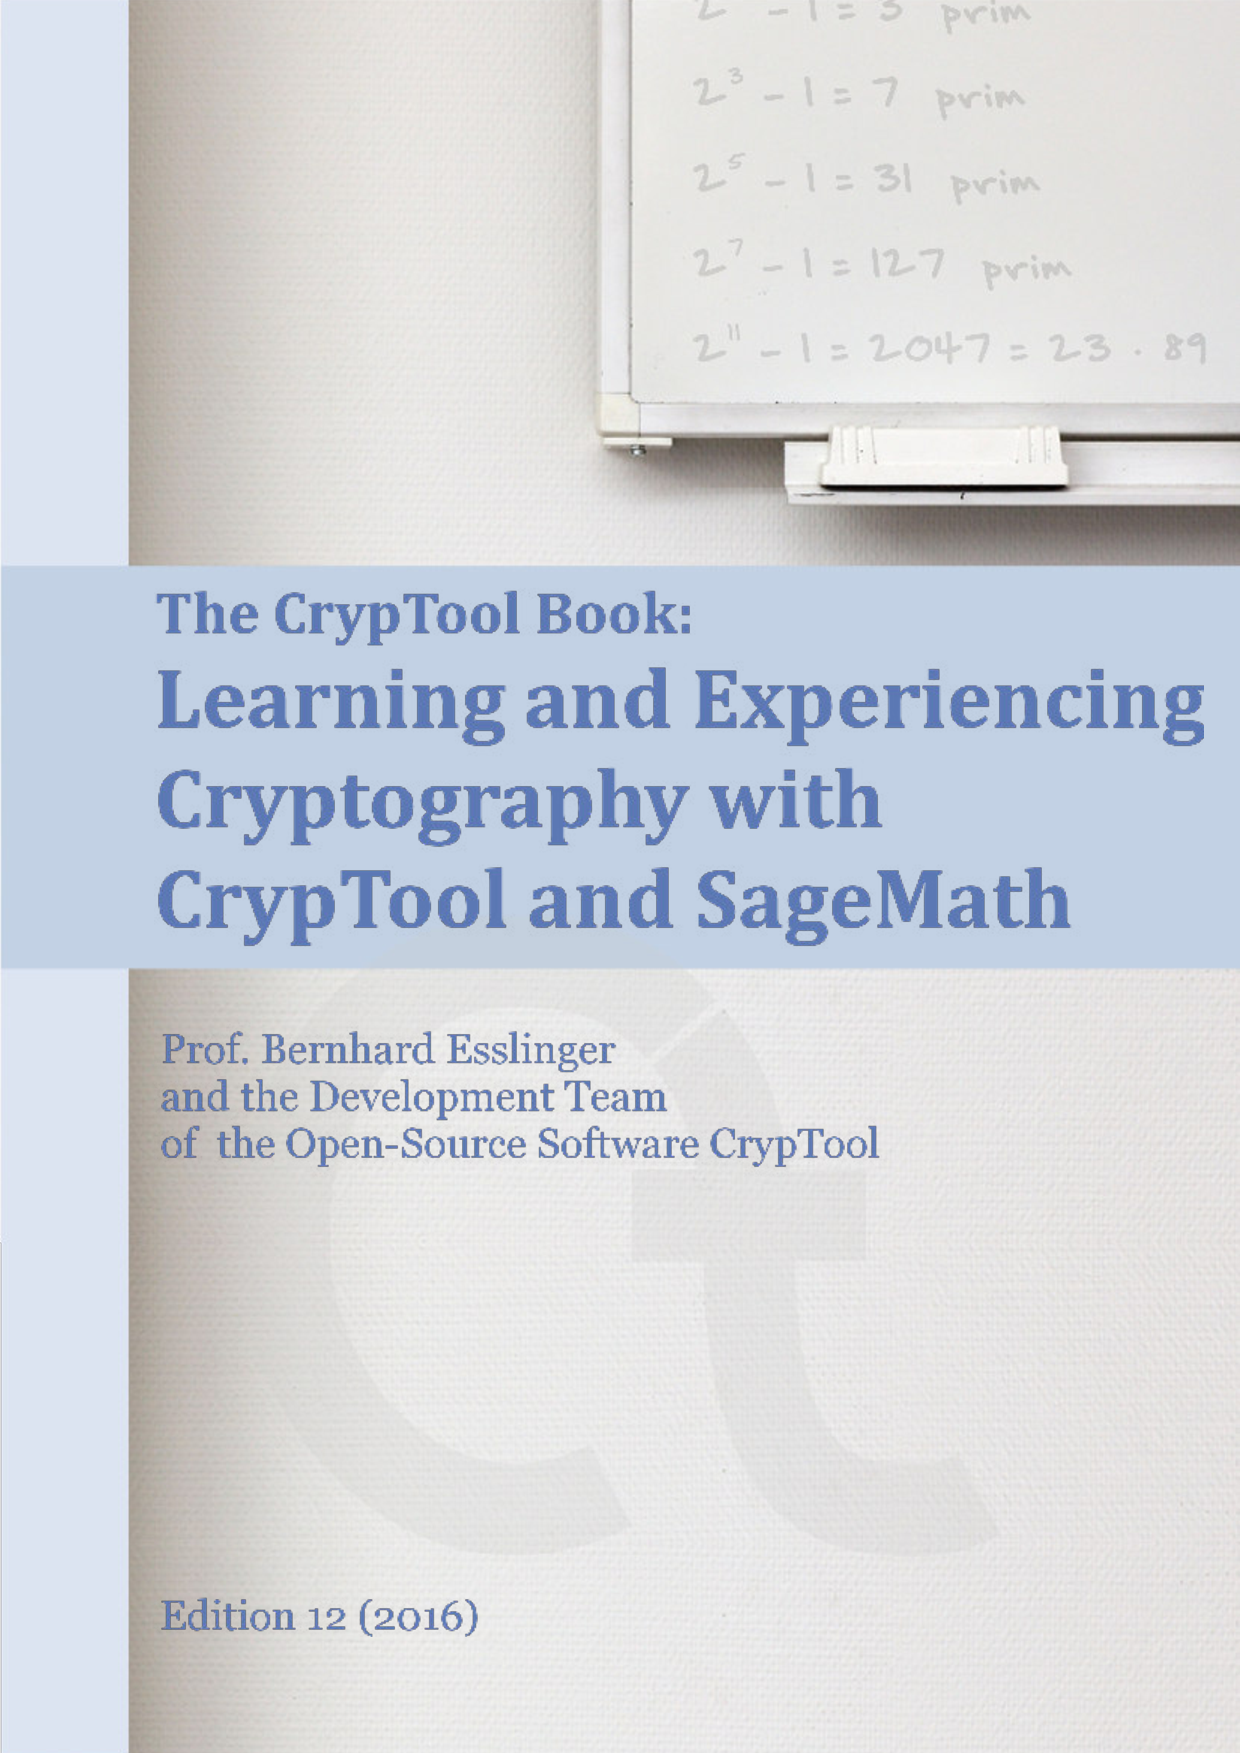
\includepdf[pages=1]{figures/coverv1_en_draft.pdf}   % 100dpi
% 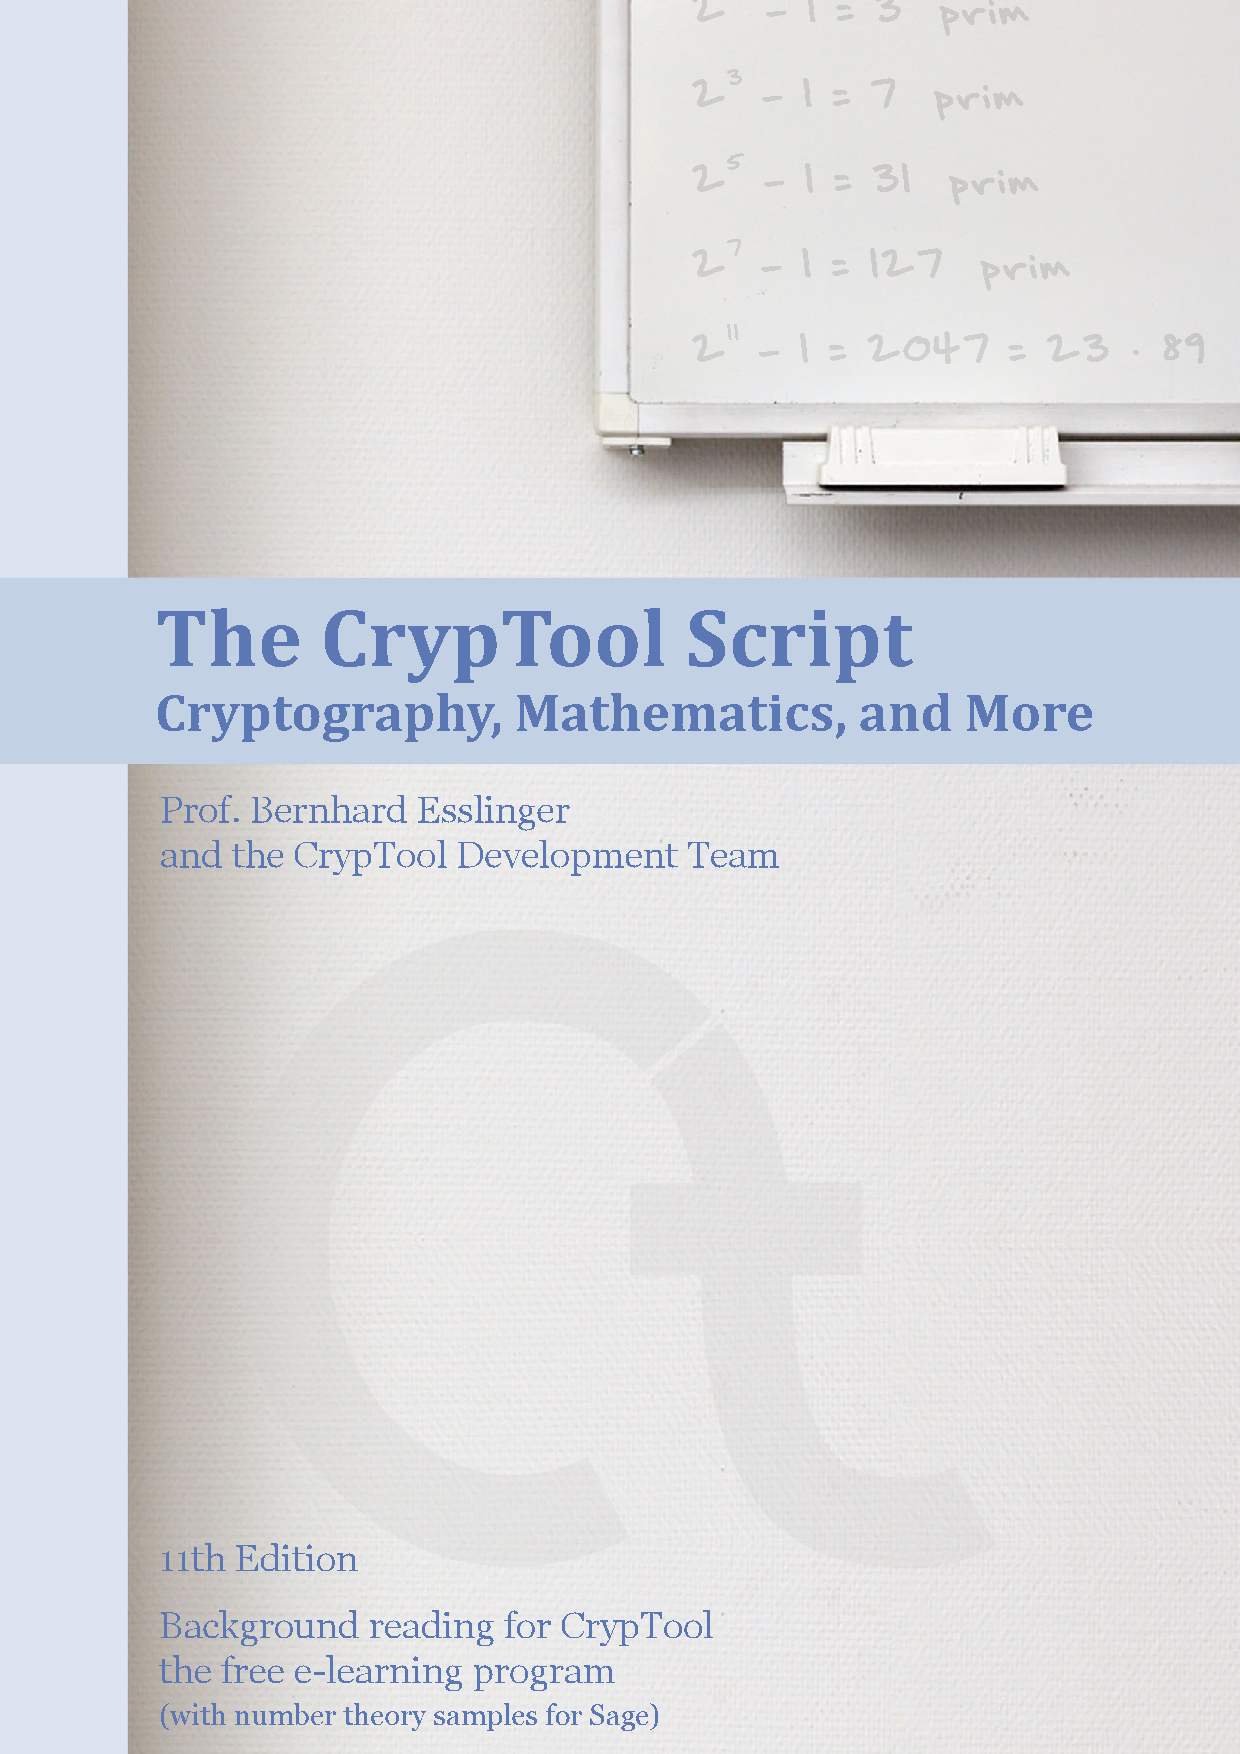
\includepdf[pages=1]{figures/coverv1_en.pdf}   % 300dpi

\pagestyle{plain}
\tikzset{ampersand replacement=\&} %DIF > %16xxxxxxxxxxxxxx

\setlength{\fboxrule}{.5mm}
\setlength{\fboxsep}{1.75mm}
\setlength{\footnotesep}{6pt}
\addtolength{\footskip}{8pt}

\VerbatimFootnotes
\renewcommand\footnoterule{%
  \vspace{2em}
  \hrule width .4\columnwidth
 \vspace{4pt}
}


\frontmatter
\maketitle


\begin{quote}
This is a free document, so the content of the document can
be copied and distributed, also for commercial purposes --- as long as
the authors, title and the CrypTool web site (\url{www.cryptool.org})
are acknowledged. Naturally, citations from the CrypTool book are
possible, as in all other documents.\\
Additionally, this document is liable to the specific license of the
GNU Free Documentation Licence.

    Copyright \copyright{} 1998--2017 Bernhard Esslinger and the
    CrypTool Team. Permission is granted to copy,
    distribute and/or modify this document under the terms of the GNU
    Free Documentation License, Version 1.3 or any later version
    published by the Free Software Foundation. A copy of
    the license is included in the section entitled
    \hyperlink{appendix-GNU-fdl}{``GNU Free Documentation License''}.

    This also includes the code of the SageMath samples in this document.
\end{quote}


\vspace{70pt}\noindent Suggestion for referencing with bibtex:
\begin{Verbatim}%
[fontsize=\footnotesize]
@book{Esslinger:ctb_2017,
  editor    = {Bernhard Esslinger},
  title     = {{L}earning and {E}xperiencing {C}ryptography
               with {C}ryp{T}ool and {S}age{M}ath},
  publisher = {CrypTool Project},
  edition   = {12},
  year      = {2017}
}
\end{Verbatim}


\vspace{250pt}
\noindent
Source cover photograph: \url{www.photocase.com}, Andre Guenther\\
Typesetting software: \LaTeX\\
Version control software: Subversion


% $Id: aboutcryptool.tex 3714 2016-04-08 18:34:16Z esslinger $
% !Mode:: "TeX:DE"    % Setting document mode and submode for WinEdt
% ............................................................................
%          Ü b e r b l i c k  (Text der 4. Seite, noch bevor Content)
%
% ~~~~~~~~~~~~~~~~~~~~~~~~~~~~~~~~~~~~~~~~~~~~~~~~~~~~~~~~~~~~~~~~~~~~~~~~~~~~

\clearpage
\setcounter{secnumdepth}{-1}  % Prevent this chapter title from having a number
\chapter%[Überblick]%
{Überblick über den Inhalt des CrypTool-Buchs}
\setcounter{secnumdepth}{4}  % Set back default from CT-Book-de.tex (show numbers till level 4)

Der Erfolg des Internets hat zu einer verstärkten
Forschung der damit verbundenen Technologien geführt, was auch im
Bereich Kryptographie viele neue Erkenntnisse schaffte.

In diesem {\em Buch zu den CrypTool-Programmen} \index{CrypTool} finden Sie
eher mathematisch orientierte Informationen zum Einsatz von
kryptographischen Verfahren. Zu einigen Verfahren gibt es Beispielcode,
geschrieben für das Computer-Algebra-System \textbf{SageMath}\index{SageMath}
(siehe Anhang~\ref{s:appendix-using-sage}).
Die Hauptkapitel sind von verschiedenen \textbf{Autoren} verfasst
(siehe Anhang~\ref{s:appendix-authors}) %\hyperlink{appendix-authors}{Autoren}
und in sich abgeschlossen. Am Ende der meisten Kapitel finden Sie
Literaturangaben und Web-Links.
Die Kapitel wurden reichlich mit {\em Fußnoten} versehen, in denen auch darauf
verwiesen wird, wie man die beschriebenen Funktionen in den verschiedenen
CrypTool-Programmen aufruft.

Das \hyperlink{Chapter_EncryptionSecDefinitions}{erste Kapitel} beschreibt
die Prinzipien der symmetrischen und asymmetrischen
\hyperlink{Chapter_EncryptionSecDefinitions}{\textbf{Verschlüsselung}} und
gibt Definitionen für deren Widerstandsfähigkeit.

Im \hyperlink{Chapter_PaperandPencil}{zweiten Kapitel} wird -- aus
didaktischen Gründen -- eine ausführliche Übersicht
über \hyperlink{Chapter_PaperandPencil}\textbf{Papier- und Bleistiftverfahren}
gegeben.

Ein großer Teil des Buchs ist dem faszinierenden Thema der
\hyperlink{Chapter_Primes}\textbf{Primzahlen} (Kapitel \ref{Chapter_Primes})
gewidmet.
Anhand vieler Beispiele wird in die \hyperlink{Chapter_ElementaryNT}\textbf{modulare Arithmetik}
und die \hyperlink{Chapter_ElementaryNT}\textbf{elementare Zahlentheorie}
(Kapitel \ref{Chapter_ElementaryNT}) eingeführt. Hier bilden die Eigenschaften
des \textbf{RSA-Verfahrens} einen Schwerpunkt.

Danach erhalten Sie Einblicke in die mathematischen Konzepte und
Ideen hinter der \hyperlink{Chapter_ModernCryptography}{\textbf{modernen Kryptographie}}
(Kapitel \ref{Chapter_ModernCryptography}).

%Ein \hyperlink{Chapter_Hashes-and-Digital-Signatures}{weiteres Kapitel}
Kapitel \ref{Chapter_Hashes-and-Digital-Signatures} gibt einen Überblick zum Stand der
Attacken gegen moderne \hyperlink{Chapter_Hashes-and-Digital-Signatures}\textbf{Hashalgorithmen}
und widmet sich dann kurz den \hyperlink{Chapter_Hashes-and-Digital-Signatures}\textbf{digitalen Signaturen}
--- sie sind unverzichtbarer Bestandteil von E-Business-Anwendungen.

Kapitel \ref{Chapter_EllipticCurves} stellt \hyperlink{Chapter_EllipticCurves}
\textbf{Elliptische Kurven} vor: Sie sind eine Alternative zu RSA und für die
Implementierung auf Chipkarten besonders gut geeignet.

Kapitel \ref{Chapter_BitCiphers} führt in die \hyperlink{Chapter_BitCiphers}\textbf{Boolesche Algebra} ein.
Boolesche Algebra ist Grundlage der meisten modernen, symmetrischen
Verschlüsselungsverfahren, da diese auf Bitströmen und Bitblöcken operieren.
Prinzipielle Konstruktionsmethoden dieser Verfahren werden beschrieben
und in SageMath implementiert.

Kapitel \ref{Chapter_HomomorphicCiphers} stellt
\hyperlink{Chapter_HomomorphicCiphers}\textbf{Homomorphe Kryptofunktionen}
vor: Sie sind ein modernes Forschungsgebiet, das insbesondere im Zuge des
Cloud-Computing an Bedeutung gewann.

Kapitel \ref{Chapter_Dlog-FactoringDead} beschreibt
\hyperlink{Chapter_Dlog-FactoringDead}\textbf{Aktuelle
Resultate zum Lösen diskreter Logarithmen und zur Faktorisierung}.
Es gibt einen breiten Überblick und Vergleich über die zur Zeit besten
Algorithmen für (a) das Berechnen diskreter Logarithmen in
verschiedenen Gruppen, für (b) das Faktorisierungsproblem und
für (c) Elliptische Kurven. Dieser Überblick wurde zusammengestellt,
nachdem ein provozierender Vortrag auf der Black Hat-Konferenz
2013 für Verunsicherung sorgte, weil er die Fortschritte bei endlichen
Körpern mit kleiner Charakteristik fälschlicherweise auf Körper
extrapolierte, die in der Realität verwendet werden.

Das \hyperlink{Chapter_Crypto2020}{letzte Kapitel}
\hyperlink{Chapter_Crypto2020}\textbf{Krypto 2020}
diskutiert Bedrohungen für bestehende kryptographische Verfahren und
stellt alternative Forschungsansätze (Post-Quantum-Kryptographie)
für eine langfristige kryptographische Sicherheit vor.

Während die CrypTool-\textit{eLearning-Programme}\index{eLearning} eher den
praktischen Umgang motivieren und vermitteln, dient das \textit{Buch} dazu,
dem an Kryptographie Interessierten ein tieferes Verständnis für die
implementierten mathematischen Algorithmen zu vermitteln -- und das
didaktisch mög"-lichst gut nachvollziehbar.

Die \hyperlink{appendix-start}\textbf{Anhänge}
\ref{s:appendix-menu-overview-CT1},
\ref{s:appendix-template-overview-CT2},
\ref{s:appendix-function-overview-JCT} und
\ref{s:appendix-function-overview-CTO}
erlauben einen schnellen Überblick über die Funktionen in den verschiedenen
CrypTool-Varianten\index{CT1}\index{CT2}\index{JCT}\index{CTO} via:
\begin{itemize}
  \item der Funktionsliste und
        dem \hyperlink{appendix-menu-overview-CT1}
                      {Menübaum von CrypTool~1 (CT1)},
  \item der Funktionsliste und
        den \hyperlink{appendix-template-overview-CT2}
                      {Vorlagen in CrypTool~2 (CT2)},
  \item der \hyperlink{appendix-function-overview-JCT}
                      {Funktionsliste von JCrypTool (JCT)}, und
  \item der \hyperlink{appendix-function-overview-CTO}
                      {Funktionsliste von CrypTool-Online (CTO)}.
\end{itemize}
%Anker sind \hypertarget{appendix-menutree}{} und \label{s:appendix-menutree}
%  - \hyperlink{}{} legt Link auf die Seite unter den Text in 2. Klammer
%  - \ref{} legt Link und fügt Kapitelnummer ein.

% Bernhard Esslinger, Matthias Büger, Bartol Filipovic, Henrik Koy, Roger Oyono
% und Jörg Cornelius Schneider
Die Autoren möchten sich an dieser Stelle bedanken bei den Kollegen
in der jeweiligen Firma und an den Universitäten Bochum, Darmstadt, Frankfurt,
Gießen, Karlsruhe, Lausanne, Paris und Siegen.

\enlargethispage{0.5cm}
Wie auch bei dem E-Learning-Programm CrypTool\index{CrypTool} wächst
die Qualität des Buchs mit den Anregungen und Verbesserungsvorschlägen
von Ihnen als Leser. Wir freuen uns über Ihre Rück"-mel"-dung.



% Local Variables:
% TeX-master: "../script-de.tex"
% End:



\newpage
\pdfbookmark[0]{Contents Overview}{ShortContents}
\shorttoc{Contents Overview}{0}
\clearpage\phantomsection
\pdfbookmark[0]{\contentsname}{Contents}
\tableofcontents 

\newpage
\normalsize

\newcounter{mycounterDefaultParskip}
\setcounter{mycounterDefaultParskip}{4}
\parskip \value{mycounterDefaultParskip} pt 


\renewcommand{\bibname}{Bibliography \CTBChapName{}}
\newcommand{\CTBChapName}{(Chap Intro)}           % $Id$
% ............................................................................
%      V O R W O R T  und  E I N F � H R U N G (Zusammenspiel Skript-CT) 
% ~~~~~~~~~~~~~~~~~~~~~~~~~~~~~~~~~~~~~~~~~~~~~~~~~~~~~~~~~~~~~~~~~~~~~~~~~~~~


% --------------------------------------------------------------------------
\section*{Preface to the 7th Edition of the CrypTool Script}
\addcontentsline{toc}{section}{Preface to the 7th Edition of the CrypTool Script}

Starting in the year 2000 this script became a part of the 
CrypTool\index{CrypTool} package. It is designed to accompany the program 
CrypTool by explaining some mathematical topics in more detail, 
but still in a way which is easy to understand.

In order to also enable developers/authors to work together independently 
the topics have been split up and for each topic an extra chapter has been 
written which can be read on its own. The later editorial work in TeX added 
cross linkages between different sections and footnotes describing where you
can find the according functions within the CrypTool\index{CrypTool} 
program \hyperlink{appendix-menutree}{(see menu tree in appendix A).}
% in \ref{s:appendix-menutree}   AUFPASSEN, DASS nichts doppelt !!
% \hypertarget{appendix-menutree}{}\label{s:appendix-menutree}
Naturally there are many more interesting topics in mathematics and
cryptography which could be discussed in greater depth -- therefore this
is only one of many ways to do it.

\vspace{12pt}
The rapid spread of the Internet has also lead to intensified research in the
technologies involved, especially within the area of cryptography where a good
deal of new knowledge has arisen.

This edition of the script adds some topics, but mainly updates areas (e.g. the
summaries of topical research areas):
\vspace{-7pt}
\begin{itemize}
  \item the search for the largest prime numbers (generalized Mersenne 
        and Fermat primes) \\ 
%        and Fermat primes, ``M-40'') 
	(chap. \ref{spezialzahlentypen}, \ref{zahlentyp_mersenne}), 
  \item the factorisation of big numbers (RSA-200)\index{RSA-200} 
        (chap. \ref{RSA-200}),
  \item progress in cryptanalysis of hash algorithms 
        (chap. \ref{collision-attacks-against-sha-1}),
  \item progress in ideas for new crypto methods (RSA successor) 
        (chap. \ref{xxxxxxxxxBrute-force-gegen-Symmetr})\index{xxxxxxxxxxxxxxxx} and
  \item a list, in which movies or novels cryptography or number theory has a 
        major role (see appendix \ref{s:appendix-movies}).
\end{itemize}

\vspace{12pt}
The first time the document was delivered with CrypTool\index{CrypTool} 
was in version 1.2.01. Since then it has been expanded and revised in almost every 
new version of CrypTool (1.2.02, 1.3.00, 1.3.02, 1.3.03, 1.3.04 and now 1.3.10).

I'd be more than happy if this also continues in the further open-source
versions of CrypTool\index{CrypTool}.

I am deeply grateful to all the people helping with their impressive
commitment who have made this global project so successful. Especially I would
like to acknowledge the English language proof-reading of this script version
done by Richard Christensen and Lowell Montgomery.

I hope that many readers have fun with this script and that they get 
out of it more interest and greater understanding of this modern but 
also very ancient topic.
\\


Bernhard Esslinger

Frankfurt (Germany), June 2005



% --------------------------------------------------------------------------
\newpage
\section*{Introduction -- How do the Script and the Program Play together?}  \addcontentsline{toc}{section}{Introduction -- How do the Script and the Program Play together?}


\textbf{This script}

This document is delivered together with the program CrypTool\index{CrypTool}.
\par \vskip + 3pt

The articles in this script are largely self-contained and
can also be read independently of CrypTool\index{CrypTool}.

Chapters  \ref{Chapter_ModernCryptography} (Modern Cryptography) and 
\ref{Chapter_EllipticCurves} (Elliptic Curves) require a deeper knowledge
in mathematics, while the other chapters should be understandable with a 
school leaving certificate.

The authors
% \hyperlink{appendix-authors}{(authors)}
% in \ref{s:appendix-authors}
% \hypertarget{appendix-authors}{}\label{s:appendix-authors}
have attempted to describe cryptography for a broad 
audience -- without being mathematically incorrect. We believe that this
didactical pretension is the best way to promote the awareness for IT
security and the readiness to use standardised modern cryptography.
\par \vskip + 15pt


\textbf{The program CrypTool\index{CrypTool}}

CrypTool\index{CrypTool} is a program with an extremely comprehensive online
help enabling you to use and analyse cryptographic procedures within a
unified graphical user interface.\par \vskip + 3pt

CrypTool\index{CrypTool} was developed during the end-user awareness program
at Deutsche Bank in order to increase employee awareness of IT security and provide them with
a deeper understanding of the term security.
A further aim has been to enable users to understand the cryptographic
procedures. In this way, using CrypTool
as a reliable reference implementation of the various encryption procedures
(because of using the industry-proven Secude library\index{SECUDE IT Security}),
you can test the encryption implemented in other programs. \par \vskip + 3pt

CrypTool\index{CrypTool} is currently been used for 
training in companies and teaching at school and universities, and
moreover several universities are helping to further develop the project.
\par \vskip + 15pt


\textbf{Acknowledgment}

At this point I'd like to thank explicitly six people who particularly 
contributed to CrypTool\index{CrypTool}. Without their special talents
 and engagement CrypTool would not be what it is today:
\vspace{-7pt}
\begin{itemize}
   \item Mr.\ Henrik Koy
   \item Mr.\ J\"org-Cornelius Schneider
   \item Dr.\ Peer Wichmann
   \item Prof. Dr. Claudia Eckert,  Mr.\ Thomas Buntrock and Mr.\ Thorsten Clausius.
\end{itemize}
Also I want to thank all the many people not mentioned here for their 
hard work (mostly carried out in their spare time).
\\

Bernhard Esslinger

Frankfurt (Germany), June 2005

% Local Variables:
% TeX-master: "../script-en.tex"
% End:

\mainmatter
\renewcommand{\CTBChapName}{(Chap CryptoMeth)}    % $Id$
% ............................................................................
%             V E R S C H L U E S S E L U N G S V E R F A H R E N
% ~~~~~~~~~~~~~~~~~~~~~~~~~~~~~~~~~~~~~~~~~~~~~~~~~~~~~~~~~~~~~~~~~~~~~~~~~~~~

\begin{bibunit}[babalpha] %% alpha: Chapter bibliography shows authors abbreviation


% HACK to fix warning "destination with the same identifier .. has already been used, ...":
% REMOVED, because it caused missing index entries
%\makeatletter \renewcommand{\thepage}{~\csname @arabic\endcsname \c@page} \makeatother

%%%% Old naming: \hypertarget{Kapitel_1}{}
\hypertarget{Chapter_EncryptionSecDefinitions}{}

\chapter{Sicherheits-Definitionen und Verschl�sselungsverfahren}
\label{Chapter_EncryptionSecDefinitions}
(\hyperlink{author_Bernhard-Esslinger}{Bernhard Esslinger},
 \hyperlink{author_Joerg-Cornelius-Schneider}{J�rg-Cornelius Schneider},
 Mai 1999; Updates: Dez. 2001, Feb. 2003, Juni 2005, Juli 2007, Jan. 2010, M�rz 2013, Aug. 2016)

Dieses Kapitel soll einen eher beschreibenden Einstieg bieten und die
Grundlagen ohne Verwendung von allzu viel Mathematik vermitteln.

Sinn der Verschl�sselung \index{Verschl�sselung} ist es, Daten so zu
ver�ndern, dass nur ein autorisierter Empf�n\-ger in der Lage ist,
den Klartext zu rekonstruieren. Das hat den Vorteil, dass verschl�sselte
Daten offen �bertragen werden k�nnen und trotzdem keine Gefahr besteht,
dass ein Angreifer die Daten unberechtigterweise lesen kann. Der
autorisierte Empf�nger ist im Besitz einer geheimen Information, des
sogenannten Schl�ssels, die es ihm erlaubt, die Daten zu entschl�sseln,
w�hrend sie jedem anderen verborgen bleiben.\footnote{%
  Nat�rlich kann ein Angreifer trotzdem die Verbindung st�ren oder
  Metadaten (wie wer mit wem kommuniziert) abgreifen.
}%\par \vskip + 3pt

Zur Erl�uterung verwenden wir im Folgenden die Begriffe aus der
Abbildung \ref{cm_Generic-Notations-when-Encrypting}:
\begin{figure}[ht]
\begin{center}
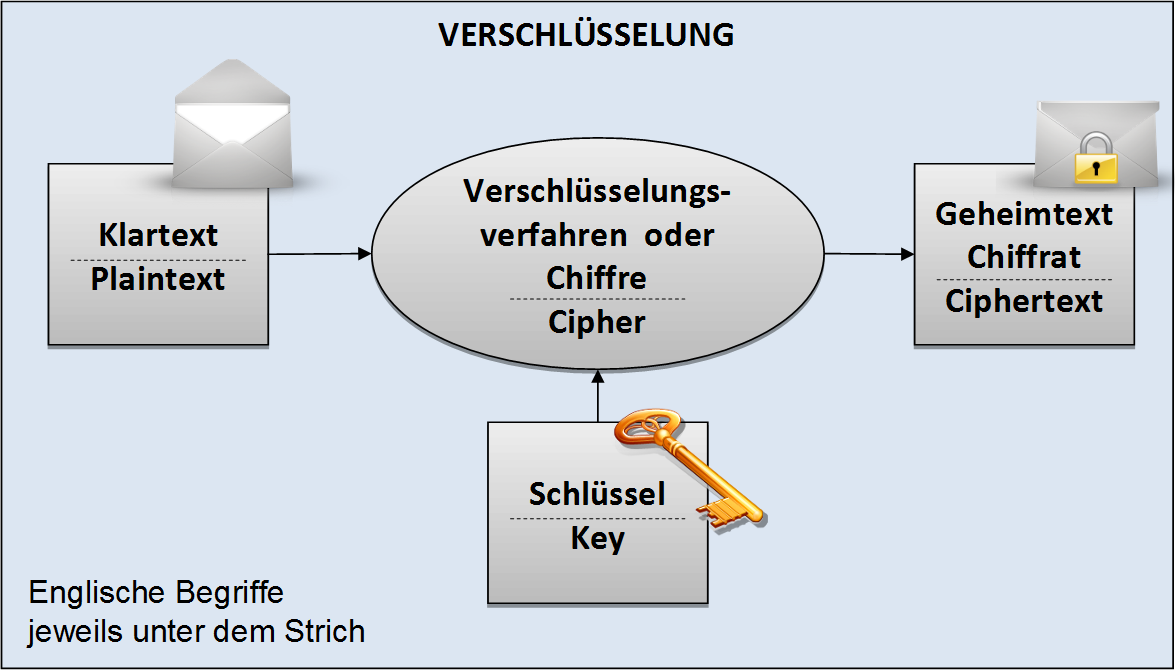
\includegraphics[scale=0.7]{figures/Generic-Notation-Encryption_de.png}
\caption{�bliche Bezeichnungen bei der Verwendung von Verschl�sselungsverfahren} 
\label{cm_Generic-Notations-when-Encrypting}
\end{center}
\end{figure}



% --------------------------------------------------------------------------
\newpage

\begin{ctsquote}
Erkl�re es mir, ich werde es vergessen.\\
Zeige es mir, ich werde es vielleicht behalten.\\
Lass es mich tun, und ich werde es k�nnen.
\caption{Indisches Sprichwort}
\end{ctsquote}


% --------------------------------------------------------------------------
\hypertarget{cm_Section_Security_Definitions}{}
\section{Sicherheits-Definitionen und Bedeutung der Kryptologie}
\label{cm_Section_Security_Definitions}
\index{Sicherheits-Definitionen}

Zuerst erkl�ren wir, wie die Sicherheit von Kryptosystemen definiert wird.

\noindent Moderne Kryptographie basiert vor allem auf mathematischer Theorie und
Computer-Praxis. Beim Design kryptographischer Algorithmen werden Annahmen
zur Schwierigkeit von Berechnungen so gemacht, so dass sich solche Verfahren
in der Praxis von einem Angreifer nur schwer brechen lassen.

\vskip +3pt
Die zwei Hauptnotationen in der Literatur definieren Sicherheit in
Abh�ngigkeit von den M�glichkeiten des Angreifers (vgl. z.B.
{\em Contemporary Cryptography} \cite{Oppliger2011}):

\begin{itemize}

\item {\bf Berechenbare, bedingte oder praktische Sicherheit}\\
  Ein Verschl�sselungsverfahren ist {\em berechenbar} sicher, wenn es (obwohl
  es theoretisch m�glich ist, es zu brechen) selbst mit den besten bekannten
  Verfahren nicht gebrochen werden kann. Theoretische Fortschritte (z.B.
  Verbesserungen bei den Algorithmen zur Faktorisierung) und schnellere
  Computer erfordern, dass dies st�ndig angepasst wird. 

  Selbst wenn man den besten bekannten Algorithmus zum Brechen benutzt, wird
  man so viele Ressourcen brauchen (z.B. 1.000.000 Jahre), dass das Kryptosystem
  sicher ist.

  Daher basiert dieses Konzept auf Annahmen �ber die begrenzte Rechenkraft des
  Angreifers und auf dem aktuellen Stand der Wissenschaft.

\item {\bf Informations-theoretische oder unbedingte Sicherheit}\\
  Ein Verschl�sselungsverfahren wird als {\em unbedingt} sicher bezeichnet,
  wenn seine Sicherheit gew�hrleistet ist, v�llig unabh�ngig davon, wieviele
  Ressourcen (Zeit, Speicher) der Angreifer hat -- also auch in dem Fall,
  wenn der Angreifer unbegrenzt viele Ressourcen hat, um das
  Verfahren zu brechen. Auch mit unbegrenzt vielen Ressourcen kann der
  Angreifer aus dem Chiffrat keine sinnvollen Informationen gewinnen.

  Es gibt Informations-theoretisch sichere Verfahren, die beweisbar nicht
  gebrochen werden k�nnen, auch nicht mit unendlich viel Rechenkraft -- ein
  Beispiel daf�r ist das {\em One-Time-Pad} (OTP\index{OTP}).

  Da das OTP ein Informations-theoretisch sicheres Verschl�sselungsverfahren
  ist, leitet sich seine Sicherheit schon allein aus der Informationstheorie
  ab -- und ist sicher, auch wenn der Angreifer unbegrenzte Rechenkapazit�ten
  hat. Das OTP weist allerdings einige praktische Nachteile auf (der
  verwendete Schl�ssel darf nur einmal verwendet werden, muss zuf�llig
  gew�hlt werden und mindestens so lang sein wie die zu sch�tzende Nachricht),
  so dass es au�er in geschlossenen Umgebungen, zum Beispiel beim hei�en
  Draht zwischen Moskau und Washington, kaum eine Rolle spielt.%\par \vskip + 3pt

\end{itemize}


\vskip +3pt
\noindent Manchmal werden auch zwei weitere Konzepte verwendet:

\begin{itemize}

\item {\bf Beweisbare Sicherheit}
Dies bedeutet, dass das Brechen eines Kryptosystems mindestens so schwierig ist
wie die L�sung eines bestimmten schwierigen Problems, z.B. die Berechnung des
diskreten Logarithmus, die diskrete Quadratwurzel-Berechnung oder die
Faktorisierung sehr gro�er Zahlen.

Beispiel: Aktuell wissen wir, dass RSA\index{RSA} h�chstens so schwierig
ist wie die Faktorisierung, aber wir k�nnen nicht beweisen, dass es genauso
schwierig ist.
Deshalb hat RSA keine beweisbare Mindest-Sicherheit. Oder in anderen Worten:
Wir k�nnen nicht beweisen, dass wenn das Kryptosystem RSA gebrochen ist, dass
dann auch die Faktorisierung (ein schwieriges mathematisches Problem) gel�st
werden kann.

Das Rabin-Kryptosystem war das erste Kryptosystem, f�r das sich beweisen lie�,
dass es berechenbar �quivalent zu einem harten mathematischen Problem ist.

\item {\bf Ad-hoc-Sicherheit}
Ein kryptographisches System hat diese Sicherheit, wenn es sich nicht lohnt,
es zu versuchen es zu brechen, weil der Aufwand daf�r teurer ist als der Wert
der Daten, die man durch das Brechen erhalten w�rde. Z.B. weil ein Angriff
nicht in einer ausreichend kurzen Zeit erfolgen kann (vgl.
{\em Handbook of Applied Cryptography} \cite{Menezes2001}).

Dies kann z.B. zutreffen, wenn B�rsen-relevante Daten sowieso am
n�chsten Tag ver�ffent"-licht werden und man f�r das Brechen ein Jahr brauchen
w�rde.

\end{itemize}


\vskip +3pt
Bei den heutzutage verwendeten guten Verfahren ist der Zeitaufwand zum Brechen
so hoch, dass sie praktisch nicht gebrochen werden k�nnen. Deshalb kann man
diese Verfahren als (praktisch) sicher ansehen -- aus einer rein auf den
Algorithmus bezogenen Sichtweise.\footnote{%
  Insbesondere seit den Informationen von Edward Snowden\index{Snowden, Edward} gab es
  viele Diskussionen, ob Verschl�sselung sicher ist. In \cite{Esslinger2014} wird das
  Ergebnis einer Evaluierung vorgestellt, auf welche Kryptographie man sich verlassen
  kann -- nach dem heutigen Kenntnisstand.
  Der Artikel untersucht: Welche Krypto-Verfahren k�nnen im Lichte der NSA-Enth�llungen
  noch als sicher gelten? Wo wurden Systeme gezielt geschw�cht? Wie k�nnen wir die
  kryptographische Zukunft sicher gestalten? Wie unterscheiden sich Mathematik und
  Implementierung?
}

\vskip +3pt
\begin{sloppypar}
Grunds�tz"-lich unterscheidet man zwischen symmetrischen
(siehe Kapitel \ref{cm_Section_Symmetric-encryption}) und asymmetrischen
(siehe Kapitel \ref{cm_Section_Asymmetric-encryption})
Verfahren zur Verschl�sse"-lung.
Einen sehr guten �berblick �ber die verschiedenen Verschl�sselungsverfahren
bieten auch die B�cher von Bruce Schneier \cite{Schneier1996} und Klaus Schmeh
\cite{Schm2016}.\footnote{%
  Einen kompakten �berblick, der erkl�rt, was wozu verwendet wird, welche der Verfahren
  sicher sind, wo mit Problemen zu rechnen ist und wo die wichtigen Baustellen f�r die
  absehbare Zukunft liegen incl. des Procederes bei den Standardisierungen finden Sie
  in \cite{Schmidt2016}.
  % TODO Info an ju, dass Schreibweise korr ("s" anh�ngen)
  %%     bei "Bereits 1883 formulierte Auguste Kerckhoff".
  % Dieser Artikel erschien urspr�nglich in c't 01/2016, Seite 174
  % Kryptographie in der IT - Empfehlungen zu Verschl�sselung und Verfahren.
  % Kryptographie ist ein wichtiger Baustein moderner IT � Sicherheit,
  % Vertraulichkeit und Privatsph�re h�ngen davon ab. Der folgende Krypto-Wegweiser
  % gibt einen kompakten �berblick zu den aktuell relevanten Verfahren.
}
\end{sloppypar}

\vskip +3pt
Bevor Verschl�sselungstechnologien mit dem Aufkommen des Internets und der drahtlosen
Kommunikation f�r jedermann zur Verf�gung standen, waren sie schon seit Jahrhunderten
im Gebrauch von Regierungen, Milit�rs und Diplomaten. Welche Seite diese Technologie
besser beherrschte konnte mit Hilfen der Geheimdienste gro�en Einfluss auf die {\bf Politik}
und den Kriegsverlauf nehmen. Auf die Historie geht dieses Buch nur insofern ein, als
in Kapitel \ref{Chapter_PaperandPencil} auch die fr�her benutzten Verfahren vorgestellt
werden. Einen Eindruck, welch entscheidende Bedeutung Kryptologie f�r die M�chtigen
hatte und hat, kann man anhand der beiden folgenden Beispiele bekommen: dem Lehrfilm
\glqq Krieg der Buchstaben\grqq\footnote{%
  Der Film \index{Krieg der Buchstaben} schildert vor dem Hintergrund der Weltpolitik
  von 1900-1945 die Entwicklung der Kryptologie und ihre Bedeutung f�r den
  Kriegsverlauf im ersten (Zimmermann-Depesche) und zweiten Weltkrieg. Ausf�hrlich
  wird -- aus anglo-amerikanischer Sicht -- darauf eingegangen, wie bedeutsam die
  Kryptoanalyse (auf dem Atlantik gegen die Enigma und auf dem Pazifik gegen Purple)
  f�r den Verlauf des zweiten Weltkriegs war.\\
  Siehe \url{http://bscw.schule.de/pub/bscw.cgi/d1269787/Krieg_der_Buchstaben.pdf}.
}
und der Debatte um die sogenannten Krypto-Wars\footnote{%
  Siehe \url{https://de.wikipedia.org/wiki/Crypto_Wars}.\index{Krypto-Wars}
}.
%% Vgl. http://scilogs.spektrum.de/hlf/verschluesselte-hintertuerchen-tag-internet-licht/
%%      http://www.heidelberg-laureate-forum.org/de/2015/08/17/eine-debatte-ueber-die-herausforderungen-einer-datengesteuerten-welt/
%%      http://wwwde.uni.lu/snt/news_events/prof_peter_ryan_gives_lecture_at_heidelberg_laureate_forum
%% Diskussion auf dem 3. Heidelberg Laureate Forum (HLF) am Dienstag, 25. August 2015.


% --------------------------------------------------------------------------
\newpage

\begin{ctsquote}
\glqq Man kann nicht nicht kommunizieren!\grqq 
\caption[Paul Watzlawick]{Paul Watzlawick\footnotemark}\index{Watzlawick, Paul}
\end{ctsquote}
\addtocounter{footnote}{0}\footnotetext{Paul Watzlawick, Janet H. Beavin und Don D. Jackson, \glqq Menschliche Kommunikation. Formen, St�rungen, Paradoxien\grqq, Huber, (c) 2007, Das erste der f�nf pragmatischen Axiome ihrer Kommunikationstheorie.}

% --------------------------------------------------------------------------
\section[Einfl�sse auf Verschl�sselungsverfahren] % Was zw. [..] steht, kommt ins Inhaltsverzeichnis!
{Einfl�sse auf Verschl�sselungsverfahren}

% \nopagebreak
Hier sollen kurz zwei Aspekte von Kryptoverfahren erw�hnt werden, auf die oft nicht fr�h genug eingegangen wird:

\begin{itemize}

\item {\bf Zufallsbasiert}\\
\index{Zufall}
Man kann Algorithmen aufteilen in deterministische\index{deterministisch} und heuristische\index{heuristisch} Verfahren. Meistens lernten Studenten nur deterministische Verfahren kennen, bei denen die Ausgabe eindeutig durch die Eingabe vorgegeben wird. Bei heuristischen Verfahren werden Entscheidungen aufgrund zuf�lliger Werte getroffen. Moderne Verfahren des maschinellen Lernens geh�ren ebenfalls hierzu.

In Kryptoverfahren spielt Zufall eine gro�e Rolle. Immer m�ssen die Schl�ssel zuf�llig gew�hlt werden, so dass zumindest bei der Schl�sselgenerierung~\glqq Zufall\grqq~erzeugt werden muss. Zus�tzlich sind manche Verfahren (vor allem aus der Kryptoanalyse) heuristisch.

\item {\bf Konstanten-basiert}\\
Viele moderne Verfahren (insbesondere Hashverfahren und symmetrische Verschl�sse-lungsverfahren) benutzen numerische Konstanten. Diese sollten nachvollziehbar sein und keine Hintert�ren erm�glichen. Zahlen, die das erf�llen, nennt man im Englischen~\glqq Nichts-im-�rmel\grqq-Zahlen: Nothing-up-my-sleeve number\index{Zahlen!Nothing-up-my-sleeve}.%
\footnote{\url{http://en.wikipedia.org/wiki/Nothing_up_my_sleeve_number}}

\end{itemize}


\newpage
Die folgende Abbildung \ref{cm_Figure_OTP-demo-pictures} soll eine Idee davon vermitteln, dass es nicht m�glich ist, bei einem OTP\index{OTP} den Klartext zu bestimmen (sofern das OTP-Verfahren richtig angewendet wird und alle Schl�ssel gleich wahrscheinlich sind).

In dem Beispiel in der Abbildung ist als Geheimtext ein 8 Zeichen langes Wort gegeben:
\texttt{11 1B 1E 18 00 04 0A 15}.
Es gibt viele sinnvolle Worte aus 8 Buchstaben und zu jedem einen passenden Schl�ssel.
Ein Angreifer kann damit allein nicht bestimmen, welches der richtige Schl�ssel bzw.
welches das richtige Klartext-Wort ist.

Vergleiche auch Abbildung~\ref{fig-bool-otp} in Kapitel \ref{s-bool-bitstr-real-random},
wo ein entsprechendes Text-Beispiel mit SageMath erstellt wird.
\begin{figure}[ht]
\begin{center}
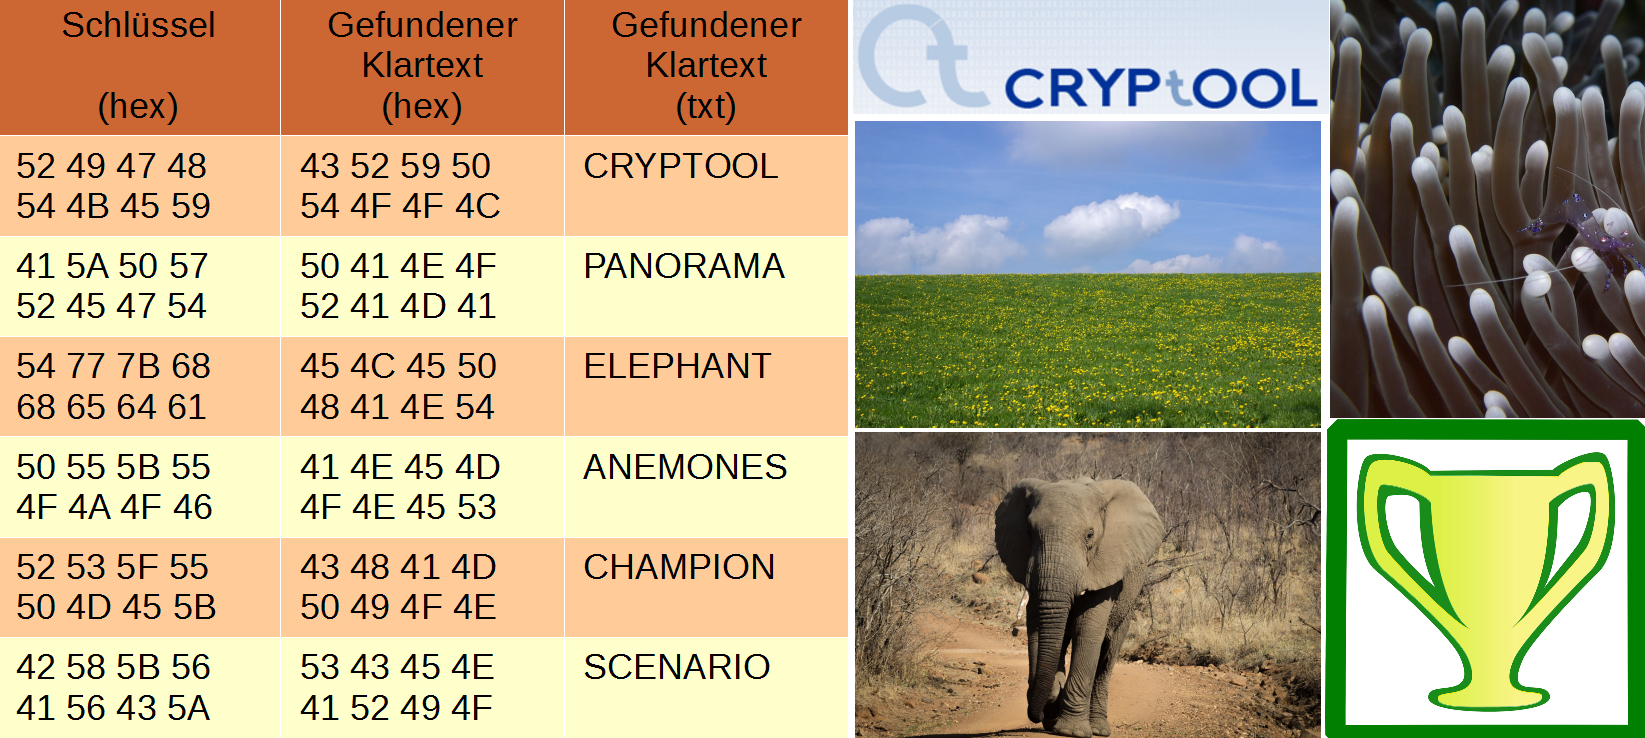
\includegraphics[scale=0.55]{figures/OTP-demo-pictures-de.png}
\caption[Illustration f�r die Informations-theoretische Sicherheit des OTP]
        {Illustration f�r die Informations-theoretische Sicherheit des OTP\footnotemark}
\label{cm_Figure_OTP-demo-pictures}
\end{center}
\end{figure}
\footnotetext{
  Bildquelle: Kostenlose Bilder von \url{https://pixabay.com/}
}





% --------------------------------------------------------------------------
\newpage

\begin{ctsquote}
\glqq Transparenz. Das ist das H�chste, was man sich in einer technologisch hoch entwickelten Gesellschaft erhoffen kann ... sonst wird man einfach nur manipuliert.\grqq 
\caption[Daniel Suarez]{Daniel Suarez\footnotemark}\index{Suarez, Daniel}
\end{ctsquote}
\addtocounter{footnote}{0}\footnotetext{Daniel Suarez, \glqq Darknet\grqq,
            rororo, (c) 2011, Kapitel 5, \glqq Einsichten\grqq, S. 69, Price.}

% --------------------------------------------------------------------------
\section[Symmetrische Verschl�sselung] % Was zwischen [...] steht, kommt ins Inhaltsverzeichnis!
        {Symmetrische Verschl�sselung\footnotemark}
  \footnotetext{% Dieses Prozent ist n�tig, sonst startet die Fu�note mit einem Blank !
    Mit CrypTool~1 ({\bf CT1})\index{CT1} k�nnen Sie �ber das
    Men� {\bf Ver-/Entschl�sseln \textbackslash{} Symmetrisch (modern)} folgende
    modernen symmetrischen Verschl�sselungsverfahren ausf�hren:\\
    IDEA, RC2, RC4, DES (ECB), DES (CBC), Triple-DES (ECB), Triple-DES (CBC),
    MARS (AES-Kandidat), RC6 (AES-Kandidat), Serpent (AES-Kandidat), 
    Twofish (AES-Kandidat),
    Rijndael (offizielles AES-Verfahren)\index{AES}.\\
    Mit CrypTool~2 ({\bf CT2})\index{CT2} k�nnen Sie im Startcenter
    �ber {\bf Vorlagen \textbackslash{} Kryptographie \textbackslash{}
    Modern \textbackslash{} Symmetrisch} folgende modernen symmetrischen
    Verschl�sselungsverfahren ausf�hren:\\ 
    AES, DES, PRESENT, RC2, RC4, SDES, TEA, Triple-DES, Twofish.\\
    In JCrypTool ({\bf JCT})\index{JCT} stehen Ihnen die folgenden
    modernen symmetrischen Verschl�sselungsverfahren zur Verf�gung:\\ 
    AES, Rijndael, Camellia, DES, Dragon, IDEA, LFSR, MARS, Misty1, RC2, RC5,
    RC6, SAFER+, SAFER++, Serpent, Shacal, Shacal2, Twofish.
    }
\label{cm_Section_Symmetric-encryption}

\nopagebreak

Bei der {\em symmetrischen} Verschl�sselung 
\index{Verschl�sselung!symmetrisch} m�ssen Sender und Empf�nger
�ber einen gemeinsamen (geheimen) Schl�ssel verf�gen, den sie vor
Beginn der eigentlichen Kommunikation ausgetauscht haben. Der Sender
benutzt diesen Schl�ssel, um die Nachricht zu verschl�sseln und der
Empf�nger, um diese zu entschl�sseln.\par %\vskip + 3pt

Dies veranschaulicht Abbildung \ref{cm_Figure_Symmetric-Enc_Secret-Key-Enc}:
\begin{figure}[ht]
\begin{center}
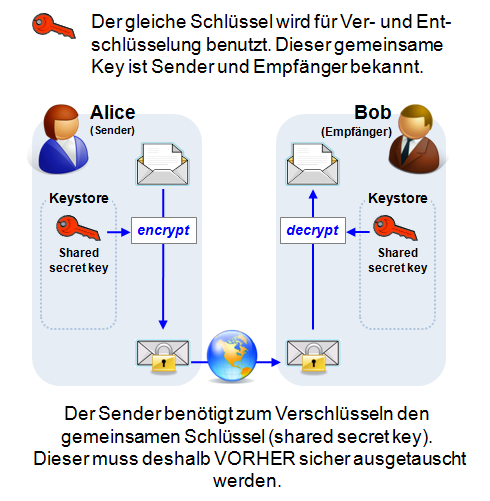
\includegraphics[scale=0.7]{figures/SymmetricEnc_Figure_Chap1_de.png}
\caption{Symmetrische oder Secret-Key-Verschl�sselung} 
\label{cm_Figure_Symmetric-Enc_Secret-Key-Enc}
\end{center}
\end{figure}

Alle klassischen Chiffren sind vom Typ symmetrisch. Beispiele dazu finden Sie
in den CT-Programmen, im Kapitel~\ref{Chapter_PaperandPencil}
(\glqq \nameref{Chapter_PaperandPencil}\grqq)
in diesem Skript oder in \cite{Nichols1996}. 
In diesem Unterkapitel wollen wir jedoch nur die moderneren symmetrischen
Verfahren betrachten.

Vorteile von symmetrischen Algorithmen sind die hohe
Geschwindigkeit, mit denen Daten ver- und entschl�sselt werden.
Ein Nachteil ist das Schl�sselmanagement. Um miteinander
vertraulich kommunizieren zu k�nnen, m�ssen Sender und
Empf�nger vor Beginn der eigentlichen Kommunikation �ber einen
sicheren Kanal einen Schl�ssel ausgetauscht haben. Spontane
Kommunikation zwischen Personen, die sich vorher noch nie begegnet
sind, scheint so nahezu unm�glich. Soll in einem Netz mit $ n $
Teilnehmern jeder mit jedem zu jeder Zeit spontan kommunizieren
k�nnen, so muss jeder Teilnehmer vorher mit jedem anderen der
$n - 1$ Teilnehmer einen Schl�ssel ausgetauscht haben. Insgesamt
m�ssen also $n(n - 1)/2$ Schl�ssel ausgetauscht werden.\par \vskip + 3pt



\subsection[AES (Advanced Encryption Standard)]{AES (Advanced Encryption Standard)\footnotemark} 
\footnotetext{%
   In CT1\index{CT1} finden Sie 3 Visualisierungen dieses Verfahrens
   �ber das Men� {\bf Einzelverfahren \textbackslash{} Visualisierung von
   Algorithmen \textbackslash{} AES}.\\
   In CT2\index{CT2} k�nnen Sie im Startcenter
   mit dem Suchstring \glqq AES\grqq~eine Vorlage (Template) finden,
   die den Algorithmus Schritt-f�r-Schritt visualisiert.
}
\label{CM_AES}
\index{AES}

Vor AES war der DES-Algorithmus\index{DES} das bekannteste moderne, symmetrische
Verschl�sselungs"-ver"-fahren. Der DES-Algorithmus war eine Entwicklung von IBM 
in Zusammenarbeit mit der National Security Agency \index{NSA} (NSA). 
Er wurde 1975 als Standard ver�ffentlicht. Trotz seines relativ hohen
Alters ist bis heute kein~\glqq effektiver\grqq~Angriff auf
ihn gefunden worden. Der effektivste Angriff besteht aus dem Durchprobieren
(fast) aller m�glichen Schl�ssel, bis der richtige gefunden wird 
({\em Brute-Force-Angriff})\index{Angriff!Brute-Force}. Aufgrund der relativ
kurzen Schl�ssell�nge von effektiv 56 Bits (64 Bits, die allerdings 8
Parit�tsbits enthalten), sind in der Vergangenheit schon mehrfach mit dem
DES verschl�sselte Nachrichten gebrochen worden, so dass er heute nicht
mehr als sicher anzusehen ist. Alternativen zum DES sind zum Beispiel die
Algorithmen IDEA\index{IDEA}, Triple-DES (TDES) und vor allem AES.
\par \vskip + 3pt

Standard unter den symmetrischen Verfahren ist heute AES\index{AES}:
Der dazu geh�rende Rijndael-Algo"-rithmus wurde am 2. Oktober 2000 zum
Gewinner der AES-Ausschreibung erkl�rt und ist damit Nachfolger
des DES-Verfahrens.

Einen Einstieg und weitere Verweise zum AES-Algorithmus und den AES-Kandidaten
der letzten Runde finden Sie z.B. in der Online-Hilfe von
CrypTool\index{CrypTool}%
\footnote{%
      Online-Hilfe von CT1\index{CT1}: Das Stichwort {\bf AES} im Index
      f�hrt auf die drei Hilfeseiten: {\bf AES-Kandidaten}, 
      {\bf Der AES-Gewinner Rijndael} und {\bf Der AES-Algorithmus Rijndael}.\\
      Eine ausf�hrliche Beschreibung von AES mit C-Code findet sich
      in \cite{Haan2008}.
  }
oder in Wikipedia%
\footnote{%
	\url{https://de.wikipedia.org/wiki/Advanced_Encryption_Standard}
  }.


\clearpage
\noindent Die beiden Screenshots \ref{AES-Visualization-Zabala-Flash-step3} und
\ref{AES-Visualization-Zabala-Flash-step5} sind aus einer der 3
AES-Visualisierungen in CT1\index{CT1}.

% Ohne das !vor ht verteilt LaTeX die abb. auf 2 Seiten. \sloppypar hilft hier nict (nur f�r Worttrenner).
% http://texwelt.de/wissen/fragen/6667/mehrere-bilder-untereinander
\begin{figure}[!ht]
\begin{center}
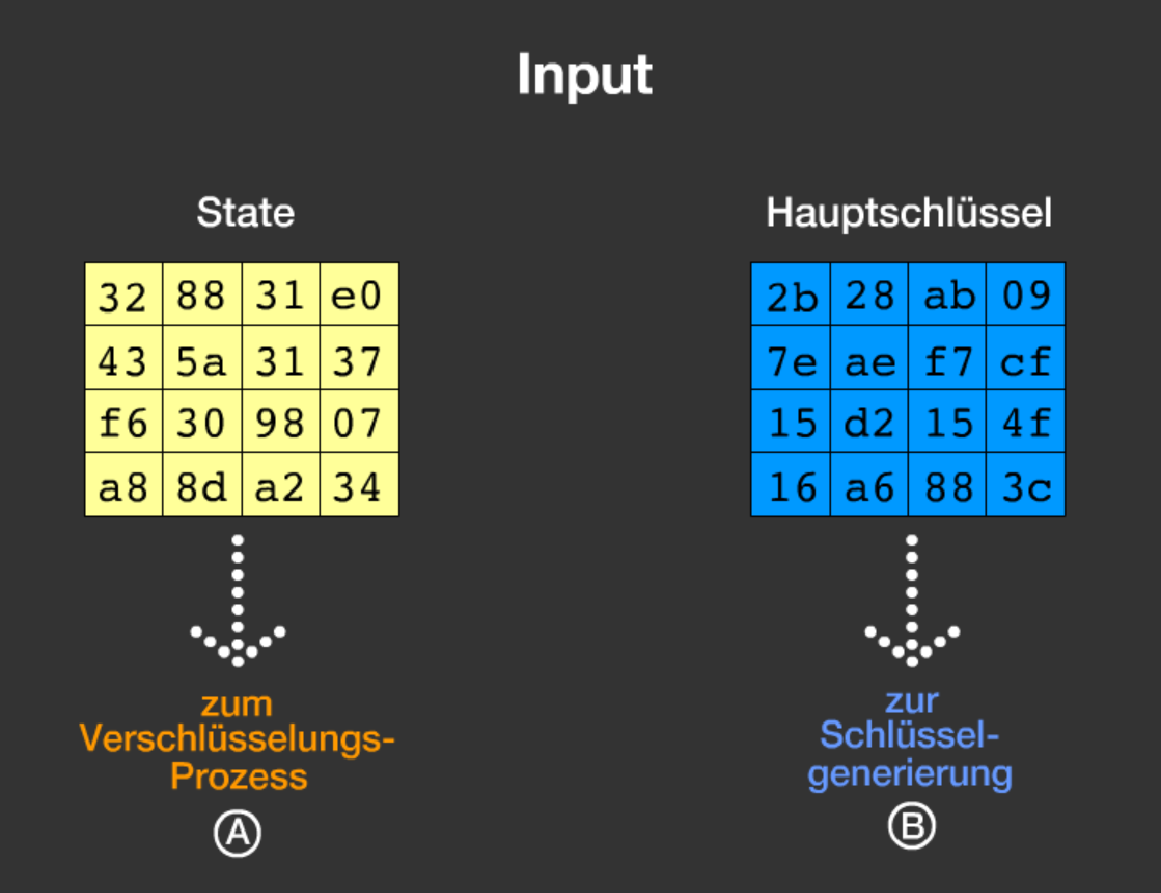
\includegraphics[scale=0.6]{figures/AES-Visualization-Zabala-Flash-step3_de}
\caption{AES-Visualisierung von Enrique Zabala aus CT1 (Teil 1)}
\label{AES-Visualization-Zabala-Flash-step3}
\end{center}
\end{figure}

\begin{figure}[!ht]
\begin{center}
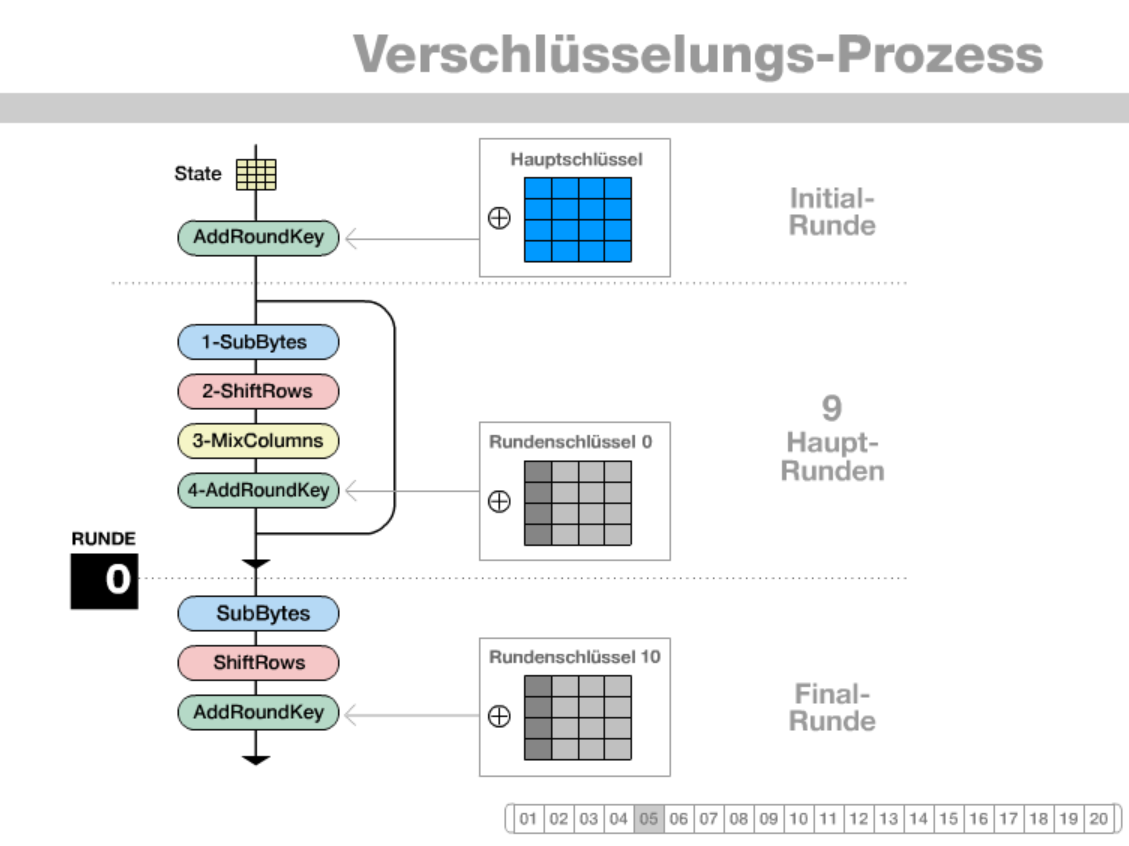
\includegraphics[scale=0.6]{figures/AES-Visualization-Zabala-Flash-step5_de}
\caption{AES-Visualisierung von Enrique Zabala aus CT1 (Teil 2)}
\label{AES-Visualization-Zabala-Flash-step5}
\end{center}
\end{figure}
%\end{sloppypar}


\clearpage
\noindent Im Folgenden wollen wir einen 128-bit-Block Klartext mit einem 128-bit
Schl�ssel mit AES im CBC-Modus verschl�sseln. Vom erhaltenen Geheimtext interessiert
uns nur der 1. Block (wenn mehr vorhanden ist, ist das Padding -- hier Null-Padding).
Zur Veranschaulichung machen wir das einmal mit CT2 und einmal mit OpenSSL.\\

\noindent Abbildung \ref{AES_Encrypting-one-block-with-CT2} zeigt die Verschl�sselung
eines Blocks in {\bf CT2}\index{CT2}.

\noindent Der Klartext \glqq AESTEST1USINGCT2\grqq~wird nach Hex
(41 45 53 54 45 53 54 31 55 53 49 4E 47 43 54 32)
konvertiert. Damit und mit dem Schl�ssel 3243F6A8885A308D313198A2E0370734
erzeugt die AES-Komponente dann den Geheimtext. Dieser lautet in Hex:\\
B1 13 D6 47 DB 75 C6 D8 47 FD 8B 92 9A 29 DE 08

\begin{figure}[ht]
\begin{center}
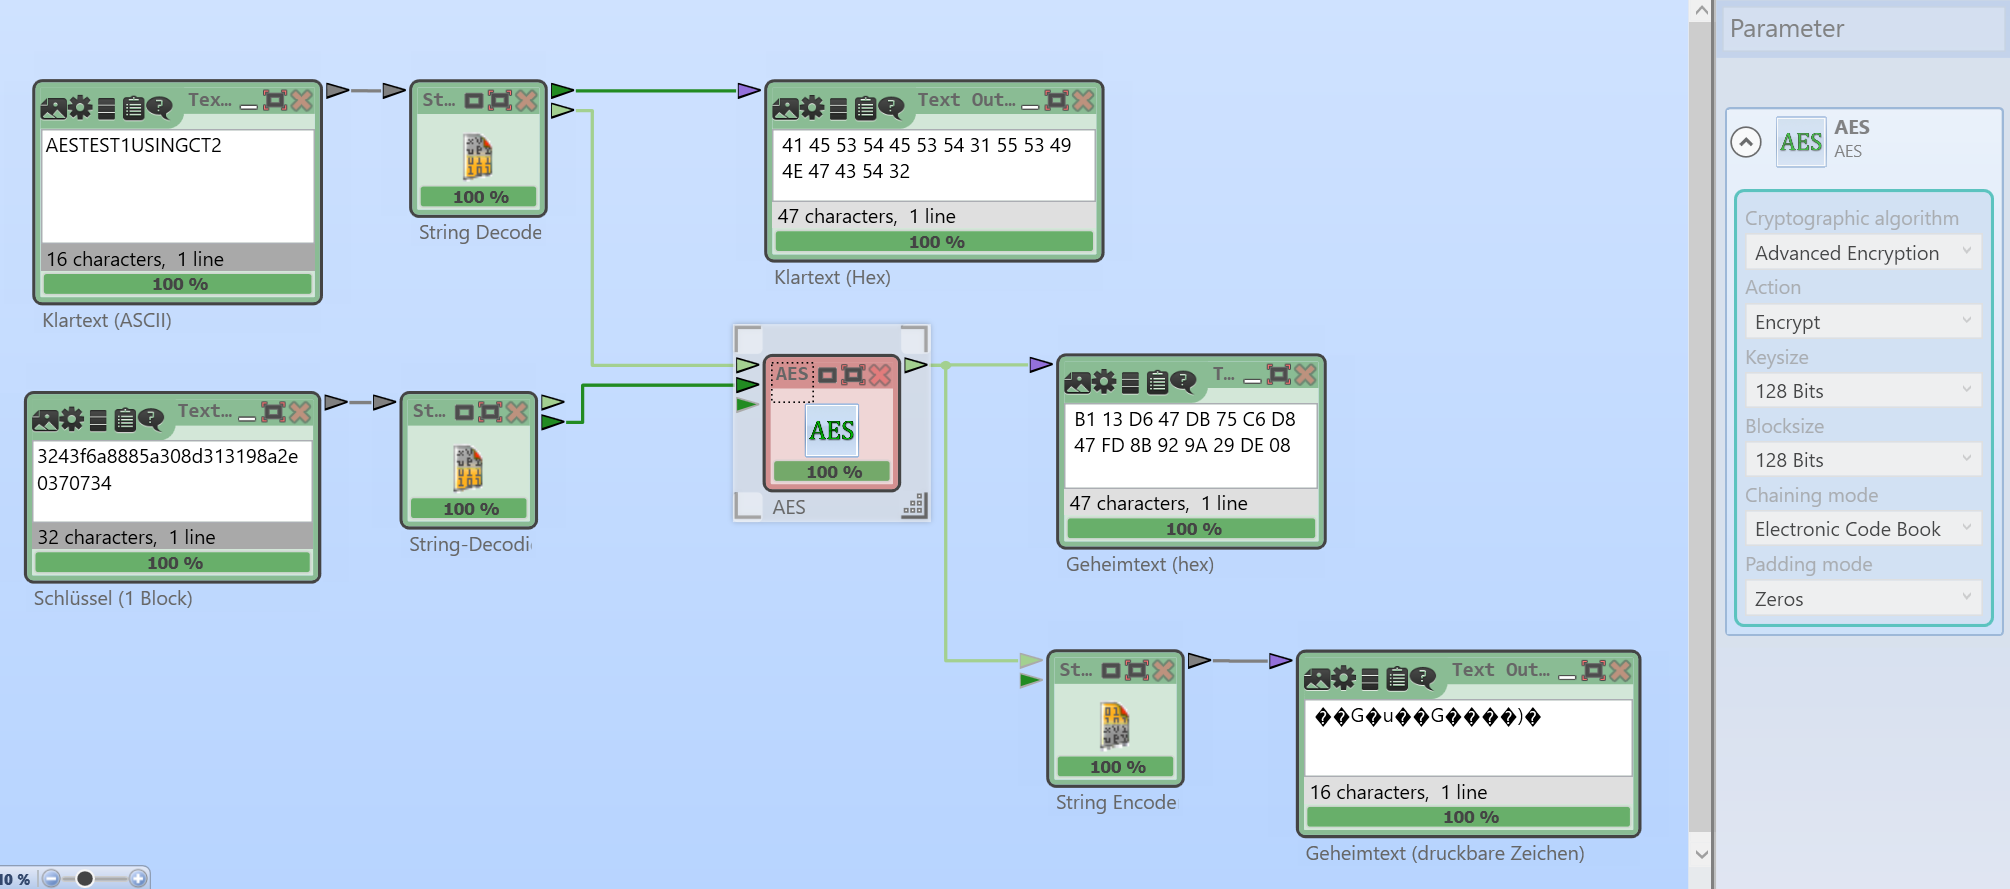
\includegraphics[scale=0.42]{figures/AES_Encrypting-one-block-with-CT2_de}
\caption{AES-Verschl�sselung (genau 1 Block ohne Padding) in CT2} 
\label{AES_Encrypting-one-block-with-CT2}
\end{center}
\end{figure}

\vspace{15pt}
\noindent Dasselbe Ergebnis kann man mit {\bf OpenSSL}\index{OpenSSL}%
\footnote{%
      OpenSSL\index{OpenSSL} ist eine sehr verbreitete freie Open-Source Kryptobibliothek,
      die von vielen Anwendungen benutzt wird, bspw. um das TLS-Protokoll zu implementieren.
      Zu OpenSSL geh�rt auch das Kommandozeilentool openssl, mit dem man die Funktionalit�t
      auf vielen Betriebssystemen direkt ausprobieren und Zertifikate beantragen, erzeugen
      und verwalten kann.\\
      Im Gegensatz zum ebenfalls sehr verbreiteten und sehr guten Kommandozeilentool gpg
      von GNU Privacy Guard\index{GnuPG}
      (\url{https://de.wikipedia.org/wiki/GNU_Privacy_Guard})
      erlaubt openssl auch Aufrufe, die sehr ins Detail gehen.
      Bei gpg liegt der Schwerpunkt auf den im praktischen Einsatz befindlichen Ciphersuites.
      Einfach genau einen Block ohne Padding zu verschl�sseln geht unseres Wissens mit dem
      Kommandozeilentool gpg nicht.\\
      Siehe auch \url{https://de.wikipedia.org/wiki/OpenSSL}.
%      Also see \url{https://en.wikipedia.org/wiki/OpenSSL}.
  }
auf der Kommandozeile auf ff. Weise erzielen:
\begin{opensslcode}
\begin{Verbatim}%
[fontsize=\footnotesize]
>openssl enc -e -aes-128-cbc
        -K 3243F6A8885A308D313198A2E0370734
        -iv 00000000000000000000000000000000
        -in klartext-1.hex  -out klartext-1.hex.enc
>dir
06.07.2016  12:43                16 key.hex
20.07.2016  20:19                16 klartext-1.hex
20.07.2016  20:37                32 klartext-1.hex.enc
\end{Verbatim}
\caption{AES-Verschl�sselung (von genau einem Block ohne Padding) in OpenSSL}
\label{cm_AES_no-padding:OpenSSL_example}
\end{opensslcode}





\clearpage
% HACK to fix warning "destination with the same identifier .. has already been used, ...":
% REMOVED, because it caused missing index entries
%\makeatletter \renewcommand{\thepage}{\csname @arabic\endcsname \c@page} \makeatother
% --------------------------------------------------------------------------
\subsubsection{Ergebnisse zur theoretischen Kryptoanalyse von AES}
\label{cm_New-AES-Analysis}
\index{Kryptoanalyse}
\index{AES}

Im Anschluss finden Sie einige Informationen, die das AES-Verfahren in
letzter Zeit in Zweifel zogen -- unserer Ansicht nach aber (noch)
unbegr�ndet. Die folgenden Informationen beruhen vor allem auf den unten
angegebenen Originalarbeiten und auf \cite{Wobst2002} und
\cite{Lucks2002}.

Der AES bietet mit einer Mindestschl�ssell�nge von 128 Bit gegen
Brute-Force-Angriffe auch auf l�ngere Sicht gen�gend Sicherheit -- es sei
denn, es st�nden entsprechend leistungsf�hige Quantencomputer zur
Verf�gung. Der AES war immun gegen alle bis dahin bekannten
Krypto"-analyse-Verfahren, die vor allem auf statistischen
�berlegungen beruhen und auf DES angewandt wurden: man konstruiert aus
Geheim- und Klartextpaaren Ausdr�cke, die sich nicht rein zuf�llig
verhalten, sondern R�ckschl�sse auf den verwendeten Schl�ssel zulassen.
Dazu waren aber unrealistische Mengen an abgeh�rten Daten n�tig.

Bei Kryptoverfahren bezeichnet man solche Kryptoanalyseverfahren als
"`akademischen Erfolg"' oder als "`kryptoanalytischen Angriff"', da sie
theoretisch schneller sind als das Durchprobieren aller Schl�ssel, das
beim Brute-Force-Angriff\index{Angriff!Brute-Force} verwendet wird. Im
Fall des AES mit maximaler Schl�ssell�nge (256 Bit) braucht die
ersch�pfende Schl�sselsuche im Durchschnitt $2^{255}$
Verschl�sselungsoperationen. Ein kryptoanalytischer Angriff muss diesen
Wert unterbieten. Als aktuell gerade noch praktikabel (z.B. f�r einen
Geheimdienst) gilt ein Aufwand von $2^{75}$ bis $2^{90}$
Verschl�sselungsoperationen.

Eine neue Vorgehensweise wurde in der Arbeit von Ferguson, Schroeppel
und Whiting im Jahre 2001 \cite{Ferguson2001} beschrieben: Sie stellten
AES als geschlossene Formel (in der Form einer Art Kettenbruch) dar,
was aufgrund seiner "`relativ"' �bersichtlichen Struktur gelang. Da
diese Formel aus rund 1 Billiarde Summanden besteht, taugt sie zun�chst
nicht f�r die Kryptoanalyse. Dennoch war die wissenschaftliche Neugier
geweckt. Bereits bekannt war, dass sich der 128-Bit-AES als ein
�berbestimmtes System von rund 8000 quadratischen Gleichungen
(�ber algebraischen Zahlk�rpern) mit rund 1600 Variablen (einige
Unbekannte sind die Schl�sselbits) darstellen l�sst -- solch gro�e
Gleichungssysteme sind praktisch nicht l�sbar. Dieses Gleichungssystem
ist relativ d�nn besetzt (\glqq sparse\grqq), d.h. von den insgesamt etwa
1.280.000 m�glichen quadratischen Termen tauchen nur relativ wenige
�berhaupt im Gleichungssystem auf.

Die Mathematiker Courtois und Pieprzyk \cite{Courtois2002} ver�ffentlichten 
2002 eine Arbeit, die in der Krypto-Szene stark diskutiert wird: Sie 
entwickelten das auf der Eurocrypt 2000 von Shamir et al. vorgestellte 
XL-Verfahren (eXtended Linearization) weiter zum XSL-Verfahren 
(eXtended Sparse Linearization). Das XL-Verfahren ist eine heuristische 
Technik, mit der es manchmal gelingt, gro�e nicht-lineare Gleichungssysteme 
zu l�sen und die bei der Analyse eines asymmetrischen Algorithmus (HFE) 
angewandt wurde.  Die Innovation von Courtois und Pieprzyk war, das 
XL-Verfahren auf symmetrische Verfahren anzuwenden: Das XSL-Verfahren kann
auf spezielle Gleichungssysteme angewandt werden. Damit k�nnte ein 
256-Bit-AES-Verfah"-ren in rund $2^{230}$ Schritten geknackt werden. Dies ist 
zwar immer noch ein rein akademischer Angriff, aber er ist richtungsweisend
f�r eine ganze Klasse von Blockchiffren. Das generelle Problem mit diesem
Angriff besteht darin, dass man bisher nicht angeben kann, unter welchen
Umst�nden er zum Erfolg f�hrt: die Autoren geben in ihrer Arbeit notwendige
Bedingungen an; es ist nicht bekannt, welche Bedingungen hinreichend sind.
Neu an diesem Angriff war erstens, dass dieser Angriff nicht auf Statistik,
sondern auf Algebra beruhte. Dadurch erscheinen Angriffe m�glich, die nur
geringe Mengen von Geheimtext brauchen. Zweitens steigt damit die Sicherheit
eines Produktalgorithmus%
\index{Produktalgorithmus}\index{Verschl�sselung!Produktalgorithmus}%
\footnote{%
Ein Geheimtext kann selbst wieder Eingabe f�r eine Chiffrierung sein. Eine
Mehrfachverschl�sselung (cascade cipher)
\index{Verschl�sselung!Mehrfachverschl�sselung}\index{Mehrfachverschl�sselung}
\index{Kaskaden}
entsteht aus einer Komposition von mehreren Verschl�sselungstransformationen.
Die Gesamtchiffrierung wird Produktalgorithmus oder Kaskadenalgorithmus
genannt (manchmal ist die Namensgebung abh�ngig davon, ob die verwendeten
Schl�ssel statistisch abh�ngig oder unabh�ngig sind).\\
Nicht immer wird die Sicherheit eines Verfahrens durch Produktbildung 
erh�ht.\\
Dieses Vorgehen wird auch {\em innerhalb} moderner Algorithmen angewandt:
Sie kombinieren in der Regel einfache und, f�r sich genommen, kryptologisch
relativ unsichere Einzelschritte in mehreren Runden zu einem leistungsf�higen
Gesamtverfahren. Die meisten modernen Blockchiffrierungen (z.B. DES, IDEA)
sind Produktalgorithmen.\\
Als Mehrfachverschl�sselung wird auch das Hintereinanderschalten desselben
Verfahrens mit verschiedenen Schl�sseln wie bei Triple-DES bezeichnet.\index{DES!Triple-DES}
}
nicht mehr exponentiell mit der Rundenzahl.

Aktuell wird sehr intensiv auf diesem Gebiet geforscht: z.B. stellten
Murphy und Robshaw auf der Crypto 2002 ein Papier vor \cite{Robshaw2002a},
das die Kryptoanalyse drastisch verbessern k�nnte: Der Aufwand f�r
128-Bit-Schl�ssel wurde auf $2^{100}$ gesch�tzt, indem sie AES als
Spezialfall eines Algorithmus BES (Big Encryption System) darstellten,
der eine besonders "`runde"' Struktur hat. Aber auch $2^{100}$
Rechenschritte liegen jenseits dessen, was praktisch in absehbarer Zeit
realisierbar ist. Bei 256 Bit Schl�ssell�nge sch�tzen die Autoren
den Aufwand f�r den XSL-Angriff auf $2^{200}$ Operationen.

Weitere Details finden Sie unter den Weblinks bei
\hyperlink{CM_HT_Weblink_Rijndael-Cryptosystem}{\glqq Das AES-/Rijndael-Kryptosystem\grqq}.
% nur \href oder \url r�ckt nicht ein, deshalb \item dazu !
%\vspace{-10pt}
%\begin{itemize}
%  \item[] \url{http://www.cryptosystem.net/aes} \\
%          \url{http://www.minrank.org/aes/} 
%\end{itemize}


F�r AES-256 w�re der Angriff ebenfalls viel besser als
Brute-Force\index{Angriff!Brute-Force}, aber noch weit au�erhalb der
Reichweite realisierbarer Rechenpower.

\begin{sloppypar}
Die Diskussion ist z.Zt. sehr kontrovers: Don Coppersmith (einer der
DES-Erfinder) z.B. bezweifelt die generelle Durchf�hrbarkeit des Angriffs:
XLS liefere f�r AES gar keine L�sung \cite{Coppersmith2002}. Dann w�rde
auch die Optimierung von Murphy und Robshaw \cite{Robshaw2002b} nicht
greifen.
\end{sloppypar}

2009 ver�ffentlichten Biryukov und Khovratovich \cite{Biryukov2009} einen
weiteren theoretischen Angriff auf AES, der sich anderer Techniken bedient, als
die oben vorgestellten. Sie verwenden Methoden aus der Kryptoanalyse von
Hashfunktionen (lokale Kollisionen und das Boomerang-Verfahren) und
konstruierten daraus einen Related-Key-Angriff auf AES-256. D.~h.\ der Angreifer
muss nicht nur in der Lage sein, beliebige Daten zu verschl�sseln (chosen plain
text), sondern auch den ihm unbekannten Schl�ssel manipulieren k�nnen (related
key).

Unter diesen Angriffs-Voraussetzungen reduziert der Angriff den Aufwand, einen
AES-256-Schl�ssel zu ermitteln, auf eine (asymmetrische) Komplexit�t von
$2^{119}$ Zeit und $2^{77}$ Speicher. Bei AES-192 ist der Angriff noch weniger
praktikabel, f�r AES-128 geben die Autoren keinen Angriff an.


% --------------------------------------------------------------------------
\subsection{Algebraische oder algorithmische Kryptoanalyse symmetrischer Verfahren}
\index{Angriff!algebraisch}
\label{cm_Algebraic-versus-Symmetr}

Es gibt unterschiedliche moderne Angriffsverfahren, die die Strukturen eines Problems direkt oder nach einer Transformation des Problems angreifen. Eines dieser Angriffsverfahren beruht auf dem Erf�llbarkeitsproblem der Aussagenlogik (SAT, von englisch satisfiability)%
\footnote{%
 \url{http://de.wikipedia.org/wiki/Erf%C3%BCllbarkeitsproblem_der_Aussagenlogik}
}.


%\vskip +25 pt
\paragraph*{Beschreibung SAT-Solver}\index{SAT-Solver}\mbox{}
\hypertarget{ht_SAT-Solver}{}

Ein sehr altes und gut studiertes Problem in der Informatik ist das sogenannte SAT-Problem. Hier gilt es, f�r eine gegebene Boolesche Formel herauszufinden, ob es eine Belegung der Variablen gibt, so dass die Auswertung der Formel den Wert 1 ergibt. 

Beispiel: Die Formel \glqq A UND B\grqq~wird zu 1 ausgewertet, wenn A=B=1 gilt. F�r die Formel \glqq A UND NICHT(A)\grqq~gibt es keine Belegung f�r A, so dass sie zu 1 ausgewertet wird.

F�r gr��ere Formeln ist es nicht so einfach herauszufinden, ob eine Formel zu 1 ausgewertet werden kann (dieses Problem geh�rt zu den NP-vollst�ndigen Problemen). Daher wurden spezielle Tools entwickelt, um dieses Problem f�r generelle Boolesche Formeln zu l�sen, sogenannte SAT-Solver\footnote{
    Mit {\bf CT2}\index{CT2} k�nnen Sie im Startcenter
    �ber {\bf Vorlagen \textbackslash{} Mathematisch \textbackslash{}
    SAT-Solver (Texteingabe)}  und  {\bf SAT-Solver (Dateieingabe)} einen
    SAT-Solver aufrufen.
    }. Wie sich herausgestellt hat, k�nnen SAT-Solver auch eingesetzt werden, um Krypto-Verfahren
anzugreifen.


%\vskip +25 pt
\paragraph*{SAT-Solver basierte Kryptoanalyse}\index{SAT-Solver}\mbox{}
\hypertarget{ht_SAT-Solver_Cryptanalysis}{}

Der generelle Ansatz, um SAT-Solver in der Kryptoanalyse einzusetzen, ist sehr einfach: Zun�chst wird das kryptographische Problem, etwa das Finden des symmetrischen Schl�ssels oder die Umkehrung einer Hashfunktion, in ein SAT-Problem �bersetzt. Dann wird ein SAT-Solver verwendet, um eine L�sung f�r das SAT-Problem zu finden. Die L�sung des SAT-Problems l�st dann auch das urspr�ngliche kryptographische Problem.
Der Artikel von Massacci \cite{Massacci2000} beschreibt die erste bekannte Verwendung eines SAT-Solvers in diesem Kontext. Leider stellte sich sehr bald heraus, dass ein solch genereller Ansatz in der Praxis nicht effizient eingesetzt werden kann. Die kryptographischen SAT-Probleme sind sehr komplex und die Laufzeit eines SAT-Solvers w�chst exponentiell mit der Problemgr��e. Daher werden in modernen Ans�tzen SAT-Solver nur f�r das L�sen von Teilproblemen der Kryptoanalyse verwendet. Ein gutes Beispiel zeigt der Artikel von Mironov und Zhang \cite{Mironov2006}. Hier wird anhand eines Angriffs auf Hashfunktionen gezeigt, zur L�sung welcher Teilprobleme SAT-Solver effizient eingesetzt werden k�nnen.

% Todo later: xxxxxxxxx Bsp aus CT2.1 erg�nzen mit SAT-Analyzer (nicht nur SAT-Solver)
%             Erfordert wahrscheinlich den CT2-Store, da es vorerst nur mit cygwin l�uft.
% \index{ZZZ6b-xxxxxxxxxxxxxxxx-Bsp aus CT2.1 ergaenzen} 
% \index{ZZZ6b-xxxxxxxxxxxxxxxxD}




% --------------------------------------------------------------------------
\subsection{Aktueller Stand der Brute-Force-Angriffe auf symmetrische Verfahren}
\index{Angriff!Brute-Force}
\index{RC5}
\label{cm_Brute-force-versus-Symmetr}

Anhand der Blockchiffre RC5 kann der aktuelle Stand von Brute-Force-Angriffen
auf symmetrische Verschl�sselungsverfahren gut erl�utert werden.

\begin{sloppypar}
Als Brute-Force-Angriff (exhaustive search, trial-and-error) bezeichnet
man das vollst�ndige Durchsuchen des Schl�sselraums: Dazu m�ssen
keine besonderen Analysetechniken eingesetzt werden. Stattdessen wird
der Geheimtext mit allen m�glichen Schl�sseln des Schl�sselraums
entschl�sselt%
\footnote{%
  Mit CT1\index{CT1} k�nnen Sie �ber das Men�
  {\bf Analyse \textbackslash{} Symmetrische Verschl�sselung (modern)}
  ebenfalls Brute-Force-Analysen von modernen symmetrischen Verfahren
  durchf�hren (unter der schw�chsten aller m�glichen Annahmen: Der
  Angreifer kennt nur den Geheimtext, er f�hrt also einen
  Ciphertext-only-Angriff durch).\\
  Mit CT2\index{CT2} k�nnen Sie bei den Vorlagen unter
  {\bf Kryptoanalyse \textbackslash{} Modern} ebenfalls Brute-Force-Analysen
  durchf�hren. Besonders m�chtig ist die KeySearcher-Komponente, die
  die Ausf�hrung auch auf mehrere Rechner verteilen kann.
}
und gepr�ft, ob der resultierende Text einen sinnvollen
Klartext ergibt%
\footnote{%
  Ist der Klartext nat�rlich-sprachlich und wenigstens 100 B lang, kann
  diese Pr�fung ebenfalls automatisiert durchgef�hrt werden.\\
  Um in einer sinnvollen Zeit auf einem Einzel-PC ein Ergebnis zu
  erhalten, sollten Sie nicht mehr als 24 Bit des Schl�ssels als
  unbekannt kennzeichnen.}.
Bei einer Schl�ssell�nge von 64 Bit sind dies maximal
$2^{64}$ = 18.446.744.073.709.551.616 oder rund 18 Trillionen zu
�berpr�fende Schl�ssel\index{CrypTool}.
\end{sloppypar}

Um zu zeigen, welche Sicherheit bekannte symmetrische Verfahren wie
DES, Triple-DES oder RC5\index{DES}\index{RC5}\index{DES!Triple-DES}
haben, veranstaltete z.B. RSA Security
sogenannte Cipher-Challenges\index{Challenge}.\footnote{%
  \url{https://www.emc.com/emc-plus/rsa-labs/historical/the-rsa-laboratories-secret-key-challenge.htm}\\
  Im Mai 2007 meldete RSA Inc leider, dass sie die Korrektheit der bis dahin
  nicht gel�sten RC5-72 Challenge nicht best�tigen werden.

  Cipher-Challenges gibt es auch f�r asymmetrische Verfahren
  (siehe Kapitel \ref{nt:NoteFactorization}).

  Ein weites Spektrum einfacher und komplexer, symmetrischer und asymmetrischer
  R�tsel-Aufgaben bietet der internationale Krypto-Wettbewerb
  {\bf MysteryTwister C3}: %% \glqq MysteryTwister C3\grqq:
  \url{http://www.mysterytwisterc3.org}.
  \index{MTC3}\index{Krypto-Wettbewerb}
  }
Unter kontrollierten Bedingungen wurden Preise ausgelobt, um Geheimtexte
(verschl�sselt mit verschiedenen Verfahren und verschiedenen
Schl�ssell�ngen) zu entschl�sseln und den symmetrischen Schl�ssel
zu ermitteln. Damit werden theoretische Resultate praktisch best�tigt.

Dass das "`alte"' Standard-Verfahren DES mit der fixen Schl�ssell�nge
von 56 Bit nicht mehr sicher ist, wurde schon im Januar 1999 von der
Electronic Frontier Foundation (EFF) demonstriert, als sie mit Deep Crack
eine DES-verschl�sselte Nachricht in weniger als einem Tag
knackten.\footnote{%
  \url{https://www.emc.com/emc-plus/rsa-labs/historical/des-challenge-iii.htm}
}

Der aktuelle Rekord f�r starke symmetrische Verfahren liegt bei 64 Bit
langen Schl�sseln. Dazu wurde das Verfahren RC5 benutzt, eine
Blockchiffre mit variabler Schl�ssell�nge. 

Die RC5-64 Challenge wurde im Juli 2002 nach 5 Jahren vom
distributed.net-Team gel�st.\footnote{%
 \url{http://www.distributed.net/Pressroom_press-rc5-64}\\
 \url{http://www.distributed.net/images/9/92/20020925_-_PR_-_64_bit_solved.pdf}
}
Insgesamt arbeiteten 331.252 Personen gemeinsam �ber das Internet
zusammen.\footnote{%
Eine �bersicht �ber die aktuellen Projekte zum verteilten Rechnen finden
Sie unter:\\
\url{http://distributedcomputing.info/}
}
Ge"-testet wurden rund 15 Trillionen Schl�ssel, bis der
richtige Schl�ssel gefunden wurde.%
\footnote{%
  CT2\index{CT2} hat begonnen, mit einer allgemeinen Infrastruktur f�r verteiltes
  Rechnen zu experimentieren (CrypCloud\index{CrypCloud}, die sowohl Peer-to-Peer
  als zentralisiert eingesetzt werden kann). Damit wird CT2 in der Zukunft in die
  Lage versetzt, Berechnungen auf viele Computer zu verteilen.
  Was man erreichen kann, wenn die Komponenten f�r die Parallelisierung eingerichtet
  sind, zeigte ein Cluster zur verteilten Kryptoanalyse von DES und AES:
  Stand 21. M�rz 2016 funktionierte ein Brute-force-Angriff (verteilte Schl�sselsuche)
  gegen AES auf 50 i5-PCs, jeder mit 4 virtuelles CPU-Kernen. Diese 200 virtuellen
  \glqq Worker Threads\grqq~konnten ca. 350 Millionen AES-Schl�ssel/sec testen. Die
  \glqq Cloud\grqq~verarbeitete dabei insgesamt ca. 20 GB/sec an Daten. CrypCloud
  ist eine Peer-to-Peer-basierte Cloud, so dass CT2-Nutzer sich freiwillig bei
  verteilten Jobs anschlie�en k�nnen.
}


Somit sind symmetrische Verfahren (auch wenn sie keinerlei
kryptographische Schw�"-chen haben) mit 64 Bit langen Schl�sseln
keine geeigneten Verfahren mehr sind, um sensible Daten l�nger geheim
zu halten.




% --------------------------------------------------------------------------
\newpage
\section[Asymmetrische Verschl�sselung] % Was zw. [..] steht, kommt ins Inhaltsverzeichnis!
{Asymmetrische Verschl�sselung\footnotemark}
  \footnotetext{%
   Das RSA-Kryptosystem kann mit CT1\index{CT1} �ber das Men� 
   {\bf Einzelverfahren \textbackslash{} RSA-Kryptosystem \textbackslash{} 
   RSA-Demo} in vielen Variationen nachvollzogen werden.\\
   Mit CT1\index{CT1} k�nnen Sie �ber das Men�
   {\bf Ver-/Entschl�sseln \textbackslash{} Asymmetrisch} mit RSA 
   ver- und entschl�sseln. In beiden F�llen m�ssen Sie ein 
   RSA-Schl�sselpaar ausw�hlen. Nur bei der Entschl�sselung wird der 
   geheime RSA-Schl�ssel ben�tigt -- deshalb wird nur hier die PIN abgefragt.\\
   Mit CT2\index{CT2} k�nnen Sie bei den Vorlagen unter
   {\bf Kryptographie \textbackslash{} Modern} ebenfalls asymmetrische
   Verfahren durchf�hren.\\
   JCT\index{JCT} bietet asymmetrische Verfahren wie RSA sowohl im
   Men� {\bf Visualisierungen} der Standard-Perspektive als auch in der
   Algorithmen-Perspektive.%Funktionalen
  }
\label{cm_Section_Asymmetric-encryption}

Bei der {\em asymmetrischen} Verschl�sselung
\index{Verschl�sselung!asymmetrisch} hat jeder Teilnehmer 
ein pers�nliches Schl�sselpaar, % Schl�s\-selpaar, be_24.5.03: so vorher und kam auch richtig raus! 
das aus einem {\em geheimen} \index{Schl�ssel!geheim} und einem 
{\em �ffentlichen} Schl�ssel \index{Schl�ssel!�ffentlich} besteht.
Der �ffentliche Schl�ssel wird, der Name deutet es an,
�ffentlich bekanntgemacht -- zum Beispiel in einem Schl�sselverzeichnis
im Internet (diese Art von \glqq Schwarzem Brett\grqq~wird auch Directory oder
�ffentlicher Schl�sselring genannt) oder in einem sogenannten \index{Zertifikat} Zertifikat.
\par \vskip + 3pt

Die asymmetrische Verschl�sselung veranschaulicht Abbildung \ref{cm_Figure_Asymmetric-Enc_Public-Key-Enc}:
\begin{figure}[ht]
\begin{center}
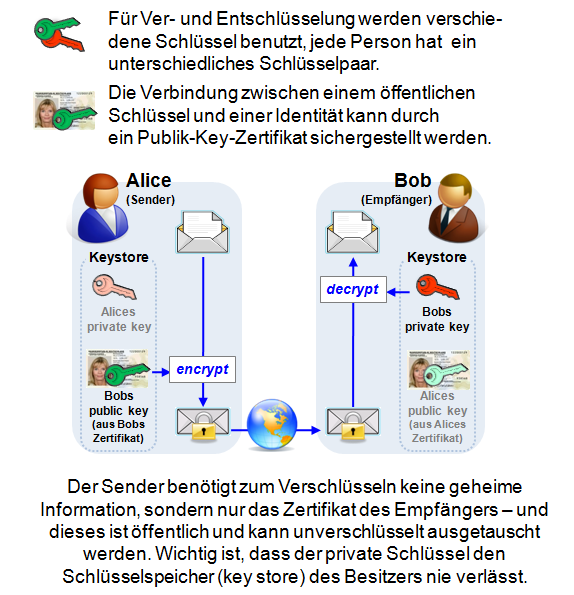
\includegraphics[scale=0.7]{figures/AsymmetricEnc_Figure_Chap1_de.png}
\caption{Asymmetrische oder Public-Key-Verschl�sselung} 
\label{cm_Figure_Asymmetric-Enc_Public-Key-Enc}
\end{center}
\end{figure}

M�chte Alice\index{Alice}%
\footnote{%
  Zur Beschreibung kryptographischer Protokolle werden den Teilnehmern
  oft Namen gegeben (vergleiche \cite[S. 23]{Schneier1996}). 
  Alice und Bob\index{Bob} f�hren alle allgemeinen 2-Personen-Protokolle durch,
  wobei Alice dies initiiert und Bob antwortet.
  Die Angreifer werden als Eve (eavesdropper = passiver Lauscher) und
  Mallory (malicious active attacker = b�swilliger, aktiver Abgreifer)
  bezeichnet.
  }
mit Bob kommunizieren, so sucht sie Bobs �ffentlichen Schl�ssel
und benutzt ihn, um ihre Nachricht an ihn zu
verschl�sseln. Diesen verschl�sselten Text schickt sie dann an Bob,
der mit Hilfe seines geheimen Schl�ssels den Text wieder entschl�s"-seln
kann. Da einzig Bob Kenntnis von seinem geheimen Schl�ssel hat, ist
auch nur er in der Lage, an ihn adressierte Nachrichten zu
entschl�sseln.
Selbst Alice als Absenderin der Nachricht kann aus der von ihr
versandten (verschl�sselten) Nachricht den Klartext nicht wieder
herstellen. Nat�rlich muss sichergestellt sein, dass man aus dem
�ffentlichen Schl�ssel nicht auf den geheimen Schl�ssel schlie�en
kann.\par \vskip + 3pt

% Abbildung evtl. besser hier, wenn Seitenaufteilung ausginge.

Veranschaulichen kann man sich ein solches Verfahren mit einer
Reihe von einbruchssicheren Briefk�sten. Wenn ich eine Nachricht
verfasst habe, so suche ich den Briefkasten\index{Briefkasten} mit dem
Namensschild des Empf�ngers und werfe den Brief dort ein. Danach kann ich die
Nachricht selbst nicht mehr lesen oder ver�ndern, da nur der
legitime Empf�nger im Besitz des Schl�ssels f�r den Briefkasten
ist.\par \vskip + 3pt

Vorteil von asymmetrischen Verfahren ist das einfachere
\index{Schl�sselmanagement} Schl�sselmanagement. Betrachten wir
wieder ein Netz mit $n$ Teilnehmern. Um sicherzustellen, dass
jeder Teilnehmer jederzeit eine verschl�sselte Verbindung zu
jedem anderen Teilnehmer aufbauen kann, muss jeder Teilnehmer ein
Schl�sselpaar besitzen. Man braucht also $2n$ Schl�ssel oder $n$
Schl�sselpaare. Ferner ist im Vorfeld einer �bertragung kein
sicherer Kanal notwendig, da alle Informationen, die zur Aufnahme
einer vertraulichen Kommunikation notwendig sind, offen
�bertragen werden k�nnen. Hier ist lediglich%
\footnote{%
Dass auch dies nicht trivial ist, wird z.B. in Kapitel \ref{nt_Shared-Primes}
erl�utert.
Neben den Anforderungen bei der Schl�sselgenerierung ist zu beachten, dass
inzwischen auch die (Public-Key-)Infrastrukturen selbst Ziel von 
Cyber-Angriffen sind.
}
auf die Unverf�lschtheit (Integrit�t und Authentizit�t)
\index{Authentizit�t} des �ffentlichen Schl�ssels zu achten.
Nachteil: Im Vergleich zu symmetrischen Verfahren sind reine
asymmetrische Verfahren jedoch um ein Vielfaches langsamer.\par \vskip + 3pt

Das bekannteste asymmetrische Verfahren ist der \index{RSA} 
RSA-Algorithmus\index{CrypTool}%
\footnote{%
  RSA wird in diesem Skript ab Kapitel \ref{rsabeweis} ausf�hrlich beschrieben.
  Die aktuellen Forschungsergebnisse im Umfeld von RSA werden in Kapitel
  \ref{SecurityRSA} beschrieben.
}%
, der nach seinen Entwicklern Ronald \index{Rivest, Ronald} Rivest, 
Adi \index{Shamir, Adi} Shamir und Leonard \index{Adleman, Leonard} Adleman
benannt wurde. Der RSA-Algorith"-mus wurde 1978 ver�ffentlicht.\footnote{%
  Hinweise zur Geschichte von RSA und seiner Ver�ffentlichung, die nicht im Sinne
  der NSA war, finden sich in der Artikelserie {\em RSA \& Co. in der Schule:
  Moderne Kryptologie, alte Mathematik, raffinierte Protokolle}.
  Siehe \cite{Witten2006}, S. 55 ff (\glqq Penible L�mmergeier\grqq).
  \index{RSA \& Co. in der Schule}
}
Das Konzept der asymmetrischen Verschl�sselung wurde erstmals
von Whitfield Diffie \index{Diffie, Whitfield}  und 
Martin \index{Hellman, Martin} Hellman in Jahre 1976 vorgestellt. 
Heute spielen auch die Verfahren nach
ElGamal \index{ElGamal, Tahir} eine bedeutende Rolle, vor allem die
\index{Schnorr, Claus-Peter} Schnorr-Varianten im \index{DSA} DSA (Digital
\index{Signatur!digital}\index{DSA-Signatur}\index{Signatur!DSA}
Signature Algorithm).

\noindent Angriffe gegen asymmetrische Verfahren werden behandelt in\\
- Kapitel~ \ref{Chapter_ElementaryNT}: \hyperlink{Chapter_ElementaryNT}{Elementare Zahlentheorie},\\
- Kapitel~ \ref{Chapter_ModernCryptography}:
  \hyperlink{Chapter_ModernCryptography}{Moderne Kryptographie},\\
- Kapitel~ \ref{Chapter_EllipticCurves}:
  \hyperlink{Chapter_EllipticCurves}{Elliptische Kurven} und\\
- Kapitel \ref{Chapter_Dlog-FactoringDead}: \hyperlink{Chapter_Dlog-FactoringDead}
  {Aktuelle Resultate zum L�sen diskreter Logarithmen und zur Faktorisierung}.



% --------------------------------------------------------------------------
\newpage
\section[Hybridverfahren]{Hybridverfahren\footnotemark} 
\footnotetext{%
   In CT1\index{CT1} finden Sie dieses Verfahren �ber das Men�
   {\bf Ver-/Entschl�sseln \textbackslash{} Hybrid}:
   Dabei k�nnen Sie die einzelnen Schritte und ihre Abh�ngigkeiten mit konkreten
   Zahlen nachvollziehen. Die Variante mit RSA als asymmetrischem Verfahren
   ist graphisch visualisiert; die Variante mit ECC nutzt die Standard-Dialoge.
   In beiden F�llen wird AES als symmetrisches Verfahren eingesetzt.\index{AES}\\
   JCT\index{JCT} bietet Hybrid-Verfahren (z.B. ECIES) in der
   Algorithmen-Perspektive an unter {\bf Algorithms \textbackslash{} Hybrid Ciphers}.
}
\label{CM_Hybrid-procedures}
\index{Hybridverfahren}

Um die Vorteile von symmetrischen und asymmetrischen Techniken gemeinsam 
nutzen zu k�nnen, werden (zur Verschl�sselung) in der Praxis meist 
Hybridverfahren \index{Verschl�sselung!hybrid} verwendet.\par \vskip + 3pt

Hier werden die Mengen-Daten mittels symmetrischer Verfahren
verschl�sselt: Der Schl�ssel ist ein vom Absender zuf�llig\footnote{%
   Die Erzeugung zuf�lliger Zahlen\index{Zufall} ist ein wichtiger Bestandteil 
   kryptographisch sicherer Verfahren.\\
   - Mit CT1\index{CT1} k�nnen Sie �ber das Men�
   {\bf Einzelverfahren \textbackslash{} Zufallsdaten erzeugen}
   verschiedene Zufallszahlengeneratoren\index{Zufallsgenerator} (PRNGs) ausprobieren.
   �ber das Men� {\bf Analyse \textbackslash{} Zufallsanalyse} k�nnen Sie
   verschiedene Testverfahren f�r Zufallsdaten auf bin�re Dokumente
   anwenden.\\
   % CT1 konzentriert sich auf kryptographisch starke
   % {\bf Pseudo}zufallszahlengeneratoren. \glqq Echte\grqq~
   % Zufallsquellen werden nur �ber den Aufruf des Secude-Generators einbezogen.\\
   %
   - In CT2\index{CT2} k�nnen Sie im Startcenter
   mit dem Suchstring \glqq Zufall\grqq~Vorlagen (Templates) finden, die
   Zufallsgeneratoren\index{Zufallsgenerator} (PRNGs)
   nutzen. Die PRNGs nutzen intern bspw. Keccak\index{Keccak} oder den
   Linear Congruential Generator (LCG)\index{LCG}. Sie werden dann
   bspw. f�r Schl�sselgenerierung oder Dezimalisierung genutzt.\\
   %
   - JCT\index{JCT} bietet {\bf Pseudo}zufallszahlengeneratoren sowohl
   im Men� {\bf Algorithms \textbackslash{} Random Number Generator} der
   Standard-Perspektive als auch in der Algorithmen-Perspektive an.
}\index{Zufall}
generierter geheimer Sitzungsschl�ssel (session key)\index{Session Key},
der nur f�r diese Nachricht verwendet wird.

Anschlie�end wird dieser Sitzungsschl�ssel mit Hilfe des asymmetrischen
Verfahrens verschl�sselt und zusammen mit der Nachricht an den Empf�nger
�bertragen.

Der Empf�nger kann den Sitzungsschl�ssel mit Hilfe seines geheimen
Schl�ssels bestimmen und mit diesem dann die Nachricht entschl�sseln.

Auf diese Weise profitiert man von dem bequemen Schl�sselmanagement\index{Schl�sselmanagement}
asymmetrischer Verfahren (mit �ffentlichem und privatem Schl�ssel), und
man profitiert von der Schnelligkeit symmetrischer Verfahren, um gro�e
Datenmengen zu verschl�sseln (mit den geheimen Schl�sseln).



% --------------------------------------------------------------------------
\newpage
% \vskip +40 pt

\begin{ctsquote}
    Ein altes Sprichwort, angeblich gepr�gt von der
    US National Security Agency (NSA), sagt:\\
    \glqq Angriffe werden immer besser, niemals schlechter.\grqq\\
    ``Attacks always get better; they never get worse.''
\caption[IETF]{IETF\footnotemark}
\end{ctsquote}
\addtocounter{footnote}{0}\footnotetext{%
  \url{http://tools.ietf.org/html/rfc4270}\index{IETF}\index{NSA}
  }

% --------------------------------------------------------------------------
\section[Kryptoanalyse und symmetrische Chiffren f�r Lehrzwecke]{Kryptoanalyse und symmetrische Chiffren f�r Lehrzwecke\footnotemark} 
\footnotetext{%
  Ein sehr guter Start in die Kryptoanalyse ist das Buch von Mark Stamp \cite{Stamp2007}.
  Ebenfalls gut, aber sehr high-level und nur bezogen auf die Analyse symmetrischer
  Blockchiffren ist der Artikel von Bruce Schneier \cite{Schneier2000}.\\
  Einige der Cipher-Challenges bei \glqq MysteryTwister C3\grqq~
  (\url{http://www.mysterytwisterc3.org}) sind ebenfalls gut f�r Lehrzwecke
  einsetzbar.\index{MTC3}\index{Krypto-Wettbewerb}
}
\label{CM_Analysis-SymCiphers-Educational}
\index{Kryptoanalyse}

Verglichen mit den auf der Zahlentheorie beruhenden Public-Key-Verschl�sselungsverfahren wie RSA, ist die Struktur von AES\index{AES} und den meisten anderen modernen symmetrischen Verschl�sse"-lungsverfahren (wie DES, IDEA oder Present) sehr komplex und kann nicht so einfach wie RSA\index{RSA} erkl�rt werden.

Deshalb wurden zu Lehrzwecken vereinfachte Varianten moderner
symmetrischer Verfahren entwickelt, um Einsteigern die M�glichkeit zu geben,
Ver- und Entschl�sselung von Hand zu lernen und ein besseres Verst�ndnis zu
gewinnen, wie die Algorithmen im Detail funktionieren.
Diese vereinfachten Varianten helfen auch, die entsprechenden
Kryptoanalyse-Methoden zu verstehen und anzuwenden.

Die bekanntesten Varianten sind SDES (Simplified DES)%
\footnote{
  Visualisierung: Macht man in CT2\index{CT2} einen Doppelklick auf den Titel der
  SDES-Komponente, ist in der Fullscreen-Ansicht
  % fullscreen
  % in der Fullscreen-Ansicht  %% das gab eine Zeile zuviel und r�ckte 1.7. weiter.
  zu sehen, wie die Bits der eingegebenen Daten durch den Algorithmus flie�en.
  Ein Screen\-shot dazu:
  \url{https://www.facebook.com/CrypTool2/photos/a.505204806238612.1073741827.243959195696509/597354423690316}
}
und S-AES (Simplified-AES) von Prof. Ed Schaefer und seinen Studenten%
\footnote{
    Siehe auch den Artikel \glqq Devising a Better Way to Teach and Learn
    the Advanced Encryption Standard\grqq~unter
    \url{http://math.scu.edu/~eschaefe/getfile.pdf}
    % be_2016-07-17: dead link /toter Link: http://www.scu.edu/cas/research/cryptography.cfm
},
und Mini-AES (siehe das Kapitel~\ref{CM_Sage_Mini-AES} \glqq \nameref{CM_Sage_Mini-AES}\grqq):

\index{DES}\index{DES!SDES}\index{IDEA}\index{AES!Mini-AES}\index{AES!S-AES}
\begin{itemize}

\item Edward F. Schaefer: {\em A Simplified Data Encryption Standard Algorithm} 
      \cite{Schaefer1996}.

\item Raphael Chung-Wei Phan: {\em Mini Advanced Encryption Standard (Mini-AES):
                                   A Testbed for Cryptanalysis Students} 
      \cite{Phan2002}.

\item Raphael Chung-Wei Phan: {\em Impossible differential cryptanalysis of Mini-AES} 
      \cite{Phan2003}.

\item Mohammad A. Musa, Edward F. Schaefer, Stephen Wedig:
      {\em A simplified AES algorithm and its linear and differential cryptanalyses} 
      \cite{Musa2003}.

\item Nick Hoffman: {\em A SIMPLIFIED IDEA ALGORITHM} 
      \cite{Hoffman2006}.

\item S. Davod. Mansoori, H. Khaleghei Bizaki: 
      {\em On the vulnerability of Simplified AES Algorithm Against Linear Cryptanalysis} 
      \cite{Mansoori2007}.

\end{itemize}



% --------------------------------------------------------------------------
\section{Weitere Informationsquellen}

Neben den anderen Kapiteln in diesem Skript, der umfangreichen Fachliteratur
und vielen Stellen im Internet enth�lt auch die Online-Hilfe aller 
CrypTool-Varianten\index{CrypTool} sehr viele weitere Informationen zu den 
einzelnen symmetrischen und asymmetrischen Verschl�sselungsverfahren.




% ---------------------------------------------------------------------------
% ---------------------------------------------------------------------------
\newpage
\hypertarget{CM_Appendix_SageCode}{}
\section{Anhang: Beispiele mit SageMath}
\label{CM_Sage_samples}
\index{SageMath!Programmbeispiele}

\noindent Der folgende Abschnitt enth�lt SageMath Source-Code, der sich auf den
Inhalt des Kapitels~\ref{CM_Analysis-SymCiphers-Educational}
(\glqq \nameref{CM_Analysis-SymCiphers-Educational}\grqq) bezieht.

Weitere Details zu in SageMath enthaltenen Kryptoverfahren (z.B. zum Simplified
Data Encryption Standard SDES) finden sich z.B. in der Diplomarbeit von Minh Van
Nguyen \cite{Nguyen2009b}.

% ---------------------------------------------------------------------------
\subsection{Mini-AES}
\label{CM_Sage_Mini-AES}
\index{AES!Mini-AES}

Das SageMath-Modul \texttt{crypto/block\_cipher/miniaes.py} enth�lt den Mini-AES, mit
dem Studenten die Funktionsweise moderner Blockchiffren untersuchen k�nnen.

Mini-AES, urspr�nglich vorgestellt von \cite{Phan2002}, ist eine vereinfachte
Variante des Advanced Encryption Standard (AES) f�r Ausbildungszwecke.

Wie man Mini-AES benutzt, ist ausf�hrlich in der SageMath Reference-Page beschrieben:
\begin{sloppypar} % N�tig, da sonst ein schwarzer Punkt
  \url{http://doc.sagemath.org/html/en/reference/cryptography/sage/crypto/block_cipher/miniaes.html}.
\end{sloppypar}

Das folgende SageMath-Code-Beispiel~\ref{cm_Mini-AES:Sage_example}
ist aus den Release-Notes von SageMath 4.1%
\footnote{
  Siehe \url{http://mvngu.wordpress.com/2009/07/12/sage-4-1-released/}.\\
  Weiterer Beispiel-Code zum Mini-AES findet sich in
  \cite[Kap. 6.5 und Anhang D]{Nguyen2009a}.
}
und ruft diese Implementierung des Mini-AES auf.


% Using [fontsize=\footnotesize,fontshape=tt] caused:
%   LaTeX Font Warning: Font shape `T1/cmtt/m/tt' undefined
%   (Font)              using `T1/cmtt/m/n' instead on input line 730.
% so deleted the fontshape parameter.
\begin{sagecode}
\begin{Verbatim}%
[fontsize=\footnotesize]
# We can encrypt a plaintext using Mini-AES as follows:
sage: from sage.crypto.block_cipher.miniaes import MiniAES
sage: maes = MiniAES()
sage: K = FiniteField(16, "x")
sage: MS = MatrixSpace(K, 2, 2)
sage: P = MS([K("x^3 + x"), K("x^2 + 1"), K("x^2 + x"), K("x^3 + x^2")]); P

[  x^3 + x   x^2 + 1]
[  x^2 + x x^3 + x^2]
sage: key = MS([K("x^3 + x^2"), K("x^3 + x"), K("x^3 + x^2 + x"), K("x^2 + x + 1")]); key

[    x^3 + x^2       x^3 + x]
[x^3 + x^2 + x   x^2 + x + 1]
sage: C = maes.encrypt(P, key); C

[            x       x^2 + x]
[x^3 + x^2 + x       x^3 + x]

# Here is the decryption process:
sage: plaintxt = maes.decrypt(C, key)
sage: plaintxt == P
True

# We can also work directly with binary strings:
sage: from sage.crypto.block_cipher.miniaes import MiniAES
sage: maes = MiniAES()
sage: bin = BinaryStrings()
sage: key = bin.encoding("KE"); key
0100101101000101
sage: P = bin.encoding("Encrypt this secret message!")
sage: C = maes(P, key, algorithm="encrypt")
sage: plaintxt = maes(C, key, algorithm="decrypt")
sage: plaintxt == P
True

# Or work with integers n such that 0 <= n <= 15:
sage: from sage.crypto.block_cipher.miniaes import MiniAES
sage: maes = MiniAES()
sage: P = [n for n in xrange(16)]; P
[0, 1, 2, 3, 4, 5, 6, 7, 8, 9, 10, 11, 12, 13, 14, 15]
sage: key = [2, 3, 11, 0]; key
[2, 3, 11, 0]
sage: P = maes.integer_to_binary(P)
sage: key = maes.integer_to_binary(key)
sage: C = maes(P, key, algorithm="encrypt")
sage: plaintxt = maes(C, key, algorithm="decrypt")
sage: plaintxt == P
True
\end{Verbatim}
\caption{Ver- und Entschl�sselung mit dem Mini-AES}
\label{cm_Mini-AES:Sage_example}
\end{sagecode}
\clearpage%% Um das Codebeispiel vor das ff. Kap. 1.8.2 zu bekommen.


% ---------------------------------------------------------------------------
\subsection{Weitere symmetrische Krypto-Algorithmen in SageMath}
\label{CM_Sage_SymCryptoAlg}

Die Referenz zu SageMath v7.2 f�hrt als kryptographische Funktionen u.a. auf:%
\footnote{
  Siehe 
  \url{http://doc.sagemath.org/html/en/reference/sage/crypto/index.html},\\
  \url{http://doc.sagemath.org/html/en/reference/cryptography/index.html} und\\
  \url{http://combinat.sagemath.org/doc/reference/cryptography/sage/crypto/stream.html}
}
\begin{itemize}
   \item Linear feedback shift register (LFSR),
   \item Blum-Blum-Shub (BBS): Pseudo-Zufallsbit-Generator (zu finden bei Streams),
   \item Gitter-basierte Funktionen.
% be_2016-07-17: Nicht mehr gefunden in Refrence 7.2:
% - ShrinkingGeneratorCryptosystem,
\end{itemize}



%------------------------------------------------------------------------------
\putbib[../de/references]
\addcontentsline{toc}{section}{Literaturverzeichnis}
\end{bibunit}

\noindent Alle Links wurden am 10.07.2016 �berpr�ft.



% --------------------------------------------------------------------------
\newpage
\chapter*{Web-Links}\addcontentsline{toc}{section}{Web-Links}

\begin{enumerate}

  \hypertarget{CM_HT_Weblink_Rijndael-Cryptosystem}{}
  \item \glqq AES Discussion Groups\grqq~beim NIST (archive page provided for historical purposes, last update on Feb 28th, 2001)\\
	% \grqq nach \item braucht die Tilde, aber kein weiteres Blank.
	%  Sonst reicht ein Blank, wenn ein weiteres Wort danach folgt
	%  (es reicht auch nicht, wenn danach ein Zeilenumbruch).
	\url{http://csrc.nist.gov/archive/aes/}

  \item Das AES-/Rijndael-Kryptosystem (page maintained by Nicolas T. Courtois, last update on Aug 24th, 2007)\\
        \url{http://www.cryptosystem.net/aes}

  \item distributed.net:~\glqq RC5-64 has been solved\grqq\\
        \url{http://www.distributed.net/Pressroom_press-rc5-64}

	% \begin{sloppypar}  ... \end{sloppypar} worked. Get rid of \\ before to avoid extra newline.
\item RSA Labs (ehemals RSA Security): ~\glqq The RSA Secret Key Challenge\grqq
        \begin{sloppypar}
	\url{https://www.emc.com/emc-plus/rsa-labs/historical/the-rsa-laboratories-secret-key-challenge.htm}
	\end{sloppypar}

  \item RSA Labs (ehemals RSA Security): ~\glqq DES Challenge\grqq\\
        \url{https://www.emc.com/emc-plus/rsa-labs/historical/des-challenge-iii.htm}

  \item Weiterf�hrende Links auf der CrypTool-Homepage\\
        \url{http://www.cryptool.org}
	       
\end{enumerate}

Alle Links wurden am 10.07.2016 �berpr�ft.



% Local Variables:
% TeX-master: "../script-de.tex"
% End:

\renewcommand{\CTBChapName}{(Chap PaP)}           % $Id$
% ............................................................................
%             V E R S C H L U E S S E L U N G S V E R F A H R E N
% ~~~~~~~~~~~~~~~~~~~~~~~~~~~~~~~~~~~~~~~~~~~~~~~~~~~~~~~~~~~~~~~~~~~~~~~~~~~~
% "`xx"'
\newpage
\hypertarget{Kapitel_PaperandPencil}{}

\chapter{Papier- und Bleistift-Verschl�sselungsverfahren}
\label{Kapitel_PaperandPencil}
(Christine St�tzel, April 2004; Updates B.+C. Esslinger, Juni 2005; Updates Minh Van Nguyen und B. Esslinger, Juli 2009)
\index{Papier- und Bleistiftverfahren}

\begin{center}
\fbox{\parbox{15cm}{%
{\em Edgar Allan Poe\index{Poe, Edgar Allan}: 
A Few Words on Secret Writing, 1841}\\
Nur Wenige kann man glauben machen, dass es keine leichte Sache ist,
eine Geheimschrift zu erdenken, die sich der Untersuchung widersetzt.
Dennoch kann man rundheraus annehmen, dass menschlicher Scharfsinn
keine Chiffre erdenken kann, die menschlicher Scharfsinn nicht l�sen kann.}}
\end{center}

Das folgende Kapitel bietet einen recht vollst�ndigen �berblick �ber Papier- 
und Bleistiftverfahren\footnote{%
In den Fu�noten zu diesem Kapitel wird jeweils
beschrieben, wie man diese Verfahren mit CrypTool 1 ausf�hren kann.
Au�erdem enth�lt das letzte Unterkapitel (\ref{PaP_Sage_samples})
zu einigen Verfahren Beispielcode in dem Computer-Algebra-System Sage\index{Sage}.
                               }.
Unter diesem Begriff lassen sich alle Verfahren zusammenfassen, die Menschen von
Hand anwenden k�nnen, um Nachrichten zu ver- und entschl�sseln.
Besonders popul�r waren diese Verfahren f�r Geheimdienste (und 
sind es immer noch), da ein Schreibblock und ein Stift -- im 
Gegensatz zu elektronischen Hilfsmitteln -- vollkommen unverd�chtig sind.

Die ersten Papier- und Bleistiftverfahren entstanden bereits vor rund 
3000 Jahren, aber auch w�hrend des vergangenen Jahrhunderts kamen 
noch zahlreiche neue Methoden hinzu. Bei allen Papier- und 
Bleistiftverfahren handelt es sich um symmetrische
Verfahren\index{Verschl�sselung!symmetrisch}. Selbst in den 
�ltesten Verschl�sselungsmethoden steckten schon die
grunds�tzlichen Konstruktionsprinzipien wie Transposition, 
Substitution, Blockbildung und deren Kombination. Daher
lohnt es sich vor allem aus didaktischen Gesichtspunkten, 
diese "`alten"' Verfahren genauer zu betrachten.

Erfolgreiche bzw. verbreiteter eingesetzte Verfahren mussten die gleichen 
Merkmale erf�llen wie moderne Verfahren:
\begin{itemize}
\item Vollst�ndige Beschreibung, klare Regeln, ja fast Standardisierung 
      (inkl. der Sonderf�lle, dem Padding, etc.).
\item Gute Balance zwischen Sicherheit und Benutzbarkeit 
      (denn zu kompliziert zu bedienende Verfahren waren fehlertr�chtig
      oder unangemessen langsam).
\end{itemize}


\newpage
%------------------------------------------------------------------------------
\section{Transpositionsverfahren}
\label{PaP_transposition_ciphers}
\index{Transposition}

Bei der Verschl�sselung durch Transposition\index{Transposition} 
bleiben die urspr�nglichen Zeichen der Nachricht erhalten,
nur ihre Anordnung wird ge�ndert (Transposition = 
Vertauschung)\footnote{Ein anderer Begriff f�r eine Transposition
ist Permutation\index{Permutation}.}.

%------------------------------------------------------------------------------
\subsection{Einf�hrungs-Beispiele unterschiedlicher
               Transpositionsverfahren}
\label{introsamplesTranspositionCiphers}  %be_2006 so ist es gut.

\begin{itemize}

\item {\bf Gartenzaun}\footnote{%
   Dieses Verfahren kann direkt in CrypTool\index{CrypTool} mit dem Men�punkt 
   {\bf Ver-/Entschl�sseln \textbackslash{} Symmetrisch (klassisch) \textbackslash{}
   Skytale / Gartenzaun} abgebildet werden.
   Man kann diese Matheode auch simulieren �ber den Men�eintrag {\bf Ver-/Entschl�sseln
   \textbackslash{} Symmetrisch (klassisch) \textbackslash{} Permutation}:
   f�r einen Gartenzaun mit 2 Zeilen gibt man als Schl�ssel
   "`B,A"' ein und l�sst ansonsten die Standardeinstellungen (nur 1
   Permutation, in der man zeilenweise ein- und spaltenweise ausliest). 
   Mit dem Schl�ssel "`A,B"' w�rde man man das Zick-zack-Muster unten so 
   beginnen, dass der 1. Buchstabe in der ersten statt in der 2. Zeile steht.}
   \cite{Singh2001}\index{Gartenzaun-Verschl�sselung}:
                        % Kein Blank VOR "\index", sonst ist der
                        % Doppelpunkt nicht direkt nach dem Fussnotenindex.
   Die Buchstaben des Klartextes werden abwechselnd in zwei (oder mehr) 
   Zeilen geschrieben, so dass ein Zickzack-Muster entsteht. 
   Dann werden die Zeichen zeilenweise nacheinander gelesen.\\
   Dieses Verfahren ist eher eine Kinderverschl�sselung.
	
   Klartext\footnote{Wenn das Alphabet nur die 26 Buchstaben verwendet, 
   schreiben wir den Klartext in Kleinbuchstaben und den Geheimtext in 
   Gro�buchstaben.}: ein beispiel zur transposition

   \begin{table}[h]
   \begin{center}
   \begin{tabular}{r@{\:}r@{\:}r@{\:}r@{\:}r@{\:}r@{\:}r@{\:}r@{\:}r@{\:}
                r@{\:}r@{\:}r@{\:}r@{\:}r@{\:}r@{\:}r@{\:}r@{\:}r@{\:}
                r@{\:}r@{\:}r@{\:}r@{\:}r@{\:}r@{\:}r@{\:}r@{\:}r@{\:}}
	  & i &   & b &   & i &   & p &   & e &   & z &   & r &   & 
            r &   & n &   & p &   & s &   & t &   & o &   \\
	e &   & n &   & e &   & s &   & i &   & l &   & u &   & t &
          & a &   & s &   & o &   & i &   & i &   & n 
   \end{tabular}
   \caption{Gartenzaun-Verschl�sselung}
   \end{center}
   \end{table}

   Geheimtext\footnote{Die Buchstaben des Klartextes sind hier -- wie 
   historisch �blich -- in 5-er Bl�cken gruppiert. Man k�nnte o.E.d.A.
   auch eine andere (konstante) Blockl�nge oder gar keine Trennung durch 
   Leerzeichen w�hlen.}%
   : IBIPE ZRRNP STOEN ESILU TASOI IN\\


\item {\bf Skytale von Sparta}\footnote{%
   Dieses Verfahren kann direkt in CrypTool\index{CrypTool} mit dem Men�punkt 
   {\bf Ver-/Entschl�sseln \textbackslash{} Symmetrisch (klassisch) \textbackslash{}
   Skytale / Gartenzaun} abgebildet werden.
   Da dieses Verschl�sselungsverfahrens ein Spezialfall der einfachen
   Spaltentransposition ist, kann man es in CrypTool\index{CrypTool} simulieren
   �ber den Men�eintrag {\bf Ver-/Entschl�sseln \textbackslash{} Symmetrisch (klassisch) 
   \textbackslash{} Permutation}: F�r die Skytale braucht man in
   der Dialogbox nur die erste Permutation. Darin gibt man bei z.B. 4 
   Kanten als Schl�ssel  "`1,2,3,4"'  ein. Dies w�re so, als w�rde man
   den Text in 4-er Bl�cken waagrecht in eine Tabelle schreiben und 
   senkrecht auslesen. 
   Weil der Schl�ssel aufsteigend geordnet ist, bezeichnet man die Skytale
   auch als identische Permutation. Weil das Schreiben und Auslesen nur 
   einmal durchgef�hrt wird, als einfache (und nicht als doppelte)
   Permutation.}
   \cite{Singh2001}\index{Skytale}%
   : 
   Dieses Verfahren wurde wahrscheinlich das erste Mal um 600 v.Chr.
   benutzt und es wurde von dem griechischen Schriftsteller und Philosophen
   Plutarch (50-120 v.Chr.) zuerst beschrieben.\\
   Um einen Holzstab wird ein Streifen Papier o.�. gewickelt. Dann wird
   darauf zeilenweise der Klartext geschrieben. 
   Wickelt man den Streifen ab, h�lt man den Geheimtext in den H�nden.

\item {\bf Schablone} \cite{Goebel2003}: Sender und Empf�nger benutzen
   die gleiche Schablone. In deren L�cher werden zeilenweise die
   Klartextzeichen geschrieben, die dann spaltenweise ausgelesen werden. 
   Bleibt Klartext �brig, wird der Vorgang wiederholt, unter Umst�nden 
   mit einer anderen Ausrichtung der Schablone\footnote{%
   Dieses Verfahren kann man nicht durch eine einfache Spaltentransposition
   darstellen.}.

   \hypertarget{turning-grille}{}  %be_2006 so ist es gut.
\item {\bf Flei�ner-Schablone} \cite{Savard1999}% verhindert, dass Blank vor ":"
   \index{Flei�ner-Schablone}: 
   Die Flei�ner-Schablone
   wurde im Ersten Weltkrieg von deutschen Soldaten benutzt\footnote{%
   Erfunden wurde die Flei�ner-Schablone bereits 1881 von Eduard Flei�ner
   von Wostrowitz.\\
   Eine gute Visualisierung findet sich unter www.turning-grille.com.}%
   .
   Ein quadratisches Gitter dient als Schablone, wobei ein Viertel der 
   Felder L�cher hat. Der erste Teil des Klartextes wird zeichenweise 
   durch die L�cher auf ein Blatt Papier geschrieben, dann wird die
   Schablone um 90 Grad gedreht, und der zweite Teil des Textes wird
   auf das Papier geschrieben, usw. Die Kunst besteht in der richtigen 
   Wahl der L�cher: Kein Feld auf dem Papier darf frei bleiben, es 
   darf aber auch keines doppelt beschriftet werden. Der Geheimtext 
   wird zeilenweise ausgelesen.

   In die Beispiel-Flei�ner-Schablone in der folgenden Tabelle k�nnen
   4 Mal je 16 Zeichen des Klartextes auf ein Blatt geschrieben werden:
   \begin{table}[h]
   \begin{center}
   \begin{tabular}{|cccc|cccc|}
   \hline 	
	O & - & - & - & - & O & - & - \\
	- & - & - & O & O & - & - & O \\
	- & - & - & O & - & - & O & - \\
	- & - & O & - & - & - & - & - \\
   \hline 	
	- & - & - & - & O & - & - & - \\
	O & - & O & - & - & - & O & - \\
	- & O & - & - & - & - & - & O \\
	- & - & - & O & O & - & - & - \\
   \hline
   \end{tabular}  
   \caption{8x8-Flei�ner-Schablone}
   \end{center} 
   \end{table}

\end{itemize}


%------------------------------------------------------------------------------
\subsection[Spalten- und Zeilentranspositionsverfahren]
    {Spalten- und Zeilentranspositionsverfahren\footnotemark}
    \footnotetext{%
Die meisten der folgenden Verfahren k�nnen in CrypTool\index{CrypTool}
mit dem Men�punkt {\bf Ver-/Entschl�sseln \textbackslash{} 
Symmetrisch (klassisch) \textbackslash{} Permutation} abgebildet werden.}

\begin{itemize}

\item {\bf Einfache Spaltentransposition} \cite{Savard1999}: Zun�chst wird
   ein Schl�sselwort bestimmt, das �ber die Spalten eines Gitters geschrieben
   wird. Dann schreibt man den zu verschl�sseln"-den Text zeilenweise in dieses
   Gitter.
   Die Spalten werden entsprechend des Auftretens der Buchstaben des 
   Schl�sselwortes im Alphabet durchnummeriert. In dieser Reihenfolge werden 
   nun auch die Spalten ausgelesen und so der Geheimtext gebildet\footnote{%
   Darstellung mit CrypTool: Eingabe eines Schl�ssels f�r die 1. Permutation,
   zeilenweise einlesen, spaltenweise permutieren und auslesen.}.
	
   Klartext: ein beispiel zur transposition

   \begin{table}[h]
   \begin{center}
   \begin{tabular}{|c|c|c|}
   \hline
	K & E & Y \\
   \hline
	e & i & n \\
	b & e & i \\
	s & p & i \\
	e & l & z \\
	u & r & t \\
	r & a & n \\
	s & p & o \\
	s & i & t \\
	i & o & n \\
   \hline
   \end{tabular}
   \caption{Einfache Spaltentransposition}
   \end{center}
   \end{table}

   Transpositionsschl�ssel: K=2; E=1; Y=3. \\
   Geheimtext: IEPLR APIOE BSEUR SSINI IZTNO TN \\

\item {\bf AMSCO} \cite{ACA2002}\index{AMSCO}: Die Klartextzeichen werden 
   abwechselnd in Einer- und Zweiergruppen in ein Gitter geschrieben.
   Dann erfolgt eine Vertauschung der Spalten, anschlie�end das Auslesen.

\item {\bf Doppelte Spaltentransposition / "`Doppelw�rfel"'} 
   \cite{Savard1999}\index{Doppelw�rfel}: 
   Die doppelte 
   Spaltentransposition wurde h�ufig im Zweiten Weltkrieg und zu Zeiten des 
   Kalten Krieges angewendet. Dabei werden zwei Spaltentranspositionen 
   nacheinander durchgef�hrt, f�r die zweite Transposition wird ein neuer
   Schl�ssel benutzt\footnote{%
   Darstellung mit CrypTool: Eingabe eines Schl�ssels f�r die 1. Permutation,
   zeilenweise einlesen, spaltenweise permutieren und auslesen.
   Eingabe eines (neuen) Schl�ssels f�r die 2. Permutation, Ergebnis der
   1. Permutation zeilenweise einlesen, spaltenweise permutieren und
   auslesen.}.

\item {\bf Spaltentransposition, General Luigi Sacco} \cite{Savard1999}: Die 
   Spalten eines Gitters werden den Buchstaben des Schl�sselwortes
   entsprechend nummeriert. Der Klartext wird dann zeilenweise eingetragen,
   in der ersten Zeile bis zur Spalte mit der Nummer 1, in der zweiten Zeile
   bis zur Spalte mit der Nummer 2 usw. Das Auslesen erfolgt wiederum
   spaltenweise.

   Klartext: ein beispiel zur transposition

   \begin{table}[h]
   \begin{center}
   \begin{tabular}{|c|c|c|c|c|c|c|}
   \hline
	G & E & N & E & R & A & L\\
	4 & 2 & 6 & 3 & 7 & 1 & 5\\
   \hline
	e & i & n & b & e & i &  \\
	s & p &   &   &   &   &  \\
	i & e & l & z &   &   &  \\
	u &   &   &   &   &   &  \\
	r & t & r & a & n & s & p\\
	o & s & i &   &   &   &  \\
	t & i & o & n &   &   &  \\
   \hline
   \end{tabular}
   \caption{Spaltentransposition nach General Luigi Sacco}
   \end{center}
   \end{table}

   Geheimtext: ESIUR OTIPE TSINL RIOBZ ANENI SP\\


\item {\bf Spaltentransposition, Franz�sische Armee im Ersten Weltkrieg}
   \cite{Savard1999}: 
   Nach Durch"-f�hrung einer Spaltentransposition werden diagonale Reihen
   ausgelesen.


\item {\bf Zeilentransposition} \cite{Savard1999}: Der Klartext wird in gleich 
   lange Bl�cke zerlegt, was auch mit Hilfe eines Gitters erfolgen kann. Dann
   wird die Reihenfolge der Buchstaben bzw. der Spalten vertauscht. Da das 
   Auslesen zeilenweise erfolgt, wird nur jeweils innerhalb der Bl�cke 
   permutiert\footnote{%
   Darstellung mit CrypTool: Eingabe eines Schl�ssels f�r die 1. Permutation, 
   zeilenweise einlesen, spaltenweise permutieren und zeilenweise auslesen.}.

\end{itemize}
% Ende \subsection{Spalten- und Zeilentranspositionsverfahren}



%------------------------------------------------------------------------------
\subsection{Weitere Transpositionsverfahren}

\begin{itemize}

\item {\bf Geometrische Figuren} \cite{Goebel2003}: Einem bestimmten Muster
   folgend wird der Klartext in ein Gitter geschrieben (Schnecke, R�sselsprung
   o.�.), einem zweiten Muster folgend wird der Geheimtext ausgelesen.

\item {\bf Union Route Cipher} \cite{Goebel2003}: Die Union Route Cipher hat 
   ihren Ursprung im Amerikanischen B�rgerkrieg. Nicht die Buchstaben einer
   Nachricht werden umsortiert, sondern die W�rter. F�r besonders pr�gnante 
   Namen und Bezeichnungen gibt es Codew�rter, die zusammen mit den Routen
   in einem Codebuch festgehalten werden. Eine Route bestimmt die Gr��e des
   Gitters, in das der Klartext eingetragen wird und das Muster, nach dem der
   Geheimtext ausgelesen wird. Zus�tzlich gibt es eine Anzahl von
   F�llw�rtern.

\item {\bf Nihilist-Transposition} \cite{ACA2002}%
   \index{Nihilist-Transposition}: 
   Der Klartext wird in eine
   quadratische Matrix eingetragen, an deren Seiten jeweils der gleiche 
   Schl�ssel steht. Anhand dieses Schl�ssels werden sowohl die Zeilen als 
   auch die Spalten alphabetisch geordnet und der Inhalt der Matrix
   dementsprechend umsortiert. Der Geheimtext wird zeilenweise ausgelesen.

   Klartext: ein beispiel zur transposition

   \begin{table}[h]
   \begin{center}
   \begin{tabular}{|c|ccccc||cc|ccccc|}
   \hline
	  & K & A & T & Z & E &   &   & A & E & K & T & Z\\
   \hline
	K & e & i & n & b & e &   & A & s & e & i & p & i\\
	A & i & s & p & i & e &   & E & s & i & o & i & t\\
	T & l & z & u & r & t &   & K & i & e & e & n & b\\
	Z & r & a & n & s & p &   & T & z & t & l & u & r\\
	E & o & s & i & t & i &   & Z & a & p & r & n & s\\
   \hline
   \end{tabular}
   \caption[Nihilist-Transposition]{Nihilist-Transposition\footnotemark}
   \end{center}
   \end{table}

   Geheimtext: SEIPI SIOIT IEENB ZTLUR APRNS\\
   \footnotetext{%
   Der linke Block ist das Resultat nach dem Einlesen. Der rechte Block ist 
   das Resultat nach dem Vertauschen von Zeilen und Spalten.}


\item {\bf Cadenus} \cite{ACA2002}\index{Cadenus}:
   Hierbei handelt es sich um eine 
   Spalten"-transposition, die zwei Schl�s"-sel"-worte benutzt.\\
   Das erste Schl�sselwort wird benutzt, um die Spalten zu vertauschen.\\
   Das zweite Schl�sselwort wird benutzt, um das Startzeichen jeder Spalte
   festzulegen: dieses zweite Schl�sselwort ist eine beliebige Permutation
   des benutzten Alphabets. Diese schreibt man links vor die erste Spalte.
   Jede Spalte wird dann vertikal so verschoben (wrap-around), dass sie mit dem
   Buchstaben beginnt, der in derjenigen Zeile, wo der Schl�sselbuchstabe des
   ersten Schl�sselwortes in dem zweiten Schl�sselwort zu finden ist.\\
   Der Geheimtext wird zeilenweise ausgelesen.

   Siehe Tabelle \ref{Cadenus-table-reference}.

   Klartext: ein laengeres beispiel zur transposition mit cadenus

   \begin{table}[h]
   \begin{center}
   \begin{tabular}{|c|ccc|ccc|ccc|}
   \hline
	  & K & {\bf E} & Y & {\bf E} & K & Y & {\bf E} & K & Y\\
   \hline
	A & e & i & n & i & e & n & {\bf p} & r & n\\
	D & l & a & e & a & l & e & i & b & o\\
	X & n & g & e & g & n & e & o & s & t\\
	K & r & e & s & e & {\bf r} & s & i & e & n\\
	C & b & e & i & e & b & i & a & u & t\\
	W & s & p & i & p & s & i & n & r & d\\
	N & e & l & z & l & e & z & i & s & u\\
	S & u & r & t & r & u & t & a & s & n\\
	Y & r & a & n & a & r & {\bf n} & g & i & e\\
	{\bf E} & s & {\bf p} & o & {\bf p} & s & o & e & m & e\\
	D & s & i & t & i & s & t & e & c & s\\
	T & i & o & n & o & i & n & p & e & i\\	
	U & m & i & t & i & m & t & l & s & i\\
	B & c & a & d & a & c & d & r & e & z\\
	R & e & n & u & n & e & u & a & l & t\\
	G & s & - & - & - & s & - & - & n & -\\
   \hline
   \end{tabular}
%be_2005: Fu�note zur Tabellen�berschrift wird nur angezeigt, wenn man das
%         \footnotetext-Statement nicht direkt hinter \caption{...} schreibt,
%         sondern au�erhalb!
%\caption{Cadenus\footnotemark}
   \caption[Cadenus]{Cadenus\footnotemark}
   \label{Cadenus-table-reference}
   \end{center}
   \end{table}%  be_2005: Das % ist n�tig: sonst ist "Geheimtext" etwas einger�ckt.
           %           Noch besser: Man l�sst das % weg und f�gt daf�r eine
           %           Leerzeile nach \end{table} ein, denn dann wird nicht
           %           mehr der "Geheimtext..." VOR die Tabelle gedruckt !!

   Geheimtext: PRNIB OOSTI ENAUT NRDIS UASNG IEEME ECSPE ILSIR EZALT N\\
   \footnotetext{%
   In dem zweiten Dreierblock sind diejenigen Zeichen fett, die nach 
   der Anwendung des zweiten Schl�sselwortes oben im dritten Dreierblock
   stehen.}

\end{itemize}



%------------------------------------------------------------------------------
\section{Substitutionsverfahren}
\label{PaP_substitution_ciphers}
\index{Substitution}


%------------------------------------------------------------------------------
\subsection{Monoalphabetische Substitutionsverfahren}
Monoalphabetische Substitutionsverfahren\index{Substitution!monoalphabetisch}
ordnen jedem Klartextzeichen ein Geheimtextzeichen fest zu, d.h. diese
Zuordnung ist w�hrend des ganzen Verschl�sselungsprozesses dieselbe.
\label{monoalphabeticSubstitutionCiphers}

\begin{itemize}

\item {\bf Allgemeine monoalphabetische Substitution / Zuf�llige
   Buchstabenzuordnung\footnotemark}
   \footnotetext{%
   Dieses Verfahren kann in CrypTool\index{CrypTool} mit dem Men�punkt 
   {\bf Ver-/Entschl�sseln \textbackslash{} Symmetrisch (klassisch) \textbackslash{}
   Substitution / Atbash} abgebildet werden.}
   \cite{Singh2001}: Die Substitution erfolgt aufgrund einer festgelegten
   Zuordnung der Einzelbuchstaben.

\item {\bf Atbash\footnotemark}
   \footnotetext{%
   Dieses Verfahren kann in CrypTool\index{CrypTool} mit dem Men�punkt 
   {\bf Ver-/Entschl�sseln \textbackslash{} Symmetrisch (klassisch) \textbackslash{}
   Substitution / Atbash} abgebildet werden.} 
   \cite{Singh2001}\index{Atbash}: Der erste Buchstabe des Alphabets wird 
   durch den letzten Buchstaben des Alphabets ersetzt, 	der zweite durch den
   vorletzten, usw.

\item {\bf Verschiebechiffre, z.B. Caesar}\footnote{In CrypTool
   kann man dieses Verfahren an drei verschiedenen Stellen im Men� finden:\\
   - {\bf Ver-/Entschl�sseln \textbackslash{} Symmetrisch (klassisch)
     \textbackslash{} Caesar / ROT13} \\
   - {\bf Analyse \textbackslash{} Symmetrische Verschl�sselung (klassisch)
     \textbackslash{} Ciphertext only \textbackslash{} Caesar} \\
   - {\bf Einzelverfahren \textbackslash{} Visualisierung von Algorithmen
     \textbackslash{} Caesar}. }
   \cite{Singh2001}\index{Caesar}%
   : Klartext- und Geheimtextalphabet werden um eine bestimmte Anzahl von
   Zeichen gegeneinander verschoben.

   Klartext:\\ 	\texttt{bei der caesarchiffre wird um drei stellen verschoben}

   Geheimtext:\\ \texttt{EHL GHU FDHVDUFKLIIUH ZLUG XP GUHL VWHOOHQ YHUVFKREHQ}\\

\item {\bf Substitution mit Symbolen, z.B. Freimaurerchiffre}  
   \cite{Singh2001}: Ein Buchstabe wird durch ein Symbol ersetzt.

\item {\bf Varianten}: F�ller, absichtliche Fehler \cite{Singh2001}.

\item {\bf Nihilist-Substitution}\footnote{Eine Animation zu diesem
   Nihilist-Verfahren findet sich in CrypTool unter dem Men�punkt 
     {\bf Einzelverfahren \textbackslash{} Visualisierung von Algorithmen 
     \textbackslash{} Nihilist}. }
   \cite{ACA2002}\index{Nihilist-Substitution}: Das Alphabet wird in 
   eine 5x5-Matrix eingetragen und bei der Verarbeitung wird jedem Klartextbuchstaben 
   die aus Zeilen- und Spaltennummer gebildete Zahl zugeordnet. 
   Dann wird ein Schl�sselwort gew�hlt und �ber eine zweite Tabelle geschrieben.
   In diese wird der Klartext zeilenweise eingetragen. 
   Die Geheimtextzeichen sind die Summen aus den
   Zahlen des Klartextes und den Zahlen des Schl�sselwortes. Bei Zahlen
   zwischen 100 und 110 wird die f�hrende "`1"' ignoriert, so dass jeder
   Buchstabe durch eine zweistellige Zahl repr�sentiert wird.

   Siehe Tabelle \ref{Nihilist-substitution-table-reference}.
	
   Klartext: ein beispiel zur substitution

% \begin{minipage}  Das um die Table herum f�hrt nur zu Tex-Fehlern!
% Hier nun um 2 Tabellen nur 1 TABLE: Table hat 2 Wirkungen:
%   a) sagt TeX, dass er es frei vertikal positionieren kann.
%   b) dass man eine Nummerierung erh�lt und einen Index erstellen kann.
   \begin{table}[h]

   \begin{center}
   Matrix~~   % Text links vor eine Table und 2 Blanks dazu
   \begin{tabular}{|c|ccccc|}
   \hline 	
	  & 1 & 2 & 3 & 4 & 5\\
   \hline
	1 & S & C & H & L & U\\
	2 & E & A & B & D & F\\
	3 & G & I & K & M & N\\
	4 & O & P & Q & R & T\\
	5 & V & W & X & Y & Z\\
   \hline
   \end{tabular}  
   \end{center} 

   \begin{center}
   Tabelle~~
   \begin{tabular}{|ccc|}
   \hline 	
	K & E & Y\\
	(33) & (21) & (54)\\
   \hline
	e & i & n\\
	(54) & (53) & (89)\\
	b & e & i\\
	(56) & (42) & (86)\\
	s & p & i\\
	(44) & (63) & (86)\\
	e & l & z\\
	(54) & (35) & (109)\\
	u & r & s\\
	(48) & (65) & (65)\\
	u & b & s\\
	(48) & (44) & (65)\\
	t & i & t\\
	(78) & (53) & (99)\\
	u & t & i\\
	(48) & (66) & (86)\\
	o & n &   \\	
	(74) & (56)&   \\
   \hline
   \end{tabular}  
   \caption{Nihilist-Substitution}
   \label{Nihilist-substitution-table-reference} %Ans Ende legen; analog bei figure!
   \end{center} 

   \end{table}%
   % \end{minipage}  Vertr�gt sich nicht mit TABLE.
	
   Geheimtext: 
   54 53 89 56 42~~~86 44 63 86 54~~~35 09 48 65 65
   48 44 65 78 53~~~99 48 66 86 74~~~56\\


\newpage % Damit die Tables immer direkt nach dem zugeh�rigen Item. 
\item {\bf Codierung} \cite{Singh2001}: Im Laufe der Geschichte wurden immer
   wieder Codeb�cher verwendet. In diesen B�chern wird jedem m�glichen 
   {\bf Wort} eines Klartextes ein Codewort, ein Symbol oder eine Zahl
   zugeordnet.
   Voraussetzung f�r eine erfolgreiche geheime Kommunikation ist, dass 
   Sender und Empf�nger exakt das gleiche Codebuch besitzen und die 
   Zuordnung der Codew�rter zu den Klartextw�rtern nicht offengelegt wird.

\item {\bf Nomenklatur} \cite{Singh2001}\index{Nomenklatur}: Eine Nomenklatur 
   ist ein Verschl�sselungssystem, das auf einem Geheimtextalphabet basiert,
   mit dem ein Gro�teil der Nachricht chiffriert wird. F�r besonders
   h�ufig auftretende oder geheim zu haltende W�rter existieren eine 
   begrenzte Anzahl von Codew�rtern.

\item {\bf Landkarten-Chiffre} \cite{ThinkQuest1999}\index{Landkarten-Chiffre}: 
   Diese Methode stellt eine Kombination aus 
   Substitution und Steganographie\footnote{Statt eine Nachricht zu 
   verschl�sseln, versucht man bei der reinen
   Steganographie\index{Steganographie}, die Existenz
   der Nachricht zu verbergen.} dar.
   Klartextzeichen werden durch Symbole ersetzt, diese werden nach bestimmten
   Regeln in Landkarten angeordnet.


\item {\bf Straddling Checkerboard} 
   \cite{Goebel2003}\index{Straddling Checkerboard}: 
   Eine 3x10-Matrix wird
   mit den Buchstaben des Alphabets und zwei beliebigen Sonderzeichen oder
   Zahlen gef�llt, indem zun�chst die voneinander verschiedenen Zeichen
   eines Schl�sselwortes und anschlie�end die restlichen Buchstaben des
   Alphabetes eingef�gt werden. Die Spalten der Matrix werden mit den Ziffern
   0 bis 9, die zweite und dritte Zeile der Matrix mit den Ziffern 1 und 2
   nummeriert. Jedes Zeichen des Geheimtextes wird durch die entsprechende
   Ziffer bzw. das entsprechende Ziffernpaar ersetzt. Da die 1 und die 2
   die ersten Ziffern der m�glichen Ziffernkombinationen sind, werden
   sie nicht als einzelne Ziffern verwendet. 

   Siehe Tabelle \ref{Straddling-Checkerboard-table-reference}.

   Klartext: substitution bedeutet ersetzung  % hiernach Leerzeile, nichts stattdessen
                                              % ein \\, sonst wird, wenn die Tabelle
                                              % sp�ter kommt, der Abstand doppelt. 
                                              % Warum auch immer?!

   \begin{table}[h]
   \begin{center}
   \begin{tabular}{|c|cccccccccc|}
   \hline
	  & 0 & 1 & 2 & 3 & 4 & 5 & 6 & 7 & 8 & 9\\
   \hline
	  & S & - & - & C & H & L & U & E & A & B\\
	1 & D & F & G & I & J & K & M & N & O & P\\
	2 & Q & R & T & V & W & X & Y & Z & . & /\\
   \hline
   \end{tabular}
   \caption{Straddling Checkerboard mit Passwort "`Schluessel"'}
   \label{Straddling-Checkerboard-table-reference}
   \end{center}
   \end{table}

   Geheimtext: 06902 21322 23221 31817 97107 62272 27210 72227 61712\\

   Auff�llig ist die H�ufigkeit der Ziffern 1 und 2, 
   dies wird jedoch durch die folgende Variante behoben.\\


\item {\bf Straddling Checkerboard, Variante} \cite{Goebel2003}%
   \index{Straddling Checkerboard}: 
   Diese Form des Straddling Checkerboards wurde von sowjetischen Spionen
   im Zweiten Weltkrieg entwickelt. Angeblich haben auch Ernesto (Ch\'e)
   Guevara\index{Ch\'e Guevara} und Fidel Castro diese Chiffre zur geheimen
   Kommunikation benutzt.  
   Das Alphabet wird in ein Gitter eingetragen (Spaltenanzahl = L�nge des 
   Schl�sselwortes), und es werden zwei beliebige Ziffern als "`reserviert"' 
   festgelegt, die sp�ter die zweite und dritte Zeile einer
   3x10-Matrix bezeichnen (in unserem Bsp. 3 und 7). Nun wird das Gitter mit 
   dem erzeugten Alphabet spaltenweise durchlaufen und Buchstaben zeilenweise
   in die Matrix �bertragen:
   Die acht h�ufigsten Buchstaben (ENIRSATD f�r die deutsche Sprache) 
   bekommen zur schnelleren Chiffrierung die Ziffern 0 bis 9 zugewiesen, 
   dabei werden die reservierten Ziffern nicht vergeben. Die �brigen
   Buchstaben werden der Reihe nach in die Matrix eingetragen.
   Gegebenenfalls wird als zweite Stufe der Verschl�sselung zum Geheimtext
   noch eine beliebige Ziffernfolge addiert.

   Siehe Tabelle \ref{Straddling-Checkerboard-variant-table-reference}.

   Klartext: substitution bedeutet ersetzung

   \begin{table}[h]

   \begin{center}
   Gitter~~
   \begin{tabular}{|c|c|c|c|c|c|}
   \hline 		
	{\bf S} & C & H & L & U & {\bf E}\\
   \hline
	{\bf A} & B & {\bf D} & F & G & {\bf I}\\
   \hline
	J & K & M & {\bf N} & O & P\\
   \hline
	Q & {\bf R} & {\bf T} & V & W & X\\
   \hline
	Y & Z & . & / &   &    \\
   \hline
   \end{tabular}  
   \end{center} 

   \begin{center}
   Matrix~~
   \begin{tabular}{|c|cccccccccc|}
   \hline 	
	  & 0 & 1 & 2 & 3 & 4 & 5 & 6 & 7 & 8 & 9\\
   \hline
	  & {\bf S} & {\bf A} & {\bf R} & - & {\bf D} & {\bf T} & {\bf N} & - & {\bf E} & {\bf I}\\
	3 & J & Q & Y & C & B & K & Z & H & M & .\\
	7 & L & F & V & / & U & G & O & W & P & X\\
   \hline
   \end{tabular}  
   \caption{Variante des Straddling Checkerboards}
   \label{Straddling-Checkerboard-variant-table-reference}
   \end{center}
 
   \end{table}

   Geheimtext: 07434 05957 45976 63484 87458 58208 53674 675\\


   \begin{itemize}
      \item {\bf Ch\'e Guevara};
      Einen Spezialfall dieser Variante benutzte Ch\'e Guevara (mit einem 
      zus�tzlicher Substitutionsschritt und einem leicht modifizierten Checkerboard):
	 \begin{itemize}
	    \item Die sieben h�ufigsten Buchstaben im Spanischen werden auf
               die erste Zeile verteilt.
            \item Es werden vier statt drei Zeilen benutzt.
            \item Damit konnte man $10*4 - 4 = 36 $ verschiedene Zeichen 
               verschl�sseln.\\
         \end{itemize}
   \end{itemize}
  


\item {\bf Tri-Digital} \cite{ACA2002}: 
   Aus einem Schl�ssel"-wort der L�nge 10 wird ein numerischer Schl�s"-sel 
   gebildet, indem die Buchstaben entsprechend ihres Auftretens im Alphabet
   durchnummeriert werden. Dieser Schl�ssel wird �ber ein Gitter mit zehn
   Spalten geschrieben. In dieses Gitter wird unter Verwendung eines 
   Schl�sselwortes zeilenweise das Alphabet eingetragen, wobei die letzte
   Spalte frei bleibt. Die Klartextzeichen werden durch die Zahl �ber der
   entsprechenden Spalte substituiert, die Zahl �ber der freien Spalte dient
   als Trennzeichen zwischen den einzelnen W�rtern.\\


\item {\bf Baconian Cipher} \cite{ACA2002}\index{Baconian Cipher}: 
   Jedem Buchstaben des Alphabets und 6 Zahlen oder Sonderzeichen wird ein
   f�nfstelliger Bin�rcode zugeordnet (zum Beispiel 00000 = A, 00001 = B, 
   usw.). Die Zeichen der Nachricht werden entsprechend ersetzt. Nun benutzt
   man eine zweite, unverd�chtige Nachricht, um darin den Geheimtext zu 
   verbergen. Dies kann zum Beispiel durch Klein- und Gro�schreibung oder
   kursiv gesetzte Buchstaben geschehen: man schreibt z.B. alle Buchstaben
   in der unverd�chtigen Nachricht gro�, die unter einer \glqq 1\grqq~
   stehen.

   Siehe Tabelle \ref{Baconian-table-reference}.

   \begin{table}[h]
   \begin{center}
   \begin{tabular}{|c|ccccc|}
   \hline
        Nachricht                &  H   &   I   &   L   &   F   &   E     \\
   \hline
	Geheimtext               & {\tt 00111} & {\tt 01000} & {\tt 01011} & {\tt 00101} & {\tt 00100}   \\
	Unverd�chtige Nachricht & {\tt esist} & {\tt warmu} & {\tt nddie} & {\tt sonne} & {\tt scheint} \\
   \hline
	Baconian Cipher          & {\tt esIST} & {\tt wArmu} & {\tt nDdIE} & {\tt soNnE} & {\tt scHeint} \\
   \hline
   \end{tabular}  
   \caption{Baconian Cipher}
   \label{Baconian-table-reference}
   \end{center} 
   \end{table}

   \end{itemize}


%------------------------------------------------------------------------------
\subsection{Homophone Substitutionsverfahren}

Homophone Verfahren\index{Substitution!homophon} stellen eine Sonderform der
monoalphabetischen Substitution dar. Jedem Klartextzeichen werden mehrere
Geheimtextzeichen zugeordnet.

\begin{itemize}

\item {\bf Homophone monoalphabetische Substitution}\footnote{In CrypTool
   kann man dieses Verfahren �ber den Men�eintrag {\bf Ver-/Entschl�sseln
   \textbackslash{} Symmetrisch (klassisch) \textbackslash{} Homophone}
   aufrufen.}
   \cite{Singh2001}: 
   Um die typische H�ufig"-keitsvertei"-lung der Buchstaben einer nat�rlichen
   Sprache zu verschleiern, werden einem Klartextbuchstaben mehrere 
   Geheimtextzeichen fest zugeordnet. Die Anzahl der zugeordneten Zeichen
   richtet sich gew�hnlich nach der H�ufigkeit des zu verschl�sselnden
   Buchstabens.

\item {\bf Beale-Chiffre} \cite{Singh2001}\index{Beale-Chiffre}: 
   Die Beale-Chiffre ist eine Buchchiffre, bei der die W�rter eines 
   Schl�ssel"-textes durchnummeriert werden. Diese Zahlen ersetzen die
   Buchstaben des Klartextes durch die Anfangsbuchstaben der W�rter.

\item {\bf Grandpr\'e Cipher} \cite{Savard1999}: 
   Eine 10x10-Matrix (auch andere Gr��en sind m�glich) wird mit zehn W�rter
   mit je zehn Buchstaben gef�llt, so dass die Anfangsbuchstaben ein elftes
   Wort ergeben. Da die Spalten und Zeilen mit den Ziffern 0 bis 9 
   durchnummeriert werden, l�sst sich jeder Buchstabe durch ein Ziffernpaar
   darstellen. Es ist offensichtlich, dass bei einhundert Feldern die meisten
   Buchstaben durch mehrere Ziffernpaare ersetzt werden k�nnen. Wichtig ist,
   dass die zehn W�rter m�glichst alle Buchstaben des Alphabets enthalten.

\item {\bf Buchchiffre}\index{Buchchiffre}: 
   Die W�rter eines Klartextes werden durch Zahlentripel der Form 
   "`Seite-Zeile-Position"' ersetzt. Diese Methode setzt eine genaue 
   Absprache des verwendeten Buches voraus, so muss es sich insbesondere um 
   die gleiche Ausgabe handeln (Layout, Fehlerkorrekturen, etc.).

\end{itemize}



%------------------------------------------------------------------------------
\subsection{Polygraphische Substitutionsverfahren}
\label{polygraphicSubstitutionCiphers}

Bei der polygraphische Substitution\index{Substitution!polygraphisch} werden 
keine einzelne Buchstaben ersetzt, sondern Buchstabengruppen. Dabei kann es
sich um Digramme, Trigramme, Silben, etc. handeln.

\begin{itemize}

\item {\bf Gro�e Chiffre} \cite{Singh2001}: 
   Die Gro�e Chiffre wurde von Ludwig XIV. verwendet und erst kurz vor 
   Beginn des 20. Jahrhunderts entschl�sselt. Die Kryptogramme enthielten 587
   verschieden Zahlen, jede Zahl repr�sentierte eine Silbe. Die Erfinder
   dieser Chiffre (Rossignol, Vater und Sohn) hatten zus�tzliche Fallen
   eingebaut, um die Sicherheit der Methode zu erh�hen. Eine Zahl konnte
   beispielsweise die vorangehende l�schen oder ihr eine andere Bedeutung
   zuweisen.

   \hypertarget{playfair}{}
\item {\bf Playfair}\footnote{In CrypTool
   kann man dieses Verfahren �ber den Men�eintrag {\bf Ver-/Entschl�sseln
   \textbackslash{} Symmetrisch (klassisch) \textbackslash{} Playfair}
   aufrufen.}
   \cite{Singh2001}\index{Playfair}: 
   Eine 5x5-Matrix wird mit dem Alphabet gef�llt, z.B. erst mit den 
   verschiedenen Zeichen eines Schl�sselwortes, dann mit den restlichen 
   Buchstaben des Alphabets. Der Klartext wird in Digramme unterteilt, die 
   nach den folgenden Regeln verschl�sselt werden:
   \begin{enumerate}
      \item Befinden sich die Buchstaben in der selben Spalte, werden sie durch 
         die Buchstaben ersetzt, die direkt darunter stehen.
      \item Befinden sich die Buchstaben in der selben Zeile, nimmt man jeweils
         den Buchstaben rechts vom Klartextzeichen.
      \item Befinden sich die Buchstaben in unterschiedlichen Spalten und 
         Zeilen, nimmt man jeweils den Buchstaben, der zwar in der selben
         Zeile, aber in der Spalte des anderen Buchstabens steht.
      \item F�r Doppelbuchstaben (falls sie in einem Digramm vorkommen)
         gelten Sonderregelungen, wie zum Beispiel
         die Trennung durch einen F�ller.
   \end{enumerate}

   Siehe Tabelle \ref{Playfair-table-reference}.

   Klartext: buchstaben werden paarweise verschluesxselt

   \begin{table}[h]
   \begin{center}
   \begin{tabular}{|c|c|c|c|c|}
   \hline
	S & C & H & L & U\\
   \hline
	E & A & B & D & F\\
   \hline
	G & I & K & M & N\\
   \hline
	O & P & Q & R & T\\
   \hline
	V & W & X & Y & Z\\
   \hline
   \end{tabular}
   \caption{5x5-Playfair-Matrix}
   \label{Playfair-table-reference}
   \end{center}
   \end{table}

   Geheimtext: FHHLU OBDFG VAYMF GWIDP VAGCG SDOCH LUSFH VEGUR\\


\item {\bf Playfair f�r Trigramme} \cite{Savard1999}: 
Zun�chst f�llt man eine 5x5-Matrix mit dem Alphabet und teilt den Klartext
in Trigramme auf. F�r die Verschl�sselung gelten folgende Regeln:
   \begin{enumerate}
      \item Drei gleiche Zeichen werden durch drei gleiche Zeichen ersetzt, 
         es wird der Buchstabe verwendet, der rechts unter dem urspr�nglichen
         Buchstaben steht (Beispiel anhand von Tabelle 11: 
         BBB $ \Rightarrow $ MMM).
      \item Bei zwei gleichen Buchstaben in einem Trigramm gelten die Regeln
         der Original-Playfair-Verschl�sselung.
      \item Bei drei unterschiedlichen Buchstaben kommen relativ komplizierte
         Regeln zur Anwendung, mehr dazu unter \cite{Savard1999}.
   \end{enumerate}


\item {\bf Ersetzung von Digrammen durch Symbole} \cite{Savard1999}: 
   Giovanni Battista della Porta, 15. Jahrhundert. Er benutzte eine
   20x20-Matrix, in die er f�r jede m�gliche Buchstabenkombination (das 
   verwendete Alphabet bestand aus nur zwanzig Zeichen) ein Symbol eintrug.


\item {\bf Four Square Cipher} \cite{Savard1999}: 
   Diese Methode �hnelt Playfair, denn es handelt sich um ein 
   Koordinatensystem, dessen vier Quadranten jeweils mit dem Alphabet gef�llt
   werden, wobei die Anordnung des Alphabets von Quadrant zu Quadrant 
   unterschiedlich sein kann. Um eine Botschaft zu verschl�sseln, geht man wie
   folgt vor: 
   Man sucht den ersten Klartextbuchstaben im ersten Quadranten und den zweiten
   Klartextbuchstaben im dritten Quadranten. Denkt man sich ein Rechteck mit 
   den beiden Klartextbuchstaben als gegen�berliegende Eckpunkte, erh�lt man
   im zweiten und vierten Quadranten die zugeh�rigen Geheimtextzeichen.

   Siehe Tabelle \ref{Four-Square-Cipher-table-reference}.

   Klartext: buchstaben werden paarweise verschluesselt

   \begin{table}[h]
   \begin{center}
   \begin{tabular}{|ccccc|ccccc|}
   \hline
	d & w & x & y & m & E & P & T & O & L\\
	r & q & e & k & i & C & V & I & Q & Z\\
	u & v & h & p & s & R & M & A & G & U\\
	a & l & {\bf b} & z & n & F & W & {\bf Y} & H & S\\
	g & c & o & f & t & B & N & D & X & K\\
   \hline
	Q & T & B & L & E & v & q & i & p & g\\
	Z & H & {\bf N} & D & X & s & t & {\bf u} & o & h\\
	P & M & I & Y & C & n & r & d & x & y\\
	V & S & K & W & O & b & l & w & m & f\\
	U & A & F & R & G & c & z & k & a & e\\
   \hline
   \end{tabular}
   \caption{Four Square Cipher}
   \label{Four-Square-Cipher-table-reference}
   \end{center}
   \end{table}

   Geheimtext:  YNKHM XFVCI LAIPC IGRWP LACXC BVIRG MKUUR XVKT\\


\item {\bf Two Square Cipher} \cite{Savard1999}: 
   Die Vorgehensweise gleicht der der Four Square Cipher, allerdings enth�lt
   die Matrix nur zwei Quadranten. Befinden sich die beiden zu ersetzenden
   Buchstaben in der gleichen Reihe, werden sie nur vertauscht. Andernfalls
   werden die beiden Klartextzeichen als gegen�berliegende Eckpunkte eines
   Rechtecks betrachtet und durch die anderen Eckpunkte ersetzt. Die Anordnung
   der beiden Quadranten ist horizontal und vertikal m�glich.


\item {\bf Tri Square Cipher} \cite{ACA2002}: 
   Drei Quadranten werden jeweils mit dem Alphabet gef�llt. Der erste 
   Klartextbuchstabe wird im ersten Quadranten gesucht und kann mit jedem 
   Zeichen der selben Spalte verschl�sselt werden. Der zweite 
   Klartextbuchstabe wird im zweiten Quadranten (diagonal gegen�berliegend) 
   gesucht und kann mit jedem Buchstaben derselben Zeile verschl�sselt werden.
   Zwischen diese Geheimtextzeichen wird der Buchstabe des Schnittpunktes 
   gesetzt.

\item {\bf Dockyard Cipher/Werftschl�ssel} \cite{Savard1999}: 
   Angewendet von der Deutschen Marine im Zweiten Weltkrieg.

\end{itemize}
~\\


%------------------------------------------------------------------------------
\subsection{Polyalphabetische Substitutionsverfahren}

Bei der polyalphabetischen Substitution\index{Substitution!polyalphabetisch}
ist die Zuordnung Klartext-/Geheimtextzeichen nicht fest, sondern variabel
(meist abh�ngig vom Schl�ssel).

\begin{itemize}

\item {\bf Vigen\`ere}\footnote{%
   In CrypTool kann man dieses Verfahren �ber den Men�eintrag {\bf 
   Ver-/Entschl�sseln \textbackslash{} Symmetrisch (klassisch) 
   \textbackslash{} Vigen\`ere} aufrufen.}
   \cite{Singh2001}\index{Vigen\`ere}: 
   Entsprechend den Zeichen eines Schl�sselwortes wird jedes Klartextzeichen
   mit einem anderen Geheimtextalphabet verschl�sselt (als Hilfsmittel dient
   das sog. Vigen\`ere-Tableau). Ist der Klartext l�nger als der Schl�ssel,
   wird dieser wiederholt.

   Siehe Tabelle \ref{Vigenere-table-reference}.

   \begin{table}[h]

   \begin{center}
   \begin{tabular}{|c|c|c|c|c|}
   \hline
   Klartext:   & {\tt das} & {\tt alphabet} & {\tt wechselt} & {\tt staendig}\\
   \hline
   Schl�ssel: & {\tt KEY} & {\tt KEYKEYKE} & {\tt YKEYKEYK} & {\tt EYKEYKEY}\\
   \hline
   Geheimtext: & {\tt NEQ} & {\tt KPNREZOX} & {\tt UOGFCIJD} & {\tt WRKILNME}\\
   \hline
   \end{tabular}  
   \end{center} 

   {
   \textmd \small
   \begin{center}
   \begin{tabular}{|@{\:}r@{\:}@{\:}|r@{\:}r@{\:}r@{\:}r@{\:}r@{\:}r@{\:}r@{\:}r@{\:}r@{\:}r@{\:}r@{\:}r@{\:}r@{\:}r@{\:}r@{\:}r@{\:}r@{\:}r@{\:}r@{\:}r@{\:}r@{\:}r@{\:}r@{\:}r@{\:}r@{\:}r@{\:}|}
   \hline
	- & A & B & C & {\bf D} & E & F & G & H & I & J & K & L & M & N & O & P & Q & R & S & T & U & V & W & X & Y & Z\\
   \hline
	A & A & B & C & D & E & F & G & H & I & J & K & L & M & N & O & P & Q & R & S & T & U & V & W & X & Y & Z\\
	B & B & C & D & E & F & G & H & I & J & K & L & M & N & O & P & Q & R & S & T & U & V & W & X & Y & Z & A\\
	C & C & D & E & F & G & H & I & J & K & L & M & N & O & P & Q & R & S & T & U & V & W & X & Y & Z & A & B\\
	D & D & E & F & G & H & I & J & K & L & M & N & O & P & Q & R & S & T & U & V & W & X & Y & Z & A & B & C\\
	E & E & F & G & H & I & J & K & L & M & N & O & P & Q & R & S & T & U & V & W & X & Y & Z & A & B & C & D\\
	F & F & G & H & I & J & K & L & M & N & O & P & Q & R & S & T & U & V & W & X & Y & Z & A & B & C & D & E\\
	G & G & H & I & J & K & L & M & N & O & P & Q & R & S & T & U & V & W & X & Y & Z & A & B & C & D & E & F\\
	H & H & I & J & K & L & M & N & O & P & Q & R & S & T & U & V & W & X & Y & Z & A & B & C & D & E & F & G\\
	I & I & J & K & L & M & N & O & P & Q & R & S & T & U & V & W & X & Y & Z & A & B & C & D & E & F & G & H\\
	J & J & K & L & M & N & O & P & Q & R & S & T & U & V & W & X & Y & Z & A & B & C & D & E & F & G & H & I\\
	{\bf K} & K & L & M & {\bf N} & O & P & Q & R & S & T & U & V & W & X & Y & Z & A & B & C & D & E & F & G & H & I & J\\
	... & ... & ... &   &   &   &   &   &   &   &   &   &   &   &   &   &   &   &   &   &   &   &   &   &   &   &  \\
   \hline
   \end{tabular}  
   \caption{Vigen\`ere-Tableau}
   \label{Vigenere-table-reference}
   \end{center} 
   }

   \end{table}
%~ \\  % N�tig f�r einheitlichen Abstand (sonst folgt nach der Tabelle ja oft eine 
      % Zeile mit dem Geheimtext. Aber so nie sicher, ob der Abstand nach der
      % Tabelle auf der gleichen Seite (ok), oder nach dem Text (zuviel), falls
      % die Tabelle auf die kommende Seite kommt.


\begin{itemize}
   \item {\bf Unterbrochener Schl�ssel}: 
     Der Schl�ssel wird nicht fortlaufend wiederholt, sondern beginnt mit 
     jedem neuen Klartextwort von vorne.

 
   \item {\bf Autokey-Variante} \cite{Savard1999}: 
      Nachdem der vereinbarte Schl�ssel abgearbeitet wurde, geht man dazu
      �ber, die Zeichen der Nachricht als Schl�ssel zu benutzen.

      Siehe Tabelle \ref{Autokey-table-reference}.

   \begin{table}[h]
   \begin{center}
   \begin{tabular}{|c|c|c|c|c|}
   \hline
   Klartext:   & {\tt das} & {\tt alphabet} & {\tt wechselt} & {\tt staendig}\\
   \hline
   Schl�ssel: & {\tt KEY} & {\tt DASALPHA} & {\tt BETWECHS} & {\tt ELTSTAEN}\\
   \hline
   Geheimtext: & {\tt NEQ} & {\tt DLHHLQLA} & {\tt XIVDWGSL} & {\tt WETWGDMT}\\
   \hline
   \end{tabular}  
   \caption{Autokey-Variante}
   \label{Autokey-table-reference}	
   \end{center} 
   \end{table}  % Hiernach u. in die n�chste Zeile darf man kein // setzen 
                % -> TeX-Fehler !
                %~ \\


   \item {\bf Progressive-Key-Variante} \cite{Savard1999}: 
      Der Schl�ssel �ndert sich im Laufe der Chiffrierung, indem er das 
      Alphabet durchl�uft. So wird aus KEY LFZ.

   \item {\bf Gronsfeld} \cite{Savard1999}: 
      Vigen\`ere-Variante, die einen Zahlenschl�ssel verwendet.

   \item {\bf Beaufort} \cite{Savard1999}\index{Beaufort}: 
      Vigen\`ere-Variante, keine Verschl�sselung durch Addition, sondern durch
      Subtraktion. Auch mit r�ckw�rts geschriebenem Alphabet.

   \item {\bf Porta} \cite{ACA2002}: 
      Vigen\`ere-Variante, die nur 13 Alphabete verwendet. Das bedeutet, dass 
      jeweils zwei Schl�sselbuch"-staben dasselbe Geheimtextalphabet zugeordnet
      wird, und die erste und zweite H�lfte des Alphabets reziprok sind.

   \item {\bf Slidefair} \cite{ACA2002}: 
      Kann als Vigen\`ere-, Gronsfeld- oder Beaufort-Variante verwendet werden. 
      Dieses Verfahren verschl�sselt Digramme. Den ersten Buchstaben sucht man
      im Klartextalphabet �ber dem Tableau, den zweiten in der Zeile, die dem
      Schl�sselbuch"-staben entspricht. Diese beiden Punkte bilden 
      gegen�berliegende Punkte eines gedachten Rechtecks, die verbleibenden
      Ecken bilden die Geheimtextzeichen.

\end{itemize}


\item {\bf Superposition}\index{Superposition}\index{Verschl�sselung!Superposition}
   \begin{itemize}
      \item {\bf Buchchiffre}: 
         Addition eines Schl�sseltextes (z.B. aus einem Buch) zum Klartext.
      \item {\bf �berlagerung mit einer Zahlenfolge}: 
         Eine M�glichkeit sind mathematische Folgen wie die Fibonacci-Zahlen.
   \end{itemize}


\item {\bf Phillips} \cite{ACA2002}: 
   Das Alphabet wird in eine 5x5-Matrix eingetragen. Dann werden 7 weitere 
   Matrizen erzeugt, indem zun�chst immer die erste, dann die zweite Zeile
   um eine Position nach unten verschoben wird. Der Klartext wird in Bl�cke
   der L�nge 5 unterteilt, die jeweils mit Hilfe einer Matrix verschl�sselt
   werden. Dazu wird jeweils der Buchstabe rechts unterhalb des 
   Klartextzeichens verwendet.


\item {\bf Ragbaby} \cite{ACA2002}: 
   Zuerst wird ein Alphabet mit 24 Zeichen konstruiert. Die Zeichen des 
   Klartextes werden durchnummeriert, wobei die Nummerierung der Zeichen des
   ersten Wortes mit 1 beginnt, die des zweiten Wortes mit 2 usw. Die Zahl 25
   entspricht wieder der Zahl 1. Ein Buchstabe der Nachricht wird chiffriert,
   indem man im Alphabet entsprechend viele Buchstaben nach rechts geht.

   Alphabet: SCHLUEABDFGIKMNOPQRTVWXZ\\
   \begin{table}[h]
   \begin{center}
   \begin{tabular}{|c||r@{\:}r@{\:}r@{\:}|r@{\:}r@{\:}r@{\:}r@{\:}r@{\:}r@{\:}r@{\:}r@{\:}|r@{\:}r@{\:}r@{\:}r@{\:}r@{\:}r@{\:}r@{\:}r@{\:}|r@{\:}r@{\:}r@{\:}r@{\:}r@{\:}r@{\:}r@{\:}r@{\:}|}
   \hline
   Klartext: & d & a & s & a & l & p & h & a & b & e & t & w & e & c & h & s & e & l & t & s & t & a & e & n & d & i & g\\
   Nummerierung: & 1 & 2 & 3 & 2 & 3 & 4 & 5 & 6 & 7 & 8 & 9 & 3 & 4 & 5 & 6 & 7 & 8 & 9 & 10 & 4 & 5 & 6 & 7 & 8 & 9 & 10 & 11\\
   Geheimtext: & F & D & L & D & A & V & B & K & N & M & U & S & F & A & D & B & M & K & E & U & S & K & K & X & Q & W & W\\
   \hline
   \end{tabular}  
   \caption{Ragbaby}
   \end{center} 
   \end{table}

\end{itemize}
 


%------------------------------------------------------------------------------
\section{Kombination aus Substitution und Transposition}
\label{PaP_combined_ciphers}
\index{Kaskaden}

In der Geschichte der Kryptographie sind h�ufig Kombinationen der oben 
angef�hrten Verfahrensklassen anzutreffen. Diese haben sich - im Durchschnitt - 
als sicherer erwiesen als Verfahren, die nur auf einem der Prinzipien Transposition oder Substitution beruhen.

\begin{itemize}

\item {\bf ADFG(V)X}\footnote{%
   In CrypTool kann man dieses Verfahren �ber den Men�eintrag {\bf 
   Ver-/Entschl�sseln \textbackslash{} Symmetrisch (klassisch) 
   \textbackslash{} ADFGVX} aufrufen.}
   \cite{Singh2001}\index{ADFGVX}%
   : 
   Die ADFG(V)X-Verschl�sselung wurde in Deutschland im ersten Weltkrieg 
   entwickelt. Eine 5x5- oder 6x6-Matrix wird mit dem Alphabet gef�llt, die 
   Spalten und Zeilen werden mit den Buchstaben ADFG(V)X versehen. Jedes 
   Klartextzeichen wird durch das entsprechende Buchstabenpaar ersetzt. 
   Abschlie�end wird auf dem so entstandenen Text eine (Zeilen-)Transposition
   durchgef�hrt.

\item {\bf Zerlegung von Buchstaben, auch Fractionation genannt} 
   \cite{Savard1999}: Sammelbegriff f�r die Verfahren, die erst ein
   Klartextzeichen durch mehrere Geheimtextzeichen verschl�sseln und auf 
   diese Verschl�sselung dann eine Transposition anwenden, so dass die 
   urspr�nglich zusammengeh�renden Geheimtextzeichen voneinander getrennt
   werden. 

   \begin{itemize}
      \item {\bf Bifid/Polybius square/Checkerboard} \cite{Goebel2003}: 
         Bei der Grundform dieser Verschl�s"-selungs"-methode wird eine 5x5-Matrix
         mit den Buchstaben des Alphabets gef�llt (siehe Playfair). Die
         Spalten und Zeilen dieser Matrix m�ssen durchnummeriert sein, damit
         jedes Zeichen des Klartextes durch ein Ziffernpaar (Zeile/Spalte)
         ersetzt werden kann. Die Zahlen k�nnen jede beliebige Permutation
         von (1,2,3,4,5,) sein. Dies ist ein "`Schl�ssel"' oder
         Konfigurations-Parameter dieses Verfahrens. Eine m�gliche Variante
         besteht darin, Schl�sselw�rter statt der Zahlen 1 bis 5
         zu verwenden.
	 Meist wird der Klartext vorher in Bl�cke gleicher L�nge
         zerlegt. Die Blockl�nge (hier 5) ist ein weiterer
         Konfigurations-Parameter diese Verfahrens. Um den Geheimtext zu
         erhalten, werden zun�chst alle Zeilennummern, dann alle
         Spaltennummern eines Blocks ausgelesen. 
         Anschlie�end werden die Ziffern paarweise in Buchstaben umgewandelt.
        

         Siehe Tabelle \ref{Bifid-table-reference}.

         \begin{table}[h]

         \begin{center}
         \begin{tabular}{|c|ccccc|}
         \hline
            & 2 & 4 & {\bf 5} & 1 & 3\\
         \hline
          1 & S & C & H & L & U\\
          4 & E & A & B & D & F\\
	  {\bf 2} & G & I & {\bf K} & M & N\\
          3 & O & P & Q & R & T\\
          5 & V & W & X & Y & Z\\
         \hline
         \end{tabular}  
         \end{center} 

         \begin{center}
         \begin{tabular}{|c|cccccc|}
         \hline
         Klartext: & {\tt {\bf k}ombi} & {\tt natio} & {\tt nenme} & {\tt hrere} & {\tt rverf} & {\tt ahren}\\
         \hline
         Zeilen:	& {\tt {\bf 2}3242}	& {\tt 24323} & {\tt 24224} & {\tt 13434} & {\tt 35434} & {\tt 41342}\\
         Spalten: & {\tt {\bf 5}2154} & {\tt 34342} & {\tt 32312} & {\tt 51212} & {\tt 12213} & {\tt 45123}\\
         \hline
         \end{tabular}  
         \caption{Bifid}
         \label{Bifid-table-reference}
         \end{center} 

         \end{table}

         23242 52154 24323 34342 24224 32312 13434 51212 35434 12213 41342 45123\\

         Geheimtext: NIKMW IOTFE IGFNS UFBSS QFDGU DPIYN\\		


      \item {\bf Trifid} \cite{Savard1999}: 
         27 Zeichen (Alphabet + 1 Sonderzeichen) k�nnen durch Tripel aus den 
         Ziffern 1 bis 3 repr�sentiert werden. Die zu verschl�sselnde 
         Botschaft wird in Bl�cke der L�nge 3 zerlegt und unter jeden 
         Buchstaben wird das ihm entsprechende Zahlentripel geschrieben. Die 
         Zahlen unter den Bl�cken werden wiederum als Tripel zeilenweise 
         ausgelesen und durch entsprechende Zeichen ersetzt.
   \end{itemize}


\item {\bf Bazeries} \cite{ACA2002}: 
   Eine 5x5-Matrix wird spaltenweise mit dem Alphabet gef�llt, eine zweite 
   Matrix wird zeilenweise mit dem Schl�ssel (einer ausgeschriebene Zahl 
   unter 1.000.000) und den �brigen Buchstaben des Alphabets gef�llt. Der
   Text wird in beliebige Bl�cke unterteilt, die Reihenfolge dieser Zeichen
   wird jeweils umgekehrt und zu jedem Zeichen entsprechend seiner Position
   in der ersten Matrix sein Gegenst�ck in der Schl�sselmatrix gesucht.

   Siehe Tabelle \ref{Bazeries-table-reference}.

   Klartext: kombinationen mehrerer verfahren\\
   Schl�sselwort: 900.004 (neunhunderttausendundvier)

   \begin{table}[h]

   \begin{center}
   \begin{tabular}{|ccccccccccc|}
   \hline
	a & f & l & q & v & & N & E & U & H & D\\
	b & g & {\bf m} & r & w & & R & T & {\bf A} & S & V\\
	c & h & n & s & x & & I & B & C & F & G\\
	d & i & o & t & y & & K & L & M & O & P\\
	e & k & p & u & z & & Q & W & X & Y & Z\\
   \hline
   \end{tabular}  
   \end{center} 

   \begin{center}
   \begin{tabular}{|ccccccccc|}
   \hline
	{\tt kom} & {\tt bi} & {\tt nation} & {\tt enm} & {\tt ehr} & {\tt ere} & {\tt rverf} & {\tt ahr} & {\tt en}\\
	{\tt {\bf m}ok} & {\tt ib} & {\tt noitan} & {\tt mne} & {\tt rhe} & {\tt ere} & {\tt frevr} & {\tt rha} & {\tt ne}\\
	{\tt {\bf A}MW} & {\tt LR} & {\tt CMLONC} & {\tt ACQ} & {\tt SBQ} & {\tt QSQ} & {\tt ESQDS} & {\tt SBN} & {\tt CQ}\\
   \hline
   \end{tabular}  
   \caption{Bazeries}
   \label{Bazeries-table-reference}
   \end{center} 

   \end{table}	


\item {\bf Digrafid} \cite{ACA2002}: 
   Zur Substitution der Digramme wird die nachfolgende Matrix benutzt (der 
   Einfachheit halber wird das Alphabet hier in seiner urspr�nglichen 
   Reihenfolge verwendet). Der erste Buchstabe eines Digramms wird im
   waagerechten Alphabet gesucht, notiert wird die Nummer der Spalte. Der 
   zweite Buchstabe wird im senkrechten Alphabet gesucht, notiert wird die 
   Nummer der Zeile. Zwischen diese beiden Ziffern wird die Ziffer des
   Schnittpunktes gesetzt. Die Tripel werden vertikal unter die Digramme, 
   die in Dreierbl�cken angeordnet sind, geschrieben. Dann werden die 
   horizontal entstandenen dreistelligen Zahlen ausgelesen und in Buchstaben
   umgewandelt.

   {\bf Bemerkung:} Da das Verfahren immer ganze Dreiergruppen ben�tigt,
   ist eine vollst�ndige Verfahrensbeschreibung zwischen Sender und Empf�nger
   notwendig, die auch den Umgang mit Texten erl�utert, die im letzten Block
   nur 1-5 Klartextbuchstaben enthalten. Vom Weglassen bis Padding mit
   zuf�llig oder fix vorher festgelegten Buchstaben ist alles m�glich.

   Siehe Tabelle \ref{Digrafid-table-reference}.

   \begin{table}[h]

   \begin{center}
   \begin{tabular}{|ccccccccc|ccc|c|}
   \hline	
	1 & {\bf 2} & 3 & 4 & 5 & 6 & 7 & 8 & 9 &   &   &   &  \\
   \hline

	A & B & C & D & E & F & G & H & I & 1 & 2 & 3 &  \\
	J & {\bf K} & L & M & N & O & P & Q & R & 4 & {\bf 5} & 6 &  \\
	S & T & U & V & W & X & Y & Z & . & 7 & 8 & 9 &  \\
   \hline
	  &   &   &   &   &   &   &   &   & A & J & S & 1\\
	  &   &   &   &   &   &   &   &   & B & K & T & 2\\
	  &   &   &   &   &   &   &   &   & C & L & U & 3\\
	  &   &   &   &   &   &   &   &   & D & M & V & 4\\
	  &   &   &   &   &   &   &   &   & E & N & W & 5\\
	  &   &   &   &   &   &   &   &   & F & {\bf O} & X & {\bf 6}\\
	  &   &   &   &   &   &   &   &   & G & P & Y & 7\\
	  &   &   &   &   &   &   &   &   & H & Q & Z & 8\\
	  &   &   &   &   &   &   &   &   & I & R & . & 9\\
   \hline
   \end{tabular}  
   \end{center} 

   \begin{center}
   \begin{tabular}{|c@{ }c@{ }c|c@{ }c@{ }c|c@{ }c@{ }c|c@{ }c@{ }c|c@{ }c@{ }c|}
   \hline		
	ko & mb & in & at & io & ne & nm & eh & re & re & rv & er & fa & hr & en\\
   \hline
	2  & 4  & 9  & 1  & 9  & 5  & 5  & 5  & 9  & 9  & 9  & 5  & 6  & 8  & 5\\ 
	5  & 4  & 2  & 3  & 2  & 4  & 5  & 1  & 4  & 4  & 6  & 2  & 1  & 2  & 2\\ 
	6  & 2  & 5  & 2  & 6  & 5  & 4  & 8  & 5  & 5  & 4  & 9  & 1  & 9  & 5\\
   \hline
	KI & NB & FN & SW & CM & KW	& NR & ED & VN & .W & MT & NI & XN & AK & SW\\
   \hline
   \end{tabular}
   \caption{Digrafid}
   \label{Digrafid-table-reference}
   \end{center}

   \end{table}

\item {\bf Nicodemus} \cite{ACA2002}: 
   Zun�chst wird eine einfache Spaltentransposition durchgef�hrt. Noch vor 
   dem Auslesen erfolgt eine Vigen\`ere-Verschl�sselung (die Buchstaben einer
   Spalte werden mit dem entsprechenden Zeichen des Schl�sselwortes
   chiffriert).
   Das Auslesen erfolgt in vertikalen Bl�cken.

   Siehe Tabelle \ref{Nicodemus-table-reference}.

   Klartext: kombinationen mehrerer verfahren

   \begin{table}[h]
   \begin{center}
   \begin{tabular}{|ccccccccccc|}
   \hline
	K & E & Y & & E & K & Y & & E & K & Y\\
   \hline
	k & o & m & & o & k & m & & S & U & K\\
	b & i & n & & i & b & n & & M & L & L\\
	a & t & i & & t & a & i & & X & K & G\\
	o & n & e & & n & o & e & & R & Y & C\\
	n & m & e & & m & n & e & & Q & X & C\\
	h & r & e & & r & h & e & & V & R & C\\
	r & e & r & & e & r & r & & I & B & P\\
	v & e & r & & e & v & r & & I & F & P\\
	f & a & h & & a & f & h & & E & P & F\\
	r & e & n & & e & r & n & & I & B & L\\
   \hline
   \end{tabular}
   \caption{Nicodemus}
   \label{Nicodemus-table-reference}
   \end{center}
   \end{table}

   Geheimtext: SMXRQ ULKYX KLGCC VIIEI RBFPB CPPFL\\

\end{itemize}


\clearpage 
%------------------------------------------------------------------------------
\section{Andere Verfahren}
\label{Further-PaP-methods}

\begin{itemize}

\item {\bf Nadelstich-Verschl�sselung} \cite{Singh2001}: 
   Dieses simple Verfahren wurde aus den unterschiedlichsten Gr�nden �ber
   viele Jahrhunderte hinweg praktiziert (eigentlich ein Verfahren der Steganografie). So markierten zum Beispiel im 
   Viktorianischen Zeitalter kleine L�cher unter Buchstaben in 
   Zeitungsartikeln die Zeichen des Klartextes, da das Versenden einer Zeitung
   sehr viel billiger war als das Porto f�r einen Brief.

\item {\bf Lochschablone}: 
   Die Lochschablone ist auch unter der Bezeichnung
   Kardinal-Richelieu-Schl�ssel bekannt.
   Eine Schablone wird �ber einen vorher vereinbarten Text gelegt
   und die Buchstaben, die sichtbar bleiben, bilden den Geheimtext.

\item {\bf Kartenspiele} \cite{Savard1999}: 
   Der Schl�ssel wird mit Hilfe eines Kartenspiels und vorher festgelegter
   Regeln erzeugt. Alle im Folgenden genannten Verfahren sind als 
   Papier- und Bleistiftverfahren ausgelegt, also ohne elektronische 
   Hilfsmittel durchf�hrbar. Ein Kartenspiel ist f�r Au�enstehende 
   unverd�chtig, das Mischen der Karten bietet ein gewisses Ma� an 
   Zuf�lligkeit, die Werte der Karten lassen sich leicht in Buchstaben
   umwandeln und Transpositionen lassen sich ohne weitere Hilfsmittel 
   (sei es schriftlich oder elektronisch) durchf�hren.
   \begin{itemize}
      \item {\bf Solitaire (Bruce Schneier)\footnotemark}
         \footnotetext{%
         %Dieses Verfahren wird in einem zuk�nftigen Release von CrypTool
         %enthalten sein.}
         In CrypTool kann man dieses Verfahren �ber den Men�eintrag {\bf 
         Ver-/Entschl�sseln \textbackslash{} Symmetrisch (klassisch) 
         \textbackslash{} Solitaire} aufrufen.}
         \cite{Schneier1999}\index{Solitaire}: 
         Sender und Empf�nger der Botschaft m�ssen jeweils ein Kartenspiel
         besitzen, bei dem alle Karten in der gleichen Ausgangsanordnung
         im Stapel liegen. Mit den Karten wird ein Schl�sselstrom erzeugt,
         der ebenso viele Zeichen besitzen muss wie der zu verschl�sselnde
         Klartext. 

         Als Basis zur Erzeugung des Schl�ssels wird ein gemischtes 
         Bridge-Kartenspiel mit 54 Karten (As, 2 - 10, Bube, Dame, K�nig
         in vier Farben + 2 Joker) benutzt. Der Kartenstapel wird dazu offen
         in die Hand genommen:
         \begin{enumerate}
            \item Der erste Joker wandert um eine Position nach hinten.
            \item Der zweite Joker wandert um zwei Positionen nach hinten.
	    \item Die Karten �ber dem ersten Joker werden mit den Karten unter 
               dem zweiten Joker vertauscht.
            \item Der Wert der untersten Karte (1 bis 53; Kreuz, Karo, Herz, 
               Pik; Joker = 53) wird notiert. Genau so viele Karten werden von
               oben abgez�hlt und mit den �brigen Karten vertauscht, wobei
               die unterste Karte des Stapels liegen bleibt.
            \item Der Wert der obersten Karte wird notiert. Entsprechend viele 
               Karten werden von oben abgez�hlt. 
            \item Der Wert der darauffolgenden Karte ist das erste 
               Schl�sselzeichen, Kreuz und Herz = 1 bis 13, Karo und Pik = 14 
               bis 26. Handelt es sich um einen Joker, wird wieder bei Schritt
              1 begonnen. 
	 \end{enumerate}
         Diese 6 Schritte werden f�r jedes neue Schl�sselzeichen
         abgearbeitet. Dieser Vorgang dauert -- von Hand -- relativ lange
         (4 h f�r 300 Zeichen, je nach �bung) und erfordert hohe
         Konzentration.
      
         Die Verschl�sselung erfolgt dann durch Addition mod 26. Sie geht im
         Vergleich zur Schl�sselstromerzeugung relativ rasch.\\

      \item {\bf Mirdek (Paul Crowley)} \cite{Crowley2000}: 
         Hierbei handelt es sich um ein relativ kompliziertes Verfahren, der
         Autor liefert aber anhand eines Beispiels eine sehr anschauliche 
         Erkl�rung.

      \item {\bf Playing Card Cipher (John Savard)} \cite{Savard1999}: 
         Dieses Verfahren verwendet ein bereits gemischtes Kartenspiel ohne 
         Joker, wobei das Mischen gesondert geregelt ist. Ein Schl�ssel wird 
         erzeugt ,indem:
         \begin{enumerate}
            \item Der Stapel liegt verdeckt vor dem Anwender, der solange 
               Karten aufdeckt und in einer Reihe ablegt, bis die Summe der 
               Werte gr��er oder gleich 8 ist.
            \item Ist die letzte Karte ein Bube, eine Dame oder ein K�nig, 
               wird der Wert dieser Karte notiert, andernfalls notiert man die
               Summe der Werte der ausgelegten Karten (eine Zahl zwischen 8 und
               17). In einer zweiten Reihe wird nun die notierte Anzahl von 
               Karten ausgelegt.
            \item Die dann noch verbleibenden Karten werden reihenweise
               abgelegt und zwar in der ersten Reihe bis zur Position der
               niedrigsten Karte aus 2., in der zweiten Reihe bis zur Position
               der zweitniedrigsten Karte aus 2. usw. Sind 2 Karten gleich,
               ist rot niedriger zu bewerten als schwarz.
            \item Die in 3. ausgeteilten Karten werden spaltenweise
               eingesammelt und auf einem Stapel offen abgelegt
               (Spaltentransposition). 
               Dabei wird mit der Spalte unter der niedrigsten Karte
	       begonnen.(aufgedeckt)
            \item Die in 1. und 2. ausgeteilten Karten werden eingesammelt 
               (die letzte Karte wird zuerst entfernt).
            \item Der Stapel wird umgedreht, so dass die Karten verdeckt
               liegen. Im Anschluss werden die Schritte 1 bis 6 noch zweimal
               ausgef�hrt.
         \end{enumerate}
         Um ein Schl�sselzeichen zu erzeugen, wird der Wert der ersten Karte,
         die nicht Bube, Dame oder K�nig ist, notiert und die entsprechende
         Anzahl Karten abgez�hlt (auch der Wert dieser Karte muss zwischen 1
         und 10	liegen). Die gleichen Schritte werden ausgehend von der letzten
         Karte angewendet. Die Werte der beiden ausgew�hlten Karten werden 
         addiert und die letzte Stelle dieser Summe ist das Schl�sselzeichen.
   \end{itemize}

\item {\bf VIC cipher} \cite{Savard1999}: 
   Dies ist ein extrem aufw�ndiges, aber verh�ltnism��ig sicheres 
   Papier- und Bleistiftverfahren. Es wurde von sowjetischen Spionen
   eingesetzt.
   Unter anderem musste der Anwender aus einem Datum, einem Satzanfang und 
   einer beliebigen f�nfstelligen Zahl nach bestimmten Regeln zehn
   Pseudozufallszahlen erzeugen. Bei der Verschl�sselung findet unter 
   anderem auch ein Straddling Checkerboard Verwendung. Eine genaue 
   Beschreibung der Vorgehensweise findet sich unter \cite{Savard1999}.

\end{itemize}




% ---------------------------------------------------------------------------
% ---------------------------------------------------------------------------
\newpage
\section{Programmbeispiele mit Sage}
\label{PaP_Sage_samples}
\index{Sage!Code examples}
\index{Sage}

Im Folgenden werden einige der klassischen Verfahren mit dem Open-Source Computer-Algebra-System
Sage implementiert. Der Code ist lauff�hig und getestet mit Sage Version 4.1.

\noindent Eine erste Einf�hrung in das CAS Sage finden Sie im Anhang \ref{s:appendix-using-sage}.

\noindent Um die Beispielprogramme\footnote{%
     Weitere Programmbeispiele in Sage finden sich z.B. unter:\\
     \href{http://www.sagemath.org/doc/constructions/linear_codes.html\#classical-ciphers}{\tt
           http://www.sagemath.org/doc/constructions/linear\_codes.html\#classical-ciphers}
                                          }
leichter lesbar zu machen, hielten wir uns an die in der folgenden
Grafik aufgef�hrten Bezeichnungen und Abl�ufe:
\begin{itemize}
  \item Die Verschl�sselung besteht aus den Schritten codieren und verschl�sseln.
  \item Beim Codieren werden in dem gegebenen Klartext P die Zeichen auf Gro�- bzw.
        Kleinbuchstaben angepasst (je nach gegebenem Alphabet), und alle
	Nichtalphabetzeichen werden entfernt.
  \item Durch die Verschl�sselung wird das Chiffrat C erzeugt.
  \item Die Entschl�sselung besteht ebenfalls aus den zwei Schritten entschl�sseln und decodieren.
  \item Decodieren ist nur n�tig, wenn die benutzten Symbole im Alphabet nicht die ASCII-Zeichen
        sind.
\end{itemize}

\begin{figure}[h]
\begin{center}
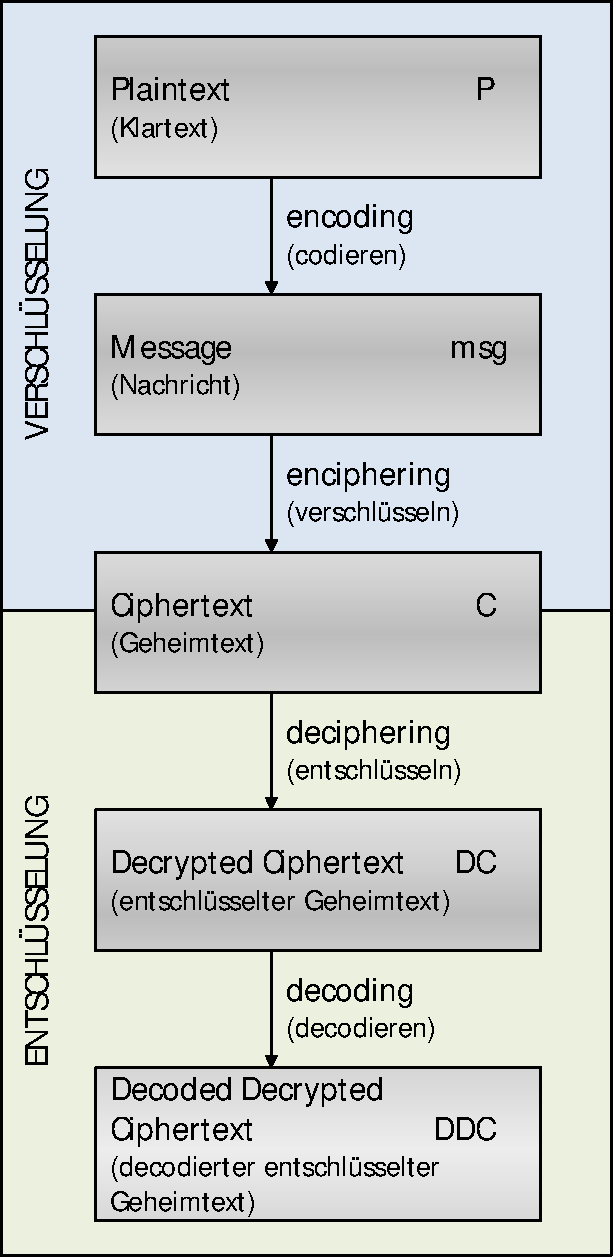
\includegraphics[scale=0.5]{figures/encryption-decryption-de}
\caption{Namenskonventionen in den Sage-Programmbeispielen zu Verschl�sselungsverfahren} 
\label{XXX}
\end{center}
\end{figure}



% ---------------------------------------------------------------------------
\newpage
\subsection{Transpositions-Chiffren}

Tranpositions-Chiffren sind implementiert in der Sage-Klasse
\begin{center}
\verb!sage.crypto.classical.TranspositionCryptosystem!
\end{center}
Bevor man mit einer Sage Transpositions-Chiffre arbeiten kann, muss man sie
konstruieren: Dazu legt man das Alphabet fest, das sie Symbole (Zeichen) enth�lt,
aus denen Klartext und Geheimtext bestehen k�nnen. 
Typischerweise besteht das Alphabet aus den normalen lateinischen Gro�buchstaben.
Dieses Alphabet legt man mit der folgenden Funktion fest
\begin{center}
\verb!sage.monoids.string_monoid.AlphabeticStrings!
\end{center}
Danach muss man die Blockl�nge der Permutation festlegen, d.h. die
L�nge des Zeilenvektors der einfachen Spaltentransposition.
Dieser Zeilenvektor ist der Schl�ssel, mit dem die Buchstaben des
Klartextes permutiert werden.

Im folgenden ersten Beispiel der Transpositions-Chiffren ist die 
Blockl�nge 14, und der Schl�ssel ist so gebaut, dass jeder Buchstabe
im Klartext um zwei Zeichen nach rechts geshiftet wird (und wrap-around
am Ende des Blocks). Das ist der Verschl�sselungsvorgang.
Der Entschl�sselungsvorgang besteht im Shiften jedes Zeichens des
Geheimtextes um $14 - 2 = 12$ Zeichen nach links.

\begin{sagecode}
\begin{Verbatim}%
[fontsize=\footnotesize,fontshape=tt]
sage: # transposition cipher using a block length of 14
sage: T = TranspositionCryptosystem(AlphabeticStrings(), 14)
sage: # given plaintext
sage: P   = "a b c d e f g h i j k l m n"
sage: # encryption key
sage: key = [3, 4, 5, 6, 7, 8, 9, 10, 11, 12, 13, 14, 1, 2]
sage:
sage: # encode plaintext (get rid of non-alphabet chars, convert lower-case to upper-case)
sage: msg = T.encoding(P)
sage: # encrypt plaintext by shifting to the left by 2 letters (do it in two steps)
sage: E   = T(key)
sage: C   = E(msg); C
CDEFGHIJKLMNAB
sage:
sage: # decrypt ciphertext by shifting to the left by 12 letters
sage: keyInv = [13, 14, 1, 2, 3, 4, 5, 6, 7, 8, 9, 10, 11, 12]
sage: D   = T(keyInv)
sage: D(C)
ABCDEFGHIJKLMN
sage:
sage: # Representation of key and inverse key as permutations
sage: E
(1,3,5,7,9,11,13)(2,4,6,8,10,12,14)
sage: D
(1,13,11,9,7,5,3)(2,14,12,10,8,6,4)
\end{Verbatim}
\caption{Einfache Transposition durch Shiften (die Schl�ssel sind explizit gegeben)}
\end{sagecode}

\newpage
Das zweite Beispiel der Transpositions-Chiffren ist ebenfalls eine einfache
shiftende Spaltentransposition. Aber hier ist der Programmcode ein wenig mehr
automatisiert: Die Schl�ssel werden anhand des Shift-Wertes generiert.

\begin{sagecode}
\begin{Verbatim}%
[fontsize=\footnotesize,fontshape=tt]
sage: # transposition cipher using a block length of 14, code more variable
sage: keylen = 14
sage: shift = 2
sage: A = AlphabeticStrings()
sage: T = TranspositionCryptosystem(A, keylen)
sage:
sage: # construct the plaintext string from the first 14 letters of the alphabet plus blanks
sage: # plaintext   = "A B C D E F G H I J K L M N"
sage: A.gens()
(A, B, C, D, E, F, G, H, I, J, K, L, M, N, O, P, Q, R, S, T, U, V, W, X, Y, Z)
sage: P=''
sage: for i in range(keylen): P=P + " " + str(A.gen(i))
....:
sage: P
' A B C D E F G H I J K L M N'
sage:
sage: # encryption key
sage: # key = [3, 4, 5, 6, 7, 8, 9, 10, 11, 12, 13, 14, 1, 2]
sage: key = [(i+shift).mod(keylen) + 1 for i in range(keylen)]; key
[3, 4, 5, 6, 7, 8, 9, 10, 11, 12, 13, 14, 1, 2]
sage:
sage: # encode plaintext (get rid of non-alphabet chars)
sage: msg = T.encoding(P)
sage: # encrypt plaintext by shifting to the left by 2 letters (do it in one step)
sage: C   = T.enciphering(key, msg); C
CDEFGHIJKLMNAB
sage:
sage: # decrypt ciphertext by shifting to the left by 12 letters
sage: # keyInv = [13, 14, 1, 2, 3, 4, 5, 6, 7, 8, 9, 10, 11, 12]
sage: shiftInv=keylen-shift;
sage: keyInv = [(i+shiftInv).mod(keylen) + 1 for i in range(keylen)]; keyInv
[13, 14, 1, 2, 3, 4, 5, 6, 7, 8, 9, 10, 11, 12]
sage: DC   = T.enciphering(keyInv, C); DC
ABCDEFGHIJKLMN
sage:
sage: # decryption using the "deciphering method with key" instead of "enciphering with keyInv" 
sage: # using the deciphering method requires to change the type of the variable key
sage: DC  = T.deciphering(T(key).key(), C); DC
ABCDEFGHIJKLMN
sage:
sage: # representation of key and inverse key as permutations
sage: T(key)
(1,3,5,7,9,11,13)(2,4,6,8,10,12,14)
sage: T(key).key()
(1,3,5,7,9,11,13)(2,4,6,8,10,12,14)
sage: T(keyInv)
(1,13,11,9,7,5,3)(2,14,12,10,8,6,4)
\end{Verbatim}
\caption{Einfache Transposition durch Shiften (die Schl�ssel werden mit "range" konstruiert)}
\end{sagecode}

\newpage
Im dritten Beispiel der Transpositions-Chiffren wird eine beliebige Permutation
als Schl�ssel f�r die Ver- und Entschl�sselun gew�hlt, um die Zeichen in jedem Block
zu verw�rfeln (Blockl�nge = Anzahl Spalten in der einfachen Spaltentransposition).
Ist die Blockl�nge $n$, dann ist der Schl�ssel eine Permutation �ber $n$ Zeichen.
Das folgende Beispiel nutzt die Methode \verb!random_key()! der Klasse
\verb!TranspositionCryptosystem!.  Jeder Aufruf von \verb!random_key()! erzeugt
einen anderen Schl�ssel. Deshalb werden bei Ihrem Aufruf voraussichtlich andere
Ergebnisse (Schl�ssel und Geheimtext) auftreten.

\begin{sagecode}
\begin{Verbatim}%
[fontsize=\footnotesize,fontshape=tt]
sage: # Remark: Enciphering here requires, that the length of msg is a multiple of keylen
sage: keylen = 14   # length of key
sage: A = AlphabeticStrings()
sage: T = TranspositionCryptosystem(A, keylen); T
Transposition cryptosystem on Free alphabetic string monoid on A-Z of block length 14
sage:
sage: P = "a b c d e f g h i j k l m n o p q r s t u v w x y z a b"
sage: key = T.random_key(); key
(1,2,3,13,6,5,4,12,7)(11,14)
sage: msg = T.encoding(P); msg
ABCDEFGHIJKLMNOPQRSTUVWXYZAB
sage: C   = T.enciphering(key, msg); C
BCMLDEAHIJNGFKPQAZRSOVWXBUTY
sage: # decryption using the "deciphering method with key" instead of "enciphering with keyInv" 
ssage: DC  = T.deciphering(key, C); DC
ABCDEFGHIJKLMNOPQRSTUVWXYZAB
sage:
sage: # Just another way of decryption: Using "enciphering" with the inverse key
sage: keyInv = T.inverse_key(key); keyInv
(1,7,12,4,5,6,13,3,2)(11,14)
sage: DC     = T.enciphering(keyInv, C); DC
ABCDEFGHIJKLMNOPQRSTUVWXYZAB
sage:
sage: # Test correctness of decryption
sage: msg == DC
True
\end{Verbatim}
\caption{Einfache Spalten-Transposition mit zuf�llig erzeugtem (Permutations-)Schl�ssel}
\end{sagecode}


\newpage
Das vierte Beispiel der Transpositions-Chiffren gibt zus�tzlich die Gr��e des Schl�sselraums
einer einfachen Spaltentransposition aus.

\begin{sagecode}
\begin{Verbatim}%
[fontsize=\footnotesize,fontshape=tt]
sage: keylen = 14   # length of key
sage: A = AlphabeticStrings()
sage: T = TranspositionCryptosystem(A, keylen); T
Transposition cryptosystem on Free alphabetic string monoid on A-Z of block length 14
sage: T.key_space()
Symmetric group of order 14! as a permutation group
sage: # Remark: The key space is not quite correct as also permutations shorter than keylen are counted.
sage:
sage: P = "a b c d e f g h i j k l m n o p q r s t u v w x y z a b"
sage: key = T.random_key(); key
(1,2,7)(3,9)(4,5,10,12,8,13,11)(6,14)
sage: msg = T.encoding(P); msg
ABCDEFGHIJKLMNOPQRSTUVWXYZAB
sage:
sage: # enciphering in one and in two steps
sage: C   = T.enciphering(key, msg); C
BGIEJNAMCLDHKFPUWSXBOAQZRVYT
sage:
sage: enc = T(key); enc.key()
(1,2,7)(3,9)(4,5,10,12,8,13,11)(6,14)
sage: C = enc(msg); C
BGIEJNAMCLDHKFPUWSXBOAQZRVYT
sage:
sage: # deciphering
sage: DC  = T.deciphering(key, C); DC
ABCDEFGHIJKLMNOPQRSTUVWXYZAB
\end{Verbatim}
\caption{Einfache Spalten-Transposition (mit Ausgabe der Gr��e des Schl�sselraumes)}
\end{sagecode}



% ---------------------------------------------------------------------------
\newpage
\subsection{Substitutions-Chiffren}

Substitutions-Verschl�sselungen sind in Sage in der folgenden Klasse implementiert
\begin{center}
\verb!sage.crypto.classical.SubstitutionCryptosystem!
\end{center}

\noindent Das folgende Programmbeispiel l�sst Sage eine Substitutions-Chiffre mit
zuf�lligem Schl�ssel erstellen. Den zuf�lligen Schl�ssel kann man mit der Methode
\verb!random_key()! der Klasse \texttt{SubstitutionCrypto\-system} erzeugen.
Unterschiedliche Schl�ssel erzeugen eine unterschiedliche Substitutions-Chiffre.
Deshalb erh�lt man mit jedem Aufruf von \verb!random_key()! voraussichtlich
ein anderes Ergebnis.

\begin{sagecode}
\begin{Verbatim}%
[fontsize=\footnotesize,fontshape=tt]
sage: # plaintext/ciphertext alphabet
sage: A   = AlphabeticStrings()
sage: S   = SubstitutionCryptosystem(A)
sage:
sage: P   = "Substitute this with something else better."
sage: key = S.random_key(); key
INZDHFUXJPATQOYLKSWGVECMRB
sage:
sage: # method encoding can be called from A or from T
sage: msg = A.encoding(P); msg
SUBSTITUTETHISWITHSOMETHINGELSEBETTER
sage: C   = S.enciphering(key, msg); C
WVNWGJGVGHGXJWCJGXWYQHGXJOUHTWHNHGGHS
sage:
sage: #### We now decrypt the ciphertext to recover our plaintext.
sage:
sage: DC  = S.deciphering(key, C); DC
SUBSTITUTETHISWITHSOMETHINGELSEBETTER
sage: msg == DC
True
\end{Verbatim}
\caption{Monoalphabetische Substitution mit zuf�llig erzeugtem Schl�ssel}
\end{sagecode}



% ---------------------------------------------------------------------------
\newpage
\subsection{Caesar-Chiffre}

Das folgende Programmbeispiel erzeugt eine Caesar-Chiffre.

\begin{sagecode}
\begin{Verbatim}%
[fontsize=\footnotesize,fontshape=tt]
sage: # plaintext/ciphertext alphabet
sage: A = AlphabeticStrings()
sage: P = "Shift the alphabet three positions to the right."
sage:
sage: # construct Caesar cipher
sage: S = SubstitutionCryptosystem(A)
sage: key = A([3, 4, 5, 6, 7, 8, 9, 10, 11, 12, 13, 14, 15, 16, 17, 18, 19, \
....:          20, 21, 22, 23, 24, 25, 0, 1, 2])
sage:
sage: # encrypt message
sage: msg     = A.encoding(P); msg
SHIFTTHEALPHABETTHREEPOSITIONSTOTHERIGHT
sage: encrypt = S(key); encrypt
DEFGHIJKLMNOPQRSTUVWXYZABC
sage: C       = encrypt(msg); C
VKLIWWKHDOSKDEHWWKUHHSRVLWLRQVWRWKHULJKW
sage:
sage: #### Next, we recover the plaintext.
sage:
sage: # decrypt message
sage: keyInv = A([23, 24, 25, 0, 1, 2, 3, 4, 5, 6, 7, 8, 9, 10, 11, 12, 13, \
....:             14, 15, 16, 17, 18, 19, 20, 21, 22])
sage: decrypt = S(keyInv); decrypt
XYZABCDEFGHIJKLMNOPQRSTUVW
sage: DC      = decrypt(C); DC
SHIFTTHEALPHABETTHREEPOSITIONSTOTHERIGHT
sage: msg == DC
True
\end{Verbatim}
\caption{Caesar (Substitution durch Shiften des Alphabets; Schl�ssel explizit gegeben; Schritt-f�r-Schritt-Ansatz)}
\end{sagecode}


\newpage
Das zweite Caesar-Beispiel macht dasselbe, aber der Programmcode ist variabler.

\begin{sagecode}
\begin{Verbatim}%
[fontsize=\footnotesize,fontshape=tt]
sage: # plaintext/ciphertext alphabet
sage: A = AlphabeticStrings()
sage: keylen = len(A.gens()); keylen
26
sage: shift  = 3
sage: P = "Shift the alphabet three positions to the right."
sage:
sage: # construct Caesar cipher
sage: S = SubstitutionCryptosystem(A)
sage: S
Substitution cryptosystem on Free alphabetic string monoid on A-Z
sage: # key = A([3, 4, 5, 6, 7, 8, 9, 10, 11, 12, 13, 14, 15, 16, 17, 18, 19, \
sage: #          20, 21, 22, 23, 24, 25, 0, 1, 2])
sage: key = [(i+shift).mod(keylen) for i in range(keylen)];
sage: key = A(key); key
DEFGHIJKLMNOPQRSTUVWXYZABC
sage: len(key)
26
sage:
sage: # encrypt message
sage: msg     = A.encoding(P); msg
SHIFTTHEALPHABETTHREEPOSITIONSTOTHERIGHT
sage: C       = S.enciphering(key, msg); C
VKLIWWKHDOSKDEHWWKUHHSRVLWLRQVWRWKHULJKW
sage:
sage: #### Next, we recover the plaintext.
sage:
sage: # decrypt message
sage: # keyInv = A([23, 24, 25, 0, 1, 2, 3, 4, 5, 6, 7, 8, 9, 10, 11, 12, 13, \
sage: #             14, 15, 16, 17, 18, 19, 20, 21, 22])
sage: shiftInv=keylen-shift;
sage: keyInv = [(i+shiftInv).mod(keylen) for i in range(keylen)];
sage: keyInv = A(keyInv); keyInv
XYZABCDEFGHIJKLMNOPQRSTUVW
sage: DC     = S.enciphering(keyInv, C); DC
SHIFTTHEALPHABETTHREEPOSITIONSTOTHERIGHT
sage:
sage: # Just another way of decryption: Using "deciphering" with the key
sage: DC     = S.deciphering(key, C); DC
SHIFTTHEALPHABETTHREEPOSITIONSTOTHERIGHT
sage:
sage: msg == DC
True
\end{Verbatim}
\caption{Caesar (Substitution durch Shiften des Alphabets; Substitutions-Schl�ssel werden berechnet)}
\end{sagecode}



% ---------------------------------------------------------------------------
\newpage
\subsection{Substitutions-Chiffre mit Symbolen}

Im folgenden Sage-Programmbeispiel sind die Alphabetzeichen aus dem Bin�rsystem.
Eine monoalphabetische Substitution �ber einem Bin�ralphabet bietet nur wenig
Sicherheit: Weil das Klartext-/Geheintext-Alphabet nur aus den 2 Elementen 
0 and 1 besteht, gibt es nur zwei m�gliche Schl�ssel: (0 1) and (1 0).
Anmerkung: In jedem Schl�ssel einer Substitutions-Chiffre m�ssen alle
Alphabetzeihen genau einmal auftreten.

\begin{sagecode}
\begin{Verbatim}%
[fontsize=\footnotesize,fontshape=tt]
sage: # the plaintext/ciphertext alphabet
sage: A = BinaryStrings()
sage: # substitution cipher over the alphabet A; no keylen argument possible
sage: S = SubstitutionCryptosystem(A); S
Substitution cryptosystem on Free binary string monoid
sage: # to have a substitute for each symbol, key has always the length of the alphabet
sage: key = S.random_key(); key
10
sage: len(key)
2
sage: P = "Working with binary numbers."
sage: # encryption
sage: msg = A.encoding(P); msg
01010111011011110111001001101011011010010110111001100111001000000111011101101\
00101110100011010000010000001100010011010010110111001100001011100100111100100\
1000000110111001110101011011010110001001100101011100100111001100101110
sage: C   = S.enciphering(key, msg); C
10101000100100001000110110010100100101101001000110011000110111111000100010010\
11010001011100101111101111110011101100101101001000110011110100011011000011011\
0111111001000110001010100100101001110110011010100011011000110011010001
sage: # decryption
sage: DC  = S.deciphering(key, C); DC
01010111011011110111001001101011011010010110111001100111001000000111011101101\
00101110100011010000010000001100010011010010110111001100001011100100111100100\
1000000110111001110101011011010110001001100101011100100111001100101110
sage: msg == DC
True
\end{Verbatim}
\caption{Monoalphabetische Substitution �ber dem Bin�r-Alphabet}
\end{sagecode}



\newpage
Das zweite Beispiel einer monoalphabetischen Substitution mit Symbolen benutzt
ein gr��eres Alphabet f�r den Klartext-/Geheimtext-Zeichenraum als das erste Beispiel.
Hier wird nun das hexadezimale Zahlensystem als Substitutions-Alphabet verwendet.

\begin{sagecode}
\begin{Verbatim}%
[fontsize=\footnotesize,fontshape=tt]
sage: A = HexadecimalStrings()
sage: S = SubstitutionCryptosystem(A)
sage: key = S.random_key(); key
2b56a4e701c98df3
sage: len(key)
16
sage: # Number of possible keys
sage: factorial(len(key))
20922789888000
sage: P   = "Working with a larger alphabet."
sage:
sage: msg = A.encoding(P); msg
576f726b696e6720776974682061206c617267657220616c7068616265742e
sage: C   = S.enciphering(key, msg); C
47e375e9e1efe75277e17ae052eb52e8eb75e7e47552ebe872e0ebe5e47a5f
sage: DC  = S.deciphering(key, C); DC
576f726b696e6720776974682061206c617267657220616c7068616265742e
sage: msg == DC
True
sage:
sage: # Conversion hex back to ASCII:
sage: # - AlphabeticStrings() and HexadecimalStrings() don't have according methods.
sage: # - So we used Python:
sage: #   - repr(DC) converts the StringMonoidElement DC to a string
sage: #     still containing hex symbols;
sage: #   - binascii.a2b_hex converts this hex string to an ascii string.
sage: import binascii
sage: DDC = binascii.a2b_hex(repr(DC)); DDC
'Working with a larger alphabet.'
sage:
sage: P == DDC
True
\end{Verbatim}
\caption{Monoalphabetische Substitution �ber dem Hexadezimal-Alphabet (Dekodieren in Python)}
\end{sagecode}



% ---------------------------------------------------------------------------
\newpage
\subsection{Vigen{\`e}re-Verschl�sselung}

Die Vigen{\`e}re-Verschl�sselung ist in der folgenden Sage-Klasse implementiert
\begin{center}
\verb!sage.crypto.classical.VigenereCryptosystem!
\end{center}

\noindent Als Klartext-/Geheimtext-Zeichenraum kann man die lateinischen
Gro�buchstaben, das Bin�rsystem, das Oktalsystem oder Hexadezimalsystem w�hlen.
Hier ist ein Beispiel, das mit der Klasse \verb!AlphabeticStrings! die Gro�bucgstaben
nutzt.

\begin{sagecode}
\begin{Verbatim}%
[fontsize=\footnotesize,fontshape=tt]
sage: # construct Vigenere cipher
sage: keylen = 14
sage: A = AlphabeticStrings()
sage: V = VigenereCryptosystem(A, keylen); V
Vigenere cryptosystem on Free alphabetic string monoid on A-Z of period 14
sage:
sage: # alternative: given key: key = A('ABCDEFGHIJKLMN'); key
sage: key = V.random_key(); key
WSSSEEGVVAARUD
sage: len(key)
14
sage:
sage: # encoding
sage: P = "The Vigenere cipher is polyalphabetic."
sage: len(P)
38
sage: msg = V.encoding(P); msg     # alternative: msg = A.encoding(P); msg
THEVIGENERECIPHERISPOLYALPHABETIC
sage:
sage: # encryption [2 alternative ways (in two steps or in one): both work]
sage: # encrypt = V(key); encrypt
sage: # C = encrypt(msg); C
sage: C   = V.enciphering(key, msg); C
PZWNMKKIZRETCSDWJAWTUGTALGBDXWLAG
sage:
sage: # decryption
sage: DC  = V.deciphering(key, C); DC
THEVIGENERECIPHERISPOLYALPHABETIC
sage: msg == DC
True
\end{Verbatim}
\caption{Vigen{\`e}re-Verschl�sselung}
\end{sagecode}




% ---------------------------------------------------------------------------
\newpage
\subsection{Hill-Verschl�sselung}

Das Hill~\cite{Hill1929,Hill1931}- oder Matrix-Verschl�sselung genannte
Verfahren ist mathematisch anspruchsvoller als die Verfahren in den bisherigen
Programmbeispielen dieses Kapitels. Der Ver-/Entschl�sselungs-Schl�ssel dieses
Verfahrens ist eine invertierbare quadratische Matrix, und der Klar-/Geheimtext
wird ebenfalls als Matrix verarbeitet. Die Ver- und Entschl�sselungsprozesse
nutzen Matrizen-Operationen. Die Hill-Verschl�sselung ist implementiert in der
folgenden Sage-Klasse
\begin{center}
\verb!sage.crypto.classical.HillCryptosystem!
\end{center}

Im folgenden Beispiel besteht der Klar-/Geheimtext-Zeichenraum wieder aus
den Gro�buchstaben des lateinischen Alphabets. Im Hill-Verfahren wird
jedem Alphabet-Zeichen eine eindeutige nat�rliche Zahl modulo 26 zugewiesen.

\begin{sagecode}
\begin{Verbatim}%
[fontsize=\footnotesize,fontshape=tt]
sage: # construct a Hill cipher
sage: keylen = 19    # keylen = 3  # Alternative key length with non-random small key
sage: A = AlphabeticStrings()
sage: H = HillCryptosystem(A, keylen); H
Hill cryptosystem on Free alphabetic string monoid on A-Z of block length 19
sage:
sage: # To create key non-randomly, HKS is necessary [even H.key_space() is not enough].
sage: # HKS = H.key_space()
sage: # key = HKS([[1,0,1],[0,1,1],[2,2,3]]); key
sage:
sage: # Random key creation
sage: key = H.random_key(); key
[10  7  5  2  0  6 10 23 15  7 17 19 18  2  9 12  0 10 11]
[23  1  1 10  4  9 21  1 25 22 19  8 17 22 15  8 12 25 22]
[ 4 12 16 15  1 12 24  5  9 13  5 15  8 21 23 24 22 20  6]
[ 5 11  6  7  3 12  8  9 21 20  9  4 16 18 10  3  2 23 18]
[ 8 22 14 14 20 13 21 19  3 13  2 11 13 23  9 25 25  6  8]
[24 25  8 24  7 18  3 20  6 11 25  5  6 19  7 24  2  4 10]
[15 25 11  1  4  7 11 24 20  2 18  4  9  8 12 19 24  0 12]
[14  6  2  9 11 20 13  4 10 11  4 23 14 22 14 16  9 12 18]
[12 10 21  5 21 15 16 17 19 20  1  1 15  5  0  2 23  4 14]
[21 15 15 16 15 20  4 10 25  7 15  4  7 12 24  9 19 10  6]
[25 15  2  3 17 23 21 16  8 18 23  4 22 11 15 19  6  0 15]
[14 23  9  3 18 15 10 18  7  5 12 23 11  9 22 21 20  4 14]
[ 3  6  8 13 20 16 11  1 13 10  4 21 25 15 12  3  0 11 18]
[21 25 14  6 11  3 21  0 19 17  5  8  5  4  9  2 23 19 15]
[ 8 11  9 11 20 15  6  1  3 18 18 22 16 17  6  3 15 11  2]
[21 15  5 22  2  9  0  4 22 10  2 10 19 19 17 19  1 21  4]
[ 7 17  9  2 15  5 14  3  6  9 12 12 22 15  8  4 21 14 19]
[19 14 24 19  7  5 22 22 13 14  7 18 17 19 25  2  1 23  6]
[ 2  6 14 22 17  7 23  6 22  7 13 20  0 14 23 17  6  1 12]
sage:
sage: # encoding and encryption
sage: P = "Hill or matrix cipher uses matrix operations."
sage: len(P)
45
sage: # implementation requires: Length of msg is a multiple of matrix dimension (block_length)
sage: msg = H.encoding(P); msg
HILLORMATRIXCIPHERUSESMATRIXOPERATIONS
sage: len(msg)
38
sage:
sage: # encryption
sage: C  = H.enciphering(key, msg); C
CRWCKPRVYXNBRZTNZCTQWFWSDWBCHABGMNEHVP
sage:
sage: # decryption
sage: DC  = H.deciphering(key, C); DC
HILLORMATRIXCIPHERUSESMATRIXOPERATIONS
sage: msg == DC
True
sage:
sage: # alternative decryption using inverse matrix
sage: keyInv = H.inverse_key(key); keyInv
[ 6 23  1 23  3 12 17 22  6 16 22 14 18  3  1 10 21 16 20]
[18 23 15 25 24 23  7  4 10  7 21  7  9  0 13 22  5  5 23]
...
[10 11 12  6 11 17 13  9 19 16 14 24  4  8  5 16 18 20  1]
[19 16 16 21  1 19  7 12  3 18  1 17  7 10 24 21  7 16 11]
sage: DC     = H.enciphering(keyInv, C); DC
HILLORMATRIXCIPHERUSESMATRIXOPERATIONS
\end{Verbatim}
\caption{Hill-Verschl�sselung}
\end{sagecode}







%------------------------------------------------------------------------------
\newpage
\begin{thebibliography}{99999}
\addcontentsline{toc}{section}{Literaturverzeichnis}

\bibitem[ACA2002]{ACA2002} \index{ACA 2002}
   American Cryptogram Association, \\
   {\em Length and Standards for all ACA Ciphers}, \\
   2002.\\
   \href{http://www.cryptogram.org/cdb/aca.info/aca.and.you/chap08.html#}
   {\texttt{http://www.cryptogram.org/cdb/aca.info/aca.and.you/chap08.html\#}}

\bibitem[Bauer1995]{Bauer1995} \index{Bauer 1995}
   Friedrich L. Bauer, \\
   {\em Entzifferte Geheimnisse}, Springer, 1995.

\bibitem[Bauer2000]{Bauer2000} \index{Bauer 2000}
   Friedrich L. Bauer, \\
   {\em Decrypted Secrets}, Springer 1997, 2nd edition 2000.

\bibitem[Crowley2000]{Crowley2000} \index{Crowley 2000}
   Paul Crowley, \\
   {\em Mirdek: A card cipher inspired by "`Solitaire"'}, \\
   2000.\\
   \href{http://www.ciphergoth.org/crypto/mirdek/}
   {\texttt{http://www.ciphergoth.org/crypto/mirdek/}}

\bibitem[DA1999]{DA1999} \index{DA 1999}
   Data encryption page des ThinkQuest Team 27158 f�r ThinkQuest 1999 \\
   (Kein Update seit 1999, keine Suchm�glichkeit), \\
   1999.\\
   \href{http://library.thinkquest.org/27158/}
   {\texttt{http://library.thinkquest.org/27158/}}

\bibitem[Goebel2003]{Goebel2003} \index{Goebel 2003}
   Greg Goebel, \\
   {\em Codes, Ciphers and Codebreaking}, \\
   2003.\\
   \href{http://www.vectorsite.net/ttcode.htm}
   {\texttt{http://www.vectorsite.net/ttcode.htm}}

\bibitem[Hill1929]{Hill1929} \index{Hill 1929}
   Lester S. Hill,\\
   ``Cryptography in an Algebraic Alphabet,''
   \emph{The American Mathematical Monthly}, 36(6):306--312, 1929.

\bibitem[Hill1931]{Hill1931} \index{Hill 1931}
   Lester S. Hill,\\
   ``Concerning Certain Linear Transformation Apparatus of Cryptography,''
   \emph{The American Mathematical Monthly}, 38(3):135--154, 1931.
	
\bibitem[Nichols1996]{Nichols1996} \index{Nichols 1996} 
    Randall K. Nichols, \\
    {\em Classical Cryptography Course, Volume 1 and 2}, \\
    Aegean Park Press 1996; \\
    oder in 12 Lektionen online unter \\
    \href{http://www.fortunecity.com/skyscraper/coding/379/lesson1.htm}
    {\texttt{http://www.fortunecity.com/skyscraper/coding/379/lesson1.htm}}

\bibitem[Savard1999]{Savard1999} \index{Savard 1999}
	John J. G. Savard, \\
	{\em A Cryptographic Compendium}, \\
	1999.\\
	\href{http://www.hypermaths.org/quadibloc/crypto/jscrypt.htm}
	{\texttt{http://www.hypermaths.org/quadibloc/crypto/jscrypt.htm}}
% manchmal schlecht zu erreichen, auch wenn man von seiner Homepage
% http://www.hypermaths.org/quadibloc/main.htm    aus startet.
% http://www.hypermaths.org/quadibloc/crypto/jscrypt.htm
	
\bibitem[Schmeh2004]{Schmeh2004}  \index{Schmeh 2004}
        Klaus Schmeh, \\
        {\em Die Welt der geheimen Zeichen. Die faszinierende Geschichte der Verschl�sselung},\\ 
        W3L Verlag Bochum, 1. Auflage 2004.

\bibitem[Schmeh2007]{Schmeh2007}  \index{Schmeh 2007}
        Klaus Schmeh, \\
        {\em Codeknacker gegen Codemacher. Die faszinierende Geschichte der Verschl�sselung.},\\ 
        W3L Verlag Bochum, 2. Auflage 2007.\\
	Dieses Buch ist das aktuellste unter denen, die sich mit der Geschichte der Kryptographie besch�ftigen. Es enth�lt eine kleine Sammlung gel�ster und ungel�ster Krypto-R�tsel.



\bibitem[Schneier1999]{Schneier1999}
	Bruce Schneier, \\
	{\em The Solitaire Encryption Algorithm}, \\
	version 1.2, 1999.\\
	\href{http://www.schneier.com/solitaire.html}
	{\texttt{http://www.schneier.com/solitaire.html}}

\bibitem[Singh2001]{Singh2001} \index{Singh 2001}
	Simon Singh, \\
	{\em Geheime Botschaften. Die Kunst der Verschl�sselung von der 
        Antike bis in die Zeiten des Internet}, \\
	dtv, 2001.

\bibitem[ThinkQuest1999]{ThinkQuest1999} \index{ThinkQuest 1999}
	ThinkQuest Team 27158, \\
	{\em Data Encryption}, \\
	1999.\\
	\href{http://library.thinkquest.org/27158/}
	{\texttt{http://library.thinkquest.org/27158/} }

	
%xxxxxxxxxxx
%\bibitem[x]{x}  \index{x}
%        x, \\
%        {\em x}, 
%       x x.
%xxxxxxxxxxx

% ddddddddddddddddddddddddddddddddddddddddx

\end{thebibliography}








% Local Variables:
% TeX-master: "../script-de.tex"
% End:


\renewcommand{\CTBChapName}{(Chap Primes)}        % $Id$
%%%%%%%%%%%%%%%%%%%%%%%%%%%%%%%%%%%%%%%%%%%%%%%%%%%%%%%%%%%%%%%%%%%%%%%%%%
%
% C H A P T E R   T H R E E :  P R I M E S
%
%%%%%%%%%%%%%%%%%%%%%%%%%%%%%%%%%%%%%%%%%%%%%%%%%%%%%%%%%%%%%%%%%%%%%%%%%%

\newpage
% \hypertarget{Kapitel_2}{}
\chapter{Prime Numbers}
\label{Label_Kapitel_Primes}
(Bernhard Esslinger, May 1999; Updates Nov. 2000, Dec. 2001, June 2003, May 2005, March 2006, June 2007, Jan. 2010, Dec. 2012)

\begin{ctsquote}
    Progress requires exchange of knowledge.
\caption[Albert Einstein]{Albert Einstein\footnotemark}
\end{ctsquote}
\addtocounter{footnote}{0}\footnotetext{%
  Albert Einstein, German physicist and Nobel Prize winner, 
  Mar 14, 1879 $-$ Apr 14, 1955.
}

% --------------------------------------------------------------------------
\section{What are prime numbers?}
\index{Prime number} \index{Number!prime}
Prime numbers are whole, positive numbers greater than or equal to $2$ that can
only be divided by 1 and themselves. All other natural numbers (composite
numbers) can be formed by multiplying prime numbers.

\noindent The {\em natural} \index{Number!natural} numbers
$\mathbb{N}=\{1, 2, 3, 4,\cdots \}$ thus comprise 
\begin{itemize}
   \item the number $1$ (the unit value)
   \item the primes and
   \item the composite numbers.
\end{itemize}

\noindent Prime numbers are particularly important for three reasons:
\begin{itemize}
  \item In number theory, they are considered to be the basic components of
natural numbers, upon which numerous brilliant mathematical ideas are based.
  \item They are of extreme practical importance in modern
\index{Cryptography!modern} cryptography (public key \index{Cryptography!public key} cryptography). The most common public key procedure, invented at the end of
the 1970's, is \index{RSA} RSA encryption. Only using (large) prime numbers for
particular parameters can you guarantee that an algorithm is secure, both for
the RSA procedure and for even more modern procedures (e.g. elliptic curves).
  \item The search for the largest known prime numbers does not have any
practical usage known to date, but requires the best computers, is an excellent
benchmark (possibility for determining the performance\index{Performance} of computers) and leads
to new calculation methods on many computers \\
(see also: \url{http://www.mersenne.org/prime.htm}).
\end{itemize}
Many people have been fascinated by prime numbers over the past two millennia.
Ambition to make new discoveries about prime numbers has often resulted in
brilliant ideas and conclusions. The following section provides an easily
comprehensible introduction to the basics of prime numbers. We will also
explain what is known about the distribution (density, number of prime numbers
in particular intervals) of prime numbers and how prime number tests work.


% --------------------------------------------------------------------------
\section{Prime numbers in mathematics}\label{primesinmath}

Every whole number has a factor. The number 1 only has one factor,
itself, whereas the number $12$ has the six factors $1, 2, 3, 4,
6, 12$. Many numbers can only be divided by themselves and by $1$.
With respect to multiplication, these are the ``atoms'' in the
area of numbers. Such numbers are called prime numbers.

In mathematics, a slightly different (but equivalent) definition is used.

\begin{definition}\label{def-pz-prime}
A whole number $p \in {\bf N}$ is called prime \index{Number!prime} if
$p > 1$ and $p$ only possesses the trivial factors $\pm 1$ and $\pm p$.
\end{definition}


By definition, the number $1$ is not a prime number. In the following sections,
$p$ will always denote a prime number.

The sequence of prime numbers starts with $$ 2,~ 3,~ 5,~ 7, ~ 11, ~ 13, ~
17, ~ 19, ~ 23, ~ 29, ~ 31, ~ 37, ~ 41, ~ 43, ~ 47, ~ 53, ~ 59, ~ 61,
~ 67, ~ 71, ~ 73, ~ 79, ~ 83, ~ 89, ~ 97, \cdots . $$
The first 100 numbers include precisely 25 prime numbers. After this,
the percentage of primes constantly decreases. Prime numbers can be
factorized in a uniquely {\em trivial} way: 
$$5 = 1 \cdot 5,\quad  17 = 1 \cdot 17, \quad 1013 = 1 \cdot 1013,  \quad
1,296,409 = 1 \cdot 1,296,409.$$
All numbers that have $2$ or more factors not equal 1 are called 
\index{Number!composite} {\em composite} numbers. 
These include $$ 4 = 2 \cdot 2, \quad 6 = 2\cdot 3 $$ as well
as numbers that {\em look like primes}, but are in fact composite:
$$ 91 = 7 \cdot 13, \quad 161=7 \cdot 23, \quad 767 =13 \cdot 59. $$

\begin{theorem}\label{thm-pz-sqr}
Each whole number $m$ greater than $1$ possesses a lowest factor greater than
$1$. This is a prime number $p$. Unless $m$ is a prime number itself, then: $p$
is less than or equal to the square root of $m$.
\end{theorem}

All whole numbers greater than $1$ can be expressed as a product of prime
numbers --- in a unique way. This is the claim of the \textbf{1st fundamental theorem of
number theory} (= fundamental theorem of arithmetic = fundamental building block
of all positive integers).\index{Number theory!fundamental theorem}

\begin{theorem}\label{thm-pz-prod}
Each element $n$ of the natural numbers greater than $1$ can be written as the
product $n = p_1 \cdot p_2 \dots p_m$ of prime numbers. If two such
factorizations $$n =  p_1 \cdot p_2 \cdot \cdots \cdot p_m = p'_1 \cdot p'_2 \cdots
p'_{m'}$$ are given, then they can be reordered such that $\;m = m'\;$ and for
all $i$:  $\;p_i = p'_i$. \\
($p_1, p_2, \dots, p_m$ are called the prime factors of n).
\end{theorem}

In other words: each natural number other than $1$ can be written as a product
of prime numbers in precisely one way, if we ignore the order of the factors.
The factors are therefore unique (the {\em expression as a product of factors}
is unique)! For example, $$ 60 = 2 \cdot 2 \cdot 3 \cdot 5 = 2^2\cdot 3^1 \cdot
5^1. $$
And this --- other than changing the order of the factors --- is the only way in
which the number $60$ can be factorized. If you allow numbers other than primes
as factors, there are several ways of factorizing integers and the \textbf{uniqueness} \hypertarget{uniqueness}{} is
lost: $$ 60 = 1 \cdot 60 = 2 \cdot 30 = 4 \cdot 15 = 5 \cdot 12 =6 \cdot 10 = 2
\cdot 3 \cdot 10 = 2 \cdot 5 \cdot 6 = 3 \cdot 4 \cdot 5 = \cdots . $$

The following section is aimed more at those familiar with mathematical logic:
The 1st fundamental theorem only appears to be obvious \label{remFundTheoOfArithm}. We can construct
numerous other sets of numbers (i.e. other than positive whole numbers greater
than 1), for which numbers in the set cannot be expressed uniquely as a product
of the prime numbers of the set: In the set $M = \{1, 5, 10, 15, 20, \cdots\}$
there is no equivalent to the fundamental theorem under multiplication. The
first five prime numbers of this sequence are $5, 10, 15, 20, 30$ (note: $10$ is
prime, because $5$ is not a factor of $10$ in this set --- the result is not an
element of the given basic set $M$). Because the following applies in $M$: $$
100 = 5 \cdot 20 = 10 \cdot 10 $$ and $5, 10, 20$ are all prime numbers in this
set, the expression as a product of prime factors is not unique here.

% --------------------------------------------------------------------------
\section{How many prime numbers are there?}

For the natural numbers, the primes can be compared to elements in chemistry or
the elementary particles in physics (see \cite[p. 22]{pr:Blum1999}).

Although there are only $92$ natural chemical elements, the number of prime
numbers is unlimited. Even the Greek, \index{Euclid} Euclid%
\footnote{Euclid,
a Greek mathematician of 4th and 3rd century B.C. He worked at the
Egyptian academy of Alexandria and wrote ``The Elements'', the most well 
known systematically textbook of the Greek mathematics.} 
knew this in the third century B.C.
\begin{theorem}[Euclid\footnote{The common usage of the term does not denote Euclid as the inventor of the theorem rather;
the true inventor is merely not as prominent. The theorem has already been distinguished
and proven in Euclid's Elements (Book IX, theorem 20). The phraseology is remarkable due to 
the fact that the word infinite is not used. The text reads as followed
$$
O\acute{\iota}~\pi\varrho\tilde{\omega}\tau o \iota~\grave{\alpha}\varrho\iota\vartheta\mu o\grave{\iota}~
\pi\lambda\varepsilon\acute{\iota}o \upsilon\varsigma~\varepsilon\grave{\iota}\sigma\grave{\iota}~
\pi\alpha\nu\tau\grave{o}\varsigma~\tau o \tilde{\upsilon}~
\pi\varrho o \tau\varepsilon\vartheta\acute{\varepsilon}\nu\tau o \varsigma~
\pi\lambda\acute{\eta}\vartheta\ o \upsilon\varsigma~
\pi\varrho\acute{\omega}\tau\omega\nu~
\grave{\alpha}\varrho\iota\vartheta\mu\tilde{\omega}\nu,
$$
the English translation of which is: the prime numbers are more than 
any previously existing amount of prime numbers.
}]\label{thm-pz-euklid} % Ende der Fu�note
% Fussnote VOR "]" in [Euclid], damit kein Leerraum vor der Fussnotennummer.
% Vorher stand da: ...(Euclid). BLANK Fussnote und das Blank stoerte.
% Nun steht die Fussnote direkt hinter "Euclid" und vor der ")".
% Eigentlich h�tte ich sie gerne direkt hinter "(Euclid)", noch vor dem 
% automatisch gesetzten Punkt. 
The sequence of prime numbers does not discontinue.
Therefore, the quantity of prime numbers is infinite.
\end{theorem}
His proof that there is an infinite number of
primes is still considered to be a brilliant mathematical consideration and
conclusion today (\textbf{proof by contradiction} \index{Proof by contradiction}). 
He assumed that there is only a finite number of primes and therefore a 
largest prime number. Based on this assumption, he drew logical conclusions
until he obtained an obvious contradiction. This meant that something must
be wrong. As there were no mistakes in the chain of conclusions, it could
only be the assumption that was wrong. Therefore, there must be an infinite
number of primes!\\

\hypertarget{euclid}{}
\index{Euclid's proof by contradiction}\index{Proof by contradiction}
% \paragraph*{Euclid's proof by contradiction}
% goes as follows:
\begin{Proof}{according to Euclid (proof by contradiction)\\}
{\bf Assumption:} \quad There is a {\em finite} number of primes. \\*[4pt] {\bf
Conclusion:} \quad Then these can be listed $p_1 < p_2 < p_3 < \dots < p_n$,
where $n$ is the (finite) number of prime numbers. $p_n$ is therefore the
largest prime. Euclid now looks at the number $a = p_1 \cdot p_2 \cdots p_n +1$.
This number cannot be a prime number because it is not included in our list of
primes. It must therefore be divisible by a prime, i.e. there is a natural
number $i$ between $1$ and $n$, such that $p_i$ divides the number $a$. Of
course, $p_i$ also divides the product $a-1 = p_1 \cdot p_2 \cdots p_n$, because
$p_i$ is a factor of $a-1$. Since $ p_i $ divides the numbers $ a $ and $ a-1 $,
it also divides the difference of these numbers. Thus: $p_i$ divides  $a - (a-1)
= 1$. $p_i$ must therefore divide $1$, which is impossible. \\*[4pt] {\bf
Contradiction:} \quad Our assumption was false.

Thus there is an {\em infinite} number of primes
(Cross-reference: \hyperlink{primhfk}{overview} under \ref{s:primhfk} of 
the number of prime numbers in various intervals).
\end{Proof} 

\par \vskip + 10pt

Here we should perhaps mention yet another fact which is initially somewhat surprising. 
Namely, in the prime numbers sequence $p_1, p_2, \cdots,$ gaps between prime numbers can have
an individually determined length $n$. It is undeniable that under the $n$
succession of natural numbers
$$(n+1)!+2,\cdots, (n+1)!+(n+1),
$$
none of them is a prime number since in order, the numbers $2,3,\cdots,(n+1)$  
are comprised respectively as real divisors. 
($n!$ means the product of the first $n$ natural numbers therefore 
$ n!= n*(n-1)*\cdots *2*1$).


% --------------------------------------------------------------------------
% --------------------------------------------------------------------------
\vskip + 20pt
\section{The search for extremely large primes}
\label{search_for_very_big_primes}   % chap. 3.4

The largest prime numbers known today have several millions digits, 
which is too big for us to imagine. The number of elementary particles in
the universe is estimated to be ``only'' a $80$-digit number 
\hyperlink{grosord}{(See: overview under \ref{s:grosord}
of various orders of magnitude / dimensions)}.


% --------------------------------------------------------------------------
\hypertarget{RecordPrimes}{}
\subsection{The 20+ largest known primes (as of July 2012)}  % Eyecatcher_neue-Mersenne
\label{RecordPrimes}
\index{Prime number!records}

The following table contains the biggest, currently known primes and
a description of its particular number type\footnote{%
An up-to-date version can be found in the internet at
     \url{http://primes.utm.edu/largest.html}
and at
     \url{http://primes.utm.edu/mersenne/index.html}.
}:

\index{Mersenne!number!generalized}
\index{Fermat!number!generalized} 

\begin{table} % don't use [h] (error if table has >24 lines)
\begin{center}
\begin{tabular}{|c|cccc|}
\hline    % Eyecatcher_neue-Mersenne
	& {\bf Definition} & {\bf Decimal Digits} & {\bf When} & {\bf Description} \\
\hline
	1  & $2^{43,112,609}-1$ & 12,978,189 & 2008 & Mersenne, 47th known \\
	2  & $2^{42,643,801}-1$ & 12,837,064 & 2009 & Mersenne, 46th known \\
	3  & $2^{37,156,667}-1$ & 11,185,272 & 2008 & Mersenne, 45th known \\

	4  & $2^{32,582,657}-1$ &  9,808,358 & 2006 & Mersenne, 44th known \\
	5  & $2^{30,402,457}-1$ &  9,152,052 & 2005 & Mersenne, 43rd known \\
	6  & $2^{25,964,951}-1$ &  7,816,230 & 2005 & Mersenne, 42nd known \\
	7  & $2^{24,036,583}-1$ &  7,235,733 & 2004 & Mersenne, M-41 \\
	8  & $2^{20,996,011}-1$ &  6,320,430 & 2003 & Mersenne, M-40 \\
	9  & $2^{13,466,917}-1$ &  4,053,946 & 2001 & Mersenne, M-39 \\
	10 & $19,249 \cdot 2^{13,018,586}+1$ & 3,918,990 & 2007 & Generalized Mersenne\footnotemark \\
	11 & $27,653 \cdot 2^{9,167,433}+1$ & 2,759,677 & 2005 & Generalized Mersenne \\



	12 & $28,433 \cdot 2^{7,830,457}+1$ & 2,357,207 & 2004 & Generalized Mersenne \\

	13  & $2^{ 6,972,593}-1$ & 2,098,960 & 1999 & Mersenne, M-38 \\
	14  & $5,359 \cdot 2^{5,054,502}+1$ & 1,521,561 & 2003 & Generalized Mersenne \\

	15  & $4,847 \cdot 2^{3,321,063}+1$ & 999,744 & 2005 & Generalized Mersenne \\
	16  & $3 \cdot 2^{3,136,255}-1$ & 944,108 & 2007 & Generalized Mersenne \\

	17  & $2^{ 3,021,377}-1$ &   909,526 & 1998 & Mersenne, M-37 \\
	18  & $2^{ 2,976,221}-1$ &   895,932 & 1997 & Mersenne, M-36 \\

	19  & $222,361 \cdot 2^{2,854,840}+1$ & 859,398 & 2006 & Generalized Mersenne \\

	20 & $1,372,930^{131,072}+1$ &   804,474 & 2003 & Generalized Fermat\footnotemark \\

	21  & $1,361,244^{131,072}+1$ &   803,988 & 2004 & Generalized Fermat \\
	22  & $1,176,694^{131,072}+1$ &   795,695 & 2003 & Generalized Fermat \\

	23  & $342,673 \cdot 2^{2,639,439}-1$ & 794,556 & 2007 & Generalized Mersenne \\

\hline
\end{tabular}
\caption{The 20+ largest known primes and its particular number types
         (as of July 2012)}    % Eyecatcher_neue-Mersenne
\label{L_n_Largest_Known-Primes}
\end{center}
\end{table} 
\addtocounter{footnote}{-1}
\footnotetext{\index{Number!Sierpinski}\index{Seventeen or Bust SoB}%
This number was found within the distributed computing project
``Seventeen or Bust'' (SoB) (\url{http://www.seventeenorbust.com})
% {\href{http://www.mersenne.org} {\tt http://www.mersenne.org}}
at March 26, 2007. While the well known \hyperlink{GIMPS-project}{GIMPS project} (chapter~\ref{zahlentyp_mersenne}) searches for bigger and bigger of the infinitely many primes, there is a chance, that the SoB project could have been completed its task sometime.

The SoB project tries to prove computationally, that the number $k = 78,557$ is
the smallest Sierpinski number (John Selfridge proved in 1962, that $78,557$ is a Sierpinski number).

The famous Polish mathematician Waclaw Sierpinski (1882 to 1969) proved in
1960, that there exist infinitely many odd integers k, which fulfill the
following property: For all Sierpinski numbers k it is true: All numbers $N = k \cdot 2^{n}+1$ are composite for all integers $n>=1$ (Sierpinski's Composite Number Theorem, \url{http://mathworld.wolfram.com/SierpinskisCompositeNumberTheorem.html}).

When the project started in 2002 there have been 17 possible candidates $< 78557$ (this is the reason for the project's name ``Seventeen or Bust''). It is sufficient to find one single counter-example, to exclude a candidate k, which means to find a single $n>=1$, where $N = k \cdot 2^{n}+1$ is prime. So it is only a byproduct of this task that this also generates new monster primes.
} 
\addtocounter{footnote}{1}
\footnotetext{%
Generalized Fermat number: $ 1,372,930^{131,072} + 1 = 1,372,930^{(2^{17})}+1 $
\index{Fermat!number!generalized}  } 
%be_2005: Erzwingen, dass die Abb. noch in diesem Kapitel !

The largest known prime is a Mersenne prime, found by the
\hyperlink{GIMPS-project}{GIMPS project}(chapter~\ref{zahlentyp_mersenne}).

Within the largest known primes there are also numbers of the type
\hyperlink{generalizedMersennenumbers}{generalized Mersenne number}
(chapter~\ref{generalized-mersenne-no1})
and 
\hyperlink{generalizedFermatprimes}{generalized Fermat numbers}
(chapter~\ref{generalized-fermat}).


% --------------------------------------------------------------------------
\hypertarget{MersenneNumbers01}{}
\subsection{Special number types -- Mersenne numbers and Mersenne primes} 
\label{zahlentyp_mersenne}
\index{Mersenne!number}

Almost all known huge prime numbers are special candidates, called
\index{Mersenne, Marin} {\em Mersenne numbers}\footnote{%
Marin Mersenne, French priest and mathematician, Sep 08, 1588 $-$ Sep 01, 1648.
\index{Mersenne, Marin}
}
of the form $2^p -1,$ where $p$ is
a prime. Not all Mersenne numbers are prime:

$$
\begin{array}{cl}
2^2 - 1 = 3 & \Rightarrow {\rm prime} \\
2^3 - 1 = 7 & \Rightarrow {\rm prime} \\
2^5 - 1 = 31    & \Rightarrow {\rm prime} \\
2^7 - 1 = 127    & \Rightarrow {\rm prime} \\
2^{11} - 1 = 2,047 = 23 \cdot 89    & \Rightarrow  {\rm NOT~prime} !
\end{array}
$$

\index{Number!Mersenne}\index{Mersenne!number}
\index{Mersenne!theorem} 

Even Mersenne knew that not all Mersenne numbers
are prime (see exponent $p = 11$). 
A prime Mersenne number \index{Mersenne!prime number} is called
Mersenne prime number.  \\
However, he is to be thanked for the interesting conclusion that a number 
of the form $2^n-1$ cannot be a prime number if $n$ is a composite number:

\begin{theorem}[Mersenne]\label{thm-pz-mersenne} 
  If $2^n - 1$ is a prime number, then $n$ is also a prime number.
\end{theorem}

\begin{Proof}{}
The theorem of Mersenne can be proved by contradiction%
\index{Proof by contradiction}.  We therefore assume that
there exists a composite natural number $ n $ (with real factorization)  
$ n=n_1 \cdot n_2 $
, with the property that $ 2^n -1 $ is a prime number.

From \begin{eqnarray*} (x^r-1)((x^r)^{s-1} + (x^r)^{s-2} + \cdots + x^r +1) & =
&  ((x^r)^s + (x^r)^{s-1} + (x^r)^{s-2} + \cdots + x^r) \\ &  & -((x^r)^{s-1} +
(x^r)^{s-2} + \cdots + x^r +1)  \\ & = & (x^r)^s -1 = x^{rs } -1,
\end{eqnarray*} we conclude \[ 2^{n_1 n_2} - 1 = (2^{n_1} -1)((2^{n_1})^{n_2 -1}
+ (2^{n_1})^{n_2 -2} + \cdots + 2^{n_1} + 1). \]
Because $ 2^n - 1 $ is a prime number, one of the above two factors on the
right-hand side must be equal to 1. This is the case if and only if $ n_1 =1 $
or $ n_2 =1$. But this contradicts our assumption. Therefore the assumption is
false. This means that there exists no composite number $ n, $ such that $ 2^n -
1 $ is a prime.
\end{Proof} 

\vskip + 5pt
\hypertarget{Mer-nums-not-always-prim}{}
Unfortunately this theorem only applies in one direction (the inverse 
statement does not apply, no equivalence): that means that there exist 
prime exponent for which the Mersenne number is {\bf not} prime (see the 
above example $2^{11}-1, $ where $11$ is prime, but $2^{11}-1$ not).

Mersenne claimed that $2^{67}-1$ is a prime number. There is also a mathematical
history behind this claim: it first took over 200 years before 
\index{Lucas, Edouard} Edouard Lucas (1842-1891) proved that this number 
is composite.
However, he argued indirectly and did not name any of the factors. In 1903,
Cole\index{Cole, Frank Nelson}\footnote{%
Frank Nelson Cole, American mathematician, Sep. 20, 1861 $-$ May 26, 1926.}
showed which factors make up this composite number: 
$$ 2^{67} -1
=147, 573, 952, 589, 676, 412, 927 = 193, 707, 721 \cdot 761, 838, 257, 287. $$
He admitted to having worked 20 years on the factorization 
\index{Factorization} (expression as a product of prime factors)\footnote{%
  Using CT1\index{CrypTool 1} you can factorize numbers in the 
  following way: menu {\bf Indiv. Procedures \textbackslash{} RSA Cryptosystem 
  \textbackslash{} Factorization of a Number}. \\
  CT1 can factorize with the quadratic sieve (QS) on a single PC in a reasonable
  time numbers no longer than 250 bit.
  Numbers bigger than 1024 bits are currently not accepted by CT1. \\
  With CT2 you can use both the QS and the GNFS (general number field sieve),
  and CT2 can distribute the calculations on several computers.\\
  The current factorization records are listed in chapter \ref{nt:NoteFactorization}.
  \index{Factorization!factoring records}
}
of this 21-digit decimal number!

Due to the fact that the exponents of the Mersenne numbers
\index{Mersenne!number} do not use all
natural numbers, but only the primes, the {\em experimental space} is limited
considerably. The currently known Mersenne prime numbers 
\index{Mersenne!prime number} have the exponents\footnote{%
Landon Curt Noll\index{Noll, Landon Curt} lists all known Mersenne primes
including its date of discovery and its value as number and as word:
      \url{http://www.isthe.com/chongo/tech/math/prime/mersenne.html} \\
Also see:
      \url{http://www.utm.edu/}.
                             } 
$$
\begin{array}{c}
2; ~ 3; ~ 5; ~ 7; ~ 13; ~ 17; ~ 19; ~ 31; ~ 61; ~ 89; ~ 107; ~ 127;
~ 521; ~ 607; ~ 1,279; ~ 2,203; ~ 2,281; ~ 3,217;\\
4,253; ~ 4,423; ~ 9,689; ~ 9,941, ~ 11,213; ~ 19,937; ~ 21,701; ~ 23,207; ~ 44,497; ~
86,243; ~ 110,503; \\
132,049; ~ 216,091; ~ 756,839; ~ 859,433; ~ 1,257,787; ~ 1,398,269; ~ 2,976,221; ~ 3,021,377;\\
6,972,593; ~ 13,466,917; ~ 20,996,011; ~ 24,036,583; ~ 25,964,951; ~ 30,402,457;\\
32,582,657; ~ 37,156,667; ~ 42,643,801, ~ 43,112,609.
% be_2005_UPDATEN_if-new-mersenne-prime-appears          ~ xxx,xxx,xxx.
\end{array}
$$
Thus    % Eyecatcher_neue-Mersenne
$47$            % be_2005_UPDATEN_if-new-mersenne-prime-appears
Mersenne prime numbers are currently known%
\index{Prime number!Mersenne}\index{Mersenne!prime number}. 

The $19$th number with the exponent $4,253$ was the first with at least $1,000$ digits in  decimal system
(the mathematician Samual \index{Yates, Samual} Yates coined the expression {\em
titanic} \index{Prime number!titanic} prime for this; it was discovered by
Hurwitz in 1961); the $27$th number with the exponent $44,497$ was the first
with at least $10,000$ digits in the decimal system (Yates coined the expression
\index{Prime number!gigantic}  {\em gigantic} prime for this. These names are
now long outdated).


\vskip +10 pt
For the first 41            % be_2005_UPDATEN_if-new-mersenne-prime-appears    % Eyecatcher_neue-Mersenne
Mersenne prime numbers we know that this list is complete.
The exponents until the 47th     % be_2005_UPDATEN_if-new-mersenne-prime-appear    % Eyecatcher_neue-Mersennes
Mersenne prime number have not yet been checked completely.\footnote{%
The current status of the check can be found at:
      \url{http://www.mersenne.org/status.htm}.\\
Hints, how the primality of a number can be checked, are in chapter
\ref{primality_tests}, prime number tests\index{Prime number!test}. }


% be_2005_UPDATEN_if-new-mersenne-prime-appears    % Eyecatcher_neue-Mersenne
Right now (July 2012) all prime exponents smaller than $ 24,212,801 $ have been
tested and double-checked\footnote{%
See home page of the GIMPS project:
      \url{http://www.mersenne.org/report_milestones}.
                                  }:
So we can
be certain, that this is really the 41th Mersenne prime number and that
there are no smaller undiscovered Mersenne primes (it is common usage to use
the notation M-nn not until it is proven, that the nn-th known Mersenne prime
is really the nn-th Mersenne prime). Here are some examples in more detail:


\vskip +15 pt
\paragraph*{M-37 -- January 1998}\index{Mersenne!prime number!M-37}\mbox{}

The 37th Mersenne prime, $$ 2^{3,021,377} - 1 $$
was found in January 1998 and has 909,526
digits in the decimal system, which corresponds to 33 pages in the newspaper!


\vskip +25 pt
\paragraph*{M-38 -- June 1999}\index{Mersenne!prime number!M-38}\mbox{}

The 38th Mersenne prime, called M-38, $$ 2^{6,972,593} - 1 $$
was discovered in June 1999 and has $2,098,960$ digits in the decimal system
(that corresponds to around 77 pages in the newspaper).


\vskip +25 pt
\hypertarget{M-39}{}
\paragraph*{M-39 -- December 2001}%
\index{Mersenne!prime number!M-39}\mbox{}

The 39th Mersenne prime, called M-39, $$2^{13,466,917}-1,$$ was
published at December 6, 2001 -- more exactly, the verification of this number,
found at November 14, 2001 by the Canadian student Michael Cameron, was
successfully completed. 
This number has about 4 million decimal digits (exactly 4,053,946 digits).
Trying only to print this number 
$$(924947738006701322247758 \cdots 1130073855470256259071)$$
would require around 200 pages in the Financial Times.

%\vskip +15 pt
%\paragraph*{Mxxxxxxxxxx -- June 2003 -- M-40 ?}%
%\index{Mersenne!prime number!M-40}\mbox{}
%\vskip +10 pt

%This number was discovered as 40th Mersenne prime (and already called M-40,
%despite it has not been proven yet, whether no further Mersenne prime
%numbers between M-39 und Mxxxxxxxxx do indeed exist), $$2^{xx,xxx,xxx}-1,$$
%at June xx, 2003 -- more exactly, the verification of this number,
%found at June 02, 2003 by xxxxxxxxxx, was
%successfully completed. 
%The initiator and project leader George Woltman only announces a found
%Mersenne number, after another double-check confirms that it is prime.
%This number has about xx million decimal digits
%(exactly xx,xxx,xxx digits).




\vskip +25 pt
\paragraph*{GIMPS}\index{GIMPS}\mbox{}
\hypertarget{GIMPS-project}{}

The GIMPS project (Great Internet Mersenne Prime Search)\index{GIMPS} was
founded in 1996 by George Woltman\index{Woltman, George} to search for new
largest Mersenne primes ({\url{http://www.mersenne.org}}).
Further explanations about this number type can be found under
\hyperlink{MersenneNumbers02}{Mersenne numbers} and 
\hyperlink{MersenneNumbers01}{Mersenne primes}.

Right now the GIMPS project has discovered 13
   % be_2005_UPDATEN_if-new-mersenne-prime-appears    % Eyecatcher_neue-Mersenne
largest Mersenne primes so far, including the largest known prime number at all. 

Table \ref{Primes_GIMPS-Primes_table-reference} contains these Mersenne record
primes.\footnote{%
An up-to-date version can be found in the internet at
     \url{http://www.mersenne.org/history.htm}.
}$^,$\footnote{%
Always, when a new record is published in the respective forums the same
and often ironic discussions start: Does this kind of research have a deeper
sense? Can this result be applied for anything useful?
The answer is, that we don't know it yet. In fundamental research one
cannot see at once whether and how it brings mankind forward.
%But this is the normal case with basic research, that one cannot see at once, 
}

   % be_2005_UPDATEN_if-new-mersenne-prime-appears    % Eyecatcher_neue-Mersenne
\begin{table}[ht]
\begin{center}
\begin{tabular}{|cccc|}
\hline
	{\bf Definition} & {\bf Decimal Digits} & {\bf When} & {\bf Who} \\
\hline

	$2^{43,112,609}-1$ & 12,978,189 & August 23, 2008 & Edson Smith  \\
	$2^{42,643,801}-1$ & 12,837,064 & April 12, 2009 & Odd Magnar Strindmo \\
	$2^{37,156,667}-1$ & 11,185,272 & September 6, 2008 & Hans-Michael Elvenich \\

	$2^{32,582,657}-1$ &  9,808,358 & September 4, 2006 & Curtis Cooper/Steven Boone \\
	$2^{30,402,457}-1$ &  9,152,052 & December 15, 2005 & Curtis Cooper/Steven Boone \\
	$2^{25,964,951}-1$ &  7,816,230 & February 18, 2005 & Martin Nowak     \\
	$2^{24,036,583}-1$ &  7,235,733 & May 15, 2004      & Josh Findley     \\
	$2^{20,996,011}-1$ &  6,320,430 & November 17, 2003 & Michael Shafer   \\
	$2^{13,466,917}-1$ &  4,053,946 & November 14, 2001 & Michael Cameron  \\
	$2^{ 6,972,593}-1$ &  2,098,960 & June 1, 1999      & Nayan Hajratwala \\
	$2^{ 3,021,377}-1$ &    909,526 & January 27, 1998  & Roland Clarkson  \\
	$2^{ 2,976,221}-1$ &    895,932 & August 24, 1997   & Gordon Spence    \\
	$2^{ 1,398,269}-1$ &    420,921 & November 1996     & Joel Armengaud   \\

\hline
\end{tabular}
   % be_2005_UPDATEN_if-new-mersenne-prime-appears    % Eyecatcher_neue-Mersenne
\caption{The largest primes found by the GIMPS project (as of July 2012)}
\label{Primes_GIMPS-Primes_table-reference}
\end{center}
\end{table} 

%be_2005: Erzwingen, dass die Abb. noch in diesem Kapitel !

Richard Crandall\index{Crandall, Richard} discovered the advanced 
transform algorithm used by the GIMPS program. George Woltman implemented
Crandall's algorithm in machine language, thereby producing a prime-search 
program of unprecedented efficiency,
and that work led to the successful GIMPS project.

On June 1st, 2003 a possible Mersenne prime was reported to the GIMPS server, 
which was checked afterwards as usual, before it was to be published. 
Unfortunately mid June the initiator and GIMPS project leader George Woltman
had to tell, that two independent verification runs proved the number 
was composite. This was the first false positive report of a client in 7 years.

Now more than 130,000 volunteers, amateurs and experts, participate in the 
GIMPS project. They connect their computers into the so called ``primenet'', 
organized by the company entropia.






% --------------------------------------------------------------------------
\vskip +25 pt
\subsection{Challenge of the Electronic Frontier Foundation (EFF)}\index{EFF}
This search is also spurred on by a competition started by the non-profit
organization EFF (Electronic Frontier Foundation) using the means of an 
unknown donor. The participants are rewarded with a total of 500,000 USD if
they find the longest prime number. In promoting this project, the unknown
donor is not looking for the quickest computer, but rather wants to draw 
people's attention to the opportunities offered by {\em cooperative networking} \\
{\url{http://www.eff.org/awards/coop}}

The discoverer of M-38 received 50,000 USD from the EFF for discovering 
the first prime with more than 1 million decimal digits. 

% be_2005_UPDATEN_if-new-mersenne-prime-appears
For the next prize of 100,000 USD offered by EFF for a proven prime with more
than 10 million decimal digits, Edson Smith qualified, who found the number
$ 2^{43,112,609}-1 $ within the GIMPS project.
%{\url{http://www.octocad.demon.co.uk/mersenne/prime.htm }}.

According to the EFF rules for their prizes they offer in the next stage
150,000 USD for a proven prime with more than 100 million decimal digits.

Edouard Lucas\index{Lucas, Edouard} (1842-1891) held the record for the
longest prime number for over 70 years by proving that $2^{127}-1$ is prime.
No new record is likely to last that long.


% --------------------------------------------------------------------------
\section[Prime number tests]{Prime number tests\footnotemark}
\footnotetext{%
    \index{NT, Learning Tool for Number Theory}%
    \index{Educational tool NT}%
    With the educational tool for number theory {\bf NT} you can apply the
    tests of Fermat and of Miller-Rabin:
    See NT learning units 3.2 and 3.3, pages 3-11/11.\\
    NT can be called in CT1\index{CrypTool 1} via the menu path
    {\bf Indiv. Procedures \textbackslash{} Number Theory Interactive
    \textbackslash{} Learning Tool for Number Theory}.
    See also appendix \ref{s:appendix-Learn-NT}.\\
    CT2\index{CrypTool 2} contains a visualisation of these methods within
    the tutorial ``{\bf World of Primes}''.
}
\label{primality_tests}   % chap. 3.5
\index{Prime number!test}

In order to implement secure encryption procedures we need extremely large prime
numbers (in the region of $2^{2,048}$, i.e. numbers with $600$ digits in the
decimal system!).

If we look for the prime factors in order to decide whether a number is prime,
then the search takes too long, if even the smallest prime factor is enormous.
Factorizing numbers using systematic computational
division or using the \hyperlink{SieveEratosthenes01}{sieve of Eratosthenes} 
\index{Eratosthenes!sieve} is only feasible using current computers for
numbers with up to around $20$ digits in the decimal system.
The biggest number factorized into its 2 almost equal prime factors 
has 232 digits 
(see \hyperlink{RSA-768-chap3}{RSA-768} in chapter \ref{nt:NoteFactorization}).
% be_2005_UPDATEN_if-new-factorization-record-appears

However, if we know something about the {\em construction} of the number in
question, there are extremely highly developed procedures that are much quicker.
These procedures can determine the primality attribute of a number, but they
cannot determine the prime factors of a number, if it is compound.

\hypertarget{FermatNumbers01}{}\label{FermatNumbers01}%
In the 17th century, Fermat\footnote{%
Pierre de Fermat, French mathematician, Aug 17, 1601 -- Jan 12, 1665.
\index{Fermat, Pierre}
}
\index{Fermat, Pierre} wrote to Mersenne \index{Mersenne, Marin} that he 
presumed that all numbers of the form 
$$ f(n) = 2^{2^n} + 1 $$ 
are prime for all whole numbers $ n \geq 0$ 
(\hyperlink{FermatNumbers02}{see below}, chapter~\ref{L-FermatNumbers02}).
\index{Number!Fermat}\index{Fermat!number}

As early as in the 19th century, it was discovered that the $29$-digit number $$
f(7) = 2^{2^7} + 1 $$ is not prime. However, it was not until 1970 that
Morrison/Billhart managed to factorize it.
\label{F7Morrison}
\begin{eqnarray*}
f(7) & = & 340,282,366,920,938,463,463,374,607,431,768,211,457 \\
& = & 59, 649, 589, 127, 497, 217 \cdot  5,704,689,200,685,129,054,721
\end{eqnarray*}


\vspace{12pt}
Despite Fermat was wrong with this supposition, he is the originator of
an important theorem in this area: Many rapid prime number tests are 
based on the (little) Fermat theorem put forward by Fermat in 1640
(\hyperlink{KleinerSatzFermat-chap3}{see chapter 
\ref{Label_KleinerSatzFermat-chap3}}).

\hypertarget{KleinerSatzFermat-chap2}{}
\index{Fermat!little theorem}
\begin{theorem}[``little'' Fermat]\label{thm-pz-fermat1}
Let $p$ be a prime number and $a$ be any whole number, then for all $a$ $$a^p
\equiv a \; {\rm mod} \; p.$$
This could also be formulated as follows: \\ Let $p$ be a prime number and $a$
be any whole number that is not a multiple of $p$ (also $a \not\equiv 0 \; {\rm
mod} \; p$), then $a^{p-1} \equiv 1 \; {\rm mod} \; p$.
\end{theorem}

If you are not used to calculate with remainders (modulo), please simply
accept the theorem or first read \hyperlink{Chapter_ElementaryNT}
{chapter \ref{Chapter_ElementaryNT} ``Introduction to Elementary Number Theory with 
Examples''}.  What is important here is that this sentence implies that if
this equation is not met for any whole number $a$, then $p$ is not a prime! The
tests (e.g.\ for the first formulation) can easily be performed using the {\em
test basis} $a = 2$.

This gives us a criterion for non-prime numbers, i.e. a negative test, but no
proof that a number $a$ is prime. Unfortunately Fermat's theorem does not apply
--- otherwise we would have a simple proof of the prime number property (or to
put it in other words, we would have a simple prime number criterion).

\vskip +25 pt
\paragraph*{Pseudo prime numbers}%
\index{Prime number!pseudo prime} \index{Number!pseudo prime}%
\hypertarget{HT-Pseudoprimenumber01}{}\label{L-Pseudoprimenumber01}%
\mbox{}
\vskip +10 pt
Numbers n that have the property $$ 2^n \equiv 2 \;{\rm mod}\; n $$
but are not prime are called {\em pseudo prime numbers}
(i.e. the exponent is not a prime). 
The first pseudo prime number is $$ 341 = 11 \cdot 31 .$$


\vskip +25 pt
\paragraph*{Carmichael numbers}%
\index{Number!Carmichael}%
\hypertarget{HT-Carmichael-number01}{}\label{L-Carmichael-number01}%
\mbox{}
\vskip +10 pt
There are pseudo prime numbers n that pass the Fermat test 
$$ a^{n-1} \equiv 1 \;{\rm mod}\; n $$
with all bases a which are relatively prime to n [$ gcd (a,n) = 1 $],
despite these numbers n are not prime: These numbers are called
{\em Carmichael numbers}.
The first of these is $$ 561 = 3 \cdot 11 \cdot 17 .$$

Sample: The number to be tested is 561. Because $ 561 = 3 \cdot 11 \cdot 17 $
it is: \\
The test condition $ a^{560} \;{\rm mod}\; 561 = 1 $ is satisfied 
for $a = 2, 4, 5, 7, \cdots $,\\
but not for $a = 3, 6, 9, 11, 12, 15, 17, 18, 21, 22, \cdots $.\\ 
This means the test condition must not be satisfied for multiples of the
prime factors 3, 11 or 17.\\
The test applied for $a=3$ results in: $ 3^{560} \;{\rm mod}\; 561 = 375 $.\\
The test applied for $a=5$ results in: $ 5^{560} \;{\rm mod}\; 561 = 1 $.


\vskip +25 pt
\paragraph*{Strong pseudo prime numbers}%
\index{Prime number!strong pseudo prime}\index{Number!strong pseudo prime}%
\hypertarget{HT-Strongpseudoprimenumber01}{}\label{L-Strongpseudoprimenumber01}%
\mbox{}
\vskip +10 pt
A stronger test is provided by\index{Miller, Gary L.}\index{Rabin, Michael O.}
Miller/Rabin\footnote{
In 1976 an efficient probabilistic primality test was published by Prof. Rabin, based on a number theoretic result of Prof. Miller from the year before. \\
Prof. Miller worked at the Carnegie-Mellon University, School of Computer
Science. Prof. Rabin, born in 1931, worked at the Harvard and Hebrew University.
}%
: It is only passed by so-called {\em strong pseudo prime numbers}. 
Again, there are strong pseudo prime numbers that are not primes, but this is
much less often the case than for (simple) pseudo prime numbers or for 
Carmichael numbers. The smallest strong pseudo prime number base $2$ is 
$$ 15,841 = 7 \cdot 31 \cdot 73. $$
If you test all 4 bases, $2, 3, 5$ and $7$, you will find only one strong
pseudo prime number up to $25 \cdot 10^9$, i.e. a number that passes the 
test and yet is not a prime number.

More extensive mathematics behind the Rabin test delivers the probability that
the number examined is prime (such probabilities are currently around $10^{-
60}$).

Detailed descriptions of tests for finding out whether a number is prime
can be found on Web sites such as:
\vspace{-10pt}
\begin{itemize}
  \item[] \url{http://www.utm.edu/research/primes/mersenne.shtml} \\
          \url{http://www.utm.edu/research/primes/prove/index.html}
\end{itemize}


% --------------------------------------------------------------------------
\vskip +30 pt
% caused a warning black rectangle:
%\section{Special number types and the search for a formula for primes}
\section{Special types of numbers and the search for a formula for primes}
\label{spezialzahlentypen}
\index{Prime number!formula}
There are currently no useful, open (i.e. not recursive) formulae known that
only deliver prime numbers (recursive means that in order to calculate the
function the same function is used with a smaller variable). Mathematicians
would be happy if they could find a formula that leaves gaps (i.e. does not
deliver all prime numbers) but does not deliver any composite (non-prime)
numbers.

Ideally, we would like, for the number $n$, to immediately be able to 
obtain the $n$-th prime number, i.e. for $f(8) = 19\,$ or for  $f(52) = 239$.

Ideas for this can be found at
\vspace{-10pt}
\begin{itemize}
  \item[] {\url{http://www.utm.edu/research/primes/notes/faq/p_n.html}}.
\end{itemize}


Cross-reference:  \hyperlink{ntePrimzahl}{the table under \ref{s:ntePrimzahl}}
contains the precise values for the $n$th prime numbers for selected $ n.$
\\

For ``prime number formulae'' usually very special types of numbers are used.
The following enumeration contains the most common ideas for 
``prime number formulae'', and what our current knowledge is about
very big elements of the number series: Is their primality proven?
If their are compound numbers could their prime factors be determined?


% --------------------------------------------------------------------------
\vskip +10 pt
\hypertarget{MersenneNumbers02}{}
\subsection{Mersenne numbers \texorpdfstring{$f(n) = 2^n - 1$  \quad for $ n $ prime}
	   			      {f(n) = 2\^{}n - 1 for n prime}}
    \index{Prime number!Mersenne} \index{Mersenne!prime number}
    As shown \hyperlink{MersenneNumbers01}{above}, this formula seems
    to deliver relatively large prime numbers but - as for $n=11$ 
    [$f(n)=2,047$] - it is repeatedly the case that the result even with
    prime exponents is \hyperlink{Mer-nums-not-always-prim}{not} prime.\\
    Today, all the Mersenne primes having less than around 4,000,000 digits
    are known (\hyperlink{M-39}{M-39}\index{Mersenne!prime number!M-39}):
\vspace{-10pt}
\begin{itemize}
  \item[] {\url{http://perso.wanadoo.fr/yves.gallot/primes/index.html}}
\end{itemize}      % be_2005_UPDATEN_if-new-mersenne-prime-appears

% --------------------------------------------------------------------------
\vskip +10 pt
\subsection
   [Generalized Mersenne numbers \texorpdfstring{$f(k,n) = k \cdot 2^n \pm 1$}{f(k,n) = k .... 2\^{}n +- 1} / Proth numbers]
   {Generalized Mersenne numbers
   $f(k,n) = k \cdot 2^n \pm 1 $  for $ n $ prime and $ k $ small prime
    / Proth numbers\footnotemark}
    \footnotetext{%
       Their names come from the French farmer Fran�ois Proth (1852-1879).
       More famous as the Proth primes is the related Sierpinski 
       problem\index{Number!Sierpinski}: Find all numbers k, so that
       $k*2^n+1$ is composite for all n > 0.
       See table \ref{L_n_Largest_Known-Primes}.
    }
   \label{generalized-mersenne-no1}

   This first generalization of the Mersenne
   numbers\index{Mersenne!number!generalized}
   creates the so called Proth numbers\index{Number!Proth}.
   There are (for small $k$) extremely quick prime number tests
   (see \cite{pr:Knuth1981}). This can be performed in practice using software
   such as the Proths software from Yves Gallot\index{Gallot, Yves}:
\vspace{-10pt}
\begin{itemize}
  \item[] {\url{http://www.prothsearch.net/index.html}}.
\end{itemize}


% --------------------------------------------------------------------------
\vskip +10 pt
\hypertarget{generalizedMersennenumbers}{}
\subsection
   [Generalized Mersenne numbers \texorpdfstring{$ f(b,n) = b^n \pm 1 $}{f(b,n) = b\^{}n +- 1} / 
    Cunningham project]
   {Generalized Mersenne numbers 
   $ f(b,n) = b^n \pm 1 $ / The Cunningham project}

   This is another possible generalisation of the Mersenne 
   numbers\index{Mersenne!number!generalized}.
   The \index{Cunningham project} \textbf{Cunningham project} determines
   the factors of all composite numbers that are formed as follows:
   $$ f(b,n) = b^n \pm 1  \quad {\rm for~} b = 2, 3, 5, 6, 7, 10, 11, 12 $$
   ($b$ is not equal to multiples of bases already used, such as $4, 8, 9$).

   Details of this can be found at:
\vspace{-10pt}
\begin{itemize}
  \item[] {\url{http://www.cerias.purdue.edu/homes/ssw/cun}}
\end{itemize}


% --------------------------------------------------------------------------
\vskip +10 pt
\hypertarget{FermatNumbers02}{}
\subsection[Fermat numbers \texorpdfstring{$f(n) = 2^{2^n} + 1$}{f(n) = 2\^{}2\^{}n + 1}]
              {Fermat numbers\footnotemark~$f(n) = 2^{2^n} + 1$} 
    \footnotetext{%
       The Fermat prime numbers play a role in circle division.
       As proven by Gauss\index{Gauss, Carl Friedrich} a regular $p$-edge
       can only be constructed with the use of a pair of compasses and a 
       ruler, when $p$ is a Fermat prime number.
    }
    \label{L-FermatNumbers02}
    \index{Prime number!Fermat} \index{Fermat!prime number}       
    As mentioned \hyperlink{FermatNumbers01}{above} in 
    chapter~\ref{FermatNumbers01}, Fermat wrote to Mersenne regarding 
    his assumption, that all numbers of this type are primes.
    This assumption was disproved by Euler (1732). The prime $641$ divides
    $f(5)$.\footnote{%
    Surprisingly this number can easily be found by using Fermat's theorem (see e.g.\ \cite[p. 176]{pr:Scheid1994})
    } 
%    Surprisingly he would have been able obtain a positive result using
%    the negative prime number test for $n=5$ based on his small theorem.
$$
\begin{array}{lll}
f(0) = 2^{2^0} + 1  = 2^1 + 1 & = 3 &   \mapsto {\rm ~prime}  \\
f(1) = 2^{2^1} + 1  = 2^2 + 1 & = 5 &   \mapsto {\rm ~prime}  \\
f(2) = 2^{2^2} + 1  = 2^4 + 1 & = 17 &  \mapsto {\rm ~prime}  \\
f(3) = 2^{2^3} + 1  = 2^8 + 1 & = 257 & \mapsto {\rm ~prime}  \\
f(4) = 2^{2^4} + 1  = 2^{16} + 1 &  = \mbox{65,537} &  \mapsto {\rm ~prime}  \\
f(5) = 2^{2^5} + 1  = 2^{32} + 1 &  = \mbox{4,294,967,297} = 641 \cdot \mbox{6,700,417} &  \mapsto {\rm ~NOT~prime} ! \\
f(6) = 2^{2^6} + 1  = 2^{64} + 1 &  = \mbox{18,446,744,073,709,551,617} \\
                                 &  = \mbox{274,177} \cdot \mbox{67,280,421,310,721} & \mapsto {\rm ~NOT~prime} !\\
f(7) = 2^{2^7} + 1  = 2^{128} + 1 & = \mbox{(see page~\pageref{F7Morrison})}  
																 & \mapsto {\rm ~NOT~prime} !

\end{array} 
$$

    Within the project ``Distributed Search for Fermat Number Dividers''
    offered by Leonid Durman there is also progress in finding new monster
    primes: 
\vspace{-10pt}
\begin{itemize}
  \item[] {\url{http://www.fermatsearch.org/}}\\
       This website links to other web pages in Russian, Italian and German.
\end{itemize}
    The discovered factors can be compound integers or primes.
     
    On February 22, 2003 John Cosgrave discovered 
    \begin{itemize} 
     \item the largest composite Fermat number to date and
     \item the largest prime non-simple Mersenne number so far with
           645,817 decimal digits.
    \end{itemize}
    
    The Fermat number
    $$ f(2,145,351) = 2^{(2^{2,145,351})} + 1 $$ 
    is divisible by the prime
    $$ p = 3*2^{2,145,353} + 1 $$ \\
    At that time this prime p was the largest known prime generalized Mersenne 
    number\index{Mersenne!number!generalized} and the
    5th largest known prime number at all. 

    This work was done using NewPGen from Paul Jobling's, PRP from 
    George Woltman's, Proth from Yves Gallot's programs\index{Gallot, Yves} and
    also the Proth-Gallot group at St. Patrick's College, Dublin.

    More details are in
    \vspace{-10pt}
    \begin{itemize}
      \item[] \url{http://www.fermatsearch.org/history/cosgrave_record.htm/}
    \end{itemize}

%    ({\url{http://perso.wanadoo.fr/yves.gallot/primes/index.html}}).
% M.E. ist die Zahl auf seiner Webseite zu gro�, da M-39 "nur" 4 Mio. Stellen hat !
%    Heute kennt man alle Fermatschen Primzahlen mit bis zu 2.000.000.000 ??? 
%    Dezimalstellen. \\



% --------------------------------------------------------------------------
\vskip +10 pt
\hypertarget{generalizedFermatprimes}{}
\subsection[Generalized Fermat numbers \texorpdfstring{$f(b,n) = b^{2^n} + 1$}{f(b,n) = b\^{}2\^{}n + 1}]
              {Generalized Fermat numbers\footnotemark~$f(b,n) = b^{2^n} + 1$}
    \footnotetext{%
      The base of this power is no longer restricted to 2.
      Even more generic would be:  $f(b,c,n) = b^{c^n} \pm 1$
    }
\label{generalized-fermat}
\index{Fermat!number!generalized} 
    Generalized Fermat numbers are more numerous than Mersenne numbers of a
    equal size and many of them are waiting to be discovered to fill the
    big gaps between the Mersenne primes already found or still undiscovered.
    Progress in number theory made it possible that numbers, where the
    representation is not limited to the base 2, can be tested at almost
    the same speed than a Mersenne number.
    
    Yves Gallot\index{Gallot, Yves} wrote the program Proth.exe to investigate
    generalized Fermat numbers.
    
    Using this program at February 16, 2003 Michael Angel discovered the
    largest of them till then with 628,808 digits, which at that time became
    the 5th largest known prime number:
    $$ b^{2^{17}} + 1  =  62,722^{131,072} + 1. $$ 

    More details are in
    \vspace{-10pt}
    \begin{itemize}
      \item[] \url{http://primes.utm.edu/top20/page.php?id=12}
    \end{itemize}



% --------------------------------------------------------------------------
\vskip +10 pt
\subsection{Carmichael numbers}\index{Number!Carmichael}
As mentioned \hyperlink{HT-Carmichael-number01}{above} in
chapter~\ref{L-Carmichael-number01} not all Carmichael numbers are prime.


% --------------------------------------------------------------------------
\vskip +10 pt
\subsection{Pseudo prime numbers}
\index{Prime number!pseudo prime}\index{Number!pseudo prime}
See \hyperlink{HT-Pseudoprimenumber01}{above} in
chapter~\ref{L-Pseudoprimenumber01}.


% --------------------------------------------------------------------------
\vskip +10 pt
\subsection{Strong pseudo prime numbers}
\index{Prime number!strong pseudo prime}\index{Number!strong pseudo prime}
See \hyperlink{HT-Strongpseudoprimenumber01}{above} in
chapter~\ref{L-Strongpseudoprimenumber01}.



% --------------------------------------------------------------------------
\vskip +10 pt
\subsection
    [Idea based on Euclid's proof \texorpdfstring{$p_1 \cdot p_2 \cdots p_n +1$}{p\_1 ... p\_2 ... p\_n +1}]
    {Idea based on Euclid's proof $p_1 \cdot p_2 \cdots p_n +1$}
This idea is based on \hyperlink{euclid}{Euclid's proof} that there are
infinite many prime numbers.
$$
\begin{array}{lll}
2{\cdot}3 +1 &      = 7 &          \mapsto {\rm ~prime} \\
2{\cdot}3{\cdot}5 +1 &      = 31    &      \mapsto {\rm ~prime} \\
2{\cdot}3{\cdot}5{\cdot}7 +1 &      = 211   &      \mapsto {\rm ~prime} \\
2{\cdot}3{\cdots}11 +1 &        = 2,311  &      \mapsto {\rm ~prime} \\
2\cdot3 \cdots 13 +1 &  = 59 \cdot 509 &    \mapsto {\rm ~NOT~prime} ! \\
2\cdot3 \cdots 17 +1 &  = 19 \cdot 97 \cdot 277 &   \mapsto {\rm ~NOT~prime} !
\\
\end{array}
$$


% --------------------------------------------------------------------------
\vskip +10 pt
\subsection{As above but \texorpdfstring{$-1$ except $+1$: $p_1 \cdot p_2 \cdots p_n -1$}
                                        {-1 except +1: p\_1 ... p\_2 ... p\_n -1}}
$$
\begin{array}{lll}
2\cdot 3 -1     &   = 5 &   \mapsto {\rm ~prime} \\
2\cdot 3 \cdot  5  -1   &   = 29 &  \mapsto {\rm ~prime} \\
2\cdot 3 \cdots 7  -1   &   = 11 \cdot 19 & \mapsto {\rm ~NOT~prime} ! \\
2\cdot 3 \cdots 11 -1   &   = 2,309 &    \mapsto {\rm ~prime} \\
2\cdot 3 \cdots 13 -1   &   = 30,029 &    \mapsto {\rm ~prime} \\
2\cdot 3 \cdots 17 -1    &  = 61 \cdot 8,369 &   \mapsto {\rm ~NOT~prime!}
\end{array} 
$$


% --------------------------------------------------------------------------
\vskip +10 pt
\subsection[Euclidean numbers \texorpdfstring{$e_n = e_0 \cdot e_1 \cdots e_{n-1} + 1$}
                                             {e\_n = e\_0 ... e\_1 e\_n-1 + 1}]
              {Euclidean numbers $e_n = e_0 \cdot e_1 \cdots e_{n-1} + 1$
	       with $ n \geq 1 $ and $ e_0 := 1 $}
%	       with $n$ greater than or equal to $1$ and $e_0 := 1$}
    \index{Euclidean number}
    $e_{n-1}$ is not the $(n-1)$th prime number, but the number 
    previously found here.
    Unfortunately this formula is not open but recursive.
    The sequence starts with 

$$
\begin{array}{lll}
e_1 = 1 + 1 &   = 2 &   \mapsto {\rm ~prime} \\
e_2 = e_1 + 1   &   = 3 &   \mapsto {\rm ~prime} \\
e_3 = e_1 \cdot e_2 + 1 &   = 7 &   \mapsto {\rm ~prime} \\
e_4 = e_1 \cdot e_2 \cdot e_3 + 1 & = 43 &  \mapsto {\rm ~prime} \\
e_5 = e_1 \cdot e_2 \cdots e_4 + 1 &    = 13 \cdot 139 &    \mapsto {\rm
~NOT~prime} ! \\
e_6 = e_1 \cdot e_2 \cdots e_5 + 1 &    = 3,263,443 &   \mapsto {\rm ~prime} \\
e_7 = e_1 \cdot e_2 \cdots e_6 + 1 &    = 547 \cdot 607 \cdot 1,033 \cdot 31,051
& \mapsto {\rm ~NOT~prime} ! \\
e_8 = e_1 \cdot e_2 \cdots e_7 + 1 &    = 29,881\cdot 67,003 \cdot 9,119,521
\cdot 6,212,157,481 & \mapsto {\rm ~NOT~prime} !
\end{array} 
$$

\noindent Also $e_9, \cdots, e_{17}$ are composite, which means that this formula is not
particularly useful. 

\begin{remark}{:}\\
However, what is special about these numbers is that any pair of 
them does not have a common factor other than $1$\footnote{%
This can easily be shown via the following rule for the {\em greatest common divisor gcd}\\
with $gcd(a,b) = gcd(b-\lfloor b/a \rfloor \cdot a, a)$.\\
We have for $i<j$: \\
$gcd(e_i,e_j) \le gcd(e_1 \cdots e_i \cdots e_{j-1}, e_j) = gcd(e_j - e_1 \cdots e_i \cdots e_{j-1}, e_1 \cdots e_i \cdots e_{j-1}) 
= gcd(1, e_1 \cdots e_i \cdots e_{j-1}) = 1$.\\
See page \pageref{nt:NumberTheory_Appendix_GCD}.
}. Therefore they are \index{Prime number!relative prime}\index{Relative prime}
{\em relatively prime}.
\end{remark}


% --------------------------------------------------------------------------
\vskip +10 pt
\subsection{\texorpdfstring{$f(n) = n^2 + n + 41$}{f(n) = n\^{}2 + n + 41}}
\label{L-Polynomfunktion01-41}
   This sequence starts off very {\em promisingly},  
   but is far from being a proof.
$$
 \begin{array}{lll}
f(0) = 41 & & \mapsto {\rm ~prime} \\
f(1) = 43 & & \mapsto {\rm ~prime} \\
f(2) = 47 & & \mapsto {\rm ~prime} \\
f(3) = 53 & & \mapsto {\rm ~prime} \\
f(4) = 61 & & \mapsto {\rm ~prime} \\
f(5) = 71 & & \mapsto {\rm ~prime} \\
f(6) = 83 & & \mapsto {\rm ~prime} \\
f(7) = 97 & & \mapsto {\rm ~prime} \\
\vdots \\
f(33) = 1,163 & & \mapsto {\rm ~prime} \\
f(34) = 1,231 & & \mapsto {\rm ~prime} \\
f(35) = 1,301 & & \mapsto {\rm ~prime} \\
f(36) = 1,373 & & \mapsto {\rm ~prime} \\
f(37) = 1,447 & & \mapsto {\rm ~prime} \\
f(38) = 1,523 & & \mapsto {\rm ~prime} \\
f(39) = 1,601 & & \mapsto {\rm ~prime} \\
f(40) = 1681 & = 41 \cdot 41 & \mapsto {\rm ~NOT~prime}! \\
f(41) = 1763 & = 41 \cdot 43 & \mapsto {\rm ~NOT~prime}! \\
\end{array} 
$$

The first $40$ values are prime numbers (which have the obvious regularity that
their difference starts with $2$ and increases by $2$ each time), but the $41$th
and $42$th values are not prime numbers. 
It is easy to see that $f(41)$ cannot be a prime number:
    $f(41) = 41^2 + 41 + 41 = 41 (41 + 1 + 1) = 41 \cdot 43$.



% --------------------------------------------------------------------------
\subsection{\texorpdfstring{$f(n) = n^2 - 79 \cdot n + 1,601$}{f(n) = n\^{}2 - 79 ... n + 1,601}}
\label{L-Polynomfunktion02-1601}   \label{SrcPrimArith1}
   This function delivers prime numbers for all values from $n=0$ to $n=79$
   .\footnote{%
   See chapter~\ref{primes:_Appendix_Sage-Samples},
   ``\nameref{primes:_Appendix_Sage-Samples}'' for the source code
   to compute the table using Sage\index{Sage}.}  %Pari-GP.\index{Pari-GP}}
Unfortunately $f(80) = 1,681 = 11 \cdot 151$ is not a prime number. To this
date, no function has been found that delivers more prime numbers in a row. On
the other hand, each prime occurs twice (first in the decreasing then in the
increasing sequence), which means that the algorithm delivers a total of 40
different prime values (these are the same ones as delivered by the function
in chapter~\ref{L-Polynomfunktion01-41})\footnote{%
   Another quadratic polynom, which delivers these primes, is: 
   $f(n) = n^2 - 9 \cdot n + 61$.\\
   Among the first 1000 sequence elements more than 50\% are prime
   (See chapter~\ref{primes:_Appendix_Sage-Samples}, ``\nameref{primes:_Appendix_Sage-Samples}''.).}.

$$
\begin{array}{|ll||ll|}
\hline
f(0)  = 1.601 & \mapsto {\rm ~prim}   &   f(26) =   223 & \mapsto {\rm ~prim} \\
f(1)  = 1.523 & \mapsto {\rm ~prim}   &   f(27) =   197 & \mapsto {\rm ~prim} \\
f(2)  = 1.447 & \mapsto {\rm ~prim}   &   f(28) =   173 & \mapsto {\rm ~prim} \\
f(3)  = 1.373 & \mapsto {\rm ~prim}   &   f(29) =   151 & \mapsto {\rm ~prim} \\
f(4)  = 1.301 & \mapsto {\rm ~prim}   &   f(30) =   131 & \mapsto {\rm ~prim} \\
f(5)  = 1.231 & \mapsto {\rm ~prim}   &   f(31) =   113 & \mapsto {\rm ~prim} \\
f(6)  = 1.163 & \mapsto {\rm ~prim}   &   f(32) =    97 & \mapsto {\rm ~prim} \\
f(7)  = 1.097 & \mapsto {\rm ~prim}   &   f(33) =    83 & \mapsto {\rm ~prim} \\
f(8)  = 1.033 & \mapsto {\rm ~prim}   &   f(34) =    71 & \mapsto {\rm ~prim} \\
f(9)  =   971 & \mapsto {\rm ~prim}   &   f(35) =    61 & \mapsto {\rm ~prim} \\
f(10) =   911 & \mapsto {\rm ~prim}   &   f(36) =    53 & \mapsto {\rm ~prim} \\
f(11) =   853 & \mapsto {\rm ~prim}   &   f(37) =    47 & \mapsto {\rm ~prim} \\
f(12) =   797 & \mapsto {\rm ~prim}   &   f(38) =    43 & \mapsto {\rm ~prim} \\
f(13) =   743 & \mapsto {\rm ~prim}   &   f(39) =    41 & \mapsto {\rm ~prim} \\
f(14) =   691 & \mapsto {\rm ~prim}   &   f(40) =    41 & \mapsto {\rm ~prim} \\              
f(15) =   641 & \mapsto {\rm ~prim}   &   f(41) =    43 & \mapsto {\rm ~prim} \\              
f(16) =   593 & \mapsto {\rm ~prim}   &   f(42) =    47 & \mapsto {\rm ~prim} \\              
f(17) =   547 & \mapsto {\rm ~prim}   &   f(43) =    53 & \mapsto {\rm ~prim} \\              
f(18) =   503 & \mapsto {\rm ~prim}   &   \cdots  &  \\                                       
f(19) =   461 & \mapsto {\rm ~prim}   &   f(77) = 1.447 & \mapsto {\rm ~prim} \\             
f(20) =   421 & \mapsto {\rm ~prim}   &   f(78) = 1.523 & \mapsto {\rm ~prim} \\             
f(21) =   383 & \mapsto {\rm ~prim}   &   f(79) = 1.601 & \mapsto {\rm ~prim} \\             
f(22) =   347 & \mapsto {\rm ~prim}   &   f(80) = 41 \cdot 41 & \mapsto {\rm ~NOT~prim!} \\
f(21) =   383 & \mapsto {\rm ~prim}   &   f(81) = 41 \cdot 43 & \mapsto {\rm ~NOT~prim!} \\ 
f(22) =   347 & \mapsto {\rm ~prim}   &   f(82) = 1.847 & \mapsto {\rm ~prim} \\             
f(23) =   313 & \mapsto {\rm ~prim}   &   f(83) = 1.933 & \mapsto {\rm ~prim} \\              
f(24) =   281 & \mapsto {\rm ~prim}   &   f(84) = 43 \cdot 47 &  \mapsto {\rm ~NOT~prim!} \\
f(25) =   251 & \mapsto {\rm ~prim}   &   & \\
\hline
\end{array} 
$$


% --------------------------------------------------------------------------
\vskip +20 pt
\subsection[Polynomial functions 
    \texorpdfstring{$f(x) = a_n x^n + a_{n-1}x^{n-1} + \cdots + a_1 x^1 + a_0$}
                   {f(x) = a\_n x\^{}n + a\_n-1 x\^{}n-1 + ... + a\_1 x\^{}1 + a\_0}]
    {Polynomial functions\index{Polynomial} 
    $f(x) = a_n x^n + a_{n-1}x^{n-1} + \cdots + a_1 x^1 + a_0$ ~ 
    ($a_i$ in ${\mathbb Z}$, $n \geq 1$)}\index{Polynomial}

    There exists no such polynomial that for all $x$ in ${\mathbb Z}$ only
    delivers prime values.
    For a proof of this, please refer to \cite[p. 83 f.]{pr:Padberg1996}, where
    you will also find further details about prime number formulae.

    This means there is no hope in looking for further formulae (functions) 
    similar to that in chap.~\ref{L-Polynomfunktion01-41} or 
    chap.~\ref{L-Polynomfunktion02-1601}.




% --------------------------------------------------------------------------
\vskip +10 pt
\subsection[Catalan's Mersenne conjecture]{Catalan's Mersenne conjecture\footnotemark}
    \footnotetext{%
Eugene Charles Catalan, Belgian mathematician, May 5, 1814$-$Feb 14, 1894.\\
After him, the so-called {\em Catalan numbers}
$A(n) = (1 / (n+1) ) * (2n)! / (n!)^2 $ \\
$=  1, 2, 5, 14, 42, 132, 429, 1430, 
4862, 16796, 58786, 208012, 742900, 2674440, 9694845, ... $
are named.
    }
\nopagebreak
Catalan \index{Catalan Eugene}  \index{Number!Catalan}
conjectured\footnote{%
See \url{http://www.utm.edu/research/primes/mersenne.shtml}
           under ``Conjectures and Un\-sol\-ved Problems''.
         }
 that $ C_4 \;$ and any further term in this sequence is a prime:
$$
 \begin{array}{l}
C_0 = 2, \\
C_1 = 2^{C_0} - 1,  \\
C_2 = 2^{C_1} - 1,  \\
C_3 = 2^{C_2} - 1, \\
C_4 = 2^{C_3} - 1, \cdots \\
\end{array}
$$

\noindent This sequence is defined recursively and increases extremely quickly.
Does it only consist of primes?
$$
\begin{array}{lll}
C(0) = 2 & & \mapsto {\rm \:prime}\\
C(1) = 2^2 - 1 &    = 3 & \mapsto {\rm \:prime}\\
C(2) = 2^3 - 1 &    = 7 & \mapsto {\rm \:prime} \\
C(3) = 2^7 - 1 &    = 127& \mapsto {\rm \:prime} \\
C(4) = 2^{127} - 1 &      = 170, 141, 183, 460, 469, 231, 731, 687, 303, 715,
884, 105, 727 & \mapsto {\rm \:prime} \\
\end{array} 
$$

It is not (yet) known whether $C_5 = 2^{C_4} - 1$ and all higher elements are prime.
In any case, it has not been proved that this formula delivers only primes.

\noindent It seems very unlikely that $C_5$ (or many of the larger terms) would be prime.

\noindent So this could be another example of Guy's
``law of small numbers''\index{Guy's law of small numbers}\index{Law of
small numbers}\footnote{%
\url{http://primes.utm.edu/glossary/page.php?sort=LawOfSmall}
               }.



% --------------------------------------------------------------------------
\vskip +10 pt
\subsection[Double Mersenne primes]
           {Double Mersenne primes}

The above Catalan-Mersenne numbers are from $C_2$ a subset of the double
Mersenne primes.\footnote{%
\url{http://en.wikipedia.org/wiki/Catalan%E2%80%93Mersenne_number}
          }
A double Mersenne prime is a Mersenne prime of the form
$$ M_{M_p} = 2 ^ {2^p - 1} -1 $$
% $ M_{M_p} = 2 ^ {2^p - 1} -1 $ 
where p is a Mersenne prime exponent and $M_p$ ist a prime Mersenne number.

The first values of p for which $M_p$ is prime are p = 2, 3, 5, 7, 13, 17, 19, 31,
61, 89, 107, 127, 521, ... (see \hyperlink{MersenneNumbers01}{above}).

$M_{M_p}$ is known to be prime for p = 2, 3, 5, 7, and there has the according values:
7, 127, 2.147.483.647, 170.141.183.460.469.231.731.687.303.715.884.105.727.\footnote{%
Sage\index{Sage} calculates this with:
\begin{Verbatim}
sage: for p in (2,3,5,7): Mp=(2^p)-1; MMp=(2^Mp)-1; B=is_prime(MMp); print p, Mp, MMp, B;
....: 
2  3 7  True
3  7 127  True
5  31 2147483647  True
7  127 170141183460469231731687303715884105727  True
\end{Verbatim}
}

For p = 11, 13, 17, 19, and 31, the corresponding double Mersenne numbers are not prime.

The next candidate for the next double Mersenne prime is $ M_{M_{61}} = 2^{2305843009213693951} - 1$.
Being approximately $ 1.695 * 10^{694,127,911,065,419,641} $, this number --- like
$C_5$ --- is far too large for any currently known primality test to be
successfully applied.



% --------------------------------------------------------------------------
\vskip +10 pt
\hypertarget{h_Primes_Distrib-of-Primes}{}
\section{Density and distribution of the primes}
\label{l_Primes_Distrib-of-Primes}

As Euclid discovered, there is an infinite number of primes. However,
some infinite sets are {\em denser} \index{Prime number!density} than
others.

Within the set of natural numbers, there is an infinite number of even,
uneven and square numbers. How  to compare the ``density'' of two
infinite sets is shown with even and square numbers.

The following proves that the even numbers are distributed more densely
than square ones:\footnotemark
   \footnotetext{%
   Whereas in colloquial language you often can hear, that ``there are
   more'' even numbers than square ones, mathematicians say, that from
   both there are infinitely many, that their sets are equivalent to
   $ \mathbb{N}$ (so both are infinite and countable, i.e. one can
   assign to each even number and to each square number an integer),
   but that the set of even numbers is denser than the set of square
   numbers.
   }
\begin{itemize}
  \item the size of the $n$th element: \\
    The $n$th element of the even numbers is $2n$;
    the $n$th element of the square numbers is $n^2$.
    Because for all $n>2$: $2n < n^2$, the $n$th even number occurs much
    earlier than the $n$th square number.
  \item the numbers of values that are less than or equal to a certain
    {\em maximum value} $x$ in ${\mathbb R}$ are: \\
    There are $\lfloor x/2 \rfloor$ such even numbers and
    $\lfloor \sqrt{x} \rfloor$ square numbers.
    Because for all $x>6$ the value $\lfloor x/2 \rfloor$ is greater
    than the largest integer smaller or equal to the square root of $x$,
    the even numbers are distributed more densely.
\end{itemize}


\vskip +15 pt
\paragraph*{The value of the $n$-th prime $P(n)$}%
\index{P(n)}%
\mbox{}
\vskip +10 pt

\begin{theorem}\label{thm-pz-density}
For large n: The value of the $n$-th prime $P(n)$ is asymptotic to $n \cdot
ln(n)$, i.e. the limit of the relation  $P(n)/(n\cdot \ln n)$ is equal to $1$ if
$n$ tends to infinity.
\end{theorem}

For $n > 5$, $P(n)$  lies between  $2n$  and  $n^2$. This means that there are
fewer prime numbers than even natural numbers, but more prime numbers than
square numbers.\footnote{%
Please refer to \hyperlink{ntePrimzahl}{the table \ref{s:ntePrimzahl}}
}


\vskip +15 pt
\paragraph*{The number of prime numbers $PI(x)$}
\index{PI(x), $\Pi(x)$}
\mbox{}
\vskip +10 pt
The definition for the number\footnote{%
Often, instead of PI(x) the convention $\Pi(x)$ is used.
} $PI(x)$ is similar: It is the number of all primes
that do not exceed the maximum value $x$:

\begin{theorem}\label{thm-pz-pi-x}\hypertarget{thm-pz-pi-x}
$PI(x)$  is asymptotic to  $x / ln(x)$.
\end{theorem}


This is the \index{Prime number!theorem} \textbf{prime number theorem}. 
It was put forward by Legendre\footnote{%
  Adrien-Marie Legendre\index{Legendre, Adrien-Marie}, 
  French mathematician, Sep 18, 1752 $-$ Jan 10, 1833.
}
and Gauss\footnote{%
  Carl Friedrich Gauss\index{Gauss, Carl Friedrich}, 
  German mathematician and astronomer, Apr 30, 1777$-$Feb 23, 1855.
}
but not proved until over 100 years later.

\hyperlink{primhfk}{The tables} under \ref{s:primhfk} %Cross-reference
show the number of prime numbers in various intervals.\\
The distribution is graphically presented within 
Figure \ref{deltazehnxdurchlnxbis} at page
\pageref{primes:_Appendix_subsubsection_NumberofPrimes-in-intervals}
within the appendix \ref{primes:_Appendix_Plotting-Primes-Quantity}.



Formulae for the prime number theorem only apply when n tends to infinity,
The formula of Gausee can be replaced by more precise formulae.
For $x \geq 67$:
$$ ln(x) - 1,5 < x / PI(x) < ln(x) - 0,5 $$
Given that we know $PI(x)  =  x / \ln x$ only for very large $x$ ($x$ tending
towards infinity), we can create the following overview:
$$
\begin{array}{ccccc}
x     &  ln(x)  &  x / ln(x) & PI(x)(counted) &       PI(x) / (x/ln(x)) \\
10^3  &  6.908  &   144      &  168        &       1.160 \\
10^6  &  13.816 &   72,386    &  78,498          &       1.085 \\
10^9  & 20.723  &   48,254,942 &  50,847,534       &       1.054
\end{array}
$$

For a binary number\footnote{%
Number written in the binary system consists only of the digits 0 and 1.
}  
$ x $ of the length of $250$ bits
($2^{250}$ is approximately = $1.809 251 * 10^{75}$)
it is: 
$$ PI(x) = 2^{250} / (250 \cdot \ln 2)  \;\;  {\rm is~approximately}
\; = 2^{250} / 173.28677 = 1.045 810 \cdot 10^{73}. $$
We can therefore expect that the set of numbers with a bit length of less than
250 contains approximately $10^{73}$ primes (a reassuring result?!).

We can also express this as follows: Let us consider a {\em random} natural
number $n$. Then the probability that this number is prime is around $1 / \ln(n)$.
For example, let us take numbers in the region of $10^{16}$. Then we must
consider $ 16 \cdot \ln 10 = 36,8 $ numbers (on average) until we find a prime.
A precise investigation shows: There are $10$ prime numbers between $10^{16}-
370$ and $10^{16}-1$.

Under the heading {\em How Many Primes Are There} at
\vspace{-10pt}
\begin{itemize}
  \item[] \url{http://www.utm.edu/research/primes/howmany.shtml}
\end{itemize}
\vspace{-10pt}
you will find numerous other details.

Using the following Web site:
\vspace{-10pt}
\begin{itemize}
  \item[] \url{http://www.math.Princeton.EDU/~arbooker/nthprime.html}
\end{itemize}
\vspace{-10pt}
you can easily determine $PI(x)$.


The \textbf{distribution} of primes%
\footnote{%
    Some visualizations (plots) of the quantity of primes in different
    number dimensions can be found in
    chapter~\ref{primes:_Appendix_Plotting-Primes-Quantity},
    ``\nameref{primes:_Appendix_Plotting-Primes-Quantity}''.
} displays several irregularities for which
no ``system'' has yet been found: On the one hand, many occur closely together,
like $2$ and $3,$ $ 11$ and $13, $ $ 809$ and $811$, on the other hand large
gaps containing no primes also occur. For example, no primes lie between $113$
and $127, $ $ 293$ and $307, $ $317$ and $331, $ $ 523$ and $541, $ $ 773$
and $787, $ $ 839$ and $853$ as well as between $887$ and $907$. \\
For details, please see: 
\vspace{-10pt}
\begin{itemize}
  \item[] \url{http://www.utm.edu/research/primes/notes/gaps.html}
\end{itemize}

To discover the secrets of these irregularities is precisely part of what
motivates mathematicians.

%----------------------------------------
\vskip +15 pt
\paragraph*{Sieve of Eratosthenes}\mbox{}
\hypertarget{SieveEratosthenes01}{}
\index{Eratosthenes!sieve}

An easy way of calculating all $PI(x)$ primes less than or equal to $x$ is to
use the sieve of Eratosthenes. In the 3rd century B.C., he found an
extremely easy, automatic way of finding this out. To begin with, you write
down all numbers from 2 to $x$, circle 2, then cross out all multiples of 2.
Next, you circle the lowest number that hasn't been circled or crossed out
(3) and again cross out all multiples of this number, etc. You only need to
continue until you reach the largest number whose square is less than or
equal to $x$.%
\footnote{%
    \index{NT, Learning Tool for Number Theory}%
    \index{Educational tool NT}%
    With the educational tool for number theory {\bf NT} you can apply the
    sieve of Eratosthenes in a computer-aided and guided way: Enter you own
    number and do the sieving step by step:
    See the NT learning unit 1.2, pages 6/21 and 7/21.\\
    NT can be called in CT1\index{CrypTool 1} via the menu path
    {\bf Indiv. Procedures \textbackslash{} Number Theory Interactive
    \textbackslash{} Learning Tool for Number Theory}.
    See appendix \ref{s:appendix-Learn-NT}.\\
    CT2\index{CrypTool 2} contains a visualisation of this method within
    the tutorial \textbf{``World of Primes''}.
}


Apart from 2, prime numbers are never even. Apart from 2 and 5, prime numbers
never end in 2, 5 or 0. So you only need to consider numbers ending in 1, 3,
7, 9 anyway (there are infinite primes ending in these numbers; see
\cite[vol. 1, p. 137]{pr:Tietze1973}).

Nowadays, you can now find large databases that contain either a large
number of primes or the factorization of numerous composite numbers.


\paragraph*{Further interesting topics regarding prime numbers}
\mbox{}\\
This chapter \ref{Label_Kapitel_Primes} didn't consider other number theory topics
such as divisibility rules, modulus calculation, modular inverses, modular
powers, modular roots, Chinese remainder theorem, Euler Phi function or
perfect numbers.
Some of these topics are considered in the \hyperlink{Chapter_ElementaryNT} 
{{\bf next chapter}} (chapter \ref{Chapter_ElementaryNT}).



% --------------------------------------------------------------------------
\pagebreak
\hypertarget{h_Notes-about-primes}{}
\section{Notes about primes}
\label{l_Notes-about-primes}

The following notes list some interesting theorems, conjectures and open
questions about primes, but also some quaint things and overviews.


% --------------------------------------------------------------------------
\vskip +10 pt
\subsection{Proven statements / theorems about primes}
\begin{itemize}

  \item For each number $n$ in ${\bf N}$ there are $n$ consecutive natural
      numbers that are not primes.
      A proof of this can be found in \cite[p. 79]{pr:Padberg1996}.

      
  \item Paul Erd\"os\footnote{%
           Paul Erd\"os\index{Erd\"os, Paul}, Hungarian mathematician,
           Mar 26, 1913$-$Sep 20, 1996. }
      proved:
      Between each random number not equal to $1$ and its double, there is
      at least one prime. He was not the first to prove this theorem, but
      proved it in a much simpler manner than those before him.
 
     
  \item % \hypertarget{link-Primzahlfunktion-base-a-Proof}{}
        \label{link-Primzahlfunktion-base-a-Proof}
     There is a real number a such that the function $f: {\bf N}
     \rightarrow {\mathbb Z}$ where $n \mapsto \lfloor a^{3^n}\rfloor$ 
     only delivers primes\footnote{%
     The Gauss\index{Gauss bracket} bracket  $\lfloor x \rfloor $ of a real
     number $x$ is defined via: $\lfloor x \rfloor $ is the next integer less
     or equal $x$.
     } for all $n$  (see \cite[p. 82]{pr:Padberg1996}).
     Unfortunately, problems arise when we try to determine $a$ 
     (see chapter \ref{link-Primzahlfunktion-base-a-Offen}).\footnote{%
     If someone knows how to prove this, we are very interested to learn
     about this. Friedhelm Padberg told us, he doesn't have his prove any more.}



  \vskip +6 pt      
  \item \hypertarget{link-Arithmetic-sequence-of-primes}{}
     There are arithmetic prime sequences
     \index{Prime sequence!arithmetic}
     \index{Arithmetic progression!Primes in}
     of arbitrary length.\footnote{%
     Sources: \\
     - \url{http://users.cybercity.dk/~dsl522332/math/aprecords.htm}
         ~~~Original source\\
     - \url{http://primes.utm.edu/glossary/page.php?sort=ArithmeticSequence}
         ~~~Original source\\
     - \url{http://en.wikipedia.org/wiki/Primes_in_arithmetic_progression}\\
     - \url{http://en.wikipedia.org/wiki/Problems_involving_arithmetic_progressions}\\
     - \url{http://en.wikipedia.org/wiki/Cunningham_chain}\\
     - German magazine GEO 10 / 2004: ``Experiment mit Folgen''\\    %``xx''
     - \url{http://www.faz.net}
       ``Hardys Vermutung -- Primzahlen ohne Ende'' by Heinrich Hemme (July 06, 2004)
     }$^,$\footnote{%  Doppelfussnote
     Arithmetic sequences with k primes are called prime arithmetic progressions
     and therefore their abbreviation is PAP-k or AP-k.
     }

     In 1923 the famous British mathematician Hardy\footnote{%
     Godfrey Harold Hardy\index{Hardy, Godfrey Harold}, British mathematician,
     Feb 7, 1877$-$Dec 1, 1947.}
     compiled the conjecture, that there are arithmetic sequences of arbitrary
     length, which consist of primes only. This conjecture was proven in 2004
     by two young American mathematicians.
  
     At some point every school child learns about arithmetic number series.
     These are sequences of numbers, for which the difference between any 2 
     consecutive numbers is equal or constant (an arithmetic sequence must have
     at least three elements but can also have indefinitely many). In the 
     sample sequence 5, 8, 11, 14, 17, 20 the difference between the series's
     elements is 3 and the length of the sequence is 6.

     Arithmetic series have been known for millennia and one would think 
     they have no more secrets.
     They get more interesting again, if we impose additional constraints 
     on the serie�s elements - as the prime example shows.

     E.g.\ 5, 17, 29, 41, 53 is an arithmetic prime series which consists of 
     5 elements and the difference between the elements is always 12.

     The sequence is not extendable - the next would be 65, but 65 is not 
     prime (65 is the product of 5 and 13).

     How many elements are possible within an arithmetic prime number sequence?
     Around 1770 the French Joseph-Louis Lagrange and the British Edward Waring
     investigated this question. In 1923 the famous British mathematician 
     Godfrey Harold Hardy and his colleague John Littlewood theorized, that 
     there is no upper limit for the number of elements. But they could not 
     prove this. In 1939 more progress was achieved: The Dutch mathematician 
     Johannes van der Corput was able to prove that there are infinitely many 
     different arithmetic prime number sequences with exactly three elements. 
     Two examples are 3, 5, 7 and 47, 53, 59.

     The longest arithmetic prime number sequence known today contains 
     25 elements.
     The table~\ref{Smallest AP-k with minimal difference}
     lists the longest currently known arithmetic prime number sequences
     with minimal difference\footnote{%
        In the opposite, 
        \url{http://en.wikipedia.org/wiki/Primes_in_arithmetic_progression}
        lists the "largest known AP-k". Therefore, there the last sequence
        element is a prime as big as possible.\\
        However, table \ref{Smallest AP-k with minimal difference}  lists
        the sequences which have the smallest known difference for a given
        length.
     }.

     As a team, the two young\footnote{%
     Hardy\index{Hardy, Godfrey Harold} wrote in his memoirs in 1940, that
     mathematics - more than all other arts and sciences - is an activity 
     for young people. \\
     At that time, 27-years-old Ben Green from the University of British
     Columbia in Vancouver and 29-year-old Terence Tao\index{Tao, Terence}
     from the University of California in Los Angeles seem to confirm Hardy.
     }
     mathematicians Ben Green and Terence Tao, were able in 2004 to prove
     Hardy's conjecture, which had puzzled mathematicians for over 80 years:
     It states, that for any arbitrary length there exists an arithmetic prime
     number series. Additionally they managed to prove, that for any given
     length there are infinitely many different series.
 
     Green and Tao intended to proof that there are infinitely many arithmetic
     sequences of length four. For this they considered sets of numbers 
     consisting of primes and so called 
     ``near primes''\index{Near prime}\index{Prime number!near prime}.
     These are numbers with a small set of divisors like numbers which are
     the product of two primes - these numbers are called 
     ``half primes''%
     \index{Half prime}\index{Prime number!half prime}%
     \index{Prime number!semi prime}\index{Prime number!bi prime}%
     \index{Number!semi prime}\index{Number!bi prime}.
     Thus they managed to considerably simplify their work because about near
     primes there already existed a lot of useful theorems.  Finally they
     discovered that the results of their theorem were far more reaching than
     they had assumed and so they were able to prove Hardy's conjecture.

     Any one who believes that it is easy to use Green's and Tao's 49 page
     proof to compute arithmetic prime number series of arbitrary length will
     soon become disappointed, because the proof is non-constructive. It is 
     a so called proof of existence\index{Proof!of existence}\index{Proof!constructive}.
     This means that these mathematicians have shown ``only'' that these 
     series exist, but not how to find them in practice.
     
     This means that in the set of the natural numbers there is e.g.\ a series
     of one billion primes, which all have the same distance; and there are
     infinitely many of them. But these sequences lie extremely far beyond 
     the numbers we usually use (``far outside'').


     \begin{table}[ht]
     \begin{center}
     \begin{tabular}{|r|r|r|r|l|}
     \hline
     Elements & First element & Distance & When   & Discovered by \\
              &               &          & Digits &               \\ \hline

      3 &                   3 &                   2 &      & \\
        &                     &                     &    1 & \\
	&&&& \\
 
      4 &                   5 &                   6 &      & \\
        &                     &                     &    2 & \\
	&&&& \\

      5 &                   5 &                   6 &      & \\
        &                     &                     &    2 & \\
	&&&& \\
 
      6 &                   7 &                  30 & 1909 & G. Lenaire \\
        &                     &                     &    3 & \\
	&&&& \\
 
      7 &                   7 &                 150 & 1909 & G. Lenaire \\
        &                     &                     &    3 & \\
  
....... &                     &                     &      & \\
	&&&& \\

     21 & 28,112,131,522,731,197,609 &          9,699,690 & 2008 & Jaroslaw Wroblewski\\
        &                            &              $= 19\#$ &   20 & \\
	&&&& \\
 
     22 &        166,537,312,120,867 &     96,599,212,710 & 2006 & Markus Frind\\
        &                            &        = 9,959�19\# &   15 & \\
	&&&& \\

     23 &        403,185,216,600,637 &  2,124,513,401,010 & 2006 & Markus Frind,\\
        &                            &        = 9,523�23\# &   15 & \\
	&&&& \\

     24 &        515,486,946,529,943 & 30,526,020,494,970 & 2008 & Raanan Chermoni,\\
        &                            &      = 136,831�23\# &   16 & Jaroslaw Wroblewski\\
	&&&& \\
 
     25 &      6,171,054,912,832,631 & 81,737,658,082,080 & 2008 & Raanan Chermoni,\\
        &                            &      = 366,384�23\# &   16 & Jaroslaw Wroblewski\\
  

     \hline
     \end{tabular}
     \caption{Arithmetic prime number sequences with minimal difference (as of Aug. 2012)}
     \label{Smallest AP-k with minimal difference}
     \end{center}
     \end{table}
     \clearpage

     If someone wants to discover such sequences he should consider the
     following thought.
     The length of a sequence determines the minimal common distance
     between the single primes of the sequence. Given a sequence with 6 
     elements the distance between them has to be 30 or a multiple of 30.
     The number 30 results as the product of all primes smaller than the
     length of the sequence. So its the product of all primes smaller than 6:
     $ 6\# = 5\# = 2 * 3 * 5 = 30 $.
     It is $ 10\# = 7\# = 2 � 3 � 5 � 7 = 210$.
     If you look for a sequence with 15 elements, then the common
     distance is at least $15\# = 13\# = 2 * 3 * 5 * 7 * 11 * 13 = 30,030$.
     \index{Primzahl!k Primorial} \index{Primzahl!k\#}

     This means that the length of an arithmetic prime sequence can be
     arbitrary big, but the distance between the elements cannot be any
     arbitrary number. E.g.\ there is no arithmetic prime sequence with the
     distance $100$, because 100 cannot be divided by 3.

     \begin{table}[ht]
     \begin{center}
     \hspace*{1cm}\begin{tabular}{|r|r|}
     \hline
      k &                k\# \\ \hline
      2 &                 2 \\
      3 &                 6 \\
      5 &                30 \\
      7 &               210 \\
     11 &             2,310 \\
     13 &            30,030 \\
     17 &           510,510 \\
     19 &         9,699,690 \\
     23 &       223,092,870 \\
      \hline
     \end{tabular}
     \caption{Products of the first primes $<= k$ (called k primorial or $k\#$)}
     \end{center}
     \end{table}


     \vskip +10 pt
     {\bf Further restriction:}\\
     If you look at arithmetic prime sequences, 
     which fulfill the {\em additional} requirement, that all primes are
     {\em consecutive}\footnote{%
     They are also called consecutive prime arithmetic progressions
     and therefore their abbreviation is CPAP-k or CAP-k.
     }, then its getting even more complicated. At the website
     of Chris Caldwell\footnote{%
     \url{http://primes.utm.edu/glossary/page.php?sort=ArithmeticSequence}
     } 
     you can find further details: The longest known arithmetic prime sequence, 
     consisting only of directly consecutive primes (as of Aug. 2012), has a
     length of $10$, the common distance is
     $$ 10\# = 7\# = 2 * 3 * 5 * 7 = 210 $$
     and starts with the 93-digit prime\\
     100 9969724697 1424763778 6655587969 8403295093 2468919004 1803603417 7589043417 0334888215 9067229719\\

\end{itemize}



% --------------------------------------------------------------------------
% \vskip +10 pt
\newpage
\subsection{Unproven statements / conjectures about primes / further open questions}
\begin{itemize}
  \item Goldbach\footnote{%
     Christian Goldbach\index{Goldbach, Christian}, German mathematician,
     Mar 18, 1690$-$Nov 20, 1764. }
     conjectured: Every even natural number greater than 2 can
     be represented as the sum of two prime numbers.

  \item Riemann\footnote{%
        Bernhard Riemann\index{Riemann, Bernhard}, German mathematician,
        Sep 17, 1826$-$Jul 20, 1866.
        }
      put forward an important, but still unproved hypothesis\footnote{%
        \url{http://en.wikipedia.org/wiki/Riemann_hypothesis}  }
      about the location of the nontrivial zeros of the Riemann zeta function.
      A consequence is an improved estimation within the  prime number theorem
      (distribution of primes) .

  \item Benford's law\label{primes:Benford-Law}\footnote{%
        \url{http://en.wikipedia.org/wiki/Benford%27s_law}, \\
        \url{http://arxiv.org/PS_cache/arxiv/pdf/0906/0906.2789v1.pdf}. 
        }$^,$\footnote{%
        Two good didactical articles in German about applications of
        Benford's law are:
      \begin{itemize}	
       \item R\"udeger Baumann: "Ziffernanalyse zwecks Betrugsaufdeckung ---
            Beispiel f\"ur kompetenzorientierten und kontextbezogenen
            Informatikunterricht",\\
            in LOGIN, Informatische Bildung und Computer in der Schule,
            No. 154/155, 2008, p. 68-72
       \item Norbert Hungerb\"uhler: "Benfords Gesetz \"uber f\"uhrende
             Ziffern",\\
             March 2007,
             \url{http://www.educ.ethz.ch/unt/um/mathe/ana/benford}
      \end{itemize}
 
        }
    does not apply to primes. 

    According to Benford's law, also called the first-digit law, the single
    digits in lists of numbers from many (but not all) real-life sources of
    data, are distributed in a non-uniform way. Especially the leading digit
    is much more often the digit \verb#1# than any other digit.

    Which empirical data applies to this "law" ist not completely clear yet.
    Timo Eckhardt analyzed in his thesis in 2008 extensively attributes of
    prime numbers. Among other things all primes until 7,052,046,499 were
    described with different bases of the positional notation.
    
    Comparing the bases 3 to 10 the deviation from Benford's law was lowest
    with base 3. Comparing the first digit for base 10 all digits are almost
    equally distributed. Analyzing bigger bases showed strong differences.



\item % \hypertarget{link-Primzahlfunktion-base-a-Offen}{}
      \label{link-Primzahlfunktion-base-a-Offen}
    The proof (mentioned above in chapter \ref{link-Primzahlfunktion-base-a-Proof}) of the
    function $f: \: N \rightarrow Z$ with $n \mapsto \lfloor a^{3^n}\rfloor$  
    only guarantees the existence of such a number $a$.  How can we
    determine this number $a$ and will it have a value, making the 
    function also of some practical interest?


\item Is there an infinite number of Mersenne prime numbers?
    \index{Prime number!Mersenne}\index{Mersenne!prime number}

\item Is there an infinite number of Fermat prime numbers?


\item Does a polynomial\index{Polynomial} time algorithm exist for 
   calculating the prime factors of a number (see \cite[p. 167]{pr:Klee1997})?
   This question can be divided into the three following questions:
   \begin{itemize} 
      \item Does a polynomial time algorithm exist that decides whether a
            number is prime? \\
	    This question has been answered by the AKS algorithm\index{AKS} 
	    (see chapter \ref{PrimesinP}, ``Primes in P'': 
	    Primality testing is polynomial).

      \item Does a polynomial time algorithm exist  that calculates for a
            composite number from how many prime factors it is made up 
	    (without calculating these factors)?

      \item Does a polynomial time algorithm exist that calculates for a
            composite number $n$ a non-trivial (i.e. other than $1$ and $n$)
	    factor of $n$?\footnote{Please compare chapters \ref{RSABernstein}
	    and \ref{nt:NoteFactorization}.}
   \end{itemize}

   At the end of chapter \ref{nt:NoteFactorization},
   section \hyperlink{RSA-200-chap3}{RSA-200}
   you can see the dimensions of the numbers where the current algorithms
   testing for primality\index{Primality testing} and
   calculating the factorization\index{Factorization!factoring records}
   deliver results.

\end{itemize}



% --------------------------------------------------------------------------
\vskip +10 pt
\hypertarget{HT-GoldbachConjecture}{}
\subsection{The Goldbach conjecture}
\label{L-GoldbachConjecture}

Here we will have a closer look at what is called the\index{Goldbach Conjecture}
     \textbf{Goldbach Conjecture}\footnote{%
        \url{http://en.wikipedia.org/wiki/Goldbach%27s_conjecture} }.



\hypertarget{HT-WeakGoldbachConjecture}{}
\paragraph*{The weak Goldbach conjecture\footnote{%
   It is also known as the odd or ternary Goldbach conjecture.
   } }%
\index{Goldbach conjecture!weak}%
\label{L-WeakGoldbachConjecture}%
\mbox{}

\noindent Goldbach conjectured in 1742 within a letter to the mathematician Euler:

Every \textbf{odd} natural number greater than 5 can be represented as the sum of
\textbf{exactly three} prime numbers.

Samples: $7 = 3 + 2 + 2$ or $27 = 19 + 5 + 3$ or $27 = 17 + 5 + 5$

\noindent This conjecture ist still (since more than 250 years) unproven.
A preliminary work for a prove could be the prove published recently\footnote{\url{http://arxiv.org/abs/1201.6656}, submitted on 31 Jan 2012 (v1), last revised 3 Jul 2012 (v4)} by Terence Tao\index{Tao, Terence} from the University of California. He proved that every \textbf{odd} natural number greater than 1 can be represented as the sum of \textbf{at most five} prime numbers.




% \vskip +55 pt   % Don't want the headline stay alone on the previous page.
\hypertarget{HT-StrongGoldbachConjecture}{}
\paragraph*{The strong Goldbach conjecture\footnote{%
   It is also known as the even or binary Goldbach conjecture.
   } }%
\index{Goldbach conjecture!strong}%
\label{L-StrongGoldbachConjecture}%
\mbox{}

\noindent Goldbach's strong prime number hypothesis was formulated by Euler after a mail exchange with Goldbach. This is now called \textbf{the} Goldbach conjecture:

Every \textbf{even} natural number greater than 2 can be represented as the sum of \textbf{exactly two} prime numbers.

Samples of Goldbach partitions: $8 = 5 + 3$ or $28 = 23 + 5$

\noindent Computers have verified\footnote{%
     It is generally accepted today, that the\index{Goldbach conjecture}
     \textbf{Goldbach conjecture} is true, 
     i.~e.\ valid for all even natural numbers greater than $2$.
     In 1999, mathematician J\"org Richstein\index{Richstein 1999}
     from the computer sciences institute at the University of Giessen,
     studied even numbers up to 400 billion ($4*10^{14}$) and found no
     contradictory example (\cite{pr:Richstein1999}).\\
     In the meantime further progress was made: See\\
     \url{http://www.ieeta.pt/~tos/goldbach.html} by Tom�s Oliveira e Silva,\\
     \url{http://en.wikipedia.org/wiki/Goldbach's\_conjecture},\\
     \url{http://primes.utm.edu/glossary/page.php/GoldbachConjecture.html}.\\      
     Nevertheless, this does not provide us with general proof.\\
     The fact is that despite all efforts, Goldbach's conjecture has to 
     date not been proven. This leads one to believe that since the pioneer
     work of the Austrian mathematician Kurt G\"odel \index{G\""odel, Kurt}
     is well-known, not every true mathematical theorem is provable (see
     \url{http://www.mathematik.ch/mathematiker/goedel.html}).
     Perhaps Goldbach's conjecture was correct, but in any case the proof
     will never be found. Conversely, that will presumably also remain 
     unproven.}
     the Goldbach conjecture for all even numbers up to $3*10^{17}$
     (as at September 2012), but no general proof has yet been
     found.\footnote{%
     The English publisher {\em Faber} and the American publisher 
     {\em Bloomsbury} issued in 2000 the 1992 published book 
     ``Uncle Petros and Goldbach's Conjecture'' by Apostolos Doxiadis.
     It's the story of an old maths professor who fails to prove a more 
     than 250 year old puzzle. To boost the sales figures the English and
     American publishers have offered a prize of 1 million USD, if someone
     can prove the conjecture -- which should be published by 2004 in a 
     well-known mathematical journal.\\
     Surprisingly only British and American citizens are allowed to 
     participate.
     }${}^,$\footnote{%
     The theorem which has come closest so far to Goldbach's conjecture
     was proved by Chen Jing-Run in 1966 in a way which is somewhat hard
     to understand:
     Each even integer greater than $2$ is the sum of one prime and of 
     the product of two primes. E.g.: $20=5+3*5.$\\
     Most of the research about the Goldbach conjecture is collected in 
     the book: ``Goldbach Conjecture'', ed. Wang Yuan, 1984, World 
     scientific Series in Pure Maths, Vol. 4.
     }${}^,$\footnote{%
     Especially this conjecture makes it clear, that even today we do not
     have a complete understanding of the deeper connections between 
     addition and multiplication of natural numbers.}

As bigger an even number is, as more umso such binary Goldbach partitions can be found -- in average: For $4$ there is only one partition $2 + 2$; for $16$ there are two, $3 + 13$ and $5 + 11$. With $100$ there are six such partitions: $3 + 97$, $11 + 89$, $17 + 83$, $29 + 71$, $41 + 59$, $47 + 53$.\footnote{%
     Progress in research about the Goldbach conjectures is often a topic in mathematical press column, like \url{http://oumathclub.wordpress.com/}.
     }   % end_footnote




\paragraph*{Interconnection between the two Goldbach conjectures}%
\mbox{}

\noindent If the strong Goldbach conjectures holds, then also the weak is true (so the strong implies the weak conjecture).

The proof for this is relativly simple:\\
Prerequisite: $u$ is an odd number bigger than $5$.\\
Each such odd number $u$ can be written as sum $u = (u-3) + 3$. The first summand then is even and $>= 4$, so it fullfils the prerequisite of the strong Goldbach conjecture, and can
be written as sum of two primes $p_1$ und $p_2$ ($p_1$ and $p_2$ are not necessarily different). So we found a partition of $u$ into the three primes $p_1, p_2$ and $3$.
This means, its always possible to find such a sum, where one of the primes is the number $3$.

Similarily easy it can be shown, that the weak Goldbach conjecture implies the above mentioned conjecture from Terence Tao (both hold for odd numbers):
\begin{itemize}	
   \item For odd numbers $u>5$ directly the weak Goldbach conjecture implies
         that the sum consits at most of five primes.
   \item For the remaining odd numbers $3$ and $5$ you can directly check it:\\
         $3 = 3$ (the ``sum'' has only one and therefore at most five prime
         summands);\\
         $5 = 2 + 3$ (the sum has two  and therefore at most five prime
         summands).
\end{itemize}




% --------------------------------------------------------------------------
\vskip +35 pt
\subsection{Open questions about twin primes}

Twin primes are prime numbers whose difference is 2. 
Examples include 5 and 7, or 101 and 103,
or $1,693,965 \cdot 2^{66,443} \pm 1$. 

\noindent The biggest known twin pair nowadays is \[65,516,468,355\cdot 2^{333,333} \pm 1\]
with $100,355$ decimal digits.\footnote{\url{http://primes.utm.edu}, October 2009}

\noindent Remark: Triplet primes, however, only occur once: 3, 5, 7.  
For all other sets of three consecutive uneven numbers, one of them is 
always divisible by 3 and thus not a prime.

\noindent Open questions are:
\begin{itemize}
\item The number of twin primes: infinitely many or a limited number?

\item Does a formula exist for calculating the number of twin primes per interval?
\end{itemize}

A big step towards the solution of this problem was made by Dan Goldston,
J\'{a}nos Pintz and Cem Yildirim in 2003.\footnote{%
    D. A. Goldston: ``Gaps Between Primes''\\
    \url{http://www.math.sjsu.edu/~goldston/OberwolfachAbstract.pdf}\\ 
    See also: 
    \begin{itemize}
       \item D. A. Goldstone: "Are There Infinitely Many Twin Primes?"\\
            \url{http://www.math.sjsu.edu/~goldston/twinprimes.pdf}
       \item K. Soundararajan: "Small Gaps Between Prime Numbers:
            The Work Of Goldston-Pintz-Yildirim"\\
	    \url{http://www.ams.org/bull/2007-44-01/S0273-0979-06-01142-6/S0273-0979-06-01142-6.pdf}
    \end{itemize}
                                               }
The three mathematicians were investigating the distribution of prime numbers.
They could proof, that \[ \liminf_{n\to\infty}{\frac{p_{n+1}-p_n}{\log{p_n}}}=0,\]
where $p_{n}$ denotes the $n$-th prime number. \\
This means that the smallest limit point ($\liminf$) of the sequence
$\frac{p_{n+1}-p_n}{\log{p_n}}$ equals zero.\\
A point is called limit point of a sequence, if there lie in any arbitrarily small
neighbourhood of that point infinitely many elements of the sequence.\\
$\log{p_n}$ is about the average distance between the prime $p_n$ and the next prime
$p_{n+1}$.\\
Hence, the term above implies, that there are infinitely many consecutive
primes with a gap between them which is arbitrarily small compared to the expected
average gap.


Moreover, it was proofed, that \[p_{n+1}-p_n < (\log{p_n})^{8/9}\] holds true
for infinitely many primes\footnote{ c't magazine 2003, no. 8, page 54}.

Those results could be the basis for the proof, that infinitely many twin primes exist.



% --------------------------------------------------------------------------
% \vskip +25 pt
\newpage
\subsection[Quaint and interesting things around primes]
              {Quaint and interesting things around primes\footnotemark}
    \footnotetext{%
Further curious things about primes may be found at:\\
- \url{http://primes.utm.edu/curios/home.php}\\
- \url{http://www.primzahlen.de/files/theorie/index.htm}.
}
\label{HT-Quaint-curious-Primes-usage}

Primes are not only a very active and serious research area in mathematics.
Also a lot of people think about them in their free time and outside the
scientific research.


\vskip +25 pt
\hypertarget{HT-GoogleRecruitment2004}{}
\subsubsection{Recruitment at Google in 2004}%
% \paragraph*{Recruitment at Google in 2004}%
\index{Google!Recruitment}%
\label{HT-GoogleRecruitment2004}%
\mbox{}
In summer 2004 the company Google used the number $e$ to attract potential
employees.\footnote{The base of the natural logarithm\index{logarithm!natural}
$e$ is approximately 2.718 281 828 459.
This is one of the most important numbers in all of mathematics like complex
analysis, finance, physics and geometry. Now it was used the first time -- as
far as I know -- for marketing or recruitment.}${}^,$\footnote{Most of this
information is taken from the article ``e-number crunching'' by John Allen
Paulos in TheGuardian, Sept. 30, 2004, and from the web:\\
- \url{http://www.mkaz.com/math/google/}\\
- \url{http://epramono.blogspot.com/2004/10/7427466391.html}\\
- \url{http://mathworld.wolfram.com/news/2004-10-13/google/}\\
- \url{http://www.math.temple.edu/~paulos/}.
}

On a prominent billboard in California's Silicon Valley on July 12 there
appeared the following mysterious puzzle:
\begin{center}
{\em  (first 10 digit prime in consecutive digits of e).com  }
\end{center}

Finding the first 10 digit prime in the decimal expansion of e is not easy,
but with various software tools, one can determine that the answer is
$$ 7,427,466,391 $$

Then if you visited the website $www.7427466391.com$, you were presented 
with an even more difficult puzzle. Figuring this second puzzle out took
you to a web page that asks you, to submit your CV to Google. The ad campaign
got high attention.

Presumably Google's conceit was that if you're smart enough to solve the
puzzles, you're smart enough to work for them. Of course some days after the
launch, anyone who really wanted to discover the answers without incurring a
headache could merely do a Google search for them, since many solvers
immediately posted their solutions online.\footnote{
The second level of the puzzle, which involved finding the 5th term of a
given number sequence had nothing to do with primes any more.}



\vskip +25 pt
\hypertarget{HT-Movie-Contact01}{}
\subsubsection{Contact [movie, 1997] -- Primes helping to contact aliens}
% \paragraph*{xxx}
\index{Movies}\index{Zemeckis 1997}
\label{HT-Movie-Contact01}%
\mbox{}
The movie, directed by Robert Zemeckis, originated from Carl Sagan's book
with the same title.

After years of unavailing search the radio astronomer Dr. Ellie Arroway
(Jodie Foster) discovers signals from the solar system Vega, 26 light years
away. 
These signals contain the primes in the right order and without a gap. 
This makes the hero confident, that this message is different from the radio
signals which permanently hit earth and which are random and of cosmic origin
(radio galaxies, pulsars).
In an unmasking scene a politician asks her after that, why these intelligent 
aliens didn't just speak English ...

Doing communication with absolute strange and unknown beings from deep space 
is very hard especially because of 2 reasons: 
First the big distance and therefore the long transfer time makes it impossible
to exchange within an average lifetime more than one message in each direction
ne after the other.
Secondly the first contact must give the receiver of the radio signals a good
chance to notice the message and to categorize it as something from
intelligent beings.
Therefore the aliens send numbers at the beginning of their message, which
can be considered as the easiest part of any higher language, and which are
not too trivial: so they chose the sequence of primes. These special numbers
play such a fundamental role in mathematics that one can assume that they are
well known to each species who has the technical know-how to receive radio
waves.

The aliens then send a plan to build a mysterious machine ...


% --------------------------------------------------------------------------
\newpage
\hypertarget{primhfk}{}
\section{Appendix: Number of prime numbers in various intervals}
\label{s:primhfk}
\vskip +10 pt

\begin{table}[ht]
\begin{center}
\begin{tabular}{|l|l||l|l||l|l|}\hline
\multicolumn{2}{|l||}{Ten-sized intervals} & \multicolumn{2}{l||}{Hundred-sized
intervals} & \multicolumn{2}{l|}{Thousand-sized intervals} \\ \hline
Interval  &     Number &    Interval  & Number &  Interval  & Number\\ \hline
\hline
1-10     &       4     &     1-100   &     25  &     1-1000     &    168 \\
11-20    &       4     &     101-200 &     21  &     1001-2000  &    135 \\
21-30    &       2     &     201-300 &     16  &     2001-3000  &    127  \\
31-40    &       2     &     301-400 &     16  &     3001-4000  &    120 \\
41-50    &       3     &     401-500 &     17  &     4001-5000  &    119 \\
51-60    &       2     &     501-600 &     14  &     5001-6000  &    114 \\
61-70    &       2     &     601-700 &     16  &     6001-7000  &    117 \\
71-80    &       3     &     701-800 &     14  &     7001-8000  &    107 \\
81-90    &       2     &     801-900 &     15  &     8001-9000  &    110 \\
91-100   &       1     &     901-1000 &     14 &      9001-10000 &    112 \\
\hline
\end{tabular}
\caption{How many primes exist within the first intervals of tens, of hundreds and of thousands?}
\end{center}
\end{table}
\vskip +20 pt


\begin{table}[ht]
\begin{center}
\begin{tabular}{|l|r|r|r|}\hline
Dimension & Interval & Number & Average number per 1000 \\ \hline
  4  &  1 - 10,000           &   1,229       &   122.900 \\
  5  &  1 - 100,000          &   9,592       &    95.920 \\
  6  &  1 - 1,000,000        &   78,498      &    78.498 \\
  7  &  1 - 10,000,000       &   664,579     &    66.458 \\
  8  &  1 - 100,000,000      &   5,761,455   &    57.615 \\
  9  &  1 - 1,000,000,000    &   50,847,534  &    50.848 \\
 10  &  1 - 10,000,000,000   &   455,052,512 &    45.505 \\ \hline
\end{tabular}
\caption{How many primes exist within the first intervals of dimensions?}
\end{center}
\end{table}
\vskip +6 pt

A visualization of the number of primes in higher intervals of powers of $10$
can be found in chapter \ref{primes:_Appendix_Plotting-Primes-Quantity}
at page
\pageref{primes:_Appendix_subsubsection_NumberofPrimes-in-intervals}.




% --------------------------------------------------------------------------
\newpage
\hypertarget{ntePrimzahl}{}
\section{Appendix: Indexing prime numbers (\texorpdfstring{$n$}{n}-th prime number)} 
\label{s:ntePrimzahl}
\vskip +10 pt

\begin{table}[ht]
\begin{center}
\begin{tabular}{|l|l|l|l|}\hline
Index   &   Precise value  & Rounded value & Comment \\
\hline \hline
1       &   2             &   2  & \\
2       &   3             &   3  &  \\
3       &   5             &   5  & \\
4       &   7             &   7  & \\
5       &   11            &   11 & \\
6       &   13            &   13 & \\
7       &   17            &   17 & \\
8       &   19            &   19 & \\
9       &   23            &   23 & \\
10      &   29            &   29 & \\
100     &   541           &   541 & \\
1,000   &   7,917         &   7,917 & \\
664,559 &   9,999,991     &   9.99999E+06 &  All prime numbers up to 1E+07 were\\
        &                 &                 &  known at the beginning of the 20th\\
        &                 &                 &  century.\\
1E+06   &    15,485,863    &      1.54859E+07 & \\
6E+06   &    104,395,301    &    1.04395E+08  & This prime was discovered in 1959.\\
1E+07   &    179,424,673     &    1.79425E+08 & \\
1E+09   &    22,801,763,489  &    2.28018E+10 & \\
1E+12   &    29,996,224,275,833 & 2.99962E+13 & \\ \hline
\end{tabular}
\caption{List of particular $n$-th prime numbers P(n)}\index{P(n)}
\end{center}
\end{table}


\vskip +10pt
\begin{remark}{:}\\
With gaps, extremely large prime numbers were discovered
at an early stage.
\end{remark}


\vskip +12pt
\noindent \textbf{Web links:}\\
\url{http://www.math.Princeton.EDU/~arbooker/nthprime.html} \\
\url{http://www.utm.edu/research/primes/notes/by_year.html}.



% --------------------------------------------------------------------------
\newpage
\section{Appendix: Orders of magnitude / dimensions in reality}
\label{s:grosord}
In the description of cryptographic protocols and algorithms, numbers 
occur that are so large or so small that they are inaccessible to our 
intuitive understanding. It may therefore be useful to provide comparative 
numbers from the real world around us so that we can develop a feeling for 
the security of cryptographic algorithms. Some of the numbers listed below 
originate from \cite{pr:Schwenk1996} and \cite[p.18]{pr:Schneier1996p}.  
\hypertarget{grosord}{}

\vskip +20pt 
\begin{table}[ht]
\begin{center}
\begin{tabular}{|l|l|}\hline
Probability that you will be hijacked on your next flight	& $ 5.5 \cdot 10^{-6} $ \\
Annual probability of being hit by lightning 	& $ 10^{-7} $ \\
Probability of 6 correct numbers in the lottery & $ 7.1 \cdot 10^{-8} $ \\
Risk of being hit by a meteorite & $ 1.6 \cdot 10^{-12} $  \\
\hline
Time until the next ice age (in years) & $14,000 $ = $ (2^{14})$ \\
Time until the sun dies (in years)   & $10^{9} $ =  $(2^{30})$ \\
Age of the earth (in years) & $ 10^9 $  =  $(2^{30}) $  \\
Age of the universe (in years) & $ 10^{10} $ =  $(2^{34}) $ \\
Number of molecules within one waterdrop &  $10^{20} $  =  $(2^{63})$ \\
Number of bacteria living on earth & $10^{30.7} $ = $(2^{102})$ \\
Number of the earth's atoms    & $10^{51} $ =  $ (2^{170}) $ \\
Number of the sun's atoms      & $10^{57}$  =  $ (2^{190})$ \\
Number of atoms in the universe (without dark material)  & $10^{77}$ =  $ (2^{265})$ \\
Volume of the universe (in $cm^3$)   & $10^{84}$ = $(2^{280})$ \\ \hline
\end{tabular}
\caption{Likelihoods and dimensions from physics and everyday life}
\end{center}
\end{table}


% --------------------------------------------------------------------------
\newpage
\section{Appendix: Special values of the binary and decimal system}

These values can be used to evaluate from a key length in bit the
corresponding number of possible keys and the search effort (if
assumed, that e.g.\ one million keys can be tested within one second).

\begin{table}[ht]
\begin{center}
\begin{tabular}{|l|l|}\hline
Binary system   &   Decimal system \\
\hline \hline
$2^{10}$ 	& $1024$ \\
$2^{40}$ 	&  $1.09951 \cdot 10^{12}$ \\
$2^{56}$ 	&  $7.20576 \cdot 10^{16}$ \\
$2^{64}$ 	&  $1.84467 \cdot 10^{19}$ \\
$2^{80}$ 	&  $1.20893 \cdot 10^{24}$ \\
$2^{90}$ 	&  $1.23794 \cdot 10^{27}$ \\
$2^{112}$ 	&  $5.19230 \cdot 10^{33}$ \\
$2^{128}$ 	&  $3.40282 \cdot 10^{38}$ \\
$2^{150}$ 	&  $1.42725 \cdot 10^{45}$ \\
$2^{160}$ 	&  $1.46150 \cdot 10^{48}$ \\
$2^{192}$ 	&  $6,27710 \cdot 10^{57}$ \\
$2^{250}$ 	&  $1.80925 \cdot 10^{75}$ \\
$2^{256}$ 	&  $1.15792 \cdot 10^{77}$ \\
$2^{320}$ 	&  $2.13599 \cdot 10^{96}$ \\
$2^{512}$ 	&  $1.34078 \cdot 10^{154}$ \\
$2^{768}$ 	&  $1.55252 \cdot 10^{231}$ \\
$2^{1024}$	&  $1.79769 \cdot 10^{308}$ \\
$2^{2048}$	&  $3.23170 \cdot 10^{616}$ \\ \hline
\end{tabular}
\caption{Special values of the binary and decimal systems}
\end{center}
\end{table}

\noindent Such tables can easily be calculated using computer algebra
systems. Here is a code sample for Sage\index{Sage}\index{CAS}:

\begin{sagecode}
\begin{Verbatim}%
[fontsize=\footnotesize,fontshape=tt]
E = [10, 40, 56, 64, 80, 90, 112, 128, 150, 160, 192, 256, 1024, 2048]
for e in E:
    # print "2^" + str(e), "---", 1.0*(2^e)
    print "2^%4d" % e , " --- ", RR(2^e).n(24)
....:
2^  10  ---  1024.00
2^  40  ---  1.09951e12
2^  56  ---  7.20576e16
2^  64  ---  1.84467e19
2^  80  ---  1.20893e24
2^  90  ---  1.23794e27
2^ 112  ---  5.19230e33
2^ 128  ---  3.40282e38
2^ 150  ---  1.42725e45
2^ 160  ---  1.46150e48
2^ 192  ---  6.27710e57
2^ 256  ---  1.15792e77
2^1024  ---  1.79769e308
2^2048  ---  3.23170e616
\end{Verbatim}
\caption{Special values of the binary and decimal systems}
\end{sagecode}



	


% ---------------------------------------------------------------------------
% ---------------------------------------------------------------------------
\newpage
\hypertarget{primes:_Appendix_Plotting-Primes-Quantity}{}
\section[Appendix: Visualization of the quantity of primes in higher ranges]
        {\sloppy Appendix: Visualization of the quantity of primes in higher ranges}
        % Wie in Fussnote eckige Klammer davor: Was in Klammern kommt in Contents
        % links, so dass dort keine Schmierzeichen mehr! 
\label{primes:_Appendix_Plotting-Primes-Quantity}
\index{Sage!Code examples}
\index{Sage}
\vskip +15pt

% ---------------------------------------------------------------------------
\subsection*{The distribution of primes}
Between $1$ and $10$ there are $4$ primes. Between $10^3$ and $10^4$ there are
already $1061$ primes. In the interval $[10^9,10^{10}]$ lie
$404,204,977\approx 4\cdot 10^{8}$ primes, and in the interval from
$10^{19}$ to $10^{20}$ there are $1,986,761,935,284,574,233\approx 1,9\cdot 10^{18}$
primes.\footnote{\url{http://en.wikipedia.org/wiki/Prime\_number\_theorem}}

Why is the difference between the number of primes in the different intervals
so big, although the boundaries of the intervals differ only by value 1 of the
exponent of the power of $10$?


\subsubsection*{The prime number theorem}
The number PI(x) of primes up to a given number $x$ can approximately be
determined by a formula, derived from the so called prime number theorem
(see chapter \ref{l_Primes_Distrib-of-Primes}).
$PI(x)$ denotes the number of primes which are smaller or equal to $x$.
Then the formula is
\[PI(x)\sim \frac{x}{\ln{x}}.\]
\index{PI(x), $\Pi(x)$}
Note, that this formula only gives an approximation of the number of primes smaller or equal to $x$. It's getting more exact as the number $x$ increases.\\
In the following we are using the prime number theorem to examine the distribution of primes.

To understand, why the number of primes is growing so rapidly, although the
boundaries of the intervals only differ by the exponent $1$, let's have a closer
look to both components of the right side of the formula: $x$ and $\ln{x}$.


\subsubsection*{The functions $x$ and $10^x$}
The function $x$ is a straight line. It is shown in figure \ref{x} on page \pageref{x}.\\
In the next step the function of the boundaries of the intervals are drawn in figure \ref{10hochx} on page \pageref{10hochx}. To get an idea of how the functions look like, the domain of definition was chosen to be from $0$ to $10^{10}$ and from $0$ to $10$, respectively.
You can see, that with increasing exponent $x$ the numbers grow stronger.

\begin{figure}[!htb]
	\centering
	\subfloat[$x$]{\label{x}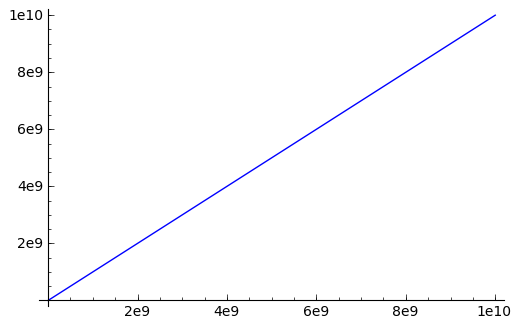
\includegraphics[height=4cm]{figures/x.png}}
	\hfill
	\subfloat[$10^x$]{\label{10hochx}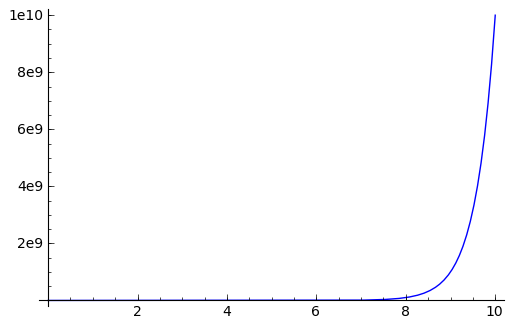
\includegraphics[height=4cm]{figures/10hochx.png}}
	\caption{Graph of the functions $x$ and $10^x$}
	\label{xund10hochx}
        \vskip +25pt 
\end{figure}


\subsubsection*{The function $\ln{x}$}
In comparison to that we consider the function $\ln{x}$. The left picture of figure \ref{lnxbis} on page \pageref{lnxbis} shows the graph with the domain of definition from $1$ to $100$. On the right picture the domain of definition was chosen between $1$ and $10^{10}$.\\
One can see that the values of the function $\ln{x}$ grow slowly compared to the growth of the function $x$. This is visualizd by the graph of both functions in one picture shown in figure \ref{xundlnxundxdurchlnx} on page \pageref{xundlnxundxdurchlnx}. In addition to that the graph of the function $\frac{x}{\ln{x}}$ was drawn in the same figure.

\begin{figure}[!htb]
	\centering
	\subfloat[ ]{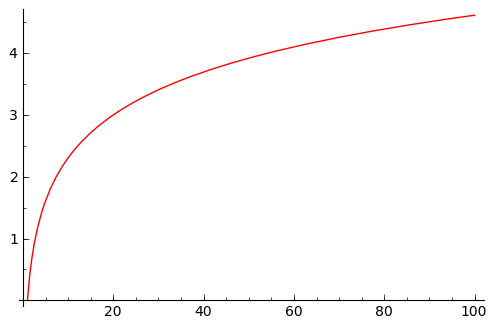
\includegraphics[height=4cm]{figures/lnxbis100.png}}
	\hfill
	\subfloat[ ]{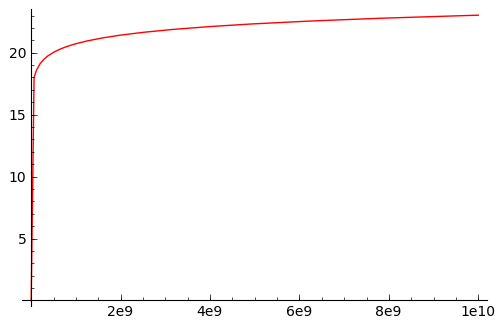
\includegraphics[height=4cm]{figures/lnxbis10hoch10.png}}
	\caption{Graph of the function $\ln{x}$ till $100$ and till $10^{10}$}
	\label{lnxbis}
        \vskip +25pt 
\end{figure}

\begin{figure}[!htb]
	\centering
	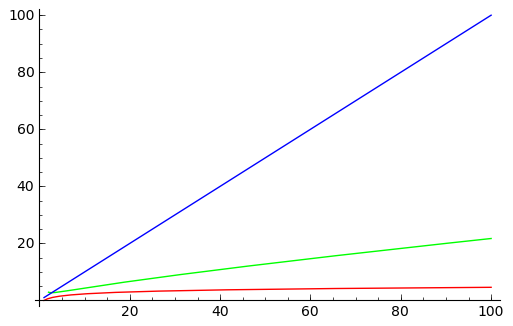
\includegraphics[height=4cm]{figures/xundlnxundxdurchlnx.png}
	\caption{The functions $x$ (blue), $\ln{x}$ (red)
                 and $\frac{x}{\ln{x}}$ (green)}
	\label{xundlnxundxdurchlnx}
        \vskip +25pt 
\end{figure}


\subsubsection*{The function $PI(x) = \frac{x}{\ln{x}}$}
\index{PI(x), $\Pi(x)$}
The function $\frac{x}{\ln{x}}$ consists of the function $x$ as the numerator and the function $\ln{x}$ in the denominator, which, in comparison to $x$, increases very slowly. Compared to the number $x$ itself, the number of primes less or equal to $x$ is small. But still, $\frac{x}{\ln{x}}$ is an increasing function as you can see in figure \ref{xundlnxundxdurchlnx} on page \pageref{xundlnxundxdurchlnx}.


\subsubsection*{The number of primes in the different intervals}
\label{primes:_Appendix_subsubsection_NumberofPrimes-in-intervals}
Figure \ref{deltazehnxdurchlnxbis}
% on page \pageref{deltazehnxdurchlnxbis}
visualizes how the number of primes in the intervals $[1, 10^x]$ and
$[10^{x-1},10^{x}]$ behave.
To calculate it faster, the result of the approximation function is used
(not the exact numbers like in the tables in chapter \ref{s:primhfk}).

Here for each base 10 exponent two bars are drawn:
$\frac{10^{x}}{\ln{10^{x}}}$ and $\frac{10^{x}}{\ln{10^{x}}}-\frac{10^{x-1}}{\ln{10^{x-1}}}$:
The left chart shows the values for the exponents $x$ from $1$ to $5$,
and the right one for $x$ from $1$ to $10$, where $x$ is the base 10 exponent.\\

The blue bars represent the overall number of primes up to $10^x$. The red bars show how many primes accrue in the interval $[10^{x-1},10^x]$, respectively.
This makes clear, that the number of primes in intervals of higher exponents keeps growing quite fast. 

\begin{figure}[!htb]
	\centering
	\subfloat[ ]{\label{deltazehnxdurchlnxbis5}
                     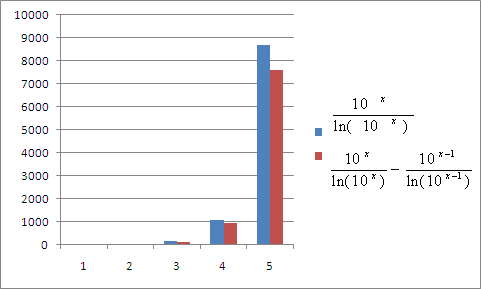
\includegraphics[height=4cm]{figures/deltazehnxdurchlnxbis5.png}}
	\hfill
	\subfloat[ ]{\label{deltazehnxdurchlnxbis10}
                     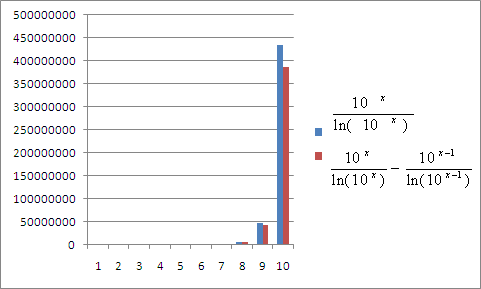
\includegraphics[height=4cm]{figures/deltazehnxdurchlnxbis10.png}}
	\caption{Numbers of primes in the interval $[1, 10^x]$ (blue) and in the
        interval $[10^{x-1},10^x]$ (red) for different exponents $x$}
	\label{deltazehnxdurchlnxbis}
\end{figure}


A table containing the number of primes in some dedicated intervals can be found
in chapter \ref{s:primhfk} at page \pageref{s:primhfk}:
For example, within the interval $[1, 10^4]$ there are 1229 primes;
thereof are in the interval $[10^3, 10^4]$ 1229 - 168 = 1061 primes.

Theory about the prime number theorem and the function PI(x) can be found in
chapter \ref{l_Primes_Distrib-of-Primes}.




\begin{sagecode}
\begin{Verbatim}%
[fontsize=\footnotesize,fontshape=tt]

# Definition of function f(x)=x and plots for the domains from 0 to 10^10 and 0 to 100
sage: def f(x):return x
....:
sage: F=plot(f,(0,10^10))
sage: F.plot()

sage: F2=plot(f,(1,100))
sage: F2.plot()


# Definition of function g(x)=10^x and plots for the domain from 0 to 10
sage: def g(x): return 10^x
....:
sage: G=plot(g,(0,10))
sage: G.plot()


# Definition of function h(x)=log(x) and plots for the domains from 1 to 100 and 1 to 10^10
sage: def h(x): return log(x)
....:
sage: H=plot(h,(1,100),color="red")
sage: H.plot()

sage: H2=plot(h,(1,10^10),color="red")
sage: H2.plot()


# Definition of function k(x)=x/log(x) and plots for the domain from 2 to 100
sage: def k(x): return x/log(x)
....:
sage: K=plot(k,(2,100),color="green")
sage: K.plot()


# Plots of the functions f, k and h for the domain of definition up to 100
sage: F2+K+H


# Generation of the data for the bar charts ..........................
# Determination of the number of primes in the interval [1,10]
sage: pari(10).primepi()-pari(1).primepi()
4

# Determination of the number of primes in the interval [10^3,10^4]
sage: pari(10**4).primepi()-pari(10**3).primepi()
1061

# Determination of the number of primes in the interval [10^8,10^9]
sage: pari(10**9).primepi()-pari(10**8).primepi()
45086079

# (for 10^10: OverflowError: long int too large to convert)

\end{Verbatim}
\caption{Generation of the graphs of the three functions x, log(x) and x/log(x)}
\end{sagecode}



% ---------------------------------------------------------------------------
% ---------------------------------------------------------------------------
\clearpage
\newpage
\hypertarget{primes:_Appendix_Sage-Samples}{}
\section{Appendix: Examples using Sage}
% \section*{Appendix A: Examples using Sage}
% \addcontentsline{toc}{section}{Appendix A: Examples using Sage}
\label{primes:_Appendix_Sage-Samples}
\index{Sage!Code examples}
\index{Sage}

\noindent Below is Sage source code related to contents of the
chapter~\ref{Label_Kapitel_Primes} (``\nameref{Label_Kapitel_Primes}''). 


% ---------------------------------------------------------------------------
% \newpage
\subsection{Some basic functions about primes using Sage}
\index{Sage}

This part of the appendix contains Sage code, to perform some simple
computations about primes.%
\footnote{See the Sage documentation about Elementary number theory
          \url{http://www.sagemath.org/doc/constructions/number_theory.html}.}

\begin{sagecode}
\begin{Verbatim}%
[fontsize=\footnotesize,fontshape=tt]

# primes (general commands)
# The set of prime numbers
sage: P=Primes(); P
Set of all prime numbers: 2, 3, 5, 7, ...

# Returns the next prime number
sage: next_prime(5)
7

# Returns how many primes <=x are there
sage: pari(10).primepi()
4

# Returns the first x primes
sage: primes_first_n(5)
[2, 3, 5, 7, 11]

# Returns the primes in an interval
sage: list(primes(1,10))
[2, 3, 5, 7]

\end{Verbatim}
\caption{Some basic functions about primes}
\end{sagecode}



% ---------------------------------------------------------------------------
\newpage
\subsection{Check primality of integers generated by quadratic functions}
\index{Sage}

The following Sage code verifies the primality of integers generated
by the function $f(n) = n^2 - 9n + 61$.
The code defines a function called \verb!quadratic_prime_formula()!
that takes three arguments:
\begin{itemize}
\item \verb!start! --- An integer which is the lower bound for
  integers in the sequence $\texttt{start}, \texttt{start} + 1,
  \texttt{start} + 2, \dots, \texttt{end} - 1, \texttt{end}$.

\item \verb!end! --- An integer which is the upper bound for the
  integers in the sequence $\texttt{start}, \texttt{start} + 1,
  \texttt{start} + 2, \dots, \texttt{end} - 1, \texttt{end}$.

\item \verb!verbose! --- (default: \verb!True!) a flag to signify
  whether to print a message indicating the primality of an integer
  generated by $f(n)$.
\end{itemize}

\noindent A meaningful modification of this code is to use another function, of
which the primality of its function values should be checked.


\begin{sagecode}
\begin{Verbatim}%
[fontsize=\footnotesize,fontshape=tt]
def quadratic_prime_formula(start, end, verbose=True):
    print "N -- N^2 - 9*N + 61"
    P = 0 # the number of primes between start and end
    for n in xrange(start, end + 1):
        X = n^2 - 9*n + 61
        if is_prime(X):
            P += 1
            if verbose:
                 print str(n) + " -- " + str(X) + " is prime"
        else:
            if verbose:
                 print str(n) + " -- " + str(X) + " is NOT prime"
    print "Number of primes: " + str(P)
    print "Percentage of primes: " + str(float((P * 100) / (end - start + 1)))
\end{Verbatim}
\caption{Verify the primality of integers generated by a quadratic function}
\end{sagecode}

\vspace{12pt}
With the following function call we compute the values of $f(n) = n^2 - 9n + 61$ for
$n = 0, 1, 2, \dots, 50$ and verify the primality of the generated integers:

\begin{Verbatim}%
[fontsize=\footnotesize,fontshape=tt]
sage: quadratic_prime_formula(0, 50)
 N -- N^2 - 9*N + 61
0 -- 61 is prime
1 -- 53 is prime
2 -- 47 is prime
3 -- 43 is prime
4 -- 41 is prime
5 -- 41 is prime
6 -- 43 is prime
7 -- 47 is prime
8 -- 53 is prime
9 -- 61 is prime
10 -- 71 is prime
11 -- 83 is prime
12 -- 97 is prime
13 -- 113 is prime
14 -- 131 is prime
15 -- 151 is prime
16 -- 173 is prime
17 -- 197 is prime
18 -- 223 is prime
19 -- 251 is prime
20 -- 281 is prime
21 -- 313 is prime
22 -- 347 is prime
23 -- 383 is prime
24 -- 421 is prime
25 -- 461 is prime
26 -- 503 is prime
27 -- 547 is prime
28 -- 593 is prime
29 -- 641 is prime
30 -- 691 is prime
31 -- 743 is prime
32 -- 797 is prime
33 -- 853 is prime
34 -- 911 is prime
35 -- 971 is prime
36 -- 1033 is prime
37 -- 1097 is prime
38 -- 1163 is prime
39 -- 1231 is prime
40 -- 1301 is prime
41 -- 1373 is prime
42 -- 1447 is prime
43 -- 1523 is prime
44 -- 1601 is prime
45 -- 1681 is NOT prime
46 -- 1763 is NOT prime
47 -- 1847 is prime
48 -- 1933 is prime
49 -- 2021 is NOT prime
50 -- 2111 is prime
Number of primes: 48
Percentage of primes: 94.1176470588
\end{Verbatim}

\noindent The last two lines of the output contain a small statistics.
You can see that $f(n)$ generates
48 primes when $0 \leq n \leq 50$, which is approximately 94\% of the
values generated by $f(n)$.\\

For larger sequences, it is impractical to print all single messages indicating
the primality of integers. In the following Sage session, only the statistics at
the end is printed (by setting the verbose parameter to false): the overall
number of primes and the percentage of primes, generated by $f(n)$ where
$0 \leq n \leq 1000$.

\begin{Verbatim}%
[fontsize=\footnotesize,fontshape=tt]
sage: quadratic_prime_formula(0, 1000, False)
N -- N^2 - 9*N + 61
Number of primes: 584
Percentage of primes: 58.3416583417
\end{Verbatim}








% --------------------------------------------------------------------------
\newpage
\begin{thebibliography}{99999}
\addcontentsline{toc}{section}{Bibliography}


\bibitem[Aaronson2003]{pr:Aaronson2003} \index{Aaronson 2003}
    Scott Aaronson, \\
    {\em The Prime Facts: From Euclid to AKS}, \\
    \url{http://www.scottaaronson.com/writings/prime.pdf} \\
    After I had completed the first edition of this article, I did come
    across the fine paper by Scott Aaronson, which also offers
    a didactically very well-done introduction to this topic. It is 
    humorous and easy to read but at the same time precise and erudite.

% already defined in elementaryNumberTheory.inc -> 2 davor
\bibitem[Bartholome1996]{pr:2Bartholome1996}  \index{Bartholome 1996}
    A. Bartholom\'e, J. Rung, H. Kern, \\     
    {\em Zahlentheorie f\"ur Einsteiger}, Vieweg, 1995, 2nd edition 1996.

\bibitem[Blum1999]{pr:Blum1999} \index{Blum 1999}   
    W. Blum, \\     
    {\em Die Grammatik der Logik}, dtv, 1999.

\bibitem[Bundschuh1998]{pr:Bundschuh1998} \index{Bundschuh 1998}
    Peter Bundschuh, \\
    {\em Einf\"uhrung in die Zahlentheorie}, Springer, 1988, 4th edition 1998.

\bibitem[Crandell2001]{pr:Crandell2001} \index{Crandell 2001} \index{Pomerance 2001}
    Richard Crandell, Carl Pomerance, \\
    {\em Prime Numbers. A Computational Perspective}, Springer, 2001.

\bibitem[Doxiadis2000]{pr:Dioxadis2000}
    Apostolos Doxiadis, \\
    {\em Uncle Petros and the Goldbach's Conjecture}, \\
    Faber/Bloomsbury, 2000.

\bibitem[Graham1989]{pr:Graham1989} \index{Graham 1989}     
   R.E. Graham, D.E. Knuth, O. Patashnik, \\
   {\em Concrete Mathematics}, Addison-Wesley, 1989.

\bibitem[Klee1997]{pr:Klee1997} \index{Klee 1997}     
   V. Klee, S. Wagon, \\
   {\em Ungel\"oste Probleme in der Zahlentheorie und der Geometrie der 
   Ebene}, \\ Birkh\"auser Verlag, 1997.

\bibitem[Knuth1981]{pr:Knuth1981} \index{Knuth 1981}     
   Donald E. Knuth, \\ 
   {\em The Art of Computer Programming, vol 2: Seminumerical Algorithms}, \\
   Addison-Wesley, 1969, 2nd edition 1981.

\bibitem[Lorenz1993]{pr:Lorenz1993} \index{Lorenz 1993}     
   F. Lorenz, \\
   {\em Algebraische Zahlentheorie}, BI Wissenschaftsverlag, 1993.

\bibitem[Oppliger2011]{pr:Oppliger2011} \index{Oppliger 2011}
    Rolf Oppliger \\
    {\em Contemporary Cryptography, Second Edition},
    Artech House, 2011, \\
    \url{http://books.esecurity.ch/cryptography2e.html}.

\bibitem[Padberg1996]{pr:Padberg1996} \index{Padberg 1996}     
   Friedhelm Padberg, \\
   {\em Elementare Zahlentheorie}, 
   Spektrum Akademischer Verlag, 1988, 2nd edition 1996.

\bibitem[Pieper1983]{pr:Pieper1983} \index{Pieper 1983}     
   H. Pieper, \\
   {\em Zahlen aus Primzahlen}, 
   Verlag Harri Deutsch, 1974, 3rd edition 1983.

\bibitem[Rempe2009]{pr:Rempe2009}  \index{Rempe 2009}
    L. Rempe, R. Waldecker, \\
    {\em Primzahltests f\"ur Einsteiger}, Vieweg+Teubner, 2009. \\
    This books results from a course for specially talented pupils at the
    ``Deutsche Sch\"ulerakademie''.
    It completely presents the AKS proof -- without expecting mathematical
    pre-knowledge.

\bibitem[Richstein1999]{pr:Richstein1999} \index{Richstein 1999}
    J. Richstein, \\
    {\em Verifying the Goldbach Conjecture up to $4*10^{14},$}
    Mathematics of Computation 70, 2001, p. 1745-1749). 

\bibitem[Scheid1994]{pr:Scheid1994} \index{Scheid 1994}
    Harald Scheid, \\ 
    {\em Zahlentheorie}, BI Wissenschaftsverlag, 2nd edition 1994.

\bibitem[Schneier1996]{pr:Schneier1996p} \index{Schneier 1996}     
    Bruce Schneier, \\
    {\em Applied Cryptography, Protocols, Algorithms, and Source Code in C},\\
    Wiley and Sons, 2nd edition 1996.

\bibitem[Schroeder1999]{pr:Schroeder1999} \index{Schroeder 1999}
    M.R. Schroeder, \\
    {\em Number Theory in Science and Communication}, \\ 
    Springer, 1984, 3rd edition 1997, Corrected Printing 1999.

\bibitem[Schwenk1996]{pr:Schwenk1996} \index{Schwenk 1996}     
    J. Schwenk \\
    {\em Conditional Access}, 
    in taschenbuch der telekom praxis, 1996, \\
    Hrgb. B. Seiler, Verlag Schiele und Sch\"on, Berlin.

\bibitem[Shoup2005]{pr:Shoup2005} \index{Shoup 2005}
    Victor Shoup \\
    {\em A Computational Introduction to Number Theory and Algebra},\\
    Cambridge University Press, 2005, \\
    \url{http://shoup.net/ntb/}.

\bibitem[Tietze1973]{pr:Tietze1973} \index{Tietze 1973}     
    H. Tietze, \\
    {\em Gel\"oste und ungel\"oste mathematische Probleme}, \\
    Verlag C. H. Beck, 1959, 6th edition 1973.

\end{thebibliography}


% --------------------------------------------------------------------------
\newpage
% \section*{Web links} \addcontentsline{toc}{section}{Web links}
\chapter*{Web links} \addcontentsline{toc}{section}{Web links}

\begin{enumerate}
\item GIMPS (Great Internet Mersenne-Prime Search) 
      \index{Mersenne!prime number}  \index{GIMPS} \\
      www.mersenne.org is the home page of the GIMPS project, \\
      \url{http://www.mersenne.org/prime.htm}

\item The Proth Search Page with the Windows program by Yves Gallot \\
      \url{http://www.utm.edu/research/primes/programs/gallot/index.html}

\item Generalized Fermat Prime Search \\
      \url{http://primes.utm.edu/top20/page.php?id=12}

\item Distributed Search for Fermat Number Divisors \\
      \url{http://www.fermatsearch.org/}

\item At the University of Tennessee you will find extensive research
      results about prime numbers. \\
      \url{http://www.utm.edu/}

\item The best overview about prime numbers is offered from my point of view 
      by ~``The Prime Pages'' from professor Chris Caldwell.
      \index{Caldwell Chris} \\
      \url{http://www.utm.edu/research/primes}

\item Descriptions e.g.\ about prime number tests \\
      \url{http://www.utm.edu/research/primes/mersenne.shtml} \\
      \url{http://www.utm.edu/research/primes/prove/index.html}

\item Showing the $n$-th prime number P(n)\\
      \url{http://www.utm.edu/research/primes/notes/by_year.html}

\item The supercomputer manufacturer SGI Cray Research not only 
      employed brilliant mathematicians but also used the prime 
      number tests as benchmarks for its machines. \\
      \url{http://www.isthe.com/chongo/tech/math/prime/prime_press.html}
	 
\item The Cunningham Project, \index{Cunningham project}\\ 
      \url{http://www.cerias.purdue.edu/homes/ssw/cun/}

\item \url{http://www.eff.org/awards/coop}

% \item \url{http://www.informatik.tu-darmstadt.de/TI/LiDIA/}

\item \url{http://www.math.Princeton.EDU/~arbooker/nthprime.html}
% {\tt http://www.math.Princeton.EDU/\~{}arbooker/nthprime.html }

\item Goldbach conjecture verification project von Tom�s Oliveira e Silva,
      \index{Goldbach project}\\ 
      \url{http://www.ieeta.pt/~tos/goldbach.html}

\item \url{http://www.mathematik.ch/mathematiker/goedel.html}

\end{enumerate}




\vskip +10 pt
% --------------------------------------------------------------------------
\section*{Acknowledgments}
\addcontentsline{toc}{section}{Acknowledgments}

I would like to take this opportunity to thank Mr.\ Henrik Koy and Mr.\ Roger
Oyono for their very constructive proof-reading of the first versions
of this article.



% Local Variables:
% TeX-master: "../script-en.tex"
% End:

\renewcommand{\CTBChapName}{(Chap NT)}            % $Id$
%\def\QM {{,\kern -0.9 pt ,}}
\setcounter{satz}{0}
\setcounter{definition}{0}

% ..........................................................................
% --------------------------------------------------------------------------
% ++++++++++++++++++++++++++++++++++++++++++++++++++++++++++++++++++++++++++
%              E l e m e n t a r e  Z a h l e n t h e o r i e
% /~~~~~~~~~~~~~~~~~~~~~~~~~~~~~~~~~~~~~~~~~~~~~~~~~~~~~~~~~~~~~~~~~~~~~~~~~

\hypertarget{Chapter_ElementaryNT}{}
\chapter{Einf�hrung in die elementare Zahlentheorie mit Beispielen}
\label{Chapter_ElementaryNT}
(Bernhard Esslinger, Juli 2001; Updates: Nov. 2001, Juni 2002, Mai 2003,
 Mai 2005, M�rz 2006, Juni 2007, Juli 2009) \\

Diese \glqq Einf�hrung\grqq~ bietet einen Einstieg f�r mathematisch Interessierte.
Erforderlich sind nicht mehr Vorkenntnisse als die, die im Grundkurs Mathematik am Gymnasium vermittelt werden.\par
Wir haben uns bewusst an \glqq Einsteigern\grqq~ und \glqq Interessenten\grqq~ orientiert, und nicht an den
Gepflogenheiten mathematischer Lehrb�cher, die auch dann \glqq Einf�hrung\grqq~ genannt werden,
wenn sie schon auf der 5. Seite nicht mehr auf Anhieb zu verstehen sind und sie eigentlich den Zweck haben, dass
man danach auch spezielle Monographien zu dem Thema lesen k�nnen soll.



% ++++++++++++++++++++++++++++++++++++++++++++++++++++++++++++++++++++++++++
\section{Mathematik und Kryptographie}
Ein gro�er Teil der modernen, asymmetrischen Kryptographie beruht auf 
mathematischen Erkenntnissen -- auf den Eigenschaften (\glqq Gesetzen'')
ganzer Zahlen, die in der elementaren \index{Zahlentheorie!elementare}
Zahlentheorie untersucht werden. \glqq Elementar\grqq\ bedeutet hier, 
dass die zahlentheoretischen Fragestellungen im wesentlichen
in der Menge der nat�rlichen und der ganzen Zahlen durchgef�hrt werden.

Weitere mathematische Disziplinen, die heute in der Kryptographie 
Verwendung finden, sind 
(vgl. \cite[S. 2]{nt:Bauer1995}, \cite[Seite 3]{nt:Bauer2000}) :
\begin{itemize}
    \item Gruppentheorie
    \item Kombinatorik
    \item Komplexit�tstheorie
    \item Ergodentheorie
    \item Informationstheorie.
\end{itemize}

Die Zahlentheorie oder Arithmetik (hier wird mehr der Aspekt des Rechnens
mit Zahlen betont) wurde von Carl Friedrich Gauss\footnote{%
  Carl Friedrich Gauss, deutscher Mathematiker und Astronom,
  30.4.1777$-$23.2.1855.
}
\index{Gauss, Carl Friedrich}
als besondere mathematische Disziplin begr�ndet. Zu ihren elementaren
Gegenst�nden geh�ren: gr��ter gemeinsamer Teiler\footnote{%
Auf ggT\index{ggT}, englisch gcd (greatest common divisor), geht dieser
Artikel in Anhang~\ref{NumberTheory_Appendix_GCD} ein.
} (ggT), Kongruenzen (Restklassen), Faktorisierung, Satz von Euler-Fermat und
primitive Wurzeln. Kernbegriff sind jedoch die Primzahlen und ihre
multiplikative Verkn�pfung.

Lange Zeit galt gerade die Zahlentheorie als Forschung pur, als
Paradebeispiel f�r die Forschung im Elfenbeinturm. Sie erforschte die
\glqq geheimnisvollen Gesetze im Reich der Zahlen'' und gab Anlass zu
philosophischen Er�rterungen, ob sie beschreibt, was �berall in der Natur
schon da ist, oder ob sie ihre Elemente (Zahlen, Operatoren, Eigenschaften)
nicht k�nstlich konstruiert.

Inzwischen wei� man, dass sich zahlentheoretische Muster �berall in der Natur
finden. Zum Beispiel verhalten sich die Anzahl der links- und der
rechtsdrehenden Spiralen einer Sonnenblume zueinander wie zwei
aufeinanderfolgende\index{Fibonacci} Fibonacci-Zahlen\footnote{%
Die Folge der Fibonacci-Zahlen $(a_i)_{i \in \mathbb{N}}$ ist definiert durch die \glqq rekursive'' 
Vorschrift $a_1 := a_2 := 1$ und f�r alle Zahlen  $n=1,2,3,\cdots$ definiert man 
$a_{n+2} := a_{n+1}+a_n$.  Zu dieser historischen Folge gibt es viele interessante 
Anwendungen in der Natur (siehe z.B. \cite[S. 290 ff]{nt:Graham1994}\index{Graham 1994} oder die Web-Seite 
von \hyperlink{knott}{Ron Knott:} \index{Knott, Ron} hier dreht sich alles um Fibonacci-Zahlen). 
Die Fibonacci-Folge\index{Fibonacci} ist gut verstanden und wird heute als wichtiges Werkzeug in der 
Mathematik benutzt.
}, also z.B.  wie  $21 : 34$.

Au�erdem wurde sp�testens mit den zahlentheoretischen Anwendungen der
modernen Kryptographie klar, dass eine jahrhundertelang als theoretisch
geltende Disziplin praktische Anwendung findet, nach deren Experten heute
eine hohe Nachfrage auf dem Arbeitsmarkt besteht.

Anwendungen der (Computer-)Sicherheit bedienen sich heute der Kryptographie,
weil Kryptographie als mathematische Disziplin einfach besser und
beweisbarer ist als alle im Laufe der Jahrhunderte erfundenen \glqq kreativen''
Verfahren der Substitution und besser als alle ausgefeilten physischen
Techniken wie beispielsweise beim Banknotendruck \cite[S. 4]{nt:Beutelspacher1996}.

In diesem Artikel werden in einer leicht verst�ndlichen Art die
grundlegenden Erkenntnisse der elementaren Zahlentheorie anhand vieler
Beispiele vorgestellt -- auf Beweise wird (fast) vollst�ndig verzichtet
(diese finden sich in den mathematischen Lehrb�chern).

Ziel ist nicht die umfassende Darstellung der zahlentheoretischen Erkenntnisse,
sondern das Aufzeigen der wesentlichen Vorgehensweisen. Der Umfang des Stoffes
orientiert sich daran, das RSA-Verfahren\index{RSA} verstehen und anwenden
zu k�nnen.

Dazu wird sowohl an Beispielen als auch in der Theorie erkl�rt, wie man in
endlichen Mengen rechnet und wie dies in der Kryptographie Anwendung findet.
Insbesondere wird auf die klassischen Public-Key-Verfahren Diffie-Hellman
\index{Diffie-Hellman} (DH) und RSA\index{RSA} eingegangen.

Au�erdem war es mir wichtig, fundierte Aussagen zur Sicherheit des RSA-Verfahrens zu machen.



\vskip +40 pt

\begin{center}
\fbox{\parbox{15cm}{{\em Carl Friedrich Gauss:\index{Gauss, Carl Friedrich}}\\
Die Mathematik ist die K�nigin der Wissenschaften, die Zahlentheorie aber
ist die K�nigin der Mathematik.}}
\end{center}

% ++++++++++++++++++++++++++++++++++++++++++++++++++++++++++++++++++++++++++
\section{Einf�hrung in die Zahlentheorie}
\index{Zahlentheorie!Einf�hrung} 

Die Zahlentheorie entstand aus Interesse an den positiven ganzen Zahlen $1,
2, 3, 4, \cdots ,$ die auch als die Menge der \index{Zahlen!nat�rliche}
{\em nat�rlichen Zahlen} $\mathbb{N}$ bezeichnet
werden. Sie sind die ersten mathematischen Konstrukte der menschlichen
Zivilisation. Nach Kronecker\footnote{%
Leopold Kronecker, deutscher Mathematiker, 7.12.1823$-$29.12.1891.
}
\index{Kronecker, Leopold} hat sie der liebe Gott geschaffen, 
nach Dedekind\footnote{Julius Wilhelm Richard Dedekind,
deutscher Mathematiker, 06.10.1831$-$12.02.1916.
}
\index{Dedekind, Julius} der menschliche Geist.
Das ist je nach Weltanschauung ein unl�sbarer Widerspruch oder
ein und dasselbe.

Im Altertum gab es keinen Unterschied zwischen Zahlentheorie und
Numerologie, die einzelnen Zahlen mystische Bedeutung zuma�. So wie sich
w�hrend der Renaissance (ab dem 14. Jahrhundert) die Astronomie allm�hlich
von der Astrologie und die Chemie von der Alchemie l�ste, so lie� auch die
Zahlentheorie die Numerologie hinter sich.

Die Zahlentheorie faszinierte schon immer Amateure wie auch professionelle
Mathematiker. Im Unterschied zu anderen Teilgebieten der Mathematik k�nnen
viele der Probleme und S�tze auch von Laien verstanden werden, andererseits
widersetzten sich die L�sungen zu den Problemen und die Beweise zu den S�tzen
oft sehr lange den Mathematikern. Es ist also leicht, gute Fragen zu stellen,
aber es ist ganz etwas anderes, die Antwort zu finden. Ein Beispiel daf�r ist
der sogenannte letzte (oder gro�e) Satz von Fermat\footnote{Thema der
   Schul-Mathematik ist der Satz von Pythagoras\index{Pythagoras!Satz von},
   wo gelehrt wird, dass in einem rechtwinkligen Dreieck gilt:
   $a^2 + b^2 = c^2$, wobei $a, b$ die Schenkell�ngen sind und 
   c die L�nge der Hypothenuse ist.
   Fermats ber�hmte Behauptung war, dass f�r $a,b,c \in \mathbb{N}$ und
   f�r ganzzahlige Exponenten $n > 2$ immer die Ungleichheit
   $a^n + b^n \not= c^n$ gilt.  Leider fand \index{Fermat!letzter Satz}
   Fermat auf dem Brief, wo er die Behauptung aufstellte, nicht gen�gend
   Platz, um den Satz zu beweisen. Der Satz konnte erst �ber 300 Jahre sp�ter
   bewiesen werden \cite[S. 433-551]{nt:Wiles1994}. \index{Wiles, Andrew}
}.

Bis zur Mitte des 20. Jahrhunderts wurde die Zahlentheorie als das reinste
Teilgebiet der Mathematik angesehen -- ohne Verwendung in der wirklichen Welt.
Mit dem Aufkommen der Computer und der digitalen Kommunikation �nderte sich
das: die Zahlentheorie konnte einige unerwartete Antworten f�r reale
Aufgabenstellungen liefern. Gleichzeitig halfen die Fortschritte in der EDV,
dass die Zahlentheoretiker gro�e Fortschritte machten im Faktorisieren gro�er
Zahlen, in der Bestimmung neuer Primzahlen, im Testen von (alten)
Vermutungen und beim L�sen bisher unl�sbarer numerischer Probleme.

Die moderne Zahlentheorie \index{Zahlentheorie!moderne} besteht aus Teilgebieten wie
\begin{itemize}
    \item Elementare Zahlentheorie
    \item Algebraische Zahlentheorie
    \item Analytische Zahlentheorie
    \item Geometrische Zahlentheorie
    \item Kombinatorische Zahlentheorie
    \item Numerische Zahlentheorie und
    \item Wahrscheinlichkeitstheorie.
\end{itemize}

Die verschiedenen Teilgebiete besch�ftigen sich alle mit Fragestellungen zu
den ganzen Zahlen (positive und negative ganze Zahlen und die Null), gehen
diese jedoch mit verschiedenen Methoden an.

Dieser Artikel besch�ftigt sich nur mit dem Teilgebiet der elementaren
Zahlentheorie.
\newpage


% --------------------------------------------------------------------------
\subsection{Konvention}
Wird nichts anderes gesagt, gilt: 
\begin{itemize}
\item Die Buchstaben $a, b, c, d, e, k, n, m, p, q$ stehen f�r ganze Zahlen.
\item Die Buchstaben $i$ ~\mbox{und} ~$j$ stehen f�r nat�rliche Zahlen. 
\item Der Buchstabe $p$ steht stets f�r eine Primzahl.
\item Die Mengen $\mathbb{N} = \{ 1, 2, 3, \cdots \}$ und $\mathbb{Z} =\{ \cdots, -3, -2, -1, 0, 1, 2, 3, \cdots \}$ 
sind die {\em nat�rlichen} und die {\em ganzen} Zahlen.
\end{itemize}



%\vskip +40 pt
\newpage

\begin{center}
\fbox{\parbox{15cm}{{\em Joanne K. Rowling\index{Rowling, Joanne}\footnotemark:}\newline Das ist nicht Zauberei, das ist Logik, ein R�tsel.
Viele von den gr��ten Zauberern haben keine Unze Logik im Kopf.}}
\end{center}
\addtocounter{footnote}{0}\footnotetext{Joanne K. Rowling,~\glqq Harry Potter und der Stein der Weisen'', Carlsen, (c)
1997, Kapitel ~\glqq Durch die Fallt�r'', S. 310, Hermine.}


% ++++++++++++++++++++++++++++++++++++++++++++++++++++++++++++++++++++++++++
\section{Primzahlen und der erste Hauptsatz der elementaren Zahlentheorie}
\index{Zahlentheorie!elementare} Viele der Probleme in der elementaren
Zahlentheorie besch�ftigen sich mit Primzahlen.

Jede ganze Zahl hat Teiler oder Faktoren. Die Zahl 1 hat nur einen, n�mlich
sich selbst. Die Zahl 12 hat die sechs Teiler 1, 2, 3, 4, 6 und 12\footnote{%
Aufgrund der gro�en Teilerzahl von 12 findet sich diese Zahl -- und Vielfache dieser Zahl -- oft im allt�glichen wieder:
Die 12 Stunden-Skala der Uhr, die 60 Minuten einer Stunde, die 360 Grad-Skala der Winkelmessung, usw. Teilt man 
diese Skalen in Bruchteile auf, so ergeben sich in vielen F�llen die Br�che als ganze Zahlen. Mit diesen kann 
man im Kopf einfacher rechnen als mit gebrochenen Zahlen.
}. Viele Zahlen sind nur teilbar durch sich selbst und durch 1. Bez�glich der
Multiplikation sind dies die \glqq Atome'' im Bereich der Zahlen.

\index{Primzahl}
\begin{definition}\label{def-zth-prime} 
{\bf Primzahlen} sind nat�rliche Zahlen gr��er als $1$, die nur durch $1$ und sich
selbst teilbar sind.
\end{definition}

Per Definition ist $1$ keine Primzahl.

Schreibt man die Primzahlen in aufsteigender Folge (Primzahlenfolge), so
ergibt sich
$$2,~ 3,~ 5,~ 7,~ 11, ~13,~ 17,~ 19, ~23, ~29, ~31, ~37,~ 41,~ 43,~ 47,~ 53, ~59, ~61, ~67, ~71,
~73, ~79, ~83, ~89, ~97, \cdots.$$

Unter den ersten $100$ Zahlen gibt es genau $25$ Primzahlen. Danach nimmt ihr
prozentualer Anteil ab, wird aber nie Null.

Primzahlen treten als ganze Zahlen nicht selten auf. Allein im letzten
Jahrzehnt waren drei Jahre prim: $1993, 1997$ und $1999$. W�ren sie selten,
k�nnte die Kryptographie auch nicht so mit ihnen arbeiten, wie sie es tut.

Primzahlen k�nnen nur auf eine einzige (\glqq triviale'') Weise zerlegt werden:
\begin{eqnarray*}
5 & = & 1 * 5 \nonumber \\
17 & =  & 1 * 17 \nonumber \\
1.013 &  = & 1 * 1013 \nonumber \\
1.296.409 & = & 1 * 1.296.409. \nonumber
\end{eqnarray*}

\index{Zahlen!zusammengesetzte}
\begin{definition}\label{def-zth-composite} 
Nat�rliche Zahlen gr��er $1$, die keine Primzahlen sind, hei�en
{\bf zusammengesetzte Zahlen}: Diese haben mindestens zwei von $1$ verschiedene
Faktoren.
\end{definition}


\begin{example}{ Primfaktorzerlegung\index{Primfaktor!Zerlegung} solcher Zahlen:}
\begin{eqnarray*}
4 & = & 2*2  \nonumber \\
6 & = & 2*3  \nonumber \\
91 & = & 7*13  \nonumber \\
161 & = & 7*23  \nonumber \\
767 & = & 13*59  \nonumber \\
1.029 & = & 3 * 7^3  \nonumber \\
5.324 & = & 22 * 11^3.  \nonumber 
\end{eqnarray*}

\begin{satz}\label{thm-zth-cnum}
Jede zusammengesetzte Zahl $a$ besitzt einen kleinsten Teiler gr��er
als $1$. Dieser Teiler ist eine Primzahl $p$ und kleiner oder gleich der Quadratwurzel
aus $a$.
\end{satz}
\end{example}
Aus den Primzahlen lassen sich alle ganzen Zahlen gr��er als $1$
zusammensetzen -- und das sogar in einer {\em eindeutigen} Weise.

Dies besagt \index{Zahlentheorie!Hauptsatz} der 1. {\em Hauptsatz der Zahlentheorie} (= Hauptsatz der elementaren
Zahlentheorie = fundamental theorem of arithmetic = fundamental building
block of all positive integers). Er wurde das erste Mal pr�zise von Carl
Friedrich Gauss in seinen Disquisitiones Arithmeticae (1801) formuliert. 
\index{Zahlentheorie!Hauptsatz}  \index{Gauss, Carl Friedrich}

\begin{satz}{\bf Gauss 1801}\label{thm-zth-mthm}
Jede nat�rliche Zahl $a$ gr��er als $1$ l�sst sich als Produkt von
Primzahlen schreiben. Sind zwei solche Zerlegungen $a = p_1*p_2*\cdots*p_n = q_1*q_2*\cdots*q_m$ gegeben, dann
gilt nach eventuellem Umsortieren $n = m$ und f�r alle $i$: $p_i = q_i$.
\end{satz}

In anderen Worten: Jede nat�rliche Zahl au�er der $1$ l�sst sich auf genau eine
Weise als Produkt von Primzahlen schreiben, wenn man von der Reihenfolge der
Faktoren absieht. Die Faktoren sind also eindeutig (die \glqq Expansion in
Faktoren'' ist eindeutig)!

Zum Beispiel ist $60 = 2*2*3*5 = 2^2*3*5$. Und das ist --- bis auf eine
ver�nderte Reihenfolge der Faktoren --- die einzige M�glichkeit, die Zahl $60$
in Primfaktoren\index{Primfaktor} zu zerlegen.

Wenn man nicht nur Primzahlen als Faktoren zul�sst, gibt es mehrere
M�glichkeiten der Zerlegung in Faktoren und die {\em Eindeutigkeit} (uniqueness)
geht verloren:
$$60 = 1*60 = 2*30 = 4*15 = 5*12 = 6*10 = 2*3*10 = 2*5*6 = 3*4*5 = \cdots$$
Der 1. Hauptsatz ist nur scheinbar selbstverst�ndlich. Man kann viele andere
Zahlenmengen\footnote{%
Diese Mengen werden speziell aus der Menge der nat�rlichen Zahlen gebildet.
Ein Beispiel findet sich in diesem \hyperlink{uniqueness}{Skript}
auf Seite~\pageref{thm-pz-euklid} %eigentlich \pageref{remFundTheoOfArithm},
%aber hyperref ist buggy
am Ende von Kapitel~\ref{primesinmath}.
}
konstruieren, bei denen eine multiplikative Zerlegung in die Primfaktoren
dieser Mengen {\em nicht} eindeutig ist.

F�r eine mathematische Aussage ist es deshalb nicht nur wichtig, f�r welche
Operation sie definiert wird, sondern auch auf welcher Grundmenge diese
Operation definiert wird.

Weitere Details zu den Primzahlen (z.B. wie der \glqq Kleine Satz von 
Fermat'' zum Testen von sehr gro�en Zahlen auf ihre Primzahleigenschaft
benutzt werden kann) finden sich in diesem Skript in dem Artikel �ber 
\hyperlink{Kapitel_2}{Primzahlen, Kapitel~\ref{Label_Kapitel_2}}.


% ++++++++++++++++++++++++++++++++++++++++++++++++++++++++++++++++++++++++++
\section[Teilbarkeit, Modulus und Restklassen]
           {Teilbarkeit, Modulus und Restklassen\footnotemark}
\footnotetext{%
    \index{ZT, Lernprogramm Zahlentheorie}%
    \index{Lernprogramm ZT}%
    Mit dem Lernprogramm {\bf ZT} k�nnen Sie das hier und im Folgekapitel
    vorgestellte Rechnen mit Kongruenzen spielerisch nachvollziehen
    (siehe Lern-Kapitel 2.1, Seiten 2-9/40).\\
    ZT k�nnen Sie in CrypTool\index{CrypTool} �ber das Men�
    {\bf Einzelverfahren \textbackslash{} Zahlentheorie
    interaktiv \textbackslash{} Lernprogramm f�r Zahlentheorie} aufrufen.
    Siehe Anhang~\ref{s:appendix-Learn-NT}.
}
\index{Modulus} \index{Teilbarkeit}
Werden ganze Zahlen addiert, subtrahiert oder multipliziert, ist das
Ergebnis stets wieder eine ganze Zahl.

Die Division zweier ganzer Zahlen ergibt nicht immer eine ganze Zahl. Wenn
man z.B. $158$ durch $10$ teilt, ist das Ergebnis die Dezimalzahl $15,8$.
Dies ist keine ganze Zahl!

Teilt man $158$ dagegen durch $2$, ist das Ergebnis $79$ eine ganze Zahl.
In der Zahlentheorie sagt man, $158$ ist {\em teilbar} durch $2$, aber nicht durch $10$.
Allgemein sagt man:

\begin{definition}\label{def-zth-divisibility} \index{Teilbarkeit}
Eine ganze Zahl $n$ ist {\bf teilbar} durch eine ganze Zahl $d$, wenn der Quotient $n/d$
eine ganze Zahl $c$ ist, so dass $n = c * d$.
\end{definition}

Die Zahl $n$ wird {\em Vielfaches} von $d$ genannt; $d$ wird {\em Teiler, Divisor} \index{Teiler} \index{Divisor} oder \index{Faktor} {\em Faktor} von $n$
genannt.

Mathematisch schreibt man das: $d | n$ (gelesen: \glqq  $d$ teilt $n$'').
Die Schreibweise $d \!\!\not| n$ bedeutet, dass $d$ die Zahl $n$ nicht teilt.

Also gilt in unserem obigen Beispiel: $10\!\!\not| 158$, aber $2 | 158$.


% --------------------------------------------------------------------------
\subsection{Die Modulo-Operation -- Rechnen mit Kongruenzen} \index{Kongruenz}

Bei Teilbarkeitsuntersuchungen kommt es nur auf die Reste der Division an:
Teilt man eine Zahl $n$ durch $m$, so benutzt man oft die folgende Schreibweise:
$$\frac{n}{m} = c + \frac{r}{m} ,$$
wobei $c$ eine ganze Zahl ist und $r$ eine Zahl mit den Werten $0,1,\cdots, m-1$.
Diese Schreibweise hei�t Division mit Rest. Dabei hei�t $c$ der ganzzahlige 
\glqq Quotient'' und $r$ der \glqq Rest'' der Division.

\begin{example}{:}
$$\frac{19}{7} = 2 + \frac{5}{7} \quad (m=7, c = 2, r = 5)$$
\end{example}
Was haben die Zahlen $5, 12, 19, 26, \cdots$ bei der Division durch $7$ gemeinsam?
Es ergibt sich immer der Rest $r = 5$.
Bei der Division durch $7$ sind nur die folgenden Reste m�glich:
$$r = 0, 1, 2, \cdots, 6.$$

Wir fassen bei der Division durch $7$ die Zahlen, die den gleichen Rest $r$
ergeben, in die \glqq Restklasse $r$ modulo $7$'' zusammen. Zwei Zahlen $a$ und $b$, die
zur gleichen Restklasse modulo $7$ geh�ren, bezeichnen wir als \glqq kongruent
modulo 7''. Oder ganz allgemein:

\begin{definition}\label{def-zth-remainder} \index{Restklasse}
Als {\bf Restklasse $r$ modulo $m$} bezeichnet man alle ganzen Zahlen $a$, die bei der Division 
durch $m$ denselben Rest $r$ haben.
\end{definition}
\newpage
\begin{example}{:}
\begin{itemize}
\item[] Restklasse $0$ modulo $4 = \{ x | x = 4*n; \; n \in \mathbb{Z} \} = \{ \dots, -16, -12, -8, -4, 0, 4, 8, 12, 16, \dots \}$
\item[] Restklasse $3$ modulo $4 = \{ x | x = 4*n + 3;\; n \in \mathbb{Z} \} = \{ \dots, -13, -9, -5, -1, 3, 7, 11, 15, \dots \}$
\end{itemize}
\end{example}
Da modulo $m$ nur die Reste $0, 1, 2, \cdots, m-1$ m�glich sind, rechnet die modulare Arithmetik in endlichen Mengen. 
Zu jedem Modul $m$ gibt es genau $m$ Restklassen.

\begin{definition}\label{def-zth-congruence} \index{Kongruenz}
Zwei Zahlen $a, b \in \mathbb{N}$  hei�en \index{restgleich}
{\bf restgleich oder kongruent bez�glich $m \in \mathbb{N}$}  genau dann, 
wenn beim Teilen durch $m$ der gleiche Rest bleibt.
\end{definition}

Man schreibt: $a \equiv b {\rm ~(mod~} m)$. Und sagt:  {\em $a$ ist kongruent $b$ modulo $m$}. Das bedeutet, 
dass $a$ und $b$ zur gleichen Restklasse geh�ren. Der Modul ist also der Teiler. Diese Schreibweise wurde von 
Gauss eingef�hrt. Gew�hnlich ist der Teiler positiv, aber $a$ und $b$ k�nnen auch beliebige ganze Zahlen sein.

\begin{example}{:}
\begin{itemize}
   \item[] $19 \equiv 12 {\rm ~(mod~} 7)$,         
           denn die Reste sind gleich:  $19 / 7 = 2$ Rest $5$  und  $12 / 7 = 1$ Rest $5$.
   \item[] $23103 \equiv 0 {\rm ~(mod~} 453)$, denn $23103 / 453 = 51$ Rest $0$  und  $0 / 453 = 0$ Rest $0$.
\end{itemize}
\end{example}

\begin{satz}\label{thm-zth-div}
$a \equiv b$ (mod $m$) gilt genau dann,  wenn die Differenz $(a - b)$ durch $m$ teilbar ist, also wenn 
ein $q\in \mathbf{Z}$ existiert mit $ (a-b)=q*m.$
\end{satz}
Diese beiden Aussagen sind also �quivalent.

Daraus ergibt sich: Wenn $m$ die Differenz teilt, gibt es eine ganze Zahl $q$, so dass gilt: $a = b + q*m$.
Alternativ zur Kongruenzschreibweise kann man auch die Teilbarkeitsschreibweise verwenden: $m | (a - b)$.

\begin{example}{ f�r �quivalente Aussagen:} \\
$35 \equiv 11$ (mod $3) \Longleftrightarrow  35 - 11 \equiv 0$ (mod $3)$, 
wobei $35 - 11 = 24$ sich ohne Rest durch $3$ teilen l�sst, w�hrend $35:3$ und $11:3$ beide den Rest $2$ ergeben.
\end{example}

\begin{remark}{:}\\
F�r die Summe $(a + b)$ gilt die obige �quivalenz nicht!
\end{remark}

\begin{example}{:}\\
$11 \equiv 2$ (mod $3$), also ist $11 - 2 = 9 \equiv 0$ (mod $3$); aber $11 + 2 = 13$ ist nicht durch $3$ teilbar.
\end{example}

Die Aussage von Satz~\ref{thm-zth-div} gilt f�r Summen nicht einmal in eine
Richtung. Richtig ist sie bei Summen nur f�r den Rest $0$ und nur in der
folgenden Richtung: Teilt ein Teiler beide Summanden ohne Rest, teilt er
auch die Summe ohne Rest.


Anwenden kann man die obige �quivalenz von Satz~\ref{thm-zth-div}, wenn man schnell und
geschickt f�r gro�e Zahlen entscheiden will, ob sie durch eine bestimmte
Zahl teilbar sind.

\newpage
\begin{example}{:} \\
Ist $69.993$ durch $7$ teilbar?\\
Da die Zahl in eine Differenz zerlegt werden kann, wo einfach zu ersehen
ist, dass jeder Operand durch $7$ teilbar ist, ist auch die Differenz durch $7$
teilbar: $69.993 = 70.000 - 7$.
\end{example}

Diese �berlegungen und Definitionen m�gen recht theoretisch erscheinen, sind
uns im Alltag aber so vertraut, dass wir die formale Vorgehensweise gar nicht
mehr wahrnehmen: Bei der Uhr werden die $24$ h eines Tages durch die Zahlen $1$,
$2, \cdots, 12$ repr�sentiert. Die Stunden nach $12:00$ mittags erh�lt man als
Reste einer Division durch 12. Wir wissen sofort, dass $2$ Uhr nachmittags
dasselbe wie $14:00$ ist.

Diese \glqq modulare'', also auf die Divisionsreste bezogene Arithmetik ist die
Basis der asymmetrischen Verschl�sselungsverfahren.
Kryptographische Berechnungen spielen sich also nicht wie das Schulrechnen
unter den reellen Zahlen ab, sondern unter Zeichenketten begrenzter L�nge,
das hei�t unter positiven ganzen Zahlen, die einen gewissen Wert nicht
�berschreiten d�rfen.
Aus diesem und anderen Gr�nden w�hlt man sich eine gro�e Zahl $m$ und \glqq rechnet
modulo $m$'', das hei�t, man ignoriert ganzzahlige Vielfache von $m$ und rechnet
statt mit einer Zahl nur mit dem Rest bei Division dieser Zahl durch $m$.
Dadurch bleiben alle Ergebnisse im Bereich von $0$ bis $m-1$.


% ++++++++++++++++++++++++++++++++++++++++++++++++++++++++++++++++++++++++++
\section{Rechnen in endlichen Mengen}

% --------------------------------------------------------------------------
\subsection{Gesetze beim modularen Rechnen}

Aus S�tzen der Algebra folgt, dass wesentliche Teile der �blichen
Rechenregeln beim �bergang zum modularen Rechnen �ber der Grundmenge $\mathbb{Z}$
erhalten bleiben: Die Addition ist nach wie vor kommutativ. Gleiches gilt f�r die
Multiplikation modulo $m$. Das Ergebnis einer Division\footnote{%
\label{ftn-res-divmodn}
Die Division modulo $m$\index{Division modulo $n$}
ist nur f�r Zahlen, die teilerfremd\index{Zahlen!teilerfremd (co-prime)}
zu $m$ sind, definiert, da andere Zahlen die gleiche Eigenschaft wie Null haben.
Vergleiche Fu�snote~\ref{ftn-mod6} in Kapitel~\ref{addmult}.
} ist kein Bruch, sondern eine ganze Zahl zwischen $0$ und $m-1$.

\noindent Es gelten die bekannten Gesetze:
\begin{itemize}
\item[\bf 1.] {\bf Assoziativgesetz:}\index{Assoziativgesetz} \\ 
    $((a+b) + c) {\rm ~(mod~ } m) \equiv  (a + (b+c)) {\rm ~(mod~ } m).$ \\
    $((a*b) * c) {\rm ~(mod~ } m) \equiv  (a * (b*c)) {\rm ~(mod~ } m).$
\item[\bf 2.] {\bf Kommutativgesetz:} \index{Kommutativgesetz}\\
    $(a+b) {\rm ~(mod~ } m) \equiv  (b+a) {\rm ~(mod~ } m).$ \\
     $(a*b) {\rm ~(mod~ } m) \equiv  (b*a) {\rm ~(mod~ } m).$
\end{itemize}
Assoziativgesetz und Kommutativgesetz gelten sowohl f�r die Addition als auch f�r die Multiplikation.
\begin{itemize}
\item[\bf 3.] {\bf Distributivgesetz:} \index{Distributivgesetz}\\
    $ (a * (b+c)) {\rm ~(mod~ } m) \equiv  (a*b + a*c) {\rm ~(mod~ } m).$ 
\item[\bf 4.] {\bf Reduzierbarkeit:} \index{Reduzierbarkeit} \\
    $(a+b) {\rm ~(mod~} m) \equiv  (a {\rm ~(mod~ } m) + b {\rm ~(mod~ } m)) {\rm ~(mod~} m).$ \\  
    $(a*b) {\rm ~(mod~} m) \equiv  (a {\rm ~(mod~ } m) * b {\rm ~(mod~ } m)) {\rm ~(mod~} m).$ \\
    Beim Addieren und Multiplizieren ist es gleichg�ltig, in welcher Reihenfolge die Modulo-Operation durchgef�hrt wird.
\end{itemize}
\begin{itemize}
\item[\bf 5.] {\bf Existenz einer Identit�t (neutrales Element):} \index{Identit�t}\\
    $(a + 0) {\rm ~(mod~ } m) \equiv  (0 + a) {\rm ~(mod~ } m) \equiv  a {\rm ~(mod~ } m).$  \\
    $(a * 1) {\rm ~(mod~ } m) \equiv  (1 * a) {\rm ~(mod~ } m) \equiv  a {\rm ~(mod~ } m).$
\item[\bf 6.] {\bf Existenz des inversen Elements:} \\
    F�r jedes ganzzahlige $a$ und $m$ gibt es eine ganze Zahl $-a$, so dass gilt: \\
    $(a + (-a)) {\rm ~(mod~}m) \equiv  0 {\rm ~(mod~ } m)$ \quad (additive Inverse). \index{Inverse!additive}\\
    F�r jedes $a$ ($a \not\equiv 0 {\rm ~(mod~ } p$) ) und $p$ prim gibt es eine ganze Zahl $a^{-1}$, so dass gilt: \\
    $(a * a^{-1}) {\rm ~(mod~ } p) \equiv 1 {\rm ~(mod~}p)$ \quad (multiplikative Inverse). \index{Inverse!multiplikative}
\item[\bf 7.] \index{Abgeschlossenheit} {\bf Abgeschlossenheit:}\footnote{%
\label{ftn-closed}Diese Eigenschaft wird innerhalb einer Menge immer bez�glich einer Operation definiert. 
Siehe \hyperlink{NumberTheory_Appendix_B}{Anhang B zu diesem Kapitel}.
} \\
$a, b \in G  \Longrightarrow  ( a + b ) \in G.$ \\
$a, b \in G  \Longrightarrow  ( a * b ) \in G.$
\item[\bf 8.] \index{Transitivit�t} {\bf Transitivit�t:}\\
$ [ a \equiv b {\rm ~mod~ } m, ~b \equiv c {\rm ~mod~ } m] \Longrightarrow [ a \equiv c {\rm ~mod~ } m].
$
\end{itemize}


% --------------------------------------------------------------------------
\hypertarget{Chapter_ElementaryNT_5_2}{}
\subsection{Muster und Strukturen} \index{Struktur}
\label{Label_Chapter_ElementaryNT_5_2}

Generell untersuchen die Mathematiker \glqq Strukturen\grqq. Sie fragen sich
z.B. bei $ a * x \equiv b {\rm ~mod~ } m, $ welche Werte $x$ f�r gegebene 
Werte $a,b,m$ annehmen kann.

Insbesondere wird dies untersucht f�r den Fall, dass das Ergebnis $b$ der 
Operation das neutrale Element ist. Dann ist $x$ die Inverse von $a$ 
bez�glich dieser Operation.




\newpage
\begin{center}
\fbox{\parbox{15cm}{
    \emph{Seneca\index{Seneca}\footnotemark:}\\
    Lang ist der Weg durch Lehren, kurz und wirksam durch Beispiele.
}}
\end{center}
\addtocounter{footnote}{0}
\footnotetext{Lucius Annaeus Seneca, philosophischer Schriftsteller und
              Dichter, 4~v.~Chr. $-$ 65~n.~Chr.}

% ++++++++++++++++++++++++++++++++++++++++++++++++++++++++++++++++++++++++++
% \pagebreak
\section{Beispiele f�r modulares Rechnen}

Wir haben bisher gesehen:

F�r zwei nat�rliche Zahlen $a$ und $m$ bezeichnet  $a$ mod $m$  den Rest, den man erh�lt, 
wenn man $a$ durch $m$ teilt. Daher ist $a {\rm ~(mod~ } m$) stets eine Zahl zwischen $0$ und $m-1$.

Zum Beispiel gilt: $1 \equiv  6  \equiv  41 {\rm ~(mod~ } 5)$, denn der Rest ist jeweils $1$.

Ein anderes Beispiel ist: $2000  \equiv  0 {\rm ~(mod~ } 4)$, denn $4$ geht in $2000$ ohne Rest auf.

In der modularen Arithmetik gibt es nur eine eingeschr�nkte Menge
nicht-negativer Zahlen. Deren Anzahl wird durch einen Modul $m$ vorgegeben.
Ist der Modul $m = 5$, werden nur die 5 Zahlen der Menge $\{ 0, 1, 2, 3, 4\}$ benutzt.

Ein Rechenergebnis gr��er als $4$ wird dann \glqq modulo'' $5$ umgeformt, d.h. es ist
der Rest, der sich bei der Division des Ergebnisses durch $5$ ergibt. So ist
etwa $2*4 \equiv 8 \equiv 3 {\rm ~(mod~ } 5)$, da $3$ der Rest ist, wenn man $8$ durch $5$ teilt.


% --------------------------------------------------------------------------
\subsection{Addition und Multiplikation} \index{Addition} \index{Multiplikation}
\label{addmult}

Im folgenden werden 
\begin{itemize}
\item die Additionstabelle\footnote{%
Bemerkung zur Subtraktion modulo 5: \\
      $2 - 4 = -2 \equiv 3{\rm ~mod~}5.$\\
      Es gilt modulo $5$ also nicht, dass $-2 = 2$ (siehe auch \hyperlink{NumberTheory_Appendix_C}{Anhang C zu diesem Kapitel}). 
      } f�r ${\rm mod~ } 5$ (Tabelle~\ref{addmod5}) und
\item die Multiplikationstabellen\footnote{\label{ftn-mod6}%
Bemerkung zur Division modulo 6:\index{Division modulo $n$}

\noindent Bei der Division darf nicht durch die Null geteilt werden, dies liegt an
der besonderen Rolle der $0$ als Identit�t bei der Addition:\\
F�r alle $a$ gilt $a*0=0, $ denn $a*0 = a*(0+0) =a*0 + a*0.$ Es ist
offensichtlich, dass $0$ keine Inverse bzgl. der Multiplikation besitzt,
denn sonst m�sste gelten: $0 = 0 * 0^{-1} = 1.$ Vergleiche Fu�note
\ref{ftn-res-divmodn}.  } f�r mod $5$ (Tabelle~\ref{mulmod5}) und f�r mod $6$ (Tabelle~\ref{mulmod6})
\end{itemize}
aufgestellt.

% --------------------------------------------------------------------------
\begin{example}{ Additionstabelle:}\\
Das Ergebnis der Addition von $3$ und $4 {\rm ~(mod~ } 5)$ wird folgenderma�en bestimmt:
berechne $3 + 4 = 7$ und ziehe solange die $5$ vom Ergebnis ab, bis sich ein
Ergebnis kleiner als der Modul ergibt: $7 - 5 = 2$. Also ist: $3 + 4 \equiv 2 {\rm ~(mod~ } 5)$. 

\begin{table}[!ht]
\begin{center}
\begin{tabular}{r|ccccc}
+ &  0 & 1 & 2 & 3 & 4  \\
\hline
0 &  0 & 1 & 2 & 3 & 4 \\  
1 & 1 &  2 & 3 & 4 & 0 \\
2 & 2 & 3 & 4 & 0 & 1 \\
3 & 3 & 4 & 0 & 1 & 2 \\
4 & 4 & 0 & 1 & 2 & 3 
\end{tabular} 
\end{center} 
\caption{Additionstabelle modulo 5}
\label{addmod5}
\end{table}
\end{example}
% --------------------------------------------------------------------------
\begin{example}{ Multiplikationstabelle:}
Das Ergebnis der Multiplikation $4 * 4 {\rm ~(mod~ } 5)$ wird folgenderma�en berechnet: berechne $ 4*4=16$ und
ziehe solange die $5$ ab, bis sich ein Ergebnis kleiner als der Modul ergibt:
$$16 - 5 = 11;~ 11 - 5 = 6;~6- 5 = 1.$$
Direkt ergibt es sich auch aus Tabelle~\ref{mulmod5}: $4 * 4 \equiv 1 {\rm ~(mod~} 5)$, weil $16 : 5 = 3$ Rest $1$.
Die Multiplikation wird auf der Menge $\mathbb{Z}$ ohne $0$ definiert.

\begin{table}[ht]
\begin{center}
\begin{tabular}{r|cccc}
* & 1& 2 & 3 & 4  \\
\hline 
1 & 1 &    2    &    3    & 4 \\
2 & 2 & {\bf 4} & {\bf 1} & 3 \\ 
3 & 3 & {\bf 1} & {\bf 4} & 2  \\
4 & 4 &    3    &    2    & 1 
\end{tabular}
\end{center} 
\caption{Multiplikationstabelle modulo 5}
\label{mulmod5}
\end{table}
\end{example}

% --------------------------------------------------------------------------
%\newpage
\subsection{Additive und multiplikative Inversen} \label{multmodn} \index{Inverse!additive} \index{Inverse!multiplikative}

Aus den Tabellen kann man zu jeder Zahl die Inversen bez�glich der Addition
und der Multiplikation ablesen.

Die Inverse einer Zahl ist diejenige Zahl, die bei Addition der beiden
Zahlen das Ergebnis $0$ und bei der Multiplikation das Ergebnis $1$ ergibt. So
ist die Inverse von $4$ f�r die Addition mod $5$ die $1$ und f�r die
Multiplikation mod $5$ die $4$ selbst, denn
\begin{alignat}{2}
4 + 1 &  =  & 5 & \equiv 0 {\rm ~(mod~ } 5); \nonumber \\
4 * 4 &  = & ~16 & \equiv 1 {\rm ~(mod~ } 5). \nonumber
\end{alignat}
Die Inverse von $1$ bei der Multiplikation mod $5$ ist $1$; die Inverse modulo $5$
von $2$ ist $3$ und weil die Multiplikation kommutativ ist, ist die Inverse von
$3$ wiederum die $2$.

Wenn man zu einer beliebigen Zahl (hier $2$) eine weitere beliebige Zahl (hier $4$) addiert bzw.
multipliziert und danach zum Zwischenergebnis ($1$ bzw. $3$)
die jeweilige Inverse der weiteren Zahl ($1$ bzw. $4$) 
addiert\footnote{%
Allgemein: $x + y + (-y) \equiv x{\rm ~(mod~}m)$ [$(-y)$ = additive Inverse zu $y{\rm ~(mod~}m)$]
} bzw. multipliziert,
ist das Gesamtergebnis gleich dem Ausgangswert.

\begin{example}{:}
\begin{eqnarray*}
2 + 4 \equiv 6 \equiv 1 {\rm ~(mod~ } 5) ; \quad 1 + 1 \equiv 2 \equiv 2 {\rm ~(mod~ } 5)  \nonumber \\
2 * 4 \equiv 8 \equiv 3 {\rm ~(mod~ } 5) ; \quad 3 * 4 \equiv 12 \equiv 2 {\rm ~(mod~ } 5) \nonumber
\end{eqnarray*}
\end{example}


In der Menge $\mathbb{Z}_5 = \{0, 1, 2, 3, 4\}$ f�r die Addition und in der Menge $\mathbb{Z}_5 \setminus \{ 0\}$  f�r
die Multiplikation haben alle Zahlen eine {\bf eindeutige} Inverse
bez�glich modulo $5$.

Bei der modularen Addition ist das f�r jeden Modul (also nicht nur f�r $5$)
so.

Bei der modularen Multiplikation dagegen ist das nicht so:
\begin{satz}\label{thm-zth-multinv}
F�r eine nat�rliche Zahl $a$ aus der Menge $\{1, \cdots, m-1\}$ gibt es genau dann eine\index{ggT}
multiplikative Inverse, wenn sie mit dem Modul $m$ teilerfremd\footnote{%
Es gilt: Zwei ganze Zahlen $a$ und $b$ sind genau dann
teilerfremd\index{Zahlen!teilerfremd (co-prime)}, wenn ${\rm ggT}(a, b) = 1$.\\
Desweiteren gilt: Ist $p$ prim und $a$ eine beliebige ganze Zahl, die kein
Vielfaches von $p$ ist, so sind beide Zahlen teilerfremd.\\
Weitere Bezeichnungen zum Thema Teilerfremdheit (mit $a_i \in \mathbb{Z}, i=1, \cdots, n$):
\begin{enumerate}
\item $a_1,a_2, \cdots, a_n$ hei�en {\em relativ prim} \index{relativ prim}, wenn $ {\rm~ggT}(a_1, \cdots , a_n) =1.$
\item F�r mehr als $2$ Zahlen  ist eine noch st�rkere Anforderung:\\
      $a_1, \cdots , a_n$ hei�en {\em paarweise relativ prim}, wenn f�r alle $i=1, \cdots, n$ und 
      $j=1, \cdots , n$ mit $ i \neq j $ gilt: $ {\rm ggT} (a_i, a_j) =1. $
\end{enumerate}
\begin{example}{:}\\
$2,3,6 $ sind relativ prim, da $ {\rm~ggT} (2,3,6)=1.$ 
Sie sind nicht paarweise prim, da $ {\rm~ggT} (2,6)=2>1.$
\end{example}
} ist, d.h. wenn $a$ und $m$ keine gemeinsamen Primfaktoren haben.
\end{satz}

Da $m=5$ eine Primzahl ist, sind die Zahlen $1$ bis $4$ teilerfremd zu $5$, und es
gibt mod $5$ zu {\bf jeder} dieser Zahlen eine multiplikative Inverse.

Ein Gegenbeispiel zeigt die Multiplikationstabelle f�r mod $6$
(da der Modul $m = 6$ nicht prim ist, sind nicht alle Elemente aus
$\mathbb{Z}_6\setminus \{0\}$ zu $6$ teilerfremd):

\begin{table}[ht]
\begin{center}
\begin{tabular}{r|ccccc}
* &  1 & 2 & 3 & 4 & 5  \\
\hline 
1 &  1 & 2 & 3 & 4 & 5 \\  
2 &  2 & {\bf 4} & {\bf 0} & {\bf 2} & 4 \\
3 &  3 & {\bf 0} & {\bf 3} & {\bf 0} & 3 \\
4 &  4 & {\bf 2} & {\bf 0} & {\bf 4} & 2 \\
5 &  5 & 4 & 3 & 2 & 1 \\
\end{tabular} 
\end{center}
\caption{Multiplikationstabelle modulo $6$}
\label{mulmod6}
\end{table}


Neben der $0$ haben hier auch die Zahlen $2, 3$ und $4$ keine eindeutige
Inverse (man sagt auch, sie haben {\bf keine} Inverse, weil es die elementare
Eigenschaft einer Inversen ist, eindeutig zu sein).

Die Zahlen $2, 3$ und $4$ haben mit dem Modul $6$ den Faktor $2$ oder $3$
gemeinsam. 
Nur die zu $6$ teilerfremden\index{Zahlen!teilerfremd (co-prime)} Zahlen
$1$ und $5$ haben multiplikative Inverse, n�mlich jeweils sich selbst.

Die Anzahl der zum Modul $m$ teilerfremden Zahlen ist auch die Anzahl
derjenigen Zahlen, die eine multiplikative Inverse haben (vgl. unten die
\hyperlink{EulerFunction}{Euler-Funktion} \index{Eulersche Phi-Funktion}
$J(m)$).

F�r die beiden in den Multiplikationstabellen verwendeten Moduli $5$ und $6$
bedeutet dies:
Der Modul $5$ ist bereits eine Primzahl. Also gibt es in mod $5$ genau $J(5) = 5 - 1 = 4$ 
mit dem Modul teilerfremde Zahlen, also alle von $1$ bis $4$.

Da $6$ keine Primzahl ist, zerlegen wir $6$ in seine Faktoren: $6 = 2 * 3$.
Daher gibt es in mod $6$ genau $J(6) = (2-1)*(3-1) = 1 * 2 = 2$ Zahlen, die eine
multiplikative Inverse haben, n�mlich die $1$ und die $5$.

F�r gro�e Moduli scheint es nicht einfach, die Tabelle der multiplikativen
Inversen zu berechnen (das gilt nur f�r die in den oberen 
Multiplikationstabellen fett markierten Zahlen). Mit Hilfe des kleinen Satzes
von Fermat\index{Fermat!kleiner Satz} kann man daf�r einen einfachen 
Algorithmus aufstellen \cite[S. 80]{nt:Pfleeger1997}. Schnellere Algorithmen
werden z.B. in \cite{nt:Knuth1998} \index{Euklidscher Algorithmus!erweiterter}
beschrieben\footnote{%
Mit dem erweiterten Satz von Euklid \index{ggT}(erweiterter ggT) kann man die
multiplikative Inverse berechnen und die Invertierbarkeit bestimmen
(siehe Anhang~\ref{NumberTheory_GCD}).
Alternativ kann auch die Primitivwurzel\index{Primitivwurzel} genutzt werden. 
}.

\vskip +10 pt
Kryptographisch ist nicht nur die Eindeutigkeit der Inversen, sondern auch das
Aussch�pfen des gesamten Wertebereiches\index{Wertebereich} eine wichtige
Eigenschaft.

\begin{satz}\label{thm-zth-exhperm}
Sei $a,i\in \{1, \cdots , m-1\}$ mit ${\rm~ggT} (a,m)=1, $ dann nimmt f�r
eine bestimmte Zahl $a$ das Produkt $a*i {\rm ~mod~} m$  alle Werte aus
$ \{1, \cdots ,m-1\}$ an (ersch�pfende Permutation\index{Permutation} der
L�nge $m-1$)\footnote{%
Vergleiche auch Satz~\ref{thm-zth-ordp} in \hyperlink{Chapter_ElementaryNT_9}
{Kapitel~\ref{MultOrdPrimitveRoot}, Multiplikative Ordnung und Primitivwurzel\index{Primitivwurzel}}.
}.
\end{satz}


Die folgenden drei Beispiele\footnote{%
In \hyperlink{AppArith1}{Anhang E zu diesem Kapitel} finden Sie den Quellcode zur Berechnung der Tabellen mit Sage.\index{Sage}
} veranschaulichen Eigenschaften der multiplikativen Inversen (hier sind nicht
mehr die vollst�ndigen Multiplikationstabellen angegeben, sondern nur die Zeilen
f�r die Faktoren $5$ und $6$).

In der Multiplikationstabelle mod $17$ (Tabelle~\ref{mulmod17}) wurde f�r $i = 1, 2, \cdots, 18$ berechnet:
\begin{itemize}
   \item[] $(5*i)/17 = a$ Rest $r$ und hervorgehoben $5*i \equiv 1$ (mod $17$),
   \item[] $(6*i)/17 = a$ Rest $r$ und hervorgehoben $6*i \equiv 1$ (mod $17$).
\end{itemize}
{\bf Gesucht} ist das $i$, f�r das der Produktrest $ a*i$ modulo $17$ mit $a=5$ bzw. $a=6$
den Wert $1$ hat. 

\begin{table}[ht] \label{SrcArith1a}
\begin{center}
\begin{tabular}{|l@{\:}||c|c|c|c|c|c|c|c|c|c|c|c|c|c|c|c||c|c|}
\hline 
i                   & 1  & 2  & 3  & 4  & 5  & 6  & 7  & 8  & 9 & 10 & 11 & 12 & 13 & 14 & 15 & 16  & 17 & 18 \\
\hline
\hline  
$5*i$                 & 5 & 10 & 15 & 20 & 25 & 30 & 35 & 40 & 45 & 50 & 55 & 60 & 65 & 70 & 75 & 80  & 85 & 90   \\
Rest                & 5 & 10 & 15  & 3  & 8 & 13  & {\bf 1}  & 6 & 11 & 16  & 4  & 9 & 14  & 2  & 7 & 12   & 0  & 5   \\
\hline
$6*i$                 & 6 & 12 & 18 & 24 & 30 & 36 & 42 & 48 & 54 & 60 & 66 & 72 & 78 & 84 & 90 & 96 & 102 & 108   \\
Rest                & 6 & 12  & {\bf 1}  & 7 & 13  & 2  & 8 & 14  & 3  & 9 & 15  & 4 & 10 & 16  & 5 & 11   & 0  & 6   \\
\hline
\end{tabular}
\end{center} 
\caption{Multiplikationstabelle modulo $17$ (f�r $a=5$ und $a=6$)}
\label{mulmod17}
\end{table}

Da sowohl $5$ als auch $6$ jeweils teilerfremd\index{Zahlen!teilerfremd (co-prime)}
zum Modul $m=17$ sind, kommen zwischen $i=1, \cdots, m$ f�r die Reste alle Werte
zwischen $0, \cdots, m-1$ vor (vollst�ndige $m$-Permutation\index{Permutation}).
% \enlargethispage{0.5cm}

{\bf Die multiplikative Inverse von $5$ (mod $17$) ist $7$, die Inverse von $6$ (mod $17$) ist $3$.}

\begin{table}[ht] \label{SrcArith1b}
\begin{center}                                                                          
\begin{tabular}{|l@{\:}||c|c|c|c|c|c|c|c|c|c|c|c||c|c|c|c|c|c|}
\hline 
i                    & 1  & 2  & 3  & 4  & 5  & 6  & 7  & 8  & 9 & 10 & 11 & 12 & 13 & 14 & 15 & 16  & 17  & 18 \\
\hline 
\hline 
$5*i$                 & 5 & 10 & 15 & 20 & 25 & 30 & 35 & 40 & 45 & 50 & 55 & 60 & 65 & 70 & 75 & 80  & 85  & 90 \\
Rest                 & 5 & 10  & 2  & 7  & 12  & 4 & 9  & {\bf 1}  & 6  & 11 & 3  & 8  & 0 & 5  & 10  & 2   & 7   & 12 \\
\hline 
$6*i$                  & 6 & 12 & 18 & 24 & 30 & 36 & 42 & 48 & 54 & 60 & 66 & 72 & 78 & 84 & 90 & 96 & 102 & 108 \\
Rest                 & 6  & 12  & 5  & 11  & 4  & 10  & 3  & 9  & 2  & 8  & {\bf 1}  & 7  & 0  & 6  & 12  & 5   & 11   & 4 \\
\hline 
\end{tabular}
\end{center} 
\caption{Multiplikationstabelle modulo $13$ (f�r $a=5$ und $a=6$)}
\label{mulmod13}
\end{table}

Da sowohl $5$ als auch $6$ auch zum Modul $m=13$ jeweils
teilerfremd\index{Zahlen!teilerfremd (co-prime)} sind, kommen
zwischen $i=1, \cdots, m$ f�r die Reste alle Werte zwischen
$0, \cdots, m-1$ vor.


{\bf Die multiplikative Inverse von $5$ (mod $13$) ist $8$, die Inverse von $6$ (mod $13$) ist $11$.}

Tabelle~\ref{mulmod12} enth�lt ein Beispiel daf�r, wo der Modul $m$ und die Zahl $(a=6)$
{\em nicht} teilerfremd sind.

\begin{table}[ht]
\begin{center}                                                                          
\begin{tabular}{|l@{\:}||c|c|c|c|c|c|c|c|c|c|c||c|c|c|c|c|c|c|}
\hline 
i                    & 1  & 2  & 3  & 4  & 5  & 6  & 7  & 8  & 9 & 10 & 11 & 12 & 13 & 14 & 15 & 16  & 17  & 18 \\
\hline 
\hline 
5*i                  & 5 & 10 & 15 & 20 & 25 & 30 & 35 & 40 & 45 & 50 & 55 & 60 & 65 & 70 & 75 & 80  & 85  & 90 \\
Rest                 & 5 & 10  & 3  & 8  & {\bf 1}  & 6 & 11  & 4  & 9  & 2  & 7  & 0  & 5 & 10  & 3  & 8   & 1   & 6 \\
\hline 
6*i                  & 6 & 12 & 18 & 24 & 30 & 36 & 42 & 48 & 54 & 60 & 66 & 72 & 78 & 84 & 90 & 96 & 102 & 108 \\
Rest                 & 6  & 0  & 6  & 0  & 6  & 0  & 6  & 0  & 6  & 0  & 6  & 0  & 6  & 0  & 6  & 0   & 6   & 0 \\
\hline 
\end{tabular}
\end{center} 
\caption{Multiplikationstabelle modulo $12$ (f�r $a=5$ und $a=6$)}
\label{mulmod12}
\end{table}

Berechnet wurde $(5 * i)$ (mod $12$) und $(6*i)$ (mod $12$).
Da $6$ und der Modul $m=12$ nicht teilerfremd\index{Zahlen!teilerfremd (co-prime)}
sind, kommen zwischen $i=1, \cdots, m$ nicht alle Werte zwischen
$0, \cdots, m-1$ vor und $6$ hat mod $12$ auch keine Inverse!
\index{Inverse!additive} \index{Inverse!multiplikative}

{\bf Die multiplikative Inverse von $5$ (mod $12$) ist $5$. Die Zahl $6$ hat keine Inverse (mod $12$). }



% --------------------------------------------------------------------------
\subsection{Potenzieren}
\index{Potenzieren}
Das Potenzieren ist in der modularen Arithmetik definiert als wiederholtes
Multiplizieren -- wie �blich, nur dass jetzt Multiplizieren etwas anderes ist.
Es gelten mit kleinen Einschr�nkungen die �blichen Rechenregeln wie
\begin{eqnarray*}
a^{b+c} & = & a^b * a^c,  \nonumber \\
(a^b)^c & = & a^{b*c} = a^{c*b} = (a^c)^b. \nonumber
\end{eqnarray*}


Analog der modularen Addition und der modularen Multiplikation funktioniert
das modulare Potenzieren:
$$ 3^2 = 9 \equiv 4 {\rm ~(mod~} 5). $$
Auch aufeinanderfolgendes Potenzieren geht analog: 

\begin{example}{ 1:}
$$ (4^3)^2 = 64^2 \equiv 4096 \equiv 1 {\rm ~(mod~} 5). $$
\begin{quote}
(1) Reduziert man bereits {\bf Zwischenergebnisse} modulo $5$, kann man
schneller\footnote{%
Die Rechenzeit der Multiplikation zweier Zahlen h�ngt normalerweise von der
L�nge der Zahlen ab. Dies sieht man, wenn man nach der Schulmethode z.B.
$474*228$ berechnet: Der Aufwand steigt quadratisch, da $3*3$ Ziffern
multipliziert werden m�ssen. Durch die Reduktion der Zwischenergebnisse
werden die Zahlen deutlich kleiner.
} rechnen, muss aber auch aufpassen, da sich dann \textit{nicht} immer alles wie in der
gew�hn"-lichen Arithmetik verh�lt.
\begin{eqnarray*}
(4^3)^2 & \equiv & (4^3{\rm ~(mod~}5))^2{\rm ~(mod~}5) \nonumber \\
            & \equiv & (64{\rm ~(mod~}5))^2\;{\rm ~(mod~}5) \nonumber \\
            & \equiv & 4^2{\rm ~(mod~}5) \nonumber \\
            & \equiv & 16 \equiv 1 {\rm ~(mod~}5). \nonumber
\end{eqnarray*}

(2) Aufeinanderfolgende Potenzierungen lassen sich in der gew�hnlichen
Arithmetik auf eine einfache Potenzierung zur�ckf�hren, indem man die
Exponenten miteinander multipliziert:
$$ (4^3)^2 = 4^{3*2} = 4^6 = 4096. $$
In der modularen Arithmetik geht das nicht ganz so einfach, denn man erhielte:
$$ (4^3)^2 \equiv 4^{3*2{\rm ~(mod~}5)} \equiv 4^{6{\rm ~(mod~}5)} \equiv 4^1 \equiv 4{\rm ~(mod~}5). $$
Wie wir oben sahen, ist das richtige Ergebnis aber $1$ !!

(3) Deshalb ist f�r das fortgesetzte Potenzieren in der modularen Arithmetik
die Regel etwas anders: Man multipliziert die Exponenten nicht in (mod $m$),
sondern in (mod $J(m)$).

Mit $J(5) = 4$ ergibt sich:
$$
(4^3)^2 \equiv 4^{3\:*\:2{\rm ~(mod~}J(5))} \equiv 4^{6{\rm ~mod~}4} \equiv 4^2 \equiv 16 \equiv 1 {\rm ~(mod~}5).
$$
Das liefert das richtige Ergebnis.
\end{quote}
\end{example}
\vskip + 10 pt


\begin{satz}\label{thm-zth-pot}
$(a^b)^c \equiv a^{b*c{\rm ~(mod~}J(m))}{\rm ~(mod~}m)$.
\end{satz}

\begin{example}{ 2:}
$$
3^{28} = 3^{4\:*\:7} \equiv 3^{4\:*\:7{\rm ~(mod~}10)} \equiv 3^8 \equiv 6561 \equiv 5 {\rm ~(mod~}11).
$$
\end{example}


% --------------------------------------------------------------------------
\vskip + 10pt
\hypertarget{hohpot}{}
\subsection{Schnelles Berechnen hoher Potenzen} 
\label{hohpot} \index{Potenz}
Bei RSA-Ver- und Entschl�sselungen\footnote{%
Siehe Kapitel~\ref{rsabeweis} (Beweis des RSA-Verfahrens mit Euler-Fermat) und 
Kapitel~\ref{rsaconcrete} (Das RSA-Verfahren mit konkreten Zahlen).
} m�ssen hohe Potenzen modulo $m$ berechnet werden. Schon die Berechnung $(100^5)
{\rm ~mod~}3$ sprengt den $32$ Bit langen \index{Long-Integer}
Long-Integer-Zahlenbereich, sofern man zur Berechnung von $a^n$ getreu der
Definition $a$ tats�chlich $n$-mal mit sich selbst multipliziert. Bei sehr
gro�en Zahlen w�re selbst ein
schneller Computerchip mit einer einzigen Exponentiation l�nger besch�ftigt
als das Weltall existiert. Gl�cklicherweise gibt es f�r die Exponentiation
(nicht aber f�r das Logarithmieren) eine sehr wirksame Abk�rzung.

Wird der Ausdruck anhand der Rechenregeln der modularen Arithmetik anders
aufgeteilt, sprengt die Berechnung nicht einmal den $16$ Bit langen
Short-Integer-Bereich:\index{Short-Integer}
$$
(a^5) \equiv (((a^2{\rm ~(mod~}m))^2 {\rm ~(mod~}m)) * a){\rm ~(mod~}m).
$$


Dies kann man verallgemeinern, indem man den Exponenten bin�r darstellt.
Beispielsweise w�rde die Berechnung von $a^n$ f�r $n = 37$ auf dem naiven Wege $36$
Multiplikationen erfordern.
Schreibt man jedoch $n$ in der Bin�rdarstellung als $100101 = 1*2^5 + 1*2^2 + 1*2^0$,
so kann man umformen: $a^{37} = a^{2^5 + 2^2 + 2^0} = a^{2^5} * a^{2^2} * a^1$.\\


\begin{example}{ 3:} $87^{43}{\rm ~(mod~}103)$.

Da $43 = 32+8+2+1$, $103$ prim , $43<J(103)$ ist und

die Quadrate (mod $103$) vorab berechnet werden k�nnen
\begin{eqnarray*}
87^2 & \equiv & 50 {\rm ~(mod~}103),\\
87^4 & \equiv & 50^2 \equiv 28 {\rm ~(mod~}103), \\
87^8 & \equiv & 28^2 \equiv 63 {\rm ~(mod~}103), \\
87^{16} & \equiv & 63^2 \equiv 55 {\rm ~(mod~}103),\\
87^{32} & \equiv & 55^2 \equiv 38 {\rm ~(mod~}103),
\end{eqnarray*}
gilt\footnote{%
In \hyperlink{AppArith2}{Appendix D} finden Sie den Beispielcode
zum Nachrechnen der Square-and-Multiply Methode mit Sage.
}: \label{SrcArith2}
\begin{eqnarray*}
87^{43} & \equiv & 87^{32+8+2+1}{\rm ~(mod~}103) \nonumber \\
        & \equiv & 87^{32} * 87^8 * 87^2 * 87 {\rm ~(mod~}103) \nonumber \\ 
    & \equiv & 38 * 63 * 50 * 87 \equiv 85 {\rm ~(mod~}103). \nonumber
\end{eqnarray*} 
\end{example}

Die Potenzen $(a^2)^k$ sind durch fortgesetztes Quadrieren leicht zu bestimmen.
Solange sich $a$ nicht �ndert, kann ein Computer sie vorab berechnen und --
bei ausreichend Speicherplatz -- abspeichern. Um dann im Einzelfall $a^n$ zu
finden, muss er nur noch genau diejenigen $(a^2)^k$ miteinander multiplizieren,
f�r die an der $k$-ten Stelle der Bin�rdarstellung von n eine Eins steht. Der
typische Aufwand f�r $n=600$ sinkt dadurch von $2^{600}$ auf $2*600$ Multiplikationen!
Dieser h�ufig verwendete Algorithmus hei�t \glqq Square and Multiply''. \index{Square and multiply}



% --------------------------------------------------------------------------
\vskip +40 pt
\subsection{Wurzeln und Logarithmen} \index{Wurzel}

Die Umkehrungen des Potenzierens sind ebenfalls definiert: Wurzeln und
Logarithmen sind abermals ganze Zahlen, aber im Gegensatz zur �blichen
Situation sind sie nicht nur m�hsam, sondern bei sehr gro�en Zahlen in
\glqq ertr�glicher\grqq~ Zeit �berhaupt nicht zu berechnen.

Gegeben sei die Gleichung: $a \equiv b^c{\rm ~(mod~}m)$.

\begin{itemize}
\item [\bf a)] 
      {\bf Logarithmieren\index{Logarithmieren} (Bestimmen von $c$) -- Diskretes
       Logarithmusproblem\index{Logarithmusproblem!diskret}:\footnotemark}
\footnotetext{%
Weitere Details zum \index{Logarithmusproblem!diskret}
\hyperlink{HT-Discrete-Logarithm-as-Basis}{Diskreten Logarithmusproblem}
finden sie in Kapitel~\ref{L-Discrete-Logarithm-as-Basis}.
}

Wenn man von den drei Zahlen $a, b, c$, welche diese Gleichung erf�llen,
$a$ und $b$ kennt, ist jede bekannte Methode, $c$ zu finden, ungef�hr so
aufwendig wie das Durchprobieren aller $m$ denkbaren Werte f�r $c$ -- bei
einem typischen $m$ in der Gr��enordnung von $10^{180}$ f�r
$600$-stellige Bin�rzahlen ein hoffnungsloses Unterfangen. Genauer ist f�r
geeignet gro�e Zahlen $m$ der Aufwand nach heutigem Wissensstand proportional
zu 
\[
{\rm exp}\left( C*( \log m [\log \log m]^2)^{1/3}\right)
\]
mit einer Konstanten $C > 1$.
\item[\bf b)] {\bf Wurzel-Berechnung (Bestimmen von $b$):}  

�hnliches gilt, wenn $b$ die Unbekannte ist und die Zahlen $a$ und $c$ bekannt sind. \\
Wenn die Eulerfunktion \index{Eulersche Phi-Funktion} $J(m)$ bekannt ist,
findet man leicht\footnote{%
Siehe Anhang~\ref{NumberTheory_Appendix_GCD}: der gr��te gemeinsame Teiler (ggT) von ganzen Zahlen.
} $d$ mit $c*d \equiv 1 {\rm ~(mod~} J(m))$ und erh�lt mit Satz~\ref{thm-zth-pot} 
$$
   a^d \equiv (b^c)^d \equiv b^{c*d} \equiv b^{c*d~(mod~J(m))} \equiv b^1 \equiv b {\rm ~(mod~} m)
$$
die {\em $c$-te Wurzel} $b$ von $a$. \par

F�r den Fall, dass $J(m)$ in der Praxis nicht bestimmt werden 
kann\footnote{%
Nach dem ersten Hauptsatz der Zahlentheorie und Satz~\ref{thm-zth-phinum}
kann man $J(m)$ mit Hilfe der Primfaktorzerlegung\index{Primfaktor!Zerlegung}
von $m$ bestimmen.
}, ist die Berechnung der $c$-ten Wurzel schwierig. Hierauf beruhen die
Sicherheitsannahmen f�r das RSA-Kryptosystem (siehe Kapitel~\ref{rsabeweis}
oder Kapitel~\ref{rsaverfahren}).

\end{itemize}
Dagegen ist der Aufwand f�r die Umkehrung von Addition und Multiplikation
nur proportional zu $\log m$ beziehungsweise $(\log m)^2$.
Potenzieren (zu einer Zahl $x$ berechne $x^a$ mit festem $a$) und Exponentiation
(zu einer Zahl $x$ berechne $a^x$ mit festem $a$) sind also typische
Einwegfunktionen\index{Einwegfunktion}
(vergleiche Kapitel~\ref{OneWayFunktion1} und~\ref{OneWayFunktion2}).
%(siehe �bersicht �ber Einwegfunktionen im \hyperlink{OneWayFunktion1}{Skript}
%[[Absatz/Kapitel~\ref{OneWayFunktion1}]] oder in diesem
%\hyperlink{OneWayFunktion2}{Artikel} [[Absatz/Kapitel~\ref{OneWayFunktion2}]] ).


% ++++++++++++++++++++++++++++++++++++++++++++++++++++++++++++++++++++++++++
\section{Gruppen und modulare Arithmetik �ber \texorpdfstring{$ \mathbb{Z}_n\; $ und $ \mathbb{Z}^*_n $}{Zn und Zn*}}
\index{Gruppen}
In der Zahlentheorie und in der Kryptographie spielen mathematische 
\glqq {\em Gruppen}'' eine entscheidende Rolle. Von Gruppen spricht man nur, wenn f�r
eine definierte Menge und eine definierte Relation (eine Operation wie
Addition oder Multiplikation) die folgenden Eigenschaften erf�llt sind:
\begin{itemize}
\item Abgeschlossenheit \index{Abgeschlossenheit}
\item Existenz des neutralen Elements
\item Existenz eines inversen Elements zu jedem Element und
\item G�ltigkeit des Assoziativgesetzes.
\end{itemize}
Die abgek�rzte mathematische Schreibweise lautet: $(G, +)$ oder $(G,*)$.
\begin{definition}\label{def-zth-zn}
$\mathbb{Z}_n$ :\index{Z@$\mathbb{Z}_n$}
$$\mathbb{Z}_n \text{ umfasst alle ganzen Zahlen von } 0 \text{ bis } n-1: \mathbb{Z}_n = \{0, 1, 2,\cdots, n-2, n-1\}.$$
\end{definition}
$\mathbb{Z}_n$ ist eine h�ufig verwendete endliche Gruppe aus den nat�rlichen Zahlen. Sie 
wird manchmal auch als Restemenge $R$ modulo $n$ bezeichnet.

Beispielsweise rechnen 32 Bit-Computer (�bliche PCs) mit ganzen Zahlen
direkt nur in einer endlichen Menge, n�mlich in dem Wertebereich $0, 1, 2,
\cdots, 2^{32}-1$.

Dieser Zahlenbereich ist �quivalent zur Menge $\mathbb{Z}_{2^{32}}$.


% --------------------------------------------------------------------------
\subsection{Addition in einer Gruppe}\index{Addition} 

Definiert man auf einer solchen Menge die Operation mod+ mit
$$ a {\rm ~mod+~} b := (a + b){\rm ~(mod~}n) , $$
so ist die Menge $\mathbb{Z}_n$ zusammen mit der Relation mod+ eine Gruppe, denn es
gelten die folgenden Eigenschaften einer Gruppe f�r alle Elemente von $\mathbb{Z}_n$:
\begin{itemize}
    \item   $ a {\rm ~mod+~} b$ ist ein Element von $\mathbb{Z}_n$  (Abgeschlossenheit),
    \item   $(a {\rm ~mod+~} b) {\rm ~mod+~} c \equiv a {\rm ~mod+~} (b {\rm ~mod+~} c)$  (mod+ ist assoziativ),
    \item   das neutrale Element ist die $0$.
  \item   jedes Element $a \in \mathbb{Z}_n$ besitzt bez�glich dieser Operation ein Inverses, n�mlich $n-a$ \\ 
                (denn es gilt: $a {\rm ~mod+~} (n-a) \equiv a + (n-a){\rm ~(mod~}n) \equiv n \equiv 0 {\rm ~(mod~}n)$).
\end{itemize}
Da die Operation kommutativ ist, d.h. es gilt $(a {\rm ~mod+~} b) = (b {\rm ~mod+~} a)$, ist diese Struktur \index{Struktur} sogar 
eine \glqq kommutative Gruppe''.


% --------------------------------------------------------------------------
\subsection{Multiplikation in einer Gruppe}\index{Multiplikation}

Definiert man in der Menge $\mathbb{Z}_n$ die Operation mod* mit
$$ a {\rm ~mod*~} b := (a * b){\rm ~(mod~}n), $$
so ist $\mathbb{Z}_n$ zusammen mit dieser Operation {\bf normalerweise keine} Gruppe, weil
nicht f�r jedes $n$ alle Eigenschaften erf�llt sind.

\begin{example}{:}
\mbox{}
\begin{itemize}
\item[a)] In $\mathbb{Z}_{15}$ besitzt z.B. das Element $5$ kein Inverses.
Es gibt n�mlich kein $a$ mit \\ $5 * a \equiv 1 ({\rm ~mod~}15).$
Jedes Modulo-Produkt mit $5$ ergibt auf dieser Menge $5, 10$ oder $0$.
\item[b)] In $\mathbb{Z}_{55} \setminus \{0\}$ besitzen z.B. die Elemente $5$ und $11$ 
keine multiplikativen Inversen. Es gibt n�mlich kein $a$ aus $\mathbb{Z}_{55}$ mit 
$5 * a \equiv 1 ({\rm ~mod~}55)$ und kein $a$ mit $11 *a \equiv 1 {\rm ~mod~}55$.
Das liegt daran, dass $5$ und $11$ nicht
teilerfremd\index{Zahlen!teilerfremd (co-prime)} zu $55$ sind.
Jedes Modulo-Produkt mit $5$ ergibt auf dieser Menge $5, 10, 15, \cdots, 50$ oder $0$.
Jedes Modulo-Produkt mit $11$ ergibt auf dieser Menge $11, 22, 33, 44$ oder $0$.
\end{itemize}
\end{example}
Dagegen gibt es Teilmengen von $\mathbb{Z}_n$, die bez�glich mod* eine Gruppe bilden.
W�hlt man s�mtliche Elemente aus $\mathbb{Z}_n$ aus, die teilerfremd zu $n$ sind, so ist
diese Menge eine Gruppe bez�glich mod*. Diese Menge bezeichnet man mit $\mathbb{Z}_n^*$ .

\begin{definition}\label{def-zth-znmult}
{\bf $\mathbb{Z}_n^*$} : \index{Z@$\mathbb{Z}_n^*$}
$$ \mathbb{Z}_n^* := \{ a \in \mathbb{Z}_n \big| {\rm ggT}(a,n) = 1 \}.$$
\end{definition}
$\mathbb{Z}_n^*$ wird manchmal auch als \index{Restmenge!reduzierte} {\em reduzierte Restemenge} $R'$ modulo $n$ bezeichnet.

\begin{example}{:}
F�r $n = 10=2*5$ gilt: \index{Restmenge!vollst�ndige}
\begin{itemize}
  \item[] vollst�ndige Restmenge $R = \mathbb{Z}_n = \{ 0, 1, 2, 3, 4, 5, 6, 7, 8, 9 \}.$
  \item[] reduzierte Restemenge $R' = \mathbb{Z}_n^* = \{ 1, 3, 7, 9 \} \longrightarrow J(n)=4$.
\end{itemize}
\end{example}

\begin{remark}{:}\\
$R'$ bzw. $\mathbb{Z}_n^*$ ist immer eine echte Teilmenge von $R$ bzw. $\mathbb{Z}_n$, da $0$ immer
Element von $\mathbb{Z}_n$, aber nie Element von $\mathbb{Z}_n^*$ ist. Da $1$ (per Definition) und $n-1$ immer teilerfremd\index{Zahlen!teilerfremd (co-prime)}
zu $n$ sind, sind sie stets Elemente beider Mengen.
\end{remark}

W�hlt man irgendein Element aus $\mathbb{Z}_n^*$ und multipliziert es mit jedem anderen
Element von $\mathbb{Z}_n^*$, so sind die Produkte\footnote{%
Dies ergibt sich aus der Abgeschlossenheit von $\mathbb{Z}_n^*$ bez�glich der Multiplikation und der 
ggT-Eigenschaft: \\
$[a, b \in \mathbb{Z}_n^* ] \Rightarrow [((a * b) {\rm ~(mod~} n)) \in \mathbb{Z}_n^*]$, genauer:\\
$[a, b \in \mathbb{Z}_n^* ] \Rightarrow  [{\rm ggT}(a, n) = 1, {\rm ggT}(b, n) = 1] 
\Rightarrow  [{\rm ggT}(a*b, n) = 1] \Rightarrow  [((a * b) {\rm ~(mod~} n)) \in \mathbb{Z}_n^*]$.
} alle wieder in $\mathbb{Z}_n^*$ und au�erdem 
sind die Ergebnisse eine eindeutige Permutation der Elemente von $\mathbb{Z}_n^*$ . Da die $1$ immer 
Element von $\mathbb{Z}_n^*$ ist, gibt es in dieser Menge eindeutig einen \glqq Partner'', so dass das 
Produkt $1$ ergibt. Mit anderen Worten:

\begin{satz}\label{thm-zth-znmult}
Jedes Element in $\mathbb{Z}_n^*$ hat eine multiplikative Inverse.
\end{satz}

\begin{example}{:}\\
$a = 3$ modulo $10$ mit $\mathbb{Z}_n^* = \{ 1, 3, 7, 9 \}$ gilt $a^{-1} = 7$:
\end{example}
\begin{eqnarray*}
3 & \equiv & 3 * 1{\rm ~(mod~}10), \nonumber \\
9 & \equiv & 3 * 3{\rm ~(mod~}10), \nonumber \\
1 & \equiv & 3 * 7{\rm ~(mod~}10), \nonumber \\
7 & \equiv & 3 * 9{\rm ~(mod~}10). \nonumber 
\end{eqnarray*}
Die eindeutige Invertierung (Umkehrbarkeit)\index{Umkehrbarkeit} ist eine
notwendige Bedingung f�r die Kryptographie (siehe Kapitel~\ref{rsabeweis}: 
\hyperlink{RSABeweis}{Beweis des RSA-Verfahrens mit Euler-Fermat}).






%\newpage
\pagebreak

\begin{center}
\fbox{\parbox{15cm}{{\em \index{Berne, Eric} Eric Berne\footnotemark:}\newline
Die mathematische Spielanalyse postuliert Spieler, die rational reagieren.
Die transaktionale Spielanalyse dagegen befasst sich mit Spielen, die
unrational, ja sogar {\bf irrational und damit wirklichkeitsn�her} sind.}}
\end{center}
\addtocounter{footnote}{0}\footnotetext{Eric Berne, \glqq Spiele der 
     Erwachsenen'', rororo, (c) 1964, S. 235.}
\vskip +4pt

% ++++++++++++++++++++++++++++++++++++++++++++++++++++++++++++++++++++++++++
\hypertarget{Chapter_ElementaryNT_8}{}
\section{Euler-Funktion, kleiner Satz von Fermat und Satz von Eu"-ler-Fermat}

% --------------------------------------------------------------------------
\hypertarget{patternsandstructures}{}
\subsection{Muster und Strukturen}\index{Struktur}
\label{patternsandstructures}
So wie Mathematiker die Struktur $a*x \equiv b {\rm ~mod~}m $ untersuchen 
(s. \hyperlink{Chapter_ElementaryNT_5_2}
{Kapitel~\ref{Label_Chapter_ElementaryNT_5_2}}),
so interessiert sie auch die Struktur $ x^{a}\equiv b {\rm ~mod~}m$. 

Auch hierbei ist insbesondere der Fall interessant, wenn $b=1$ ist 
(also den Wert der multiplikativen Einheit annimmt) und wenn $b=x$ ist 
(also die Abbildung einen Fixpunkt\index{Fixpunkt} hat).


% --------------------------------------------------------------------------
\subsection{Die Euler-Funktion}\index{Eulersche Phi-Funktion}
\label{L-Euler-Function}
Bei vorgegebenem $n$ ist die Anzahl der Zahlen aus der Menge $\{1, \cdots, n-1\}$,
die zu $n$ teilerfremd\index{Zahlen!teilerfremd (co-prime)} sind,
gleich dem Wert der Euler\footnote{%
Leonhard Euler, schweizer Mathematiker, 15.4.1707 -- 18.9.1783\index{Euler,
Leonhard} 
}-Funktion $J(n)$.

\begin{definition}\label{def-zth-phiofn} \hypertarget{EulerFunction}{}
Die Euler-Funktion\footnote{%
Wird oft auch als Eulersche Phi-Funktion $\Phi(n)$ geschrieben.
} $J(n)$ gibt die Anzahl der Elemente von $\mathbb{Z}_n^*$ an.
\end{definition}

$J(n)$ gibt auch an, wieviele ganze Zahlen in mod $n$ multiplikative Inverse
haben. $J(n)$ l�sst sich berechnen, wenn man die Primfaktorzerlegung\index{Primfaktor!Zerlegung} von $n$ kennt.

\begin{satz}\label{thm-zth-phiprime}
F�r eine Primzahl gilt: $J(p) = p - 1.$
\end{satz}

\begin{satz}\label{thm-zth-phipq} \label{J_of_pq}
Ist $n$ das Produkt zweier verschiedenen Primzahlen $p$ und $q$, so gilt:
$$J(p*q) = (p - 1) * (q - 1) \quad {\rm oder} \quad J(p * q) = J(p) * J(q).$$
\end{satz}
\noindent Dieser Fall ist f�r das RSA-Verfahren wichtig.

\begin{satz}\label{thm-zth-phimultprime} \label{J_of_p1..pk}
Ist $n = p_1 * p_2 * \cdots * p_k$, wobei $p_1$ bis $p_k$ verschiedene Primzahlen
sind (d.h. $p_i \not= p_j$ f�r $i \not= j$), dann gilt (als Verallgemeinerung von Satz~\ref{J_of_pq}):
$$J(n) = (p_1 - 1)*(p_2 - 1)* \cdots *(p_k - 1).$$
\end{satz} 
 

\begin{satz}\label{thm-zth-phinum} \label{J_of_n}

Verallgemeinert gilt f�r jede Primzahl $p$ und jedes $n$ aus $\mathbb{N}$:
\begin{itemize}
 \item[1.] $J(p^n) = p^{n-1} * (p-1)$. 
 \item[2.] Ist $n = p_1^{e_1} * p_2^{e_2} * \cdots *p_k^{e_k}$,
           wobei $p_1$ bis $p_k$ verschiedene Primzahlen sind, dann gilt:
           $$J(n) = [(p_1^{e_1-1}) * (p_1-1)] * \cdots * [(p_k^{e_k-1})*(p_k - 1)] = n * ([(p_1-1) / p_1] * \cdots * [(p_k-1) / p_k]).$$
\end{itemize}      
\end{satz}

\begin{example}{:}
\begin{itemize}
\item  $n=70=2*5*7 \Longrightarrow $ nach Satz~\ref{J_of_p1..pk}: $ J(n)= 1\cdot 4 \cdot 6 =24.$ 
\item  $n=9=3^2 \Longrightarrow$ nach Satz~\ref{J_of_n}: $ J(n)= 3^1\cdot 2 =6,$ weil  $\mathbb{Z}_9^* =\{ 1,2,4,5,7,8\}.$
\item $n = 2.701.125 = 3^2 * 5^3 * 7^4$ $\Longrightarrow$ nach Satz~\ref{J_of_n}: 
$J(n) = [3^1 * 2] * [5^2 * 4] * [7^3 * 6] = 1.234.800.$
\end{itemize}
\end{example}

% --------------------------------------------------------------------------
\subsection{Der Satz von Euler-Fermat}\index{Euler, Leonhard}\index{RSA}
\label{Label_KleinerSatzFermat-chap3}
F�r den Beweis des RSA-Verfahrens brauchen wir den Satz von Fermat und 
dessen Verallgemeinerung (Satz von Euler-Fermat) -- 
\hyperlink{KleinerSatzFermat-chap2}{vergleiche Kapitel~\ref{primality_tests}}.

\hypertarget{KleinerSatzFermat-chap3}{}
\index{Fermat!kleiner Satz}
\begin{satz}\label{thm-zth-fermat1}{\bf Kleiner Satz von Fermat}\footnote{%
Pierre de Fermat, franz�sischer Mathematiker, 17.8.1601 -- 12.1.1665.
\index{Fermat, Pierre}
}
\hypertarget{kleiner-Fermat}Sei $p$ eine Primzahl und $a$ eine beliebige ganze Zahl, dann gilt
$$a^p \equiv a {\rm ~(mod~} p).$$
\end{satz}

Eine alternative Formulierung des kleinen Satzes von Fermat lautet:
Sei $p$ eine Primzahl und $a$ eine beliebige ganze Zahl, die
teilerfremd\index{Zahlen!teilerfremd (co-prime)} zu $p$ ist, dann gilt:
$$a^{p-1} \equiv 1 {\rm ~(mod~} p).$$
\begin{satz}{\label{thm-zth-fermateuler}
\bf Satz von Euler-Fermat (Verallgemeinerung des kleines Satzes
von Fermat)}\hypertarget{Euler-Fermat}{}
F�r alle Elemente $a$ aus der Gruppe $\mathbb{Z}_n^*$ gilt (d.h. $a$
und $n$ sind nat�rliche Zahlen, die teilerfremd zueinander sind):
$$  a^{J(n)} \equiv 1  {\rm ~(mod~} n).$$
\end{satz}
\index{Euler, Leonhard} \index{Fermat, Pierre}

Dieser Satz besagt, dass wenn man ein Gruppenelement (hier $a$) mit der
Ordnung der Gruppe (hier $J(n)$) potenziert, 
ergibt sich immer das neutrale Element der Multiplikation (die Zahl 1).

Die 2. Formulierung des kleinen Satzes von Fermat ergibt sich direkt
aus dem Satz von Euler, wenn $n$ eine Primzahl ist.

Falls $n$ das Produkt zweier verschiedenen Primzahlen ist, kann man mit
dem Satz von Euler in bestimmten F�llen sehr schnell das Ergebnis einer
modularen Potenz berechnen.
Es gilt: $a^{(p-1)*(q-1)} \equiv 1 {\rm ~(mod~}pq)$.
\vskip +7 pt

\begin{example}{ Berechnung einer modularen Potenz:}
\vskip -4pt
\begin{itemize}
   \item Mit $2 = 1 * 2$ und $6 = 2*3$, wobei $2$ und $3$ jeweils prim;
         $J(6) = 2$, da nur $1$ und $5$ zu $6$ teilerfremd
         \index{Zahlen!teilerfremd (co-prime)} sind, folgt
         $5^2 \equiv 5^{J(6)} \equiv 1 {\rm ~(mod~}6)$,
         ohne dass man die Potenz berechnen musste.
   \item Mit $792 = 22 * 36$ und $23*37 = 851$, wobei $23$ und $37$ jeweils prim sind, folgt f�r $31 \in \mathbb{Z}_{851}^*$\\
         $31^{792} \equiv 31^{J(23*37)} \equiv 31^{J(851)} \equiv 1 {\rm ~(mod~}851)$.
\end{itemize}
\end{example}

% --------------------------------------------------------------------------
\subsection{Bestimmung der multiplikativen Inversen}

Eine weitere interessante Anwendung ist ein Sonderfall der Bestimmung der
multiplikativen Inverse mit Hilfe des Satzes von Euler-Fermat
(multiplikative Inverse werden ansonsten mit dem \index{Euklidscher Algorithmus!erweiterter} erweiterten Euklid'schen
Algorithmus ermittelt).

\begin{example}{:}\\
Finde die multiplikative Inverse von $1579$ modulo $7351$.

Nach Euler-Fermat gilt: $a^{J(n)}= 1$ mod $n$ f�r alle $a$ aus $\mathbb{Z}_n^*$.
Teilt man beide Seiten durch $a$, ergibt sich: $a^{J(n) - 1} \equiv a^{-1}$ (mod $n$).
F�r den Spezialfall, dass der Modul prim ist, gilt $J(n) = p - 1$.
Also gilt f�r die modulare Inverse $ a^{-1}$ von a: 
$$a^{-1} \equiv a^{J(n) - 1} \equiv a^{(p-1)-1} \equiv a^{p-2} {\rm ~(mod~} p). $$
F�r unser Beispiel bedeutet das:
\begin{itemize}
   \item[]  Da der Modul $7351$ prim ist, ist $p-2 = 7349$. \\
        $1579^{-1} \equiv 1579^{7349}$ (mod $p$).
\end{itemize}       
Durch geschicktes Zerlegen des Exponenten kann man diese Potenz relativ einfach berechnen 
(siehe \hyperlink{hohpot}{Kapitel~\ref{hohpot} Schnelles Berechnen hoher Potenzen)}:

\begin{itemize}
   \item[] $7349 = 4096 + 2048 + 1024 + 128 + 32 + 16 + 4 + 1$ \\
       $1579^{-1} \equiv 4716$ (mod $7351$).
\end{itemize}
\end{example}

% --------------------------------------------------------------------------
\subsection{Fixpunkte modulo 26}\index{Fixpunkt}

Laut Satz~\ref{thm-zth-pot} werden die arithmetischen Operationen von modularen Ausdr�cken in den Exponenten modulo $J(n)$ 
und nicht modulo $n$ durchgef�hrt\footnote{%
F�r das folgende Beispiel wird der Modul wie beim RSA-Verfahren �blich mit 
\glqq $n$'' statt mit \glqq $m$'' bezeichnet.
}.

Wenn man in $a^{e*d} \equiv a^1$ (mod $n$) die Inverse z.B. f�r den Faktor $e$ 
im Exponenten bestimmen will, muss man modulo $J(n)$ rechnen.

\begin{example}{:} (mit Bezug zum RSA-Algorithmus)\index{RSA}\\
Wenn man modulo $26$ rechnet, aus welcher Menge k�nnen $e$ und $d$ kommen?

L�sung: Es gilt $e*d \equiv 1$ (mod $J(26)$).
\begin{itemize}
   \item[] Die reduzierte Restemenge $R' = \mathbb{Z}_{26}^* = \{ 1, 3, 5, 7, 9, 11, 15, 17, 19, 21, 23, 25 \}$ sind die 
Elemente in $\mathbb{Z}_{26}, $ die eine multiplikative Inverse haben,
also teilerfremd\index{Zahlen!teilerfremd (co-prime)} zu $26$ sind.
   \item[] Die reduzierte Restemenge $R''$ enth�lt nur die Elemente aus
           $R'$, die teilerfremd zu $J(26) = 12$ sind:
           $R'' = \{ 1, 5, 7, 11 \}$.
   \item[] F�r jedes $e$ aus $R''$ gibt es ein $d$ aus $R''$, so dass
           $a \equiv (a^e)^d{\rm ~(mod~}n)$.
\end{itemize}
Somit gibt es also zu jedem $e$ in $R''$ genau ein (nicht unbedingt von
$e$ verschiedenes) Element, so dass gilt: $e*d \equiv 1$ (mod $J(26)$).

F�r alle $e$, die teilerfremd\index{Zahlen!teilerfremd (co-prime)} zu
$J(n)$ sind, k�nnte man nach dem Satz von Euler-Fermat das $d$ 
folgenderma�en berechnen:
\begin{eqnarray*}
 d & \equiv & e^{-1}      {\rm ~(mod~} J(n)) \nonumber \\
   & \equiv & e^{J(J(n))-1}  {\rm ~(mod~} J(n)), \quad  {\rm denn~}  a^{J(n)} \equiv 1 {\rm ~(mod~} n)
      \quad {\rm ~entspricht~~} a^{J(n)-1} \equiv a^{-1} {\rm ~(mod~} n). \nonumber
\end{eqnarray*}
\end{example}

Besteht die Zahl $n$ aus zwei verschiedenen Primfaktoren, so ist die Faktorisierung\index{Faktorisierung!Faktorisierungsproblem} von $n$ und das Finden von $J(n)$ 
�hnlich schwierig\footnote{%
F�r $n=pq$  mit $p\neq q$ gilt $ J(n) = (p-1)*(q-1)
= n -(p+q)+1.$ Ferner sind die Zahlen $p$ und $q$ L�sungen der quadratischen Gleichung
$x^2-(p+q)x+pq=0. $\\
Sind nur 
$n$ und $J(n)$ bekannt, so gilt $pq=n$ und $p+q= n +1 -J(n).$  Man erh�lt somit die Faktoren $p$ und $q$ von $n$, indem man die folgende quadratische Gleichung l�st:
$$ x^2 +(J(n)-n-1)x +n=0 $$
} (vergleiche Forderung 3 in \hyperlink{Chapter_ElementaryNT_10_1}
{Kapitel~\ref{Label_Chapter_ElementaryNT_10_1}}).



% ++++++++++++++++++++++++++++++++++++++++++++++++++++++++++++++++++++++++++
\hypertarget{Chapter_ElementaryNT_9}{}
\section[Multiplikative Ordnung und Primitivwurzel]
           {Multiplikative Ordnung und Primitivwurzel\footnotemark}
\footnotetext{%
    \index{ZT, Lernprogramm Zahlentheorie}%
    \index{Lernprogramm ZT}%
    \index{Primitivwurzel}%
    Mit dem Lernprogramm {\bf ZT} k�nnen Sie einige der hier besprochenen
    Verfahren vertiefen
    (siehe Lern-Kapitel 2.2, Seiten 10-14/40 und 24-40/40).\\
    ZT k�nnen Sie in CrypTool\index{CrypTool} �ber das Men�
    {\bf Einzelverfahren \textbackslash{} Zahlentheorie 
    interaktiv \textbackslash{} Lernprogramm f�r Zahlentheorie} aufrufen.
    Siehe Anhang~\ref{s:appendix-Learn-NT}.
}
\label{MultOrdPrimitveRoot}

Die Multiplikative Ordnung (order) und die Primitivwurzel\index{Primitivwurzel} (primitive
root) sind zwei n�tzliche Konstrukte (Konzepte) der elementaren
Zahlentheorie.

Mathematiker stellen sich die Frage, unter welchen Bedingungen ergibt
die wiederholte Anwendung einer Operation das neutrale Element
(vergleiche \hyperlink{patternsandstructures}{Muster und Strukturen}, Kapitel~\ref{patternsandstructures}\index{Struktur}).

F�r die $i$-fach aufeinander folgende modulare Multiplikation einer
Zahl $a$ f�r \mbox{$i=1, \dots, m-1$} ergibt sich als Produkt das neutrale
Element der Multiplikation nur dann, wenn $a$ und $m$
teilerfremd\index{Zahlen!teilerfremd (co-prime)} sind. 

\begin{definition}\label{def-zth-ordn}
Die {\bf multiplikative Ordnung} \index{Ordnung!multiplikative}
$ord_m(a)$ einer ganzen Zahl $a {\rm ~(mod~} m)$ (wobei $a$ und $m$
teilerfremd sind) ist die kleinste ganze Zahl $i$, f�r die gilt:
 $a^i \equiv 1 {\rm ~(mod~} m)$. 
\end{definition}

Die folgende Tabelle~\ref{expmod11} zeigt, dass in einer multiplikativen Gruppe (hier
$\mathbb{Z}_{11}^*$) nicht notwendig alle Zahlen die gleiche Ordnung
haben: Die Ordnungen sind $1, 2, 5$ und $10$. Dabei bemerkt man:
\begin{enumerate}
  \item Die Ordnungen sind alle Teiler von 10. 
  \item Die Zahlen $a = 2, 6, 7$ und $8$ haben die Ordnung $10$.
        Man sagt diese Zahlen haben in $\mathbb{Z}_{11}^*$ 
        {\bf maximale Ordnung} \index{Ordnung!maximale}.
\end{enumerate}

\begin{example}{ 1:}\\
Die folgende Tabelle~\ref{expmod11}\footnote{%
In \hyperlink{AppArith3a1}{Anhang E zu diesem Kapitel} finden Sie den Quelltext
zur Bestimmung der Tabelle mit Sage.
} zeigt die Werte $a^i{\rm ~mod~}11$ f�r die Exponenten $i = 1, 2, \cdots, 10$ und f�r 
die Basen $a = 1, 2, \cdots, 10$ sowie den sich f�r jedes a daraus ergebenden Wert $ord_{11}(a)$:
\end{example}

\begin{table}[ht]
\begin{center} \label{SrcArith3a}
\begin{tabular}{|l||c|c|c|c|c|c|c|c|c|c|c|c|c|c|}
\hline
              & i=1 & i=2 & i=3 & i=4 & i=5 & i=6 & i=7 & i=8 & i=9 & i=10  & $ord_{11}(a)$\\
\hline
\hline
a=1           & {\bf 1}  & 1    & 1  & 1    & 1    & 1    & 1  & 1    & 1  & 1     & 1   \\
\hline
a=2           & 2  & 4    & 8  & 5   & 10    & 9    & 7  & 3    & 6  & {\bf 1}    & 10  \\
\hline
a=3           & 3  & 9    & 5  & 4 & {\bf 1} & 3    & 9  & 5    & 4  & 1     & 5   \\
\hline
a=4           & 4  & 5    & 9  & 3 & {\bf 1} & 4    & 5  & 9    & 3  & 1    & 5 \\
\hline
a=5           & 5  & 3    & 4  & 9 & {\bf 1} & 5    & 3  & 4    & 9  & 1    & 5   \\
\hline
a=6           & 6  & 3    & 7  & 9   & 10    & 5    & 8  & 4    & 2  & {\bf 1}    & 10  \\
\hline
a=7           & 7  & 5    & 2  & 3   & 10    & 4    & 6  & 9    & 8  & {\bf 1}    & 10  \\
\hline
a=8           & 8  & 9    & 6  & 4   & 10    & 3    & 2  & 5    & 7  & {\bf 1}    & 10  \\
\hline
a=9           & 9  & 4    & 3  & 5 & {\bf 1} & 9    & 4  & 3    & 5  & 1    & 5   \\
\hline
a=10         & 10  & {\bf 1}   & 10  & 1   & 10    & 1   & 10  & 1   & 10  & 1    & 2   \\
\hline
\end{tabular}
\end{center}
\caption{Werte von $a^i{\rm ~mod~}11, 1\leq a,i<11$ und zugeh�rige Ordnung von $a$ modulo $m$}
\label{expmod11}
\end{table}

Aus der Tabelle~\ref{expmod11} kann man ersehen, dass z.B. die Ordnung von $3$ modulo
$11$ den Wert $5$ hat.

\begin{definition}\label{def-zth-primitiveroot}
Sind $a$ und $m$ teilerfremd\index{Zahlen!teilerfremd (co-prime)} und
gilt $ord_m(a) = J(m)$, (d.h. $a$ hat maximale Ordnung), dann nennt man
$a$ eine {\bf Primitivwurzel} \index{Primitivwurzel} von $m$.
\end{definition}

Nicht zu jedem Modul $m$ gibt es  eine Zahl $a,$ die eine Primitivwurzel\index{Primitivwurzel}
ist. In der obigen Tabelle~\ref{expmod11} ist nur $a = 2, 6, 7$ und $8$ bez�glich mod
$11$ eine Primitivwurzel\index{Primitivwurzel} ($J(11) = 10$).

Mit Hilfe der Primitivwurzel\index{Primitivwurzel} kann man die Bedingungen klar herausarbeiten,
wann Potenzen modulo $m$ {\em eindeutig invertierbar}\index{invertierbar}
und die Berechnung in den Exponenten handhabbar sind.

Die folgenden beiden Tabellen zeigen multiplikative Ordnung und
Primitivwurzel\index{Primitivwurzel} modulo $45$ und modulo $46$.

\begin{example}{ 2:}\\
Die folgende Tabelle~\ref{expmod45}\footnote{%
In \hyperlink{AppArith3b}{Anhang E zu diesem Kapitel} finden Sie den Quelltext
zur Berechnung der Tabelle mit Sage.
}
zeigt die Werte $a^i{\rm ~mod~}45$ f�r die Exponenten $i = 1, 2, \cdots, 12$
und f�r die Basen $a = 1, 2, \cdots, 12$ sowie den sich f�r jedes $a$ daraus
ergebenden Wert $ord_{45}(a)$.
\end{example}

\begin{table}[ht]
\begin{center} \label{SrcArith3b}
\begin{tabular}{|l||c|c|c|c|c|c|c|c|c|c|c|c|c|c|c|c|c|c|c|c|c|c|c|c|c|}
\hline
 $a\setminus i$ & 1            & 2            & 3 & 4 & 5 & 6 & 7 & 8 & 9 & 10 & 11 & 12     & $ord_{45}(a)$       & $J(45)$ \\
\hline
\hline                                                       
1             & 1              & 1   & 1   & 1   & 1   & 1   & 1   & 1   & 1    & 1    & 1    & 1 & 1              & 24  \\
\hline
2             & 2              & 4   & 8  & 16  & 32  & 19  & 38  & 31  & 17   & 34   & 23    & 1 & 12             & 24 \\
\hline
3             & 3              & 9  & 27  & 36  & 18   & 9  & 27  & 36  & 18    & 9   & 27   & 36  & ---            & 24 \\
\hline
4             & 4             & 16  & 19  & 31  & 34   & 1   & 4  & 16  & 19   & 31   & 34    & 1  & 6              & 24 \\
\hline
5             & 5             & 25  & 35  & 40  & 20  & 10   & 5  & 25  & 35   & 40   & 20   & 10  & ---            & 24 \\
\hline
6             & 6             & 36  & 36  & 36  & 36  & 36  & 36  & 36  & 36   & 36   & 36   & 36  & ---            & 24 \\
\hline
7             & 7              & 4  & 28  & 16  & 22  & 19  & 43  & 31  & 37   & 34   & 13    & 1  & 12             & 24 \\
\hline
8             & 8             & 19  & 17   & 1   & 8  & 19  & 17   & 1   & 8   & 19   & 17    & 1  & 4              & 24 \\
\hline
9             & 9             & 36   & 9  & 36   & 9  & 36   & 9  & 36   & 9   & 36    & 9   & 36  & ---            & 24 \\
\hline
10           & 10             & 10  & 10  & 10  & 10  & 10  & 10  & 10  & 10   & 10   & 10   & 10  & ---            & 24 \\
\hline
11           & 11             & 31  & 26  & 16  & 41   & 1  & 11  & 31  & 26   & 16   & 41    & 1  & 6              & 24 \\
\hline
12           & 12              & 9  & 18  & 36  & 27   & 9  & 18  & 36  & 27    & 9   & 18   & 36  & ---            & 24 \\
\hline
\end{tabular}
\end{center}
\caption{Werte von $a^i{\rm ~mod~}45, 1\leq a,i<13$}
\label{expmod45}
\end{table}

\vskip +10 pt

$J(45)$ berechnet sich nach Satz~\ref{J_of_n}: $J(45) = J(3^2*5) = [3^1*2] * [1*4] = 24$.

\vskip +20 pt

Da $45$ keine Primzahl ist, gibt es nicht f�r alle Werte von $a$ eine
''Multiplikative Ordnung'' (f�r alle nicht zu $45$
teilerfremden\index{Zahlen!teilerfremd (co-prime)} Zahlen 
$3, 5, 6, 9, 10, 12, \cdots,$ da $45 = 3^2*5$).\vskip +1em

\begin{example}{ 3:}\\
Hat $7$ eine Primitivwurzel\index{Primitivwurzel} modulo $45$?

\noindent Die Voraussetzung/Bedingung ggT$(7,45)=1$ ist erf�llt.
Aus der Tabelle~\ref{expmod45} kann man ersehen, dass die
Zahl $7$ keine Primitivwurzel\index{Primitivwurzel} von $45$ ist,
denn $ord_{45}(7) = 12 \not= 24 = J(45)$.\vskip + 1em
\end{example}

\newpage
\begin{example}{ 4:}\\
Die folgende Tabelle~\ref{expmod46}\footnote{%
In \hyperlink{AppArith3c}{Anhang E zu diesem Kapitel} finden Sie den
Quelltext zur Berechnung der Tabelle mit Sage.
} beantwortet die Frage, ob die Zahl $7$ eine Primitivwurzel\index{Primitivwurzel} von $46$ ist.
Die Voraussetzung/Bedingung ggT$(7,46)=1$ ist erf�llt.
\end{example}
                                                                    
\begin{table}[ht]
\label{SrcArith3c}
{\textmd \small 
\begin{center}
%\vspace{-5ex}  %Dieses vspace bewirkte, dass die �berschrift in der Tab. stand.
\vspace{-2ex}  % Rein, damit Kap. 4.10 oben auf der ff. Seite beginnt.
\begin{tabular}{|p{16 pt}||@{\:}r@{\:}|@{\:}r@{\:}|@{\:}r@{\:}|@{\:}r@{\:}|@{\:}r@{\:}|@{\:}r@{\:}|@{\:}r@{\:}|@{\:}r@{\:}|@{\:}r@{\:}|@{\:}r@{\:}|@{\:}r@{\:}|@{\:}r@{\:}|@{\:}r@{\:}|@{\:}r@{\:}|@{\:}r@{\:}|@{\:}r@{\:}|@{\:}r@{\:}|@{\:}r@{\:}|@{\:}r@{\:}|@{\:}r@{\:}|@{\:}r@{\:}|@{\:}r@{\:}|@{\:}r@{\:}|c|}
\hline
$a \setminus i$   & 1 & 2 & 3 & 4 & 5 & 6 & 7 & 8 & 9 & 10 & 11 & 12 & 13 & 14 & 15 & 16 & 17 & 18 & 19 & 20 & 21 & 22 & 23 & ord \\
\hline
\hline
1    & 1  & 1  & 1  & 1  & 1  & 1  & 1  & 1  & 1  & 1  & 1  & 1  & 1  & 1  & 1  & 1  & 1  & 1  & 1  & 1  & 1  & 1  & 1 & 1    \\
\hline
2 & 2  & 4  & 8 & 16 & 32 & 18 & 36 & 26  & 6 & 12 & 24  & 2  & 4  & 8 & 16 & 32 & 18 & 36 & 26  & 6 & 12 & 24  & 2 & --    \\
\hline
3 & 3  & 9 & 27 & 35 & 13 & 39 & 25 & 29 & 41 & 31  & 1  & 3  & 9 & 27 & 35 & 13 & 39 & 25 & 29 & 41 & 31  & 1  & 3 & 11   \\
\hline
4  & 4 & 16 & 18 & 26 & 12  & 2  & 8 & 32 & 36  & 6 & 24  & 4 & 16 & 18 & 26 & 12  & 2  & 8 & 32 & 36  & 6 & 24  & 4 & --  \\
\hline
5 & 5 & 25 & 33 & 27 & 43 & 31 & 17 & 39 & 11  & 9 & 45 & 41 & 21 & 13 & 19  & 3 & 15 & 29  & 7 & 35 & 37  & 1  & 5 & 22  \\
\hline
6 & 6 & 36 & 32  & 8  & 2 & 12 & 26 & 18 & 16  & 4 & 24  & 6 & 36 & 32  & 8  & 2 & 12 & 26 & 18 & 16  & 4 & 24  & 6 & -- \\
\hline
7 & 7  & 3 & 21  & 9 & 17 & 27  & 5 & 35 & 15 & 13 & 45 & 39 & 43 & 25 & 37 & 29 & 19 & 41 & 11 & 31 & 33  & \textbf{1}  & 7 & 22 \\
\hline
8 & 8 & 18  & 6  & 2 & 16 & 36 & 12  & 4 & 32 & 26 & 24  & 8 & 18  & 6  & 2 & 16 & 36 & 12  & 4 & 32 & 26 & 24  & 8 & --  \\
\hline
9 & 9 & 35 & 39 & 29 & 31  & 3 & 27 & 13 & 25 & 41  & 1  & 9 & 35 & 39 & 29 & 31  & 3 & 27 & 13 & 25 & 41  & 1  & 9 & 11  \\
\hline
10 & 10  & 8 & 34 & 18 & 42  & 6 & 14  & 2 & 20 & 16 & 22 & 36 & 38 & 12 & 28  & 4 & 40 & 32 & 44 & 26 & 30 & 24 & 10 & --  \\
\hline 
11 & 11 & 29 & 43 & 13  & 5  & 9  & 7 & 31 & 19 & 25 & 45 & 35 & 17  & 3 & 33 & 41 & 37 & 39 & 15 & 27 & 21  & 1 & 11 & 22 \\
\hline
12 & 12  & 6 & 26 & 36 & 18 & 32 & 16  & 8  & 4  & 2 & 24 & 12  & 6 & 26 & 36 & 18 & 32 & 16  & 8  & 4  & 2 & 24 & 12 & -- \\
\hline
13 & 13 & 31 & 35 & 41 & 27 & 29  & 9 & 25  & 3 & 39  & 1 & 13 & 31 & 35 & 41 & 27 & 29  & 9 & 25  & 3 & 39  & 1 & 13 & 11  \\
\hline
14 & 14 & 12 & 30  & 6 & 38 & 26 & 42 & 36 & 44 & 18 & 22 & 32 & 34 & 16 & 40  & 8 & 20  & 4 & 10  & 2 & 28 & 24 & 14 & -- \\
\hline
15 & 15 & 41 & 17 & 25  & 7 & 13 & 11 & 27 & 37  & 3 & 45 & 31  & 5 & 29 & 21 & 39 & 33 & 35 & 19  & 9 & 43  & 1 & 15 & 22 \\
\hline
16 & 16 & 26  & 2 & 32  & 6  & 4 & 18 & 12  & 8 & 36 & 24 & 16 & 26  & 2 & 32  & 6  & 4 & 18 & 12  & 8 & 36 & 24 & 16 & -- \\
\hline
17 & 17 & 13 & 37 & 31 & 21 & 35 & 43 & 41  & 7 & 27 & 45 & 29 & 33  & 9 & 15 & 25 & 11  & 3  & 5 & 39 & 19  & 1 & 17 & 22 \\
\hline
18 & 18  & 2 & 36  & 4 & 26  & 8  & 6 & 16 & 12 & 32 & 24 & 18  & 2 & 36  & 4 & 26  & 8  & 6 & 16 & 12 & 32 & 24 & 18 & -- \\
\hline
19  & 19 & 39  & 5  & 3 & 11 & 25 & 15  & 9 & 33 & 29 & 45 & 27  & 7 & 41 & 43 & 35 & 21 & 31 & 37 & 13 & 17  & 1 & 19 & 22 \\
\hline
20  & 20 & 32 & 42 & 12 & 10 & 16 & 44  & 6 & 28  & 8 & 22 & 26 & 14  & 4 & 34 & 36 & 30  & 2 & 40 & 18 & 38 & 24 & 20 & --  \\
\hline
21 & 21 & 27 & 15 & 39 & 37 & 41 & 33  & 3 & 17 & 35 & 45 & 25 & 19 & 31  & 7  & 9  & 5 & 13 & 43 & 29 & 11  & 1 & 21 & 22  \\
\hline
22 & 22 & 24 & 22 & 24 & 22 & 24 & 22 & 24 & 22 & 24 & 22 & 24 & 22 & 24 & 22 & 24 & 22 & 24 & 22 & 24 & 22 & 24 & 22 & -- \\
\hline
23 & 23 & 23 & 23 & 23 & 23 & 23 & 23 & 23 & 23 & 23 & 23 & 23 & 23 & 23 & 23 & 23 & 23 & 23 & 23 & 23 & 23 & 23 & 23 & -- \\
\hline 
\end{tabular}
\end{center}
}
\caption{Werte von $a^i{\rm ~mod~}46, 1\leq a,i<23$}
\label{expmod46}
\end{table}

\vskip +10 pt
$J(46)$ berechnet sich nach Satz~\ref{J_of_pq}: $J(46) = J(2*23) = 1*22 = 22$.
Die Zahl $7$ ist eine Primitivwurzel\index{Primitivwurzel} von $46$, denn $ord_{46}(7) = 22 = J(46)$.

\begin{satz}\label{thm-zth-ordp}\footnote{%
    F�r Primmoduli $p$ haben alle $a$ mit $0 < a < p$ die Ordnung $J(p) = p
    - 1$.  Vergleiche dazu Tabelle~\ref{expmod45}. In diesem Fall nimmt $a^i (\mbox{mod
    }n)$ alle Werte $1,\dots,p-1$ an. Dieses Aussch�pfen des
    Wertebereiches\index{Wertebereich} ist eine wichtige kryptographische
    Eigenschaft (vergleiche Satz~\ref{thm-zth-exhperm}). Hiermit wird eine
    Permutation\index{Permutation} $\pi(p-1)$ festgelegt.
}${}^,$\footnote{%
Tabelle~\ref{expmod46} zeigt, dass bei zusammengesetzten Moduli $n$ nicht alle $a$ die
maximale Ordnung $J(n)$ haben. In diesem Beispiel haben nur $5,7,11,15,17,19
\mbox{ und } 21$
die Ordnung 22.
}
F�r einen Modul $n$ und eine Zahl $a$,
teilerfremd\index{Zahlen!teilerfremd (co-prime)} zu $n$ gilt:\\
Die Menge $\{ a^i\; (\mbox{mod }n) |\; i = 1,\dots,J(n)\}$ ist gleich
der multiplikativen Gruppe $Z_n^*$ genau dann, wenn  $ord_n(a) = J(n)$.
\end{satz}
Die multiplikative Gruppe $Z_n^*$ nimmt alle Werte von $1$ bis $n-1$ an.


% ++++++++++++++++++++++++++++++++++++++++++++++++++++++++++++++++++++++++++
%\hypertarget{Chapter_ElementaryNT_10}{}
\hypertarget{RSABeweis}{} 
\section{Beweis des RSA-Verfahrens mit Euler-Fermat}
\index{RSA}\label{rsabeweis}
Mit dem Satz von Euler-Fermat kann man in der Gruppe $\mathbb{Z}_n^*$ das 
RSA\footnote{%
Das RSA-Verfahren\index{RSA} ist das verbreitetste asymmetrische \index{Verschl�sselung!asymmetrisch} Kryptoverfahren. Es
wurde 1978 von Ronald Rivest, Adi Shamir und Leonard Adleman entwickelt und
kann sowohl zum Signieren wie zum Verschl�sseln eingesetzt werden.
Kryptographen assoziieren mit der Abk�rzung \glqq \textbf{RSA}'' immer dieses
Verfahren $-$ die folgende Anmerkung soll eher humorvoll zeigen, dass man
jede Buchstabenkombination mehrfach belegen kann: In Deutschland gibt es sehr
Interessen-lastige Diskussionen im Gesundheitswesen. Dabei wird mit
\glqq RSA'' der vom Gesundheitsministerium geregelte
\mbox{\glqq{\bf R}isiko{\bf S}truktur{\bf A}usgleich''} in der gesetzlichen
Krankenversicherung: Im Jahr 2004 wurden durch den RSA ca. 16 Mrd. Euro
zwischen den Krankenkassen umverteilt.
}$^,$\footnote{%
In Literatur\index{Literatur} und in Filmen\index{Filme} sind sowohl
klassische als auch moderne Kryptographie-Verfahren verarbeitet worden 
%(\hyperlink{appendix-movies}{siehe Anhang A3: Filme und Literatur mit Bezug 
%zur Kryptographie}).
(siehe Anhang~\ref{s:appendix-movies}).
% hier die items NICHT einr�cken!
% \begin{list}{\textbullet}{\leftmargin10pt}
%   \item dem Film "`Das Kartenhaus"', 1992
%   \item der Geschichte "`Der Dialog der Schwestern"' von Dr.~C.~Elsner, 
% \end{list}
} %end footnote
-Verfahren \glqq beweisen''.


% --------------------------------------------------------------------------
\hypertarget{Chapter_ElementaryNT_10_1}{}
\subsection{Grundidee der Public-Key-Kryptographie}
\label{Label_Chapter_ElementaryNT_10_1}
\index{Kryptographie!Public-Key}

Die Grundidee bei der Public-Key-Kryptographie besteht darin, dass alle
Teilnehmer ein unterschiedliches Paar von Schl�sseln ($P$ und $S$) besitzen und
man f�r alle Empf�nger die �ffentlichen Schl�ssel publiziert. So wie man die
Telefonnummer einer Person aus dem Telefonbuch nachschl�gt, kann man den
�ffentlichen Schl�ssel $P$ (public) des Empf�ngers aus einem Verzeichnis
entnehmen. Au�erdem hat jeder Empf�nger einen geheimen Schl�ssel $S$ (secret),
der zum Entschl�sseln ben�tigt wird und den niemand sonst kennt. M�chte der
Sender eine Nachricht $M$ (message) schicken, verschl�sselt er diese Nachricht
mit dem �ffentlichen Schl�ssel $P$ des Empf�ngers, bevor er sie abschickt:

Der Chiffretext $C$ (ciphertext) ergibt sich mit $C = E (P; M)$, wobei $E$
(encryption) die Verschl�sselungsvorschrift ist.
Der Empf�nger benutzt seinen privaten Schl�ssel $S$, um die Nachricht wieder
mit der Entschl�sselungsvorschrift $D$ (decryption) zu entschl�sseln: 
$M = D(S; C)$.

Damit dieses System mit jeder Nachricht $M$ funktioniert, m�ssen folgende 4
{\bf Forderungen} erf�llt sein:
\begin{itemize}
    \item[\bf 1.] $D ( S; E (P; M) ) = M$ f�r jedes $M$ (Umkehrbarkeit) und $M$ nimmt
\glqq sehr viele\grqq~ verschiedene Werte an.
    \item[\bf 2.] Alle $(S, P)$-Paare aller Teilnehmer sind verschieden (d.h. es muss viele davon geben).
    \item[\bf 3.] Der Aufwand, $S$ aus $P$ herzuleiten, ist mindestens so hoch, wie das Entschl�sseln
                               von $M$ ohne Kenntnis von $S$.
    \item[\bf 4.] Sowohl $C$ als auch $M$ lassen sich relativ einfach berechnen.
\end{itemize}

Die 1. Forderung ist eine generelle Bedingung f�r alle kryptographischen
Verschl�sselungsal"-go"-rith"-men.

Die 2. Forderung kann leicht sichergestellt werden, weil es \glqq sehr'' viele \index{Primzahl!Anzahl}
Primzahlen gibt\footnote{%
Nach dem \textbf{\hyperlink{thm-pz-pi-x}{Primzahlsatz}}\index{Primzahlsatz} (Kapitel~\ref{thm-pz-pi-x}, S.~\pageref{thm-pz-pi-x}) von 
Legendre\index{Legendre, Adrien-Marie} und Gauss\index{Gauss, Carl Friedrich}
gibt es bis zur Zahl $n$ asymptotisch $n/{\rm ln}(n)$ Primzahlen. Dies bedeutet
beispielsweise: es gibt $6,5*10^{74}$ Primzahlen unterhalb von $n=2^{256}$
$(1,1*10^{77})$ und $3,2*10^{74}$ Primzahlen unterhalb von $n=2^{255}$. 
Zwischen $2^{256}$ und $2^{255}$ gibt es also allein $3,3*10^{74}$ Primzahlen
mit genau $256$ Bits. Diese hohe Zahl ist auch der Grund, warum man sie nicht
einfach alle abspeichern kann.
} 
und weil dies durch eine zentrale Stelle, die Zertifikate ausgibt,
sichergestellt werden kann.

Die letzte Forderung macht das Verfahren �berhaupt erst anwendbar. Dies
geht, weil die modulare Potenzierung in linearer Zeit m�glich ist (da die
Zahlen l�ngenbeschr�nkt sind).

W�hrend Whitfield Diffie und Martin Hellman schon 1976 das generelle Schema
formulierten, fanden erst Rivest, Shamir und Adleman ein konkretes
Verfahren, das alle vier Bedingungen erf�llte.


% --------------------------------------------------------------------------
\hypertarget{RSA}{}
\subsection{Funktionsweise des RSA-Verfahrens}
\label{RSA}
Man kann die Einzelschritte zur Durchf�hrung \index{RSA} des RSA-Verfahren
folgenderma�en beschreiben (s. \cite[S. 213 ff]{nt:Eckert2003} \index{Eckert 2003} und 
\cite[S. 338 ff]{nt:Sedgewick1990}). \index{Sedgewick 1990}
Schritt 1 bis 3 sind die Schl�sselerzeu"-gung, 
Schritt 4 und 5 sind die Verschl�sselung, 6 und 7 die Entschl�sselung:
\begin{itemize}
\item[{\bf 1.}] W�hle zuf�llig $2$ verschiedene Primzahlen\footnote{%
Compaq hatte in 2000 mit hohem Marketingaufwand das sogenannte Multiprime-Verfahren eingef�hrt.
$n$ war dabei das Produkt von zwei gro�en und einer relativ dazu kleinen Primzahl:
$n=o*p*q.$ Nach Satz~\ref{J_of_p1..pk} ist dann $ J(n)= (o-1)*(p-1)*(q-1).$ Das
Verfahren hat sich bisher nicht durchgesetzt.\\
Mit ein Grund daf�r d�rfte sein, dass Compaq ein Patent\index{Patent} 
daf�r angemeldet hat. Generell gibt es in Europa und in der Open Source 
Bewegung \index{Open Source} wenig Verst�ndnis f�r Patente auf Algorithmen.
�berhaupt kein Verst�ndnis herrscht au�erhalb der USA, dass man auf den 
Sonderfall (3 Faktoren) eines Algorithmus (RSA) ein Patent beantragen kann, 
obwohl das Patent f�r den allgemeinen Fall schon fast abgelaufen war.
}$^,$\footnote{%
F�r Primzahlen $p$ und $q$ mit $p=q$, und $e,d$ mit $ed\equiv 1 \mod J(n)$
gilt i.a. nicht $ (m^{e})^d \equiv m \mod n \text{ f�r alle } m <n.$
Sei z.B. $n=5^2$, berechnet sich $J(n)$ nach Satz~\ref{thm-zth-phinum}:
$~J(n)=5*4=20,~e=3,~d=7,~ed\equiv 21\equiv 1\mod~J(n).$ Dann gilt $ (5^3)^7 \equiv 0 \mod 25.$
} $p$ und $q$ und berechne $n = p*q$\footnote{%
Das BSI \index{BSI} (Bundesamt f�r Sicherheit in der Informationstechnik) empfiehlt, die Primfaktoren $p$ 
und $q$ ungef�hr gleich gro� zu w�hlen, aber nicht zu dicht beieinander, d.h. konkret etwa
$$ 0.5 < |\log_2 (p) - \log_2 (q) | <30. $$ Die Primfaktoren werden unter Beachtung der genannten 
Nebenbedingung zuf�llig und unabh�ngig voneinander erzeugt 
(Siehe 
\href{http://www.bsi.bund.de/esig/basics/techbas/krypto/bund02v7.pdf}
     {\tt http://www.bsi.bund.de/esig/basics/techbas/krypto/bund02v7.pdf}).
}.\\ 
Der Wert $n$ wird als RSA-Modul bezeichnet\footnote{%
In CrypTool\index{CrypTool} wird der RSA-Modul mit einem gro�en \glqq N'' 
bezeichnet.
}. 

\item[{\bf 2.}] W�hle ein beliebiges $e \in \{2, \cdots, n-1\}$, so dass 
                gilt\footnote{%
                \label{foot:Selection-of-e}%
                Empfehlenswert aus kryptoanalytischen Gr�nden, aber nicht
                notwendig f�r das Funktionieren des Verfahrens ist, $e$ so
                zu w�hlen, dass gilt: 
                $\max(p,q) < e < J(n) - 1$.}: \\
                $e$ ist teilerfremd\index{Zahlen!teilerfremd (co-prime)}
                zu $J(n) = (p-1)*(q-1)$. \\
                Danach kann man $p$ und $q$ \glqq wegwerfen''.\footnote{%
                Das Verfahren erlaubt es auch, $d$ frei zu w�hlen und dann
                $e$ zu berechnen.
                Dies hat aber praktische Nachteile.
                Normalerweise will man \glqq schnell'' verschl�sseln k�nnen
                und w�hlt deshalb einen �ffentlichen Exponenten $e$ so, dass
                er im Vergleich zum Modul $n$ sehr kleine Bitl�ngen und
                m�glichst wenige bin�re Einsen hat (z.B. $2^{16} + 1$). 
                Damit ist eine schnelle Exponentiation bei der
                Verschl�sselung m�glich.
                Als besonders praktisch haben sich hierf�r die 
                Primzahlen $3, 17$ und $65537$ erwiesen.
                Am h�ufigsten verwendet wird die Zahl $65537 = 2^{16}+1$,
                also bin�r: $10\cdots 0\cdots 01$ (diese Zahl ist prim und
                deshalb zu sehr vielen Zahlen teilerfremd).
                }
\item[{\bf 3.}] W�hle $d \in \{1, \cdots, n-1\}$  mit  $e*d = 1$  mod $J(n)$,
      d.h. $d$ ist die multiplikative Inverse zu $e$ modulo $J(n)$\footnote{%
      Aus Sicherheitsgr�nden darf $d$ nicht zu klein sein.
      }$^,$\footnote{%
      Je nach Implementierung wird zuerst $d$ oder zuerst $e$ bestimmt.
      }. Danach kann man $J(n)$ \glqq wegwerfen''.
  \begin{itemize}
      \item[$\rightarrow$] $(n, e)$ ist der �ffentliche Schl�ssel $P$.
      \item[$\rightarrow$] $(n, d)$ ist der geheime Schl�ssel $S$ (es 
            ist nur $d$ geheim zu halten).
  \end{itemize}
\item[{\bf 4.}] Zum Verschl�sseln wird die als (bin�re) Zahl dargestellte Nachricht in Teile 
                aufgebrochen, so dass jede Teilzahl kleiner als $n$ ist.
\item[{\bf 5.}] Verschl�sselung des Klartextes (bzw. seiner Teilst�cke) $M \in \{1, \cdots, n-1\}$:
                $$C = E ((n, e); M ) := M^e {\rm ~mod~} n.$$
\item[{\bf 6.}] Zum Entschl�sseln wird das bin�r als Zahl dargestellte Chiffrat in Teile 
                aufgebrochen, so dass jede Teilzahl kleiner als $n$ ist.
\item[{\bf 7.}] Entschl�sselung des Chiffretextes (bzw. seiner Teilst�cke) $C \in \{1, \cdots, n-1\}$:
                $$M = D ( (n, d); C ) := C^d {\rm ~mod~} n.$$
\end{itemize}
Die Zahlen $d, e, n$ sind normalerweise sehr gro� (z.B. $d$ und $e$ $300$ Bit, $n$ $600$ Bit).

\begin{remark}{:}\\
Die Sicherheit des RSA-Verfahrens h�ngt wie bei allen Public-Key-Verfahren davon ab,
dass man den privaten Key $d$ nicht aus  dem �ffentlichen Key $(n,e)$ berechnen kann.
\end{remark}

\noindent Beim RSA-Verfahren bedeutet dies, dass
\begin{enumerate}
  \item $J(n)$ f�r gro�e zusammengesetzte $n$ schwer zu berechnen ist, und
  \item  $n$ f�r gro�e $n$ nur schwer in seine Primfaktoren zerlegt werden kann (Faktorisierungsproblem).
\index{Faktorisierung!Faktorisierungsproblem}
\end{enumerate}


% --------------------------------------------------------------------------
\hypertarget{RSAproof}{}
\subsection{Beweis der Forderung 1 (Umkehrbarkeit)}
\label{RSAproof}

F�r Schl�sselpaare $(n, e)$ und $(n, d)$, die die in den Schritten 1 bis 3 des RSA-Verfahrens 
festgelegten Eigenschaften besitzen, muss f�r alle $M < n$ gelten:
$$M  \equiv  (M^e)^d  {\rm ~(mod~} n) \quad {\rm wobei} \quad  (M^e)^d  =  M^{e * d}.$$
Das hei�t, der oben angegebene Dechiffrieralgorithmus arbeitet korrekt.

Zu zeigen ist also:   $M^{e * d}  = M$  (mod $n$):

\noindent Wir zeigen das in 3 Schritten (s. \cite[S. 131ff]{nt:Beutelspacher1996}).

\noindent {\bf Schritt 1:} 

Im ersten Schritt zeigen wir: 
$$M^{e * d} \equiv M{\rm ~(mod~}p).$$
Dies ergibt sich aus den Voraussetzungen und dem Satz von Euler-Fermat (Satz~\ref{thm-zth-fermateuler}).
Da $n=p*q$ und $J(p*q)=(p-1)*(q-1)$ und da $e$ und $d$ so gew�hlt sind, dass $e*d \equiv 1 {\rm ~(mod~}J(n))$,
gibt es eine ganze Zahl $k$, so dass gilt: $e*d = 1 + k*(p-1)*(q-1)$.
\begin{eqnarray*}
M^{e * d}  & \equiv & M^{1+k*J(n)} \equiv M * M^{k*J(n)} \equiv M * M^{k*(p-1)*(q-1)}{\rm ~(mod~}p) \nonumber \\
           & \equiv & M * (M^{p-1})^{k*(q-1)}{\rm ~(mod~}p) \quad {\rm ~aufgrund~des~kleinen~Fermat:~} 
                  M^{p-1} \equiv 1 {\rm~(mod~}p) \nonumber \\ 
           & \equiv & M * (1)^{k*(q-1)} {\rm~(mod~}p) \nonumber \\
       & \equiv & M {\rm ~(mod~}p). \nonumber
\end{eqnarray*}
Die Voraussetzung f�r die Anwendung des vereinfachten Satzes von Euler-Fermat 
(Kleiner-Fermat Satz~\ref{thm-zth-fermat1}) war, dass $M$ und $p$
teilerfremd\index{Zahlen!teilerfremd (co-prime)} sind.

Da das im allgemeinen nicht gilt, m�ssen wir noch betrachten, was ist, wenn
$M$ und $p$ nicht teilerfremd sind: Da $p$ eine Primzahl ist, muss dann
notwendigerweise $p$ ein Teiler von $M$ sein. Das hei�t aber: 
$$  M \equiv 0 {\rm ~(mod~}p) $$
Wenn $p$ die Zahl $M$ teilt, so teilt $p$ erst recht $M^{e * d}$. Also ist auch:
$$M^{e * d} \equiv 0 {\rm ~(mod~}p).$$
Da $p$ sowohl $M$ als auch $M^{e * d}$ teilt, teilt er auch ihre Differenz:
$$ (M^{e * d} - M ) \equiv 0 {\rm ~(mod~}p).$$
Und damit gilt auch in diesem Spezialfall unsere zu beweisende Behauptung.

\noindent {\bf Schritt 2:} 

V�llig analog beweist man:  $M^{e * d} \equiv M{\rm ~(mod~}q)$.

\noindent {\bf Schritt 3:} 

Nun f�hren wir die Behauptungen aus Schritt 1 und 2 zusammen f�r $n=p*q$, um
zu zeigen:
$$ M^{e * d} \equiv M{\rm ~(mod~}n) \mbox{~f�r~alle~} M < n. $$
Nach Schritt 1 und 2 gilt $(M^{e * d} - M) \equiv 0 {\rm ~(mod~} p)$ und $(M^{e * d} - M) \equiv 0 {\rm ~(mod~} q)$,
also teilen $p$ und $q$ jeweils dieselbe Zahl $z = (M^{e * d} - M)$.
Da $p$ und $q$ {\bf verschiedene} Primzahlen sind, muss dann auch ihr Produkt diese Zahl $z$ teilen. Also gilt:
$$
(M^{e * d} - M) \equiv 0 {\rm ~(mod~}p*q) {\rm ~~oder~~ } M^{e * d} \equiv M {\rm ~(mod~}p*q) {\rm ~~oder~~} 
 M^{e * d} \equiv M {\rm ~(mod~}n).
$$
\hfill$\Box$


\begin{remark}{ 1:}\\
Man kann die 3 Schritte auch k�rzer zusammenfassen, wenn man Satz~\ref{thm-zth-fermateuler} 
(Euler-Fermat) benutzt (also nicht den vereinfachten Satz, wo $n = p$ gilt):
$$
(M^e)^d \equiv M^{e*d} \equiv M^{(p-1)(q-1)*k + 1} \equiv 
        (\underbrace{M^{(p-1)(q-1)}}_{\equiv M^{J(n)} \equiv 1 {\rm ~(mod~}n)})^k * M
    \equiv 1^k * M \equiv M {\rm ~(mod~}n).
$$
\end{remark}

 
\begin{remark}{ 2:}\\
Beim Signieren werden die gleichen Operationen durchgef�hrt, aber zuerst mit
dem geheimen Schl�ssel $d$, und dann mit dem �ffentlichen Schl�ssel $e$. Das
RSA-Verfahren ist auch f�r die Erstellung von digitalen
Signaturen\index{Signatur!digitale}\index{Signatur!RSA}\index{RSA!Signatur}
einsetzbar, weil gilt:
$$
M \equiv (M^d)^e{\rm ~(mod~}n).
$$
\vspace{0ex}
\end{remark}



% ++++++++++++++++++++++++++++++++++++++++++++++++++++++++++++++++++++++++++
\hypertarget{SecurityRSA}{}
\section[Zur Sicherheit des RSA-Verfahrens]
{Zur Sicherheit des RSA-Verfahrens\footnotemark}
    \footnotetext{%
    Gro�e Teile der Kapitel~\ref{complexity} und~\ref{chptSecurityParam}
    sind angelehnt an den Artikel \glqq Vorz�ge und Grenzen des
    RSA-Verfahrens\grqq von F. Bourseau, D. Fox und C. Thiel 
    \cite{nt:Bourseau2002}.}
    \label{SecurityRSA}

Die Eignung des RSA-Verfahrens f�r digitale Signaturen und Verschl�sselung ger�t immer wieder in die Diskussion, 
z.B. im Zusammenhang mit der Ver�ffentlichung aktueller Faktorisierungserfolge. Ungeachtet dessen ist das RSA-Verfahren 
seit seiner Ver�ffentlichung vor mehr als 20 Jahren unangefochtener
De-facto-Standard (vgl.~\ref{ECAlternative}).

Die Sicherheit des RSA-Verfahrens basiert - wie die aller kryptographischen Verfahren - auf den folgenden 4 zentralen
S�ulen:
\begin{itemize}
\item der Komplexit�t des dem Problem zugrunde liegenden zahlentheoretischen Problems (hier der Faktorisierung
      \index{Faktorisierung!Faktorisierungsproblem} gro�er Zahlen),
\item der Wahl geeigneter Sicherheitsparameter (hier der L�nge des Moduls $n$),
\item der geeigneten Anwendung des Verfahrens sowie der Schl�sselerzeugung und
\item der korrekten Implementierung des Algorithmus.
\end{itemize}
Die Anwendung und Schl�sselerzeugung wird heute gut beherrscht. 
Die Implementierung ist auf Basis einer Langzahlarithmetik sehr einfach.

%Grunds�tzliche Kenngr��en eines bestimmten Verfahrens sind die ersten beiden Punkte.
In den folgenden Abschnitten werden die ersten beiden Punkte n�her untersucht.


% --------------------------------------------------------------------------
\subsection{Komplexit�t}\label{complexity}\index{Komplexit�t}

\begin{sloppypar}
  Ein erfolgreiches Entschl�sseln oder eine Signaturf�lschung --- ohne
  Kenntnis des geheimen Schl�s"-sels --- erfordert, die $e$-te Wurzel mod
  $n$ zu ziehen.  Der geheime Schl�ssel, n�mlich die multiplikative
  Inverse zu $e$ mod $J(n)$, kann leicht bestimmt werden, wenn die
  Eulersche Funktion $J(n)$ bekannt ist. $J(n)$ wiederum l�sst sich aus
  den Primfaktoren von $n$ berechnen.  Das Brechen des RSA-Verfahrens kann
  daher nicht schwieriger sein als das Faktorisieren des Moduls $n$.
\end{sloppypar}
Das beste heute bekannte Verfahren ist eine Weiterentwicklung des urspr�nglich f�r Zahlen mit einer bestimmten 
Darstellung (z.B. Fermatzahlen) entwickelten General Number Field Sieve (GNFS). \index{General Number Field Sieve (GNFS)}
Die L�sungskomplexit�t des Faktorisierungsproblems liegt damit asymptotisch bei 
$$
O(l) = e^{c \cdot (l \cdot \ln 2)^{1/3} \cdot  (\ln(l \cdot \ln(2))^{2/3} + o(l)}
$$
Siehe: 
% {\em The development of the Number Field Sieve} \cite{nt:Lenstra1993} und \\ 
% {\em A Cost-Based Security Analysis of Symmetric and Asymmetric 
%     Key Lengths} \cite{nt:Silverman2000} 
\vspace{-10pt}
\begin{itemize}
  \item[] A. Lenstra, H. Lenstra:  
          {\em The development of the Number Field Sieve} 
          \cite{nt:Lenstra1993}.\\
          Robert D. Silverman:  
          {\em A Cost-Based Security Analysis of Symmetric and Asymmetric
          Key Lengths} 
          \cite{nt:Silverman2000}.
\end{itemize}

     
\vskip +12pt

Die Formel zeigt, dass das Faktorisierungsproblem zur
Komplexit�tsklasse\index{Komplexit�t!Komplexit�tsklasse} der 
% WARUM zweimal " bei Umlauten hier im Index ??????????? (be 20.4.03)
Probleme mit subexponentieller 
Berechnungskomplexit�t\index{Komplexit�t!subexponentielle} geh�rt (d.h. der L�sungsaufwand w�chst
asymptotisch nicht so stark wie $e^l$ oder $2^l$, sondern echt schw�cher,
z.~B. wie $e^{\sqrt{l}}$). Diese Einordnung entspricht dem heutigen Kenntnisstand, sie bedeutet 
jedoch nicht, dass das Faktorisierungsproblem m�glicherweise nicht auch
mit (asymptotisch) 
polynominellem\index{Polynom} Aufwand gel�st werden kann (s.~\ref{RSABernstein}).

$O(l)$ gibt die Zahl der durchschnittlich erforderlichen Prozessor-Operationen abh�ngig von der Bitl�nge $l$ der zu 
faktorisierenden Zahl $n$ an. F�r den besten allgemeinen Faktorisierungsalgorithmus ist die Konstante 
$c = (64/9)^{1/173} = 1,923$.

Die umgekehrte Aussage, dass das RSA-Verfahren ausschlie�lich durch eine Faktorisierung von $n$ gebrochen werden kann, 
ist bis heute nicht bewiesen. Zahlentheoretiker halten das ``RSA-Problem'' und das Faktorisierungsproblem f�r 
komplexit�tstheoretisch �quivalent.

% \noindent   Wird das gebraucht ? (2003-03-02)
Siehe: {\em Handbook of Applied Cryptography} \cite{nt:Menezes2001}.



% --------------------------------------------------------------------------
%\vskip +40pt
\pagebreak
\subsection{Sicherheitsparameter aufgrund neuer Algorithmen}

\label{chptSecurityParam}

%\vskip +15 pt
\paragraph[Faktorisierungsalgorithmen]
          {Faktorisierungsalgorithmen\footnotemark}
\footnotetext{%
    \index{ZT, Lernprogramm Zahlentheorie}%
    \index{Lernprogramm ZT}%
    Mit dem Lernprogramm {\bf ZT} k�nnen Sie einige der g�ngigen
    Faktorisierungsverfahren (Fermat, Pollard-Rho, Polard p-1, QS) vertiefen
    (siehe Lern-Kapitel 5.1-5.5, Seiten 1-15/15).\\
    ZT k�nnen Sie in CrypTool\index{CrypTool} �ber das Men�
    {\bf Einzelverfahren \textbackslash{} Zahlentheorie 
    interaktiv \textbackslash{} Lernprogramm f�r Zahlentheorie} aufrufen.
    Siehe Anhang~\ref{s:appendix-Learn-NT}.
}
\mbox{}

Die Komplexit�t wird im wesentlichen von der L�nge $l$ des Moduls $n$ 
bestimmt. H�here Werte f�r diesen wesentlichen Parameter orientieren 
sich an den M�glichkeiten der aktuellen Faktorisierungsalgorithmen:

\begin{itemize}
\item 1994 wurde mit einer verteilten Implementierung des 1982 von Pomerance 
      entwickelten Quadratic Sieve-Algorithmus (QS) 
      \index{Quadratic Sieve-Algorithmus (QS)} nach knapp 8 Monaten der 1977
      ver�ffentlichte 129-stellige RSA-Modul (428 Bit)
      faktorisiert.
      
%     \noindent  - ist das noetig - im Englischen auch nicht ? 2003-03-02
      Siehe:
      \begin{list}{}{\setlength{\topsep}{-7 pt}}
        \item[] C. Pomerance:  
                {\em The quadratic sieve factoring algorithm} 
                \cite{nt:Pomerance1984}.
      \end{list}
      \vskip +12pt

\item 1999 wurde mit dem von Buhler, Lenstra und Pomerance entwickelten 
      General Number Field Sieve-Algorithmus (GNFS), der ab ca. 116 
      Dezimalstellen effizienter ist als QS, nach knapp 5 Monaten ein 
      155-stelliger Modul (512 Bit) faktorisiert.
\index{General Number Field Sieve (GNFS)}

%      \noindent  - ist das noetig - im Englischen auch nicht ? 2003-03-02
      Siehe: 
      \begin{list}{}{\setlength{\topsep}{-7 pt}}
        \item[] J.P. Buhler, H.W. Lenstra, C. Pomerance:  
                {\em Factoring integers with the number field sieve} 
                \cite{nt:Buhler1993}.
      \end{list}
      \vskip +12 pt

\end{itemize}

Damit wurde klar, dass eine Modull�nge von $512$ Bit keinen Schutz mehr
vor Angreifern darstellt. 

Und auch nach 1999 gab es weitere Fortschritte bei der Faktorisierung 
(siehe RSA-200 in Kapitel~\ref{RSA-200}).



\vskip +15 pt
\paragraph{Algorithmen zur Gitterbasenreduktion} \mbox{}

Die Modull�nge ist aber nicht der einzige Sicherheits-relevante Parameter.
Neben Implementierungsanforderungen kommt es auch auf die Gr��en und die
Gr��enverh�ltnisse der Parameter e, d und N an.

Entsprechende Angriffe, die auf Gitterbasenreduktion\index{Gitterbasenreduktion} 
beruhen, stellen f�r einfache RSA-Imple"-men"-tierungen eine reale Bedrohung 
dar. Diese Angriffe lassen sich in die folgenden vier Kategorien unterteilen:
\begin{itemize}
   \item Angriffe auf sehr kleine �ffentliche Schl�ssel e (z.B. $e = 3$). 
   \item Angriffe auf relativ kurze geheime Exponenten d (z.B. $d < N ^ {0,5}$).
   \item Faktorisierung des Moduls N, wenn einer der Faktoren p oder q {\em teilweise} bekannt ist.
   \item Angriffe, die voraussetzen, dass ein {\em Teil} des geheimen Schl�ssels d bekannt ist.
\end{itemize}

Eine gute �bersicht �ber den aktuellen Stand der Ver�ffentlichungen zu 
diesen Angriffen findet sich in der Diplomarbeit {\em Analyse der Sicherheit
des RSA-Algorithmus. M�gliche Angriffe, deren Einfluss auf sichere 
Implementierungen und �konomische Konsequenzen} von Matthias Schneider \cite{nt:SchneiderM2004}.





% --------------------------------------------------------------------------
\vskip +40pt
\subsection{Vorhersagen zur Faktorisierung gro�er Zahlen}
\index{Faktorisierung!Prognose}

In den letzten 20 Jahren wurden also erhebliche Fortschritte gemacht. 
Absch�tzungen �ber die zuk�nftige Entwicklung der Sicherheit 
unterschiedlicher RSA-Modull�ngen differieren und h�ngen von 
verschiedenen Annahmen ab:
\begin{itemize}
   \item Entwicklung der Rechnergeschwindigkeit (Gesetz von Moore: 
         Verdopplung der Rechnerleistung alle 18 Monate) 
         und des Grid-Computing. 
         \index{Gesetz von Moore}\index{Moore, Gordon E.}\index{Grid-Computing}
   \item Entwicklung neuer Algorithmen.
\end{itemize}
Selbst ohne neue Algorithmen wurden in den letzten Jahren durchschnittlich
ca. 10 Bit mehr pro Jahr berechenbar.  Gr��ere Zahlen erfordern mit den
heute bekannten Verfahren einen immer gr��eren Arbeitsspeicher f�r die
L�sungsmatrix. Dieser Speicherbedarf w�chst mit der Wurzel des
Rechenzeitbedarfs, also ebenfalls subexponentiell. Da in den letzten Jahren
der verf�gbare Hauptspeicher ebenso wie die Rechengeschwindigkeit exponentiell
gewachsen ist, d�rfte hierdurch kein zus�tzlicher Engpass entstehen.


Lenstra/Verheul \cite{nt:Lenstra1999} trafen eine Absch�tzung f�r die Entwicklung sicherer Schl�s"-sel"-l�n"-gen (vergleiche Abbildung~\ref{RSAKeylength}
in Kapitel ~\ref{ECAlternative}).


\begin{sloppypar}  %xxxxxx Was bedeutet das? Im Englischen nicht drin? 2003-03-02
  In dem Artikel \cite{nt:Bourseau2002} ver�ffentlichte Dirk Fox\footnote{%
  Seine Firma Secorvo GmbH hat auch eine Stellungnahme zur
  Schl�ssell�ngenempfehlung des BSI\index{BSI} f�r den Bundesanzeiger  
  abgegeben. Kapitel 2.3.1 dieser Stellungnahme geht kompetent 
  und verst�ndlich auf RSA-Sicherheit ein (existiert nur in Deutsch): \\  
  \href{http://www.secorvo.de/publikat/stellungnahme-algorithmenempfehlung-020307.pdf}
  {\texttt{http://www.secorvo.de/publikat/stellungnahme-algorithmenempfehlung-020307.pdf}}
  }
  seine Prognose �ber einen ann�hernd linearen Verlauf der Faktorisierungserfolge
  unter Einbeziehung aller Einflussfaktoren: Pro Jahr kommen durchschnittlich 20
  Bit dazu. Damit liegt er unter den optimistischeren Sch�tzungen von BSI und NIST.
\end{sloppypar}
\noindent

Diese Prognose von Dirk Fox\index{Fox, Dirk} aus dem Jahr 2001 scheint sich
anhand des neuesten Faktorisierungsrekordes von RSA-200 (siehe Kapitel~\ref{RSA-200})
zu best�tigen: Seine Sch�tzung f�r das Jahr 2005 mit 660 Bit hat die Bitl�nge
von RSA-200 nahezu auf den Punkt getroffen (vergleiche
Abbildung~\ref{secorvo-factorisation-forecast}). \\

\begin{figure}[ht] %[!hb]
\begin{center}
\frame{
%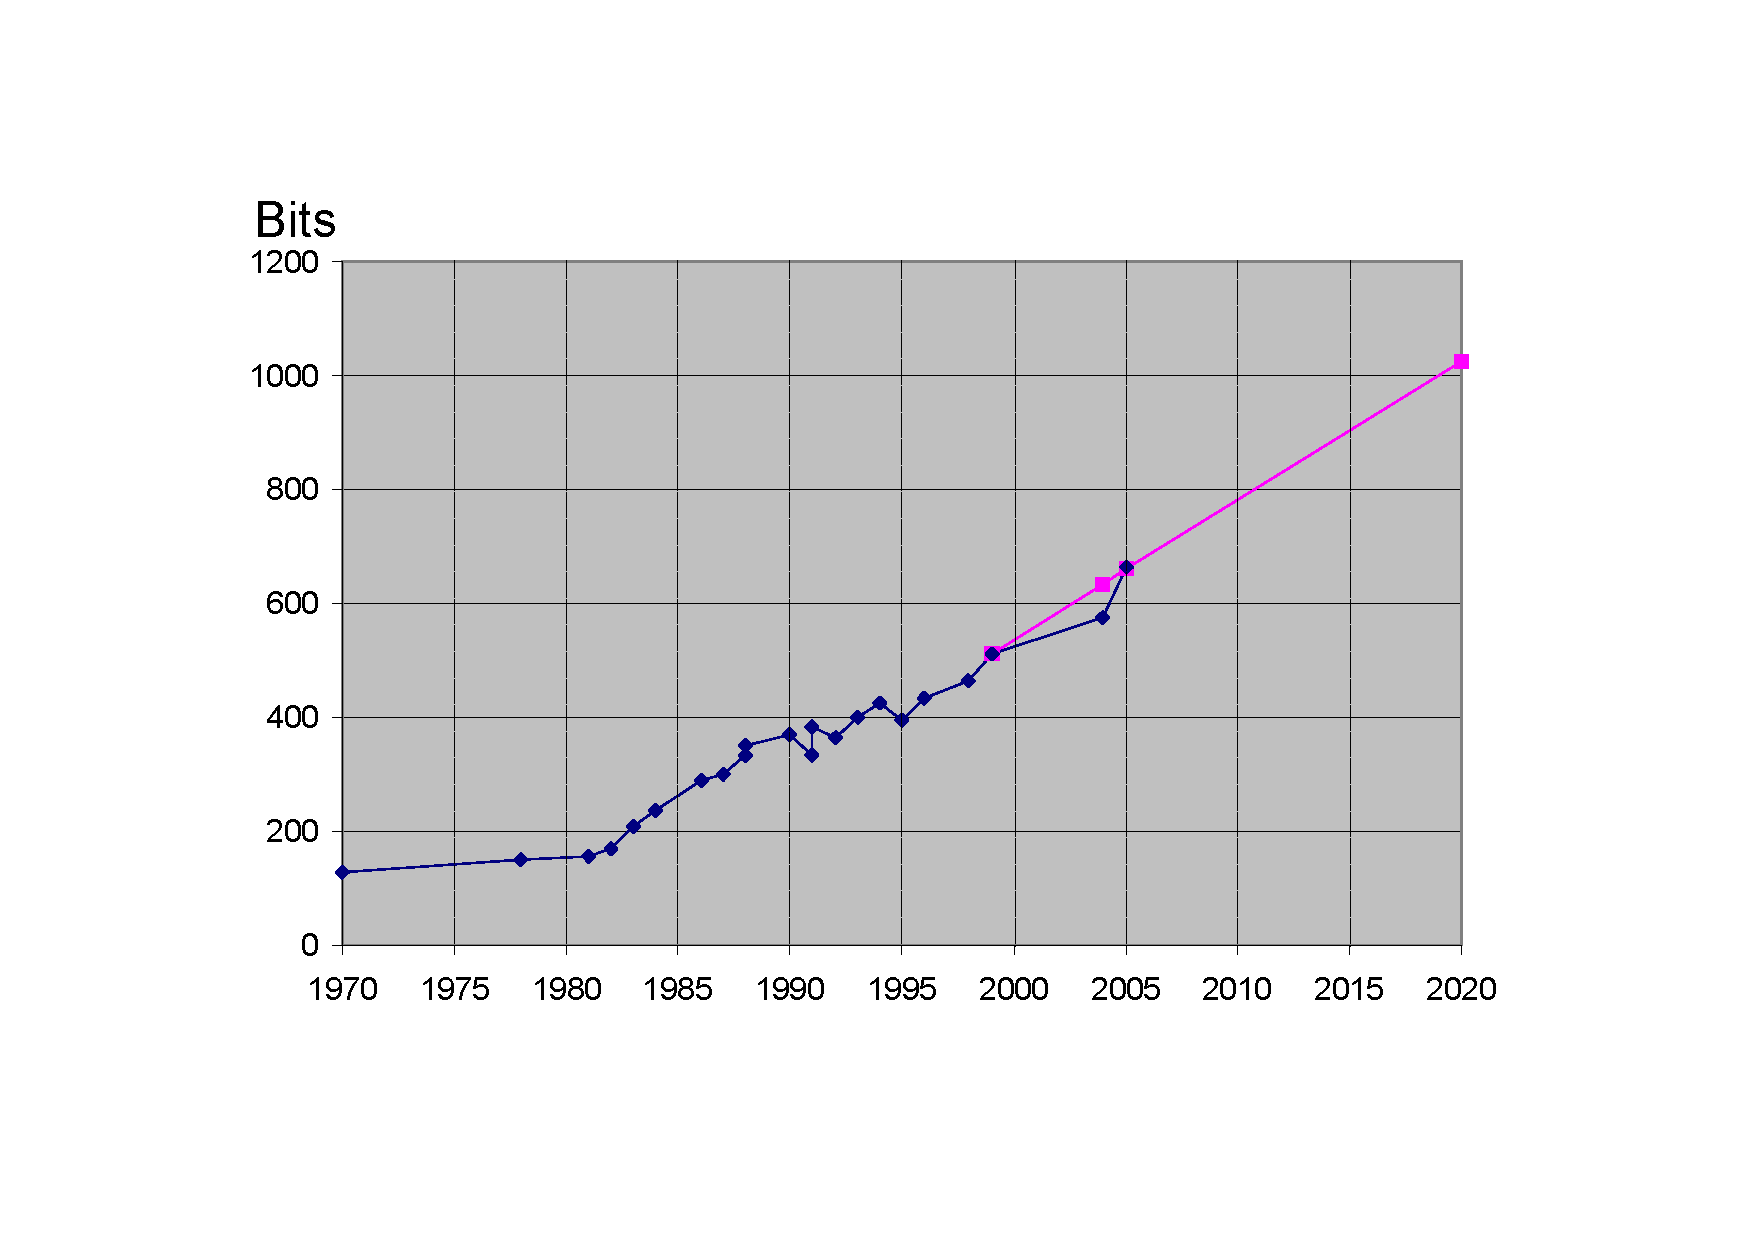
\includegraphics[scale=0.70, clip, viewport=50 20 700 430]{figures/PrognoseRSAFaktorisierungSecorvo.pdf}
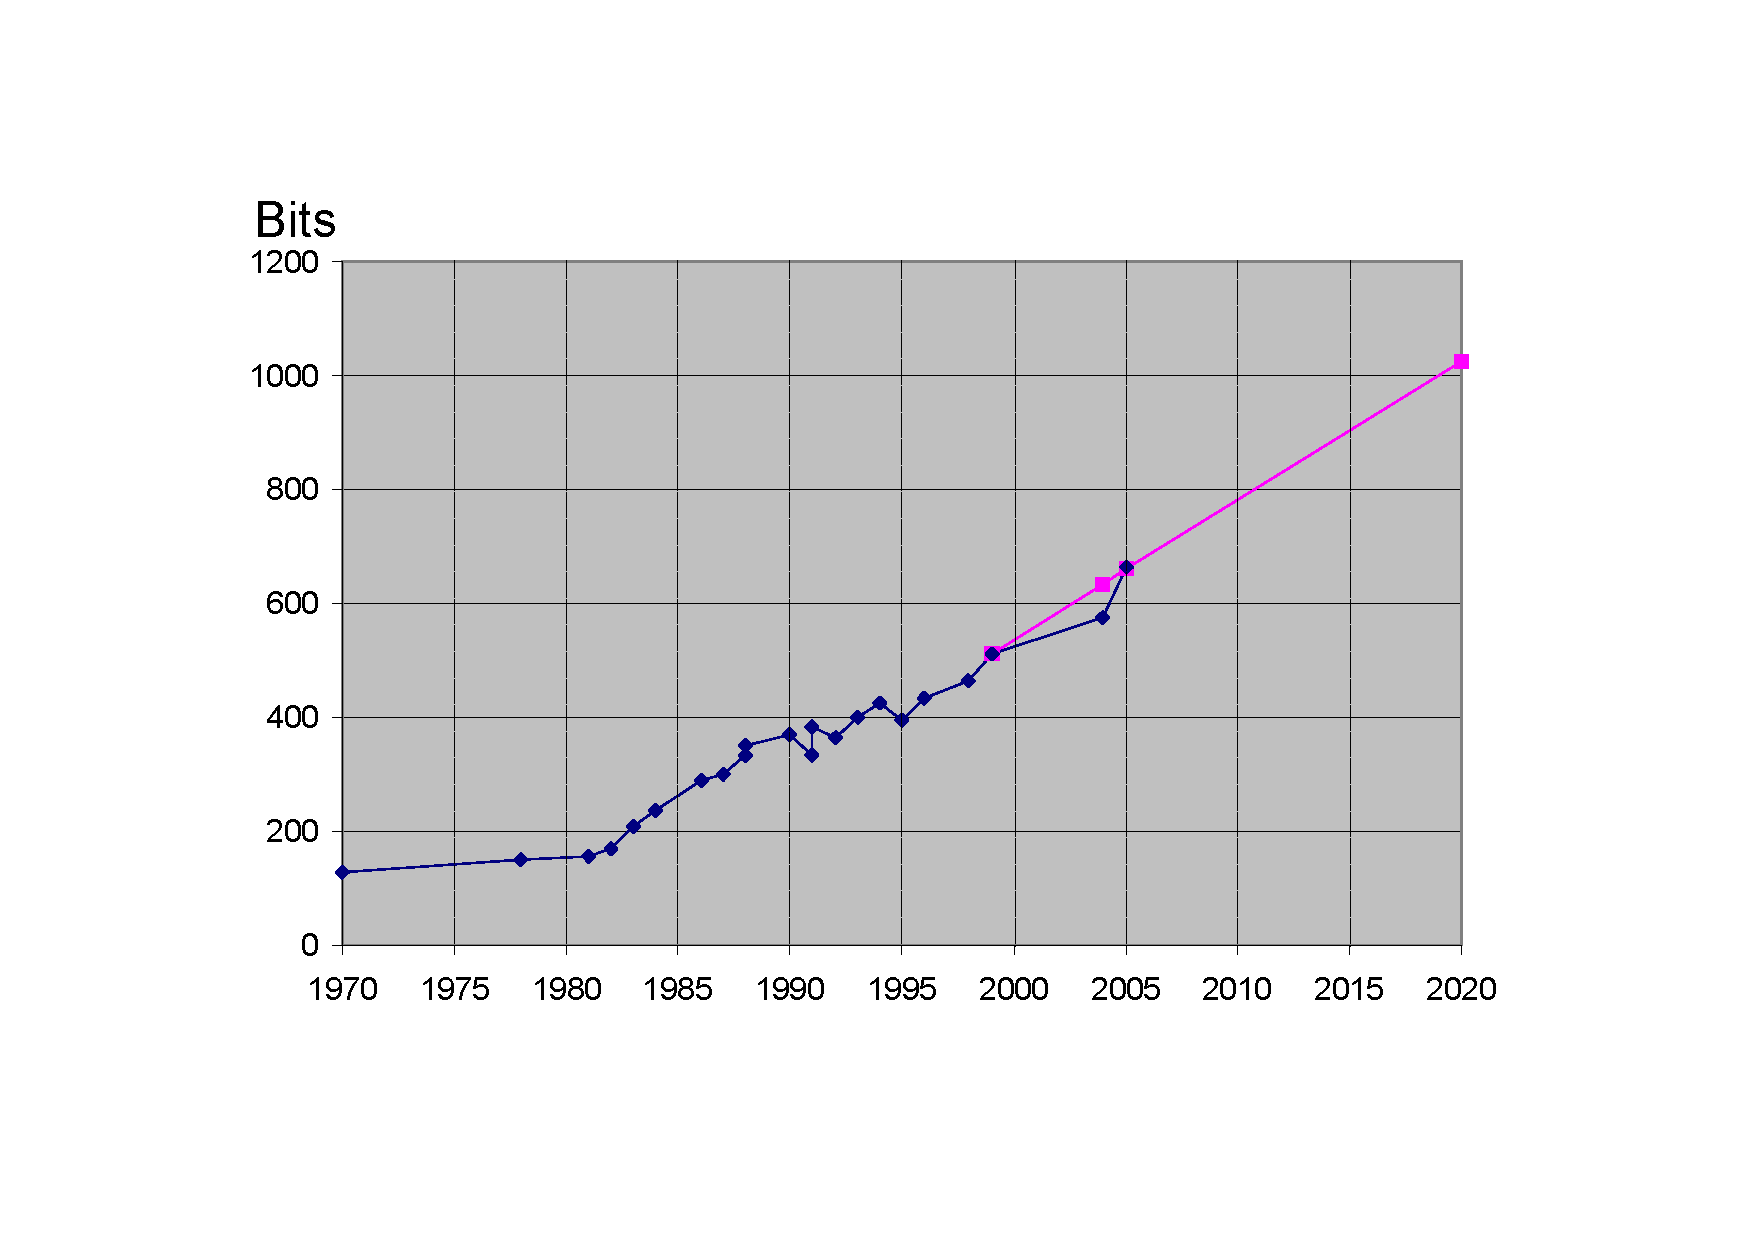
\includegraphics[scale=0.64, clip, viewport=-20 0 680 520]{figures/PrognoseRSAFaktorisierungSecorvo.pdf}
% Parameter von includegraphics: scale, x, y, dx, dy
% dx, dy spezifiziert die Ausdehnung, die man dem Bildes spendiert.
%      Ist dy zu klein, wird das Bild oben abgeschnitten
% x, y sagt, ab wo der Rahmen um das Bild gezeichnet wird.
%      Ist z.B. x=50, sind der linke Rahmenstrich und Teile des linken
%      Teiles des Bildes nicht zu sehen.
% scale dehnt Rahmenlinie und Bild aus -> Sitenrand wird bei 0.7 z.B. kleiner.
}
\caption{Vorhersage �ber die zuk�nftigen Faktorisierungsrekorde verglichen
mit aktuellen Resultaten (Quelle Secorvo)}
\label{secorvo-factorisation-forecast}
\end{center}
\end{figure}

H�lt die Prognose, dann ist die Faktorisierung eines RSA-Moduls der L�nge
1024 Bit in 15 Jahren zu erwarten.




\clearpage  % Erzwingt, dass alle Floating Objekte (z.B. Grafiken VORHER
            % geschrieben werden ! (sonst wurde Kapitel 4.11.4 begonnen,
            % und die Secorvo-Grafik auf er Folgeseite UNTER die Fussnote
            % geschoben. Au�erdem wahrscheinlich auch Zeilenumbruch,
            % egal, ob nach der Garfik noch Platz ist.
% ++++++++++++++++++++++++++++++++++++++++++++++++++++++++++++++++++++++++++
\vspace{6ex}
\begin{center}
\fbox{\parbox{15cm}{
    \emph{Hermann Hesse\footnotemark:}\\
    Damit das M�gliche entsteht, muss immer wieder das Unm�gliche 
    versucht werden.
}}
\end{center}
\addtocounter{footnote}{0}\footnotetext{%
    Hermann Hesse, deutsch-schweizerischer Schriftsteller und Nobelpreistr�ger, 
    02.07.1877$-$09.08.1962.}
% ++++++++++++++++++++++++++++++++++++++++++++++++++++++++++++++++++++++++++

\subsection{Status der Faktorisierung von konkreten gro�en Zahlen}
\label{NoteFactorisation}

Ausf�hrliche �bersichten �ber die Rekorde im Faktorisieren
zusammengesetzter Zahlen \index{Faktorisierung!Faktorisierungsrekorde}
mit unterschiedlichen Methoden finden sich auf den folgenden Webseiten:
\vspace{-10pt}
\begin{itemize}
\item[]
     \href{http://www.crypto-world.com}
  {\texttt{http://www.crypto-world.com}} \\
     \href{http://www.tutorgig.com/ed/RSA\_number}
  {\texttt{http://www.tutorgig.com/ed/RSA\_number}}  ~~ The RSA Factoring Challenge \\
%  {\texttt{http://www.tutorgig.com/ed/RSA\_number}}\footnote{%
%Diese Seite war Ende Mai 2005 nicht ganz auf dem aktuellen Stand: RSA-200 fehlte.}. \\
     \href{http://en.wikipedia.org/wiki/Integer_factorization_records}
  {\texttt{http://en.wikipedia.org/wiki/Integer\_factorization\_records}}
\end{itemize}

Der aktuelle Rekord (Stand Mai 2005) mit der GNFS-Methode (General Number
Field Sieve) \index{General Number Field Sieve (GNFS)} liegt in der Zerlegung
einer allgemeinen $200$-stelligen Dezimalzahl in ihre beiden Primfaktoren.

\vskip +10pt
Die letzten Rekorde\footnote{%
Die  "`RSA-Zahlen"' sind gro�e semiprime Zahlen (d.h. Zahlen, die genau aus
2 Primfaktoren bestehen)\index{Zahlen!semiprime}. Sie wurden von der Firma
RSA Security generiert und ver�ffentlicht, und sie bilden die "`RSA Factoring
Challenge"': In diesem Wettbewerb werden die Primfaktoren dieser Zahlen
gesucht.
Siehe \href{http://www.rsa.com/rsalabs/node.asp?id=2092}
   {\texttt{http://www.rsa.com/rsalabs/node.asp?id=2092}}.

In der ersten RSA-Factoring-Challenge wurden die Zahlen, von RSA-100 bis
RSA-500, gem�� der Anzahl ihrer Dezimalstellen benannt; die zweite
RSA-Factoring-Challenge benannte die Zahlen anhand der Anzahl ihrer
Bin�rstellen. Innerhalb des zweiten Wettbewerbs sind Geldpreise f�r die
erfolgreiche Faktorisierung von RSA576 bis RSA2048 ausgelobt (RSA576, RSA640
etc. in 64-er Schritten). 
Die Zahl RSA617 bildet eine Ausnahme, da sie vor der �nderung des 
Namensschemas erzeugt wurde.

Die Forscher um Prof. Jens Franke (von der Universit�t Bonn, dem BSI und dem
CWI) sind nicht auf die Geldpreise aus, sondern wollen die Grenzen der
Forschung ausdehnen. Dadurch werden Aussagen �ber notwendige Minimall�ngen
f�r sichere RSA-Moduli fundierter. 

Die "`C-Zahlen"' stammen aus dem Cunningham-Projekt:
\href{http://www.cerias.purdue.edu/homes/ssw/cun/}
     {\texttt{http://www.cerias.purdue.edu/homes/ssw/cun/}}
                                                               } 
mit Faktorisierungsverfahren f�r zusammengesetzte Zahlen
sind in der folgenden Tabelle~\ref{factorizationrecords} aufgef�hrt:

\begin{table}[ht]
\begin{center}
\begin{tabular}{|c|cccc|}
\hline
   & {\bf Dezimalstellen} & {\bf Bin�rstellen} & {\bf Faktorisiert am} & {\bf Faktorisiert von} \\
\hline
	C307 & 		307 & 1017 &  Mai, 2007 & Jens Franke et al. \\
	RSA-200 & 	200 & 663 & Mai, 2005 & Jens Franke et al. \\
	RSA640\footnotemark & 	193 & 600 & November, 2005 & Jens Franke et al. \\
	C176 & 		176 & 583 & Mai, 2005 & Kazumaro Aoki et al. \\
	RSA576 & 	174 & 576 & Dezember, 2003 & Jens Franke et al. \\
	RSA-160 & 	160 & 530 & April, 2003 & Jens Franke et al. \\
	C158 & 		158 & 523 & Januar, 2002 & Jens Franke et al. \\
	RSA-155	&	155 & 512 & August, 1999 & Herman te Riele et al. \\
\hline
\end{tabular}
\caption{Die derzeitigen Faktorisierungsrekorde (Stand Juli 2009)}    % Eyecatcher_neue-Mersenne
\label{factorizationrecords}
\end{center}
\end{table}
\footnotetext{%
Eine Arbeitsgruppe des BSI hat die mit 20.000 US-Dollar dotierte Challenge
RSA-640 mit Hilfe der GNFS-Methode gel�st. Die Forscher ben�tigten f�r die
Zerlegung der Zahl in ihre beiden 320 Bit langen Primfaktoren rund f�nf
Monate Rechenzeit.\\
Die RSA-Laboratorien schreiben ihre Challenges schon seit Anfang der
90er-Jahre aus. Die n�chst gr��ere Challenge ist nun die mit 30.000
US-Dollar dotierte RSA-704.\\
Siehe:
\href{http://www.heise.de/newsticker/meldung/print/65957}
{\texttt{http://www.heise.de/newsticker/meldung/print/65957}}
}
%be_2005: Erzwingen, dass die Abb. noch in diesem Kapitel !


Im Folgenden werden diese letzten Rekorde etwas ausf�hrlicher erl�utert.
Die beiden dabei benutzten Methoden GNFS und SNFS werden kurz z.B. auf
den ff. Webseiten dargestellt:
\index{General Number Field Sieve (GNFS)}
\index{Special Number Field Sieve (SNFS)}
\vspace{-10pt}
\begin{itemize}
\item[]
      \href{http://en.wikipedia.org/wiki/Special_number_field_sieve}
   {\texttt{http://en.wikipedia.org/wiki/Special\_number\_field\_sieve}} \\
      \href{http://en.wikipedia.org/wiki/General_number_field_sieve}
   {\texttt{http://en.wikipedia.org/wiki/General\_number\_field\_sieve}}
\end{itemize}
%\vspace{-10pt}


% --------------------------------------------------------------------------
\vskip +20pt
\paragraph{RSA-155} \label{RSA-155} \index{RSA-155} 
\mbox{} % f�r Zeilenumbruch, da er // allein nicht mag ! xxxxxxxxx

Am 22. August 1999 fanden niederl�ndische Forscher die L�sung dieser 
RSA-Challenge. Sie zerlegten eine $155$-stellige Zahl in ihre beiden $78$-stelligen
Primfaktoren (vergleiche Kapitel~\ref{chptSecurityParam}).
Mit der $512$ Bit-Zahl RSA-155 war eine {\em magische} Grenze erreicht.



% --------------------------------------------------------------------------
\vskip +20pt
\paragraph{C158} \label{C158} \index{C158} 
\mbox{} % f�r Zeilenumbruch, da er \\ allein nicht mag ! xxxxxxxxx
\hypertarget{C158-chap3}{}

Am 18. Januar 2002 zerlegten Forscher der Universit�t Bonn\footnote{%
\href{http://www.uni-bonn.de/Aktuelles/Pressemitteilungen/pm02/pm035-02.html}
{\texttt{http://www.uni-bonn.de/Aktuelles/Pressemitteilungen/pm02/pm035-02.html}}} 
mit der GNFS-Methode (General Number Field Sieve) \index{General Number
Field Sieve (GNFS)} eine $158$-stellige Dezimalzahl in ihre beiden Primfaktoren 
(diese haben 73 und 86 Dezimalstellen).

Dieser Rekord fand deutlich weniger Aufmerksamkeit in der Presse als die
L�sung von RSA-155.

Die Aufgabe der Bonner Wissenschaftler entsprang auch nicht einer Challenge,
sondern die Aufgabe war, die letzten Primfaktoren der Zahl $2^{953}+1$ 
zu finden (siehe~ ``Wanted List'' des Cunningham-Projekts\index{Cunningham-Projekt}%
\footnote{%
Cunningham-Projekt: \href{http://www.cerias.purdue.edu/homes/ssw/cun/}
                 {\texttt{http://www.cerias.purdue.edu/homes/ssw/cun/}}}). 

Die 6 kleineren, schon vorher gefundenen Primfaktoren dieser Zahl waren:
$$
\begin{array}{c}
        3, 1907, 425796183929, \\ 
        1624700279478894385598779655842584377, \\
        3802306738549441324432139091271828121 \quad{\rm und} \\ 
        128064886830166671444802576129115872060027.
\end{array}
$$
\begin{sloppypar}
Die drei kleinsten Faktoren k�nnen leicht\footnote{%
Z.B. mit CrypTool\index{CrypTool} �ber das Men� 
{\bf Einzelverfahren \textbackslash{} RSA-Kryptosystem \textbackslash{} 
Faktorisieren einer Zahl}. \\
In sinnvoller Zeit zerlegt CrypTool Zahlen bis 250 Bit L�nge.
Zahlen gr��er als 1024 Bit werden zur Zeit von CrypTool nicht angenommen.
}
bestimmt werden.
Die n�chsten drei Primfaktoren wurden von P.~Zimmerman%
\footnote{\href{http://www.loria.fr/zimmerma/ecmnet}{\tt http://www.loria.fr/\~{}zimmerma/ecmnet}}, 
T.~Grandlund%
\footnote{\href{http://www.swox.se/gmp/}{\tt http://www.swox.se/gmp/}}
und R. Harley in den Jahren 1999 und 2000 mit der Methode der Elliptischen
Kurven gefunden.
\end{sloppypar}

Als letzter Faktor blieb der sogenannte Teiler  "`C158"',
von dem man bis dahin wusste, dass er zusammengesetzt ist, aber man kannte
seine Primfaktoren nicht (die folgenden drei Zeilen sind eine einzige Zahl):
$$
\begin{array}{c}
39505874583265144526419767800614481996020776460304936 \\
45413937605157935562652945068360972784246821953509354 \\
4305870490251995655335710209799226484977949442955603
\end{array}
$$
Die Faktorisierung von C158 ergab die beiden 73- und 86-stelligen Primfaktoren:
$$
\begin{array}{c}
3388495837466721394368393204672181522815830368604993048084925840555281177
\end{array}
$$
und
$$
\begin{array}{c}
1165882340667125990314837655838327081813101 \\
2258146392600439520994131344334162924536139.
\end{array}
$$
Damit wurde die Zahl $2^{953}+1$ vollst�ndig in ihre 8 Primfaktoren zerlegt.

\noindent\begin{minipage}{\textwidth}
\vspace{3ex}
Verweise:
\vspace{-10pt}
\begin{itemize}
\item[]   \url{http://www.loria.fr/~zimmerma/records/gnfs158}\\
          \url{http://www.crypto-world.com/FactorRecords.html}\\
          \url{http://www.crypto-world.com/announcements/c158.txt}
\end{itemize}
\end{minipage}
\vspace{24pt}



% --------------------------------------------------------------------------
\vskip +20pt
\paragraph{RSA-160} \label{RSA-160} \index{RSA-160}\mbox{}
\hypertarget{RSA-160-chap3}{}

Am 1. April 2003 zerlegten Forscher der Universit�t Bonn\footnote{%
          \href{http://www.loria.fr/~zimmerma/records/rsa160}
       {\texttt{http://www.loria.fr/\~{}zimmerma/records/rsa160}} \\
          \href{http://www.loria.fr/~zimmerma/records/factor.html}
       {\texttt{http://www.loria.fr/\~{}zimmerma/records/factor.html}} \\
          \href{http://www.crypto-world.com/FactorWorld.html}
       {\texttt{http://www.crypto-world.com/FactorWorld.html}}
} 
mit der GNFS-Methode (General Number Field Sieve) \index{General Number
Field Sieve (GNFS)} eine $160$-stellige Zahl in ihre beiden Primfaktoren 
(diese haben jeweils 80 Dezimalstellen).

Die Berechnungen dazu fanden auch im Bundesamt f�r Sicherheit in der 
Informationstechnik (BSI) in Bonn statt\footnote{%
Das BSI \index{BSI} erstellt jedes Jahr ein Papier �ber die Eignung von
Kryptoalgorithmen, mit denen Signaturen erzeugt werden k�nnen,         
die den Vorgaben des deutschen Signaturgesetzes gen�gen.
Bei dieser Erstellung werden Experten aus Wirtschaft und Wissenschaft
beteiligt. Um die Eignung von Signaturverfahren zu beurteilen, deren
Schwierigkeit auf dem Faktorisierungsproblem beruht,
kooperiert das BSI auch mit Forschern der Universit�t Bonn.
Weitere Informationen zu Kryptoalgorithmen finden Sie auf den BSI-Internetseiten unter:
   \href{http://www.bsi.bund.de/esig/basics/techbas/krypto/index.htm}
{\texttt{http://www.bsi.bund.de/esig/basics/techbas/krypto/index.htm}}
}.

Die 160-stellige Dezimalzahl stammt von der alten Challenge-Liste von RSADSI.
Diese wurde nach der Faktorisierung von RSA-155 (RSA512) zur�ckgezogen.
Die Primfaktoren von RSA-160 waren aber nicht bekannt.
Deshalb ist dieser Rekord von Prof.\ Frankes Team immer noch die L�sung 
einer alten Challenge, f�r die es aber von RSADSI kein Geld gibt.

Die zusammengesetzte Zahl "`RSA-160"' lautet (die folgenden drei Zeilen 
sind eine einzige Zahl):
$$
\begin{array}{c}
215274110271888970189601520131282542925777358884567598017049 \\
767677813314521885913567301105977349105960249790711158521430 \\
2079314665202840140619946994927570407753
\end{array}
$$
Die Faktorisierung von RSA-160 ergab die beiden Primfaktoren:
$$
\begin{array}{c}
p = 45427892858481394071686190649738831 \\         
    656137145778469793250959984709250004157335359
\end{array}
$$
und
$$
\begin{array}{c}
q = 47388090603832016196633832303788951 \\
    973268922921040957944741354648812028493909367
\end{array}
$$

Die Berechnungen erfolgten zwischen Dezember 2002 und April 2003.
\vspace{24pt}



% ammmmmmmmmmma
% 
% RSA-576 faktorisiert 
% Am 27.04.2004 ging die Nachricht durch
% die Ticker, dass die 576-bit-Challenge der
% Firma RSA gel�st sei. Tats�chlich wurde
% die 174 Dezimalstellen lange Zahl bereits
% am 03.12.2003 zerlegt. Die Faktorisierung
% gelang einem Team der Universit�t Bonn
% um Professor Franke mit Unterst�tzung
% durch das Institut f�r Experimentelle Mathematik
% in Essen und das BSI. Die verteilte
% Berechung erfolge auf einem Linux-
% Cluster mit 144 PCs (400 MHz, Pentium II)
% und verwendete den General Number Field
% Sieve-Algorithmus ? mit einem Aufwand
% von umgerechnet 13.200 MIPS-Jahren.
% Interessant dabei: Dieser Faktorisierungserfolg
% best�tigt die Prognose, die Secorvo
% vor drei Jahren auf der Basis der Faktorisierungserfolge
% der vergangenen 30 Jahre
% gestellt hat (siehe Bild), und die weit weniger
% dramatisch ausfiel als viele Expertenwarnungen
% und die Erwartung des BSI.
% Danach w�re 2004 erstmals die Faktorisierung
% einer 630 bit langen Zahl zu erwarten
% gewesen ? was nun eher unwahrscheinlich
% erscheint. Selbst die fr�hestens f�r das
% Jahr 2020 vorausgesagte Faktorisierung
% eines 1024 bit langen RSA-Schl�ssels
% k�nnte sich daher noch als zu pessimistische
% Bef�rchtung erweisen ? allen Warnern
% zum Trotz, die seit Jahren Schl�ssell
% �ngen von 2048 bit und mehr empfehlen
% oder gar das baldige Ende von RSA prophezeihen.
% 
% ammmmmmmmmmmz




% --------------------------------------------------------------------------
\vskip +20pt
\hypertarget{RSA-200-chap3}{}
\paragraph{RSA-200} \label{RSA-200} \index{RSA-200}\mbox{}
\nopagebreak

Am 9. Mai 2005 meldete die Forschergruppe von Prof. Jens Franke der Universit�t Bonn\footnote{%
   \href{http://www.loria.fr/~zimmerma/records/rsa200}
{\texttt{http://www.loria.fr/\~{}zimmerma/records/rsa200}}}, dass sie
gemeinsam mit Kollegen des Amsterdam Centrum voor Wiskunde en Informatica
einen neuen Weltrekord im Faktorisieren aufstellten. 

Sie zerlegten mit der GNFS-Methode (General Number Field Sieve) \index{General Number
Field Sieve (GNFS)} eine $200$-stellige Zahl in ihre beiden Primfaktoren 
(diese haben jeweils 100 Dezimalstellen).

Die zusammengesetzte Zahl "`RSA-200"' lautet (die folgenden drei Zeilen 
sind eine einzige Zahl):
$$
\begin{array}{c}
2799783391122132787082946763872260162107044678695542853756000992932 \\
6128400107609345671052955360856061822351910951365788637105954482006 \\
576775098580557613579098734950144178863178946295187237869221823983
\end{array}
$$
Die Faktorisierung von RSA-200 ergab die beiden Primfaktoren:
$$
\begin{array}{c}
p = 35324619344027701212726049781984643686711974001976 \\
    25023649303468776121253679423200058547956528088349
\end{array}
$$
und
$$
\begin{array}{c}
q = 79258699544783330333470858414800596877379758573642 \\
    19960734330341455767872818152135381409304740185467
\end{array}
$$

Die Berechnungen erfolgten zwischen Dezember 2003 und Mai 2005.
Die Faktorisierung durch die Gruppe um Bahr, B�hm, Franke, Kleinjung, 
Montgomery und te Riele hatte also knapp 17 Monate gedauert.
Der Rechenaufwand lag bei umgerechnet etwa 120.000 MIPS-Jahren\footnote{%
Ein MIPS-Jahr (MY) ist die Anzahl von Operationen, die eine Maschine, 
welche eine Million Integeroperationen pro Sekunde (MIPS)
ausf�hrt, in einem Jahr bew�ltigt. Zur Illustration: ein INTEL 
Pentium 100 Prozessor hat etwa 50 MIPS.
F�r die Zerlegung eines 2048-Bit-Moduls br�uchte man ca. {$8,5 \cdot 
10^{40}$ MY}.}.
\vspace{24pt}





% --------------------------------------------------------------------------
\vskip +20pt
\paragraph{C307 / M1039} \label{C307} \index{C307} \index{M1039} 
\mbox{} % f�r Zeilenumbruch, da er \\ allein nicht mag ! xxxxxxxxx
\hypertarget{C307-chap3}{}

Im Mai 2007 meldeten Prof. Franke, Prof. Kleinjung (von der Universit�t Bonn),
das japanische Telekommunikationsunternehmen NTT und Prof. Arjen Lenstra von
der Polytechnischen Hochschule in Lausanne, dass sie mit der SNFS-Methode
(Special Number Field Sieve) \index{Special Number Field Sieve (SNFS)}
innerhalb von 11 Monaten
eine $307$-stellige Dezimalzahl in ihre beiden Primfaktoren zerlegten
(diese haben 80 und 227 Dezimalstellen).

Die Aufgabe der Wissenschaftler entsprang nicht einer Challenge, sondern
die Aufgabe war, die letzten Primfaktoren der Mersenne-Zahl $2^{1039}+1$ 
zu finden (siehe~ \glqq Wanted List\grqq~ des Cunningham-Projekts\index{Cunningham-Projekt}%
\footnote{%
Cunningham-Projekt: \href{http://www.cerias.purdue.edu/homes/ssw/cun/}
                 {\texttt{http://www.cerias.purdue.edu/homes/ssw/cun/}}\\
Cunningham-Tabelle: \href{http://homes.cerias.purdue.edu/~ssw/cun/pmain1206}
                 {\texttt{http://homes.cerias.purdue.edu/\~{}ssw/cun/pmain1206}}\\
Die Zahlen in der Cunningham-Tabelle werden folgenderma�en geschrieben:\\
\glqq (2,n)-\grqq~ bedeutet $2^{n}-1$;~~~
\glqq (2,n)+\grqq~ bedeutet $2^{n}+1$.\\
Um die Gr��enordnung einer Zerlegung anzudeuten schreibt man $p<n>$ oder $c<n>$,
wobei \glqq n\grqq~ die Anzahl der Dezimalstellen ist und \glqq p\grqq~ und \glqq c\grqq~
bedeuten, dass die Zahl eine Primzahl oder eine zusammengesetzte Zahl ist.\\
$2^{1039}-1 = p7 * c307 = p7 * p80 * p227$ \\
Genauer erkl�rt wird dies auf der CUN-Seite folgenderma�en:\\
\glqq 2,651+ means $2^{651} + 1$ and the size (c209 means 209 decimal digits)
of the
number which was factored.  Then come the new factor(s), the discoverer and
the method used.  Recently, only the multiple polynomial quadratic sieve
(ppmpqs), the elliptic curve method (ecm) and the number field sieve (nfs)
have been used.  `hmpqs' stands for hypercube multiple polynomial quadratic
sieve.  Under `new factors', `p90' means a 90-digit prime and `c201' is a
201-digit composite number.\grqq. 
}).\\


Die Zahl $2^{1039}-1$ besteht aus 3 Primfaktoren: Der kleinste Faktor
$p7 = 5080711$ war schon l�nger bekannt.\footnote{%
Er kann mit CrypTool\index{CrypTool} �ber das Men� 
{\bf Einzelverfahren \textbackslash{} RSA-Kryptosystem \textbackslash{} 
Faktorisieren einer Zahl} gefunden werden --- mit den Algorithmen von Brent,
Williams oder Lenstra, mit denen man gut \glqq relativ\grqq~ kleine Faktoren
abspalten kann. \\
In sinnvoller Zeit zerlegt CrypTool vollst�ndig Zahlen bis 250 Bit L�nge.
}

Zur vollst�ndigen Faktorisierung musste der zweite Faktor (Koteiler) "`C307"'
zerlegt werden: Bis dahin wusste man nur, dass er zusammengesetzt ist, aber man
kannte weder die Anzahl seiner Primfaktoren, noch die Primfaktoren selbst.
Die folgenden f�nf Zeilen sind eine einzige Zahl:
$$
\begin{array}{c}
C307 =1159420574072573064369807148876894640753899791702017724986868353538\\
8224838599667566080006095408005179472053993261230204874402860435302\\
8619141014409345351233471273967988850226307575280937916602855510550\\
0425810771176177610094137970787973806187008437777186828680889844712\\
822002935201806074755451541370711023817
\end{array}
$$
Die Faktorisierung von C307 ergab die beiden 80- und 227-stelligen Primfaktoren:
$$
\begin{array}{c}
p80 = 558536666199362912607492046583159449686465270184\\
      88637648010052346319853288374753
\end{array}
$$
und
$$
\begin{array}{c}
p227 = 207581819464423827645704813703594695162939708007395209881208\\
       387037927290903246793823431438841448348825340533447691122230\\
       281583276965253760914101891052419938993341097116243589620659\\
       72167481161749004803659735573409253205425523689
.
\end{array}
$$
Damit wurde die Zahl $2^{1039}-1$ vollst�ndig in ihre 3 Primfaktoren zerlegt.

\noindent\begin{minipage}{\textwidth}
\vspace{3ex}
Verweise:
\vspace{-10pt}
\begin{itemize}
\item[]   \url{http://www.loria.fr/~zimmerma/records/21039-}\\
          \url{http://www.crypto-world.com/announcements/m1039.txt}\\
          \url{http://www.crypto-world.com/FactorAnnouncements.html}\\
          \url{http://www1.uni-bonn.de/pressDB/jsp/pressemitteilungsdetails.jsp?detailjahr=2007&detail=160}
\end{itemize}
\end{minipage}






% --------------------------------------------------------------------------
\vskip +50pt
\paragraph{Gr��enordnung faktorisierter Zahlen im Vergleich zu auf Primalit�t getesteter Zahlen}
\mbox{}

Wie man sieht, sind die gr��ten (aus 2 Primfaktoren) zusammengesetzten
Zahlen, die man faktorisieren kann, deutlich kleiner als die Zahlen mit
einer speziellen Struktur, f�r die Primzahltests\index{Primzahltest} in
der Lage sind, Aussagen �ber ihre Primalit�t zu treffen (siehe Kapitel 
\ref{search_for_very_big_primes},~\ref{primality_tests} und
\ref{spezialzahlentypen}).


% be_2005_UPDATEN_if-new-mersenne-prime-appears   % Eyecatcher_neue-Mersenne
L�nge in Bit der derzeitigen Weltrekorde:\\
$$  ~~~~~~~~~[RSA{-}200{-}Zahl] ~~\longleftrightarrow{}~~[43.~bekannte~Mersenne~Primzahl] $$
$$ 663 ~~ \longleftrightarrow{} ~~ 30.402.457 ~~~~~$$


%be_2005 - erzwungenes Blank und $$ um Pfeilzeichen, sonst setzt er Blanks an 
%          die falschen Stellen.
%        - Wenn man hier \~ statt nur ~ (au�erhalb der $$) schreibt, kommen
%          nachher Fussnoten mit 
%          {\bf Einzelverfahren \textbackslash{} Protokolle}
%          nur noch mit kaputten Schriftzeichen raus !



% --------------------------------------------------------------------------
\vskip +60pt
\subsection{Weitere aktuelle Forschungsergebnisse zu Primzahlen und Faktorisierung}
\label{FactorisationResearch}
Primzahlen sind Teil vieler hochaktueller Forschungsgebiete der Zahlentheorie. 
Die Fortschritte bei der Faktorisierung sind gr�� als noch vor 5 Jahren
gesch�tzt -- sie gehen nicht nur auf das Konto schnellerer Rechner, 
sondern sie sind auch in neuen Erkenntnissen begr�ndet.

Die Sicherheit des RSA-Algorithmus basiert auf der empirischen Beobachtung, dass die Faktorisierung gro�er ganzer 
Zahlen ein schwieriges Problem ist. Besteht wie beim RSA-Algorithmus der zugrunde liegende Modul $n$ aus dem Produkt 
zweier gro�er Primzahlen $p, q$ (typische L�ngen: $p, q$  $500-600$ bit, $n$ $1024$ bit), so l�sst sich 
$n=pq$ aus $p$ und $q$ leicht bestimmen, jedoch ist es mit den bisher bekannten Faktorisierungsalgorithmen nicht
m�glich, $p, q$ aus $n$ zu gewinnen. Nur mit Kenntnis von $p$ und $q$ l�sst sich jedoch der private aus dem 
�ffentlichen Schl�ssel ermitteln.

Die Entdeckung eines Algorithmus zur effizienten Faktorisierung von Produkten $n=pq$ gro�er Primzahlen w�rde daher 
den RSA-Algorithmus wesentlich beeintr�chtigen. Je nach Effizienz der Faktorisierung im Vergleich zur Erzeugung von 
$p, q, n$ m�sste der verwendete Modul $n$ (z.Zt. 1024 bit) erheblich vergr��ert oder --- im Extremfall --- auf den 
Einsatz des RSA ganz verzichtet werden.


% --------------------------------------------------------------------------
\vskip +20pt
\paragraph{Das Papier von Bernstein und seine Auswirkungen auf die Sicherheit
des RSA-Algorithmus} \label{RSABernstein} \index{Faktorisierung!Faktorisierungsproblem}
\mbox{} % f�r Zeilenumbruch, da er \\ allein nicht mag ! 
        % Braucht die Leerzeile danach auch noch !! bebebe ?

Die im November 2001 ver�ffentlichte Arbeit ``Circuits for integer
factorization: a proposal'' (siehe
\href{http://cr.yp.to/djb.html}{\texttt{http://cr.yp.to/djb.html}}) von
D.J. Bernstein \cite{nt:Bernstein2001} behandelt das Problem der 
Faktorisierung gro�er Zahlen.
Die Kernaussage des Papers besteht darin, dass es m�glich ist, die
Implementierung des General Number Field Sieve-Algorithmus (GNFS)
\index{General Number Field Sieve (GNFS)} so zu
verbessern, dass mit gleichem Aufwand wie bisher Zahlen mit 3-mal
gr��erer Stellenzahl (Bit-L�nge) faktorisiert werden k�nnen.

Wesentlich bei der Interpretation des Resultats ist die Definition des
Aufwandes: Als Aufwand wird das Produkt von ben�tigter Rechenzeit und
Kosten der Maschine (insbesondere des verwendeten Speicherplatzes)
angesetzt. Zentral f�r das Ergebnis des Papiers ist die Beobachtung, dass
ein wesentlicher Teil der Faktorisierung auf Sortierung zur�ckgef�hrt
werden kann und mit dem Schimmlerschen Sortierschema ein Algorithmus zur
Verf�gung steht, der sich besonders gut f�r den Einsatz von
Parallelrechnern eignet. Am Ende des Abschnittes 3 gibt Bernstein konkret
an, dass die Verwendung von $m^2$ Parallelrechnern mit jeweils gleicher
Menge an Speicherplatz mit Kosten in der Gr��enordnung von $m^2$
einhergeht --- genau so wie ein einzelner Rechner mit $m^2$ Speicherzellen.
Der Parallelrechner bew�ltigt die Sortierung von $m^2$ Zahlen jedoch
(unter Verwendung der o.~g.\ Sortierverfahrens) in Zeit proportional zu m,
wohingegen der Einprozessorrechner Zeit proportional $m^2$ ben�tigt.
Verringert man daher den verwendeten Speicherplatz und erh�ht --- bei
insgesamt gleich bleibenden Kosten --- die Anzahl der Prozessoren
entsprechend, verringert sich die ben�tigte Zeit um die Gr��enordnung
$1/m$. In Abschnitt 5 wird ferner angef�hrt, dass der massive Einsatz der
parallelisierten Elliptic Curve-Methode von Lenstra die Kosten der
Faktorisierung ebenfalls um eine Gr��enordnung verringert (ein
Suchalgorithmus hat dann quadratische statt kubische Kosten).  Alle
Ergebnisse von Bernstein gelten nur asymptotisch f�r gro�e Zahlen $n$.
Leider liegen keine Absch�tzungen �ber den Fehlerterm, d.h.  die
Abweichung der tats�chlichen Zeit von dem asymptotischen Wert, vor --- ein
Mangel, den auch Bernstein in seinem Papier erw�hnt. Daher kann zur Zeit
keine Aussage getroffen werden, ob die Kosten (im Sinne der Bernsteinschen
Definition) bei der Faktorisierung z.~Zt.\ verwendeter RSA-Zahlen
(1024$-$2048 bit) bereits signifikant sinken w�rden.

Zusammenfassend l�sst sich sagen, dass der Ansatz von Bernstein durchaus 
innovativ ist. Da die Verbesserung der 
Rechenzeit unter gleichbleibenden Kosten durch einen massiven Einsatz von 
Parallelrechnern erkauft wird, stellt sich die 
Frage nach der praktischen Relevanz. Auch wenn formal der Einsatz von einem 
Rechner �ber 1 sec  und  1.000.000 Rechnern 
f�r je 1/1.000.000 sec dieselben Kosten erzeugen mag, ist die 
Parallelschaltung von 1.000.000 Rechnern praktisch nicht 
(oder nur unter immensen Fixkosten, insbesondere f�r die Vernetzung der
Prozessoren) zu realisieren. Solche Fixkosten 
werden aber nicht in Ansatz gebracht.
Die Verwendung verteilter Ans�tze (distributed computing) �ber ein 
gro�es Netzwerk k�nnte einen Ausweg bieten. Auch hier m�ssten  
Zeiten und Kosten f�r Daten�bertragung einkalkuliert werden.

Solange noch keine (kosteng�nstige) Hardware oder verteilte Ans�tze 
entwickelt wurden, die auf 
dem Bernsteinschen Prinzip basieren, besteht noch keine akute Gef�hrdung
des RSA. Es bleibt zu kl�ren, ab welchen 
Gr��enordnungen von n die Asymptotik greift. 

Arjen Lenstra, Adi Shamir et.~al.\ haben das Bernstein-Paper analysiert 
\cite{nt:Lenstra2002}.
Als Ergebnis kommen Sie zu einer Bitl�ngen-Verbesserung der 
Faktorisierung um den Faktor 1.17 
(anstatt Faktor 3 wie von Bernstein erwartet).

Die Zusammenfassung ihres Papers ``Analysis of Bernstein's Factorization 
Circuit'' lautet:

``... Bernstein proposed a circuit-based implementation of
the matrix step of the number field sieve factorization algorithm. We
show that under the non-standard cost function used in [1], these circuits
indeed offer an asymptotic improvement over other methods but
to a lesser degree than previously claimed: for a given cost, the new
method can factor integers that are 1.17 times larger (rather than 3.01).
We also propose an improved circuit design based on a new mesh routing
algorithm, and show that for factorization of 1024-bit integers the
matrix step can, under an optimistic assumption about the matrix size,
be completed within a day by a device that costs a few thousand dollars.
We conclude that from a practical standpoint, the security of RSA relies
exclusively on the hardness of the relation collection step of the number
field sieve.''

Auch \href{http://www.rsasecurity.com/}{RSA Security} kommt in ihrer Analyse der Bernstein-Arbeit \cite{nt:RSA Security 2002} vom 8. April 2002 erwartungsgem��
zu dem Ergebnis, dass RSA weiterhin als ungebrochen betrachtet werden kann.

Die Diskussion ist weiterhin im Gang.

Zum Zeitpunkt der Erstellung dieses Absatzes (Juni 2002) war nichts
dar�ber bekannt, inwieweit die im Bernstein-Papier vorgeschlagenen
theoretischen Ans�tze realisiert wurden oder wieweit die Finanzierung
seines Forschungsprojektes ist.

\noindent\begin{minipage}{\textwidth}
\vspace{3ex}
Verweise:
\vspace{-10pt}
\begin{itemize}
  \item[] \href{http://cr.yp.to/djb.html}
               {\texttt{http://cr.yp.to/djb.html}} \\
          \href{http://www.counterpane.com/crypto-gram-0203.html\#6}
               {\texttt{http://www.counterpane.com/crypto-gram-0203.html\#6}} \\
          \href{http://www.math.uic.edu}
               {\texttt{http://www.math.uic.edu}} 
\end{itemize}
\end{minipage}



% --------------------------------------------------------------------------
\vskip +20pt
\paragraph{Das TWIRL-Device} \label{TWIRLDevice} \index{TWIRL-Device}
\mbox{} % f�r Zeilenumbruch, da er // allein nicht mag ! xxxxxxxxx

Im Januar 2003 ver�ffentlichten Adi Shamir und Eran Tromer vom Weizmann
Institute of Science den vorl�ufigen Draft {\em ``Factoring Large Numbers
with the TWIRL Device''}, in dem deutliche Bedenken gegen RSA-Schl�ssell�ngen
unter 1024 begr�ndet werden \cite{nt:Shamir2003}.

Das Abstract fasst ihre Ergebnisse folgenderma�en zusammen: ``The security of the RSA cryptosystem depends on the difficulty of factoring large integers. The best current factoring algorithm is the Number Field Sieve (NFS), and its most difficult part is the sieving step. In 1999 a large distributed computation involving thousands of workstations working for many months managed to factor a 512-bit RSA key, but 1024-bit keys were believed to be safe for the next 15-20 years. In this paper we describe a new hardware implementation of the NFS sieving step ... which is 3-4 orders of magnitude more cost effective than the best previously published designs ... . Based on a detailed analysis of all the critical components (but without an actual implementation), we believe that the NFS sieving step for 1024-bit RSA keys can be completed in less than a year by a \$10M device, and that the NFS sieving step for 512-bit RSA keys can be completed in less than ten minutes by a \$10K device. Coupled with recent results about the difficulty of the NFS matrix step ... this raises some concerns about the security of these key sizes.''

Eine ausf�hrliche Fassung findet sich auch in dem Artikel der beiden Autoren
in den RSA Laboratories CryptoBytes \cite{nt:Shamir2003a}.

Eine sehr gute Erl�uterung, wie der Angriff mit dem Generalized Number Field
Sieve (GNFS) \index{General Number Field Sieve (GNFS)} funktioniert und
welche Fortschritte sich ergaben, findet sich
in dem 3-seitigen Artikel in der DuD-Ausgabe Juni/2003 \cite{nt:Weis2003}.
Beim GNFS k�nnen 2 grundlegende Schritte unterschieden werden: 
der Siebungsschritt (Relationen sammeln) und die Matrix-Reduktion.
Auch wenn der Siebungsschritt hochgradig parallelisierbar ist, so dominiert
er doch den Gesamtrechenaufwand. Bisher haben Shamir und Tromer noch kein 
TWIRL-Device gebaut, jedoch ist der daf�r gesch�tzte Aufwand von 10 bis
50 Millionen Euro, um eine 1024-Bit Zahl in einem Jahr zu faktorisieren
f�r Geheimdienste oder gro�e kriminelle Organisationen keineswegs prohibitiv,
denn die \glqq Kosten f�r einen einzigen Spionagesatelliten sch�tzt man
z.B. auf mehrere Milliarden USD\grqq. Die Autoren empfehlen deshalb konkret,
m�glichst rasch sensible, bisher benutzte RSA-, Diffie-Hellman- oder 
ElGamal-Schl�ssel von bis zu 1024 Bit zu wechseln und Schl�ssel von 
mindestens 2048 Bit L�nge einzusetzen.
Auch f�r die geplante TCPA/Palladium-Hardware \index{Palladium} werden
2048-Bit RSA-Schl�ssel verwendet!

Damit erscheinen die aktuellen Empfehlungen des BSI, auf l�ngere 
RSA-Schl�ssell�ngen umzustellen, mehr als gerechtfertigt.



% --------------------------------------------------------------------------
\vskip +20pt
%\paragraph{``Primes in P'': Testen auf Primalit�t ist polynominal}
\paragraph{\glqq Primes in P\grqq: Testen auf Primalit�t ist polynominal}
\label{PrimesinP} \index{Primzahltest} 
\mbox{} % f�r Zeilenumbruch, da er // allein nicht mag ! xxxxxxxxx

Im August 2002 ver�ffentlichten die drei indischen Forscher M. Agrawal, 
N. Kayal und N. Saxena ihr Paper {\em \glqq PRIMES in P\grqq}  %{\em ``PRIMES in P''} 
�ber einen neuen Primzahltest-Algorithmus, genannt AKS\index{AKS} \cite{nt:Agrawal2002}.
Sie entdeckten einen polynominalen\index{Polynom} deterministischen Algorithmus, um zu entscheiden, ob eine gegebene Zahl prim ist oder nicht.

Die Bedeutung dieser Entdeckung liegt darin, dass sie Zahlentheoretiker mit neuen Einsichten und M�glichkeiten f�r die weitere Forschung versorgt. Viele Menschen haben im Lauf der Jahrhunderte nach einem polynominalen Primzahltest gesucht, so dass dieses Ergebnis einen theoretischen Durchbruch darstellt. Es zeigt sich immer wieder, dass aus schon lange bekannten Fakten neue Ergebnisse generiert werden k�nnen.

Aber selbst die Autoren merken an, dass andere bekannte Algorithmen (z.B. ECPP) schneller sein k�nnen. Der neue Algorithmus funktioniert f�r alle positiven ganzen Zahlen. Dagegen verwendet das GIMPS-Projekt den Lucas-Lehmer-Primzahltest, der besondere Eigenschaften der Mersennezahlen ausnutzt. Dadurch ist der Lucas-Lehmer-Test viel schneller und erlaubt, Zahlen mit Millionen von Stellen zu testen, w�hrend generische Algorithmen auf Zahlen mit einigen tausend Stellen beschr�nkt sind. Nachteil der bisherigen schnellen Verfahren ist, dass sie probabilistisch sind, also ihr Ergebnis h�chstwahrscheinlich, aber nicht ganz sicher ist.

\enlargethispage{20pt}
\noindent Aktuelle Forschungsergebnisse dazu finden sich z.B. auf: 
\vspace{-10pt}
\begin{itemize}
  \item[] \href{http://www.mersenne.org/}
               {\texttt{http://www.mersenne.org/}} \\
          \href{http://fatphil.org/maths/AKS/}
               {\texttt{http://fatphil.org/maths/AKS/}} Originaltext in Englisch\\
          \href{http://ls2-www.cs.uni-dortmund.de/lehre/winter200203/kt/material/primes.ps}
               {\texttt{http://ls2-www.cs.uni-dortmund.de/lehre/winter200203/kt/material/primes.ps}}\\\hspace*{2em}Gute Erl�uterung in Deutsch von Thomas Hofmeister.
\end{itemize}

\vskip +10 pt




% ++++++++++++++++++++++++++++++++++++++++++++++++++++++++++++++++++++++++++
\newpage
\begin{center}
\fbox{\parbox{15cm}{{\em Joanne K.\index{Rowling, Joanne} Rowling\footnotemark:}\newline
Viel mehr als unsere F�higkeiten sind es 
unsere Entscheidungen ..., die zeigen, wer wir wirklich sind.}}
\end{center}

\addtocounter{footnote}{0}\footnotetext{Joanne K. Rowling, \glqq Harry Potter
und die Kammer des Schreckens'', Carlsen, (c) 1998,
letztes Kapitel \glqq Dobbys Belohnung'', S. 343, Dumbledore.}
% ++++++++++++++++++++++++++++++++++++++++++++++++++++++++++++++++++++++++++
\section{Anwendungen asymmetrischer Kryptographie mit Zahlenbeispielen}

In der modernen Kryptographie \index{Kryptographie!moderne} werden die Ergebnisse
der modularen Arithmetik extensiv angewandt. Hier werden exemplarisch einige
wenige Beispiele aus der Kryptographie mit kleinen\footnote{%
\glqq Klein'' bedeutet beim RSA-Verfahren, dass die Bitl�ngen der Zahlen sehr
viel kleiner sind als $1024$ Bit (das sind $308$ Dezimalstellen). 
$1024$ Bit gilt im Moment in der Praxis als Mindestl�nge f�r einen sicheren Certification
Authority-RSA-Modul.
} Zahlen vorgestellt.

Die Chiffrierung eines Textes besteht darin, dass man aus einer Zeichenkette
(Zahl) durch Anwenden einer Funktion (mathematische Operationen) eine andere
Zahl erzeugt. Dechiffrieren hei�t, diese Funktion umzukehren: aus dem
Zerrbild, das die Funktion aus dem Klartext gemacht hat, das Urbild
wiederherzustellen. Beispielsweise k�nnte der Absender einer vertraulichen
Nachricht zum Klartext $M$ eine geheimzuhaltende Zahl, den Schl�ssel $S$,
addieren und dadurch den Chiffretext $C$ erhalten:
$$ C = M + S. $$
Durch Umkehren dieser Operation, das hei�t durch Subtrahieren von $S$, kann
der Empf�nger den Klartext rekonstruieren:
$$ M = C - S. $$
Das Addieren von $S$ macht den Klartext zuverl�ssig unkenntlich. Gleichwohl
ist diese Verschl�sselung sehr schwach; denn wenn ein Abh�rer auch nur ein
zusammengeh�riges Paar von Klar- und Chiffretext in die H�nde bekommt, kann
er den Schl�ssel berechnen
$$ S = C - M, $$
und alle folgenden mit $S$ verschl�sselten Nachrichten mitlesen. \\
Der wesentliche Grund ist, dass Subtrahieren eine ebenso einfache Operation
ist wie Addieren. 



% --------------------------------------------------------------------------
\hypertarget{OneWayFunktion2}{}%
\subsection{Einwegfunktionen}\index{Einwegfunktion}
\label{OneWayFunktion2}%
Wenn der Schl�ssel auch bei gleichzeitiger Kenntnis von
Klar- und Chiffretext nicht ermittelbar sein soll, braucht man eine
Funktion, die einerseits relativ einfach berechenbar ist - man will ja
chiffrieren k�nnen. Andererseits soll ihre Umkehrung zwar existieren (sonst
w�rde beim Chiffrieren Information verlorengehen), aber de facto
unberechenbar sein.

Was sind denkbare Kandidaten f�r eine solche {\bf Einwegfunktion}?
Man k�nnte an
die Stelle der Addition die Multiplikation setzen; aber schon Grundsch�ler
wissen, dass deren Umkehrung, die Division, nur geringf�gig m�hsamer ist als
die Multiplikation selbst. Man muss noch eine Stufe h�her in der Hierarchie
der Rechenarten gehen: Potenzieren ist immer noch eine relativ einfache
Operation; aber ihre beiden Umkehrungen {\em Wurzelziehen} (finde $b$ in der
Gleichung $a = b^c$ , wenn $a$ und $c$ bekannt sind) und {\em Logarithmieren} (in
derselben Gleichung finde $c$, wenn $a$ und $b$ bekannt sind) sind so kompliziert,
dass ihre Ausf�hrung in der Schule normalerweise nicht mehr gelehrt wird.

W�hrend bei Addition und Multiplikation noch eine gewisse Struktur
wiedererkennbar ist, wirbeln Potenzierung und Exponentiation alle Zahlen
wild durcheinander: Wenn man einige wenige Funktionswerte kennt, wei� man
(anders als bei Addition und Multiplikation) noch kaum etwas �ber die
Funktion im ganzen.



% --------------------------------------------------------------------------
\vskip +10 pt
\subsection{Das Diffie-Hellman Schl�sselaustausch-Protokoll 
               (Key Exchange Protocol)} 
\index{Diffie, Whitfield} 
\index{Hellman, Martin} 
\index{Schl�sselaustausch!Diffie-Hellman}
\index{Diffie-Hellman}

Das DH-Schl�sselaustauschprotokoll wurde 1976 in Stanford von Whitfield
Diffie, Martin E. Hellman und Ralph Merkle erdacht\footnote{%
  In CrypTool\index{CrypTool} ist dieses Austauschprotokoll visualisiert:
  Sie k�nnen die einzelnen Schritte mit konkreten Zahlen nachvollziehen 
  per Men� {\bf Einzelverfahren \textbackslash{} Protokolle
           \textbackslash{} Diffie-Hellman-Demo}.
}. 

Eine Einwegfunktion dient Alice und Bob\footnote{%
Alice\index{Alice} und Bob\index{Bob} werden standardm��ig als die beiden
berechtigten Teilnehmer eines Protokolls bezeichnet (siehe
\cite[Seite 23]{nt:Schneier1996nt}).
} dazu, sich einen Schl�ssel $S$, den Sessionkey, f�r die nachfolgende
Verst�ndigung zu verschaffen. Dieser ist dann ein Geheimnis, das nur diesen
beiden bekannt ist. Alice w�hlt sich eine Zufallszahl $a$ und h�lt sie geheim.
Aus $a$ berechnet sie mit der Einwegfunktion die Zahl $A = g^a$ und schickt sie
an Bob. Der verf�hrt ebenso, indem er eine geheime Zufallszahl $b$ w�hlt,
daraus $B = g^b$ berechnet und an Alice schickt. Die Zahl $g$ ist beliebig und
darf �ffentlich bekannt sein. Alice wendet die Einwegfunktion mit ihrer
Geheimzahl $a$ auf $B$ an, Bob tut gleiches mit seiner Geheimzahl $b$ und der
empfangenen Zahl $A$.

Das Ergebnis $S$ ist in beiden F�llen dasselbe, weil die Einwegfunktion
kommutativ ist: $g^{a*b} = g^{b*a}$. Aber selbst Bob kann Alices Geheimnis $a$ nicht aus
den ihm vorliegenden Daten rekonstruieren, Alice wiederum Bobs Geheimnis $b$
nicht ermitteln, und ein Lauscher, der $g$ kennt und sowohl $A$ als auch $B$
mitgelesen hat, vermag daraus weder $a$ noch $b$ noch $S$ zu berechnen.

\vskip +10 pt
\input{figures/DH-de.latex}
\vskip +20 pt

\noindent {\bf Ablauf:}\par
\nopagebreak
\noindent Alice und Bob wollen also einen geheimen Sessionkey $S$ �ber einen
abh�rbaren Kanal aushandeln.
\begin{itemize}
   \item[\bf 1.] Sie w�hlen eine Primzahl $p$ und eine Zufallszahl $g$, und tauschen diese
                 Information offen aus.
   \item[\bf 2.] Alice w�hlt nun $a$, eine Zufallszahl kleiner $p$ und
                 h�lt diese geheim.

                 Bob w�hlt ebenso $b$, eine Zufallszahl kleiner $p$ und
                 h�lt diese geheim.
   \item[\bf 3.] Alice berechnet nun $A \equiv g^a {\rm ~(mod~} p)$. \\
                 Bob berechnet $B \equiv g^b {\rm ~(mod~} p)$.
   \item[\bf 4.] Alice sendet das Ergebnis $A$ an Bob. \\
                 Bob sendet das Ergebnis $B$ an Alice.
   \item[\bf 5.] Um den nun gemeinsam zu benutzenden Sessionkey zu bestimmen, 
                 potenzieren sie beide jeweils f�r sich das jeweils empfangene
                 Ergebnis mit ihrer geheimen Zufallszahl modulo $p$. Das hei�t:
         \begin{itemize}
                    \item[-] Alice berechnet $S \equiv B^a {\rm ~(mod~} p)$, und 
                    \item[-] Bob berechnet   $S \equiv A^b {\rm ~(mod~} p)$.
         \end{itemize}
\end{itemize}       
Auch wenn ein Spion $g, p$, und die Zwischenergebnisse $A$ und $B$ abh�rt, kann
er den schlie�lich bestimmten Sessionkey nicht berechnen -- wegen der
Schwierigkeit, den diskreten Logarithmus\footnotemark~zu bestimmen.
\footnotetext{%
Weitere Details zum \index{Logarithmusproblem!diskret}
\hyperlink{HT-Discrete-Logarithm-as-Basis}{Diskreten Logarithmusproblem}
finden sie in Kapitel~\ref{L-Discrete-Logarithm-as-Basis}.
}

\vskip +10 pt
\noindent Das ganze soll an einem Beispiel mit (unrealistisch) kleinen Zahlen gezeigt
werden.\vskip +1em

\begin{example}{ mit kleinen Zahlen:}
\begin{itemize}
   \item[\bf 1.] Alice und Bob w�hlen $g = 11$, $p = 347$.
   \item[\bf 2.] Alice w�hlt $a = 240$, Bob w�hlt $b = 39$ und behalten $a$ und $b$ geheim.
   \item[\bf 3.] Alice berechnet $A \equiv g^a \equiv 11^{240} \equiv 49 {\rm ~(mod~} 347).$ \\
                 Bob berechnet $B \equiv g^b \equiv 11^{39} \equiv 285 {\rm ~(mod~} 347).$
   \item[\bf 4.] Alice sendet Bob: $A = 49$, \\
                 Bob sendet Alice: $B = 285$.
   \item[\bf 5.] Alice berechnet $B^a \equiv 285^{240} \equiv 268 {\rm ~(mod~}347),$ \\
                 Bob berechnet $A^b \equiv 49^{39} \equiv 268 {\rm ~(mod~}347)$.
\end{itemize}
Nun k�nnen Alice und Bob mit Hilfe ihres gemeinsamen Sessionkeys sicher
kommunizieren. Auch wenn ein Spion alles, was �ber die Leitung ging, abh�rte:
$g = 11, p = 347, A = 49$ und $B = 285$, den geheimen Schl�ssel kann er nicht
berechnen.
\end{example}

\begin{remark}{:}\\
In diesem Beispiel mit den kleinen Zahlen ist das Diskrete
Logarithmusproblem\index{Logarithmusproblem!diskret} leicht l�sbar, aber mit gro�en
Zahlen ist es kaum zu l�sen\footnote{%
Mit Sage\index{Sage} kann man den diskreten Logarithmus\index{Logarithmusproblem!diskret} $x$,
der die Gleichung $11^x \equiv 49 {\rm ~(mod~}347)$ l�st, folgenderma�en bestimmen
                % $11^x \equiv 49 \pmod{347}$
(hier f�r Allice):
\texttt{discrete\_log(mod(49, 347), mod(11, 347))}. Als Ergebnis erh�lt man $67$.\\
Solche zahlentheoretischen Aufgaben k�nnen auch mit anderen Tools wie PariGP\index{Pari-GP},
LiDIA\index{LiDIA}, BC\index{BC} oder Mathematica\index{Mathematica}
(siehe Anhang Web-Links) gel�st werden:\\
k�nnen solche zahlentheoretischen Aufgaben gel�st werden.
- Pari-GP: \texttt{znlog(Mod(49,347),Mod(11,347))}.\\
- LiDIA:   \texttt{dl(11,49,347)}.\\
- Mathematica: Die allgemeine Funktion ``Solve'' liefert die {em tdep}-Meldung
  ``The equations appear to involve the variables to be solved for in an essentially
    non-algebraic way''.\\
- Mathematica\index{Mathematica}: {\tt MultiplicativeOrder[11, 347, 49]}.\\
Alle liefern das Ergebnis $67$.
}${}^,$\footnote{%
Warum haben die Funktionen f�r den diskreten Logarithmus\index{DL-Problem} f�r Alice
den Wert $67$ geliefert und nicht den Wert 240, den Alice als Exponent $a$ w�hlte?\\
Der diskrete Logarithmus ist der kleinste nat�rliche Exponent, der die
Gleichung $11^x \equiv 49{\rm ~(mod~}347)$ l�st. Sowohl $x=67$ als auch $x=240$ (die im Beispiel
gew�hlte Zahl) erf�llen die Gleichung und k�nnen damit zur Berechnung des
Sessionkeys benutzt werden: $285^{240}  \equiv 285^{67} \equiv 268 {\rm ~(mod~}347)$.
H�tten Alice und Bob als Basis $g$ eine Primitivwurzel\index{Primitivwurzel} modulo $p$ gew�hlt,
dann gibt es f�r jeden Rest aus der Menge
$\{1, 2, \cdots, p-1\}$ genau einen Exponenten aus der Menge $\{0, 1, \cdots, p-2\}.$ \\
Info: Zum Modul $347$ gibt es $172$ verschiedene Primitivwurzeln, davon sind $32$
prim (ist nicht notwendig).
Da die im Beispiel f�r $g$ gew�hlte Zahl $11$ keine Primitivwurzel\index{Primitivwurzel}
von $347$ ist, nehmen die Reste nicht alle Werte aus der Menge $\{1, 2, \cdots, 346\}$ an.
Somit kann es f�r einen bestimmten Rest mehr als einen oder auch gar keinen
Exponenten aus der Menge $\{0, 1, \cdots, 345\}$ geben, der die Gleichung
erf�llt. \\
Mit den entsprechenden Sage-Funktionen\index{Sage} findet man: \\
\texttt{is\_prime(347)=True}, \texttt{euler\_phi(347)=346}, \texttt{gcd(11,347)=1} und 
\texttt{multiplicative\_order(mod(11, 347))=173}.

\begin{tabular}{|c|c|l|}
\hline
i  & $11^i \bmod 347$ & \\
\hline
      0  &          1   &  \\
      1  &         11   &  \\                                     
      2  &        121   &  \\                                     
      3  &        290   &  \\                                     
     67  &         49   & gesuchter Exponent  \\                    
    172  &        284   &  \\                                                  
    173  &          1   &= Multiplikative Ordnung von $11^i ~(\bmod 347)$  \\ 
    174  &         11   &  \\                                                     
    175  &        121   &  \\                                     
    176  &        290   &  \\                                     
    240  &         49   & gesuchter Exponent  \\                     
\hline
\end{tabular}
\vskip +6 pt

Weitere Details zu \hyperlink{AppArith3a2}{Primitivwurzeln\index{Primitivwurzel}}
finden Sie im Anhang E.  %\ref{primitive-roots-with-sage}. xxxxxxxxxxxxprro

}.
\end{remark}

\noindent Um die diskreten Logarithen zu erhalten, ist hier Folgendes zu berechnen: \\
Von Alice: $11 ^ x \equiv 49 {\rm ~(mod~}347)$, also $\log_{11}(49) {\rm ~(mod~}347).$\\
Von Bob: $11 ^ y \equiv 285 {\rm ~(mod~}347)$, also $\log_{11}(285){\rm ~(mod~}347)$.



% ++++++++++++++++++++++++++++++++++++++++++++++++++++++++++++++++++++++++++
\newpage
\hypertarget{RSAKonkret}{}%
\hypertarget{Chapter_ElementaryNT_12}{}%ist wahrscheinlich redundant !
\section[Das RSA-Verfahren mit konkreten Zahlen]
	{Das RSA-Verfahren mit konkreten Zahlen\footnotemark}
\footnotetext{%
    \index{Sage}%
    \index{Minh Van Nguyen}%
    Weiteres Material: Minh Van Nguyen: \glqq Number Theory and the RSA Public Key
    Cryptosystem. Introductory tutorial on using Sage to study elementary number theory
    and public key cryptography'', 2009.
    Didaktisch sehr klarer Artikel zu einigen Grundlagen der Zahlentheorie und zur
    Benutzung von Sage.
    \href{http://nguyenminh2.googlepages.com/sage_numtheory-rsa.pdf}
       {\texttt{http://nguyenminh2.googlepages.com/sage\_numtheory-rsa.pdf}}.
    \vskip +3 pt
}
\label{rsaconcrete}\index{RSA}
Nachdem oben die \hyperlink{RSA}{Funktionsweise des RSA-Verfahrens} beschrieben
wurde, sollen diese Schritte hier mit konkreten, aber kleinen Zahlen
durchgef�hrt werden.


% --------------------------------------------------------------------------
\subsection{RSA mit kleinen Primzahlen und mit einer Zahl als Nachricht}
Bevor wir RSA auf einen Text anwenden, wollen wir es erst direkt mit einer
Zahl zeigen\footnote{%
Mit CrypTool\index{CrypTool} k�nnen Sie dies per Men�
{\bf Einzelverfahren \textbackslash{} RSA-Kryptosystem \textbackslash{} RSA-Demo}
l�sen.
}.
\begin{itemize}
  \item[\bf 1.] Die gew�hlten Primzahlen seien $p=5$ und $q=11$. \\
                Also ist $n=55$ und $J(n) = (p-1)*(q-1)=40$.
  \item[\bf 2.] $e = 7$ (sollte\footnote{%
                Siehe Fu�note~\ref{foot:Selection-of-e} auf Seite
                \pageref{foot:Selection-of-e}.}
                zwischen $11$ und $39$ liegen und muss
                teilerfremd\index{Zahlen!teilerfremd (co-prime)}
                zu $40$ sein).
  \item[\bf 3.] $d = 23$ (da $23*7 \equiv 161 \equiv 1{\rm ~(mod~}40)$)
  \begin{itemize} 
     \item[] $\rightarrow$ Public-Key des Empf�ngers: $(55, 7),$
     \item[] $\rightarrow$ Private-Key des Empf�ngers: $(55, 23).$ 
  \end{itemize}
  \item[\bf 4.] Nachricht sei nur die Zahl $M = 2$ (also ist kein
                Aufbrechen in Bl�cke n�tig).
  \item[\bf 5.] Verschl�sseln: $C \equiv 2^7 \equiv 18 {\rm ~(mod~}55).$
  \item[\bf 6.] Chiffrat ist nur die Zahl $C = 18$ (also kein Aufbrechen
                in Bl�cke n�tig).
  \item[\bf 7.] Entschl�sseln: $M \equiv 18^{23} \equiv 18^{(1+2+4+16)} \equiv 18*49*36*26 \equiv 2 {\rm ~(mod~}55).$
\end{itemize}
Nun wollen wir RSA auf einen Text anwenden: zuerst mit dem
Gro�buchstabenalphabet (26 Zeichen), dann mit dem gesamten
ASCII-Zeichensatz als Bausteine f�r die Nachrichten.


% --------------------------------------------------------------------------
\subsection{RSA mit etwas gr��eren Primzahlen und einem Text aus Gro�buchstaben}\label{rsaex2}
Gegeben ist der Text \glqq ATTACK AT DAWN'' und die Zeichen werden gem�� 
Tabelle~\ref{alphacode}\index{Blockl�nge} codiert\footnote{%
Mit CrypTool\index{CrypTool} k�nnen Sie dies per Men� 
{\bf Einzelverfahren \textbackslash{} RSA-Kryptosystem \textbackslash{} RSA-Demo} l�sen. Dies ist auch im Tutorial/Szenario der Online-Hilfe 
zu CrypTool beschrieben [Optionen, Alphabet vorgeben, Basissystem, Blockl�nge 2 und Dezimaldarstellung].
}.

\begin{table}[ht]
\begin{center}
\begin{tabular}{|c|l||c|l|}
\hline
Zeichen & Zahlenwert & Zeichen & Zahlenwert \\
\hline
\hline
Blank    & 0   & M  & 13 \\
A        & 1   & N    & 14 \\ 
B        & 2   & O    & 15 \\ 
C        & 3   & P    & 16 \\  
D        & 4   & Q    & 17 \\ 
E        & 5   & R    & 18 \\ 
F        & 6   & S    & 19 \\  
G        & 7   & T    & 20 \\  
H        & 8   & U    & 21 \\ 
I        & 9   & V    & 22 \\   
J       & 10   & W    & 23 \\  
K       & 11   & X    & 24 \\ 
L       & 12   & Y    & 25 \\
&              & Z    & 26 \\
\hline
\end{tabular} 
\end{center}
\hypertarget{Grossbuchstaben-Alphabet}{}
\caption{Gro�buchstabenalphabet}\index{Gro�buchstabenalphabet}
\label{alphacode}
\end{table}

\noindent {\bf Schl�sselerzeugung (Schritt 1 bis 3):} \\
%\vskip 5 pt
{\bf 1.} $p=47, q=79$ $( n= 3713;~ J(n) = (p-1)*(q-1)=3588).$ \\
{\bf 2.} $e=37$ (sollte\footnote{%
                Siehe Fu�note~\ref{foot:Selection-of-e} auf Seite
                \pageref{foot:Selection-of-e}.}
                zwischen 79 und 3587 liegen und muss
                teilerfremd\index{Zahlen!teilerfremd (co-prime)}
                zu $3588$ sein). \\
{\bf 3.} $d=97$ (denn $e*d=1{\rm ~mod~}J(n); 37*97 \equiv 3589 
\equiv 1{\rm ~(mod~}3588) \;$)\footnote{%
Wie man $d = 97$ mit Hilfe des erweiterten ggT berechnet, wird in Anhang~\ref{NumberTheory_Appendix_GCD} gezeigt.
}.

\noindent {\bf 4. Verschl�sselung:} \\ 
{\tt
\begin{tabular}{rcccccccccccccccccccc}
{\rm Text:} & A & T & T & A & C & K & & A & T &  & D & A & W & N \\
{\rm Zahl:} & 01 & 20 & 20 & 01 & 03 & 11 & 00 & 01 & 20 & 00 & 04 & 01 & 23 & 14
\end{tabular}
}
\index{Blockl�nge}

\noindent Aufteilung dieser 28-stelligen Zahl in 4-stellige Teile (denn $2626$ ist noch kleiner als $n=3713$), d.h. dass
die Blockl�nge 2 betr�gt.\\
{\tt 0120 2001 0311 0001 2000 0401 2314}

\label{SrcArith4a}
%Verschl�sselung aller 7 Teile jeweils per: $C \equiv M^{37}{\rm ~(mod~}$3713)\footnote{%
\noindent Verschl�sselung aller 7 Teile jeweils per: $C \equiv M^{37}{\rm ~(mod~3713)}$\footnote{%
In \hyperlink{AppArith4a}{Anhang E zu diesem Kapitel} finden Sie den 
Beispiel-Quelltext zur RSA-Verschl�sselung mit Sage. \\
Mit CrypTool\index{CrypTool} k�nnen Sie dies per Men�
{\bf Einzelverfahren \textbackslash{} RSA-Kryptosystem \textbackslash{} RSA-Demo} l�sen. 
}: \\
{\tt 1404 2932 3536 0001 3284 2280 2235}

\noindent {\bf 5. Entschl�sselung:} \\ 
Chiffrat: {\tt 1404 2932 3536 0001 3284 2280 2235 }

\noindent Aufteilung dieser 28-stelligen Zahl in 4-stellige Teile.

\noindent Entschl�sselung aller $7$ Teile jeweils per: $M \equiv C^{97}{\rm ~(mod~}3713)$: \\
{\tt 0120 2001 0311 0001 2000 0401 2314}

\noindent Umwandeln von 2-stelligen Zahlen in Gro�buchstaben und Blanks.

\noindent Bei den gew�hlten Werten ist es f�r einen Kryptoanalytiker
\index{Kryptoanalyse} einfach, aus den �ffentlichen Parametern
$n=3713$ und $e=37$ die geheimen Werte zu finden, indem
er offenlegt, dass $3713 = 47 * 79$.

\noindent Wenn $n$ eine $768$-Bit-Zahl ist, bestehen daf�r -- nach heutigen Kenntnissen -- wenig Chancen.


% --------------------------------------------------------------------------
\subsection[RSA mit noch etwas gr��eren Primzahlen und ASCII-Zeichen]{RSA mit noch etwas gr��eren Primzahlen und mit einem Text aus ASCII-Zeichen}

Real wird das ASCII-Alphabet benutzt, um die Einzelzeichen der Nachricht in
8-Bit lange Zahlen zu codieren. 

\noindent Diese Aufgabe\footnote{%
Mit CrypTool\index{CrypTool} k�nnen Sie dies per Men� 
{\bf Einzelverfahren \textbackslash{} RSA-Kryptosystem \textbackslash{} RSA-Demo}
l�sen.} 
ist angeregt durch das Beispiel aus \cite[S. 271]{nt:Eckert2003}. 
\index{Eckert 2003}
% Eigentlich stammte die Aufgabe aus Eckert2001, S. 215. Diese 1. Buchausgabe
% ist nun nicht mehr im Literaturverzeichnis (6.6.2, Das RSA-Verfahren,
% Bsp. 6.14 (ASCII-Codierung).
% In Eckert2001 passten nur die Zahlen nicht ganz, so dass ich andere
% w�hlte bei gl. Text. In Eckert 2003 sind nochmal andere Zahlen,
% aber ich lie� das Skript unver�ndert.

\noindent Der Text \glqq RSA works!'' bedeutet in Dezimalschreibweise codiert: 

{\tt
\begin{tabular}{rcccccccccccccccccccc}
{\rm Text:} & R & S & A &   & w & o & r & k & s & ! \\
{\rm Zahl:} & 82 & 83 & 65 & 32 & 119 & 111 & 114 & 107 & 115 & 33 
\end{tabular} } % \tt

\noindent Das Beispiel wird in 2 Varianten durchgespielt. Gemeinsam f�r beide sind die Schritte $1$ bis $3$.
\vskip +10pt
\noindent {\bf Schl�sselerzeugung (Schritt 1 bis 3):} \\\label{SrcArith4b}%
{\bf 1.} $p=509,~q=503 \quad (n= 256.027; \; ~J(n)=(p-1)*(q-1)=255.016=2^3*127*251)$\footnote{%
In \hyperlink{AppArith4b}{Anhang E zu diesem Kapitel} finden Sie den Quelltext zur Faktorisierung 
von $J(n)$ mit Sage. \\
Mit CrypTool\index{CrypTool} k�nnen Sie dies per Men�
{\bf Einzelverfahren \textbackslash{} RSA-Kryptosystem \textbackslash{} Faktorisieren einer Zahl} l�sen.
}. \\
{\bf 2.} $e=65.537$ (sollte\footnote{%
                Siehe Fu�note~\ref{foot:Selection-of-e} auf Seite
                \pageref{foot:Selection-of-e}.}
                zwischen $509$ und $255.015$ liegen u. muss\footnote{%
      $e$ darf also nicht $2, 127$ oder $251$ sein
      ($65537 = 2^{16}+1$) ($255,016 = 2^{3}*127*251$).\\
      Real wird $J(n)$ nicht faktorisiert, sondern f�r das gew�hlte $e$ wird
      mit dem Euklidschen Algorithmus sichergestellt, dass ggT$(e,J(n))=1$.
                } teilerfremd\index{Zahlen!teilerfremd (co-prime)}
         zu $255.016$ sein).\\
{\bf 3.} $d=231.953$ \\
\strut\quad\ (denn $e \equiv d^{-1}{\rm ~mod~}J(n);$
\mbox{}\quad $65.537*231.953 \equiv 15.201.503.761 \equiv 1
{\rm ~(mod~}255.016))$\footnote{%
Andere m�gliche Kombinationen von (e,d) sind z.B.: (3, 170.011), (5, 204.013), (7, 36.431).
}.


% --------------------------------------------------------------------------
\subsection*{Variante 1:\\ Alle ASCII-Zeichen werden einzeln ver- und entschl�sselt (keine Blockbildung).} 

{\bf 4. Verschl�sselung:} \\ 
{\tt
\begin{tabular}{rcccccccccccccccccccc}
{\rm Text:} & R & S & A &   & w & o & r & k & s & ! \\
{\rm Zahl:} & 82 & 83 & 65 & 32 & 119 & 111 & 114 & 107 & 115 & 33 
\end{tabular} } % \tt

\noindent Keine Zusammenfassung der Buchstaben\footnote{%
F�r sichere Verfahren braucht man gro�e Zahlen, die m�glichst alle Werte bis
$n-1$ annehmen. Wenn die m�gliche Wertemenge der Zahlen in der Nachricht zu
klein ist, nutzen auch gro�e Primzahlen nichts f�r die Sicherheit.
Ein ASCII-Zeichen ist durch $8$ Bits repr�sentiert. Will man gr��ere Werte,
muss man mehrere Zeichen zusammenfassen. Zwei Zeichen ben�tigen 16 Bit, womit
maximal der Wert 65.536 darstellbar ist; dann muss der Modul $n$ gr��er sein als
$2^{16} = 65.536$. Dies wird in Variante 2 angewandt.
Beim Zusammenfassen bleiben in der Bin�r-Schreibweise die f�hrenden Nullen
erhalten (genauso wie wenn man oben in der Dezimalschreibweise alle Zahlen
3-stellig schreiben w�rde und dann die Folge {\tt 082 083, 065 032,
119 111, 114 107, 115 033} h�tte). 
}!

\label{SrcArith4c}
\noindent Verschl�sselung pro Zeichen per: $C \equiv M^{65.537}{\rm ~(mod~}256.027)$\footnote{%
In \hyperlink{AppArith4c}{Anhang E zu diesem Kapitel} finden Sie den Quelltext zur RSA-Exponentiation mit Sage.
}:

{\tt
\begin{tabular}{lllll}
212984 & 025546 & 104529 & 031692 & 248407 \\
100412 & 054196 & 100184 & 058179 & 227433\\
\end{tabular} 
}

\noindent {\bf 5. Entschl�sselung:}\\
Chiffrat: \\ 
{\tt
\begin{tabular}{lllll}
212984 & 025546 & 104529 & 031692 & 248407 \\
100412 & 054196 & 100184 & 058179 & 227433\\
\end{tabular} }

\noindent Entschl�sselung pro Zeichen per: $M \equiv C^{231.953}{\rm ~mod~}256.027$: \\
{\tt 82 83 65 32 119 111 114 107 115 33}\\


% --------------------------------------------------------------------------
\subsection*{Variante 2:\\ Jeweils zwei ASCII-Zeichen werden als Block ver- und entschl�sselt.} 

Bei der Variante 2 wird die Blockbildung in zwei verschiedenen Untervarianten 4./5. und 4'./5'. dargestellt.

{\tt
\begin{tabular}{rcccccccccccccccccccc}
{\rm Text:} & R & S & A &   & w & o & r & k & s & ! \\
{\rm Zahl:} & 82 & 83 & 65 & 32 & 119 & 111 & 114 & 107 & 115 & 33 
\end{tabular} } % \tt

\noindent {\bf 4. Verschl�sselung:} \\
Blockbildung\footnote{%
\\ \tt \begin{tabular}{ll@{ }l@{ }l}
Einzelzeichen& Bin�rdarstellung  &&Dezimaldarstellung\\
01010010, 82 & 01010010 01010011 & = &21075 \\
01010011, 83 & \\
01000001, 65 & 01000001 00100000 & = &16672  \\
00100000, 32  \\
01110111, 119 & 01110111 01101111 & = &30575 \\
01101111, 111 \\ 
01110010, 114 & 01110010 01101011 & = &29291 \\
01101011, 107 \\
01110011, 115 & 01110011 00100001 & = &29473 \\
00100001, 33: 
\end{tabular}
} (die ASCII-Zeichen werden als 8-stellige Bin�rzahlen hintereinander geschrieben):\\
{\tt 21075 16672 30575 29291 29473}\footnote{%
Mit CrypTool\index{CrypTool} k�nnen Sie dies per Men�
{\bf Einzelverfahren \textbackslash{} RSA-Kryptosystem \textbackslash{} RSA-Demo}
mit den folgenden Optionen l�sen: alle $256$ Zeichen, b-adisch, Blockl�nge 2, dezimale Darstellung.
}

\label{SrcArith4d}
\noindent Verschl�sselung pro Block per: $C \equiv M^{65.537}{\rm ~(mod~}256027)$\footnote{%
In \hyperlink{AppArith4d}{Anhang E zu diesem Kapitel} finden Sie den Quelltext zur RSA-Exponentiation mit Sage.
}: \\
{\tt 158721 137346 37358 240130 112898}

\noindent {\bf 5. Entschl�sselung:} \\
Chiffrat: \\
{\tt 158721 137346 37358 240130 112898}

\noindent Entschl�sselung pro Block per: $M \equiv C^{231.953}{\rm ~(mod~}256.027)$: \\
{\tt 21075 16672 30575 29291 29473}

\vskip +10 pt
%{\bf Umwandeln:} jeden Block bin�r in 2 Zahlen; danach jede Zahl in ASCII-Zeichen.

\noindent {\bf 4'. Verschl�sselung:} \\
Blockbildung (die ASCII-Zeichen werden als 3-stellige Dezimalzahlen hintereinander geschrieben): \\
{\tt 82083 65032 119111 114107 115033}\footnote{%
Die RSA-Verschl�sselung mit dem Modul $n=256.027$ ist bei dieser Einstellung korrekt,
da die ASCII-Bl�cke in Zahlen kleiner oder gleich $255.255$ kodiert werden.
} 

\label{SrcArith4e}
\noindent Verschl�sselung pro Block per: $C \equiv M^{65537}{\rm ~(mod~}256.027)$\footnote{%
In \hyperlink{AppArith4e}{Anhang E zu diesem Kapitel} finden Sie den Quelltext zur RSA-Exponentiation mit Sage.
}: \\ 
{\tt 198967 051405 254571 115318 014251}

\noindent {\bf 5'. Entschl�sselung:} \\
Chiffrat: \\
{\tt 198967 051405 254571 115318 014251}

\noindent Entschl�sselung pro Block per: $M \equiv C^{231.953}{\rm ~(mod~}256.027)$: \\
{\tt 82083 65032 119111 114107 115033} 



% --------------------------------------------------------------------------
\subsection{Eine kleine RSA-Cipher-Challenge (1)}
\index{RSA!Cipher-Challenge}
Die Aufgabe stammt aus \cite[Exercise 4.6]{nt:3Stinson1995}\index{Stinson 1995}:
Die pure L�sung hat Prof. Stinson unter

\href{http://www.cacr.math.uwaterloo.ca/~dstinson/solns.html}
     {\texttt{http://www.cacr.math.uwaterloo.ca/\~{}dstinson/solns.html}}\footnote{%
oder
\href{http://bibd.unl/~stinson/solns.html}
     {\texttt{http://bibd.unl/\~{}stinson/solns.html}}.
}

\noindent ver�ffentlicht. Es geht aber nicht nur um das Ergebnis, sondern vor allem
um die Einzelschritte der L�sung, also um die Darlegung der
Kryptoanalyse\index{Kryptoanalyse}\footnote{%
Im Szenario der Online-Hilfe zu CrypTool\index{CrypTool} und in der
Pr�sentation auf der Web-Seite wird der L�sungsweg skizziert.
Wenn uns jemand einen (weiteren) gut aufbereiteten konkreten L�sungsweg
schickt, nehmen wir ihn gerne in die Dokumentation auf.
}.

\noindent Hier die Aufgabe im Originaltext:

Two samples of RSA ciphertext are presented in Tables~\ref{stinson1}\footnote{%
Die Zahlen dieser Tabelle k�nnen Sie mit Copy und Paste weiter bearbeiten.
} and \ref{stinson2}\footnote{%
Die Zahlen dieser Tabelle befinden sich auch in der Online-Hilfe \glqq 
Szenario f�r die RSA-Demonstration\grqq~ der CrypTool-Auslieferung\index{CrypTool}.
}. Your task
is to decrypt them. The public parameters of the system are 

\noindent $n = 18.923$ and $e = 1261$ (for Table~\ref{stinson1}) and \\
\noindent $n = 31.313$ and $e = 4913$ (for Table~\ref{stinson2}).

This can be accomplished as follows. First, factor $n$ (which is easy
because it is so small). Then compute the exponent $d$ from $J(n)$, and,
finally, decrypt the ciphertext. Use the square-and-multiply
\index{Square and multiply} algorithm to exponentiate modulo $n$.

In order to translate the plaintext back into ordinary English text, you
need to know how alphabetic characters are ''encoded'' as elements in
$\mathbb{Z}_n$. Each element of $\mathbb{Z}_n$ represents three alphabetic
characters as in the following examples: 

{\tt \begin{tabular}{lll}
DOG & $\mapsto$ & $3 * 26^2 + 14 * 26 + 6= 2398$ \\
CAT & $\mapsto$ & $2 * 26^2 + 0 * 26 + 19 = 1371$ \\
ZZZ & $\mapsto$ & $25 * 26^2 + 25 * 26 + 25 = 17.575$. 
\end{tabular} }

You will have to invert this process as the final step in your program.

The first plaintext was taken from ''The Diary of Samuel Marchbanks'', by
Robertson Davies, 1947, and the second was taken from ''Lake Wobegon Days'',
by Garrison Keillor, 1985.

\begin{table}[ht]
{\tt 
\begin{tabular}{llllllll}
12423 & 11524  & 7243  & 7459 & 14303  & 6127 & 10964 & 16399 \\
 9792 & 13629 & 14407 & 18817 & 18830 & 13556  & 3159 & 16647 \\
 5300 & 13951    & 81  & 8986  & 8007 & 13167 & 10022 & 17213 \\
 2264   & 961 & 17459  & 4101  & 2999 & 14569 & 17183 & 15827 \\
12693  & 9553 & 18194  & 3830  & 2664 & 13998 & 12501 & 18873 \\
12161 & 13071 & 16900  & 7233  & 8270 & 17086  & 9792 & 14266 \\
13236  & 5300 & 13951  & 8850 & 12129  & 6091 & 18110  & 3332 \\
15061 & 12347  & 7817  & 7946 & 11675 & 13924 & 13892 & 18031 \\
 2620  & 6276  & 8500   & 201  & 8850 & 11178 & 16477 & 10161 \\
 3533 & 13842  & 7537 & 12259 & 18110    & 44  & 2364 & 15570 \\
 3460  & 9886  & 8687  & 4481 & 11231  & 7547 & 11383 & 17910 \\
12867 & 13203  & 5102  & 4742  & 5053 & 15407  & 2976  & 9330 \\
12192    & 56  & 2471 & 15334   & 841 & 13995 & 17592 & 13297 \\
 2430  & 9741 & 11675   & 424  & 6686   & 738 & 13874  & 8168 \\
 7913  & 6246 & 14301  & 1144  & 9056 & 15967  & 7328 & 13203 \\
  796   & 195  & 9872 & 16979 & 15404 & 14130  & 9105  & 2001 \\
 9792 & 14251  & 1498 & 11296  & 1105  & 4502 & 16979  & 1105 \\
   56  & 4118 & 11302  & 5988  & 3363 & 15827  & 6928  & 4191 \\
 4277 & 10617   & 874 & 13211 & 11821  & 3090 & 18110    & 44 \\
 2364 & 15570  & 3460  & 9886  & 9988  & 3798  & 1158  & 9872 \\
16979 & 15404  & 6127  & 9872  & 3652 & 14838  & 7437  & 2540 \\
 1367  & 2512 & 14407  & 5053  & 1521   & 297 & 10935 & 17137 \\
 2186  & 9433 & 13293  & 7555 & 13618 & 13000  & 6490  & 5310 \\
18676  & 4782 & 11374   & 446  & 4165 & 11634  & 3846 & 14611 \\
 2364  & 6789 & 11634  & 4493  & 4063  & 4576 & 17955  & 7965 \\
11748 & 14616 & 11453 & 17666   & 925    & 56  & 4118 & 18031 \\
 9522 & 14838  & 7437  & 3880 & 11476  & 8305  & 5102  & 2999 \\
18628 & 14326  & 9175  & 9061   & 650 & 18110  & 8720 & 15404 \\
 2951   & 722 & 15334   & 841 & 15610  & 2443 & 11056  & 2186 
\end{tabular} } % tt
\caption{RSA-Geheimtext A}
\label{stinson1}
\end{table}

\begin{table}[ht]
{\tt 
\begin{tabular}{llllllll}
 6340  & 8309 & 14010  & 8936 & 27358 & 25023 & 16481 & 25809 \\
23614  & 7135 & 24996 & 30590 & 27570 & 26486 & 30388  & 9395 \\
27584 & 14999  & 4517 & 12146 & 29421 & 26439  & 1606 & 17881 \\
25774  & 7647 & 23901  & 7372 & 25774 & 18436 & 12056 & 13547 \\
 7908  & 8635  & 2149  & 1908 & 22076  & 7372  & 8686  & 1304 \\
 4082 & 11803  & 5314   & 107  & 7359 & 22470  & 7372 & 22827 \\
15698 & 30317  & 4685 & 14696 & 30388  & 8671 & 29956 & 15705 \\
 1417 & 26905 & 25809 & 28347 & 26277  & 7897 & 20240 & 21519 \\
12437  & 1108 & 27106 & 18743 & 24144 & 10685 & 25234 & 30155 \\
23005  & 8267  & 9917  & 7994  & 9694  & 2149 & 10042 & 27705 \\
15930 & 29748  & 8635 & 23645 & 11738 & 24591 & 20240 & 27212 \\
27486  & 9741  & 2149 & 29329  & 2149  & 5501 & 14015 & 30155 \\
18154 & 22319 & 27705 & 20321 & 23254 & 13624  & 3249  & 5443 \\
 2149 & 16975 & 16087 & 14600 & 27705 & 19386  & 7325 & 26277 \\
19554 & 23614  & 7553  & 4734  & 8091 & 23973 & 14015   & 107 \\
 3183 & 17347 & 25234  & 4595 & 21498  & 6360 & 19837  & 8463 \\
 6000 & 31280 & 29413  & 2066   & 369 & 23204  & 8425  & 7792 \\
25973  & 4477 & 30989                               
\end{tabular} } % tt
\caption{RSA-Geheimtext B}
\label{stinson2}
\end{table}


% --------------------------------------------------------------------------
\subsection{Eine kleine RSA-Cipher-Challenge (2)}
\index{RSA!Cipher-Challenge}

Die folgende Aufgabe ist eine korrigierte Variante aus dem Buch
von Prof.~Yan \cite[Example 3.3.7, S. 318]{nt:Yan2000}. \index{Yan 2000}
Es geht aber nicht nur um das Ergebnis, sondern vor allem um die
Einzelschritte der L�sung, also um die Darlegung der 
Kryptoanalyse\index{Kryptoanalyse}\footnote{%
Im Szenario der Online-Hilfe zu CrypTool\index{CrypTool} und in der 
CrypTool-Pr�sentation werden der L�sungsweg skizziert. 
Wenn uns jemand einen gut aufbereiteten konkreten L�sungsweg schickt, 
nehmen wir ihn gerne in die Dokumentation auf.
}.

Man kann sich drei v�llig unterschiedlich schwierige Aufgaben vorstellen:
Gegeben ist jeweils der Geheimtext und der �ffentliche Schl�ssel $(e,n)$:
\begin{itemize}
\item \index{Angriff!Known-Plaintext} Known-Plaintext: finde den geheimen Schl�ssel $d$ unter Benutzung der
zus�tzlich bekannten Ursprungsnachricht.
\item \index{Angriff!Ciphertext-only} Ciphertext-only: finde $d$ und die Klartextnachricht.
\item \index{Faktorisierung!Faktorisierungsproblem} RSA-Modul knacken, d.h. faktorisieren (ohne Kenntnis der Nachrichten).
\end{itemize}

\newpage
$n = 63978486879527143858831415041, ~e = 17579$

Klartextnachricht\footnote{%
Die Zahlen dieser Tabelle befinden sich auch in der Online-Hilfe \glqq Szenario
f�r die RSA-Demonstration\grqq~ der CrypTool-Auslieferung.\index{CrypTool}
}:

{\tt
\begin{tabular}{l}
1401202118011200, \\
1421130205181900, \\
0118050013010405, \\
0002250007150400 
\end{tabular} } % tt

Geheimtext:

{\tt
\begin{tabular}{l}
45411667895024938209259253423, \\
16597091621432020076311552201, \\
46468979279750354732637631044, \\
32870167545903741339819671379
\end{tabular} } % tt
\vskip +8pt

\begin{remark}{:}\\
Die urspr�ngliche Nachricht bestand aus einem Satz mit 31 Zeichen (codiert
mit dem Gro�buchstabenalphabet\index{Gro�buchstabenalphabet} aus Abschnitt~\ref{rsaex2}).
ann wurden je 16 Dezimalziffern zu
einer Zahl zusammengefasst (die letzte Zahl wurde mit Nullen aufgef�llt).
Diese Zahlen wurden mit $e$ potenziert.
\end{remark}

Beim Entschl�sseln ist darauf zu achten, dass die berechneten Zahlen vorne
mit Nullen aufzuf�llen sind, um den Klartext zu erhalten.

Wir betonen das, weil in der Implementierung und Standardisierung die Art
des Padding sehr wichtig ist f�r interoperable Algorithmen.








% ---------------------------------------------------------------------------
% ---------------------------------------------------------------------------

% ++++++++++++++++++++++++++++++++++++++++++++++++++++++++++++++++++++++++++
\newpage
\hypertarget{NumberTheory_Appendix_GCD}{}
\section[Anhang: Der ggT und die beiden Algorithmen von Euklid]
        {Anhang: Der gr��te gemeinsame Teiler (ggT) von ganzen Zahlen und die beiden
	 Algorithmen von Euklid\footnotemark}
\footnotetext{%
    \index{ZT, Lernprogramm Zahlentheorie}%
    \index{Lernprogramm ZT}%
Mit dem Zahlentheorie-Lernprogramm {\bf ZT} k�nnen Sie sehen,\\
a) wie Euklids Algorithmus den ggT berechnet (Lern-Kapitel 1.3, Seiten 14-19/21) und \\
b) wie Euklids erweiterter Algorithmus das multiplikative Inverse findet
   (Lern-Kapitel 2.2, Seite 13/40).\\
ZT k�nnen Sie in CrypTool\index{CrypTool} �ber das Men�
{\bf Einzelverfahren \textbackslash{} Zahlentheorie interaktiv \textbackslash{}
Lernprogramm f�r Zahlentheorie} aufrufen.
Siehe Anhang~\ref{s:appendix-Learn-NT}.
}
\label{NumberTheory_Appendix_GCD}
\index{Euklidscher Algorithmus!erweiterter}
\index{ggT}

%%%\item
Der gr��te gemeinsame Teiler zweier nat�rlicher Zahlen $a$ und $b$ ist eine wichtige Gr��e,
die sehr schnell berechnet werden kann. Wenn eine Zahl $c$ die Zahlen $a$ und $b$ 
teilt (d.h. es gibt ein $a'$ und ein $b'$, so dass $a = a'*c$ und $b = b'*c$), dann teilt
$c$ auch den Rest $r$ der Division von $a$ durch $b$. Wir schreiben in aller K�rze:
Aus $c$ teilt $a$ und $b$ folgt:
$c$ teilt $r = a - \lfloor a/b \rfloor * b$\footnote{%
Die Gaussklammer \index{Gaussklammer} $\lfloor x \rfloor $ der reellwertigen Zahl $x$
ist definiert als: $\lfloor x \rfloor $ ist die gr��te ganze Zahl kleiner oder gleich $x$.
}.

Weil die obige Aussage f�r alle gemeinsamen Teiler $c$ von $a$ und $b$ gilt, folgt f�r
den gr��ten gemeinsamen Teiler von $a$ und $b$ (ggT($a,b$)) die Aussage
$$ {\rm ggT}(a,b) = {\rm ggT}(a - \lfloor a/b \rfloor * b, b). $$
Mit dieser Erkenntnis l�sst sich der Algorithmus zum Berechnen des ggT zweier Zahlen
wie folgt (in Pseudocode) beschreiben:

\begin{verbatim}
INPUT: a,b != 0
1. if ( a < b ) then  x = a; a = b; b = x; // Vertausche a und b (a > b)
2. a = a - int(a/b) * b        // a wird kleiner b, der ggT(a, b) 
                               // bleibt unver�ndert 
3. if ( a != 0 ) then goto 1.  // nach jedem Schritt f�llt a, und 
                               // der Algorithmus endet, wenn a == 0.
OUTPUT "ggT(a,b) = " b         // b ist der ggT vom urspr�nglichen a und b
\end{verbatim}

%%%\item 
Aus dem ggT lassen sich aber noch weitere Zusammenh�nge bestimmen:
Dazu betrachtet man f�r $a$ und $b$ das Gleichungssystem:
\begin{eqnarray*}
 a & = & 1*a + 0*b \nonumber \\
 b & = & 0*a + 1*b, \nonumber
\end{eqnarray*}
bzw. in Matrix-Schreibweise:
$$ \left(\begin{array}{c}a \\ b\end{array}\right) = 
   \left(\begin{array}{cc} 1 & 0 \\ 0 & 1 \end{array}\right) *
   \left(\begin{array}{c} a \\ b \end{array} \right).$$
Wir fassen diese Informationen in der erweiterten Matrix 
$$\left(\begin{array}{cccc} a & | & 1 & 0 \\ b & | & 0 & 1 \end{array} \right)$$
zusammen. Wendet man den ggT-Algorithmus auf diese Matrix an, so erh�lt man den 
{\em erweiterten Euklidschen Algorithmus},  mit dem die multiplikative Inverse bestimmt wird. 
\index{Euklidscher Algorithmus!erweiterter}

\newpage
\noindent {\tt INPUT:} $a,b \not= 0$
\begin{itemize}
  \item[\tt 0.] $x_{1,1} := 1, x_{1,2} := 0, x_{2,1} := 0, x_{2,2} := 1$
  \item[\tt 1.] $ \left(\begin{array}{cccc} a & | & x_{1,1} & x_{1,2} \\ b & | & x_{2,1} & x_{2,2} \end{array} \right) := 
           \left(\begin{array}{cc} 0 & 1  \\ 1 & - \lfloor a/b \rfloor * b \end{array} \right)*
           \left(\begin{array}{cccc} a & | & x_{1,1} & x_{1,2} \\ b & | & x_{2,1} & x_{2,2} \end{array} \right).$
  \item[\tt 2.] {\tt if (b != 0) then goto 1.}
\end{itemize}

{\tt OUTPUT:} ``ggT$(a,b) = a*x +b*y$: '', ``ggT$(a,b) =$ '' $b$, 
              ``$x = $'' $x_{2,1}$, ``$y = $'' $x_{2,2}$

Da dieser Algorithmus nur lineare Transformationen durchf�hrt, gelten immer die Gleichungen
\begin{eqnarray*}
 a & = & x_{1,1}*a + x_{1,2}*b \nonumber \\
 b & = & x_{2,1}*a + x_{2,2}*b, \nonumber
\end{eqnarray*}
Am Ende liefert der Algorithmus\footnote{%
Wenn der ggT-Algorithmus endet, steht in den Programmvariablen $a$ und $b$:
$a = 0$ und $b=ggT(a,b)$. Bitte beachten Sie, dass die Programmvariablen zu den Zahlen
$a$ und $b$ verschieden sind und ihre G�ltigkeit nur im Rahmen des Algorithmus haben.
} die erweiterte ggT-Gleichung:
$$gcd(a,b) = a*x_{2,1} + b*x_{2,2}.$$

% \vskip +8 pt
\begin{example}{:}\\
Mit dem erweiterten ggT l�sst sich f�r $e = 37$ die modulo $3588$ multiplikativ inverse Zahl
$d$ bestimmen (d.h. $37*d \equiv 1 {\rm ~(mod~} 3588$)): 

{\tt 0.}
 $ \left(\begin{array}{cccc} 3588 & | & 1 & 0 \\ 37 & | & 0 & 1 \end{array} \right)$ 
 
{\tt 1.}
 $ \left(\begin{array}{cccc} 37 & | & 1 & 0 \\ 36 & | & 0 & -96 \end{array} \right) = 
   \left(\begin{array}{cc} 0 & 1  \\ 1 & - (\lfloor 3588/36 \rfloor = 96) * 37 \end{array} \right)*
   \left(\begin{array}{cccc} 3588 & | & 1 & 0 \\ 37 & | & 0 & 1 \end{array} \right).$
   
{\tt 2.}
 $ \left(\begin{array}{cccc} 36 & | & 1 & -96 \\ 1 & | & -1 & 97 \end{array} \right) = 
   \left(\begin{array}{cc} 0 & 1  \\ 1 & - (\lfloor 37/36 \rfloor = 1) * 36 \end{array} \right)*
   \left(\begin{array}{cccc} 37 & | & 1 & 0 \\ 36 & | & 0 & -96 \end{array} \right).$
   
{\tt 3.}
 $ \left(\begin{array}{cccc} {\bf 1} & | & {\bf -1} & {\bf 97} \\ 0 & | & 37 & -3588 \end{array} \right) = 
   \left(\begin{array}{cc} 0 & 1  \\ 1 & - (\lfloor 36/1 \rfloor = 36) * 1 \end{array} \right)*
   \left(\begin{array}{cccc} 36 & | & 1 & -96 \\ 1 & | & -1 & 97 \end{array} \right).$\\

\vskip + 12pt
\noindent {\tt OUTPUT:} \\
ggT($37,3588) = a*x + b*y$: \\
ggT($37,3588$) = 1, $x = -1$, $y=97$.

\noindent Es folgt 
\begin{enumerate}

   \item $37$ und $3588$ sind teilerfremd\index{Zahlen!teilerfremd (co-prime)}
         ($37$ ist invertierbar modulo $3588$).

   \item $37*97 = (1*3588)+1$ mit anderen Worten $37*97 \equiv 1 {\rm ~(mod~} 3588)$ \\
                 und damit ist die Zahl $97$ multiplikativ invers zu $37$ modulo $3588$.

\end{enumerate}

\end{example}
% End of gcd and the two algorithms of Euclid.



% ++++++++++++++++++++++++++++++++++++++++++++++++++++++++++++++++++++++++++
\newpage
\hypertarget{NumberTheory_Appendix_B}{}
\section{Anhang: Abschlussbildung}
\label{l:NumberTheory_Appendix_B}{}

Die Eigenschaft der Abgeschlossenheit\index{Abgeschlossenheit} innerhalb einer Menge
wird immer bez�glich einer Operation definiert.
Im folgenden wird gezeigt, wie man f�r eine gegebene Ausgangsmenge $G_0$ die
abgeschlossene Menge G bez�glich der Operation $+ {\rm ~(mod~} 8)$ konstruiert:

\begin{eqnarray*}
G_0 & = & \{ 2, 3 \} {\rm ~~--- die~Addition~der~Zahlen~in~} G_0
{\rm ~bestimmt~weitere~Zahlen:} \nonumber \\
    & &    2 + 3 \equiv 5{\rm ~(mod~}8) = 5 \nonumber \\
    & &    2 + 2 \equiv 4{\rm ~(mod~}8) = 4 \nonumber \\
    & &    3 + 3 \equiv 6{\rm ~(mod~}8) = 6 \nonumber \\ 
G_1 & = & \{ 2, 3, 4, 5, 6 \} {\rm ~~--- die~Addition~der~Zahlen~in~} G_1
{\rm ~bestimmt:}\nonumber \\
    & &    3 + 4 \equiv 7{\rm ~(mod~}8) = 7 \nonumber \\
    & &    3 + 5 \equiv 8{\rm ~(mod~}8) = 0 \nonumber \\
    & &    3 + 6 \equiv 9{\rm ~(mod~}8) = 1 \nonumber \\ 
G_2 & = & \{ 0, 1, 2, 3, 4, 5, 6, 7 \} {\rm ~~--- die~Addition~der~Zahlen~in~} G_2
{~erweitert~die~Menge~nicht!} \nonumber \\
G_3 & = & G_2 {\rm ~~--- man~sagt:~} G_2
\mbox{\rm~ist~abgeschlossen~bez�glich~der~Addition~~(mod~}8). \nonumber 
\end{eqnarray*}
% End of forming a closed set.



% ++++++++++++++++++++++++++++++++++++++++++++++++++++++++++++++++++++++++++
\vskip +60pt
\hypertarget{NumberTheory_Appendix_C}{}
\section{Anhang: Bemerkungen zur modulo Subtraktion}
\label{l:NumberTheory_Appendix_C}{}

Beispielweise gilt f�r die Subtraktion modulo 5: $2 - 4 = -2 \equiv 3{\rm ~mod~}2$.\\
Es gilt also nicht, dass: $-2 = 2 mod 5$ !

Dies gleichzusetzen ist ein h�ufig gemachter Fehler.
Warum diese nicht gleich ist, kann man sich gut verdeutlichen, wenn man die
Permutation $(0, 1, 2, 3, 4)$ aus $\mathbb{Z}_5$ von z.B. $-11$ bis $+11$
wiederholt �ber den Zahlenstrahl aus $\mathbb{Z}$ legt.

\vskip +10 pt
\input{figures/line-de.latex}



% ++++++++++++++++++++++++++++++++++++++++++++++++++++++++++++++++++++++++++
\newpage
\hypertarget{NumberTheory_Appendix_D}{}
\section[Anhang: Basisdarstellung von Zahlen, Absch�tzung der Ziffernl�nge]
        {Anhang: Basisdarstellung und -umwandlung von Zahlen, Absch�tzung der Ziffernl�nge}
\label{l:NumberTheory_Appendix_D}{}

Betrachtet man eine Zahl $z$, so stellt sich die Frage, wie man sie 
darstellt.  �blich sind die Schreibweisen $z = 2374$ oder $z = \sqrt{2}$.
Die zweite Zahl kann nicht in der ersten Form dargestellt werden, da sie
unendlich viele Stellen hat.
Man umgeht das Problem durch die symbolische Schreibweise. Muss man solche
Zahlen in der Ziffernschreibweise darstellen, bleibt nichts anderes �brig
als die Zahl zu runden. 

Wir haben uns an die Dezimalschreibweise (Zahlen zur Basis 10) gew�hnt.
Computer rechnen intern mit Zahlen im Bin�rformat, die nur bei der Ausgabe
in Dezimalschreibweise oder auch manchmal in Hexadezimalschreibweise (Basis 16)
dargestellt werden.

Dieser Anhang beschreibt, wie man die Basisdarstellung einer nat�rlichen Zahl
umrechnet in die Darstellung derselben Zahl mit einer anderen Basis,
und wie man mit Hilfe der Logarithmusfunktion die Ziffernl�nge jeder
nat�rlichen Zahl zu einer beliebigen Basis absch�tzen kann.


\subsection*{$b$-adische Summendarstellung von nat�rlichen Zahlen}

Zur {\em Basis} $b$ kann man jede nat�rliche Zahl $z$ darstellen als eine
{\em b-adische Summe von Zahlen}. 
$$ z = a_nb^n + a_{n-1}b^{n-1} + \cdots + a_1b + a_0, $$
wobei die nat�rlichen Zahlen $a_i, \; i = 0, \dots, n$ aus dem Wertebereich
$0, 1, 2, \dots, b-1$  gew�hlt sind.
Wir nennen diese Zahlen $a_i$ {\em Ziffern}.
 
F�r diese spezielle Summe gilt:\\
1) F�r beliebige Ziffern $a_0, a_1, \dots, a_n$ gilt:
   $b^{n+1} > a_nb^n + a_{n-1}b^{n-1} + \cdots + a_1b + a_0$.\\
2) Es gibt auch Ziffern $a_0, a_1, \dots, a_n$ 
   ~(n�mlich $a_i = b-1$ f�r $i=0, \dots, n$), so dass
   $b^{n+1}-1 \le a_nb^n + a_{n-1}b^{n-1} + \cdots + a_1b + a_0$.\\
(Damit l�sst sich leicht zeigen, dass sich jede nat�rliche Zahl als
 $b$-adische Summe darstellen l�sst).

Wenn man diese Ziffern $a_na_{n-1} \cdots a_1a_0$ direkt hintereinander
schreibt und die Gewichte $b^i$ weg"-l�sst, so erh�lt man die gewohnte
Schreibweise f�r Zahlen.

\begin{example}{:}\\
Basis $b = 10$: $10278 =  1\cdot10^4 +  0\cdot 10^3 + 2\cdot 10^2 + 7\cdot 10^1 + 8$\\
Basis $b = 16$: $FE70A = 15\cdot16^4 + 14\cdot 16^3 + 7\cdot 16^2 + 0\cdot 16^1 + 10$.
\end{example}


\vskip +20 pt
\subsection*{L�nge der Zifferndarstellung}

F�r eine nat�rliche Zahl $z$ kann die L�nge der Zahl in $b$-adischer
Darstellung wie folgt bestimmt werden. Dazu geht man von der Absch�tzung
$b^{n+1} > z \ge b^n$ aus, wobei $n+1$ die gesuchte Stellenzahl ist.
Nach dem Logarithmieren zur Basis $b$\footnote{% 
Nach den Logarithmengesetzen gilt f�r die Basen $b$ und $b'$ die Gleichung
$\log_b z = \log_{b'} z / \log_{b'} (b)$. 
Es ist also einfach, ausgehend von Logarithmentafeln f�r z.B. die Basis $b' = 10$ den Logarithmus zur Basis $b = 2$ zu berechnen.
}
bestimmt man die Ungleichung $n+1 > log_b z \ge n$. 
Es folgt, dass $n = \lfloor \log_b z \rfloor$\footnote{%
Die Funktion $\lfloor x \rfloor$ bestimmt die n�chste ganze Zahl kleiner $x$
(wenn $x \ge 0$, dann werden die Nachkommastellen der Zahl einfach abgeschnitten).
Man sagt auch {\em untere Gau�klammer von} $x$.
}.
Man bezeichnet mit $l_b(z)$ die Zahl der ben�tigten Ziffern zur Darstellung
der Zahl $z$ in $b$-adischer Schreibweise. Es gilt die Gleichung
$$l_b(z) = \lfloor \log_b z \rfloor +1. $$


\vskip +10 pt
\begin{example}{ 1 (dezimal$\rightarrow$hex):}\\
F�r die Zahl $z = 234$ in Dezimalschreibweise (EA in hex) bestimmt man die
L�nge in Hexadezimalschreibweise durch
$$l_{16}(z) = \lfloor \log_{16}(z) \rfloor + 1 = \lfloor \ln (z) / \ln(16) \rfloor + 1 = \lfloor 1,96... \rfloor + 1 = 1 + 1 = 2.$$
\end{example}

\vskip +10 pt
\begin{example}{ 2 (dezimal$\rightarrow$bin�r):}\\
F�r die Zahl $z = 234$ in Dezimalschreibweise (11101010 in bin�r) bestimmt
man die L�nge in Bin�rschreibweise durch
$$l_{2}(z) = \lfloor \log_{2}(z) \rfloor + 1 = \lfloor \ln (z) / \ln(2) \rfloor + 1 = \lfloor 7,87... \rfloor + 1 = 7 + 1 = 8.$$
\end{example}

\vskip +10 pt 
\begin{example}{ 3 (bin�r$\rightarrow$dezimal):}\\
F�r die Zahl $z = 11101010$ in Bin�rschreibweise (234 dezimal) bestimmt
man die L�nge in Dezimalschreibweise durch
$$l_{10}(z) = \lfloor \log_{10}(z) \rfloor + 1 = \lfloor \ln (z) / \ln(10) \rfloor + 1 = \lfloor 2,36... \rfloor + 1 = 2 + 1 = 3.$$
\end{example}



\vskip + 20 pt
\subsection*{Algorithmus zur Basisdarstellung von Zahlen}
Ausgehend von der Zahl $z$ bestimmt man die Zahlendarstellung zur Basis $b$
durch den folgenden Algorithmus:
\begin{tabbing}
bla\= \kill
{\bf input}: $z, b$ \\
$n := 0, z' := z$ \\
{\bf while} $z' > 0$ {\bf do} \\
 \> $a_n := z' {\rm ~mod~} b$,\\
 \> $z' := \lfloor z' / b \rfloor$  \\
 \> $n := n+1$ \\
{\bf end do} \\
{\bf output}:  $a_n a_{n-1} \cdots a_1 a_0$ Zahlendarstellung zur Basis $b$. 
\end{tabbing}


\begin{example}{ 1 (dezimal$\rightarrow$hex):}\\
Die Zahl $z = 234$ in Dezimalschreibweise wird umgewandelt in Hexadezimalschreibweise:\\
$a_0 = 234 {\rm ~mod~} 16 = 10 = A$, $234 / 16 = 14 = E$,\\
$a_1 = 14 {\rm ~mod~} 16 = E$\\
Damit ergibt sich $EA$. 
\end{example}


\vskip +10 pt
\begin{example}{ 2 (bin�r$\rightarrow$dezimal):}\\
Die Bin�rzahl $z = 1000100101110101$ wird in die Dezimaldarstellung durch
die folgenden Berechnungen umgewandelt: 

\noindent $1000100101110101 = 1001$ (mod $1010)  \Longrightarrow a_0 = 9$, ~ ~ $1000100101110101 / 1010 = 110110111110$ \\
$110110111110 = 1000$ (mod $1010) \Longrightarrow a_1 = 8$, $110110111110 / 1010 = 101011111$ \\
$101011111 = 1$ (mod $1010) \Longrightarrow a_2 = 1$, $10101111 / 1010 = 100011$ \\
$100011 =  101$ (mod $1010) \Longrightarrow a_3 = 5$, $100011 / 1010 = 1$ \\
$11 = 11$ (mod $1010) \Longrightarrow a_4 = 3$ \\
Damit ergibt sich $z = 35189$. 
\end{example}
% End of Base representation and base transformation of numbers.




% ++++++++++++++++++++++++++++++++++++++++++++++++++++++++++++++++++++++++++
\newpage
\hypertarget{NumberTheory_Appendix_E}{}
\section{Anhang: Beispiele mit Sage}
\label{NumberTheory_Appendix_E}{}
\index{Sage}
\index{Sage!Programmbeispiele}

\noindent In diesem Anhang finden Sie Sage-Quellcode, mit dem Sie die Tabellen und
Beispiele des Kapitels~\ref{Chapter_ElementaryNT} (``\nameref{Chapter_ElementaryNT}'')
berechnen k�nnen. 


% ---------------------------------------------------------------------------
\hypertarget{AppArith1}{}
\subsection{Multiplikationstabellen modulo m} 
\label{l:AppArith1}{}

The Multiplikationstabelle~\ref{mulmod17} (von Seite \pageref{SrcArith1a})
f�r $a \times i \pmod{m}$, mit $m = 17$, $a=5$ and $a=6$, und $i$ von $0$ bis $16$
kann mit folgenden Sage-Befehlen berechnet werden:

\begin{sagecode}
\begin{Verbatim}%
[fontsize=\footnotesize,fontshape=tt]
sage: m = 17; a = 5; b = 6
sage: [mod(a * i, m).lift() for i in xrange(m)]
[0, 5, 10, 15, 3, 8, 13, 1, 6, 11, 16, 4, 9, 14, 2, 7, 12]
sage: [mod(b * i, m).lift() for i in xrange(m)]
[0, 6, 12, 1, 7, 13, 2, 8, 14, 3, 9, 15, 4, 10, 16, 5, 11]
\end{Verbatim}
\caption{Multiplikationstabelle $a \times i \pmod{m}$ mit $m = 17$, $a=5$ and $a=6$}
\end{sagecode}

\noindent Die Funktion \verb!mod()! gibt das Objekt zur�ck, das die nat�rlichen
Zahlen modulo $m$ (in unserem Fall $m = 17$) repr�sentiert.
Aus dem {\tt Mod}-Objekt kann man die einzelnen Komponenten entweder mit der
\texttt{component}- oder mit der \texttt{lift}-Funktion zur�ckgewinnen.
Wir nutzen hier die Methode \verb!lift()!, um das Objekt in eine Zahl umzuwandeln und
auszugeben.

Die weiteren Beispiele der Multiplikationstabelle modulo $13$ (table~\ref{mulmod13})
und modulo $12$ (table~\ref{mulmod12}) auf Seite \pageref{SrcArith1b}
kann man auf dieselbe Weise bestimmen, wenn man im Quelltext jeweils
{\tt m=17} durch den entsprechenden Zahlenwert ({\tt m=13} bzw. {\tt m=12}) ersetzt.


% ---------------------------------------------------------------------------
\vskip +25 pt
\hypertarget{AppArith2}{}
\subsection{Schnelles Berechnen hoher Potenzen}
\label{l:AppArith2}{}

Das schnelle Potenzieren modulo $m$ kann mit der Sage-Funktion \verb!power_mod()!
durchgef�hrt werden. Das Ergebnis dieser Funktion ist eine nat�rliche Zahl.
Sie k�nnen mit Hilfe der folgenden Zeilen die Idee der Square-and-Multiply-Methode
nachvollziehen, wie sie im Beispiel in Kapitel ``\nameref{hohpot}''
auf Seite \pageref{SrcArith2} dargestellt ist:

\begin{sagecode}
\begin{Verbatim}%
[fontsize=\footnotesize,fontshape=tt]
sage: a = 87; m = 103
sage: exp = [2, 4, 8, 16, 32, 43]
sage: [power_mod(a, e, m) for e in exp]
[50, 28, 63, 55, 38, 85]
\end{Verbatim}
\caption{Schnelles Berechnen hoher Potenzen mod $m = 103$}
\end{sagecode}


% ---------------------------------------------------------------------------
\newpage
\hypertarget{AppArith3a1}{}
\subsection{Multiplikative Ordnung}
\label{l:AppArith3a1}{}

Die Ordnung $ord_m(a)$ einer Zahl $a$ in der multiplikativen Gruppe $Z_m^*$ ist
die kleinste nat�rliche Zahl $i \ge 1$ f�r die gilt $a^i \equiv 1$ mod $m$
(siehe Kapitel ``\nameref{MultOrdPrimitveRoot}'').

Um die Tabelle~\ref{expmod11} auf Seite~\pageref{SrcArith3a} zu berechnen,
k�nnen wir alle Potenzen $a^i \pmod{11}$ wie folgt ausgeben:

\begin{sagecode}
\begin{Verbatim}%
[fontsize=\footnotesize,fontshape=tt]
sage: m = 11
sage: for a in xrange(1, m):
....:     print [power_mod(a, i, m) for i in xrange(1, m)]
....:
[1, 1, 1, 1, 1, 1, 1, 1, 1, 1]
[2, 4, 8, 5, 10, 9, 7, 3, 6, 1]
[3, 9, 5, 4, 1, 3, 9, 5, 4, 1]
[4, 5, 9, 3, 1, 4, 5, 9, 3, 1]
[5, 3, 4, 9, 1, 5, 3, 4, 9, 1]
[6, 3, 7, 9, 10, 5, 8, 4, 2, 1]
[7, 5, 2, 3, 10, 4, 6, 9, 8, 1]
[8, 9, 6, 4, 10, 3, 2, 5, 7, 1]
[9, 4, 3, 5, 1, 9, 4, 3, 5, 1]
[10, 1, 10, 1, 10, 1, 10, 1, 10, 1]

und die letzte Spalte erg�nzt um die Ordnung des jeweiligen a mod (11)

sage: m = 11
sage: for a in xrange(1, m):
....:     lst= [power_mod(a, i, m) for i in xrange(1, m)]
....:     lst.append(multiplicative_order(mod(a,m)))
....:     print lst
....:
[1, 1, 1, 1, 1, 1, 1, 1, 1, 1, 1]
[2, 4, 8, 5, 10, 9, 7, 3, 6, 1, 10]
[3, 9, 5, 4, 1, 3, 9, 5, 4, 1, 5]
[4, 5, 9, 3, 1, 4, 5, 9, 3, 1, 5]
[5, 3, 4, 9, 1, 5, 3, 4, 9, 1, 5]
[6, 3, 7, 9, 10, 5, 8, 4, 2, 1, 10]
[7, 5, 2, 3, 10, 4, 6, 9, 8, 1, 10]
[8, 9, 6, 4, 10, 3, 2, 5, 7, 1, 10]
[9, 4, 3, 5, 1, 9, 4, 3, 5, 1, 5]
[10, 1, 10, 1, 10, 1, 10, 1, 10, 1, 2]
\end{Verbatim}
\caption{Tabelle mit allen Potenzen $a^i \pmod{m}$ f�r $m=11$, $a=1,...,10$}
\end{sagecode}


\newpage
\hypertarget{AppArith3b}{}
\label{l:AppArith3b}{}

Die Tabelle~\ref{expmod45} auf Seite~\pageref{SrcArith3b} enth�lt Beispiele
f�r die Ordnung von a modulo 45 ($ord_{45}(a)$) und den Wert der Eulerfunktion
von 45 ($J(45)$).

Der folgende Sage-Code erzeugt eine analoge Tabelle.

\begin{sagecode}
\begin{Verbatim}%
[fontsize=\footnotesize,fontshape=tt]
sage: m = 45
sage: for a in xrange(1, 13):
....:     lst = [power_mod(a, i, m) for i in xrange(1, 13)]
....:     try:
....:         lst.append(multiplicative_order(mod(a, m)))
....:     except:
....:         lst.append("None")
....:     lst.append(euler_phi(m))
....:     print lst
....:
[1, 1, 1, 1, 1, 1, 1, 1, 1, 1, 1, 1, 1, 24]
[2, 4, 8, 16, 32, 19, 38, 31, 17, 34, 23, 1, 12, 24]
[3, 9, 27, 36, 18, 9, 27, 36, 18, 9, 27, 36, 'None', 24]
[4, 16, 19, 31, 34, 1, 4, 16, 19, 31, 34, 1, 6, 24]
[5, 25, 35, 40, 20, 10, 5, 25, 35, 40, 20, 10, 'None', 24]
[6, 36, 36, 36, 36, 36, 36, 36, 36, 36, 36, 36, 'None', 24]
[7, 4, 28, 16, 22, 19, 43, 31, 37, 34, 13, 1, 12, 24]
[8, 19, 17, 1, 8, 19, 17, 1, 8, 19, 17, 1, 4, 24]
[9, 36, 9, 36, 9, 36, 9, 36, 9, 36, 9, 36, 'None', 24]
[10, 10, 10, 10, 10, 10, 10, 10, 10, 10, 10, 10, 'None', 24]
[11, 31, 26, 16, 41, 1, 11, 31, 26, 16, 41, 1, 6, 24]
[12, 9, 18, 36, 27, 9, 18, 36, 27, 9, 18, 36, 'None', 24]
\end{Verbatim}
\caption{Tabelle mit allen Potenzen $a^i \pmod{45}$ f�r $a=1,...,12$ plus der Ordnung von a}
\end{sagecode}

Die Ordnung $\text{ord}_m(a)$ kann nur berechnet werden, wenn $a$
teilerfremd\index{Zahlen!teilerfremd (co-prime)} zu $m$ ist.
Das kann mit der Abfrage, ob \verb!gcd(a, m)==1!, �berpr�ft werden.

In unserem Codebeispiel haben wir stattdessen die Berechung der
multiplikativen Ordnung in einem \verb!try!-\verb!except!-Block
durchgef�hrt. Auf diese Weise kann Sage jede Ausnahme und jeden Fehler
abfangen, der von der Funktion \verb!multiplicative_order()! geworfen wird.
Wird eine Ausnahmen oder ein Fehler im \verb!try!-Block geworfen, wissen
wir, dass $\text{ord}_m(a)$ nicht existiert f�r den gegebenen Wert von $a$.
Daher wird dann im \verb!except!-Block ans Ende der Zeile der String \verb!"None"!
angeh�ngt (die Zeile wird durch das Objekt \verb!lst! repr�sentiert).


\newpage
\hypertarget{AppArith3c}{}
\label{l:AppArith3c}{}

Die Tabelle~\ref{expmod46} auf Seite~\pageref{SrcArith3c} enth�lt Beispiele
f�r die Exponentiationen $a^i$ mod $46$ sowie die Ordnungen $ord_{46}(a)$ 

Der folgende Sage-Code erzeugt eine analoge Tabelle.

\begin{sagecode}
\begin{Verbatim}%
[fontsize=\footnotesize,fontshape=tt]
sage: m = 46
sage: euler_phi(m)
22
sage: for a in xrange(1, 24):
....:     lst = [power_mod(a, i, m) for i in xrange(1, 24)]
....:     try:
....:         lst.append(multiplicative_order(mod(a, m)))
....:     except:
....:         lst.append("None")
....:     print lst
....:
[1, 1, 1, 1, 1, 1, 1, 1, 1, 1, 1, 1, 1, 1, 1, 1, 1, 1, 1, 1, 1, 1, 1, 1]
[2, 4, 8, 16, 32, 18, 36, 26, 6, 12, 24, 2, 4, 8, 16, 32, 18, 36, 26, 6, 12, 24, 2, 'None']
[3, 9, 27, 35, 13, 39, 25, 29, 41, 31, 1, 3, 9, 27, 35, 13, 39, 25, 29, 41, 31, 1, 3, 11]
[4, 16, 18, 26, 12, 2, 8, 32, 36, 6, 24, 4, 16, 18, 26, 12, 2, 8, 32, 36, 6, 24, 4, 'None']
[5, 25, 33, 27, 43, 31, 17, 39, 11, 9, 45, 41, 21, 13, 19, 3, 15, 29, 7, 35, 37, 1, 5, 22]
[6, 36, 32, 8, 2, 12, 26, 18, 16, 4, 24, 6, 36, 32, 8, 2, 12, 26, 18, 16, 4, 24, 6, 'None']
[7, 3, 21, 9, 17, 27, 5, 35, 15, 13, 45, 39, 43, 25, 37, 29, 19, 41, 11, 31, 33, 1, 7, 22]
[8, 18, 6, 2, 16, 36, 12, 4, 32, 26, 24, 8, 18, 6, 2, 16, 36, 12, 4, 32, 26, 24, 8, 'None']
[9, 35, 39, 29, 31, 3, 27, 13, 25, 41, 1, 9, 35, 39, 29, 31, 3, 27, 13, 25, 41, 1, 9, 11]
[10, 8, 34, 18, 42, 6, 14, 2, 20, 16, 22, 36, 38, 12, 28, 4, 40, 32, 44, 26, 30, 24, 10, 'None']
[11, 29, 43, 13, 5, 9, 7, 31, 19, 25, 45, 35, 17, 3, 33, 41, 37, 39, 15, 27, 21, 1, 11, 22]
[12, 6, 26, 36, 18, 32, 16, 8, 4, 2, 24, 12, 6, 26, 36, 18, 32, 16, 8, 4, 2, 24, 12, 'None']
[13, 31, 35, 41, 27, 29, 9, 25, 3, 39, 1, 13, 31, 35, 41, 27, 29, 9, 25, 3, 39, 1, 13, 11]
[14, 12, 30, 6, 38, 26, 42, 36, 44, 18, 22, 32, 34, 16, 40, 8, 20, 4, 10, 2, 28, 24, 14, 'None']
[15, 41, 17, 25, 7, 13, 11, 27, 37, 3, 45, 31, 5, 29, 21, 39, 33, 35, 19, 9, 43, 1, 15, 22]
[16, 26, 2, 32, 6, 4, 18, 12, 8, 36, 24, 16, 26, 2, 32, 6, 4, 18, 12, 8, 36, 24, 16, 'None']
[17, 13, 37, 31, 21, 35, 43, 41, 7, 27, 45, 29, 33, 9, 15, 25, 11, 3, 5, 39, 19, 1, 17, 22]
[18, 2, 36, 4, 26, 8, 6, 16, 12, 32, 24, 18, 2, 36, 4, 26, 8, 6, 16, 12, 32, 24, 18, 'None']
[19, 39, 5, 3, 11, 25, 15, 9, 33, 29, 45, 27, 7, 41, 43, 35, 21, 31, 37, 13, 17, 1, 19, 22]
[20, 32, 42, 12, 10, 16, 44, 6, 28, 8, 22, 26, 14, 4, 34, 36, 30, 2, 40, 18, 38, 24, 20, 'None']
[21, 27, 15, 39, 37, 41, 33, 3, 17, 35, 45, 25, 19, 31, 7, 9, 5, 13, 43, 29, 11, 1, 21, 22]
[22, 24, 22, 24, 22, 24, 22, 24, 22, 24, 22, 24, 22, 24, 22, 24, 22, 24, 22, 24, 22, 24, 22, 'None']
[23, 23, 23, 23, 23, 23, 23, 23, 23, 23, 23, 23, 23, 23, 23, 23, 23, 23, 23, 23, 23, 23, 23, 'None']
\end{Verbatim}
\caption{Tabelle mit allen Potenzen $a^i \pmod{46}$ f�r $a=1,...,23$ plus die Ordnung von a}
\end{sagecode}


% ---------------------------------------------------------------------------
\newpage
\hypertarget{AppArith3a2}{}
\subsection{Primitivwurzeln}
\label{primitive-roots-with-sage}\index{Primitivwurzel}

Das Berechnen von Primitivwurzeln (siehe Kapitel ``\nameref{MultOrdPrimitveRoot}'')
geht in Sage sehr einfach: Sei \verb!n! eine nat�rliche Zahl, dann kann mit dem Befehl
\verb!primitive_root(n)! eine Primitivwurzel der multiplikativen Gruppe
$(\mathbf{Z} / n \mathbf{Z})^{\ast}$ berechnet werden, sofern eine existiert.
Ist $n$ prim, dann ist das �quivalent zum Berechnen einer Primitivwurzel in
$\mathbf{Z} / n \mathbf{Z}$.

\noindent Im folgenden berechnen wir die Primitivwurzeln einiger nat�rlicher Zahlen.

\begin{sagecode}
\begin{Verbatim}%
[fontsize=\footnotesize,fontshape=tt]
sage: primitive_root(4)
3
sage: primitive_root(22)
13
sage: for p in primes(1, 50):
....:     print p, primitive_root(p)
....:     
2 1
3 2
5 2
7 3
11 2
13 2
17 3
19 2
23 5
29 2
31 3
37 2
41 6
43 3
47 5
\end{Verbatim}
\caption{Berechnen einer Primitivwurzel jeweils f�r eine Primzahl}
\end{sagecode}

\noindent Ist $p$ prim, dann hat $\mathbf{Z} / p \mathbf{Z}$ mindestens eine Primitivwurzel.



\newpage
Will man \texttt{alle} Primitivwurzeln von $\mathbf{Z} / p \mathbf{Z}$ berechnen,
und nicht nur irgend eine einzige von $\mathbf{Z} / p \mathbf{Z}$,
dann kann man das mit der folgenden Funktion durchf�hren%
\footnote{Der folgende Code wurde als Sage-Skriptdatei erstellt und nicht-interaktiv
ausgef�hrt. Deshalb gibt es in der Ausgabe keine Zeilen, die mit "sage:" oder "....:"
anfangen wie in den Sage-Programmbeispielen bisher.}.

\begin{sagecode}
\begin{Verbatim}%
[fontsize=\footnotesize,fontshape=tt]
def enum_PrimitiveRoots_of_an_Integer(M):
    r"""
    Return all the primitive roots of the integer M (if possible).
    """
    try:
        g = primitive_root(M)
    except:
        return None
    targetOrder = euler_phi(M)
    L=[]
    # Stepping through all odd integers from 1 up to M, not including
    # M. So this loop only considers values of i where 1 <= i < M.
    for i in xrange(1,M,2):
            testGen = Mod(g^i,M)
            if testGen.multiplicative_order() == targetOrder:
                L.append(testGen.lift())
    # removing duplicates
    return Set(L)

# AA_Start -- Testcases for enum_PrimitiveRoots_of_an_Integer(M)
print "AA_Start -- Testcases for enum_PrimitiveRoots_of_an_Integer(M)"
M=10; print "1-----------Testcase: M = %s" % M
LL = enum_PrimitiveRoots_of_an_Integer(M)
if LL==None:
    print M
else:
    print LL
M=8; print "2-----------Testcase: M = %s" % M
# M=8 hat keine primitive root mod m. Checke, ob per try - except abgefangen.
LL = enum_PrimitiveRoots_of_an_Integer(M)
if LL==None:
    print M
else:
    print LL
M=17; print "3-----------Testcase: M = %s" % M
LL = enum_PrimitiveRoots_of_an_Integer(M)
if LL==None:
    print M
else:
    print LL
# AA_End -- Testcases

OUTPUT:
AA_Start -- Testcases for enum_PrimitiveRoots_of_an_Integer(M)
1-----------Testcase: M = 10
{3, 7}
2-----------Testcase: M = 8
8
3-----------Testcase: M = 17
{3, 5, 6, 7, 10, 11, 12, 14}
\end{Verbatim}
\caption{Funktion ``enum\_PrimitiveRoots\_of\_an\_Integer'' zur Berechnung
         aller Primitivwurzeln f�r eine gegebene Zahl}
\end{sagecode}



\newpage
\noindent Das folgende Beispiel listet alle Primitivwurzeln der Primzahl 541 auf.

\begin{sagecode}
\begin{Verbatim}%
[fontsize=\footnotesize,fontshape=tt]
sage: L=enum_PrimitiveRoots_of_an_Integer(541)
{2, 517, 10, 523, 13, 14, 527, 528, 18, 531, 24, 539, 30, 37, 40, 51,
54, 55, 59, 62, 65, 67, 68, 72, 73, 77, 83, 86, 87, 91, 94, 96, 98,
99, 107, 113, 114, 116, 117, 126, 127, 128, 131, 132, 138, 150, 152,
153, 156, 158, 163, 176, 181, 183, 184, 195, 197, 199, 206, 208,
210, 213, 218, 220, 223, 224, 244, 248, 250, 257, 258, 259, 260,
261, 263, 267, 269, 270, 271, 272, 274, 278, 280, 281, 282, 283,
284, 291, 293, 297, 317, 318, 321, 323, 328, 331, 333, 335, 342,
344, 346, 357, 358, 360, 365, 378, 383, 385, 388, 389, 391, 403,
409, 410, 413, 414, 415, 424, 425, 427, 428, 434, 442, 443, 445,
447, 450, 454, 455, 458, 464, 468, 469, 473, 474, 476, 479, 482,
486, 487, 490, 501, 504, 511}
sage: L
sage: len(L)
144
\end{Verbatim}
\caption{Tabelle mit allen Primitivwurzeln der vorgegebenen Primzahl 541}
\end{sagecode}



\newpage
\noindent Mit etwas Programmieren kann man z�hlen, wie viele Primitivwurzeln
es gibt f�r alle nat�rlichen Zahlen in einem gegebenen Zahlenbereich.
Wir k�nnen das f�r alle Zahlen oder nur f�r die Primzahlen in diesem Bereich berechnen.

\begin{sagecode}
\begin{Verbatim}%
[fontsize=\footnotesize,fontshape=tt]
def count_PrimitiveRoots_of_an_IntegerRange(start, end, bPrimesOnly=True):
	r"""
	Compute all primitive roots of all numbers between start and end,
	inclusive, and count them.
	If the flag bPrimesOnly is True, it performs primality tests, so it
	allows us to count the number of primes from start to end, inclusive.
        If the flag bPrimesOnly is false, it additionally counts these even
	numbers which have no primitive root.
	"""
	nCheckedNumb = 0
	nCheckedNumb_WithoutPrimitivRoots = 0
	nPrimitiveRoots = 0
	for n in xrange(start, end+1):
		if bPrimesOnly:
			if is_prime(n):
				nCheckedNumb += 1
				L = enum_PrimitiveRoots_of_an_Integer(n)
				nPrimitiveRoots += len(L)
		else:
			nCheckedNumb += 1
			L = enum_PrimitiveRoots_of_an_Integer(n)
			if L==None:
				nCheckedNumb_WithoutPrimitivRoots += 1
			else:
				nPrimitiveRoots += len(L)

	if bPrimesOnly:
		print "Found all %s" % nPrimitiveRoots + \
		      " primitive roots of %s primes." % nCheckedNumb
	else:
		if nCheckedNumb_WithoutPrimitivRoots == 0:
			print "Found all %s " % nPrimitiveRoots + \
			      "primitive roots of %s numbers." % nCheckedNumb
		else:
			print "Found all %s " % nPrimitiveRoots + \
			      "primitive roots of %s numbers." % \
			          (nCheckedNumb - nCheckedNumb_WithoutPrimitivRoots)
			print "(Total of numbers checked: %s, " % nCheckedNumb + \
			      "Amount of numbers without primitive roots: %s)" % \
			          nCheckedNumb_WithoutPrimitivRoots
\end{Verbatim}
\caption{Funktion ``count\_PrimitiveRoots\_of\_an\_IntegerRange'' zur Berechnung
         aller Primitivwurzeln f�r einen gegebenen Zahlenbereich}
\end{sagecode}


\newpage
\noindent Um zu sehen, wie lange unser Computer f�r diese Berechnung braucht,
kann man den Sage-Befehl \verb!time! verwenden.

\begin{sagecode}
\begin{Verbatim}%
[fontsize=\footnotesize,fontshape=tt]
# BB_Start -- Testcases for count_PrimitiveRoots_of_an_IntegerRange(start, end, bPrimesOnly=True)
print "\n\nBB_Start -- Testcases for count_PrimitiveRoots_of_an_IntegerRange(start, end, True)"

print "\n1-----------Testcase: (1, 500)"
time count_PrimitiveRoots_of_an_IntegerRange(1, 500)

print "\n2-----------Testcase: (5, 6, False)"
time count_PrimitiveRoots_of_an_IntegerRange(5, 6, False)

print "\n3-----------Testcase: (1, 500, False)"
time count_PrimitiveRoots_of_an_IntegerRange(1, 500, False)
# BB_End -- Testcases

OUTPUT:
BB_Start -- Testcases for count_PrimitiveRoots_of_an_IntegerRange(start, end, bPrimesOnly=True)

1-----------Testcase: (1, 500)
Found all 8070 primitive roots of 95 primes.
Time: CPU 0.94 s, Wall: 0.97 s

2-----------Testcase: (5, 6, False)
Found all 3 primitive roots of 2 numbers.
Time: CPU 0.00 s, Wall: 0.00 s

3-----------Testcase: (1, 500, False)
Found all 11010 primitive roots of 170 numbers.
(Total of numbers checked: 500, Amount of numbers without primitive roots: 330)
Time: CPU 1.52 s, Wall: 1.59 s
\end{Verbatim}
\caption{Funktion ``count\_PrimitiveRoots\_of\_an\_IntegerRange'': Testf�lle und Testausgaben}
\end{sagecode}




\clearpage
\noindent Mit unserer selbst erstellten Funktion \verb!enum_PrimitiveRoots_of_an_Integer!
kann man alle Primitivwurzeln einer Primzahl $p$ finden.

Die folgende Funktion z�hlt, wie viele Primitivwurzeln es innerhalb eines Primzahl-Bereiches
gibt und gibt diese Primitivwurzeln jeweils aus.

Aus dieser Liste der Primitivwurzeln k�nnen wir jeweils die kleinste und gr��te
Primitivwurzel pro $\mathbf{Z} / p \mathbf{Z}$ bestimmen, als auch die Anzahl von
Primitivwurzeln pro $\mathbf{Z} / p \mathbf{Z}$ z�hlen.

\begin{sagecode}
\begin{Verbatim}%
[fontsize=\footnotesize,fontshape=tt]
def count_PrimitiveRoots_of_a_PrimesRange(start, end):
      r"""
      Compute all primitive roots of all primes between start and end,
      inclusive. This uses a primes iterator.
      """
      nPrimes = 0
      nPrimitiveRoots = 0
      for p in primes(start, end+1):
          L = enum_PrimitiveRoots_of_an_Integer(p)
	  print p, len(L)
          nPrimes += 1
          nPrimitiveRoots += len(L)
      print "Found all %s" % nPrimitiveRoots + " primitive roots of %s primes." % nPrimes

# CC_Start -- Testcases for count_PrimitiveRoots_of_a_PrimesRange(start, end)
print "\n\nBB_Start -- Testcases for count_PrimitiveRoots_of_a_PrimesRange(start, end)"
print "-----------Testcase: (1, 1500)"
time count_PrimitiveRoots_of_a_PrimesRange(1, 1500)
# CC_End -- Testcases

OUTPUT:
CC_Start -- Testcases for count_PrimitiveRoots_of_a_PrimesRange(start, end)
-----------Testcase: (1, 1500)
2 1
3 1
5 2
7 2
11 4
13 4
17 8
19 6
23 10
29 12
31 8
37 12
...
1483 432
1487 742
1489 480
1493 744
1499 636
Found all 62044 primitive roots of 239 primes.
Time: CPU 7.55 s, Wall: 7.85 s
\end{Verbatim}
\caption{Funktion ``count\_PrimitiveRoots\_of\_a\_PrimesRange'' zur Berechnung
         aller Primitivwurzeln f�r ein gegebenes Intervall von Primzahlen}
\end{sagecode}



\newpage
\noindent Eine leicht ge�nderte Fassung unserer Funktion
\verb!count_PrimitiveRoots_of_a_PrimesRange! wird nun benutzt, um eine
Liste (Datenbank) aller Primitivwurzeln f�r alle Primzahlen zwischen 1 und 100.000
zu erstellen.

\begin{sagecode}
\begin{Verbatim}%
[fontsize=\footnotesize,fontshape=tt]
start = 1
end = 10^5
fileName = "/scratch/mvngu/primroots.dat"
file = open(fileName, "w")
for p in primes(start, end+1):
    L = enum_PrimitiveRoots_of_an_Integer(p)
    print p, len(L)
    # Output to a file. The format is:
    # (1) the prime number p under consideration
    # (2) the number of primitive roots of Z/pZ
    # (3) all the primitive roots of Z/pZ
    file.write(str(p) + " " + str(len(L)) + " " + str(L) + "\n")
    file.flush()
file.close()
\end{Verbatim}
\caption{Code zur Erstellung einer Liste mit allen Primitivwurzeln f�r alle Primzahlen
         zwischen 1 und 100.000}
\end{sagecode}

Es dauerte rund einen ganzen Tag auf der Maschine sage.math um die Datei
``primroots.dat'' zu erstellen (erstellt im Juli 2009 von Minh Van Nguyen).

Auch dieser Code und die Funktion \verb!enum_PrimitiveRoots_of_an_Integer!
wurden in eine Sage-Skriptdatei eingef�gt und nicht-interaktiv ausgef�hrt.

Die Datei ``primroots.dat'' enth�lt die Liste alle Primitivwurzeln f�r alle
Primzahlen zwischen 1 und 100.000 inklusive. Dies ist eine sehr gro�e Datei
(ca. 1 GB unkomprimiert, ca. 285 MB komprimiert mit bzip2).
Die Datei kann abgerufen werden unterYou can find the file
   \href{http://sage.math.washington.edu/home/mvngu/doc/primitive-roots/primroots.dat.bz2}
   {\url{http://sage.math.washington.edu/home/mvngu/doc/primitive-roots/primroots.dat.bz2}}.



\newpage
\noindent Diese Datei ``primroots.dat'' wurde dann benutzt, um mit dem folgenden Code
drei Grafiken zu erstellen.

\begin{sagecode}
\begin{Verbatim}%
[fontsize=\footnotesize,fontshape=tt]
sage: # open a database file on primitive roots from 1 to 100,000
sage: file = open("/scratch/mvngu/primroots.dat", "r")
sage: plist = []    # list of all primes from 1 to 100,000
sage: nlist = []    # number of primitive roots modulo prime p
sage: minlist = []  # smallest primitive root modulo prime p
sage: maxlist = []  # largest primitive root modulo prime p
sage: for line in file:
....:     # get a line from the database file and tokenize it for processing
....:     line = line.strip().split(" ", 2)
....:     # extract the prime number p in question
....:     plist.append(Integer(line[0]))
....:     # extract the number of primitive roots modulo p
....:     nlist.append(Integer(line[1]))
....:     # extract the list of all primitive roots modulo p
....:     line = line[-1]
....:     line = line.replace("{", "")
....:     line = line.replace("}", "")
....:     line = line.split(", ")
....:     # sort the list in non-decreasing order
....:     line = [Integer(s) for s in line]
....:     line.sort()
....:     # get the smallest primitive root modulo p
....:     minlist.append(line[0])
....:     # get the largest primitive root modulo p
....:     maxlist.append(line[-1])
....:
sage: file.close()  # close the database file
sage: # plot of number of primitive roots modulo p
sage: nplot = point2d(zip(plist, nlist), pointsize=1)
sage: nplot.axes_labels(["x", "y"])
sage: nplot
sage: # plot of smallest primitive root modulo prime p
sage: minplot = point2d(zip(plist, minlist), pointsize=1)
sage: minplot.axes_labels(["x", "y"])
sage: minplot
sage: # plot of largest primitive root modulo prime p
sage: maxplot = point2d(zip(plist, maxlist), pointsize=1)
sage: maxplot.axes_labels(["x", "y"])
sage: maxplot
\end{Verbatim}
\caption{Code zur Erzeugung der Grafiken zur Verteilung der Primitivwurzeln}
\end{sagecode}




\newpage
Abbildung~\ref{fig:primitive_roots_all} gibt die Anzahl der Primitivwurzeln
f�r jede Primzahl zwischen 1 und 100.000 aus. Die $x$-Achse repr�sentiert
die Primzahlen 1 bis 100.000, die $y$-Achse gibt die Anzahl der Primitivwurzeln
pro Primzahl aus.

\begin{figure}[!htbp]
\centering
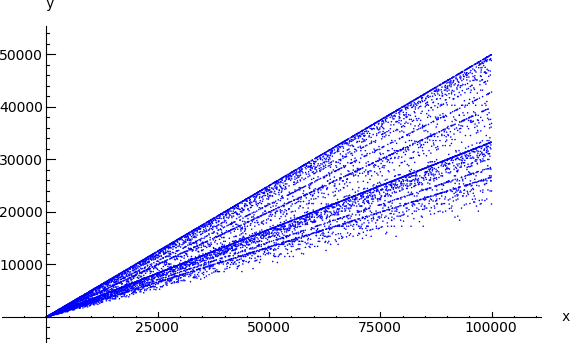
\includegraphics{figures/primitive-roots-all}
\caption{Die Anzahl der Primitivwurzeln f�r alle Primzahlen zwischen 1 und 100.000}
\label{fig:primitive_roots_all}
\end{figure}

\vskip +50 pt
Abbildung~\ref{fig:primitive_roots_smallest} gibt die kleinste Primitivwurzel
von jeder Primzahl zwischen 1 und 100.000 aus. Die $x$-Achse repr�sentiert
die Primzahlen 1 bis 100.000, die $y$-Achse gibt die kleinste Primitivwurzel
pro Primzahl aus.

\vskip +25 pt
Abbildung~\ref{fig:primitive_roots_largest} zeigt die entsprechende Graphik
mit der gr��ten Primitivwurzel zu jeder Primzahl im obigen Intervall.

\begin{figure}[!htbp]
\centering
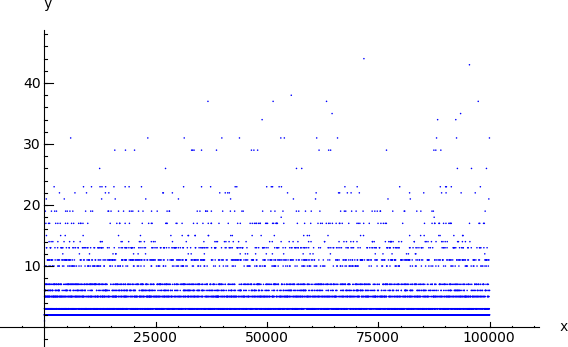
\includegraphics{figures/primitive-roots-smallest}
\caption{Die kleinste Primitivwurzel von jeder Primzahl zwischen 1 und 100.000}
\label{fig:primitive_roots_smallest}
\end{figure}

\begin{figure}[!htbp]
\centering
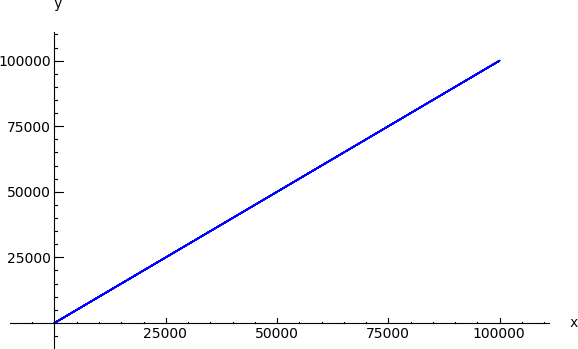
\includegraphics{figures/primitive-roots-largest}
\caption{Die gr��te Primitivwurzel von jeder Primzahl zwischen 1 und 100.000}
\label{fig:primitive_roots_largest}
\end{figure}

% To enforce that the next chapter starts at the beginning of a new page after
% the freely placed graphics, it was necessary to have TWO newpages and in between
% something to be printed (here invisible blanks).
% \newpage
% $ $
% I guess \clearpage is preferable.



% ---------------------------------------------------------------------------
\newpage
\hypertarget{NumberTheory_Sage_RSA sample}{}
\subsection{RSA-Beispiele mit Sage}
\label{l:NumberTheory_Sage_RSA sample}{}

\noindent In diesem Abschnitt sind die Sage-Quelltexte f�r die einfachen RSA-Beispiele
im Kapitel~\ref{rsaconcrete} (``\nameref{rsaconcrete}'') angegeben. 

\vskip +10 pt 
\hypertarget{AppArith4a}{%
\noindent \textbf{Beispiel auf Seite~\pageref{SrcArith4a}:}} \\
Die RSA-Exponentiation $M^{37} \pmod{3713}$ f�r die Nachricht $M = 120$ kann
mit Sage folgenderma�en ausgef�hrt werden:

\begin{Verbatim}%
[fontsize=\footnotesize,fontshape=tt]
sage: power_mod(120, 37, 3713)
1404
\end{Verbatim}


\vskip +10 pt 
\hypertarget{AppArith4b}{%
\noindent {\bf Beispiel auf Seite~\pageref{SrcArith4b}:}} \\

Die Faktorisierung von $J(256.027) = 255.016 = 2^3 * 127 * 251$ kann mit Sage
folgenderma�en durchgef�hrt werden:

\begin{sagecode}
\begin{Verbatim}%
[fontsize=\footnotesize,fontshape=tt]
sage: factor(255016)
2^3 * 127 * 251
\end{Verbatim}
\caption{Faktorisierung einer Zahl}
\end{sagecode}


\vskip +10 pt 
\hypertarget{AppArith4c}{%
\noindent {\bf Beispiel auf Seite~\pageref{SrcArith4c}:}} \\
RSA-Verschl�sselung mit Sage:

\begin{sagecode}
\begin{Verbatim}%
[fontsize=\footnotesize,fontshape=tt]
sage: A = [82, 83, 65, 32, 119, 111, 114, 107, 115, 33]
sage: e = 65537; m = 256027
sage: [power_mod(a, e, m) for a in A]
[212984, 25546, 104529, 31692, 248407, 100412, 54196, 100184, 58179, 227433]
\end{Verbatim}
\caption{RSA-Verschl�sselung durch modulare Exponentiation einer Zahl (als Nachricht)}
\end{sagecode}


\vskip +10 pt 
\hypertarget{AppArith4d}{%
\noindent {\bf Beispiel auf Seite~\pageref{SrcArith4d}:}} \\
RSA-Verschl�sselung mit Sage:

\begin{Verbatim}%
[fontsize=\footnotesize,fontshape=tt]
sage: A = [21075, 16672, 30575, 29291, 29473]
sage: e = 65537; m = 256027
sage: [power_mod(a, e, m) for a in A]
[158721, 137346, 37358, 240130, 112898]
\end{Verbatim}


\vskip +10 pt 
\hypertarget{AppArith4e}{%
\noindent {\bf Beispiel auf Seite~\pageref{SrcArith4e}:}} \\
RSA-Verschl�sselung mit Sage:

\begin{Verbatim}%
[fontsize=\footnotesize,fontshape=tt]
sage: A = [82083, 65032, 119111, 114107, 115033]
sage: e = 65537; m = 256027
sage: [power_mod(a, e, m) for a in A]
[198967, 51405, 254571, 115318, 14251]
\end{Verbatim}




% ---------------------------------------------------------------------------
\newpage
\hypertarget{NumberTheory_Sage_Number-of-RSA-keys}{}
\subsection{Wie viele RSA-Schl�ssel gibt es innerhalb eines Modulo-Bereiches?}
\label{l:NumberTheory_Sage_Number-of-RSA-keys}{}

Die RSA-Verschl�sselung wurde beschrieben in Abschnitt \ref{RSA} (``\nameref{RSA}'').
Schritt 1 bis 3 definieren die Schl�sselerzeugung, Schritt 4 und 5 stellen die
eigentliche Verschl�sselung dar:
\begin{itemize}
  \item[{\bf 1.}] W�hle zwei unterschiedliche Primzahlen $p$ and $q$
                  und berechne $n = p*q$.\\
                  Der Wert $n$ wird RSA-Modul genannt.

  \item[{\bf 2.}] W�hle ein zuf�lliges $e \in \{2, \cdots, n-1\}$, so dass gilt: \\
                  $e$ ist relativ prim zu $J(n) = (p-1)*(q-1)$. \\
                  Danach kann man $p$ und $q$ \glqq wegwerfen\grqq.

  \item[{\bf 3.}] W�hle $d \in \{1, \cdots, n-1\}$ mit $e*d \equiv 1  
                  {\rm ~(mod~} J(n))$,\\
		  d.h. $d$ ist die multiplikative Inverse von $e$ modulo $J(n)$.
		  Dann kann man $J(n)$ \glqq wegwerfen\grqq.
    \begin{itemize}
      \item[] $\rightarrow (n, e)$ ist der �ffentliche Schl�ssel $P$.
      \item[] $\rightarrow (n, d)$ ist der private Schl�ssel $S$ (nur $d$ muss man geheim halten).
    \end{itemize}

  \item[{\bf 4.}] Zur Verschl�sselung wird die Nachricht als (bin�re) Ziffernfolge
                  geschrieben. Diese Ziffernfolge wird dann so in gleich lange Teilfolgen
		  aufgeteilt, dass jede Teilfolge eine Zahl kleiner als $n$ darstellt.

  \item[{\bf 5.}] Vorgang der Verschl�sselung auf dem Klartext (bzw. auf Teilen davon)
                  $M \in \{1, \cdots, n-1\}$:
                  $$C = E ( (n, e); M ) := M^e {\rm ~(mod~} n).$$
\end{itemize}

Standardm��ig versucht man, einen mit RSA verschl�sselten Geheimtext $C$ dadurch zu knacken,
dass man den �ffentlichen Schl�ssel des Empf�ngers betrachtet und versucht, $n$ zu
faktorisieren. Hat man das erreicht, geht man wieder durch die Schritte 2 und 3 und
erzeugt den privaten Schl�ssel $e$, den man zum Entschl�sseln des Geheimtextes braucht.

Gem�� dem \glqq Primzahlsatz\grqq (beschrieben in Abschnitt \ref{thm-pz-pi-x}
\glqq \nameref{thm-pz-pi-x}\grqq) bewegt sich die Anzahl der Primzahlen
$PI(x)$ asymptotisch gegen  $x / ln(x)$.
F�r ein gegebenes $n$ gibt es also ca. $n / ln(n)$ m�gliche Werte f�r die
Primzahl $p$.

\noindent Will man nicht faktorisieren, sondern stellt sich eine Frage �hnlich
wie bei den klassischen Verschl�sselungsverfahren, kann man herausfinden wollen:
Wie viele verschiedene private Schl�ssel $(n, d)$ gibt es f�r einen bestimmten
Bereich der Schl�sselgr��e $n \in [a, b]$?

\noindent Das Sage-Beispielprogramm~\ref{nt_sagesample_Count_RSA_Keys} unten definiert
die Funktion \verb#count_Number_of_RSA_Keys#, die diese Frage konkret beantworten kann
(wenn der Modulus nicht zu gro� ist).\footnote{%
a) Der Aufruf \verb#sage: count_Number_of_RSA_Keys(100, 1000)# bedeutet, dass man
das Intervall $[100, 1000]$ f�r $n$ betrachtet.
$n$ war definiert durch die beiden Primzahlen $p, q: n = p*q$.
Daher kann eine Primzahl h�chstens den Wert $500$ annehmen, weil $2 * 500 =1000$.\\
Die Anzahl m�glicher Primzahl-Kombinationen betr�gt: $comb = 258$.\\
Die Anzahl der Primzahlen im gegebenen Bereich betr�gt: $143$.\\
Die Anzahl der privaten Schl�ssel betr�gt: $34.816$.

\noindent b) Der Aufruf \verb#sage: count_Number_of_RSA_Keys(100, 100, True)#
hat die folgende Ausgabe:\\
   - Number of private keys for modulus in a given range: 0\\
   - Number of primes in a given range: 0\\
   Der Grund daf�r ist, dass wir damit nur $n=100$ betrachten, und $100$ ist nicht
   semi-prim\index{Primzahl!semi-prim}\index{Primzahl!Halbprimzahl},
   d.h. $100$ ist nicht das Produkt von genau zwei Primzahlen.
}


\begin{sagecode}
\begin{Verbatim}%
[fontsize=\footnotesize,fontshape=tt]
def count_Number_of_RSA_Keys(start, end, Verbose=False):
      r"""
      How many private RSA keys (n,d) exist, if only modulus N is given, and start <= N <= end?
        (prime_range(u,o) delivers all primes >=u und < o).
      """
      a = start
      b = end
      s = 0
      comb = 0
      for p in prime_range(1, b/2+1):
          for q in prime_range(p + 1, b/2+1):
              if a <= p * q and p * q <= b:
                  comb = comb +1
                  s = s + (euler_phi(euler_phi(p * q))-1)
                  if Verbose:
                      print "p=%s, " % p + "q=%s, " % q + "s=%s" % s
      print "Number of private keys for modulus in a given range: %s" % s + " (comb=%s), " % comb

      # Just for comparison: How many primes are in this range?
      s = 0
      for p in prime_range(a, b+1):
          if Verbose:
              print "a=%s, " % a + "b=%s, " % b + "p=%s" % p
          s = s + 1
      print "Number of primes in a given range: %s" % s

print "\n\nDD_Start -- Testcases for count_Number_of_RSA_Keys(start, end)"
print "\n-----------Testcase: (100, 1000) [Should deliver 34.816]"
time count_Number_of_RSA_Keys(100, 1000)
print "\n-----------Testcase: (100, 107, True) [Should deliver 23]"
time count_Number_of_RSA_Keys(100, 107, True)
u = 10^3; o = 10^4;
print "\n-----------Testcase: (%s, " % u + "%s) [Should deliver 3.260.044]" % o
time count_Number_of_RSA_Keys(u, o)

OUTPUT:
DD_Start -- Testcases for count_Number_of_RSA_Keys(start, end)

-----------Testcase: (100, 1000) [Should deliver 34.816]
Number of private keys for modulus in a given range: 34816 (comb=258),
Number of primes in a given range: 143
Time: CPU 0.03 s, Wall: 0.04 s

-----------Testcase: (100, 107, True) [Should deliver 23]
p=2, q=53, s=23
Number of private keys for modulus in a given range: 23 (comb=1),
a=100, b=107, p=101
a=100, b=107, p=103
a=100, b=107, p=107
Number of primes in a given range: 3
Time: CPU 0.00 s, Wall: 0.00 s

-----------Testcase: (1000, 10000) [Should deliver 3.260.044]
Number of private keys for modulus in a given range: 3260044 (comb=2312),
Number of primes in a given range: 1061
Time: CPU 0.63 s, Wall: 0.66 s
\end{Verbatim}
\caption{Wie viele RSA-Schl�ssel gibt es, wenn man den Bereich f�r die Schl�sselgr��e n kennt?}
\label{nt_sagesample_Count_RSA_Keys}
\end{sagecode}

\noindent Weil es mehr private Schl�ssel $(n, d)$ innerhalb eines gr��eren
Bereiches von Werten f�r $n$ gibt, ist das Brute-force-Faktorisieren
viel effizienter als das Durchprobieren aller m�glichen Schl�ssel.




% ++++++++++++++++++++++++++++++++++++++++++++++++++++++++++++++++++++++++++
\clearpage
\newpage
\hypertarget{NumberTheory_Appendix_F}{}  %\hypertarget{AppendixListAndDef}{}
\section{Anhang: Liste der in diesem Kapitel formulierten Definitionen und S�tze}
\label{l:NumberTheory_Appendix_F}{}  %\label{l:AppendixListAndDef}{}

% \vskip +8 pt
\begin{center}
\begin{tabular}{|l|l|l|}\hline
 & Kurzbeschreibung~~ & Seite \\ \hline
Definition~\ref{def-zth-prime} & Primzahlen &  \pageref{def-zth-prime} \\
Definition~\ref{def-zth-composite} & Zusammengesetzte Zahlen
                                   & \pageref{def-zth-composite}  \\ \hline
Satz~\ref{thm-zth-cnum} & Teiler von zusammengesetzten Zahlen~~~~~~~ & \pageref{thm-zth-cnum}\\
Satz~\ref{thm-zth-mthm} &  Erster Hauptsatz der elementaren Zahlentheorie &  \pageref{thm-zth-mthm} \\  \hline
Definition~\ref{def-zth-divisibility} & Teilbarkeit & \pageref{def-zth-divisibility} \\
Definition~\ref{def-zth-remainder} & Restklasse $r$ modulo $m$ & \pageref{def-zth-remainder} \\
Definition~\ref{def-zth-congruence} & restgleich oder kongruent & \pageref{def-zth-congruence} \\ \hline
Satz~\ref{thm-zth-div} & Kongruenz mittels Differenz & \pageref{thm-zth-div} \\
Satz~\ref{thm-zth-multinv} & Multiplikative Inverse (Existenz) & \pageref{thm-zth-multinv}  \\
Satz~\ref{thm-zth-exhperm} & Ersch�pfende Permutation & \pageref{thm-zth-exhperm} \\
Satz~\ref{thm-zth-pot} & Gestaffelte Exponentiation mod $m$ & \pageref{thm-zth-pot} \\ \hline
Definition~\ref{def-zth-zn} & $\mathbb{Z}_n$  & \pageref{def-zth-zn}\\
Definition~\ref{def-zth-znmult} &   $\mathbb{Z}_n^*$ & \pageref{def-zth-znmult} \\ \hline
Satz~\ref{thm-zth-znmult} & Multiplikative Inverse in $\mathbb{Z}_n^*$& \pageref{thm-zth-znmult} \\ \hline
Definition~\ref{def-zth-phiofn} & Euler-Funktion $J(n)$ & \pageref{def-zth-phiofn} \\
Satz~\ref{thm-zth-phiprime} & $J(p)$ &  \pageref{thm-zth-phiprime}\\
Satz~\ref{thm-zth-phipq} & $J(p*q)$ &  \pageref{thm-zth-phipq}\\
Satz~\ref{thm-zth-phimultprime} & $J(p_1 * \cdots *p_k)$ & \pageref{thm-zth-phimultprime} \\
Satz~\ref{thm-zth-phinum} & $J(p_1^{e_1} * \cdots *p_k^{e_k})$ & \pageref{thm-zth-phinum} \\
Satz~\ref{thm-zth-fermat1} & Kleiner Satz von Fermat &  \pageref{thm-zth-fermat1}\\
Satz~\ref{thm-zth-fermateuler} & Satz von Euler-Fermat & \pageref{thm-zth-fermateuler} \\ \hline
Definition~\ref{def-zth-ordn} & Multiplikative Ordnung $ {\rm ord}_{m} (a)$ & \pageref{def-zth-ordn} \\
Definition~\ref{def-zth-primitiveroot} & Primitivwurzel von $m$ &  \pageref{def-zth-primitiveroot}\\
Satz~\ref{thm-zth-ordp} & Aussch�pfung des Wertebereiches & \pageref{thm-zth-ordp} \\ \hline
\end{tabular}
\end{center}
\vskip +6 pt





% ++++++++++++++++++++++++++++++++++++++++++++++++++++++++++++++++++++++++++
% ++++++++++++++++++++++++++++++++++++++++++++++++++++++++++++++++++++++++++
\newpage
%\addcontentsline{toc}{section}{Literaturverzeichnis}
\begin{thebibliography}{99999}
\addcontentsline{toc}{section}{Literaturverzeichnis}

\bibitem[Agrawal2002]{nt:Agrawal2002}  \index{Agrawal 2002} 
    M. Agrawal, N. Kayal, N. Saxena, \\
    {\em PRIMES in P}, August 2002, Korrigierte Fassung: \\
       \href{http://www.cse.iitk.ac.in/~manindra/algebra/primality_v6.pdf}
    {\texttt{http://www.cse.iitk.ac.in/~manindra/algebra/primality\_v6.pdf}} \\
    Siehe auch die Seite \glqq The AKS \glqq PRIMES in P'' Algorithm Resource'':
       \href{http://fatphil.org/maths/AKS/}
    {\texttt{http://fatphil.org/maths/AKS/}}

\bibitem[Bartholome1996]{nt:Bartholome1996} \index{Bartholome 1996}  
    A. Bartholom\'e, J. Rung, H. Kern, \\
    {\em Zahlentheorie f�r Einsteiger}, Vieweg 1995, 2. Auflage 1996.

\bibitem[Bauer1995]{nt:Bauer1995} \index{Bauer 1995}
    Friedrich L. Bauer, \\
    {\em Entzifferte Geheimnisse}, Springer, 1995.

\bibitem[Bauer2000]{nt:Bauer2000} \index{Bauer 2000}
    Friedrich L. Bauer, \\
    {\em Decrypted Secrets}, Springer 1997, 2nd edition 2000.

\bibitem[Bernstein2001]{nt:Bernstein2001} \index{Bernstein 2001}
    D.~J. Bernstein, \\
    {\em Circuits for integer factorization: a proposal},\\ 
    \href{http://cr.yp.to/papers/nfscircuit.ps}
    {\texttt{http://cr.yp.to/papers/nfscircuit.ps}} \\
    \href{http://cr.yp.to/djb.html}{\texttt{http://cr.yp.to/djb.html}}

\bibitem[Beutelspacher1996]{nt:Beutelspacher1996} \index{Beutelspacher 1996}
    Albrecht Beutelspacher, \\
    {\em Kryptologie}, Vieweg 1987, 5. Auflage 1996.

\bibitem[Bourseau2002]{nt:Bourseau2002} \index{Bourseau 2002} \index{Fox 2002}
    F. Bourseau, D. Fox, C. Thiel, \\
    {\em Vorz�ge und Grenzen des RSA-Verfahrens},\\
    In: Datenschutz und Datensicherheit (DuD) 26/2002, S. 84-89 (s. www.dud.de),
    \href{http://http://www.secorvo.de/publikationen/rsa-grenzen-fox-2002.pdf}
         {\texttt{http://www.secorvo.de/publikationen/rsa-grenzen-fox-2002.pdf}}

\bibitem[Brands2002]{nt:Brands2002} \index{Brands 2002}
    Gilbert Brands, \\
    {\em Verschl�sselungsalgorithmen -- Angewandte Zahlentheorie 
    rund um Sicherheitsprotokolle}, Vieweg, 2002.

\bibitem[BSI2002]{nt:BSI2002} \index{BSI 2002}
    BSI (Bundesamt f�r Sicherheit in der Informationstechnik), \\
    {\em Empfehlungen zur Wahl der Schl�ssell�ngen}, Bonn, 9.9.2002, \\
    (Geeignete Kryptoalgorithmen zur Erf�llung der Anforderungen
    nach \S 17 (1) SigG vom 22. Mai 2001 in Verbindung mit Anlage 1, 
    I 2, SigV vom 22. November 2001), \\
    \href{http://www.bsi.bund.de/esig/basics/techbas/krypto/bund02v7.pdf}
    {\tt http://www.bsi.bund.de/esig/basics/techbas/krypto/bund02v7.pdf} \\
    Eine Stellungnahme zu diesen Empfehlungen: \\
    \href{http://www.secorvo.de/publikat/stellungnahme-algorithmenempfehlung-020307.pdf}
    {\texttt{http://www.secorvo.de/publikat/}}\\
    \hspace*{1cm}
    \href{http://www.secorvo.de/publikat/stellungnahme-algorithmenempfehlung-020307.pdf}
    {\texttt{stellungnahme-algorithmenempfehlung-020307.pdf}}

\bibitem[Buchmann2004]{nt:Buchmann2004} \index{Buchmann 2004}
    Johannes Buchmann, \\
    {\em Einf�hrung in die Kryptographie}, Springer, 3. Auflage, 2004.

\bibitem[Buhler1993]{nt:Buhler1993} \index{Buhler 1993} 
    J.P. Buhler, H.W. Lenstra, C. Pomerance, \\
    {\em Factoring integers with the number field sieve}, \\
    In: A.K. Lenstra, H.W. Lenstra (Hrsg.): The Development of the 
    Number Field Sieve, Lecture Notes in Mathematics, Vol.~1554, 
    Springer, Heidelberg 1993, S. 50$-$94.

\bibitem[Eckert2003]{nt:Eckert2003} \index{Eckert 2003} 
    Claudia Eckert, \\
    {\em IT-Sicherheit: Konzepte-Verfahren-Protokolle}, 
    Oldenbourg 2001, 2. Auflage 2003.

\bibitem[Ertel2001]{nt:Ertel2001} \index{Ertel 2001} 
    Wolfgang Ertel, \\
    {\em Angewandte Kryptographie}, 
    Fachbuchverlag Leipzig FV 2001.

\bibitem[Graham1994]{nt:Graham1994} \index{Graham 1994}
     Graham, Knuth, Patashnik, \\
     {\em Concrete Mathemathics, a Foundation of Computer Science}, \\
     Addison Wesley 1989, 6th printing 1994.

\bibitem[Kippenhahn1997]{nt:Kippenhahn1997} \index{Kippenhahn 1997}
    Rudolph Kippenhahn, \\
    {\em Verschl�sselte Botschaften -- Geheimschrift, Enigma und Chipkarte}, 
    Rowohlt, 1997.

\bibitem[Kippenhahn1999]{nt:Kippenhahn1999} \index{Kippenhahn 1999}
    Rudolph Kippenhahn, \\
    {\em Code Breaking -- A History and Exploration}, 
    Constable, 1999.

\bibitem[Knuth1998]{nt:Knuth1998} \index{Knuth 1998}
    Donald E. Knuth, \\
    {\em The Art of Computer Programming, vol 2: Seminumerical Algorithms}, \\
    Addison-Wesley, 2nd edition 1998.
    % Wann war die erste Edition ?

\bibitem[Lenstra1993]{nt:Lenstra1993} \index{Lenstra 1993}
     A. Lenstra, H. Lenstra: \\ 
     {\em The development of the Number Field Sieve}, \\
     Lecture Notes in Mathematics 1554, Springer, New York 1993

\bibitem[Lenstra1999]{nt:Lenstra1999} Arjen K. Lenstra, Eric R. Verheul,
     \index{Lenstra/Verheul 1999} \\
     {\em Selecting Cryptographic Key Sizes (1999)}, \\
     Journal of Cryptology: the journal of the International 
     Association for Cryptologic Research \\
     \href{http://www.cryptosavvy.com/cryptosizes.pdf}
     {\texttt{http://www.cryptosavvy.com/cryptosizes.pdf}}

\bibitem[Lenstra2002]{nt:Lenstra2002} \index{Lenstra 2002}
    Arjen K. Lenstra, Adi Shamir, Jim Tomlinson, Eran Tromer,\\
    {\em Analysis of Bernstein's Factorization Circuit},\\
    \href{http://www.cryptosavvy.com/mesh.pdf}
    {\texttt{http://www.cryptosavvy.com/mesh.pdf}}

\bibitem[Menezes2001]{nt:Menezes2001} \index{Menezes 2001}
    Alfred J. Menezes, Paul C. van Oorschot, Scott A. Vanstone \\
    {\em Handbook of Applied Cryptography}, 
    CRC Press 1997, 5th printing 2001.

\bibitem[Pfleeger1997]{nt:Pfleeger1997} \index{Pfleeger 1997}
    Charles P. Pfleeger, \\
    {\em Security in Computing}, Prentice-Hall, 2nd edition 1997.
    % Im Buch stand nicht, wann die 1. Edition rauskam.

\bibitem[Pomerance1984]{nt:Pomerance1984} \index{Pomerance 1984} 
    C. Pomerance, \\
    {\em The quadratic sieve factoring algorithm}, \\
    In: G.R. Blakley, D. Chaum (Hrsg.): Proceedings of Crypto '84, 
    LNCS 196, Springer Berlin 1995, S. 169-182.

\bibitem[RSA Security 2002]{nt:RSA Security 2002} \index{RSA Security 2002} 
    RSA Security, \\
    {\em Has the RSA algorithm been compromised as a result 
    of Bernstein's Paper?}, \\
    8. April 2002, \\
    \href{http://www.rsasecurity.com/}{\tt http://www.rsasecurity.com/}.

\bibitem[SchneiderM2004]{nt:SchneiderM2004} \index{SchneiderM 2004} 
    Matthias Schneider, \\
    {\em Analyse der Sicherheit des RSA-Algorithmus. \\
     M�gliche Angriffe, deren Einfluss auf sichere Implementierungen
     und �konomische Konsequenzen}, \\
    Diplomarbeit an der Universit�t Siegen, 2004.

\bibitem[Schneier1996]{nt:Schneier1996nt} \index{Schneier 1996} 
    Bruce Schneier, \\
    {\em Applied Cryptography, Protocols, Algorithms, and Source Code in C}, \\
    Wiley and Sons 1994, 2nd edition 1996.

\bibitem[Schwenk2002]{nt:Schwenk2002}\index{Schwenk 2002}
    J�rg Schwenk, \\
    {\em Sicherheit und Kryptographie im Internet}, 
    Vieweg 2002.

\bibitem[Sedgewick1990]{nt:Sedgewick1990} \index{Sedgewick 1990}
    Robert Sedgewick,\\
    {\em Algorithms in C}, Addison-Wesley, 1990.

\bibitem[Shamir2003]{nt:Shamir2003} \index{Shamir 2003} \index{TWIRL-Device} 
    Adi Shamir, Eran Tromer, \\
    {\em Factoring Large Numbers with the TWIRL Device}, 
    Januar 2003, \\
    \href{http://www.wisdom.weizmann.ac.il/~tromer/}
    {\texttt{http://www.wisdom.weizmann.ac.il/\~{}tromer/}}

\bibitem[Shamir2003a]{nt:Shamir2003a} \index{Shamir 2003a} \index{TWIRL-Device} 
    Adi Shamir, Eran Tromer, \\
    {\em On the Cost of Factoring RSA-1024}, 
    RSA Laboratories CryptoBytes Volume 6, No. 2, Summer 2003, S. 11-20 \\
    \href{http://www.rsasecurity.com/rsalabs/cryptobytes/CryptoBytes_August_2003.pdf}
    {\texttt{http://www.rsasecurity.com/rsalabs/cryptobytes/CryptoBytes\_August\_2003.pdf}}
  
\bibitem[Silverman2000]{nt:Silverman2000} \index{Silverman 2000}
     Robert D. Silverman: \\ 
     {\em A Cost-Based Security Analysis of Symmetric and Asymmetric 
          Key Lengths} \\ 
     In: RSA Laboratories Bulletin, No. 13, April 2000, S. 1-22

\bibitem[Stinson1995]{nt:3Stinson1995} \index{Stinson 1995}
    Douglas R. Stinson,\\
    {\em Cryptography - Theory and Practice}, CRC Press, 1995.

\bibitem[Weis2003]{nt:Weis2003} \index{Weis 2003} \index{Lucks 2003} \index{Bogk 2003}
    R�diger Weis, Stefan Lucks, Andreas Bogk, \\
    {\em Sicherheit von 1024 bit RSA-Schl�sseln gef�hrdet},\\
    In: Datenschutz und Datensicherheit (DuD) 6/2003, S. 360-362 (s. www.dud.de)\\
    Der Artikel erl�utert Details zum TWIRL-Device\index{TWIRL-Device}.

\bibitem[Welschenbach2001]{nt:Welschenbach2001} \index{Welschenbach 2001}
    Welschenbach, Michael, \\
    {\em Kryptographie in C und C++}, Springer 2001.

\bibitem[Wiles1994]{nt:Wiles1994} \index{Wiles, Andrew}
    Wiles, Andrew, \\
    {\em Modular elliptic curves and Fermat's Last Theorem}%
    \index{Fermat!letzter Satz}, \\
    In: Annals of Mathematics 141 (1995).

\bibitem[Wolfenstetter1998]{nt:Wolfenstetter1998} \index{Wolfenstetter 1998}
    Albrecht Beutelspacher, J�rg Schwenk, Klaus-Dieter Wolfenstetter, \\
    {\em Moderne Verfahren in der Kryptographie}, 
    Vieweg 1995, 2. Auflage 1998.

\bibitem[Yan2000]{nt:Yan2000} \index{Yan 2000} 
    Song Y. Yan, \\
    {\em Number Theory for Computing}, Springer, 2000.
    
\end{thebibliography}



% ++++++++++++++++++++++++++++++++++++++++++++++++++++++++++++++++++++++++++
\newpage
\section*{Web-Links}\addcontentsline{toc}{section}{Web-Links}

\begin{enumerate}
   \item \hypertarget{knott}{} \index{Knott, Ron}
          Fibonacci-Seite \index{Fibonacci} von Ron Knott, \\
          Hier dreht sich alles um Fibonacci-Zahlen. \\
          \href{http://www.mcs.surrey.ac.uk/personal/R.Knott/Fibonacci/fib.html}
	  {\texttt{http://www.mcs.surrey.ac.uk/personal/R.Knott/Fibonacci/fib.html}}
          
   \item CrypTool,  \index{CrypTool} \\
          E-Learning-Freeware zur Veranschaulichung von Kryptographie
          und Kryptoanalyse, \\
          \href{http://www.cryptool.de}{\texttt{http://www.cryptool.de}}, \\
          \href{http://www.cryptool.org}{\texttt{http://www.cryptool.org}},\\ 
          \href{http://www.cryptool.com}{\texttt{http://www.cryptool.com}}
          
   \item Mathematica, \index{Mathematica} \\
          Kommerzielles Mathematik-Paket \\
          \href{http://www.wolfram.com}{\texttt{http://www.wolfram.com }}
          
   \item  LiDIA, \index{LiDIA} \\ 
          Umfangreiche Bibliothek mit zahlentheoretischen Funktionen und dem
          Interpreter LC \\
          \href{http://www.informatik.tu-darmstadt.de/TI/LiDIA}
          {\texttt{http://www.informatik.tu-darmstadt.de/TI/LiDIA}}
          
   \item BC, \index{BC} \\
         Interpreter mit zahlentheoretischen Funktionen \\
         \href{http://www.gnu.org/software/bc/bc.html}
         {\texttt{http://www.gnu.org/software/bc/bc.html}}
         %Check 11.5.07: nicht mehr zug�nglich.
         %\href{http://www.maths.uq.edu.au/~krm/gnubc.html}
         %{\texttt{http://www.maths.uq.edu.au/\~{}}krm/gnubc.html}
         
   \item Pari-GP, \index{Pari-GP} \\
         Hervorragender, schneller und freier Interpreter mit
         zahlentheoretischen Funktionen. \\ 
         \href{http://pari.math.u-bordeaux.fr/}
              {\texttt{http://pari.math.u-bordeaux.fr/}}\\
         \href{http://en.wikipedia.org/wiki/PARI/GP}
              {\texttt{http://en.wikipedia.org/wiki/PARI/GP}}\\
         Ressourcen zu PARI/GP auf der Webseite von Karim Belabas:\\
         \href{http://www.math.u-bordeaux.fr/~belabas/pari/}
              {\texttt{http://www.math.u-bordeaux.fr/\~{}belabas/pari/}}

   \item \index{Munchenbach@M�nchenbach, Carsten}
         Erst nach Vollendung dieses Artikels wurde mir die Web-Seite von
         Herrn M�nchenbach bekannt, die interaktiv und didaktisch sehr
         ausgereift die grundlegenden Denkweisen der Mathematik anhand
         der elementaren Zahlentheorie nahebringt. Sie entstand f�r
         ein Unterrichtsprojekt der 11. Klasse des Technischen Gymnasiums
         (leider nur in Deutsch verf�gbar): \\
         \href{http://www.hydrargyrum.de/kryptographie}
         {\texttt{http://www.hydrargyrum.de/kryptographie}}
         
   \item Seite des Beauftragten f�r die Lehrplanentwicklung des Fachs
         Informatik an der gymnasialen Oberstufe des Landes Saarland.
         Hier befindet sich eine Sammlung von Texten und Programmen 
         (in Java), die aus didaktischen �berlegungen entstand (alles 
         leider nur in Deutsch verf�gbar). \\
         \href{http://www.saar.de/~awa/kryptolo.htm}
         {\texttt{http://www.saar.de/\~{}awa/kryptolo.htm}}
         
   \item BSI, \index{BSI}\\ 
         Bundesamt f�r Sicherheit in der Informationstechnik \\
         \href{http://www.bsi.bund.de}{\texttt{http://www.bsi.bund.de}}

   \item Faktorisierungsrekorde und Challenges\index{Faktorisierung!Faktorisierungsrekorde},\\
         \href{http://www.crypto-world.com/}
           {\texttt{http://www.crypto-world.com/}} \\
         \href{http://www.crypto-world.com/FactorWorld.html}
           {\texttt{http://www.crypto-world.com/FactorWorld.html}}, Webseite von Scott Contini \\
         \href{http://www.loria.fr/~zimmerma/records/factor.html}
           {\texttt{http://www.loria.fr/\~{}zimmerma/records/factor.html}} \\
         \href{http://www.tutorgig.com/ed/RSA\_number}
           {\texttt{http://www.tutorgig.com/ed/RSA\_number}} \\

         \href{http://www.uni-bonn.de/Aktuelles/Pressemitteilungen/pm02/pm035-02.html}
           {\texttt{http://www.uni-bonn.de/Aktuelles/Pressemitteilungen/pm02/pm035-02.html}} \\
         \href{http://www.ercim.org/publication/Ercim\_News/enw49/franke.html, 2002-01}
           {\texttt{http://www.ercim.org/publication/Ercim\_News/enw49/franke.html, 2002-01}} \\
         \href{http://www.loria.fr/~zimmerma/records/rsa160}
           {\texttt{http://www.loria.fr/\~{}zimmerma/records/rsa160}} \\

         \href{http://www.rsa.com/rsalabs/node.asp?id=2092}
           {\texttt{http://www.rsa.com/rsalabs/node.asp?id=2092}}
	 
   \item Das Cunningham-Projekt, \index{Cunningham-Projekt}\\ 
         \href{http://www.cerias.purdue.edu/homes/ssw/cun/}
         {\texttt{http://www.cerias.purdue.edu/homes/ssw/cun/}}

   \item Sage, \index{Sage} \\
         Ausgezeichnetes Open-Source Computer-Algebra-System, basierend auf Python
	 als Skript-Sprache. Damit sind die Code-Beispiele in diesem Kapitel erstellt.
	 Vergleiche die Einf�hrung in Kapitel~\ref{s:appendix-using-sage}.\\
         \href{http://www.sagemath.org/}
              {\texttt{http://www.sagemath.org/}}\\
         \href{http://en.wikipedia.org/wiki/Sage_%28mathematics_software%29}
              {\texttt{http://en.wikipedia.org/wiki/Sage\_\%28mathematics\_software\%29}}\\

\end{enumerate}



% ++++++++++++++++++++++++++++++++++++++++++++++++++++++++++++++++++++++++++
\vskip +20 pt
\section*{Dank} \addcontentsline{toc}{section}{Dank}
Ich m�chte hier die Gelegenheit nutzen, den folgenden Personen ganz 
herzlich zu danken: 
\begin{itemize}

  \item {Hr. Henrik Koy f�r das anregende und sehr konstruktive 
         Korrekturlesen und f�r die vielen Verbesserungen der ersten
	 Version dieses Artikels, und f�r die Hilfen bei TeX, ohne die
	 dieser Artikel nie in dieser Form erschienen w�re. \\
	 Au�erdem hat Hr. Koy in seiner Freizeit im CrypTool-Programm 
	 die komplexe Dialogbox zum RSA-Kryptosystem
%	 RSA-Krypto"-system   (TRENNUNG erzwingen)
	 designed und die dahinterliegende Logik entwickelt, mit der die
	 RSA-Beispiele dieses Artikels nachvollzogen werden k�nnen.}

  \item {J�rg Cornelius Schneider f�r die engagierte Unterst�tzung bei TeX und
         die mannigfaltigen Hilfen bei allen Arten von Programmier- und
	 Design-Problemen.}

  \item {Dr. Georg Illies f�r den Hinweis auf Pari-GP\index{Pari-GP}.}
  
  \item {Lars Fischer f�r seine Hilfe bei schnellem Pari-GP\index{Pari-GP}-Code
         f�r Primitivwurzeln.}
  
  \item {Minh Van Nguyen aus Australien f�r seine immer schnelle, kompetente und
         ausf�hrliche Hilfe bei den Sage\index{Sage}-Code-Beispielen in diesem
	 Kapitel.}

\end{itemize}



% Local Variables:
% TeX-master: "../script-de.tex"
% End:

\renewcommand{\CTBChapName}{(Chap ModernCrypto)}  % $Id$
\setcounter{satz}{0}
\setcounter{definition}{0}

\newcommand{\NT}{\vspace*{0.2\baselineskip}\\}
\newcommand{\HZ}{\vspace*{0.5\baselineskip}}
\newcommand{\R}{\text{I}\!\text{R}}
\newcommand{\N}{\text{I}\!\text{N}}
\newcommand{\Q}{\text{Q}\!\!\!\text{l}\,\,}
\newcommand{\C}{\text{C}\!\!\!\text{l}\,\,}
\newcommand{\K}{\text{I}\!\text{K}}
\newcommand{\Z}{\mathbf{\mathbb{Z}}}
%--------------------------------------- matheScript-Zeichen definieren
\newcommand{\fs}{\mathscr{F}}  
\newcommand{\es}{\mathscr{E}}  
\newcommand{\cs}{\mathscr{C}}  
\newcommand{\gs}{\mathscr{G}}
\newcommand{\is}{\mathscr{I}}
\newcommand{\os}{\mathscr{O}}
\newcommand{\ks}{\mathscr{K}}
\newcommand{\qs}{\mathscr{Q}}
\newcommand{\us}{\mathscr{U}}
\newcommand{\hs}{\mathscr{H}}
\newcommand{\ps}{\mathscr{P}}
\newcommand{\as}{\mathscr{A}}
\newcommand{\rs}{\mathscr{R}}
\newcommand{\bs}{\mathscr{B}}
%-------------------------------------
\newcommand{\PG}{\text{I}\!\text{P}}
\newcommand{\carre}{\square}
\newcommand{\ncarre}{/\negthickspace\negthickspace\square}
\newcommand{\ncarreq}{{\ncarre}_q}
\newcommand{\ncarree}{/\negthickspace\negthickspace\negthickspace\square}
\newcommand{\ncarrepi}{{\ncarre}_{p^i}}
\newcommand{\mc}[1]{{\cal #1}}
\newcommand{\Char}{\text{char}}
\newcommand{\Aut}{\text{Aut}}
\newcommand{\Fix}{\text{Fix}}
\newcommand{\Syl}{\text{Syl}}
\newcommand{\Bild}{\text{Bild}}
\newcommand{\ggt}{\text{ggT}}
\newcommand{\kgv}{\text{kgV}}
\newcommand{\Id}{\text{Id}}
\newcommand{\nqcarre}{{\ncarre}_{q^2}}

\setlength{\fboxrule}{.4pt}
\setlength{\fboxsep}{4pt}

\newpage
%**************************************************************************************************************************
\section{Die mathematischen Ideen hinter der modernen Kryptographie}
%**************************************************************************************************************************
(Oyono R./ Esslinger B., Sep. 2000, Updates Nov. 2000, Feb. 2003)
%--------------------------------------------------------------------------------------------------------------------------
       \subsection{Einwegfunktionen mit Fallt"ur und Komplexit"atsklassen}
%--------------------------------------------------------------------------------------------------------------------------
\index{Kryptographie!moderne} \index{Einwegfunktion}
Eine {\bf Einwegfunktion} \hypertarget{Einwegfunktionen1}{} ist eine effizient zu 
berechnende (injektive) Funktion, deren Umkehrung jedoch nur mit 
extrem hohem Rechenaufwand -- jedoch praktisch unm"oglich -- zu berechnen ist.\par

Etwas genauer formuliert:  Eine Einwegfunktion ist eine Abbildung $ f $ einer Menge $ X $ in eine Menge $ Y, $ so dass $ f(x) $ f"ur jedes Element $ x $ von $ X $ leicht zu berechnen ist, w"ahrend es f"ur (fast) jedes $ y $ aus $ Y $  praktisch unm"oglich ist, ein Urbild $ x $ (d.h. ein $ x $ mit $ f(x)=y $) zu finden.\par

Ein allt"agliches Beispiel f"ur eine Einwegfunktion ist ein Telefonbuch: die auszuf"uhrende Funktion ist die, einem Namen die entsprechende Telefonnummer zuzuordnen. Da die Namen alphabetisch geordnet sind, ist diese Zuordnung einfach auszuf"uhren. Aber ihre Invertierung, also die Zuordnung eines Namens zu einer gegebenen Nummer, ist offensichtlich schwierig, wenn man nur ein Telefonbuch zur Verf"ugung hat. \par

Einwegfunktionen spielen in der Kryptographie eine entscheidende Rolle. Fast alle kryptographischen Begriffe kann man durch Verwendung des Begriffs Einwegfunktion umformulieren. Als Beispiel betrachten wir die Public Key-Verschl"usselung \index{Verschl""usselung!Public Key} (asymmetrische Kryptographie):\par

Jedem Teilnehmer $ T $ des Systems wird ein privater \index{Schl""ussel!privat}
\index{Schl""ussel!""offentlich} Schl"ussel $d_T$~\mbox{und} ein sogenannter "offentlicher Schl"ussel $ e_T $   zugeordnet. Dabei muss die folgende Eigenschaft (Public Key-Eigenschaft) gelten:\\
F"ur einen Gegner, der den "offentlichen Schl"ussel $ e_T $  kennt, ist es praktisch unm"oglich, den privaten Schl"ussel  $ d_T $ zu bestimmen.\par

Zur Konstruktion n"utzlicher Public Key-Verfahren sucht man also eine Einwegfunktion, die in einer Richtung \glqq einfach\grqq {} zu berechnen, die in der anderen Richtung jedoch \glqq schwer\grqq {} (praktisch unm"oglich) zu berechnen ist, solange eine bestimmte zus"atzliche Information \index{Einwegfunktion!mit Fallt""ur} (Fallt"ur) nicht zur Verf"ugung steht. Mit der zus"atzlichen Information kann die Umkehrung effizient gel"ost werden. Solche Funktionen nennt man {\bf Einwegfunktionen mit Fallt"ur} (trapdoor one-way function). Im obigen Fall ist $ d_T $ die Fallt"ur-In"-for"-ma"-tion. \par

Dabei bezeichnet man ein Problem als \glqq einfach\grqq, wenn es in \index{Laufzeit!polynomial} polynomialer Zeit als Funktion der L"ange der Eingabe l"osbar ist, d.h. wenn es so gel"ost werden kann, dass der Zeitaufwand sich als polynomiale Funktion in Abh"angigkeit der L"ange der Eingabe darstellen l"�sst. 
Wenn die L"ange der Eingabe $ n $ Bits betr"agt, so ist die Zeit der Berechnung der Funktion proportional zu $ n^{a}, $ wobei $ a $  eine Konstante ist. Man sagt, dass die \index{Komplexit""at} Komplexit"at solcher Probleme $ O(n^{a}) $ betr"agt (Landau- oder Big-O-Notation). 

Vergleicht man 2 Funktionen  $ 2^n $  und   $ n^{a} $, wobei $ a $  
eine Konstante ist, dann gibt es immer einen Wert f"ur  $ n $, ab dem
f"ur alle weiteren $ n $ gilt: $ n^{a}  <  2^n $. 
Die Funktion  $ n^{a} $  hat eine geringere Komplexit"at.
Z.B. f"ur $ a=5 $ gilt: ab der L"ange $ n=23 $ ist 
$ 2^n > n^5 $ ~\mbox{und} danach w"achst $ 2^n $ auch deutlich 
schneller \
[($ 2^{22}= 4.194.304 $, $ 22^5= 5.153.632 $); \
 ($ 2^{23}= 8.388.608 $, $ 23^5= 6.436.343 $); \
 ($ 2^{24}=16.777.216 $, $ 24^5= 7.962.624 $);].\par 
% "\mbox" nur, weil bei Ausdruck bei be die Blanks stets falsch sa�en:
%  "n^5un d"

Der Begriff \glqq praktisch unm"oglich\grqq {} ist etwas schwammiger. 
Allgemein kann man sagen, ein Problem ist \index{Laufzeit!effizient}
nicht effizient l"osbar, wenn der zu seiner L"osung ben"otigte Aufwand
schneller w"achst als die polynomiale Zeit als Funktion der Gr"o"se der
Eingabe. Wenn beispielsweise die L"ange der Eingabe $ n $  Bits betr"agt
und die Zeit zur Berechnung der Funktion proportional zu $ 2^n $ ist, 
so gilt gegenw"artig: die Funktion ist f"ur $n > 80$ praktisch nicht zu 
berechnen.

Die Entwicklung eines praktisch einsetzbaren Public Key-Verfahrens h"angt daher von der Entdeckung einer geeigneten Einwegfunktion mit Fallt"ur ab.\par

Um Ordnung in die verwirrende Vielfalt von m"oglichen Problemen und ihre Komplexit"aten zu bringen, fasst man Probleme mit "ahnlicher Komplexit"at zu Klassen zusammen.

Die wichtigsten Komplexit"atsklassen  sind die Klassen \textbf{P} und \textbf{NP}: 

\begin{itemize}

    \item Die Klasse \textbf{P}: Zu dieser Klasse geh"oren diejenigen Probleme, die mit polynomialem Zeitaufwand l"osbar sind.
    
    \item Die Klasse \textbf{NP}: Bei der Definition dieser Klasse betrachten wir nicht den Aufwand zur L"osung eines Problems, sondern den Aufwand zur Verifizierung einer gegebenen L"osung. Die Klasse \textbf{NP} besteht aus denjenigen Problemen, bei denen die Verifizierung einer gegebenen L"osung mit polynomialem Zeitaufwand m"oglich ist. Dabei bedeutet der Begriff \textbf{NP} \glqq nichtdeterministisch\grqq {} polynomial und bezieht sich auf ein Berechnungsmodell, d.h. auf einen nur in der Theorie existierenden Computer, der richtige L"osungen nichtdeterministisch \glqq raten\grqq {} und dies dann in polynomialer Zeit verifizieren kann.

\end{itemize}

Die Klasse \textbf{P} ist in der Klasse \textbf{NP} enthalten. Ein ber"uhmtes offenes Problem ist die Frage, ob $ \textbf{P} \neq \textbf{NP} $ gilt oder nicht, d.h. ob \textbf{P} eine echte Teilmenge ist oder nicht. Eine wichtige Eigenschaft der Klasse \textbf{NP} ist, dass sie auch sogenannte \glqq \textbf{NP}-vollst"andige\grqq {} Probleme enth"alt. Dies sind Probleme, welche die Klasse \textbf{NP} im folgenden Sinne vollst"andig repr"asentieren: Wenn es einen \glqq guten\grqq {} Algorithmus f"ur ein solches Problem gibt, dann existieren f"ur alle Probleme aus \textbf{NP} \glqq gute\grqq {} Algorithmen. Insbesondere gilt: wenn auch nur ein vollst"andiges Problem in \textbf{P} l"age, d.h. wenn es einen polynomialen L"osungsalgorithmus f"ur dieses Problem g"abe, so w"are \textbf{P}=\textbf{NP}. In diesem Sinn sind die \textbf{NP}-vollst"andigen Probleme die schwierigsten Probleme in \textbf{NP}.

Viele kryptographische Protokolle sind so gemacht, dass die \glqq guten\grqq {} Teilnehmer nur Probleme aus \textbf{P} l"osen m"ussen, w"ahrend sich ein Angreifer vor Probleme aus \textbf{NP} gestellt sieht.

Man wei"s leider bis heute nicht, ob es Einwegfunktionen "uberhaupt gibt. Man kann aber zeigen, dass Einwegfunktionen genau dann existieren, wenn $ \textbf{P} \neq \textbf{NP} $ gilt \cite[S.63]{Balcazar1988}.
\vskip +5pt

Es gab immer wieder die Aussage, jemand habe die "Aquivalenz bewiesen, z.B.

\href{http://www.geocities.com/st\_busygin/clipat.html}{\texttt{http://www.geocities.com/st\_busygin/clipat.html}}, 

aber bisher erwiesen sich diese Aussagen stets als falsch.

Es wurden eine Reihe von Algorithmen f"ur Public Key-Verfahren vorgeschlagen. Einige davon erwiesen sich, obwohl sie zun"achst vielversprechend erschienen, als polynomial l"osbar. Der ber"uhmteste durchgefallene Bewerber ist der Knapsack mit Fallt"ur, der von Ralph Merkle \cite{Merkle1978} vorgeschlagen wurde.


\newpage
%--------------------------------------------------------------------
       \subsection{Knapsackproblem als Basis f"ur Public Key-Verfahren} \index{Kryptographie!Public Key}
%--------------------------------------------------------------------
%--------------------------------------------------------------------
    \subsubsection{Knapsackproblem} \index{Knapsack}

%--------------------------------------------------------------------

Gegeben $ n $ Gegenst"ande $ G_1, \dots, G_n $ mit den Gewichten $ g_1, \dots g_n $ und den Werten $w_1, \cdots, w_n. $ Man soll wertm"a"sig so viel wie m"oglich unter Beachtung einer oberen Gewichtsschranke $ g $ davontragen. Gesucht ist also eine Teilmenge von $ \{ G_1, \cdots,G_n\}, $ etwa $ \{G_{i_1}, \dots ,G_{i_k} \}, $ so dass  $ w_{i_1}+ \cdots +w_{i_k} $ maximal wird unter der Bedingung $  g_{i_1}+ \cdots +g_{i_k} \leq g. $ \par
Derartige Fragen sind sogenannte {\bf NP}-vollst"andige Probleme (nicht \index{Laufzeit!nicht polynomial NP} deterministisch polynomial), die aufwendig zu berechnen sind.\index{Knapsack}

Ein Spezialfall des Knapsackproblems ist:\\
Gegeben sind die nat"urlichen Zahlen $ a_1, \dots, a_n $   und $ g .$
Gesucht sind  $ x_1, \dots, x_n \in \{ 0,1\} $  mit $ g = \sum_{i=1}^{n}x_i a_i $  (wo also $ g_i = a_i = w_i $ gew"ahlt ist).
Dieses Problem hei"st auch  {\bf 0-1-Knapsackproblem} und wird mit $ K(a_1, \dots, a_n;g) $  bezeichnet.\\

Zwei 0-1-Knapsackprobleme  $ K(a_1, \dots, a_n;g) $   und  $ K(a'_1, \dots, a'_n;g') $  hei"sen kongruent, falls es zwei \index{teilerfremd} teilerfremde Zahlen $ w $ und $ m $ gibt, so dass
\begin{enumerate}
    \item $ m > \max \{ \sum_{i=1}^n a_i , \sum_{i=1}^n a'_i \}, $

    \item $ g \equiv wg' \mod m, $

    \item $ a_i \equiv w a'_i \mod m $ f"ur alle $ i=1, \dots, n.$

\end{enumerate}
 
{\bf Bemerkung:}
Kongruente 0-1-Knapsackprobleme haben dieselben L"osungen.
Ein schneller Algorithmus zur Kl"arung der Frage, ob zwei 0-1-Knapsackprobleme kongruent sind, ist nicht bekannt.

Das L"osen eines 0-1-Knapsackproblems kann durch Probieren der $ 2^n $   M"oglichkeiten f"ur $ x_1, \dots, x_n $   erfolgen. Die beste Methode erfordert $ O(2^{n/2}) $  Operationen, was f"ur $ n=100 $  mit $ 2^{100} \approx 1,27 \cdot 10^{30} $  und  $ 2^{n/2} \approx 1,13 \cdot 10^{15} $ f"ur Computer eine un"uberwindbare H"urde darstellt.
Allerdings ist die L"osung f"ur spezielle $ a_1, \dots, a_n $   recht einfach zu finden, etwa f"ur $ a_i = 2^{i-1}. $  Die bin"are Darstellung von $ g $ liefert unmittelbar $ x_1, \dots, x_n$. Allgemein ist die L"osung des 0-1-Knapsackproblems leicht zu finden, falls eine \index{Permutation} Permutation\footnote{Eine Permutation\index{Permutation} $\pi$ der Zahlen $1, \dots, n$ ist die Vertauschung der Reihenfolge, in der
diese Zahlen aufgez"ahlt werden. Beispielsweise ist eine Permutation $\pi$ von $(1,2,3)$ gleich $(3,1,2),$ also $\pi(1) = 3$, $\pi(2) =1$ 
und $\pi(3) = 2$.} 
$ \pi $  von $ 1, \dots, n $  mit $ a_{\pi (j)} > \sum_{i=1}^{j-1} a_{\pi(i)} $  existiert. Ist zus"atzlich $ \pi $ die Identit"at, d.h. $ \pi(i)=i $ f"ur $ i=1,2,\dots,n, $ so hei"st die Folge $ a_1, \dots , a_n $ superwachsend.
Der folgende Algorithmus l"ost das Knapsackproblem mit superwachsender Folge im Zeitraum von $ O(n). $
\newpage
\begin{center}

\fbox{\parbox{12cm}{        
\begin{tabbing}
\hspace*{0.5cm} \= \hspace*{0.5cm} \= \hspace*{0.5cm} \= \kill
\>{\bf for} $ i=n $ {\bf to} 1 {\bf do} \\
\>\> {\bf if} $ T\geq a_i $ {\bf then}\\
\>\> \> $ T:=T-s_i $ \\
\>\>\> $ x_i:=1 $ \\
\>\> {\bf else} \\
\>\>\> $ x_i:=0 $\\
\>{\bf if} $ T=0 $ {\bf then} \\
\>\> $ X:=(x_1, \dots, x_n) $ ist die L"osung. \\
\>{\bf else} \\
\>\> Es gibt keine L"osung.
\end{tabbing}
}}
\end{center}
\vskip +10 pt
{\bf Algorithmus 1.} L"osen von Knapsackproblemen mit superwachsenden Gewichten
\vskip +20 pt


%--------------------------------------------------------------------
\subsubsection{Merkle-Hellman Knapsack-Verschl"usselung}
%--------------------------------------------------------------------
\index{Hellman Martin} \index{Merkle Ralph} 

1978 gaben Merkle und Hellman \cite{Merkle1978} \index{Verschl""usselung!Merkle-Hellman} ein Public Key-Verschl"usselungs-Verfahren an, das darauf beruht, das leichte 0-1-Knapsackproblem mit einer superwachsenden Folge in ein kongruentes mit einer nicht superwachsenden Folge zu \glqq verfremden\grqq. Es ist eine Blockchiffrierung, die bei jedem Durchgang einen $n$ Bit langen Klartext chiffriert.
\index{Knapsack!Merkle-Hellman}
Genauer:
\newpage

\begin{center}
\fbox{\parbox{12cm}{        
Es sei $ (a_1, \dots, a_n) $ superwachsend. Seien $ m $ und $ w $ zwei teilerfremde Zahlen mit $ m > \sum_{i=1}^{n} a_i $ und $ 1\leq w \leq m-1. $ W"ahle $\bar{w} $ mit $ w \bar{w} \equiv 1 \mod m $ die modulare Inverse von $ w $ und setze $ b_i:= wa_i \mod m, $ $ 0\leq b_i < m $ f"ur $ i=1, \dots ,n, $ und pr"ufe, ob die Folge $ b_1, \dots b_n $ nicht superwachsend ist. Danach wird eine Permutation $ b_{\pi (1)}, \dots , b_{\pi(n)} $ von $ b_1, \dots , b_n $ publiziert und insgeheim die zu $ \pi $ inverse Permutation $ \mu $ festgehalten. Ein Sender schreibt seine Nachricht in Bl"ocke $ (x_1^{(j)}, \dots, x_n^{(j)}) $ von Bin"arzahlen der L"ange $ n $ und bildet
\[ g^{(j)}:= \sum_{i=1}^n x_{i}^{(j)} b_{\pi(i)} \]
und sendet $ g^{(j)}, (j=1,2, \dots). $\par
Der Schl"usselinhaber bildet
\[ G^{(j)}:=\bar{w} g^{(j)} \mod m ,\quad 0 \leq G^{(j)} < m \]
und verschafft sich die $ x_{\mu(i)}^{(j)} \in \{ 0,1\} $ (und somit auch die $ x_i^{(j)} $) aus
\begin{eqnarray*}
G^{(j)} & \equiv & \bar{w} g^{(j)} = \sum_{i=1}^n x_i^{(j)} b_{\pi (i)} \bar{w} \equiv \sum_{i=1}^n x_i^{(j)} a_{\pi (i)} \mod m \\
& = & \sum_{i=1}^n x_{\mu (i)}^{(j)} a_{\pi (\mu (i))} = \sum _{i=1}^n x_{\mu (i)}^{(j)} a_i \mod m, 
\end{eqnarray*}
indem er die leichten 0-1-Knapsackprobleme $ K(a_1,\dots,a_n;G^{(j)}) $ mit superwachsender Folge $ a_1, \dots,a_n $ l"ost.
}}
\end{center}
\vskip +10 pt
{\bf Merkle-Hellman Verfahren} (auf Knapsackproblemen basierend).
\vskip +20 pt



1982 gab \index{Shamir Adi} Shamir \cite{Shamir1982} einen Algorithmus zum
Brechen des Systems in polynomialer Zeit an, ohne das allgemeine
Knapsackproblem zu l"osen. Len \index{Adleman Leonard} Adleman
\cite{Adleman1982} und Jeff Lagarias \index{Lagarias Jeff}
\cite{Lagarias1983} gaben einen Algorithmus zum Brechen des 2-fachen
iterierten Merkle-Hellman Knapsack-Verschl"usselungsverfahrens in
polynomialer Zeit an. Ernst Brickell \index{Brickell Ernst}
\cite{Brickell1985} gab schlie"slich einen Algorithmus zum Brechen des
mehrfachen iterierten Merkle-Hellman Knapsack-Verschl"usselungsverfahren in
polynomialer Zeit an. Damit war dieses Verfahren als
Verschl"usselungsverfahren ungeeignet. Dieses Verfahren liefert also eine
Einwegfunktion, deren Fallt"ur-In"-for"-ma"-tion (Verfremden des
0-1-Knapsackproblems) durch einen Gegner entdeckt werden k"onnte.


%---------------------------------------------------------------------
\subsection{Primfaktorzerlegung als Basis f"ur Public Key-Verfahren}\index{Primfaktor!Zerlegung}
%--------------------------------------------------------------------


%--------------------------------------------------------------------
\subsubsection[Das RSA-Verfahren]
{Das RSA-Verfahren\footnotemark}
\footnotetext{%
Mit CrypTool\index{CrypTool} v1.3 k"onnen Sie praktische Erfahrungen
mit dem RSA-Verfahren sammeln: per Men"u {\bf Einzelverfahren 
\textbackslash{} RSA-Demo \textbackslash{} RSA-Kryptosystem}.
}\index{RSA} \hypertarget{RSAVerfahren}{} 

Bereits 1978 stellten R. \index{Rivest Ronald} Rivest, \index{Shamir Adi} A. Shamir,  \index{Adleman Leonard} L. Adleman \cite{RSA1978} das bis heute wichtigste 
asymmetrische Kryptographie-Verfahren vor.  \par

\index{Faktorisierung!Faktorisierungsproblem}
\index{Eulersche Phi-Funktion}
\begin{center}
\fbox{\parbox{12cm}{        
\underline{Schl"usselgenerierung:} \vskip + 5pt
Seien $p$ und $q$ zwei verschiedene Primzahlen und $N=pq.$ Sei $e$ eine frei w"ahlbare, zu $ \phi (N) $ \index{Primzahl!relative} relative Primzahl, d.h. $ \ggt (e,\phi (N))=1. $ Mit dem Euklidschen Algorithmus berechnet man die nat"urliche Zahl  $ d < \phi (N), $ so dass gilt

\[ ed \equiv 1 \mod \phi (N). \]
Dabei ist $ \phi $ die {\bf Eulersche Phi-Funktion}. 

Der Ausgangstext wird in Bl"ocke zerlegt und verschl"usselt, wobei jeder Block einen bin"aren Wert $ x^{(j)} \leq N $ hat. \vskip + 5 pt

\underline{"Offentlicher Schl"ussel:}
\[ N,e. \]
\underline{Privater Schl"ussel:}
\[ d. \]
\underline{Verschl"usselung:}
\[ y= e_{T} (x) = x^{e} \mod N.\]
\underline{Entschl"usselung:}
\[ d_{T} (y) = y^d \mod N \]
}}
\end{center}

\vskip +10 pt
{\bf RSA-Verfahren} (auf dem Faktorisierungsproblem basierend).
\vskip +20 pt

{\bf Bemerkung:} 
Die Eulersche Phi-Funktion ist definiert duch: $ \phi (N)$ ist die  Anzahl der zu $ N $ \index{teilerfremd} {} teilerfremden nat"urlichen Zahlen 
$ x \leq N. $ Zwei nat"urliche Zahlen $ a $ und $ b $ \index{teilerfremd} sind teilerfremd, falls $ \ggt (a,b)=1. $ 

F"ur die Eulersche Phi-Funktion gilt: $ \phi (1)=1,~\phi(2)=1,
~\phi(3)=2, ~\phi (4)=2, ~\phi(6)=2, ~\phi (10)= 4, ~\phi (15)=8. $

Zum Beispiel ist $ \phi (24)=8, $ weil 
$|\{ x <24 : \ggt (x,24) =1 \}| =|\{1,5,7,11,13,17,19,23\}|. $

Ist  $ p $ eine Primzahl, so gilt $ \phi (p)= p-1. $

Kennt man die verschiedenen Primfaktoren  $ p_1, \dots , p_k $ von $ N, $ so ist $ \phi (N) = N \cdot (1-\frac{1}{p_1}) \,
\cdots \, (1-\frac{1}{p_k}) $\footnote{Weitere Formeln finden sich in den
Artikel \hyperlink{Kapitel_3_8}{\glqq Einf"uhrung in die elementare Zahlentheorie
mit Beispielen\grqq, Kap. 3.8}.}.

Im Spezialfall $ N=pq $ ist $ \phi (N)= pq(1-1/p)(1-1/q) = p(1-1/p)q(1-1/q)=(p-1)(q-1).$
\\ \vskip +5 pt
\begin{center}
\begin{tabular}{|l|l|l|}\hline
$n$ & $\phi (n) $ & Die zu $ n $ teilerfremden nat"urlichen Zahlen kleiner $ n. $ \\ \hline
1 & 1 & 1  \\
2 & 1 & 1 \\
3 &  2 & 1, 2 \\ 
4 &  2 & 1, 3 \\ 
5 &  4 & 1, 2, 3, 4 \\ 
6 &  2 & 1, 5 \\ 
7 &  6 & 1, 2, 3, 4, 5, 6 \\ 
8 &  4 & 1, 3, 5, 7 \\ 
9 &  6 & 1, 2, 4, 5, 7, 8 \\ 
10 &  4 & 1, 3, 7, 9 \\ 
15 &  8 & 1, 2, 4, 7, 8, 11, 13, 14 \\ \hline
\end{tabular}
\end{center}
\vskip +5 pt 
Die Funktion $ e_T $  ist eine Einwegfunktion, deren Fallt"ur-Information die Primfaktorzerlegung von $ N $ ist.

Zur Zeit ist kein Algorithmus bekannt, der das Produkt zweier Primzahlen bei sehr gro"sen Werten geeignet schnell
zerlegen kann (z.B. bei mehreren hundert Dezimalstellen). Die heute schnellsten bekannten Algorithmen \cite{Stinson1995} zerlegen eine 
zusammengesetzte ganze Zahl $ N $ in einem Zeitraum proportional zu  
$ L(N)= e^{\sqrt{\ln (N) \ln (\ln (N))}}. $ 
\vskip +5 pt
\begin{center}
\begin{tabular}{|l||l|l|l|l|l|l|}\hline
$N$ & $ 10^{50} $ & $ 10^{100} $ & $ 10^{150} $ & $ 10^{200} $ & $ 10^{250} $ & $ 10^{300} $ \\ \hline
$L(N)$ & $ 1,42 \cdot 10^{10} $ &  $ 2,34  \cdot 10^{15} $ &  $ 3,26 \cdot 10^{19} $ &  $ 1,20 \cdot 10^{23} $ &  $ 1,86 \cdot 10^{26} $ &  $ 1,53 \cdot 10^{29} $ \\ \hline
\end{tabular}
\end{center}
\vskip +5 pt 
Solange kein besserer Algorithmus gefunden wird, hei"st dies, dass Werte der
Gr"o"senordnung $ 100 $ bis $ 200 $ Dezimalstellen zur Zeit sicher sind.
Einsch"atzungen der aktuellen Computertechnik besagen, dass eine Zahl mit $100$
Dezimalstellen bei vertretbaren Kosten in etwa zwei Wochen zerlegt werden
k"onnte. Mit einer teuren Konfiguration (z.B. im Bereich von 10 Millionen
US-Dollar) k"onnte eine Zahl mit $150$ Dezimalstellen in etwa einem Jahr zerlegt
werden.  Eine $200-$stellige Zahl d"urfte noch f"ur eine sehr lange Zeit
unzerlegbar bleiben, falls es zu keinem mathematischen Durchbruch kommt. Zum
Beispiel w"urde es etwa 1000 Jahre dauern, um eine 200-stellige Zahl mit den
bestehenden Algorithmen in Primfaktoren zu zerlegen; dies gilt selbst dann, wenn
$ 10^{12} $  Operationen pro Sekunde ausgef"uhrt werden k"onnten, was jenseits
der Leistung der heutigen Technik liegt und in der Entwicklung Milliarden von
Dollar kosten w"urde. Dass es aber nicht doch schon morgen zu einem
mathematischen Durchbruch kommt, kann man nie ausschlie"sen.

Bewiesen ist bis heute nicht, dass das Problem, RSA zu brechen "aquivalent zum
Faktorisierungsproblem \index{Faktorisierung!Faktorisierungsproblem} ist. Es ist
aber klar, dass wenn das Faktorisierungsproblem \glqq gel"ost\grqq {} ist, dass
dann das RSA-Verfahren nicht mehr sicher ist.


%--------------------------------------------------------------------
    \subsubsection{Rabin-Public Key-Verfahren (1979)}
%--------------------------------------------------------------------

F"ur \index{Rabin} \index{Rabin!Public Key} dieses Verfahren konnte gezeigt werden, dass es "aquivalent zum Brechen des Faktorisierungsproblems ist. Leider ist dieses Verfahren anf"allig gegen chosen-ciphertext-Angriffe.
\index{Angriff!Chosen-ciphertext}
\begin{center}
\fbox{\parbox{12cm}{        
Seien $ p $ und $ q $ zwei verschiedene Primzahlen mit $ p,q\equiv 3 \mod 4 $ und $ n = pq.$ Sei $ 0\leq B \leq n-1.$ \\
\underline{"Offentlicher Schl"ussel:}
\[ e=(n,B). \]
\underline{Privater Schl"ussel:}
\[ d=(p,q). \]
\underline{Verschl"usselung:}
\[ y= e_{T} (x) = x(x+B) \mod n.\]
\underline{Entschl"usselung:}
\[ d_{T} (y) = \sqrt{y + B^2/4} -B/2 \mod n. \]
}}
\end{center}

\vskip +10 pt
{\bf Rabin-Verfahren} (auf dem Faktorisierungsproblem basierend).
\vskip +20 pt

Vorsicht:
Wegen $ p,q \equiv 3 \mod 4 $  ist die Verschl"usselung (mit Kenntnis des Schl"ussels) leicht  zu berechnen. Dies ist nicht der Fall f"ur $ p \equiv 1 \mod 4. $ Au"serdem ist die Verschl"usselungsfunktion nicht injektiv: Es gibt genau vier verschiedene Quellcodes, die $ e_T(x) $  als Urbild besitzen $ x,-x-B,\omega (x+B/2)-B/2, -\omega(x+B/2)-B/2, $ dabei ist  $ \omega $  eine der vier Einheitswurzeln. Es muss also eine  Redundanz der Quellcodes geben, damit die Entschl"usselung trotzdem eindeutig bleibt!

Hintert"ur-Information ist die Primfaktorzerlegung von $ n = pq. $ 



%--------------------------------------------------------------------
       \subsection{Der diskrete Logarithmus als Basis f"ur Public Key-Verfahren}
%--------------------------------------------------------------------
Diskrete Logarithmen\index{Logarithmusproblem!diskret} sind die Grundlage f"ur eine gro"se Anzahl von Algorithmen von Public Key-Verfahren.

%--------------------------------------------------------------------
    \subsubsection{Der diskrete Logarithmus in $ \Z_p^* $}
%--------------------------------------------------------------------
Sei $ p $ eine Primzahl, und sei $g$ ein Erzeuger der zyklischen multiplikativen Gruppe $ \Z_p^\ast=\{1,\ldots,p-1\} $. Dann ist die diskrete Exponentialfunktion zur Basis $ g $  definiert durch
\[ e_g : k \longrightarrow y:=g^k \mod p, \quad 1\leq k \leq p-1. \]
Die Umkehrfunktion wird diskrete Logarithmusfunktion $ \log_g $ genannt; es gilt
\[ \log_g (g^k) =k. \]
\index{Exponentialfunktion!diskrete} Unter dem Problem des diskreten Logarithmus (in $ \Z_p^\ast$) versteht man das folgende:
\[ \text{Gegeben } p,g \text{~(ein Erzeuger der Gruppe } \Z_p^* \text{) und } y, \text{ bestimme } k \text{ so, dass } y=g^k \mod p \text{ gilt.}\]
Die Berechnung des diskreten Logarithmus ist viel schwieriger als die Auswertung der diskreten Exponentialfunktion (siehe Kapitel \ref{MultOrdPrimitveRoot}).
Es gibt viele Verfahren zur Berechung des diskreten Logarithmus \cite{Stinson1995}:
\vskip + 5pt
\begin{center}
\begin{tabular}{|l|l|}\hline
Name                 &        Komplexit"at \\ \hline \hline
Baby-Step-Giant-Step &         $ O(\sqrt{p}) $ \\ \hline
Silver-Pohlig-Hellman    &    polynomial in $ q, $ dem gr"o"sten \\
&  Primteiler von $ p-1. $ \\ \hline
Index-Calculus &             $ O(e^{(1+o(1)) \sqrt{\ln (p) \ln (\ln (p))}}) $ \\ \hline
\end{tabular}
\end{center}
\vskip +5 pt
\index{Silver} \index{Pohlig} \index{Hellman Martin}


%--------------------------------------------------------------------
\subsubsection[Diffie-Hellman-Schl"usselvereinbarung]
{Diffie-Hellman-Schl"usselvereinbarung\footnotemark}
\footnotetext{%
In CrypTool\index{CrypTool} v1.3.04 ist dieses Austauschprotokoll visualisiert:
Sie k"onnen die einzelnen Schritte mit konkreten Zahlen nachvollziehen 
per  {\bf Einzelverfahren \textbackslash{} Diffie-Hellman-Demo}.
}

\index{Schl""usselaustausch!Diffie-Hellman} 
\index{Diffie Whitfield} 
\index{Hellman Martin} 
\index{Diffie-Hellman}
\hypertarget{DH-KeyExch}{} \label{DH-KeyExch}

Die Mechanismen und Algorithmen der klassischen Kryptographie greifen erst dann, wenn die Teilnehmer bereits den geheimen Schl"ussel ausgetauscht haben. Im Rahmen der klassischen Kryptographie  f"uhrt kein Weg daran vorbei, dass Geheimnisse kryptographisch ungesichert ausgetauscht werden m"ussen. Die Sicherheit der "Ubertragung muss hier durch nicht-kryptographische Methoden erreicht werden. Man sagt dazu, dass man zum Austausch der Geheimnisse einen geheimen Kanal braucht; dieser kann physikalisch oder organisatorisch realisiert sein. \\
Das Revolution"are der modernen Kryptographie ist unter anderem, dass man keine geheimen Kan"ale mehr braucht: Man kann geheime Schl"ussel "uber nicht-geheime, also "offentliche Kan"ale vereinbaren. \\
Ein Protokoll, das dieses Problem l"ost, ist das von Diffie und Hellman.\\ %\enlargethispage{+20pt}

\newpage
\begin{center}
\fbox{\parbox{12cm}{   
Zwei Teilnehmer $ A $ und $ B $ wollen einen gemeinsamen geheimen Schl"ussel vereinbaren. \par    
Sei $ p $ eine Primzahl und $ g $ eine nat"urliche Zahl. Diese beide Zahlen m"ussen nicht geheim sein. \\
Zun"achst w"ahlen sich die beiden Teilnehmer je eine geheime Zahl $ a $ bzw. $ b. $ Daraus bilden sie die Werte $ \alpha = g^{a}\mod p $ und $ \beta = g^b \mod p. $ Dann werden die Zahlen $ \alpha $ und $ \beta $ ausgetauscht. Schlie"slich potenziert jeder den erhaltenen Wert mit seiner geheimen Zahl und erh"alt $ \beta^{a} \mod p $ bzw. $ \alpha^b \mod p. $\\
Damit gilt
\[ \beta^{a} \equiv (g^b)^{a} \equiv g^{ba} \equiv g^{ab} \equiv (g^{a})^b \equiv \alpha^b \mod p \]
}}
\end{center}

\vskip +10 pt
{\bf Diffie-Hellman-Schl"usselvereinbarung}.
\vskip +20 pt


Die Sicherheit des {\bf Diffie-Hellman-Protokolls} h"angt eng mit der Berechnung der diskreten Logarithmus modulo $p$ zusammen. Es wird sogar vermutet, dass diese Probleme "aquivalent sind.


%--------------------------------------------------------------------
\subsubsection{ElGamal-Public Key-Verschl"usselungsverfahren in $ \Z_p^\ast$}
%--------------------------------------------------------------------
\index{ElGamal!Public Key}
Indem man das Diffie-Hellman Schl"usselvereinbarungsprotokoll 
\index{Diffie-Hellman} \index{Verschl""usselung!El Gamal-Public Key} 
leicht variiert, kann man einen asymmetrischen Verschl"usselungsalgorithmus
erhalten. Diese Beobachtung geht auf Taher ElGamal zur"uck.
\begin{center}
\fbox{\parbox{12cm}{        
Sei $p$ eine Primzahl, so dass der diskrete Logarithmus in $\Z_p$ schwierig zu berechnen ist. 
Sei $ \alpha \in \Z_p^\ast $ ein primitives Element. Sei $a \in \N$ eine nat"urliche Zahl und $ \beta = \alpha^{a}  \mod p. $\\
\underline{"Offentlicher Schl"ussel:}
\[ p,\alpha,\beta. \]
\underline{Privater Schl"ussel:}
\[a. \]
Sei $ k \in \Z_{p-1} $ eine zuf"allige Zahl und $ x \in \Z_p^{\ast} $ der Klartext. \\
\underline{Verschl"usselung:}
\[ e_T(x,k)=(y_1,y_2), \]
wobei
\[ y_1=\alpha^k \mod p,\]
und
\[ y_2 = x\beta^k \mod p.\]
\underline{Entschl"usselung:}
\[ d_T(y_1,y_2)= y_2 (y_1^{a})^{-1} \mod p. \]
}}
\end{center}

\vskip +10 pt
{\bf ElGamal Verfahren} (auf dem diskreten Logarithmusproblem basierend).
\vskip +20 pt


%-----------------------------------------------------------------------------------------------------------------------
\subsubsection{Verallgemeinertes ElGamal-Public Key-Verschl"usselungsverfahren }
%-----------------------------------------------------------------------------------------------------------------------

Den diskreten Logarithmus kann man in beliebigen endlichen \index{Gruppen} Gruppen $ (G, \circ) $ verallgemeinern. Im folgenden geben wir einige Eigenschaften "uber die Gruppe $G$ an, damit das diskrete Logarithmusproblem schwierig wird. \\
\index{Exponentialfunktion!Berechnung}
\paragraph{Berechnung der diskreten Exponentialfunktion}
Sei $ G $ eine Gruppe mit der Operation $ \circ $ und $ g \in G. $ Die (diskrete) Exponentialfunktion  zur Basis $ g $ ist definiert durch
\[e_g: k \longmapsto g^k, \quad \text{ f"ur alle } k \in \N. \]
Dabei definiert man
 \[ \ g^{k}:=\underbrace{g \circ \ldots \circ g}_{k \text{ mal}}.\]
Die Exponentialfunktion ist leicht zu berechnen:
% \begin{lemma}
\vskip +20 pt \noindent
{\bf Lemma.}

{\em
  Die Potenz $ g^k $ kann in h"ochstens $ 2 \log_2 k $ Gruppenoperationen berechnet werden.
}
% \end{lemma}
\vskip +10 pt

\begin{Beweis}{}
Sei $ k=2^n + k_{n-1} 2^{n-1} + \cdots + k_1 2 + k_0 $ die Bin"ardarstellung von $k. $ Dann ist $ n \leq \log_2 (k), $  denn $ 2^n \leq k < 2^{n+1}. $ $ k $ kann in der Form $ k=2k' + k_0 $ mit $ k'= 2^{n-1} + k_{n-1} 2^{n-2} + \cdots + k_1 $ geschrieben werden. Es folgt 
\[ g^k = g^{2k'+k_0}= (g^{k'})^2 g^{k_0} .\]
Man erh"alt also $ g^k $ aus $ g^{k'} $ indem man einmal quadriert und eventuell mit $ g $ multipliziert. Damit folgt die Behauptung durch Induktion nach $ n. $
\end{Beweis}

\vskip +10 pt
{\bf Problem \index{Logarithmusproblem!diskret} des diskreten Logarithmus'}
\vskip +10 pt
\begin{center}
\fbox{\parbox{12cm}{ 
Sei $ G $ eine endliche Gruppe mit der Operation $ \circ. $ Sei $ \alpha \in G $ und $ \beta \in H=\{ \alpha^{i}: i\geq 0\}. $ \\
Gesucht ist der eindeutige $ a \in \N $ mit $ 0 \leq a \leq |H| -1 $ und $ \beta = \alpha^{a}. $ \\       
Wir bezeichnen $ a $ mit $ \log_\alpha (\beta). $
}}
\end{center}

\paragraph{Berechung des diskreten Logarithmus'}
Ein einfaches Verfahren zur Berechnung des diskreten Logarithmus' eines Gruppenelements, das wesentlich effizienter ist als das blo"se Durchprobieren aller m"oglichen Werte f"ur $ k, $ ist der \index{Baby-Step-Giant-Step} Baby-Step-Giant-Step-Algorithmus.
\begin{satz}[Baby-Step-Giant-Step-Algorithmus]\label{thm-cry-bsgs}
Sei $ G $ eine Gruppe  und $ g \in G. $ Sei $ n $ die kleinste nat"urliche Zahl mit $ |G|\leq n^2. $ Dann kann der diskrete Logarithmus eines Elements $ h 
\in G $ zur Basis $ g $ berechnet werden, indem man zwei Listen mit jeweils $ n $ Elementen erzeugt und diese Listen vergleicht.\\
Zur Berechnung dieser Listen braucht man $ 2n $ Gruppenoperationen.
\end{satz}

\begin{Beweis}{}
  Zuerst bilde man die zwei Listen \\
Giant-Step-Liste: $ \{1,g^n,g^{2n}, \ldots, g^{n \cdot n}\}, $\\
Baby-Step-Liste: $ \{ hg^{-1} , hg^{-2} , \ldots , hg^{-n} \}. $ \par
Falls $ g^{jn} = hg^{-i}, $ also $ h = g^{i+jn}, $ so ist das Problem gel"ost. Falls die Listen disjunkt sind, so ist $ h $ nicht als $ g^{i + jn}, i, j\leq n,$ darstellbar. Da dadurch alle Potenzen von $ g $ erfasst werden, hat das Logarithmusproblem keine L"osung.
\end{Beweis}

Man kann sich mit Hilfe des Baby-Step-Giant-Step-Algorithmus klar machen, dass die Berechnung des diskreten Logarithmus' sehr viel schwieriger ist als die Berechnung der diskreten Exponentialfunktion. Wenn die auftretenden Zahlen etwa 1000 Bit L"ange haben, so ben"otigt man zur Berechnung von $ g^k $ nur etwa 2000 Multiplikationen, zur Berechnung des diskreten Logarithmus' mit dem Baby-Step-Giant-Step-Algorithmus aber etwa $ 2^{500} \approx 10^{150} $ Operationen. \\
Neben dem Baby-Step-Giant-Step-Algorithmus gibt es noch zahlreiche andere Verfahren zur Berechnung des diskreten Logarithmus' \cite{Stinson1995}.

\paragraph{Der Satz von Silver-Pohlig-Hellman}
In endlichen abelschen Gruppen l"asst sich das  diskrete Logarithmusproblem in Gruppen kleinerer Ordnung reduzieren.
\begin{satz}[Silver-Pohlig-Hellman]\label{thm-cry-pohe}
Sei $ G $ eine endliche abelsche Gruppe mit $ |G|= p_1^{a_1} p_2^{a_2} \cdot \ldots \cdot p_s^{a_s}. $ Dann l"asst sich das diskrete Logarithmusproblem in $ G $ auf das L"osen von Logarithmenproblemen in Gruppen der Ordnung $ p_1, \ldots , p_s $ zur"uckf"uhren.
\end{satz}

Enth"alt $ |G| $ eine \glqq dominanten\grqq {} Primteiler $ p ,$ so ist die Komplexit"at \index{Komplexit""at} des Logarithmenproblem ungef"ahr
\[ O(\sqrt{p}). \]
Wenn also das Logarithmusproblem schwer sein soll, so muss die Ordnung der verwendeten Gruppe $ G $ einen gro"sen Primteiler haben. Insbesondere gilt, wenn die diskrete Exponentialfunktion in der Gruppe $ \Z_p^{\ast} $ eine Einwegfunktion sein soll, so muss $ p -1 $ einen gro"sen Primteiler haben.


\begin{center}
\fbox{\parbox{12cm}{    
Sei $ G $ eine endliche Gruppe  mit Operation $  \circ, $ und sei $ \alpha \in G, $ so dass der diskrete Logarithmus in $ H =\{ \alpha^{i}: i \geq 0 \} $ schwer ist. Sei $ a $ mit $   0 \leq a \leq |H| -1 $ und sei $ \beta = \alpha^{a}. $\\
\underline{"Offentlicher Schl"ussel:}
\[ \alpha,\beta. \]
\underline{Privater Schl"ussel:}
\[a. \]
Sei $ k \in \Z_{|H|} $ eine zuf"allige Zahl und $ x \in G $ ein Klartext. \\
\underline{Verschl"usselung:}
\[ e_T(x,k)=(y_1,y_2), \]
wobei
\[ y_1=\alpha^k, \]
und
\[ y_2 = x\circ \beta^k .\]
\underline{Entschl"usselung:}
\[ d_T(y_1,y_2)= y_2\circ (y_1^{a})^{-1}.  \]
}}
\end{center}


\vskip +10 pt
{\bf Verallgemeinertes ElGamal Verfahren} (auf das diskrete Logarithmusproblem basierend).
\vskip +20 pt

\hyperlink{ellcurve}{Elliptische Kurven} {} liefern n"utzliche Gruppen f"ur Public Key-Verschl"usselungsverfahren.



%--------------------------------------------------------------------
\newpage
\addcontentsline{toc}{subsection}{Literaturverzeichnis}
\begin{thebibliography}{99}

   \bibitem[Adleman1982]{Adleman1982} \index{Adleman 1982}
       Adleman L.: 
       \emph{On breaking the iterated Merkle-Hellman public key 
             Cryptosystem.} \\ 
       Advances in Cryptologie, Proceedings of Crypto 82, 
       Plenum Press 1983, 303-308.

   \bibitem[Balcazar1988]{Balcazar1988} \index{Balcazar 1988} 
       Balcazar J.L., Daaz J., Gabarr\'{} J.: 
       \emph{Structural Complexity I.} \\ 
       Springer Verlag, pp 63.
           
    \bibitem[Brickell1985]{Brickell1985} \index{Brickell 1985}
       Brickell E.F.:
       \emph{Breaking Iterated Knapsacks.}  \\
       Advances in Cryptology: Proc. CRYPTO\'84, 
       Lecture Notes in Computer Science, vol. 196, 
       Springer-Verlag, New York, 1985, pp. 342-358.

    \bibitem[Lagarias1983]{Lagarias1983} \index{Lagarias 1983} 
       Lagarias J.C.:
       \emph{Knapsack public key Cryptosystems and diophantine
             Approximation.} \\
       Advances in Cryptology, Proseedings of Crypto 83, Plenum Press.

    \bibitem[Merkle1978]{Merkle1978} \index{Merkle 1978} 
       Merkle R. and Hellman M.:
       \emph{Hiding information and signatures in trapdoor knapsacks.} \\
       IEEE Trans. Information Theory, IT-24, 1978.

    \bibitem[RSA1978]{RSA1978} \index{RSA 1978}
       Rivest R.L., Shamir A. and Adleman L.:
       \emph{A Method for Obtaining Digital Signatures and 
             Public Key Cryptosystems.} \\
       Commun. ACM, vol 21, April 1978, pp. 120-126.

    \bibitem[Shamir1982]{Shamir1982} \index{Shamir 1982}
       Shamir A.:
       \emph{A polynomial time algorithm for breaking the basic 
             Merkle-Hellman Cryptosystem.} \\
       Symposium on Foundations of Computer Science (1982), 145-152.
           
    \bibitem[Stinson1995]{Stinson1995} \index{Stinson 1995}
       Stinson D.R.:
       \emph{Cryptography.} \\
       CRC Press, Boca Raton, London, Tokyo, 1995.

\end{thebibliography}


%--------------------------------------------------------------------
\section*{Web-Links}
\addcontentsline{toc}{subsection}{Web-Links}
\begin{enumerate}
   \item \href{http://www.geocities.com/st\_busygin/clipat.html}
              {http://www.geocities.com/st\_busygin/clipat.html }
\end{enumerate}

% Local Variables:
% TeX-master: "../script-de.tex"
% End:

\renewcommand{\CTBChapName}{(Chap DigSig)}        % $Id$
% ...........................................................................
%                  D I G I T A L E  S I G N A T U R E N
% ...........................................................................

\newpage
% --------------------------------------------------------------------------
\hypertarget{Chapter_Hashes-and-Digital-Signatures}{}
\chapter{Hashfunktionen und Digitale Signaturen}
\label{Chapter_Hashes-and-Digital-Signatures}
\index{Signatur!digitale}
(Schneider J. / Esslinger B. / Koy H., Juni 2002; 
Updates: Feb. 2003, Juni 2005, Juli 2009)

\vspace{12pt}
Ziel der digitalen Signatur ist es, folgende zwei Punkte zu gew�hrleisten:
\begin{itemize}
 \item Benutzerauthentizit�t:\index{Authentizit�t!Benutzer-}  \\
      Es kann �berpr�ft werden, ob eine Nachricht tats�chlich
      von einer bestimmten Person stammt.
 \item Nachrichtenintegrit�t:\index{Nachrichtenintegrit�t}  \\
      Es kann �berpr�ft werden, ob die Nachricht (unterwegs) 
      ver�ndert wurde.
\end{itemize}


Zum Einsatz kommt wieder eine asymmetrische Technik (siehe 
Verschl�sselungsverfahren).
Ein Teilnehmer, der eine digitale Signatur f�r ein Dokument erzeugen will,
muss ein Schl�ssel"-paar besitzen. Er benutzt seinen geheimen Schl�ssel,
um Signaturen zu erzeugen, und der Empf�nger benutzt den �ffentlichen
Schl�ssel des Absenders, um die Richtigkeit der Signatur zu �berpr�fen.
Es darf wiederum nicht m�glich sein, aus dem �ffentlichen den geheimen
Schl�ssel abzuleiten\footnote{%
Mit CrypTool\index{CrypTool} k�nnen Sie ebenfalls digitale Signaturen
erzeugen und pr�fen: \\
in den Untermen�s des Hauptmen�punktes 
{\bf Digitale Signaturen / PKI} oder \\
per 
{\bf Einzelverfahren \textbackslash{} RSA-Kryptosystem \textbackslash{}
Signaturdemo (Signaturerzeugung)}.
}.

Im Detail sieht ein \index{Signaturverfahren} {\em Signaturverfahren} 
folgenderma�en aus: \\
Der Absender berechnet aus seiner Nachricht und seinem geheimen Schl�ssel
die digitale Signatur der Nachricht. Im Vergleich zur handschriftlichen
Unterschrift hat die digitale Signatur den Vorteil, dass die 
Unterschrift auch vom unterschriebenen Dokument abh�ngt. Die Unterschriften
ein und desselben Teilnehmers sind verschieden, sofern die unterzeichneten
Dokumente nicht vollkommen �bereinstimmen. Selbst das Einf�gen eines
Leerzeichens in den Text w�rde zu einer anderen Signatur f�hren. Eine
Verletzung der Nachrichtenintegrit�t wird also vom Empf�nger der 
Nachricht erkannt, da in diesem Falle die Signatur nicht mehr zum Dokument
passt und sich bei der �berpr�fung als unkorrekt erweist.

Das Dokument wird samt Signatur an den Empf�nger verschickt. Dieser kann
mit Hilfe des �ffentlichen Schl�ssels des Absenders, des Dokuments und
der Signatur feststellen, ob die Signatur korrekt ist.
Da eine Signatur circa so lange ist wie der unmittelbar zu signierende 
Datenstrom, hat das gerade beschriebene Verfahren in der Praxis jedoch einen
entscheidenden Nachteil: Die Signatur ist ungef�hr genauso lang wie das
eigentliche Dokument. Um den Datenverkehr nicht unn�tig anwachsen zu
lassen und aus Performance-Gr�nden\index{Performance} wendet -- man vor
dem Signieren -- auf das Dokument eine kryptographische 
Hashfunktion\footnote{%
Hashfunktionen\index{Hashfunktion} sind in CrypTool\index{CrypTool}
an mehreren Stellen implementiert.\\
In den Men�s {\bf Einzelverfahren \textbackslash{} Hashverfahren} bzw.
              {\bf Analyse \textbackslash{} Hashverfahren}
haben Sie die M�glichkeit
% hier die items nicht einr�cken!
\begin{list}{\textbullet}{\leftmargin10pt\addtolength{\itemsep}{-1.0\baselineskip}}
%\begin{itemize}\addtolength{\itemsep}{-1.0\baselineskip}
\item 6 Hashfunktionen auf den Inhalt des aktiven Fensters anzuwenden, \\
\item f�r eine Datei den Hashwert zu berechnen, \\
\item in der Hash-Demo die Auswirkung von Text�nderungen auf den
      Hashwert zu testen,\\
\item aus einem Passwort gem�� dem PKCS\#5-Standard\index{PKCS\#5}
      einen Schl�ssel zu berechnen, \\
\item aus einem Text und einem geheimen Schl�ssel HMACs zu berechnen, und\\
\item aufgrund von gezielt gesuchten Hashwertkollisionen\index{Kollision}
      einen Angriff auf digitale Signaturen zu simulieren.
\end{list}
} an. Deren Output wird dann signiert.



%\newpage
\begin{center}
\fbox{\parbox{15cm}{{\em Stanislaw Lem\index{Lem, Stanislaw}\footnotemark:}\newline 
Wir k�nnen alles aus dieser Welt machen, nur nicht eine Welt, in der die
Menschen in einigen zigtausend Jahren �berlegen k�nnten: 'So, es ist nun
genug. So soll es von nun an f�r immer bleiben. Ver�ndern wir nichts,
erfinden wir nichts, weil es besser nicht sein kann, und wenn doch, dann
wollen wir es nicht.'
}}
\end{center}
\addtocounter{footnote}{0}\footnotetext{Antwort von Stanislaw Lem auf
die Kritik an seinem philosophischen Hauptwerk ~\glqq Summa Technologiae'',
1964, in der er die evolution�re M�glichkeit einer Entstehung der
k�nstlichen Intelligenz ausf�hrte.\\}

% --------------------------------------------------------------------------
\vskip + 15pt
\hypertarget{Hash-functions-ht}{}
\section{Hashfunktionen}
\index{Hashfunktion}
Eine {\em Hashfunktion}\footnote{%
Hashverfahren berechnen eine komprimierte Repr�sentation 
elektronischer Daten (Message).
Die Verarbeitung dieser Message durch das Hashverfahren ergibt als Output
einen sogenannten Message Digest. Message Digests sind typischerweise
zwischen 128 und 512 Bit lang -- abh�ngig vom Algorithmus. 
Sichere Hashverfahren werden typischerweise mit anderen kryptographischen
Algorithmen kombiniert, wie z.B. Digitale-Signatur-Algorithmen,
Keyed-Hash Message Authentication Codes, oder bei der Erzeugung von
Zufallszahlen (Bits) benutzt.
}
bildet eine Nachricht beliebiger L�nge auf eine Zeichenfolge mit
konstanter Gr��e, den \index{Hashwert}
Hashwert, ab. 



% --------------------------------------------------------------------------
\vskip + 15pt
\subsection{Anforderungen an Hashfunktionen}

Kryptographisch sichere Hashfunktionen erf�llen folgende Anforderungen
(Reihenfolge so, dass die Anforderungen ansteigen):
\begin{itemize}
 \item Standhaftigkeit gegen 1st-Pre-Image-Attacks:
      \index{Pre-Image-Attack!1st}  \\
      Es sollte praktisch unm�glich sein, zu einer gegebenen Zahl eine
      Nachricht zu finden, die genau diese Zahl als Hashwert hat. \\
      Gegeben (fix): Hashwert H', \\
      Gesucht: Nachricht m, so dass gilt: H(m) = H'.
 \item Standhaftigkeit gegen 2nd-Pre-Image-Attacks:
      \index{Pre-Image-Attack!2nd}  \\
      Es sollte praktisch unm�glich sein, zu einer gegebenen Nachricht
      eine zweite Nachricht zu finden, die genau denselben Hashwert hat. \\
      Gegeben (fix): Nachricht m1 [und damit der Hashwert H1 = H(m1)], \\
      Gesucht: Nachricht m2, so dass gilt: H(m2) = H1.
 \item Standhaftigkeit gegen Kollisionsangriffe:
      \index{Angriff!Kollisionsangriff}  \\
      Es sollte es praktisch unm�glich sein, zwei (beliebige) Nachrichten
      mit demselben Hashwert (welcher ist egal) zu finden. \\
      Gesucht: 2 Nachrichten m1 und m2, so dass gilt: H(m1) = H(m2).
\end{itemize}




% --------------------------------------------------------------------------
\vskip + 15pt
\subsection{Aktuelle Angriffe gegen Hashfunktionen wie SHA-1}
\label{collision-attacks-against-sha-1}

Bisher konnte die Existenz von perfekt sicheren kryptographischen
Hashfunktionen nicht formal bewiesen werden. 

�ber mehrere Jahre gab es keine neuen Attacken gegen Hashverfahren,
und allgemein wurde den Kandidaten, die in der Praxis bislang keine
Schw�chen in ihrer Struktur gezeigt hatten 
(zum Beispiel \index{SHA-1} SHA-1\footnote{%
  SHA-1 \index{SHA-1} ist eine in den Standards FIPS 180-1 (durch die
  US-Beh�rde NIST), ANSI X9.30 Part 2 und
  \cite{ds:FIPS186} spezifizierte 160-Bit Hashfunktion.\\
  SHA bedeutet ``Secure Hash Algorithm'' und wird h�ufig benutzt, z.B. 
  mit DSA, RSA oder ECDSA.\\
  Der aktuelle Standard \cite{ds:FIPS180-3} definiert vier sichere Hashverfahren
  -- SHA-1, SHA-256, SHA-384 und SHA-512.
  F�r diese Hashalgorithmen sind in der Testsuite FIPS 140-2 auch
  Validierungstests definiert.

  Die Ausgabel�nge der SHA-Algorithmen wurde vergr��ert aufgrund der
  M�glichkeit von Geburtstagsangriffen:
  \index{Angriff!Geburtstagsangriff} \index{Kollision}
  diese machen -- grob gesprochen -- den n-Bit AES und ein 2n-bit 
  Hashverfahren �quivalent: \\
  - 128-bit AES -- SHA-256 \\
  - 192-bit AES -- SHA-384 \\
  - 256-bit AES -- SHA-512.

  Mit CrypTool\index{CrypTool} k�nnen Sie den Geburtstagsangriff
  \index{Angriff!Geburtstagsangriff} auf digitale Signaturen 
  nachvollziehen: \\
  �ber das Men� {\bf Analyse \textbackslash{} Hashverfahren
  \textbackslash{} Angriff auf den Hashwert der digitalen Signatur}.
  } 
oder \index{RIPEMD-160} RIPEMD-160\footnote{%
  RIPEMD-160, RIPEMD-128 und die optionale Erweiterung RIPEMD-256 haben
  Object Identifier, definiert von der ISO-identifizierten Organisation
  TeleTrusT, sowohl f�r Hashverfahren als auch in Kombination mit RSA.
  RIPEMD-160 ist Teil des internationalen ISO/IEC-Standards 
  ISO/IEC 10118-3:1998 f�r dedizierte Hashfunktionen, zusammen mit
  RIPEMD-128 and SHA-1. Weitere Details: \\
- \href{http://www.esat.kuleuven.ac.be/~bosselae/ripemd160.html}
   {\tt http://www.esat.kuleuven.ac.be/\~{}bosselae/ripemd160.html}\\
- \href{http://www.ietf.org/rfc/rfc2857.txt}
   {\tt http://www.ietf.org/rfc/rfc2857.txt} (``The Use of HMAC-RIPEMD-160-96
   within ESP and AH'').
  }%
) vertraut.

Auf der Crypto 2004 (August 2004)\footnote{%
    \href{http://www.iacr.org/conferences/crypto2004/}
 {\texttt{http://www.iacr.org/conferences/crypto2004/}} }
wurde dieses Sicherheitsgef�hl jedoch stark in Zweifel gezogen: 
Chinesische Wissenschaftler ver�ffentlichten
Kollisionsangriffe gegen MD4, SHA-0 und Teile von SHA-1, die
weltweit zu einer starken Besch�ftigung mit neuen Hash-Angriffen
f�hrte.

Die zun�chst ver�ffentlichten Resultate reduzierten den erwarteten Aufwand f�r
die Suche nach einer SHA-1 Kollision von $2^{80}$ (brute force) auf $2^{69}$
\cite{ds:Wang2005}.  In der Folge wurden Verfahren angek�ndigt, die den Aufwand
weiter auf $2^{63}$ \cite{ds:Wang2005b} und $2^{52}$ \cite{ds:McDonald2009} reduzieren
sollen.  Damit w�re der Kollisionsangriff in den Bereich des praktisch m�glichen
ger�ckt, denn �hnliche Aufw�nde wurde in der Vergangenheit schon realisiert (s.\
\ref{Brute-force-gegen-Symmetr}).

Die Sicherheit bereits erstellter Signaturen wird durch den geschilderten
Kollisionsangriff aber nicht gef�hrdet. 

% be_2005_UPDATEN_if-hash-attacks-make-progress
Nach dem aktuellen Kenntnisstand ist keine Panik angesagt, aber f�r
digitale Signaturen sollten zumindest in Zukunft l�ngere Hashwerte und/oder
andere Verfahren benutzt werden.

Das U.S. National Institute of Standards and Technology (NIST)\index{NIST} hat
schon vor Bekanntwerden der neuen Ergebnisse angek�ndigt, SHA-1 in den
n�ch"-sten Jahren auslaufen zu lassen. Es ist daher zu empfehlen, f�r neue
Produkte zur Erstellung von Sig"-naturen SHA-1 nicht mehr zu verwenden. Die
SHA-2 Familie \cite{ds:FIPS180-3} bietet st�rkere Verfahren.  Um den neuen
Erkenntnissen in der Kryptoanalyse von Hashfunktionen Rechnung zu tragen, hat
das NIST 2008 einen Wettbewerb gestartet, in dem eine neue Hashfunktion
``SHA-3'' ausgew�hlt werden soll.\footnote{%
\url{http://csrc.nist.gov/groups/ST/hash/sha-3/}} Der Wettbewerb soll im Jahr
2012 enden.

Weitere Informationen zu diesem Thema finden sich z.B. in dem Artikel
\glqq Hash mich -- Konsequenzen der erfolgreichen Angriffe auf SHA-1\grqq\
von Reinhard Wobst und J�rgen Schmidt\footnote{% 
      \href{http://www.heise.de/security/artikel/56555}
   {\texttt{http://www.heise.de/security/artikel/56555}}. \\
  Weitere Quellen sind z.B.: \\
      \href{http://www.bsi.bund.de/esig/basics/techbas/krypto/index.htm}
   {\texttt{http://www.bsi.bund.de/esig/basics/techbas/krypto/index.htm}} \\
      \href{http://csrc.nist.gov/CryptoToolkit/tkhash.html}
   {\texttt{http://csrc.nist.gov/CryptoToolkit/tkhash.html}}.
}
  von Heise Security.




% --------------------------------------------------------------------------
\vskip + 15pt
\subsection{Signieren mit Hilfe von Hashfunktionen}
Das Signatur-Verfahren mit Hashfunktion (ohne den oben genannten Nachteil)
sieht folgenderma�en aus:\footnote{% 
Vergleiche auch:\\
      \href{http://de.wikipedia.org/wiki/Digitale\_Signatur}
   {\texttt{http://de.wikipedia.org/wiki/Digitale\_Signatur}},\\
      \href{http://en.wikipedia.org/wiki/Digital\_signature}
   {\texttt{http://en.wikipedia.org/wiki/Digital\_signature}}.
} \\
Anstatt das eigentliche Dokument zu signieren,
berechnet der Absender nun zuerst den Hashwert der Nachricht und signiert
diesen. Der Empf�nger bildet ebenfalls den Hashwert der Nachricht (der
benutzte Algorithmus muss bekannt sein). Er �berpr�ft dann, ob die
mitgeschickte Signatur eine korrekte Signatur des Hashwertes ist. Ist dies der
Fall, so wurde die Signatur korrekt verifiziert. Die Authentizit�t der
Nachricht ist damit gegeben, da wir angenommen hatten, dass aus der Kenntnis
des �ffentlichen Schl�ssels nicht der geheime Schl�ssel abgeleitet werden
kann. Dieser geheime Schl�ssel w�re jedoch notwendig, um Nachrichten in einem
fremden Namen zu signieren.

Einige digitale Signaturverfahren basieren auf asymmetrischer
Verschl�sselung, das bekannteste Beispiel dieser Gattung ist RSA. F�r die
RSA-Signatur verwendet man die gleiche mathematische Operation wie zum
Entschl�sseln, nur wird sie auf den Hash-Wert des zu unterschreibenden
Dokuments angewendet.

Andere Systeme der digitalen Signatur wurden, wie DSA (Digital Signature
Algorithm), ausschlie�lich zu diesem Zweck entwickelt, und stehen in
keiner direkten Verbindung zu einem entsprechenden
Verschl�sselungsverfahren.

Beide Signaturverfahren, RSA und DSA, werden in den folgenden beiden
Abschnitten n�her beleuchtet. Anschlie�end gehen wir einen Schritt weiter
und zeigen, wie basierend auf der elektronischen Unterschrift das digitale
Pendant zum Personalausweis entwickelt wurde. Dieses Verfahren nennt man
Public-Key-Zertifizierung.


% --------------------------------------------------------------------------
\vskip + 15pt
\section{RSA-Signatur}
\index{Signatur!digitale}
\index{Signatur!RSA}
\index{RSA!Signatur}

\def\Mod#1{\ (\mbox{mod }#1)}

Wie im Kommentar am Ende von \hyperlink{RSAproof}{Abschnitt
\ref{RSAproof}} bemerkt, ist es m�glich, die RSA-Operati"-onen mit dem
privaten und �ffentlichen Schl�ssel in umgekehrter Reihenfolge auszuf�hren,
d.~h.\ $M$ hoch $d$ hoch $e \Mod{N}$ ergibt wieder $M$. Wegen dieser
simplen Tatsache ist es m�glich, RSA als Signaturverfahren zu
verwenden. 

Eine RSA-Signatur $S$ zur die Nachricht $M$ wird durch folgende Operation
mit dem privaten Schl�ssel erzeugt:
$$ S \equiv M^d \Mod{N} $$
Zur Verifikation wird die korrespondierende Public-Key-Operation auf der
Signatur $S$ ausgef�hrt und das Ergebnis mit der Nachricht $M$ verglichen:
$$
S^e \equiv (M^d)^e \equiv (M^e)^d \equiv M \Mod{N}$$
Wenn das Ergebnis
$S^e$ mit der Nachricht $M$ �bereinstimmt, dann akzeptiert der Pr�fer die
Sig"-natur, andernfalls ist die Nachricht entweder ver�ndert worden, oder
sie wurde nicht vom Inhaber von $d$ unterschrieben.

Wie weiter oben erkl�rt, werden Signaturen in der Praxis nie direkt auf der
Nachricht ausf�hrt, sondern auf einem kryptographischen Hashwert davon. Um
verschiedene Attacken auf das Sig"-naturverfahren (und seine Kombination mit
Verschl�sselung) auszuschlie�en, ist es n�tig, den Hashwert vor der
Exponentiation auf spezielle Weise zu formatieren, wie in PKCS\#1 (Public
Key Cryptography Standard \#1 \cite{ds:PKCS1})\index{PKCS\#1} beschrieben. 
Der Tatsache, dass
dieser Standard nach mehreren Jahren Einsatz revidiert werden musste, kann
als Beispiel daf�r dienen, wie schwer es ist, kryptographische Details
richtig zu definieren.


% --------------------------------------------------------------------------
\vskip + 15pt
\section{DSA-Signatur}
\index{Signatur!digitale}
\index{Signatur!DSA}
\index{DSA-Signatur}

Im August 1991 hat das U.S. National Institute of Standards and Technology
(NIST)\index{NIST} einen digitalen Signaturalgorithmus (DSA, Digital Signature
Algorithm) vorgestellt, der sp�ter zum U.S. Federal Information Processing
Standard (FIPS 186 \cite{ds:FIPS186}) wurde.

Der Algorithmus ist eine Variante des ElGamal-Verfahrens. Seine Sicherheit
beruht auf dem Diskreten Logarithmus
Problem\index{Logarithmusproblem!diskret}. Die Bestandteile des privaten
und �ffentlichen DSA-Schl�ssels, sowie die Verfahren zur Signatur und
Verifikation sind in Krypto-Verfahren~\ref{dsasigproc} zusammengefasst.
\begin{cryptoprocedure}
\paragraph{�ffentlicher Schl�ssel}\strut\\
\begin{tabular}{l@{ }l}
$p$ & prim \\
$q$ & 160-Bit Primfaktor von $p - 1$ \\
$g$ & $ = h^{(p-1)/q}  \mbox{ mod } p$, wobei $h < p - 1$ und
$h^{(p-1)/q} > 1  \Mod{p}$ \\
$y$ & $\strut \equiv  g^x  \mbox{ mod } p$ 
\end{tabular}

\begin{remark}{:} Die Parameter $p,q$ und $g$ k�nnen von einer Gruppe von
Benutzern gemeinsam genutzt werden.
\end{remark}

\paragraph{Privater Schl�ssel}\strut\\
\begin{tabular}{l@{ }l}
$x < q$ (160-Bit Zahl) 
\end{tabular}

\paragraph{Signatur}\strut\\
\begin{tabular}{l@{ }l}
$m$ & zu signierende Nachricht\\
$k$ & zuf�llig\index{Zufall} gew�hlte Primzahl, kleiner als $q$\\
$r$ & $= (g^k \; \mbox{ mod } p) \mbox{ mod } q$\\
$s$ & $= (k^{-1}(\mbox{SHA-1}(m) + xr)) \mbox{ mod } q$
\end{tabular}

\begin{remark}{:}
\begin{itemize}
\item $(s,r)$ ist die Signatur.
\item Die Sicherheit der Signatur h�ngt nicht nur von der Mathematik ab,
sondern auch von der Verf�gbarkeit einer guten Zufallsquelle\index{Zufall}
f�r $k$.
\item SHA-1 \index{SHA-1} ist eine 160-Bit Hashfunktion.
\end{itemize}
\end{remark}
\paragraph{Verifikation}\strut\\
\begin{tabular}{l@{ }l}
$w$ & $= s^{-1} \;  \mbox{ mod } q$\\
$u_1$ & $= (\mbox{SHA-1}(m)w) \mbox{ mod } q$\\
$u_2$ & $= (rw)  \mbox{ mod } q$\\
$v$ & $= (g^{u_1}y^{u_2}) \mbox{ mod } p)  \mbox{ mod } q$\\

\end{tabular}

\begin{remark}{:} Wenn $v = r$, dann ist die Signatur g�ltig.
\end{remark}
\caption{DSA-Signatur}
\label{dsasigproc}
\end{cryptoprocedure}

Obwohl DSA unabh�ngig von einem Verschl�sselungsverfahren so spezifiziert
wurde, dass es aus L�nder exportiert werden kann, die den Export von
kryptographischer Hard- und Software einschr�nken (wie die USA zum
Zeitpunkt der Spezifikation), wurde festgestellt
\cite[S.~490]{ds:Schneier1996}, dass die Operationen des DSA dazu geeignet
sind, nach RSA bzw. ElGamal zu verschl�sseln.



% --------------------------------------------------------------------------
\vskip + 15pt
\section{Public-Key-Zertifizierung}
\index{Zertifizierung!Public-Key}
\index{PKI}
Ziel der Public-Key-Zertifizierung ist es, die Bindung eines 
�ffentlichen Schl�ssels an einen Benutzers zu garantieren und nach au�en
nachvollziehbar zu machen. In F�llen, in denen nicht sichergestellt werden
kann, dass ein �ffentlicher Schl�ssel auch wirklich zu einer bestimmten
Person geh�rt, sind viele Protokolle nicht mehr sicher, selbst wenn die
einzelnen kryptographischen Bausteine nicht geknackt werden k�nnen.



% --------------------------------------------------------------------------
\vskip + 15pt
\subsection{Die Impersonalisierungsattacke} 
\index{Impersonalisierungsattacke} \label{Impersonalisierungsattacke}

Angenommen Charlie hat zwei Schl�sselpaare (PK1, SK1) und (PK2, SK2). 
Hierbei bezeichnet SK den geheimen Schl�ssel (secret key) und PK den
�ffentlichen Schl�ssel (public key). Weiter angenommen, es gelingt ihm,
Alice PK1 als �ffentlichen Schl�ssel von Bob und Bob PK2 als
�ffentlichen Schl�ssel von Alice \glqq unterzujubeln\grqq (etwa indem
er ein �ffentliches Schl�sselverzeich"-nis f�lscht).

Dann ist folgender Angriff m�glich:
\begin{itemize}
    \item Alice m�chte eine Nachricht an Bob senden. Sie verschl�sselt diese
          mit PK1, da sie denkt, dies sei Bobs �ffentlicher Schl�ssel.
          Anschlie�end signiert sie die Nachricht mit ihrem geheimen
         Schl�ssel und schickt sie ab.
    \item Charlie f�ngt die Nachricht ab, entfernt die Signatur und
          entschl�sselt die Nachricht mit SK1. Wenn er m�chte, kann er die
          Nachricht anschlie�end nach Belieben ver�ndern. Dann
          verschl�sselt er sie wieder, aber diesmal mit dem echten
          �ffentlichen Schl�ssel von Bob, den er sich aus einem
          �ffentlichen Schl�sselverzeichnis geholt hat, signiert sie mit
          SK2 und schickt die Nachricht weiter an Bob.
    \item Bob �berpr�ft die Signatur mit PK2 und wird zu dem Ergebnis
          kommen, dass die Signatur in Ordnung ist. Dann entschl�sselt er
          die Nachricht mit seinem geheimen Schl�ssel.
\end{itemize}

Charlie ist so in der Lage, die Kommunikation zwischen Alice und Bob
abzuh�ren und die ausgetauschten Nachrichten zu ver�ndern, ohne dass dies
von den beteiligten Personen bemerkt wird. Der Angriff funktioniert
auch, wenn Charlie nur ein Schl�sselpaar hat.

Ein anderer Name f�r diese Art von Angriffen ist 
\index{Angriff!Man-in-the-Middle-Attack}
\glqq Man-in-the-Middle-Attack\grqq. Hilfe gegen diese Art von Angriffen
verspricht die Public-Key-Zertifizierung, die die \index{Authentizit�t}
Authentizit�t �ffentlicher Schl�ssel garantieren kann. Die am weitesten
verbreitete Zertifizierungsmethode ist der X.509-Standard.

% --------------------------------------------------------------------------
\vskip + 15pt
\subsection{X.509-Zertifikat}
\index{X.509}
Jeder Teilnehmer, der sich per X.509-Zertifikat \cite{ds:X.509}
die Zugeh�rigkeit seines �ffentlichen Schl�ssels zu seiner realen Person
best�tigen lassen m�chte, wendet sich an eine sogenannte
\index{Certification Authority (CA)} Certification Authority (CA)\footnote{%
Oft auch Trustcenter oder im deutschen Signaturgesetz
\glqq Zertifizierungsdiensteanbieter\grqq\ genannt, wenn die Zertifikate nicht
nur einer geschlossenen Benutzergruppe angeboten werden.
}.
Dieser beweist er seine Identit�t (etwa durch Vorlage seines 
Personalausweises). Anschlie�end stellt die CA ihm ein elektronisches
Dokument (Zertifikat) aus, in dem im wesentlichen der Name des 
Zertifikatnehmers und der Name der CA, der �ffentliche Schl�ssel des 
Zertifikatnehmers und der G�ltigkeitszeitraum des Zertifikats vermerkt
sind. Die CA unterzeichnet das Zertifikat anschlie�end mit ihrem geheimen
Schl�ssel.
  
Jeder kann nun anhand des �ffentlichen Schl�ssels der CA �berpr�fen, ob
das Zertifikat unverf�lscht ist. Die CA garantiert also die Zugeh�rigkeit
von Benutzer und �ffentlichem Schl�ssel.

Dieses Verfahren ist nur so lange sicher, wie die Richtigkeit des
�ffentlichen Schl�ssels der CA sichergestellt ist. Aus diesem Grund l�sst
jede CA ihren �ffentlichen Schl�ssel bei einer anderen CA zertifizieren,
die in der Hierarchie �ber ihr steht. In der obersten Hierarchieebene
(Wurzelinstanz) gibt es in der Regel nur eine CA, die dann nat�rlich keine
M�glichkeit mehr hat, sich ihren Schl�ssel bei einer anderen CA
zertifizieren zu lassen. Sie ist also darauf angewiesen, ihren Schl�ssel
auf andere Art und Weise gesichert zu �bermitteln. Bei vielen
Software-Produkten, die mit Zertifikaten arbeiten (zum Beispiel den
Webbrowsern von Microsoft und Netscape) sind die Zertifikate dieser
Wurzel-CAs schon von Anfang an fest in das Programm eingebettet und k�nnen
auch vom Benutzer nachtr�glich nicht mehr ge�ndert werden. Aber auch durch
�ffentliche Bekanntgabe in Zeitungen k�nnen (�ffentliche) CA-Schl�ssel
gesichert �bermittelt werden.


\newpage
\begin{thebibliography}{99999}
\addcontentsline{toc}{section}{Literaturverzeichnis}

\bibitem[FIPS180-3]{ds:FIPS180-3} U.S. Department of Commerce/N.I.S.T. ,
    \index{FIPS180-3} \\
    {\em Secure Hash Standard (SHS)}, \\
    October 2008.\\
    (FIPS 180-3 supersedes FIPS 180-2.)

\bibitem[FIPS186]{ds:FIPS186} U.S. Department of Commerce/N.I.S.T. ,
    \index{FIPS186} \\
    {\em Entity authentication using public key cryptography}, \\
    Februar 18, 1997.\\
    Nicht mehr g�ltig.

\bibitem[FIPS186-2]{ds:FIPS186-2} U.S. Department of Commerce/N.I.S.T. ,
    \index{FIPS186-2} \\
    {\em Digital Signature Standard (DSS)}, \\
    Januar 27, 2000. Change Note: Oktober 5, 2001.\\
  \href{http://csrc.nist.gov/publications/fips/fips186-2/fips186-2-change1.pdf}
   {\tt http://csrc.nist.gov/publications/fips/fips186-2/fips186-2-change1.pdf}

\bibitem[McDonald2009]{ds:McDonald2009} Cameron McDonald, Philip Hawkes, Josef Pieprzyk, 
    \index{McDonald 2009} \\
    {\em Differential Path for SHA-1 with complexity $O(2^{52})$}, \\
    \url{http://eprint.iacr.org/2009/259}

\bibitem[PKCS1]{ds:PKCS1} RSA Laboratories,  
    \index{PKCS\#1} \index{RSA Laboratories} \\
    {\em PKCS \#1 v2.1 Draft 3: RSA Cryptography Standard}, \\
    April 19, 2002.

\bibitem[Schneier1996]{ds:Schneier1996} \index{Schneier 1996} 
    Bruce Schneier, \\
    {\em Applied Cryptography, Protocols, Algorithms, and Source Code in C}, \\
    Wiley, 2nd edition, 1996.

\bibitem[Wang2005]{ds:Wang2005} Xiaoyun Wang, Yiqun Yin, Hongbo Yu, 
    \index{Wang 2005} \\
    {\em Finding Collisions in the Full SHA-1}, \\
    Advances in Cryptology-Crypto 2005, LNCS 3621: 17-36, 2005.

\bibitem[Wang2005b]{ds:Wang2005b}  Xiaoyun Wang, Andrew Yao and Frances Yao, 
    \index{Wang 2005} \\
    {\em New Collision Search for SHA-1}, \\
    Crypto 2005 Rump Session \\
    \url{http://www.iacr.org/conferences/crypto2005/rumpSchedule.html}

\bibitem[Wobst2005]{ds:Wobst2005} \index{Wobst 2005} 
    Reinhard Wobst, \\
    {\em New Attacks Against Hash Functions}, \\
    Information Security Bulletin, April 2005.

\bibitem[X.509]{ds:X.509} ITU-T,
    \index{X.509} \\
    {\em ITU-T Recommendation X.509 (1997 E): Information Technology -- 
    Open Systems Interconnection -- The Directory: Authentication Framework},\\
    Juni 1997.

\bibitem[X.509v3]{ds:X.509v3} ITU-T, 
    \index{X.509} \index{ITU-T} \index{ISO/IEC 9594-8} \\
    {\em X.509 (1993) Amendment 1: Certificate Extensions, The Directory
    Authentication Framework},\\ 
    International Telecommunication Union, Geneva, Switzerland, July 1995\\
    (equivalent to amendment 1 to ISO/IEC 9594-8).

\end{thebibliography}
                                                          


% Local Variables:
% TeX-master: "../script-de.tex"
% End:

\renewcommand{\CTBChapName}{(Chap EllCurves)}     % $Id$
% ...........................................................................
%                  E L L I P T I S C H E  K U R V E N
% ~~~~~~~~~~~~~~~~~~~~~~~~~~~~~~~~~~~~~~~~~~~~~~~~~~~~~~~~~~~~~~~~~~~~~~~~~~~

\newpage
\hypertarget{ellcurve}{}
\chapter{Elliptic Curves}
\label{Chapter_EllipticCurves}
\index{Elliptic curves}
(Filipovics B. / B\"uger M. / Esslinger B. / Oyono R., April 2000,
Updates: Dec. 2001, June 2002, Mar. 2003, November 2009)

\section{Elliptic curve cryptography -- a high-performance substitute for RSA?}
\index{Performance}
\label{ECAlternative}


In many business sectors secure and efficient data transfer is essential.
In particular, the RSA algorithm is used in many applications. Although the
security of RSA is beyond doubt, the evolution in computing power has
caused a growth in the necessary key length.  Today, 1024-bit RSA keys are
standard, but the GISA\index{GISA} (German Information Security Agency)
recommends the usage of 2048-bit keys from 2006 on (compare
section~\ref{SecurityRSA}).  The fact that most chips on smart cards cannot
process keys extending 1024 bit shows that there is a need for
alternatives. Elliptic curve cryptography (ECC) can be such an
alternative in the area of asymmetric cryptography.

The efficiency of a cryptographic algorithm depends on the key length and
the calculation effort that is necessary to provide a prescribed level of
security. The major advantage of ECC compared to RSA is that it requires
much shorter key lengths. If we assume that the computing power increases
by Moore's law (i.~e.\ it doubles every 18 months)\footnote{empirical
knowledge by Gordon Moore, co-founder of Intel, 1965}, then the evolution of
the key lengths for secure communication will be as figure~\ref{RSAKeylength}
\cite{ec:Lenstra1999} (source: Arjen Lenstra and Eric Verheul:
\href{http://cryptosavvy.com/table.htm}
{\texttt{http://cryptosavvy.com/table.htm}}).

% -> Figure 1
\begin{figure}[ht]
\begin{center}
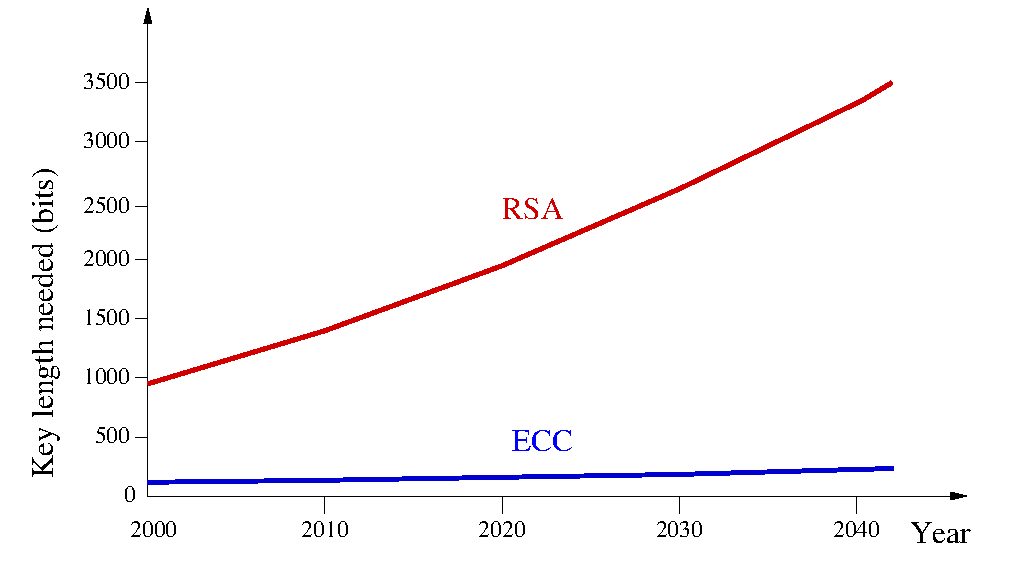
\includegraphics[scale=0.7]{figures/RSAKeyLength-2}
\caption{Prognosis of the key lengths to be regarded safe for RSA and
  Elliptic Curves\vspace{1ex}} 
\label{RSAKeylength}
\end{center}
\end{figure}

In addition, a digital signature can be processed 10-times faster with ECC
than with RSA.  However, verification of a given signature is still more
efficient with RSA than with ECC. Refer to
figure~\ref{ThousandBitMultiplications} (source: Dr.~J.\ Merkle, Elliptic
Curve Cryptography Workshop, 2001) for a comparison.  The reason is that
RSA public keys can be chosen relatively small as long as the secret key is
long enough.

% -> Figure 2
\begin{figure}[ht]
\begin{center}
\vspace{1.5cm}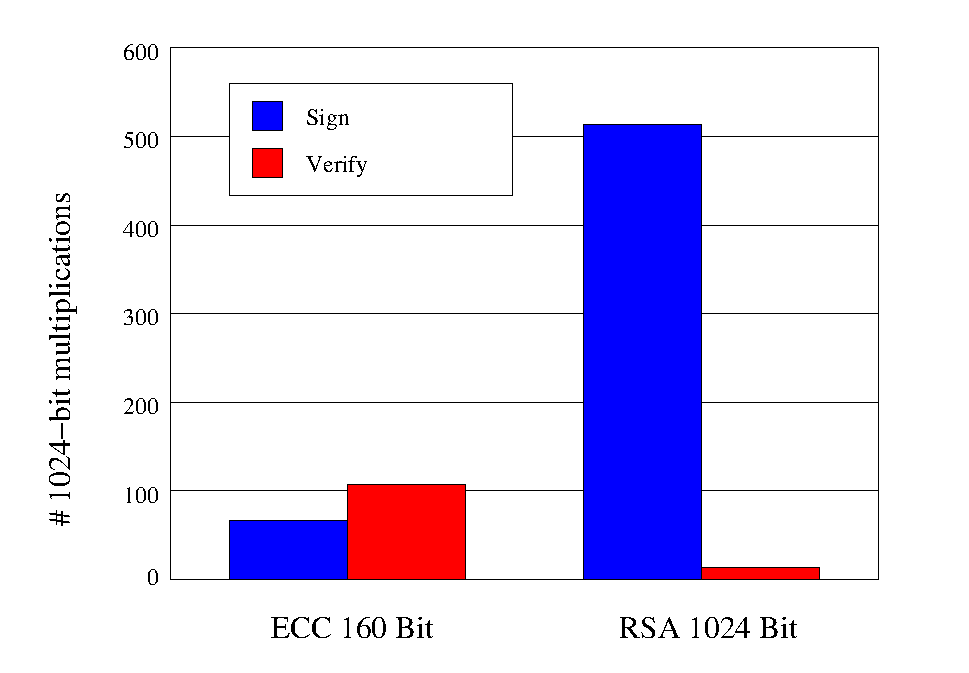
\includegraphics[scale=0.7]{figures/ECCRSA}
\caption{Comparison of signing and verification time for RSA and Elliptic Curves} 
\label{ThousandBitMultiplications}
\end{center}
\end{figure}

Nevertheless, thin clients like smart cards usually have to store the (long)
secret key and have to process a digital signature rather than verify one.
Therefore, there is a clear advantage in using ECC in terms of efficiency.
\par
\smallskip
Nowadays, the major problem with ECC implementations is the lack of standardization.
There is only one way to implement RSA, but there are many ways for ECC: One can work with
different sets of numbers, different (elliptic) curves --- described by parameters\footnote{%
see chapter \ref{ECC-Crypto}
} --- ,
and a variety of representations of the elements on the curve. Each choice has its
advantages and disadvantages, and one can certainly construct the most efficient for
each application. However, this causes problems in interoperability. But if all
ECC-tools should be able to communicate with each other, they will have to support
all different algorithms, which might put the advantage of efficient computation and
the need of less storage capacity to the contrary.

\begin{sloppypar}
Therefore, international standardization organizations like IEEE (P1363),
ASC (ANSI X9.62, X9.63), ISO/IEC as well as major players like RSA labs or
Certicom have recently started standardization initiatives. While the IEEE
only describes the different implementations, the ASC has explicitly stated
10 elliptic curves and recommends their usage. The advantage of the ASC
approach is that one needs only a single byte to indicate which curve is
meant. However, it is not yet clear whether the ASC curves will become a de
facto standard.
\end{sloppypar}

Although we see no need to replace RSA in any application today\footnote{%
Current information about the security of the RSA algorithm can be found in 
chapter \ref{SecurityRSA}.}, one should
take the usage of ECC-based tools into consideration whenever a new system
is set up --- in particular, when the tool should be available beyond 2005\footnote{%
Compare the recommendation of GISA: ``Fitting Crypto Algorithms'' from October 24th, 2002.
}.


\section{Elliptic curves -- history}

Mathematicians have been researching elliptic curves for over 100 years.
Over the course of time, many lengthy and mathematically complex results
have been found and published which are connected to elliptic curves. 
A mathematician would say that elliptic curves (or the mathematics behind
them) are widely understood. This research was originally purely 
mathematical. That is to say, elliptic curves were investigated, for 
example, in the mathematical areas of number theory and algebraic 
geometry, which are generally highly abstract. Even in the recent
past, elliptic curves played an important role in pure mathematics.
In 1993 and 1994, Andrew Wiles\index{Wiles, Andrew} published 
mathematical works that triggered enthusiasm far beyond the specialist
audience. In these works, he proved a conjecture put forward in the 1960's.
To put it short, this conjecture was concerned with the connection 
between elliptic curves and what are called module forms. What is
particularly interesting for most people is that the works of Wiles
also proved the famous second theorem of Fermat. Mathematicians had
spent centuries (Fermat lived from 1601 to 1665) trying to find a
strict proof of this theorem. Understandably, therefore, Wiles' proof
got a good response. Fermat formulated his theorem as follows 
(written in the border of a book):

\begin{quote} {\em
Cubum autem in duos cubos, aut quadratoquadratum in duos quadratoquadratos, et
generaliter nullam in infinitum ultra quadratum potestatem in duos ejusdem
nominis fas est dividere: cujus rei demonstrationem mirabilem sane detexi. Hanc
marginis exiguitas non caperet.
} \end{quote}

With a free translation, using the denotation of modern mathematics, this means: \\
No positive whole numbers $x, y$ and $z$ greater than zero exist such that $x^n +y^n = z^n$ for $n>2$. I have found an amazing proof of this fact, but there is
too little space within the confines of this book to include it.

This is truly amazing: A statement that is relatively simple to understand (we
are referring to Fermat's second theorem here) could only be proved after such a
long period of time, although Fermat himself claimed to have found a proof.
What's more, the proof found by Wiles is extremely extensive (all of Wiles
publications connected with the proof made up a book in themselves). This should
therefore make it obvious that elliptic curves are generally based on highly
complex mathematics.

Anyway that's enough about the role of elliptic curves in pure mathematics. 
In 1985 Neal Koblitz\index{Koblitz, Neal} and Victor Miller\index{Miller, Victor}
independently suggested using elliptic curves in cryptography. Elliptic 
curves have thus also found a concrete practical application. 
Another interesting area of application for elliptic curves is for
factorizing whole numbers \index{Factorization} (the RSA cryptographic system
is based on the \index{Complexity} difficulty/complexity of finding prime
factors of an extremely large number;  compare section \ref{SecurityRSA}.).
In this area, procedures based on elliptic curves have been investigated and
used since 1987 (compare section \ref{ECC-Factorization}). \\
There are also prime number tests\index{Prime number!test} based on elliptic
curves.
% (s. Anmerkung U. Kuehn)

Elliptic curves are used differently in the various areas. Encryption
procedures based on elliptic curves are based on the difficulty of a problem
known as elliptic curve discrete logarithm\index{Logarithm problem!discrete}.
The factorization of whole numbers uses the fact that a large number of
elliptic curves can be generated for a natural composite number $n$ with
several prime factors; however, these curves are not then groups for composite
$n$. More information about this can be found under the chapter \ref{ECC-Factorization}.

\section{Elliptic curves -- mathematical basics}

This section provides information about \index{Group} {\em groups} and
\index{Field} {\em fields}.

\subsection{Groups}

Because the term {\em group} is used differently in everyday language than in
mathematics, we will, for reasons of completeness, begin by introducing the
essential statement of the formal definition of a group:
\begin{itemize}
   \item A group is a non-empty set $G$ on which an operation ``$\cdot$''. The set $G$ is closed under this operation, which means that for any two elements $a, b$ taken from $G$, performing the operation on them gives an element in $G$, i.e. $ab=a\cdot b$ lies in $G$.
   \item For all elements $a, b$ and $c$ in $G$: $(ab)c = a(bc)$ (associative law).
   \item There exists an element $e$ in $G$ that behaves neutrally with respect
to the operation $\cdot$. That means that for all a in the set $G: ~ae = ea = a$.
   \item For each element $a$ in $G$ there exists a so-called inverse\footnote{The inverse is uniquely determined because if $x,y\in G$ are each inverse to $a$, i.e. $ax=xa=e$ and $ay=ya=e$, then $x=xe=x(ay)=(xa)y=ey=y$.} element $a^{-1}$ in $G$ such that: $aa^{-1} = a^{-1}a = e$.
\end{itemize}
If also $ab = ba$ (commutative law) for all $a, b$ in $G$, then we call the group an {\em Abelian} group.

Since we may define different operations on the same set, we distinguish them by giving them different names (e.g.\ $+$ addition or $\cdot$ multiplication).

The simplest example of an (Abelian) group is the group of whole numbers under
the standard operation of addition. The set of whole numbers is denoted as
${\mathbb Z}$. ${\mathbb Z}$ has an infinite number of elements, because
${\mathbb Z} = \{ \cdots, -4, -3, -2, -1, 0, 1, 2, 3, 4, \cdots\}$. For example, the
operation of $1+2$ lies in ${\mathbb Z}$, for $1+2 = 3$ and $3$ lies in
${\mathbb Z}$. The neutral element in the group ${\mathbb Z}$ is $0$. The
inverse element of $3$ is $-3$, for $3+(-3) = 0$.

For our purpose, so-called {\em finite} groups play an important role. This means that these exists a set
$\mathcal{M}$ with a fixed number of elements and an operation $+$ such that the
above conditions are fulfilled. One example of this is any set ${\mathbb Z}_n$
where ${\mathbb Z}_n = \{0, 1, 2, 3, \cdots, n-1\}, n$ is a positive whole number
and the operation is addition mod $n$, i.e. $a$ and $b$ in ${\mathbb Z}_n$ are
subject to the operation $a+b \;{\rm mod~} n$.

\paragraph{Cyclic groups}\index{Group!cyclic}
Cyclic groups\footnote{Cyclic groups can be in general also endless like the additive group of the integer numbers. We consider here only finite cyclic groups.} are those groups $G'$ that possess an element $g$
from which the group operation can be used to generate all other
elements in the group. This means that for each element $a$ in
$G'$ there exists a positive whole number $i$ such that if $g$ is
subject to the operation $i$ times (i.e. ``$g\cdot i$''),
$g+g+\cdots+g = a$ (additive group) or $g^i = g\cdot g \cdots g = a$
(multiplicative group). The element $g$ is the {\em generator} of
the cyclic group --- each element in $G'$ can be generated using
$g$ and the operation.

\paragraph{Group order}
Now to the order of an element of the group: Let $a$ be in $G$. The smallest
positive whole number $r$ for which $a$ subject to the operation with itself $r$
times is the neutral element of the group $G'$ (i.e.: $r \cdot a = a+a+\cdots+a =
e$ respectively $a^r = e$), is called the {\em order} of $a$.

The order of the group is the number of elements in the set $G$.

\subsection{Fields}

In mathematics, one is often interested in sets on which at least two (group) operations are defined --- frequently called addition and multiplication. Most prominent are so called fields.

A field is understood to be a set $K$ with two operations
(denoted as $+$ and $\cdot$) which fulfils the following conditions:
\begin{itemize}
   \item The set $K$ forms an Abelian group together with the operation $+$
(addition), where $0$ is the neutral element of the operation $+$.
   \item The set $K\setminus\{ 0\}$ also forms an Abelian group
together with the operation $\cdot$ (multiplication).
   \item For all elements $a, b$ and $c$ in $K$, we have $c\cdot (a+b) = c \cdot a + c
\cdot b$ and $(a+b) \cdot c = a \cdot c + b \cdot c$ (distributive law).
\end{itemize}

Fields may contain an infinite number of elements (e.g.\ the field of real numbers). They are called {\em infinite} fields. In contrast we call a field
{\em finite}, if it contains only a finite number of elements (e.g.\ ${\mathbb Z}_p = \{0, 1, 2, 3, \cdots, p-1\}$
, where $p$ is a prime. ${\mathbb Z}_p$ with addition mod $p$ and multiplication
mod $p$).
\index{Field!characteristic}
\paragraph{Characteristic of a field}
Let $K$ be a field and $1$ be the neutral element of $K$ with
respect to the multiplicative operation ``$\cdot$''. Then the characteristic of $K$ is said to be the order of $1$ with respect to the additive operation. This means that the characteristic of $K$ is the smallest positive integer $n$ such that
$$ \underbrace{1+1+\dots+1}_{\hbox{$n$ times}} =0 .
$$
If there is no such $n$, i.e. if $1+1+\dots+1\ne 0$ no matter how many $1$s we add, then we call $K$ a field
with characteristic $0$.

Thus, fields with characteristic $0$ are infinite since they contain the (pairwise distinct) elements $1$, $1+1$, $1+1+1$, \dots. On the other hand, fields with finite characteristic may by finite or infinite.

If the characteristic is finite, it has to be prime. This fact can easily be proved: Assume $n=pq$, $p,q<n$, is the characteristic of a field $K$. By definition of $n$, the elements $\bar p=\underbrace{1+1+\dots+1}_{\hbox{$p$ times}}$, $\bar q=\underbrace{1+1+\dots+1}_{\hbox{$q$ times}}$ of $K$ are not equal to $0$. Thus, there exist inverse elements $\bar p^{-1},\bar q^{-1}$ with respect to multiplication. It follows that $(\bar p\bar q)(\bar p^{-1}\bar q^{-1})=1$, which contradicts the fact that $\bar p\bar q=\bar n=\underbrace{1+1+\dots+1}_{\hbox{$n$ times}}=0$ and, hence, $\underbrace{(\bar p\bar q)}_{=0}(\bar p^{-1}\bar q^{-1})=0$.

\begin{remark}{:}\\
The field of real numbers has the characteristic $0$; the field ${\mathbb Z}_p$ has
the characteristic $p$. If $p$ is not prime, ${\mathbb Z}_p$ is not a field at all.
\end{remark}

The most simple field is ${\mathbb Z}_2=\{ 0,1\}$. It contains only two elements, the neutral elements with respect to addition and multiplication. In particular, we have $0+0=0$, $0+1=1+0=1$, $1+1=0$, $1\cdot 1=1$, $0\cdot 0=0\cdot 1=1\cdot 0=0$.

\index{Field!finite}
\paragraph{Finite Fields}
As mentioned above, each finite field has a characteristic $p\ne 0$, where $p$ is a prime. On the other hand, given a prime $p$ there is a field which has exactly $p$ elements, that is ${\mathbb Z}_p$.

However, the number of elements of a field need not be prime in general. For example, it is not hard to construct a field with $4$ elements\footnote{%
The set $K=\{0,1,a,b\}$ fitted with the operation defined in the tabular below is a field:\\
$
\begin{array}{|c||c|c|c|c|} 
\hline 
+ & 0 & 1 & a & b \\
\hline \hline
0 & 0 & 1 & a & b \\
\hline 
1 & 1 & 0 & b & a \\
\hline 
a & a & b & 0 & 1 \\
\hline 
b & b & a & 1 & 0 \\
\hline 
\end{array} \qquad {\rm ~und~} \qquad
\begin{array}{|c||c|c|c|c|} 
\hline 
\cdot & 0 & 1 & a & b  \\
\hline \hline
0 & 0 & 0 & 0 & 0 \\ 
\hline 
1 & 0 & 1 & a & b \\ 
\hline 
a & 0 & a & b & 1 \\ 
\hline 
b & 0 & b & 1 & a \\
\hline 
\end{array} 
$  \\
}.

One can show that the order of any field is a prime power (i.e. the power of a prime number). On the other hand, we can construct a field with $p^n$ elements for any given prime $p$ and positive integer $n$. Since two fields that have the same number of elements can not be distinguished\footnote{If $K,K'$ are fields with $k=p^n$ elements, then there is a one-to-one map $\varphi:K\to K'$, that respects the arithmetic of the field. Such a map is called an isomorphy. Isomorphic fields mathematically behave in the same way so that   it makes no sense to distinguish between them. For example, ${\mathbb Z}_2$ und $K'=\{ ZERO,ONE\}$ with zero-element $ZERO$ and one-element $ONE$ are isomorphic. We note that mathematical objects are only defined by their mathematical properties.}, we say that there is {\bf the field with $p^n$ elements} and denote it by $GF(p^n)$. Here $GF$ stands for {\it Galois Field} to commemorate the French Mathematician Galois.

The fields $GF(p)$ of prime order play a prominent role. They are called prime fields and often denoted by ${\mathbb Z}_p$\footnote{For prime fields additive as well as multiplicative group are cyclic. Furthermore, each field $GF(p^n)$ contains a subfield that is isomorphic to the prime field ${\mathbb Z}_p$.}.



% -----------------------------------------------------------------------------
\section{Elliptic curves in cryptography}\label{ECC-Crypto}

In cryptography elliptic curve are a useful tool. Such curves are described by some equation. A detailed analysis has shown that curves of the form\footnote{This curve is given by the zeros of a {\it polynomial}\index{Polynomial} $F$ of degree three in three variables. In general, expressions of the form
$P=\sum_{i_1,\dots,i_n\in\N_0} a_{i_1\dots i_n} x_1^{i_1}\dots x_n^{i_n}$ with coefficients $a_{i_1\dots i_n}\in K$ are called polynomials in $n$ variables $x_1,\dots,x_n$ with underlying field $K$, if ${\rm deg\,} P:=\max\{i_1+\dots +i_n: a_{i_1\dots i_n}\ne 0\}$ is finite, i.e. the sum has only finitely many non-zero terms (monomials). The sum of the exponents of the variables of each term of the sum is at most $3$, at least one term of the sum has a single variable with $3$ as value of the according exponent.}
\begin{equation}
 F(x_1,x_2,x_3)=-x_1^3+x_2^2x_3+a_1x_1x_2x_3-a_2x_1^2x_3+a_3x_2x_3^2-a_4x_1x_3^2-a_6x_3^3=0,
\label{eccbasisgleichung}
\end{equation}
are especially useful. The variables $x_1,x_2,x_3$ and parameters $a_1,\dots,a_4,a_6$ are elements of a given field $K$, which has certain properties that are make it useful from the cryptographic point of view. The underlying field $K$ might be the well known field of real numbers or some finite field (see last section).
In order to obtain a cure that is useful for cryptography, the parameters have to be chosen in a way that the following conditions hold
$$ \frac{\partial F}{\partial x_1}\ne 0, \quad \frac{\partial F}{\partial x_2}\ne 0, \quad
\frac{\partial F}{\partial x_3}\ne 0 .
$$
We identify points on the curve that can be derived from each over by multiplying each component with some scalar. This makes sense since $(x_1,x_2,x_3)$ solves (\ref{eccbasisgleichung}) if and only if $\alpha (x_1,x_2,x_3)$ ($\alpha\ne 0$) does. Formally, this means that we consider classes of equivalent points instead of single points, where points are called equivalent if one is the scalar multiple of the other one.
\\ If we put $x_3=0$ in the basic equation (\ref{eccbasisgleichung}), then this equation collapses to $-x_1^3=0$, leading to $x_1=0$. Thus, the equivalence class which includes the element $(0,1,0)$ is the only one that contains a point with $x_3=0$. For all points on the curve that are not equivalent to $(0,1,0)$, we may apply the following transformation
$$ K\times K\times (K\setminus\{0\})\ni (x_1,x_2,x_3) \mapsto (x,y):=\left( \frac{x_1}{x_3}, \frac{x_2}{x_3}\right) \in K\times K \, ,
$$
which reduces the number of variables to two instead of three. We note that the
basic equation (\ref{eccbasisgleichung}) $F(x_1,x_2,x_3)=0$  was chosen in a
way that this transformation leads to the famous so-called
Weierstrass-Equation\footnote{Karl Weierstrass\index{Weierstrass, Karl}, 31.10.1815$-$19.12.1897, German
mathematician, famous for his rigorous formal approach to mathematics.} holds
\begin{equation}
 y^2+a_1xy+a_3y = x^3+a_2x^2+a_4x+a_6 \, .
\label{ell}
\end{equation}
Since all but one point (i.e. equivalence class) of the elliptic curve can be described using equation (\ref{ell}), this equation is often called the elliptic equation, and its solutions written as
$$ {\bf E} = \left\{(x,y)\in K\times K \, |\, y^2+a_1xy+a_3y = x^3+a_2x^2+a_4x+a_6  \right\} \cup \{{\cal O} \}.
$$
Here, ${\cal O}$ represents the point $(0,1,0)$ that is loosely speaking mapped to infinity by the transformation (division by $x_3$) that reduces the three variables to two.

\begin{figure}[ht]
\begin{center}
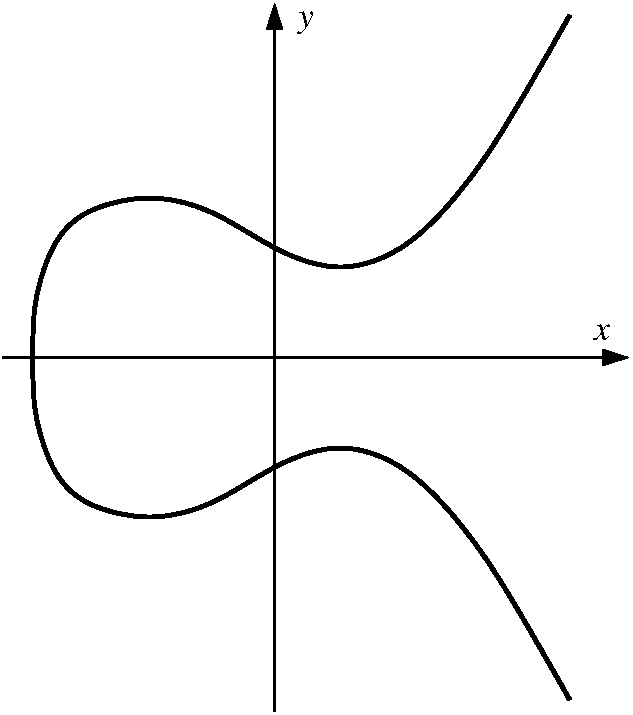
\includegraphics[scale=0.60]{figures/elliptic-curve}
\caption{Example of an elliptic curve with the real numbers as underlying field.\vspace{1ex}} 
\label{ExampleEllipticCurve}
\end{center}
\vskip -10 pt
\end{figure}

In contrast to figure \ref{ExampleEllipticCurve} only finite fields $K=GF(p^n)$ are used in elliptic curve cryptography. The reason is loosely speaking that in modern communication engineering data processing is always based on discrete data (simply because computers accept only discrete data).

For practical reasons, it turned out to be useful to take either $GF(p)$ with a large prime $p$ or $GF(2^n)$ with a (large) positive integer $n$. Using $GF(p)$ has the advantage of providing a relatively simple arithmetic; on the other hand $GF(2^n)$ allows a binary representation of each element that supports the way computers work. Other fields like, for example, $GF(7^n)$ do not have any of these advantages and are, thus, not considered, although there is no mathematical reason why they should not.

A coordinate transformation can result in a simpler version\footnote{Such a coordinate transformation is combination of a rotation and a dilatation of the coordinate system without changing the elliptic curve itself.} of the Weierstrass equation\index{Weierstrass, Karl}. Depending whether $p>3$, different transformations are used, and we obtain
\begin{itemize}
\item in case of $GF(p)$, $p>3$, the elliptic curve equation of the form
\begin{equation}
 y^2 = x^3 + ax + b
\label{ellp}
\end{equation}
with $4a^3+27b^2\ne 0$
\item in case of $GF(2^n)$ the elliptic curve equation of the form 
\begin{equation}
 y^2+xy = x^3 + ax^2 + b
\label{ell2}
\end{equation}
with $b\ne 0$\footnote{The form (\ref{ellp}) is called the standard form of the Weierstrass-equation\index{Weierstrass, Karl}. If the characteristic of the field is $2$ or $3$, we obtain $4=0$ respectively $27=0$, which means that the condition on parameters $a,b$ collapse. Loosely speaking, this is the reason why the transformation to the standard form does not work in these cases.}.
\end{itemize}
This conditions on the parameters $a,b$ ensure that the elliptic equation can be used in the context of cryptography\footnote{Formally we call such curves non singular.}.

Let $|E|$ denote the number of elements of an elliptic curve $E$ given an underlying field $GF(k)$ (for practical reasons either $k=p$ with $p$ prim or $k=2^n$). Then Hasse's theorem\cite{ec:Silverman1986} yields $| \, |E| - k-1\,| \le 2\cdot \sqrt{k}$. This Inequality is equivalent to $k+1 - 2\sqrt{k} < |E| < k+1+2\sqrt{k}$. In particular, this means that the number of elements of an elliptic curve is approximately $k$ (for large $k$). 

% -----------------------------------------------------------------------------
\section{Operating on the elliptic curve}

In order to work with elliptic curves in practice, we define an operation (often written in an additive way $+$) on the set of points on the curve. If we have a curve over the field $GF(p)$, we define the commutative operation $+$ by
\begin{enumerate}
\item $P+{\cal O}={\cal O}+P=P$ for all $P\in E$,
\item for $P=(x,y)$ and $Q=(x,-y)$ we set $P+Q={\cal O}$,
\item for $P_1=(x_1,x_2),P_2=(x_2,y_2)\in E$ with $P_1,P_2\ne {\cal O}$ and $(x_2,y_2)\ne (x_1,-y_1)$ we set $P_3:=P_1+P_2$, $P_3=(x_3,y_3)$ defined by
$$ x_3:=-x_1-x_2+\lambda^2 \, , \qquad y_3:=-y_1+\lambda (x_1-x_3)
$$
with the auxiliary quotient
$$ \lambda:=\left\{ \begin{array}{cl} \frac{y_1-y_2}{x_1-x_2} & {\rm if~} P_1\ne P_2, \\
                                     \frac{3x_1^2+a}{2y_1} & {\rm if~} P_1=P_2. \end{array} \right.
$$
\end{enumerate}
In particular, we obtain $-P=(x,-y)$ for $P=(x,y)\in E$.

If we deal with a curve over the field $GF(2^n)$, we define the operation $+$ in an analogous way by
\begin{enumerate}
\item $P+{\cal O}={\cal O}+P=P$ for all $P\in E$,
\item for $P=(x,y)$ and $Q=(x,x+y)$ we set $P+Q={\cal O}$,
\item for $P_1=(x_1,x_2),P_2=(x_2,y_2)\in E$ with $P_1,P_2\ne {\cal O}$ and $(x_2,y_2)\ne (x_1,x_1+y_1)$ we set $P_3:=P_1+P_2$, $P_3=(x_3,y_3)$ defined by
$$ x_3:=-x_1+x_2+\lambda+\lambda^2+a \, , \qquad y_3:=y_1+x_3+\lambda (x_1+x_3)
$$
with auxiliary quotient
$$ \lambda:=\left\{ \begin{array}{cl} \frac{y_1+y_2}{x_1+x_2} & {\rm if~} P_1\ne P_2, \\
                                   x_1+\frac{y_1}{x_1} & {\rm if~} P_1=P_2. \end{array}\right.
$$
\end{enumerate}
In particular, we obtain $-P=(x,-y)$ for $P=(x,y)\in E$.

(Note that $-(-P)=(x,x+(x+y))=(x,2x+y)=(x,y)$, since the underlying field
has characteristic $2$.)\footnote{An animation of the addition of points
on elliptic curves can be found on the Certicom\index{Certicom} homepage \\
\url{http://www.certicom.com/resources/ecc_tutorial/ecc_tutorial.html}}

One can verify that $+$ defines a group operation on the set $E\cap\{\cal O\}$.
In particular this means that the sum of two points is again a point on the
elliptic curve. How his operation works is geometrically visualized in the
following section.

% \newpage
\begin{figure}[htbp]
\subsection*{How to add points on an elliptic curve}
The following figures show how points on an elliptic curve over the field of real numbers are summed up using affine coordinates.
We note that the point infinity ${\cal O}$ cannot be shown in the affine plane.  
\begin{center}
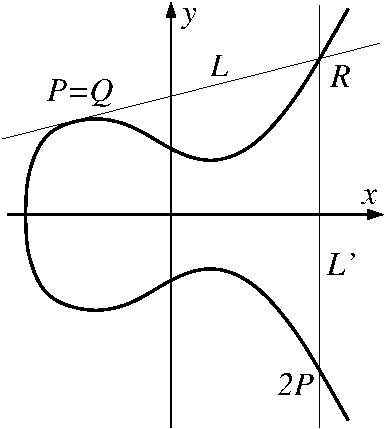
\includegraphics[scale=1.08]{figures/ec-mult2}
\caption{Doubling of a point} 
\vspace{\floatsep}
\vskip +20 pt
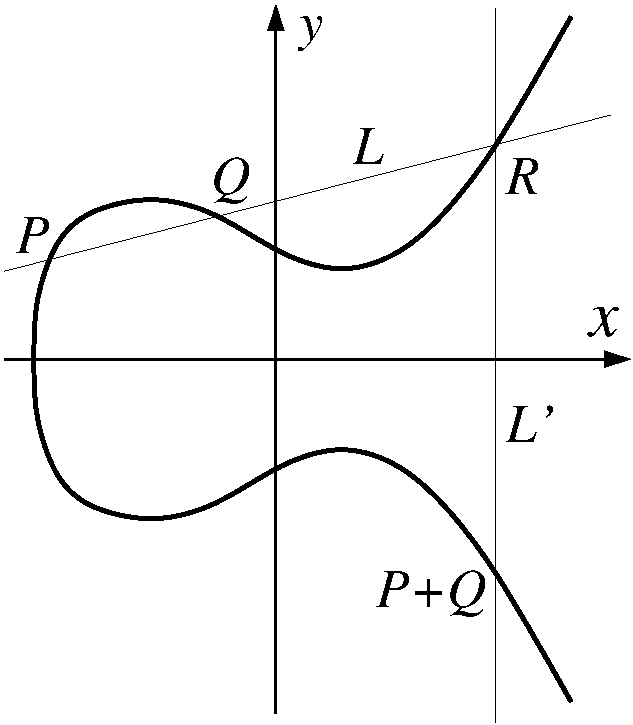
\includegraphics[scale=0.65]{figures/ec-add}
\caption{Summing up two different points over the real number field} % \footnotemark }
\end{center}
\end{figure}
\enlargethispage{+20pt}
\newpage


% -----------------------------------------------------------------------------
\section{Security of elliptic-curve-cryptography: The ECDLP}

As mentioned above in section \ref{ECC-Crypto}, we only consider elliptic curves over the finite\footnote{Discrete in contrast to continuous.} fields $GF(2^n)$ or $GF(p)$ (for a large prime $p$). This means that all parameters that describe the curve are taken from this underlying field. If $E$ is an elliptic curve over such a field and $P$ is a point on the curve $E$, then we can derive for all positive integers $m$
$$ mP := \underbrace{P+P+\dots+P}_{\hbox{$m$ times}} \, .
$$
Looking on this operation from the cryptographic point of view, it turns out to be very interesting by the following reason: On the one hand one needs only $\log m$ operations to calculate $mP$ --- one simply has to calculate $P$, $2P$, $2^2P$, $2^3P$, \dots, write $m$ in a binary form and finally add all these multiples $2^kP$ of $P$ with respect to the binary representation of $m$ --- on the other hand it seems to be very hard to find $m$ given $P$ and $Q=mP$ on $E$. Of course, we may simply calculate $P,2P,3P,4P,5P,\dots$ and compare each of them with $Q$. But this will take as much as $m$ operations.

Yet there is no algorithm known that efficiently derives $m$ given $P$ and $G$. The best algorithms known so far need about $\sqrt{q}$ operations where $q$ is the (largest) prime factor of $p-1$, in case the underlying field is $GF(p)$; here $m$ should be between $1$ and $q$ liegen so that one needs at most $\log q$ operations to calculate $mP$. However, the quotient $\frac{\sqrt{q}}{\log q}$ tends to $+\infty$ very fast for large $q$.

If we choose the parameters sufficiently large (for example, let $p$ be prime and at least $160$ bits long), an computer will easily be able to calculate $mP$ (in less than a second). The {\it inverse problem} however, to derive $m$ from $mP$ and $P$, can (still) not be solved in reasonable time.

This problem is known as the ``Elliptic Curve Discrete Logarithm Problem'' (for short ECDLP\index{ECDLP}).

\vskip +5 pt

In elliptic curve cryptography we formally look at points on the elliptic curve as elements of a group with point addition $+$ as operation. Furthermore, we use only elliptic curves that have a sufficiently large number of points. However, in special cases curves may be weak and not useful due to other reasons. For such special cases the ECDLP can be much easier to solve than in the general case. This means that one has to look carefully at the parameters when choosing an elliptic curve for cryptographic applications.

Not useful for cryptography are {\em a-normal} (that are curves over ${\mathbb Z}_p$,
for which the set ${\bf E}$ consists of exactly $p$ elements) and {\em supersingular} curves (that are curves, for which the ECDLP can be reduced to the ``normal'' discrete logarithms in another, smaller finite field). This means that there are cryptographically useful and non-useful elliptic curves. Given the parameters $a$ and $b$, it is possible to determine whether a curve is useful or not. In many publications one can find parameters that turned out to be useful for cryptography. The open (scientific) discussion guarantees that these results take into account latest research.
\vskip +5 pt

Given a secure curve, the time that is needed to solve the ECDLP is strongly correlated with parameter $p$ in case $GF(p)$ respectively $n$ in case of $GF(2^n)$. The larger these parameters become, the more time an attacker needs to solve the ECDLP --- at least with the best algorithms known so far. Experts recommend bit-lengths of $200$ for $p$ for secure curves. A comparison with RSA modulus length shows why elliptic curves are so interesting for applications. We note that the computation effort for signing and encryption is closely related to the bit-length of the parameters. In addition the initiation process, i.e. the generation of the private-public-key-pair, becomes more complicated the larger $p$ is. Thus, one looks for the smallest parameters that still come along with the security required. It is remarkable that a length of $200$ bits for $p$ is sufficient to construct a {\em good} elliptic curve that is as secure as RSA with a $1024$ bit \index{RSA!modulus} RSA modulus (as far as we know today). For short, the reason for this advantage of ECC lies in the fact that the best algorithms known for solving the ECDLP need exponential time while the best algorithms for factorizing are sub-exponential (number field sieve, quadratic sieve or factorizing with elliptic curves). Hence, the parameters for a cryptosystem that is based on the problem of {\em factorizing large integers} have to be larger than the parameters for a system based on ECDLP.


% -----------------------------------------------------------------------------
\section{Encryption and signing with elliptic curves}

\begin{sloppypar}
  The {\em elliptic curve discrete logarithm
    problem}\index{Problem of discrete logarithm} (ECDLP) \index{ECDLP} is the basis for elliptic curve cryptography. Based on this problem, there are different signature schemes. In order to apply one of these, we need:
\end{sloppypar}
\begin{itemize}
    \item An elliptic curve {\bf E} with an underlying field $GF(p^n)$.
    \item A prime $q\ne p$ and a point $G$ on the elliptic curve ${\bf E}$ with order $q$. This means that $qG={\cal O}$ and $rG\ne {\cal O}$ for all $r\in \{1,2,\dots,q-1\}$. Thus $q$ is a factor of the group order (i.e. the number of elements) $\#{\bf E}$ of $E$. Since $q$ is prime, $G$ generates a cyclic sub-group of ${\bf E}$ of order $q$.
\end{itemize}
The parameters mentioned are often called \index{Domain parameter}
{\em Domain} parameter. They describe the elliptic curve ${\bf E}$ and 
the cyclic sub-group of ${\bf E}$ on which the signature scheme is based.

\par
%\smallskip
%{\bf Encryption:}
\subsection{Encryption}

Using elliptic curves one can construct a key exchange protocol based on the Diffie-Hellman protocol \index{Diffie-Hellman} (see chapter \ref{DH-KeyExch}). The key exchanged can be used for a subsequent symmetric encryption. We note that in contrast to RSA there is no pair of private and public key that can be used for encryption and decryption!

In the notation of elliptic curves, the Diffie-Hellman protocol reads as follows: First both partners (A und B) agree on a group $G$ and an integer $q$. Then they choose $r_A,r_B\in\{1,2,\dots,q-1\}$ at random, derive the points $R_A=r_AG$, $R_B=r_BG$ on the elliptic curve and exchange them (using an insecure channel). After that A easily obtains $R=r_AR_B$; B gets the same point ($R=r_Ar_B G$) by calculating $r_BR_A=r_Br_AG=r_Ar_BG=R$. We note that $R_A,R_B$ are easy to derive as long as $r_A$ respectively $r_B$ are known $G$. However, the inverse operation, to get $R_A$ respectively $R_B$ from $r_A$ respectively $r_B$ is hard.
\\ Using the best algorithms known so far, it is impossible for any attacker to obtain $R$ without knowing either $r_A$ or $r_B$ --- otherwise he would have to solve the ECDLP.

In order to prohibit a ``Man-in-the-middle"{}~attack, one may sign the values $G,q,R_A,R_B$ as described in chapter \ref{Impersonalisierungsattacke}.


\par
%\smallskip 
%{\bf Signing:}
\subsection{Signing}

Using the \index{DSA} DSA signature scheme, one can proceed as follows: The signing party chooses a (non-trivial) number $s\in{\mathbb Z}_q$, which will be the private key, and publishes $q$, $G$ and $R=sG$. We note that $s$ cannot be obtained from $G$ and $R$ are not sufficient --- a fact on which the security of the signature scheme is based.

Given the message $m$, which should be signed, one first constructs a digital finger print using a hash-algorithm $h$ such that $h(m)$ has its values in $\{0,1,2,\dots, q-1\}$. Thus, $h(m)$ can be considered as an Element of ${\mathbb Z}_q$. Then the signing party chooses a random number $r\in{\mathbb Z}_q$ and derives $R=(r_1,r_2)=rG$. We note that the first component $r_1$ of $R$ is an element of $GF(p^n)$. This component will then be projected onto ${\mathbb Z}_q$, i.e. in case of $n=1$ it is interpreted as the remainder of an element of $\{0,1,\dots,p-1\}$ divided by $q$. This projection of $r_1$ onto ${\mathbb Z}_q$ is denoted by $\bar r_1$. Then one determines $x\in {\mathbb Z}_q$ such that
$$ rx-s\bar r_1-h(m)=0 .
$$
The triple $(m,r_1,x)$ is then published as the digital signature of message $m$.

\par
%\smallskip 
%{\bf Signature Verification:}
\subsection{Signature verification}

In order to verify a signature, one has to build $u_1=h(m)/x$, $u_2=\bar r_1/x$ (in ${\mathbb Z}_q$ and derive
$$ V=u_1G+u_2Q .
$$
Since we have $Q=sG$, the point $V=(v_1,v_2)$ satisfies $v_1=u_1+u_2s$. We note that this operations take place in the field $GF(p^n)$. The projection of $GF(p^n)$ on ${\mathbb Z}_q$ mentioned above should be chosen in such a way that $\bar v_1=u_1+u_2s$ is an element of ${\mathbb Z}_q$. Then it follows that
$$ \bar v_1=u_1+u_2s=h(m)/x+\bar r_1 s/x=(h(m)+\bar r_1s)/x=rx/x=r .
$$
Since $R=rG$, we obtain $\bar v_1=\bar r_1$, i.e. $R$ and $V$ coincide modulo the projection onto ${\mathbb Z}_q$.


% -----------------------------------------------------------------------------
\hypertarget{faktell}{}
\section{Factorization using elliptic curves} \label{ECC-Factorization}

There are factorization%
\footnote{Especially John M. Pollard \index{Pollard, John M.} was involved
in the development of many different factorization algorithms; also at
factorization with ECC he was one of the leading heads. As an employee
of British Telekom he never published much. At the RSA data Security Conference
in 1999 he was awarded for his ``outstanding contributions in mathematics'':
\href{http://www.eff.org/Privacy/Crypto_misc/DESCracker/HTML/19990118_rsa_awards.html}
{\texttt{http://www.eff.org/Privacy/Crypto\_misc/DESCracker/HTML/19990118\_rsa\_awards.html}}.
}
algorithms based on elliptic curves%
\footnote{In 1987 H.W. Lenstra published
a factorization algorithm, based on elliptic curves (see \cite{ec:Lenstra1987}).
The biggest compound number currently 
factorized\index{Factorization!factoring records} with elliptic curves is 
the number $ 628^{59}-1, $ which has 55 decimal digits. It was
found Oct. 6th, 2001 by M. Izumi 
(See \hyperlink{Lenstra2}{ECMNET}\index{ECMNET}).
}. 
More precisely, these procedures exploit the fact that elliptic curves can
be defined over ${\mathbb Z}_n$ ($n$ composite number). Elliptic curves 
over ${\mathbb Z}_n$ do not form a group, because not every point on such 
an elliptic curve has an inverse point. This is connected with the fact 
that - if $n$ is a composite
number - there exist elements in ${\mathbb Z}_n$ that do not have an inverse
with respect to multiplication mod $n$. In order to add two points on an
elliptic curve over ${\mathbb Z}_n$, we can calculate in the same way as on
elliptic curves over ${\mathbb Z}_p$. Addition of two points (on an elliptic
curve over ${\mathbb Z}_n$), however, fails if and only if a factor of $n$ has
been found. The reason for this is that the procedure for adding points on
elliptic curves gives elements in ${\mathbb Z}_n$ and calculates the inverse
elements for these (with respect to multiplication mod $n$) in ${\mathbb Z}_n$.
The extended \index{Euclidean algorithm} Euclidean algorithm is used here. If
the addition of two points (that lie of an elliptic curve over ${\mathbb Z}_n$)
gives an element in ${\mathbb Z}_n$ that does not have an inverse element in
${\mathbb Z}_n$, then the extended Euclidean algorithm delivers a genuine factor
of $n$.

Factorization using elliptic curves thus principally works as follows: 
Random curves over ${\mathbb Z}_n$ are selected, as well as random points
(that lie on this curve) and add them; you thus obtain points that also
lie on the curve or find a factor of $n$. 
Factorization algorithms based on elliptic curves
therefore work probabilistically. The opportunity of defining large number of
elliptic curves over ${\mathbb Z}_n$ allows you to increase the probability of
finding two points which you can add to obtain a factor of $n$. These procedures
are therefore highly suitable for parallelization.



% -----------------------------------------------------------------------------
\newpage
% \section{Implementing elliptic curves for educational purposes, pat\-ent aspects}
\section{Implementing elliptic curves for educational purposes}
\label{ec:Implementing-for-Education}

There are not many free programms offering ECC under a graphical user interface.
The following subsections explain which according functionality is available in
CrypTool and in Sage.


% -----------------------------------------------------------------------------
\subsection{CrypTool}

CrypTool offers elliptic curves for the digital signature function%
\footnote{%
The dialog box, which appears in CrypTool\index{CrypTool} after clicking the menu
{\bf Digital Signatures/PKI \textbackslash{} Sign Message},
offers the EC methods ECSP-DSA and ECSP-NR.

} and for ECC-AES hybrid encryption%
\footnote{%
Within CrypTool\index{CrypTool} you can find this technique using the menu
path {\bf Crypt \textbackslash{} Hybrid}.

}.

It implements the basic algorithms for group operations, for generating elliptic
curves, for importing and exporting parameters for elliptic curves over finite
fields with $p$ elements ($p$ prime). The algorithms have been implemented in
ANSI C and comply with draft no. 8 of the IEEE P1363 work group {\em Standard
Specifications for Public Key Cryptography}

{\url{http://grouper.ieee.org/groups/1363}}.

The procedure implements the cryptographic primitives for generating and
verifying signatures for the variations of Nyberg-Rueppel signatures and
\index{DSA} DSA signatures based on elliptic curves.


% -----------------------------------------------------------------------------
\subsection{Sage}
\label{ec:Sage_Massierer}
\index{Sage}
\index{Sage!Code examples}

In Sage elliptic curves are described at

\url{http://www.sagemath.org/doc/constructions/elliptic_curves.html}%
\footnote{%
According Sage samples can be found at the "Published Worksheets" at
\url{http://www.sagenb.org/pub/}\\
- about Elliptic Curve: \url{http://www.sagenb.org/home/pub/606/} \\
- about Elliptic Curve El Gamal: \url{http://www.sagenb.org/home/pub/104/}, or at

  \noindent\hangindent=6pt\makebox[6pt][l]{-}%
  the "Elliptic Curve Cryptography (ECC) Tutorial"\\
  \url{http://www.williamstein.org/simuw06/notes/notes/node12.html}

}.

\noindent Additionally there is an exhaustive, interactive
\hyperlink{ec:Web-Link:Sage_Massierer}{ECC tutorial} by Maike Massierer.
This interactive introduction to Elliptic Curve Cryptography is built up as
a Sage notebook.

Sage notebooks are running after a logon within a browser%
\footnote{%
If you installed Sage on your own (Unix) server, you first have to enter at the
command line the command \verb#notebook()#.

}${}^,$\footnote{%
The ECC notebook of Maike Massierer needs the KASH3 library: Therefore e.g.\ with Sage 4.2.1
the package ``kash3-2008-07-31.spkg'' has to be installed (command \verb#sage -i#).
}.

The ECC notebook\index{Elliptic curves!ECC notebook}\index{Massierer, Maike} of
Massierer\footnote{%
Instructions to use an interactive Sage notebook:\\

  \noindent\hangindent=6pt\makebox[6pt][l]{-}%
  Public Sage servers like \url{http://sage.mathematik.uni-siegen.de:8000} or
  \url{http://www.sagenb.org/} often offer running samples as "Published Worksheets",
  which you can run and download without login on. These worksheets are listed
  if you click on ``Published'' in the above right corner.

  \noindent\hangindent=6pt\makebox[6pt][l]{-}%
  Worksheets using the  \verb#interact# command currently need some additional
  todos for a user to work correctly: sign-in, make a copy and execute all
  commands again.\\
  This works as follows (described for the sagenb server and for the ECC tutorial):\\
 
  \noindent\hangindent=6pt\makebox[6pt][l]{-}%
  Sign-up for a Sage notebook account at \url{http://sagenb.org/register}
  and sign in at \url{http://sagenb.org/}.

  \noindent\hangindent=6pt\makebox[6pt][l]{-}%
  Open the worksheet \url{http://sagenb.org/home/pub/1126/}.
  This contains the table of contents of the interactive ECC notebook.
  From here you can navigate via a click to the different chapters of the document.

  \noindent\hangindent=6pt\makebox[6pt][l]{-}%
  In the very top left corner, click \verb#Edit a copy# in order to create
  your own copy of the worksheet.

  \noindent\hangindent=6pt\makebox[6pt][l]{-}%
  Sometimes it's necessary at the beginning to re-evaluate the worksheet.
  Click in the left upper corner on \verb#Action -> Evaluate all#.

  \noindent\hangindent=6pt\makebox[6pt][l]{-}%
  Some of the applications still do not always work after opening a worksheet.
  Instead of nice output, they show lots of (blue) error messages.
  This normally can be solved quickly by clicking the gray  ``\%hide'' string:
  Then you get the code behind the graphics. Simply generate the graphics
  again with Shift-Enter.\\
  Even after doing this, the graphics code does not always disappear. Instead,
  it sometimes turns gray. Should this happen, click on the gray text,
  then click somewhere outside of the text box. The code will then
  disappear and leave you with a nice layout of the worksheet.

  \noindent\hangindent=6pt\makebox[6pt][l]{-}%
  Some of the ECC tutorial's content uses a special math fonts that are
  not installed by default with most browsers. When you notice that
  formulas are not displayed correctly or even get an error message
  about missing fonts from your browser, you need to install the jsMath
  fonts for a better layout.\\
  See \url{http://www.math.union.edu/~dpvc/jsMath/}
  and \url{http://pubpages.unh.edu/~jsh3/jsMath/}.\\
  After installing these fonts you can see the jsMath symbol at the lower border
  of your browser. If you click this symbol you can find the download page for
  the TIFF fonts. This fonts installation has to be done at every PC.

  \noindent\hangindent=6pt\makebox[6pt][l]{-}%
  According to the Sage-support newsgroup there is work underway
  to create a system for using \verb#@interact# completely outside of the
  Sage notebook (JS code within a static html pages).

}${}^,$\footnote{%
  Since 2008 this ECC notebook can be found at
    \url{http://sage.mathematik.uni-siegen.de:8000/home/pub/45/} (\verb!#45 to #52!).
  To logon in Siegen you have to allow port 8000 and Cookies.\\
  Since 2009 an updated version of this ECC notebook can be found at
    \url{http://sagenb.org/home/pub/1126/} (\verb!#1126 to #1133!).
}
consists of 8 parts (title page plus 7 chapters)
% "Titelseite" mit Inhaltsverzeichnis plus 7 Kapitel
and aims to let even beginners understand what elliptic curves are:

\begin{enumerate}
   \setcounter{enumi}{-1}
   \item ECC Notebook (title page and contents)
   \item Introduction and Overview
   \item Motivation for the use of Elliptic Curves in Cryptography
   \item Elliptic Curves in Cryptography
   \item Cryptographic Protocols in ECC
   \item Domain Parameter Generation for ECC Systems
   \item Conclusion and Further Topics
   \item References

\end{enumerate}



% -----------------------------------------------------------------------------
\newpage
\section{Patent aspects}
\index{Patent}

If the field $GF(2^n)$ is used instead of the prime field $GF(p)$, one has to make substantial changes in the implementation. The advantage of $GF(2^n)$ lies in the fact that calculations in $GF(2^n)$ can be implemented very efficiently using the binary representation. In particular, divisions are much easier to process compared to $GF(p)$ (this is particularly important in the signature scheme mentioned above where a division is needed for processing a signature as well as for the verification).

In order to achieve maximal gain in efficiency, one may choose a field that allows special basis like polynomial basis (useful for software implementations) or normal basis (best for hardware implementations). For special $n$ (like, for example, $n=163,179,181$) one may even combine both advantages. However, they are still non-standard.

Sometimes only the first component and one additional bit is used as representation of a point on the elliptic curve instead of the full two components. Since the first component together with the additional bit is sufficient to derive the full point, this representation minimizes the memory capacity needed. In particular, for normal basis this point compression can be implemented efficiently. In addition, the cryptographic protocols themselves become more effective. A disadvantage is, however, that {\it point compression} can be used for about half of all elliptic curves only and is protected under
US patent (US Patent 6141420, Certicon), causing additional costs.
In the general case $GF(p^n)$ (and also in case $n=1$) often so called affine or projective co-ordinates are used. Depending on the application, these co-ordinates may result in a gain in efficiency as well.

A comprehensive description of all implementations and their advantages and disadvantages would go far beyond the scope of this paper. We only want to state that there is a variety of possible implementations for elliptic curve cryptography, much more than for RSA. Therefore, there are serious efforts to reduce this large to a small number of standard implementations. Some standardization committees even try to reduce the complexity by focusing on a small number of (prescribed) curves (ASC-approach).

Today it is still not clear whether these standardization initiatives will be
successful or not. However, without agreed standards, ECC is not likely to
become a real alternative for RSA. The committees might be forced to act fast
if there was a break-through in factorization.


% -----------------------------------------------------------------------------
\section{Elliptic curves in use}

Today elliptic curve cryptography is already in use. A prominent example is the
information network Bonn-Berlin\footnote{%
The Informationsverbund Bonn-Berlin (IVBB) connects governmental institutions
in the old and new German capital.\\
\url{http://www.cio.bund.de/cln_094/sid_92C19118CBA5A021AFD1ABAEC15D2B77/DE/IT-Angebot/IT-Infrastrukturen/IVBB/ivbb_inhalt.html}
                                        }\index{IVBB}, used for the exchange
of strictly confidential documents between different German federal governmental
institutions in Berlin and Bonn. With the help of ECC a high security solution
could be realized. Interoperability, however, played only a minor role.

In Austria ECC has been massively launched: A bank card with digital signature function.

Both examples show the typical range of application for elliptic curve cryptography: For high security solutions and for implementations on smartcards in which the key length is crucial (because of physical memory available).




%--------------------------------------------------------------------
\newpage
%\addcontentsline{toc}{subsection}{Literaturverzeichnis}
\begin{thebibliography}{99999}
\addcontentsline{toc}{section}{Bibliography}

    \bibitem[Cassels1991]{ec:Cassels1991} J. W. S. Cassels,
	\index{Cassels 1991} \\
        {\em Lectures on elliptic curves},\\
	Cambridge University Press, 1991, 143 pages.
    \bibitem[Koblitz1984]{ec:Koblitz1984}N. Koblitz, 
	\index{Koblitz 1984} \\
        {\em Introduction to elliptic curves and modular forms},\\
	Graduate Texts in Mathematics, Springer-Verlag, 1984.
    \bibitem[Koblitz1998]{ec:Koblitz1998}N. Koblitz,  
	\index{Koblitz 1998}\\
	{\em Algebraic aspects of Cryptography. With an appendix on 
	Hyperelleptic curves by Alfred J. Menezes, Yi Hong Wu and Robert 
	J. Zuccherato}, \\
	Springer-Verlag, 1998, 206 pages.
    \bibitem[Lenstra1987]{ec:Lenstra1987} H.W. Lenstra, 
        \index{Lenstra 1987} \\
        {\em Factoring integers with elliptic curves}, \\
	Annals of Mathematics 126, pp. 649-673, 1987.
    \bibitem[Lenstra1999]{ec:Lenstra1999} Arjen K. Lenstra, Eric R. Verheul
        \index{Lenstra/Verheul 1999} \\
        {\em Selecting Cryptographic Key Sizes (1999)},\\
	Journal of Cryptology: the journal of the International 
	Association for Cryptologic Research \\
	\href{http://www.cryptosavvy.com/cryptosizes.pdf}
	{\texttt{http://www.cryptosavvy.com/cryptosizes.pdf}}
    \bibitem[Menezes1993]{ec:Menezes1993}A. J. Menezes, 
	\index{Menezes 1993} \\
        {\em Elliptic curve public key cryptosystems},\\
	Kluwer Academic Publishers, 1993.
    \bibitem[Silverman1986]{ec:Silverman1986} J. Silverman, 
        \index{Silverman 1986}\\
        {\em The Arithmetic of Elliptic Curves},\\
	Springer-Verlag, 1986.
    \bibitem[Silverman1992]{ec:Silverman1992}J. Silverman,
	\index{Silverman 1992} \\
        {\em The arithmetic of elliptc curves},\\
	Graduate Texts in Mathematics, Springer-Verlag, 1992.
    \bibitem[SilvermanTate1992]{ec:SilvermanTate1992}J. Silverman, J. Tate,
	\index{Silverman/Tate 1992} \\
        {\em Rational points on elliptic curves},\\
	Springer-Verlag, 1992.

\end{thebibliography}



%--------------------------------------------------------------------
\chapter*{Web links}
\addcontentsline{toc}{section}{Web links}

\begin{enumerate}

        \hypertarget{ec:Web-Link:Sage_Massierer}{} 
   \item Interactive introduction to elliptic curves and elliptic curve cryptography
        with Sage\index{Sage} by Maike Massierer and the CrypTool team,\\
        \url{http://sagenb.org/home/pub/1126/} (\verb!#1126 to #1133!) \\
        ECC Tutorial as Sage Notebook \\
        Version 1.2, November 2009

   \item Certicom Online Tutorial\index{Certicom},\\
        \url{http://www.certicom.com/resources/ecc_tutorial/ecc_tutorial.html}      
		
   \item Working group IEEE P1363, \\
        \url{http://grouper.ieee.org/groups/1363}

   \item \hypertarget{Lenstra2}{}
        An informative web page about factorization with elliptic curves, \\
        \url{http://www.loria.fr/~zimmerma/records/ecmnet.html}\\
        It contains literature related to the topic factorization with 
	elliptic curves as well as links to other web page. 

   \item Key length comparison by Arjen Lenstra and Eric Verheul,\\
        \url{http://cryptosavvy.com/table.htm}

\end{enumerate}


% Local Variables:
% TeX-master: "../script-en.tex"
% End:


\renewcommand{\CTBChapName}{(Chap BitCiphers)}    % $Id: cryptomethods.tex 3712 2016-03-22 23:36:46Z xesslinger $
% !Mode:: "TeX:DE"    % Setting document mode and submode for WinEdt
% ..............................................................................
% B i t b l o c k -  u n d  B i t s t r o m - V e r s c h l ü s s e l u n g
% ~~~~~~~~~~~~~~~~~~~~~~~~~~~~~~~~~~~~~~~~~~~~~~~~~~~~~~~~~~~~~~~~~~~~~~~~~~~~~~

\begin{refsegment}


%BERM0 Changed when bc becoming part of the CT book.
%BERM1 Transformed to comment when bc becoming part of the CT book: There it already was in script-en.tex.
%BERM2 Transformed to comment when bc becoming part of the CT book: Added there to script-en.tex.
%BERM3 Redefined new commands already existing in moderncryptography.tex when bc becoming part of the CT book
%BERM3 (see http://tex.stackexchange.com/questions/36175/what-do-newcommand-renewcommand-and-providecommand-do-and-how-do-they-differ).

%BERM1 \documentclass[11pt,a4paper,leqno]{report}
%BERM1 \usepackage[latin1]{inputenc}
%BERM1 \usepackage[T1]{fontenc}
%BERM1 \usepackage{german}
%BERM1 \usepackage{amsmath,amssymb,amscd,latexsym}
%BERM1 \usepackage{color}
%BERM1 \usepackage{hyperref}
%BERM1 \usepackage{makeidx}
%BERM1 \usepackage[pdftex]{graphicx}
%BERM1 \usepackage{float}

% ++++++++++++++++++++++++++++++++++++++++++++++++++++++++++++++++++++++++++
% Pommerenings Spezialitäten
% ~~~~~~~~~~~~~~~~~~~~~~~~~~~~~~~~~~~~~~~~~~~~~~~~~~~~~~~~~~~~~~~~~~~~~~~~~~
\newcommand*{\F}{\mathbb{F}}
\newcommand*{\M}{\mathbb{M}}

%\newcommand*{\C}{\mathbb{C}}
\newcommand*{\N}{\mathbb{N}}
\newcommand*{\Q}{\mathbb{Q}}
\newcommand*{\R}{\mathbb{R}}
\newcommand*{\Z}{\mathbb{Z}}

\newcommand*{\lsb}{\operatorname{lsb}}
\newcommand*{\Oh}{\operatorname{O}}

% ++++++++++++++++++++++++++++++++++++++++++++++++++++++++++++++++++++++++++
% CrypTool-Spezialitäten
% ~~~~~~~~~~~~~~~~~~~~~~~~~~~~~~~~~~~~~~~~~~~~~~~~~~~~~~~~~~~~~~~~~~~~~~~~~~
%BERM1 \newtheorem{definition}{Definition}[section]
%BERM1 \newtheorem{satz}{Satz}[section]
%BERM1 \newenvironment{Beweis}[1]{\noindent\textbf{Beweis #1} \\}{\hfill$\Box$\par}
%BERM1 \newenvironment{example}[1]{\noindent\textbf{Beispiel#1}}{}
%BERM1 \newenvironment{remark}[1]{\noindent\textbf{Bemerkung#1}}{}
%BERM1 \setcounter{secnumdepth}{4} % Nummerierung auch bei subsubsection
%BERM1 \floatstyle{ruled}
%BERM1 \newfloat{sagecode}{!ht}{loc}[chapter]
%BERM1 \floatname{sagecode}{SageMath-Beispiel}

\sloppy
\frenchspacing
%BERM1 \makeindex
%BERM1 \begin{document}

%BERM0 \setcounter{chapter}{98}  % ====> Dummy - beim Einfügen ins CT-Skript löschen <=====
\setcounter{satz}{0}
\setcounter{definition}{0}


\newpage %BERM0
\hypertarget{Chapter_BitCiphers}{}   %BERM0
\chapter{Einführung in die Bitblock- und Bitstrom-Verschlüsselung}
\chaptermark{Einführung Bit-Verschlüsselung}
\label{Chapter_BitCiphers}
(\hyperlink{author_Klaus-Pommerening}{Klaus Pommerening},
 Januar--Juni 2015; Updates: Jan. 2016, Apr. 2016) \\

\noindent
Während asymmetrische Verschlüsselung meistens zahlentheoretische Methoden
verwendet, beruhen die heutigen symmetrischen
Verschlüsselungsverfahren\index{Verschlüsselung!symmetrisch}
in der Regel auf Boolescher Algebra\index{Boolesche Algebra}\index{Algebra!Boolesche},
d.\,h., auf Manipulationen von Bits.
Das ist eine ganz andere Art von Mathematik, für Einsteiger vielleicht
ungewohnt, so dass dieses Kapitel eine sanfte Einführung in dieses mathematische
Gebiet sein soll. Vorkenntnisse aus einem Grundkurs Mathematik am Gymnasium
sollen ausreichen. Ohne weitere Erklärung als bekannt
angenommen werden die Begriffe "`Variable"' und "`Funktion"', auch für Argumente
und Werte in anderen Mengen als den reellen Zahlen.

Beginnen wir also mit der Beschreibung, wie Bits interpretiert, verknüpft
und durch Funktionen, sogenannte Boolesche
Funktionen\index{Boolesche Funktion}\index{Funktion!Boolesche}, verarbeitet werden.
Namenspatron dieses Fachgebiets ist
George Boole\index{Boole, George}\footnote{%
  George Boole, englischer Mathematiker, Logiker und Philosoph,
  2.11.1815--8.12.1864.
},
der durch die Einführung der elementaren logischen Operationen die Logik
mathematisch formalisierte ("`Logikkalkül\index{Logikkalkül}"').
Moderne symmetrische Verschlüsselungsverfahren, wie auch
Hash-Funktionen\index{Hashfunktion},
werden durch Systeme von Booleschen Funktionen beschrieben.

Der Schwerpunkt dieses Kapitels liegt in der Einführung in die
mathematischen Grundlagen der Verschlüsselungstechniken, die auf
Bits operieren. Konkrete Verfahren werden nicht detailliert beschrieben;
hierfür sei auf die Bücher von
Menezes/Orschot/Vanstone \cite{Menezes2001},
Oppliger \cite{Oppliger2011},
Paar und Pelzl \cite{PaPe2009},
Schmeh \cite{Schm2003, Schm2016}
und Stamp \cite{Stamp2007} verwiesen.

Noch ein Wort zur Nomenklatur: Die Verfahren werden in der Literatur
meist als "`Blockchiffren\index{Blockchiffre}"' oder
"`Stromchiffren\index{Stromchiffre}"' bezeichnet, ohne
das Präfix "`Bit-"'. Das ist manchmal missverständlich, da -- besonders
bei Stromchiffren -- auch andere Zeichensätze (Alphabete, Buchstaben)
als kleinste Einheiten verwendet werden. Der Deutlichkeit halber
sollte man im Zweifelsfall also die "`Bits"' mit in die Bezeichnung
aufnehmen.

Das Thema dieses Kapitels ist also mit anderen Worten

%\begin{quote}
   {\bf Symmetrische Verschlüsselung von mit Bits dargestellten Informationen}.
%\end{quote}

\noindent Die mathematischen Grundlagen und Methoden gehören zu den Gebieten

   {\bf Boolesche Algebra\index{Boolesche Algebra}\index{Algebra!Boolesche}
   und endliche Körper\index{endlicher Körper}\index{Körper!endlich}}.


% ++++++++++++++++++++++++++++++++++++++++++++++++++++++++++++++++++++++++++
\newpage
\section{Boolesche Funktionen}\label{s-bool-fct}
\subsection{Bits und ihre Verknüpfung}\label{s-bool-bit}

Die Objekte, mit denen Computer auf der untersten Software-Ebene operieren,
sind Bits\index{Bit} oder Gruppen von Bits (z.\,B. Bytes\index{Byte},
die meist aus 8 Bits bestehen,
oder "`Wörter\index{Wort}"', je nach Computer-Architektur meist 32 oder 64 Bits).
Der Umgang mit den Bits $0$ und $1$ und mit den elementaren
logischen Operationen wie "`und"' (AND), "`oder"' (OR),
"`nicht"' (NOT) und "`exklusives oder"' (XOR) ist zwar den meisten
vertraut, soll aber hier kurz beschrieben werden, auch um die verwendete
Terminologie einzuführen.

Bits können logisch interpretiert werden als die
Wahrheitswerte\index{Wahrheitswert} "`wahr"'
(True, T) und "`falsch"' (False, F). Sie können auch algebraisch interpretiert
werden als die Werte $0$ (entspricht F) und $1$ (entspricht T). Mathematisch
gesprochen sind sie dann Elemente der zweielementigen Menge $\{0, 1\}$,
die wir hinfort in diesem Kapitel mit $\F_2$ bezeichnen werden; warum,
wird gleich erklärt:

Betrachtet man nämlich den Restklassenring von $\Z$ modulo $2$, so
hat dieser zwei Elemente und ist ein Körper\index{Körper},
da $2$ eine Primzahl ist. Die Addition in diesem Körper
entspricht genau der logischen Verknüpfung XOR\index{XOR},
die Multiplikation der logischen Verknüpfung AND\index{AND},
wie man in Tabelle~\ref{t-bool-xor} sieht. Tabelle~\ref{t-bool-trf}
listet die Umrechnungsformeln zwischen den elementaren logischen
und algebraischen Operationen auf.

\begin{table}[h]
\begin{center}
\begin{tabular}{|cc|ccc||cc|cc|} \hline
   \multicolumn{5}{|c||}{\bf logisch} & \multicolumn{4}{c|}{\bf algebraisch} \\ \hline
   \multicolumn{2}{|c|}{Bits} & \multicolumn{3}{|c||}{Verknüpfung} &
        \multicolumn{2}{|c|}{Bits} & \multicolumn{2}{|c|}{Verknüpfung} \\ \hline
   $x$ & $y$ & OR & AND & XOR & $x$ & $y$ & + & $\cdot$ \\ \hline
    F  &  F  & F  &  F  &  F  &  0  &  0  &  0  &  0    \\
    F  &  T  & T  &  F  &  T  &  0  &  1  &  1  &  0    \\
    T  &  F  & T  &  F  &  T  &  1  &  0  &  1  &  0    \\
    T  &  T  & T  &  T  &  F  &  1  &  1  &  0  &  1    \\
   \hline
\end{tabular}
\end{center}
\caption{Die wichtigsten Verknüpfungen von Bits\index{Bit}. Dabei ist das logische
  XOR\index{XOR} identisch mit dem algebraischen +, das logische AND\index{AND} mit dem
  algebraischen $\cdot$ (Multiplikation).}\label{t-bool-xor}
\end{table}

\begin{table}[h]
\begin{center}
\begin{tabular}{|rcl|} \hline
   \multicolumn{3}{|c|}{\bf algebraisch nach logisch}          \\ \hline
   $x + y$      & = & $(x \vee y) \wedge (\neg x \vee \neg y)$ \\
   $x \cdot y$  & = & $x \wedge y$                             \\ \hline \hline
   \multicolumn{3}{|c|}{\bf logisch nach algebraisch}          \\ \hline
   $x \vee y$   & = & $x + y + x\cdot y$                       \\
   $x \wedge y$ & = & $x \cdot y$                              \\
   $\neg x$     & = & $1 + x$                                  \\ \hline
\end{tabular}
\end{center}
\caption{Umrechnung der algebraischen Operationen in logische und umgekehrt}\label{t-bool-trf}
\end{table}

Da die algebraische Struktur als Körper\index{Körper} für die Kryptographie
eine herausragende Rolle spielt, wird hier die in der Algebra übliche
Bezeichnung für endliche Körper\index{Körper!endlich} $\F_q$ (oft
auch $\text{GF}(q)$ für "`Galois\index{Galois, Évariste}\footnote{%
  Évariste Galois, französischer Mathematiker,
  25.10.1811--31.5.1832.
}
Field"', dabei ist $q$ die Anzahl der Elemente) übernommen\footnote{%
  Auch SageMath verwendet die Bezeichnung $\text{GF}(q)$.
}.
In diesem Kontext ist es sinnvoll, für die
Verknüpfungen die algebraischen Symbole $+$ (für XOR) und
$\cdot$ (für AND) zu verwenden, wobei der Multiplikationspunkt wie
auch sonst in der Mathematik oft weggelassen wird. Kryptographen benutzen
gerne auch die Symbole $\oplus$ und $\otimes$, die allerdings in der
Mathematik mit ganz anderen Bedeutungen\footnote{%
  direkte Summe und Tensorprodukt von Vektorräumen
}
belegt sind und daher in diesem Text -- abgesehen von Diagrammen --
meist vermieden werden.

Zur Verdeutlichung sei noch explizit auf einige Besonderheiten des
algebraischen Rechnens im binären Fall (d.\,h., in Charakteristik $2$)
hingewiesen:
\begin{itemize}
   \item In einer Summe heben sich zwei gleiche Summanden gegenseitig
      weg, d.\,h., sie ergeben zusammen $0$. Allgemeine Regel: $x + x = 0$
      oder $2x = 0$.
   \item Allgemeiner ergibt eine gerade Anzahl gleicher Summanden immer $0$,
      während eine ungerade Anzahl gleicher Summanden genau diesen Summanden
      ergibt. Allgemeine Regel:
\[
         m \, x := \underbrace{x + \cdots + x}_m \quad = \quad
            \begin{cases}
               0 & \text{für gerades } m \\ x & \text{für ungerades } m.
            \end{cases}
\]
   \item Bei algebraischen Umformungen ist eine Subtraktion dasselbe wie
      eine Addition; man kann Plus- und Minuszeichen beliebig gegeneinander
      austauschen. Allgemeine Regel: $x + y = x - y$.
   \item Alle drei binomischen Formeln, also für $(x + y)^2$, $(x - y)^2$,
      $(x + y)(x - y)$, fallen zu einer einzigen zusammen:
\[
         (x + y)^2 = x^2 + y^2.
\]
      Denn das doppelte Produkt ist $0$.
\end{itemize}


\subsection{Beschreibung Boolescher Funktionen}\label{ss-bool-descr}

Definieren wir zunächst ganz naiv: Eine {\bf Boolesche
Funktion}\index{Boolesche Funktion}\index{Funktion!Boolesche} ist eine
Vorschrift (oder eine Rechenregel oder ein Algorithmus), die aus einer
bestimmten Anzahl von Bits ein neues Bit erzeugt. Bevor wir diese
Definition mathematisch präzise fassen (siehe Definition~\ref{def-bool-fkt}),
soll sie zunächst etwas anschaulicher gemacht werden.

Für eine vertiefte Darstellung sei auf \cite{CuSt2009} oder \cite{Pomm2008, Pomm2014}
sowie die beiden Artikel von Claude Carlet\footnote{%
  siehe auch dessen Publikationsverzeichnis unter
  %BERM \url statt \href
  % \href{http://www.math.univ-paris13.fr/~carlet/pubs.html}{\tt http://www.math.univ-paris13.fr/$\sim$carlet/pubs.html}
  \url{http://www.math.univ-paris13.fr/~carlet/pubs.html}
} in \cite{CrHa2010}\footnote{%
  online zu finden unter
  \url{http://www.math.univ-paris13.fr/~carlet/chap-fcts-Bool-corr.pdf}  und
  \url{http://www.math.univ-paris13.fr/~carlet/chap-vectorial-fcts-corr.pdf}
} verwiesen.

Als ganz einfaches Musterbeispiel dient die Funktion AND\index{AND}: Sie nimmt zwei Bits
entgegen und erzeugt daraus ein neues Bit nach der bekannten Verknüpfungsregel
des logischen "`und"', siehe Tabelle~\ref{t-bool-xor}.

Als etwas komplizierteres Beispiel möge die Funktion $f_0$ dienen, die aus drei Bits
$x_1$, $x_2$ und $x_3$ den Wert
\begin{equation}\label{bc_sample-fct-f0-with-3-vars}
   f_0(x_1, x_2, x_3) = x_1\: \text{AND}\: (x_2\: \text{OR}\: x_3)
\end{equation}
% Hier equation statt  \[...\]  oder  $$...$$, die wohl äqivalent sind. Vorher war:
%  \[
%     f_0(x_1, x_2, x_3) = x_1\: \text{AND}\: (x_2\: \text{OR}\: x_3)
%  \]
berechnet.

Veranschaulichen kann man sich eine Boolesche Funktion durch eine
"`Black Box\index{Black Box}"':
\begin{center}
\begin{picture}(140,60)
   \put(20,25){\colorbox{black}{XgXXXXXXXXXX}}
%   \put(20,20){\framebox(100,20){$f$}}
   \put(25,35){\line(0,1){10}}
   \put(35,35){\line(0,1){10}}
   \put(45,35){\line(0,1){10}}
   \put(65,40){\ldots}
   \put(95,35){\line(0,1){10}}
   \put(105,35){\line(0,1){10}}
   \put(115,35){\line(0,1){10}}
   \put(70,20){\line(0,-1){10}}
   \put(48,50){\sf Input-Bits}
   \put(48,0){\sf Output-Bit}
\end{picture}
\end{center}

\noindent Was innerhalb dieser "`Black Box"' passiert, kann man auf verschiedene
Arten beschreiben:
\begin{itemize}
   \item {\bf mathematisch} durch eine Formel,
   \item {\bf informatisch} durch einen Algorithmus,
   \item {\bf technisch} durch ein Schaltnetz\index{Schaltnetz}
      (oder Schaltdiagramm),
   \item {\bf pragmatisch} durch eine Wahrheitstafel\index{Wahrheitstafel}
      (das ist die Wertetabelle).
\end{itemize}
Die Beispielfunktion $f_0$ ist mathematisch definiert in der
Gleichung~(\ref{bc_sample-fct-f0-with-3-vars}). Der entsprechende Algorithmus
wird hier am besten ebenfalls durch diese Formel beschrieben, da keinerlei
Verzweigungen oder bedingte Anweisungen nötig sind. Als Schaltnetz kann man
$f_0$ etwa wie in Abbildung~\ref{fig-bool-circuit} visualisieren.
Die Wahrheitstafel gibt zu jedem Input-Tripel einfach den Wert von $f_0$ an,
siehe Tabelle~\ref{tab-bool-wt}.

\begin{figure}[h]
\begin{center}
\begin{picture}(130,90)
   \put(58,30){AND}
   \put(70,29){\vector(0,-1){20}}
   \put(45,0){$f_0(x_1,x_2,x_3)$}
   \put(22,80){$x_1$}
   \put(67,80){$x_2$}
   \put(109,80){$x_3$}
   \put(88,55){OR}
   \put(90,51){\vector(-1,-1){10}}
   \put(110,75){\vector(-1,-1){10}}
   \put(78,75){\vector(1,-1){10}}
   \put(30,75){\vector(1,-1){34}}
\end{picture}
\end{center}
\caption{Beispiel eines Schaltnetzes}\label{fig-bool-circuit}
\end{figure}

\begin{table}[hbpt]
\begin{center}
\begin{tabular}{|ccc|c|} \hline
   $x_1$ & $x_2$ & $x_3$ & $f_0(x_1,x_2,x_3)$ \\ \hline
      0  &   0   &   0   &  0  \\
      0  &   0   &   1   &  0  \\
      0  &   1   &   0   &  0  \\
      0  &   1   &   1   &  0  \\
      1  &   0   &   0   &  0  \\
      1  &   0   &   1   &  1  \\
      1  &   1   &   0   &  1  \\
      1  &   1   &   1   &  1  \\
   \hline
\end{tabular}
\end{center}
\caption{Beispiel einer Wahrheitstafel}\label{tab-bool-wt}
\end{table}

Die Bezeichnung "`Wahrheitstafel\index{Wahrheitstafel}"' kommt von der Interpretation der
Bits im Logikkalkül\index{Logikkalkül}: 0 (= F) bedeutet "`falsch"', 1 (= T) bedeutet "`wahr"'.
Der Wert $f(x_1,\ldots,x_n)$ einer Booleschen Funktion $f$ sagt dann,
ob der gesamte Ausdruck wahr oder falsch ist, wenn die einzelnen Input-Bits
$x_1,\ldots,x_n$ die angegebenen Wahrheitswerte haben.

Die Verbindung zur Technik, also die Beziehung zwischen Logikkalkül
und elektrischen Schaltungen, wurde im Wesentlichen von
Shannon\index{Shannon, Claude}\footnote{%
  Claude Elwood Shannon, amerikanischer Mathematiker und Elektrotechniker,
  30.4.1916--24.2.2001.
}
entwickelt.

\subsection{Die Anzahl Boolescher Funktionen}\label{ss-bool-enum}

Die obige Wahrheitstafel für $f_0$ suggeriert eine einfache Abzählung aller
Booleschen Funktionen:
Bei drei Variablen gibt es $8 = 2^3$ verschiedene Input-Tripel, denn jedes
einzelne Input-Bit kann unabhängig von den beiden anderen Bits die Werte $0$ oder $1$
annehmen. Eine Boolesche Funktion $f$ wiederum kann für jedes Input-Tripel
unabhängig von den sieben anderen Tripeln $0$ oder $1$ werden, das
sind $8$ unabhängige Möglichkeiten für $0$ oder $1$, also insgesamt $2^8$.
Also gibt es $256 = 2^8$ Boolesche Funktionen von drei Variablen.

Im allgemeinen Fall haben wir $N = 2^n$ verschiedene Besetzungen für
die $n$ Input-Variablen, und für jeden dieser $N$ Inputs kann die
Funktion $0$ oder $1$ werden, das macht $2^N$ verschiedene
Möglichkeiten. Die allgemeine Formel ist also:

\begin{satz}\label{thm-bool-enum}
   Es gibt genau $2^{2^n}$ verschiedene Boolesche Funktionen von
   $n$ Variablen.
\end{satz}

Bei vier Variablen sind das schon $2^{16} = 65536$ Stück, und die Formel
sagt, dass die Anzahl superexponenziell\index{superexponenziell} anwächst: Der Exponent wächst
ja selbst schon exponenziell.

Alle 16 Booleschen Funktionen von zwei Variablen sind im
Abschnitt~\ref{ss-bool-2}, Tabelle~\ref{tab-bool-2}, aufgelistet.

\subsection{Bitblöcke und Boolesche Funktionen}\label{ss-bool-blck}

Für Gruppierungen von Bits gibt es je nach Kontext verschiedene
Bezeichnungen\footnote{%
   Begrifflich beschreiben sie das gleiche. In Python\index{Python} bzw. SageMath
   entsprechen den verschiedenen Bezeichnungen aber z.\,T. unterschiedliche
   Typen.
}:
Vektoren\index{Vektor}, Listen\index{Liste}, ($n$-) Tupel\index{Tupel},
\ldots, bei bestimmten Größen auch spezielle Bezeichnungen wie Bytes\index{Byte}
(für 8 Bits), Wörter\index{Wort} (für 32 oder
64 Bytes, je nach Prozessorarchitektur) \ldots\
In diesem Kapitel wird überwiegend
die in der Kryptographie gängige Bezeichnung "`Bitblöcke\index{Bitblock}"' verwendet.
Ein {\bf Bitblock} der Länge $n$ ist also eine Liste $(x_1, \ldots, x_n)$ von
Bits. Hierbei kommt es auf die Reihenfolge an. Es gibt acht
verschiedene Bitblöcke der Länge $3$. Dies sind sie:
\[
   (0,0,0), (0,0,1), (0,1,0), (0,1,1), (1,0,0), (1,0,1), (1,1,0), (1,1,1).
\]
Gelegentlich werden sie, wenn dadurch kein Missverständnis zu befürchten ist, auch
ohne Klammern und Kommas als Bitketten\index{Bitkette} geschrieben\footnote{%
   Manchmal werden sie auch in Spaltenform, als $n \times 1$-Matrizen,
   geschrieben, wenn die Interpretation als Vektor\index{Vektor} im Vordergrund steht.
}:
\[
   000, 001, 010, 011, 100, 101, 110, 111.
\]

Oft wird die abgekürzte Schreibweise $x$ für $(x_1, \ldots, x_n)$ verwendet,
die ausdrückt, dass
Bitblöcke\index{Bitblock} Objekte "`eigenen Rechts"' sind. Die $2^n$ verschiedenen
Bitblöcke der Länge $n$ sind genau die Elemente des kartesischen Produkts
$\F_2^n = \F_2 \times \cdots \times \F_2$. Dieses kartesische Produkt
hat eine "`natürliche"' Vektorraum-Struktur\index{Vektorraum} -- man kann Bitblöcke
$x$ und $y \in \F_2^n$ addieren und mit Skalaren $a \in \F_2$ multiplizieren:
\[
   (x_1, \ldots, x_n) + (y_1, \ldots, y_n) =  (x_1 + y_1, \ldots, x_n + y_n),
\]
\[
   a \cdot (x_1, \ldots, x_n) = (a \cdot x_1, \ldots, a \cdot x_n).
\]

Damit können wir nun die mathematisch exakte Definition formulieren:

\begin{definition}\label{def-bool-fkt}\index{Boolesche Funktion}\index{Funktion!Boolesche}
  Eine {\bf Boolesche Funktion von $n$ Variablen} ist eine Abbildung
\[
     f\!\!: \F_2^n \longrightarrow \F_2.
\]
\end{definition}
Eine solche nimmt als Argument also einen Bitblock\index{Bitblock} der Länge $n$
und produziert daraus ein Bit.

Die Menge aller Booleschen Funktionen auf $\F_2^n$ wird im Folgenden gelegentlich
mit $\mathcal{F}_n$ bezeichnet. Nach Satz~\ref{thm-bool-enum} hat sie
$2^{2^n}$ Elemente.

\begin{description}
   \item[Konvention:] Beschreibt man eine Boolesche Funktion durch ihre
      Wahrheitstafel, so ordnet man diese, wie auch oben im Beispiel
      schon gesehen, in der Regel lexikographisch\index{lexikographisch}\footnote{%
        Bei einer lexikographischen Ordnung\index{Ordnung!lexikographisch}
        werden die zu ordnenden
        Zeichenketten (wie in einem Lexikon) nach der Größe des ersten
        Zeichens -- hier $0$ oder $1$ mit $0 < 1$ -- geordnet.
        Falls dieses gleich ist, nach der Ordnung des zweiten Zeichens
        usw. Lexikographisch geordnet ist die Folge $011,100,101$. Nicht
        lexikographisch geordnet die Folge $100,101,011$, weil hier die
        dritte Zeichenkette mit einer $0$ beginnt, die kleiner ist als das
        Anfangszeichen der davor stehenden Zeichenkette. Die zu Beginn
        von \ref{ss-bool-blck} aufgeschriebene Reihenfolge der acht
        Bitblöcke der Länge $3$ folgt der lexikographischen Ordnung.
      } nach $x \in \F_2^n$;
      diese Ordnung ist, anders ausgedrückt, die natürliche Ordnung der
      Zahlen $a = 0, \ldots, 2^n-1$, wenn diese binär als
\[
     a = x_1\cdot 2^{n-1} + \cdots + x_{n-1}\cdot 2 + x_n
\]
      dargestellt und auf diese Weise den Bitblöcken\index{Bitblock}
      $(x_1,\ldots,x_n) \in \F_2^n$ zugeordnet werden.
\end{description}

\subsection{Logische Ausdrücke und disjunktive Normalform}\label{ss-bool-dnf}

Für die mathematische Beschreibung Boolescher Funktionen, also wie
oben gesagt die Beschreibung durch eine Formel, sind im wesentlichen
außer der Wahrheitstafel zwei Ansätze gebräuchlich:
\begin{itemize}
   \item In der Logik werden Boolesche Funktionen durch Disjunktionen\index{Disjunktion}
      (die Operation OR\index{OR}, auch $\vee$ geschrieben), Konjunktionen\index{Konjunktion}
      (die Operation AND\index{AND}, auch $\wedge$ geschrieben) und Negationen
      (die Operation NOT\index{NOT}, auch $\neg$ geschrieben) ausgedrückt.
      Zusammensetzungen dieser Operationen heißen {\bf logische
      Ausdrücke}\index{logischer Ausdruck}\index{Ausdruck!logisch}.
   \item In der Algebra werden Boolesche Funktionen durch die
      Addition $+$ und die Multiplikation $\cdot$ des Körpers $\F_2$
      ausgedrückt. Zusammensetzungen dieser Operationen heißen
      {\bf (binäre) polynomiale
      Ausdrücke\index{polynomialer Ausdruck}\index{Ausdruck!polynomial}}\footnote{%
        Nicht polynomial wären Ausdrücke, in denen andere Verknüpfungen
        vorkommen. Bei Zahlen könnte man hier auch daran denken,
        Inputvariablen als Exponenten zu verwenden, das ergibt bei den
        Booleschen Variablen $0$ und $1$ allerdings keinen rechten Sinn.
      }.
\end{itemize}
Wir werden bald sehen, dass man auf beide Weisen alle Booleschen
Funktionen\index{Boolesche Funktion}\index{Funktion!Boolesche}
beschreiben kann und dass dabei sogar zusätzliche Anforderungen
an die Gestalt der Formeln, sogenannte Normalformen, gestellt werden
können. Selbstverständlich kann man auch für jede Boolesche Funktion
zwischen den drei Darstellungsarten Wahrheitstafel, logischer Ausdruck
und binärer polynomialer Ausdruck hin- und herwechseln. Dass die
Algorithmen dafür bei großer Zahl $n$ von Variablen effizient sind,
ist aber nicht zu erwarten, denn schon allein das Aufschreiben einer
Wahrheitstafel\index{Wahrheitstafel} erfordert $2^n$ Bits. Für die algorithmische Behandlung
Boolescher Funktionen in SageMath siehe auch Anhang~\ref{a-bool-sage}.

Die algebraische Form scheint für kryptologische Zwecke aufgrund ihrer
(noch zu erkundenden)
Strukturiertheit etwas besser zu handhaben sein. Die logische Form führt
dagegen einfacher zu einer Hardware-Realisierung durch ein Schaltnetz\index{Schaltnetz},
weil die elementaren Booleschen Operationen direkte Entsprechungen
in Schaltelementen ("`Gatter\index{Gatter}"') haben.

Da die logische Form im Folgenden eine geringere Rolle spielt, wird
das Ergebnis hier ohne weitere Begründung angegeben; die bloße Möglichkeit
der Darstellung durch die logischen Operationen (ohne Normalisierung)
folgt im Abschnitt~\ref{ss-bool-2} noch einmal als Nebenergebnis,
siehe Satz~\ref{thm-bool-log}.

\begin{satz}\label{thm-bool-disj}
   Jede Boolesche Funktion von $n$ Variablen $x_1, \ldots, x_n$ lässt
   sich mit einem geeigneten $r$ in der Form (Konjunktion\index{Konjunktion})
\[
     f(x) = s_1(x) \wedge \ldots \wedge s_r(x)
\]
   schreiben, wobei die $s_j(x)$ für $j = 1, \ldots, r$ jeweils die
   Gestalt (Disjunktionen\index{Disjunktion})
\[
     s_j(x) = t_{j1}(x) \vee \ldots \vee t_{jn_j}(x)
\]
   mit einer Anzahl $n_j$ von Termen $t_{jk}(x)$ ($j = 1, \ldots, r$
   und $k = 1, \ldots, n_j$) haben, die selbst jeweils
   von der Gestalt $x_i$ (Input-Bit) oder
   $\neg x_i$ (negiertes Input-Bit) für jeweils einen Index $i$
   sind\footnote{%
   Insbesondere ist $n_j \leq n$ für $j = 1, \ldots,r$.
   Ein einzelnes Input-Bit $x_i$ kommt in jedem der $t_{jk}(x)$
   entweder direkt oder negiert oder gar nicht vor.}.
\end{satz}
Mit anderen Worten: Man kann jede Boolesche
Funktion\index{Boolesche Funktion}\index{Funktion!Boolesche} aufbauen, indem
man einige Ausdrücke (die $s_j(x)$) durch OR\index{OR}-Verknüpfung von einigen der
Input-Bits oder deren Negation bildet, und diese Ausdrücke dann
mit AND\index{AND} verbindet ("`Konjunktion von Disjunktionen"'). Die AND- und
OR-Verknüpfungen sind in dieser "`Normalform"' also sauber
in zwei Schichten getrennt, eine weitere Vermischung kommt nicht vor.
Die Beispielfunktion $f_0$ aus Abschnitt~\ref{ss-bool-descr} hat
die Definitionsgleichung
\[
     f_0(x_1,x_2,x_3)
     = \underbrace{x_1}_{s_1(x)}
     \wedge \underbrace{(x_2 \vee x_3)}_{s_2(x)}.
\]
Diese hat schon die gewünschte "`konjunktive"' Form aus
Satz~\ref{thm-bool-disj} mit
\[
     n_1 = 1, \:\: s_1(x) = t_{11}(x) = x_1, \quad
     n_2 = 2, \:\: t_{21}(x) = x_2, \:\: t_{22}(x) = x_3.
\]
Das gilt nicht mehr, wenn man sie in expandiert:
\[
     f_0(x) = (x_1 \wedge x_2) \vee (x_1 \wedge x_3).
\]
Negierte Input-Bits kommen in diesem Beispiel nicht vor. Solche sieht
man aber in Tabelle~\ref{tab-bool-2} recht häufig.

Die Gestalt einer Booleschen Funktion nach Satz~\ref{thm-bool-disj}
heißt {\bf konjunktive Normalform\index{konjunktive Normalform}\index{Normalform!konjunktiv}
(CNF\index{CNF})}. Sie ist nicht eindeutig\footnote{%
  Z.\,B. könnte man der Normalform von $f_0$ noch die Terme
  $\wedge\: (x_1 \vee x_2) \wedge (x_1 \vee x_3)$ hinzufügen.
}$^,$\footnote{%
  Die Umwandlung eines logischen Ausdrucks in die CNF wird von der Funktion
  {\tt convert\_cnf()} in der mitgelieferten SageMath-Klasse
  {\tt sage.logic.boolformula.BooleanFormula} geleistet, die
  Bestimmung der zugehörigen Wahrheitstafel durch die Funktion
  {\tt truthtable()} dieser Klasse.
}.
Ohne weitere Erklärung sei vermerkt, dass man sie weiter zu einer "`kanonischen
CNF"' vereinfachen kann und damit eine gewisse Eindeutigkeit erhält.
Auch eine analoge disjunktive Normalform\index{disjunktive Normalform}\index{Normalform!disjunktiv}
({\bf DNF\index{DNF}}) ist möglich ("`Disjunktion von Konjunktionen"').

\subsection{Polynomiale Ausdrücke und algebraische Normalform}\label{ss-bool-anf}

Betrachten wir (binäre) polynomiale\index{polynomialer Ausdruck}\index{Ausdruck!polynomial}
Ausdrücke in den Variablen $x_1, \ldots, x_n$,
wie etwa $x_1^2 x_2 + x_2 x_3 + x_3^2$, so verwenden wir als Koeffizienten,
da wir im Körper $\F_2$ rechnen, nur die Konstanten $0$ und $1$, und diese
brauchen in einem solchen Ausdruck gar nicht explizit hingeschrieben zu werden.
Eine weitere Vereinfachung beruht auf der Beobachtung, dass $a^2 = a$ für alle
Elemente $a \in \F_2$ (denn $0^2 = 0$ und $1^2 = 1$). Daher gilt sogar stets
$a^e = a$ für alle Exponenten $e \geq 1$. Für binäre polynomiale Ausdrücke
bedeutet das, dass wir die Variablen $x_1, \ldots, x_n$ nur höchstens in
der ersten Potenz zu berücksichtigen brauchen. Den Beispielausdruck können
wir also auch als $x_1 x_2 + x_2 x_3 + x_3$ schreiben.
Ein anderes Beispiel: $x_1^3 x_2 + x_1 x_2^2 = x_1 x_2 + x_1 x_2 = 0$.

Allgemein hat ein {\bf monomialer Ausdruck\index{monomialer Ausdruck}\index{Ausdruck!monomial}}
(oder einfach nur "`Monom\index{Monom}"') die Gestalt
\[
    x^I := \prod_{i \in I} x_i
     \quad\text{mit einer Teilmenge } I \subseteq \{1, \ldots, n\},
\]
d.\,h., er ist ein Produkt aus einigen der Variablen, wobei die Teilmenge
$I$ die Auswahl der "`einigen"' angibt. Ein Beispiel mit $n = 3$
soll das illustrieren:
\[
      I = \{2, 3\} \Longrightarrow x^I = x_2 x_3.
\]
Solche monomialen
Ausdrücke gibt es also genau $2^n$ Stück, nämlich so viele, wie man
Teilmengen aus einer $n$-elementigen Mengen bzw.
Teilprodukte aus $n$ potenziellen Faktoren bilden kann -- die leere
Menge entspricht dem Produkt aus $0$ Faktoren, und das wird hier, wie
auch sonst üblich, gleich $1$ gesetzt\footnote{%
  während man "`leere"' Summen üblicherweise gleich $0$ setzt.
}.
Also:
\[
      I = \emptyset \Longrightarrow x^I = 1.
\]
Einen monomialen Ausdruck kann man direkt als Boolesche
Funktion\index{Boolesche Funktion}\index{Funktion!Boolesche}
interpretieren. Ob diese Funktionen alle verschieden
sind, wissen wir noch nicht, werden es aber gleich sehen.

Ein polynomialer\index{polynomialer Ausdruck}\index{Ausdruck!polynomial}
Ausdruck ist eine Summe von monomialen Ausdrücken
(die Koeffizienten können hier im binären Fall ja nur $0$ oder $1$
sein). Der allgemeinst mögliche (binäre) polynomiale Ausdruck
hat also die Gestalt
\[
     \sum_{I \subseteq \{1,\ldots,n\}} a_I x^I,
\]
wobei die Koeffizienten $a_I$ alle $0$ oder $1$ sind. D.\,h., es wird
eine Teilmenge aller $2^n$ möglichen monomialen Ausdrücke aufaddiert, und
dafür gibt es $2^{2^n}$ Möglichkeiten. Die dadurch beschriebenen
Booleschen Funktionen sind alle verschieden, aber das müssen wir
erst noch zeigen. Zunächst wird bewiesen, dass sich jede Boolesche
Funktion so ausdrücken lässt.

\begin{satz}[ANF]\label{thm-bool-anf1}
  Für jede Boolesche\index{Boolesche Funktion}\index{Funktion!Boolesche}
  Funktion $f\!: \F_2^n \longrightarrow \F_2$
  gibt es Koeffizienten $a_I \in \F_2$ (also $= 0$ oder $1$),
  wobei $I$ alle Teilmengen von $\{1, \ldots, n\}$ durchläuft, so dass
  $f$ sich als polynomialer\index{polynomialer Ausdruck}\index{Ausdruck!polynomial}
  Ausdruck in $n$ Variablen so schreiben lässt:
\begin{equation}\label{eq-bool-anf}
  f(x_1,\ldots,x_n) = \sum_{I \subseteq \{1,\ldots,n\}} a_I x^I.
\end{equation}
\end{satz}
\begin{Beweis}~
   (Induktion über $n$) Nehmen wir $n = 1$ als Induktionsanfang\footnote{%
   Eine "`typische mathematische Spitzfindigkeit"', aber dennoch korrekt,
   wäre es auch, den Trivialfall $n = 0$ als Induktionsanfang zu nehmen --
   die beiden konstanten polynomialen Ausdrücke $0$ und $1$ entsprechen
   den beiden konstanten Funktionen von $0$ Variablen.
   }.
   Die vier möglichen Booleschen Funktionen von einer Variablen $x$ sind die
   Konstanten $0$ und $1$ sowie $x$ und $1+x$ (= die Negation von $x$).
   Sie haben alle die behauptete Form.

   Sei also jetzt $n \geq 1$. Ist $x = (x_1,\ldots,x_n) \in \F_2^n$, so
   wird im Folgenden abgekürzt: $x' = (x_2,\ldots,x_n) \in \F_2^{n-1}$.
   Man kann dann auch $x = (x_1, x')$ statt $x = (x_1, \ldots, x_n)$
   schreiben.

   Sei nun eine Funktion $f \in \mathcal{F}_n$ gegeben. Für jeden festen
   Wert $b$ an Stelle der ersten Variablen $x_1$, also $b = 0$ oder $1$,
   betrachten wir die Funktion $x' \mapsto f(b,x')$ von den $n-1$ Variablen,
   die in $x'$ stecken. Für diese ist aufgrund der Induktionsannahme
   (sowohl für $b = 0$ als auch für $b = 1$) jeweils
\[
      f(b,x') = p_b(x') \qquad \textrm{für alle } x' \in \F_2^{n-1}
\]
   mit polynomialen Ausdrücken $p_0, p_1$ in $x'$ von der behaupteten
   Form, also
\[
     p_0(x') = \sum_{J \subseteq \{2,\ldots,n\}} b_J x^J, \qquad
     p_1(x') = \sum_{J \subseteq \{2,\ldots,n\}} c_J x^J.
\]
   Damit ist
\[
     f(x_1,x') = \begin{cases}
              p_0(x'), & \text{wenn } x_1 = 0, \\
              p_1(x'), & \text{wenn } x_1 = 1,
           \end{cases}
       \qquad \textrm{für alle } x = (x_1, x') \in \F_2^n,
\]
   da $x_1$ ja nur $0$ oder $1$ sein kann. Das kann man auch als
\begin{equation}\label{eq-bool-rek}
     f(x_1,x') = (1 + x_1) p_0(x') + x_1 p_1(x') \qquad
                       \textrm{für alle } x \in \F_2^n,
\end{equation}
   schreiben, wie man sofort sieht, wenn man in (\ref{eq-bool-rek}) $x_1 = 0$
   bzw. \mbox{$x_1 = 1$} einsetzt. Durch Ausmultiplizieren und Entfernen doppelt
   vorkommender Monome erhält man somit wieder einen polynomialen Ausdruck in $x$
   von der behaupteten Form:
\begin{eqnarray*}
     f(x_1,x') & = & p_0(x') + x_1 (p_0(x') + p_1(x'))\\
     & = & \underbrace{\sum_{J \subseteq \{2,\ldots,n\}} b_J x^J}_{\text{alle Monome ohne } x_1}
     + \underbrace{\sum_{J \subseteq \{2,\ldots,n\}} (b_J + c_J) x_1 x^J.}_{\text{alle Monome mit } x_1}
\end{eqnarray*}
\end{Beweis}

Die mathematisch kompakte Formulierung dieses Satzes wird durch die
zweite Spalte der Tabelle~\ref{tab-bool-2} veranschaulicht,
wobei die Variablen dort $x$ und $y$ statt $x_1$ und $x_2$ heißen
und die Koeffizienten $a$, $b$, $c$ und $d$ statt $a_{\emptyset}$,
$a_{\{1\}}$, $a_{\{2\}}$ und $a_{\{1, 2\}}$. Jede Zeile der Tabelle
beschreibt eine Boolesche Funktion in zwei Variablen, und diese
ist die Summe derjenigen der Terme $1$, $x$, $y$, $xy$,
die in der Darstellung nach Gleichung~(\ref{eq-bool-anf}) den
Koeffizienten $1$ haben, während man Terme mit Koeffizienten $0$
natürlich nicht hinzuschreiben braucht.

Die durch Satz~\ref{thm-bool-anf1} garantierte Darstellung einer
Booleschen Funktion als polynomialer Ausdruck\index{polynomialer Ausdruck}\index{Ausdruck!polynomial}
heißt {\bf algebraische\index{algebraische Normalform}\index{Normalform!algebraisch}
Normalform (ANF\index{ANF})}\footnote{%
   Die Umwandlung zwischen ANF und Wahrheitstafel
   wird von der (internen) Funktion {\tt \_\_convert()} der Klasse
   {\tt BoolF()} geleistet, siehe das SageMath-Beispiel~\ref{Sage-code-bool-boolF}.
   Das in SageMath enthaltene Modul {\tt sage.crypto.boolean\_function}
   bietet ebenfalls die Initialisierung durch eine Wahrheitstafel
   oder durch ein Boolesches Polynom sowie Funktionen
   {\tt algebraic\_normal\_form()}
   und {\tt truth\_table()} zur Umwandlung.
}. Bemerkenswert ist, dass diese sogar eindeutig ist:
Da es $2^{2^n}$ polynomiale Ausdrücke gibt und diese alle $2^{2^n}$
verschiedenen Booleschen Funktionen darstellen, müssen erstens diese
polynomialen Ausdrücke als Funktionen alle verschieden sein, und
zweitens muss diese Darstellung einer Booleschen Funktion als
polynomialer Ausdruck eindeutig sein. Damit ist gezeigt:

\begin{satz}\label{thm-bool-anf2}
   Die Darstellung einer Booleschen Funktion in algebraischer
   \index{algebraische Normalform}\index{Normalform!algebraisch} Normalform
   ist eindeutig.
\end{satz}

\begin{definition}
   Der Grad einer Booleschen\index{Boolesche Funktion}\index{Funktion!Boolesche}
   Funktion $f \in \mathcal{F}_n$ als
   polynomialer Ausdruck in algebraischer Normalform,
\[
  \deg f = \max\{\#I \:|\: a_I \neq 0\},
\]
   wird als {\bf (algebraischer) Grad\index{Grad!algebraisch}} von $f$
   bezeichnet. Er ist stets $\leq n$.
\end{definition}

Der Grad gibt also an, wie viele verschiedene Variablen in einem
Monom\index{Monom} der ANF
maximal miteinander multipliziert werden.

\begin{description}
   \item[Beispiel:] Es gibt (unabhängig von der Variablenzahl) genau
      zwei Boolesche Funktionen vom Grad $0$: die beiden Booleschen
      Konstanten $0$ und $1$.
\end{description}
Funktionen vom Grad $\leq 1$ werden auch als affine\index{affin}
Funktionen\index{Funktion!affin} bezeichnet; sie sind die Summe einer
Konstanten und einer
Booleschen Linearform, siehe dazu Abschnitt~\ref{ss-bool-lin}.
Ist der Grad $> 1$, spricht man auch von nicht-linearen
Funktionen\index{Funktion!nicht-linear},
obwohl die Bezeichnung "`nicht-affin"' korrekt wäre.
\begin{description}
   \item[Beispiel:] Die durch $x \mapsto x_1 x_2 + x_2 x_3 + x_3$
      gegebene Boolesche Funktion hat den Grad $2$.
   \item[Bemerkung:] Ein hoher Grad von Booleschen Funktionen wird also
      nicht durch höhere Potenzen von Variablen, sondern "`nur"' durch
      Produkte verschiedener Variablen erreicht. Jede einzelne
      Variable kommt in jedem Monom der ANF stets nur maximal in der
      ersten Potenz vor. Man sagt auch, sämtliche partiellen
      Grade\index{partieller Grad}\index{Grad!partiell} --
      das sind die Grade in den einzelnen Variablen $x_i$ ohne
      Berücksichtigung der anderen Variablen -- seien $\leq 1$.
\end{description}

\subsection{Boolesche Funktionen von zwei Variablen}\label{ss-bool-2}

Die $2^4 = 16$ Booleschen Funktionen in zwei Variablen $x$ und $y$
sind alle in Tabelle~\ref{tab-bool-2} aufgezählt. Sie werden
als polynomiale Ausdrücke in algebraischer Normalform $a + bx + cy + dxy$
sowie als logische Ausdrücke beschrieben. Die in Satz~\ref{thm-bool-anf1}
verwendeten Parameter $a_I$ sind hier
$a = a_{\emptyset}$, $ b = a_{\{1\}}$, $c = a_{\{2\}}$, $ d = a_{\{1,2\}}$,
die Inputvariablen $x = x_1$, $y = x_2$.

\begin{table}[hbpt]
\begin{center}
  \begin{tabular}{|cccc|l|ll|l|} \hline
    $a$&$b$&$c$&$d$& ANF        & \multicolumn{2}{l|}{logische Operation} & CNF               \\ \hline\hline
     0 & 0 & 0 & 0 & $0$        & False     & Konstante                   & $x \wedge \neg x$ \\ \hline
     1 & 0 & 0 & 0 & $1$        & True      & Konstante                   & $x \vee \neg x$   \\ \hline
     0 & 1 & 0 & 0 & $x$        & $x$       & Projektion                  & $x$               \\ \hline
     1 & 1 & 0 & 0 & $1+x$      & $\neg x$  & Negation                    & $\neg x$          \\ \hline\hline
     0 & 0 & 1 & 0 & $y$        & $y$       & Projektion                  & $y$               \\ \hline
     1 & 0 & 1 & 0 & $1+y$      & $\neg y$  & Negation                    & $\neg y$          \\ \hline
     0 & 1 & 1 & 0 & $x+y$      & $x$ XOR $y$ & XOR & $(x \vee y) \wedge (\neg x \vee \neg y)$ \\ \hline
     1 & 1 & 1 & 0 & $1+x+y$    &$x\Longleftrightarrow y$& Äquivalenz &$(\neg x\vee y)\wedge(x\vee\neg y)$\\ \hline\hline
     0 & 0 & 0 & 1 & $xy$       & $x\wedge y$ & AND                       & $x\wedge y$       \\ \hline
     1 & 0 & 0 & 1 & $1+xy$     & $\neg(x\wedge y)$ & NAND                & $(\neg x)\vee(\neg y)$\\ \hline
     0 & 1 & 0 & 1 & $x+xy$     & $x\wedge(\neg y)$ &                     & $x\wedge(\neg y)$ \\ \hline
     1 & 1 & 0 & 1 & $1+x+xy$   & $x\Longrightarrow y$& Implikation       & $(\neg x)\vee y$  \\ \hline\hline
     0 & 0 & 1 & 1 & $y+xy$     & $(\neg x)\wedge y$ &                    & $(\neg x)\wedge y$\\ \hline
     1 & 0 & 1 & 1 & $1+y+xy$   & $x\Longleftarrow y$&  Implikation       & $x \vee (\neg y)$ \\ \hline
     0 & 1 & 1 & 1 & $x+y+xy$   & $x \vee y$ & OR                         & $x \vee y$        \\ \hline
     1 & 1 & 1 & 1 & $1+x+y+xy$ & $\neg(x\vee y)$& NOR              & $(\neg x)\wedge(\neg y)$\\ \hline
  \end{tabular}
\end{center}
\caption{Die 16 zweistelligen Bitoperationen (= Boolesche Funktionen von 2 Variablen)
   unter Benutzung von Tabelle~\ref{t-bool-trf} (Die Anordnung in der ersten Spalte ist
   lexikographisch, wenn man die Reihenfolge $a$, $b$, $c$, $d$ umkehrt.)}\label{tab-bool-2}
\end{table}

Wir haben bereits gesehen, dass sich jede Boolesche Funktion in beliebig
vielen Variablen als polynomialer\index{polynomialer Ausdruck}\index{Ausdruck!polynomial}
Ausdruck schreiben lässt.
Um die Darstellbarkeit aller Booleschen Funktionen als
logische\index{logischer Ausdruck}\index{Ausdruck!logisch} Ausdrücke
zu beweisen, muss man sich nur noch vergewissern, dass die algebraischen
Operationen $+$ und $\cdot$ durch die logischen Operationen $\vee$, $\wedge$
und $\neg$ ausgedrückt werden können. Das liest man aus den entsprechenden
Zeilen von Tabelle~\ref{tab-bool-2} ab. Damit ist auch (als schwache Form
des hier unbewiesenen Satzes~\ref{thm-bool-disj}) gezeigt:

\begin{satz}\label{thm-bool-log}
   Jede Boolesche Funktion lässt sich durch einen logischen Ausdruck,
   d.\,h. als Formel in den logischen Operationen $\vee$, $\wedge$ und
   $\neg$ darstellen.
\end{satz}

\begin{description}
   \item[Hinweis.] Die logische Verneinung $\neg$ entspricht in der
      algebraischen Interpretation der Addition von $1$.
   \item[Bemerkung.] Analog kann man die ANF einer Booleschen Funktion von
      drei Variablen $x, y, z$ in der Gestalt
\[
     (x, y, z) \mapsto a + b x + c y + d z + e xy + f xz+ g yz + h xyz
\]
      schreiben\footnote{%
      In dieser Formel hat der Buchstabe $f$ -- abweichend vom
      sonst üblichen Gebrauch in diesem Text -- die Bedeutung eines
      Koeffizienten, nicht einer Funktion. In der Mathematik werden
      Buchstaben als Symbole fast immer relativ zum Kontext und nur ganz
      selten in absoluter Bedeutung gebraucht. Solche Ausnahmen sind
      etwa die Zahlen $e$, $i$ und $\pi$. Aber auch $i$ wird
      oft, wenn im Kontext keine komplexen Zahlen vorkommen,
      anders, z.\,B. als Summationsindex, verwendet. Oder $e$ als
      Exponent oder Koeffizient.
      }. Hier kommen also $8$ Koeffizienten $a, \ldots, h$
      vor. Das passt zu der Erkenntnis, dass
   \begin{itemize}
      \item eine Boolesche Funktion von drei Variablen bis zu $8 = 2^3$
         Monome enthalten kann
      \item und es $2^{2^3} = 2^8 = 256$ solche Funktionen gibt.
   \end{itemize}
   \item[Beispiel.] Wie sieht die ANF der Funktion $f_0$ aus
      Abschnitt~\ref{ss-bool-descr}, hier mit
      den Variablen $x, y, z$ als $f_0(x, y, z) = x \wedge (y \vee z)$
      geschrieben, aus? Nach Tabelle~\ref{tab-bool-2} ist
      $(y \vee z) = y + z + yz$, während die AND-Verknüpfung $\wedge$
      einfach nur das Produkt im Körper $\F_2$ ist. Daher ist
\[
     f_0(x, y, z) = x \cdot (y + z + yz) = xy + xz + xyz,
\]
      und daran sieht man, dass $f_0$ den Grad $3$ hat.
   \item[Bemerkung.] Aus der Tabelle~\ref{tab-bool-2} kann man direkt
      einen naiven Algorithmus zur Umwandlung von logischen Ausdrücken
      in (binäre) polynomiale und umgekehrt ablesen.
\end{description}

\subsection{Boolesche Abbildungen}\label{ss-bool-abb}

In der Kryptographie braucht man meistens Prozesse, die nicht nur ein
Bit, sondern gleich mehrere produzieren. Dies wird durch das Konzept
einer {\bf Booleschen Abbildung\index{Boolesche Abbildung}\index{Abbildung!Boolesche}}
abstrakt beschrieben, also als Abbildung\footnote{%
   Die begriffliche Unterscheidung zwischen "`Funktion"' und "`Abbildung"'
   ist etwas willkürlich, wird aber in der Mathematik oft so wie hier
   getroffen, um auszudrücken, ob ein Wertebereich ein- oder evtl.
   mehrdimensional ist. Boolesche Abbildungen werden in Form von
   Systemen Boolescher Funktionen oft auch als
   "`vektorwertige Boolesche Funktionen"', englisch "`Vectorial Boolean
   Functions"' (VBF) bezeichnet.
}
\[
     f\!: \F_2^n \longrightarrow \F_2^q
\]
mit natürlichen Zahlen $n$ und $q$, illustriert durch die folgende Grafik
\begin{center}
\begin{picture}(140,60)
   \put(20,25){\colorbox{black}{XgXXXXXXXXXX}}
%   \put(20,20){\framebox(100,20){$f$}}
   \put(25,35){\line(0,1){10}}
   \put(35,35){\line(0,1){10}}
   \put(45,35){\line(0,1){10}}
   \put(65,40){\ldots}
   \put(95,35){\line(0,1){10}}
   \put(105,35){\line(0,1){10}}
   \put(115,35){\line(0,1){10}}
   \put(30,20){\line(0,-1){10}}
   \put(40,20){\line(0,-1){10}}
   \put(50,20){\line(0,-1){10}}
   \put(65,12){\ldots}
   \put(90,20){\line(0,-1){10}}
   \put(100,20){\line(0,-1){10}}
   \put(110,20){\line(0,-1){10}}
   \put(40,50){$n$ {\sf Input-Bits}}
   \put(40,0){$q$ {\sf Output-Bits}}
\end{picture}
\end{center}

Die Bilder von $f$ sind also Bitblöcke der Länge $q$. Zerlegt man diese
in ihre Komponenten,
\[
     f(x) = (f_1(x), \ldots, f_q(x)) \in \F_2^q,
\]
so sieht man, dass eine Boolesche Abbildung nach $\F_2^q$ auch einfach als
$q$-Tupel (oder System) von Booleschen Funktionen
\[
     f_1, \ldots, f_q\!: \F_2^n \longrightarrow \F_2
\]
beschrieben werden kann.

\begin{definition}
   Der {\bf (algebraische) Grad\index{algebraischer Grad}\index{Grad!algebraisch}}
   einer Booleschen Abbildung
   $f\!\!: \F_2^n \longrightarrow \F_2^q$ ist das Maximum der algebraischen
   Grade ihrer Komponenten,
\[
  \deg f = \max\{\deg f_i \:|\: i = 1, \ldots, q\}.
\]
\end{definition}

\begin{satz}\label{thm-bool-anf3}
  Jede Boolesche Abbildung $f\!\!: \F_2^n \longrightarrow \F_2^q$ hat
  eine eindeutige Darstellung als
\[
  f(x_1,\ldots,x_n) = \sum_{I \subseteq \{1,\ldots,n\}} x^I a_I
\]
  mit $a_I \in \F_2^q$ und Monomen $x^I$ wie in Satz~\ref{thm-bool-anf1}.
\end{satz}
Diese Darstellung einer Booleschen\index{Boolesche Abbildung}\index{Abbildung!Boolesche}
Abbildung wird natürlich ebenfalls
{\bf algebraische Normalform\index{algebraische Normalform}\index{Normalform!algebraisch}}
genannt.
Sie entsteht aus der Zusammenfassung der algebraischen Normalformen
der Komponentenfunktionen $f_1, \ldots, f_q$.
Im Vergleich zu Satz~\ref{thm-bool-anf1} sind die $x^I$ und $a_I$
in umgekehrter Reihenfolge geschrieben,
weil man per Konvention meistens die "`Skalare"' (hier $x^I \in \F_2$)
vor die "`Vektoren"' (hier $a_I \in \F_2^q$) schreibt.
Die $a_I$ sind einfach die Zusammenfassungen der jeweiligen Koeffizienten
der Komponentenfunktionen.

\subsubsection*{Beispiel}

Eine Boolesche Abbildung $g\!\!: \F_2^3 \longrightarrow \F_2^2$ sei
durch ein Paar von logischen Ausdrücken in drei Variablen $x, y, z$
definiert:
\[
     g(x,y,z) := \begin{pmatrix}
                    x \wedge (y \vee z) \\
                    x \wedge z
                 \end{pmatrix},
\]
wobei die Komponenten übersichtlich untereinander, also in
Spaltenform geschrieben sind.
In der ersten Komponente erkennen wir die Funktion $f_0$ wieder,
in der zweiten das Produkt $x \cdot z$. Die ANF von $g$ ist also
\[
     g(x,y,z) = \begin{pmatrix} xy + xz + xyz \\ xz \end{pmatrix}
              = xy \cdot \begin{pmatrix} 1 \\ 0 \end{pmatrix}
              + xz \cdot \begin{pmatrix} 1 \\ 1 \end{pmatrix}
              + xyz \cdot \begin{pmatrix} 1 \\ 0 \end{pmatrix}.
\]
Der algebraische Grad ist $3$, und die Wertetabelle steht in
Tabelle~\ref{tab-bool-wta}. Die Werte $g(x,y,z) \in \F_2^2$
von $g$ sind dabei als Bitketten der Länge $2$ geschrieben\footnote{%
  Die verschiedenen Schreibweisen von Bitblöcken\index{Bitblock},
  hier einmal untereinander
  zwischen Klammern -- als Spaltenvektoren -- und einmal nebeneinander als
  Zeichenketten der Länge 2, sollen nicht die Verwirrung befördern,
  sondern darauf hinweisen, dass verschiedene Schreibweisen möglich
  und üblich sind, die in unterschiedlichen Situationen je nach
  Zweckmäßigkeit gewählt werden.
}.

\begin{table}[hbpt]
\begin{center}
\begin{tabular}{|ccc|c|} \hline
   $x$ & $y$ & $z$ & $g(x,y,z)$ \\ \hline
    0  &  0  &  0  &  00  \\
    0  &  0  &  1  &  00  \\
    0  &  1  &  0  &  00  \\
    0  &  1  &  1  &  00  \\
    1  &  0  &  0  &  00  \\
    1  &  0  &  1  &  11  \\
    1  &  1  &  0  &  10  \\
    1  &  1  &  1  &  11  \\
   \hline
\end{tabular}
\end{center}
\caption{Beispiel der Wertetabelle einer Booleschen Abbildung}\label{tab-bool-wta}
\end{table}

\subsection{Linearformen und lineare Abbildungen}\label{ss-bool-lin}

Eine Boolesche Funktion $f\!\!: \F_2^n \longrightarrow \F_2$ heißt
{\bf Linearform\index{Linearform}}, wenn sie vom Grad $1$ und ihr absolutes Glied $0$ ist.
Insbesondere kommen in ihrer algebraischen Normalform nur lineare
Terme vor, d.\,h., sie hat die Gestalt
\[
  f(x) = \sum_{i=1}^n s_i x_i \qquad\textrm{für alle }
  x = (x_1,\ldots,x_n) \in \F_2^n
\]
mit $s_i \in \F_2$ für $i = 1, \ldots, n$. Da alle $s_i$ nur $0$ oder $1$
sein können, hat jede Linearform also die Gestalt einer Teilsumme
\[
  \alpha_I(x) = \sum_{i\in I} x_i \qquad\textrm{für alle }
  x = (x_1,\ldots,x_n) \in \F_2^n
\]
über eine Teilmenge $I \subseteq \{1,\ldots,n\}$
der Menge aller Indizes, nämlich
\[
     I = \{i \:|\: s_i = 1\}.
\]
Es gibt also genau $2^n$ Boolesche
Linearformen in $n$ Variablen, und diese entsprechen auf natürliche
Weise genau der Potenzmenge $\mathfrak{P}(\{1,\ldots,n\})$.

Andere übliche Schreibweisen sind für $I = \{i_1,\ldots,i_r\}$:
\[
  \alpha_I(x) = x[I] = x[i_1,\ldots,i_r] = x_{i_1} + \cdots + x_{i_r}.
\]

Der folgende Satz sagt, dass die Linearformen genau dem in der
Linearen Algebra üblichen Begriff entsprechen:

\begin{satz}\label{thm-bool-linf}
   Eine Boolesche Funktion $f\!\!: \F_2^n \longrightarrow \F_2$
   ist genau dann Linearform, wenn folgende beiden Bedingungen
   erfüllt sind:

   {\rm (i)} $f(x+y) = f(x) + f(y)$ für alle $x, y \in \F_2^n$.

   {\rm (ii)} $f(ax) = af(x)$ für alle $a \in \F_2$ und alle $x \in \F_2^n$.
\end{satz}
\begin{Beweis}~
   Dass jede Linearform diese beiden Bedingungen erfüllt, folgt direkt
   aus der Darstellung als Teilsumme.

   Sei nun umgekehrt $f$ eine Boolesche Funktion, die (i) und (ii) erfüllt.
   Seien $e_1 = (1,0,\ldots,0)$, \ldots, $e_n = (0,\ldots, 1)$ die
   "`kanonischen Einheitsvektoren"'. Jedes $x = (x_1, \ldots, x_n) \in \F_2^n$
   lässt sich dann als Summe
\[
     x = x_1 e_1 + \cdots + x_n e_n
\]
   schreiben. Damit ist
\[
     f(x) = f(x_1 e_1) + \cdots + f(x_n e_n)
          = x_1 f(e_1) + \cdots + x_n f(e_n)
\]
   die Teilsumme der $x_i$ über die Indexmenge derjenigen $i$, für die der
   konstante Wert $f(e_i)$ nicht $0$, also $1$ ist. Also ist $f$ eine
   Linearform im Sinne der obigen Definition.
\end{Beweis}

Eine Boolesche Abbildung $f\!\!: \F_2^n \longrightarrow \F_2^q$ heißt
linear\index{lineare Abbildung}\index{Abbildung!linear},
wenn alle ihre Komponentenfunktionen $f_1, \ldots, f_q$
Linearformen\index{Linearform} sind. Genau wie im Fall $q = 1$ zeigt man:

\begin{satz}\label{thm-bool-lina0}
   Eine Boolesche Abbildung $f\!\!: \F_2^n \longrightarrow \F_2^q$
   ist genau dann linear, wenn folgende beiden Bedingungen
   erfüllt sind:

   {\rm (i)} $f(x+y) = f(x) + f(y)$ für alle $x, y \in \F_2^n$.

   {\rm (ii)} $f(ax) = af(x)$ für alle $a \in \F_2$ und alle $x \in \F_2^n$.
\end{satz}

\begin{satz}\label{thm-bool-lina1}
   Eine Boolesche Abbildung $f\!\!: \F_2^n \longrightarrow \F_2^q$
   ist genau dann linear, wenn sie die Gestalt
\[
     f(x) = \sum_{i=1}^n x_i s_i
\]
   mit $s_i \in \F_2^q$ hat.
\end{satz}
(Hier sind $x_i$ und $s_i$ wieder in umgekehrter Reihenfolge geschrieben.)

{\bf Affine\index{affin} (Boolesche) Abbildungen} sind solche, deren algebraischer Grad
$\leq 1$ ist. Das sind genau die, die sich durch Addition einer linearen
Abbildung und einer Konstanten bilden lassen.

Im Fall $q = 1$, also bei Funktionen, gibt es als mögliche Konstanten nur $0$
und $1$. Die Addition der Konstanten $1$ entspricht genau der logischen
Negation, d.\,h. dem "`Umkippen"' aller Bits. Daher kann man auch sagen:
{\em Die affinen Booleschen Funktionen\index{Funktion!affin} sind genau die Linearformen und
deren Negationen.}

\subsection{Boolesche lineare Gleichungssysteme}\label{ss-bool-lgl}

Die Algebra über dem Körper $\F_2$ ist so einfach, dass manche Komplikation,
die man aus anderen mathematischen Fachgebieten kennt, hier in sich zusammenfällt.
Das gilt auch für das Lösen linearer
Gleichungssysteme\index{lineares Gleichungssystem}\index{Gleichungssystem!linear}.
Ein solches hat die Gestalt
\[
\begin{matrix}
     a_{11} x_1 & + & \cdots & + & a_{1n} x_n & = & b_1 \\
     \vdots     &   &        &   & \vdots     &   & \vdots \\
     a_{m1} x_1 & + & \cdots & + & a_{mn} x_n & = & b_m
\end{matrix}
\]
mit gegebenen $a_{ij}$ und $b_i \in \F_2$ und unbekannten $x_j$, für
die eine Lösung gefunden werden soll. In Matrix-Schreibweise drückt
man das eleganter durch die Gleichung
\[
     A x = b
\]
aus, wobei hier $x$ und $b$ wieder als Spaltenvektoren, also als
$(n \times 1)$- bzw. $(m \times 1)$-Matrizen gedacht werden.

\subsubsection*{Lineare Gleichungssysteme in SageMath}

Um die Verbindung mit der "`gewöhnlichen"' Linearen
Algebra\index{lineare Algebra}\index{Algebra!lineare} herzustellen,
betrachten wir ein Beispiel über den rationalen Zahlen, das
Gleichungssystem\index{lineares Gleichungssystem}\index{Gleichungssystem!linear}
\[
\begin{matrix}
            x_1 & + & 2 x_2 & + & 3 x_3 & = &  0 \\
          3 x_1 & + & 2 x_2 & + &   x_3 & = & -4 \\
            x_1 & + &   x_2 & + &   x_3 & = & -1
\end{matrix}
\]
und sehen, wie man das in SageMath behandeln kann; die fertige Lösung steht
im SageMath-Beispiel~\ref{Sage-code-bool-lin-equ-Q}. Die einzelnen Schritte
sind:
\begin{enumerate}
   \item Wir definieren die "`Koeffizienten-Matrix"'
         $A = \begin{pmatrix} 1 & 2 & 3 \\ 3 & 2 & 1 \\ 1 & 1 & 1 \end{pmatrix}$.
   \item Wir definieren den "`Bildvektor"' $b = (0, -4, 1)$.
   \item Wir lassen SageMath einen "`Lösungsvektor"' $x$ ausrechnen. Da wir
         die linke Seite des Gleichungssystems als Matrix-Produkt $A x$
         geschrieben haben, müssen wir die Methode {\tt solve\_right()}
         verwenden.
   \item Das lineare Gleichungssystem könnte noch weitere Lösungen haben.
         Diese findet man, indem man das zugehörige "`homogene"'\footnote{%
         d.\,h., die rechte Seite $b$ wird gleich $0$ gesetzt}
         Gleichungssystem $A z = 0$ löst; ist $z$ eine Lösung davon,
         so ist $A \cdot (x+z) = A x + A z = b + 0 = b$, also $x+z$
         eine weitere Lösung des ursprünglichen ("`inhomogenen"')
         Gleichungssystems. Auf diese Weise erhält man alle Lösungen,
         denn ist $A x = b$ und $A y = b$, so $A \cdot (y - x) = 0$,
         also die Differenz $y - x$ Lösung des homogenen Systems.
         Die Lösung des homogenen Systems bestimmt man mit der SageMath-Methode
         {\tt right\_kernel()}.
   \item Die etwas kryptische Ausgabe besagt, dass alle Lösungen des
         homogenen Systems Vielfache des Vektors $z = (1,-2,1)$ sind\footnote{%
         Da alle Koeffizienten ganzzahlig waren, hat SageMath sogar in $\Z$
         (= {\tt Integer Ring}) gerechnet.
         }.
   \item Zur Probe prüfen wir, ob $y = x - 4z$ tatsächlich Lösung ist,
         d.\,h., ob $A y = b$.
\end{enumerate}

\begin{sagecode}
\begin{verbatim}

sage: A = Matrix([[1,2,3],[3,2,1],[1,1,1]])
sage: b = vector([0,-4,-1])
sage: x = A.solve_right(b); x
(-2, 1, 0)
sage: K = A.right_kernel(); K
Free module of degree 3 and rank 1 over Integer Ring
Echelon basis matrix:
[ 1 -2  1]
sage: y = x - 4*vector([1,-2,1]); y
(-6, 9, -4)
sage: A*y
(0, -4, -1)
\end{verbatim}
\caption{Auflösung eines linearen
  Gleichungssystems\index{lineares Gleichungssystem}\index{Gleichungssystem!linear}
  über $\Q$}
\label{Sage-code-bool-lin-equ-Q}
\end{sagecode}

\subsubsection*{Lineare Gleichungssysteme im Booleschen Fall}

Im allgemeinen Fall (über einem beliebigen Körper) findet man die
Lösung eines linearen Gleichungssystems
durch Gaußsche\footnote{%
  Johann Carl Friedrich Gauß\index{Gauss, Carl Friedrich},
  deutscher Mathematiker, Astronom, Geodät und Physiker, 30.4.1777--23.2.1855
} Elimination; dieser Algorithmus steckt natürlich auch in
der SageMath-Methode {\tt solve\_right()}.

Im Booleschen Fall (über dem Körper $\F_2$) ist die Lösung
linearer\index{lineares Gleichungssystem}\index{Gleichungssystem!linear}
Gleichungssysteme mit Gaußscher Elimination\index{Elimination} extrem einfach, da nur
Koeffizienten $0$ und $1$ vorkommen und Multiplikationen oder
Divisionen völlig entfallen; auch komplizierte Koeffizienten (wie
Brüche über $\Q$) oder ungenaue Koeffizienten (wie Gleitkommazahlen über
$\R$) gibt es hier nicht. Die Methode ist so einfach, dass selbst für sechs
Unbekannte das Rechnen per "`Papier und Bleistift"' fast noch schneller
geht, als dem zugehörigen SageMath-Progrämmchen die richtigen Werte zu
übergeben. Dies wird durch ein Beispiel illustriert.

Die Startidee der
Elimination ist die Reduktion auf ein Gleichungssystem mit nur $n-1$
Unbekannten -- eine Unbekannte wird "`eliminiert"'.
\begin{description}
   \item[1. Fall:] $x_n$ kommt nur mit Koeffizienten $a_{in} = 0$ für
      $i = 1, \ldots, m$, d.\,h.,
      de facto gar nicht vor. Dann ist das System schon reduziert.
   \item[2. Fall:] $x_n$ kommt in einer der Gleichungen mit Koeffizient $1$
      vor. Dann wird diese\footnote{%
         Wenn es mehrere gibt, ist es egal, welche man nimmt -- im
         Gegensatz zur Situation über anderen Grundkörpern, wo die
         Suche nach einem geeigneten "`Pivotelement"' ein wesentlicher
         Bestandteil des Verfahrens ist.
      } nach $x_n$ aufgelöst und der resultierende Wert für $x_n$
      in die übrigen \mbox{$m-1$} Gleichungen eingesetzt, die dann höchstens noch die
      Unbekannten $x_1, \ldots, x_{n-1}$ enthalten:
\end{description}
\[
     x_n = a_{i1} x_1 + \cdots a_{i,n-1} x_{n-1} + b_i.
\]
Das wird rekursiv fortgesetzt, bis nur noch eine Unbekannte oder eine
Gleichung übrig ist. Jetzt zu dem Beispiel, das zeigt, wie einfach es geht.

\subsubsection*{Beispiel:}

\[
   \begin{matrix}
     x_1 &           & + x_3 &       &       & + x_6 & = & 1 \\
     x_1 & + x_2     &       & + x_4 &       & + x_6 & = & 0 \\
         & \quad x_2 & + x_3 &       & + x_5 & + x_6 & = & 0 \\
     x_1 &           &       & + x_4 & + x_5 &       & = & 1 \\
         & \quad x_2 &       & + x_4 & + x_5 &       & = & 1
   \end{matrix}
\]
Aus der ersten Gleichung folgt $x_6 = x_1 + x_3 + 1$ (unter Verwendung der Regel, dass
Plus und Minus dasselbe bedeuten). Elimination\index{Elimination} ergibt als
Restsystem aus den Gleichungen 2 bis 5 (da z.\,B. $x_1 + x_1 = 0$ usw.):
\[
   \begin{matrix}
         & \quad x_2 & + x_3 & + x_4 &       & = & 1 \\
     x_1 &     + x_2 &       &       & + x_5 & = & 1 \\
     x_1 &           &       & + x_4 & + x_5 & = & 1 \\
         & \quad x_2 &       & + x_4 & + x_5 & = & 1
   \end{matrix}
\]
Wird die zweite Gleichung des Restsystems nach $x_5 = x_1 + x_2 + 1$
aufgelöst und das in die übrigen eingesetzt, so bleibt
\[
   \begin{matrix}
         & \quad x_2 & + x_3 & + x_4 & = & 1 \\
         & \quad x_2 &       & + x_4 & = & 0 \\
     x_1 &           &       & + x_4 & = & 0
   \end{matrix}
\]
Die beiden letzten Gleichungen ergeben $x_4 = x_2 = x_1$ und die erste dann
noch $x_3 = 1$. Damit ist die komplette Lösung
\[
     x_1 = x_2 = x_4 = x_6 = a \quad\text{mit } a \in \F_2 \text{ beliebig,}
     \quad x_3 = 1, \quad x_5 = 1.
\]
Da $a$ die Werte $0$ und $1$ annehmen kann, sind das also insgesamt
genau zwei Lösungen: $(0,0,1,0,1,0)$ und $(1,1,1,1,1,1)$.

\subsubsection*{Das Beispiel in SageMath}

Das Gleiche ist im SageMath-Beispiel~\ref{Sage-code-bool-lin-equ}
zu finden. Die SageMath-Methode {\tt solve\_right()} liefert nur eine
Lösung $(0,0,1,0,1,0)$. Um alle Lösungen zu erhalten, muss man noch
die Lösung der homogenen Gleichung, bestimmen: Das sind alle Vielfachen
des Vektors $v = (1,1,0,1,0,1)$, also die beiden Vektoren $(0,0,0,0,0,0) = 0 \cdot v$
und $(1,1,0,1,0,1) = 1 \cdot v$. Die zweite Lösung ist dann
$(0,0,1,0,1,0) + (1,1,0,1,0,1) = (1,1,1,1,1,1)$.

\begin{sagecode}
\begin{verbatim}

sage: M = MatrixSpace(GF(2), 5, 6) # GF(2) = field with two elements
sage: A = M([[1,0,1,0,0,1],[1,1,0,1,0,1],[0,1,1,0,1,1],[1,0,0,1,1,0],\
      [0,1,0,1,1,0]]); A
[1 0 1 0 0 1]
[1 1 0 1 0 1]
[0 1 1 0 1 1]
[1 0 0 1 1 0]
[0 1 0 1 1 0]
sage: b = vector(GF(2),[1,0,0,1,1])
sage: x = A.solve_right(b); x
(0, 0, 1, 0, 1, 0)
sage: K = A.right_kernel(); K
Vector space of degree 6 and dimension 1 over Finite Field of size 2
Basis matrix:
[1 1 0 1 0 1]
\end{verbatim}
\caption{Auflösung eines Booleschen linearen Gleichungssystems}
\label{Sage-code-bool-lin-equ}
\end{sagecode}

\subsubsection*{Aufwandsabschätzung}

Was kann man allgemein über den Aufwand zur Lösung eines Booleschen
linearen Gleichungssystems sagen? Betrachten wir $m$ Gleichungen
für $n$ Unbekannte, also eine Koeffizientenmatrix $A$ der Größe
$m \times n$ bzw. die erweiterte Matrix $(A,b)$ der Größe $m \times (n+1)$.

Da es hier nur auf eine grobe Abschätzung ankommt, machen wir uns
über Optimierungen des Ablaufs keine weiteren Gedanken und nehmen
auch o.\,B.\,d.\,A. an, dass $m = n$; im Fall $m > n$ würden wir
überzählige Gleichungen ignorieren\footnote{%
  Man muss dann allerdings nachprüfen, ob die gefundenen Lösungen
  auch die überzähligen Gleichungen erfüllen.
}, im Fall $m < n$ "`Null-Gleichungen"'
(der Art $0\cdot x_1 + \cdots + 0\cdot x_n = 0$) anfügen.

Der Eliminationsschritt, also die Reduktion der Problemgröße von $n$
auf $n-1$, bedeutet genau einen Durchlauf durch alle $n$ Zeilen der
{\em erweiterten} Matrix:
\begin{itemize}
   \item Zunächst wird in der Spalte $n$, also bei den Koeffizienten
      von $x_n$ der erste Eintrag $1$ gesucht. Dazu ist jeweils ein
      Bit-Vergleich nötig.
   \item Danach wird die gefundene Zeile (die mit dem ersten Eintrag $1$
      in Spalte $n$) auf alle diejenigen unter ihr folgenden Zeilen
      aufaddiert, die ebenfalls eine $1$ in Spalte $n$ haben. Das
      bedeutet jeweils wieder einen Bit-Vergleich und gegebenenfalls
      $n$ Bit-Additionen -- den $n$-ten Eintrag können wir dabei
      übergehen, da schon klar ist, dass dort eine $0$ hinkommt.
\end{itemize}
Insgesamt haben wir dazu $n$ Bit-Vergleiche und höchstens $n\cdot (n-1)$
Bit-Additionen auszuführen, zusammen also höchstens $n^2$ solcher
Bit-Operationen. Bezeichnen wir die Anzahl der nötigen derartigen
Operationen, die wir bis zur völligen Auflösung des Gleichungssystems
brauchen, mit $N(n)$, so gilt also folgende Ungleichung:
\[
     N(n) \leq n^2 + N(n-1) \quad \text{für alle } n \geq 2.
\]
Nun ist $N(1) = 1$: Wir prüfen den einen Koeffizienten der einen
Unbekannten, ob er $0$ oder $1$ ist; das führt zur Entscheidung,
ob die Gleichung eine eindeutige Lösung hat (Koeffizient $1$),
oder ob sie für keinen oder für beliebige Werte der Unbekannten erfüllt
ist (Koeffizient $0$, rechte Seite $b = 1$ oder $0$).

Damit folgt dann $N(2) \leq 2^2 + 1$, $N(3) \leq 3^2 + 2^2 + 1$ usw.
Mit vollständiger Induktion ergibt sich daraus sofort
\[
     N(n) \leq \sum_{i=1}^n i^2.
\]
Der explizite Wert dieser Summe ist bekannt, und wir haben bewiesen:

\begin{satz}\label{thm-bool-lin}
   Die Anzahl $N(n)$ der nötigen Bit-Vergleiche und Bit-Additionen
   zur Lösung eines Booleschen linearen Gleichungssystems aus $n$
   Gleichungen mit $n$ Unbekannten wird abgeschätzt durch
\[
     N(n) \leq \frac{1}{6} \cdot n \cdot (n+1) \cdot (2n+1).
\]
\end{satz}

Etwas vergröbernd sagt man dazu, der Aufwand sei $\Oh(n^3)$. Auf jeden
Fall ist er "`polynomial von kleinem Grad"' in Abhängigkeit von der
Größe $n$ des Problems.

\begin{description}
   \item[Bemerkung:] Die $\Oh$-Notation verschleiert den Unterschied zum
      Aufwand über anderen Körpern, der ebenfalls mit $\Oh(n^3)$ abgeschätzt
      wird. Die "`gefühlt"' wesentlich höhere Effizienz im Booleschen Fall
      begründet sich zum ersten durch die genaue Abschätzung im
      Satz~\ref{thm-bool-lin}, die selbst im schlechtesten Fall nur
      unwesentlich größer als $\frac{1}{3} \cdot n^3$ ist. Zum zweiten
      handelt es sich dabei um Bit-Operationen, nicht etwa um deutlich
      kompliziertere arithmetische oder gar Gleitkomma-Operationen.
\end{description}

\subsection{Die Repräsentation Boolescher Funktionen und Abbildungen}\label{ss-bool-repr}

\subsubsection*{Verschiedene Interpretationen von Bitblöcken}

Ein Bitblock\index{Bitblock} $b = (b_1, \ldots, b_n) \in \F_2^n$ hat uns bis jetzt zur
Beschreibung ganz unterschiedlicher Objekte gedient. Er beschreibt:
\begin{itemize}
   \item einen Bitblock (oder Vektor\index{Vektor}) $b \in \F_2^n$ (also sich selbst,
      in Zeilen- oder Spaltenform geschrieben),
   \item ein Argument einer Booleschen Funktion oder Abbildung, z.\,B. als
      Zeilenschlüssel in einer Wertetabelle (Wahrheitstafel\index{Wahrheitstafel}),
   \item eine Bitkette\index{Bitkette} (Bitstring\index{Bitstring}) der Länge $n$,
   \item eine Teilmenge $I \subseteq \{1, \ldots, n\}$, die definiert ist
      durch $b$ als Indikator: $i \in I \Leftrightarrow b_i = 1$,
   \item eine Linearform\index{Linearform} auf $\F_2^n$, ausgedrückt als
      Summe der Variablen $x_i$, für die $b_i = 1$ ist,
   \item ein Monom\index{Monom} in $n$ Variablen $x_1, \ldots, x_n$ mit allen partiellen
      Graden $\leq 1$; hier gibt $b_i$ den Exponenten $0$ oder $1$ der Variablen
      $x_i$ an,
   \item eine ganze Zahl zwischen $0$ und $2^n - 1$ in Binärdarstellung (also
      im Dual- oder Zweiersystem); die Folge der binären "`Ziffern"' (= Bits)
      stimmt genau mit der entsprechenden Bitkette überein\footnote{%
      Die SageMath-Methode {\tt binary()} wandelt eine Zahl in eine Bitkette um,
      wobei führende Nullen unterdrückt werden. Beispiel: {\tt 10.binary()}
      ergibt {\tt '1010'}.
      }. Umgekehrt entspricht
      die Zahl dem Index (beginnend ab 0) der Bitkette, wenn diese aufsteigend
      alphabetisch angeordnet werden.
\end{itemize}
Natürlich sind auch noch andere Interpretationen möglich -- schließlich lässt
sich ja jede Information binär codieren. Die Bitblöcke im Beispiel $n = 3$
sind in Tabelle~\ref{tab-bool-3} aufgelistet. Einige Umwandlungsroutinen
stehen im SageMath-Beispiel~\ref{ss-bool-conv}.

\begin{table}[hbpt]
\begin{center}
  \begin{tabular}{|c|c|c|c|c|} \hline
    Zahl & Bitkette & Teilmenge   & Linearform    & Monom       \\ \hline
    $0$  &   000    & $\emptyset$ &    $0$        &  $1$        \\
    $1$  &   001    & $\{3\}$     &    $x_3$      &  $x_3$      \\
    $2$  &   010    & $\{2\}$     &    $x_2$      &  $x_2$      \\
    $3$  &   011    & $\{2,3\}$   &  $x_2+x_3$    &  $x_2x_3$   \\
    $4$  &   100    & $\{1\}$     &    $x_1$      &  $x_1$      \\
    $5$  &   101    & $\{1,3\}$   &  $x_1+x_3$    &  $x_1x_3$   \\
    $6$  &   110    & $\{1,2\}$   &  $x_1+x_2$    &  $x_1x_2$   \\
    $7$  &   111    & $\{1,2,3\}$ & $x_1+x_2+x_3$ & $x_1x_2x_3$ \\ \hline
  \end{tabular}
\end{center}
\caption{Interpretationen der Bitblöcke der Länge $3$}\label{tab-bool-3}
\end{table}


\subsubsection*{Repräsentation der Wahrheitstafel einer Booleschen Funktion}

\begin{table}[hbpt]
\begin{center}
\begin{tabular}{|ccc|c|c|} \hline
   $x_1$ & $x_2$ & $x_3$ & $i(x)$ & $f_0(x_1,x_2,x_3)$ \\ \hline
      0  &   0   &   0   &   0    &  0  \\
      0  &   0   &   1   &   1    &  0  \\
      0  &   1   &   0   &   2    &  0  \\
      0  &   1   &   1   &   3    &  0  \\
      1  &   0   &   0   &   4    &  0  \\
      1  &   0   &   1   &   5    &  1  \\
      1  &   1   &   0   &   6    &  1  \\
      1  &   1   &   1   &   7    &  1  \\
   \hline
\end{tabular}
\end{center}
\caption{Erweiterte Wahrheitstafel\index{Wahrheitstafel} [für
   $f_0(x_1,x_2,x_3) = x_1 \wedge (x_2 \vee x_3)$]
   mit $n = 3$ und $2^n = 8$}\label{tab-bool-wt2}
\end{table}

Wie im vorigen Unterabschnitt beschrieben und in Tabelle~\ref{tab-bool-3}
für das Beispiel der Blocklänge $n = 3$ exemplarisch dargestellt, können
wir alle Bitblöcke $x = (x_1, \ldots, x_n)$ der Länge $n$
als binär dargestellte ganze Zahlen $i(x) = 0, 1, \ldots, 2^n-1$ interpretieren.
Das Beispiel in Tabelle~\ref{tab-bool-wt2} legt dann nahe, wie man
die Wahrheitstafel\index{Wahrheitstafel} einer Booleschen
Funktion $f\!: \F_2^n \longrightarrow \F_2$ sehr sparsam durch einen Bitblock
$b = (b_0, \ldots, b_{2^n-1})$ der Länge $2^n$ beschreiben kann:
Man liest dazu einfach die letzte Spalte in der Reihenfolge
der Indizes $i(x)$ ab. Die allgemeine Prozedur bei beliebigem $n$ läuft dann
so ab:
\begin{align*}
     b_{i(x)} = f(x), \quad & \text{wobei }
     i(x) = x_1 \cdot 2^{n-1} + \cdots + x_{n-1} \cdot 2 + x_n \\
     & \text{für }\quad x = (x_1, \ldots, x_n) \in \F_2^n.
\end{align*}
Das sieht vielleicht kompliziert aus, bedeutet aber einfach: "`Deute $x$ als
Binärdarstellung einer ganzen Zahl $i(x)$ und suche aus dem Bitblock $b$ das
Bit heraus, das an der Stelle $i(x)$ steht"'. Eine zusätzliche Spalte für
$i(x)$ in der Wahrheitstafel der Funktion $f_0$ ($f_0$ wurde definiert in
Gleichung~\ref{bc_sample-fct-f0-with-3-vars}) % Tabelle~\ref{tab-bool-wt}
%% BE_Done-by-will: Da eh in Klammern Gleichungsnr. nicht nochmal geklammert.
macht das beispielhaft deutlich -- siehe Tabelle~\ref{tab-bool-wt2}. Die
letzte Spalte dieser Tabelle, zeilenweise geschrieben, ist dann der
Bitblock $b$.

Die Wahrheitstafel von $f_0$ kann also einfach durch den Bitblock
$(0,0,0,0,0,1,1,1)$ oder noch sparsamer durch die Bitkette
\[
     00000111
\]
der Länge $2^3 = 8$ vollständig beschrieben werden.\footnote{%
  Bitblöcke werden in Python/SageMath\index{Python} als Liste\index{Liste} implementiert.
}


\subsubsection*{Repräsentation der algebraischen Normalform}

Die algebraische Normalform\index{algebraische Normalform}\index{Normalform!algebraisch}
(ANF\index{ANF}) wird ebenfalls durch $2^n$ Bits beschrieben,
nämlich durch die Koeffizienten der $2^n$ verschiedenen Monome\footnote{%
  Die ANF ist eine Summe von Monomen. Jedes Monom\index{Monom} ist Produkt einer Teilmenge
  von $\{x_1, \ldots, x_n \}$ und kann also, wie eben gesehen, durch eine
  ganze Zahl zwischen $0$ und $2^n-1$ repräsentiert werden.
}
(siehe Satz~\ref{thm-bool-anf1}, Seite~\pageref{thm-bool-anf1}). Auch diese
Monome kamen als Interpretation von Bitblöcken in der obigen Liste vor.
Daher können wir einen Bitblock $a = (a_0, \ldots, a_{2^n-1})$ als Repräsentation
der ANF einer Booleschen Funktion
$f\!: \F_2^n \longrightarrow \F_2$ ansehen:
\begin{align*}
     f(x) = \sum_{i=0}^{2^n-1} a_i x_1^{e_1(i)} \cdots x_n^{e_n(i)}, \quad & \text{wobei }
     i = e_1(i) \cdot 2^{n-1} + \cdots + e_n(i) \\
     & \text{mit }\quad e_1(i), \ldots, e_n(i) = 0 \text{ oder } 1.
\end{align*}
Verbal beschrieben heißt das: "`Interpretiere das $n$-Tupel $e$ der Exponenten
eines Monoms als Binärdarstellung einer ganzen Zahl $i$. An der Stelle $i$ steht im
Bitblock $a$, ob das Monom in der ANF von $f$ vorkommt oder nicht."'

Für das Beispiel $f_0$ haben wir schon gesehen (oder prüfen durch Einsetzen
leicht nach\footnote{%
   Nicht vergessen: $f(1,1,1) = 1 + 1 + 1 = 1$, da $\bmod\,2$ gerechnet wird.
}), dass die ANF durch
\[
     f_0(x) = x_1 x_3 + x_1 x_2 + x_1 x_2 x_3
\]
gegeben ist. Es kommen also genau die Monome mit den Exponenten-Tripeln
$101, 110, 111$ vor, entsprechend den ganzen Zahlen $5, 6, 7$.
Setzt man also die Bits an den Stellen $5, 6, 7$ auf $1$ und die übrigen
auf $0$, erhält man die sparsame Darstellung der ANF durch eine Bitkette:
\[
     00000111.
\]

\begin{description}
   \item[Achtung:] Dass das die gleiche Bitkette wie für die Wahrheitstafel
      ist, ist {\em Zufall} -- eine spezielle Eigenschaft der Funktion $f_0$!
      Die Funktion $f(x_1,x_2) = x_1$ hat die Wahrheitstafel $0011$ (sie hat genau
      dann den Wert $1$, wenn $x_1 = 1$ bzw. $x = (x_1,\text{beliebig})$) und
      die ANF $0010$ (weil genau das Monom $x_1$ mit Koeffizient $1$ auftritt).
\end{description}

Für die Bestimmung der ANF im Allgemeinen kann man die SageMath-Klasse
{\tt BoolF()} verwenden, die im folgenden Unterabschnitt und im
Anhang~\ref{a-bool-sage} beschrieben wird\footnote{%
  Diese Transformation, die eine Bitkette der Länge $2^n$ -- die Wahrheitstafel
  -- in eine andere Bitkette der Länge $2^n$ -- die Liste der Koeffizienten
  der ANF -- umwandelt, wird gelegentlich als
  Reed-Muller-Transformation\index{Reed-Muller-Transformation}
  oder als binäre Möbius-Transformation bezeichnet.
}, zusammen mit einer Anleitung zur Nutzung. Die Anwendung auf $f_0$
wird im SageMath-Beispiel~\ref{Sage-code-bool-anf} demonstriert.

\begin{sagecode}
\begin{verbatim}

sage: bits = "00000111"
sage: x = str2bbl(bits); x
[0, 0, 0, 0, 0, 1, 1, 1]
sage: f = BoolF(x)
sage: y = f.getTT(); y
[0, 0, 0, 0, 0, 1, 1, 1]
sage: z = f.getANF(); z
[0, 0, 0, 0, 0, 1, 1, 1]
\end{verbatim}
\caption{Boolesche Funktion mit Wahrheitstafel und ANF}
\label{Sage-code-bool-anf}
\end{sagecode}

\begin{description}
   \item[Bemerkung:] Die naive Auswertung einer Booleschen Funktion $f$
      an allen Stellen $x \in \F_2^n$ bedeutet $2^n$ Auswertungen $f(x)$ mit je maximal
      $2^n$ Summanden à maximal $n-1$ Multiplikationen. Der Aufwand liegt also
      in der Größenordnung $n\cdot 2^n \cdot 2^n$. Fairerweise muss man den Aufwand
      aber auf die Größe des Inputs beziehen, die hier
      $N = 2^n$ ist. So gesehen ist der Aufwand im wesentlichen quadratisch:
      $N^2\cdot \log_2(N)$. Wie so oft führt auch hier eine
      binäre Rekursion\index{binäre Rekursion}\index{Rekursion!binär},
      also eine Aufteilung in zwei Teilprobleme von halber Inputgröße zu einem
      wesentlich effizienteren Algorithmus. Hierzu startet man mit der
      Gleichung~(\ref{eq-bool-rek}) und benötigt im Endeffekt nur noch den
      fast linearen Aufwand $3N\cdot \log_2 N$. Dieser Algorithmus\footnote{%
      auch als schnelle binäre Möbius-Transformation bezeichnet
      } ist in der Klasse {\tt BoolF()} implementiert, siehe Abschnitt~\ref{ss-bool-class}.
\end{description}

\subsubsection*{Objektorientierte Implementation}

Für eine Implementation von Booleschen Funktionen in SageMath (bzw. Python\index{Python}) siehe
den Anhang~\ref{ss-bool-class} (Klasse {\tt BoolF()}).
SageMath selbst bringt schon eine Klasse
{\tt sage.crypto.boolean\_function} mit, die viele der benötigten Methoden,
auch die Umwandlung von Wahrheitstafel\index{Wahrheitstafel} in ANF,
enthält. Die folgende Implementation ist davon unabhängig.

Allgemein kann man in einer objektorientierten Programmiersprache eine Klasse definieren,
die die Struktur eines Objekts "`Boolesche Funktion\index{Boolesche Funktion}\index{Funktion!Boolesche}"'
abstrahiert:

\begin{description}
   \item[Klasse {\tt BoolF}:] ~
      \begin{description}
         \item[Attribute:] ~
            \begin{itemize}
               \item {\tt blist}: Wahrheitstafel\index{Wahrheitstafel} als Liste
                  der Bits (= Bitblock in der "`natürlichen"' Reihenfolge wie in
                  Abschnitt~\ref{ss-bool-blck} beschrieben);
                  diese wird als interne Repräsentation der Booleschen Funktion
                  verwendet.
               \item {\tt dim}: die Dimension des Urbildraums
            \end{itemize}
         \item[Methoden:] ~
            \begin{itemize}
               \item {\tt setTT}: Besetzung der Wahrheitstafel mit einem Bitblock
                  ("`TT"' für Truth Table = Wahrheitstafel)
               \item {\tt setANF}: Eingabe der ANF und interne Umwandlung in
                  eine Wahrheitstafel
               \item {\tt setDim}: Eingabe der Dimension des Urbildraums
               \item {\tt getTT}: Ausgabe der Wahrheitstafel als Bitblock
               \item {\tt valueAt}: Wert der Booleschen Funktion für ein gegebenes Argument
               \item {\tt getDim}: Ausgabe der Dimension des Urbildraums
               \item {\tt getANF}: Ausgabe der algebraischen Normalform (ANF\index{ANF}) als
                  Bitblock (in der "`natürlichen"' Reihenfolge wie oben beschrieben)
               \item {\tt deg}: Ausgabe des algebraischen
                  Grades\index{algebraischer Grad}\index{Grad!algebraisch}
            \end{itemize}
      \end{description}
\end{description}
Die ersten drei davon, die "`{\tt set}-Methoden"', werden nur implizit bei
der Initialisierung benötigt. Für eine leicht "`menschenlesbare"' Ausgabe
fügen wir noch die Methoden {\tt printTT} und {\tt printANF} hinzu.

Die nötigen Funktionen zur Umwandlung von Bitlisten in Zahlen oder Bitketten
und umgekehrt stehen im Anhang~\ref{ss-bool-conv}.

Die Implementation Boolescher
Abbildungen\index{Boolesche Abbildung}\index{Abbildung!Boolesche} leitet
sich daraus ab: Man definiert
eine Klasse {\tt BoolMap} als Liste von Objekten der Klasse {\tt BoolF} mit
(mindestens) den analogen Methoden. Einige davon sind auch im SageMath-eigenen Modul
{\tt sage.crypto.mq.sbox}\footnote{%
  In der Kryptographie werden Boolesche Abbildungen bei kleiner Dimension
  oft "`S-Boxen\index{S-Box}"' genannt.
} zu finden.


% ++++++++++++++++++++++++++++++++++++++++++++++++++++++++++++++++++++++++++
\newpage
\section{Bitblock-Chiffren}\label{s-bool-bitbl}

In der klassischen Kryptographie wurde die Schwäche der einfachen
monoalphabetischen Substitution auf zwei Arten behoben: einmal durch
polygraphische
Substitutionen\index{polygraphische Substitution}\index{Substitution!polygraphisch},
bei denen Gruppen von Buchstaben
gemeinsam verschlüsselt werden, zum zweiten durch polyalphabetische
Substitutionen\index{polyalphabetische Substitution}\index{Substitution!polyalphabetisch},
bei denen sich das Substitutionsalphabet mit der Position im Text ändert.

Geht man von Buchstaben zu Bits über, so sind monoalphabetische
Substitutionen kryptographisch unbrauchbar, da es nur zwei
Möglichkeiten gibt: entweder alle Bits unverändert lassen oder alle
Bits invertieren. Das ändert den Klartext gar nicht oder nur
unwesentlich. Aber die beiden Prinzipien zur Verstärkung der
monoalphabetischen Substitution führen zu zwei Klassen von brauchbaren
Verschlüsselungsverfahren für Informationen, die als Ketten von Bits
repräsentiert werden:
\begin{itemize}
   \item Bei Bitblock-Verschlüsselung\index{Bitblock-Verschlüsselung}
      werden die Bitketten\index{Bitkette} in Blöcke
      fester Länge eingeteilt, die jeweils als Ganzes substituiert
      werden.
   \item Bei Bitstrom-Verschlüsselung\index{Bitstrom-Verschlüsselung}
      wird der Reihe nach jedes Bit
      nach einer anderen Vorschrift verschlüsselt (d.\,h., entweder
      ungeändert gelassen oder negiert).
\end{itemize}

Ein mathematisch vollständiger Sicherheitsbeweis für Bitblock- oder
Bitstrom-Chiffren
existiert genausowenig wie für asymmetrische Verfahren. Im Gegenteil
kommt dort die Reduktion auf die Schwierigkeit gut untersuchter
mathematischer Probleme einem glaubhaften Sicherheitsbeweis sogar
wesentlich näher. Ein symmetrisches Bitblock-Verschlüsselungsverfahren
wird als {\em nach menschlichem Ermessen} sicher angesehen, wenn keine
der bekannten Angriffsmethoden wesentlich effizienter ist als die
vollständige Exhaustion\index{Exhaustion} des Schlüsselraums
("`Brute-Force-Attacke\index{Brute-Force}"')\footnote{%
  Dabei würde man einen Faktor von unter $10$ noch nicht als
  "`wesentlich effizienter"' ansehen.
}.

\subsection{Allgemeine Beschreibung}\label{ss-bool-bbdesc}

Bitblock-Chiffren transformieren Blöcke fester Länge $n$ längentreu
in Bitblöcke gleicher Länge in Abhängigkeit von einem Schlüssel, der
seinerseits als Bitblock einer bestimmten Länge $l$ gegeben ist\footnote{%
  Die Fortsetzung auf Bitketten beliebiger Länge ist Thema des
  Abschnitts~\ref{ss-bool-modi} und kümmert uns vorläufig nicht, ebensowenig
  wie die Frage, wie man zu kurze Blöcke auffüllt ("`Padding"').
}.

Eine solche Chiffre\index{Bitblock-Chiffre} wird also beschrieben durch eine Boolesche
Abbildung\index{Boolesche Abbildung}\index{Abbildung!Boolesche}
\[
    F\!: \F_2^n \times \F_2^l \longrightarrow \F_2^n
\]
bzw. als Familie $(F_k)_{k \in K}$ von Booleschen Abbildungen
\[
    F_k\!: \F_2^n \longrightarrow \F_2^n \quad \text{für alle } k \in K = \F_2^l
\]
mit $F_k(a) = F(a,k)$.

\subsubsection*{Wahl der Schlüssellänge}

Für die Schlüssellänge\index{Schlüssellänge} $l$ gibt es ein
sehr einleuchtendes Kriterium: Sie soll so groß sein, dass eine
Exhaustion\index{Exhaustion} des Schlüsselraums, also
eine "`Brute-Force-Attacke\index{Brute-Force}"', aussichtslos ist.
Da der Schlüsselraum
die Menge $\F_2^l$ bildet, gibt es $2^l$ verschiedene Schlüssel. Die
Wahrscheinlichkeit, einen bestimmten Schlüssel zu wählen, sollte für
alle Schlüssel gleich, also $= 1/2^l$ sein. D.\,h. wir nehmen eine
Schlüsselauswahl nach reinem Zufall an.

Unter diesen Voraussetzungen gilt eine Schlüssellänge von etwa $80$
Bits heute als gerade noch sicher \cite{LeVe2000}. Mit der meistens
gewählten Schlüssellänge von $128$ Bits ist man auf der sicheren Seite.
Das überholte, lange Jahre als Standard geltende DES-Verfahren hat
nur einen 56-Bit-Schlüssel und ist daher heute durch Exhaustion
recht schnell zu brechen.

\subsubsection*{Wahl der Blocklänge}

Die Blocklänge $n$ soll groß genug sein, um Muster- und Häufigkeitsanalysen
unmöglich zu machen; noch besser ist es, jede Art von Informationspreisgabe
über den Klartext, z.\,B. jede Wiederholung, im Geheimtext zu vermeiden.

Falls die Gegnerin ca. $2^{n/2}$ Geheimtexte von zufälligen
Klartextblöcken zum gleichen Schlüssel beobachten kann, ist die
Wahrscheinlichkeit einer
"`Kollision\index{Kollision}"'\footnote{%
  nach dem "`Geburtstagsphänomen\index{Geburtstagsphänomen}"'
} schon etwa $\frac{1}{2}$.
Daher sollte diese Zahl $2^{n/2}$ die Zahl der verfügbaren
Speicherplätze überschreiten; und auch Schlüssel sollten oft genug gewechselt
werden -- deutlich vor dieser Anzahl verschlüsselter Blöcke.

Die bisher meist verwendete Blocklänge $64$ ist so gesehen also schon bedenklich;
sie ist allenfalls noch bei häufigem Schlüsselwechsel zu rechtfertigen,
und auch nur, wenn der Klartext nicht überdurchschnittlich viele Wiederholungen
enthält\footnote{%
  Durch die "`Betriebsarten"' werden diese vermieden, siehe
  Abschnitt~\ref{ss-bool-modi}.
}. Besser ist eine Blocklänge von $128$ Bit, wie sie auch im neuen
Standard AES vorgesehen ist.

Die Überlegungen zur Schlüssel- und Blocklänge sind typische Beispiele
für die Sicherheitsabwägungen in der
modernen Kryptographie: Es wird mit breiten Sicherheitsabständen gearbeitet;
erkennbare Schwächen werden vermieden, selbst wenn sie noch weit von einer
praktischen Auswertbarkeit für die Gegnerin entfernt sind. Da es
aber tatsächlich gute und schnelle Verschlüsselungsverfahren gibt,
die diese Sicherheitsabstände einhalten, besteht überhaupt keine
Notwendigkeit, weniger starke ("`übertrieben strenge"') Verfahren
einzusetzen.

\subsection{Algebraische Kryptoanalyse}
\label{ss-bool-algca}\index{algebraische Kryptoanalyse}\index{Kryptoanalyse!algebraisch}

\subsubsection*{Der Angriff mit bekanntem\index{bekannter Klartext}\index{Klartext!bekannt}
  Klartext\footnote{%
  Bei einem Angriff mit bekanntem Klartext nimmt man an, dass die
  Angreiferin ein kleines Stück Klartext kennt oder vermutet,
  und dann daraus den Schlüssel oder weiteren, ihr bisher
  unbekannten Klartext ermitteln will. In diesem Abschnitt nehmen
  wir an, dass der bekannte Klartext ein ganzer Bitblock ist.}}

Sei eine Bitblock-Chiffre\index{Bitblock-Chiffre} durch eine
Boolesche Abbildung\index{Boolesche Abbildung}\index{Abbildung!Boolesche}
\[
  F\!: \F_2^n \times \F_2^l \longrightarrow \F_2^n
\]
beschrieben. Dann ist $F$ nach Satz~\ref{thm-bool-anf3} ein $n$-Tupel
$F = (F_1, \ldots F_n)$ von polynomialen Ausdrücken in $n+l$ Variablen, deren
sämtliche partiellen Grade $\leq 1$ sind.

Ein Angriff mit bekanntem Klartext\index{bekannter
Klartext}\index{Klartext!bekannt} $a \in \F_2^n$ und zugehörigem
Geheimtext $c \in \F_2^n$ ergibt ein Gleichungssystem
\[
    F(a,x) = c
\]
von $n$ Polynomgleichungen\index{Polynomgleichung} für den unbekannten
Schlüssel $x \in \F_2^l$.

Solche Gleichungssysteme (über beliebigen Körpern)
sind Gegenstand der Algebraischen Geometrie\index{algebraische Geometrie}.
Die allgemeine Theorie hierzu ist hochkompliziert, insbesondere, wenn man
konkrete Lösungsverfahren haben will.
Aber vielleicht hilft die Beobachtung, dass man nur
partielle Grade\index{partieller Grad}\index{Grad!partiell}
$\leq 1$ benötigt?

\begin{description}
\item[Beispiel 1,] Linearität: Ist $F$ eine {\em lineare}
Abbildung\index{lineare Abbildung}\index{Abbildung!linear},
so ist das Gleichungssystem mit den Methoden der
Linearen Algebra\index{lineare Algebra}\index{Algebra!lineare} effizient
lösbar, siehe \ref{ss-bool-lgl} ($n$ lineare Gleichungen in $l$ Unbekannten
-- ist $l < n$, braucht man natürlich mehrere bekannte Klartextblöcke, oder
man führt eine Exhaustion über die verbliebenen $n - l$ Schlüsselbits
durch). Es reicht dazu schon, wenn $F$ linear in $x$ ist.

\item[Beispiel 2,] nichtlinear in $x$: Sei $n = l = 2$,
\[
    F(a_1,a_2,x_1,x_2) = (a_1+a_2x_1, a_2+a_1x_2+x_1x_2),
\]
   $a = (0,1)$, $c = (1,1) \in \F_2^2$. Dann sieht das Gleichungssystem
   für den Schlüssel $(x_1,x_2) \in \F_2^2$ so aus:
\[
   \begin{pmatrix} 1 \\ 1 \end{pmatrix} =
   \begin{pmatrix} 0+x_1 \\ 1+0+x_1x_2 \end{pmatrix},
\]
   die Lösung ist offensichtlich $x_1 = 1$, $x_2 = 0$.

\item[Beispiel 3,] Substitution\index{Substitution}: Dass man
   Polynomgleichungen nicht immer auf den ersten
   Blick ihre Komplexität ansieht, zeigt das Beispiel (über $\F_2$)
\[
    x_1x_2x_3 + x_1x_2 + x_1x_3 + x_2x_3 + x_2 + x_3 = 0.
\]
   Es geht durch die Substitutionen\index{Substitution} $x_i = z_i + 1$ über in
\[
   z_1z_2z_3 + z_1 = 0
\]
   (umgekehrt sieht man das leichter) mit der Lösungsmenge
\[
   z_1 = 0,\: z_2, z_3 \;\text{beliebig {\em oder} } z_1 = z_2 = z_3 = 1.
\]
   Die vollständige Lösung der ursprünglichen Gleichung ist also
\[
   x_1 = 1,\: x_2, x_3 \;\text{beliebig {\em oder} } x_1 = x_2 = x_3 = 0.
\]
\end{description}

Als allgemeine Lösungsmethoden für Gleichungssysteme über $\F_2$
stehen zur Verfügung
\begin{itemize}
   \item SAT-Solver\index{SAT-Solver} \cite{GaJo1979}\footnote{%
      Mit SAT wird das Erfüllbarkeitsproblem\index{Erfüllbarkeitsproblem}
      der Aussagenlogik bezeichnet.
      Man betrachtet einen logischen Ausdruck in Booleschen Variablen
      $x_1, \ldots, x_n$ und fragt, ob es Werte für die Variablen gibt,
      die den Ausdruck "`wahr"' machen. Anders ausgedrückt betrachtet
      man eine Boolesche Funktion\index{Boolesche Funktion}\index{Funktion!Boolesche}
      $f$ und fragt, ob sie den Wert $1$ annimmt.
      Ein {\bf SAT-Solver} ist ein Algorithmus, der einen solchen logischen
      Ausdruck\index{logischer Ausdruck}\index{Ausdruck!logisch} in
      CNF\index{CNF} nimmt und die Erfüllbarkeit entscheidet, indem er
      eine Lösung für $x$ findet oder eben nicht. Das naive
      Verfahren ist die Aufstellung der Wahrheitstafel\index{Wahrheitstafel}
      für alle möglichen $2^n$ Argumente. Es gibt allerdings deutlich
      effizientere Verfahren, die gängigsten sind der
      DPLL-Algorithmus\index{DPLL-Algorithmus} (nach Davis, Putnam, Logemann
      und Loveland) und BDD-basierte\index{BDD} Verfahren (Binary Decision Diagram).
      Einiges davon findet man in den SageMath-Modulen {\tt sage.sat.solvers}
      und {\tt sage.sat.boolean\_polynomials}.
      },
   \item Elimination\index{Elimination}, am effizientesten mit Hilfe von
      Gröbner-Basen\index{Gröbner-Basis} \cite{Bric2010}\footnote{%
      Zum Einstieg in dieses Gebiet eignen sich die Lehrbücher
      \cite{Bard2009,CLOS2007,GaGe1999} sowie das Skript \cite{Sege2004} und der
      Artikel \cite{Laza1983}.
      }.
\end{itemize}
Beide Methoden funktionieren gut, wenn die Zahl der Unbekannten klein
ist. Sie stoßen mit wachsender Zahl von Unbekannten aber bald an
Komplexitätsgrenzen\footnote{%
  In der Tat ist SAT\index{SAT} das historisch erste Problem, für das die
  {\bf NP}-Vollständigkeit\index{NP-vollständig} gezeigt wurde.
}.
Natürlich lassen sich die Lösungen immer durch Aufstellen der kompletten
Wertetabelle finden, aber das ist sehr ineffizient (exponenziell
in der Zahl der Unbekannten, und damit spätestens für 80 Unbekannte hoffnungslos).
Aber auch der Aufwand von SAT-Solvern und Gröbner-Basis-Methoden ist
immer noch im wesentlichen exponenziell in der Zahl der Unbekannten.
Selbst die Tatsache, dass man nur partielle Grade
$\leq 1$ berücksichtigen muss, hilft da nicht weiter.

\subsubsection*{Die Komplexität des algebraischen Angriffs}

Die theoretische Analyse des Aufwands für das Finden einer Lösung führt
auf einen der zentralen Begriffe der Komplexitätstheorie, die
{\bf NP}-Vollständigkeit\index{NP-vollständig}.

\begin{satz}[Garey/Johnson]
  Das Problem, eine Lösung eines Systems von Polynomgleichungen über $\F_2$
  zu finden, ist {\bf NP}-vollständig\index{NP-vollständig}.
\end{satz}
Für den Beweis siehe das Buch von Garey/Johnson~\cite{GaJo1979}.\footnote{%
   Ein neuerer Artikel über die Schwierigkeit, Systeme von Polynom-Gleichungen zu lösen
   ist \cite{CGHM2003}.
}

Der Begriff "`{\bf NP}-vollständig\index{NP-vollständig}"' wird hier nicht erklärt.
Er bedeutet nach der bisher unbewiesenen "`{\bf P} $\neq$ {\bf NP}"'-Vermutung,
dass ein Problem algorithmisch nicht effizient lösbar ist, also dass kein
Lösungsalgorithmus bekannt ist, dessen Zeitbedarf höchstens polynomial
mit der Anzahl $n$ der Input-Variablen wächst.

Diesen Satz deutet man gerne so: Bei günstig gewählter Blockverschlüsselungsabbildung
\mbox{$F\!: \F_2^n \times \F_2^l \longrightarrow \F_2^n$} ist ein Angriff mit
bekanntem Klartext\index{bekannter Klartext}\index{Klartext!bekannt}
(auf den Schlüssel $k \in \F_2^l$) nicht effizient durchführbar. Mathematisch streng
genommen besagt der Satz für die praktische Anwendung aber {\em gar nichts}:

\begin{enumerate}
\item Er bezieht sich nur auf den Fall eines Algorithmus für {\em beliebige}
    Polynomgleichungen\index{Polynomgleichung} (über $\F_2$).
    Er macht keine Aussage für spezielle
    Klassen von Polynomen oder gar für ein bestimmtes Polynomsystem.
\item Er ist ein reiner (Nicht-) Existenzbeweis und liefert kein konkretes Beispiel
    eines "`schwierigen"' Polynomsystems. Einzelne konkrete Systeme sind ja
    durchaus leicht zu lösen.
\item Und selbst wenn man konkrete Beispiele für "`schwierige"' Systeme kennte,
    würde der Satz doch nichts darüber sagen, ob nur einzelne, wenige
    Instanzen schwierig sind oder -- was der Kryptologe eigentlich
    braucht -- fast alle. Es könnte ja immer noch einen Algorithmus geben,
    der ein Polynomsystem für fast alle Tupel von Unbekannten effizient
    löst und nur an wenigen Tupeln scheitert.
\end{enumerate}
Dennoch beruht auf diesem Satz die Hoffnung, dass es "`sichere"'
Bitblock-Verfahren gibt, und die Konstruktion von
Bitblock-Chiffren\index{Bitblock-Chiffre} folgt der
\begin{description}
   \item[Faustregel:] {\em Lineare
      Gleichungssysteme\index{lineares Gleichungssystem}\index{Gleichungssystem!linear}
      für Bits sind sehr effizient lösbar, nichtlineare
      Gleichungssysteme\index{nichtlineares Gleichungssystem}\index{Gleichungssystem!nichtlinear}
      für Bits sind dagegen in so gut wie allen Fällen nicht effizient lösbar.}
\end{description}

\subsection{Aufbau von Bitblock-Chiffren}\label{ss-bool-bbconstr}

Mangels einer konkreten, allgemein anwendbaren Sicherheitsaussage hat sich
für die Konstruktion von Bitblock-Chiffren\index{Bitblock-Chiffre} ein
Aufbau eingebürgert, der zwar nicht zwingend ist, aber in der Praxis z.\,Z.
der beste bekannte Weg ist, um plausible Sicherheit zu erreichen.
Auch die anerkannten Standard-Verschlüsselungsverfahren
DES\index{DES} und AES\index{AES} wurden so konstruiert.

Ideal wäre, wenn man Sicherheitseigenschaften von Booleschen
Abbildungen\index{Boolesche Abbildung}\index{Abbildung!Boolesche}
\[
     F\!: \F_2^n \times \F_2^l \longrightarrow \F_2^n
\]
für realistische Werte der Blocklänge $n$ und der
Schlüssellänge\index{Schlüssellänge} $l$ leicht messen könnte,
etwa für $n$ und $l$ in der Größenordnung von $128$ oder mehr.

Nun gibt es tatsächlich solche Maße für die Sicherheit -- wie das lineare
Potenzial\index{lineares Potenzial}\index{Potenzial!linear} und das
differenzielle Potenzial\index{differenzielles Potenzial}\index{Potenzial!differenziell},
die die Abweichung von der Linearität beschreiben; ferner die algebraische
Immunität\index{algebraische Immunität}\index{Immunität!algebraisch} und andere.
Diese sind allerdings nur für kleine Blocklängen $n$, etwa in der
Größenordnung bis $8$, effizient bestimmbar und liefern nur notwendige,
nicht aber hinreichende Bedingungen für die Sicherheit.

Daher beginnt man die Konstruktion mit Booleschen Abbildungen kleiner
Blocklänge und baut diese schrittweise bis zu den gewünschten Blocklängen
aus. Die Schritte dahin sind:
\begin{enumerate}
   \item Definition von einer oder mehreren Booleschen Abbildungen in kleiner
      Dimension $q$ (= Blocklänge des Definitionsbereichs),
      etwa $4$, $6$ oder $8$, die bezüglich aller bekannten und
      messbaren Sicherheitseigenschaften hinreichend gut sind. Diese werden
      {\bf S-Boxen}\index{S-Box} genannt und bilden die elementaren Bausteine des
      Verschlüsselungsverfahrens. ("`S"' steht für Substitution\index{Substitution}.)
   \item Nach "`Einmischen"' einiger Schlüsselbits wird durch
      parallele Anwendung der S-Boxen (oft wird auch dieselbe
      S-Box parallel angewendet) eine Abbildung auf der gewünschten
      Input-Breite erzeugt.
   \item Dann wird der gesamte Bitblock auf voller Breite permutiert.
   \item Diese Schritte zusammen bilden eine {\bf "`Runde\index{Runde}"'} des gesamten
      Schemas. Die Schwächen dieser Runde, die hauptsächlich aus der zu
      niedrigen Dimension der S-Boxen resultieren, werden analysiert.
      Durch Iteration über mehrere gleichartige Runden -- mit wechselnder
      Auswahl der jeweiligen Schlüsselbits -- werden diese
      Schwächen in (halbwegs) kontrollierter Weise sukzessive abgebaut.
   \item Hat man die gewünschte Sicherheit erreicht, legt man als
      Sicherheitsreserve noch ein paar Runden drauf.
\end{enumerate}
In Abbildung~\ref{fig-bool-round} ist das Schema für eine Runde skizziert.

\begin{figure}
\begin{center}
\begin{picture}(350,165)
% Input
   \put(100,155){\sf Runden-Input ($n$ Bits)}
   \put(30,150){\vector(0,-1){20}}
   \put(40,150){\vector(0,-1){20}}
   \put(50,150){\vector(0,-1){20}}
   \put(70,142){\ldots}
   \put(220,142){\ldots}
   \put(250,150){\vector(0,-1){20}}
   \put(260,150){\vector(0,-1){20}}
   \put(270,150){\vector(0,-1){20}}

% Add key
   \put(298,134){\sf Schlüssel}
   \put(317,117){$k$}
   \put(290,100){\sf ($q$ von $l$ Bits)}
   \put(320,120){\circle{20}}
   \put(310,120){\vector(-1,0){30}}
   \put(20,110){\framebox(260,20){\sf [$\oplus$ oder andere Verknüpfung]}}
   \put(25,110){\vector(0,-1){20}}
   \put(30,97){\ldots}
   \put(45,110){\vector(0,-1){20}}
   \put(70,97){\ldots}
   \put(220,97){\ldots}
   \put(255,110){\vector(0,-1){20}}
   \put(260,97){\ldots}
   \put(275,110){\vector(0,-1){20}}

% S boxes
   \put(20,70){\framebox(30,20){$S$}}
   \put(25,70){\vector(0,-1){20}}
   \put(30,57){\ldots}
   \put(45,70){\vector(0,-1){20}}
   \put(70,77){\ldots}
   \put(220,77){\ldots}
   \put(70,57){\ldots}
   \put(220,57){\ldots}
   \put(250,70){\framebox(30,20){$S$}}
   \put(255,70){\vector(0,-1){20}}
   \put(260,57){\ldots}
   \put(275,70){\vector(0,-1){20}}

% Permutation
   \put(20,30){\framebox(260,20){$P$}}
   \put(30,30){\vector(0,-1){20}}
   \put(40,30){\vector(0,-1){20}}
   \put(50,30){\vector(0,-1){20}}
   \put(70,17){\ldots}
   \put(220,17){\ldots}
   \put(250,30){\vector(0,-1){20}}
   \put(260,30){\vector(0,-1){20}}
   \put(270,30){\vector(0,-1){20}}

% Output
   \put(100,0){\sf Runden-Output ($n$ Bits)}
\end{picture}
\end{center}
\caption{Eine Runde\index{Runde} eines Bitblock-Verfahrens
         ($S$ ist je eine, evtl. unterschiedliche, S-Box\index{S-Box},
         $P$ eine Permutation\index{Permutation},
         $k$ der Schlüssel)}\label{fig-bool-round}
\end{figure}

Das gesamte Schema ist eine Version eines etwas allgemeineren Ansatzes,
der auf Shannon\index{Shannon, Claude} zurückgeht. Nach Shannon sollen
Blockchiffren\index{Blockchiffre} folgendes leisten:
\begin{description}
\item[Diffusion] (Durchmischung\index{Diffusion}): Die Bits des Klartextblocks werden
    über den gesamten Block "`verschmiert"'.
    Grundbausteine zur Erreichung von Diffusion sind Permutationen\index{Permutation}
    (Transpositionen\index{Transposition}).

\item[Konfusion] (Komplexität\index{Konfusion} des Zusammenhangs): Die Beziehung
    zwischen Klartextblock und Schüssel einerseits sowie Geheimtextblock
    andererseits soll möglichst kompliziert sein
    (insbesondere hochgradig nichtlinear\index{nichtlinear}).
    Grundbausteine hierfür sind vor allem Substitutionen\index{Substitution}.
\end{description}
Beides zusammen soll insbesondere bewirken, dass sich bei Änderung
eines Schlüsselbits möglichst viele Geheimtextbits ändern, und zwar
möglichst unvorhersagbar.
\begin{quote}
   {\em Es soll für die Angreiferin unmöglich sein zu erkennen,
   dass sie einen Schlüssel "`fast"' richtig geraten hat.}
\end{quote}
Shannon\index{Shannon, Claude} schlug daher als Konstruktionsprinzip
für starke Blockchiffren vor,
diese aus einer wechselnden Folge von {\bf S}ubstitutionen und
{\bf P}ermutationen zu bilden -- sogenannte {\bf SP-Netze}\index{SP-Netz}.
Das sieht so aus:
\begin{align*}
    \F_2^n \stackrel{S_1(\bullet,k)}{\longrightarrow} \F_2^n &
       \stackrel{P_1(\bullet,k)}{\longrightarrow}
       \F_2^n \longrightarrow \ldots \\
    \ldots &\longrightarrow
       \F_2^n \stackrel{S_r(\bullet,k)}{\longrightarrow}
       \F_2^n \stackrel{P_r(\bullet,k)}{\longrightarrow} \F_2^n
\end{align*}
abhängig von einem Schlüssel $k \in \F_2^l$. Dabei ist
\begin{align*}
    S_i & = \text{$i$-te Substitution,} \\
    P_i & = \text{$i$-te Permutation,} \\
    P_i \circ S_i & = \text{$i$-te {\bf Runde},}
\end{align*}
wobei insgesamt $r$ Runden nacheinander ausgeführt werden.

Die Permutationen\index{Permutation} sind spezielle lineare
Abbildungen\index{lineare Abbildung}\index{Abbildung!linear}
$P\!: \F_2^n \longrightarrow \F_2^n$. In neueren Bitblock-Chiffren
wie AES\index{AES} werden sie oft durch allgemeinere lineare
Abbildungen ersetzt, die eine noch bessere Diffusion bewirken.
Der pasende Begriff {\bf "`LP-Netz"'}\index{LP-Netz} hat sich
bisher aber nicht eingebürgert.

\subsection{Betriebsarten}\label{ss-bool-modi}\index{Betriebsart}\index{Modus}

Eine Blockverschlüsselungsfunktion $f\!\!: \F_2^n \longrightarrow \F_2^n$
soll auch auf längere (oder kürzere) Bitfolgen angewendet werden können.
(Die Abhängigkeit vom Schlüssel spielt in diesem Abschnitt keine Rolle und wird
daher in der Notation weggelassen.) Das erfordert zwei Maßnahmen:
\begin{enumerate}
   \item Die Bitfolge $a$ wird in $n$-Bit-Blöcke $a_1$, \ldots, $a_r$ aufgespalten.
   \item Der letzte Block $a_r$ wird bei Bedarf auf die Länge $n$ aufgefüllt
      ("`padding\index{Padding}"') mit
   \begin{itemize}
      \item Nullen oder
      \item Zufallswerten oder
      \item Strukturinformationen.
   \end{itemize}
\end{enumerate}
Das nächstliegende Verfahren ist dann, jeden Block der Reihe nach
einzeln zu verschlüsseln. Das nennt man ECB-Modus\index{ECB} (für "`Electronic
Code Book"') oder -Betriebsart. Das Verfahren sieht also so aus:

\begin{center}
\begin{picture}(100,100)
  \put(5,80){\framebox(20,15){$a_1$}}
  \put(30,87){\vector(1,0){50}}
  \put(50,87){$f$}
  \put(85,80){\framebox(20,15){$c_1$}}
  \put(5,60){\framebox(20,15){$a_2$}}
  \put(30,67){\vector(1,0){50}}
  \put(50,67){$f$}
  \put(85,60){\framebox(20,15){$c_2$}}

  \put(12,35){$\vdots$}
  \put(92,35){$\vdots$}

  \put(5,5){\framebox(20,15){$a_r$}}
  \put(30,12){\vector(1,0){50}}
  \put(50,12){$f$}
  \put(85,5){\framebox(20,15){$c_r$}}
\end{picture}
\end{center}

Man kann das als monoalphabetische Substitution interpretieren, wenn man
die Bitblöcke aus $\F_2^n$ als "`Buchstaben"' ansieht.
Falls $n$ sehr groß ist, wirkt das zunächst hinreichend sicher.
Nachteilig ist aber, dass Information über identische
Blöcke preisgegeben wird. Bei manchen Dateien kommt das durchaus vor,
z.\,B. enthalten MS-Word-Dateien lange Ketten aus den Bytes {\tt 00000000}
und {\tt 00000001}. Es geht aber
auch krasser: Bilddateien aus grafischen Darstellungen mit großen
einfarbigen Flächen enthalten so viele identische Blöcke, dass die
Struktur des Bildes im Geheimtext durchscheinen kann. Ein deutliches
Beispiel findet man im Wikipedia-Artikel
"`\href{http://de.wikipedia.org/wiki/Electronic_Code_Book_Mode}{Electronic
Code Book Mode}"'.

Besser ist es daher, eine Diffusion\index{Diffusion} über die
Klartextblöcke hinweg zu erzeugen. Ein einfacher, aber wirksamer
Ansatz dazu ist die Betriebsart CBC\index{CBC}
(= Cipher Block Chaining).
Mit einem zufällig gewähltem Startwert $c_0$ (auch IV =
"`Initialisierungsvektor"' genannt) sieht das Verfahren so aus:

\begin{center}
\begin{picture}(150,120)
  \put(135,100){\framebox(20,15){$c_0$}}
  \put(130,103){\vector(-4,-1){40}}

  \put(5,80){\framebox(20,15){$a_1$}}
  \put(30,87){\vector(1,0){40}}
  \put(74,83){\LARGE $\oplus$}
  \put(90,87){\vector(1,0){40}}
  \put(115,89){$f$}
  \put(135,80){\framebox(20,15){$c_1$}}
  \put(130,83){\vector(-4,-1){40}}
  \put(5,60){\framebox(20,15){$a_2$}}
  \put(30,67){\vector(1,0){40}}
  \put(74,63){\LARGE $\oplus$}
  \put(90,67){\vector(1,0){40}}
  \put(115,69){$f$}
  \put(135,60){\framebox(20,15){$c_2$}}

  \put(12,35){$\vdots$}
  \put(142,35){$\vdots$}

  \put(130,28){\vector(-4,-1){40}}
  \put(5,5){\framebox(20,15){$a_r$}}
  \put(30,12){\vector(1,0){40}}
  \put(74,8){\LARGE $\oplus$}
  \put(90,12){\vector(1,0){40}}
  \put(115,14){$f$}
  \put(135,5){\framebox(20,15){$c_r$}}
\end{picture}
\end{center}

Beim CBC-Modus wird also nach folgender Formel verschlüsselt:
\begin{align*}
    c_i & := f(a_i + c_{i-1}) \quad\text{für } i = 1, \ldots, r \\
        & \:\: = f(a_i + f(a_{i-1} + \cdots f(a_1 + c_0)\ldots)).
\end{align*}
Hier hängt nun jeder Geheimtextblock von {\em allen vorhergehenden}
Klartextblöcken ab (Diffusion), und gleiche Klartextblöcke werden
im allgemeinen verschieden chiffriert.

Die Formel für die Entschlüsselung ist
\[
    a_i = f^{-1}(c_i) + c_{i-1} \quad \text{für } i = 1, \ldots, r.
\]

\begin{description}
  \item[Frage:] {\em Kann der Startwert $c_0$ bei Geheimhaltung als zusätzlicher Schlüssel
     dienen?} (Das wären im Beispiel DES 56 Bits des eigentlichen Schlüssels plus 64 Bits
     des Startwerts, also insgesamt 120 Bits.)

  \item[Antwort:] Nein!

  \item[Begründung:] Nur $a_1$ hängt beim Entschlüsseln von $c_0$ ab,
     d.\,h., es wird lediglich bekannter\index{bekannter Klartext}\index{Klartext!bekannt}
     Klartext am Anfang etwas besser
     verschleiert, wenn $c_0$ geheim bleibt. Ist der zweite oder ein
     späterer Klartextblock bekannt, kann die Angreiferin wie bei ECB den
     Schlüssel bestimmen (durch vollständige Suche oder einen weiteren
     Angriff mit bekanntem Klartext).
\end{description}

Für weitere Betriebsarten kann man den Wikipedia-Eintrag
"`\href{http://de.wikipedia.org/wiki/Betriebsmodus_(Kryptographie)}{Betriebsmodus
(Kryptographie)}"' nachlesen. Erwähnt werden soll noch, dass die
Betriebsarten OFB\index{OFB} (= Output Feedback) und CTR\index{CTR}
(= Counter) aus einer
Bitblock-Verschlüsselung eine Bitstrom-Verschlüsselung machen.

\subsection{Statistische Analysen}\label{ss-bool-bbstat}

Für die Kryptoanalyse von Bitblock-Chiffren sind folgende allgemeine Ansätze
bekannt:
\begin{enumerate}
\item Exhaustion\index{Exhaustion} = vollständige Schlüsselsuche
\item algebraischer Angriff\index{algebraischer Angriff}\index{Angriff!algebraisch},
    siehe Abschnitt~\ref{ss-bool-algca}
\item statistische Angriffe\index{statistischer Angriff}\index{Angriff!statistisch}
    auf versteckte Linearität\index{Linearität}:
    \begin{enumerate}
    \item Lineare Kryptoanalyse\index{lineare Kryptoanalyse}\index{Kryptoanalyse!linear}
        (Matsui\index{Matsui, Mitsuru}/Yamagishi 1992).
        Sie ist das Thema der Abschnitte~\ref{ss-bool-lka} ff.
    \item Differenzielle
         Kryptoanalyse\index{differenzielle Kryptoanalyse}\index{Kryptoanalyse!differenziell}
        (Murphy\index{Murphy, Sean},
        Shamir\index{Shamir, Adi}, Biham\index{Biham, Eli} 1990
        -- bei IBM\index{IBM} und NSA\index{NSA} schon 1974 bekannt).
    \item Verallgemeinerungen und Mischformen der Ansätze (a) und (b).
    \end{enumerate}
\end{enumerate}

Die statistischen Angriffe sind allerdings kaum konkret zum Brechen
einer Chiffre im Sinne der klassischen Kryptoanalyse geeignet.
Sie setzen meist so viele bekannte
Klartexte\index{bekannter Klartext}\index{Klartext!bekannt} voraus,
wie man in
realistischen Situationen kaum je erhalten kann. Daher sollte man
tatsächlich eher von Analysen als von Angriffen sprechen. Ihr Sinn liegt
vor allem darin, sinnvolle Maße für Teilaspekte der Sicherheit von
Bitblock-Chiffren zu gewinnen. Ein solches Sicherheitsmaß ist
z.\,B. die Anzahl bekannter Klartextblöcke, die man für einen
Angriff benötigt. Chiffren, die selbst unter
unrealistischen Annahmen über die Kenntnisse der Angreiferin sicher sind,
können als in der Praxis besonders sicher gelten.

Bei SP-Netzen\index{SP-Netz} startet man die Analyse bei den nichtlinearen
Bestandteilen der einzelnen Runden, insbesondere bei den S-Boxen\index{S-Box},
und versucht, einen potenziellen Angriff über mehrere Runden auszudehnen.
Dabei sieht man oft, wie die Schwierigkeit des Angriffs mit der Rundenzahl
zunimmt. So erhält man Kriterien, ab wievielen Runden eine Chiffre
"`sicher"' ist -- zumindest vor diesem speziellen Angriff.


\subsubsection*{Kriterien für Bitblock-Chiffren}

Zur Vermeidung der Angriffe sollten Bitblock-Chiffren\index{Bitblock-Chiffre} bzw. deren
Runden-Abbildungen oder deren nichtlineare Bausteine, die S-Boxen\index{S-Box},
einige Kriterien erfüllen.

\begin{itemize}
\item {\bf Balanciertheit\index{Balanciertheit}:} Alle Urbildmengen
    sind gleich groß, d.\,h., die Werte
    der Abbildung sind gleichmäßig verteilt. Unregelmäßigkeiten in der Verteilung
    würden einen Ansatz zu statistischen Auswertungen bieten.
\item {\bf Diffusion\index{Diffusion}/Lawineneffekt\index{Lawineneffekt}:}
    Bei Änderung eines Klartextbits ändern sich sehr viele, am besten
    ca. 50\%, der Geheimtextbits. Hierdurch soll die Ähnlichkeit von Klartexten
    (und Schlüsseln) verschleiert werden, d.\,h., die Angreiferin soll nicht
    erkennen, wenn sie den Klartext (oder Schlüssel) fast richtig geraten hat.
\item {\bf Algebraische Komplexität:} Die Bestimmung von Urbildern oder Teilen
    davon soll auf möglichst schwer lösbare Gleichungen führen. Diese Forderung
    hängt mit der Nichtlinearität\index{Nichtlinearität} der Abbildung zusammen.
    Eine genauere Untersuchung führt auf den Begriff der algebraischen
    Immunität\index{algebraische Immunität}\index{Immunität!algebraisch}.
\item {\bf Nichtlinearität:} Hier gibt es Kriterien, die auch "`versteckte"'
    Nichtlinearität\index{Nichtlinearität} messen und vergleichsweise leicht
    zu beschreiben und handzuhaben
    sind; sie zeigen u.\,a., ob die Abbildungen anfällig für
    lineare\index{lineare Kryptoanalyse}\index{Kryptoanalyse!linear}
    oder differenzielle\index{differenzielle Kryptoanalyse}\index{Kryptoanalyse!differenziell}
    Kryptoanalyse sind \cite{Pomm2008}.
    \begin{itemize}
    \item Das lineare Potenzial\index{lineares Potenzial}\index{Potenzial!linear}
        soll möglichst gering, das
        lineare Profil\index{lineares Profil}\index{Profil!linear} möglichst
        ausgeglichen sein.
    \item Das differenzielle
        Potenzial\index{differenzielles Potenzial}\index{Potenzial!differenziell}
        soll möglichst gering, das
        Differenzenprofil\index{Differenzenprofil} möglichst ausgeglichen sein.
    \end{itemize}
\end{itemize}
Einige dieser Kriterien lassen sich gleichzeitig erfüllen, andere
widersprechen sich teilweise, so dass das Design einer
Bitblock-Chiffre\index{Bitblock-Chiffre}
insbesondere eine Abwägung der verschiedenen Kriterien erfordert;
statt der Optimierung nach einem Kriterium ist ein möglichst
gleichmäßig hohes Niveau bezüglich aller Kriterien anzustreben.

\subsection{Die Idee der linearen Kryptoanalyse}\label{ss-bool-lka}

Die genauere Beschreibung der statistischen Angriffe würde jeweils
umfangreiche Extra-""Kapitel erfordern. Am leichtesten zugänglich
ist die lineare Kryptoanalyse\index{lineare Kryptoanalyse}\index{Kryptoanalyse!linear},
deren Anfangsgründe wir wenigstens exemplarisch etwas näher ansehen wollen.

Wir betrachten eine Bitblock-Chiffre\index{Bitblock-Chiffre} $F$
mit Blocklänge $n$ und Schlüssellänge $l$,
\[
   F\!: \F_2^n \times \F_2^l \longrightarrow \F_2^n,
\]
und stellen uns die Argumente von $F$ als Klartexte $a \in \F_2^n$
und Schlüssel $k \in \F_2^l$, die Werte von $F$ als Geheimtexte
$c \in \F_2^n$ vor. Eine
{\bf lineare Relation}\index{lineare Relation}\index{Relation!linear}
zwischen Klartext
$a \in \F_2^n$, Schlüssel $k \in \F_2^l$ und Geheimtext
$c = F(a,k) \in \F_2^n$ kann man durch drei Linearformen\index{Linearform}
\[
   \alpha\!: \F_2^n \longrightarrow \F_2, \quad
   \beta\!: \F_2^n  \longrightarrow \F_2 \quad \text{und}
   \quad \kappa\!: \F_2^l \longrightarrow \F_2
\]
als
\begin{equation}\label{eq-bool-linrel}
   \kappa(k) = \alpha(a) + \beta(c)
\end{equation}
beschreiben. Im einfachsten Fall würden $\alpha$, $\beta$ und $\kappa$
jeweils ein bestimmtes Bit aus den jeweiligen Bitblöcken herauspicken, und
Gleichung~(\ref{eq-bool-linrel}) würde ein Bit des Schlüssels als Summe
bestimmter Bits von Klartext und Geheimtext ausdrücken. Im allgemeinen
Fall werden nicht einzelne Bits herausgepickt, sondern es wird jeweils
eine Summe über mehrere Bits gebildet. Sei $I = (i_1, \ldots, i_r)$ die
Indexmenge, die der Linearform\index{Linearform} $\kappa$ entspricht, d.\,h.
$\kappa(k) = k_{i_1} +  \cdots + k_{i_r}$. Dann erhalten wir,
ausführlich geschrieben, aus (\ref{eq-bool-linrel})
eine Gleichung für die Summe dieser Schlüsselbits $k_{i_1}, \ldots, k_{i_r}$:
\[
     k_{i_1} + \cdots + k_{i_r} = \alpha(a) + \beta(c),
\]
und müssten für einen algebraischen
Angriff\index{algebraischer Angriff}\index{Angriff!algebraisch} bei
bekanntem Klartext\index{bekannter Klartext}\index{Klartext!bekannt}
$a$ nach Elimination\index{Elimination} eines dieser
Bits nur noch $l-1$ unbekannte Schlüsselbits bestimmen.

Nun ist im Allgemeinen die Chance, dass die Relation~(\ref{eq-bool-linrel})
für konkrete zufällige Werte von $k$, $a$ und $c$ gilt, ungefähr
$\frac{1}{2}$ -- auf beiden Seiten steht ja nach Auswertung jeweils
$0$ oder $1$. Das Beste, was man mit Blick auf die Sicherheit
erwarten kann, ist, dass eine solche Relation bei festem zu
bestimmenden Schlüssel $k$ für ziemlich genau die Hälfte aller
Klartexte $a$ gilt (mit zugehörigen Geheimtexten $c = F(a,k)$),
weil das dem Zufall entspräche. Ist die {\bf Wahrscheinlichkeit}
der Relation,
\[
   p_{F,\alpha,\beta,\kappa}(k) := \frac{1}{2^n} \cdot
      \#\{a \in \F_2^n \:|\:
           \kappa(k) = \alpha(a) + \beta(F(a,k)) \},
\]
deutlich größer als $\frac{1}{2}$, gilt die Relation überzufällig oft.
Das ergäbe eine auffällige Wahrscheinlichkeit für die Werte der
Bits von $k$ und würde für die Kryptoanalyse einen kleinen Vorteil
mit sich bringen. Ist die Wahrscheinlichkeit andererseits deutlich
kleiner als $\frac{1}{2}$, gilt die komplementäre Relation
$\kappa(k) = \alpha(a) + \beta(c) + 1$ überzufällig oft -- das wäre
ein ebenso ausnützbares Ungleichgewicht.
Weil die Situation hinsichtlich der Abweichung der Wahrscheinlichkeit
vom Idealwert $\frac{1}{2}$ also symmetrisch ist\footnote{%
   und weil I/O-Korrelation\index{I/O-Korrelation} und
   Potenzial\index{Potenzial} eine multiplikative Eigenschaft haben,
   siehe Satz~\ref{thm-bool-2rnd}.
}, ist es oft zweckmäßig, symmetrische Größen zu verwenden\footnote{%
   Diese kommen in der Literatur meist ohne explizite Namensgebung vor,
   so z.\,B. in den Originalarbeiten von Matsui\index{Matsui, Mitsuru}.
},
die {\bf Input-Output-Korrelation}\footnote{%
   Das ist die Korrelation\index{Korrelation} zwischen zwei Booleschen Funktionen auf
   $\F_2^n$, nämlich $\alpha + \kappa(k)$ und $\beta \circ F_k$.
   (Bei festem $k$ ist $\kappa(k)$ eine Konstante, also $0$ oder $1$).
   Die erstere Funktion pickt Input-Bits heraus, die letztere Output-Bits.
   Allgemein bezeichnet man als Korrelation zweier Boolescher Funktionen
   $f, g\!:\F_2^n \longrightarrow \F_2$ die Differenz
\[
     c(f,g) := \frac{1}{2^n} \cdot \left[ \#\{x \in \F_2^n \:|\: f(x) = g(x)\}
                          - \#\{x \in \F_2^n \:|\: f(x) \neq g(x)\} \right]
\]
}:
\[
   \tau_{F,\alpha,\beta,\kappa}(k) := 2 p_{F,\alpha,\beta,\kappa}(k) - 1
\]
(kurz: I/O-Korrelation\index{I/O-Korrelation}) und das
{\bf Potenzial\index{Potenzial}}
der linearen\index{lineare Relation}\index{Relation!linear} Relation\footnote{%
   Für diese Bezeichnung (\glqq potential\grqq) ist der älteste bekannte
   Nachweis der Beitrag von Kaisa Nyberg\index{Nyberg, Kaisa} auf der {\sc EuroCrypt} 1994.
   Mathematisch weniger elegant, aber oft verwendet, ist der
   "`Bias\index{Bias}"' $\left| p - \frac{1}{2} \right| = \sqrt{\lambda}/2$.
}:
\[
   \lambda_{F,\alpha,\beta,\kappa}(k) := \tau_{F,\alpha,\beta,\kappa}(k)^2.
\]
Die I/O-Korrelation\index{I/O-Korrelation} liegt zwischen $-1$ und $1$.
Das Potenzial\index{Potenzial} liegt zwischen $0$ und $1$ und misst die Abweichung
der Wahrscheinlichkeit vom Wert $\frac{1}{2}$. Es ist im guten
Fall $0$, im schlechten Fall $1$. Dieser "`schlechte"' Extremfall
würde eine exakte und direkt nutzbare Relation für die Schlüsselbits
implizieren. Abbildung~\ref{fig-bool-pot} zeigt den Zusammenhang.
Sie wurde mit dem SageMath-Beispiel~\ref{Sage-code-bool-pot} erzeugt.

\begin{figure}[htbp]
\begin{center}
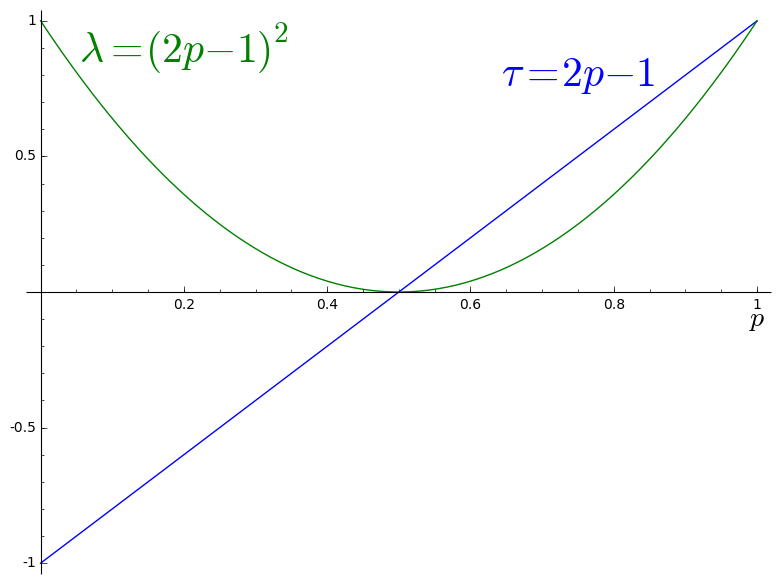
\includegraphics[scale=0.5]{figures/BC_Potenzial2.png}
\end{center}
\caption{Zusammenhang zwischen Wahrscheinlichkeit $p$,
   I/O-Korrela\-tion\index{I/O-Korrelation} $\tau$ und
   Potenzial\index{Potenzial} $\lambda$}\label{fig-bool-pot}
\end{figure}

\begin{sagecode}
\begin{verbatim}

sage: plot1 = plot(2*x-1, (x,0,1))
sage: plot2 = plot((2*x - 1)**2, (x,0,1), color = 'green')
sage: xlabel = text('$p$', (1.0, -0.1), fontsize = 20, color = 'black')
sage: legend1 = text('$\tau = 2p - 1$', (0.75,0.8), fontsize = 30)
sage: legend2 = text('$\lambda = (2p - 1)^2$', (0.2,0.9), fontsize = 30,\\
        color = 'green')
sage: show(plot1 + plot2 + xlabel + legend1 + legend2)
\end{verbatim}
\caption{Plot von I/O-Korrelation\index{I/O-Korrelation} und
   Potenzial\index{Potenzial}}\label{Sage-code-bool-pot}
\end{sagecode}

Der Schlüssel $k$ ist allerdings das Ziel des Angriffs und die
Wahrscheinlichkeit $p_{F,\alpha,\beta,\kappa}(k)$ in der
Angriffssituation unbekannt. Für die Kryptoanalyse ist es daher
angebracht, die Wahrscheinlichkeit einer linearen Relation noch
über alle Schlüssel zu mitteln:
\begin{equation}\label{eq-bool-avrg}
   p_{F,\alpha,\beta,\kappa} := \frac{1}{2^{n+l}}
      \#\{(a,k) \in \F_2^n \times \F_2^l \:|\:
           \kappa(k) = \alpha(a) + \beta(F(a,k)) \}.
\end{equation}
Diese Größe ist, zumindest theoretisch, wenn man die Effizienzfrage
außer Acht lässt, allein aus der Definition der Chiffre $F$ bestimmbar.
Ihre Bestimmung läuft allerdings auf eine Exhaustion aller Klartexte
und Schlüssel hinaus und ist daher bei einer realen Chiffre mit
genügend großen Blocklängen oft wirklich nur theoretisch.
Auch hierfür werden  I/O-Korrelation\index{I/O-Korrelation} und
Potenzial\index{Potenzial} definiert:
\[
   \tau_{F,\alpha,\beta,\kappa} := 2 p_{F,\alpha,\beta,\kappa} - 1,
\]
\[
   \lambda_{F,\alpha,\beta,\kappa} := \tau_{F,\alpha,\beta,\kappa}^2.
\]

Shamir\index{Shamir, Adi}\footnote{%
  Adi Shamir, israelischer Kryptologe, Miterfinder des RSA-Verfahrens,
  $~^{\ast}$6.7.1952.
}
bemerkte schon 1985, dass es überzufällige lineare
Relationen\index{lineare Relation}\index{Relation!linear}
für die S-Boxen des DES\index{DES}-Verfahrens gibt. Es dauerte allerdings weitere
sieben Jahre, bis es Matsui\index{Matsui, Mitsuru}\footnote{%
  Mitsuru Matsui, japanischer Kryptologe, $~^{\ast}$16.9.1961.
}
(nach ersten Versuchen von Gilbert und Chassé 1990 mit der Chiffre FEAL)
gelang, diese Beobachtung systematisch
auszunutzen. Er ging zur Schätzung\index{Maximum-Likelihood-Schätzung}\footnote{%
   Das ist eine sogenannte Maximum-Likelihood-Schätzung, d.\,h.,
   man entscheidet sich für diejenige von mehreren Hypothesen (hier
   sind es nur zwei), unter deren Annahme das Beobachtungsergebnis
   die höchste Wahrscheinlichkeit hat.
} von $\kappa(k)$ wie folgt vor
(im Fall $p_{F,\alpha,\beta,\kappa} > \frac{1}{2}$, sonst muss man
bei der Entscheidung die Werte $0$ und $1$ vertauschen\footnote{%
  Im Fall $p_{F,\alpha,\beta,\kappa} = \frac{1}{2}$ ist die
  Methode in dieser Form unbrauchbar.
}):
\begin{enumerate}
	\item {\bf [Sammelphase]} Man sammelt $N$ Klartext-Geheimtextpaare
	  $(a_1,c_1), \ldots, (a_N,c_N)$.

	\item {\bf [Auszählung]} Man bestimmt die Anzahl
\[
    t := \# \{i = 1, \ldots, N \:|\: \alpha(a_i) + \beta(c_i) = 0\}.
\]

	\item {\bf [Mehrheitsentscheidung]} aufgrund von $t$:
	  \begin{itemize}
	    \item Ist $t > \frac{N}{2}$, schätzt man $\kappa(k) = 0$.
	    \item Ist $t < \frac{N}{2}$, schätzt man $\kappa(k) = 1$.
	  \end{itemize}
\end{enumerate}
Der Fall $t = \frac{N}{2}$ ist unergiebig, kommt aber selten vor -- man
entscheidet zufällig zwischen $0$ und $1$ oder gibt eine entsprechende
Rückmeldung\footnote{%
   am besten beides wie im SageMath-Beispiel~\ref{Sage-code-bool-mats}
}. Im SageMath-Beispiel~\ref{Sage-code-bool-mats}
steht der Programmcode, eine konkrete Anwendung folgt gleich als Beispiel
im nächsten Unterabschnitt.

\begin{sagecode}
\begin{verbatim}

def Matsui_Test(a, b, pc, compl = False):
  """Matsui's test for linear cryptanalysis"""
  N = len(pc)
  results = []
  for pair in pc:
    ax = binScPr(a,pair[0])
    by = binScPr(b,pair[1])
    result = (ax + by) % 2
    results.append(result)
  t = 0
  for bb in results:
    if bb == 0:
      t = t + 1
  if 2*t > N:
    if compl:
      return [t,1,True]
    else:
      return [t,0,True]
  elif 2*t_0 < N:
    if compl:
      return [t,0,True]
    else:
      return [t,1,True]
  else:
    return [t,randint(0,1),False]
\end{verbatim}
\caption{Matsui-Test\index{Matsui-Test}. Die Linearformen sind {\tt a} für $\alpha$ und
   {\tt b} für $\beta$. Die Liste {\tt pc} enthält {\tt N} Paare von Klartext
   und Geheimtext. Der Boolesche Wert {\tt compl} gibt an, ob das
   als Ergebnis geschätzte Bit invertiert werden soll. Die Ausgabe
   ist ein Tripel aus der Anzahl {\tt t} der gezählten Nullen,
   dem geschätzten Bit und einem Booleschen Wert, der angibt, ob das
   Bit deterministisch bestimmt ({\tt True}) oder im Grenzfall
   zufällig bestimmt ({\tt False}) wurde. Verwendet wird die Funktion
   {\tt binScPr} aus dem SageMath-Beispiel~\ref{Sage-code-bool-div-bbl}
   im Anhang~\ref{ss-bool-conv}.}\label{Sage-code-bool-mats}
\end{sagecode}

Wenn man eine lineare Relation\index{lineare Relation}\index{Relation!linear}
mit hinreichend großem Potenzial\index{Potenzial}, d.\,h.
hinreichend weit von $\frac{1}{2}$ abweichender Wahrscheinlichkeit, erwischt hat,
wird die Erfolgswahrscheinlichkeit dieses Verfahrens bei hinreichend
großem $N$ gut sein. Das erlaubt dann, die Anzahl der unbekannten
Schlüsselbits durch Elimination\index{Elimination} um 1 zu verringern.

Als theoretisches Ergebnis aus diesen Überlegungen
werden wir einen Zusammenhang zwischen der Anzahl $N$ von
benötigten Klartextblöcken und der Erfolgswahrscheinlichkeit erhalten,
siehe Tabelle~\ref{tab-bool-N}.

Je mehr solcher linearen Relationen die Angreiferin mit genügend hoher
Gewissheit findet, desto stärker kann sie die Größe des Schlüsselraums
einschränken, bis schließlich eine Exhaustion\index{Exhaustion} über die noch in Frage
kommenden Schlüssel in den Bereich des Machbaren rückt. Ein konkretes
Beispiel in Abschnitt~\ref{ss-bool-mini} wird dies illustrieren.

\subsubsection*{Beispiel}

Für ein konkretes Beispiel mit $n = l = 4$ betrachten wir die
Boolesche Abbildung\footnote{%
   $f$ ist nebenbei bemerkt die S-Box\index{S-Box} $\mathrm{S}_0$
   von {\sc Lucifer}\index{Lucifer},
   das um 1970 als Vorgänger-Verfahren von DES\index{DES} entwickelt wurde.
} $f$, die durch die Wertetabelle~\ref{tab-bool-A1}
gegeben ist, und bilden damit die Bitblock-Chiffre
(s.\,a. Abbildung~\ref{fig-bool-bsp0})
\[
    F\!: \F_2^4 \times \F_2^4 \longrightarrow \F_2^4, \quad
    F(a,k) := f(a + k).
\]
Das SageMath-Beispiel~\ref{Sage-code-Luc-S0} definiert diese Boolesche
Abbildung $f$ unter dem Namen {\tt S0}
und verwendet die Klassen {\tt BoolF} und {\tt BoolMap} aus dem
Anhang~\ref{ss-bool-class}. Dabei geben die Spalten der (impliziten)
definierenden Matrix genau die Werte der Abbildung an, wie man sie auch
in Tabelle~\ref{tab-bool-A1} in der Spalte $y = f(x)$ wiederfindet.
(D.\,h., das SageMath-Beispiel~\ref{Sage-code-Luc-S0} und die
Tabelle~\ref{tab-bool-A1} enthalten äquivalente Definitionen der
Abbildung $f$.)
Eine exemplarische Evaluation illustriert das (für die dritte Spalte,
entsprechend dem Argument {\tt 0010}).

\begin{sagecode}
\begin{verbatim}

f1 = BoolF([1,1,0,1,1,1,1,0,0,0,0,0,1,0,0,1])
f2 = BoolF([1,1,1,0,1,1,0,0,0,1,0,0,0,1,1,0])
f3 = BoolF([0,1,1,1,1,0,1,0,1,1,1,0,0,0,0,0])
f4 = BoolF([0,1,1,0,0,1,1,0,0,0,1,1,1,0,1,0])
S0 = BoolMap([f1,f2,f3,f4])
# Sample evaluation
sage: S0.valueAt([0,0,1,0])
[0, 1, 1, 1]
\end{verbatim}
\caption{Eine Boolesche Abbildung (S-Box $\mathrm{S}_0$ von
   {\sc Lucifer})}\label{Sage-code-Luc-S0}
\end{sagecode}

Wir verschlüsseln mit dem Schlüssel $k =$ \verb:1000:, den wir später zur
Probe angreifen wollen. Für eine lineare Relation betrachten wir die
Linearformen
\[
     \alpha(a) = a_4, \quad \beta(c) = c_1 + c_2 + c_4, \quad \kappa(k) = k_4;
\]
wir werden in Abschnitt~\ref{ss-bool-bsp1} sehen, dass mit diesen
Linearformen die Relation
$\kappa(k) = \alpha(a) + \beta(c)$ für $F$ eine Wahrscheinlichkeit
deutlich $> \frac{1}{2}$ hat. Tabelle~\ref{tab-bool-mats} zeigt die
Verschlüsselung dreier Klartexte $a$, die wir später als bekannte
Klartexte annehmen wollen. Die Werte für $c$ wurden aus der
Wertetabelle~\ref{tab-bool-A1} abgelesen. Die Anzahl $t$ der
beobachteten Werte $0$ von $\alpha(a)$ + $\beta(c)$ ist $t = 2$.
Die Mehrheitsentscheidung führt also zu der Schätzung $k_4 = 0$
(von der wir wissen, dass sie korrekt ist).

\begin{table}
\begin{center}
\begin{tabular}{|c|c|c|c|} \hline
       $x$   & $y=f(x)$& $\alpha(x) = x_4$ & $\beta(y) = y_1+y_2+y_4$ \\ \hline
     0 0 0 0 & 1 1 0 0 &   0   &  0  \\
     0 0 0 1 & 1 1 1 1 &   1   &  1  \\
     0 0 1 0 & 0 1 1 1 &   0   &  0  \\
     0 0 1 1 & 1 0 1 0 &   1   &  1  \\
     0 1 0 0 & 1 1 1 0 &   0   &  0  \\
     0 1 0 1 & 1 1 0 1 &   1   &  1  \\
     0 1 1 0 & 1 0 1 1 &   0   &  0  \\
     0 1 1 1 & 0 0 0 0 &   1   &  0  \\
     1 0 0 0 & 0 0 1 0 &   0   &  0  \\
     1 0 0 1 & 0 1 1 0 &   1   &  1  \\
     1 0 1 0 & 0 0 1 1 &   0   &  1  \\
     1 0 1 1 & 0 0 0 1 &   1   &  1  \\
     1 1 0 0 & 1 0 0 1 &   0   &  0  \\
     1 1 0 1 & 0 1 0 0 &   1   &  1  \\
     1 1 1 0 & 0 1 0 1 &   0   &  0  \\
     1 1 1 1 & 1 0 0 0 &   1   &  1  \\ \hline
\end{tabular}
\end{center}
\caption{Wertetabelle einer Booleschen Abbildung
  $f\!: \F_2^4 \longrightarrow \F_2^4$ und zwei Linearformen}\label{tab-bool-A1}
\end{table}

\begin{table}
\begin{center}
\begin{tabular}{|c|c|c||ccc|}\hline
   $a$  & $a+k$ & $c$  & $\alpha(a)$ & $\beta(c)$ & $\alpha(a)$ + $\beta(c)$ \\
   \hline
   0010 & 1010  & 0011 &     0       &      1     &             1            \\
   0101 & 1101  & 0100 &     1       &      1     &             0            \\
   1010 & 0010  & 0111 &     0       &      0     &             0            \\
   \hline
\end{tabular}
\end{center}
\caption{Schätzung eines Schlüsselbits nach Matsui unter Verwendung von drei
   bekannten Klartexten}\label{tab-bool-mats}
\end{table}

Das war mit dem Bleistift auf Papier ganz leicht auszuzählen. Dennoch
ist der Nachvollzug in SageMath im Hinblick auf kompliziertere Beispiele
instruktiv. Das geschieht im SageMath-Beispiel~\ref{Sage-code-Mats-Expl}.
Dabei wird die Funktion {\tt xor}\index{XOR} aus dem
SageMath-Beispiel~\ref{Sage-code-bool-div-bbl} im Anhang~\ref{ss-bool-conv}
sowie die im SageMath-Beispiel~\ref{Sage-code-Luc-S0}
definierte Abbildung {\tt S0} verwendet. Das Ergebnis \mbox{\tt [2, 0, True]}
besagt, dass $2$ Nullen unter den ausgezählten Werten waren, was zur
Mehrheitsentscheidung $0$ führt, die (wegen {\tt True}) nicht durch
zufällige Auslosung bei Gleichstand ermittelt wurde.

\begin{sagecode}
\begin{verbatim}

sage: k = [1,0,0,0]
sage: alpha = [0,0,0,1]
sage: beta = [1,1,0,1]
sage: plist = [[0,0,1,0],[0,1,0,1],[1,0,1,0]]
sage: xlist = []
sage: xclist = []
sage: pclist = []
sage: for i in range(0,len(plist)):
....:     x = xor(plist[i],k)
....:     xlist.append(x)
....:
sage: xlist
[[1, 0, 1, 0], [1, 1, 0, 1], [0, 0, 1, 0]]
sage: for i in range(0,len(plist)):
....:     val = S0.valueAt(xlist[i])
....:     xclist.append([xlist[i],val])
....:     pclist.append([plist[i],val])
....:
sage: Matsui_Test(alpha,beta,pclist,False)
[2, 0, True]
\end{verbatim}
\caption{Ein Beispiel für den Matsui-Test\index{Matsui-Test}}\label{Sage-code-Mats-Expl}
\end{sagecode}

\noindent Damit das Verfahren im allgemeinen Fall Erfolg verspricht, sind
folgende Fragen zu klären:
\begin{enumerate}
	\item Wie findet man lineare
        Relationen\index{lineare Relation}\index{Relation!linear}
        von möglichst auffälliger
        Wahrscheinlichkeit? Insbesondere im Hinblick darauf, dass die
        Auswertung der Formel~(\ref{eq-bool-avrg}) am Effizienzproblem
        scheitert.
     \item Da Bitblock-Chiffren\index{Bitblock-Chiffre} meistens aus
        vielen Runden\index{Runde} zusammengesetzt sind, fragt man weiter:
	\begin{enumerate}
	  \item Wie findet man bei einer iterierten Bitblock-Chiffre
	    brauchbare lineare Relationen für die Rundenfunktion?
	  \item Wie setzt man diese über die Runden hinweg zu linearen Relationen
	    für die ganze Chiffre zusammen?
	  \item Wie bestimmt man die Wahrscheinlichkeit einer zusammengesetzten
	    linearen Relation für die ganze Chiffre aus der für die einzelnen
	    Runden?
	\end{enumerate}
\end{enumerate}

\noindent Die Antwort auf die erste Frage und Teil (a) der zweiten heißt:
Aus dem linearen Profil\index{lineares Profil}\index{Profil!linear},
siehe Abschnitt~\ref{ss-bool-lpr}. Die anschließenden
Teilfragen führen zur Untersuchung von linearen
Pfaden\index{linearer Pfad}\index{Pfad!linear},
siehe Abschnitt~\ref{ss-bool-path}, und zur Kumulation von
Wahrscheinlichkeiten, siehe Satz~\ref{thm-bool-rrnd}. Für (c) kommt
dabei letztendlich eine brauchbare Faustregel heraus.

\subsection{Beispiel A: Eine Einrunden-Chiffre}\label{ss-bool-bsp1}

Es werden Beispiele betrachtet, die als ernsthafte Blockchiffren viel
zu einfach sind, aber das Prinzip der linearen
Kryptoanalyse\index{lineare Kryptoanalyse}\index{Kryptoanalyse!linear}
anschaulich und nachvollziehbar demonstrieren. Dabei werden stets
Rundenfunktionen der Gestalt $f(a+k)$ betrachtet, d.\,h., der Schlüssel
bzw. ein $n$-bittiger Teil davon wird vor der Anwendung einer bijektiven
S-Box $f\!: \F_2^n \longrightarrow \F_2^n$ binär auf den Klartext
aufaddiert\footnote{%
   Das ist zwar eine sehr spezielle Art, den Schlüssel in das Verfahren
   einzubringen, aber dennoch realistisch. Die paradigmatischen
   Beispiel-Chiffren {\sc Lucifer}\index{Lucifer}, DES\index{DES}
   und AES\index{AES} verfahren so.
   Bei AES \cite{DaRi2002} heißt das \glqq key-alternating cipher structure\grqq.
}. Das einfachste denkbare Modell, die Verschlüsselung nach der
Vorschrift
\[
   c = f(a+k)
\]
wie im Beispiel des Abschnitts~\ref{ss-bool-lka},
siehe Abbildung~\ref{fig-bool-bsp0}\footnote{%
  In den grafischen Darstellungen hier und später wird die Abbildung
  $f$ auf der elementweisen Ebene durch die S-Box S repräsentiert.
},
ist dabei witzlos, da bei bekanntem\index{bekannter Klartext}\index{Klartext!bekannt}
Klartext die Gleichung nach dem
Schlüssel $k$ auflösbar ist\footnote{%
  Die Umkehrabbildung $f^{-1}$ wird hier als der Angreiferin
  bekannt angenommen. Sie ist ja Teil des Algorithmus zur Entschlüsselung.
  Einweg-Verschlüsselungen\index{Einweg-Verschlüsselung},
  bei denen $f^{-1}$ aus $f$ nicht effizient
  herleitbar ist, bilden ein anderes Kapitel der Kryptographie.
}:
\[
   k = f^{-1}(c) + a.
\]

\begin{figure}
\begin{center}
\begin{picture}(268,68)(0,0)
% Mengen
   \put(11,14){$\F_2^n$}
   \put(28,17){\vector(1,0){34}}
   \put(66,14){$\F_2^n$}
   \put(54,26){$\bigoplus$}
   \put(66,54){$\F_2^n$}
   \put(71,51){\vector(0,-1){28}}
   \put(83,17){\vector(1,0){34}}
   \put(94,20){$f$}
   \put(123,14){$\F_2^n$}

% Elemente
   \put(154,14){$a$}
   \put(165,17){\vector(1,0){28}}
   \put(165,14){\line(0,1){6}}
   \put(197,14){$b$}
   \put(197,54){$k$}
   \put(199,51){\vector(0,-1){28}}
   \put(197,51){\line(1,0){6}}
   \put(205,17){\vector(1,0){40}}
   \put(205,14){\line(0,1){6}}
   \put(214,14){\fcolorbox{black}{yellow}{S}}
   \put(251,14){$c$}

% Rahmen
   \put(0,0){\line(1,0){268}}
   \put(0,68){\line(1,0){268}}
   \put(0,0){\line(0,1){68}}
   \put(268,0){\line(0,1){68}}
\end{picture}
\end{center}
\caption{Ein (viel) zu einfaches Beispiel}\label{fig-bool-bsp0}
\end{figure}

\begin{figure}
\begin{center}
\begin{picture}(208,137)(0,0)
% Mengen
   \put(11,83){$\F_2^n$}
   \put(28,85){\vector(1,0){34}}
   \put(66,83){$\F_2^n$}
   \put(54,94){$\bigoplus$}
   \put(66,124){$\F_2^n$}
   \put(71,120){\vector(0,-1){28}}
   \put(83,85){\vector(1,0){34}}
   \put(94,88){$f$}
   \put(125,83){$\F_2^n$}
   \put(140,85){\vector(1,0){34}}
   \put(179,124){$\F_2^n$}
   \put(185,120){\vector(0,-1){28}}
   \put(168,94){$\bigoplus$}
   \put(179,83){$\F_2^n$}

% Elemente
   \put(23,14){$a$}
   \put(34,17){\vector(1,0){28}}
   \put(34,14){\line(0,1){6}}
   \put(71,14){$b$}
   \put(68,54){$k^{(0)}$}
   \put(74,51){\vector(0,-1){28}}
   \put(71,51){\line(1,0){6}}
   \put(80,17){\vector(1,0){40}}
   \put(80,14){\line(0,1){6}}
   \put(91,14){\fcolorbox{black}{yellow}{S}}
   \put(128,14){$b'$}
   \put(179,54){$k^{(1)}$}
   \put(185,51){\vector(0,-1){28}}
   \put(182,51){\line(1,0){6}}
   \put(142,17){\vector(1,0){28}}
   \put(142,14){\line(0,1){6}}
   \put(182,14){$c$}

% Rahmen
   \put(0,0){\line(1,0){208}}
   \put(0,137){\line(1,0){208}}
   \put(0,0){\line(0,1){137}}
   \put(208,0){\line(0,1){137}}
\end{picture}
\end{center}
\caption{Beispiel A: Eine Einrunden-Chiffre}\label{fig-bool-bspA}
\end{figure}

\begin{figure}
\begin{center}
\begin{picture}(85,68)(0,0)
   \put(6,48){$\F_2^n$}
   \put(23,51){\vector(1,0){40}}
   \put(40,54){$f$}
   \put(68,48){$\F_2^n$}
   \put(40,9){$\F_2$}
   \put(17,43){\vector(1,-1){23}}
   \put(17,26){$\alpha$}
   \put(68,43){\vector(-1,-1){23}}
   \put(60,26){$\beta$}
   \put(38,31){$\stackrel{p}{\approx}$}

% Rahmen
   \put(0,0){\line(1,0){85}}
   \put(0,68){\line(1,0){85}}
   \put(0,0){\line(0,1){68}}
   \put(85,0){\line(0,1){68}}
\end{picture}
\end{center}
\caption{Diagramm für eine "`approximative"' lineare
   Relation\index{lineare Relation}\index{Relation!linear}}\label{fig-bool-appr}
\end{figure}

Dieser einfache Angriff wird bei dem etwas komplizierteren Beispiel A mit
\[
   c = f(a+k^{(0)}) + k^{(1)}
\]
verhindert (siehe Abbildung~\ref{fig-bool-bspA}); hier ist der Ansatz der linearen
Kryptoanalyse\index{lineare Kryptoanalyse}\index{Kryptoanalyse!linear}
bereits sinnvoll: Sei $(\alpha,\beta)$ ein Paar von Linearformen\index{Linearform}
mit
\begin{equation}\label{eq-bool-prob}
     \beta\circ f(x) \stackrel{p}{\approx} \alpha(x),
\end{equation}
wobei das Symbol $\stackrel{p}{\approx}$ zu lesen ist als
"`gleich mit Wahrscheinlichkeit $p$"', also
\[
     p = p_{f,\alpha,\beta} :=
     \frac{1}{2^{n}} \cdot \#\{x \in \F_2^n \:|\: \beta\circ f(x) = \alpha(x) \}.
\]
Repräsentiert wird die Formel~(\ref{eq-bool-prob}) durch das Diagramm in
Abbildung~\ref{fig-bool-appr}. Die Linearform $\kappa$ der
allgemeinen Theorie tritt hier nicht explizit auf: Da die
Schlüsselbits auf Klartext und ("`intermediären"') Geheimtext einfach
aufaddiert werden, ist $\kappa = \alpha$ für $k^{(0)}$ und $\kappa = \beta$
für $k^{(1)}$, also $\kappa(k^{(0)}, k^{(1)}) = \alpha(k^{(0)}) + \beta(k^{(1)})$.

Wie hängt das mit der allgemeinen Situation aus Abschnitt~\ref{ss-bool-lka}
zusammen? Für das Beispiel~A ist
\begin{itemize}
   \item die Schlüssellänge $l = 2n$, der Schlüsselraum ist $\F_2^{2n}$, und
      Schlüssel haben die Gestalt $k = (k^{(0)},k^{(1)})$ mit $k^{(0)}, k^{(1)} \in \F_2^n$.
   \item Die Chiffre ist durch die Abbildung
\[
     F\!: \F_2^n \times \F_2^n \times \F_2^n \longrightarrow \F_2^n,
     \quad (a, k^{(0)}, k^{(1)}) \mapsto f(a + k^{(0)}) + k^{(1)},
\]
      definiert.
   \item Die Linearform $\kappa\!: \F_2^n \times \F_2^n \longrightarrow \F_2$
      ist durch $\kappa(k^{(0)},k^{(1)}) = \alpha(k^{(0)}) + \beta(k^{(1)})$ gegeben.
\end{itemize}
Die Wahrscheinlichkeit einer linearen Relation für einen festen
Schlüssel \mbox{$k = (k^{(0)},k^{(1)})$} ist damit
\begin{eqnarray*}
    p_{F,\alpha,\beta,\kappa}(k) & = & \frac{1}{2^n} \cdot
      \#\{a \in \F_2^n \:|\: \kappa(k) = \alpha(a) + \beta(F(a,k)) \} \\
     & = & \frac{1}{2^n} \cdot
      \#\{a \in \F_2^n \:|\: \alpha(k^{(0)}) + \beta(k^{(1)}) = \alpha(a) + \beta(f(a + k^{(0)}) + k^{(1)}) \} \\
     & = & \frac{1}{2^n} \cdot
      \#\{a \in \F_2^n \:|\: \alpha(k^{(0)}) = \alpha(a) + \beta(f(a + k^{(0)})) \},
\end{eqnarray*}
da $\beta(k^{(1)})$ auf beiden Seiten der Gleichung innerhalb der Mengenklammern
vorkommt und daher einfach weggelassen werden kann.

Dieser Ausdruck ist unabhängig von $k^{(1)}$, und an der leicht umgeformten
Gleichung
\[
     p_{F,\alpha,\beta,\kappa}(k) = \frac{1}{2^n} \cdot
      \#\{a \in \F_2^n \:|\: \alpha(a + k^{(0)}) = \beta(f(a + k^{(0)})) \}
\]
sieht man, dass er für alle $k^{(0)}$ den gleichen Wert hat, da bei festem
$k^{(0)}$ mit $a$ auch $a + k^{(0)}$ ganz $\F_2^n$ durchläuft. Dieser Wert
muss daher mit dem Mittelwert über alle $k$ übereinstimmen:
\[
     p_{F,\alpha,\beta,\kappa}(k) = p_{F,\alpha,\beta,\kappa} = \frac{1}{2^n} \cdot
      \#\{x \in \F_2^n \:|\: \alpha(x) = \beta(f(x)) \} = p.
\]
Mit dieser Überlegung ist gezeigt:

\begin{satz}
    In der Situation des Beispiels~A nimmt die Wahrscheinlichkeit $p_{F,\alpha,\beta,\kappa}(k)$
    für jeden Schlüssel $k \in \F_2^{2n}$ den gleichen Wert
\[
     p = \frac{1}{2^n} \cdot \#\{x \in \F_2^n \:|\: \alpha(x) = \beta(f(x)) \}
\]
   an, insbesondere ist $p$ auch der Mittelwert nach Gleichung~(\ref{eq-bool-avrg}).
\end{satz}

Mit den Bezeichnungen aus Abbildung~\ref{fig-bool-bspA} gilt nun
\begin{align*}
   \beta(c) & = \beta(b' + k^{(1)}) = \beta(b') + \beta(k^{(1)}) \\
            & \stackrel{p}{\approx} \alpha(b) + \beta(k^{(1)})
                   = \alpha(a + k^{(0)}) + \beta(k^{(1)})
                        = \alpha(a) + \alpha(k^{(0)}) + \beta(k^{(1)}).
\end{align*}
Als lineare Relation\index{lineare Relation}\index{Relation!linear}
für die Bits des Schlüssels $k = (k^{(0)},k^{(1)})$ erhalten wir
\[
   \alpha(k^{(0)}) + \beta(k^{(1)}) \stackrel{p}{\approx} \alpha(a) + \beta(c).
\]
Ein analoger Schluss lässt sich für die komplementäre Relation
\[
   \beta\circ f(x) \stackrel{1-p}{\approx} \alpha(x) + 1
\]
durchführen. Insgesamt ist damit gezeigt:

\begin{satz}
  Im Beispiel~A sei $(\alpha,\beta)$ ein Paar von Linearformen\index{Linearform} für $f$
  mit der Wahrscheinlichkeit $p$ wie in Formel~(\ref{eq-bool-prob}).
  Dann ist $\hat{p} =$ \mbox{$\max\{p, 1-p\}$} die Erfolgswahrscheinlichkeit für
  die Bestimmung eines Schlüsselbits aus {\em einem} bekannten
  Klartext\index{bekannter Klartext}\index{Klartext!bekannt}
  durch diese lineare Relation\index{lineare Relation}\index{Relation!linear}.
\end{satz}

\subsubsection*{Beispiel}

Nehmen wir als konkretes Beispiel $n = 4$ und für $f$ wieder die S-Box
$\mathrm{S}_0$ von {\sc Lucifer}\index{Lucifer}. Die beiden rechten Spalten der
Tabelle~\ref{tab-bool-A1} zeigen, dass die durch $(\alpha,\beta)$ mit $\alpha(x) = x_4$
und $\beta(y) = y_1+y_2+y_4$ definierte lineare Relation die Wahrscheinlichkeit
$p_{f,\alpha,\beta} = \frac{14}{16} = \frac{7}{8}$ hat\footnote{%
  Deren Größe ist ein starkes Indiz dafür, dass die Designer von
  {\sc Lucifer}\index{Lucifer} die lineare
  Kryptoanalyse\index{lineare Kryptoanalyse}\index{Kryptoanalyse!linear}
  noch nicht kannten.
}.

Die konkreten Rundenschlüssel\index{Rundenschlüssel} seien
$k^{(0)} =$ \verb:1000: und $k^{(1)} =$ \verb:0001:.
Die Tabelle~\ref{tab-bool-linrel} über alle $16$ möglichen
Klartexte zeigt, dass $\alpha(a)+\beta(c)$ den Wert $1 =\alpha(k^{(0)}) + \beta(k^{(1)})$
für die Summe der Schlüsselbits genau $14$-mal annimmt, wie es sein soll.

\begin{table}
\begin{center}
\begin{tabular}{|cccc|c|} \hline
  $a$  & $b$  & $b'$ & $c$  & $\alpha(a)+\beta(c) = a_4 + c_1 + c_2 + c_4$ \\ \hline
  0000 & 1000 & 0010 & 0011 & 1 \\
  0001 & 1001 & 0110 & 0111 & 1 \\
  0010 & 1010 & 0011 & 0010 & 0 \\
  0011 & 1011 & 0001 & 0000 & 1 \\
  0100 & 1100 & 1001 & 1000 & 1 \\
  0101 & 1101 & 0100 & 0101 & 1 \\
  0110 & 1110 & 0101 & 0100 & 1 \\
  0111 & 1111 & 1000 & 1001 & 1 \\
  1000 & 0000 & 1100 & 1101 & 1 \\
  1001 & 0001 & 1111 & 1110 & 1 \\
  1010 & 0010 & 0111 & 0110 & 1 \\
  1011 & 0011 & 1010 & 1011 & 1 \\
  1100 & 0100 & 1110 & 1111 & 1 \\
  1101 & 0101 & 1101 & 1100 & 1 \\
  1110 & 0110 & 1011 & 1010 & 1 \\
  1111 & 0111 & 0000 & 0001 & 0 \\
  \hline
\end{tabular}
\end{center}
\caption{Eine lineare Relation für die Schlüsselbits ($b$ entsteht aus $a$ durch Addition
   von $k^{(0)}$, also ``Umkippen'' des ersten Bits, $b'$ aus $b$ durch Anwendung
   von $f$, $c$ aus $b'$ durch Addition von $k^{(1)}$.}\label{tab-bool-linrel}
\end{table}

Wie groß ist nun die Erfolgswahrscheinlichkeit $p_N$ dafür, diesen Wert
richtig zu schätzen, wenn man $N = 1, 2, \ldots$ zufällige bekannte
Klartexte\index{bekannter Klartext}\index{Klartext!bekannt}
aus der Menge der $2^n$ möglichen zur Verfügung hat (zu gegebenen festen
Linearformen $\alpha$ und $\beta$ mit $p = p_{f,\alpha,\beta}$)? Das ist genau
eine konkrete Einkleidung der Fragestellung der hypergeometrischen Verteilung,
und daher gilt
(ohne Beweis und ohne Erklärung der hypergeometrischen
Verteilung\index{hypergeometrische Verteilung}\index{Verteilung!hypergeometrisch}):

\begin{satz}
  Im Beispiel A sei $(\alpha,\beta)$ ein Paar von Linearformen, das
  eine lineare Relation für $f$ mit der Wahrscheinlichkeit $p$ definiert.
  Dann ist die Erfolgswahrscheinlichkeit für die Bestimmung eines
  Schlüsselbits aus $N$ bekannten Klartexten durch diese lineare
  Relation\index{lineare Relation}\index{Relation!linear}
  gerade die kumulierte Wahrscheinlichkeit $p_N = p_N^{(s)}$ der
  hypergeometrischen Verteilung zu den Parametern $2^n$, $s = \hat{p}\cdot 2^n$
  und $N$ mit $\hat{p} = \max\{p, 1-p\}$.
\end{satz}

Verlässt man die exakte Mathematik und geht, wie oft in der angewandten Statistik,
zu asymptotischen Näherungsformeln über, so kann man unter den (sehr vage
formulierten) Voraussetzungen
"`$p$ nicht zu weit von $\frac{1}{2}$ entfernt, $N \ll 2^n$, aber $N$ nicht
zu klein,"' die hypergeometrische Verteilung\index{hypergeometrische
Verteilung}\index{Verteilung!hypergeometrisch} durch die
Normalverteilung\index{Normalverteilung} approximieren und erhält
\begin{equation}\label{equ-bool-N}
  p_N \approx \frac{1}{\sqrt{2\pi}} \cdot
                      \int_{-\infty}^{\sqrt{N\lambda}} e^{-t^2/2}\,dt,
\end{equation}
wobei $\lambda = (2p - 1)^2$ das Potenzial\index{Potenzial} der linearen Relation ist.
Zusammen mit den bekannten Werten für die Normalverteilung\footnote{%
   Man kann statt mit der Approximation durch die Normalverteilung auch direkt
   mit der hypergeometrischen
   Verteilung\index{hypergeometrische Verteilung}\index{Verteilung!hypergeometrisch}
   rechnen. Dann erhält man,
   besonders bei kleinem $N$, einen genaueren Wert, aber keine so
   einfache geschlossene Formel wie (\ref{equ-bool-N}).
} ergibt das die
Tabelle~\ref{tab-bool-N}. D.\,h., um eine Erfolgswahrscheinlichkeit von etwa
$95\%$ zu erreichen, braucht man $N \approx \frac{3}{\lambda}$ bekannte
Klartexte\index{bekannter Klartext}\index{Klartext!bekannt}.
Im obigen konkreten Beispiel war $p = \frac{7}{8}$, also $\lambda = \frac{9}{16}$,
und die Zahl der nötigen bekannten Klartexte für die $95$-prozentige
Erfolgswahrscheinlichkeit ist nach der Formel $N \approx 5$. Wir waren,
siehe Tabelle~\ref{tab-bool-mats}, schon mit $N = 3$ erfolgreich gewesen;
das ist nicht sehr überraschend, denn wie wir jetzt sehen, war
die Erfolgswahrscheinlichkeit dafür immerhin knapp 90\% (hier ist nämlich
$N\lambda = \frac{27}{16} \approx 1,68\ldots$)\footnote{%
   Hier wird man die Voraussetzung "`$N$ nicht zu klein"' der Approximation
   durch die Normalverteilung\index{Normalverteilung} zu Recht anzweifeln müssen.
   In der Tat kann man leicht die exakten Werte für die hypergeometrische
   Verteilung\index{hypergeometrische Verteilung}\index{Verteilung!hypergeometrisch}
   bestimmen:
   Zieht man aus einer Urne mit $16$ Kugeln, von denen $14$ schwarz und
   $2$ weiß sind, zufällig $3$ Kugeln, so werden diese mit Wahrscheinlichkeit
   $\frac{26}{40}$ alle drei schwarz sein, und mit Wahrscheinlichkeit
   $\frac{13}{40}$ zwei davon schwarz und eine weiß, also mit Wahrscheinlichkeit
   $\frac{39}{40} = 97,5\%$ mindestens zwei schwarz. Das ist also deutlich
   mehr als die aus der Approximationsformel~(\ref{equ-bool-N}) bestimmten 90\%.
   Die übrigen Wahrscheinlichkeiten sind $\frac{1}{40}$ für genau eine schwarze
   Kugel und $0$ für drei weiße.
}.

\begin{table}
\begin{center}
  \begin{tabular}{|c|ccccccc|} \hline
		$N\lambda$ & $1$ & $2$ & $3$ & $4$ & \ldots & $8$ & $9$ \\
		$p_N$ & $84,1\%$ & $92,1\%$ & $95,8\%$ & $97,7\%$ & \ldots &
		                      $99,8\%$ & $99,9\%$ \\ \hline
  \end{tabular}
\end{center}
\caption{Zusammenhang zwischen der Anzahl der bekannten
   Klartexte\index{bekannter Klartext}\index{Klartext!bekannt}
   und der Erfolgs\-wahr\-schein\-lich\-keit}\label{tab-bool-N}
\end{table}

\subsection{Approximationstabelle\index{Approximationstabelle},
   Korrelationsmatrix\index{Korrelationsmatrix} und lineares
   Profil\index{lineares Profil}\index{Profil!linear}}\label{ss-bool-lpr}

Die Häufigkeiten, mit denen lineare
Relationen\index{lineare Relation}\index{Relation!linear} für eine Boolesche
Abbildung\index{Boolesche Abbildung}\index{Abbildung!Boolesche}
(oder S-Box\index{S-Box}) $f\!: \F_2^n \longrightarrow \F_2^q$ gelten, werden
in einer $2^n \times 2^q$-Matrix zusammengefasst, die zu
jedem Paar von Linearformen\index{Linearform} $(\alpha,\beta)$
die Anzahl der Argumente $x$ mit $\beta\circ f(x) = \alpha(x)$ angibt und
{\bf Approximationstabelle\index{Approximationstabelle}}
genannt wird\footnote{%
   Vorsicht mit den Literatur-Referenzen: Oft wird von allen Einträgen
   noch der Wert $2^{n-1}$ abgezogen, so z.\,B. bei der SageMath-Funktion
   {\tt linear\_approximation\_matrix()}.
}\label{fn-lin-appr}.
Für die oben verwendete S-Box $\mathrm{S}_0$ von {\sc Lucifer}\index{Lucifer}
ist sie in Tabelle~\ref{tab-bool-s0} wiedergegeben. Der Eintrag $16$ in
der linken oberen Ecke besagt, dass die Relation $0 = 0$ immer, also
in allen $16$ Fällen gilt, und ist gleichzeitig der Hauptnenner, durch
den man alle Einträge teilen muss, um die Wahrscheinlichkeiten zu
erhalten; im allgemeinen Fall würde dort $2^n$ stehen. Die übrigen Einträge
in der ersten Spalte (entsprechend $\beta = 0$) sind $8$, weil jede von Null
verschiedene Linearform\index{Linearform} $\alpha$ den Wert $0$ in genau der
Hälfte aller Fälle, hier also $8$-mal, annimmt\footnote{%
   In der Sprache der Linearen Algebra\index{lineare Algebra}\index{Algebra!lineare}:
   Der Kern einer Linearform\index{Linearform} $\neq 0$
   ist ein $(n-1)$-dimensionaler Unterraum.
}. Für die erste Zeile gilt das analoge
Argument -- vorausgesetzt, $f$ ist bijektiv\footnote{%
   Im allgemeinen Fall, wo $q \neq n$ sein kann, müsste man hier
   "`balanciert\index{balanciert}"' sagen, d.\,h., alle Urbildmengen sind gleich groß.
   Das geht natürlich nur im Fall $q \leq n$ wirklich.
}.

\begin{table}
\begin{center}
\begin{tabular}{|c|cccccccccccccccc|} \hline
     & 0 & 1 & 2 & 3 & 4 & 5 & 6 & 7 & 8 & 9 &10 &11 &12 &13 &14 &15 \\ \hline
   0 &16 & 8 & 8 & 8 & 8 & 8 & 8 & 8 & 8 & 8 & 8 & 8 & 8 & 8 & 8 & 8 \\
   1 & 8 & 6 & 6 & 8 & 8 & 6 & 6 & 8 & 8 & 6 & 6 & 8 & 8 &14 & 6 & 8 \\
   2 & 8 &10 & 8 & 6 & 4 & 6 & 8 & 6 & 6 &12 & 6 & 8 &10 & 8 & 6 & 8 \\
   3 & 8 &12 &10 & 6 &12 & 8 &10 & 6 & 6 & 6 & 8 & 8 &10 &10 & 8 & 8 \\
   4 & 8 & 8 & 4 & 8 & 8 & 8 & 8 & 4 &10 & 6 & 6 & 6 &10 & 6 &10 &10 \\
   5 & 8 &10 &10 &12 & 8 &10 & 6 & 8 &10 & 8 & 4 &10 &10 & 8 & 8 & 6 \\
   6 & 8 &10 & 8 &10 & 8 &10 & 8 &10 & 8 &10 & 8 & 2 & 8 &10 & 8 &10 \\
   7 & 8 & 8 &10 & 6 & 8 & 8 & 2 & 6 & 8 & 8 &10 & 6 & 8 & 8 &10 & 6 \\
   8 & 8 & 8 & 6 &10 & 6 &10 & 8 & 8 & 4 & 8 &10 &10 &10 &10 &12 & 8 \\
   9 & 8 &10 & 8 &10 & 6 & 4 &10 & 8 & 8 & 6 & 8 & 6 & 6 & 8 &10 & 4 \\
  10 & 8 & 6 &10 & 8 & 6 & 8 & 8 &10 & 6 & 4 & 8 & 6 &12 & 6 & 6 & 8 \\
  11 & 8 &12 & 8 & 8 & 6 & 6 & 6 &10 &10 & 6 &10 &10 & 8 & 8 & 8 &12 \\
  12 & 8 & 8 &10 &10 & 6 &10 & 8 & 4 & 6 & 6 & 8 & 8 & 4 & 8 & 6 &10 \\
  13 & 8 & 6 &12 & 6 & 6 & 8 &10 & 8 &10 & 8 & 6 & 8 & 8 &10 &12 & 8 \\
  14 & 8 & 6 &10 &12 &10 & 4 & 8 & 6 & 8 &10 &10 & 8 &10 & 8 & 8 &10 \\
  15 & 8 & 8 & 8 & 8 &10 & 6 & 6 &10 & 4 & 8 & 4 & 8 & 6 & 6 &10 &10 \\ \hline
\end{tabular}
\end{center}
\caption{Approximationstabelle der S-Box $\mathrm{S}_0$ von {\sc Lucifer}\index{Lucifer} --
   Zeilen- und Spaltenindizes sind durch Zahlen repräsentierte Linearformen,
   siehe Abschnitt~\ref{ss-bool-repr}.
   Die Wahrscheinlichkeiten erhält man nach Division durch 16.}\label{tab-bool-s0}
\end{table}

\begin{table}
\begin{center}
\begin{tabular}{|c|cccccccccccccccc|} \hline
     & 0 & 1 & 2 & 3 & 4 & 5 & 6 & 7 & 8 & 9 &10 &11 &12 &13 &14 &15 \\ \hline
   0 & 1 & 0 & 0 & 0 & 0 & 0 & 0 & 0 & 0 & 0 & 0 & 0 & 0 & 0 & 0 & 0 \\
   1 & 0 &$-\frac{1}{4}$&$-\frac{1}{4}$& 0 & 0 &$-\frac{1}{4}$&$-\frac{1}{4}$& 0 & 0 &$-\frac{1}{4}$&$-\frac{1}{4}$& 0 & 0 &$\frac{3}{4}$&$-\frac{1}{4}$& 0 \\
   2 & 0 &$\frac{1}{4}$& 0 & $-\frac{1}{4}$ &$-\frac{1}{2}$& $-\frac{1}{4}$ & 0 & $-\frac{1}{4}$ & $-\frac{1}{4}$ &$\frac{1}{2}$& $-\frac{1}{4}$ & 0 &$\frac{1}{4}$& 0 & $-\frac{1}{4}$ & 0 \\
   3 & 0 &$\frac{1}{2}$&$\frac{1}{4}$& $-\frac{1}{4}$ &$\frac{1}{2}$& 0 &$\frac{1}{4}$& $-\frac{1}{4}$ & $-\frac{1}{4}$ & $-\frac{1}{4}$ & 0 & 0 &$\frac{1}{4}$&$\frac{1}{4}$& 0 & 0 \\
   4 & 0 & 0 &$-\frac{1}{2}$& 0 & 0 & 0 & 0 &$-\frac{1}{2}$&$\frac{1}{4}$& $-\frac{1}{4}$ & $-\frac{1}{4}$ & $-\frac{1}{4}$ &$\frac{1}{4}$& $-\frac{1}{4}$ &$\frac{1}{4}$&$\frac{1}{4}$\\
   5 & 0 &$\frac{1}{4}$&$\frac{1}{4}$&$\frac{1}{2}$& 0 &$\frac{1}{4}$& $-\frac{1}{4}$ & 0 &$\frac{1}{4}$& 0 &$-\frac{1}{2}$&$\frac{1}{4}$&$\frac{1}{4}$& 0 & 0 & $-\frac{1}{4}$ \\
   6 & 0 &$\frac{1}{4}$& 0 &$\frac{1}{4}$& 0 &$\frac{1}{4}$& 0 &$\frac{1}{4}$& 0 &$\frac{1}{4}$& 0 & $-\frac{3}{4}$ & 0 &$\frac{1}{4}$& 0 &$\frac{1}{4}$\\
   7 & 0 & 0 &$\frac{1}{4}$& $-\frac{1}{4}$ & 0 & 0 & $-\frac{3}{4}$ & $-\frac{1}{4}$ & 0 & 0 &$\frac{1}{4}$& $-\frac{1}{4}$ & 0 & 0 &$\frac{1}{4}$& $-\frac{1}{4}$ \\
   8 & 0 & 0 & $-\frac{1}{4}$ &$\frac{1}{4}$& $-\frac{1}{4}$ &$\frac{1}{4}$& 0 & 0 &$-\frac{1}{2}$& 0 &$\frac{1}{4}$&$\frac{1}{4}$&$\frac{1}{4}$&$\frac{1}{4}$&$\frac{1}{2}$& 0 \\
   9 & 0 &$\frac{1}{4}$& 0 &$\frac{1}{4}$& $-\frac{1}{4}$ &$-\frac{1}{2}$&$\frac{1}{4}$& 0 & 0 & $-\frac{1}{4}$ & 0 & $-\frac{1}{4}$ & $-\frac{1}{4}$ & 0 &$\frac{1}{4}$&$-\frac{1}{2}$\\
  10 & 0 & $-\frac{1}{4}$ &$\frac{1}{4}$& 0 & $-\frac{1}{4}$ & 0 & 0 &$\frac{1}{4}$& $-\frac{1}{4}$ &$-\frac{1}{2}$& 0 & $-\frac{1}{4}$ &$\frac{1}{2}$& $-\frac{1}{4}$ & $-\frac{1}{4}$ & 0 \\
  11 & 0 &$\frac{1}{2}$& 0 & 0 & $-\frac{1}{4}$ & $-\frac{1}{4}$ & $-\frac{1}{4}$ &$\frac{1}{4}$&$\frac{1}{4}$& $-\frac{1}{4}$ &$\frac{1}{4}$&$\frac{1}{4}$& 0 & 0 & 0 &$\frac{1}{2}$\\
  12 & 0 & 0 &$\frac{1}{4}$&$\frac{1}{4}$& $-\frac{1}{4}$ &$\frac{1}{4}$& 0 &$-\frac{1}{2}$& $-\frac{1}{4}$ & $-\frac{1}{4}$ & 0 & 0 &$-\frac{1}{2}$& 0 & $-\frac{1}{4}$ &$\frac{1}{4}$\\
  13 & 0 & $-\frac{1}{4}$ &$\frac{1}{2}$& $-\frac{1}{4}$ & $-\frac{1}{4}$ & 0 &$\frac{1}{4}$& 0 &$\frac{1}{4}$& 0 & $-\frac{1}{4}$ & 0 & 0 &$\frac{1}{4}$&$\frac{1}{2}$& 0 \\
  14 & 0 & $-\frac{1}{4}$ &$\frac{1}{4}$&$\frac{1}{2}$&$\frac{1}{4}$&$-\frac{1}{2}$& 0 & $-\frac{1}{4}$ & 0 &$\frac{1}{4}$&$\frac{1}{4}$& 0 &$\frac{1}{4}$& 0 & 0 &$\frac{1}{4}$\\
  15 & 0 & 0 & 0 & 0 &$\frac{1}{4}$& $-\frac{1}{4}$ & $-\frac{1}{4}$ &$\frac{1}{4}$&$-\frac{1}{2}$& 0 &$-\frac{1}{2}$& 0 & $-\frac{1}{4}$ & $-\frac{1}{4}$ &$\frac{1}{4}$&$\frac{1}{4}$\\ \hline
\end{tabular}
\end{center}\caption{Korrelationsmatrix der S-Box $\mathrm{S}_0$ von {\sc Lucifer}\index{Lucifer} --
   Zeilen- und Spaltenindizes sind durch Zahlen repräsentierte Linearformen.}\label{tab-bool-corr}
\end{table}

\begin{table}
\begin{center}
\begin{tabular}{|c|cccccccccccccccc|} \hline
  &0& 1            & 2            & 3            & 4            & 5            & 6            & 7
     & 8            & 9            &10            &11            &12            &13            &14            &15            \\
\hline
 0&1& 0            & 0            & 0            & 0            & 0            & 0            & 0
     & 0            & 0            & 0            & 0            & 0            & 0            & 0            & 0            \\
 1&0&$\frac{1}{16}$&$\frac{1}{16}$& 0            & 0            &$\frac{1}{16}$&$\frac{1}{16}$& 0
     & 0            &$\frac{1}{16}$&$\frac{1}{16}$& 0            & 0            &$\frac{9}{16}$&$\frac{1}{16}$& 0            \\
 2&0&$\frac{1}{16}$& 0            &$\frac{1}{16}$&$\frac{1}{4}$ &$\frac{1}{16}$& 0            &$\frac{1}{16}$&$\frac{1}{16}$
     &$\frac{1}{4}$ &$\frac{1}{16}$& 0            &$\frac{1}{16}$& 0            &$\frac{1}{16}$& 0            \\
 3&0&$\frac{1}{4}$ &$\frac{1}{16}$&$\frac{1}{16}$&$\frac{1}{4}$ & 0            &$\frac{1}{16}$&$\frac{1}{16}$&$\frac{1}{16}$
     &$\frac{1}{16}$& 0            & 0            &$\frac{1}{16}$&$\frac{1}{16}$& 0            & 0            \\
 4&0& 0            &$\frac{1}{4}$ & 0            & 0            & 0            & 0            &$\frac{1}{4}$ &$\frac{1}{16}$
     &$\frac{1}{16}$&$\frac{1}{16}$&$\frac{1}{16}$&$\frac{1}{16}$&$\frac{1}{16}$&$\frac{1}{16}$&$\frac{1}{16}$\\
 5&0&$\frac{1}{16}$&$\frac{1}{16}$&$\frac{1}{4}$ & 0            &$\frac{1}{16}$&$\frac{1}{16}$& 0            &$\frac{1}{16}$
     & 0            &$\frac{1}{4}$ &$\frac{1}{16}$&$\frac{1}{16}$& 0            & 0            &$\frac{1}{16}$\\
 6&0&$\frac{1}{16}$& 0            &$\frac{1}{16}$& 0            &$\frac{1}{16}$& 0            &$\frac{1}{16}$& 0
     &$\frac{1}{16}$& 0            &$\frac{9}{16}$& 0            &$\frac{1}{16}$& 0            &$\frac{1}{16}$\\
 7&0& 0            &$\frac{1}{16}$&$\frac{1}{16}$& 0            & 0            &$\frac{9}{16}$&$\frac{1}{16}$& 0
     & 0            &$\frac{1}{16}$&$\frac{1}{16}$& 0            & 0            &$\frac{1}{16}$&$\frac{1}{16}$\\
 8&0& 0            &$\frac{1}{16}$&$\frac{1}{16}$&$\frac{1}{16}$&$\frac{1}{16}$& 0            & 0            &$\frac{1}{4}$
     & 0            &$\frac{1}{16}$&$\frac{1}{16}$&$\frac{1}{16}$&$\frac{1}{16}$&$\frac{1}{4}$ & 0            \\
 9&0&$\frac{1}{16}$& 0            &$\frac{1}{16}$&$\frac{1}{16}$&$\frac{1}{4}$&$\frac{1}{16}$& 0            & 0
     &$\frac{1}{16}$& 0            &$\frac{1}{16}$&$\frac{1}{16}$& 0            &$\frac{1}{16}$&$\frac{1}{4}$ \\
10&0&$\frac{1}{16}$&$\frac{1}{16}$& 0            &$\frac{1}{16}$& 0            & 0            &$\frac{1}{16}$&$\frac{1}{16}$
     &$\frac{1}{4}$ & 0            &$\frac{1}{16}$&$\frac{1}{4}$ &$\frac{1}{16}$&$\frac{1}{16}$& 0            \\
11&0&$\frac{1}{4}$ & 0            & 0            &$\frac{1}{16}$&$\frac{1}{16}$&$\frac{1}{16}$&$\frac{1}{16}$&$\frac{1}{16}$
     &$\frac{1}{16}$&$\frac{1}{16}$&$\frac{1}{16}$& 0            & 0            & 0            &$\frac{1}{4}$ \\
12&0& 0            &$\frac{1}{16}$&$\frac{1}{16}$&$\frac{1}{16}$&$\frac{1}{16}$& 0            &$\frac{1}{4}$ &$\frac{1}{16}$
     &$\frac{1}{16}$& 0            & 0            &$\frac{1}{4}$ & 0            &$\frac{1}{16}$&$\frac{1}{16}$\\
13&0&$\frac{1}{16}$&$\frac{1}{4}$&$\frac{1}{16}$&$\frac{1}{16}$& 0            &$\frac{1}{16}$& 0            &$\frac{1}{16}$
     & 0            &$\frac{1}{16}$& 0            & 0            &$\frac{1}{16}$&$\frac{1}{4}$ &$0$\\
14&0&$\frac{1}{16}$&$\frac{1}{16}$&$\frac{1}{4}$ &$\frac{1}{16}$&$\frac{1}{4}$ & 0            &$\frac{1}{16}$& 0
     &$\frac{1}{16}$&$\frac{1}{16}$& 0            &$\frac{1}{16}$& 0            & 0            &$\frac{1}{16}$\\
15&0& 0            & 0            & 0            &$\frac{1}{16}$&$\frac{1}{16}$&$\frac{1}{16}$&$\frac{1}{16}$&$\frac{1}{4}$
     & 0            &$\frac{1}{4}$ & 0            &$\frac{1}{16}$&$\frac{1}{16}$&$\frac{1}{16}$&$\frac{1}{16}$\\
\hline
\end{tabular}
\end{center}\caption{Lineares Profil der S-Box $\mathrm{S}_0$ von {\sc Lucifer}\index{Lucifer} --
   Zeilen- und Spaltenindizes sind durch Zahlen repräsentierte Linearformen.}\label{tab-bool-lp0}
\end{table}

Die {\bf Korrelationsmatrix}\index{Korrelationsmatrix} und das
{\bf lineare Profil}\index{lineares Profil}\index{Profil!linear}\footnote{%
   oder auch Linearitätsprofil\index{Linearitätsprofil}; nicht zu verwechseln
   mit dem linearen
   Komplexitätsprofil\index{lineares Komplexitätsprofil}\index{Komplexitätsprofil!linear} einer
   Bitfolge, das mit Hilfe von linearen Schieberegistern
   definiert wird und auch oft Linearitätsprofil genannt wird.
   }
sind die entsprechenden Matrizen, deren Einträge
jeweils die I/O-Korrelation\index{I/O-Korrelation} bzw. das
Potenzial\index{Potenzial} der linearen Relation enthalten.
Man erhält die Korrelationsmatrix\index{Korrelationsmatrix} aus der
Approximationstabelle\index{Approximationstabelle}, indem man erst
die Einträge durch $2^n$ dividiert, um die jeweiligen Wahrscheinlichkeiten $p$
zu erhalten; dann muss man noch die Wahrscheinlichkeiten nach der Formel
$\tau = 2p - 1$ in I/O-Korrelationen\index{I/O-Korrelation} umrechnen.
Das lineare Profil\index{lineares Profil}\index{Profil!linear}
entsteht dann, indem man die Einträge der
Korrelationsmatrix\index{Korrelationsmatrix} einzeln quadriert.

Für $\mathrm{S}_0$ ist die Korrelationsmatrix\index{Korrelationsmatrix}
in Tabelle~\ref{tab-bool-corr} und
das lineare Profil\index{lineares Profil}\index{Profil!linear}
in Tabelle~\ref{tab-bool-lp0} wiedergegeben. Auch hier sind
die erste Zeile und die erste Spalte auffällig; die Nullen besagen, dass
eine lineare Relation\index{lineare Relation}\index{Relation!linear},
an der die Linearform $0$ beteiligt ist, das
Potenzial $0$ hat, also nutzlos ist. Die $1$ links oben in der Ecke
drückt aus, dass die Relation $0 = 0$ immer gilt, ist aber ebenso nutzlos.
Das oben herausgepickte
Paar $(\alpha,\beta)$ mit $\alpha(x) = x_4$ (repräsentiert durch \verb:0001: $\hat{=}\, 1$)
und $\beta(y) = y_1+y_2+y_4$ (repräsentiert durch \verb:1101: $\hat{=}\, 13$) in Zeile 1,
Spalte 13, hat den Maximalwert\footnote{%
  Der eigentliche Maximalwert $1$ in der linken oberen Ecke wird
  ignoriert, da er nutzlos ist.
} $\frac{9}{16}$ für das Potenzial, der aber auch noch
an den Stellen $(6,11)$ und $(7,6)$ des linearen Profils vorkommt.

\subsubsection*{Effiziente Berechnung per Fourier-Transformation}

Man kann die Approximationstabelle "`naiv"' durch Auszählen gewinnen
und daraus die Korrelationsmatrix und das lineare Profil durch
einfache (elementweise) Umrechnung herleiten. Ein effizienterer
Algorithmus verwendet die Fourier\footnote{%
   Joseph Fourier\index{Fourier, Joseph}, französischer Mathematiker und Physiker,
   21.3.1768--16.5.1830
}-Transformation\index{Fourier-Transformation}, die im uns betreffenden
binären Fall besonders einfach ist und wegen historisch unabhängiger
Erfindungen hier auch Hadamard\footnote{%
   Jacques Hadamard\index{Hadamard, Jacques}, französischer Mathematiker, 8.12.1865--17.10.1963
}-Transformation\index{Hadamard-Transformation} oder Walsh\footnote{%
   Joseph L. Walsh\index{Walsh, Joseph L.}, US-amerikanischer Mathematiker, 21.9.1895--6.12.1973
}-Transformation\index{Walsh-Transformation}
genannt wird. Diese Transformation wandelt eine {\em reellwertige} (!)
Funktion $\varphi\!: \F_2^m \longrightarrow \R$ wieder in eine
reellwertige Funktion $\hat{\varphi}\!: \F_2^m \longrightarrow \R$
um, die durch
\[
  \hat{\varphi}(u) := \sum_{x \in \F_2^m} \varphi(x)\cdot (-1)^{u\cdot x}.
\]
definiert ist\footnote{%
   Das ist ein Spezialfall der diskreten
   Fourier-Transformation\index{Fourier-Transformation!diskret}. Im
   allgemeinen Fall würde man statt $-1$ die komplexe $N$-te
   Einheitswurzel\index{Einheitswurzel}
   $\zeta = e^{2\pi i/N}$ verwenden und komplexwertige Funktionen über
   dem Ring $\Z/N\Z$ statt über $\F_2 = \Z/2\Z$ transformieren -- oder
   Funktionen auf $\Z^m$, die in jeder Variablen die Periode $N$ haben.
   Im binären Fall ist $N = 2$, und weil die zweite Einheitswurzel $-1$
   reell ist, reicht es hier, die Diskussion auf reellwertige Funktionen
   zu beschränken.
}. Dabei ist $u\cdot x$ das kanonische Skalarprodukt\index{Skalarprodukt}
in $\F_2^m$. Der Exponent ist also ein Bit, aber das passt schon,
da über der Basis $-1$ für jeden ganzzahligen Exponenten nur die
Restklasse modulo $2$ relevant ist.

Wir betrachten nun eine Boolesche
Abbildung\index{Boolesche Abbildung}\index{Abbildung!Boolesche}
$f\!: \F_2^n \longrightarrow \F_2^q$ und ihre
{\bf Indikatorfunktion}\index{Indikatorfunktion}
$\vartheta_f: \F_2^n \times \F_2^q \longrightarrow \R$,
\[
  \vartheta_f(x,y) := \left\{ \begin{array}{ll}
                     1, & \textrm{wenn } y = f(x), \\
                     0  & \textrm{sonst.}
                   \end{array} \right.
\]
Bestimmen wir die Fourier-Transformation\index{Fourier-Transformation}
davon (mit $m = n+q$, wobei die
Variablen auf Blöcke der Längen $n$ und $q$ verteilt werden):
\begin{eqnarray*}
  \hat{\vartheta}_f(u,v) & = & \sum_{x \in \F_2^n} \sum_{y \in \F_2^q}
                            \vartheta_f(x,y) (-1)^{u\cdot x + v\cdot y} \\
    & = & \sum_{x \in \F_2^n} (-1)^{u\cdot x + v\cdot f(x)}.
\end{eqnarray*}
Im Exponenten stehen die Linearformen\index{Linearform} $x \mapsto u \cdot x$ auf $\F_2^n$,
die wir mit $\alpha$ bezeichnen wollen, und $y \mapsto v \cdot y$ auf $\F_2^q$,
der wir den Namen $\beta$ geben. Dann ist $u$ die Bitblock-Interpretation
von $\alpha$ und $v$ die von $\beta$, und wir sehen im Exponenten etwas Bekanntes,
das uns an die lineare
Kryptoanalyse\index{lineare Kryptoanalyse}\index{Kryptoanalyse!linear} erinnert:
\[
     \alpha(x) + \beta \circ f(x).
\]
Ist $\alpha(x) = \beta \circ f(x)$, so ist der Exponent $0$, der
Summand also $1$. Andernfalls ist der Exponent $1$ und der Summand $-1$.
Es werden also $2^n \cdot p_{f,\alpha,\beta}$ Einsen und
$2^n - 2^n \cdot p_{f,\alpha,\beta}$ "`Minus-Einsen"' aufsummiert, d.\,h.,
die Summe ist
\[
     2^n \cdot [p_{f,\alpha,\beta} - (1 - p_{f,\alpha,\beta})]
     = 2^n \cdot \tau_{f,\alpha,\beta}.
\]
Somit ist $\hat{\vartheta}_f$ bis auf den Normierungsfaktor $2^n$ die
I/O-Korrelation\index{I/O-Korrelation} von $(\alpha, \beta)$.

Die Fourier-Transformierte der Indikatorfunktion\index{Indikatorfunktion}
einer Booleschen Abbildung\index{Boolesche Abbildung}\index{Abbildung!Boolesche}
$f\!\!: \F_2^n \longrightarrow \F_2^q$, also
$\hat{\vartheta_f}\!\!: \F_2^n \times \F_2^q \longrightarrow \R$,
wird oft das (Walsh-) {\bf Spektrum}\index{Spektrum}\index{Walsh-Spektrum}
von $f$ genannt. Wir haben also gezeigt:

\begin{satz}\label{hwtchar}
  Für eine Boolesche Abbildung $f\!:\F_2^n \longrightarrow \F_2^q$
  ist das Spektrum\index{Spektrum} genau das $2^n$-fache der
  Korrelationsmatrix\index{Korrelationsmatrix}.
\end{satz}

Dieser Satz hat große theoretische und praktische Bedeutung:
\begin{itemize}
   \item Auf der theoretischen Seite führt er zu sehr eleganten und
      knappen Beweisen von Aussagen über die
      Korrelationsmatrix\index{Korrelationsmatrix} und
      die mit ihr verwandten Objekte \cite{Pomm2008}.
   \item Auf der praktischen Seite ermöglicht er die Berechnung der
      Korrelationsmatrix (und damit auch der
      Approximationstabelle\index{Approximationstabelle} und
      des lineren Profils\index{lineares Profil}\index{Profil!linear})
      durch die {\em schnelle\index{Fourier-Transformation}
      Fourier-Transformation\index{Fourier-Transformation!schnell}}\footnote{%
         englisch: Fast Fourier Transformation\index{FFT},
         abgekürzt FFT\index{FFT}
      }, die mithilfe binärer Rekursion\index{binäre Rekursion}\index{Rekursion!binär}
      den Aufwand (fast) um einen Faktor $2^n$ drückt.
\end{itemize}
Wie effizient ist das? Der Einfachheit halber beschränken wir uns
auf den wichtigsten Fall $n = q$. Der naive Aufwand erfordert zur
Bestimmung von $p_{f,\alpha,\beta}$ (und damit auch von
$\tau_{f,\alpha,\beta}$) bei festen $\alpha$ und $\beta$ das
Durchzählen von $2^n$ Argumenten, wenn die Abbildung durch
die Wertetabelle gegeben ist. Der gesamte Aufwand dafür ist also
$2^n \cdot 2^n \cdot 2^n$.

Die Erklärung der schnellen Fourier-Transformation würde hier zu
weit führen (siehe dazu \cite{Pomm2008}). Sie steckt in der Funktion
\verb:wtr(): aus dem Anhang~\ref{ss-bool-walsh}. Ohne Beweis
sei vermerkt, dass die schnelle Fourier-Transformation\index{Fourier-Transformation!schnell}
einer reellwertigen Funktion $\F_2^m \longrightarrow \R$ insgesamt
$3m \cdot 2^m$ einfache reelle Operationen erfordert, die man
für Funktionen mit Werten in $\{-1, 1\}$ naiv zählen kann,
denn es kommen nur ganze Zahlen vor, die nicht allzu groß
werden. Das macht hier also $3 \cdot 2n \cdot 2^{2n}$ Operationen.

Eigentlich sollte man den Aufwand eines Algorithmus aber durch die
Größe $N$ des Inputs beschreiben. Dieser besteht hier aus der
Wertetabelle\index{Wertetabelle} einer Booleschen
Abbildung\index{Boolesche Abbildung}\index{Abbildung!Boolesche}
$\F_2^n \longrightarrow \F_2^n$,
also ist $N = n \cdot 2^n$ -- es müssen $n$ Komponentenfunktionen
für je $2^n$ Argumente definiert werden. So gesehen ist der naive
Aufwand (fast) kubisch, der Aufwand des schnellen Algorithmus nur
noch (im wesentlichen) quadratisch.

Für den Kryptographen ist allerdings die Blocklänge der relevante
Parameter. Unter diesem Gesichtspunkt wächst der Aufwand so oder
so mehr oder weniger stark exponenziell. Immerhin ist die
Berechnung für "`kleine"' S-Boxen, mindestens bis zur Blocklänge $8$,
algorithmisch sehr effizient.

Die Berechnung von Korrelationsmatrix\index{Korrelationsmatrix},
Approximationstabelle\index{Approximationstabelle}\footnote{%
  Zur Berechnung der Approximationstabelle kann man auch die Funktion
  {\tt S0.linear\_approximation\_matrix()}
  der SageMath-Klasse {\tt sage.crypto.mq.sbox.SBox} verwenden, wenn man
  zuvor {\tt S0 = mq.SBox(12,15,7,10,14,13,11,0,2,6,3,1,9,4,5,8)}
  definiert. Achtung: siehe Fußnote auf Seite~\pageref{fn-lin-appr}.
} und linearem Profil\index{lineares Profil}\index{Profil!linear}
von $\mathrm{S}_0$ wird im
SageMath-Beispiel~\ref{Sage-code-bool-lpr} wiedergegeben. (Die Einträge der
Ergebnismatrix \verb:Spec: sind durch $16$, die von \verb:linProf:
durch $256$ zu dividieren.)

\begin{sagecode}
\begin{verbatim}

sage: Spec = S0.wspec()
sage: ApprT = S0.linApprTable()
sage: linProf = S0.linProf()
\end{verbatim}
\caption{Korrelationsmatrix\index{Korrelationsmatrix},
   Approximationstabelle\index{Approximationstabelle} und lineares
   Profil\index{lineares Profil}\index{Profil!linear}
   der S-Box $\mathrm{S}_0$}\label{Sage-code-bool-lpr}
\end{sagecode}

Wird die Methode {\tt linProf()} mit dem zusätzlichen Parameter
{\tt extended=True} aufgerufen, siehe SageMath-Beispiel~\ref{Sage-code-bool-lprext},
gibt sie auch den maximalen Eintrag aus,
zusammen mit allen Index-Paaren, bei denen dieser auftritt. In der
Approximationstabelle\index{Approximationstabelle} oder der
Korrelationsmatrix\index{Korrelationsmatrix} kann man dann nachsehen,
ob die entsprechende
Relation eine Wahrscheinlichkeit größer oder kleiner als $\frac{1}{2}$
hat, ob also bei der Schätzung eines Bits nach Matsui das Komplement
zu wählen ist.

\begin{sagecode}
\begin{verbatim}

sage: lProf = S0.linProf(extended=True)
sage: lProf[0]
[...]
sage: print("Maximum entry:", lProf[1], "| with denominator:", lProf[2])
('Maximum entry:', 144, '| with denominator:', 256)
sage: print("at indices:", lProf[3])
('at indices:', [[1, 13], [6, 11], [7, 6]])
sage: Spec = S0.wspec()
sage: for coord in lProf[3]:
....:     if (Spec[coord[0]][coord[1]] < 0):
....:         print ("For relation at", coord, "take complement.")
....:
('For relation at', [6, 11], 'take complement.')
('For relation at', [7, 6], 'take complement.')
\end{verbatim}
\caption{Lineares Profil\index{lineares Profil}\index{Profil!linear}
   der S-Box $\mathrm{S}_0$ mit Auswertung}\label{Sage-code-bool-lprext}
\end{sagecode}

\subsection{Beispiel B: Eine Zweirunden-Chiffre}\label{ss-bool-2rd}

Die Rundenabbildung
\[
   f\!: \F_2^n \times \F_2^q \longrightarrow \F_2^n
\]
einer Bitblock-Chiffre wird jetzt über zwei Runden iteriert mit
Rundenschlüsseln\index{Rundenschlüssel} $k^{(i)} \in \F_2^q$
wie in Abbildung~\ref{fig-bool-2rd} grafisch dargestellt\footnote{%
  Im Grunde genommen war das Beispiel~A schon eine Zweirunden-Chiffre:
  Man könnte in Abbildung~\ref{fig-bool-bspA} am Ende noch eine
  weitere S-Box anfügen; diese wäre kryptologisch irrelevant, da
  sie als nicht-geheimer Teil des Algorithmus der Kryptoanalytikerin
  bekannt wäre und einfach "`abgestreift"' (d.\,h., ihre Inverse
  auf den Geheimtext angewendet) werden könnte. Dem entspricht,
  dass in Beispiel~A ja zwei Teilschlüssel verwendet werden.
  Analog ist das Beispiel~B in diesem Abschnitt auch schon als
  Dreirunden-Chiffre interpretierbar. Wir schließen uns hier
  aber der üblichen Rundenzählung an.
}.

\begin{figure}
\begin{center}
\begin{picture}(350,230)(0,0)
   \put(51,208){$a =$}
   \put(88,205){\framebox(23,17){$c^{(0)}$}}
   \put(100,202){\vector(0,-1){28}}
   \put(97,162){$f$}
   \put(100,165){\circle{17}}
   \put(142,165){\vector(-1,0){31}}
   \put(145,157){\framebox(23,17){$k^{(1)}$}}
   \put(100,154){\vector(0,-1){28}}
   \put(20,108){$f(c^{(0)},k^{(1)}) =$}
   \put(88,105){\framebox(23,17){$c^{(1)}$}}
   \put(100,103){\vector(0,-1){28}}
   \put(97,63){$f$}
   \put(100,66){\circle{17}}
   \put(142,66){\vector(-1,0){31}}
   \put(145,57){\framebox(23,17){$k^{(2)}$}}
   \put(100,57){\vector(0,-1){28}}
   \put(2,12){$c = f(c^{(1)},k^{(2)}) =$}
   \put(88,9){\framebox(23,17){$c^{(2)}$}}
% Formeln
   \put(194,171){\sf Lineare Relation $(\alpha_1,\beta_1,\kappa_1)$}
   \put(194,151){\sf mit $\kappa_1(k^{(1)}) \stackrel{p_1}{\approx}
                                           \alpha_1(c^{(0)}) + \beta_1(c^{(1)})$}
   \put(194,71){\sf Lineare Relation $(\alpha_2,\beta_2,\kappa_2)$}
   \put(194,51){\sf mit $\kappa_2(k^{(2)}) \stackrel{p_2}{\approx}
                                           \alpha_2(c^{(1)}) + \beta_2(c^{(2)})$}
% Rahmen
   \put(0,0){\line(1,0){350}}
   \put(0,230){\line(1,0){350}}
   \put(0,0){\line(0,1){230}}
   \put(350,0){\line(0,1){230}}
\end{picture}
\end{center}
\caption{Allgemeine Zweirunden-Chiffre}\label{fig-bool-2rd}
\end{figure}

Es gelten also die linearen Relationen
\[
   \kappa_1(k^{(1)}) \stackrel{p_1}{\approx} \alpha_1(c^{(0)}) + \beta_1(c^{(1)})
\]
mit Wahrscheinlichkeit $p_1$, I/O-Korrelation $\tau_1 = 2p_1 - 1$ und
Potenzial $\lambda_1 = \tau_1^2$ und
\[
   \kappa_2(k^{(2)}) \stackrel{p_2}{\approx} \alpha_2(c^{(1)}) + \beta_2(c^{(2)})
\]
mit Wahrscheinlichkeit $p_2$, I/O-Korrelation $\tau_2 = 2p_2 - 1$ und
Potenzial $\lambda_2 = \tau_2^2$.
Die beiden linearen Relationen sind {\bf kombinierbar}, wenn $\alpha_2 = \beta_1$.
Dann gilt eine lineare Relation für Schlüsselbits, ausgedrückt durch
den (bekannten) Klartext $c^{(0)} = a$ und den Geheimtext $c^{(2)} = c$:
\[
   \kappa_1(k^{(1)}) + \kappa_2(k^{(2)}) \stackrel{p}{\approx}
      \alpha_1(c^{(0)}) + \beta_2(c^{(2)})
\]
mit einer gewissen Wahrscheinlichkeit $p$, einer I/O-Korrelation\index{I/O-Korrelation}
$\tau$ und einem Potenzial\index{Potenzial} $\lambda$,
die im Allgemeinen von $k = (k^{(1)},k^{(2)})$ abhängen und nicht leicht zu
bestimmen sind. Daher betrachten wir wieder
ein vereinfachtes Beispiel, das Beispiel B aus Abbildung~\ref{fig-bool-bspB}.
Die Verschlüsselung geschieht also sukzessive nach den Formeln
\[
   b^{(0)} = a+k^{(0)},\: a^{(1)} = f_1(b^{(0)}),\: b^{(1)} = a^{(1)}+k^{(1)},\:
   a^{(2)} = f_2(b^{(1)}),\: c = a^{(2)}+k^{(2)}.
\]
(Dabei wird $f_1$ durch die S-Box $\mathrm{S}_0$ und $f_2$ durch die S-Box
$\mathrm{S}_1$ beschrieben, die auch mit $\mathrm{S}_0$ identisch sein
kann\footnote{%
   D.\,h., wir lassen hier zu, dass die Rundenfunktionen der verschiedenen
   Runden unterschiedlich sind. Das hat den Grund, dass in den praktisch
   wichtigen Chiffren die Rundenfunktion aus mehreren parallelen S-Boxen
   besteht und wegen der zwischengeschalteten Permutationen ein Input-Bit
   auf seinem Weg durch die Runden durch verschiedene S-Boxen geleitet
   werden kann, s. Abschnitt~\ref{ss-bool-mini}.
}.) Auch hier verhindert das zusätzliche Aufaddieren
von Schlüsselbits nach der letzten Runde, dass diese, also $f_2$, einfach
"`abgestreift"' werden kann, wie schon bei Beispiel A.

Im Vergleich zur allgemeinen Situation aus Abschnitt~\ref{ss-bool-lka}
gilt im Beispiel~B:
\begin{itemize}
   \item Die Schlüssellänge ist $l = 3n$, der Schlüsselraum ist $\F_2^{3n}$, und
      Schlüssel haben die Gestalt $k = (k^{(0)},k^{(1)},k^{(2)})$ mit
      $k^{(0)}, k^{(1)}, k^{(2)} \in \F_2^n$.
   \item Die Chiffre ist durch die Abbildung
\[
     F\!: \F_2^n \times \F_2^n \times \F_2^n \times \F_2^n \longrightarrow \F_2^n,
     \quad (a, k^{(0)}, k^{(1)}, k^{(2)}) \mapsto f_2(f_1(a + k^{(0)}) + k^{(1)}) + k^{(2)},
\]
      definiert.
   \item Die Linearform $\kappa\!\!: \F_2^n \times \F_2^n \times \F_2^n \longrightarrow \F_2$
      ist durch
      $\kappa(k^{(0)},k^{(1)},k^{(2)}) = \alpha(k^{(0)}) + \beta(k^{(1)}) + \gamma(k^{(2)})$
      gegeben.
\end{itemize}
Dabei ist $(\alpha,\beta)$ eine lineare Relation für $f_1$ mit Wahrscheinlichkeit
$p_1$, I/O-Korrelation $\tau_1$ und Potenzial $\lambda_1$
und $(\beta,\gamma)$ eine für $f_2$ mit
Wahrscheinlichkeit $p_2$, I/O-Korrelation $\tau_2$ und Potenzial $\lambda_2$
(das gleiche $\beta$, d.\,h., die linearen Relationen sind kombinierbar), und
\begin{eqnarray*}
     p_1 & = & \frac{1}{2^n}\cdot \#\{x \in \F_2^n \:|\: \beta \circ f_1(x) = \alpha(x) \} \\
     p_2 & = & \frac{1}{2^n}\cdot \#\{y \in \F_2^n \:|\: \gamma \circ f_2(y) = \beta(y) \}
\end{eqnarray*}

\begin{figure}
\begin{center}
\begin{picture}(320,170)(0,0)
% Mengen
   \put(11,111){$\F_2^n$}
   \put(28,114){\vector(1,0){34}}
   \put(66,111){$\F_2^n$}
   \put(54,123){$\bigoplus$}
   \put(66,151){$\F_2^n$}
   \put(71,148){\vector(0,-1){28}}
   \put(83,114){\vector(1,0){34}}
   \put(94,117){$f_1$}
   \put(123,111){$\F_2^n$}
   \put(140,114){\vector(1,0){34}}
   \put(179,151){$\F_2^n$}
   \put(185,148){\vector(0,-1){28}}
   \put(168,123){$\bigoplus$}
   \put(179,111){$\F_2^n$}
   \put(197,114){\vector(1,0){34}}
   \put(208,117){$f_2$}
   \put(236,111){$\F_2^n$}
   \put(254,114){\vector(1,0){34}}
   \put(293,151){$\F_2^n$}
   \put(299,148){\vector(0,-1){28}}
   \put(282,123){$\bigoplus$}
   \put(293,111){$\F_2^n$}

   \put(97,71){$\F_2$}
   \put(74,105){\vector(1,-1){23}}
   \put(74,88){$\alpha$}
   \put(125,105){\vector(-1,-1){23}}
   \put(117,88){$\beta$}
   \put(94,94){$\stackrel{p_1}{\approx}$}
   \put(211,71){$\F_2$}
   \put(188,105){\vector(1,-1){23}}
   \put(188,88){$\beta$}
   \put(239,105){\vector(-1,-1){23}}
   \put(231,88){$\gamma$}
   \put(208,94){$\stackrel{p_2}{\approx}$}

% Elemente
   \put(23,14){$a$}
   \put(34,17){\vector(1,0){28}}
   \put(34,14){\line(0,1){6}}
   \put(67,14){$b^{(0)}$}
   \put(68,54){$k^{(0)}$}
   \put(74,51){\vector(0,-1){28}}
   \put(71,51){\line(1,0){6}}
   \put(83,17){\vector(1,0){40}}
   \put(83,14){\line(0,1){6}}
   \put(91,14){\fcolorbox{black}{yellow}{$\mathrm{S}_0$}}
   \put(125,14){$a^{(1)}$}
   \put(179,54){$k^{(1)}$}
   \put(185,51){\vector(0,-1){28}}
   \put(182,51){\line(1,0){6}}
   \put(142,17){\vector(1,0){28}}
   \put(142,14){\line(0,1){6}}
   \put(180,14){$b^{(1)}$}

   \put(197,17){\vector(1,0){40}}
   \put(197,14){\line(0,1){6}}
   \put(205,14){\fcolorbox{black}{yellow}{$\mathrm{S}_1$}}
   \put(239,14){$a^{(2)}$}
   \put(293,54){$k^{(2)}$}
   \put(299,51){\vector(0,-1){28}}
   \put(296,51){\line(1,0){6}}
   \put(256,17){\vector(1,0){28}}
   \put(256,14){\line(0,1){6}}
   \put(296,14){$c$}

% Rahmen
   \put(0,0){\line(1,0){320}}
   \put(0,170){\line(1,0){320}}
   \put(0,0){\line(0,1){170}}
   \put(320,0){\line(0,1){170}}
\end{picture}
\end{center}
\caption{Beispiel B: Eine Zweirunden-Chiffre}\label{fig-bool-bspB}
\end{figure}

Dann gilt mit den Bezeichnungen aus Abbildung~\ref{fig-bool-bspB}
\begin{align*}
   \gamma(c) & = \gamma(a^{(2)}) + \gamma(k^{(2)})
                   \stackrel{p_2}{\approx} \beta(b^{(1)}) + \gamma(k^{(2)})
                   = \beta(a^{(1)}) + \beta(k^{(1)}) + \gamma(k^{(2)}) \\
             & \stackrel{p_1}{\approx} \alpha(b^{(0)}) + \beta(k^{(1)}) + \gamma(k^{(2)})
                   = \alpha(a) + \alpha(k^{(0)}) + \beta(k^{(1)}) + \gamma(k^{(2)})
\end{align*}
Wir erhalten also eine lineare Relation für die Schlüsselbits als Spezialfall
von Gleichung~(\ref{eq-bool-linrel}) in der Form
\[
   \alpha(k^{(0)}) + \beta(k^{(1)}) + \gamma(k^{(2)}) \stackrel{p}{\approx}
      \alpha(a) + \gamma(c)
\]
mit einer gewissen Wahrscheinlichkeit $p$, die durch die folgende
Formel gegeben ist:
\begin{eqnarray*}
     p & = & p_{F,\alpha,\beta,\gamma}(k) \\
       & = & \frac{1}{2^n}\cdot \#\{a \in \F_2^n \:|\:
        \alpha(k^{(0)}) + \beta(k^{(1)}) + \gamma(k^{(2)}) = \alpha(a) + \gamma(F(a,k))\}.
\end{eqnarray*}
Wir versuchen, in diesem vereinfachten Fall $p$ explizit zu bestimmen.
Wie im Einrunden-Fall fragen wir zunächst, wie weit $p$ von $k$ abhängt.
Wird in der definierenden Gleichung in der Mengenklammer die Definition
von $F(a,k)$ eingesetzt, so hebt sich $\gamma(k^{(2)})$ weg, und es bleibt
\[
   p_{F,\alpha,\beta,\gamma}(k) =
     \frac{1}{2^n}\cdot \#\{a \in \F_2^n \:|\:
        \alpha(k^{(0)} + a) + \beta(k^{(1)}) = \gamma(f_2(k^{(1)} + f_1(k^{(0)} + a)))\}.
\]
Dies ist von $k^{(2)}$ unabhängig und hat für alle $k^{(0)}$ den gleichen
Wert
\[
   p_{F,\alpha,\beta,\gamma}(k) =
     \frac{1}{2^n}\cdot \#\{x \in \F_2^n \:|\:
        \alpha(x) = \beta(k^{(1)}) + \gamma(f_2(k^{(1)} + f_1(x)))\},
\]
denn mit $a$ durchläuft auch $x = k^{(0)} + a$ ganz $\F_2^n$. Dieser Wert
hängt also tatsächlich noch von $k$, aber immerhin nur von der mittleren
Komponente $k^{(1)}$ ab. Was geschieht, wenn wir den Mittelwert
$\bar{p} := p_{F,\alpha,\beta,\gamma}$ über die möglichen Schlüssel bilden,
also
\[
   \bar{p} =
     \frac{1}{2^{2n}}\cdot \#\{(x,k^{(1)}) \in \F_2^{2n} \:|\:
        \alpha(x) = \beta(k^{(1)}) + \gamma(f_2(k^{(1)} + f_1(x)))\}?
\]
In der Mengenklammer tritt der Ausdruck $\gamma(f_2(k^{(1)} + f_1(x)))$ auf.
Über diesen wissen wir:
\[
     \gamma(f_2(k^{(1)} + f_1(x))) = \begin{cases}
           \beta(k^{(1)} + f_1(x))     & \text{mit Wahrscheinlichkeit } p_2, \\
           1 + \beta(k^{(1)} + f_1(x)) & \text{mit Wahrscheinlichkeit } 1 - p_2.
        \end{cases}
\]
Dabei bedeutet etwa "`Wahrscheinlichkeit $p_2$"', dass die Aussage in
$p_2 \cdot 2^{2n}$ von allen möglichen Fällen $(x,k^{(1)}) \in \F_2^{2n}$
gilt. Setzen wir das ein, so erhalten wir
\[
     \bar{p} = \frac{1}{2^{2n}}\cdot \left[
        p_2 \cdot \#\{(x,k^{(1)}) \in \F_2^{2n} \:|\: \alpha(x) = \beta(f_1(x))\} \right.
\]\[
     \left. + (1 -p_2) \cdot \#\{(x,k^{(1)}) \in \F_2^{2n} \:|\: \alpha(x) \neq \beta(f_1(x))\}
     \right]
\]
wobei jetzt die definierenden Gleichungen beider Mengen auch von $k^{(1)}$ unabhängig sind.
Und wir erkennen die Definition von $p_1$ wieder und setzen sie ein:
\[
     \bar{p} = p_1 p_2 + (1-p_1)(1-p_2) = 2 p_1 p_2 - p_1 - p_2 + 1.
\]
Eingängiger wird diese Formel, wenn man sie durch die
I/O-Korrelationen\index{I/O-Korrelation}
$\bar{\tau} = 2 \bar{p} - 1$ und $\tau_i = 2p_i-1$ für $i = 1$ und $2$
ausdrückt:
\[
     \bar{\tau} = 2 \bar{p} - 1 = 4 p_1 p_2 - 2p_1 - 2p_2 + 1
      = (2p_1-1)(2p_2-1) = \tau_1 \tau_2.
\]
Zusammengefasst:
\begin{satz}\label{thm-bool-2rnd}
   In der Situation des Beispiels~B gilt:

   {\rm (i)} Die Wahrscheinlichkeit $p_{F,\alpha,\beta,\gamma}(k)$
   hängt nur von der mittleren Komponente $k^{(1)}$ des Schlüssels
   $k = (k^{(0)},k^{(1)},k^{(2)}) \in \F_2^n \times \F_2^n \times \F_2^n$ ab.

   {\rm (ii)} Der Mittelwert dieser Wahrscheinlichkeiten über alle Schlüssel
   $k$ ist $p_{F,\alpha,\beta,\gamma} = \bar{p} = 2 p_1 p_2 - p_1 - p_2 + 1$.

   {\rm (iii)} Für die I/O-Korrelation\index{I/O-Korrelation} und das
   Potenzial\index{Potenzial} gelten die multiplikativen Formeln
\[
     \tau_{F,\alpha,\beta,\gamma} = \tau_1 \tau_2 \quad \text{und} \quad
     \lambda_{F,\alpha,\beta,\gamma} = \lambda_1 \lambda_2.
\]
\end{satz}
\begin{Beweis} ~
   Das alles ist schon bewiesen.
\end{Beweis}

Bei der Entscheidung im Matsui-Test\index{Matsui-Test}, ob die
lineare Relation\index{lineare Relation}\index{Relation!linear} selbst oder
ihre Negation zur Schätzung des Bits verwendet werden sollte, greift man
dann, da der Schlüssel ja noch unbekannt ist, auf diesen Mittelwert
$p_{F,\alpha,\beta,\gamma}$
zurück. Dabei kann man natürlich einen Fehler machen, weil für den
konkreten gesuchten Schlüssel $k$ die tatsächliche Wahrscheinlichkeit
$p_{F,\alpha,\beta,\gamma}(k)$ auf der anderen Seite von $\frac{1}{2}$
liegen kann als der verwendete Mittelwert.

\begin{table}
\begin{center}
\begin{tabular}{|cccccc|c|c|c|} \hline
  $a$  &$b^{(0)}$& $a^{(1)}$& $b^{(1)}$&$a^{(2)}$&$c$&$\beta(b^{(1)})$&$\gamma(a^{(2)})$&
                                                           $\alpha(a)+\gamma(c)$ \\ \hline
  0000 & 1000  & 0010  & 0011  & 1001  & 1111 &      1       &      1        & 0 \\
  0001 & 1001  & 0110  & 0111  & 0100  & 0010 &      0       &      1        & 1 \\
  0010 & 1010  & 0011  & 0010  & 1110  & 1000 &      0       &      0        & 1 \\
  0011 & 1011  & 0001  & 0000  & 0111  & 0001 &      0       &      1        & 1 \\
  0100 & 1100  & 1001  & 1000  & 1100  & 1010 &      1       &      0        & 1 \\
  0101 & 1101  & 0100  & 0101  & 1011  & 1101 &      0       &      1        & 1 \\
  0110 & 1110  & 0101  & 0100  & 0011  & 0101 &      1       &      0        & 1 \\
  0111 & 1111  & 1000  & 1001  & 1101  & 1011 &      0       &      0        & 0 \\
  1000 & 0000  & 1100  & 1101  & 1111  & 1001 &      1       &      0        & 1 \\
  1001 & 0001  & 1111  & 1110  & 1000  & 1110 &      0       &      1        & 1 \\
  1010 & 0010  & 0111  & 0110  & 0000  & 0110 &      1       &      0        & 1 \\
  1011 & 0011  & 1010  & 1011  & 1010  & 1100 &      0       &      1        & 1 \\
  1100 & 0100  & 1110  & 1111  & 0101  & 0011 &      1       &      1        & 0 \\
  1101 & 0101  & 1101  & 1100  & 0110  & 0000 &      0       &      1        & 1 \\
  1110 & 0110  & 1011  & 1010  & 0001  & 0111 &      1       &      0        & 1 \\
  1111 & 0111  & 0000  & 0001  & 0010  & 0100 &      1       &      0        & 0 \\
  \hline
\end{tabular}
\end{center}
\caption{Der Datenfluss für das konkrete Beispiel zu B und einige Linearformen}\label{tab-bool-B}
\end{table}

\begin{sagecode}
\begin{verbatim}

g1 = BoolF([0,0,1,1,0,1,0,0,1,1,0,1,0,1,1,0])
g2 = BoolF([1,0,1,0,0,0,0,1,1,1,0,0,1,1,0,1])
g3 = BoolF([1,1,1,0,1,1,0,0,0,0,0,1,1,1,0,0])
g4 = BoolF([1,0,0,1,1,1,0,0,0,1,1,0,0,1,0,1])
S1 = BoolMap([g1,g2,g3,g4])
\end{verbatim}
\caption{Eine Boolesche Abbildung (S-Box $\mathrm{S}_1$ von
   {\sc Lucifer}\index{Lucifer})}\label{Sage-code-Luc-S1}
\end{sagecode}


\subsubsection*{Beispiel}

Betrachten wir das folgende konkrete Beispiel:
Es sei $n = 4$, $\mathrm{S_0}$ sei wie in \ref{ss-bool-bsp1} gewählt
und $\mathrm{S_1}$ so, wie es im SageMath-Beispiel~\ref{Sage-code-Luc-S1}
definiert\footnote{%
  Das ist übrigens die zweite S-Box von Lucifer\index{Lucifer}.
} ist und wie man es in Tabelle~\ref{tab-bool-B} in umgeordneter Form als
Übergang von $b^{(1)}$ nach $a^{(2)}$ sieht. (Diese Tabelle kann man leicht von
Hand berechnen oder mit dem SageMath-Beispiel~\ref{Sage-code-2rds1}.)
Die Linearformen $\alpha \:\hat{=}$ \verb:0001: und $\beta \:\hat{=}$ \verb:1101:
seien wie in Abschnitt~\ref{ss-bool-bsp1} definiert, also $p_1 = \frac{7}{8}$,
$\tau_1 = \frac{3}{4}$, $\lambda_1 = \frac{9}{16}$. Ferner sei
$\gamma \:\hat{=}$ \verb:1100:, so dass die zum Paar
$(\beta,\gamma)$ gehörige lineare Relation für $f_2$ (nach
Tabelle~\ref{tab-bool-s1}, Zeilenindex 13 und Spaltenindex 12)
die Wahrscheinlichkeit $p_2 = \frac{1}{4}$, die I/O-Korrelation
$\tau_2 = -\frac{1}{2}$ und das Potenzial
$\lambda_2 = \frac{1}{4}$ hat, was nach Tabelle~\ref{tab-bool-lp1}
der maximal mögliche Wert ist\footnote{%
   Das lineare Profil von $\mathrm{S}_1$ ist deutlich ausgeglichener
   als das von $\mathrm{S}_0$.
}.

\begin{sagecode}
\begin{verbatim}

sage: n = 4
sage: alpha = [0,0,0,1]; beta = [1,1,0,1]; gamma = [1,1,0,0]
sage: k0 = [1,0,0,0]; k1 = [0,0,0,1]; k2 = [0,1,1,0]
sage: for i in range(0,2**n):
....:     a = int2bbl(i,n); b0 = xor(a,k0); a1 = S0.valueAt(b0)
....:     b1 = xor(k1,a1); a2 = S1.valueAt(b1); c = xor(a2,k2)
....:     bit1 = binScPr(beta,b1); bit2 = binScPr(gamma,a2)
....:     bit3 = (binScPr(alpha,a) + binScPr(gamma,c)) % 2
....:     print(a, b0, a1, b1, a2, c, bit1, bit2, bit3)
\end{verbatim}
\caption{Beispiel-Berechnungen für das Beispiel B (Zweirunden-Chiffre)}\label{Sage-code-2rds1}
\end{sagecode}

Die konkreten Rundenschlüssel\index{Rundenschlüssel} seien
$k^{(0)} =$ \verb:1000:, $k^{(1)} =$ \verb:0001: -- wie
schon in Abschnitt~\ref{ss-bool-bsp1} -- und $k^{(2)} =$ \verb:0110:. Wir wollen
das Bit $\alpha(k^{(0)}) + \beta(k^{(1)}) + \gamma(k^{(2)})$ finden (dessen Wert
$0$ wir im "`Cheat-Modus"' ja schon kennen). Da $\tau_1 \tau_2 < 0$,
sollte der dazu verwendete Wert $\alpha(a) + \gamma(c)$ in der
Mehrzahl der Fälle das komplementäre Bit $1$ ergeben. Die
Tabelle~\ref{tab-bool-B} sagt, dass dies in $12$ von $16$ Fällen
korrekt geschieht. Also ist $1 - p = \frac{3}{4}$, $p = \frac{1}{4}$,
$\tau = -\frac{1}{2}$,
$\lambda =  \frac{1}{4}$. Wir erinnern uns aber, dass dieser Wert
von der Schlüsselkomponente $k^{(1)}$ abhängt. Tatsächlich stimmt er
nicht ganz mit dem Mittelwert
\[
    \bar{p} =
      2 \cdot \frac{7}{8} \cdot \frac{1}{4} - \frac{7}{8} - \frac{1}{4} +1
      =  \frac{7}{16} - \frac{14}{16} - \frac{4}{16} + \frac{16}{16}
      = \frac{5}{16}
\]
überein; das zu diesem Mittelwert gehörige Potenzial wäre
$\frac{9}{16} \cdot \frac{1}{4} = \frac{9}{64}$.

\begin{table}
\begin{center}
\begin{tabular}{|c|cccccccccccccccc|} \hline
     & 0 & 1 & 2 & 3 & 4 & 5 & 6 & 7 & 8 & 9 &10 &11 &12 &13 &14 &15 \\ \hline
   0 &16 & 8 & 8 & 8 & 8 & 8 & 8 & 8 & 8 & 8 & 8 & 8 & 8 & 8 & 8 & 8 \\
   1 & 8 &10 & 8 &10 & 8 & 6 &12 &10 &10 & 4 & 6 & 8 &10 & 8 &10 & 8 \\
   2 & 8 & 6 & 4 &10 & 6 & 8 & 6 & 8 & 8 &10 & 4 & 6 &10 & 8 &10 & 8 \\
   3 & 8 & 8 & 8 & 8 & 6 & 6 & 6 & 6 &10 & 6 & 6 &10 & 4 & 8 & 8 &12 \\
   4 & 8 & 8 & 8 & 4 & 8 & 8 & 8 & 4 & 6 & 6 & 6 &10 &10 &10 &10 & 6 \\
   5 & 8 & 6 & 8 &10 & 4 & 6 & 8 & 6 & 8 & 6 &12 & 6 & 8 &10 & 8 & 6 \\
   6 & 8 &10 &12 &10 & 6 &12 & 6 & 8 &10 & 8 & 6 & 8 & 8 &10 & 8 & 6 \\
   7 & 8 & 8 & 8 &12 &10 &10 &10 & 6 & 4 & 8 & 8 & 8 & 6 &10 &10 &10 \\
   8 & 8 & 8 & 6 &10 &10 & 6 & 8 & 8 &10 &10 & 8 &12 & 8 &12 & 6 & 6 \\
   9 & 8 & 6 & 6 & 8 & 6 &12 & 8 &10 & 8 & 6 &10 &12 &10 & 8 & 8 &10 \\
  10 & 8 & 6 & 6 & 8 &12 &10 & 6 & 8 &10 & 4 & 8 & 6 & 6 & 8 & 8 & 6 \\
  11 & 8 & 4 &10 &10 & 8 & 8 &10 & 6 & 8 & 8 & 6 &10 & 8 & 4 & 6 & 6 \\
  12 & 8 & 8 & 6 & 6 & 6 &10 &12 & 8 & 8 & 8 & 6 & 6 & 6 &10 & 4 & 8 \\
  13 & 8 &10 & 6 & 8 & 6 & 8 & 8 &10 & 6 & 8 & 8 &10 & 4 & 6 &10 & 4 \\
  14 & 8 &10 & 6 & 8 & 8 &10 &10 & 4 &12 &10 &10 & 8 & 8 & 6 &10 & 8 \\
  15 & 8 & 4 &10 & 6 & 8 & 8 &10 &10 &10 &10 & 8 & 8 & 6 &10 &12 & 8 \\ \hline
\end{tabular}
\end{center}
\caption{Approximationstabelle der S-Box $\mathrm{S}_1$ von {\sc Lucifer}\index{Lucifer} --
   Zeilen- und Spaltenindizes sind durch Zahlen repräsentierte Linearformen,
   siehe Abschnitt~\ref{ss-bool-repr}.
   Die Wahrscheinlichkeiten erhält man nach Division durch 16.}\label{tab-bool-s1}
\end{table}

\begin{table}
\begin{center}
\begin{tabular}{|c|cccccccccccccccc|} \hline
 &0&1&2&3&4&5&6&7&8&9&10&11&12&13&14&15\\
\hline
 0&1&0&0&0&0&0&0&0&0&0&0&0&0&0&0&0\\
 1&0&$\frac{1}{16}$&0&$\frac{1}{16}$&0&$\frac{1}{16}$&$\frac{1}{4}$&$\frac{1}{16}$&$\frac{1}{16}$&$\frac{1}{4}$&$\frac{1}{16}$&0&$\frac{1}{16}$&0&$\frac{1}{16}$&0\\
 2&0&$\frac{1}{16}$&$\frac{1}{4}$&$\frac{1}{16}$&$\frac{1}{16}$&0&$\frac{1}{16}$&0&0&$\frac{1}{16}$&$\frac{1}{4}$&$\frac{1}{16}$&$\frac{1}{16}$&0&$\frac{1}{16}$&0\\
 3&0&0&0&0&$\frac{1}{16}$&$\frac{1}{16}$&$\frac{1}{16}$&$\frac{1}{16}$&$\frac{1}{16}$&$\frac{1}{16}$&$\frac{1}{16}$&$\frac{1}{16}$&$\frac{1}{4}$&0&0&$\frac{1}{4}$\\
 4&0&0&0&$\frac{1}{4}$&0&0&0&$\frac{1}{4}$&$\frac{1}{16}$&$\frac{1}{16}$&$\frac{1}{16}$&$\frac{1}{16}$&$\frac{1}{16}$&$\frac{1}{16}$&$\frac{1}{16}$&$\frac{1}{16}$\\
 5&0&$\frac{1}{16}$&0&$\frac{1}{16}$&$\frac{1}{4}$&$\frac{1}{16}$&0&$\frac{1}{16}$&0&$\frac{1}{16}$&$\frac{1}{4}$&$\frac{1}{16}$&0&$\frac{1}{16}$&0&$\frac{1}{16}$\\
 6&0&$\frac{1}{16}$&$\frac{1}{4}$&$\frac{1}{16}$&$\frac{1}{16}$&$\frac{1}{4}$&$\frac{1}{16}$&0&$\frac{1}{16}$&0&$\frac{1}{16}$&0&0&$\frac{1}{16}$&0&$\frac{1}{16}$\\
 7&0&0&0&$\frac{1}{4}$&$\frac{1}{16}$&$\frac{1}{16}$&$\frac{1}{16}$&$\frac{1}{16}$&$\frac{1}{4}$&0&0&0&$\frac{1}{16}$&$\frac{1}{16}$&$\frac{1}{16}$&$\frac{1}{16}$\\
 8&0&0&$\frac{1}{16}$&$\frac{1}{16}$&$\frac{1}{16}$&$\frac{1}{16}$&0&0&$\frac{1}{16}$&$\frac{1}{16}$&0&$\frac{1}{4}$&0&$\frac{1}{4}$&$\frac{1}{16}$&$\frac{1}{16}$\\
 9&0&$\frac{1}{16}$&$\frac{1}{16}$&0&$\frac{1}{16}$&$\frac{1}{4}$&0&$\frac{1}{16}$&0&$\frac{1}{16}$&$\frac{1}{16}$&$\frac{1}{4}$&$\frac{1}{16}$&0&0&$\frac{1}{16}$\\
10&0&$\frac{1}{16}$&$\frac{1}{16}$&0&$\frac{1}{4}$&$\frac{1}{16}$&$\frac{1}{16}$&0&$\frac{1}{16}$&$\frac{1}{4}$&0&$\frac{1}{16}$&$\frac{1}{16}$&0&0&$\frac{1}{16}$\\
11&0&$\frac{1}{4}$&$\frac{1}{16}$&$\frac{1}{16}$&0&0&$\frac{1}{16}$&$\frac{1}{16}$&0&0&$\frac{1}{16}$&$\frac{1}{16}$&0&$\frac{1}{4}$&$\frac{1}{16}$&$\frac{1}{16}$\\
12&0&0&$\frac{1}{16}$&$\frac{1}{16}$&$\frac{1}{16}$&$\frac{1}{16}$&$\frac{1}{4}$&0&0&0&$\frac{1}{16}$&$\frac{1}{16}$&$\frac{1}{16}$&$\frac{1}{16}$&$\frac{1}{4}$&0\\
13&0&$\frac{1}{16}$&$\frac{1}{16}$&0&$\frac{1}{16}$&0&0&$\frac{1}{16}$&$\frac{1}{16}$&0&0&$\frac{1}{16}$&$\frac{1}{4}$&$\frac{1}{16}$&$\frac{1}{16}$&$\frac{1}{4}$\\
14&0&$\frac{1}{16}$&$\frac{1}{16}$&0&0&$\frac{1}{16}$&$\frac{1}{16}$&$\frac{1}{4}$&$\frac{1}{4}$&$\frac{1}{16}$&$\frac{1}{16}$&0&0&$\frac{1}{16}$&$\frac{1}{16}$&0\\
15&0&$\frac{1}{4}$&$\frac{1}{16}$&$\frac{1}{16}$&0&0&$\frac{1}{16}$&$\frac{1}{16}$&$\frac{1}{16}$&$\frac{1}{16}$&0&0&$\frac{1}{16}$&$\frac{1}{16}$&$\frac{1}{4}$&0\\
\hline
\end{tabular}
\end{center}\caption{Lineares Profil der S-Box $\mathrm{S}_1$ von {\sc Lucifer}\index{Lucifer} --
   Zeilen- und Spaltenindizes sind durch Zahlen repräsentierte Linearformen.}\label{tab-bool-lp1}
\end{table}

Die Variation der Wahrscheinlichkeit in Abhängigkeit vom Teilschlüssel
$k^{(1)}$ wird mit dem SageMath-Beispiel~\ref{Sage-code-2rds2} ermittelt. Im
Ergebnis erscheinen je 8-mal die Wahrscheinlichkeiten $\frac{1}{4}$
und $\frac{3}{8}$, alle auf der gleichen Seite von $\frac{1}{2}$ und
mit dem korrekten Mittelwert $\frac{5}{16}$.

\begin{sagecode}
\begin{verbatim}

sage: n = 4; NN = 2**n
sage: alpha = [0,0,0,1]; beta = [1,1,0,1]; gamma = [1,1,0,0]
sage: reslist = []
sage: sum = 0
sage: for j in range(0,NN):
....:     k1 = int2bbl(j,n)
....:     ctr = 0
....:     for i in range(0,NN):
....:         x = int2bbl(i,n)
....:         u = S0.valueAt(x); y = xor(k1,u); z = S1.valueAt(y)
....:         bit1 = binScPr(alpha,x)
....:         bit2 = binScPr(beta,k1); bit3 = binScPr(gamma,z)
....:         if (bit1 == (bit2 + bit3) % 2):
....:             ctr += 1
....:     prob = ctr/NN
....:     reslist.append([k1, ctr, prob])
....:     sum += ctr
....:
sage: reslist
[[[0, 0, 0, 0], 4, 1/4],
 [[0, 0, 0, 1], 4, 1/4],
 [[0, 0, 1, 0], 4, 1/4],
 [[0, 0, 1, 1], 4, 1/4],
 [[0, 1, 0, 0], 6, 3/8],
 [[0, 1, 0, 1], 6, 3/8],
 [[0, 1, 1, 0], 6, 3/8],
 [[0, 1, 1, 1], 6, 3/8],
 [[1, 0, 0, 0], 6, 3/8],
 [[1, 0, 0, 1], 4, 1/4],
 [[1, 0, 1, 0], 4, 1/4],
 [[1, 0, 1, 1], 6, 3/8],
 [[1, 1, 0, 0], 4, 1/4],
 [[1, 1, 0, 1], 6, 3/8],
 [[1, 1, 1, 0], 6, 3/8],
 [[1, 1, 1, 1], 4, 1/4]]
sage: meanprob = sum/(NN*NN)
sage: print("Sum of counters:", sum, "| Mean probability:", meanprob)
('Sum of counters:', 80, '| Mean probability:', 5/16)
\end{verbatim}
\caption{Abhängigkeit der Wahrscheinlichkeit vom Schlüssel}\label{Sage-code-2rds2}
\end{sagecode}

Es gibt auch andere "`Pfade"' von $\alpha$ nach $\gamma$, man kann ja jedes
$\beta$ dazwischen schieben. Die durchschnittlichen Wahrscheinlichkeiten
(die man in SageMath mit einer zusätzlichen Programmschleife ermitteln kann)
sind außer der schon bekannten $\frac{5}{16}$ dreimal die $\frac{15}{32}$,
elfmal genau $\frac{1}{2}$ und einmal sogar $\frac{17}{32}$, also auf der
"`falschen"' Seite von $\frac{1}{2}$. Wirklich gut ist also nur der eine
optimale Fall, den wir ausführlich behandelt haben.

Als konkretes anderes Beispiel nehmen
wir $\beta \:\hat{=}$ \verb:0001:. Dafür ist $\lambda_1 = \frac{1}{16}$,
$p_1 = \frac{3}{8}$, $\tau_1 = -\frac{1}{4}$ und
$\lambda_2 = \frac{1}{16}$, $p_2 = \frac{5}{8}$, $\tau_2 = \frac{1}{4}$.
Also ist $\tau = -\frac{1}{16}$ und $p = \frac{15}{32}$.
Hier wird versucht, das Bit $\alpha(k^{(0)}) + \beta(k^{(1)}) + \gamma(k^{(2)}) + 1 = 1$
zu finden, und die Erfolgswahrscheinlichkeit dafür ist $1 - p = \frac{17}{32}$.
Der Mittelwert von $p$ für dieses $\beta$
über alle Schlüssel ist $\frac{15}{32}$, also mit dem
schlüsselspezifischen Wert in Übereinstimmung.

\subsection{Lineare Pfade}\label{ss-bool-path}

Betrachten wir nun den allgemeinen Fall, in dem die Rundenabbildung
\mbox{$f\!: \F_2^n \times \F_2^q \longrightarrow \F_2^n$} über mehrere Runden
iteriert wird mit Rundenschlüsseln\index{Rundenschlüssel} $k^{(i)} \in \F_2^q$
analog zu Abbildung~\ref{fig-bool-2rd}.
Um den begrifflichen Rahmen zu präzisieren, definiert man: Gegeben sei eine
über $r$ Runden iterierte Bitblock-Chiffre\index{Bitblock-Chiffre}.
Sei $(\alpha_i,\beta_i,\kappa_i)$ eine lineare
Relation\index{lineare Relation}\index{Relation!linear} für die $i$-te
Runde. Es sei $\alpha_i = \beta_{i-1}$ für $i = 2, \ldots, r$. Sei
$\beta_0 := \alpha_1$. Dann heißt die Kette
$\beta = (\beta_0, \ldots, \beta_r)$ ein
{\bf linearer Pfad}\index{linearer Pfad}\index{Pfad!linear} für die Chiffre.

Auch hier lässt sich in einem vereinfachten Szenario, nennen wir es
Beispiel~C -- als Verallgemeinerung von Beispiel~B --, eine nützliche
Aussage über die Wahrscheinlichkeiten herleiten. Wir betrachten also
wieder den speziellen, aber praktisch relevanten Fall, in dem die
Rundenschlüssel\index{Rundenschlüssel} nur additiv ins Verfahren
eingebracht werden, siehe Abbildung~\ref{fig-bool-bspC}.

\begin{figure}
\begin{center}
\begin{picture}(350,110)(0,0)
% Mengen
   \put(11,51){$\F_2^n$}
   \put(28,54){\vector(1,0){34}}
   \put(66,51){$\F_2^n$}
   \put(54,63){$\bigoplus$}
   \put(66,91){$\F_2^n$}
   \put(71,88){\vector(0,-1){28}}
   \put(83,54){\vector(1,0){34}}
   \put(94,57){$f_1$}
   \put(123,51){$\F_2^n$}
   \put(140,54){\vector(1,0){20}}

   \put(165,53){\ldots}

   \put(184,54){\vector(1,0){20}}
   \put(209,91){$\F_2^n$}
   \put(215,88){\vector(0,-1){28}}
   \put(198,63){$\bigoplus$}
   \put(209,51){$\F_2^n$}
   \put(227,54){\vector(1,0){34}}
   \put(238,57){$f_r$}
   \put(266,51){$\F_2^n$}
   \put(284,54){\vector(1,0){34}}
   \put(323,91){$\F_2^n$}
   \put(329,88){\vector(0,-1){28}}
   \put(312,63){$\bigoplus$}
   \put(323,51){$\F_2^n$}

% Relationen
   \put(97,11){$\F_2$}
   \put(74,45){\vector(1,-1){23}}
   \put(74,28){$\beta_0$}
   \put(125,45){\vector(-1,-1){23}}
   \put(117,28){$\beta_1$}
   \put(95,34){$\stackrel{p_1}{\approx}$}

   \put(241,11){$\F_2$}
   \put(218,45){\vector(1,-1){23}}
   \put(209,28){$\beta_{r-1}$}
   \put(269,45){\vector(-1,-1){23}}
   \put(261,28){$\beta_r$}
   \put(240,34){$\stackrel{p_r}{\approx}$}

% Rahmen
   \put(0,0){\line(1,0){350}}
   \put(0,110){\line(1,0){350}}
   \put(0,0){\line(0,1){110}}
   \put(350,0){\line(0,1){110}}
\end{picture}
\end{center}
\caption{Beispiel C: Mehrere Runden, Schlüssel kommen additiv in den Algorithmus}\label{fig-bool-bspC}
\end{figure}

Für einen Schlüssel $k = (k^{(0)}, \ldots, k^{(r)}) \in \F_2^{n\cdot(r+1)}$
bilden wir die Verschlüsselungsfunktion $F$ sukzessive über die Zwischenergebnisse
\[
     a^{(0)} = a \:|\: b^{(0)} = a^{(0)}+k^{(0)} \:|\: a^{(1)} = f_1(b^{(0)}) \:|\:
     b^{(1)} = a^{(1)}+k^{(1)} \:|\: \ldots
\]
\[
     b^{(r-1)} = a^{(r-1)}+k^{(r-1)} \:|\: a^{(r)} = f_r(b^{(r-1)}) \:|\:
     b^{(r)} = a^{(r)}+k^{(r)} = c =: F(a,k)
\]
Die allgemeine Formel ist also
\[
     b^{(i)} = a^{(i)} + k^{(i)} \:\:\text{für } i = 0, \ldots, r,
\]
\[
     a^{(0)} = a \:\: \text{und} \:\: a^{(i)} = f_i(b^{(i-1)}) \:\:
       \text{für } i = 1, \ldots, r.
\]
Zielobjekt ist die lineare Relation
\[
     \kappa(k) \stackrel{p}{\approx} \beta_0(a) + \beta_r(c),
\]
wobei
\[
     \kappa(k) = \beta_0(k^{(0)}) + \cdots + \beta_r(k^{(r)})
\]
und $p$ die vom Schlüssel $k$ abhängige Wahrscheinlichkeit
\[
     p_{F,\beta}(k) = \frac{1}{2^n} \cdot \#\{a \in \F_2^n \:|\:
      \sum_{i=0}^r \beta_i(k^{(i)}) = \beta_0(a) + \beta_r(F(a,k))\}
\]
ist. Den Mittelwert dieser Wahrscheinlichkeiten über alle $k$ bezeichnen wir
hier mit $q_r$; er hängt von $(f_1, \ldots, f_r)$ und vom linearen Pfad
$\beta = (\beta_0, \ldots, \beta_r)$ ab:
\[
     q_r := \frac{1}{2^{n\cdot(r+2)}} \cdot \#\{a, k^{(0)}, \ldots, k^{(r)} \in \F_2^n \:|\:
      \sum_{i=0}^r \beta_i(k^{(i)}) = \beta_0(a) + \beta_r(F(a,k))\}.
\]
Setzen wir in der definierenden Gleichung dieser Menge
$F(a,k) = a^{(r)} + k^{(r)} = f_r(b^{(r-1)}) + k^{(r)}$ ein:
\[
  \beta_0(k^{(0)}) + \cdots + \beta_r(k^{(r)}) = \beta_0(a) + \beta_r(f_r(b^{(r-1)})) + \beta_r(k^{(r)}),
\]
so kürzt sich $\beta_r(k^{(r)})$ heraus, und wir sehen, dass die Zählung von $k^{(r)}$
unabhängig ist; es bleibt also
\[
     q_r = \frac{1}{2^{n\cdot(r+1)}} \cdot \#\{a, k^{(0)}, \ldots, k^{(r-1)} \in \F_2^n \:|\:
      \sum_{i=0}^{r-1} \beta_i(k^{(i)}) = \beta_0(a) + \beta_r(f_r(b^{(r-1)}))\}.
\]
Hierin steckt die Wahrscheinlichkeit $p_r$: Es ist
\[
     \beta_r(f_r(b^{(r-1)})) = \begin{cases}
            \beta_{r-1}(b^{(r-1)})     & \text{mit Wahrscheinlichkeit } p_r, \\
            1 + \beta_{r-1}(b^{(r-1)}) & \text{mit Wahrscheinlichkeit } 1 - p_r,
        \end{cases}
\]
wobei "`mit Wahrscheinlichkeit $p_r$"' hier bedeutet: in $p_r \cdot 2^{n\cdot(r+1)}$
von allen $2^{n\cdot(r+1)}$ möglichen Fällen. Also folgt
\begin{eqnarray*}
     q_r & = & \frac{1}{2^{n\cdot(r+1)}} \cdot \left[
            p_r \cdot \#\{a, k^{(0)}, \ldots, k^{(r-1)} \: |\:
               \sum_{i=0}^{r-1} \beta_i(k^{(i)}) = \beta_0(a) + \beta_{r-1}(b^{(r-1)})\} \right. \\
        & & \left. + (1 - p_r) \cdot \#\{a, k^{(0)}, \ldots, k^{(r-1)} \:|\:
             \sum_{i=0}^{r-1} \beta_i(k^{(i)}) = 1 + \beta_0(a) + \beta_{r-1}(b^{(r-1)})\} \right] \\
        & = & p_r \cdot q_{r-1} + (1 - p_r) \cdot (1 - q_{r-1}),
\end{eqnarray*}
denn die übrig gebliebenen Mengenzählungen entsprechen genau den analog
gebildeten Wahrscheinlichkeiten über die reduzierte Rundenzahl $r-1$.

Damit haben wir den perfekten Ansatz für eine vollständige Induktion,
um zu beweisen:

\begin{satz}[Matsuis\index{Matsui, Mitsuru} Piling-Up-Theorem\index{Piling-Up}]\label{thm-bool-rrnd}
   In der Situation des Beispiels~C gilt für den Mittelwert $p_{F,\beta}$
   der Wahrscheinlichkeiten $p_{F,\beta}(k)$ über alle Schlüssel
   $k\in \F_2^{n(r+1)}$
\[
     2 p_{F,\beta} - 1 = \prod_{i=1}^r\: (2 p_i -1).
\]
   Insbesondere multiplizieren sich die I/O-Korrelationen\index{I/O-Korrelation}
   und die Potenziale\index{Potenzial}.
\end{satz}
\begin{Beweis} ~
   Der Induktionsanfang $r = 1$ ist trivial\footnote{%
     Im Satz~\ref{thm-bool-2rnd} steht der Fall $r = 2$, der hier noch
     einmal mit erledigt wird. Trotzdem war die separate Behandlung nützlich
     zur Vorbereitung und zur Motivation.
   }.

   Aus der Vorbetrachtung folgt
\[
     2 q_r - 1 = 4 p_r q_{r-1} - 2p_r - 2q_{r-1} + 1 = (2p_r-1)(2q_{r-1}-1),
\]
   und daraus die Behauptung durch Induktion.
\end{Beweis}

Bei der Anwendung auf reale Verschlüsselungsverfahren sind
im Allgemeinen die Rundenschlüssel\index{Rundenschlüssel} nicht
unabhängig, sondern werden
aus einem "`Generalschlüssel"' nach einem Schlüsselauswahlverfahren
abgeleitet. In der Praxis macht das aber kaum etwas aus.
Die Methode der linearen
Kryptoanalyse\index{lineare Kryptoanalyse}\index{Kryptoanalyse!linear}
beruht also auf der Faustregel:
\begin{quote}
  {\em Entlang eines linearen Pfades\index{linearer Pfad}\index{Pfad!linear}
  multiplizieren sich die Potenziale\index{Potenzial}.}
\end{quote}

Satz~\ref{thm-bool-rrnd}, obwohl nur eine spezielle Situation
betreffend und in der konkreten Anwendung nicht unbedingt genau,
vermittelt doch eine gute Vorstellung davon, wie der kryptoanalytische Nutzen
(also das Potenzial) von linearen Approximationen mit jeder Runde weiter abnimmt,
d.\,h., wie die Sicherheit der Chiffre vor linearer
Kryptoanalyse\index{lineare Kryptoanalyse}\index{Kryptoanalyse!linear} mit
zunehmender Rundenzahl steigt, denn das Produkt von Zahlen kleiner 1
(und größer 0) wird ja mit zunehmender Länge immer kleiner.
Die ungefähre Anzahl $N$ benötigter bekannter\index{bekannter Klartext}\index{Klartext!bekannt}
Klartexte ergibt sich aus der Formel~(\ref{equ-bool-N}) für $p_N$.

\subsection{Parallelschaltung von S-Boxen}\label{ss-bool-par}

Für die Rundenabbildung eines SP-Netzes\index{SP-Netz} werden in
der Praxis mehrere "`kleine"' S-Boxen\index{S-Box} parallel
betrieben. Zur Analyse dieser Situation
betrachten wir wieder ein einfaches Beispiel, Beispiel~D, siehe
Abbildung~\ref{fig-bool-par}.

\begin{figure}
\begin{center}
\begin{picture}(350,245)
% Input
   \put(112,235){\sf ($n = m\cdot q$ Bits)}
   \put(20,210){\framebox(260,20){$a$}}
   \put(30,210){\vector(0,-1){20}}
   \put(40,210){\vector(0,-1){20}}
   \put(50,210){\vector(0,-1){20}}
   \put(70,202){\ldots}
   \put(220,202){\ldots}
   \put(250,210){\vector(0,-1){20}}
   \put(260,210){\vector(0,-1){20}}
   \put(270,210){\vector(0,-1){20}}

% Add key
   \put(295,194){\sf Teilschlüssel}
   \put(313,175){$k^{(0)}$}
   \put(303,160){\sf ($n$ Bits)}
   \put(320,180){\circle{20}}
   \put(310,180){\vector(-1,0){30}}
   \put(20,170){\framebox(260,20){$b = a + k^{(0)}$}}
   \put(20,150){\framebox(260,20){~}}
   \put(20,150){\framebox(30,20){$b_1$}}
   \put(70,157){\ldots}
   \put(220,157){\ldots}
   \put(250,150){\framebox(30,20){$b_m$}}

% S boxes
   \put(25,150){\vector(0,-1){20}}
   \put(30,137){\ldots}
   \put(45,150){\vector(0,-1){20}}
   \put(70,137){\ldots}
   \put(220,137){\ldots}
   \put(255,150){\vector(0,-1){20}}
   \put(260,137){\ldots}
   \put(275,150){\vector(0,-1){20}}
%   \put(20,110){\fcolorbox{yellow}{yellow}{\framebox(30,20){$\mathrm{S}_1$}}}
   \put(20,110){\framebox(30,20){\fcolorbox{yellow}{yellow}{$\mathrm{S}_1$}}}
%   \put(20,110){\framebox(30,20){$\textrm{S}_1$}}
   \put(25,110){\vector(0,-1){20}}
   \put(30,97){\ldots}
   \put(45,110){\vector(0,-1){20}}
   \put(70,117){\ldots}
   \put(220,117){\ldots}
   \put(70,97){\ldots}
   \put(220,97){\ldots}
   \put(250,110){\framebox(30,20){\fcolorbox{yellow}{yellow}{$\mathrm{S}_m$}}}
   \put(255,110){\vector(0,-1){20}}
   \put(260,97){\ldots}
   \put(275,110){\vector(0,-1){20}}

   \put(20,70){\framebox(260,20){~}}
   \put(20,70){\framebox(30,20){$b'_1$}}
   \put(70,77){\ldots}
   \put(220,77){\ldots}
   \put(250,70){\framebox(30,20){$b'_m$}}
   \put(20,50){\framebox(260,20){$b'$}}
% Add key
   \put(20,10){\framebox(260,20){$c = b' + k^{(1)}$}}
   \put(295,34){\sf Teilschlüssel}
   \put(313,16){$k^{(1)}$}
   \put(303,0){\sf ($n$ Bits)}
   \put(320,20){\circle{20}}
   \put(310,20){\vector(-1,0){30}}
   \put(30,50){\vector(0,-1){20}}
   \put(40,50){\vector(0,-1){20}}
   \put(50,50){\vector(0,-1){20}}
   \put(70,37){\ldots}
   \put(220,37){\ldots}
   \put(250,50){\vector(0,-1){20}}
   \put(260,50){\vector(0,-1){20}}
   \put(270,50){\vector(0,-1){20}}
\end{picture}
\end{center}
\caption{Beispiel D: Parallelbetrieb von $m$ S-Boxen $\textrm{S}_1$, \ldots,
   $\textrm{S}_m$ der Breite $q$}\label{fig-bool-par}
\end{figure}

\begin{satz}\label{thm-bool-parallel}
   Seien $\textrm{S}_1, \ldots, \textrm{S}_m\!: \F_2^q \longrightarrow \F_2^q$
   Boolesche Abbildungen, $n = m\cdot q$ und $f$ die Boolesche Abbildung
\[
     f\!: \F_2^n \longrightarrow \F_2^n,
     \quad f(x_1, \ldots, x_m) = (\textrm{S}_1(x_1), \ldots, \textrm{S}_m(x_m))
     \: \text{für } x_1, \ldots, x_m \in \F_2^q.
\]
   Sei $(\alpha_i, \beta_i)$ für $i = 1, \ldots, m$ je eine
   lineare Relation\index{lineare Relation}\index{Relation!linear}
   für $\textrm{S}_i$ mit Wahrscheinlichkeit $p_i$. Dann ist $(\alpha, \beta)$
   mit
\begin{eqnarray*}
     \alpha(x_1, \ldots, x_m) & = & \alpha_1(x_1) + \cdots + \alpha_m(x_m) \\
     \beta(y_1, \ldots, y_m) & = & \beta_1(y_1) + \cdots + \beta_m(y_m)
\end{eqnarray*}
   eine lineare Relation für $f$ mit einer Wahrscheinlichkeit $p$, die
   gegeben ist durch
\[
     2p - 1 = (2p_1 - 1) \cdots (2p_m - 1).
\]
\end{satz}
\begin{Beweis} ~
   Wir beschränken uns auf den Fall $m = 2$; der allgemeine Fall folgt
   durch eine einfache Induktion wie beim Satz~\ref{thm-bool-rrnd}.

   Im Fall $m = 2$ ist $\beta \circ f(x_1,x_2) = \alpha(x_1,x_2)$ genau dann,
   wenn
\begin{itemize}
   \item {\em entweder} $\beta_1 \circ \textrm{S}_1(x_1) = \alpha_1(x_1)$
      und $\beta_2 \circ \textrm{S}_2(x_2) = \alpha_2(x_2)$
   \item {\em oder} $\beta_1 \circ \textrm{S}_1(x_1) = 1 + \alpha_1(x_1)$
      und $\beta_2 \circ \textrm{S}_2(x_2) = 1 +\alpha_2(x_2)$.
\end{itemize}
   Also ist $p = p_1p_2 + (1 - p_1)(1 - p_2)$, und daraus folgt die Behauptung
   wie bei Satz~\ref{thm-bool-2rnd}.
\end{Beweis}

Also verhalten sich die I/O-Korrelationen\index{I/O-Korrelation}
und die Potenziale\index{Potenzial} bei Parallelschaltung ebenfalls
multiplikativ. Das sieht auf den ersten Blick aus, als ob dadurch eine
Verstärkung der Sicherheit gegeben wäre, dieser Schein trügt aber etwas!
Niemand kann die Angreiferin hindern, alle Linearformen außer der "`besten"'
als Null zu wählen, also mit Wahrscheinlichkeit $p_i = 1$ und Potenzial $1$.
Sie sucht also das Paar $(\alpha_j, \beta_j)$ mit dem maximalen Potenzial
und wählt $\alpha(x_1, \ldots, x_m) = \alpha_j(x_j)$ und
$\beta(y_1, \ldots, y_m) = \beta_j(y_j)$. In gewisser Weise
werden die anderen S-Boxen außer $S_j$ also "`inaktiv"' gesetzt.
Dann hat die gesamte lineare Relation genau die Wahrscheinlichkeit und das
Potenzial der "`aktiven"' S-Box\index{S-Box!aktive} $S_j$.

\subsubsection*{Beispiel}

Auch hierzu wieder ein konkretes Rechenbeispiel mit $m = 2$ und $q = 4$,
also $n = 8$. Als S-Boxen nehmen wir die beiden von {\sc Lucifer}, $\textrm{S}_0$
links und $\textrm{S}_1$ rechts (vergleiche Abbildung~\ref{fig-bool-par}).
Für die linke S-Box $\textrm{S}_0$ nehmen wir wieder die lineare Relation
mit $\alpha \:\hat{=}$ \verb:0001: und $\beta \:\hat{=}$ \verb:1101:,
von der wir wissen, dass sie die
Wahrscheinlichkeit $p_1 = \frac{7}{8}$ hat. Für die rechte S-Box $\textrm{S}_1$
nehmen wir die Relation $(0,0)$, wo also beide beteiligten Linearformen $0$ sind;
da $0 = 0$ immer gilt, ist ihre Wahrscheinlichkeit $1$. Die zusammengesetzte lineare
Relation für $f = (\textrm{S}_0,\textrm{S}_1)$ hat dann nach Satz~\ref{thm-bool-parallel}
ebenfalls die
Wahrscheinlichkeit $p = \frac{7}{8}$ und das Potenzial $\lambda = \frac{9}{16}$,
und wir wissen, dass die lineare Kryptoanalyse mit $N = 5$ Klartext-Geheimtext-Paaren
schon eine (mehr als) 95-prozentige Erfolgswahrscheinlichkeit erreicht. Wir zerlegen
alle relevanten Bitblöcke in Bits:
\begin{description}
   \item[Klartext:] $a = (a_0, \ldots, a_7) \in \F_2^8$,
   \item[Geheimtext:] $c = (c_0, \ldots, c_7) \in \F_2^8$,
   \item[Schlüssel:] $k = (k_0, \ldots, k_{15}) \in \F_2^{16}$, davon
      $(k_0, \ldots, k_7)$ als "`Eingangsschlüssel"' (entspricht dem
      $k^{(0)}$ in Abbildung~\ref{fig-bool-par}) und $(k_8, \ldots, k_{15})$
      als "`Ausgangsschlüssel"' (entspricht $k^{(1)}$).
\end{description}
Dann ist $\alpha(a) = a_3$, $\beta(c) = c_0 + c_1 + c_3$ und
$\kappa(k) = \alpha(k_0, \ldots, k_7) + \beta(k_8, \ldots, k_{15}) = k_3 + k_8 + k_9 + k_{11}$.
Die anzugreifende Relation ist also
\[
     k_3 + k_8 + k_9 + k_{11} = a_3 + c_0 + c_1 + c_3.
\]
Wir wählen jetzt konkret den Schlüssel $k =$ \verb:1001011000101110:, dessen zu
schätzendes Bit also $k_3 + k_8 + k_9 + k_{11} = 1$ ist. Damit erzeugen wir
fünf zufällige Klartext-Geheimtext-Paare\footnote{%
   D.\,h., wir simulieren eine Angreiferin, die fünf Klartext-Geheimtextpaare
   aufgefangen hat, indem wir (zufällig, willkürlich) fünf solche erzeugen und
   verwenden. Damit haben wir eine gute Chance, das gesuchte Schlüsselbit richtig
   zu bestimmen.
}, siehe Tabelle~\ref{tab-bool-BspC},
und stellen fest, dass in diesem konkreten Fall das fragliche Schlüsselbit
durch den Matsui-Algorithmus einstimmig ohne Gegenstimme korrekt geschätzt wird.

\begin{table}
\begin{center}
\begin{tabular}{|c|c|c|c|c|} \hline
     $a$   & $a_3$ &    $c$   & $c_0 + c_1 + c_3$ & Schätzung \\ \hline
  00011110 &   1   & 00000010 &         0         &     1     \\
  00101100 &   0   & 00111111 &         1         &     1     \\
  10110010 &   1   & 01011101 &         0         &     1     \\
  10110100 &   1   & 01010000 &         0         &     1     \\
  10110101 &   1   & 01010111 &         0         &     1     \\ \hline
\end{tabular}
\end{center}
\caption{Rechenbeispiel zu Beispiel~D (Parallelbetrieb von $m$ S-Boxen)}\label{tab-bool-BspC}
\end{table}



\subsection{Mini-Lucifer}\label{ss-bool-mini}

Im nächsten Schritt soll die Überlegung aus dem vorigen Abschnitt über
mehrere Runden ausgedehnt werden. Dazu definieren wir eine Spiel-Chiffre
unter dem Namen "`Mini-Lucifer\index{Mini-Lucifer}"', die die S-Boxen
und eine Permutation von Lucifer\index{Lucifer} verwendet. Wir bauen
sie wie folgt auf:
\begin{itemize}
   \item Vor und nach jeder Runden-Abbildung wird ein Teilschüssel
      aufaddiert. Wir verwenden abwechselnd die Schlüssel $k^{(0)}$ und $k^{(1)}$
      (d.\,h., die ersten oder letzten 8 Bits des 16-bittigen Gesamtschlüssels).
      Insbesondere sind die Rundenschlüssel\index{Rundenschlüssel} dann
      nicht mehr unabhängig.
   \item Die Rundenfunktion besteht aus der Parallelschaltung der beiden
      S-Boxen wie im Beispiel des Abschnitts~\ref{ss-bool-par}, gefolgt
      von der Permutation $\textrm{P}$.
   \item Die Permutation $\textrm{P}$ permutiert ein Byte (Oktett) in sich und
      ist im SageMath-Beispiel~\ref{Sage-code-LucP} definiert. Sie wird in der
      letzten Runde, wie bei SP-Netzen üblich, weggelassen.
\end{itemize}
Das gesamte Schema ist in Abbildung~\ref{fig-bool-miniLuc} veranschaulicht,
das SageMath-Beipiel~\ref{Sage-code-miniLuc} enthält den SageMath/Python-Code\index{Python} dafür.

\begin{sagecode}
\begin{verbatim}

def P(b):
  """Lucifer's permutation"""
  pb = [b[2],b[5],b[4],b[0],b[3],b[1],b[7],b[6]]
  return pb
\end{verbatim}
\caption{Die Bit-Permutation $P$ von {\sc Lucifer}\index{Lucifer}}\label{Sage-code-LucP}
\end{sagecode}

\begin{sagecode}
\begin{verbatim}

def miniLuc(a,k,r):
  """Mini-Lucifer, encrypts 8-bit a with 16-bit key k over r rounds."""
  k0 = k[0:8]          # split into subkeys
  k1 = k[8:16]
  aa = a               # round input
  # --- begin round
  for i in range(0,r): # round number is i+1
    if (i % 2 == 0):   # select round key
      rndkey = k0
    else:
      rndkey = k1
    b = xor(aa,rndkey)      # add round key
    bleft = b[0:4]         # begin substitution
    bright = b[4:8]
    bbleft = S0.valueAt(bleft)
    bbright = S1.valueAt(bright)
    bb = bbleft + bbright  # end substitution
    if (i+1 == r):         # omit permutation in last round
      aa = bb
    else:
      aa = P(bb)
  # --- end round
  if (r % 2 == 0):         # add subkey after last round
    finkey = k0
  else:
    finkey = k1
  c = xor(aa,finkey)
  return c
\end{verbatim}
\caption{Mini-Lucifer über r Runden\index{Mini-Lucifer}}\label{Sage-code-miniLuc}
\end{sagecode}

\begin{figure}
\begin{center}
\begin{picture}(320,350)
% Add key
   \put(20,330){\framebox(120,20){$a$}}
   \put(80,330){\vector(0,-1){20}}
   \put(74,302){$\bigoplus$}
   \put(80,300){\vector(0,-1){20}}
   \put(170,320){\sf Rundenschlüssel}
   \put(150,295){\framebox(120,20){$k^{(i)} = k^{(0)}$ {\sf oder} $k^{(1)}$}}
   \put(150,305){\vector(-1,0){64}}
   \put(20,260){\framebox(120,20){$b = a + k^{(i)}$}}

% S boxes
   \put(20,240){\framebox(60,20){$b_{\textrm{li}}$}}
   \put(80,240){\framebox(60,20){$b_{\textrm{re}}$}}
   \put(50,240){\vector(0,-1){20}}
   \put(45,210){$\textrm{S}_0$}
   \put(50,212){\circle{15}}
   \put(50,205){\vector(0,-1){15}}
   \put(110,240){\vector(0,-1){20}}
   \put(105,210){$\textrm{S}_1$}
   \put(110,212){\circle{15}}
   \put(110,205){\vector(0,-1){15}}
   \put(20,170){\framebox(60,20){$b'_{\textrm{li}}$}}
   \put(80,170){\framebox(60,20){$b'_{\textrm{re}}$}}

% Permutation
   \put(20,150){\framebox(120,20){$b'$}}
   \put(80,150){\vector(0,-1){20}}
   \put(77,118){$\textrm{P}$}
   \put(80,122){\circle{15}}
   \put(150,118){\sf \ldots\ außer in der letzten Runde}
   \put(80,115){\vector(0,-1){15}}
   \put(20,80){\framebox(120,20){$a'$}}

% Loop
   \put(20,90){\line(-1,0){15}}
   \put(5,340){\vector(1,0){15}}
   \multiput(5,90)(0,8){31}{\line(0,1){4}}
   \put(5,338){\line(0,1){2}}

% Add key
   \put(80,80){\vector(0,-1){20}}
   \put(74,52){$\bigoplus$}
   \put(80,50){\vector(0,-1){20}}
   \put(20,10){\framebox(120,20){$c = a' + k^{(r)}$}}
   \put(150,45){\framebox(120,20){$k^{(r)} = k^{(0)}$ {\sf oder} $k^{(1)}$}}
   \put(150,55){\vector(-1,0){64}}
\end{picture}
\end{center}
\caption{Mini-Lucifer über r Runden\index{Mini-Lucifer}}\label{fig-bool-miniLuc}
\end{figure}

Bisher hatten wir bei der linearen
Kryptoanalyse\index{lineare Kryptoanalyse}\index{Kryptoanalyse!linear}
nicht mit Permutationen\index{Permutation}
zu tun. Können diese das Vorgehen beeinträchtigen?

Nun, sei $f$ eine Boolesche Abbildung, $(\alpha, \beta)$ eine
lineare Relation\index{lineare Relation}\index{Relation!linear}
für $f$ mit Wahrscheinlichkeit $p$ und $\textrm{P}$
eine Permutation im Bildbereich von $f$. Dann setzen wir
$\beta' = \beta \circ \textrm{P}^{-1}$
und sehen sofort, dass $(\beta', \alpha)$ eine lineare Relation
für $\textrm{P} \circ f$ mit der gleichen Wahrscheinlichkeit $p$ ist:
\begin{eqnarray*}
     p & = & \frac{1}{2^n} \cdot \# \{x \in \F_2^n \:|\: \beta(f(x)) = \alpha(x)\} \\
       & = & \frac{1}{2^n} \cdot \# \{x \in \F_2^n \:|\:
          (\beta \circ \textrm{P}^{-1})(\textrm{P} \circ f(x)) = \alpha(x)\}.
\end{eqnarray*}
Die Zuordnung $\beta \mapsto \beta'$ ist einfach eine Permutation
der Linearformen\index{Linearform} $\beta$. D.\,h., durch das Anfügen einer Permutation
werden in der Approximationstabelle und im linearen Profil von $f$
einfach nur die Spalten permutiert\footnote{%
   Das gilt übrigens genauso, wenn
   man statt einer Permutation allgemeiner eine bijektive lineare Abbildung
   anfügt.
}.
\begin{quote}
   {\em Das Einschieben der Permutationen\index{Permutation}
   in die Rundenfunktion eines SP-Netzes beeinträchtigt
   die lineare Kryptoanalyse nicht wesentlich.}
\end{quote}
Wir werden das gleich am konkreten Beispiel nachvollziehen und dabei auch
sehen, was "`nicht wesentlich"' bedeutet.

\subsubsection*{Beispiel}

\begin{figure}
\begin{center}
\begin{picture}(360,240)
   \put(10,220){\framebox(120,20){$a$}}
   \put(70,220){\vector(0,-1){10}}
   \put(10,190){\framebox(120,20){$b = a + k^{(0)}$}}
   \put(50,190){\vector(0,-1){20}}
   \put(35,176){$\textrm{S}_0$}
   \put(90,190){\vector(0,-1){20}}
   \put(95,176){$\textrm{S}_1$}
   \put(10,150){\framebox(120,20){$b'$}}
   \put(70,150){\vector(0,-1){20}}
   \put(75,136){$\textrm{P}$}
   \put(10,110){\framebox(120,20){$a'$}}
   \put(70,110){\vector(0,-1){10}}
   \put(10,80){\framebox(120,20){$a' + k^{(1)}$}}
   \put(50,80){\vector(0,-1){20}}
   \put(35,66){$\textrm{S}_0$}
   \put(90,80){\vector(0,-1){20}}
   \put(95,66){$\textrm{S}_1$}
   \put(10,40){\framebox(120,20){$b''$}}
   \put(70,40){\vector(0,-1){10}}
   \put(10,10){\framebox(120,20){$c = b'' + k^{(0)}$}}

   \put(150,228){$a_0,a_1,a_2,a_3,a_4,a_5,a_6,a_7$}
   \put(150,198){$b_0 = a_0 + k_0$, \ldots, $b_7 = a_7 + k_7$}
   \put(150,155){\color{red} $1$}
   \put(153,158){\color{red} \circle{15}}
   \put(165,155){\color{red} $b'_0 + b'_1 + b'_3 \stackrel{p_1}{\approx} a_3 + k_3$}
   \put(150,135){$a'_0 = b'_2$, $a'_1 = b'_5$, $a'_2 = b'_4$, $a'_3 = b'_0$}
   \put(150,120){$a'_4 = b'_3$, $a'_5 = b'_1$, $a'_6 = b'_7$, $a'_7 = b'_6$}
   \put(150,100){\color{red} $2$}
   \put(153,103){\color{red} \circle{15}}
   \put(165,100){\color{red} $a'_3 + a'_4 + a'_5 \stackrel{p_1}{\approx} a_3 + k_3$}
   \put(150,45){\color{red} $3$}
   \put(153,48){\color{red} \circle{15}}
   \put(165,52){\color{red} $b''_0 + b''_1 + b''_3 + b''_5 + b''_6 \stackrel{p_2}{\approx}$}
   \put(195,40){\color{red} $a'_3 + a'_4 + a'_5 + k_{11} + k_{12} + k_{13}$}
   \put(150,15){\color{red} $4$}
   \put(153,18){\color{red} \circle{15}}
   \put(165,22){\color{red} $c_0 + c_1 + c_3 + c_5 + c_6 \stackrel{p}{\approx}$}
   \put(175,10){\color{red} $a_3 + k_0 + k_1 + k_5 + k_6 + k_{11} + k_{12} + k_{13}$}
\end{picture}
\end{center}
\caption{Mini-Lucifer mit 2 Runden}\label{fig-bool-mLuc2}
\end{figure}

Das konkrete Beispiel (als Fortsetzung des Beispiels in \ref{ss-bool-par})
ist in Abbildung~\ref{fig-bool-mLuc2} beschrieben.
Die Relation {\color{red} 1}, nämlich
\[
     \beta(b') \stackrel{p_1}{\approx} \alpha(a + k^{(0)}) \quad \text{oder explizit} \quad
     b'_0 + b'_1 + b'_3 \stackrel{p_1}{\approx} a_3 + k_3
\]
besteht zwischen $\alpha \:\hat{=}$ \verb:0001: und
$\beta \:\hat{=}$ \verb:1101: mit Wahrscheinlichkeit $p_1 = \frac{7}{8}$. Die
Permutation $\textrm{P}$ macht daraus die Relation {\color{red} 2}, nämlich
\[
     \beta \circ \textrm{P}^{-1}(a') \stackrel{p_1}{\approx}
        \alpha(a + k^{(0)}) = \alpha(a) + \alpha(k^{(0)}), \quad
     \text{explizit} \quad a'_3 + a'_4 + a'_5 \stackrel{p_1}{\approx} a_3 + k_3.
\]
Sie verteilt aber auch die Bits auf der linken Seite der Relation
auf die beiden S-Boxen der nächsten Runde. Der kryptoanalytische Trick,
pro Runde nur eine S-Box aktiv werden zu lassen, beschränkt sich also
im Wesentlichen auf die erste Runde.
\begin{quote}
   {\em Das Einschieben der Permutationen\index{Permutation} in die
   Rundenfunktion eines SP-Netzes\index{SP-Netz} sorgt dafür, dass
   bei der linearen Kryptoanalyse in späteren Runden mehrere parallele
   S-Boxen\index{S-Box!aktive} aktiv sind.}
\end{quote}
Wie wir gleich im Beispiel sehen werden, wird das Potenzial\index{Potenzial} dadurch
verringert. Die relevanten Bits $a'_3$, $a'_4$, $a'_5$, bzw. nach
Schlüsseladdition $a'_3 + k_{11}$, $a'_4 + k_{12}$, $a'_5 + k_{13}$,
werden als Input auf die linke S-Box $\textrm{S}_0$ der
zweiten Runde (nämlich $a'_3 + k_{11}$) und auf die rechte,
$\textrm{S}_1$, (nämlich $a'_4 + k_{12}$ und $a'_5 + k_{13}$) aufgeteilt.
Auf der linken Seite, für $\textrm{S}_0$, ist die Linearform für
den Input $\beta_1' \:\hat{=}$ \verb:0001: $\hat{=}\: 1$, auf der rechten Seite, für
$\textrm{S}_1$, müssen wir $\beta_2' \:\hat{=}$ {\tt 1100} $\hat{=}\: 12$ setzen.
Aus dem linearen Profil von $\textrm{S}_0$ sehen wir,
dass wir bei $\beta_1'$ das Potenzial $\lambda_2' = \frac{9}{16}$
mit $p_2' = \frac{7}{8}$ für $\gamma_1 \:\hat{=}\: 13 \:\hat{=}$
\verb:1101: erreichen können. Bei $\beta_2'$ erreichen wir maximal das
Potenzial $\lambda_2'' = \frac{1}{4}$. Dafür gibt es zwei Möglichkeiten;
wir wählen etwa $\gamma_2 \:\hat{=}\: 6 \:\hat{=}$ \verb:0110:
mit Wahrscheinlichkeit $p_2'' = \frac{3}{4}$.
Die kombinierte lineare Relation mit
$\beta'(x) = \beta_1'(x_0,\ldots, x_3) + \beta_2'(x_4,\ldots, x_7)$
und auf der Output-Seite
$\gamma(y) = \gamma_1(y_0,\ldots, y_3) + \gamma_2(y_4,\ldots, y_7)$
hat dann nach Satz~\ref{thm-bool-parallel} die I/O-Korrelation
$2 p_2 - 1 = (2 p'_2 - 1)(2 p''_2 - 1) = \frac{3}{8}$,
also $p_2 = \frac{11}{16}$, $\lambda_2 = \frac{9}{64}$.

Die Relation zwischen $\beta'(a' + k^{(1)})$ und $\gamma(b'')$ ist
die in Abbildung~\ref{fig-bool-mLuc2} mit {\color{red} 3} markierte
und explizit ausgeschriebene, nämlich
\[
     \gamma(b'') \stackrel{p_2}{\approx} \beta'(a' + k^{(1)})
       = \beta'(a') + \beta'(k^{(1)}).
\]
Die Kombination von {\color{red} 2} und {\color{red} 3} ergibt (nach
Kürzung von $k_3$) die Relation
\[
     \gamma(c) + \gamma(k^{(0)}) = \gamma(c + k^{(0)}) = \gamma(b'')
        \stackrel{p}{\approx} \alpha(a) + \alpha(k^{(0)}) + \beta'(k^{(1)}),
\]
in der Abbildung mit {\color{red} 4} markiert und explizit ausgeschrieben,
deren Wahrscheinlichkeit $p$ nach Satz~\ref{thm-bool-rrnd} bestimmt
werden kann, da die beiden verwendeten Rundenschlüssel\index{Rundenschlüssel}
unabhängig sind. Es ergibt sich
$2 p - 1 = (2 p_1 - 1)(2 p_2 - 1) = \frac{3}{4}\cdot \frac{3}{8} = \frac{9}{32}$,
also $p = \frac{41}{64}$. Das zugehörige Potenzial ist
$\lambda = \frac{81}{1024}$.

Die Anzahl $N$ der für 95-prozentige Erfolgswahrscheinlichkeit
benötigten Klartexte erhalten wir nach der Näherungsformel aus
Tabelle~\ref{tab-bool-N} als
\[
     N = \frac{3}{\lambda} = \frac{1024}{27} \approx 38
\]
(von $256$ überhaupt möglichen).

Im Beispiel ergab sich die Erfolgswahrscheinlichkeit durch
Multiplikation der I/O-Korrelationen\index{I/O-Korrelation}
(oder der Potenziale\index{Potenzial}) aller aktiven
S-Boxen\index{S-Box!aktive}. Wir hatten das Glück, dass hier die
jeweils verwendeten Teilschlüssel unabhängig waren. Im Allgemeinen
wird das nicht der Fall sein. Dass man mit dieser Unabhängigkeitsannahme
trotzdem arbeiten kann, ist nur empirisch belegt, und daraus folgt die
Faustregel:
\begin{quote}
   {\em Die Erfolgswahrscheinlichkeit der linearen Kryptoanalyse bestimmt
   sich (ungefähr) durch die Multiplikativität der
   I/O-Korrelationen\index{I/O-Korrelation} (oder der
   Potenziale\index{Potenzial}) aller entlang des betrachteten Pfades (samt
   seiner Verzweigungen) aktiven S-Boxen\index{S-Box!aktive}.}
\end{quote}
Die Einschränkung in dieser Faustregel betrifft aber nicht das {\em Vorgehen}
bei der linearen Kryptoanalyse, sondern nur die {\em Erfolgswahrscheinlichkeit}.
Die Kryptoanalytikerin hat genau dann Recht, wenn sie Erfolg hat, egal ob
ihre Methode in allen Details mathematisch exakt begründet war oder nicht.

Wir haben jetzt ein Bit bestimmt. Und was nun?
Wir finden natürlich weitere Relationen und können
damit weitere Schlüsselbits aufdecken, aber wir müssen dabei immer
geringere Potenziale\index{Potenzial} zulassen und laufen auch zunehmend in die
Gefahr, dass die Wahrscheinlichkeit für den konkreten (gesuchten)
Schlüssel auf der "`falschen"' Seite von $\frac{1}{2}$ liegt.
Außerdem werden natürlich die Erfolgswahrscheinlichkeiten durch
Multiplikation immer kleiner. Und drittens
laufen wir zunehmend in das Problem des multiplen
Testens\index{multipler Test}\index{Test!multiple}, wenn wir immer
wieder die gleichen bekannten\index{bekannter Klartext}\index{Klartext!bekannt}
Klartexte verwenden, was eine weitere
Korrektur der Erfolgswahrscheinlichkeit nach unten bewirkt.

\subsubsection*{Die systematische Suche nach linearen Relationen}

Das Finden nutzbarer linearer
Relationen\index{lineare Relation}\index{Relation!linear} über
mehrere Runden\index{Runde} ist
algorithmisch im Allgemeinen nicht elegant lösbar; in den publizierten
Beispielen werden oft mehr oder weniger zufällig gefundene
lineare Pfade\index{linearer Pfad}\index{Pfad!linear} verwendet,
ohne dass klar ist, ob es nicht wesentlich besser geeignete gibt.

Ist $n$ die Blocklänge der Chiffre und $r$ die Zahl der Runden, so
hat man in jeder Runde $2^n$ Linearformen zur Auswahl, insgesamt also
$2^{n(r+1)}$. Diesen Aufwand muss man treiben, wenn man gute
Relationen durch vollständige Suche bestimmen will. Es gibt
Vereinfachungen, die aber die Größenordnung des Gesamtaufwands
nicht wesentlich verringern:
\begin{itemize}
   \item Man kann sich in der ersten Runde auf Linearformen beschränken,
      die nur eine S-Box\index{S-Box!aktive} aktivieren.
   \item Und dann kann man die nächste Linearform so wählen, dass sie
      möglichst wenige weitere S-Boxen\index{S-Box!aktive} aktiviert
      (bei hohem, wenn auch vielleicht nicht maximalem Potenzial).
   \item Hat eine der Relationen in einem linearen Pfad die Wahrscheinlichkeit
      $\frac{1}{2}$, also die I/O-Korrelation $0$, so ist die Gesamtkorrelation
      wegen der Multiplikativität ebenfalls $0$, der Pfad kann also
      ignoriert werden. Das gilt auch komponentenweise, wenn die
      betrachteten Linearformen auf die einzelnen S-Boxen der Runde
      aufgesplittert werden. Allerdings können in dieser Vernachlässigung
      auch Schwächen liegen, da wir ja immer mit den durchschnittlichen
      Wahrscheinlichkeiten rechnen, aber eigentlich die schlüsselabhängigen
      bräuchten.
\end{itemize}

Für unser 2-Runden-Beispiel mit Mini-Lucifer\index{Mini-Lucifer}
ist die systematische Suche
noch leicht durchführbar; selbstverständlich kann man sich dabei auch
mit SageMath (oder einem Python-Programm\index{Python}) behelfen, das soll hier aber nicht
ausgewalzt werden. Das obige Beispiel hatte folgende Kenngrößen:
\begin{itemize}
   \item $\alpha = (\alpha_1,\alpha_2)$\footnote{%
      Oben war $\alpha_1$ als $\alpha$ bezeichnet worden. Hier werden jetzt der
      Einheitlichkeit halber bei allen Linearformen beide Komponenten
      aufgeführt und mit $1$ und $2$ indiziert.
      } mit $\alpha_1 \:\hat{=}\: 1 \:\hat{=}$ \verb:0001: und
      $\alpha_2 \:\hat{=}\: 0 \:\hat{=}$ \verb:0000:
   \item $\beta = (\beta_1,\beta_2)$ mit $\beta_1 \:\hat{=}\: 13 \:\hat{=}$
      \verb:1101: und $\beta_2 \:\hat{=}\: 0 \:\hat{=}$ \verb:0000:
   \item $\beta' = (\beta_1',\beta_2')$ mit $\beta_1' \:\hat{=}\: 1\:\hat{=}$
      \verb:0001:, $\beta_2' \:\hat{=}\: 12 \:\hat{=}$ {\tt 1100}
   \item $\gamma = (\gamma_1,\gamma_2)$ mit $\gamma_1 \:\hat{=}\: 13 \:\hat{=}$
       \verb:1101:, $\gamma_2 \:\hat{=}\: 6 \:\hat{=}$ \verb:0110:
   \item $\tau_1 = \frac{3}{4}$, $\tau_2' = \frac{3}{4}$,
      $\tau_2'' = \frac{1}{2}$, $\tau_2 = \frac{3}{8}$,
      $\tau = \frac{9}{32}$, $p = \frac{41}{64} = 0,640625$
   \item $c_0 + c_1 + c_3 + c_5 + c_6 \stackrel{p}{\approx}
      a_3 + k_0 + k_1 + k_5 + k_6 + k_{11} + k_{12} + k_{13}$
\end{itemize}
Für $\gamma_2$ hätten wir noch die Möglichkeit $\gamma_2 \:\hat{=}\: 14 \:\hat{=}$
\verb:1110: gehabt; das ergibt einen linearen Pfad mit den Kenngrößen
\begin{itemize}
   \item $\alpha \:\hat{=}\: (1,0)$, $\beta \:\hat{=}\: (13,0)$, $\beta' \:\hat{=}\: (1,12)$,
      $\gamma \:\hat{=}\: (13,14)$
   \begin{itemize}
      \item wobei $\tau = -\frac{9}{32}$, $p = \frac{23}{64} = 0,359375$
      \item $c_0 + c_1 + c_3 + c_4 + c_5 + c_6 \stackrel{p}{\approx}
         a_3 + k_0 + k_1 + k_4 + k_5 + k_6 + k_{11} + k_{12} + k_{13}$
   \end{itemize}
\end{itemize}
Die systematische Suche ergibt zwei noch "`bessere"' lineare Pfade,
charakterisiert durch
\begin{itemize}
   \item $\alpha \:\hat{=}\: (8,0)$, $\beta \:\hat{=}\: (8,0)$, $\beta' \:\hat{=}\: (1,0)$,
      $\gamma \:\hat{=}\: (13,0)$
   \begin{itemize}
      \item wobei $\tau = -\frac{3}{8}$, $p = \frac{5}{16} = 0,3125$
      \item $c_0 + c_1 + c_3 \stackrel{p}{\approx} a_0 + k_1 + k_3 + k_{11}$
   \end{itemize}
   \item $\alpha \:\hat{=}\: (15,0)$, $\beta \:\hat{=}\: (8,0)$, $\beta' \:\hat{=}\: (1,0)$,
      $\gamma \:\hat{=}\: (13,0)$
   \begin{itemize}
      \item wobei $\tau = -\frac{3}{8}$, $p = \frac{5}{16} = 0,3125$
      \item $c_0 + c_1 + c_3 \stackrel{p}{\approx} a_0 + a_1 + a_2 + a_3 + k_2 + k_{11}$
   \end{itemize}
\end{itemize}
die zwar das Potenzial der einzelnen S-Boxen nicht voll ausschöpfen, aber
dafür jeweils nur eine S-Box der zweiten Runde aktivieren und damit insgesamt
das höhere Potenzial $\lambda = \frac{9}{64}$ erreichen. Dieses führt zu einer
95-prozentigen Erfolgswahrscheinlichkeit schon mit
\[
     N = \frac{3}{\lambda} = \frac{64}{3} \approx 21
\]
bekannten\index{bekannter Klartext}\index{Klartext!bekannt} Klartexten
zur Bestimmung eines Bits.

Umgekehrt wird der Designer einer Chiffre darauf achten, dass die
Permutation in jeder Runde die aktiven Bits auf möglichst viele S-Boxen
verteilt; die Erfinder von AES\index{AES}, Daemen\index{Daemen, Joan}\footnote{%
   Joan Daemen, belgischer Kryptologe, Miterfinder des AES-Verfahrens, *1965
} und Rijmen\index{Rijmen, Vincent}\footnote{%
   Vincent Rijmen, belgischer Kryptologe, Miterfinder des AES-Verfahrens, *1970
}, nennen diesen
Konstruktionsansatz die "`Wide-Trail"'-Strategie\index{Wide-Trail-Strategie}\footnote{%
   Dieser Effekt wird bei AES noch dadurch verstärkt, dass das "`P"'
   des SP-Netzes zu einem "`L"' verallgemeinert wird, nämlich zu einer
   linearen Abbildung.
}.
Abbildung~\ref{fig-bool-trail} zeigt ein Beispiel eines solchen verzweigten
linearen Pfades\index{linearer Pfad}\index{Pfad!linear}.

\subsubsection*{Beispiel (Fortsetzung)}

Zur Illustration des konkreten Vorgehens erzeugen wir $25$ Paare von
bekanntem Klartext und zugehörigem Geheimtext mit dem Schlüssel
$k \:\hat{=}\:$ \verb:1001011000101110:. Das geschieht im ersten
Teil des SageMath-Beispiels~\ref{Sage-code-miniLuc2}. Die dabei verwendete
Funktion \verb:randsel(): steht im SageMath-Beispiel~\ref{Sage-code-sample}.
Sie liefert \verb:NN: verschiedene ganze Zahlen
im Intervall $[0,255]$. Die Klartext-Geheimtext-Paare eines
Beispiel-Laufes sind im SageMath-Beispiel~\ref{Sage-code-miniLucKP}
wiedergegeben.

\begin{sagecode}
\begin{verbatim}

def randsel(max,NN):
  """Generates NN different random integers between 0 and max."""
  rndlist = []
  while (len(rndlist) < NN):
    new = randint(0,max)
    if (not(new in rndlist)):
      rndlist.append(new)
  rndlist.sort()
  return rndlist
\end{verbatim}
\caption{Erzeugung {\em verschiedener} Zufallszahlen}\label{Sage-code-sample}
\end{sagecode}


%BERM0 Ohne T1 waren 3 Zeilen etwas zu lang, was zu schw. Balken führte.
%BERM0 Weder \begin{sloppypar} noch \mbox{} wirken bei verbatim.
%BERM0 Had to dimisher the font a bit via /small
\begin{sagecode}
{\small
\begin{verbatim}
sage: key = str2bbl("1001011000101110")
sage: bit = [0,0,0,0]
sage: bit[0] = (key[0]+key[1]+key[5]+key[6]+key[11]+key[12]+key[13]) % 2
sage: bit[1] = (key[0]+key[1]+key[4]+key[5]+key[6]+key[11]+key[12]+key[13])%2
sage: bit[2] = (key[1]+key[3]+key[11]) % 2
sage: bit[3] = (key[2]+key[11]) % 2
sage: NN = 25
sage: plist = randsel(255,NN)
sage: klist = [[], [], [], []]
sage: for i in range (0,NN):
....:     plain = int2bbl(plist[i],8)
....:     ciph = miniLuc(plain,key,2)
....:     print("pc pair nr", i+1, "is", plain, ciph)
....:     kbit = (plain[3]+ciph[0]+ciph[1]+ciph[3]+ciph[5]+ciph[6]) % 2
....:     klist[0].append(kbit)
....:     kbit = (1+plain[3]+ciph[0]+ciph[1]+ciph[3]+ciph[4]+ciph[5]+ciph[6])%2
....:     klist[1].append(kbit)
....:     kbit = (1+plain[0]+ciph[0]+ciph[1]+ciph[3]) % 2
....:     klist[2].append(kbit)
....:     kbit=(1+plain[0]+plain[1]+plain[2]+plain[3]+ciph[0]+ciph[1]+ciph[3])%2
....:     klist[3].append(kbit)
....:
[...]
sage: for j in range(0,4):
....:     sum = 0
....:     for jj in range(0,NN):
....:         sum += klist[j][jj]
....:     if (bit[j] == 0):
....:         sum = NN - sum
....:     print("True bit:", bit[j], klist[j])
....:     print("    Relation", j+1, ":", sum, "of", NN ,"guesses are correct.")
....:
[...]
\end{verbatim}
}
\caption{Lineare Kryptoanalyse von Mini-Lucifer über 2 Runden}\label{Sage-code-miniLuc2}
\end{sagecode}


\begin{sagecode}
\begin{verbatim}
pc pair nr  1 is [0,0,0,0,1,1,1,1] [0,0,0,0,1,0,1,0]
pc pair nr  2 is [0,0,0,1,0,0,0,1] [1,1,0,0,1,1,1,0]
pc pair nr  3 is [0,0,0,1,0,1,1,0] [1,1,0,0,1,0,0,1]
pc pair nr  4 is [0,0,1,1,1,1,0,1] [1,0,1,1,0,0,1,0]
pc pair nr  5 is [0,1,0,0,0,0,0,0] [1,1,1,0,0,1,1,1]
pc pair nr  6 is [0,1,0,0,1,0,0,0] [0,1,0,1,0,1,1,1]
pc pair nr  7 is [0,1,0,0,1,1,0,0] [1,1,1,0,1,0,1,0]
pc pair nr  8 is [0,1,0,0,1,1,0,1] [0,1,0,1,1,1,0,0]
pc pair nr  9 is [0,1,0,0,1,1,1,1] [0,1,1,1,1,0,1,0]
pc pair nr 10 is [0,1,1,0,0,1,1,1] [0,0,1,1,0,0,1,1]
pc pair nr 11 is [1,0,0,0,0,0,1,1] [1,1,1,1,0,1,0,0]
pc pair nr 12 is [1,0,0,1,0,0,1,1] [0,1,1,0,1,0,1,1]
pc pair nr 13 is [1,0,0,1,1,0,0,0] [0,1,1,0,0,1,1,1]
pc pair nr 14 is [1,0,1,0,1,0,1,1] [1,1,0,1,1,0,0,1]
pc pair nr 15 is [1,0,1,1,0,0,0,1] [1,1,0,0,1,0,0,0]
pc pair nr 16 is [1,0,1,1,0,0,1,0] [1,0,1,0,0,1,0,0]
pc pair nr 17 is [1,0,1,1,0,1,1,0] [1,1,0,0,0,1,0,0]
pc pair nr 18 is [1,0,1,1,1,0,0,1] [1,1,0,0,0,0,0,1]
pc pair nr 19 is [1,0,1,1,1,1,0,1] [1,0,1,1,1,1,1,1]
pc pair nr 20 is [1,1,0,0,0,1,0,0] [0,1,0,0,1,1,1,1]
pc pair nr 21 is [1,1,0,0,0,1,1,1] [0,0,1,1,1,1,1,1]
pc pair nr 22 is [1,1,0,1,1,1,1,1] [1,1,0,1,1,0,1,0]
pc pair nr 23 is [1,1,1,0,0,0,0,0] [1,1,1,0,1,1,1,0]
pc pair nr 24 is [1,1,1,0,0,1,0,0] [0,1,1,1,0,0,1,1]
pc pair nr 25 is [1,1,1,1,0,1,0,1] [1,1,1,1,0,1,0,1]
\end{verbatim}
\caption{25 Klartext-Geheimtext-Paare von Mini-Lucifer über 2 Runden}\label{Sage-code-miniLucKP}
\end{sagecode}

Die zu bestimmenden Schlüssel-Bits, die wir im Cheat-Modus kennen, sind
\verb:bit[j]: für $j = 0, 1, 2, 3$ -- wir verwenden alle vier oben
identifizierten Relationen gleichzeitig ohne Furcht vor der eventuell
verringerten Erfolgswahrscheinlichkeit. Diese Relationen behaupten die
wahrscheinliche Gleichheit der Bits \verb:bit[j]: mit den in den
Zeilen \verb:kbit: angegebenen Summen von Klartext- und Geheimtextbits.
Die letzten drei dieser Summen sind zu komplementieren, da die entsprechende
I/O-Korrelation negativ (bzw. die Wahrscheinlichkeit $< \frac{1}{2}$)
ist; das geschieht durch die zusätzliche Addition des Bits \verb:1:.

Das Ergebnis der Analyse steht im SageMath-Beispiel~\ref{Sage-code-miniLucRes}.
Wir sehen, dass wir alle vier Bits richtig geschätzt haben\footnote{%
   Wir haben die Funktion {\tt Matsui\_Test()} nicht verwendet, weil wir
   etwas Einblick in die Zwischenergebnisse haben wollten.
}.

\begin{sagecode}
\begin{verbatim}

True bit: 1 [1,1,1,0,0,0,1,1,1,0,0,1,0,1,1,1,0,1,1,1,1,1,0,1,1]
    Relation 1 : 17 of 25 guesses are correct.
True bit: 1 [1,1,1,1,1,1,1,1,1,1,1,1,1,1,1,0,1,0,1,1,1,1,0,0,0]
    Relation 2 : 20 of 25 guesses are correct.
True bit: 1 [1,1,1,1,1,1,1,1,1,0,1,1,1,1,0,1,0,0,0,1,1,1,0,0,1]
    Relation 3 : 18 of 25 guesses are correct.
True bit: 0 [1,0,0,1,0,0,0,0,0,0,1,0,0,0,0,1,0,0,0,0,0,1,0,0,0]
    Relation 4 : 20 of 25 guesses are correct.
\end{verbatim}
\caption{Lineare Kryptoanalyse von Mini-Lucifer über 2 Runden}\label{Sage-code-miniLucRes}
\end{sagecode}
\clearpage

Als Folge dieser Analyse haben wir ein lineares Gleichungssystem aus
vier Gleichungen für die 16 unbekannten Schlüsselbits:
\begin{eqnarray*}
     1 & = & k_0 + k_1 + k_5 + k_6 + k_{11} + k_{12} + k_{13} \\
     1 & = & k_0 + k_1 + k_4 + k_5 + k_6 + k_{11} + k_{12} + k_{13} \\
     1 & = & k_1 + k_3 + k_{11} \\
     0 & = & k_2 + k_{11}
\end{eqnarray*}
wodurch die Anzahl der bei einer Exhaustion zu probierenden Schlüssel von
$2^{16} = 65536$ auf $2^{12} = 4096$ reduziert wird. Zwei direkte
Vereinfachungen sind $k_{11} = k_2$ aus der letzten Gleichung und
$k_4 = 0$ aus den beiden ersten. Vier weitere Simulationsläufe ergeben
\begin{itemize}
   \item $15, 16, 19, 16$
   \item $15, 16, 13, 17$
   \item $15, 20, 19, 17$
   \item $19, 19, 20, 18$
\end{itemize}
korrekte Schätzungen, also stets korrekte Ergebnisse. In unserer Simulation
ergab erst der zehnte Lauf ein falsches Bit (das zweite):
\begin{itemize}
   \item $17, 12, 14, 17$
\end{itemize}
danach erst wieder der 25. Lauf. Der empirische Eindruck ist also, dass
die Erfolgswahrscheinlichkeit in dieser Situation über 90\% liegt.

\subsubsection*{Analyse über vier Runden}

Wir wollen uns nun vergewissern, wie eine Erhöhung der Rundenzahl die
lineare Kryptoanalyse\index{lineare Kryptoanalyse}\index{Kryptoanalyse!linear}
entscheidend behindert.

Dazu betrachten wir unsere Spiel-Chiffre Mini-Lucifer\index{Mini-Lucifer}
über vier Runden. Die Suche nach einem optimalen linearen
Pfad\index{linearer Pfad}\index{Pfad!linear} über vier Runden ist
schon etwas aufwendig, wir begnügen uns daher exemplarisch mit der
Ausdehnung des besten Beispiels für zwei Runden, nämlich des obigen
dritten, über weitere zwei Runden. Mit einer auf die jetzige
Situation angepassten Bezeichnung haben wir:
\begin{itemize}
   \item für die erste Runde $\beta_0 = \alpha \:\hat{=}\: (8,0)$ und
      $\beta_1 \:\hat{=}\: (8,0)$ (das "`alte"' $\beta$)
      mit $\tau_1 = -\frac{1}{2}$,
   \item für die zweite Runde (die Permutation P auf $\beta_1$ angewendet)
      $\beta_1' \:\hat{=}\: (1,0)$ und $\beta_2 \:\hat{=}\: (13,0)$
      (das "`alte"' $\gamma$) mit $\tau_2 = \frac{3}{4}$,
   \item für die dritte Runde $\beta_2' \:\hat{=}\: (1,12)$ und
      $\beta_3 \:\hat{=}\: (13,6)$ mit $\tau_3 = \frac{3}{8}$,
   \item für die vierte Runde $\beta_3' \:\hat{=}\: (5,13)$ und
      $\beta = \beta_4 \:\hat{=}\: (3,12)$ (das "`neue"' $\beta$)
      mit $\tau_4 = -\frac{1}{4}$.
\end{itemize}
Dieser lineare Pfad mit seinen Verzweigungen ist in
Abbildung~\ref{fig-bool-trail} skizziert.

Da wir Rundenschlüssel\index{Rundenschlüssel} wiederholt haben,
sind diese nicht unabhängig. Die Multiplikativität der
I/O-Korrelationen\index{I/O-Korrelation} ist also nur durch die
Faustregel begründet. Sie ergibt daher für die I/O-Korrelation der
linearen Relation $(\alpha, \beta)$ über die gesamten vier Runden
nur einen ungefähren Wert
\[
     \tau \approx \frac{1}{2} \cdot \frac{3}{4} \cdot \frac{3}{8} \cdot \frac{1}{4}
     = \frac{9}{256} \approx 0,035.
\]
Die übrigen Kennzahlen sind
\[
     p \approx \frac{265}{512} \approx 0,518, \quad
     \lambda \approx \frac{81}{65536} \approx 0,0012, \quad
     N \approx \frac{65536}{27} \approx 2427,
\]
letzteres als die Zahl der für den 95-prozentigen Erfolg benötigten bekannten
Klartexte\index{bekannter Klartext}\index{Klartext!bekannt}.

Das wäre im Aufwand immer noch geringer als die Exhaustion über alle
$65536$ möglichen Schlüssel -- aber es gibt ja insgesamt nur $256$
verschiedene mögliche Klartexte, so dass wir gar keinen Ansatzpunkt
für die Analyse finden -- die lineare
Kryptoanalyse\index{lineare Kryptoanalyse}\index{Kryptoanalyse!linear}
hat durch die Erhöhung der Rundenzahl ihren Sinn verloren.

\begin{figure}
\begin{center}
\begin{picture}(260,370)
   \put(10,350){\framebox(60,20){\tt 1 0 0 0}}
   \put(80,350){\framebox(60,20){\tt 0 0 0 0}}
   \put(170,355){$\alpha = \beta_0 \:\hat{=}\: (8,0)$}

   \put(150,350){\vector(0,-1){30}}
   \put(156,330){S}
   \put(40,335){\color{red} \circle*{5}}
   \put(22,352){\color{red} \vector(1,-1){15}}
   \put(38,333){\color{red} \vector(-1,-1){15}}
   \put(110,335){\color{red} \circle*{5}}

   \put(10,300){\framebox(60,20){\tt 1 0 0 0}}
   \put(80,300){\framebox(60,20){\tt 0 0 0 0}}
   \put(170,305){$\beta_1 \:\hat{=}\: (8,0)$}

   \put(150,300){\vector(0,-1){30}}
   \put(156,280){P}
   \put(22,302){\color{red} \vector(1,-1){35}}

   \put(10,250){\framebox(60,20){\tt 0 0 0 1}}
   \put(80,250){\framebox(60,20){\tt 0 0 0 0}}
   \put(170,255){$\beta_1' \:\hat{=}\: (1,0)$}
   \put(150,250){\vector(0,-1){30}}
   \put(156,230){S}
   \put(57,252){\color{red} \vector(-1,-1){15}}
   \put(38,233){\color{red} \vector(-1,-1){15}}
   \put(39,234){\color{red} \vector(-1,-3){5.5}}
   \put(41,233){\color{red} \vector(1,-1){15}}
   \put(40,235){\color{red} \circle*{5}}
   \put(110,235){\color{red} \circle*{5}}

   \put(10,200){\framebox(60,20){\tt 1 1 0 1}}
   \put(80,200){\framebox(60,20){\tt 0 0 0 0}}
   \put(170,205){$\beta_2 \:\hat{=}\: (13,0)$}

   \put(150,200){\vector(0,-1){30}}
   \put(156,180){P}
   \put(22,202){\color{red} \vector(1,-1){35}}
   \put(34,202){\color{red} \vector(2,-1){69}}
   \put(58,202){\color{red} \vector(1,-1){35}}

   \put(10,150){\framebox(60,20){\tt 0 0 0 1}}
   \put(80,150){\framebox(60,20){\tt 1 1 0 0}}
   \put(170,155){$\beta_2' \:\hat{=}\: (1,12)$}

   \put(150,150){\vector(0,-1){30}}
   \put(156,130){S}
   \put(40,135){\color{red} \circle*{5}}
   \put(57,152){\color{red} \vector(-1,-1){15}}
   \put(38,133){\color{red} \vector(-1,-1){15}}
   \put(41,133){\color{red} \vector(1,-1){15}}
   \put(39.5,134){\color{red} \vector(-1,-3){5,5}}
   \put(110,135){\color{red} \circle*{5}}
   \put(92,152){\color{red} \vector(1,-1){15}}
   \put(104,152){\color{red} \vector(1,-3){5}}
   \put(110,134){\color{red} \vector(-1,-3){5.5}}
   \put(110,134){\color{red} \vector(1,-3){5.5}}

   \put(10,100){\framebox(60,20){\tt 1 1 0 1}}
   \put(80,100){\framebox(60,20){\tt 0 1 1 0}}
   \put(170,105){$\beta_3 \:\hat{=}\: (13,6)$}

   \put(150,100){\vector(0,-1){30}}
   \put(156,80){P}
   \put(22,102){\color{red} \vector(1,-1){35}}
   \put(34,102){\color{red} \vector(2,-1){69}}
   \put(58,102){\color{red} \vector(1,-1){35}}
   \put(103,102){\color{red} \vector(-2,-1){70}}
   \put(116,102){\color{red} \vector(1,-3){11}}

   \put(10,50){\framebox(60,20){\tt 0 1 0 1}}
   \put(80,50){\framebox(60,20){\tt 1 1 0 1}}
   \put(170,55){$\beta_3' \:\hat{=}\: (5,13)$}

   \put(150,50){\vector(0,-1){30}}
   \put(156,30){S}
   \put(40,35){\color{red} \circle*{5}}
   \put(34,52){\color{red} \vector(1,-3){5}}
   \put(57,52){\color{red} \vector(-1,-1){15}}
   \put(39,34){\color{red} \vector(1,-3){5.5}}
   \put(41,33){\color{red} \vector(1,-1){15}}
   \put(110,35){\color{red} \circle*{5}}
   \put(92,52){\color{red} \vector(1,-1){15}}
   \put(104,52){\color{red} \vector(1,-3){5}}
   \put(127,52){\color{red} \vector(-1,-1){15}}
   \put(108,33){\color{red} \vector(-1,-1){15}}
   \put(110,34){\color{red} \vector(-1,-3){5.5}}
   \put(10,0){\framebox(60,20){\tt 0 0 1 1}}

   \put(80,0){\framebox(60,20){\tt 1 1 0 0}}
   \put(170,5){$\beta = \beta_4 \:\hat{=}\: (3,12)$}
\end{picture}
\end{center}
\caption{Ein linearer Pfad\index{linearer Pfad}\index{Pfad!linear}
   mit Verzweigungen (\glqq Trail\grqq). Bei S wird
   die Linearform im Bild jeweils {\em gewählt} (anhand des Potenzials),
   angedeutet durch den roten Punkt;
   bei P entsteht die Linearform im Bild jeweils durch
   Transformation.}\label{fig-bool-trail}
\end{figure}

\subsection{Ausblick}\label{ss-bool-res}

Wir haben gesehen, dass die lineare
Kryptoanalyse\index{lineare Kryptoanalyse}\index{Kryptoanalyse!linear} Anhaltspunkte
für die Sicherheit einer Chiffre gibt, insbesondere für die Zunahme der
Sicherheit durch Erhöhung der Rundenzahl. Eine mathematisch befriedigende
Grundlage gibt es aber nur für einen Teil der Theorie. Die vorhandenen
Publikationen beschäftigen sich meist mit ad-hoc-Analysen konkreter
Verschlüsselungsverfahren. So hat etwa Matsui\index{Matsui, Mitsuru}
gezeigt, wie man beim DES\index{DES}-Verfahren mit $2^{43}$ bekannten
Klartexten\index{bekannter Klartext}\index{Klartext!bekannt}
$14$ Schlüsselbits mit hoher Gewissheit bestimmen kann,
was die Exhaustion auf die übrigen $42 = 56 - 14$
Schlüsselbits reduzierte und somit auch praktisch durchführbar war
(vorausgesetzt, man kennt so viele Klartexte).

Die Betrachtung der linearen Kryptoanalyse ist als Beispiel zu sehen.
Für die differenzielle
Kryptoanalyse\index{differenzielle Kryptoanalyse}\index{Kryptoanalyse!differenziell}
sowie die verallgemeinerten und
gemischten Varianten laufen die Überlegungen einen analogen Gang.
Zum Weiterlesen sei das Buch \cite{Stin2006} empfohlen. Dort werden auch
die wichtigen Verfahren DES\index{DES} und AES\index{AES} beschrieben.

\begin{figure}
\begin{center}
\begin{picture}(300,250)
  \put(20,5){\framebox(260,20){\sf Geheimtextblock}}
  \put(150,44){\vector(0,-1){20}}
  \put(148,84){$\vdots$}
  \put(150,79){\vector(0,-1){20}}
  \put(144,47){$\bigoplus$}
  \put(150,118){\vector(0,-1){20}}
  \put(147,123){$f$}
  \put(160,126){\sf Runden-}
  \put(160,116){\sf funktion}
  \put(150,125){\circle{13}}
  \put(150,153){\vector(0,-1){20}}
  \put(148,193){$\vdots$}
  \put(150,188){\vector(0,-1){20}}
  \put(144,156){$\bigoplus$}
  \put(150,227){\vector(0,-1){20}}
  \put(20,227){\framebox(260,20){\sf Klartextblock}}

  \put(20,44){\framebox(20,164){~}}
  \put(26,94){\rotatebox{90}{\sf Schlüsselblock}}
  \put(40,159){\vector(1,0){102}}
  \put(55,162){\sf Teilschlüssel $k^{(i-1)}$}
  \put(40,49){\vector(1,0){102}}
  \put(55,52){\sf Teilschlüssel $k^{(r)}$}

  \put(230,164){\line(0,-1){70}}
  \put(220,164){\line(1,0){10}}
  \put(220,94){\line(1,0){10}}
  \put(235,124){\sf $i$-te Runde}
\end{picture}
\end{center}
\caption{Grobe Struktur des AES-Verfahrens}\label{fig-bool-aes1}
\end{figure}

\begin{figure}
\begin{center}
\begin{picture}(300,180)
% Input
   \put(32,180){\vector(0,-1){20}}
   \put(42,180){\vector(0,-1){20}}
   \put(52,180){\vector(0,-1){20}}
   \put(70,172){\ldots}
   \put(220,172){\ldots}
   \put(248,180){\vector(0,-1){20}}
   \put(258,180){\vector(0,-1){20}}
   \put(268,180){\vector(0,-1){20}}
   \put(20,140){\framebox(260,20){~}}
   \put(90,146){\sf Zerlegung in 8-Bit-Blöcke}
   \put(50,140){\line(0,1){20}}
   \put(250,140){\line(0,1){20}}
   \put(25,140){\vector(0,-1){20}}
   \put(30,127){\ldots}
   \put(45,140){\vector(0,-1){20}}
   \put(70,127){\ldots}
   \put(220,127){\ldots}
   \put(255,140){\vector(0,-1){20}}
   \put(260,127){\ldots}
   \put(275,140){\vector(0,-1){20}}

% Permutation
   \put(20,60){\framebox(260,20){~}}
   \put(50,60){\line(0,1){20}}
   \put(250,60){\line(0,1){20}}
   \put(32,60){\vector(1,-1){20}}
   \put(42,60){\vector(0,-1){20}}
   \put(52,60){\vector(-1,-1){20}}
   \put(60,47){\ldots}
   \put(79,46){\sf Permutation / lineare Abbildung}
   \put(230,47){\ldots}
   \put(248,60){\vector(1,-1){20}}
   \put(258,60){\vector(0,-1){20}}
   \put(268,60){\vector(-1,-1){20}}
   \put(20,20){\framebox(260,20){~}}
   \put(32,20){\vector(0,-1){20}}
   \put(42,20){\vector(0,-1){20}}
   \put(52,20){\vector(0,-1){20}}
   \put(70,7){\ldots}
   \put(220,7){\ldots}
   \put(248,20){\vector(0,-1){20}}
   \put(258,20){\vector(0,-1){20}}
   \put(268,20){\vector(0,-1){20}}

% S boxes
   \put(20,100){\framebox(30,20){~}}
   \put(25,100){\vector(0,-1){20}}
   \put(30,87){\ldots}
   \put(45,100){\vector(0,-1){20}}
   \put(60,107){\ldots}
   \put(230,107){\ldots}
   \put(80,106){\sf Parallele Anwendung der S-Box}
   \put(70,87){\ldots}
   \put(220,87){\ldots}
   \put(250,100){\framebox(30,20){~}}
   \put(255,100){\vector(0,-1){20}}
   \put(260,87){\ldots}
   \put(275,100){\vector(0,-1){20}}
   \linethickness{20pt}
   \color{yellow}
   \put(17,110){\line(1,0){29}}
   \put(247,110){\line(1,0){29}}
   \color{black}
   \thinlines
   \put(29,106){$\mathrm{S}$}
   \put(259,106){$\mathrm{S}$}
\end{picture}
\end{center}
\caption{Die Rundenfunktion $f$ des AES-Verfahrens}\label{fig-bool-aes2}
\end{figure}
%\clearpage

\subsubsection*{AES}

Die Abbildungen~\ref{fig-bool-aes1} und \ref{fig-bool-aes2}
beschreiben grob den Aufbau des AES\index{AES}-Verfahrens\footnote{%
  In CrypTool~2 unter "`Moderne Verfahren"'/ "`AES"' zu finden.
} und zeigen, wie die hier
hergeleiteten Konstruktionsprinzipien dabei umgesetzt wurden.
\begin{itemize}
   \item Die Blocklänge ist $n = 128$, die Schlüssellänge $l = 128$,
         $192$ oder $256$, die Zahl der Runden $r = 10$, $12$ oder $14$.
   \item Zu Beginn jeder Runde und am Ende des Verfahrens wird ein
         Teilschlüssel auf den aktuellen Bitblock aufaddiert wie in
         den Beispielen A, B und C, Abbildungen~\ref{fig-bool-bspA},
         \ref{fig-bool-bspB} und \ref{fig-bool-bspC}, insgesamt also
         $r+1$ Teilschlüssel.
   \item Die $128$-Bit-"`Teilschlüssel"' $k^{(i)}$ sind nicht wirklich
         Teilschlüssel, sondern werden aus dem Gesamtschlüssel $k$
         nach einem etwas komplizierten Verfahren ("`Schlüsselauswahl"')
         extrahiert. Insbesondere sind sie nicht unabhängig.
   \item Zu Beginn jeder Runde wird der aktuelle $128$-Bitblock
         in $16$ Teilblöcke zu $8$-Bit zerlegt. Auf jeden dieser Teilblöcke
         wird die gleiche S-Box $\mathrm{S}\!: \F_2^8 \longrightarrow \F_2^8$
         angewendet. Diese hat eine mathematisch sehr elegante Beschreibung,
         für die aber einige zusätzliche Kenntnisse in abstrakter Algebra
         nötig sind, weshalb sie hier nicht gegeben wird.
         Das lineare Potenzial der S-Box von AES ist $\frac{1}{64}$.
         Dies kann man mit der Methode {\tt linProf()} der Klasse
         {\tt boolMap},
         SageMath-Beispiel~\ref{Sage-code-bool-bool-map2},
         explizit bestimmen, es gibt aber auch eine "`tiefliegende"'
         mathematische Herleitung davon\footnote{%
         bei der als mathematisches Wunder die Zählung von Punkten
         elliptischer Kurven\index{elliptische Kurve}\index{Kurve!elliptisch}
         über endlichen Körpern\index{endlicher Körper}\index{Körper!endlich}
         der Charakteristik 2 vorkommt
         }.
   \item Der Permutationsschritt besteht aus einer Permutation gefolgt
         von einer linearen Abbildung. Dieser "`Diffusionsschritt"'
         ist also etwas komplexer als bei einem reinen SP-Netz\index{SP-Netz}
         nach Abbildung~\ref{fig-bool-round}.
\end{itemize}

Eine Bemerkung noch zur Schlüsselauswahl\index{Schlüsselauswahl}:
Werden die "`Rundenschlüssel\index{Rundenschlüssel}"',
die wir mit $k^{(i)}$ bezeichnet haben, nicht einfach durch
eine Teilauswahl von Bits bestimmt, sondern nach einem komplizierteren
Verfahren, so wird der "`wahre"' Schlüssel verschleiert. Die kryptoanalytischen
Angriffe richten sich gegen den "`effektiven"' Schlüssel, also gegen die
Rundenschlüssel\index{Rundenschlüssel} $k^{(i)}$. Diese reichen der
Kryptoanalytikerin, um die Chiffre zu brechen. Ein kompliziertes
Schlüsselauswahlverfahren kann aber verhindern, dass die Angreiferin
eine Abhängigkeit der verschiedenen Rundenschlüssel\index{Rundenschlüssel}
ausnützt, etwa wenn diese als überlappende Teilblöcke aus dem "`wahren"'
Schlüssel gebildet werden.


% ++++++++++++++++++++++++++++++++++++++++++++++++++++++++++++++++++++++++++
\newpage
\section{Bitstrom-Chiffren}\label{s-bool-bitstr}

Bei einer Bitstrom-Chiffre\index{Bitstrom-Chiffre} wird der Reihe
nach jedes einzelne Bit einer Bitkette\index{Bitkette}
nach einer anderen Vorschrift verschlüsselt, entweder unverändert
gelassen oder negiert. Da man das Unverändert-Lassen als (algebraische)
Addition (also XOR\index{XOR}) von $0$, das Negieren als Addition von $1$
beschreiben kann, ist jede Bitstrom-Chiffre als XOR-Verschlüsselung
im Sinne des folgenden Abschnitts interpretierbar\footnote{%
  Der Schlüssel wäre die "`Differenz"' zwischen Geheimtext und Klartext
  wie in Abbildung~\ref{fig-bool-otp}.
}. Allerdings macht
es einen Unterschied, ob der zu addierende Schlüsselstrom unabhängig
vom Klartext vorher festgelegt wird -- man spricht dann auch von einer
{\bf synchronen
Bitstrom-Chiffre}\index{synchrone Bitstrom-Chiffre}\index{Bitstrom-Chiffre!synchron}
--, oder ob er sich abhängig vom Klartext oder
anderen Kontext-Parametern ändern kann -- dann handelt es sich um eine
{\bf asynchrone
Bitstrom-Chiffre}\index{asynchrone Bitstrom-Chiffre}\index{Bitstrom-Chiffre!asynchron}.

In diesem Abschnitt werden nur synchrone Bitstrom-Chiffren behandelt.
Auch Stromchiffren\index{Stromchiffre} für andere Zeichenvorräte
als die Bits $0$, $1$ bleiben hier außen vor.

\subsection{XOR-Verschlüsselung}\label{ss-bool-xor}

\begin{figure}[bhtp]
\begin{center}
\begin{picture}(340,120)
  \put(10,97){\sf Klartext-Bits}
  \put(10,80){\framebox[80pt][l]{$a_1 a_2 a_3 \ldots$}}
  \put(10,20){\framebox[80pt][l]{$k_1 k_2 k_3 \ldots$}}
  \put(10,3){\sf Schlüssel-Bits}
  \put(250,50){\framebox[80pt][l]{$c_1 c_2 c_3 \ldots$}}
  \put(250,33){\sf Geheimtext-Bits}

  \put(90,78){\vector(3,-1){60}}
  \put(90,30){\vector(3,1){60}}
  \put(170,55){\circle{40}}
  \put(156,51){\bf XOR}
  \put(190,55){\vector(1,0){60}}
\end{picture}
\end{center}
\caption{Das Prinzip der XOR-Verschlüsselung}\label{fig-bool-xor}
\end{figure}

Die einfachste und gängigste Art von Bitstrom-Chiffren ist die
XOR-Verschlüsselung\index{XOR}\index{Verschlüsselung!XOR}. Hierbei wird der Klartext als Folge von Bits
aufgefasst\footnote{%
  "`Gewöhnliche"' Texte kann man etwa mit der SageMath-Methode
  {\tt ascii\_to\_bin()} aus dem Modul {\tt sage.crypto.util} in
  Bitketten\index{Bitkette} umwandeln. Für den Rückweg dient die Methode
  {\tt bin\_to\_ascii()}. Diese Bitketten gehören aber zur Klasse
  {\tt StringMonoidElement} und sind umständlich weiter zu verarbeiten.
  Wir definieren daher im SageMath-Beispiel~\ref{Sage-code-bool-conv-bbl1}
  eine Funktion {\tt txt2bbl}, die ASCII-Texte als Bitblöcke\index{Bitblock}
  wiedergibt.
  Für die weitere Verwandlung in Bitketten kann man {\tt bbl2str}
  anschließen.
}.
Auch der Schlüssel ist eine Folge von Bits, die {\bf Schlüsselstrom}\index{Schlüsselstrom}
genannt wird. Verschlüsselt wird, indem das jeweils nächste Bit des Klartexts
mit dem nächsten Bit des Schlüsselstroms binär addiert wird.
Abbildung~\ref{fig-bool-xor} illustriert dieses Vorgehen\footnote{%
  In CrypTool~2 unter "`Klassische Verfahren"'/ "`XOR"' zu finden,
  im Anhang~\ref{ss-bool-conv} als {\tt xor}, siehe
  SageMath-Beispiel~\ref{Sage-code-bool-div-bbl}.
},
Abbildung~\ref{fig-bool-xorbsp} zeigt ein Beispiel.

\begin{figure}[bhtp]
\begin{center}
\begin{minipage}[h]{5cm}
\begin{verbatim}
   a: 01000100011101 ...
   k: 10010110100101 ...
      ------------------
   c: 11010010111000 ...
\end{verbatim}
\end{minipage}
\end{center}
\caption{Ein Beispiel zur XOR-Verschlüsselung}\label{fig-bool-xorbsp}
\end{figure}

Historisch wurde die XOR-Verschlüsselung\index{XOR}\index{Verschlüsselung!XOR}
in den Zwanzigerjahren des 20. Jahrhunderts zur Verschlüsselung von
Fernschreiber\index{Fernschreiber}-Nachrichten eingesetzt. Solche
Nachrichten wurden auf Lochstreifen\index{Lochstreifen} gestanzt, jeweils 5 Bits
nebeneinander. Als Schlüssel diente ein weiterer Lochstreifen. Die entsprechenden
Verschlüsselungsgeräte hießen Chiffrier-Fernschreiber und Schlüsselzusätze.
Zum US-Patent angemeldet wurde das Verfahren 1918 von
Vernam\index{Vernam, Gilbert}\footnote{%
  Gilbert Vernam, US-amerikanischer Ingenieur,
  4.4.1890--7.2.1960.
},
zunächst mit periodischem Schlüssel, der aus einem an den Enden
zusammengeklebten Lochstreifen bestand. Dass man unbedingt einen nichtperiodischen
Schlüssel verwenden sollte, wurde von Mauborgne\index{Mauborgne, Joseph}\footnote{%
  Joseph Mauborgne, US-amerikanischer Offizier,
  26.2.1881--7.7.1971.
},
einem Offizier und späteren Chief Signal Officer der US Army, bemerkt.

%BERM0: Kopierte es vom englischen bitciphers.tex
\begin{figure}[bhtp]
\begin{center}
\begin{picture}(135,50)
   \put(4,0){\line(1,0){130}}
   \put(4,40){\line(1,0){130}}
   \put(4,0){\line(1,1){10}}
   \put(14,10){\line(-1,1){10}}
   \put(4,20){\line(1,1){10}}
   \put(14,30){\line(-1,1){10}}
   \put(134,0){\line(-1,1){10}}
   \put(124,10){\line(1,1){10}}
   \put(134,20){\line(-1,1){10}}
   \put(124,30){\line(1,1){10}}

% T 10 101
   \put(20,4){\circle*{5}}
   \put(20,11){\circle{5}}
   \put(20,20){\circle*{5}}
   \put(20,27){\circle{5}}
   \put(20,34){\circle*{5}}

% E 00 010
   \put(30,4){\circle{5}}
   \put(30,11){\circle{5}}
   \put(30,20){\circle{5}}
   \put(30,27){\circle*{5}}
   \put(30,34){\circle{5}}

% L 11 110
   \put(40,4){\circle*{5}}
   \put(40,11){\circle*{5}}
   \put(40,20){\circle*{5}}
   \put(40,27){\circle*{5}}
   \put(40,34){\circle{5}}

% E 00 010
   \put(50,4){\circle{5}}
   \put(50,11){\circle{5}}
   \put(50,20){\circle{5}}
   \put(50,27){\circle*{5}}
   \put(50,34){\circle{5}}

% P 11 111
   \put(60,4){\circle*{5}}
   \put(60,11){\circle*{5}}
   \put(60,20){\circle*{5}}
   \put(60,27){\circle*{5}}
   \put(60,34){\circle*{5}}

% R 11 001
   \put(70,4){\circle*{5}}
   \put(70,11){\circle*{5}}
   \put(70,20){\circle{5}}
   \put(70,27){\circle{5}}
   \put(70,34){\circle*{5}}

% I 00 011
   \put(80,4){\circle{5}}
   \put(80,11){\circle{5}}
   \put(80,20){\circle{5}}
   \put(80,27){\circle*{5}}
   \put(80,34){\circle*{5}}

% N 11 011
   \put(90,4){\circle*{5}}
   \put(90,11){\circle*{5}}
   \put(90,20){\circle{5}}
   \put(90,27){\circle*{5}}
   \put(90,34){\circle*{5}}

% T 10 101
   \put(100,4){\circle*{5}}
   \put(100,11){\circle{5}}
   \put(100,20){\circle*{5}}
   \put(100,27){\circle{5}}
   \put(100,34){\circle*{5}}

% E 00 010
   \put(110,4){\circle{5}}
   \put(110,11){\circle{5}}
   \put(110,20){\circle{5}}
   \put(110,27){\circle*{5}}
   \put(110,34){\circle{5}}

% R 11 001
   \put(120,4){\circle*{5}}
   \put(120,11){\circle*{5}}
   \put(120,20){\circle{5}}
   \put(120,27){\circle{5}}
   \put(120,34){\circle*{5}}
\end{picture}
\end{center}
\caption{Lochstreifen (Punched tape) -- jede Spalte repräsentiert ein 5-Bit-Zeichen}\label{fig-bool-ptape}
\end{figure}


Als One-Time-Pad (OTP)\index{OTP} lieferte die XOR-Chiffre später ein
Beispiel für perfekte Sicherheit im Sinne von Shannon\index{Shannon, Claude}.
Als Algorithmus A5\index{A5} bzw. $\mathrm{E}_0$\index{E0} wirkt sie mit,
die Mobil-Telefonie\index{Mobil-Telefonie} bzw. das
Bluetooth\index{Bluetooth}-Protokoll für Daten\-über\-tra\-gung per Funk scheinbar sicher
zu machen. Sie kommt als RC4\index{RC4} im SSL\index{SSL}-Protokoll vor, das die
Client-Server-Kommunikation im World Wide Web (gelegentlich) verschlüsselt, und
in der PKZIP\index{PKZIP}-Verschlüsselung. Viele weitere aktuelle Anwendungen kann man leicht
finden, und viele davon erfüllen nicht die erwarteten Sicherheitsansprüche.
\begin{quote}
   {\em Die Spannweite der XOR-Verschlüsselung\index{XOR}\index{Verschlüsselung!XOR}
   reicht von trivial zu brechenden Verfahren bis hin zu unbrechbaren Chiffren.}
\end{quote}

\begin{description}
   \item[Vorteile] der XOR-Verschlüsselung:
      \begin{itemize}
         \item Der Verschlüsselungsalgorithmus und der
               Entschlüsselungsalgorithmus sind identisch: Da
               $c_i = a_i + k_i$, ist $a_i = c_i + k_i$, d.\,h. zur
               Entschlüsselung wird der Schlüsselstrom auf den Geheimtext
               addiert (elementweise binär).
         \item Das Verfahren ist extrem einfach zu verstehen und zu implementieren
               \ldots
         \item \ldots\, und sehr schnell -- vorausgesetzt, der
               Schlüsselstrom\index{Schlüsselstrom}
               ist schon vorhanden. Für hohe Datenübertragungsraten kann
               man den Schlüsselstrom auf beiden Seiten vorherberechnen.
         \item Bei gut gewähltem Schlüsselstrom ist eine sehr hohe Sicherheit möglich.
      \end{itemize}
   %   \item[Nachteile:] ~
   \item[Nachteile] der XOR-Verschlüsselung:
      \begin{itemize}
         \item Das Verfahren ist anfällig gegen bekannten
               Klartext\index{bekannter Klartext}\index{Klartext!bekannt}; jedes
               erratene Klartextbit ergibt ein Schlüsselbit.
         \item Die Angreiferin kann bei bekanntem Klartextstück das
               entsprechende Schlüsselstück ermitteln und dann diesen
               Klartext beliebig austauschen -- z.\,B. "`ich liebe dich"'
               durch "`ich hasse dich"' ersetzen oder einen Geldbetrag
               von \EUR{1000} auf \EUR{9999} ändern.
	       % Nutzung von \EUR{} oder \euro: http://www.theiling.de/eurosym.html
	       D.\,h., die Integrität\index{Integrität} der
               Nachricht ist unzureichend geschützt\footnote{%
                 Die Nachrichten-Integrität ist durch zusätzliche
		 Maßnahmen zu sichern.
	       }.
         \item Es gibt keine Diffusion\index{Diffusion} im Sinne der Shannonschen Kriterien,
               da jedes Klartext-Bit nur das entsprechende Geheimtext-Bit beeinflusst\footnote{%
	         Bei Blockchiffren war die Diffusion eines der grundlegenden Kriterien.
	       }.
         \item Jegliche Wiederverwendung eines Teils der Schlüsselfolge
               (auch in Gestalt einer Periode) macht die betroffenen
               Geheimtexte angreifbar. Die historischen Erfolge beim
               Brechen von Strom-Chiffren beruhen meist auf diesem Effekt,
               so zum Beispiel bei Chiffrier-Fernschreibern und Schlüsselzusätzen
               im zweiten Weltkrieg oder beim Projekt Venona\index{Venona}
               im Kalten Krieg.
      \end{itemize}
\end{description}

Im Zusammenhang mit dem ersten Nachteil, der Anfälligkeit für Angriffe
mit bekanntem Klartext\index{bekannter Klartext}\index{Klartext!bekannt},
hat der gewöhnliche ISO-Zeichensatz\index{ISO-Zeichensatz}
für Texte eine systematische Schwachstelle: Die Kleinbuchstaben {\tt a..z}
beginnen im 8-Bit-Code alle mit {\tt 011}, die Großbuchstaben {\tt A..Z}
alle mit {\tt 010}\footnote{%
  Das Auftreten vieler Nullen in den Leitbits der Bytes ist übrigens ein
  sehr wichtiges Erkennungsmerkmal für natürlichsprachigen Text in
  europäischen Sprachen.
}. Eine vermutete Folge von sechs Kleinbuchstaben (egal welche das sind)
enthüllt schon $6\cdot 3 = 18$ Schlüsselbits.

Mit anderen Worten: Dass die Angreiferin eine gute Portion Klartext
kennt oder erraten kann, ist bei einer XOR-Chiffre gar nicht zu vermeiden.
Die Sicherheit vor einem Angriff mit bekanntem Klartext ist hier noch
wichtiger als bei anderen kryptographischen Verfahren.

\subsection{Erzeugung des Schlüsselstroms}\label{ss-bool-keystream}

Für die Erzeugung des Schlüsselstroms\index{Schlüsselstrom} sind
drei naive Methoden gängig:
\begin{itemize}
   \item periodische Bitfolge,
   \item Lauftext,
   \item "`echte"' Zufallsfolge\index{Zufallsfolge}.
\end{itemize}
Eine bessere Methode verwendet eine
\begin{itemize}
   \item Pseudozufallsfolge\index{Pseudozufallsfolge}
\end{itemize}
und führt zu wirklich praktikablen Verfahren.
Hierbei ist allerdings die Qualität des Schlüsselstroms sehr kritisch.

\subsubsection*{Periodische Bitfolgen}

\begin{description}
\item[Beispiel:] Schlüsselfolge der Periode\index{Periode} $8$ mit $k =$ {\tt 10010110}.
   Die Buchstaben werden nach dem ISO-Zeichensatz\index{ISO-Zeichensatz}
   durch Bytes repräsentiert.
\end{description}
\begin{verbatim}
         D    |   u    |        |   b    |   i    |   s    |
   a: 01000100|01110101|00100000|01100010|01101001|01110011|
   k: 10010110|10010110|10010110|10010110|10010110|10010110|
      -------- -------- -------- -------- -------- --------
   c: 11010010|11100011|10110110|11110100|11111111|11100101|

         t    |        |   d    |   o    |   o    |   f
      01110100|00100000|01100100|01101111|01101111|01100110
      10010110|10010110|10010110|10010110|10010110|10010110
      -------- -------- -------- -------- -------- --------
      11100010|10110110|11110010|11111001|11111001|11110000
\end{verbatim}
Das kann man leicht per Hand ausführen, aber auch mit dem
SageMath-Beispiel~\ref{Sage-code-bool-xor} nachvollziehen.

Werden in diesem Beispiel die Geheimtext-Bytes in Zeichen des
ISO-9960-1-Zeichensatzes zurückgewandelt, sieht der Geheimtext
so aus
\begin{quote}
   \`O \~a \P\ \^o \oe\ \r{a} \^a \P\ \`o \`u \`u \dh
\end{quote}
und kann Laien vielleicht beeindrucken. Einem Fachmann fällt sofort auf, dass alle Zeichen
in der oberen Hälfte der möglichen 256 Bytes liegen. Das legt die Vermutung
nahe, dass ein gewöhnlicher Text mit einem Schlüssel behandelt wurde, dessen Leitbit
eine 1 ist. Versucht er, das auffällig wiederholte Zeichen \P\ = {\tt 10110110} als
Leerzeichen {\tt 00100000} zu deuten, kann er sofort den Schlüssel als Differenz
{\tt 10010110} bestimmen und hat die Verschlüsselung gebrochen.
\begin{quote}
   {\em Bekannter\index{bekannter Klartext}\index{Klartext!bekannt} oder
   vermuteter Klartext führt leicht zu einem
   erfolgreichen Angriff auf die periodische XOR-Verschlüsselung.}
\end{quote}

\begin{sagecode}
\begin{verbatim}

sage: testtext = "Du bist doof"
sage: bintext = txt2bbl(testtext)
sage: binstr = bbl2str(bintext)
sage: binstr
'010001000111010100100000011000100110100101110011
011101000010000001100100011011110110111101100110'
sage: testkey = [1,0,0,1,0,1,1,0]
sage: keystr = bbl2str(testkey)
sage: keystr
'10010110'
sage: cipher = xor(bintext,testkey)
sage: ciphstr = bbl2str(cipher)
sage: ciphstr
'110100101110001110110110111101001111111111100101
111000101011011011110010111110011111100111110000'
\end{verbatim}
\caption{XOR-Verschlüsselung\index{XOR}\index{Verschlüsselung!XOR} in Python/SageMath\index{Python}}\label{Sage-code-bool-xor}
\end{sagecode}
% \clearpage


\subsubsection*{MS-Word und periodisches XOR}

Die folgende Tabelle (die man leicht selbst erzeugen kann) gibt
typische Häufigkeiten an für die häufigsten Bytes
in MS-Word\index{MS-Word}-Dokumenten.
\begin{center}
\begin{tabular}{|l|l|l|} \hline
   {\bf Byte} (hexadezimal) & {\bf Bits} & {\bf Häufigkeit} \\ \hline
   {\tt 00}                 & 00000000   & 7--70\%          \\
   {\tt 01}                 & 00000001   & 0.8--17\%        \\
   {\tt 20} (Leerzeichen)   & 00100000   & 0.8--12\%        \\
   {\tt 65} (e)             & 01100101   & 1--10\%          \\
   {\tt FF}                 & 11111111   & 1--10\%          \\ \hline
\end{tabular}
\end{center}
Die Häufigkeiten hängen allerdings sehr stark von der Art des Dokuments ab und
ändern sich mit jeder Version. Die Schwankungen sind sehr groß, es gibt immer
wieder unerwartete Spitzen, und alle Bytes {\tt 00}--{\tt FF} können vorkommen.
Aber darauf kommt es hier gar nicht an. Jedenfalls beobachtet man:
\begin{quote}
   {\em Es gibt lange Ketten von {\tt 00}-Bytes.}
\end{quote}
Ist ein Word-Dokument XOR-verschlüsselt\index{XOR}\index{Verschlüsselung!XOR} mit periodisch wiederholtem Schlüssel,
so ergibt sich aus der Häufung von Nullen eine effiziente Analyse-Methode:
den Strom der Geheimtext-Bits in Blöcke entsprechend der Periodenlänge\footnote{%
  Falls die Periodenlänge nicht schon bekannt ist, kann man sie oft mit
  den nach Kasiski, Friedman oder Sinkov benannten Methoden ermitteln,
  die in der klassischen Kryptoanalyse auf periodische polyalphabetische
  Chiffren angewendet werden. Ansonsten hilft Durchprobieren.
} einteilen
und die Blöcke paarweise addieren. Besteht der eine Block im Klartext im wesentlichen
aus Nullen, entsteht als Summe lesbarer Klartext. Wir betrachten also
die Situation:
\begin{center}
\begin{tabular}{rc|ccc|c|ccc|c}
                     & $\ldots$ & \multicolumn{3}{c|}{Block 1} & $\ldots$ & \multicolumn{3}{c|}{Block 2} & $\ldots$ \\
\hline
   {\bf Klartext:}   & $\ldots$ & $a_1$ & $\ldots$ & $a_s$     & $\ldots$ & $0$    & $\ldots$ & $0$      & $\ldots$ \\
   {\bf Schlüssel:}  & $\ldots$ & $k_1$ & $\ldots$ & $k_s$     & $\ldots$ & $k_1$  & $\ldots$ & $k_s$    & $\ldots$ \\
   {\bf Geheimtext:} & $\ldots$ & $c_1$ & $\ldots$ & $c_s$     & $\ldots$ & $c_1'$ & $\ldots$ & $c_s'$   & $\ldots$
\end{tabular}
\end{center}
mit $c_i = a_i + k_i$ und $c_i' = 0 + k_i = k_i$ für $i = 1, \ldots, s$.
D.\,h., der Schlüssel scheint bei Block 2 durch, aber das muss die Angreiferin
erst mal merken. Bei der versuchsweisen paarweisen Addition aller Blöcke
erhält sie unter anderem
\[
     c_i + c_i' = a_i + k_i + k_i = a_i \quad\text{für } i = 1, \ldots, s,
\]
also einen Klartextblock. Falls sie das erkennt (an typischen Strukturen),
hat sie auch den Schlüssel $k_1, \ldots, k_s$.

Sollte aber bei der Addition zweier Geheimtextblöcke sogar ein Nullblock herauskommen,
d.\,h., sind zwei Geheimtextblöcke gleich, so waren auch beide Klartextblöcke
gleich. Dann ist die Wahrscheinlichkeit groß, dass beide Klartextblöcke
nur aus Nullen bestanden. Auch in diesem Fall ist der Schlüssel enthüllt.
Wir halten fest:
\begin{quote}
   {\em Die XOR-Verschlüsselung\index{XOR}\index{Verschlüsselung!XOR} mit periodischem Schlüssel ist für
   Dateien mit bekannter Struktur ziemlich einfach zu brechen.}
\end{quote}
Das gilt auch bei einer großen Periode\index{Periode}, etwa von $512$ Bytes $= 4096$ Bits,
trotz des überastronomisch riesigen Schlüsselraums aus $2^{4096}$ verschiedenen
potenziellen Schlüsseln.


\subsubsection*{Lauftext-Verschlüsselung}

Eine Möglichkeit, die Periodizität zu vermeiden, besteht darin, als Schlüssel
eine Datei zu verwenden, die mindestens die gleiche Länge wie der Klartext hat.
Die Bezeichnung als Lauftext-Verschlüsselung\index{Lauftext-Verschlüsselung}
entstand in der klassischen Kryptographie, weil als Schlüssel oft der Text eines Buches ab
einer bestimmten Stelle gewählt wurde. Gebrochen wurden solche Verschlüsselungen
meistens dadurch, dass das Buch erraten wurde. Das ist auch der
offensichtlichste Schwachpunkt, wenn man diese Idee auf die XOR-Verschlüsselung
von Dateien überträgt. Sobald die Quelle der Bits, etwa eine Datei oder eine
CD oder DVD, der Gegnerin bekannt ist, ist der Schlüsselraum viel zu klein --
das (lineare!) Durchprobieren von mehreren Gigabyte Daten, um die richtige
Anfangsstelle zu finden, ist mit Computer-Hilfe wenig aufwendig.

Aber auch wenn die Schlüsselquelle nicht erraten wird, ist die Kryptoanalyse
möglich, da sowohl Klartext als auch Schlüssel Strukturen haben, die
durch die Verschlüsselung nicht völlig verschleiert werden. Darauf
soll hier aber nicht weiter eingegangen werden\footnote{%
   In JCrypTool ist unter "`Analysen"'/"`Viterbi-Analyse"' eine automatische
   Erkennung der beiden Klartexte zu finden, die nur das per
   Lauftext-Verschlüsselung erzeugte Chiffrat benötigt.
}. Festzuhalten ist jedenfalls:
\begin{quote}
   {\em Die XOR-Verschlüsselung\index{XOR}\index{Verschlüsselung!XOR} mit Lauftext ist für
   Dateien mit bekannter Struktur nicht allzu schwer zu brechen.}
\end{quote}


\subsubsection*{Echte Zufallsfolgen}\label{s-bool-bitstr-real-random}

Das andere Extrem ist, als Schlüsselstrom\index{Schlüsselstrom} eine
rein zufällige Folge von Bits zu verwenden. Dann heißt das Verfahren
{\bf (binäres) One-Time-Pad (OTP\index{OTP})}.
Insbesondere darf kein Teil des Schlüsselstroms irgendwann wiederholt
verwendet werden. Die Bezeichnung "`Pad"' rührt daher, dass man sich
die Bits wie auf einem Abreißkalender vorstellt  -- jedes Blatt wird
nach Benutzung sofort vernichtet. Eine solche
Verschlüsselung kann nicht gebrochen werden, d.\,h., das Verfahren ist
perfekt sicher. Shannon\index{Shannon, Claude} hat das formal bewiesen,
siehe etwa \cite{Stin2006}.

Man kann die Sicherheit aber auch ohne mathematischen Formalismus wie
folgt begründen: Der Geheimtext gibt -- außer der Länge -- keinerlei
Informationen über den Klartext preis. Er kann aus {\em jedem beliebigen}
Klartext gleicher Länge entstanden sein. Man muss nur die Differenz
zwischen dem Geheimtext und dem beliebigen Text als Schlüssel verwenden:
Der Geheimtext sei $c = a + k$ mit dem Klartext $a$ und dem Schlüssel
$k$, alles als Bitströme gedacht und Bit für Bit addiert wie in
Abbildung~\ref{fig-bool-xor}. Für einen beliebigen anderen Klartext
$b$ ist dann $c = b + k'$ ebenfalls eine mögliche gültige Verschlüsselung,
wenn man als Schlüssel einfach $k' = b + c$ verwendet.

Diese Eigenschaft des OTP\index{OTP} kann man ausnutzen, um bei erzwungener
Entschlüsselung einen unverfänglichen Klartext zu produzieren, wie
in Abbildung~\ref{fig-bool-otp} demonstriert.

\begin{figure}
\begin{center}
\begin{verbatim}
Plain bits and text:
01000100 01101001 01100101 01110011 01100101 01110010  Dieser
00100000 01010100 01100101 01111000 01110100 00100000   Text
01101001 01110011 01110100 00100000 01100010 01110010  ist br
01101001 01110011 01100001 01101110 01110100 00101110  isant.

Key bits:
11001000 11010110 00110011 11000000 00111011 10001110
00001000 11101111 01001001 11100101 10111100 10111001
00010010 11000110 01110011 11010111 11000100 01100000
11100110 00010111 01101010 10111011 00010101 11011000

Cipher bits:
10001100 10111111 01010110 10110011 01011110 11111100
00101000 10111011 00101100 10011101 11001000 10011001
01111011 10110101 00000111 11110111 10100110 00010010
10001111 01100100 00001011 11010101 01100001 11110110

Pseudokey bits:
11001000 11010110 00110011 11000000 00111011 10001110
00001000 11101111 01001001 11100101 10111100 10111001
00010010 11000110 01110011 11010111 11001110 01110011
11111101 00001001 01100111 10111010 00010010 11011000

Pseudodecrypted bits and text:
01000100 01101001 01100101 01110011 01100101 01110010  Dieser
00100000 01010100 01100101 01111000 01110100 00100000   Text
01101001 01110011 01110100 00100000 01101000 01100001  ist ha
01110010 01101101 01101100 01101111 01110011 00101110  rmlos.
\end{verbatim}
\end{center}
\caption{Eine XOR-Verschlüsselung und ein vorgetäuschter passender
   Klartext}\label{fig-bool-otp}
\end{figure}

Wenn das One-Time-Pad\index{OTP} so perfekt ist -- warum wird es denn
nicht generell verwendet?
\begin{itemize}
\item Unhandliches Schlüssel-Management:
      Die Vereinbarung eines Schlüs\-sels wird zum Problem -- er ist
      ja ebenso lang wie der Klartext und schwer zu merken. Die
      Kommunikationspartner müssen also im Voraus den Schlüsselstrom
      vereinbaren und aufzeichnen. Wollen sie die Schlüssel erst bei
      Bedarf vereinbaren,
      benötigen sie dazu einen sicheren Kommunikationsweg,
      aber dann können sie den (auch nicht längeren) Klartext
      gleich direkt verschicken.
\item Keine Eignung zur Massenanwendung:
      Das Verfahren ist bestenfalls zur Kommunikation zwischen
      {\em zwei} Partnern geeignet, wegen des Aufwands bei der
      Schlüsselverwaltung nicht für eine Mehr-Parteien-Kommunikation.
\item Das Problem der Nachrichtenintegrität besteht beim OTP\index{OTP} wie
      bei jeder XOR-Verschlüsselung\index{XOR}\index{Verschlüsselung!XOR}.
\end{itemize}

Ein weiteres praktisches Problem stellt sich bei der Verschlüsselung
am Computer: Woher erhält man "`echten Zufall"'? Als echter Zufall\index{Zufall}
gelten physikalische Ereignisse wie der radioaktive Zerfall oder
das Rauschen\index{Rauschen} auf einem optischen Sensor. Aber auch die vermeintlich
deterministische Maschine "`Computer"' produziert solchen Zufall.
Es gibt spezielle Chips, die auslesbares Rauschen produzieren; es
gibt aber auch unvorhersehbare Ereignisse, z.\,B. die genauen Mausbewegungen
eines Nutzers oder eingehende Netzpakete, die zwar nicht völlig
zufällig sind, aus denen man aber zufällige
Anteile extrahieren und etwa auf Unix-Systemen von
\href{http://de.wikipedia.org/wiki//dev/random}{\tt /dev/random}
abrufen kann.

Solche wie "`echt"' auch immer erzeugten Zufallsbits\index{Zufallsbits}
sind aber zur direkten Verschlüsselung per OTP\index{OTP}
kaum brauchbar. Das Problem ist,
dass der Empfänger sie nicht reproduzieren kann, also auf eine
explizite Schlüsselvereinbarung angewiesen ist. Dennoch hat auch
der "`echte"' Zufall wichtige kryptographische Anwendungen:
Schlüssel für beliebige Verschlüsselungsverfahren sollen möglichst
zufällig und damit für die Gegnerin nicht erratbar erzeugt werden.
Viele kryptographische Protokolle verwenden sogenannte Nonces\index{Nonce},
die außer ihrer Zufälligkeit keine Bedeutung haben wie z.\,B. die
Initialisierungsvektoren der Betriebsarten bei Blockverschlüsselung
oder die "`Challenge"' bei einem starken Authentisierungsverfahren
("`Challenge-Response-Verfahren"').

Für die XOR-Verschlüsselung als Approximation an das OTP sind dagegen
algorithmisch erzeugte Bitfolgen viel praktikabler. Diese sollen
aber für die Gegnerin nach Möglichkeit nicht von echt zufälligen
Folgen unterscheidbar sein. Man spricht dann von "`Pseudozufall"',
und die Erzeugung solcher Folgen ist von hoher kryptologischer
Relevanz.

\begin{quote}
   {\em Wenn die XOR-Verschlüsselung\index{XOR}\index{Verschlüsselung!XOR}
   statt mit einer Zufallsfolge mit einer Pseudozufallsfolge
   \index{Pseudozufallsfolge}\index{Zufallsgenerator}
   durchgeführt wird, geht die perfekte Sicherheit des One-Time-Pad\index{OTP}
   verloren. Wenn die Pseudozufallsfolge allerdings kryptographisch sicher ist
   (Abschnitt~\ref{ss-bool-rndperf}), hat die Gegnerin keine Chance, das auszunutzen.}
\end{quote}

\subsection{Pseudozufallsgeneratoren}\label{ss-bool-prg}

Man versucht, die idealen Eigenschaften des One-Time-Pad\index{OTP} zu
approximieren, indem man statt einer "`echten"' Zufallsfolge eine
von einem Algorithmus ("`Zufallsgenerator\index{Zufallsgenerator}"')
aus einem "`effektiven Schlüssel"' (= kurzen Startwert) erzeugte
"`pseudozufällige"' Bitfolge verwendet. Ein wesentlicher Unterschied
zu einer echten Zufallsfolge
besteht also in der leichten Reproduzierbarkeit.
Dennoch ist sogar bei mäßiger Qualität des Zufallsgenerators
der Geheimtext resistent gegen statistische
Analysen\index{statistische Analyse}\index{Analyse!statistisch}.
Es bleibt das Problem, die Sicherheit gegen einen Angriff mit
bekanntem Klartext\index{bekannter Klartext}\index{Klartext!bekannt}
in den Griff zu bekommen.

Die entscheidende Frage an eine Pseudozufallsfolge\index{Pseudozufallsfolge}
bzw. an den sie erzeugenden Zufallsgenerator\footnote{%
  Der Vorsatz "`Pseudo-"' wird beim Zufallsgenerator\index{Zufallsgenerator}
  meist weggelassen,
  wenn aus dem Kontext keine Missverständnisse zu befürchten sind.
} ist:
\begin{quote}
   Kann man aus einem bekannten (auch fragmentierten) Stück
   der Folge weitere Bits -- vorwärts oder rückwärts -- bestimmen?
\end{quote}
Die Antwort für die "`klassischen"', in statistischen Anwendungen
und Simulationen verwendeten Zufallsgeneratoren ist JA, siehe
etwa Abschnitt~\ref{ss-bool-alg2}. Wir
werden aber auch Zufallsgeneratoren kennen lernen, die in diesem
Sinne -- vermutlich -- kryptographisch sicher sind. Ein wesentliches
Problem ist dabei, einen akzeptablen Kompromiss zwischen der
Geschwindigkeit der Erzeugung und der Sicherheit zu finden.

Methodisch gibt es zwei ernsthaft praktizierte Hauptrichtungen zur Erzeugung
eines Schlüsselstroms:
\begin{itemize}
\item (rückgekoppelte) Schieberegister\index{Schieberegister} und Kombinationen
      davon als Anwendung der Booleschen Algebra,
\item perfekte Zufallsgeneratoren als Anwendung zahlentheoretischer
      Methoden.
\end{itemize}

Die schematische Funktionsweise eines Zufallsgenerators ist in
Abbildung~\ref{fig-bool-prg} skizziert. Er verbirgt einen Zustand,
der sich von Schritt zu Schritt nach einem vorgegebenen Algorithmus
ändert. Dieser Algorithmus wird von Parametern gesteuert, die z.\,T.
"`öffentlich"' bekannt sein können, z.\,T. als Komponente des Schlüssels
geheim gehalten werden. Der Anfangszustand (= Startwert) wird echt
zufällig gewählt und ebenfalls geheim gehalten. In jedem Schritt gibt
der Zufallsgenerator\index{Zufallsgenerator}, abhängig von
seinem momentanen Zustand, einen Wert aus,
solange bis er durch externen Eingriff gestoppt wird.

\begin{figure}[htbp]
\begin{center}
\begin{picture}(360,160)
  \linethickness{3pt}
  \put(0,20){\line(1,0){270}}
  \put(270,20){\line(0,1){120}}
  \put(0,140){\line(1,0){270}}
  \put(0,20){\line(0,1){120}}
  \linethickness{1pt}
  \put(80,40){\line(1,0){180}}
  \put(260,40){\line(0,1){60}}
  \put(80,100){\line(1,0){180}}
  \put(80,40){\line(0,1){60}}
  \put(85,80){\bf \sf Zustand}
  \put(85,55){\sf Algorithmus zur Zustandsänderung}

  \put(10,150){\bf \sf Geheimer Teil ("`Black Box"')}
  \put(100,125){\sf interne Parameter (geheim)}
  \put(160,120){\vector(0,-1){20}}
  \put(4,70){\bf \sf Startwert}
  \put(4,57){\sf ("`kurze"' Folge)}
  \put(62,73){\vector(1,0){18}}
  \put(100,0){\sf externe Parameter (öffentlich)}
  \put(160,10){\vector(0,1){30}}
  \put(260,73){\vector(1,0){100}}
  \put(275,80){\bf \sf Output}
  \put(275,58){\sf Pseudozufallsfolge}
  \put(275,45){\sf ("`lang"')}
\end{picture}
\caption{Das Prinzip des (Pseudo-)Zufallsgenerators
	 \index{Zufallsgenerator}\index{Black Box}}\label{fig-bool-prg}
\end{center}
\end{figure}

Der Zufallsgenerator wandelt also eine kurze, echt zufällige,
Bitfolge, den Startwert, in eine lange pseudozufällige Folge um.
Man nennt diesen Vorgang in der Kryptologie auch
"`Schlüsselexpansion\index{Schlüsselexpansion}"'.


\subsubsection*{Rückgekoppelte Schieberegister}

Eine klassische und weit verbreitete Methode zur Erzeugung von
Pseudozufallsfolgen ist die Schieberegister\index{Schieberegister}-""Methode.
Im Englischen heißen Rückgekoppelte Schieberegister\index{Schieberegister!rückgekoppelt}
Feedback shift registers (FSR).
Diese Methode wurde von Golomb\index{Golomb, Solomon}\footnote{%
  Solomon W. Golomb, amerikanischer Mathematiker und Ingenieur,
  $~^{\ast}$30.5.1932.
} 1955 erstmals vorgeschlagen, wird aber oft nach Tausworthe
benannt, der die Idee 1965 in einer Arbeit aufgriff.
Sie ist besonders leicht in Hardware zu realisieren.

Hat das Register die Länge $l$, wird es durch eine
Boolesche Funktion\index{Boolesche Funktion}\index{Funktion!Boolesche}
$f\!\!: \F_2^l \longrightarrow \F_2$, die
"`Rückkopplungsfunktion\index{Rückkopplungsfunktion}"',
repräsentiert. Die Funktionsweise
ist in Abbildung~\ref{fig-bool-fsr} skizziert. Das rechte Bit $u_0$
wird ausgegeben, alle anderen Bits rücken eine Zelle nach rechts,
und von links wird das Bit $u_l = f(u_{l-1}, \ldots, u_0)$ nachgeschoben.
Die gesamte Folge wird also nach der Rekursionsformel
\begin{equation}\label{eq-bool-fsr}
     u_n = f(u_{n-1}, \ldots, u_{n-l}) \quad \text{für } n \geq l
\end{equation}
berechnet. Das SageMath-Beispiel~\ref{Sage-code-bool-fsr} definiert ein
allgemeines rückgekoppeltes Schieberegister mit Rückkopplungsfunktion
$f$. Im SageMath-Beispiel~\ref{Sage-code-bool-fsr1} wird es mit einer
konkreten exemplarischen Rückkopplungsfunktion eingesetzt,
um eine Bitfolge zu erzeugen. Die Fortschaltung des Registers
in diesem konkreten Beispiel wird
in Tabelle~\ref{tab-bool-fsr2} veranschaulicht. Dass das Ergebnis nicht
besonders zufällig aussieht, ist ein Warnhinweis darauf, dass man
bei der Wahl der Parameter größere Sorgfalt walten lassen sollte.

Die Bits $u_0$, \ldots, $u_{l-1}$ dienen als Startwerte.
Die Schlüsselexpansion besteht also darin, dass aus dem kurzen
Startwert $u = (u_0, \ldots, u_{l-1})$ als effektivem Schlüssel der
Länge $l$ ein beliebig langer Schlüsselstrom\index{Schlüsselstrom} $u_0, u_1, \ldots$
erzeugt wird. Allerdings kann man in diesem Kontext auch die
internen Parameter, das ist hier die Rückkopplungsfunktion $f$
oder zumindest einige ihrer Parameter,
als Komponente des Schlüssels ansehen, so dass die tatsächliche
effektive Schlüssellänge dann größer als $l$ ist.

Hierin unterscheidet sich eine Implementierung in Hardware von
einer in Software: In Hardware wird man nur mit zusätzlichen
Schaltkreisen die Rückkopplungsfunktion\index{Rückkopplungsfunktion}
als veränderlich
implementieren können, so dass man sie hier in der Regel als
konstant und damit auch (zumindest langfristig) als der Gegnerin
bekannt annehmen muss. In Software dagegen ist die Rückkopplungsfunktion
jederzeit leicht änderbar und damit als Bestandteil des Schlüssels
geeignet.

\begin{figure}[hbtp]
\begin{center}
\begin{picture}(342,114)(0,0)
   \put(122,31){\fbox{$u_{l-1}\:\ldots\:\ldots\:u_2\:u_1\:u_0$}}
   \put(146,26){\line(0,1){12}}
   \put(183,26){\line(0,1){12}}
   \put(196,26){\line(0,1){12}}
   \put(208,26){\line(0,1){12}}
   \put(71,34){\vector(1,0){50}}
   \put(71,34){\line(0,1){57}}
   \put(60,60){$u_l$}
   \put(225,34){\vector(1,0){43}}
   \put(271,31){$u_0$}
   \put(175,92){\oval(90,20)}
   \put(172,88){$f$}
   \put(135,39){\vector(0,1){44}}
   \put(188,39){\vector(0,1){42}}
   \put(201,39){\vector(0,1){42}}
   \put(214,39){\vector(0,1){44}}
   \put(150,55){$\ldots\:\ldots$}
   \put(129,91){\line(-1,0){58}}
% Rahmen
   \put(0,0){\line(1,0){342}}
   \put(0,114){\line(1,0){342}}
   \put(0,0){\line(0,1){114}}
   \put(342,0){\line(0,1){114}}
\end{picture}
\caption{Ein rückgekoppeltes Schieberegister (beim ersten Iterationsschritt). Die
   Boolesche Funktion $f$ berechnet aus dem aktuellen Zustand des Registers ein
   neues Bit, das von links nachgeschoben wird.}\label{fig-bool-fsr}
\end{center}
\end{figure}

\begin{sagecode}
\begin{verbatim}

def fsr(f,x,n):
  """Generate a feedback shift register sequence.
  Parameters: Boolean function f, start vector x,
  number n of output bits."""
  u = x
  outlist = []
  for i in range (0,n):
    b = f.valueAt(u)
    c = u.pop()
    u.insert(0,b)
    outlist.append(c)
  return outlist
\end{verbatim}
\caption{Ein rückgekoppeltes Schieberegister in Python/SageMath\index{Python}}\label{Sage-code-bool-fsr}
\end{sagecode}

\begin{sagecode}
\begin{verbatim}

sage: bits = "1000010111001001"
sage: x = str2bbl(bits)
sage: f = BoolF(x)
sage: start = [0,1,1,1]
sage: bitlist = fsr(f, start, 32)
sage: print(bbl2str(bitlist))
11101010101010101010101010101010
\end{verbatim}
\caption{Eine Pseudozufallsfolge\index{Pseudozufallsfolge} in Python/SageMath\index{Python}}\label{Sage-code-bool-fsr1}
\end{sagecode}
%\clearpage

\begin{table}
\begin{center}
\begin{tabular}{|cc|c|cc|} \hline
   Rückkopplung  &                   & Zustand &                   & Output \\ \hline
   Start         &                   & $0111$  & $\longrightarrow$ & $1$    \\
   $f(0111) = 1$ & $\longrightarrow$ & $1011$  & $\longrightarrow$ & $1$    \\
   $f(1011) = 0$ & $\longrightarrow$ & $0101$  & $\longrightarrow$ & $1$    \\
   $f(0101) = 1$ & $\longrightarrow$ & $1010$  & $\longrightarrow$ & $0$    \\
   $f(1010) = 0$ & $\longrightarrow$ & $0101$  & ab hier           & periodisch \\
   \hline
\end{tabular}
\end{center}
\caption{Fortschaltung eines (rückgekoppelten) Schieberegisters}\label{tab-bool-fsr2}
\end{table}


\subsubsection*{Perioden endlicher Automaten}% Finite-State Machine

Ein rückgekoppeltes Schieberegister ist für den Informatiker ein Spezialfall eines
endlichen Zustandsautomaten\index{endlicher Zustandsautomat}\index{Zustandsautomat!endlich}.
Die Abfolge seiner Zustände ist periodisch oder zyklisch, d.h. er hat stets eine
Periode\index{Periode}. Das sieht man wie folgt.

Sei $M$ eine endliche Menge mit $m = \#M$ Elementen. Wir stellen uns $M$
als die Menge der möglichen "`Zustände"' eines Automaten vor. Dazu sei eine
Abbildung ("`Zustandsänderung\index{Zustandsänderung}"') gegeben:
\[
    g\!: M \longrightarrow M.
\]
Für jedes Element ("`Anfangszustand"') $x_0 \in M$ definieren wir eine Folge
$(x_i)_{i \geq 0}$ in $M$ durch die Rekursionsformel $x_i = g(x_{i-1})$
für $i \geq 1$. Nach einer Vorperiode\index{Periode!Vorperiode} der Länge $\mu$ wird diese Folge
periodisch mit einer Periode\index{Periode} $\nu$, siehe Abbildung~\ref{fig-bool-P+VP},
die Erklärung folgt gleich.

\begin{figure}[htbp]
\begin{center}
\begin{picture}(342,99)
   \multiput(23,42)(54,0){5}{\framebox[28pt]{\rule{0pt}{11pt}}}
   \multiput(51,48)(54,0){5}{\vector(1,0){26}}
   \put(31,45){$x_0$}
   \put(85,45){$\ldots$}
   \put(134,45){$x_{\mu-1}$}
   \put(194,45){$x_{\mu}$}
   \put(202,31){$= x_{\mu+\nu}$}
   \put(248,45){$\ldots$}
   \put(293,42){\framebox[37pt]{\rule{0pt}{11pt}}}
   \put(296,45){$x_{\mu+\nu-1}$}
   \put(311,40){\line(0,-1){14}}
   \put(308,22){\line(-1,0){105}}
   \put(308,25){\oval(6,6)[br]}
   \put(202,25){\oval(6,6)[bl]}
   \put(199,25){\vector(0,1){14}}
% Sammelwischer
   \put(23,65){$\overbrace{\rule{137pt}{0pt}}$}
   \put(66,80){\sf Vorperiode}
   \put(185,65){$\overbrace{\rule{145pt}{0pt}}$}
   \put(239,80){\sf Periode}
% Rahmen
   \put(0,0){\line(1,0){342}}
   \put(0,99){\line(1,0){342}}
   \put(0,0){\line(0,1){99}}
   \put(342,0){\line(0,1){99}}
\end{picture}
\end{center}
\caption{Periode\index{Periode} und Vorperiode\index{Periode!Vorperiode}}\label{fig-bool-P+VP}
\end{figure}

Da die Menge $M$ der möglichen Zustände endlich ist, müssen diese sich
irgendwann wiederholen. D.\,h., es gibt kleinste
ganze Zahlen $\mu \geq 0$ und $\nu \geq 1$, so dass
$x_{\mu+\nu} = x_{\mu}$: Um das zu sehen, nimmt man einfach als $\mu$
den kleinsten Index, für den das Element $x_{\mu}$ irgendwo in der
Folge noch einmal auftritt, und als $\mu+\nu$ den Index, bei dem diese
erste Wiederholung auftritt. Dann ist auch
\[
    x_{i+\nu} = x_i  \quad \text{für } i \geq \mu.
\]
Dabei ist $0 \leq \mu \leq m - 1$, $1 \leq \nu \leq m$,
$\mu + \nu \leq m$. Die Werte $x_0, \ldots, x_{\mu+\nu-1}$ sind alle
verschieden, und die Werte $x_0, \ldots, x_{\mu-1}$ erscheinen
niemals wieder in der Folge.

\begin{description}
   \item[Definition:] $\mu$ heißt die (Länge der) {\bf Vorperiode\index{Periode!Vorperiode}},
      $\nu$ die (Länge der) {\bf Periode\index{Periode}}.
\end{description}

\begin{quote}
   {\em Pseudozufallsgeneratoren\index{Zufallsgenerator}
   im Sinne von Abbildung~\ref{fig-bool-prg}
   erzeugen immer periodische Folgen. Die Periode sollte aber so
   riesig sein, dass ihre Größenordnung in der praktischen
   Anwendung nie erreicht wird.}
\end{quote}


\subsubsection*{Lineare Schieberegister}

Der einfachste und am besten verstandene Spezialfall rückgekoppelter
Schieberegister sind die
linearen\index{lineares Schieberegister}\index{Schieberegister!linear}\footnote{%
   abgekürzt LFSR für Linear Feedback Shift Register; im Deutschen wird
   der Zusatz "`rückgekoppelt"' meistens implizit angenommen.
}.
Hier ist die Rückkopplungsfunktion\index{Rückkopplungsfunktion}
$f$ linear, also nach \ref{ss-bool-lin} nichts anderes als eine Vorschrift,
aus einem $l$-Bit-Block eine Teilsumme zu bilden:
\begin{equation}\label{eq-bool-lfsr1}
    f(u_{n-1}, \ldots, u_{n-l}) = \sum_{j=1}^{l} s_j u_{n-j},
\end{equation}
wobei als Koeffizienten $s_j$ ja nur 0 oder 1 vorkommen.
Ist $I$ die Teilmenge der Indizes $j$ mit $s_j = 1$, so lässt sich
die Iterationsformel~(\ref{eq-bool-fsr}) in der folgender Form schreiben:
\begin{equation}\label{eq-bool-lfsr2}
    u_n = \sum_{j \in I} u_{n-j}
\end{equation}

%BERM0: Satz analog dem englischen ergänzt.
Eine einfache graphische Repräsentation eines LFSR zeigt Abbildung~\ref{fig-bool-grnlfsr}.
Hier definiert die Teilmenge $I$ die Kontakte ("`Taps"'\index{Tap}), die die
entsprechenden Zellen der Rückgabe-Summe definieren.

%BERM0: Verschoben an die richtige Stelle. Fehlte zuerst und war dann vor der subsubsection-Überschrift
\begin{figure}[h] % [htbp]
\begin{center}
\begin{picture}(320,50)
  \linethickness{2pt}
  \put(20,20){\line(1,0){260}}
  \put(20,20){\line(0,1){30}}
  \put(20,50){\line(1,0){260}}
  \put(280,20){\line(0,1){30}}

  \linethickness{1pt}
  \put(60,20){\line(0,1){30}}
  \put(100,20){\line(0,1){30}}
  \put(240,20){\line(0,1){30}}
  \put(200,20){\line(0,1){30}}
  \put(110,30){\ldots}
  \put(180,30){\ldots}

  \put(300,5){\sf taps}
  \put(280,5){$\dashleftarrow$}
  \put(40,20){\line(0,-1){20}}
  \put(80,20){\line(0,-1){20}}
  \put(220,20){\line(0,-1){20}}
  \put(260,20){\line(0,-1){20}}
  \put(260,0){\line(-1,0){260}}
  \put(0,0){\line(0,1){35}}
  \put(0,35){\vector(1,0){20}}
  \put(280,35){\vector(1,0){20}}
\end{picture}
\end{center}
\caption{Einfache graphische Repräsentation eines LFSR}\label{fig-bool-grnlfsr}
\end{figure}

Bei geschickter Wahl der Parameter, die hier nicht weiter
behandelt wird, hat die Folge eine Periode\index{Periode} nahe $2^l$ -- der Anzahl der
möglichen verschiedenen Zustände des Registers -- und ist durch statistische
Tests praktisch nicht von einer gleichverteilten Zufallsfolge zu
unterscheiden \cite{Golo1982} -- erstaunlich, dass man mit einem so
simplen Ansatz schon so guten Pseudozufall erzeugen kann! Den
Startblock $u = (0, \ldots, 0)$ sollte man natürlich vermeiden.
Für einen Startblock $\neq 0$ ist die maximal mögliche Periode $2^l - 1$.
Ohne das hier näher auszuführen sei erwähnt, dass diese Periode
leicht zu erreichen ist\footnote{%
  Genau dann, wenn das "`Rückkopplungspolynom"'
  $1 + s_1 x + s_2 x^2 + \cdots + s_l x^l$ als Polynom über
  dem Körper $\F_2$ primitiv ist, ist die Periode $2^l - 1$.
  Achtung: Nicht das Rückkopplungspolynom mit der
  Rückkopplungsfunktion verwechseln: Ersteres ist ein (formales)
  Polynom in einer Variablen, letztere eine Boolesche Linearform
  in $l$ Variablen.
}.

Bei der Anwendung für die Bitstrom-Verschlüsselung werden die
geheimen internen Parameter, also die Koeffizienten $s_1, \ldots, s_l$,
sowie die Startwerte $u_0, \ldots, u_{l-1}$ als Schlüssel betrachtet.
Die Länge $l$ des Registers wird dagegen meist als der Gegnerin bekannt
angenommen.

Das SageMath-Beispiel~\ref{Sage-code-bool-lfsr}, die Funktion {\tt lfsr()},
implementiert ein lineares
Schieberegister\index{lineares Schieberegister}\index{Schieberegister!linear}
in SageMath\footnote{%
  oder die Funktion {\tt sage.crypto.lfsr.lfsr\_sequence} von SageMath
}$^,$\footnote{%
  Im SageMath-Beispiel~\ref{Sage-code-bool-lfsr3}
  wird ein systematischerer Zugang durch Definition einer geeigneten
  Klasse {\tt LFSR} angeboten.
}; Ausgabe ist ein
pseudozufälliger Bitstrom. (Dabei ist {\tt binScPr()} aus dem
SageMath-Beispiel~\ref{Sage-code-bool-div-bbl} das "`Skalarprodukt\index{Skalarprodukt}"'
zweier binärer Vektoren, also die Auswertung der durch {\tt s}
definierten Linearform\index{Linearform} für den Bitblock {\tt u}.)
Ein exemplarischer Aufruf dieser Funktion mit einem Schieberegister der
Länge 16, aus dem 1024 Bits erzeugt werden sollen, ist im
SageMath-Beispiel~\ref{Sage-code-bool-lfsr1} zu finden
und ergibt den Output in Tabelle~\ref{Sage-code-bool-psr}
(ohne Klammern und Kommata wiedergegeben).

Man könnte auf diesen Bitstrom jetzt eine Reihe statistischer
Tests\index{statistischer Test}\index{Test!statistisch}, z.\,B.
auf Gleichverteilung, anwenden und würde stets gute Ergebnisse sehen.
Statt dessen wird die Folge in Abbildung~\ref{fig-bool-lfsr2}
zur optischen Inspektion visualisiert -- was natürlich noch weniger beweist.
Man sieht aber, dass zumindest der äußere Eindruck der einer
ziemlich zufälligen Bitfolge ist. Die Grafik wurde mit dem
zweiten Teil des SageMath-Beispiels~\ref{Sage-code-bool-lfsr1} erzeugt.

An den 9 aufeinanderfolgenden (schwarzen) Einsen in der drittletzten
Zeile sollte man sich nicht stören: Die Wahrscheinlichkeit für 9 Einsen
bei 9 Bits ist
$(1/2)^9 = 1/512$. Bei einem zufälligen Bitstrom der Länge $1024$ ist
ein solcher "`Run"' also mit hoher Wahrscheinlichkeit zu erwarten.

\begin{quote}
   {\em Über die kryptographische Eignung einer Pseudozufallsfolge\index{Pseudozufallsfolge}
   sagen weder die üblichen statistischen Tests noch der visuelle Eindruck etwas
   aus.}
\end{quote}

\begin{table}[htbp]
\begin{verbatim}
              11001000110101100011001111000000
              00111011100011100000100011101111
              01001001111001011011110010111001
              00010010110001100111001111010111
              11000100011000001110011000010111
              01101010101110110001010111011000
              11110000010000100010111100011110
              10100111000001111000100001011000
              01010101000101111110110011011101
              11001001110111110001011000100010
              11100100101111110011011001010011
              00001100100001100110100011100100
              11101000100101110110011011001010
              11011100100110111001011100000011
              00100010111101111000110000010001
              01110100001110011111101000100101
              00111010001111000100000000110110
              10000101110101110001100000010001
              11011011011110111001000110101001
              10001111110110101010011111100001
              11101110111101011001010110001010
              00000100001001100110001110100110
              00010100101110100000010101100100
              10010110101011111110111111011101
              11001010010100010010110111111110
              10100101001111110110100100010001
              10111100011001111001011111010110
              01110111010100100010100101101111
              01100111011000000111011111010000
              11011101111111110000010001000100
              10010111111110101011101110111111
              01110010110000010001111001100111
\end{verbatim}
\caption{Eine pseudozufälligen Bitfolge aus einem
   linearen\index{lineares Schieberegister}\index{Schieberegister!linear}
	Schieberegister (LSFR)\index{LFSR}}\label{Sage-code-bool-psr}
\end{table}

\begin{sagecode}
\begin{verbatim}

def lfsr(s,x,n):
  """Generate a linear feedback shift register sequence.
  Parameters: Coefficient vector s, start vector x, number n of
  output bits."""
  l = len(s)
  assert l == len(x), "lfsr_Error: Bad length of start vector."
  u = x                           # in Python use u = x.copy()
  outlist = []
  for i in range (0,n):
    b = binScPr(s, u)
    c = u.pop()
    u.insert(0,b)
    outlist.append(c)
  return outlist
\end{verbatim}
\caption{Ein lineares\index{lineares Schieberegister}\index{Schieberegister!linear}
	Schieberegister (LSFR) in Python/SageMath\index{Python}}\label{Sage-code-bool-lfsr}
\end{sagecode}

\begin{sagecode}
\begin{verbatim}

sage: coeff = [0,1,1,0,1,0,0,0,0,0,0,0,0,0,0,1]
sage: start = [0,1,1,0,1,0,1,1,0,0,0,1,0,0,1,1]
sage: bitlist = lfsr(coeff, start, 1024)
sage: print(bitlist)
### Visualization
sage: m = matrix(GF(2),32,bitlist)
sage: row = [1]*32
sage: n = matrix(GF(2),32,row*32)  # All entries 1
sage: p = m+n                  # Toggle bits of m ---> 1 = black
sage: p.subdivide(range(0,33),range(0,33))
sage: matrix_plot(p, subdivisions=True)
\end{verbatim}
\caption{Eine Pseudozufallsfolge\index{Pseudozufallsfolge} in Python/SageMath\index{Python}}\label{Sage-code-bool-lfsr1}
\end{sagecode}

\begin{figure}[htbp]
\begin{center}
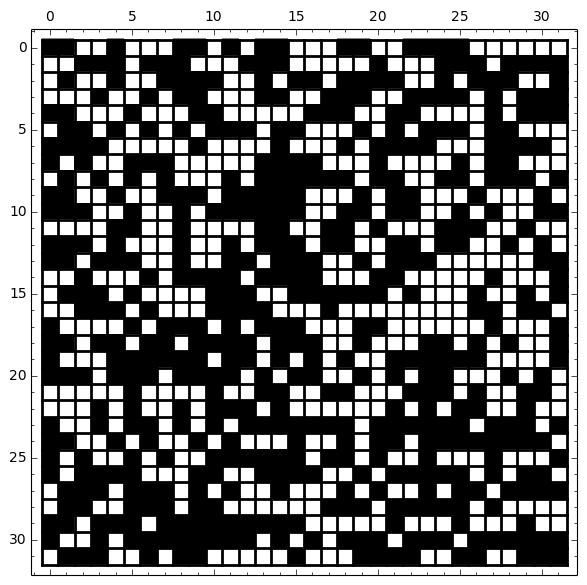
\includegraphics[scale=0.5]{figures/BC_lfsr_ex1.png}   %BERM0
\end{center}
\caption{Visualisierung der pseudozufälligen Bitfolge aus Abbildung~\ref{Sage-code-bool-psr},
   erzeugt mit dem SageMath-Beispiel~\ref{Sage-code-bool-psr}
   (1 = schwarz, 0 = weiß)}\label{fig-bool-lfsr2}
\end{figure}
\clearpage

\subsection{Algebraischer Angriff\index{algebraischer Angriff}\index{Angriff!algebraisch}
            auf lineare Schieberegister}\label{ss-bool-alg2}

Auch einfache Zufallsgeneratoren\index{Zufallsgenerator} wie die linearen
Schieberegister\index{lineares Schieberegister}\index{Schieberegister!linear} liefern,
wie gesehen, Bitfolgen, die mit statistischen Mitteln nicht ohne weiteres
von "`echtem"' Zufall unterschieden werden können und für statistische
Methoden der Kryptoanalyse keinen unmittelbar erfolgversprechenden
Ansatz bieten. Anders sieht es aus, wenn man
bekannten Klartext\index{bekannter Klartext}\index{Klartext!bekannt} annimmt
-- dann erhält man Gleichungen für die Schlüsselbits. Werden die
Schlüsselbits nach einem einfachen Algorithmus erzeugt, kann man
mit algebraischer
Kryptoanalyse\index{algebraische Kryptoanalyse}\index{Kryptoanalyse!algebraisch},
d.\,h. durch Auflösung dieser Gleichungen, auf Erfolg hoffen. Dies ist besonders
für lineare Schieberegister\footnote{%
  Die "`Rückkopplung"' wird in der Bezeichnungsweise meistens weggelassen,
  wenn keine Missverständnisse zu befürchten sind, ist hier aber implizit
  immer mit gemeint.
} der Fall.

Nehmen wir an, ein lineares
Schieberegister\index{lineares Schieberegister}\index{Schieberegister!linear}
hat den Schlüsselbitstrom $u_0, u_1, \ldots$ nach den
Formeln~(\ref{eq-bool-lfsr1}) und (\ref{eq-bool-lfsr2}) erzeugt.
Mit diesem Schlüsselstrom\index{Schlüsselstrom} wurde ein
Klartext $a$ per XOR\index{XOR}\index{Verschlüsselung!XOR}
zum Geheimtext $c$ verschlüsselt, $c_i = a_i + u_i$
für $i = 0, 1, \ldots$ Was kann die Gegnerin erreichen, wenn sie ein
Stück vom Anfang des Klartexts kennt?

Nun, kennt sie die ersten $l+1$ Bits des Klartexts, so hat sie sofort
die entsprechenden Bits $u_0, \ldots, u_l$ des Schlüsselstroms,
insbesondere den Startwert. Für die noch unbekannten Koeffizienten
$s_i$ kennt sie eine lineare Relation:
\[
     s_1 u_{l-1} + \cdots + s_l u_0 = u_l.
\]
Jedes weitere bekannte Bit des Klartexts liefert eine weitere Relation,
und mit $l$ solchen Relationen, also insgesamt $2l$ Bits an bekanntem
Klartext, liefert die sehr einfache Lineare
Algebra\index{lineare Algebra}\index{Algebra!lineare} über dem Körper
$\F_2$ im allgemeinen eine eindeutige Lösung. Die
$l \times l$-Koeffizientenmatrix dieses linearen
Gleichungssystems\index{lineares Gleichungssystem}\index{Gleichungssystem!linear}
ist im Wesentlichen die Matrix $U$ des nächsten Abschnitts. Ein
kleiner Umweg macht die Lösung noch ein wenig eleganter -- in den nächsten,
etwas mehr Mathematik voraussetzenden Abschnitten wird bewiesen:

\begin{satz}\label{thm-bool-lfsr}
  Ein lineares Schieberegister\index{lineares Schieberegister}\index{Schieberegister!linear}
  der Länge $l$ ist aus den ersten $2l$ Bits
  vorhersagbar. Der Aufwand dazu beträgt ungefähr $\frac{1}{3} \cdot l^3$
  Bitoperationen.
\end{satz}

\subsubsection*{Vorhersage linearer Schieberegister}

Nehmen wir an, wir kennen die ersten $2l$ Bits $u_0, \ldots, u_{2l-1}$
aus einem linearen Schieberegister\index{lineares Schieberegister}\index{Schieberegister!linear}
der Länge $l$. Die Lineare Algebra lässt
sich eleganter formulieren, wenn man die {\bf Zustandsvektoren\index{Zustandsvektor}}
\[
     u_{(i)} = (u_i, \ldots, u_{i+l-1}) \quad \text{für } i = 0, 1, \ldots
\]
verwendet. Dabei ist $u_{(i)}$ gerade der Inhalt des Registers beim Schritt
Nummer $i$ (in umgekehrter Reihenfolge) -- d.\,h., die Analyse konzentriert
sich nicht auf den Output, sondern setzt bei den Zuständen an. Die
Rekursionsformel~(\ref{eq-bool-lfsr1}) kann man dann für $n \geq l$ in
Matrixform als
\[
     \begin{pmatrix} u_{n-l+1} \\ \vdots \\ u_{n-1} \\ u_{n} \end{pmatrix}
     =
     \begin{pmatrix} 0      & 1      & \ldots & 0      \\
                     \vdots & \vdots & \ddots & \vdots \\
                     0      & 0      & \ldots & 1      \\
                     s_l    & s_{l-1}    & \ldots & s_1 \end{pmatrix}
     \begin{pmatrix} u_{n-l} \\ \vdots \\ u_{n-2} \\ u_{n-1} \end{pmatrix}
\]
schreiben oder sehr knapp und übersichtlich in der Form (mit substituierten Indizes
$m = n-l+1$)
\[
     u_{(m)} = S \cdot u_{(m-1)} \quad \text{für } m \geq 1\,,
\]
wobei $S$ die Koeffizientenmatrix ist. Noch einen Schritt weiter gehend
fasst man $l$ aufeinanderfolgende Zustandsvektoren
$u_{(i)}, \ldots, u_{(i+l-1)}$ zu einer Zustandsmatrix
\[
     U_{(i)} = \begin{pmatrix} u_i      & u_{i+1}      & \ldots & u_{i+l-1}      \\
                               u_{i+1} & u_{i+2} & \ldots & u_{i+l} \\
                               \vdots  & \vdots & \ddots & \vdots     \\
                     u_{i+l-1}    & u_{i+l} & \ldots & u_{2l-2} \end{pmatrix}
\]
zusammen, setzt $U = U_{(0)}$, $V = U_{(1)}$, und erhält damit die Formel
\[
     V  =  S \cdot U,
\]
die die unbekannten Koeffizienten $s_1, \ldots, s_l$ durch die bekannten
Klartextbits $u_0, \ldots, u_{2l-1}$ ausdrückt. Vor allem aber gestattet sie,
als Lohn für die Bemühungen sofort die Lösung hinzuschreiben -- vorausgesetzt,
die Matrix $U$ ist invertierbar:
\[
     S  =  V \cdot U^{-1},
\]
denn aus der Matrix $S$ kann man ja die Koeffizienten $s_j$ auslesen.
Mehr zur Invertierbarkeit später.

\subsubsection*{Beispiel}

Wir haben einen Geheimtext vorliegen:
\begin{verbatim}
   10011100 10100100 01010110 10100110 01011101 10101110
   01100101 10000000 00111011 10000010 11011001 11010111
   00110010 11111110 01010011 10000010 10101100 00010010
   11000110 01010101 00001011 11010011 01111011 10110000
   10011111 00100100 00001111 01010011 11111101
\end{verbatim}
Wir vermuten, dass er XOR-chiffriert\index{XOR}\index{Verschlüsselung!XOR}
ist mit einem Schlüsselstrom, der
durch ein lineares Schieberegister der Länge $l = 16$ erzeugt wurde.
Der Kontext lässt vermuten, dass der Text mit dem Wort "`Treffpunkt"'
beginnt. Zum Brechen benötigen wir nach der Theorie 32 Bits, also
nur die ersten vier Buchstaben. Daraus ermitteln wir 32 Bits des
Schlüsselstroms:
\begin{verbatim}
    01010100 01110010 01100101 01100110 = T r e f
    10011100 10100100 01010110 10100110   cipher bits
    -------- -------- -------- --------
    11001000 11010110 00110011 11000000   key bits
\end{verbatim}
Im SageMath-Beispiel~\ref{Sage-code-bool-lfsr2} wird die Koeffizientenmatrix
bestimmt. Die letzte Zeile sagt uns, dass die $s_i = 0$ sind außer
$s_{16} = s_5 = s_3 = s_2 = 1$.

Damit kennen wir das Schieberegister und den Startwert, können den
gesamten Schlüsselstrom berechnen -- ja, es ist der aus Abbildung~\ref{Sage-code-bool-psr}
-- und damit den Klartext herstellen
(der übrigens nicht ganz so beginnt wie vermutet).

\begin{sagecode}
\begin{verbatim}

sage: l = 16
sage: kbits =
      [1,1,0,0,1,0,0,0,1,1,0,1,0,1,1,0,0,0,1,1,0,0,1,1,1,1,0,0,0,0,0,0]
sage: ulist = []
sage: for i in range(0,l):
        state = kbits[i:(l+i)]
        ulist.append(state)
sage: U = matrix(GF(2),ulist)
sage: det(U)
1
sage: W = U.inverse()
sage: vlist = []
sage: for i in range(1,l+1):
        state = kbits[i:(l+i)]
        vlist.append(state)
sage: V = matrix(GF(2),vlist)
sage: S = V*W
sage: S
[0 1 0 0 0 0 0 0 0 0 0 0 0 0 0 0]
[0 0 1 0 0 0 0 0 0 0 0 0 0 0 0 0]
[0 0 0 1 0 0 0 0 0 0 0 0 0 0 0 0]
[0 0 0 0 1 0 0 0 0 0 0 0 0 0 0 0]
[0 0 0 0 0 1 0 0 0 0 0 0 0 0 0 0]
[0 0 0 0 0 0 1 0 0 0 0 0 0 0 0 0]
[0 0 0 0 0 0 0 1 0 0 0 0 0 0 0 0]
[0 0 0 0 0 0 0 0 1 0 0 0 0 0 0 0]
[0 0 0 0 0 0 0 0 0 1 0 0 0 0 0 0]
[0 0 0 0 0 0 0 0 0 0 1 0 0 0 0 0]
[0 0 0 0 0 0 0 0 0 0 0 1 0 0 0 0]
[0 0 0 0 0 0 0 0 0 0 0 0 1 0 0 0]
[0 0 0 0 0 0 0 0 0 0 0 0 0 1 0 0]
[0 0 0 0 0 0 0 0 0 0 0 0 0 0 1 0]
[0 0 0 0 0 0 0 0 0 0 0 0 0 0 0 1]
[1 0 0 0 0 0 0 0 0 0 0 1 0 1 1 0]
\end{verbatim}
\caption{Bestimmung einer Koeffizientenmatrix}\label{Sage-code-bool-lfsr2}
\end{sagecode}

\subsubsection*{Beweis des Satzes}

Für den Fall, dass die Zustandsmatrix $U = U_{(0)}$ invertierbar ist,
haben wir oben schon gezeigt, dass die Koeffizienten eindeutig bestimmbar sind.
Insbesondere ist dann das Schieberegister bekannt und aller weitere Output
vorhersagbar. Wir müssen uns also noch mit der Möglichkeit auseinandersetzen,
dass die Matrix $U$ nicht invertierbar sein könnte.

Falls einer der ersten $l$ Zustandsvektoren (= Zeilen der Matrix $U$)
Null ist, sind auch alle weiteren Null, die Vorhersage ist also trivial.

Wir können also annehmen, dass diese Vektoren alle nicht Null, aber linear
abhängig sind. Dann gibt es einen kleinsten Index $k \geq 1$, so dass
$u_{(k)}$ in dem von $u_{(0)}, \ldots, u_{(k-1)}$ aufgespannten
Unterraum liegt. D.\,h., es gibt Koeffizienten $t_1, \ldots, t_k \in \F_2$ mit
\[
     u_{(k)}  =  t_1 u_{(k-1)} + \cdots + t_k u_{(0)}.
\]
Dann gilt aber auch $u_{(k+1)} = S\cdot u_{(k)} =
t_1 S\cdot u_{(k-1)} + \cdots + t_k S\cdot u_{(0)} =
t_1 u_{(k)} + \cdots + t_k u_{(1)}$ und weiter durch Induktion
\[
     u_{(n)}  =  t_1 u_{(n-1)} + \cdots + t_k u_{(n-k)}
     \quad \text{für alle } n \geq k.
\]
Durch diese Formel werden also auch alle weiteren Bits vorhergesagt.

Die Aussage über den Aufwand folgt aus Satz~\ref{thm-bool-lin}.

\begin{description}
   \item[Diskussion:] ~
      \begin{itemize}
         \item Diese Überlegung ergibt für den Fall einer nicht invertierbaren
            Zustandsmatrix ein kürzeres lineares Schieberegisters (der Länge
            $k < l$), das die gleiche Folge erzeugt. In diesem Fall werden
            die Koeffizienten des originalen Registers also nicht bestimmt,
            aber die weitere Folge trotzdem korrekt vorhergesagt.
         \item Wenn nicht die ersten Bits, sondern $2l$ zusammenhängende
            Bits an späterer Stelle bekannt sind, ergibt der Satz zunächst
            nur eine Berechnung der späteren Bits. Im Regelfall, wo die
            Zustandsmatrix $U$ invertierbar ist, ist das Register aber
            dann völlig bekannt und kann natürlich auch rückwärts zur
            Bestimmung der Vorgängerbits eingesetzt werden. Ist die
            Zustandsmatrix nicht invertierbar, kann man das gleiche mit dem
            eben konstruierten kürzeren linearen Schieberegister erreichen.
         \item Etwas komplizierter wird die Situation, wenn man zwar $2l$
            Bits des Schlüsselstroms kennt, diese aber nicht zusammenhängen.
            Auch dann erhält man lineare Relationen, in denen aber
            zusätzlich unbekannte Zwischenbits vorkommen. Ist $m$ die Zahl
            der Lücken, so hat man dann insgesamt $l+m$ lineare Gleichungen
            für $l+m$ unbekannte Bits.
         \item Was aber, wenn auch die Länge $l$ des Registers unbekannt ist?
            Das Durchprobieren aller Werte $l = 1, 2, 3, \ldots$ ist sicher
            lästig, aber machbar. Es gibt aber auch den Algorithmus von
            Berlekamp-Massey\footnote{%
            in SageMath als {\tt sage.crypto.lfsr.berlekamp\_massey} enthalten,
            in CrypTool\,2 unter
            "`Kryptoanalyse"'/"`Generisch"'/"`Berlekamp-Massey-Algorithmus"'
            zu finden
            }, der ohne vorherige Kenntnis
            von $l$ sehr effizient ist. Dessen Behandlung würde aber hier
            zu weit führen.
      \end{itemize}
\end{description}

\subsubsection*{Fazit}

Kryptoanalyse bedeutet für Zufallsgeneratoren\index{Zufallsgenerator} wie in Abbildung~\ref{fig-bool-prg},
aus einem Teil ihres Outputs eine der folgenden Informationen zu bestimmen:
\begin{itemize}
\item die geheimen Parameter,
\item den Startwert,
\item weitere Teile des Outputs ("`Vorhersageproblem\index{Vorhersageproblem}"').
\end{itemize}
Wie wir bei den linearen
Schieberegistern\index{lineares Schieberegister}\index{Schieberegister!linear}
gesehen haben, ist es
realistisch, das Vorhersageproblem anzugehen, das auch lösbar sein
kann, wenn die Bestimmung der internen Parameter nicht gelingt.
Wir halten fest:
\begin{quote}
   {\em Die Kryptoanalyse eines Zufallsgenerators bedeutet in erster Linie
   die Lösung des Vorhersageproblems. Ein Zufallsgenerator\index{Zufallsgenerator}
   ist kryptographisch
   sicher, wenn sein Vorhersageproblem nicht effizient lösbar ist.}
\end{quote}

\begin{quote}
   {\em Lineare Schieberegister\index{lineares Schieberegister}\index{Schieberegister!linear}
   sind kryptographisch nicht sicher.}
\end{quote}

\subsection{Nichtlinearität\index{Nichtlinearität} für Schieberegister
   -- Ansätze}\label{ss-bool-nlsr}

Lineare Schieberegister sind beliebt -- vor allem bei Elektro-Ingenieuren
und beim Militär -- denn sie sind
\begin{itemize}
	\item sehr einfach zu realisieren,
	\item extrem effizient in Hardware,
	\item als Zufallsgeneratoren für statistische Zwecke sehr gut geeignet,
	\item problemlos in großer Anzahl parallel zu betreiben,
	\item aber leider kryptologisch völlig unsicher.
\end{itemize}
Um die positiven Eigenschaften zu nutzen und die kryptologische Schwäche
zu vermeiden, gibt es verschiedene Ansätze.

\subsubsection*{Ansatz 1: Nichtlineare Rückkopplung}

Die nichtlineare Rückkopplung\index{Rückkopplung}
folgt dem Schema aus Abbildung~\ref{fig-bool-fsr}
mit einer nichtlinearen Booleschen Funktion\index{Boolesche
Funktion}\index{Funktion!Boolesche} $f$.
Sie wird hier nicht weiter behandelt; ein ganz
einfaches, kryptographisch ungeeignetes Beispiel war das
SageMath-Beispiel~\ref{Sage-code-bool-fsr1}. Man kann aber auch
allgemein zeigen, dass solche nichtlinearen Schieberegister
(nonlinear feedback, NLFSR\footnote{%
   für Non-Linear Feedback Shift Register\index{Schieberegister!nichtlinear}
}
), für sich allein genommen, unter realistischen Annahmen
im praktischen Einsatz nicht kryptographisch
sicher sind \cite{Pom2016}.


\subsubsection*{Ansatz 2: Nichtlinearer Ausgabefilter}

Der nichtlineare Ausgabefilter\index{Ausgabefilter}
(Non-Linear Feedforward) folgt dem Schema
aus Abbildung~\ref{fig-bool-nlf}.
Das Schieberegister selbst ist linear. Der nichtlineare Ausgabefilter
ist ein Spezialfall des nächsten Ansatzes.

\begin{figure}
\begin{center}
\begin{picture}(320,150)
  \linethickness{2pt}
  \put(20,20){\line(1,0){260}}
  \put(20,20){\line(0,1){30}}
  \put(20,50){\line(1,0){260}}
  \put(280,20){\line(0,1){30}}
  \put(260,120){\circle{30}}
  \put(256,117){$f$}

  \linethickness{1pt}
  \put(60,20){\line(0,1){30}}
  \put(100,20){\line(0,1){30}}
  \put(240,20){\line(0,1){30}}
  \put(200,20){\line(0,1){30}}
  \put(110,30){\ldots}
  \put(180,30){\ldots}

  \put(40,20){\line(0,-1){20}}
  \put(80,20){\line(0,-1){20}}
  \put(220,20){\line(0,-1){20}}
  \put(260,20){\line(0,-1){20}}
  \put(260,0){\line(-1,0){260}}
  \put(0,0){\line(0,1){35}}
  \put(0,35){\vector(1,0){20}}

  \put(260,50){\vector(0,1){53}}
  \put(220,50){\vector(1,2){29}}
  \put(80,50){\line(0,1){25}}
  \put(80,75){\vector(4,1){163}}
  \put(40,50){\line(0,1){70}}
  \put(40,120){\vector(1,0){203}}

  \put(277,120){\vector(1,0){43}}
\end{picture}
\end{center}
\caption{Nichtlinearer Ausgabefilter für ein lineares Schieberegister}\label{fig-bool-nlf}
\end{figure}

\subsubsection*{Ansatz 3: Nichtlinearer Kombinierer\index{Kombinierer}}

Hier wird eine "`Batterie"' aus $n$ linearen Schieberegistern -- die durchaus
unterschiedliche Länge haben können und sollen -- parallel betrieben.
Ihre Outputfolgen werden in eine
Boolesche Funktion\index{Boolesche Funktion}\index{Funktion!Boolesche}
$f\!\!: \F_2^n \longrightarrow \F_2$ gefüttert\footnote{%
   daher auch hierfür gelegentlich die Bezeichnung Non-Linear Feedforward
}, siehe Abbildung~\ref{fig-bool-nlc}.
Ein Ansatz zur Analyse dieses Verfahrens folgt in Abschnitt~\ref{ss-bool-bsana}.

\begin{figure}
\begin{center}
\begin{picture}(350,200)
  \linethickness{2pt}
  \put(20,20){\line(1,0){260}}
  \put(20,20){\line(0,1){30}}
  \put(20,50){\line(1,0){260}}
  \put(280,20){\line(0,1){30}}

  \linethickness{1pt}
  \put(60,20){\line(0,1){30}}
  \put(100,20){\line(0,1){30}}
  \put(240,20){\line(0,1){30}}
  \put(200,20){\line(0,1){30}}
  \put(110,30){\ldots}
  \put(180,30){\ldots}

  \put(40,20){\line(0,-1){20}}
  \put(80,20){\line(0,-1){20}}
  \put(220,20){\line(0,-1){20}}
  \put(260,20){\line(0,-1){20}}
  \put(260,0){\line(-1,0){260}}
  \put(0,0){\line(0,1){35}}
  \put(0,35){\vector(1,0){20}}

  \linethickness{2pt}
  \put(20,150){\line(1,0){260}}
  \put(20,150){\line(0,1){30}}
  \put(20,180){\line(1,0){260}}
  \put(280,150){\line(0,1){30}}

  \linethickness{1pt}
  \put(60,150){\line(0,1){30}}
  \put(100,150){\line(0,1){30}}
  \put(240,150){\line(0,1){30}}
  \put(200,150){\line(0,1){30}}
  \put(110,160){\ldots}
  \put(180,160){\ldots}

  \put(40,150){\line(0,-1){20}}
  \put(80,150){\line(0,-1){20}}
  \put(220,150){\line(0,-1){20}}
  \put(260,150){\line(0,-1){20}}
  \put(260,130){\line(-1,0){260}}
  \put(0,130){\line(0,1){35}}
  \put(0,165){\vector(1,0){20}}

  \put(80,100){$\vdots$}
  \put(220,100){$\vdots$}
  \put(80,70){$\vdots$}
  \put(220,70){$\vdots$}

  \put(280,165){\vector(1,0){20}}
  \put(280,35){\vector(1,0){20}}
  \put(315,100){\oval(30,160)}
  \put(330,100){\vector(1,0){20}}
  \put(313,97){$f$}
\end{picture}
\end{center}
\caption{Nichtlinearer Kombinierer}\label{fig-bool-nlc}
\end{figure}

\subsubsection*{Ansatz 4: Auswahlsteuerung/Dezimierung/Taktung}

Weitere Möglichkeiten bestehen in verschiedenen Methoden zur Steuerung
einer Batterie von $n$ parallel betriebenen linearen Schieberegistern
durch ein weiteres lineares Schieberegister:
\begin{itemize}
	\item Bei der {\bf Auswahlsteuerung}\index{Auswahlsteuerung}
        wird je nach Zustand des "`Hilfsregisters"'
	   das aktuelle Output-Bit von genau einem der "`Batterie-Register"' als
	   Output des Zufallsgenerators ausgewählt. Allgemeiner kann man auch
	   eine Auswahl "`$r$ aus $n$"' treffen.
	\item Bei der {\bf Dezimierung}\index{Dezimierung} nimmt man
        im allgemeinen $n = 1$ an und gibt das
	   Output-Bit des einen Batterie-Registers nur dann aus, wenn das
	   Hilfsregister einen bestimmten Zustand hat. Diese Art der Dezimierung
	   kann man natürlich analog auf jede Bitfolge anwenden.
	\item Bei der {\bf Taktung}\index{Taktung} gibt der Zustand
        des Hilfsregisters an, welche
	   der Batterie-Register im aktuellen Taktzyklus weitergeschoben werden
	   (und um wie viele Positionen) und welche in ihrem momentanen Zustand bleiben.
	   Das ist vergleichbar mit der Steuerlogik von
        Rotor-Maschinen\index{Rotor-Maschine}.
\end{itemize}
Diese Ansätze lassen sich oft bequem auch als nichtlineare Kombinierer schreiben,
so dass Ansatz 3 als der gängigste Ansatz zur Rettung der linearen
Schieberegister\index{lineares Schieberegister}\index{Schieberegister!linear}
angesehen werden kann.

Der Mobilfunk-Verschlüsselungsstandard
\href{http://de.wikipedia.org/wiki/A5\_(Algorithmus)}{A5/1}\index{A5}  %% Ok in PDF, aber 1. in href muss man "_" maskieren, was unschön ist. 2. Wie sichtbar machen, dass hinter "A5/1" eine URL, auf die man tippen kann und die einen Balloontext hat. Ich habe urlcolor=cyan gesetzt. Gibt es etwas Eleganteres und etwas, was man im s/w-Ausdruck besser sieht (black und blue sieht man gut)? ==> Todo Doris
% yyy \href{\url{http://de.wikipedia.org/wiki/A5_(Algorithmus)}}{A5/1}\index{A5}  %% lässt sich nicht compilieren
% yyy \url{http://de.wikipedia.org/wiki/A5_(Algorithmus)}{A5/1}\index{A5}  %% Gibt URL aus
verwendet drei leicht unterschiedlich getaktete lineare Schieberegister
der Längen 19, 22 und 23 mit jeweils maximaler Periode, deren
Outputströme linear (nämlich einfach durch binäre Addition)
kombiniert werden. Bei A5/2 -- das noch schwächer ist -- wird
die Taktung durch ein Hilfsregister geregelt. Beide Varianten
lassen sich auf handelsüblichen PCs in Echtzeit brechen.

Der Bluetooth-Verschlüsselungsstandard $\mathrm{E}_0$\index{E0} verwendet vier
lineare Schieberegister, die nichtlinear kombiniert werden. Dieses Verfahren
ist etwas stärker als A5, aber auch zu schwach für echte Sicherheit \cite{Schm2016}.

\subsubsection*{Beispiel: Der Geffe-Generator}

Das einfachste Beispiel für die Auswahlsteuerung ist der
Geffe-Generator\index{Geffe-Generator},
der durch das Schema in Abbildung~\ref{fig-bool-gef}
beschrieben wird. Die Ausgabe ist $x$, wenn $z = 0$, und $y$, wenn
$z = 1$. Das kann man so als Formel ausdrücken:
\begin{eqnarray*}
   u & = & \begin{cases}
              x, & \text{wenn } z = 0, \\
              y, & \text{wenn } z = 1
           \end{cases} \\
      & = & (1 - z) x + zy = x + zx + zy.
\end{eqnarray*}
Also lässt sich der Geffe-Generator auch durch einen nichtlinearen
Kombinierer mit einer Booleschen Funktion
$f\!\!: \F_2^3 \longrightarrow \F_2$ vom Grad 2 beschreiben. Diese
wird zur späteren Verwendung im SageMath-Beispiel~\ref{Sage-code-bool-gef}
erzeugt.

\begin{figure}
\begin{center}
\setlength{\unitlength}{1pt}
\begin{picture}(350,200)
  \linethickness{2pt}
  \put(20,20){\line(1,0){260}}
  \put(20,20){\line(0,1){30}}
  \put(20,50){\line(1,0){260}}
  \put(280,20){\line(0,1){30}}

  \linethickness{1pt}
  \put(60,20){\line(0,1){30}}
  \put(100,20){\line(0,1){30}}
  \put(240,20){\line(0,1){30}}
  \put(200,20){\line(0,1){30}}
  \put(110,30){\ldots}
  \put(180,30){\ldots}

  \put(40,20){\line(0,-1){20}}
  \put(80,20){\line(0,-1){20}}
  \put(220,20){\line(0,-1){20}}
  \put(260,20){\line(0,-1){20}}
  \put(260,0){\line(-1,0){260}}
  \put(0,0){\line(0,1){35}}
  \put(0,35){\vector(1,0){20}}

  \linethickness{2pt}
  \put(20,80){\line(1,0){260}}
  \put(20,80){\line(0,1){30}}
  \put(20,110){\line(1,0){260}}
  \put(280,80){\line(0,1){30}}

  \linethickness{1pt}
  \put(60,80){\line(0,1){30}}
  \put(100,80){\line(0,1){30}}
  \put(240,80){\line(0,1){30}}
  \put(200,80){\line(0,1){30}}
  \put(110,90){\ldots}
  \put(180,90){\ldots}

  \put(40,80){\line(0,-1){20}}
  \put(80,80){\line(0,-1){20}}
  \put(220,80){\line(0,-1){20}}
  \put(260,80){\line(0,-1){20}}
  \put(260,60){\line(-1,0){260}}
  \put(0,60){\line(0,1){35}}
  \put(0,95){\vector(1,0){20}}

  \linethickness{2pt}
  \put(50,160){\line(1,0){260}}
  \put(50,160){\line(0,1){30}}
  \put(50,190){\line(1,0){260}}
  \put(310,160){\line(0,1){30}}

  \linethickness{1pt}
  \put(90,160){\line(0,1){30}}
  \put(130,160){\line(0,1){30}}
  \put(270,160){\line(0,1){30}}
  \put(230,160){\line(0,1){30}}
  \put(140,170){\ldots}
  \put(210,170){\ldots}

  \put(70,160){\line(0,-1){20}}
  \put(110,160){\line(0,-1){20}}
  \put(250,160){\line(0,-1){20}}
  \put(290,160){\line(0,-1){20}}
  \put(290,140){\line(-1,0){260}}
  \put(30,140){\line(0,1){35}}
  \put(30,175){\vector(1,0){20}}

  \put(310,175){\line(1,0){20}}
  \put(330,175){\line(0,-1){40}}
  \put(333,152){$z$}
  \put(330,135){\line(-1,0){15}}
  \put(315,135){\vector(0,-1){25}}

  \put(280,95){\vector(1,0){20}}
  \put(288,97){$x$}
  \put(280,35){\vector(1,0){20}}
  \put(288,38){$y$}
  \put(315,65){\oval(30,90)}
  \put(330,65){\line(-1,-1){30}}
  \put(330,65){\vector(1,0){20}}
\end{picture}
\end{center}
\caption{Geffe-Generator}\label{fig-bool-gef}
\end{figure}

\begin{sagecode}
\begin{verbatim}

sage: geff = BoolF(str2bbl("00011100"),method="ANF")
sage: geff.printTT()
Value at 000 is 0
Value at 001 is 0
Value at 010 is 0
Value at 011 is 1
Value at 100 is 1
Value at 101 is 0
Value at 110 is 1
Value at 111 is 1
\end{verbatim}
\caption{Die Geffe-Funktion}\label{Sage-code-bool-gef}
\end{sagecode}

\subsection{Implementation eines nichtlinearen Kombinierers}\label{ss-bool-ncsr}

Ein nichtlinearer Kombinierer\index{Kombinierer} benötigt mehrere parallel betriebene
lineare Schieberegister. Dies legt nahe, diese als Objekte zu
implementieren, d.\,h., eine Klasse {\tt LFSR} zu definieren\footnote{%
   siehe auch in CrypTool\,2 unter "`Protokolle"'/"`LFSR"' bzw. "`NLFSR"'
}.

\begin{description}
   \item[Klasse {\tt LSFR}:] ~
      \begin{description}
         \item[Attribute:] ~
            \begin{itemize}
               \item {\tt length}: die Länge des Registers
               \item {\tt taplist}: die Liste der Koeffizienten ("`Taps"'\footnote{%
                    auf deutsch etwa "`Abzweig"' oder "`Abgriff"', weil bei einer
                    Hardware-Implementierung genau an diesen Stellen die für die
                    Rückkopplung verwendeten Bits abgegriffen werden
                  }), die die  rückzukoppelnden Bits definieren (konstant)
               \item {\tt state}: der Zustand des Registers (veränderbar)
            \end{itemize}
         \item[Methoden:] ~
            \begin{itemize}
               \item {\tt setLength}: Definition der Länge (nur implizit bei
                  der Initialisierung verwendet)
               \item {\tt setTaps}: Besetzung der Tap- (= Koeffizienten-) Liste
                  (nur implizit bei der Initialisierung verwendet)
               \item {\tt setState}: Belegung des Registers mit einem Zustand
               \item {\tt getLength}: Ausgabe der Länge
               \item {\tt nextBits}: Erzeugung einer vorgegebenen Anzahl von
                  Ausgabebits und kontinuierliche Weiterschaltung des Zustands
            \end{itemize}
      \end{description}
\end{description}
Dazu ist es zur Überwachung des Registers praktisch, noch eine Methode
(die in Python\index{Python} generisch {\tt \_\_str\_\_} heißt) zu haben, die die
Attribute in lesbarer Form ausgibt.

Für die Implementation siehe das SageMath-Beispiel~\ref{Sage-code-bool-lfsr3}
im Abschnitt~\ref{ss-bool-lfsrclass}.

\subsubsection*{Beispiel: Geffe-Generator\index{Geffe-Generator}}

Zunächst wählen wir drei lineare Schieberegister der Längen 15, 16 und 17,
deren Perioden\footnote{%
  nach den Listen primitiver Polynome in \cite{Menezes2001}
} $2^{15} - 1 = 32767$, $2^{16} - 1 = 65535$ und
$2^{17} - 1 = 131071$ sind, und diese sind paarweise teilerfremd, siehe
SageMath-Beispiel~\ref{Sage-code-bool-per}.
Fasst man ihren Output in jedem Takt zu Bitblöcken der Länge $3$
zusammen, so hat diese Folge eine Periode der eindrucksvollen Länge
$281459944554495$, also knapp $300 \times 10^{12}$ (300 Billionen\footnote{%
  europäische Billionen. Amerikanisch wären das 300 Trillionen.
}).
Die drei Register werden im SageMath-Beispiel~\ref{Sage-code-bool-regs}
definiert; die Rekursionsformel für das dritte davon, das
Steuerungsregister {\tt reg17}, ist z.\,B. $u_n = u_{n-3} + u_{n-17}$,
da genau die Taps 3 und 17 gesetzt sind.
Mit jedem von ihnen wird eine Folge der Länge 100 erzeugt,
siehe SageMath-Beispiel~\ref{Sage-code-bool-seqs}. Diese werden im
SageMath-Beispiel~\ref{Sage-code-bool-gef-seq} mithilfe der
Geffe-Funktion kombiniert.

\begin{sagecode}
\begin{verbatim}

sage: n15 = 2**15 - 1; n15
32767
sage: n15.factor()
7 * 31 * 151
sage: n16 = 2**16 - 1; n16
65535
sage: n16.factor()
3 * 5 * 17 * 257
sage: n17 = 2**17 - 1; n17
131071
sage: n17.factor()
131071
sage: period = n15 * n16 * n17; period
281459944554495
\end{verbatim}
\caption{Eine Periodenberechnung}\label{Sage-code-bool-per}
\end{sagecode}

\begin{sagecode}
\begin{verbatim}

sage: reg15 = LFSR([1,0,0,0,0,0,0,0,0,0,0,0,0,0,1])
sage: reg15.setState([0,1,1,0,1,0,1,1,0,0,0,1,0,0,1])
sage: print(reg15)
Length: 15 | Taps: 100000000000001 | State: 011010110001001
sage: reg16 = LFSR([0,1,1,0,1,0,0,0,0,0,0,0,0,0,0,1])
sage: reg16.setState([0,1,1,0,1,0,1,1,0,0,0,1,0,0,1,1])
sage: print(reg16)
Length: 16 | Taps: 0110100000000001 | State: 0110101100010011
sage: reg17 = LFSR([0,0,1,0,0,0,0,0,0,0,0,0,0,0,0,0,1])
sage: reg17.setState([0,1,1,0,1,0,1,1,0,0,0,1,0,0,1,1,1])
sage: print(reg17)
Length: 17 | Taps: 00100000000000001 | State: 01101011000100111
\end{verbatim}
\caption{Drei lineare Schieberegister}\label{Sage-code-bool-regs}
\end{sagecode}

\begin{sagecode}
\begin{verbatim}

sage: nofBits = 100
sage: outlist15 = reg15.nextBits(nofBits)
sage: print(outlist15)
[1, 0, 0, 1, 0, 0, 0, 1, 1, 0, 1, 0, 1, 1, 0, 1, 1, 1, 0, 0,
 0, 0, 1, 0, 0, 1, 1, 0, 1, 1, 0, 1, 0, 0, 0, 0, 0, 1, 1, 1,
 0, 1, 1, 0, 1, 1, 0, 0, 0, 0, 0, 0, 1, 0, 1, 1, 0, 1, 1, 0,
 1, 1, 1, 1, 1, 1, 1, 0, 0, 1, 0, 0, 1, 0, 0, 1, 0, 1, 0, 1,
 0, 1, 1, 1, 0, 0, 0, 1, 1, 1, 0, 0, 1, 1, 0, 0, 1, 0, 1, 1]
sage: outlist16 = reg16.nextBits(nofBits)
sage: print(outlist16)
[1, 1, 0, 0, 1, 0, 0, 0, 1, 1, 0, 1, 0, 1, 1, 0, 0, 0, 1, 1,
 0, 0, 1, 1, 1, 1, 0, 0, 0, 0, 0, 0, 0, 0, 1, 1, 1, 0, 1, 1,
 1, 0, 0, 0, 1, 1, 1, 0, 0, 0, 0, 0, 1, 0, 0, 0, 1, 1, 1, 0,
 1, 1, 1, 1, 0, 1, 0, 0, 1, 0, 0, 1, 1, 1, 1, 0, 0, 1, 0, 1,
 1, 0, 1, 1, 1, 1, 0, 0, 1, 0, 1, 1, 1, 0, 0, 1, 0, 0, 0, 1]
sage: outlist17 = reg17.nextBits(nofBits)
sage: print(outlist17)
[1, 1, 1, 0, 0, 1, 0, 0, 0, 1, 1, 0, 1, 0, 1, 1, 0, 0, 0, 1,
 0, 0, 0, 0, 0, 0, 1, 1, 0, 0, 1, 1, 1, 1, 1, 1, 0, 1, 1, 0,
 1, 1, 0, 0, 0, 0, 0, 1, 1, 1, 0, 0, 0, 0, 1, 1, 0, 0, 0, 0,
 0, 0, 0, 0, 1, 1, 1, 1, 1, 1, 1, 0, 0, 1, 0, 0, 1, 0, 0, 1,
 0, 1, 0, 1, 0, 1, 0, 1, 1, 0, 0, 1, 0, 1, 1, 0, 0, 1, 1, 0]
\end{verbatim}
\caption{Drei LFSR-Folgen}\label{Sage-code-bool-seqs}
\end{sagecode}
\clearpage

\begin{sagecode}
\begin{verbatim}

sage: outlist = []
sage: for i in range(0,nofBits):
....:     x = [outlist15[i],outlist16[i],outlist17[i]]
....:     outlist.append(geff.valueAt(x))
....:
sage: print(outlist)
[1, 1, 0, 1, 0, 0, 0, 1, 1, 1, 0, 0, 0, 1, 1, 0, 1, 1, 0, 1,
 0, 0, 1, 0, 0, 1, 0, 0, 1, 1, 0, 0, 0, 0, 1, 1, 0, 0, 1, 1,
 1, 0, 1, 0, 1, 1, 0, 0, 0, 0, 0, 0, 1, 0, 0, 0, 0, 1, 1, 0,
 1, 1, 1, 1, 0, 1, 0, 0, 1, 0, 0, 0, 1, 1, 0, 1, 0, 1, 0, 1,
 0, 0, 1, 1, 0, 1, 0, 0, 1, 1, 0, 1, 1, 0, 0, 0, 1, 0, 0, 1]
\end{verbatim}
\caption{Die kombinierte Folge}\label{Sage-code-bool-gef-seq}
\end{sagecode}

\subsection{Korrelationsattacken\index{Korrelationsattacke}
    -- die Achillesferse der Kombinierer}\label{ss-bool-bsana}

Sei $f\!\!: \F_2^n \longrightarrow \F_2$ die Kombinierfunktion eines
nichtlinearen Kombinierers\index{Kombinierer}. Die Anzahl
\[
   K_f := \#\{ x = (x_1, \ldots, x_n) \in \F_2^n \:|\: f(x) = x_1 \}
\]
gibt an, wie oft der Funktionswert mit dem ersten Argument übereinstimmt.
Ist sie $> 2^{n-1}$, so ist die Wahrscheinlichkeit für diese Übereinstimmung,
\[
   p = \frac{1}{2^n} \cdot K_f > \frac{1}{2},
\]
also überdurchschnittlich. Die kombinierte Outputfolge "`korreliert"' also
stärker mit dem Output des ersten linearen Schieberegisters, als zufällig
zu erwarten wäre. Ist $p < \frac{1}{2}$, so weicht die Korrelation nach
unten vom zufälligen Wert ab.

Diesen Effekt kann sich die Kryptoanalytikerin bei einem Angriff mit
bekanntem Klartext\index{bekannter Klartext}\index{Klartext!bekannt}
zunutze machen. Angenommen wird, dass ihr die
"`Hardware"', also die Rekursionsformeln für die Register (die Taps) und
auch die Kombinierfunktion $f$, bekannt ist. Gesucht sind die als Schlüssel
betrachteten Startvektoren aller Register. Die Bits $k_0, \ldots, k_{r-1}$
des Schlüsselstroms\footnote{%
  Der Einfachheit der Darstellung halber die ersten $r$ -- für irgendwelche $r$
  bekannten Schlüsselbits funktioniert die Argumentation genauso.
} seien bekannt. Mit einer Exhaustion über die $2^{l_1}$
Startvektoren des ersten Registers erzeugt man jedesmal die Folge
$u_0, \ldots, u_{r-1}$ und zählt die Übereinstimmungen. Zu erwarten ist
\[
   \frac{1}{r}\cdot \#\{i \:|\: u_i = k_i\} \approx
   \begin{cases}
      p & \text{beim richtigen Startvektor,} \\
      \frac{1}{2} & \text{sonst.}
   \end{cases}
\]
Falls $r$ groß genug ist, kann man also den echten Startvektor des ersten
Registers mit einem Aufwand $\sim 2^{l_1}$ (mit hoher Wahrscheinlichkeit)
bestimmen. Macht man dann mit
den anderen Registern genauso weiter, gelingt die Identifikation des
gesamten Schlüssels mit einem Aufwand $\sim 2^{l_1} + \cdots + 2^{l_n}$.
Das ist zwar exponenziell, aber wesentlich geringer als der Aufwand
$\sim 2^{l_1} \cdots 2^{l_n}$ für die naive vollständige Schlüsselsuche.

In der Sprache der linearen
Kryptoanalyse\index{lineare Kryptoanalyse}\index{Kryptoanalyse!linear}
aus \ref{ss-bool-lka} haben
wir hier die lineare Relation\index{lineare Relation}\index{Relation!linear}
\[
     f(x_1, \ldots, x_n) \stackrel{p}{\approx} x_1
\]
für $f$ ausgenutzt. Klar ist, dass man analog jede lineare
Relation ausnutzen kann, um die Komplexität der vollständigen Schlüsselsuche
zu reduzieren\footnote{%
  Eine genauere Analyse der Situation führt auf den Begriff der
  Korrelationsimmunität\index{Korrelationsimmunität}, die mit dem linearen
  Potenzial\index{lineares Potenzial}\index{Potenzial!linear}
  verwandt ist.
}.

\subsubsection*{Korrelationen des Geffe-Generators}

Für den Geffe-Generator\index{Geffe-Generator} kann man die Korrelationen aus
der Wahrheitstafel, Tabelle~\ref{tab-bool-gef-wt}, ablesen:
Als Wahrscheinlichkeit für die Übereinstimmung erhält man also
\[
   p = \begin{cases}
          \frac{3}{4} & \text{für das Register 1 ($x$),} \\
          \frac{3}{4} & \text{für das Register 2 ($y$),} \\
          \frac{1}{2} & \text{für das Register 3 ($z =$ Steuerung).}
       \end{cases}
\]
Daher lassen sich bei einer Korrelationsattacke die Startwerte für die
Register 1 und 2 -- die Batterieregister -- leicht schon aus kurzen
Outputfolgen bestimmen; den Startwert für Register 3, das Steuerungsregister,
findet man dann auch leicht durch Exhaustion.

\begin{table}
\begin{center}
  \begin{tabular}{|c|cccc|cccc|}\hline
      $x$    & $0$ & $0$ & $0$ & $0$ & $1$ & $1$ & $1$ & $1$ \\
      $y$    & $0$ & $0$ & $1$ & $1$ & $0$ & $0$ & $1$ & $1$ \\
      $z$    & $0$ & $1$ & $0$ & $1$ & $0$ & $1$ & $0$ & $1$ \\
    \hline
  $f(x,y,z)$ & $0$ & $0$ & $0$ & $1$ & $1$ & $0$ & $1$ & $1$ \\
    \hline
  \end{tabular}
\end{center}
\caption{Wahrheitstafel der Geffe-Funktion (waagerecht angeordnet)}\label{tab-bool-gef-wt}
\end{table}

Diese Schwachstelle des Geffe-Generators wird im
SageMath-Beispiel~\ref{Sage-code-bool-gef-lp} nachvollzogen, das als
Fortsetzung des SageMath-Beispiels~\ref{Sage-code-bool-gef} einzugeben ist.
Da wir das lineare Profil nur in der Klasse {\tt BoolMap} definiert
haben, müssen wir zuerst die Funktion {\tt geff} als Boolesche
Abbildung interpretieren -- also als Liste der Länge 1 von Booleschen
Funktionen. Das lineare Profil wird als Matrix
mit 2 Spalten und 8 Zeilen gedacht. Die erste Spalte
{\tt [64, 0, 0, 0, 0, 0, 0, 0]} misst die Übereinstimmung mit der
Linearform 0 des Bildbereichs. Sie enthält also keine nennenswerte
Information, außer dass alles durch $64$ zu dividieren ist. Die
zweite Spalte {\tt [0, 0, 16, 16, 16, 16, 0, 0]} wird
(nach dieser Division) in der Tabelle~\ref{tab-bool-gef-korr}
als Liste der Korrelationswahrscheinlichkeiten $p$ interpretiert.
Dabei wird die Formel
\[
     p = \frac{1}{2} \cdot (\pm \sqrt{\lambda} + 1)
\]
verwendet. Ist $\lambda = 0$, so $p = 1/2$. Ist  $\lambda = 1/4$,
so $p = 1/4$ oder $3/4$. Die Entscheidung zwischen diesen beiden
Werten für $p$ kann man anhand der Tabelle~\ref{tab-bool-gef-wt}
treffen.

\begin{table}
\begin{center}
\begin{tabular}{|l|cccccccc|} \hline
  Linearform     & $0$   &   $z$   &   $y$    &   $y+z$   &  $x$    &   $x+z$   &  $x+y$  & $x+y+z$ \\
  Repräsentation & $000$ & $001$ & $010$ & $011$ & $100$ & $101$ & $110$ & $111$ \\ \hline
  Potenzial      & $0$   & $0$   & $1/4$ & $1/4$ & $1/4$ & $1/4$ & $0$   & $0$ \\
  Wahrsch. $p$   & $1/2$ & $1/2$ & $3/4$ & $1/4$ & $3/4$ & $3/4$ & $1/2$ & $1/2$ \\ \hline
\end{tabular}
\end{center}
\caption{Korrelationswahrscheinlichkeiten der Geffe-Funktion}\label{tab-bool-gef-korr}
\end{table}

\begin{sagecode}
\begin{verbatim}

sage: g = BoolMap([geff])
sage: linProf = g.linProf(); linProf
[[64, 0], [0, 0], [0, 16], [0, 16], [0, 16], [0, 16], [0, 0], [0, 0]]
\end{verbatim}
\caption{Lineares Profil der Geffe-Funktion}\label{Sage-code-bool-gef-lp}
\end{sagecode}

Im SageMath-Beispiel~\ref{Sage-code-bool-gef-coi} wird diese Erkenntnis auf
die mit dem Geffe-Generator erzeugte Folge der Länge $100$ angewendet.
Zur Zählung der Koinzidenzen (= Übereinstimmungen) wird die Funktion {\tt coinc} aus dem
SageMath-Beispiel~\ref{Sage-code-bool-div-bbl} (im Anhang) verwendet. Mit dem ersten
Register gibt es $73$, mit dem zweiten $76$ Koinzidenzen, mit dem
dritten dagegen nur $41$. Das passt sehr gut zu den im Rahmen statistischer Schwankungen
theoretisch erwarteten Werten $75$, $75$, $50$.

\begin{sagecode}
\begin{verbatim}

sage: coinc(outlist15,outlist)
73
sage: coinc(outlist16,outlist)
76
sage: coinc(outlist17,outlist)
41
\end{verbatim}
\caption{Koinzidenzen des Geffe-Generators}\label{Sage-code-bool-gef-coi}
\end{sagecode}

\subsubsection*{Analyse des Geffe-Generators\index{Geffe-Generator}}

Diese deutlichen Ergebnisse legen nahe, dass die Analyse der beispielhaft
erzeugten Folge leicht sein sollte. Für eine grobe Erfolgsabschätzung
kann man auf mathematische Strenge verzichten.

Betrachtet wird ein fest vorgegebener Bitblock $b \in \F_2^r$. Wir fragen
zunächst, wie groß die Wahrscheinlichkeit für einen zufälligen Bitblock
$u \in \F_2^r$ ist, an genau $t$ Stellen mit $b$ übereinzustimmen,
also $t$ Koinzidenzen zu haben. Das ist genau die Fragestellung der
symmetrischen Binomialverteilung\index{Binomialverteilung}
(also mit $p = \frac{1}{2}$ als
Wahrscheinlichkeit einer einzelnen Übereinstimmung): Die
Wahrscheinlichkeit für genau $t$ Koinzidenzen ist
\[
     B_{r,\frac{1}{2}}(t)  =  \frac{\binom{r}{t}}{2^r}.
\]
Die Wahrscheinlichkeit für bis zu $T$ Koinzidenzen ist also
\[
     \sum_{t=0}^T B_{r,\frac{1}{2}}(t)
       =  \frac{1}{2^r} \cdot \sum_{t=0}^T \binom{r}{t}.
\]
Wenn $r$ nicht zu groß ist, kann man diesen Wert für eine konkrete
Schranke $T$ explizit ausrechnen. Wenn $r$ nicht zu klein ist,
approximiert man ihn mithilfe der Normalverteilung\index{Normalverteilung}.
Dazu benötigt man den Erwartungswert für die
Anzahl der Koinzidenzen, der $r/2$ ist, die Varianz $r/4$ und die
Standardabweichung $\sqrt{r}/2$.

Wie auch immer man das macht, im Fall $r = 100$ ist (exemplarisch) die
Wahrscheinlichkeit, maximal $65$ Koinzidenzen zu finden, ziemlich
genau $0,999$, die Überschreitungswahrscheinlichkeit also
%%%  Da \textperthousand nicht funktionierte (auch nicht mit package textcomp), \permil genommen.
1\,\permil. Die Exhaustion der Startwerte des Registers 1
umfasst $2^{15} = 32786$ Möglichkeiten (den eigentlich ausgeschlossenen
Startwert $0 \in \F_2^{15}$ zählen wir großzügig mit). Dabei
können wir also etwa $33$ "`Grenzüberschreitungen"' mit mindestens
66 Koinzidenzen erwarten. Darunter sollte der wahre Startwert
von Register 1 sein,
der etwa $75$ Koinzidenzen produzieren sollte und sich vielleicht
sogar durch das Maximum der Koinzidenzen verrät.

Das SageMath-Beispiel~\ref{Sage-code-bool-gef-ana1} zeigt, dass das
tatsächlich so ist. Das Maximum der Koinzidenzen, $73$, ist im
Histogramm allerdings zweimal vertreten. Zum ersten Mal tritt
es beim Index $13705$, also beim Startwert $011010110001001$
auf, den wir damit korrekt identifiziert haben. Das zweite
Auftreten, im SageMath-Beispiel~\ref{Sage-code-bool-gef-ana1a}
ermittelt, liefert das falsche Ergebnis $111100110001011$, das
letztlich durch Ausprobieren ausgeschieden werden muss.

\begin{sagecode}
\begin{verbatim}

sage: clist = []
sage: histogr = [0] * (nofBits + 1)
sage: for i in range(0,2**15):
....:     start = int2bbl(i,15)
....:     reg15.setState(start)
....:     testlist = reg15.nextBits(nofBits)
....:     c = coinc(outlist,testlist)
....:     histogr[c] += 1
....:     clist.append(c)
....:
sage: print(histogr)
[0, 0, 0, 0, 0, 0, 0, 0, 0, 0, 0, 0, 0, 0, 0, 0, 0, 0, 0, 0, 0,
 0, 0, 0, 0, 0, 0, 0, 0, 0, 0, 0, 0, 4, 12, 12, 37, 78, 116, 216,
 329, 472, 722, 1003, 1369, 1746, 1976, 2266, 2472, 2531, 2600,
 2483, 2355, 2149, 1836, 1574, 1218, 928, 726, 521, 343, 228, 164,
 102, 60, 47, 36, 13, 8, 7, 4, 2, 1, 2, 0, 0, 0, 0, 0, 0, 0, 0, 0,
 0, 0, 0, 0, 0, 0, 0, 0, 0, 0, 0, 0, 0, 0, 0, 0, 0, 0]
sage: mm = max(clist)
sage: ix = clist.index(mm)
sage: block = int2bbl(ix,15)
sage: print "Maximum =", mm, "at index", ix, ", start value", block
Maximum = 73 at index 13705 , start value\
 [0, 1, 1, 0, 1, 0, 1, 1, 0, 0, 0, 1, 0, 0, 1]
\end{verbatim}
\caption{Analyse des Geffe-Generators -- Register 1}\label{Sage-code-bool-gef-ana1}
\end{sagecode}

\begin{sagecode}
\begin{verbatim}

sage: ix = clist.index(mm,13706); ix
31115
sage: print int2bbl(ix,15)
[1, 1, 1, 1, 0, 0, 1, 1, 0, 0, 0, 1, 0, 1, 1]
\end{verbatim}
\caption{Analyse des Geffe-Generators -- Fortsetzung}\label{Sage-code-bool-gef-ana1a}
\end{sagecode}
\clearpage

Die analoge Analyse von Register 2 wird im SageMath-Beispiel~\ref{Sage-code-bool-gef-ana2}
durchgeführt. Hier ist das Maximum der Koinzidenzen, $76$,
tatsächlich deutlich herausgehoben. Es tritt beim Index $27411$,
also beim Startwert $0110101100010011$ auf, den wir damit
ebenfalls korrekt identifiziert haben.

\begin{sagecode}
\begin{verbatim}

sage: clist = []
sage: histogr = [0] * (nofBits + 1)
sage: for i in range(0,2**16):
....:     start = int2bbl(i,16)
....:     reg16.setState(start)
....:     testlist = reg16.nextBits(nofBits)
....:     c = coinc(outlist,testlist)
....:     histogr[c] += 1
....:     clist.append(c)
....:
sage: print(histogr)
[0, 0, 0, 0, 0, 0, 0, 0, 0, 0, 0, 0, 0, 0, 0, 0, 0, 0, 0, 0,
 0, 0, 0, 0, 0, 0, 0, 1, 0, 2, 3, 4, 8, 17, 25, 51, 92, 171,
 309, 477, 750, 1014, 1423, 1977, 2578, 3174, 3721, 4452, 4821,
 5061, 5215, 5074, 4882, 4344, 3797, 3228, 2602, 1974, 1419,
 1054, 669, 434, 306, 174, 99, 62, 38, 19, 10, 3, 0, 1, 0, 0,
 0, 0, 1, 0, 0, 0, 0, 0, 0, 0, 0, 0, 0, 0, 0, 0, 0, 0, 0, 0,
 0, 0, 0, 0, 0, 0, 0]
sage: mm = max(clist)
sage: ix = clist.index(mm)
sage: block = int2bbl(ix,16)
sage: print "Maximum =", mm, "at index", ix, ", start value", block
Maximum = 76 at index 27411 , start value\
 [0, 1, 1, 0, 1, 0, 1, 1, 0, 0, 0, 1, 0, 0, 1, 1]
\end{verbatim}
\caption{Analyse des Geffe-Generators -- Register 2}\label{Sage-code-bool-gef-ana2}
\end{sagecode}
\clearpage

Zur vollständigen Analyse ist jetzt noch der Startwert von Register 3,
dem Steuerungsregister, zu bestimmen. Das könnte durch Exhaustion über
die $2^{17}$ verschiedenen Möglichkeiten geschehen. Man kann das
deutlich verkürzen, denn von den ersten 100 Bits des Steuerungsregisters
sind 51 bereits bekannt: Nur wenn die Werte von Register 1 und 2 übereinstimmen,
ist das entsprechende Bit des (Steuerungs-) Registers 3 unbestimmt. Sind
sie aber verschieden, so ist das Bit 0, wenn der Gesamt-Output mit
Register 1 übereinstimmt, und sonst 1.
\begin{verbatim}
Register 1: 10010001101011011100001001101101000001110110110000
Register 2: 11001000110101100011001111000000001110111000111000
Register 3: -1-00--0-1101-110001---00-1-00-1--1101--110---0---
Bitfolge:   11010001110001101101001001001100001100111010110000

        ... 00101101101111111001001001010101110001110011001011
        ... 00100011101111010010011110010110111100101110010001
        ... ----110-------1-1-11-0-100----01--01-1-001-1-00-1-
        ... 00100001101111010010001101010100110100110110001001
\end{verbatim}
Insbesondere sind 11 der 17 Bits des Startwerts schon bekannt und
daher nur noch $2^6 = 64$ Möglichkeiten durchzuprobieren.

Aber auch das geht noch einfacher, da zwischen den bekannten und
den unbekannten Bits lineare Relationen der Art $u_n = u_{n-3} + u_{n-17}$
bestehen. Unbekannt von der Startbelegung sind die Bits
$u_0$, $u_2$, $u_5$, $u_6$, $u_8$, $u_{13}$. Ihre Berechnung folgt
spaltenweise der Tabelle~\ref{tab-bool-gef_ana3}, in der schon
$u_0 = 1$, $u_2 = 1$ und $u_6 = 0$ abzulesen sind. Die übrigen
Ergebnisse liefern $u_8 = u_{22} = u_{39} = 0$,
$u_5 = u_{22} + 1 = u_8 + 1 = 1$ und $u_{13} = u_{30} + 1 = 0$.
Der Startwert des Steuerungsregisters ist also als
{\tt 01101011000100111} (und somit korrekt) bestimmt.
Eigentlich müssten wir jetzt noch die zweite mögliche Lösung
für das Register 1 durchprobieren, aber da in der jetzt bestimmten
Konstellation die Folge korrekt reproduziert wird, ist das überflüssig.

\begin{table}
\begin{center}
\begin{tabular}{c|c|c|c}
   $u_{17}=u_{14}+u_0$    & $0=1+u_0$              & $u_0=1$                &                   \\
   $u_{19}=u_{16}+u_2$    & $1=0+u_2$              & $u_2=1$                &                   \\
   $u_{20}=u_{17}+u_3$    & $u_{20}=0+0$           & $u_{20}=0$             &                   \\
   $u_{22}=u_{19}+u_5$    & $u_{22}=u_5+1$         & $u_5=u_{22}+1$         &                   \\
   $u_{23}=u_{20}+u_6$    & $0=u_{20}+u_6$         & $u_6=u_{20}$           & $u_6=0$           \\
   $u_{25}=u_{22}+u_8$    & $u_{25}=u_{22}+u_8$    & $u_8=u_{22}+u_{25}$    & $u_8=u_{22}$      \\
   $u_{27}=u_{24}+u_{10}$ & $u_{27}=0+1$           & $u_{27}=1$             &                   \\
   $u_{28}=u_{25}+u_{11}$ & $0=u_{25}+0$           & $u_{25}=0$             &                   \\
   $u_{30}=u_{27}+u_{13}$ & $u_{30}=u_{27}+u_{13}$ & $u_{13}=u_{27}+u_{30}$ & $u_{13}=u_{30}+1$ \\
   $u_{33}=u_{30}+u_{16}$ & $u_{33}=u_{30}+0$      & $u_{30}=u_{33}$        & $u_{30}=1$        \\
   $u_{36}=u_{33}+u_{19}$ & $0=u_{33}+1$           & $u_{33}=1$             &                   \\
   $u_{39}=u_{36}+u_{22}$ & $u_{39}=0+u_{22}$      & $u_{22}=u_{39}$        &                   \\
   $u_{42}=u_{39}+u_{25}$ & $0=u_{39}+u_{25}$      & $u_{39}=u_{25}$        & $u_{39}=0$
\end{tabular}
\end{center}
\caption{Bestimmung des Steuerungsregisters}\label{tab-bool-gef_ana3}
\end{table}

\subsection{Design-Kriterien für nichtlineare Kombinierer}

Aus der bisherigen Diskussion lassen sich als Design-Kriterien für
nichtlineare Kombinierer\index{Kombinierer} herleiten:
\begin{itemize}
	\item Die einzelnen Batterieregister müssen möglichst lang sein.
	\item Die Kombinierfunktion $f$ soll ein möglichst geringes lineares
        Potenzial\index{lineares Potenzial}\index{Potenzial!linear} haben.
\end{itemize}

Wie lang sollen die Batterieregister sein? Es gibt verschiedene Ansätze zu
"`schnellen"' Korrelationsattacken, z.\,B. mit Hilfe der
Walsh-Transformation\index{Walsh-Transformation}, besonders gegen dünn
besetzte lineare Rückkopplungsfunktionen \cite{MeSt1989}.
Diese reduzieren zwar nicht die Komplexitätsklasse des Angriffs
("`mindestens exponenziell in der Länge des kürzesten Registers"'), aber der
Aufwand wird um einen beträchtlichen Proportionalitätsfaktor verringert.
Auf diese Weise werden Register angreifbar, deren Rückkopplungsfunktion
in der ANF weniger als 100 Monome mit Koeffizienten 1 enthält. Folgerung:
\begin{itemize}
	\item Die einzelnen linearen Schieberegister sollten mindestens 200 Bits
	   lang sein und eine "`dicht besetzte"' Rückkopplung besitzen.
\end{itemize}
Für die Anzahl $n$ der zu kombinierenden linearen Schieberegister muss man
beachten, dass die Kombinationsfunktion möglichst "`korrelationsimmun"'
sein, insbesondere ein möglichst geringes lineares Potenzial haben soll.
Hier sollte man mit einer Booleschen Funktion von $16$ Variablen
schon gut hinkommen\footnote{%
  Empfehlungen hierfür aus der Literatur sind nicht bekannt.
}.

Ein eleganter Ausweg, der die Korrelationsattacke zusammenbrechen lässt,
wurde von Rueppel vorgeschlagen: eine "`zeitabhängige"' Kombinierfunktion,
also eine Familie $(f_t)_{t \in \N}$ zu verwenden. D.\,h., zur Berechnung
des Bits $u_t$ des Schlüsselstroms wird die Kombinierfunktion $f_t$
verwendet. Die Sicherheit dieses Ansatzes wird hier nicht weiter
analysiert.

Man kann aber auch daran denken, dass die Korrelationsattacke darauf
angewiesen ist, dass die Rückkopplungskoeffizienten, die Taps, bekannt sind.
Sind sie das nicht, so muss auch für sie eine Exhaustion durchgeführt
werden, was die Komplexität z.\,B. für das erste Schieberegister
um einen weiteren Faktor $2^{l_1}$ vergrößert. In dieser Situation
kann man die Anforderungen an die Länge der einzelnen Register
etwas abmildern. Es sei aber daran erinnert, dass bei einer
Hardware-Implementation die Rückkopplungskoeffizienten eher als
Teil des Algorithmus und eher nicht als Teil des Schlüssels anzusehen
sind, also im Sinne von Abbildung~\ref{fig-bool-prg} zu den
öffentlich bekannten externen Parametern zu rechnen sind.

\subsubsection*{Effizienz}

Lineare Schieberegister\index{lineares Schieberegister}\index{Schieberegister!linear}
und nichtlineare Kombinierer\index{Kombinierer} lassen sich mit
speziell dafür gefertigter Hardware effizient realisieren, so dass pro
Prozessortakt ein Bit herauspurzelt, durch Parallelisierung auch
mehrere. Eine Aufwandsabschätzung für einen gängigen PC-Prozessor
ist insofern etwas unfair. Hier müsste man jedes der $16$ Register
à $\geq 200$ Bit auf 4 Stücke mit bis zu 64 Bit aufteilen, so dass
allein das Weiterschieben eines der Register schon mindestens 4 Takte
beansprucht, für $16$ Register also 64 Takte. Selbst wenn die
Kombinierfunktion ihre Aufgabe in einem Takt erledigt, hätten wir
65 Takte pro Bit benötigt, würden auf einem 2-GHz-Prozessor also
bei maschinennaher Implementation und optimistischer Schätzung
maximal $2 \cdot 10^9 / 65 \approx 30$ Millionen Bits pro Sekunde
produzieren.

Als Fazit kann man festhalten:
\begin{quote}
  {\em Mit linearen Schieberegistern und nichtlinearen Kombinierern
  lassen sich brauchbare, ziemlich schnelle
  Pseudozufallsgeneratoren\index{Zufallsgenerator}
  aufbauen, besonders in Hardware.}
\end{quote}
Für die kryptologische Sicherheit dieser Pseudozufallsgeneratoren gibt es
zwar keine umfassende befriedigende Theorie und schon gar keinen mathematischen
Beweis, aber durchaus eine plausible Absicherung, die -- ähnlich wie
bei Bitblock-Chiffren -- mit der Nichtlinearität\index{Nichtlinearität} Boolescher
Funktionen\index{Boolesche Funktion}\index{Funktion!Boolesche} zu tun hat.

\subsection{Perfekte Pseudozufallsgeneratoren}\label{ss-bool-rndperf}

Anfang der 1980er Jahre entwickelte sich im Umkreis der asymmetrischen
Kryptographie eine Vorstellung davon, wie man die Unvorhersagbarkeit eines
Zufallsgenerators\index{Zufallsgenerator} mathematisch modellieren könnte,
nämlich im Rahmen der Komplexitätstheorie\index{Komplexitätstheorie}:
Die Vorhersage soll nicht effizient möglich sein,
d.\,h., auf ein bekanntes "`hartes"' Problem zurückgeführt werden können.
Dadurch wurde ein neuer Qualitätsstandard für Zufallsgeneratoren gesetzt,
der allerdings letztlich auf der mathematisch völlig unbewiesenen
Grundlage aufbaut, dass es für gewisse zahlentheoretische Probleme wie
die Primzerlegung\index{Faktorisierung} oder den diskreten Logarithmus
\index{Logarithmusproblem!diskret} keine effizienten
Algorithmen gibt. -- Die Situation ist also die gleiche wie bei der
Sicherheit der asymmetrischen Verschlüsselung.

Interessanterweise stellte sich bald heraus, dass die scheinbar viel
stärkere Forderung, die erzeugte Zufallsfolge solle sich durch
{\em überhaupt keinen} effizienten Algorithmus von einer echten
Zufallsfolge unterscheiden lassen, zur
Unvorhersagbarkeit\index{Unvorhersagbarkeit} äquivalent
ist, siehe Satz~\ref{thm-bool-YaoTh} (Satz von Yao). Dadurch ist
die Bezeichnung "`perfekt\index{perfekt}"' für die entsprechenden Zufallsgeneratoren
gerechtfertigt. Insbesondere gibt es keinen effizienten
statistischen Test\index{statistischer Test}\index{Test!statistisch},
der in der Lage ist, eine Folge aus einem perfekten Zufallsgenerator
von einer echt zufälligen Folge zu unterscheiden.
Auf der theoretischen Seite ist damit ein sehr gutes Modell
für Zufallsgeneratoren vorhanden, die statistisch absolut einwandfrei und
kryptologisch unangreifbar sind. -- Also:
\begin{quote}
   {\em Perfekte\index{perfekt}
   Zufallsgeneratoren\index{perfekter Zufallsgenerator}\index{Zufallsgenerator!perfekt}
   sind kryptographisch sicher
   und statistisch nicht von echten Zufallsquellen zu unterscheiden.}
\end{quote}
\begin{quote}
   {\em Es gibt vermutlich perfekte Zufallsgeneratoren, aber ein
   vollständiger mathematischer Beweis dafür steht noch aus.}
\end{quote}

Die ersten konkreten Ansätze, von denen der BBS- (= Blum\index{Blum, Lenore}\footnote{%
Lenore Blum, US-amerikanische Mathematikerin und Informatikerin, *18.12.1942
}-Blum\index{Blum, Manuel}\footnote{%
Manuel Blum, US-amerikanischer Mathematiker und Informatiker, *26.4.1938
}-Shub\index{Shub, Michael}\footnote{%
Michael Shub, US-amerikanischer Mathematiker, *17.8.1943
}-)
Generator der bekannteste ist, lieferten Zufallsgeneratoren, die für den
praktischen Einsatz (mit damaligen Prozessoren) meist zu langsam waren.
Modifizierte Ansätze führten aber bald zu einigermaßen schnellen und
trotzdem (vermutlich) kryptographisch sicheren Zufallsgeneratoren.

\subsection{Der BBS-Generator}\label{ss-bool-bbs}

Wie beim RSA\index{RSA}-Verfahren betrachtet man einen ganzzahligen Modul $m$, der
Produkt zweier großer Primzahlen ist. Für den BBS-Generator\index{BBS-Generator} wählt man
-- aus technischen Gründen, die hier nicht weiter erläutert werden --
{\bf Blum-Primzahlen}\index{Blum-Primzahl} $p$; das sind solche, die $\equiv 3 \bmod 4$
sind. Ein Produkt zweier Blum-Primzahlen heißt {\bf Blum-Zahl}\index{Blum-Zahl}.

Der BBS-Generator\index{BBS-Generator} funktioniert dann so:
Als ersten Schritt bildet man eine große Blum-Zahl $m$ als Produkt
zweier zufälliger Blum-Primzahlen $p$ und $q$.
Als zweites wählt man dann einen (zufälligen) ganzzahligen Ausgangswert
$s$ mit $1 \leq s \leq m-1$, der zu $m$
teilerfremd ist\footnote{%
  Falls man ein $s$ erwischt, das nicht zu $m$ teilerfremd ist, hat
  man $m$ per Zufall faktorisiert. Dass das vorkommt, ist äußerst
  unwahrscheinlich, kann aber natürlich bei der Initialisierung
  abgefangen werden.
}\footnote{%
  Falls man $s$ im Bereich $< \sqrt{m}$ wählt, kann es passieren, dass
  man beim ganzzahligen Quadrieren eine Zeitlang die Grenze $m$ nicht
  überschreitet. Dann sind die Ausgabebits so lange konstant, weil
  das Quadrat einer natürlichen Zahl dieselbe Parität hat wie
  die Zahl selbst. Ähnlich sieht es für $s$ im Bereich ab
  $m - \sqrt{m}$ aus. Wird $s$ aber tatsächlich zufällig gewählt,
  so ist es extrem unwahrscheinlich, dass es in diesen
  Randbereichen liegt. Wenn man es ganz sicher vermeiden möchte,
  kann man die Randbereiche natürlich schon bei der Wahl ausschließen.
}.

Nun kann man an die Erzeugung einer Zufallsfolge gehen: Man wählt
$x_0 = s^2 \bmod m$ als Startwert und bildet die Folge
$x_i = x_{i-1}^2 \bmod m$ für $i = 1, 2, 3, \ldots$ als Folge der
inneren Zustände des Zufallsgenerators. Ausgegeben wird nur das jeweils
letzte Bit der Binärdarstellung, nämlich $u_i = x_i \bmod 2$ für
$i = 0, 1, 2, \ldots$, also die Parität von $x_i$.

\subsubsection*{Beispiel:}

Ein Beispiel mit ganz kleinen Zahlen ist natürlich nicht praxistauglich,
verdeutlicht aber das Vorgehen: $p = 7$, $q = 11$, $m = 77$,
$s = 53$. Dann ist $s^2 = 2809$, also
$x_0 = 37$ und $u_0 = 1$, da $x_0$ ungerade. Die Fortsetzung entnimmt
man dem ganz naiven SageMath-Beispiel~\ref{Sage-code-bool-BBStoy}:
\begin{center}
\begin{tabular}{|c|c|c|c|c|c|}
   \hline
   $i$   &  $0$ &  $1$ &  $2$ &  $3$ & $\ldots$ \\ \hline
   $x_i$ & $37$ & $60$ & $58$ & $53$ & $\ldots$ \\
   $u_i$ &  $1$ &  $0$ &  $0$ &  $1$ & $\ldots$ \\ \hline
\end{tabular}
\end{center}

\begin{sagecode}
\begin{verbatim}

sage: p = 7
sage: q = 11
sage: m = p*q; m
77
sage: s = 53
sage: x0 = (s^2) % m; x0
37
sage: x1 = (x0^2) % m; x1
60
sage: x2 = (x1^2) % m; x2
58
sage: x3 = (x2^2) % m; x3
53
\end{verbatim}
\caption{(Viel zu) einfaches Beispiel für BBS}\label{Sage-code-bool-BBStoy}
\end{sagecode}

Die Zahlen $p$ und $q$ werden nur zur Bildung von $m$ gebraucht und können
dann sogar vernichtet werden, da sie im Gegensatz zum RSA\index{RSA}-Verfahren
nicht weiter benötigt werden; insbesondere sind sie als Geheimnis des
Zufallsgenerators zu behandeln. Ebenso bleiben alle nicht ausgegebenen
Bits der Folgenglieder $x_i$, also des inneren Zustands, geheim.

Der BBS-Generator wird von SageMath schon in der Standard-Distribution
mitgebracht. Man benötigt die Prozeduren:
\begin{itemize}
   \item {\tt random\_blum\_prime()} aus dem Modul {\tt sage.crypto.util}. Um
      eine zufällige Blum-Primzahl $p$ mit einer vorgegebenen Zahl $k$ von
      Bits (= Stellen in der Binärdarstellung) zu erzeugen, ruft man
      sie in der Form {\tt p = random\_blum\_prime(2**(k-1), 2**k)} auf.
      Die Korrektheit des Algorithmus ist nur empirisch gesichert:
      Zwischen $2^{k-1}$ und $2^k$ gibt es zwar für $k \geq 2$ immer eine
      Primzahl\footnote{%
      Das ist ein Spezialfall des Bertrandschen Postulats, das 1850 von
      Tschebyschow bewiesen wurde: Zwischen $n$ und $2n$ gibt es stets
      eine Primzahl (wenn $n \geq 2$).
      }, aber das muss keine Blum-Primzahl sein. Die Empirie sagt
      aber, dass es sogar sehr viele solche gibt, nämlich um die
      $2^k/(k \log(2))$, so dass eine Angreiferin mit vollständiger Suche
      keinen Erfolg erwarten kann.
   \item {\tt blum\_blum\_shub()} aus {\tt sage.crypto.stream}.
      Um eine Folge von $r$ Pseudozufallsbits zu erzeugen, ruft man diese
      Prozedur
      in der Form {\tt blum\_blum\_shub(r,x\_0,p,q)} auf, nachdem man zuvor
      zwei zufällige Blum-Primzahlen $p$ und $q$ sowie einen Startwert
      $x_0 = s^2 \bmod pq$ erzeugt hat.
\end{itemize}
Das SageMath-Beispiel~\ref{Sage-code-bool-bbs} demonstriert das Vorgehen.
Die Zwischenergebnisse $p$, $q$ und $x_0$ sind in den Tabellen~\ref{tab-bool-bbs-p},
\ref{tab-bool-bbs-q} und \ref{tab-bool-bbs-x0} wiedergegeben,
das Ergebnis in der Tabelle~\ref{tab-bool-bits1000}.
Gemäß der Konvention sind $s$ und die Faktoren $p$ und $q$ geheim zu
halten, es gibt aber auch keinen Grund, das Produkt $m = pq$ herauszugeben.
Im Hinblick auf den Fortschritt der Faktorisierungsalgorithmen sollte
man allerdings lieber Blum-Zahlen\index{Blum-Zahl} in der Größenordnung ab 2048 Bit
verwenden\footnote{%
   mehr dazu im Abschnitt~\ref{ss-bool-perfqr}
}.
Und in jedem Fall sollte $s$ zufällig gewählt werden! Gegen diese
Pflicht haben wir im Beispiel verstoßen, denn unser $s$ ist eine
reine Potenz.

\begin{sagecode}
\begin{verbatim}

sage: from sage.crypto.util import random_blum_prime
sage: from sage.crypto.stream import blum_blum_shub
sage: p = random_blum_prime(2^511, 2^512)
sage: q = random_blum_prime(2^511, 2^512)
sage: x0 = 11^248 % (p*q)             # s = 11^124 % (p*q)
sage: blum_blum_shub(1000,x0,p,q)
\end{verbatim}
\caption{Erzeugung einer Folge von BBS-Pseudozufallsbits}\label{Sage-code-bool-bbs}
\end{sagecode}

\begin{table}[hbtp]
\begin{verbatim}
    8 445 834 617 855 090 512 176 000 413 196 767 417 799 332
  626 936 992 170 472 089 385 128 414 279 550 732 184 808 226
  736 683 775 727 426 619 339 706 269 080 823 255 441 520 165
  438 397 334 657 231 839 251
\end{verbatim}
\caption{Eine Blum-Primzahl $p$ mit 512 Bits (154 Dezimalstellen)} \label{tab-bool-bbs-p}
\end{table}

\begin{table}[hbtp]
\begin{verbatim}
   12 580 605 326 957 495 732 854 671 722 855 802 182 952 894
  232 088 903 111 155 705 856 898 413 602 721 771 810 991 595
  365 229 641 230 483 180 760 744 910 366 324 916 344 823 400
  588 340 927 883 444 616 787
\end{verbatim}
\caption{Eine Blum-Primzahl $q$ mit 512 Bits (155 Dezimalstellen)} \label{tab-bool-bbs-q}
\end{table}

\begin{table}[hbtp]
\begin{verbatim}
    1 842 408 460 334 540 507 430 929 434 383 083 145 786 026
  412 146 359 363 362 017 837 922 966 741 162 861 257 645 571
  680 482 798 249 771 263 305 761 292 545 408 040 659 753 561
  970 871 645 393 254 757 072 936 076 922 069 587 163 804 708
  256 246 366 137 431 776 175 309 050 064 068 198 002 904 756
  218 898 942 856 431 647 438 473 529 312 261 281
\end{verbatim}
\caption{Ein Startwert $x_0$} \label{tab-bool-bbs-x0}
\end{table}

\begin{table}[hbtp]
\begin{verbatim}
  1010 0110 0011 0100 0000 0111 1111 0100 1111 0111 0010 1001
  0000 0100 1111 0000 0010 1010 1011 1111 1000 0101 1110 0011
  1110 1000 1001 1100 1000 1000 0110 0111 0011 0011 1010 0011
  1100 1111 0011 1000 1011 0110 1011 1110 0110 1110 0111 1000
  1101 0011 1101 0010 1000 1101 0000 1100 0100 1011 1110 0011
  0110 0010 1011 0000 1010 1001 0110 0000 0011 1010 0011 1111
  1010 0110 0101 1000 1011 0100 0100 1111 1010 1011 0001 1100
  0000 0011 1101 1001 0001 0000 1111 1010 1001 0111 0111 0111
  0000 1010 0101 0111 0111 0001 0110 1001 0011 1011 0000 0011
  1000 0000 0111 0110 0110 1010 0110 0011 0111 1100 0010 0110
  0011 1001 1010 1111 0001 0010 1111 0010 1100 1111 0110 0100
  0001 1000 0101 0011 0000 0101 1111 1100 0101 0000 0100 0100
  0100 0101 0010 1110 1010 1011 1011 0110 0101 1011 1111 1110
  1100 1001 1011 0110 1001 0111 0111 1110 0101 0111 0011 0100
  1101 1110 0011 1111 1101 0100 1111 1011 1010 0010 0111 1111
  1010 1000 1100 1001 1010 1001 1010 0111 0100 0100 1010 0110
  0011 0010 1110 0111 0101 0111 1101 0000 0110 0000 1110 1100
  0101 1010 0111 1000 0101 1111 0010 1101 0110 0100 0010 1101
  0000 1101 0111 1011 0010 1010 1000 0110 0100 0111 1100 0000
  1101 0000 1011 1111 0101 1011 0011 1110 0010 1110 1101 0001
  1110 1111 1000 0111 1010 0000 1100 0101 0110 0001
\end{verbatim}
\caption{1000 BBS-Pseudozufallsbits} \label{tab-bool-bits1000}
\end{table}
\clearpage

\subsection{Perfektheit und Faktorisierungsvermutung}\label{ss-bool-perfqr}

Informell definiert man einen {\bf Pseudozufallsgenerator}
(kurz: einen Zufallsgenerator\index{Zufallsgenerator})
als einen effizienten Algorithmus, der eine
"`kurze"' Bitkette $s \in \F_2^n$ in eine "`lange"' Bitkette\index{Bitkette}
$s \in \F_2^r$ umwandelt.

Mathematisch exakt kann man das in der Terminologie der
Komplexitätstheorie\index{Komplexitätstheorie}
formulieren, indem man parameterabhängige Familien
von Booleschen Abbildungen\index{Boolesche Abbildung}
\mbox{$G_n\!: \F_2^n \longrightarrow \F_2^{r(n)}$} betrachtet und den
Parameter $n$ gegen unendlich gehen lässt. Damit ein solcher
Algorithmus -- repräsentiert durch die Familie $(G_n)$ Boolescher
Abbildungen -- überhaupt effizient sein kann, darf die "`Streckungsfunktion"'
$r\!: \N \longrightarrow \N$ höchstens polynomial mit dem Parameter
$n$ wachsen, sonst wäre ja schon das Hinschreiben der Output-Folge
nicht mehr effizient möglich. Dann misst man den
Aufwand in einer irgendwie sinnvollen Weise -- z.\,B. die Anzahl der
notwendigen Bit-Operationen -- und betrachtet dessen Asymptotik,
die eben auch ein höchstens polynomiales Wachstum zeigen darf.
Auch der Aufwand von Algorithmen, die weitere Bits vorhersagen
oder sonstwie Schwächen des Zufallsgenerators aufdecken sollen,
wird in Abhängigkeit von $n$ betrachtet. Wächst dieser Aufwand
stärker als jedes Polynom, z.\,B. exponenziell, so gilt der
Angriff über einen solchen Algorithmus als nicht effizient.
Dieser Zugang liefert allerdings nur qualitative Aussagen und
ist daher nicht sehr befriedigend, ist aber wie auch sonst oft
in der Komplexitätstheorie das Beste, was man beweisen kann.

Diesen Ansatz weiter zu verfolgen, würde hier bei weitem zu viel
zusätzlichen Formalismus erfordern, zumal für kryptoanalytische
Angriffe auch probabilistische Algorithmen zuzulassen sind.
Es ist aber gut zu wissen,
dass man die intuitive Vorstellung von Effizienz mathematisch
korrekt formulieren kann. Es ist also durchaus sinnvoll mit dem
naiven Ansatz zu argumentieren. Das gilt auch für die folgende
Definition, die in dieser Form mathematisch nicht korrekt ist,
aber eben korrekt gemacht werden kann.

\begin{definition}\label{def-bool-prg-pred}\index{Vorhersageverfahren}
  Gegeben sei ein Pseudozufallsgenerator.
  Ein {\bf  Vorhersageverfahren}\footnote{%
    englisch: next bit predictor
  } ist ein Algorithmus, der aus einem
  Anfangsstück $u_0, \ldots, u_{r-1}$ der erzeugten Folge das nächste
  Bit $u_r$ berechnet, ohne dabei auf die internen Parameter des
  Pseudozufallsgenerators zuzugreifen.

  Der Pseudozufallsgenerator {\bf besteht den
  Vorhersagetest\index{Vorhersagetest}}, wenn
  es kein effizientes Vorhersageverfahren gibt.
\end{definition}
Zum Beispiel bestehen
lineare Schieberegister\index{lineares Schieberegister}\index{Schieberegister!linear}
wegen des effizienten
Vorhersageverfahrens aus Satz~\ref{thm-bool-lfsr} den Vorhersagetest nicht.

\begin{definition}\label{def-bool-prg-perf}\index{perfekter Pseudozufallsgenerator}
  Gegeben sei ein Pseudozufallsgenerator.
  Ein {\bf  Unterscheidungsverfahren}\index{Unterscheidungsverfahren}\footnote{%
    englisch: distinguisher
  } ist ein Algorithmus, der, ohne dabei auf die internen Parameter des
  Pseudozufallsgenerators zuzugreifen, eine davon erzeugte Folge von
  einer echten Zufallsfolge\index{Zufallsfolge} unterscheiden kann.

  Der Pseudozufallsgenerator ist {\bf perfekt}\index{perfekt}, wenn
  es kein effizientes Unterscheidungsverfahren gibt.
\end{definition}
Ein perfekter Pseudozufallsgenerator ist insbesondere durch keinen
effizienten statistischen Test von einer echten Zufallsquelle zu
unterscheiden. Überraschenderweise reicht das Bestehen des
Vorhersagetests für die Perfektheit schon aus, d.\,h., der
Vorhersagetest ist "`universell"'.

\begin{satz} {\rm (Yaos Kriterium)}\label{thm-bool-YaoTh}
  Für einen Pseudozufallsgenerator sind folgende Aussagen äquivalent:

   {\rm (i)} Er besteht den Vorhersagetest.

   {\rm (ii)} Er ist perfekt.
\end{satz}
Hier ohne Beweis.


\subsubsection*{Die (vermutete) Perfektheit des BBS-Generators}

Die {\bf Faktorisierungsvermutung}\index{Faktorisierung!Faktorisierungsvermutung}
besagt, dass sich große natürliche
Zahlen nicht effizient in Primfaktoren zerlegen lassen. Diese
Vermutung ist die Begründung für die Sicherheit des RSA-Verfahrens,
und auch, wie Satz~\ref{thm-bool-BBSperf} sagt, für die Perfektheit
des BBS-Generators\index{BBS-Generator}.

\begin{satz} {\rm (Blum/Blum/Shub/Vazirani/Vazirani)}\label{thm-bool-BBSperf}
   \index{Blum, Lenore}\index{Blum, Manuel}\index{Shub, Michael}\index{Vazirani, Umesh}\index{Vazirani, Vijay}
   Wenn die Fak\-to\-ri\-sie\-rungs\-vermutung richtig ist, ist der BBS-Generator
   perfekt.
\end{satz}

Der (ziemlich komplizierte) Beweis wird hier nicht ausgeführt.
Salopp kann man den Satz so formulieren:
\begin{quote}
   {\em Wer in der Lage ist, aus einer Teilfolge des BBS-Generators
   auch nur ein einziges weiteres Bit vorherzusagen, kann auch
   den Modul faktorisieren.}
\end{quote}
Das gilt freilich unter der Annahme, dass die Gegnerin den Modul $m$ des BBS-Generators
überhaupt kennt. Dieser kann aber auch geheim gehalten, d.\,h., als Teil des
Schlüssels behandelt werden. Unter dieser Annahme sollte die kryptographische
Sicherheit noch größer sein -- aber hierfür scheint es keine Beweise, auch
keine heuristischen, zu geben.

\subsection{Beispiele und praktische Überlegungen}\label{ss-bool-perfbsp}

Der BBS-Generator ist also perfekt unter einer plausiblen, aber
unbewiesenen Annahme, nämlich der Faktorisierungsvermutung. Wir wissen aber
nichts Konkretes, z.\,B., welche Parameter möglicherweise schlecht sind.
So gibt es Startwerte, die eine Output-Folge von kurzer Periode erzeugen.
Dafür kennt man zwar einige Kriterien, die aber weit von einer vollständigen
Antwort entfernt sind.
Der Sicherheitsbeweis (relativ zur Faktorisierungsvermutung) erfordert allerdings
keine zusätzlichen Annahmen. Man darf daher den BBS-Generator
getrost mit der pragmatischen Einstellung verwenden: Es ist bei zufälliger
Wahl der Parameter (Primfaktoren und Startwert) extrem unwahrscheinlich,
dass man schlechte Werte erwischt. Jedenfalls wesentlich unwahrscheinlicher
als das bekannte "`Glücksspiel kann süchtig machen -- Chance auf einen Hauptgewinn
1 zu 140 Millionen"'.

Relevante Fragen für die Sicherheit des BBS-Generators\index{BBS-Generator}
sind aber jedenfalls:
\begin{itemize}
  \item Wie groß muss man den Parameter $m$ wählen?
  \item Wieviele Bits am Stück darf man verwenden bei gegebenem Modul und
    Startwert, ohne die Sicherheit zu gefährden?
\end{itemize}

Die beweisbaren Aussagen -- relativ zur Faktorisierungsvermutung -- sind qualitativ,
nicht quantitativ. Die Empfehlung, den Modul so groß zu wählen, dass er
nicht mit den bekannten Methoden faktorisiert werden kann, basiert auch nur
auf heuristischen Überlegungen und ist nicht ganz zwingend, wenn der
Modul auch noch geheim gehalten wird. Die tatsächliche
Qualität der erzeugten Zufallsbits, sei es für statistische oder kryptographische
Anwendungen, kann bis auf weiteres nur empirisch beurteilt werden.
Man kann davon ausgehen, dass für Moduln, die sich den gegenwärtigen
Faktorisierungsalgorithmen noch sicher entziehen, also etwa ab $2048$ Bit
Länge, bei zufälliger Wahl des Moduls und des Startwerts die Gefahr extrem
gering, auf jeden Fall vernachlässigbar, ist, eine "`schlechte"' Bitfolge
zu erzeugen\footnote{%
  Auf Émile Borel geht die folgende informelle Abstufung der
  Vernachlässigbarkeit extrem kleiner Wahrscheinlichkeiten zurück:
  aus menschlicher Perspektive $\leq 10^{-6}$, aus irdischer Perspektive
  $\leq 10^{-15}$, aus kosmischer Perspektive $\leq 10^{-45}$. Diese
  Schranken werden bei genügend großer Wahl des Moduls $m$ für das
  BBS- (oder RSA-) Verfahren mühelos unterboten.
}.

Für die Länge der nutzbaren Folge gibt es nur die qualitative Aussage
"`höchstens polynomial"', mit der man in der konkreten Anwendung nichts
anfangen kann. Aber selbst wenn man nur "`quadratisch viele"' Bits zulässt,
kann man bei einem $\geq 2000$-Bit-Modul ohne weiteres 4 Millionen
erzeugte Bits verwenden; bei wesentlich höherem Bedarf sollte man dann
irgendwann mit neuen Parametern weitermachen.

Als weitere Frage könnte man stellen: Darf man, um die praktische Verwertbarkeit
des Generators zu verbessern, in jedem Iterationsschritt mehr als nur ein Bit
des inneren Zustands ausgeben? Wenigstens 2? Diese Frage wurde durch
Vazirani\index{Vazirani, Umesh}\footnote{%
  Umesh Vazirani, indisch-US-amerikanischer Informatiker
}/Vazirani\index{Vazirani, Vijay}\footnote{%
  Vijay Vazirani, indisch-US-amerikanischer Informatiker, $~^{\ast}$20.4.1957
} und
unabhängig von ihnen durch Alexi/Chor/Gold\-reich\index{Goldreich, Oded}\footnote{%
  Oded Goldreich, israelischer Mathematiker und Informatiker, $~^{\ast}$4.2.1957
}/Schnorr\index{Schnorr, Claus-Peter}\footnote{%
  Claus-Peter Schnorr, deutscher Mathematiker und Informatiker, $~^{\ast}$4.8.1943
} teilweise, aber auch wieder
nur qualitativ, beantwortet: Wenigstens $\Oh(\log_2 \log_2 m)$ der niedrigsten
Bits sind "`sicher"'. Je nach Wahl der Konstanten, die in dem "`$\Oh$"' steckt,
muss man die Bitzahl des Moduls genügend groß machen und auf empirische
Erfahrungen vertrauen. Üblicherweise entscheidet man sich für genau
$\lfloor \log_2 \log_2 m \rfloor$ Bits.
Hat dann $m$ 2048 Bits, also etwa 600 Dezimalstellen, so kann man also in
jedem Schritt 11 Bits verwenden. Um $x^2 \bmod m$ zu berechnen, wenn $m$
eine $n$-Bit-Zahl ist, braucht man $(\frac{n}{64})^2$ Multiplikationen von
64-Bit-Zahlen und anschließend ebensoviele Divisionen "`128 Bit durch 64 Bit"'.
Bei $n = 2048$ sind das $2 \cdot (2^5)^2 = 2048$ solcher elementaren Operationen,
um 11 Bits zu erzeugen, also etwa 200 Operationen pro Bit.
Als gängige Faustregel kann man heute annehmen, dass ein Prozessor
eine Multiplikation pro Takt erledigt\footnote{%
  Es geht auch wesentlich schneller auf speziellen Prozessoren, etwa durch
  "`Pipelining"' und Parallelisierung.
}.
Auf einem 2-GHz-Prozessor mit 64-Bit-Architektur sind das dann
$2\cdot 10^9 / 200 \approx 10$ Millionen Bits pro Sekunde, allerdings nur
bei maschinennaher, optimierter Implementation. Der BBS-Generator ist
also mit der Software-Implementation eines hinreichend sicheren nichtlinearen
Kombinierers fast schon konkurrenzfähig und auf heutigen Prozessoren für
viele Zwecke durchaus schnell genug.

In der Literatur werden einige weitere Pseudozufallsgeneratoren betrachtet, die
nach ähnlichen Prinzipien funktionieren wie der BBS-Generator\index{BBS-Generator}.
\begin{description}
  \item[Der RSA-Generator\index{RSA-Generator} (Shamir\index{Shamir, Adi}).]
     Man wählt einen zufälligen Modul
     $m$ der Stellenzahl $n$, der ein Produkt zweier großer Primzahlen $p, q$ ist,
     und einen Exponenten $d$, der teilerfremd zu $(p-1)(q-1)$ ist, ferner
     einen zufälligen Startwert $x = x_0$. Die
     interne Transformation ist $x \mapsto x^d \bmod m$.
     Man bildet also $x_i = x_{i-1}^d \bmod m$ und gibt das letzte Bit
     oder auch die letzten $\lfloor \log_2 \log_2 m \rfloor$ Bits aus. Wenn dieser
     Pseudozufallsgenerator nicht perfekt ist,
     dann gibt es einen effizienten Algorithmus zum Brechen
     der RSA-Verschlüsselung. Der Rechenaufwand ist größer als beim
     BBS-Generator in dem Maße, wie das Potenzieren
     mit $d$ aufwendiger als das Quadrieren ist; ist $d$ zufällig gewählt,
     so ist der Zeitbedarf pro Bit $\Oh(n^3)$, da das Potenzieren mit einer
     $n$-Bit-Zahl im Vergleich zum schlichten Quadrieren in jedem Schritt den
     Aufwand mit dem Faktor $n$ vergrößert.
  \item[Der Index-Generator\index{Index-Generator}
     (Blum\index{Blum, Manuel}/Micali\index{Micali, Silvio}).]
     Man wählt als Modul zufällig
     eine große Primzahl $p$ und bestimmt dazu eine
     Primitivwurzel\index{Primitivwurzel}\footnote{%
     Das ist eine Zahl, deren Potenzen alle Restklassen $\neq 0$ $\bmod\, p$
     durchlaufen, oder, algebraisch ausgedrückt, ein erzeugendes Element
     der multiplikativen Gruppe $\bmod\, p$.
     } $a$. Ferner
     wählt man einen zufälligen Startwert $x = x_0$, teilerfremd zu $p-1$.
     Dann bildet man $x_i = a^{x_{i-1}} \bmod p$ und gibt das erste oder die
     ersten $\lfloor \log_2 \log_2 p \rfloor$ Bits aus.
     Die Perfektheit dieses Pseudozufallsgenerators beruht auf der Vermutung,
     dass die Berechnung diskreter
     Logarithmen\index{diskreter Logarithmus}\index{Logarithmus!diskret}
     $\bmod p$ hart ist. Auch hier ist der Zeitbedarf pro Bit $\Oh(n^3)$.
  \item[Der elliptische Index-Generator (Kaliski).] Er funktioniert~wie
     der Index-""Generator, nur dass man die Gruppe der invertierbaren
     Elemente des Körpers $\F_p$ durch eine
     elliptische Kurve\index{elliptische Kurve}\index{Kurve!elliptisch}
     über $\F_p$ ersetzt
     (eine solche Kurve ist auf kanonische Weise eine endliche Gruppe).
\end{description}

\subsection{Der Micali-Schnorr-Generator}\label{ss-bool-micsch}

Ein von Micali\index{Micali, Silvio}\footnote{%
  Silvio Micali, US-amerikanischer Informatiker, $~^{\ast}$13.10.1954
} und Schnorr vorgeschlagener Pseudozufallsgenerator ist
ein Abkömmling des RSA-Generators. Sei dazu $d \geq 3$ ungerade. Als
Parametermenge dient die Menge aller Produkte $m$ von zwei Primzahlen
$p$ und $q$, die sich in ihrer Bitanzahl höchstens um 1 unterscheiden und
für die $d$ zu $(p-1)(q-1)$ teilerfremd ist. Wenn $m$ eine
$n$-Bit-Zahl ist, sei $h(n) \approx \frac{2n}{d}$ ganzzahlig; die $d$-te Potenz
einer $h(n)$-Bit-Zahl ist dann (ungefähr) eine $2n$-Bit-Zahl.

Im $i$-ten Schritt wird $z_i = x_{i-1}^d \bmod m$ gebildet; davon werden
die ersten $h(n)$ Bits, also $\lfloor z_i/2^{n-h(n)} \rfloor$, als $x_i$
genommen, die übrigen Bits, also $y_i = z_i \bmod 2^{n-h(n)}$ werden
ausgegeben. Bemerkenswert ist, dass die Bits auf zwei {\em disjunkte} Teile
verteilt werden: den Wert $x_i$ für den nächsten Schritt und die Ausgabe
$y_i$. Die Abbildung~\ref{fig-bool-micsch} macht das deutlich.

\begin{figure}
\begin{center}
\setlength{\unitlength}{1pt}
\begin{picture}(350,175)
  \linethickness{2pt}
  \put(0,20){\line(1,0){260}}
  \put(0,20){\line(0,1){30}}
  \put(100,20){\line(0,1){15}}
  \put(0,35){\line(1,0){260}}
  \put(0,50){\line(1,0){260}}
  \put(260,20){\line(0,1){30}}

  \linethickness{1pt}
  \put(45,25){$x_2$}
  \put(175,25){$y_2$}
  \put(110,40){$x_1^d \bmod m$}
  \put(260,27){\vector(1,0){60}}
  \put(270,30){\sf Output}
  \put(330,25){$y_2$}
  \put(0,20){\line(0,-1){20}}
  \put(95,20){\line(4,-1){80}}

  \linethickness{2pt}
  \put(0,90){\line(1,0){260}}
  \put(0,90){\line(0,1){30}}
  \put(100,90){\line(0,1){15}}
  \put(0,105){\line(1,0){260}}
  \put(0,120){\line(1,0){260}}
  \put(260,90){\line(0,1){30}}

  \linethickness{1pt}
  \put(45,95){$x_1$}
  \put(175,95){$y_1$}
  \put(110,110){$x_0^d \bmod m$}
  \put(10,122){\sf --- --- --- $n$ Bits --- --- --- --- --- --- --- ---}
  \put(260,97){\vector(1,0){60}}
  \put(270,100){\sf Output}
  \put(330,95){$y_1$}
  \put(0,90){\line(0,-1){40}}
  \put(95,90){\line(4,-1){160}}

  \linethickness{2pt}
  \put(0,160){\line(1,0){100}}
  \put(0,160){\line(0,1){15}}
  \put(100,160){\line(0,1){15}}
  \put(0,175){\line(1,0){100}}

  \linethickness{1pt}
  \put(45,165){$x_0$}
  \put(10,150){\sf --- $2n/d$ Bits ---}
  \put(0,160){\line(0,-1){40}}
  \put(95,160){\line(4,-1){160}}
  \put(275,165){\sf $x_0$ hat $2n/d$ Bits.}
  \put(280,145){\sf $x_0^d$ hat $2n$ Bits.}
\end{picture}
\end{center}
\caption{Micali-Schnorr-Generator}\label{fig-bool-micsch}
\end{figure}

Mit welcher Rechtfertigung wird dieser Zufallsgenerator als perfekt vermutet?
Dazu wird folgendes angenommen: Kein effizienter Test kann
die Gleichverteilung auf $\{1, \ldots,m-1\}$ von der Verteilung
von $x^d \bmod m$ für gleichverteiltes $x \in \{1, \ldots, 2^{h(n)}\}$
unterscheiden. Ist diese Annahme richtig, so ist der
Micali-Schnorr-Generator\index{Micali-Schnorr-Generator} perfekt. Es gibt heuristische
Überlegungen, die die Annahme in enge Beziehung zur Sicherheit des
RSA-Verschlüsselungsverfahrens und zur Primzerlegung bringen,
man muss aber konstatieren, dass der "`Sicherheitsbeweis"' doch
deutlich dünner als der für das BBS-Verfahren ist.

Wie schnell purzeln nun die Pseudozufallsbits aus der Maschine?
Als elementare Operationen gezählt werden sollen wieder die
Multiplikation zweier 64-Bit-Zahlen und die Division einer
128-Bit-Zahl durch eine 64-Bit-Zahl mit 64-Bit-Quotient.
Multipliziert und dividiert wird nach der klassischen Methode\footnote{%
  Die Multiplikation mithilfe der schnellen Fourier-Transformation bringt
  erst bei viel größeren Stellenzahlen Vorteile.
};
das Produkt von $s$ (64-Bit-)Wörtern mit $t$ Wörtern kostet also
$st$ elementare Operationen, bei der Division ist der Aufwand
das Produkt der Wortzahlen von Divisor und Quotient.

Die Erfinder machten nun einen konkreten Vorschlag\footnote{%
  Heute würde man $n$ wesentlich größer wählen.
}:
$d= 7$, $n = 512$. Ausgegeben werden jeweils 384 Bits,
zurückbehalten werden 128 Bits. Das binäre Potenzieren
einer 128-Bit-Zahl $x$ mit 7 kostet eine Reihe elementarer
Operationen:
\begin{itemize}
    \item $x$ hat 128 Bits, also 2 Wörter.
    \item $x^2$ hat 256 Bits, also 4 Wörter, und
          kostet $2 \cdot 2 = 4$ elementare Operationen.
    \item $x^3$ hat 384 Bits, also 6 Wörter, und kostet
          $2 \cdot 4 = 8$ elementare Operationen.
    \item $x^4$ hat 512 Bits, also 8 Wörter, und kostet
          $4 \cdot 4 = 16$ elementare Operationen.
    \item $x^7$ hat 896 Bits, also 14 Wörter, und kostet
          $6 \cdot 8 = 48$ elementare Operationen.
    \item $x^7 \bmod m$ hat $\leq 512$ Bits und kostet
          ebenfalls $6 \cdot 8 = 48$ elementare Operationen.
\end{itemize}
Insgesamt braucht man also 124 elementare Operationen; es war
nur eine Reduktion $\bmod\,m$ nötig. Die Belohnung besteht
aus 384 Bits. Man erhält also etwa 3 Bits pro elementarer
Operation, also nach der Annahme in Abschnitt~\ref{ss-bool-perfbsp}
etwa 6 Milliarden Bits pro Sekunde. Gegenüber dem BBS-Generator\index{BBS-Generator}
ist das ein Faktor von fast 1000.

Eine fast beliebige Geschwindigkeitssteigerung ergibt sich
durch Parallelisierung: Der Micali-Schnorr-Generator\index{Micali-Schnorr-Generator}
ist vollständig parallelisierbar; das bedeutet, dass eine Verteilung
der Arbeit auf $k$ Prozessoren einen Gewinn um den echten Faktor
$k$ bedeutet: Die Prozessoren können unabhängig voneinander
arbeiten ohne Notwendigkeit zur Kommunikation.

\subsection{Zusammenfassung und Ausblick}\label{ss-bool-prg-res}

Bitstrom-Chiffren\index{Bitstrom-Chiffre} brauchen kryptographisch
sichere Zufallsgeneratoren\index{Zufallsgenerator}. Diese scheint
es zu geben, auch wenn ihre Sicherheit -- wie die auch aller
anderen Verschlüsselungsverfahren -- mathematisch nicht vollständig
bewiesen ist.

Ein guter Zufallsgenerator reicht aber nicht aus, um eine praxistaugliche
Bitstrom-Chiffre zu implementieren:
\begin{itemize}
   \item Für die Nachrichten-Integrität\index{Integrität} sind zusätzliche
      Überlegungen erforderlich, z.\,B. die Kombination mit einer kryptographischen
      Hash-Funktion\index{Hashfunktion}.
   \item Bei der Benutzung muss zuverlässig verhindert werden, dass der gleiche
      Schlüsselstrom\index{Schlüsselstrom} irgendwann noch einmal vorkommt,
      d.\,h., das Schlüsselmanagement\index{Schlüsselmanagement} erfordert
      zusätzliche Sorgfalt. Ein möglicher Ansatz\footnote{%
         Dies war der übliche Ansatz bei den Verschlüsselungsmaschinen im zweiten Weltkrieg.
      } dafür ist es, einen längerfristig gültigen Schlüssel aus internen
      Parametern des Zufallsgenerators zusammenzusetzen und die übrigen
      Parameter einschließlich Startwert als einmaligen Nachrichtenschlüssel
      zu verwenden\index{Nachrichtenschlüssel}\index{OTP}.
      % Ist der Startwert dann eine Art Initialisierungsvektor, der sogar
      % offen mit der Nachricht übermittelt werden kann?
\end{itemize}

Im Gegensatz zu Bitblock-Chiffren mit ihrem akzeptierten Standard AES\index{AES}
(und davor dem Standard DES\index{DES}) gibt es für Bitstrom-Chiffren kein gleichermaßen
etabliertes Verfahren. Einer Standardisierung am nächsten kommt
das \href{http://www.ecrypt.eu.org/ecrypt1/stream/}{eSTREAM\index{eSTREAM}-Portfolio},
das von 2004 bis 2008 in einem europäischen Projekt erarbeitet
wurde und mehrere Verfahren empfiehlt \cite{Schm2016}.

Leider wurden gerade im Bereich der Bitstrom-Chiffren in der
Vergangenheit viele im Hinterzimmer entwickelte ("`proprietäre"')
Verfahren in sicherheitsrelevante Anwendungen eingebracht,
deren Funktionsweise geheim gehalten wurde, aber durch
"`Reverse Engineering"' ermittelt
werden konnte, und deren Sicherheit dann von Kryptologen leicht
zerpflückt werden konnte. Daher schließt dieses Kapitel mit
dem guten Rat, der hier wie überall in der Kryptographie gilt:

\begin{quote}
   {\em Traue keinem Zufallsgenerator\index{Zufallsgenerator}, dessen Algorithmus dir
   vorenthalten wird und für den es keine öffentlich zugänglichen
   Analyse-Informationen gibt. Statistische Analysen reichen als
   Sicherheitsnachweis nicht aus, ebensowenig wie eine gigantische
   Periode\index{Periode} oder eine riesige Auswahl an Startwerten.}
\end{quote}


% ++++++++++++++++++++++++++++++++++++++++++++++++++++++++++++++++++++++++++
\newpage
\section{Anhang: Boolesche Abbildungen in SageMath}\label{a-bool-sage}
\subsection{Was liefert SageMath mit?}

SageMath bietet einige Funktionen zur Behandlung von Bitblöcken\index{Bitblock}
und Booleschen Funktionen\index{Boolesche Funktion}\index{Funktion!Boolesche}.
Diese sind allerdings etwas unsystematisch über unterschiedliche Module
verteilt und operieren mit unterschiedlichen Datentypen und Einschränkungen.
Man könnte sich damit behelfen. In diesem Text stützen wir uns allerdings
überwiegend auf eine eigene unabhängige (freie) Implementation\footnote{%
   Man nennt das "`das Rad neu erfinden"'. Die angestrebte Einheitlichkeit
   und Vollständigkeit mögen es entschuldigen. Auch sollte das Durcharbeiten
   einen Lerneffekt mit sich bringen. Weiterer Aspekt:
   Die folgenden Module sind reines Python\index{Python} und deshalb auch ohne eine
   SageMath-Implementation verwendbar.
}.

\subsubsection*{Bitblöcke\index{Bitblock}}

Die SageMath-Funktion \verb:binary(): wandelt Zahlen in
Bitketten\index{Bitkette} um. Anwendung \verb:123456789.binary():,
Ergebnis \verb:'111010110111100110100010101':.

Im Modul \verb:sage.crypto.util: gibt es die Funktionen \verb:ascii_to_bin():,
\verb:bin_to_ascii(): und \verb:ascii_integer():. Außerdem gibt es ganz
woanders, in \verb:sage.crypto.block_cipher.sdes:, noch die Funktion
\verb:sdes.string_to_list():, die eine Bitkette in eine Liste umwandelt.

\subsubsection*{Logische Ausdrücke}

Funktionen zur Behandlung logischer
Ausdrücke\index{logischer Ausdruck}\index{Ausdruck!logisch}
sind in den Modulen
\verb:sage.logic.boolformula:,
\verb:sage.sat.converters:,
\verb:sage.sat.solvers: und
\verb:sage.sat.boolean_polynomials:
enthalten, die allerdings eine ganz andere Denkweise als die in
diesem Text vorherrschende, für kryptographische Überlegungen
zweckmäßige, erfordern.

\subsubsection*{Boolesche Funktionen und Abbildungen}

Zum Umgang mit Booleschen
Funktionen\index{Boolesche Funktion}\index{Funktion!Boolesche}
kann man aus dem Modul
\verb:sage.crypto.boolean_function: die Funktionen
\verb:truth_table():,
\verb:algebraic_normal_form(): und
\verb:walsh_hadamard_transform():\index{Walsh-Transformation}\index{Hadamard-Transformation}
heranziehen, die als Methoden der Klasse \verb:BooleanFunction:
implementiert sind.

Zur Behandlung von Booleschen
Abbildungen\index{Boolesche Abbildung}\index{Abbildung!Boolesche}
dienen die Funktionen
\verb:cnf():,
\verb:linear_approximation_matrix(): und
\verb:difference_distribution_matrix():
als Methoden der Klasse \verb:SBox: aus dem Modul \verb:sage.crypto.mq.sbox:.

\subsection{Neu implementierte SageMath-Funktionen}

Die im Folgenden beschriebenen SageMath-Klassen und -Funktionen sind
im Modul \verb:bitciphers.sage: zusammengefasst
Sie wurden mit Python\index{Python} 3.4.1\footnote{%
   Der einzige Unterschied zu Python 2, der verwendet wurde, ist der
   Operator {\tt //} für die Ganzzahl-Division.
} unter OS X entwickelt und mit SageMath 6.2 getestet.

Zur Nutzung benötigt man eine entsprechende SageMath-Installation
und bindet das Modul in einem Kommando-Fenster mit den SageMath-Kommandos
\begin{quote}
  {\tt load\_attach\_path(path='/mein/Pfad', replace=False)}
\end{quote}
\begin{quote}
   {\tt attach('bitciphers.sage')}
\end{quote}
ein. Nutzt man das Worksheet-Frontend (z.\,B. mit einem SageMath-Server),
so kopiert man besser die einzelnen Funktionen in jeweils eine
Eingabezelle\footnote{%
   Ein vollständiges SageMath-Worksheet mit allen Beispielen dieses
   Texts ist als {\tt bitciphers.sws} bzw. in lesbarem PDF-Format
   als {\tt bitciphers\_sws.pdf} erhältlich.
}.

\subsection{Konversionen von Bitblöcken}\label{ss-bool-conv}

\begin{sagecode}
\begin{verbatim}

def int2bbl(number,dim):
  """Converts number to bitblock of length dim via base-2
  representation."""
  n = number                         # catch input
  b = []                             # initialize output
  for i in range(0,dim):
    bit = n % 2                      # next base-2 bit
    b = [bit] + b                    # prepend
    n = (n - bit)//2
  return b

def bbl2int(bbl):
  """Converts bitblock to number via base-2 representation."""
  ll = len(bbl)
  nn = 0                             # initialize output
  for i in range(0,ll):
    nn = nn + bbl[i]*(2**(ll-1-i))   # build base-2 representation
  return nn
\end{verbatim}
\caption{Konversion von Bitblöcken\index{Bitblock}\index{Bitkette}\index{Bitstring}
   }\label{Sage-code-bool-conv-bbl}
\end{sagecode}

\begin{sagecode}
\begin{verbatim}

def str2bbl(bitstr):
  """Converts bitstring to bitblock."""
  ll = len(bitstr)
  xbl = []
  for k in range(0,ll):
    xbl.append(int(bitstr[k]))
  return xbl

def bbl2str(bbl):
  """Converts bitblock to bitstring."""
  bitstr = ""
  for i in range(0,len(bbl)):
    bitstr += str(bbl[i])
  return bitstr

def txt2bbl(text):
  """Converts ASCII-text to bitblock."""
  ll = len(text)
  xbl = []
  for k in range(0,ll):
    n = ord(text[k])
    by = int2bbl(n,8)
    xbl.extend(by)
  return xbl

def bbl2sub(bbl):
  """Converts bitblock to subset."""
  ll = len(bbl)
  set = []
  for i in range(0,ll):
    if (bbl[i] == 1):
      set.append(i+1)
  return set
\end{verbatim}
\caption{Konversion von Bitblöcken\index{Bitblock} (Fortsetzung)}\label{Sage-code-bool-conv-bbl1}
\end{sagecode}

\begin{sagecode}
\begin{verbatim}

def coinc(x,y):
  """Counts coincidences between 2 lists."""
  ll = len(x)
  assert ll <= len(y), "coinc_Error: Second bitblock too short."
  nn = 0
  for i in range(0,ll):
    if (x[i] == y[i]):
      nn += 1
  return nn

def binScPr(x,y):
  """Scalar product of two binary vectors (lists) mod 2."""
  l = len(x)
  assert l == len(y), "binScPr_Error: Blocks have different lengths."
  res = 0
  for i in range (0,l):
    res += x[i] * y[i]
  return res %2

def xor(plain,key):
  """Binary addition of bitblocks.
  Crops key if longer than plain.
  Repeats key if shorter than plain.
  """
  lk = len(key)
  lp = len(plain)
  ciph = []
  i = 0
  for k in range(0,lp):
    cbit = (plain[k] + key[i]) % 2
    ciph.append(cbit)
    i += 1
    if i >= lk:
      i = i-lk
  return ciph
\end{verbatim}
\caption{Diverse Verknüpfungen von
   Bitblöcken\index{Bitblock}\index{Vektor}\index{Skalarprodukt}
   }\label{Sage-code-bool-div-bbl}
\end{sagecode}
\clearpage

\subsection{Matsui-Test}\label{ss-bool-mtst}

\begin{sagecode}
\begin{verbatim}

def Mats_tst(a, b, pc, compl = False):
  """Matsui's test for linear cryptanalysis"""
  NN = len(pc)
  results = []
  for pair in pc:
    ax = binScPr(a,pair[0])
    by = binScPr(b,pair[1])
    result = (ax + by) % 2
    results.append(result)
  t_0 = 0
  for bb in results:
    if bb == 0:
      t_0 = t_0 + 1
  if 2*t_0 > NN:
    if compl:
      return [t_0,1,True]
    else:
      return [t_0,0,True]
  elif 2*t_0 < NN:
    if compl:
      return [t_0,0,True]
    else:
      return [t_0,1,True]
  else:
    return [t_0,randint(0,1),False]
\end{verbatim}
\caption{Matsui-Test\index{Matsui-Test}}\label{Sage-code-bool-mtst}
\end{sagecode}
\clearpage

\subsection{Walsh-Transformation}\label{ss-bool-walsh}

\begin{sagecode}
\begin{verbatim}

def wtr(xx):
  """Fast Walsh transform of a list of numbers"""
  max = 4096                  # max dim = 12
  ll = len(xx)
  assert ll <= max, "wtr_Error: Bitblock too long."
  dim = 0                     # dimension
  m = 1                       # 2**dimension
  while m < ll:
    dim = dim+1
    m = 2*m
  assert ll == m, "wtr_Error: Block length not a power of 2."
  x = copy(xx)                # initialize auxiliary bitblock
  y = copy(xx)                # initialize auxiliary bitblock
  mi = 1                      # actual power of 2
  for i in range(0,dim):      # binary recursion
    for k in range(0,ll):
      if ((k//mi) % 2 == 1):  # picks bit nr i
        y[k] = x[k-mi] - x[k]
      else:
        y[k] = x[k+mi] + x[k]
    for k in range(0,ll):
      x[k] = y[k]
    mi = 2*mi                 # equals 2**i in the next step
  return x
\end{verbatim}
\caption{Walsh-Transformation\index{Walsh-Transformation}\index{Hadamard-Transformation}
   von Bitblöcken}\label{Sage-code-bool-walsh}
\end{sagecode}
\newpage

\subsection{Klasse für Boolesche
  Funktionen\index{Boolesche Funktion}\index{Funktion!Boolesche}}\label{ss-bool-class}

\begin{sagecode}
\begin{verbatim}

class BoolF(object):
  """Boolean function
  Attribute: a list of bits describing the truth table of the function
  Attribute: the dimension of the domain"""

  __max = 4096                              # max dim = 12

  def __init__(self,blist,method="TT"):
    """Initializes a Boolean function with a truth table
    or by its algebraic normal form if method is ANF."""
    ll = len(blist)
    assert ll <= self.__max, "BoolF_Error: Bitblock too long."
    dim = 0                                 # dimension
    m = 1                                   # 2**dim
    while m < ll:
      dim = dim+1
      m = 2*m
    assert ll == m, "booltestError: Block length not a power of 2."
    self.__dim = dim
    if method=="TT":
      self.__tlist = blist
    else:
      self.__tlist=self.__convert(blist)

  def __convert(self,xx):
    """Converts a truth table to an ANF or vice versa."""
    x = copy(xx)                  # initialize auxiliary bitblock
    y = copy(xx)                  # initialize auxiliary bitblock
    mi = 1                        # actual power of 2
    for i in range(0,self.__dim): # binary recursion
      for k in range(0,2**(self.__dim)):
        if ((k//mi) % 2 == 1): # picks bit nr i
          y[k] = (x[k-mi] + x[k]) % 2 # XOR
        else:
          y[k] = x[k]
      for k in range(0,2**(self.__dim)):
        x[k] = y[k]
      mi = 2*mi                   # equals 2**i in the next step
    return x
\end{verbatim}
\caption{Klasse für Boolesche Funktionen\index{ANF}}\label{Sage-code-bool-boolF}
\end{sagecode}

\begin{sagecode}
\begin{verbatim}

  def getTT(self):
    """Returns truth table as bitlist."""
    return self.__tlist

  def valueAt(self,xx):
    """Evaluates Boolean function."""
    ll = len(xx)
    assert ll == self.__dim, "booltestError: Block has false length."
    index = bbl2int(xx)
    return self.__tlist[index]

  def getDim(self):
    """Returns dimension of definition domain."""
    return self.__dim

  def getANF(self):
    """Returns algebraic normal form as bitlist."""
    y = self.__convert(self.__tlist)
    return y

  def deg(self):
    """Algebraic degree of Boolean function"""
    y = self.__convert(self.__tlist)
    max = 0
    for i in range (0,len(y)):
      if y[i] != 0:
        b = int2bbl(i,self.__dim)
        wt = sum(b)
        if wt > max:
          max = wt
    return max
\end{verbatim}
\caption{Boolesche Funktionen\index{ANF}\index{Grad!algebraisch}
   -- Fortsetzung}\label{Sage-code-bool-bool-f1}
\end{sagecode}

\begin{sagecode}
\begin{verbatim}

  def wspec(self):
    """Calculate Walsh spectrum."""
    ff = copy(self.__tlist)
    ll = len(ff)
    gg = []
    for i in range(0,ll):
      bit = ff[i]
      if (bit):
        gg.append(-1)
      else:
        gg.append(1)
    ff = wtr(gg)
    return ff

  def printTT(self):
    """Prints truth table to stdout."""
    for i in range(0,2**(self.__dim)):
      bb = int2bbl(i,self.__dim)
      print "Value at " + bbl2str(bb) + " is " + repr(self.__tlist[i])

  def printANF(self):
    """Prints algebraic normal form to stdout."""
    y = self.__convert(self.__tlist)
    for i in range(0,2**(self.__dim)):
      monom = int2bbl(i,self.__dim)
      print "Coefficient at " + bbl2str(monom) + " is " + repr(y[i])
\end{verbatim}
\caption{Boolesche Funktionen -- Walsh-Spektrum\index{Spektrum}\index{Walsh-Spektrum}
   und menschenlesbare Ausgabe}\label{Sage-code-bool-bool-f2}
\end{sagecode}
\clearpage

\subsection{Klasse für Boolesche
   Abbildungen\index{Boolesche Abbildung}\index{Abbildung!Boolesche}}\label{ss-bool-map}

\begin{sagecode}
\begin{verbatim}

class BoolMap(object):
  """Boolean map
  Attribute: a list of Boolean functions
  Attribute: the dimensions of domain and range"""

  __max = 8                                # max dim = 8

  def __init__(self,flist):
    """Initializes a Boolean map with a list of Boolean functions."""
    qq = len(flist)
    assert qq <= self.__max, "BoolMap_Error: Too many components."
    ll = len(flist[0].getTT())
    dim = 0                                 # dimension
    m = 1                                   # 2**dim
    while m < ll:
      dim = dim+1
      m = 2*m
    assert ll == m, "BoolMap_Error: Block length not a power of 2."
    assert dim <= self.__max, "BoolMap_Error: Block length exceeds maximum."
    self.__dimd = dim
    self.__dimr = qq
    for i in range(1,qq):
      li = len(flist[i].getTT())
      assert li == ll,  "BoolMap_Error: Blocks of different lengths."
    self.__flist = flist

  def getFList(self):
    """Returns component list."""
    return self.__flist

  def getDim(self):
    """Returns dimension of preimage and image domain."""
    return [self.__dimd, self.__dimr]
\end{verbatim}
\caption{Klasse für Boolesche Abbildungen}\label{Sage-code-bool-bool-map}
\end{sagecode}

\begin{sagecode}
\begin{verbatim}

  def getTT(self):
    """Returns truth table as list of bitlists."""
    nn = 2**(self.__dimd)
    qq = self.__dimr
    clist = []
    for j in range(0,qq):
      clist.append(self.__flist[j].getTT())
    transp = []
    for j in range(0,nn):
      trrow = []
      for i in range(0,qq):
        trrow.append(clist[i][j])
      transp.append(trrow)
    return transp

  def printTT(self):
    """Prints truth table to stdout."""
    nn = 2**(self.__dimd)
    qq = self.__dimr
    print("Dimensions of truth table:", nn, "by", qq)
    clist = []
    for j in range(0,qq):
      clist.append(self.__flist[j].getTT())
    transp = []
    for j in range(0,nn):
      trrow = []
      for i in range(0,qq):
        trrow.append(clist[i][j])
      transp.append(trrow)
    for j in range(0,nn):
      bb = int2bbl(j,self.__dimd)
      print("Value at", bb, "is", transp[j])

  def valueAt(self,xx):
    """Evaluates Boolean map."""
    ll = len(xx)
    assert ll == self.__dimd, "boolF_Error: Block has false length."
    index = bbl2int(xx)
    vlist = []
    for j in range(0,self.__dimr):
      vlist.append(self.__flist[j].getTT()[index])
    return vlist
\end{verbatim}
\caption{Boolesche Abbildungen -- Fortsetzung}\label{Sage-code-bool-bool-map1}
\end{sagecode}

\begin{sagecode}
\begin{verbatim}

  def wspec(self):
    """Calculate Walsh spectrum."""
    dd = self.getDim()
    tt = self.getTT()
    m = 2**(dd[0])
    t = 2**(dd[1])
    nullv = [0] * t
    charF = []
    for k in range(0,m):
      charF.append(copy(nullv))
    for k in range(0,m):
      index = bbl2int(tt[k])
      charF[k][index] = 1
    blist = []
    for k in range(0,m):
      blist.extend(charF[k])
    speclist = wtr(blist)
    specmat = []
    for k in range(0,m):
      specmat.append(speclist[k*t:k*t+t])
    return specmat

  def linApprTable(self):
    """Calculate the linear approximation table."""
    lpr = self.wspec()
    dd = self.getDim()
    m = 2**(dd[0])
    t = 2**(dd[1])
    for k in range(0,m):
      for i in range(0,t):
        lpr[k][i] = (lpr[k][i] + m)//2
    return lpr
\end{verbatim}
\caption{Boolesche Abbildungen\index{Spektrum}\index{Walsh-Spektrum}
   -- Fortsetzung}\label{Sage-code-bool-bool-map2}
\end{sagecode}
\clearpage

\begin{sagecode}
\begin{verbatim}

  def linProf(self, extended=False):
    """Calculate linear profile. If extended is True, also
       calculate maximum potential and corresponding linear forms."""
    lpr = self.wspec()
    dd = self.getDim()
    m = 2**(dd[0])
    t = 2**(dd[1])
    for k in range(0,m):
      for i in range(0,t):
        lpr[k][i] = lpr[k][i] * lpr[k][i]
    if extended:
      flatlist = []
      for row in lpr:
        flatlist.extend(row)
      denominator = flatlist.pop(0)
      mm = max(flatlist)
      ixlist = []
      for k in range(0,m):
        for i in range(0,t):
          if lpr[k][i] == mm:
            ixlist.append([k,i])
      return [lpr, mm, denominator, ixlist]
    else:
      return lpr
\end{verbatim}
\caption{Boolesche Abbildungen -- lineares
   Profil\index{lineares Profil}\index{Profil!linear}}\label{Sage-code-bool-bool-map3}
\end{sagecode}
\clearpage

\subsection{Lucifer und Mini-Lucifer}\label{ss-bool-lucmin}

\begin{sagecode}
\begin{verbatim}

#-------------- Define S0 ----------------------------
f1 = BoolF([1,1,0,1,1,1,1,0,0,0,0,0,1,0,0,1])
f2 = BoolF([1,1,1,0,1,1,0,0,0,1,0,0,0,1,1,0])
f3 = BoolF([0,1,1,1,1,0,1,0,1,1,1,0,0,0,0,0])
f4 = BoolF([0,1,1,0,0,1,1,0,0,0,1,1,1,0,1,0])
S0 = BoolMap([f1,f2,f3,f4])

#-------------- Define S0 inverse -------------------
fi1 = BoolF([0,1,1,1,1,1,1,0,1,1,0,0,0,0,0,0])
fi2 = BoolF([1,0,0,0,1,1,0,0,1,1,0,1,0,1,1,0])
fi3 = BoolF([1,1,0,1,0,1,0,1,1,0,1,1,0,0,0,0])
fi4 = BoolF([1,1,0,0,1,0,1,0,1,0,1,0,0,1,0,1])
S0inv = BoolMap([fi1,fi2,fi3,fi4])

#-------------- Define S1 ----------------------------
g1 = BoolF([0,0,1,1,0,1,0,0,1,1,0,1,0,1,1,0])
g2 = BoolF([1,0,1,0,0,0,0,1,1,1,0,0,1,1,0,1])
g3 = BoolF([1,1,1,0,1,1,0,0,0,0,0,1,1,1,0,0])
g4 = BoolF([1,0,0,1,1,1,0,0,0,1,1,0,0,1,0,1])
S1 = BoolMap([g1,g2,g3,g4])

#-------------- Define S1 inverse -------------------
gi1 = BoolF([0,1,0,0,0,1,1,0,1,0,1,0,1,1,0,1])
gi2 = BoolF([1,0,0,1,1,1,1,0,1,0,0,1,0,0,0,1])
gi3 = BoolF([1,1,0,0,1,1,0,0,1,1,1,0,0,0,1,0])
gi4 = BoolF([0,0,1,0,1,1,0,0,0,1,1,1,0,1,0,1])
S1inv = BoolMap([gi1,gi2,gi3,gi4])

def P(b):
  """Lucifer's bit permutation"""
  pb = [b[2],b[5],b[4],b[0],b[3],b[1],b[7],b[6]]
  return pb
\end{verbatim}
\caption{S-Boxen und Bitpermutation von Lucifer\index{Lucifer}
   }\label{Sage-code-bool-Luc}
\end{sagecode}
\clearpage

\begin{sagecode}
\begin{verbatim}

def miniLuc(a,k,r):
  """Mini-Lucifer, encrypts 8-bit a with 16-bit key k over r rounds."""
  ll = len(a)
  assert ll == 8, "miniLuc_Error: Only blocks of length 8 allowed."
  lk = len(k)
  assert lk == 16, "miniLuc_Error: Only keys of length 16 allowed."
  k0 = k[0:8]          # split into subkeys
  k1 = k[8:16]
  aa = a               # round input
  # --- begin round
  for i in range(0,r): # round number is i+1
    if (i % 2 == 0):   # select round key
      rndkey = k0
    else:
      rndkey = k1
    b = xor(aa,rndkey)     # add round key
    bleft = b[0:4]         # begin substitution
    bright = b[4:8]
    bbleft = S0.valueAt(bleft)
    bbright = S1.valueAt(bright)
    bb = bbleft + bbright  # end substitution
    if (i+1 == r):         # omit permutation in last round
      aa = bb
    else:
      aa = P(bb)
  # --- end round
  if (r % 2 == 0):         # add subkey after last round
    finkey = k0
  else:
    finkey = k1
  c = xor(aa,finkey)
  return c
\end{verbatim}
\caption{Mini-Lucifer über r Runden\index{Mini-Lucifer}}\label{Sage-code-bool-MiniLuc}
\end{sagecode}
\clearpage

\subsection{Klasse für lineare Schieberegister}\label{ss-bool-lfsrclass}

\begin{sagecode}
\begin{verbatim}

class LFSR(object):
  """Linear Feedback Shift Register
  Attributes: the length of the register
              a list of bits describing the taps of the register
              the state
  """

  __max = 1024                              # max length

  def __init__(self,blist):
    """Initializes a LFSR with a list of taps
    and the all 0 state."""
    ll = len(blist)
    assert ll <= self.__max, "LFSR_Error: Bitblock too long."
    self.__length = ll
    self.__taplist = blist
    self.__state = [0] * ll

  def __str__(self):
    """Defines a printable string telling the internals of
    the register."""
    outstr = "Length: " + str(self.__length)
    outstr += " | Taps: " + bbl2str(self.__taplist)
    outstr += " | State: " + bbl2str(self.__state)
    return outstr

  def getLength(self):
    """Returns the length of the LFSR."""
    return self.__length

  def setState(self,slist):
    """Sets the state."""
    sl = len(slist)
    assert sl == self.__length, "LFSR_Error: Bitblock has wrong length."
    self.__state = slist
\end{verbatim}
\caption{Klasse für linear rückgekoppelte
   Schieberegister\index{lineares Schieberegister}\index{Schieberegister!linear}
   }\label{Sage-code-bool-lfsr3}
\end{sagecode}

\begin{sagecode}
\begin{verbatim}

  def nextBits(self,n):
    """Returns the next n bits as a list and updates the state."""
    outlist = []
    a = self.__taplist
    u = self.__state
    for i in range (0,n):
      b = binScPr(a,u)
      c = u.pop()
      u.insert(0,b)
      outlist.append(c)
    self.__state = u
    return outlist
\end{verbatim}
\caption{Klasse für linear rückgekoppelte
   Schieberegister\index{lineares Schieberegister}\index{Schieberegister!linear}
   -- Fortsetzung}\label{Sage-code-bool-lfsr4}
\end{sagecode}



%------------------------------------------------------------------------------
\printbibliography[%
	heading=subbibintoc,
	title={Literatur zu Kapitel \thechapter},
	segment=\therefsegment,
]

\noindent Alle Links wurden am 15.07.2016 überprüft.

\end{refsegment}
%BERM1 \end{document}


\renewcommand{\CTBChapName}{(Chap HE)}            % $Id:
% ..............................................................................
%         H o m o m o r p h e   C h i f f r e n
% ~~~~~~~~~~~~~~~~~~~~~~~~~~~~~~~~~~~~~~~~~~~~~~~~~~~~~~~~~~~~~~~~~~~~~~~~~~~~~~

\begin{bibunit}[babalpha] %% alpha: Chapter bibliography shows authors abbreviation

\newpage
% #### old naming: \hypertarget{homciph}{}
\hypertarget{Chapter_HomomorphicCiphers}{}
\chapter{Homomorphe Chiffren}
\label{Chapter_HomomorphicCiphers}
\index{homomorphe Chiffren}\index{Verschl�sselung!homomorph}
(\hyperlink{author_Martin-Franz}{Martin Franz}, Januar 2013)

% -----------------------------------------------------------------------------
\section{Einf�hrung}

Homomorphe Chiffren sind Public-Key-Verfahren mit besonderen Eigenschaften. Sie erlauben es, bestimmte Berechnungen auf verschl�sselten Daten durchzuf�hren, ohne die Daten selbst zu kennen oder diese entschl�sseln zu m�ssen. Dies findet in der Praxis relevante Anwendungen, z.B. im Bereich Cloud-Computing. Ein sehr bekanntes homomorphes Kryptosystem ist das von Paillier. Aber auch �ltere Kryptosysteme wie das von ElGamal oder RSA besitzen homomorphe Eigenschaften.


% -----------------------------------------------------------------------------
\section{Ursprung und Begriff \glqq homomorph\grqq}

Zun�chst kl�ren wir den Ursprung des Begriffs\glqq homomorph\grqq. Dieser stammt aus der Mathematik: Hier bezeichnet ein Homomorphismus eine Struktur-erhaltende Abbildung zwischen zwei algebraischen Strukturen. Umgangssprachlich gesagt bildet ein Homomorphismus $f: X \to Y$ dabei die Struktur von $X$ auf die von $Y$ ab. An einem Beispiel l�sst sich dies sehr gut verdeutlichen. Seien $(X,+)$ und $(Y,*)$ zwei Gruppen mit den Operationen $+$ bzw. $*$. Ein Homomorphismus $f: X \to Y$ bildet nun jedes $x \in X$ so auf ein $y \in Y$ ab, dass gilt:
$$f(x_1 + x_2) = f(x_1) * f(x_2)$$
f�r beliebige $x_1, x_2$ aus $X$. Es spielt also f�r die beiden Werte $x_1, x_2$ keine Rolle, ob man sie zun�chst addiert (Gruppenoperation von $X$) und dann $f$ anwendet (linke Seite der Gleichung); oder ob man zuerst  $f$ auf die beiden Werte $x_1, x_2$ anwendet, und dann die Gruppenoperation von $Y$, die Multiplikation, anwendet. Die Operationen $+$ bzw. $*$ wurden hier nur beispielhaft verwendet, sie h�ngen immer von der jeweiligen Gruppe ab. Beispielsweise gibt es auch Homomorphismen zwischen Gruppen mit derselben Gruppenoperation.
\\\\
\begin{example}{:} Nehmen wir f�r $X$ die Menge der ganzen Zahlen $\mathbb{Z}$, diese bilden zusammen mit der Addition eine Gruppe $G_1 = (\mathbb{Z}, +)$. Genauso bilden die reellen Zahlen ohne Null zusammen mit der Multiplikation eine Gruppe $G_2 = (\mathbb{R}\backslash\{0\}, *)$. Die Funktion $f:\mathbb{Z} \to \mathbb{R}\backslash\{0\},z \to e^z$ ist ein Homomorphismus, denn f�r alle $z_1,z_2 \in \mathbb{Z}$ gilt: $f(z_1+ z_2) = e^{(z_1+ z_2 )}=f(z_1 )* f(z_2)$. Die Funktion $f:\mathbb{Z} \to \mathbb{R}\backslash\{0\}, z \to z^2$ dagegen ist kein Gruppenhomomorphismus.
\end{example}

% -----------------------------------------------------------------------------
\section{Entschl�sselungsfunktion ist Homomorphismus}

Wir betrachten im Folgenden Public-Key-Kryptosysteme mit einer besonderen Eigenschaft: Eine Public-Key-Chiffre wird homomorph genannt, wenn ihre Entschl�sselungsfunktion ein Homomorphismus ist.

Sei nun angenommen, der obige Homomorphismus $f$ sei die Entschl�sselungsfunktion eines Kryptosystems. Das bedeutet, dass wir in der Algebra der Geheimtexte Operationen durch"-f�hren k�nnen und dabei wissen, welche Auswirkungen dies auf die Klartexte hat. Angewendet auf das obige Beispiel:

$Y$ ist die Menge der Geheimtexte, $X$ die Menge der Klartexte.
F�r zwei Klartexte $x_1, x_2$ mit zugeh�rigen Geheimtexten $y_1, y_2$ gilt:

$$f(y_1  * y_2) = f(y_1) + f(y_2) = x_1  + x_2$$

�bersetzt bedeutet diese Gleichung: Multipliziere ich zwei Geheimtexte $y_1, y_2$ miteinander und entschl�ssele dann deren Produkt, so erhalte ich die Summe der urspr�nglich verschl�sselten Werte $x_1$ und $x_2$. Jedermann kann -- ohne Kenntnis der Klartexte und ohne Kenntnis der Entschl�sselungsfunktion -- ein Produkt zweier Geheimtexte berechnen und wei�, dass der autorisierte Entschl�sseler aus dem berechneten Produkt  die Summe der beiden urspr�nglichen Klartexte erhalten wird.

% -----------------------------------------------------------------------------
\section{Beispiele f�r homomorphe Chiffren}

\subsection{Paillier-Kryptosystem}

Das wohl bekannteste Kryptosystem mit solchen homomorphen Eigenschaften ist das von Paillier\allowbreak\cite{Paillier1999}. Wir sehen zun�chst, wie die Schl�sselerzeugung, die Verschl�sselung und die Entschl�sselung funktionieren, und zeigen dann, dass das Paillier-Kryptosystem homomorphe Eigenschaften besitzt.

\subsubsection{Schl�sselerzeugung}

Zuerst werden zwei zuf�llige Primzahlen $p,q$ erzeugt, so dass das Produkt $n=pq$ einen g�ltigen RSA-Modulus formt. Hierbei sollte $n$ eine Bitl�nge von mindestens 1024 Bit haben.
Damit kann der private Schl�ssel $\lambda = \textit{kgV}(p-1,q-1)$ berechnet werden. $\textit{kgV}$ bezeichnet hierbei das kleinste gemeinsame Vielfache. Der �ffentliche Schl�ssel besteht nur aus dem RSA-Modulus $n$.

\subsubsection{Verschl�sselung}

Sei $m$ die zu verschl�sselnde Nachricht aus dem Klartextraum $\mathbb{Z}_n$. F�r jeden Verschl�sselungs"-vorgang w�hlen wir zun�chst ein zuf�lliges Element $r$ aus $\mathbb{Z}_n$ und berechnen dann mit Hilfe des �ffentlichen Schl�ssels $n$ den Geheimtext:

$$c = E(m,r) = (n+1)^m  * r^n  \bmod n^2$$

\subsubsection{Entschl�sselung}

Sind der private Schl�ssel $\lambda$ und ein Geheimtext $c \in \mathbb{Z}_{n^2}^*$ gegeben, berechnen wir zun�chst
$$S = c^\lambda \bmod n^2 \mbox{ und } T = \phi(n)^{(-1)} \bmod n^2,$$ 
wobei $\phi$ die Eulersche Funktion ist.
Und dann $m = D(c) = (S-1)/n * T \bmod n$.

\subsubsection{Homomorphe Eigenschaft}

Um die homomorphe Eigenschaft nachzuweisen, betrachten wir die Verschl�sselungsfunktion $E$ und die Entschl�sselungs"-funktion $D$ des Paillier-Kryptosystems. Zur Vereinfachung setzen wir im Folgenden $g:= n+1$.  Aus zwei Klartexten $m_1,m_2$ ergeben sich die dazugeh�rigen Geheimtexte $c_1, c_2$ als
$$c_1 = g^{m_1} *  {r_1}^n \bmod n^2 \mbox{ bzw. } c_2 = g^{m_2} * {r_2}^n \bmod n^2$$
Wir sehen, dass f�r das Produkt $c_3 = c_1 * c_2$ gilt
$$c_3 = (g^{m_1} * {r_1}^n \bmod n^2) * (g^{m_2} * {r_2}^n \bmod n^2) = g^{m_1+m_2} * (r_1*r_2 )^n \bmod n^2 = E(m_1 + m_2, r_1*r_2)$$
Das Produkt zweier Geheimtexte ist also wieder ein Geheimtext, und zwar eine Verschl�sselung der Summe der urspr�nglichen Nachrichten. Nun ist es leicht zu sehen, dass die Ent"-schl�sselungs"-funktion ein Homomorphismus ist:
Gegeben zwei Klartexte $m_1, m_2$ dann gilt
$$D( E(m_1,r_1) * E(m_2,r_2)) = D( E(m_1+m_2, r_1 r_2)) = m_1  + m_2 = D(E(m_1,r_1)) + D(E(m_2,r_2))$$

\subsection{Weitere Kryptosysteme}

Auch �ltere Public-Key-Kryptosysteme k�nnen homomorphe Eigenschaften haben. Das ElGamal"--Krypto"-system und das Standard RSA-Kryptosystem sind bekannte Beispiele daf�r. Wir zeigen diese homomorphen Eigenschaften anhand einfacher Beispiele auf.

\subsubsection{RSA}

Sei $(e,n)$ der �ffentliche RSA-Schl�ssel ($e$ der Verschl�sselungskoeffizient, $n$ der RSA-Modulus). F�r zwei Nachrichten $m_1, m_2$ erh�lt man die Verschl�sselungen $c_1 = {m_1}^e \bmod n$ und $c_2 = {m_2}^e \bmod n$. Nun gilt f�r das Produkt dieser beiden Verschl�sselungen: $c_1*c_2={m_1}^e * {m_2}^e \bmod n=(m_1*m_2)^e \bmod n$. Man erh�lt also eine Verschl�sselung des Produkts der urspr�nglichen Nachrichten. Wie man leicht nachpr�fen kann gilt diese Eigenschaft f�r beliebige Nachrichten $m_1, m_2$, somit ist die Entschl�sselungsfunktion ein Homomorphismus. RSA ist dabei ein Beispiel f�r einen Homomorphismus, bei dem in beiden Gruppen die gleiche Gruppenoperation verwendet wird.

\subsubsection{ElGamal}

�hnlich wie bei RSA verh�lt es sich auch im ElGamal-Kryptosystem. Sei $(p,g,K)$ der �ffentliche Schl�ssel, der private Schl�ssel sei $k$ (es gilt also $g^k \bmod p = K$). F�r Nachrichten $m_1, m_2$ erh�lt man nun Verschl�sselungen $(R, c_1) = (K^r \bmod p, m_1*g^r \bmod p)$ und $(S,c_2) = (K^s \bmod p, m_2 * g^s \bmod p)$. Auch hier ist das Produkt $(R*S, c_1*c_2)$ eine Verschl�sselung von $m_1*m_2$ und man kann leicht �berpr�fen, dass die Entschl�sselungsfunktion ein Homomorphismus ist.

% -----------------------------------------------------------------------------
\section{Anwendungen}
Die homomorphe Eigenschaft l�sst sich dazu verwenden, um verschl�sselte Werte zu addieren oder verschl�sselte Werte mit unverschl�sselten Werten zu multiplizieren (dies entspricht einer wiederholten Anwendung der Addition). Damit werden homomorphe Chiffren zu einer wichtigen Funktion in vielen kryptographischen Anwendungen.

\begin{enumerate}
\item Eine dieser Anwendungen ist das sogenannte \glqq Electronic Voting\grqq. Hierbei wird es mehreren Wahlberechtigten erm�glicht, ihre Stimme verschl�sselt abzugeben. Dies ist wichtig in Situationen, in denen die Wahlberechtigten nicht direkt zusammen kommen k�nnen. Zum Beispiel k�nnte es sein, dass die Wahlberechtigten nur per Email �ber das Internet kommunizieren k�nnen. Wenn die Abstimmung geheim bleiben soll, und es niemanden gibt, dem alle Wahlberechtigten uneingeschr�nkt vertrauen, bieten homomorphe Chiffren eine gute L�sung f�r dieses Problem. Im Wesentlichen funktioniert Electronic Voting mittels homomorpher Chiffren so:

\begin{itemize}
\item Alle Wahlberechtigen (links in der Abbildung \ref{CT2-PaillierVoting}) verschl�sseln ihre Stimme. Sie verschl�s"-seln den Wert 1, wenn sie f�r die Entscheidung sind, und den Wert 0, wenn sie dagegen sind.
\item �ber die homomorphe Eigenschaft wird die Summe der abgegebenen Stimmen berechnet. Da dies auf den verschl�sselten Werten passiert, bleiben die Stimmen der einzelnen Wahlberechtigten geheim.
\item Am Ende werden die Stimmen ausgez�hlt, indem nur die Summe der Stimmen entschl�sselt wird.
\end{itemize}

\begin{figure}[ht]
\begin{center}
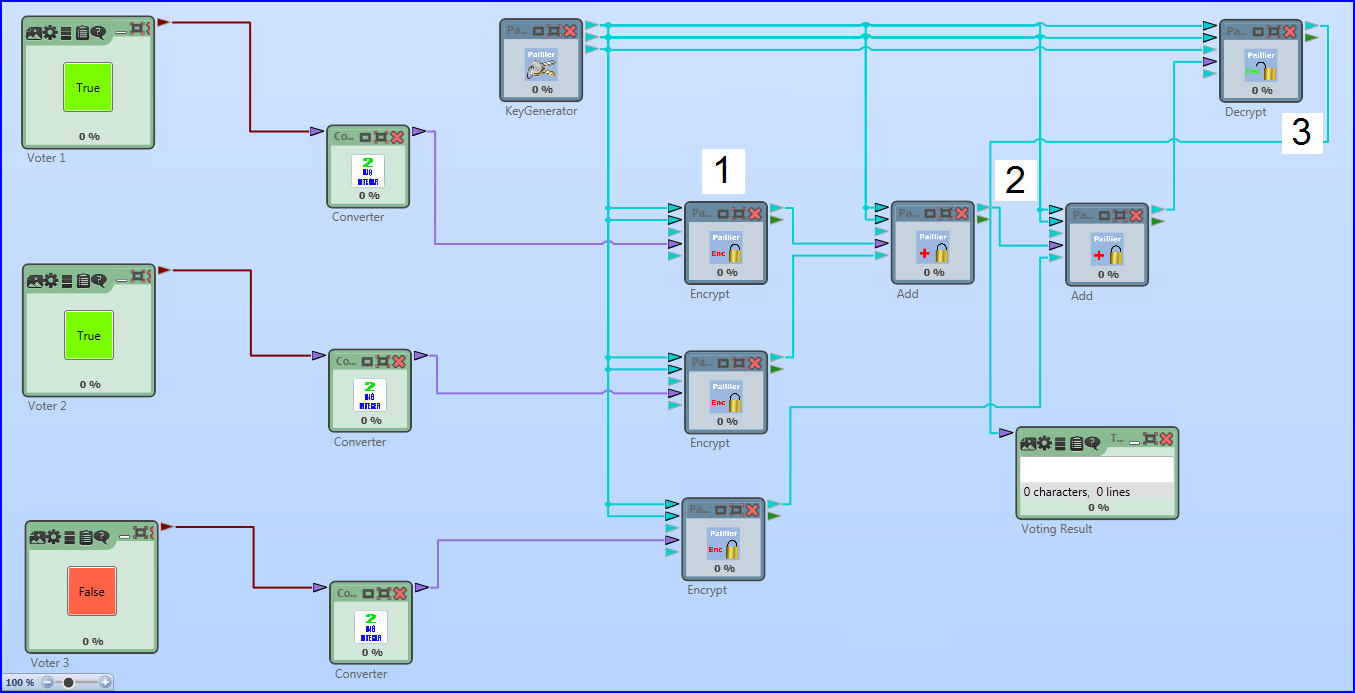
\includegraphics[scale=0.4]{figures/CT2-PaillierVoting.png}
\caption{Voting-Beispiel f�r Paillier} 
\label{CT2-PaillierVoting}
\end{center}
\end{figure}

\item Ein weiteres Anwendungsgebiet f�r homomorphe Chiffren ist \glqq Secure Multiparty Computation\grqq. Hierbei berechnen mehrere Parteien gemeinsam eine vorgegebene Funktion. Jede der Parteien steuert einen Input f�r die zu berechnende Funktion bei. Das Ziel der Berechnung ist es, alle Inputs und auch die Zwischenergebnisse geheim zu halten, w�hrend nur das Ergebnis der Funktion bekannt wird. Die Verwendung homomorpher Chiffren hilft dabei, diese Berechnungen auf verschl�sselten Daten durchzuf�hren. Da sich allerdings unter der homomorphen Chiffre von Paillier nur Additionen (und z.B. keine Multiplikationen durchf�hren lassen), m�ssen noch weitere geeignete Methoden verwendet werden. Einen guten Einstieg in dieses Thema bietet Wikipedia \cite{Wiki_SMC}.

\item Weiterhin wird erwartet, dass homomorphe Chiffren im Bereich Cloud Computing enorme Vorteile bringen k�nnen. Mittels sogenannter voll-homomorpher Kryptosysteme \cite{Wiki_HomEnc} wird es m�glich sein, komplette Anwendungen auf verschl�sselten Daten durchzuf�hren. Hierzu ist es notwendig, dass unter der homomorphen Verschl�sselung die beiden Operationen Addition und Multiplikation durchgef�hrt werden k�nnen (im Gegensatz zum Paillier-Kryptosystem, welches nur die Addition unterst�tzt). Ein solches Kryptosystem wurde erstmals 2009 von Craig Gentry vorgestellt \cite{Gentry2009}.
\end{enumerate}

% -----------------------------------------------------------------------------
\section{Homomorphe Chiffren in CrypTool}

\subsection{CrypTool~2}
In CrypTool~2\index{CT2} findet man bereits eine Implementierung des Paillier-Kryptosystems (siehe Bild \ref{CT2-Paillier}). Unter den fertigen Vorlagen finden sich Methoden zur Erzeugung der kryptographischen Schl�ssel (Paillier Key Generator), ein Beispiel f�r eine Ver- und Entschl�sselung mittels Paillier (Paillier Text), sowie Beispiele, die die homomorphen Eigenschaften von Paillier aufzeigen (Paillier Addition, Paillier Blinding und Paillier Voting).

\begin{figure}[ht]
\begin{center}
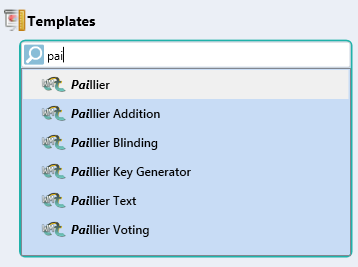
\includegraphics[scale=0.8]{figures/CT2-Paillier.png}
\caption{Paillier-Kryptosystem in CrypTool~2 (CT2)} 
\label{CT2-Paillier}
\end{center}
\end{figure}

\newpage

\subsection{JCrypTool}

Im JCrypTool\index{JCT} gibt es eine Implementierung (siehe Bild \ref{JCT-HomEnc}), die die homomorphen Eigenschaften verschiedener Kryptosysteme visualisiert. F�r RSA und Paillier wird gezeigt, dass jeweils Multiplikationen (f�r RSA) und Additionen (f�r Paillier) auf verschl�sselten Werten m�glich sind. F�r das voll-homomorphe Kryptosystem von Gentry k�nnen sowohl Multiplikationen als auch Additionen auf verschl�sselten Werten durchgef�hrt werden.

\begin{figure}[ht]
\begin{center}
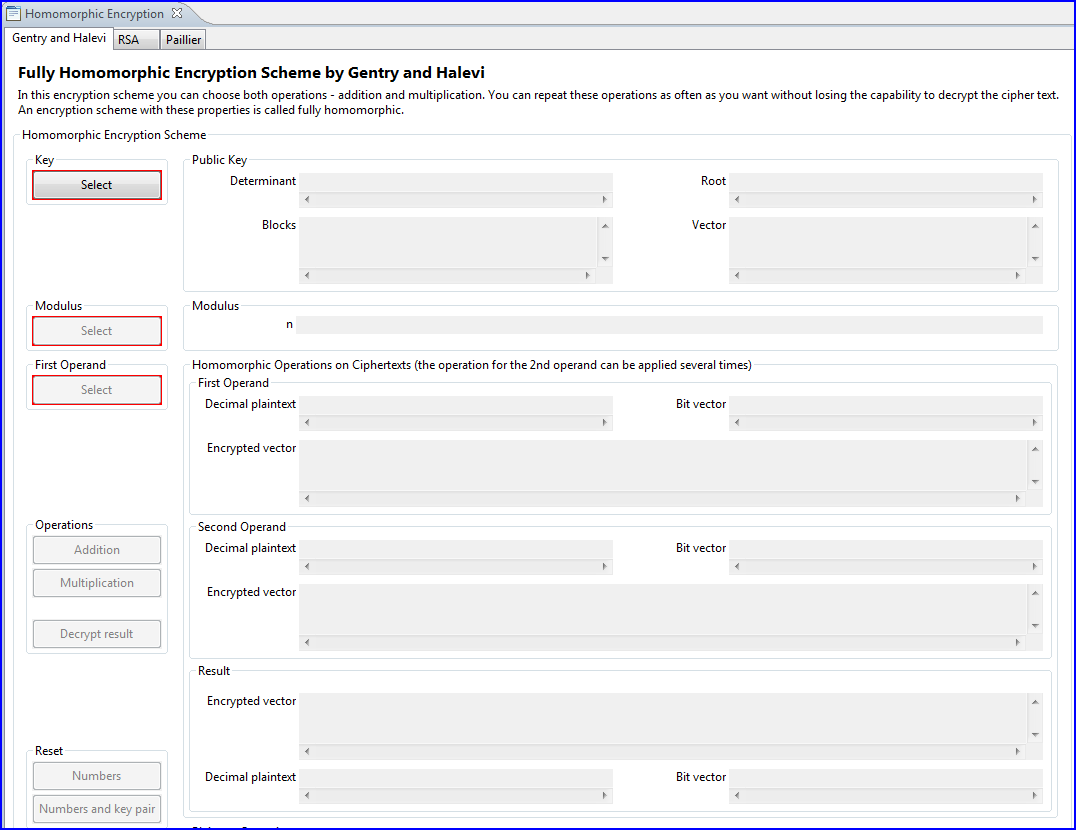
\includegraphics[scale=0.4]{figures/JCT-HomEnc.PNG}
\caption{Kryptosysteme mit homomorphen Eigenschaften in JCrypTool (JCT)} 
\label{JCT-HomEnc}
\end{center}
\end{figure}



%------------------------------------------------------------------------------
\putbib[../de/references]
\addcontentsline{toc}{section}{Literaturverzeichnis}
\end{bibunit}

\noindent Alle Links im Artikel wurden am 15.07.2016 �berpr�ft.


% Local Variables:
% TeX-master: "../script-de.tex"
% End:



\renewcommand{\CTBChapName}{(Chap DLogFact)}      % $Id:
% !Mode:: "TeX:DE"    % Setting document mode and submode for WinEdt
% ..............................................................................
% Studie aktuelle akademische Resultate für das Lösen diskreter Logarithmen und zur Faktorisierung
% ~~~~~~~~~~~~~~~~~~~~~~~~~~~~~~~~~~~~~~~~~~~~~~~~~~~~~~~~~~~~~~~~~~~~~~~~~~~~~~
% be_2016-07-14: Housekeeping: " \\\" --> "\\" done (d+E).

\begin{refsegment}




\newcommand{\mmod}{\hspace{1mm}{\rm mod}\hspace{1mm}}
\newcommand{\lf}{\left\lfloor}
\newcommand{\rf}{\right\rfloor}
\newcommand{\norm}{|\!|}


\newcommand{\phin}{\phi(N)}
\newcommand{\bigO}{{\cal O}}
\newcommand{\res}{\textrm{res}}
\newcommand{\poly}{\textrm{poly}}
\newcommand{\dlog}{\textrm{dlog}}
%16xxxxxxxxxxxxxx\newcommand{\bi}{\begin{itemize}}
%16xxxxxxxxxxxxxx\newcommand{\ei}{\end{itemize}}
\newbox\BeweisSym
\setbox\BeweisSym=\hbox{%
\unitlength=0.18ex%
\begin{picture}(10,10)
\put(0,0){\framebox(9,9){}}
\put(0,3){\framebox(6,6){}}
\end{picture}}

%%16 Folgendes nicht verewendet (Warum war es mal mit Punkt und Blank, und mal mit Doppelpunkt am Ende?)
%\newenvironment{Proof}{\noindent{\bf Beweis:}$\mbox{}\;$}%
%{\hfill\copy\BeweisSym\linebreak\par\noindent}
%\renewenvironment{proof}{\noindent{\it Beweis. }$\mbox{}\;$}
%{\par\noindent}
%\newtheorem{Claim}{Claim}

\newtheorem{defi}{Definition}
\newtheorem{theo}[defi]{Theorem}
\newtheorem{coro}[defi]{Corollary}
\newtheorem{assu}[defi]{Assumption}
\newtheorem{lemm}[defi]{Lemma}
\newtheorem{prop}[defi]{Proposition}
\newtheorem{nota}[defi]{Notation}
\newtheorem{rema}[defi]{Remark}
\newtheorem{fact}[defi]{Fact}


%--------------------------------------------------------------------
\newpage
\hypertarget{Chapter_Dlog-FactoringDead}{}
\chapter%[Resultate zur Widerstandskraft diskreter Logarithmen und zur Faktorisierung]
{Studie über aktuelle akademische Resultate für das Lösen diskreter Logarithmen und zur Faktorisierung -- und wie man in der Praxis reagiert}
\chaptermark{Widerstandskraft diskreter Logarithmen}
%
%% \chapter[\texorpdfstring{Studie über aktuelle akademische Resultate für das Lösen diskreter\\ Logarithmen und zur Faktorisierung}{Studie über aktuelle akademische Resultate für das Lösen diskreter Logarithmen und zur Faktorisierung}]{Studie über aktuelle akademische Resultate für das Lösen diskreter Logarithmen und zur Faktorisierung -- und wie man in der Praxis reagiert}% So alles wie gewollt, und auch keine hyperref-Warnung wegen des\\.
                 % \texorpdfstring{X}{Y}  X bekommt man per nameref und steht im normalen Inhaltsverzeichnis;
                 %                        Y steht im Inhaltsverzeichnis links beim Scrollen.
%
%   Ziel war, den längeren Text nur in die Kapitelüberschrift, nicht ins Inhaltsverzeichnis zu bringen, UND
%           nur im Inhaltsverzeichnis-String einen Zeilenumbruch zu erzwingen.
%   \chapter[Studie über aktuelle akademische Resultate für das Lösen diskreter\\ Logarithmen und zur Faktorisierung]{Studie über aktuelle akademische Resultate für das Lösen diskreter Logarithmen und zur Faktorisierung -- und wie man in der Praxis reagiert}% So alles wie gewollt, aber hyperref-Warnung wegen des\\.
% * \chapter[ALTERNATIV für Inhaltsverzeichnis]{ÜBERSCHRIFT}
% * \chapter*{ÜBERSCHRIFT}  (so kein Eintrag ins Inhaltsverzeichnis)
% * \chapter[<short title>]{<title>}
% * https://de.sharelatex.com/learn/Sections_and_chapters
% * \texorpdfstring{<tex>}{<PDF>}
% * \texorpdfstring{Code im Text}{Code für bookmark}
% * Bsp.: \section{  \texorpdfstring{CO\textsubscript{2}} {CO\string_(2)}  }
% * Siehe: http://de.comp.text.tex.narkive.com/3cPmE95e/benutzung-von-texorpdfstring
% * ABER: Nun bei Verwendung von \nameref immer der Umbruch drin und ich schaffte nicht, den wieder rauszubringen.
% * (siehe introduction.tex, Ende von Vorwort, S. xvi)
\label{Chapter_Dlog-FactoringDead}
\index{Logarithmusproblem!diskret}\index{Faktorisierung}

(\hyperlink{author_Antoine-Joux}{Antoine Joux}, \hyperlink{author_Arjen-Lenstra}{Arjen Lenstra} \& \hyperlink{author_Alexander-May}{Alexander May}; April 2014)\\

\noindent (Übersetzung ins Deutsche: Patricia Wienen, 2016)\\
% Übersetzung:
% - 'smooth co-factor'  glatter Cofaktor
% - 'Hensel lifting process'   Hensel Lifting bzw. Hensel Lift Prozess
% - 'multiple dlogs'   viele dlogs
% - 'description length'   Beschreibungslänge
% - 'for discrete log-based ?'     'für Dlog-basierte Verfahren ?'



\noindent {\bf Abstract:}
Neuste algorithmische Entwicklungen für das Lösen diskreter Logarithmen in endlichen
Körpern mit kleiner Charakteristik führten zu einer gewissen (publizistisch beförderten)
Unsicherheit bei kryptographischen Nutzern bezüglich des Einflusses auf die Sicherheit kürzlich entwickelter Kryptoverfahren (siehe dazu beispielsweise die Diskussion in~\cite{Blackhat2013} unter dem Stichwort~\glqq Cryptocalypse\grqq).\index{Cryptocalypse}   Dieses Kapitel gibt einen Überblick über die zur Zeit besten Algorithmen für das Berechnen diskreter Logarithmen in verschiedenen Gruppen und über den Status des Faktorisierungsproblems. Unser Ziel ist zu klären, was im Moment algorithmisch machbar ist und wofür erst weitere bedeutende Durchbrüche nötig sind. Zusammenfassend sehen wir im Moment keinen Weg, wie man die bestehenden algorithmischen Prozesse für endliche Körper mit kleiner Charakteristik entweder auf Körper mit großer Charakteristik oder auf das ganzzahlige Faktorisierungsproblem erweitern könnte.
% Our analysis leads to practical mid- and long-term suggestions both for the deployed cryptographic systems and for the choice of their key sizes.


%%%%%
\newpage
% So ist wohl der schwarze Punkt in Inhaltsverzeichnis behoben, aber da \\ ein TeX-Kommando ist,
% hat man die Warnung: Package hyperref Warning: Token not allowed in a PDF string (PDFDocEncoding): removing\\
% \section[Generische Algorithmen für das diskrete Logarithmus-Problem in beliebigen\\
%         Gruppen]
%        {Generische Algorithmen für das diskrete Logarithmus-Problem in beliebigen Gruppen}
%\section{\texorpdfstring{Generische Algorithmen für das diskrete Logarithmus-Problem in beliebigen\\
%         Gruppen}
%	 {Generische Algorithmen für das diskrete Logarithmus-Problem in beliebigen Gruppen}
%	}
% - texorpdfstring{...}{...} hat 2 Argumente: Das 2. ist für die Bookmarks?
%   Real war es so: Nicht klar, wo 0x stand; 1x stand Inhaltsverzeichnis links und im Inhaltsverzeichnis im Text
%                   selbst; 3x stand stand im Kapitel als Überschrift. Durch die Abkürzung Dlog waren die ganzen
%                   Black boxes verschwunden -- aber bei Gelegenheit mal untersuchen ! TodoTodo.
%  \section[0xGenerische Algorithmen für das Dlog\--Pro\-b\-lem in beliebigen Gruppen]
%          {\texorpdfstring{1xGenerische Algorithmen für das Dlog\--Pro\-b\-lem in beliebigen Gruppen}
%  	                   {2xGenerische Algorithmen für das Dlog-Problem in beliebigen Gruppen}
%  	   }
\section{Generische Algorithmen für das Dlog-Problem in beliebigen Gruppen}
\label{generic}

{\bf Management Summary: Die Widerstandsfähigkeit des diskreten Logarithmus-Pro\-b\-lems
hängt von der Gruppe ab, über die es definiert ist. In diesem Kapitel betrachten wir kryptoanalytische Algorithmen, die für beliebige Gruppen funktionieren. Aus kryptographischem Blickwinkel ist es erstrebenswert, solche Gruppen zu identifizieren, für die sich keine besseren Algorithmen finden lassen. Ein Kandidat dafür sind Gruppen über Elliptischen Kurven.\\[0.1cm]}

In diesem Kapitel beschreiben wir {\em allgemeine} kryptoanalytische Algorithmen, die sich auf {\em jede} endliche abelsche Gruppe anwenden lassen. Das heißt, jede in der Kryptographie verwendete Gruppe -- z. B. multiplikative Gruppen über endlichen Körpern oder über Elliptischen Kurven -- ist für diese Algorithmen anfällig. Wir werden sehen, dass wir mit der Pollard-Rho-Methode in einer Gruppe der Ordnung $n$ immer einen diskreten Logarithmus in $\bigO(\sqrt n)$ Schritten berechnen können. Umgekehrt bedeutet das, dass man eine Gruppe mit einer Ordnung von mindestens $2^{2k}$ wählen muss, um ein Sicherheitslevel von $2^{k}$ zu erreichen. Z.B. muss man für ein Sicherheitslevel von $80$ Bits eine Gruppe der Ordnung $160$ Bits oder mehr wählen. Das erklärt, warum wir in der Praxis üblicherweise Gruppen über Elliptischen Kurven mit einer Ordnung von mindestens $160$ Bits wählen.

Des Weiteren sei $G$ eine Gruppe der Ordnung $n$ und sei $n=p_1^{e_1} \cdot \ldots \cdot p_{\ell}^{e_{\ell}}$ die Primfaktorzerlegung von $n$. Wir werden sehen, dass diskrete Logarithmen in $G$ in Zeit $\bigO(e_1 \sqrt{p_1} + \ldots + e_{\ell}\sqrt{p_{\ell}})$ berechnet werden können. Man bemerke, dass diese Beschränkung äquivalent ist zu Pollard's Beschränkung $O(\sqrt n)$ g.d.w. $n$ prim ist. Andernfalls wird die Komplexität der Berechnung des diskreten Logarithmus hauptsächlich beschränkt durch die Größe des größten Primteilers der Gruppenordnung. Dies erklärt, warum z.B. Schnorr-/DSA-Signaturen in Gruppen implementiert werden, die per Konstruktion einen Primfaktor von mindestens $160$ Bit Länge enthalten. Das erklärt außerdem, warum Gruppen über Elliptischen Kurven üblicherweise primer Ordnung sind oder deren Ordnung nur einen sehr kleinen \textbf{glatten Cofaktor} enthält.

%\DIFaddbegin \DIFadd{\fbox{It should be $\bigO(\sqrt{p_1} + \ldots + \sqrt{p_{\ell}}) \leq \bigO \left( \left(\sum_ {i=1}^\ell e_i  \right)\max_{i}(\sqrt p_i) \right)$}
%}


\DIFaddend \subsection{Die Pollard-Rho-Methode}
\index{Pollard-Rho}
Sei $G$ eine endliche abelsche Gruppe. Sei $g$ ein Generator einer großen Untergruppe $G' = \{g, g^2, \ldots, g^n\} \subseteq G$ (z.B. könnte $g$ die Gruppe $G$ selbst generieren). Sei $y=g^{x}$. Dann beschreibt das diskrete Logarithmus-Problem den Versuch, bei Eingabe von $g$ und $y$ den Wert $x \mod n$ auszugeben.
Wir schreiben $x=\dlog_g(y)$.

Die Pollard-Rho-Methode versucht, Elemente $g^{a_i}y^{b_i} \in G'$ mit $a_i, b_i \in \mathbb{N}$ in einer pseudozufälligen, aber deterministischen Art und Weise zu erzeugen. Der Einfachheit halber nehmen wir an, dass wir zufällige Elemente von den $n$ Elementen in $G'$ erzeugen. Dann erwarten wir wegen des Geburtstagsparadoxons nach höchstens $\bigO(\sqrt n)$ Schritten zwei identische Elemente zu erhalten. In unserem Fall bedeutet das
$$
  g^{a_i}y^{b_i} = g^{a_j}y^{b_j}.
$$
Dies kann umgeschrieben werden als $g^{\frac{a_i-a_j}{b_j-b_i}} = y$. Daraus wiederum folgt, dass wir unseren diskreten Logarithmus aus $x \equiv \frac{a_i-a_j}{b_j-b_i} \mmod n$ erhalten können.

Somit kann man mit der Pollard-Rho-Methode den diskreten Logarithmus in jeder endlichen abelschen Gruppe der Ordnung $n$ in $\bigO(\sqrt n)$ Schritten berechnen. Durch die Nutzung von Techniken zum Auffinden von Schleifen (sogenannter cycle-finding techniques) kann man außerdem zeigen, dass die Pollard-Rho-Methode mit konstantem Speicherbedarf implementiert werden kann.

Außerdem ist es auch möglich, die Effizienz von Quadratwurzel-Algorithmen zu verbessern, wenn mehrere diskrete Logarithmen in derselben Gruppe erwünscht sind: Bei der Berechnung von $L$ verschiedenen Logarithmen kann man die globalen Kosten von $\bigO (L\sqrt{n})$ auf $\bigO (\sqrt{Ln})$ reduzieren~\cite{multiple2014}.


\subsection{Der Silver-Pohlig-Hellman-Algorithmus}
\index{Silver-Pohlig-Hellman}
Wie zuvor sei $y = g^{x}$ für einen Generator $g$ der Ordnung $n$. Wir wollen den diskreten Logarithmus $x \mmod n$ berechnen. Außerdem sei $n=p_1^{e_1} \cdot \ldots \cdot p_{\ell}^{e_{\ell}}$ die Primfaktorzerlegung von $n$. Dann gilt nach dem Chinesischen Restsatz, dass $x \mmod n$ eindeutig definiert wird durch folgendes System von Kongruenzen:
\begin{equation}
\label{crt}
\begin{array}{lll}
  x & \equiv & x_1 \mmod p_1^{e_1}\\
    & \vdots\\
  x & \equiv & x_{\ell} \mmod p_{\ell}^{e_{\ell}}.	
\end{array}
\end{equation}

Der Algorithmus von Silver-Pohlig-Hellman berechnet alle diskreten Logarithmen $x_i \mmod p_i$ in den Untergruppen mit den Ordnungen $p_i$ in $\bigO(\sqrt{p_i})$ Schritten durch Verwendung der Pollard-Rho-Methode. Danach ist es relativ einfach einen Logarithmus modulo der Primzahlpotenz $x_i \mmod p_i^{e_i}$ mittels eines \textbf{Hensel-Lift-Prozesses} zu finden, der $e_i$ Aufrufe an die diskrete Logarithmus-Prozedur modulo $p_i$ ausführt. In einem \textbf{Hensel-Lift-Prozess} starten wir mit einer Lösung $x_i \mmod p_i$ und berechnen dann nacheinander $x_i \mmod p_i^2$, $x_i \mmod p_i^3$ usw. bis zu $x_i \mmod p_i^{e_i}$ (siehe~\cite{May2013} für Hensels Schema).

Schlussendlich berechnet man den gewünschten diskreten Logarithmus $x \mmod n$ aus dem obigen System von Gleichungen~(\ref{crt}) über den Chinesischen Restsatz.
Insgesamt wird die Laufzeit hauptsächlich festgelegt durch die Berechnung von $x_i \mmod p_i$ für den größten Primfaktor $p_i$. Damit ist die Laufzeit ungefähr $\bigO(\max_i\{\sqrt p_i\})$.


\subsection{Wie man Laufzeiten misst}
Im Verlauf dieser Studie wollen wir die Laufzeit von Analyse-Algorithmen für diskrete Logarithmen abschätzen als Funktion der Bitgröße $n$. Es gilt, dass jede Ganzzahl $n$ mit (ungefähr) $\log n$ Bits geschrieben werden kann, wobei der Logarithmus zur Basis $2$ gewählt wird. Die {\em Bitgröße} von $n$ ist damit $\log n$.

Um unsere Laufzeiten auszudrücken nutzen wir die Notation $L_n[b,c]=\exp^{c \cdot (\ln n)^{b}(\ln\ln n)^{1-b}}$ für Konstanten $b \in [0,1]$ und $c>0$. Bemerke, dass $L_n[1,c]=e^{c \cdot \ln n} = n^c$ eine Funktion ist, die für konstantes $c$ polynomiell in $n$ ist. Deshalb sagen wir, dass $L_n[1,c]$ {\em polynomiell} in $n$ ist. Bemerke außerdem, dass $L_n[1,c]=n^c = (2^{c})^{\log_2 n}$ eine in $\log n$ exponentielle Funktion ist. Deshalb sagen wir, dass $L_n[1,c]$ {\em exponentiell} in der Bitgröße $\log n$ von $n$ ist. Damit erreicht unser Pollard-Rho-Algorithmus eine erwartete Laufzeit von $L[1,\frac 1 2]$.

Auf der anderen Seite ist $L_n[0,c] = e^{c \cdot \ln\ln n} = (\ln n)^c$ {\em polynomiell} in der Bitgröße von $n$. Merke, dass der erste Parameter $b$ für die Laufzeit wichtiger ist als der zweite Parameter $c$, da $b$ zwischen polynomieller und exponentieller Laufzeit interpoliert. Als Kurzschreibweise definieren wir $L_n[b]$, wenn wir die Konstante $c$ nicht spezifizieren wollen.

Einige der wichtigsten Algorithmen, die wir in den nachfolgenden Kapitels besprechen, erreichen eine Laufzeit von $L_n[\frac 1 2 +o(1)]$ oder $L_n[\frac 1 3 +o(1)]$ (wobei das $o(1)$ für $n\to\infty$ verschwindet), welche eine Funktion ist die schneller wächst als jedes Polynom, aber langsamer als exponentiell. Für kryptographische Verfahren sind solche Angriffe völlig akzeptabel, da das gewünschte Sicherheitslevel einfach erreicht werden kann durch moderates Anpassen der Schlüsselgrößen.

Der aktuelle Algorithmus von Joux et al. für die Berechnung diskreter Logarithmen in endlichen Körpern mit kleiner Charakteristik erreicht jedoch eine Laufzeit von $L_n[o(1)]$, wobei $o(1)$ gegen $0$ geht für $n \to \infty$. Das bedeutet, dass diese Algorithmen in quasi-polynomieller Zeit laufen, und dass die zugrunde liegenden Körper nicht länger akzeptabel sind für kryptographische Anwendungen. Ein endlicher Körper $\mathbb{F}_{p^n}$ hat eine kleine Charakteristik, wenn $p$ klein ist, d.h. der Basiskörper (base field) $\mathbb{F}_p$ ist klein und der Grad $n$ der Körpererweiterung ist üblicherweise groß. In den aktuellen Algorithmen brauchen wir ein kleines $p$, da diese Algorithmen über alle $p$ Elemente im Basiskörper $\mathbb{F}_p$ laufen.


\subsection{Unsicherheit durch Quantencomputern}
\index{Quantencomputer}
In 1995 veröffentlichte Shor einen Algorithmus für die Berechnung diskreter Logarithmen und Faktorisierungen auf einem Quantencomputer. Er zeigte, dass die Berechnung diskreter Logarithmen in {\em jeder} Gruppe der Ordnung $n$ in polynomieller Zeit durchgeführt werden kann, die fast $\bigO(\log n^2)$ entspricht. Dieselbe Laufzeit gilt für die Berechnung der Faktorisierung einer Ganzzahl $n$. Diese Laufzeit ist nicht nur polynomiell, die Angriffe sind sogar noch effizienter als die kryptographischen Verfahren selbst! Das wiederum bedeutet, dass das Problem nicht durch bloßes Anpassen der Schlüsselgrößen behoben werden kann.

Sollten wir also in den nächsten Jahrzehnten die Entwicklung groß angelegter Quantencomputer miterleben, muss folglich die ganze klassische, auf Dlog oder Faktorisierung basierende Kryptographie ersetzt werden. Man sollte allerdings betonen, dass die Konstruktion großer Quantencomputer mit vielen Qubits sehr viel schwieriger zu sein scheint als die seines klassischen Gegenstücks, da die meisten kleinen Quantensysteme nicht gut skalieren und ein Problem mit Dekohärenz haben.\\[0.1cm]

\noindent {\bf Empfehlung:} Es scheint schwierig zu sein, die Entwicklungen in der Konstruktion von Quantencomputern vorherzusagen. Experten der Quantenphysik sehen aber derzeit keine unüberwindbaren Hindernisse, die die Entwicklung großer Quantencomputer auf lange Sicht behindern würden. Es dürfte sehr wichtig sein, den aktuellen Fortschritt in diesem Gebiet im Blick zu behalten und in den nächsten 15 Jahren alternative quanten-resistente Kryptoverfahren zur Hand zu haben.\\[0.1cm]

\noindent {\bf Referenzen und weiterführende Literatur:}
Wir empfehlen die Bücher von Menezes, van Oorschot und Vanstone~\cite{Menezes2001}, Joux~\cite{Joux2009} und Galbraith~\cite{Galbraith2012} zur Studie kryptoanalytischer Techniken. Einen einführenden Kurs in Kryptoanalyse stellt Mays Vorlesungsskript zur Kryptoanalyse zur Verfügung~\cite{May2012a,May2012b}. Eine Einleitung zu Quantenalgorithmen findet sich in den Büchern von Homeister~\cite{Homeister2007} und Mermin~\cite{Mermin2008}.

Die Algorithmen in diesem Kapitel wurden ursprünglich in den hervorragenden Arbeiten von Pollard~\cite{Pollard1975,Pollard2000} und Shor~\cite{Shor1994} vorgestellt.
Generische Algorithmen für viele Dlogs wurden kürzlich untersucht in~\cite{multiple2014}.


%%%%%
\newpage
%\section{\texorpdfstring{Beste Algorithmen für Primkörper $\mathbb{F}_p$}{Beste Algorithmen für Primkörper Fp}}
\section{\texorpdfstring{Beste Algorithmen für Primkörper $\mathbb{F}_p$}{Beste Algorithmen für Primkörper Fp}}
\label{prime_field}
\index{Primkörper}
{\bf Management Summary: Primkörper $\mathbb{F}_p$ sind -- neben Elliptischen Kurven -- die Standardgruppe für das diskrete Logarithmus-Problem. In den letzten 20 Jahren gab es für diese Gruppen keinen signifikanten algorithmischen Fortschritt. Sie sind immer noch eine gute Wahl für Kryptographie.\\[0.1cm]}

In Kapitel~\ref{generic} haben wir gelernt, dass wir in jeder endlichen abelschen Gruppe der Ordnung $n$ den diskreten Logarithmus in $\bigO(\sqrt n)$ Schritten bestimmen können. Merke, dass sowohl die Pollard-Rho-Methode als auch der Silver-Pohlig-Hellman-Algorithmus aus Kapitel~\ref{generic} keine andere Eigenschaften der {\em Repräsentation} von Gruppenelementen nutzen als ihre Eindeutigkeit. In diesen Methoden werden Gruppenelemente einfach durch Gruppenoperationen und Test auf Gleichheit von Elementen berechnet. Algorithmen dieser Art werden in der Literatur als {\em generisch} bezeichnet.

Es ist bekannt, dass generische Algorithmen diskrete Logarithmen nicht in besserer Zeit als der Silver-Pohlig-Hellman-Algorithmus~\cite{Shoup1997} berechnen können. Damit können die Algorithmen aus Kapitel~\ref{generic} als optimal betrachtet werden, wenn keine weitere Information über die Gruppenelemente bekannt ist.

Wenn wir unsere Gruppe $G$ spezifizieren als die multiplikative Gruppe über den endlichen Körper $\mathbb{F}_p$ mit $p$ prim, können wir sogar die Repräsentation der Gruppenelemente ausnutzen. Natürliche Repräsentanten von $\mathbb{F}_p$ sind die Ganzzahlen $0, \ldots, p-1$. Damit können wir z.B. die Primfaktorzerlegung dieser Ganzzahlen verwenden. Dies wird gemacht in den Algorithmen des sogenannten Typs {\em Index-Calculus} für diskrete Logarithmen. Dieser Typ von Algorithmen bildet derzeit die Klasse mit den besten Laufzeiten für diskrete Logarithmen über Primkörper, prime Körpererweiterungen (Kapitel~\ref{ffs}) und für das Faktorisierungsproblem (Kapitel~\ref{factor}).

Wir werden jetzt einen Index-Calculus-Algorithmus an Hand eines sehr einfachen Beispiels veranschaulichen.


%%%%%
\subsection{Eine Einleitung zu Index-Calculus-Algorithmen}
\label{simple}
\index{Index-Calculus}
Ein Index-Calculus-Algorithmus besteht aus drei grundlegenden Schritten.

\begin{description}
\item[Faktorbasis:] Definition der Faktorbasis $F=\{f_1, \ldots, f_k\}$. Wir wollen die Gruppenelemente ausdrücken als Potenzen von Elementen der Faktorbasis.

\item[Relationen finden:] Finde Elemente $z_i:=g^{x_i} \in G$ für eine ganze Zahl $x_i$, die mit der Faktorbasis bestimmt werden können. Das bedeutet
$$
  g^{x_i} = \prod_{j=1}^k f_j^{e_{ij}}.
$$
Schreiben wir diese Gleichung zur Basis $g$ erhalten wir eine {\em Relation}
$$
  x_i \equiv \sum_{j=1}^k e_{ij}\textrm{dlog}_g(f_j) \mmod n,
$$
wobei $n$ die Ordnung von $g$ ist. Dies ist eine lineare Gleichung in den $k$ Unbekannten $\textrm{dlog}_g(f_1), \ldots, \textrm{dlog}_g(f_k)$. Sobald wir $k$ linear unabhängige Relationen dieses Typs haben, können wir die Unbekannten mit Linearer Algebra berechnen. Das bedeutet, dass wir erst alle diskreten Logarithmen der Faktorbasis berechnen müssen, bevor wir den gewünschten individuellen Logarithmus von $y$ bestimmen.

\item[Dlog-Berechnung:] Drücke $yg^r = g^{x+r} = \prod_{j=1}^k f_j^{e_j}$ in der Faktorbasis für eine ganze Zahl~$r$ aus.
Das gibt uns eine neue Relation
$$
  x+r \equiv \sum_{j=1}^k e_{j}\textrm{dlog}_g(f_j) \mmod n,
$$
die in der einzigen Unbekannten $x=\textrm{dlog}_g y$ einfach gelöst werden kann.
\end{description}

Lassen Sie uns ein einfaches Beispiel für einen Index-Calculus-Algorithmus geben, das $x=\textrm{dlog}_2(5)$ in $\mathbb{F}_{11}^*$ berechnet. Da $2$ die multiplikative Gruppe $\mathbb{F}_{11}^*$ generiert, ist $2$ von der Ordnung $10$.

\begin{description}
\item[Faktorbasis:] Definiere $F=\{-1,2\}$.

\item[Relationen finden:] $2^1 = (-1)^0 2^1$ gibt uns eine erste triviale Relation
$$
  1 \equiv 0 \cdot \textrm{dlog}_2(-1) + 1\cdot \dlog_2(2) \mmod 10.
$$
Wenn wir $2^6 = 64 \equiv -2 \mmod 11$ berechnen, erhalten wir eine zweite Relation
$$
  6 \equiv 1\cdot \dlog_2(-1) + 1 \cdot \dlog_2(2) \mmod 10.
$$
Damit können wir das System von linearen Gleichungen lösen:
$$
\left(
\begin{array}{ll}
0 & 1\\
1 & 1
\end{array}
\right)
\cdot
\left(
\begin{array}{l}
\dlog_2(-1)\\
\dlog_2(2)
\end{array}
\right)
%
\equiv
%
\left(
\begin{array}{l}
1\\
6
\end{array}
\right) \mmod 10.
$$
Als eindeutige Lösung erhalten wir $\dlog_2(-1) \equiv 5$ und $\dlog_2(2) \equiv 1$.

\item[Dlog-Berechnung:] Wegen $5 \cdot 2^{1} = 10 \equiv -1 \mmod 11$ erhalten wir
$$
  x + 1 \equiv 1 \cdot \dlog(-1) + 0 \cdot \dlog(2) \mmod 10.
$$
Dies führt zu der Lösung $x \equiv 4 \mmod 10$.
\end{description}

\noindent {\bf Laufzeit:}
Eine große Faktorbasis zu wählen macht es einfacher, Relationen zu finden, da es die Wahrscheinlichkeit erhöht, dass sich eine bestimmte Zahl in der Faktorbasis aufteilt. Auf der anderen Seite müssen wir für eine große Faktorbasis mehr Relationen finden, um die Dlogs aller Faktorbasiselemente zu berechnen. Eine Optimierung dieses Kompromisses führt zu einer Laufzeit von $L_p[\frac 1 2]$ für den "`relation finding"'-Schritt und ebenfalls $L_p[\frac 1 2]$ für die Berechnung des individuellen diskreten Logarithmus in Schritt~3.

Lasst uns kurz die Vor- und Nachteile des obigen, simplen Index-Calculus-Algorithmus aus der Sicht eines Kryptoanalysten diskutieren.

\noindent {\bf Vorteile:}
\begin{itemize}
\item Für $g^{x_i} = \prod_{j=1}^k f_j^{e_{ij}}$ ist es trivial, den diskreten Logarithmus auf der linken Seite zu berechnen.
\end{itemize}

\noindent {\bf Nachteile:}
\begin{itemize}
\item Wir müssen relativ große Zahlen $g^{x_i}$ über die ganzen Zahlen mit einbeziehen. Man kann zeigen, dass dies zwangsläufig zu einer Laufzeit von $L_p[\frac 1 2]$ führt, und dass es keine Hoffnung gibt, unter die Konstante $\frac 1 2$ zu kommen.
\DIFdelbegin %DIFDELCMD <

\DIFdelend \item Wir müssen alle diskreten Logarithmen für die Faktorbasiselemente berechnen. Dies ist allen Index-Calculus-Algorithmen zu eigen.
\end{itemize}

Wir werden den ersten Nachteil eliminieren, indem wir Faktorisierung über Zahlkörpern erlauben.
Der zweite Nachteil wird eliminiert, indem man eine Faktorbasis wählt, bei der man die Dlogs ihrer Elemente sehr effizient berechnen kann.
%Let us illustrate our Index Calculus in a (trivial) commuting diagram.



\subsection[Das Zahlkörpersieb zur Berechnung des Dlog]{Das Zahlkörpersieb zur Berechnung des Dlog\footnotemark}
\footnotetext{%
   Beim Zahlkörpersieb zur Berechnung des Dlog gibt es -- im Gegensatz zum Zahlkörpersieb
   zur Faktorisierung in Abschnitt~\ref{nfs-factor} -- nur {\bf das} Zahlkörpersieb.
   Die Unterscheidung Special versus General fällt hier weg.}
\label{nfs-dlog}
\index{Zahlkörpersieb}

Ein Zahlkörper $\mathbb{Q}[\alpha]$ ist ein $k$-dimensionaler Vektorraum über $\mathbb{Q}$ und kann erzeugt werden durch Anfügen einer Nullstelle $\alpha$ eines irreduziblen Polynoms $f$ vom Grad $k$ an $\mathbb{Q}$. Das bedeutet, wir können jedes Element von $\mathbb{Q}[\alpha]$ schreiben als $a_0+a_1\alpha + \ldots a_{k-1}\alpha^{k-1}$ mit $a_i \in \mathbb{Q}$. Wenn wir die $a_i$ auf die ganzen Zahlen beschränken, befinden wir uns im Ring $\mathbb{Z}[\alpha]$.

Das Zahlkörpersieb ist ebenfalls ein Index-Calculus-Algorithmus. Verglichen
mit dem vorigen Ansatz hat er den Vorteil, kleinere Zahlen zu verwenden.
Das wird erreicht durch die Wahl einer spezifischen Repräsentation des
Primkörpers $\mathbb{F}_p$, der implizit definiert ist als endlicher Körper, bei
dem zwei Polynome kleinen Grades mit kleinen Koeffizienten eine gemeinsame
Nullstelle besitzen. Es gibt mehrere Methoden, mit denen man solche Polynome
mit einer gemeinsamen Nullstelle modulo $p$ konstruieren kann. Insbesondere
mit Primzahlen einer speziellen Form, {\it d.h.}\/ mit einer dünn besetzten
Präsentation, ist es möglich, Polynome zu konstruieren, die viel besser sind als im allgemeinen Fall.
Eine typische Konstruktion, die gut funktioniert, ist eine Zahl $m$ zu wählen und
$p$ mit Basis $m$ als $\sum_{i=0}^{t}a_im^i$ zu schreiben. Dann haben $f_1(X)=X-m$
und $f_2(X)=\sum_{i=0}^{t}a_im^i$ den Wert $m$ als gemeinsame Nullstelle modulo $p$.

Ausgerüstet mit zwei Polynomen $f_1$ und $f_2$ von dieser Form, mit $m$ als
gemeinsamer Nullstelle modulo $p$, erhalten wir folgendes kommutatives
Diagramm:
\[
\begin{tikzcd}
\& \mathbb{Z}[X]
\arrow{ld}{}
\arrow{rd}{}
\\
\mathbb{Q}[X]/(f_1(X)) \arrow{rd}{X\mapsto m} \& \&\mathbb{Q}[X]/(f_2(X)) \arrow{ld}{X\mapsto m}\\
\&\mathbb{F}_p\&
\end{tikzcd}
\]

Seien $r_1, r_2$ die Nullstellen von $f_1, f_2$. Wir betrachten die Zahlkörper $\mathbb{Q}[r_1] \simeq \mathbb{Q}[X]/(f_1(X))$ und $\mathbb{Q}[r_2] \simeq \mathbb{Q}[X]/(f_2(X))$.

\begin{description}
\item[Faktorbasis:] Besteht aus primen Elementen mit kleiner Norm aus beiden Zahlkörpern.

\item[Relationen finden:] Das grundlegende Prinzip des Zahlkörpersiebs besteht darin,
  Elemente der Form $a+bX$ an beide Seiten des Diagramms zu senden und eine Relation zu schreiben, wenn sich beide Seiten in die Faktorbasis faktorisieren lassen. Technisch ist das ziemlich herausfordernd, weil wir mehrere Werkzeuge einführen müssen, um zu erklären, dass die linken und rechten Seiten nicht notwendigerweise {\it Faktorielle Ringe} (unique factorization domains) sind. Als Konsequenz müssen wir die Elemente in Ideale faktorisieren und uns um die Hindernisse kümmern, die aus den Idealklassengruppen und Einheitsklassen resultieren.
Diese Prozedur gibt uns den diskreten Logarithmus der Faktorbasiselemente.

\item[Dlog-Berechnung:] Drücke den gesuchten Logarithmus als Linearkombination der Faktorbasiselemente aus.
\end{description}

\noindent {\bf Laufzeit:}
Das Zahlkörpersieb ist der derzeit effizienteste bekannte Algorithmus für das diskrete Logarithmus-Problem mit großer Charakteristik. Im allgemeinen Fall -- d.h. p hat keine spezielle Form, z.B. nah an einer Primzahlpotenz -- ist seine Komplexität $L_p[\frac 1
3,\left(\frac{64}{9}\right)^{1/3}]$.

\noindent {\bf Referenzen und weiterführende Literatur:}
Für eine Einleitung zu Index-Calculus und die damit verbundenen mathematischen Werkzeuge siehe Mays Vorlesungsskript zur Zahlentheorie~\cite{May2013} und das Buch zur Zahlentheorie von M\"uller-Stach, Piontkowski~\cite{MSP2011}. Um ein tieferes Verständnis des Zahlkörpersiebs zu erlangen, sollte man das Buch von Lenstra und Lenstra~\cite{NFS1993} studieren, das alle Originalarbeiten enthält, die zur Entwicklung des Zahlkörpersieb-Algorithmus in den späten 80ern und frühen 90ern geführt haben.

Als guten Start, um das Zahlkörpersieb zu verstehen, empfehlen wir, zunächst seine Vorgänger zu studieren, die in den Originalarbeiten von Adleman~\cite{Adleman1979}, Coppersmith~\cite{CoppersmithOS1986} und Pomerance~\cite{Pomerance1984,Pomerance1996} beschrieben sind.


%%%%%
\newpage
\section{\texorpdfstring{Beste bekannte Algorithmen für Erweiterungskörper $\mathbb{F}_{p^n}$ und aktuelle Fortschritte}
                        {Beste bekannte Algorithmen für Erweiterungskörper Fpn und aktuelle Fortschritte}}
\label{ffs}
\index{Erweiterungskörper}
{\bf Management Summary: Die Gruppen über Erweiterungskörpern werden von neuen Algorithmen von Joux et al. angegriffen. Vor der Erfindung dieser Angriffe schien die Sicherheit von Körpererweiterungsgruppen ähnlich der Sicherheit der Gruppen primer Ordnung aus dem letzten Kapitel zu sein. Die neuen Angriffe ließen diese Gruppen völlig unsicher werden, beeinflussten allerdings nicht die Sicherheit der Gruppen primer Ordnung.\\[0.1cm]}

Als erstes werden wir den ehemals besten Algorithmus von 2006 von Joux und Lercier besprechen, der eine Laufzeit von $L_n[\frac 1 3]$ erreicht. Anschließend beschreiben wir aktuelle Entwicklungen, die zu einer dramatischen Verbesserung der Laufzeit zu $L_n[o(1)]$ geführt haben, was quasi polynomiell ist.


\subsection{Der Joux-Lercier Function-Field-Sieve (FFS)}
\index{Function-Field-Sieve (FFS)}
Jeder endliche Körper $\mathbb{F}_{p^n}$ kann repräsentiert werden durch einen Polynomring $\mathbb{F}_p[x]/f(x)$, wobei $f(x)$ ein irreduzibles Polynom über $\mathbb{F}_p$ vom Grad $n$ ist. Damit kann jedes Element in $\mathbb{F}_{p^n}$ durch ein univariates Polynom mit Koeffizienten in $\mathbb{F}_p$ und einem Grad kleiner als $n$ repräsentiert werden. Addition zweier Elemente ist die übliche Addition von Polynomen, wobei die Koeffizienten modulo $p$ genommen werden. Die Multiplikation zweier Elemente ist die übliche Multiplikation von Polynomen, wobei das Ergebnis modulo $f(x)$ reduziert wird, um erneut ein Polynom mit einem Grad kleiner als $n$ zu erhalten.

Es ist wichtig zu bemerken, dass die \textbf{Beschreibungslänge} eines Elementes $n \bigO(\log p)$ ist. Damit erreicht ein polynomieller Algorithmus eine Laufzeit, die polynomiell in $n$ und $\log p$ ist. Wir werden außerdem Körper mit kleiner Charakteristik $p$ in Betracht ziehen, wobei $p$ konstant ist. Dann bedeutet polynomielle Laufzeit polynomiell in $n$.

Es ist bekannt, dass es für jedes $p$ immer Polynome $f(x)$ mit Grad $n$ gibt, die irreduzibel über $\mathbb{F}_p$ sind. Üblicherweise gibt es viele solcher Polynome, was umgekehrt bedeutet, dass wir für verschiedene Polynome $f(x)$ verschiedene Repräsentationen eines endlichen Körpers erhalten. Es ist jedoch ebenfalls bekannt, dass all diese Repräsentationen isomorph sind, und dass Isomorphismen effizient berechenbar sind.

Diese Tatsache wird im Algorithmus von Joux und Lercier verwendet, die verschiedene Repräsentationen $\mathbb{F}_p[x]/f(x)$ und $\mathbb{F}_p[y]/g(y)$ desselben Körpers ausnutzen. Dies wird veranschaulicht durch das folgende kommutative Diagramm.

\[
\begin{tikzcd}
\& \mathbb{F}_{p}[X,Y]
\arrow{ld}{Y \mapsto f(X)}
\arrow{rd}{X \mapsto g(Y)}
\\
\mathbb{F}_{p}[X] \arrow{rd}{X\mapsto x} \& \&\mathbb{F}_p[Y] \arrow{ld}{Y\mapsto y}\\
\&\mathbb{F}_{p^n}\&
\end{tikzcd}
\]

\begin{description}
\item[Faktorbasis:] Wir wählen alle Grad-1 Polynome $x-a$ und $y-b$ aus $\mathbb{F}_p[x] \cup \mathbb{F}_p[y]$. Damit besitzt die Faktorbasis $2p$ Elemente.

\item[Relationen finden:] Auf beiden Seiten, also für Polynome $h$ aus $\mathbb{F}_p[x]/f(x)$ und aus $\mathbb{F}_p[y]/g(y)$, versuchen wir in Linearfaktoren aus der Faktorbasis zu faktorisieren. Das kann für jedes Polynom durch eine einfache ggT-Berechnung $\gcd(h, x^p-x)$ in Zeit $\bigO(p)$ gemacht werden. Man kann zeigen, dass die Anzahl der Polynome, die getestet werden müssen, begrenzt ist durch $L_{p^n}[\frac 1 3]$.
\item[Dlog-Berechnung:] Dieser Schritt wird durchgeführt, indem ein Polynom als Linearkombination von Polynomen kleineren Grades geschrieben und dies rekursiv wiederholt wird, bis Grad-1 gefunden ist. Diese Rekursion wird (Grad-)Abstieg (degree decent) genannt und erfordert ebenso wie der "`relation finding"'-Schritt eine Laufzeit von $L_{p^n}[\frac 1 3]$.
\end{description}


\subsection{Kürzliche Verbesserungen für den Function Field Sieve}
\label{GGMZ}
\index{Function-Field-Sieve (FFS)}

Die erste kürzliche Verbesserung für den Joux-Lercier-FFS wurde präsentiert bei der Eurocrypt~2013 von Joux, der zeigte, dass es möglich ist, die Komplexität für das Finden der Relationen drastisch zu reduzieren, indem man den klassischen siebenden Ansatz durch eine neue Technik ersetzt, die auf der linearen Änderung von Variablen basiert und {\it pinpointing} genannt wird.

\DIFaddend Auf der Crypto Conference 2013 präsentierten G\"ologlu, Granger, McGuire und Zumbr\"agel einen weiteren Ansatz, der mit dem pinpointing verwandt ist und sehr effizient mit Unterkörpern mit Charakteristik 2 arbeitet. Ihr Paper wurde von der kryptographischen Community als so wichtig eingestuft, dass sie den Preis für das beste Paper erhielten.

Die neuen Ergebnisse gelten für endliche Körper $\mathbb{F}_{q^n}$ mit Charakteristik zwei, d.h. $q=2^{\ell}$. Bemerke, dass wir die Standardkonvention\index{Konvention} verwenden, die Primzahlen mit $p$ und Primzahlpotenzen mit $q=p^{\ell}$ bezeichnet.
Für diese Körper $\mathbb{F}_{q^n}$ wird der "`relation finding"'-Schritt im Joux-Lercier-Algorithmus einfacher, da man Polynome konstruieren kann, die sich mit einer höheren Wahrscheinlichkeit teilen lassen als allgemeine Polynome desselben Grades.

Lassen Sie uns eine high-level Beschreibung der Ideen zu ihrer Verbesserungen geben.

\begin{description}
\item[Faktorbasis:] Alle Grad-1 Polynome wie im Joux-Lercier-Algorithmus.

\item[Relationen finden:] G\"ologlu, Granger, McGuire und Zumbr\"agel zeigen, dass man einen speziellen Typ von Polynomen über $\mathbb{F}_q[x]$ konstruieren kann -- die sogenannten Bluher-Polynome -- die sich per Konstruktion über $\mathbb{F}_q[x]$ teilen lassen. Somit erhalten wir ähnlich zu unserer simplen Version des Index-Calculus für ganze Zahlen in Abschnitt~\ref{simple} kostenlos eine Seite der Gleichung. Die Kosten für das Teilen der Polynome in $\mathbb{F}_q[y]$ sind ungefähr $\bigO(q)$, und die Kosten für das Finden des diskreten Logarithmus der Faktorbasiselemente sind ungefähr $\bigO(n \cdot q^2)$. Wir werden weiter unten erklären, warum uns das -- für geeignet gewählte Parameter -- die diskreten Logarithmen der Faktorbasis in {\em polynomieller Zeit} verschafft.

\item[Dlog-Berechnung:] Die Berechnung des individuellen diskreten Logarithmus ist ähnlich wie im Joux-Lercier-Algorithmus.
\end{description}

\noindent {\bf Laufzeit:} Wir rechnen in einem Körper $\mathbb{F}_{q^n}$, mit $q=2^{\ell}$. Somit würde ein Polynomialzeit-Algorithmus eine Laufzeit erfordern, die polynomiell in den Parametern $n$ und $\log q$ ist. Das "`relation finding"' oben benötigt jedoch eine Zeit von $\bigO(n \cdot q^2)$, was polynomiell in $n$ ist, aber exponentiell in $\log q$. Damit arbeitet der Algorithmus aber nur unzureichend, wenn man den Basiskörper $\mathbb{F}_q = \mathbb{F}_{2^{\ell}}$ in Betracht zieht.

Der Trick, um das zu umgehen, ist die Größe der Basis $q$ auf $q'$ zu reduzieren, während man den Erweiterungsgrad $n$ etwas auf $n'$ erhöht. Unser Ziel dabei ist, dass die neue Basiskörpergröße $q'$ ungefähr dem neuen Erweiterungsgrad $n'$ entspricht, also $q' \approx n'$. In diesem Fall erhalten wir erneut eine Laufzeit, die polynomiell in $n'$ und $q'$ ist, aber jetzt ist $q'$ ebenfalls polynomiell beschränkt durch $n'$. Insgesamt ist unsere Laufzeit für Schritt 2 damit polynomiell beschränkt durch $n'$.\\[0.1cm]

Lassen Sie uns ein einfaches Beispiel angeben, wie das für konkrete Parameter gehandhabt wird. Angenommen wir wollen einen diskreten Logarithmus in $\mathbb{F}_{(2^{100})^{100}}$ berechnen. Dann würden wir den Basiskörper zu $q'=2^{10}$ verringern und gleichzeitig den Erweiterungsgrad zu $n'=1000$ erhöhen, d.h. wir rechnen in $\mathbb{F}_{(2^{10})^{1000}}$. Bemerke, dass dies immer gemacht werden kann durch Nutzung effizient berechenbarer Isomorphismen zwischen endlichen Körpern gleicher Kardinalität.\\[0.1cm]

\noindent{\em Warnung:} Man könnte versucht sein, das Obige mit der Wahl von Exponenten zu umgehen, die sich nicht geeignet teilen lassen, d.h. durch Wahl von $\mathbb{F}_{2^p}$ mit $p$ prim. Man kann jedoch immer den endlichen Körper in einen größeren Körper einbetten -- ebenso wie die entsprechenden diskreten Logarithmen. Deshalb werden endliche Körper mit kleiner Charakteristik als unsicher angesehen, unabhängig von der speziellen Form des Erweiterungsgrades $n$.\\[0.1cm]

Während das "`relation finding"' in Schritt 2 von G\"ologlu, Granger, McGuire und Zumbr\"agel in {\em polynomieller Zeit} erledigt werden kann, ist die Berechnung des individuellen Logarithmus immer noch zeitraubend. Macht man dies auf naive Art und Weise, ist Schritt 3 wegen des erhöhten Erweiterungsgrades $n'$ sogar noch zeitintensiver als in Joux-Lercier. Balanciert man die Laufzeiten von Schritt 2 und Schritt 3 aus, erhält man eine verbesserte Gesamtlaufzeit von $L_{q^n}[\frac 1 3, (\frac 4 9)^{\frac 1 3}]$.
%\DIFaddbegin \DIFadd{With the pinpointing technique of Joux, the resulting complexity also
%remains of the form $L[\frac 1 3]$.
%}\DIFaddend


\subsection{Quasi-polynomielle Dlog-Berechnung von Joux et al}

Im vorigen Abschnitt wurde gezeigt, dass der diskrete Logarithmus von allen Elementen einer Faktorbasis in polynomieller Zeit berechnet werden kann. Es blieb jedoch ein hartes Problem, diese Tatsache für die Berechnung individueller Logarithmen zu verwenden.

Dieses Problem wurde kürzlich gelöst von Joux~\cite{Joux2013} und Barbulesu, Gaudry, Joux und Thom\'e~\cite{BGJT2013}. Im Paper von Joux wurde gezeigt, dass der individuelle Logarithmus-Schritt in $L[\frac 1 4]$ durchgeführt werden kann. Kurz danach wurde dies verbessert zu $L[o(1)]$ durch Barbulescu, Gaudry, Joux und Thom\'e, was eine Funktion ist, die langsamer wächst als $L[\epsilon]$ für jedes $\epsilon > 0$. Damit erreichen sie quasi-polynomielle Zeit.

Lasst uns kurz die Modifikationen dieser beiden Papers für den Function-Field-Sieve-Algo\-rith\-mus beschreiben.\index{Function-Field-Sieve (FFS)}


\begin{description}
\item[Faktorbasis:] Besteht wie zuvor aus den Grad-1 Polynomen.
\item[Relationen finden:] Man startet mit dem trivialen initialen Polynom
$$
  h(x)= x^q-x = \prod_{\alpha \in \mathbb{F}_q} (x-\alpha)
$$
das sich offensichtlich in die Faktorbasis faktorisieren lässt. Jetzt wendet man lineare und rationale Transformationen (Homographien genannt) auf $h(x)$ an, die seine Eigenschaft, sich über der Faktorbasis faktorisieren zu lassen, erhalten. Man kann zeigen, dass es genügend viele Homographien gibt, um ausreichend viele Relationen zu konstruieren. Somit können wir aus einem trivialen Polynom $h(x)$ kostenfrei alle $\bigO(q)$ Relationen erhalten. Das befähigt uns dazu, die diskreten Logarithmen der Faktorbasiselemente in Zeit $\bigO(q)$ zu berechnen.
\item[Dlog-Berechnung:] Barbulescu et al präsentieren einen effizienten {\em Gradabstiegs}-Algorithmus, der bei Eingabe eines Polynoms $p(x)$ von Grad $n$ eine lineare Relation zwischen dem diskreten Logarithmus von $p(x)$ und $\bigO(nq^2)$ Polynomen von Grad $\frac n 2$ ausgibt, in einer Zeit, die polynomiell in $q$ und $D$ ist. Das bedeutet, dass wir einen Baum von Polynomen bekommen, bei dem der Grad mit jedem Level um den Faktor zwei fällt, was umgekehrt eine Baumtiefe von $\log n$ impliziert. Das resultiert in einer Laufzeit von $\bigO(q^{\bigO(\log n)})$.
\end{description}

\noindent {\bf Laufzeit:}
Wie im vorigen Abschnitt~\ref{GGMZ} nehmen wir an, dass die Größe $q$ des Basiskörpers die gleiche Größe hat wie der Erweiterungsgrad $n$, d.h. $q=\bigO(n)$. Dann läuft Schritt 2 in Zeit $\bigO(q)=\bigO(n)$, was polynomiell in $n$ ist. Schritt 3 läuft in Zeit $\bigO(q^{\bigO(\log n)})=\bigO(n^{\bigO(\log n)}) = L_{q^n}[o(1)]$. Bemerke, dass $n^{\log n}=2^{\log^2 n}$ schneller wächst als jede polynomielle Funktion in $n$, aber langsamer als jede sub-exponentielle Funktion $2^{n^{c}}$ für ein $c>0$.


\subsection{Schlussfolgerungen für endliche Körper mit kleiner Charakteristik}

Um einige Beispiele zu geben, was die theoretische quasi-polynomielle Laufzeit der vorigen Ergebnisse in der Praxis bedeutet, veranschaulichen wir in Tabelle~\ref{dlog-table}, was derzeit bei der Berechnung diskreter Logarithmen erreicht werden kann.

\begin{table}[h]
\begin{center}
\begin{tabular}{ccccc}
Datum & Körper & Bitgröße & Kosten (CPU-Stunden) & Algorithmus\\
\hline
 2012/06/17&$3^{6\cdot 97}$ & 923 & 895\,000 & \cite{JL2006}\\
2012/12/24&$p^{47}$ & 1175 & 32\,000 & \cite{Pin2013}\\
2013/01/06&$p^{57}$ & 1425 & 32\,000 & \cite{Pin2013}\\
2013/02/11 &$2^{1778}$ & 1778 & 220 & \cite{Joux2013}\\
2013/02/19 &$2^{1778}$ & 1991 & 2200 & \cite{GGMZ2013}\\
2013/03/22 &$2^{4080}$& 4080 & 14\,100 & \cite{Joux2013}\\
2013/04/11&$2^{6120}$ & 6120 & 750 & \cite{Joux2013}\\
2013/05/21&$2^{6168}$ & 6168 & 550 & \cite{Joux2013}\\
\hline
\end{tabular}
\caption{Rekorde für kleine Charakteristik}
\label{dlog-table}
\end{center}
\end{table}

\noindent {\bf Empfehlung:}
Der Gebrauch von Körpern mit kleiner Charakteristik für Dlog-basierte Verfahren auf Basis diskreter Logarithmen ist {\bf gänzlich unsicher}, unabhängig davon welche Schlüsselgröße verwendet wird. Glücklicherweise wird davon -- nach unserem Wissen -- in weit verbreiteten/standardisierten kryptographischen Verfahren kein Gebrauch gemacht.



\subsection{Lassen sich diese Ergebnisse auf andere Index-Calculus-Algorithmen übertragen?}
\index{Index-Calculus}

Aus der Sicht eines Kryptoanwenders würde man sich sorgen, dass sich die aktuellen bahnbrechenden Ergebnisse, die die Komplexität für die Berechnung diskreter Logarithmen in Körpern mit kleiner Charakteristik von $L[\frac 1 3]$ auf $L[o(1)]$ senken, auch auf diskrete Logarithmen in anderen Gruppen anwenden lassen. Man könnte zum Beispiel besorgt sein über das tatsächliche Sicherheitslevel von auf diskreten Logarithmen basierender Kryptographie in endlichen Körpern $\mathbb{F}_p$ mit {\em großer} Charakteristik.\\[0.1cm]

\noindent {\bf Vermutung:} Wir glauben, dass sich die neuen Techniken nicht auf endliche Körper mit großer Charakteristik oder auf Elliptische Kurven übertragen lassen, die gegenwärtig den Standard für kryptographische Konstruktionen darstellen.\\[0.1cm]

Lasst uns kurz einige Gründe sammeln, warum sich die aktuellen Techniken nicht auf diese Gruppen übertragen lassen, und welche Probleme gelöst werden müssen, bevor wir einen signifikanten Fortschritt in der Laufzeit für diese Gruppen sehen.

\begin{itemize}
\item {\bf Laufzeit:} Man bemerke, dass alle in diesem Abschnitt beschriebenen Index-Calculus-Algorithmen polynomiell in der Größe $q$ des Basiskörpers sind und somit exponentiell in der Bitlänge $\bigO(\log q)$. Damit scheint sich die Härte des diskreten Logarithmus-Problems von der Härte im Basiskörper abzuleiten, wobei der Erweiterungsgrad $n$ nicht dazu beiträgt das Problem erheblich schwieriger zu machen.

Insbesondere merken wir an, dass jede -- wie in den Algorithmen für kleine Charakteristik aus dem Polynom $x^q-x$ konstruierte -- Gleichung mindestens $q$ Terme enthält. Damit würde, sobald $q$ größer als $L[1/3]$ wird, sogar das Schreiben einer einzigen Gleichung dieses Typs mehr kosten als die volle Komplexität des Zahlkörpersiebs aus Abschnitt~\ref{nfs-dlog}.

Bemerke, dass es eine ähnliche Situation für diskrete Logarithmen in Gruppen Elliptischer Kurven gibt. Nutzen wir eine Elliptische Kurve über $\mathbb{F}_q$, ist im Allgemeinen der beste bekannte Algorithmus der generische Pollard-Rho-Algorithmus aus Kapitel~\ref{generic} mit der Laufzeit $\bigO(\sqrt q)$. Allerdings benötigt Gaudry's Algorithmus -- den wir in Abschnitt~\ref{gaudry} besprachen -- für Elliptische Kurven über $\mathbb{F}_{q^n}$ nur eine Laufzeit von $q^{2-\frac 2 n}$, was wesentlich besser ist als die generische Grenze $\bigO(q^{\frac n 2})$. Wie die Algorithmen in diesem Kapitel ist auch Gaudry's Algorithmus ein Index-Calculus-Algorithmus. Und ähnlich wie bei den Algorithmen in diesem Kapitel scheint die Komplexität des diskreten Logarithmus-Problems im Parameter $q$ statt im Parameter $n$ konzentriert zu sein.

\item{\bf Polynome versus Zahlen:} Bemerke, dass die aktuellen Ergebnisse starken Gebrauch von polynomieller Arithmetik und Unterkörpern von $\mathbb{F}_{q^n}$ machen. Allerdings ist weder die polynomielle Arithmetik verfügbar für $\mathbb{F}_p$ noch existieren Unterkörper für Gruppen primer Ordnung. Wir möchten argumentieren, dass viele Probleme für Polynome effizient lösbar sind, während sie bekanntermaßen hart für ganze Zahlen zu sein scheinen. Es ist zum Beispiel bekannt, dass Polynome über endliche Körper und über rationale Zahlen von den Algorithmen von Berlekamp und Lenstra-Lenstra-Lovasz effizient faktorisiert werden können, während es keinen äquivalenten Algorithmus für ganze Zahlen gibt. Nach von zur Gathen gibt es auch einen effizienten Algorithmus um kürzeste Vektoren in Polynomringen zu finden, während das Gegenstück in Ganzahlgittern (integer lattice) NP-hart ist.

Was ganze Zahlen eigentlich härter macht als Polynome ist der Effekt der Übertragsbits. Multiplizieren wir zwei Polynome, dann wissen wir durch das Konvolutionsprodukt genau, welche Koeffizienten bei welchen Koeffizienten des Produktes mitwirken, was aber bei der Multiplikation ganzer Zahlen wegen der Übertragsbits nicht der Fall ist.

\item{\bf Komplexität der Schritte 2 \& 3:} Jeglicher algorithmische Durchbruch für diskrete Logarithmen vom Typ Index-Calculus müsste die diskreten Logarithmen einer wohldefinierten Faktorbasis effizient lösen {\em und} den gewünschten Logarithmus in Termen aus dieser Faktorbasis ausdrücken. Zur Zeit haben wir aber im Fall großer Primkörper $\mathbb{F}_p$ für keinen dieser Schritte eine effiziente Methode.
\end{itemize}

\noindent {\bf Referenzen und weiterführende Literatur:}
Coppersmiths Algorithmus~\cite{Coppersmith1984} aus der Mitte der 80er war lange Zeit die Referenzmethode für die Berechnung diskreter Logarithmen in Körpern mit kleiner Charakteristik. Der Joux-Lercier-Function-Field-Sieve wurde 2006 in~\cite{JL2006} vorgestellt.\index{Function-Field-Sieve (FFS)}

Die aktuellen Fortschritte begannen auf der Eurocrypt 2013 mit Jouxs Pinpointing-Tech\-nik~\cite{Pin2013}. Auf der Crypto 2013 verbesserten G\"ologlu, Granger, McGuire und Jens Zumbr\"agel~\cite{GGMZ2013} bereits die Konstante $c$ in der $L[\frac 1 3,c]$-Laufzeit. Die Verbesserung zur Laufzeit $L[\frac 1 4]$ wurde dann vorgestellt in der Arbeit von Joux~\cite{Joux2013}. Letztendlich schlugen Barbulescu, Gaudry, Joux und Thom{\'e}~\cite{BGJT2013} einen Algorithmus für den Abstieg vor, der zur Laufzeit $L[o(1)]$ führte.


%%%%%
\newpage
\section{Beste bekannte Algorithmen für die Faktorisierung natürlicher Zahlen}
\label{factor}
\index{Faktorisierung}
{\bf Management Summary: Der beste Algorithmus zur Faktorisierung zeigt starke Ähnlichkeit zum besten Algorithmus für die Berechnung diskreter Logarithmen in Gruppen primer Ordnung. Es scheint, dass die neuen Angriffe nicht dabei helfen, einen der beiden Algorithmen zu verbessern.\\[0.1cm]}

Der beste Algorithmus für die Berechnung der Primfaktorzerlegung einer ganzen Zahl, das sogenannte Zahlkörpersieb, ist dem besten Algorithmus für die Berechnung diskreter Logarithmen in $\mathbb{F}_p$ aus Abschnitt~\ref{nfs-dlog} sehr ähnlich. Sehr viel weniger ähnelt er dem Algorithmus für $\mathbb{F}_{q^n}$ aus Kapitel~\ref{ffs}.

Kurz gesagt beruhen alle bekannten, komplexen Algorithmen, die RSA-Module $n=pq$ für $p,q$ prim faktorisieren, auf derselben simplen, grundlegenden Idee. Unser Ziel ist es, $x, y \in \mathbb{Z}/n\mathbb{Z}$ zu konstruieren so dass
\begin{center}
  $x^2 \equiv y^2 \mmod n$ und $x \not\equiv \pm y \mmod n$.
\end{center}
Dies liefert sofort die Faktorisierung von $n$, da $n$ wegen der ersten Eigenschaft das Produkt $x^2- y^2 = (x+y)(x-y)$ teilt, aber wegen der zweiten Eigenschaft teilt $n$ weder $x+y$ noch $x-y$. Damit teilt ein Primfaktor von $n$ den Term $x+y$, während der andere $x-y$ teilen muss. Das bedeutet umgekehrt, dass $\gcd(x \pm y, n) = \{p,q\}$.

Die Faktorisierungsalgorithmen unterscheiden sich nur in der Art, in der die $x,y$ berechnet werden. Die Absicht ist, $x,y$ mit $x^2 \equiv y^2 \mmod n$ in einer "`unabhängigen"' Art und Weise zu berechnen.
% Remark:
% Ein triviales Beispiel für "dependent" wäre: Wähle $x$ zufällig und setze $y=x$ oder $y=-x$.
% Die Berechnung von y sollte an keiner Stelle das x verwenden.
Falls diese Unabhängigkeit gegeben ist, ist es einfach zu zeigen, dass $x \not\equiv \pm y \mmod n$ mit Wahrscheinlichkeit $\frac 1 2$ gilt, da nach dem Chinesischen Restsatz jedes Quadrat in $\mathbb{Z}/n\mathbb{Z}$ 4 Quadratwurzel besitzt -- zwei verschiedene Wurzeln modulo $p$ und zwei verschiedene Wurzeln modulo $q$.



\subsection[Das Zahlkörpersieb zur Faktorisierung (GNFS)]{Das Zahlkörpersieb zur Faktorisierung (GNFS)\footnotemark}
\footnotetext{%
   Mit Zahlkörpersieb (Number Field Sieve) ist hier immer das {\bf Allgemeine} Zahlkörpersieb (GNFS) gemeint.
   Im Gegensatz zu Abschnitt~\ref{nfs-dlog} unterscheidet man bei der Faktorisierung zwischen
   einem Special und General Number Field Sieve.\\
   CT2\index{CT2} enthält eine Implementierung des GNFS mittels msieve und YAFU.
}
\label{nfs-factor}
\index{Zahlkörpersieb}

Sei $n \in \mathbb{N}$ die ganze Zahl, die wir faktorisieren wollen. Der Zahlkörpersieb-Algorithmus startet damit, zwei Polynome $f,g$ zu konstruieren, die eine gemeinsame Nullstelle $m$ modulo $N$ teilen. Üblicherweise wird das gemacht, indem man $g(X)=X-m \mmod n$ definiert und ein Polynom $f(X)$ kleinen Grades konstruiert mit $f(m) \equiv 0 \mmod n$ (z.B. durch Erweitern von $n$ zur Basis $m$ wie in Abschnitt~\ref{nfs-dlog}).

Da $f$ und $g$ verschieden sind, definieren sie verschiedene Ringe $\mathbb{Z}[X]/f(X)$ und $\mathbb{Z}[X]/g(X)$. Da aber $f$ und $g$ die gleiche Nullstelle $m$ modulo $n$ teilen, sind beide Ringe isomorph zu $\mathbb{Z}/n\mathbb{Z}$; und dieser Isomorphismus kann explizit berechnet werden durch Mappen von $X \mapsto m$. Dies wird im folgenden kommutativen Diagramm illustriert.
\[
\begin{tikzcd}
\& \mathbb{Z}[X]
\arrow{ld}{}
\arrow{rd}{}
\\
\mathbb{Q}[X]/(f(X)) \arrow{rd}{X\mapsto m} \& \&\mathbb{Q}[X]/(g(X)) \arrow{ld}{X\mapsto m}\\
\&\mathbb{Z}/n\mathbb{Z}\&
\end{tikzcd}
\]

\begin{description}
\item[Faktor base:] Besteht aus primen Elementen mit kleiner Norm aus beiden Zahlkörpern.

\item[Relationen finden:] Wir suchen nach Argumenten $\tilde x$, so dass sich gleichzeitig $\pi_f:=f(\tilde x)$ in $\mathbb{Q}[X]/(f(X))$ und $\pi_g:=g(\tilde x)$ in $\mathbb{Q}[X]/(g(X))$ in die Faktorbasiselemente teilen lassen. Solche Elemente werden Relationen genannt.

\item[Lineare Algebra:] Mit Hilfe Linearer Algebra suchen wir ein Produkt der Elemente $\pi_f$, das ein Quadrat ist und dessen korrespondierendes Produkt der $\pi_g$ ebenfalls ein Quadrat ist. Bilden wir diese Elemente mit unserem Homomorphismus $X \mapsto m$ auf $\mathbb{Z}/n\mathbb{Z}$ ab, so erhalten wir Elemente $x^2,y^2 \in \mathbb{Z}/n\mathbb{Z}$, so dass $x^2 \equiv y^2 \mmod n$. Berechnen wir erst die Quadratwurzeln von $\pi_f$ und $\pi_g$ in deren entsprechenden Zahlkörpern, ohne vorher den Homomorphismus anzuwenden, so erhalten wir wie gewünscht $x, y \in \mathbb{Z}/n\mathbb{Z}$ mit $x^2 \equiv y^2 \mmod N$. Die Unabhängigkeit von $x,y$ leitet sich ab aus den verschiedenen Repräsentationen in beiden Zahlkörpern.
\end{description}

\noindent {\bf Laufzeit:}
Der obige Algorithmus ist bis auf manche Details -- z.B. die Quadratwurzelberechnung im Zahlkörper -- identisch zum Algorithmus aus Abschnitt~\ref{nfs-dlog} und besitzt die gleiche Laufzeit $L[\frac 1
3,\left(\frac{64}{9}\right)^{1/3}]$.


\subsection{\texorpdfstring{Die Verbindung zum Index-Calculus-Algorithmus in $\mathbb{F}_p$}{Die Verbindung zum Index-Calculus-Algorithmus in Fp}}
\index{Index-Calculus}

Erstens wissen wir, dass die Berechnung diskreter Logarithmen in Gruppen $\mathbb{Z}/n\mathbb{Z}$ mit zusammengesetzter Ordnung mindestens so hart ist wie das Faktorisieren von $n=pq$. Das bedeutet umgekehrt, dass jeder Algorithmus, der diskrete Logarithmen in $\mathbb{Z}/n\mathbb{Z}$ berechnet, im Prinzip die Faktorisierung von $n$ berechnet:
\begin{center}
  Dlogs in $\mathbb{Z}/n\mathbb{Z}$ $\Rightarrow$ Faktorisierung von $n$.
\end{center}

Lasst uns kurz die Idee dieser Faktorisierung beschreiben. Wir berechnen die Ordnung $k=\textrm{ord}(a)$ für ein beliebiges $a \in \mathbb{Z}/n\mathbb{Z}$ durch unseren Dlog-Algorithmus, d.h. wir berechnen die kleinste positive Ganzzahl $k$, s.d. $a^{k} \equiv 1 \mmod n$. Ist $k$ gerade, dann ist $a^{\frac k 2} \not\equiv 1$ eine Quadratwurzel von $1$. Wir haben $a^{\frac k 2} \not\equiv -1$ mit einer Wahrscheinlichkeit von mindestens $\frac 1 2$, da die $1$ genau 4 Quadratwurzeln modulo $n$ besitzt. Setze $x \equiv a^{\frac k 2} \mmod n$ und $y = 1$. Dann erhalten wir $x^2 \equiv 1 \equiv y^2 \mmod n$ und $x \not \equiv \pm y \mmod n$. Laut der Diskussion am Beginn des Kapitels erlaubt uns das, $n$ zu faktorisieren.\\[0.1cm]

Zweitens wissen wir außerdem, dass beide Probleme, das Faktorisieren und das Berechnen diskreter Logarithmen in $\mathbb{F}_p$, zusammen mindestens so hart sind wie das Berechnen diskreter Logarithmen in $\mathbb{Z}/n\mathbb{Z}$. Kurz gesagt:
\begin{center}
  Faktorisierung + Dlogs in $\mathbb{F}_p$ $\Rightarrow$ Dlogs in $\mathbb{Z}/n\mathbb{Z}$.
\end{center}
% Remark:
% Wenn man faktorisieren kann UND Dlogs in F_p berechnen kann, dann
% kann man auch Dlogs in Z/nZ berechnen.
% D.h. nicht, dass man beide berechnen können MUSS, der Pfeil geht nur in
% eine Richtung. Der nachfolgende Text erklärt, wie beide Algorithmen
% verwendet werden, um das Problem auf der rechten Seite zu lösen.
Diese Tatsache kann einfach gesehen werden, indem man bemerkt, dass Faktorisierung und Dlogs in $\mathbb{F}_p$ zusammen direkt eine effiziente Version des Silver-Pohlig-Hellman-Algorithmus aus Abschnitt~\ref{generic} geben. Erst faktorisieren wir die Gruppenordnung $n$ in die Primzahlpotenzen $p_i^{e_i}$ und berechnen dann den diskreten Logarithmus in $\mathbb{F}_{p_i}$ für jedes $i$. Genau wie im Silver-Pohlig-Hellman-Algorithmus heben wir die Lösung modulo $p_i^{e_i}$ und kombinieren diese gehobenen Lösungen mittels Chinesischem Restsatz.

Wir möchten betonen, dass diese zwei bekannten Relationen nicht viel darüber aussagen, ob es eine Reduktion
\begin{center}
  Faktorisierung $\Rightarrow$ Dlog in $\mathbb{F}_p$ \hskip 1cm oder \hskip 1cm Dlog in $\mathbb{F}_p \Rightarrow $ Faktorisierung.
\end{center}
gibt.
Beide Richtungen sind ein lang bekanntes offenes Problem in der Kryptographie. Merke jedoch, dass die besten Algorithmen für Faktorisierung und Dlog in $\mathbb{F}_p$ aus den Abschnitten~\ref{nfs-dlog} und~\ref{nfs-factor} bemerkenswert ähnlich sind. Außerdem bedeutete historisch ein Fortschritt bei einem Problem immer auch Fortschritt beim anderen. Obwohl wir keinen formellen Beweis haben, dürfte es fair sein zu sagen, dass beide Probleme aus algorithmischer Sicht eng verknüpft zu sein scheinen.


\subsection{Integer-Faktorisierung in der Praxis}
\index{Faktorisierung}

Gegeben den aktuellen Stand der Technik der akademischen Forschung über Integer-Faktori\-sierung
stellen selbst RSA-Module moderater -- aber sorgfältig gewählter -- Größe einen angemessenen Grad an Sicherheit gegen offene kryptoanalytische Anstrengungen der Community dar. Die größte RSA-Challenge, die durch öffentliche Anstrengungen faktorisiert wurde, hatte lediglich 768 Bits~\cite{factor768_2010} und erforderte ein Äquivalent von etwa 2000 Jahren Berechnung auf einem einzelnen 2 GHz-Kern. Ein Angriff auf 1024-Bit RSA-Module ist etwa tausendmal härter. Ein solcher Aufwand sollte für akademische Anstrengungen für mehrere weitere Jahre außer Reichweite sein. Eine Verdopplung der Größe zu 2048-Bit Modulen erhöht den rechnerischen Aufwand um einen weiteren Faktor von $10^9$. Ohne substantielle neue, mathematische oder algorithmische Erkenntnisse muss 2048-Bit RSA für mindestens zwei weitere Jahrzehnte als außer Reichweite betrachtet werden.


\subsection{\texorpdfstring{Die Relation von Schlüsselgröße versus Sicherheit für Dlog in $\mathbb{F}_p$ und Faktorisierung}{Die Relation von Schlüsselgröße versus Sicherheit für Dlog in Fp und Faktorisierung}}
\label{key-size-factoring}

Die Laufzeit des besten Algorithmus für ein Problem definiert den Sicherheitslevel eines Kryptosystems. Z.B. brauchen wir für 80-Bit Sicherheit, dass der beste Algorithmus
%%% Man könnte hier "im Durchschnitt" ergänzen? ABER:
%%% "in average" suggeriert, dass der Algorithmus probabilistisch ist (was
%%% er nicht sein müsste, aber meistens ist). Kann man machen, wenn man will ...
mindestens $2^{80}$ Schritte benötigt.

Wie wir bereits anmerkten, ist die beste Laufzeit für diskrete Logarithmen in $\mathbb{F}_p$ und für Faktorisierung $L[\frac 1 3,\left(\frac{64}{9}\right)^{1/3}]$. Der akkurateste Weg, diese Formel zu nutzen, ist in der Tat, die Laufzeit für eine große reale Faktorisierung/Dlog-Berechnung zu messen und dann große Werte zu extrapolieren. Angenommen wir wissen, dass es Zeit $T$ brauchte, eine Zahl $n_1$ zu faktorisieren. Dann extrapolieren wir die Laufzeit für ein $n_2 > n_1$ mit der Formel

$$
  T  \cdot \frac{ L_{n_1}[\frac 1
3,\left(\frac{64}{9}\right)^{1/3}] }
{ L_{n_2}[\frac 1
3,\left(\frac{64}{9}\right)^{1/3}] }.
$$

Somit nutzen wir die L-Formel, um den relativen Faktor abzuschätzen, den wir zusätzlich aufwenden müssen. Merke, dass dies die Sicherheit (geringfügig) überschätzt, da die L-Formel asymptotisch ist und somit im Zähler akkurater ist als im Nenner -- der Nenner sollte einen größeren Fehler-Term beinhalten. Somit erhält man in der Praxis eine (nur geringfügig) kleinere Sicherheit als von der Formel vorhergesagt.

Wir berechneten die Formel für mehrere Bitgrößen einer RSA-Zahl $n$, beziehungsweise eine Dlog Primzahl $p$, in Tabelle~\ref{nfs-table}. Man erinnere sich von Abschnitt~\ref{nfs-factor}, dass die Laufzeit des Number-Field-Sieve-Algorithmus für Faktorisierung tatsächlich eine Funktion in $n$ und nicht in den Primfaktoren von $n$ ist.


Wir beginnen mit RSA-768, das 2009 erfolgreich faktorisiert wurde~\cite{factor768_2010}. Um die Anzahl der Instruktionen für die Faktorisierung von RSA-768 zu zählen, muss man definieren, was eine {\em Instruktionseinheit} (instruction unit) ist. In der Kryptographie ist es ein bewährtes Verfahren, die Zeit für die Berechnung von DES als Maßeinheit zu definieren, um eine Vergleichbarkeit von Sicherheitsleveln zwischen Secret- und Public-Key-Primitiven zu erhalten. Dann bietet DES nach Definition dieser Maßeinheit 56-Bit Sicherheit gegen Brute-force-Schlüsselangriffe.

In Bezug auf diese Maßeinheit benötigt die Faktorisierung von RSA-768 $T=2^{67}$ Instruktionen. Von diesem Startpunkt aus extrapolierten wir das Sicherheitslevel für größere Bitgrößen in Tabelle~\ref{nfs-table}.

Wir erhöhten nacheinander die Bitgröße um $128$ bis zu $2048$ Bits. Wir sehen, dass dies zu Beginn zu einem Anstieg der Sicherheit um etwa 5 Bits pro 128-Bit Schritt führt, während wir gegen Ende nur einen Anstieg von etwa 3 Bits pro 128-Bit Schritt haben.

Nach Moores Gesetz verdoppelt sich die Geschwindigkeit von Computern alle 1,5 Jahre. Damit haben wir nach $5\cdot 1,5 = 7,5$ Jahren einen Anstieg von $2^5$, was bedeutet, dass wir derzeit alle $7,5$ Jahre unsere Bitgröße um etwa $128$ Bits erhöhen sollten; und wenn wir uns den $2000$ Bits nähern, sollten die Intervalle unserer Erhöhung in 128-Bit Schritten nicht länger sein als 4,5 Jahre. Für vorsichtigere Wahlen, die außerdem einen gewissen algorithmischen Fortschritt voraussetzt statt nur einen Anstieg in der Geschwindigkeit von Computern, siehe die Empfehlungen in Kapitel~\ref{advice}.

\begin{table}
\begin{center}
\begin{tabular}{c|c}
Bitgröße & Sicherheit\\
\hline
768 & 67.0\\
896 & 72.4\\
1024 & 77.3\\
1152 & 81.8\\
1280 & 86.1\\
1408 & 90.1\\
1536 & 93.9\\
1664 & 97.5\\
1792 & 100.9\\
1920 & 104.2\\
2048 & 107.4\\
\end{tabular}
\caption{Bitgröße von $n$, $p$ versus Sicherheitslevel}
\label{nfs-table}
\end{center}
\end{table}

%%##
%Moreover, the $L$-function can be easily


\noindent {\bf Referenzen und weiterführende Literatur:}
Eine Einleitung zu mehreren Faktorisierungsalgorithmen inklusive des Quadratic Sieve -- dem Vorgänger des Zahlkörpersiebs -- findet sich in Mays Skript zur Zahlentheorie~\cite{May2013}. Wir empfehlen Bl\"omers Skript zur Algorithmischen Zahlentheorie~\cite{Bloemer1999} als Einleitung zum Zahlkörpersieb.

Die Entwicklung des Zahlkörpersiebs wird beschrieben im Lehrbuch von Lenstra und Lenstra~\cite{NFS1993}, das alle Originalarbeiten beinhaltet. Die Relation von diskreten Logarithmen und Faktorisierung wurde diskutiert von Bach~\cite{Bach1984}. Details zum aktuellen Faktorisierungsrekord für RSA-768 kann man in~\cite{factor768_2010} finden.



%%%%%
\newpage
\section{\texorpdfstring{Beste bekannte Algorithmen für Elliptische Kurven $E$}{Beste bekannte Algorithmen für Elliptische Kurven E}}
\index{elliptische Kurve}

{\bf Management Summary: Elliptische Kurven sind die zweite Standardgruppe für das diskrete
Logarithmus-Problem. Die neuen Angriffe betreffen diese Gruppen nicht, und ihre Sicherheit bleibt unverändert.\\[0.1cm]}

Wir möchten Elliptische Kurven $E[p^n]$ über endlichen Erweiterungskörpern $\mathbb{F}_{p^n}$ und elliptische Kurven $E[p]$ über Primkörpern $\mathbb{F}_p$ diskutieren. Die letzteren werden üblicherweise für kryptographische Zwecke verwendet. Der Grund, aus dem wir auch die ersteren diskutieren, ist -- ähnlich wie in den vorigen Kapiteln -- dass wir auch die Schwächen von Erweiterungskörpern $\mathbb{F}_{p^n}$ gegenüber Primkörpern $\mathbb{F}_p$ illustrieren wollen. Wir möchten jedoch darauf hinweisen, dass wir im Folgenden -- im Gegensatz zu den vorigen Kapiteln -- annehmen, dass $n$ fest ist. Das liegt daran, dass anders als im Algorithmus von Joux et al die Algorithmen für $E[p^n]$ Komplexitäten besitzen, die exponentiell von $n$ abhängen.

Wir präsentieren zwei verschiedene Ansätze für Elliptische Kurven über Erweiterungskörpern: zum einen die von Gaundry, Hess und Smart (GHS) vorgestellten Cover- (oder Weil-Descent-)Angriffe, und zum zweiten die von Semaev and Gaudry vorgeschlagenen Dekompositionsangriffe. In manchen Fällen ist es möglich, die beiden Ansätze zu einem noch effizienteren Algorithmus zu kombinieren, wie von Joux und Vitse gezeigt wurde~\cite{JV2011}.


\subsection{\texorpdfstring{Der GHS-Ansatz für Elliptische Kurven $E[p^n]$}{Der GHS-Ansatz für Elliptische Kurven E[pn]}}
Dieser von Gaudry, Hess und Smart vorgestellte Ansatz zielt darauf ab, das diskrete
Logarith\-mus-Problem von einer über einem Erweiterungskörper $\mathbb{F}_{p^n}$ definierten Elliptischen Kurve $E$ zu einer über einem kleineren Körper, z.B. $\mathbb{F}_p$, definierten Kurve mit höherem Geschlecht zu transportieren. Dies kann erreicht werden durch das Finden einer Kurve $H$ über $\mathbb{F}_p$ zusammen mit einem surjektiven Morphismus von $H$ nach $E$. In diesem Kontext sagen wir, $H$ ist eine Überdeckung von $E$. Sobald wir eine solche Kurve $H$ gefunden haben, ist es möglich, die sogenannte coNorm-Technik anzuwenden, um das diskrete Logarithmus-Problem auf $E$ auf ein diskretes Logarithmus-Problem auf der Jacobischen von $H$ zurückzuführen. Falls das Geschlecht $g$ der Zielkurve nicht zu groß ist, kann dies zu einem effizienten Algorithmus für diskrete Logarithmen führen. Dies verwendet die Tatsache, dass es einen Index-Calculus-Algorithmus für Kurven mit hohem Geschlecht $g$ über $\mathbb{F}_p$ gibt mit Komplexität $\max(g!\, p, p^2)$. Das wurde vorgestellt von Enge, Gaudry und Thom\'e~\cite{EGT2011}.

Idealerweise hätte man gern, dass das Geschlecht $g$ gleich ist zu $n$. Das ist im Allgemeinen jedoch nicht möglich. Die möglichen Überdeckungen für Elliptische Kurven zu klassifizieren scheint eine schwierige Aufgabe zu sein.


\subsection{\texorpdfstring{Gaudry-Semaev-Algorithmus für Elliptische Kurven $E[p^n]$}{Gaudry-Semaev-Algorithmus für Elliptische Kurven E[pn]}}
\label{gaudry}

Sei $Q=\alpha P$ ein diskreter Logarithmus auf einer Elliptischen Kurve $E[p^n]$. Das Ziel ist es, eine ganze Zahl $\alpha \in \mathbb{N}$ zu finden, so dass $k$-maliges Addieren des Punktes $P \in E[p^n]$ zu sich selbst gleich ist zu dem Punkt $Q \in E[p^n]$.

Gaudry's Diskreter-Logarithmus-Algorithmus ist vom Typ Index-Calculus. Wir umreißen kurz die grundlegenden Schritte.

\begin{description}
\item[Faktorbasis:] Besteht aus allen Punkten $(x,y)$ auf der Elliptischen Kurve $E[p^n]$ mit $x\in \mathbb{F}_p$. Somit liegt $x$ im Basiskörper $\mathbb{F}_p$ statt in der Erweiterung.

\item[Relationen finden:] Gegeben einen zufälligen Punkt $R = aP$ mit $a\in
  \mathbb{N}$, versuchen wir $R$ als Summe von exakt $n$ Punkten der Faktorbasis zu schreiben, wobei $n$ der Erweiterungsgrad ist. Dies wird erzielt durch Nutzen des $n$-ten Semaevpolynoms $f_{n+1}$. Dieses Polynom ist ein symmetrisches Polynom von Grad $2^{n-2}$ in $n+1$ Unbekannten $x_1$,
  \dots, $x_{n+1}$, welche die Tatsache kodieren, dass es Punkte mit entsprechenden Abszissen $x_1$, \dots, $x_{n+1}$ gibt, die zu Null summieren. Die Koeffizienten von $f$ hängen natürlich von der Kurve $E$ ab. Das Ersetzen von $x_{n+1}$ durch die Abszisse von $R$ ermöglicht das Finden einer Dekomposition von $R$ als Summe von Punkten aus der Faktorbasis, indem man eine Lösung $(x_1,\cdots, x_n)$ im Basiskörper $\mathbb{F}_p$ sucht. Um das zu tun, schreibt man $f$ in ein multivariates System aus $n$ Gleichungen um, indem man die Konstanten, die im Polynom auftauchen, über einer Basis von $\mathbb{F}_{p^n}$ über $\mathbb{F}_p$ zerlegt. Dieses System von $n$ Gleichungen in $n$ Unbekannten kann mit Hilfe der Berechnung einer Gröbnerbasis\index{Gröbner-Basis} gelöst werden.
  %Note that the symmetry of the
  %system is very useful to speed-up the computation.

\item[Individuelle Dlog-Berechnung:] Um den diskreten Logarithmus von $Q$ zu berechnen, genügt es, eine zusätzliche Relation zu finden, die ein zufälliges Multiplikatives von $Q$ darstellt, sprich $R=aQ$ in Bezug auf die Punkte der Faktorbasis. Dies wird erreicht in genau derselben Weise wie die Erzeugung von Relationen im vorigen Schritt.
\end{description}


\noindent {\bf Laufzeit:}
Die Faktorbasis kann in Zeit $\bigO(p)$ berechnet werden. Jedes $R$ kann geschrieben werden als Summe von $n$ Faktorbasiselementen, d.h. es liefert eine Relation mit einer Wahrscheinlichkeit, die exponentiell klein ist in $n$ (aber unabhängig von $p$). Falls es eine Lösung liefert, ist die Laufzeit für die Berechnung einer Gröbnerbasis\index{Gröbner-Basis} ebenfalls exponentiell in $n$ (aber polynomiell in $\log p$). Insgesamt benötigen wir ungefähr $p$ Relationen, die berechnet werden können in einer Zeit, die linear in $p$ und exponentiell in $n$ ist. Da wir annehmen, dass $n$ fest ist, müssen wir uns nicht um das schlechte Verhalten in $n$ kümmern. Der Schritt mit Linearer Algebra auf einer $(p \times p)$-Matrix kann in $\bigO(p^2)$ durchgeführt werden, da die Matrix dünn besetzt ist -- jede Zeile enthält genau $n$ Einträge, die nicht Null sind. Mit Hilfe zusätzlicher Tricks erzielt man eine Laufzeit von $\bigO(p^{2-\frac 2 n})$ für Gaudry's Algorithmus.

Dies sollte verglichen werden mit der generischen Schranke von $\bigO(p^{\frac n 2})$, die wir erreichen, wenn wir den Pollard-Rho-Algorithmus aus Kapitel~\ref{generic} verwenden. Ähnlich wie in Kapitel~\ref{ffs} scheint sich fast die ganze Komplexität des Problems in der Größe des Basiskörpers $p$ zu konzentrieren, und nicht im Erweiterungsgrad $n$. Bemerke, dass in Kapitel~\ref{ffs} Gaudry's Algorithmus exponentiell ist in $\log p$.



\subsection{\texorpdfstring{Beste bekannte Algorithmen für Elliptische Kurven $E[p]$ über Primkörpern}{Beste bekannte Algorithmen für Elliptische Kurven E[p] über Primkörpern}}
\index{elliptische Kurve}

\noindent {\bf Generisches Lösen diskreter Logarithmen:}
Allgemein ist der beste uns bekannte Algorithmus für beliebige Elliptische Kurven $E[p]$ die Pollard-Rho-Methode mit einer Laufzeit von $\bigO(\sqrt p)$. Für den Moment scheint niemand zu wissen, wie man die Struktur einer Gruppe Elliptischer Kurven oder seiner Elemente ausnutzt, um die generische Schranke zu verbessern.

Wir möchten außerdem betonen, dass {\em zufällige} Elliptische Kurven, d.h. deren Parameter $a,b$ aus der definierenden Weierstrassgleichung $y^2 \equiv x^3+ax+b \mmod p$ zufällig gleichverteilt
%%% Unterschied "uniformly random manner" zu "random manner":
%%% Uniform bedeutet, dass a,b jeweils mit Ws 1/p einen der Werte in Z_p
%%% annehmen. D.h. das "uniform" definiert die Verteilung, die in diesem
%%% Fall die Gleichverteilung ist.
%%% Nur "random" sagt nichts über die Verteilung. Diese könnte irgendwie
%%% sein, z.B. Binomial-, Poisson-, Gauß-verteilt.
gewählt werden, zu den harten Instanzen gehören. Um Elliptische Kurven noch härter zu machen, wählt man für die Standardisierung nur solche Kurven, die (nahezu) Primordnung haben. Das bedeutet, dass der Co-Faktor der größten Primzahl in der Gruppenordnung üblicherweise $1$ ist, so dass die Nutzung des Silver-Pohlig-Hellman-Algorithmus nichts nützt.

\noindent {\bf Einbetten von $E[p]$ in $\mathbb{F}_{p^k}$:}
Es ist bekannt, dass im Allgemeinen Elliptische Kurven $E[p]$ in einen endlichen Körper $\mathbb{F}_{p^k}$ eingebettet werden können, wobei $k$ der sogenannte {\em Grad der Einbettung} ist. In $\mathbb{F}_{p^k}$ könnten wir das Zahlkörpersieb für die Berechnung diskreter Logarithmen verwenden. Damit wäre solch eine Einbettung attraktiv, wenn $L_{p^k}[\frac 1 3]$ kleiner ist als $\sqrt p$, was nur der Fall ist, wenn der Grad der Einbettung $k$ sehr klein ist. Allerdings ist für fast alle Elliptischen Kurven der Grad der Einbettung bekannterweise groß, nämlich vergleichbar zu $p$ selbst.

Manche Konstruktionen in der Kryptographie, z.B. solche, die bilineare Paarungen (bilinear pairings) verwenden, nutzen die Vorteile eines kleinen Einbettungsgrades aus. Damit werden in diesen Verfahren Elliptische Kurven explizit mit kleinem Einbettungsgrad gewählt, z.B. $k=6$, was die Härte des diskreten Logarithmus-Problems auf $E[p]$ und in $\mathbb{F}_p^k$ ausbalanciert.

\noindent {\bf Der Xedni-Calculus-Algorithmus:}
In 2000 veröffentlichte Silverman seinen {\em Xedni-Calculus-Algorithmus} (man lese Xedni rückwärts), der die Gruppenstruktur von $E[p]$ für die Berechnung diskreter Logarithmen verwendet, und der somit der einzige bekannte nicht-generische Algorithmus ist, der direkt auf $E[p]$ arbeitet. Allerdings wurde kurz nach seiner Veröffentlichung entdeckt, dass der sogenannte Hebungsprozess in Silvermans Algorithmus nur mit vernachlässigbarer Wahrscheinlichkeit erfolgreich einen diskreten Logarithmus berechnet.



\subsection{\texorpdfstring{Die Relation von Schlüsselgröße versus Sicherheit für Elliptische Kurven $E[p]$}{Die Relation von Schlüsselgröße versus Sicherheit für Elliptische Kurven E[p]}}
\label{key-size-EC}

Ähnlich wie in der Diskussion in Abschnitt~\ref{key-size-factoring} über Schlüsselgrößen für Dlog in $\mathbb{F}_p$ und für Faktorisierung, möchten wir evaluieren, wie die Schlüsselgrößen für Elliptische Kurven $E[p]$ angepasst werden müssen, um vor einem Anstieg der Computergeschwindigkeit zu schützen. Für Elliptische Kurven ist eine solche Analyse vergleichsweise simpel. Der beste Algorithmus für Dlog in $E[p]$, den wir kennen, ist die Pollard-Rho-Methode mit der Laufzeit
$$
  L_p[1,\frac 1 2] = \sqrt{p} = 2^{\frac{ \log p}{2}}.
$$
Das bedeutet, dass wir für ein Sicherheitslevel von $k$ Bits eine Primzahl $p$ mit $2k$ Bits wählen müssen. Mit anderen Worten bewirkt das Erhöhen der Bitgröße unserer Gruppe um 2 Bits eine Erhöhung der Sicherheit um 1 Bit. Nach Moores Gesetz verlieren wir alle 1,5 Jahre 1 Bit an Sicherheit nur durch den Anstieg der Computergeschwindigkeit. Um diesem Verlust über 10 Jahre vorzubeugen, sollte es somit ausreichen, die Gruppengröße um $10 / 1,5 \cdot 2 = 7 \cdot 2=14$ Bits zu erhöhen. Bemerke, dass dieser Anstieg im Gegensatz zum Fall von Dlog in $\mathbb{F}_p$ und der Faktorisierung in Abschnitt~\ref{key-size-factoring} linear ist und unabhängig vom Startpunkt. Das bedeutet, dass ein Anstieg von $28$ Bit ausreicht, um der technologischen Beschleunigung über 20 Jahre vorzubeugen.

Natürlich gilt diese Analyse nur, wenn wir keinen großen Durchbruch in der Computertechnologie oder den Algorithmen erleben. Für eine konservativere Wahl siehe den Hinweis in Kapitel~\ref{advice}.


\subsection{Wie man sichere Parameter für Elliptische Kurven wählt}

Eine umfangreiche Beschreibung, wie man die Domain-Parameter für Elliptische Kurven über endlichen Körpern wählt, kann man in dem RFC 5639 ``ECC Brainpool Standard Curves and Curve Generation'' von Manfred Lochter und Johannes Merkle~\cite{LM2010, LM2005} finden. Dieser RFC definiert einen öffentlich verifizierbaren Weg, pseudozufällige Parameter für die Parameter Elliptischer Kurven zu wählen, und schließt damit eine Hauptquelle für das Einfügen einer Trapdoor in die Gruppendefinition aus. Die Autoren besprechen alle {\em bekannten} Eigenschaften einer Kurve $E[p]$, die ihre Sicherheit potenziell schwächen könnten:

\begin{itemize}
\item {\bf Ein kleiner Einbettungsgrad} für die Einbettung in einen endlichen Körper. Dies würde die Nutzung effizienterer Algorithmen für endliche Körper erlauben. Insbesondere schließt diese Voraussetzung supersinguläre Kurven der Ordnung $p+1$ aus.

\item {\bf Kurven mit Spur 1} mit der Ordnung $|E[p]|=p$. Diese Kurven sind bekannterweise schwach durch die Algorithmen für diskrete Logarithmen von Satoh-Araki~\cite{Satoh-Araki1998}, Semaev~\cite{Semaev1998} und Smart~\cite{Smart1999}.

\item {\bf Eine große Klassenzahl}. Dies schließt aus, dass $E[p]$ effizient zu einer über einen algebraischen Zahlkörper definierten Kurve gehoben werden kann. Diese Voraussetzung ist recht konservativ, da derzeit sogar für kleine Klassenzahlen kein effizienter Angriff bekannt ist.
\end{itemize}

\noindent Außerdem bestehen die Autoren auf folgenden nützlichen Eigenschaften.
\begin{itemize}
\item {\bf Primzahlordnung}. Dies schließt einfach Untergruppenangriffe aus.

\item {\bf Verifizierbare Pseudozufallszahlengeneration}. Die Seeds für einen Pseudozufallsgenerator werden in einer systematischen Art nach Lochter und Merkle gewählt, die in ihrer Konstruktion die ersten 7 Substrings mit Länge 160 Bit der fundamentalen Konstante $\pi = 3,141 \ldots$ verwenden.
\end{itemize}

Zusätzlich spezifizieren Lochter und Merkle mehrere Kurven für $p$'s mit Bitlängen zwischen $160$ und $512$. Für TLS/SSL gibt es außerdem ein neues Set von vorgeschlagenen Brainpool-Kurven~\cite{LM2013}.

Die Arbeit von Bos, Costello, Longa und Naehrig~\cite{BCLN2014} gibt eine wertvolle Einleitung für Anwender dazu, wie man Parameter für Elliptische Kurven wählt, die sicher sind und eine effiziente Implementierung in mehreren Koordinatensystemen (Weierstrass, Edwards, Montgomery) erlauben. Zusätzlich konzentrieren sich Bos et al auf Seitenkanalabwehr gegen Timing-Angriffe durch das Vorschlagen skalarer Multiplikationen in konstanter Zeit.

Wir empfehlen sehr das SafeCurve-Projekt\index{SafeCurve-Projekt} von Daniel Bernstein und Tanja Lange~\cite{BernsteinLange2014}, das einen exzellenten Überblick für verschiedene Auswahlmethoden und deren Vor- und Nachteile zur Verfügung stellt.\index{Bernstein} Das Ziel von Bernstein und Lange ist es, Sicherheit für die Kryptographie mit Elliptischen Kurven zu liefern -- und nicht nur Stärke von Elliptischen Kurven gegenüber Angriffen auf diskrete Logarithmen. Deshalb berücksichtigen sie verschiedene Typen von Seitenkanälen, die Geheimnisse in einer Implementierung durchsickern lassen könnten.

\noindent {\bf Referenzen und weiterführende Literatur:}
Für eine Einleitung zur Mathematik Elliptischer Kurven und deren kryptographische Anwendungen beziehen wir uns auf die Lehrbücher von Washington~\cite{Washington2008}, Galbraith~\cite{Galbraith2012} und Silverman~\cite{Silverman1999}.

In diesem Abschnitt wurden die Ergebnisse der Originalarbeiten von Gaudry, Hess und Smart~\cite{GHS2002}, Gaudry~\cite{Gaudry2009}, Semaev~\cite{Semaev2004} und der Xedni-Algorithmus von Silverman~\cite{Silverman1999} beschrieben.



%%%%%
\newpage
\section{Die Möglichkeit des Einbettens von Falltüren in kryptographische Schlüssel}
\index{Falltüren}

{\bf Management Summary: Alle Kryptographie scheint die Möglichkeit zu bieten, Falltüren einzubetten. Dlog-Verfahren haben einen gewissen Vorteil gegenüber faktorisierungs-basierten Verfahren in dem Sinne, dass sorgfältig gewählte systemweite Parameter {\em alle} Nutzer beschützen.\\[0.1cm]}

Die Möglichkeit des Einbettens von Falltüren in kryptographische Verfahren und damit des Entschlüsselns/Signierens/Authentifizierens ohne die Nutzung eines geheimen Schlüssels ist ein lange bekanntes Problem, das intensiv in der kryptographischen Gemeinschaft diskutiert wurde -- z.B. bei der Podiumsdiskussion der Eurocrypt 1990.
%you may for instance refer to the panel discussion at Eurocrypt Hungary, early 1990s
Allerdings hat die weitgestreute Nutzung von Falltüren der NSA, die von Edward Snowden\index{Snowden, Edward} aufgedeckt wurde, das Interesse an diesem Thema erneuert.

Es scheint, dass manche Verfahren per Konstruktion wesentlich anfälliger sind als andere. Für auf diskreten Logarithmen basierten Verfahren ist z.B. die Definition der Gruppenparameter ein systemweiter Parameter, der von jedem Nutzer im System verwendet wird. Damit kann ein Beteiligter, der in der Lage ist, die Definition einer Gruppe so zu manipulieren, dass er diskrete Logarithmen in dieser Gruppe effizient berechnen kann, {\em jegliche} Kommunikation entschlüsseln. Auf der anderen Seite bietet eine sorgfältig definierte sichere Gruppe Sicherheit für {\em alle} Anwender.

Derzeit gibt es einige Spekulationen darüber, ob die NSA das amerikanische Institut für Standards und Technologie NIST dahingehend beeinflusst hat, bestimmte Elliptische Kurven zu standardisieren. Aber die Definition einer Gruppe ist nicht der einzige Weg, Falltüren einzubetten. Alle bekannten kryptographischen Verfahren hängen grundsätzlich von einer guten Quelle (pseudo-)zu\-fälliger Bits ab. Es ist bekannt, dass die sogenannte semantische Sicherheit von Verschlüsselungsverfahren nicht ohne Zufälligkeit erreicht werden kann, und angenommen wird, dass jeder kryptographische, geheime Schlüssel zufällig gewählt wird. Damit öffnet ein schwacher Pseudozufallsgenerator die Tür, um Kryptographie zu umgehen. Solch ein schwacher Pseudozufallsgenerator wurde vom NIST standardisiert als Special Publication 800-90, obwohl es Warnungen von der kryptographischen Gemeinschaft gab.

Für auf Faktorisierung basierende Verfahren ist die Situation etwas anders als bei solchen, die auf diskreten Logarithmen basieren. Im Gegensatz zu auf diskreten Logarithmen basierenden Verfahren gibt es keine systemweiten Parameter, die eine Gruppe definieren. Dennoch gibt es bekannte Wege, um z.B. Informationen über die Faktorisierung des RSA-Moduls N in den öffentlichen RSA-Exponenten $e$ einzubetten. Außerdem zeigen neueste Angriffe auf die Infrastrukturen der öffentlichen RSA-Schlüssel~\cite{keys2012, Heninger2012}, dass es ein schwieriges Problem zu sein scheint, öffentliche RSA-Schlüssel mit verschiedenen Primzahlen in der Öffentlichkeit zu generieren, hauptsächlich wegen schlechter Initialisierungen von Pseudozufallsgeneratoren. Dies betrifft natürlich nur schlecht gewählte Schlüssel von einzelnen anstatt von allen Anwendern eines kryptographischen Verfahrens.\\[0.1cm]


\noindent {\bf Empfehlung:} Dlog-basierte Verfahren scheinen aus der Sicht eines Krypto-Designers einfacher zu kontrollieren zu sein, da hier alle Anwender die gleichen systemweiten Parameter nehmen müssen.\\[0.1cm]

%It seems impossible to completely guard...

Wir diskutieren an dieser Stelle nicht die Möglichkeit von Malware -- welche jeglichen kryptographischen Versuch des Schutzes hinfällig machen könnte -- oder wie man sich dagegen schützt. Aber wir möchten folgende (einigermaßen triviale) Warnung betonen, die sich auf einen bedeutenden Punkt in der Praxis bezieht.\\[0.1cm]

\noindent {\bf Warnung:} Kryptographie kann Daten nur beschützen, wenn sie korrekt implementiert ist und ihr immanentes Geheimnis nicht preisgibt. Somit müssen wir zusätzlich zur mathematischen Härte des zugrunde liegenden Problems auch dem Implementierer des kryptographischen Verfahrens vertrauen. Dieses Vertrauen beinhaltet nicht nur, dass das Verfahren so implementiert ist wie es ursprünglich designed wurde -- ohne das Einbetten einer Falltür -- sondern auch, dass der Implementierer einer dritten Partei nicht die generierten geheimen Schlüssel offenlegt.

Es scheint, dass in der NSA-Affäre manche Firmen gezwungen wurden, geheime Schlüssel zu offenbaren. Somit sollte man bedenken, dass man kryptographische Verfahren von einer völlig verlässlichen Firma kaufen muss, die nicht kompromittiert wurde.\\

\noindent {\bf Referenzen und weiterführende Literatur:}
Für eine nette Diskussion, wie man unaufspürbare Falltüren in verschiedene kryptographische Verfahren einbettet, siehe die Originalarbeiten von Young und Yung~\cite{YY1996,YY1997}. Siehe~\cite{keys2012} für einen aktuellen Angriff auf eine signifikant große Menge von RSA-Schlüsseln in der Praxis infolge schlechter Pseudozufallsgeneration.



%%%%%
\newpage
\section{Vorschlag für die kryptographische Infrastruktur}
\label{advice}

{\bf Management Summary: Trotz der aktuellen Dlog-Angriffe bleiben auf diskreten Logarithmen basierende Verfahren über {\em Gruppen primer Ordnung} und über {\em Gruppen über Elliptischen Kurven} weiterhin sicher. Das Gleiche gilt für auf Faktorisierung basierende Verfahren. Alle Dlog-basierten Gruppen mit kleiner Charakteristik sind komplett unsicher. Unsere Empfehlung ist die Wahl von Gruppen über Elliptischen Kurven.}


\subsection{Empfehlung für die Wahl des Verfahrens}

Wie wir in den vorangegangenen Kapiteln sahen, bleiben Dlog-basierte Verfahren über $\mathbb{F}_p$ und über $E[p]$ sicher, ebenso wie faktorisierungsbasierte Verfahren. Im Folgenden empfehlen wir Schlüsselgrößen für diese Verfahren, die ein ausreichendes Sicherheitslevel {\bf für die nächsten zwei Jahrzehnte} liefern unter der Voraussetzung, dass kein bedeutender algorithmischer Durchbruch erzielt wird.
%
\begin{table}[h]
\begin{center}
\begin{tabular}{c|c}
System & Schlüsselgröße in Bits\\
\hline
Dlog in $\mathbb{F}_p$ & 2000 bis 2019, danach 3000\\
Factorisierung & 2000 bis 2019, danach 3000\\
Dlog in $E[p]$ & 224 bis 2015, danach 250\\
\end{tabular}
\caption{Sicherheitslevel $100$ Bit, Quelle: BSI~\cite{BSI2012}, ANSSI~\cite{refanssi2013}}
\end{center}
\end{table}


Unsere Präferenz ist, {\bf Gruppen über Elliptischen Kurven} $E[p]$ zu verwenden, da sie die folgenden Vorteile bieten:
\begin{itemize}
\item Algorithmen für diskrete Logarithmen in $\mathbb{F}_p$ und Faktorisierung sind eng miteinander verbunden. Somit könnte jeglicher Fortschritt bei einem der beiden auch Fortschritt für das andere bedeuten. Es ist aber unwahrscheinlich, dass solch ein Fortschritt auch die Sicherheit von Gruppen über Elliptische Kurven beeinflusst.
\item Die besten Algorithmen für $E[p]$ sind solche generischen Typs aus Kapitel~\ref{generic}, die den besten Algorithmen für diskrete Logarithmen mit Primordnung und Faktorisierung mit einer Laufzeit von $L[\frac 1 3]$ unterlegen sind. Dies bedeutet umgekehrt, dass das Schlüsselwachstum, welches den technologischen Fortschritt schnellerer Computer kompensiert, für $E[p]$ viel kleiner ist -- ungefähr 2 Bits alle 1,5 Jahre laut Moores Gesetz.
\item Algorithmischen Fortschritt durch die Nutzung der Gruppenstruktur von $E[p]$ zu erhalten, scheint härter zu sein als für $\mathbb{F}_p$, da wir im Gegensatz zu $\mathbb{F}_p$ nicht einmal einen initial beginnenden Index-Calculus-Algorithmus für die Gruppenstruktur haben, den wir verbessern könnten.

\item Falls eine Elliptische Kurve $E[p]$ sorgfältig gewählt ist, d.h. dass die Gruppe rechnerisch hart und ohne Hintertür ist, dann profitieren alle Anwender von der Härte des diskreten Logarithmus-Problems. Man merke, dass diese Wahl entscheidend ist: Falls die Gruppe nicht sicher ist, dann leiden auch alle Anwender durch ihre Unsicherheit.
\end{itemize}

\noindent {\bf Warnung:} Man sollte bedenken, dass obige Empfehlungen nur in einer Welt ohne große Quantencomputer gelten.\index{Quantencomputer}
 Es scheint sehr wichtig zu sein, den aktuellen Fortschritt in diesem Gebiet zu verfolgen und innerhalb der nächsten 15 Jahre einige alternative, Quantencomputer-resistente Kryptoverfahren bereit zu haben.

\noindent {\bf Referenzen und weiterführende Literatur:}
Für eine gute und konservative Wahl von Schlüsselgrößen empfehlen wir sehr, den Vorschlägen des Bundesamtes f\"ur Sicherheit in der Informationstechnik (BSI)~\cite{BSI2012} und der Agence nationale de la s\'ecurit\'e des syst\`emes d'informa\-tion~\cite{refanssi2013} zu folgen. Beide Quellen bieten außerdem mehrere wertvolle Empfehlungen, wie man verschiedene kryptographische Primitiven korrekt implementiert und kombiniert.\\\\

\noindent {\bf Anmerkung des Editors im Juni 2016:}
Seit April 2014 haben sich viele Dinge geändert (es gab es neue Rekorde bei dlog-endlichen Körpern und kleinere Verbesserungen des L(1/3)-Algorithmus in einigen Kontexten). Trotzdem bleibt die Gesamtaussage bestehen, dass (nur) endliche Körper mit kleiner Charakteristik nicht mehr sicher sind.


%------------------------------------------------------------------------------

\printbibliography[%
	heading=subbibintoc,
	title={Literatur zu Kapitel \thechapter},
	segment=\therefsegment,
]
\end{refsegment}


\noindent Alle Links wurden am 15.07.2016 überprüft.



\renewcommand{\CTBChapName}{(Chap Crypto2020)}    % ..........................................................................
% --------------------------------------------------------------------------
% ++++++++++++++++++++++++++++++++++++++++++++++++++++++++++++++++++++++++++
%              Krypto 2020
% /~~~~~~~~~~~~~~~~~~~~~~~~~~~~~~~~~~~~~~~~~~~~~~~~~~~~~~~~~~~~~~~~~~~~~~~~~

\newpage
\hypertarget{Chapter_Crypto2020}{}
\section{Krypto 2020 --- Perspektiven f�r langfristige kryptographische
         Sicherheit\index{Sicherheit!langfristige}}
\label{Chapter_Crypto2020}
\begin{sloppypar}
(Johannes Buchmann, Erik Dahmen, Alexander May und Ulrich Vollmer,
TU Darmstadt, Mai~2007)\\
\end{sloppypar}

\hyphenation{mathe-ma-tischer Schwie-rig-keit}
\begin{abstract}
   Krypto-Schl�sseln und -Algorithmen droht Gefahr durch die
   fortschreitende Entwicklung leistungsf�higer Hardware und neuer
   mathematischer Verfahren. Wie lange k�nnen die heutigen Verfahren
   noch halten, was sie versprechen? Und welche Alternativen zeichnen
   sich f�r danach ab?
\end{abstract}

Kryptographie ist ein Grundbaustein aller IT-Sicherheitsl�sungen.  Aber
wie lange sind die heute benutzten kryptographischen Verfahren noch
sicher? Reicht diese Zeit, um zum Beispiel medizinische Daten lang genug
geheim zu halten? Doch auch kurzfristig lie�e sich gro�er Schaden
anrichten, wenn auch nur bestimmte Schl�ssel gebrochen w�rden: Etwa bei
den digitalen Signaturen, welche die Authentizit�t von automatischen
Windows-Updates sichern.


\subsection{Verbreitete Verfahren}
\label{sec:verfahren}

In ihrer ber�hmten Arbeit aus dem Jahr 1978 stellten Rivest, Shamir und
Adleman \cite{rivest/shamir/adleman:1978} das RSA\index{RSA}
Public-Key-Verschl�sselungs- und Signaturverfahren vor. RSA ist auch
heute noch das in der Praxis meistverwendete Public-Key-System. Die
Sicherheit von RSA beruht auf der Schwierigkeit, so genannte RSA-Moduln
$N=pq$ in ihre (gro�en) Primfaktoren $p$ und $q$ zu zerlegen. In ihrer
Arbeit schlugen die Erfinder von RSA damals vor, f�r langfristige
Sicherheit $200$-stellige RSA-Moduln zu verwenden. Sp�ter
ver�ffentlichte die Firma RSA Security eine Liste von RSA-Moduln
wachsender Gr��e (RSA Challenge Numbers) und setzte Preise von insgesamt
635.000 US-\$ f�r das Faktorisieren dieser Zahlen aus (siehe
\url{www.rsasecurity.com/rsalabs/}).

Im Jahr 2005, also 27 Jahre nach der Erfindung von RSA, gelang es Bahr,
Boehm, Franke und Kleinjung von der Universit�t Bonn bereits innerhalb
von f�nf Monaten eine 200-stellige RSA-Challenge zu faktorisieren und
damit die urspr�ngliche Empfehlung langfristiger Sicherheit zu brechen
(\url{www.mat.uniroma2.it/~eal/rsa640.txt}).  Dies belegt anschaulich
die Fortschritte den letzten 30 Jahre bei der Faktorisierung von
RSA-Moduln. Diese beruhen sowohl auf bahnbrechenden mathematischen
Ideen, zum Beispiel der Entwicklung des Zahlk�rpersiebs durch John Pollard,
als auch auf bedeutenden Fortschritten in der Computer- und
Implementierungstechnik.

Lenstra und Verheul entwickelten 2000 eine Interpolationsformel zur
Voraussage der Sicherheit\index{Sicherheit!Voraussage} von RSA
und anderen wichtigen
kryptographischen Verfahren (vgl.\ \url{www.keylength.com}). Dieser
Formel zufolge muss man derzeit schon 850-stellige RSA-Moduln verwenden,
um Sicherheit f�r die n�chsten drei�ig Jahre zu gew�hrleisten.

Aber auch eine solche Interpolationsformel ist keine
Sicherheitsgarantie! Brillante mathematische Ideen k�nnten jederzeit
dazu f�hren, dass das L�sen des Faktorisierungsproblems leicht
und RSA damit generell unbrauchbar wird. So bewies beispielsweise Peter
Shor 1996, dass ein Quantencomputer -- ein neuer Computertyp, der die
Gesetze der Quantenmechanik ausnutzt -- gro�e Zahlen im Prinzip sehr
schnell faktorisieren k�nnte \cite{shor:1997}. Trotz intensiver
Forschungsbem�hungen ist es aber auch heute noch unklar, ob sich jemals
hinreichend leistungsf�hige Quantencomputer\index{Quantencomputer}
bauen lassen.  Verlautbarungen der
Start-up-Firma D-Wave (\url{www.dwavesys.com}) trafen auf verbreitete
Skepsis, ja Spott.

Analog zu RSA verl�uft die Entwicklung bei Angriffen
auf die meistverwendeten Public-Key-Alternativen:
den Digital Signature Algorithm (DSA) und Elliptic Curve
Cryptography (ECC), die beide auf der Schwierigkeit
der Berechnung diskreter Logarithmen beruhen. Es gibt
schon heute deutliche algorithmische Fortschritte und
Quantencomputer w�rden auch diese Verfahren unsicher
machen.

Wie steht es um die langfristige Sicherheit von so genannten
Secret-Key-Verschl�sselungsver"-fah"-ren? DES wurde 1977 als Data Encryption
Standard eingef�hrt \cite{DES-Standard:1977} -- 21 Jahre sp�ter stellte
die Electronic Frontier Foundation (EFF) den Spezialcomputer Deep Crack
vor, der DES in 56 Stunden bricht. Das Problem von DES war die zu kurz
gew�hlte Schl�ssell�nge: Offenbar hatten seine Erfinder die rasante
Entwicklung bei der Hardware nicht richtig einkalkuliert. Der
DES-Nachfolger Advanced Encryption Standard (AES)
\cite{AES-Standard:2002} gilt heute als sicher, wenngleich interessante
Angriffsversuche mit algebraischen Methoden existieren.


\subsection{Vorsorge f�r morgen}
\label{vorsorge}

Ist die heutige Kryptographie angesichts ihrer
wachsenden Bedeutung noch sicher genug? Die Erfahrung
zeigt: Sorgf�ltig konzipierte und implementierte kryptographische
Verfahren haben eine Lebensdauer von 5 bis
20 Jahren. Wer heute RSA, ECC oder AES zur kurzfristigen
Absicherung verwendet, darf sich sicher f�hlen. Und
langfristige Verbindlichkeit l�sst sich beispielsweise mit
den von Jan S�nke Maseberg vorgeschlagenen multiplen
Signaturen l�sen \cite{maseberg-thesis:2002}.

Aber langfristige Vertraulichkeit k�nnen wir
heute mit den genannten Verfahren nicht garantieren.
Und was ist in 20 Jahren? Was kann man tun, wenn ein
unerwarteter mathematischer Fortschritt ein wichtiges
Kryptoverfahren pl�tzlich -- quasi �ber Nacht -- unsicher
macht? Drei Dinge sind zur Vorbereitung n�tig:

\begin{itemize}
\item ein Pool alternativer sicherer Kryptoverfahren,
\item Infrastrukturen, die es erm�glichen, unsichere kryptographische
   Verfahren leicht gegen sichere auszutauschen und
\item Verfahren, die langfristige Vertraulichkeit sicherstellen.
\end{itemize}

Diese Ziele verfolgen auch die Kryptoarbeitsgruppe der TU Darmstadt und
der daraus entstandene Spin-off FlexSecure (\url{www.flexsecure.de})
seit vielen Jahren. Die Trustcenter-Software FlexiTrust, die in der
deutschen nationalen Root-Zertifizierungsstelle und in der deutschen
Country-Signing-Zertifizierungsstelle verwendet wird, ist eine
Infrastruktur, die den einfachen Austausch von Kryptographie-Verfahren m�glich
macht. Die Open-Source-Bibliothek FlexiProvider\index{FlexiProvider}
(siehe \url{www.flexiprovider.de}) stellt zudem eine Vielzahl
unterschiedlicher kryptographischer Verfahren zur Verf�gung und in
j�ngerer Zeit laufen intensive Forschungen zur ``Post Quantum
Cryptography''\index{Kryptographie!Post Quantum}: Kryptographie,
die auch dann noch sicher bleibt, wenn es
(leistungsf�hige) Quantencomputer tats�chlich gibt.

Die Sicherheit der Public-Key-Kryptographie beruht traditionell auf der
Schwierigkeit, bestimmte mathematische Probleme zu l�sen. Heute
diskutierte Alternativen zum Faktorisierungs- und Diskrete-Logarithmen-
Problem sind: das Dekodierungsproblem, das Problem, k�rzeste und n�ch"-ste
Gittervektoren zu berechnen, und das Problem, quadratische Gleichungen
mit vielen Variablen zu l�sen. Es wird vermutet, dass diese Probleme
auch von Quantencomputern\index{Quantencomputer} nicht effizient l�sbar w�ren.


\subsection{Neue mathematische Probleme}
\label{sec:probleme}

Wie sehen diese Alternativen n�her aus? Verschl�sselung
auf der Basis des Dekodierungsproblems wurde
von McEliece erfunden~\cite{mceliece:1978}\index{Verschl�sselung!McEliece}.
Der Hintergrund: Fehlerkorrigierende
Codes dienen dazu, digitale Informationen so zu
speichern, dass sie selbst dann noch vollst�ndig lesbar
bleiben, wenn einzelne Bits auf dem Speichermedium
ver�ndert werden. Diese Eigenschaft nutzen zum Beispiel
CDs, sodass Informationen auf leicht verkratzten Datentr�gern
immer noch vollst�ndig rekonstruierbar sind.

Bei der codebasierten Verschl�sselung\index{Verschl�sselung!codebasiert}
werden Daten verschl�sselt, indem
zu ihrer Kodierung mit einem �ffentlich bekannten Code gezielt Fehler
addiert werden, das hei�t einzelne Bits werden ver�ndert. Die
Entschl�sselung erfordert die Kenntnis einer geeigneten
Dekodierungsmethode, welche diese Fehler effizient zu entfernen vermag.
Diese Methode ist der geheime Schl�ssel -- nur wer sie kennt, kann
dechiffrieren. Codebasierte Public-Key-Verschl�sselung ist im
Allgemeinen sehr effizient durchf�hrbar. Derzeit wird daran geforscht,
welche Codes zu sicheren Verschl�sselungsverfahren mit m�glichst kleinen
Schl�sseln f�hren.

Verschl�sselung auf der Grundlage von
Gitterproblemen\index{Verschl�sselung!Gitterprobleme} ist den
codebasierten Verschl�sselungs"-ver"-fah"-ren sehr �hnlich. Gitter sind
regelm��ige Strukturen von Punkten im Raum. Zum Beispiel bilden die
Eckpunkte der Quadrate auf kariertem Papier ein zweidimensionales
Gitter. In der Kryptographie verwendet man jedoch Gitter in viel h�heren
Dimensionen. Verschl�sselt wird nach dem folgenden Prinzip: Aus dem
Klartext wird zun�chst ein Gitterpunkt konstruiert und anschlie�end
geringf�gig verschoben, sodass er kein Gitterpunkt mehr ist, aber in der
N�he eines solchen liegt. Wer ein Geheimnis �ber das Gitter kennt, kann
diesen Gitterpunkt in der N�he finden und damit entschl�sseln. Ein
besonders praktikables Gitterverschl�sselungsverfahren ist NTRU
(\url{www.ntru.com})\index{Verschl�sselung!Gitterprobleme!NTRU}.
Da NTRU vor vergleichsweise kurzer Zeit
eingef�hrt wurde (1998) und seine Spezifizierung aufgrund verschiedener
Angriffe mehrfach ge�ndert wurde, sind allerdings noch weitere
kryptanalytische Untersuchungen erforderlich, um Vertrauen in dieses
Verfahren zu gewinnen.


\subsection{Neue Signaturen}
\label{sec:signaturen}

1979 schlug Ralph Merkle einen bemerkenswerten Ansatz f�r die
Konstruktion von Signaturverfahren in seiner Dissertation
\cite{merkle-thesis:1979} vor.  Im Gegensatz zu allen anderen
Signaturverfahren\index{Signatur!Merkle} beruht seine Sicherheit
nicht darauf, dass ein
zahlentheoretisches, algebraisches oder geometrisches Problem schwer
l�sbar ist. Ben�tigt wird ausschlie�lich, was andere Signaturverfahren
ebenfalls voraussetzen: eine sichere kryptographische Hash-Funktion und
ein sicherer Pseudozufallszahlengenerator. Jede neue Hash-Funktion f�hrt
somit zu einem neuen Signaturalgorithmus, wodurch das Merkle-Verfahren
das Potential hat, das Problem der langfristigen Verf�gbarkeit digitaler
Signaturverfahren zu l�sen.

Merkle verwendet in seiner Konstruktion so genannte Einmal-Signaturen:
Dabei ben�tigt jede neue Signatur einen neuen Signierschl�ssel und einen
neuen Verifikationsschl�ssel. Die Idee von Merkle ist es, die G�ltigkeit
vieler Verifikationsschl�ssel mittels eines Hash-Baums auf die
G�ltigkeit eines einzelnen �ffentlichen Schl�ssels zur�ckzuf�hren. Im
Merkle-Verfahren muss man bei der Schl�sselerzeugung eine Maximalzahl
m�glicher Signaturen festlegen, was lange wie ein gravierender Nachteil
aussah. In \cite{buchmann/coronado/dahmen/doering/klintsevich:2006}
wurde jedoch eine Variante des Merkle-Verfahrens vorgestellt, die es
erm�glicht, �u�erst effizient mit einem einzigen Schl�sselpaar bis zu
$2^{40}$ Signaturen zu erzeugen und zu verifizieren.


\subsection{Quantenkryptographie -- Ein Ausweg?}
\label{sec:Quantenkryptographie}\index{Quantenkryptographie}

Ungel�st bleibt aus Sicht der heutigen Kryptographie das Problem der
langfristigen Vertraulichkeit: Ein praktikables Verfahren, das die
Vertraulichkeit einer verschl�sselten Nachricht �ber einen sehr langen
Zeitraum sicherstellt, ist derzeit nicht bekannt.

Einen Ausweg kann hier m�glicherweise die Quantenkryptographie liefern:
Sie erm�glicht Verfahren zum Schl�sselaustausch (sehr lange Schl�ssel
f�r One-time-Pads), deren Sicherheit auf der G�ltigkeit
der Gesetze der Quantenmechanik beruhen, vgl.\ z.B.\
\cite{bennett/brassard:1984b}. Jedoch sind bekannte Verfahren der
Quantenkryptographie derzeit noch sehr ineffizient und es ist unklar,
welche kryptographischen Funktionen damit realisiert werden k�nnen.


\subsection{Fazit}
\label{sec:fazit}

Wie lautet die Bilanz? Die heutige Kryptographie
liefert gute Werkzeuge, um kurzfristige und mittelfristige
Sicherheit zu gew�hrleisten. Anwendungen k�nnen diese
Werkzeuge ruhigen Gewissens verwenden, solange sie in
der Lage sind, unsichere Komponenten schnell gegen
Alternativen auszutauschen. 

Um IT-Sicherheit auch f�r die Zukunft zu garantieren, m�ssen wir ein
Portfolio sicherer kryptographischer Funktionen vorbereiten. Es ben�tigt
Verfahren, die sowohl f�r die Welt der allgegenw�rtigen (weniger
leistungsf�higen) Computer geeignet sind als auch dann sicher bleiben,
wenn es leistungsf�hige Quantencomputer\index{Quantencomputer} gibt.
Einige viel versprechende
Kandidaten f�r ein solches Portfolio wurden in diesem Artikel
vorgestellt; diese m�ssen jedoch noch sorgf�ltig erforscht und f�r die
Praxis aufbereitet werden. Die Frage nach einem Verfahren zur Sicherung
langfristiger Vertraulichkeit bleibt ein wichtiges offenes Problem, auf
das sich zuk�nftige Forschung fokussieren sollte.

\putbib





% ++++++++++++++++++++++++++++++++++++++++++++++++++++++++++++++++++++++++++
\begin{appendix}
\newpage
\hypertarget{appendix-start}{}\label{s:appendix-start}
\chapter{Appendix}
    \begin{itemize}
      \item[1] \hyperlink{appendix-menu-overview-CT1}{CrypTool~1 Menu Tree}
      \item[2] \hyperlink{appendix-template-overview-CT2}{CrypTool~2 Templates}
      \item[3] \hyperlink{appendix-function-overview-JCT}{JCrypTool Functions}
      \item[4] \hyperlink{appendix-function-overview-CTO}{CrypTool-Online Functions}
      \item[5] \hyperlink{appendix-movies}{Bibliography of Movies and
                          Fictional Literature with Relation to Cryptography}
      \item[6] \hyperlink{appendix-Learn-NT}
                         {Learning Tool for Elementary Number Theory}
      \item[7] \hyperlink{appendix-using-sage}
                         {Short Introduction into the Computer Algebra System SageMath}
      \item[8] \hyperlink{appendix-authors}{Authors of the CrypTool Book}
    \end{itemize}
  \newpage
  \renewcommand{\CTBChapName}{(Appendix Menus)}      % $Id:
% !Mode:: "TeX:DE"    % Setting document mode and submode for WinEdt
% ..............................................................................
%             M E N U E S  i n  D I F F E R E N T  C T - V A R I A N T S
% ~~~~~~~~~~~~~~~~~~~~~~~~~~~~~~~~~~~~~~~~~~~~~~~~~~~~~~~~~~~~~~~~~~~~~~~~~~~~~~

\newpage
%\enlargethispage{1cm}
\hypertarget{appendix-menu-overview-CT1}{}
\section{CrypTool-1-Men�baum}
\label{s:appendix-menu-overview-CT1}

   % Eyecatcher_Neue-CrypTool-Version
Dieser Anhang enth�lt auf der folgenden Seite den kompletten Men�baum der
CrypTool\index{CrypTool}-Version 1.4.31\footnote{%
  W�hrend sich seit 2010 �nderungen an der langj�hrig stabilen Version
  CrypTool~1 ({\bf CT1})\index{CT1} vor allem auf Bugfixes
  beschr�nkten, flie�en viele Neuerungen in die beiden Nachfolgeversionen
  CrypTool~2 ({\bf CT2})\index{CT2} und JCrypTool ({\bf JCT})\index{JCT} ein:\\
  - Webseite CT2: \url{http://www.cryptool.org/de/ct2-dokumentation} \\
  - Webseite JCT: \url{http://www.cryptool.org/de/jct-machmit} \\
  Von beiden Nachfolgern stehen stabile Versionen zur Verf�gung.
  Stand Februar 2017 gibt es CT 2.0 Release und CT 2.1 Beta-1 plus
  t�gliche Nightly Builds; von JCT gibt es den RC8 und jeden Samstag
  ein neues Weekly Build.%%%TODO_xxxx_Erg�nzen bei Updates
}.

\noindent Das Haupt-Men� von CT1 enth�lt die generellen Service-Funktionen
in den sechs Haupt-Men�-Eintr�gen
\begin{itemize}
   \item Datei
   \item Bearbeiten
   \item Ansicht
   \item Optionen
   \item Fenster
   \item Hilfe,
\end{itemize}
und die eigentlichen Krypto-Funktionen in den vier Haupt-Men�-Eintr�gen
\begin{itemize}
   \item Ver-/Entschl�sseln
   \item Digitale Signaturen/PKI
   \item Einzelverfahren
   \item Analyse.
\end{itemize}

Unter \verb#Einzelverfahren# finden sich auch die Visualisierungen von Einzelalgorithmen und von Protokollen. Manche Verfahren sind sowohl als schnelle Durchf�hrung (meist unter dem Men� \verb#Ver-/Entschl�sseln#) als auch als
Schritt-f�r-Schritt-Visualisierung implementiert.

Welche Men�eintr�ge in CrypTool~1 gerade aktiv (also nicht ausgegraut) sind,
wird durch den Typ des aktiven Dokumentfensters bestimmt:
So ist z.~B. die Brute-Force-Analyse\index{Angriff!Brute-Force} f�r DES
nur verf�gbar, wenn das aktive Fenster in Hexadezi"-mal-Darstellung
ge�ffnet ist, w�hrend der Men�eintrag "`Zufallsdaten erzeugen\dots"'
immer verf�gbar ist (auch wenn kein Dokument ge�ffnet ist).

%Folgende vier Dokumenttypen gibt es in CrypTool:
%\begin{center}
%\begin{tabular}{rl}
%\bf Codebuchstabe & \bf Dokumententyp \\
%T & Textdatei-Ansicht\\
%H & Hexadezimal-Ansicht\\
%P & Diagramm/Plot-Ansicht (Histogramm, Autokorrelation)\\
%O & OpenGL Graphics-Ansicht\\
%\end{tabular}
%\end{center}


%--------------------------------------------------------------------
\clearpage
%beg--Linken Rand verkleinern per setlength -- funktionierte,
% \setlength{\hoffset}{-10mm} % So gut ohne \makebox[\paperwidth]
\setlength{\hoffset}{-20mm} % So gut mit \makebox[\paperwidth]
                            % aber zum Verkleinern rechten Rand gab es keinen Befehl.
			    % (setlength jeweils nach \clearpage
%%%%\setlength{\hoffset}{0mm} %end--Linken Rand verkleinern
        % (evtl. auch mit \oddsidemargin und \evensidemargin): \setlength{\oddsidemargin}{-10mm}
	% \setlength{\marginparwidth}{0pt}
	% Wirkt wahrscheinlich aber nur, wenn man �berhaupt Marhins nutzt.
	% Siehe ftp://ftp.fernuni-hagen.de/pub/pdf/urz-broschueren/broschueren/a027.pdf, Kap. 3.2
        % Diskussion http://www.matheboard.de/archive/342332/thread.html (incl. KOMA-Script)
%%%% --> f�hrte 1. Mal geometry-Package ein
%%%%     (http://www.howtotex.com/tips-tricks/change-margins-of-a-single-page/
%%%%      http://texwelt.de/wissen/fragen/1791/wie-kann-ich-innerhalb-eines-dokuments-seitengroe-und-rand-andern)

%\newgeometry{
%  left=1.3cm,
%  right=1cm,
%  bottom=3.2cm % Bei 1cm liegt die Seitennummer genau am unteren Blattrand;
%               % bei 3.2cm wieder fast wie normal.
%               % Ohne buttom-Param liegt die Seitennummer noch weiter oben (direkt unter figure).
%}

\begin{figure}[hb]
% \hss war Tipp FM, f�r glue stretching [geht nur hier, sonst Meldung
%      "! Infinite glue shrinkage found in a paragraph.";
%      Aber hier bebewirkt es nichts: Schwarzer Balken re. bleibt.]
\begin{center}
\vspace{-30pt}% Negative Werte schieben Bild nach oben.  %%%% vorher -30pt // mit newgeometry: -150
% Ebenso wenn der Wert bei minipage verkleinert wurde ({1.45\textwidth}), schob es sich nach oben.


\makebox[\paperwidth]{  % Makebox nur rein, um den schw. Balken re. wegzubekommen -- er ist nun
	% au�erhalb des sichtbaren Bereichs (wird sichtbar, wenn man \setlength{\hoffset}{-30mm} setzt.
	% Makebox wieder rausnehmen, wenn geometry-Package. Und es beseitigt auch nur den schwarzen
	% Balken im draft-Mode, aber die Warnung d�rfte weiterhin dastehen.

% Vor(rotate + minipage) war es mit \includegraphics[scale=0.35,angle=270] gemacht.
% Dann ist die Bildunterschrift aber weiterhin statt auf der L�ngsseite.
\rotatebox{90}{%
\begin{minipage}{1.45\textwidth}% So sah es f�r mich mittig aus.
%%%% Alte Fassung vor 1.4.31-Final:
%%%% \begin{minipage}{1.57\textwidth}% So sah es f�r mich mittig aus.
	% Mit nur "{1.5\textwidth}" ragt die Grafik nach oben raus.
	% Mit 1.5 st��t es an den oberen Rand (schw. Balken), aber keine LaTeX Warning.
	% Mit 1.55 erscheint es etwas kleiner, aber immer noch kommt:
	%   LaTeX Warning: Float too large for page by 14.68823pt on input line 91.
	% Mit 1.6 erscheint es etwas kleiner, aber immer noch kommt:
	%   LaTeX Warning: Float too large for page by 37.33801pt on input line 83.
	% Mit 1.7 passt es ganz drauf, ist aber sehr nah am unteren Rand, und es kommt
	%   LaTeX Warning: Float too large for page by 82.63066pt on input line 87.
	% Mit 1.8 ragt es nach unten raus, und es kommt
	%   LaTeX Warning: Float too large for page by 127.9302pt on input line 85.
	% Siehe http://www.namsu.de/Extra/befehle/Minipage.html
%\frame{ % Erzeugt einen Rahmen und Rand (siehe viewport) drumherum -- gut zum Testen
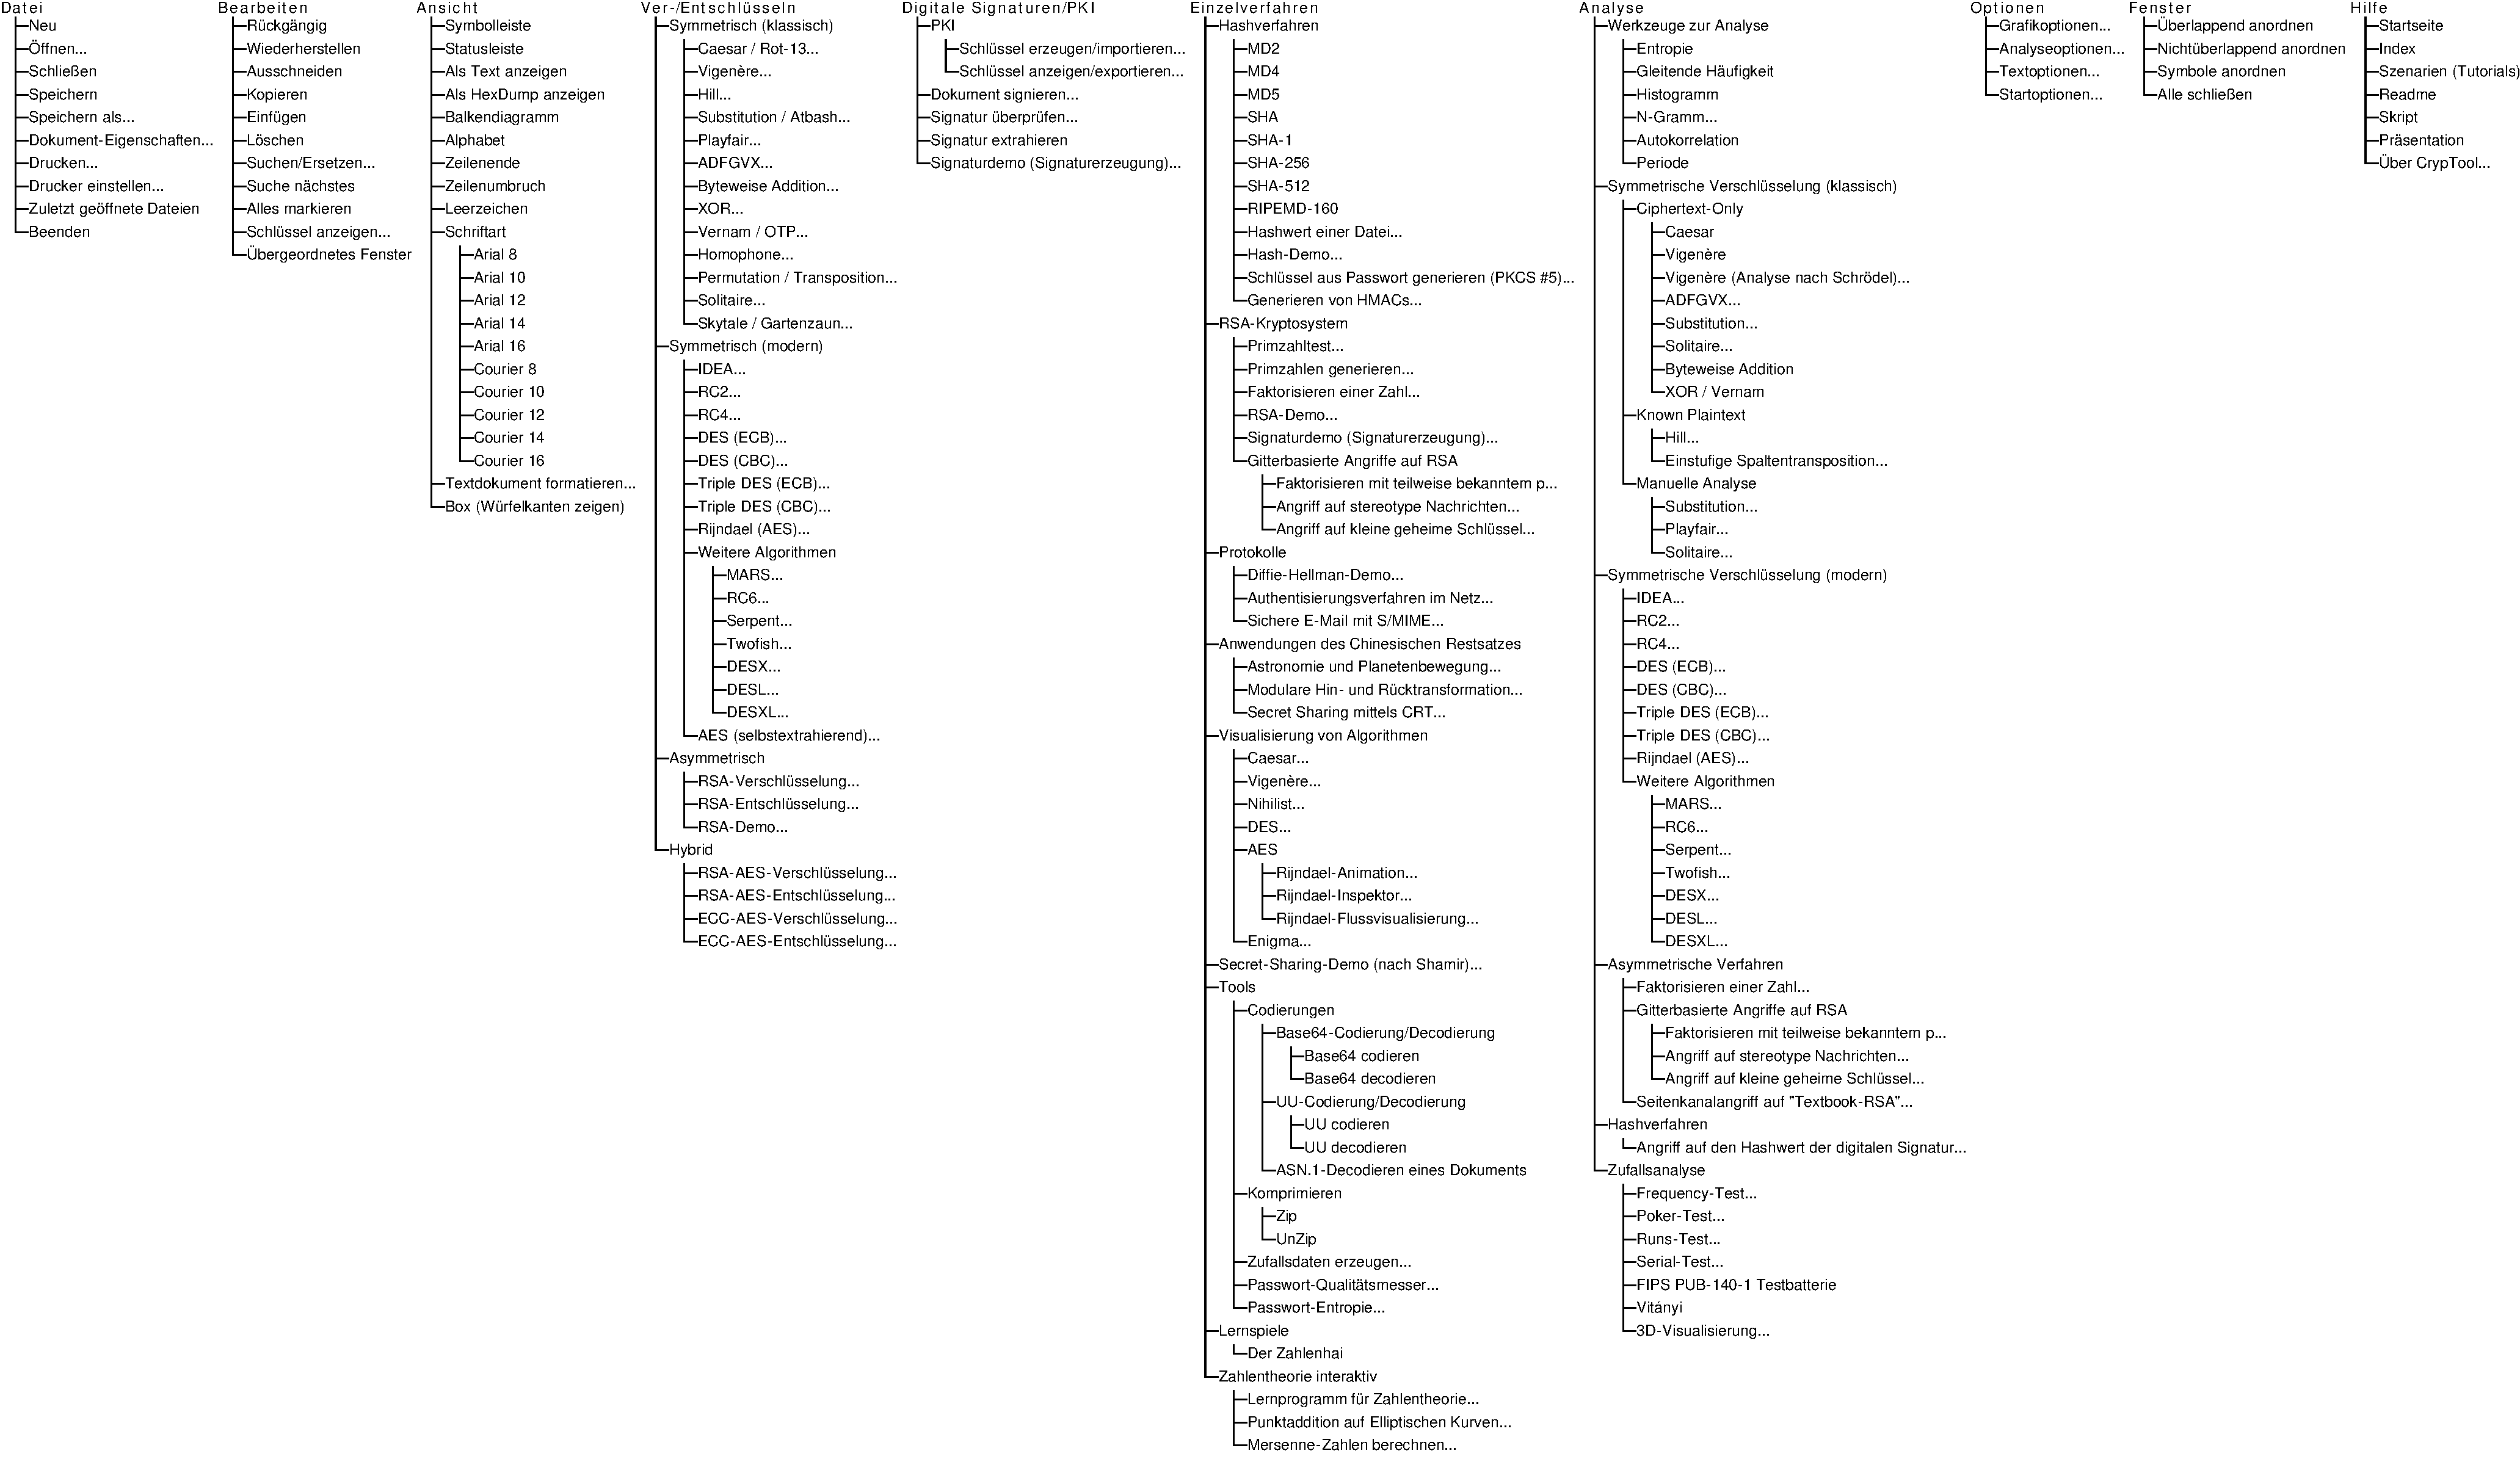
\includegraphics[scale=0.4]{figures/CT1-menutree-de}  % Ohne Runterskalieren
 % ist die Grafik zu gro�, und ragt �ber die sichtbare Minipage / Seite hinaus.
%} % Ende von \frame
\hypertarget{appendix-figure-menu-overview-CT1}{}
% \captionsetup[figure]{skip=110pt}  %%%% Tat nicht: Package caption Warning: Unused \captionsetup[figure]
\setlength{\abovecaptionskip}{5mm}  %%%% Tat, um den Abstand zwischen Bild und �berschrift zu �ndern
\caption{Komplett-�bersicht �ber den Men�-Baum von CT1 (CrypTool~1.4.31)}%TODO-xxxxxx(last update 1.4.31-final)
\label{appendix-figure-menu-overview-CT1}
\end{minipage}
}
}

\end{center}
\end{figure}

\clearpage
\setlength{\hoffset}{0mm}
%\restoregeometry
%\newgeometry{bottom=3.2cm} % Trotz restoregeometry ist die Seitennummer etwas nach oben geschoben.
                           % Aber wenn zus�tzlich neues geometry, gibt es Probleme, denn es macht
			   % bspw. den li. Rand breiter --> falsche Umbr�che. TODO-xxxxxxxxxxxxxxxxsofort



%--------------------------------------------------------------------
\newpage
%\enlargethispage{1cm}
\hypertarget{appendix-template-overview-CT2}{}
\section{CrypTool-2-Vorlagen}
\label{s:appendix-template-overview-CT2}

\noindent Dieser Anhang enth�lt auf den folgenden Seiten den Baum
mit allen Vorlagen in CrypTool~2\index{CT2}.\footnote{%
  Weitere Informationen zu CT2 finden Sie auf:
  \url{https://www.cryptool.org/de/ct2-dokumentation}
}

\noindent Beim Start von CT2 �ffnet sich das Startcenter.

%\clearpage
\begin{figure}[hb]
\begin{center}
%\vspace{-30pt}
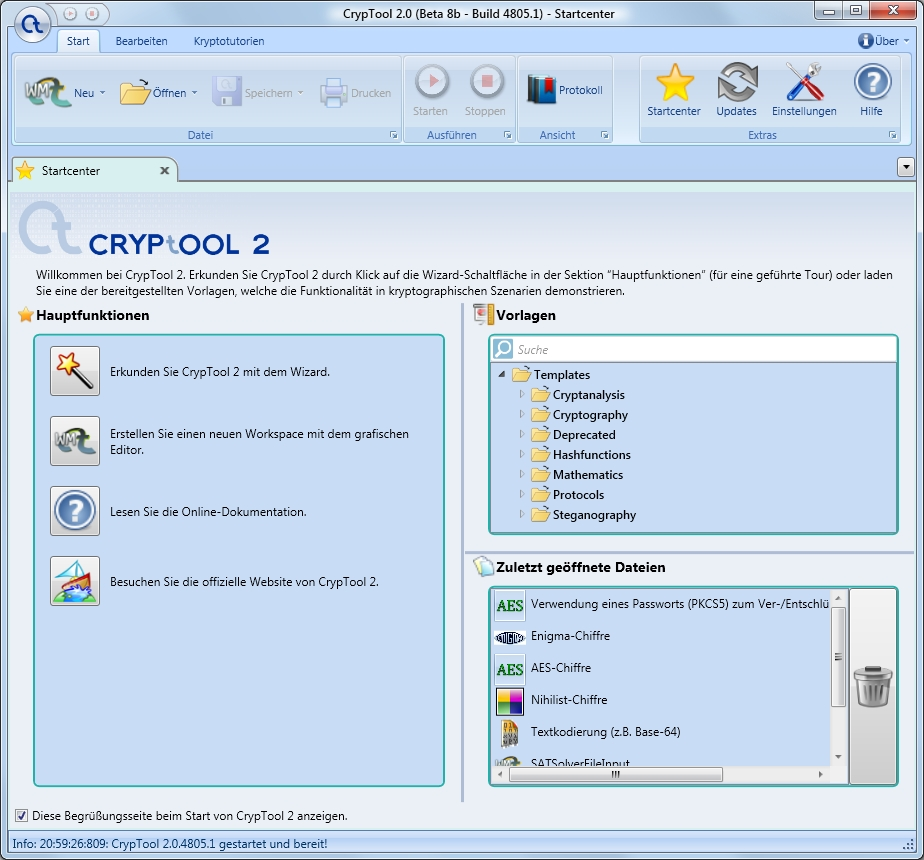
\includegraphics[scale=0.45, angle=0] {figures/CT2-Startcenter-de}
\hypertarget{Welcome-CT2}{}
\caption{Startcenter in CT2 (Beta 8b, Mai 2012)}
\label{Welcome-Screenshot-CT2}
\end{center}
\end{figure}
%\clearpage

\noindent Darin hat man die Auswahl, die Funktionalit�t auf drei verschiedenen Wegen aufzurufen:
\begin{itemize}
   \item �ber den Wizard: Er leitet einen gef�hrt zu den Funktionen.
   \item �ber die Arbeitsfl�che, auf der man die Komponenten (z.B. eine Verschl�sselungsfunktion, eine Texteingabefunktion, ...) anhand der visuellen Programmierung\index{visuelle Programmierung} selbst zusammenstellen kann.
   \item �ber den Vorlagen-Baum, aus dem man fertige Workflows ausw�hlen kann.
 \end{itemize}

Der Wizard stellt Fragen zu dem gew�nschten Szenario (z.B. Base64-Codierung) und f�hrt den Benutzer dann zu den Funktionen. Das gew�hlte Szeanrio mit den eigenen Eingaben kann man anschlie�end auch als Vorlage abspeichern.

Auf die leere Arbeitsfl�che kann man aus der linken Navigationsleiste alle Komponenten ziehen und diese dann wie gew�nscht miteinander verbinden. Die implementierte Krypto-Funktionalit�t steckt vor allem in diesen Komponenten (z.B. Enigma, AES).

Im Vorlagen-Baum gibt es zu jeder Komponente mindestens eine Vorlage. Die angebotenen Vorlagen enthalten sofort lauff�hige komplette Workflows. Wenn man z.B. in der Vorlage zu AES seine Eingaben �ndert, sieht man dynamisch und sofort, wie sich Ausgaben entsprechend �ndern (wie z.B. durch Padding ein Block hinzukommt, wie sich das Chaining auswirkt, ...).

\clearpage
\begin{figure}[hb]
\begin{center}
\vspace{-30pt}
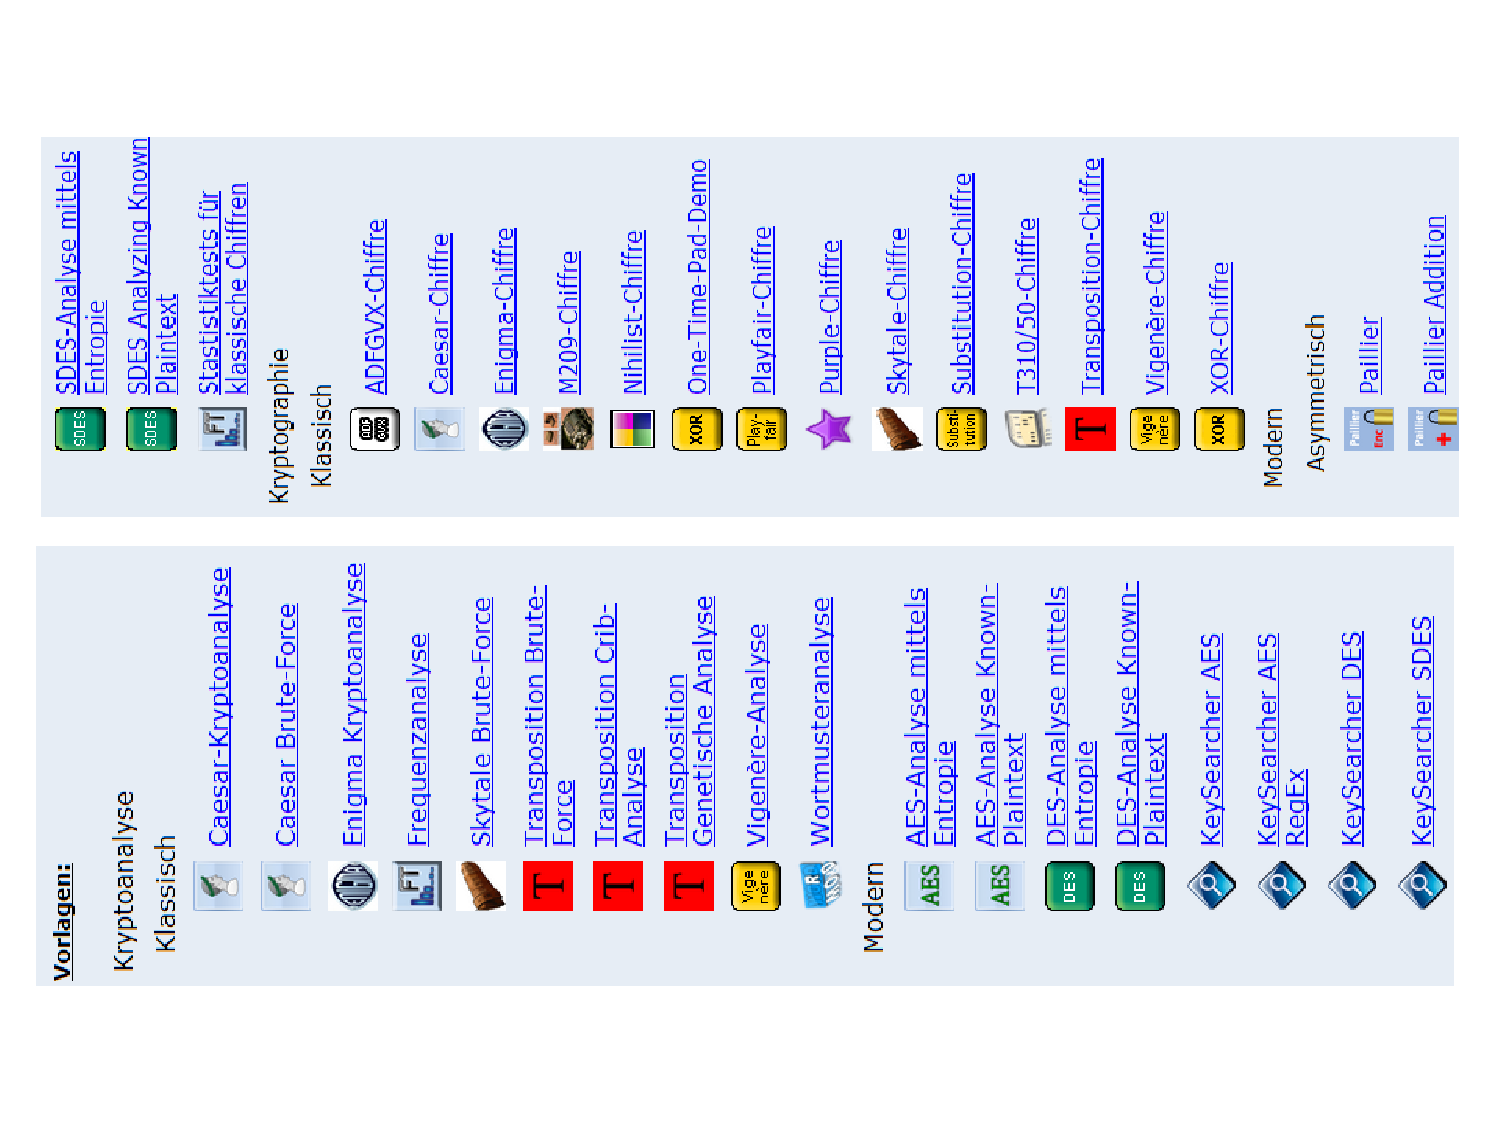
\includegraphics[scale=0.8, angle=270]
                {figures/CT2-templatetree-de-1}
\hypertarget{appendix-figure-template-overview-CT2}{}
\caption{Screenshot �ber den Template-Baum von CT2 (NB4882.1, Juli 2012), Teil 1}
\label{appendix-figure-template-overview-CT2}
% \hypertarget{appendix-figure-template-overview-CT2}{}
\end{center}
\end{figure}
\clearpage





%--------------------------------------------------------------------
\newpage
%\enlargethispage{1cm}
\hypertarget{appendix-function-overview-JCT}{}
\section{JCrypTool-Funktionen}
\label{s:appendix-function-overview-JCT}

\noindent Dieser Anhang enth�lt auf den folgenden Seiten eine Liste aller
Funktionen in JCrypTool\index{JCT}.\footnote{%
  Weitere Informationen zu JCT finden Sie auf:
  \url{http://www.cryptool.org/de/jct-machmit} \\
  Die Liste wurde mit Hilfe der CT-Portal-Webseite gewonnen.}

\noindent Beim ersten Start von JCT �ffnet sich das Willkommen-Fenster.

%\clearpage
\begin{figure}[hb]
\begin{center}
%\vspace{-30pt}
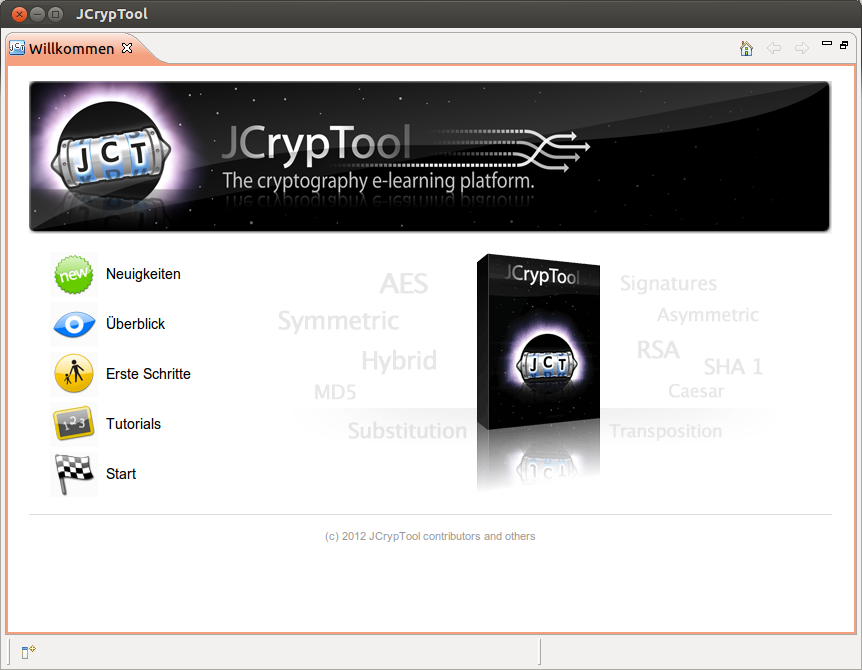
\includegraphics[scale=0.45, angle=0] {figures/JCT-Welcome-DE}
\hypertarget{Welcome-Screenshot-JCT}{}
\caption{Willkommen-Fenster in JCT (RC6, Juli 2012)}
\label{Welcome-Screenshot-JCT}
\end{center}
\end{figure}
%\clearpage
Mit Klick auf \glqq Start\grqq~kann man die verschiedenen Funktionen direkt nutzen.
Die in JCT implementierten Funktionen werden �ber zwei unterschiedliche Perspektiven angeboten:
\begin{itemize}
   \item Standard-Perspektive
   \item Algorithmen-Perspektive
 \end{itemize}

Alle Funktionen in der {\bf Standard-Perspektive} finden sich sowohl in den Men�s als
auch in der \glqq Krypto-Explorer\grqq~genannten Navigationsleiste (rechts). Die Standard-Perspektive enth�lt alle wichtigen Verfahren (wie z.B. die klassische Transposition oder den modernen AES)  und viele Visualisierungen (z.B. Diffie-Hellman-Schl�sselaustausch oder Berechnungen auf Elliptischen Kurven).

Alle Funktionen der {\bf Algorithmen-Perspektive} finden sich in der \glqq Algorithmen\grqq~genannten Navigationsleiste (in dieser Perspektive ebenfalls rechts). Die Algorithmen-Perspektive enth�lt alle Detaileinstellungen der verschiedenen Algorithmen und bietet insbesondere auch Algorithmen aus dem Bereich des Post-Quantum-Computings\index{Post-Quantum-Computing} (PQC) an.

\clearpage
\begin{figure}[hb]
\begin{center}
\vspace{-30pt}
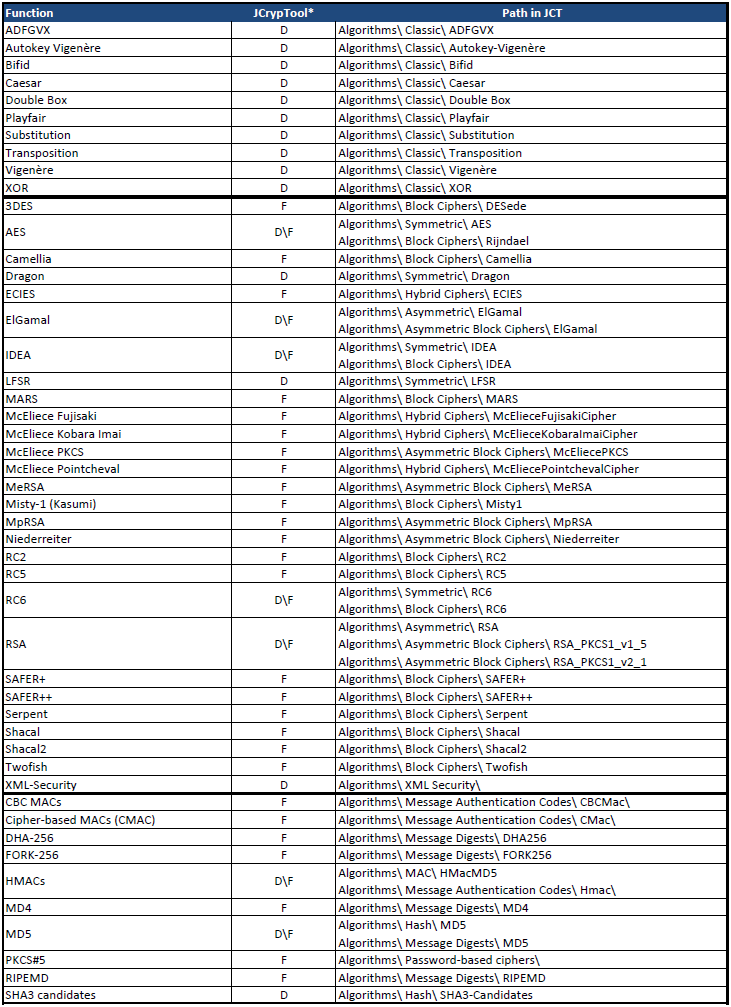
\includegraphics[scale=0.8, angle=0] {figures/JCT-functions-de-1}
\hypertarget{functions-overview-1-JCT}{}
\caption{Screenshot zu den Funktionen in JCT (RC6, Juli 2012), Teil 1}
\label{functions-overview-1-JCT}
\end{center}
\end{figure}
\clearpage

\clearpage
\begin{figure}[hb]
\begin{center}
\vspace{-30pt}
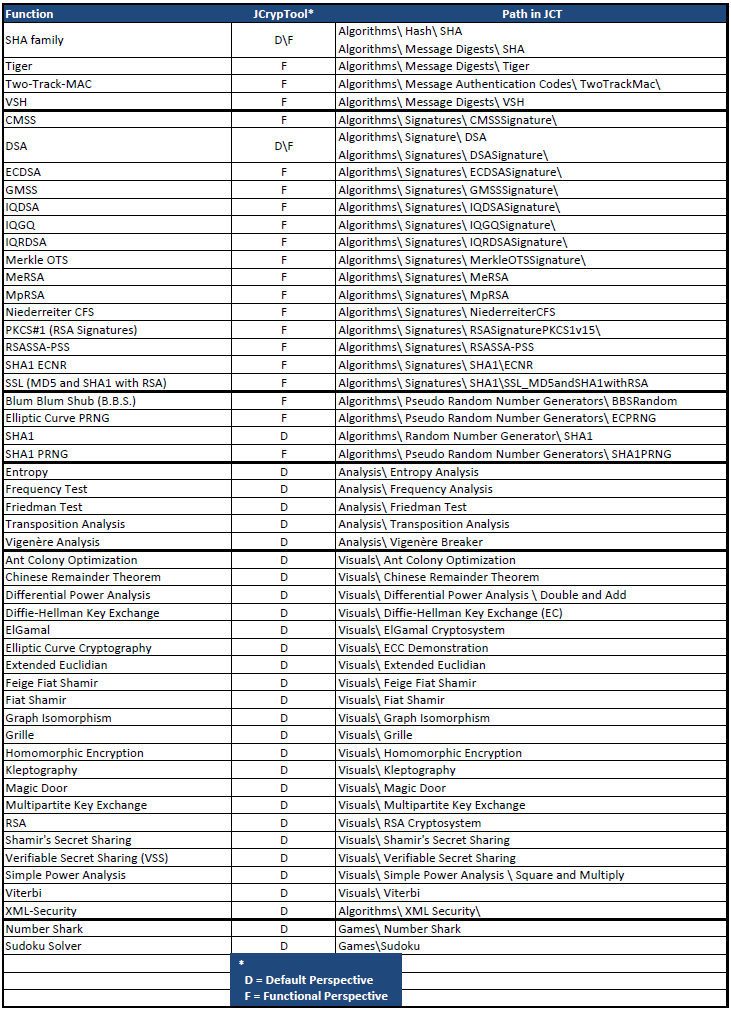
\includegraphics[scale=0.8, angle=0] {figures/JCT-functions-de-2}
\hypertarget{functions-overview-2-JCT}{}
\caption{Screenshot zu den Funktionen in JCT (RC6, Juli 2012), Teil 2}
\label{functions-overview-2-JCT}
\end{center}
\end{figure}
\clearpage





%--------------------------------------------------------------------
\newpage
%\enlargethispage{1cm}
\hypertarget{appendix-function-overview-CTO}{}
\section{CrypTool-Online-Funktionen}
\label{s:appendix-function-overview-CTO}

\noindent Dieser Anhang enth�lt eine Liste aller
Funktionen in CrypTool-Online (CTO)\index{CTO}.\footnote{%
  Weitere Informationen zu CTO finden Sie auf:
  \url{www.cryptool-online.org} \\
  Die Liste wurde mit Hilfe der Funktionsliste auf der CT-Portal-Webseite gewonnen:\\
  \url{https://www.cryptool.org/de/ctp-dokumentation/ctp-funktionsumfang}}


%\noindent Die Einstiegsseite von CTO sieht so aus:
%\clearpage
%\begin{figure}[hb]
%\begin{center}
%\vspace{-30pt}
%\includegraphics[scale=0.45, angle=0] {figures/CTO-Welcome-DE}
%\hypertarget{Welcome-Screenshot-CTO}{}
%\caption{Einstiegsseite in CrypTool-Online (November 2012)}
%\label{Welcome-Screenshot-CTO}
%\end{center}
%\end{figure}
%\clearpage


\noindent Der folgende Screenshot zeigt die auf CTO implementierten
Krypto-Funktionen:
\clearpage
\begin{figure}[hb]
\begin{center}
\vspace{-30pt}
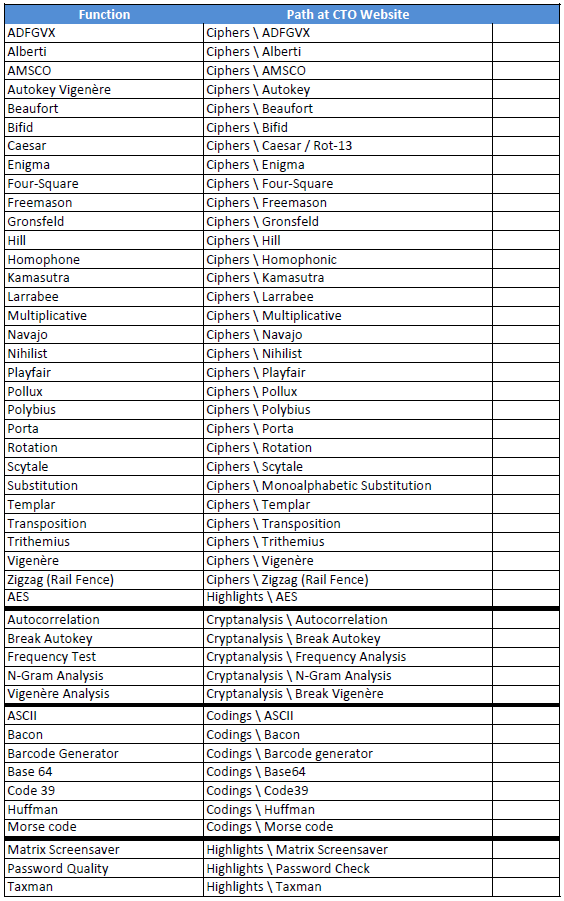
\includegraphics[scale=0.8, angle=0] {figures/CTO-functions-de-1}
\hypertarget{functions-overview-1-CTO}{}
\caption{Screenshot zu den Funktionen in CTO (November 2012)}
\label{functions-overview-1-CTO}
\end{center}
\end{figure}
\clearpage

%\clearpage
%\begin{figure}[hb]
%\begin{center}
%\vspace{-30pt}
%\includegraphics[scale=0.8, angle=0] {figures/CTO-functions-de-2}
%\hypertarget{functions-overview-2-CTO}{}
%\caption{Screenshot zu den Funktionen in CTO (November 2012), Teil 2}
%\label{functions-overview-2-CTO}
%\end{center}
%\end{figure}
%\clearpage


  \renewcommand{\CTBChapName}{(Appendix LearnTool)}  % $Id:
% !Mode:: "TeX:DE"    % Setting document mode and submode for WinEdt
% ..............................................................................
%             F I L M E  +  R O M A N E
% ~~~~~~~~~~~~~~~~~~~~~~~~~~~~~~~~~~~~~~~~~~~~~~~~~~~~~~~~~~~~~~~~~~~~~~~~~~~~~~
%
% Consider to add next time:
%  - Filme: Matrix, Tron, Echelon Verschwörung, ...
%  - Bücher: xxx, ...
% ~~~~~~~~~~~~~~~~~~~~~~~~~~~~~~~~~~~~~~~~~~~~~~~~~~~~~~~~~~~~~~~~~~~~~~~~~~~~~~


\begin{refsegment}

\newpage
\hypertarget{appendix-movies}{}
\section{Filme und belletristische Literatur mit Bezug zur Kryptographie}
\label{s:appendix-movies}
% {\bf Filme und Literatur mit Bezug zur Kryptographie} (siehe Anhang \ref{s:appendix-movies})
\index{Filme}
\index{Literatur}


Kryptographische Verfahren -- sowohl klassische wie moderne -- fanden auch
Eingang in die Literatur und in Filme. In manchen Medien werden diese nur
erwähnt und sind reine Beigabe, in anderen sind sie tragend und werden
genau erläutert, und manchmal ist die Rahmenhandlung nur dazu da, dieses
Wissen motivierend zu transportieren. Anbei der Beginn eines Überblicks.

% --------------------------------------------------------------------------
\subsection{Für Erwachsene und Jugendliche}
\label{s:Light-fiction-for-grownups}

%be_2005: Hatte zuerst \begin{thebibliography}{99999} und \bibitem[... ,
%         aber dann wurde immer der feste Titel "Literatur" bzw. "References"
%         geschrieben und wir fanden keine Möglichkeit, ihn weg zu bekommen.
%         Lösung: Stattdessen \begin{description} \item[...


\begin{description}

\item[\textrm{[Poe1843]}] \index{Poe 1843}
    Edgar Allan Poe\index{Poe, Edgar Allan}, \\
    {\em Der Goldkäfer}, 1843.\footnote{%
        Siehe \url{https://de.wikipedia.org/wiki/Der_Goldk%C3%A4fer}.

	Eine didaktisch aufbereitete Beschreibung zum Einsatz im Schulunterricht findet
        sich in Teil 1 der Artikelserie {\em RSA \& Co. in der Schule:
        Moderne Kryptologie, alte Mathematik, raffinierte Protokolle}.
        Siehe \cite{Witten1998}, S. 52 ff (\glqq Das Gold des Gehenkten\grqq).
	\index{RSA \& Co. in der Schule}

	Alle Materialien zu der Goldkäfer-Unterrichtsstunde (oder Doppelstunde)
	finden sich unter \url{http://www.informatik-im-kontext.de/} via
	\glqq E-Mail (nur?) für Dich\grqq~=> \glqq Vertraulichkeit mit Verschlüsselungsverfahren\grqq.
	% In den Materialien wird ein erprobter generischer Gang zu RSA präsentiert:
	% Monoalphabetische Verschlüsselung (Goldkäfer) => Knacken durch Häufigkeitsanalyse
	% => polyalphabetische Verschlüsselung => Knacken durch Bestimmung der Schlüssellänge (Kasiski, Friedman)
	% => One-Time-Pad als beweisbar sicheres Verschlüsselungsverfahren
	% => Problem des Schlüsselmanagments => asymmetrische Kryptographie (Diffie, Hellman, Merkle, RSA).

	Poe war nicht nur ein bekannter -- in seiner Heimat Amerika zunächst
	verkannter -- Schriftsteller und Erfinder des Kriminalromans,
	%% („Der Doppelmord in der Rue Morgue“, s. https://de.wikipedia.org/wiki/Edgar_Allan_Poe,
	%% https://de.wikipedia.org/wiki/Der_Doppelmord_in_der_Rue_Morgue)
	sondern auch ein begabter Kryptologe. Die Geschichte dazu wird auch in dem
	Krypto-Buch {\em Verschlüsselte Botschaften} \cite{Kippenhahn1997}
	erzählt.
    }\\
    Diese Kurzgeschichte erschien in Deutsch z.B. in der illustrierten und
    mit Kommentaren in den Marginalspalten versehenen Ausgabe "`Der Goldkäfer
    und andere Erzählungen"', Gerstenbergs visuelle Weltliteratur,
    Gerstenberg Verlag, Hildesheim, 2002.\\
    In dieser Kurzgeschichte beschreibt Poe als Ich-Erzähler seine
    Bekanntschaft mit dem sonderbaren Legrand. Mit Hilfe eines an der
    Küste Neuenglands gefundenen Goldkäfers, einem alten Pergament und
    den Dechiffrierkünsten von Legrand finden Sie den sagenhaften Schatz
    von Kapitän Kidd.\\
    Die Geheimschrift besteht aus 203 kryptischen Zeichen und erweist sich
    als allgemeine monoalphabetische Substitutions-Chiffre (vgl.
    Kapitel~\ref{monoalphabeticSubstitutionCiphers}). Ihre schrittweise
    Dechiffrie"-rung durch semantische und syntaktische Analyse
    (Häufigkeit der einzelnen Buchstaben in englischen Texten)
    wird in der Geschichte ausführlich erläutert.\footnote{%
      Teil der oben genannten Unterrichtsmaterialien ist auch ein Python-Programm.\index{Python}
      %% Außerdem gibt es eine schrittweise Lösung des Gold-Bug-Kryptogramms,
      %% das vor einigen Jahren Wittens Frau in Standard-HTML schrieb.
      Damit lässt sich das Kryptogramm mit Python {\em und} mit SageMath\index{SageMath}
      entschlüsseln.
      Siehe das Code-Beispiel in \ref{s:appendix-Code-for-light-fiction-books}.
      % \ref{Lit_Python-sample_Gold-bug}  Hier druckt er "A.1" ?
    }\\
    Der Entschlüsseler Legrand sagt darin (S. 39) den berühmten Satz:
    "`Und es ist wohl sehr zu bezweifeln, ob menschlicher Scharfsinn
    ein Rätsel ersinnen kann, das menschlicher Scharfsinn bei
    entsprechender Hingabe nicht wieder zu lösen vermag."'\\
    % D: Poe: 1809-1849, "Vater des Kriminalromans", er schloss Wetten ab,
    % dass er alle verschlüsselten Botschaften, die ihm Freunde und Leser
    % vorlegten, im Handumdrehen entschlüsseln könne. Gutes Gespür durch
    % viel Übung.
    % E: Poe, 1809-1849 was named "Father of the crime novel". He claimed,
    % that he will be able to decrypt any cipher sent to him by friends or
    % readers.
    %
    % Originalausgabe dieser illustrierten Ausgabe: "Le scarabée d'or et
    %                           autre nouvelles", Gallimard, Paris, 1998.
    % In "Der Goldkäfer" wird detailliert beschrieben, wie der verarmte
    % Hugenotte William Legrand in South Carolina die monoalphabetische
    % Geheimschrift des Piratenkapitäns Kidd knackt, die zu einem
    % sagenhaften Schatz führt.


\item[\textrm{[Verne1885]}] \index{Verne 1885}
    Jules Verne\index{Verne, Jules}, \\
    {\em Mathias Sandorf}, 1885. \\
    Dies ist einer der bekanntesten Romane des französischen Schriftstellers
    Jules Verne (1828-1905), der auch als "`Vater der Science Fiction"'
    bezeichnet wurde.\\
    Erzählt wird die spannende Geschichte des Freiheitskämpfers Graf
    Sandorf, der an die Polizei verraten wird, aber schließlich fliehen
    kann.\\
    Möglich wurde der Verrat nur, weil seine Feinde eine Geheimbotschaft an
    ihn abfangen und entschlüsseln konnten. Dazu benötigten sie eine
    besondere Schablone, die sie ihm stahlen. Diese Schablone bestand aus
    einem quadratischen Stück Karton mit 6x6 Kästchen, wovon 1/4, also neun,
    ausgeschnitten waren (vgl. die
    \hyperlink{turning-grille-cipher}{Fleißner-Schablone}
    in Kapitel~\ref{introsamplesTranspositionCiphers}).\\


    % Gefunden in: CRYPTO-GRAM, January 15, 2007, by Bruce Schneier
\item[\textrm{[Kipling1901]}] \index{Kipling 1901}
    Rudyard Kipling\index{Kipling, Rudyard}, \\
    {\em Kim}, 1901. \\
    Dieser Roman wird in der Besprechung von Rob Slade%
    \footnote{Siehe
      % \href{http://catless.ncl.ac.uk/Risks/24.49.html\#subj12} %% \ vor # nötig !
        \url{http://catless.ncl.ac.uk/Risks/24.49.html#subj12}.
    }
    folgendermaßen beschrieben:
    "`Kipling packte viele Informationen und Konzepte in seine Geschichten.
    In "`Kim"' geht es um das große "`Spiel"' Spionage und Bespitzelung.
    Schon auf den ersten 20 Seite finden sich Authentisierung über Besitz,
    Denial of Service, Sich-für-jemand-anderen-Ausgeben (Impersonation),
    Heimlichkeit, Maskerade, Rollen-basierte Autorisierung (mit
    Ad-hoc-Authentisierung durch Wissen), Abhören, und Vertrauen basierend
    auf Datenintegrität.
    Später kommen noch Contingency Planning gegen Diebstahl und
    Kryptographie mit Schlüsselwechsel hinzu."'\\
    Das Copyright des Buches ist abgelaufen.%
    \footnote{Sie können es lesen unter:\\
          \url{http://kipling.thefreelibrary.com/Kim} oder\\
          \url{http://www.readprint.com/work-935/Rudyard-Kipling}.
    }\\


\item[\textrm{[Doyle1905]}] \index{Doyle 1905}
    Arthur Conan Doyle\index{Doyle, Sir Arthur Conan}, \\
    {\em Die tanzenden Männchen}, 1905. \\
    In der Sherlock-Holmes-Erzählung {\em Die tanzenden Männchen}
    (erschienen erstmals 1903 im "`Strand Magazine"', und dann 1905 im
    Sammelband "`Die Rückkehr des Sherlock Holmes"' erstmals in Buchform)
    wird Sherlock Holmes mit einer Geheimschrift konfrontiert, die zunächst
    wie eine harmlose Kinderzeichnung aussieht. \\
    Sie erweist sich als monoalphabetische Substitutions-Chiffre (vgl.
    Kapitel~\ref{monoalphabeticSubstitutionCiphers}) des Verbrechers Abe
    Slaney. Holmes knackt die Geheimschrift mittels Häufigkeitsanaly"-se.\\


\item[\textrm{[Sayers1932]}] \index{Sayers 1932}
    Dorothy L. Sayers, \\
    {\em Zur fraglichen Stunde und Der Fund in den Teufelsklippen
    (Orginaltitel: Have his carcase)}, Harper, 1932 \\
    (Erste dt. Übersetzung {\em Mein Hobby: Mord} bei A. Scherz, 1964; \\
    dann {\em Der Fund in den Teufelsklippen} bei Rainer Wunderlich-Verlag,
    1974;\\
    Neuübersetzung 1980 im Rowohlt-Verlag). \\
    In diesem Roman findet die Schriftstellerin Harriet Vane eine Leiche
    am Strand und die Polizei hält den Tod für einen Selbstmord.
    Doch Harriet Vane und der elegante Amateurdetektiv Lord Peter Wimsey
    klären in diesem zweiten von Sayers's berühmten Harriet Vane's
    Geschichten den widerlichen Mord auf. \\
    Dazu ist ein Chiffrat zu lösen. Erstaunlicherweise beschreibt der
    Roman nicht nur detailliert die Playfair-Chiffre, sondern auch deren
    Kryptoanalyse (vgl. \hyperlink{playfair}{Playfair}
    in Kapitel~\ref{polygraphicSubstitutionCiphers}).\\


\item[\textrm{[Simmel1970]}] \index{Simmel 1970}
    Johannes Mario Simmel, \\
    {\em Und Jimmy ging zum Regenbogen}, Knaur Verlag, 1970. \\
    Der Roman spielt zwischen 1938 und
    1969 in Wien. Der Held Manuel Aranda deckt -- von mehreren Geheimdiensten
    verfolgt -- im Laufe der Handlung Stück für Stück die Vergangenheit seines
    ermordeten Vaters auf. Ein wichtiger Mosaikstein ist dabei ein
    verschlüsseltes Manuskript, das in Kapitel 33 entschlüssselt wird.
    Im Roman wird der Code als ein
    "`fünfundzwanzigfacher Caesar Code"' beschrieben, tatsächlich ist es eine
    Vigenère-Chiffre mit einem 25 Buchstaben langen Schlüssel. \\
    Das Buch wurde 1971 verfilmt.\\


\item[\textrm{[Crichton1988]}] \index{Crichton 1988}
    Michael Crichton, \\
    {\em Die Gedanken des Bösen (Orginaltitel: Sphere)}, Rororo, 1988. \\
    Ein Team verschiedener Wissenschaftler wird auf den Meeresgrund geschickt,
    um ein 900~m langes hoch entwickeltes Raumschiff zu untersuchen. Die
    Eigenheiten und psychischen Probleme der Forscher treten durch lebensbedrohliche
    Ereignisse und ihr Abgeschnittensein von oben immer mehr in den Vordergrund.
    Es gibt viele Rätsel: Das Raumschiff liegt schon 300 Jahre da, es hat
    englische Beschriftungen, es führt scheinbar ein Eigenleben, die menschliche
    Vorstellungskraft materialisiert sich. Unter anderem erscheint auf dem
    Bildschirm ein im Buch vollständig abgedruckter Code, der von dem genialen
    Mathematiker Harry entschlüsselt werden kann: ein einfacher spiralenförmiger
    Ersetzungscode.\\


\item[\textrm{[Seed1990]}] \index{Seed 1990}
    Regie Paul Seed (Paul Lessac), \\
    {\em Das Kartenhaus (Orginaltitel: House of Cards)}, 1990 (dt. 1992). \\
    In diesem Film versucht Ruth, hinter das Geheimnis zu kommen, das ihre
    Tochter verstummen ließ. Hierin unterhalten sich Autisten mit Hilfe von
    5- und 6-stelligen Primzahlen (siehe
    Kapitel~\ref{Chapter_Primes}).
    Nach über eine Stunde kommen im Film die folgenden beiden (nicht
    entschlüsselten) Primzahlfolgen vor:
%  \vskip -30pt  %be_2005 Bewirkt anscheinend nichts -- Abstand etwas zu groß.
    \begin{center}
    $21.383, \;\;176.081, \;\;18.199, \;\;113.933, \;\;150.377, \;\;304.523, \;\;113.933$\\
    $193.877, \;\;737.683, \;\;117.881, \;\;193.877$
    \end{center}
    \vskip +10 pt   % da "\\" hier nicht geht!


\item[\textrm{[Robinson1992]}] \index{Robinson 1992}
    Regie Phil Alden Robinson, \\
    {\em Sneakers - Die Lautlosen (Orginaltitel: Sneakers)},
    Universal Pictures Film, 1992. \\
    In diesem Film versuchen die "`Sneakers"' (Computerfreaks um ihren Boss
    Martin Bishop), den "`Bösen"' das Dechiffrierungsprogramm SETEC abzujagen.
    SETEC wurde von einem genialen Mathematiker vor seinem gewaltsamen Tod
    erfunden und kann alle Geheimcodes dieser Welt entschlüsseln.\\
    In dem Film wird das Verfahren nicht beschrieben%
    \footnote{
       An dem Film hatte Leonard Adleman (das "`A"' von RSA) als mathematischer
       Berater mitgearbeitet. Die recht lustige Geschichte über seine Mitwirkung
       bei Sneakers beschreibt er selbst auf seiner Homepage unter
       %% BE_8.8.18: Link tot: \url{http://www.usc.edu/dept/molecular-science/fm-sneakers.htm}.
       \url{http://world.std.com/~reinhold/math/sneakers.adleman.html}.
       Man kann man davon ausgehen, dass es sich bei dem überall benutzten
       Verschlüsselungsverfahren um RSA handelt.
       In dem Chip ist demnach ein bis dahin unbekanntes, schnelles
       Faktorisierungsverfahren\index{Faktorisierung} implementiert.
    }.\\


\item[\textrm{[Baldacci1997]}] \index{Baldacci 1997}
    David Baldacci, \\
    {\em Das Labyrinth. Total Control}, Lübbe, 1997. \\
    Jason Archer, Direktor einer Technologie-Firma, verschwindet plötzlich.
    Seine Frau Sidney Archer versucht, den Grund seines plötzlichen Todes
    herauszufinden, und entdeckt, wie das Finanzsystem missbraucht wird und
    dass die reale Macht bei denen mit dem meisten Geld liegt. Hier helfen
    dann auch gute Passworte nicht...\\


\item[\textrm{[Natali1997]}] \index{Natali 1997}
    Regie Vincenzo Natali, \\
    {\em Cube (Orginaltitel: Sneakers)},
    Mehra Meh Film, 1997. \\
    In diesem kanadischen Low-Budget-Film finden sich 7 sehr unterschiedliche
    Personen in einem endlos scheinenden Labyrinth von würfelartigen Räumen.\\
    Die Personen wollen nach draußen, müssen dazu aber die Räume durchqueren,
    von denen manche tödliche Fallen darstellen. Um herauszufinden, welche
    Räume gefährlich sind, spielt Mathematik eine entscheidende Rolle: Jeder
    Raum hat am Eingang eine Folge von 3 mal 3 Ziffern. Zuerst nehmen
    sie an, dass alle Räume Fallen sind, wo wenigstens eine der 3 Zahlen eine
    Primzahl ist. Später stellt sich heraus, dass auch alle diejenigen Räume
    Fallen sind, bei denen eine der 3 Zahlen eine Potenz von genau einer
    Primzahl ist (Fallen sind also $p^n$, z.B. $128=2^7$ oder
    $101 = 101^1 = prim$, aber nicht $517 = 11*47$).\\


\item[\textrm{[Becker1998]}] \index{Becker 1998}
    Regie Harold Becker, \\
    {\em Das Mercury Puzzle (Orginaltitel: Mercury Rising)},
    Universal Pictures Film, 1998. \\
    Die NSA hat einen neuen Code entwickelt, der angeblich weder von Menschen
    noch von Computern geknackt werden kann. Um die Zuverlässigkeit zu testen,
    verstecken die Programmierer eine damit verschlüsselte Botschaft in
    einem Rätselheft.\\
    Simon, eine neunjähriger autistischer Junge, knackt den Code.
    Statt den Code zu fixen, schickt ihm ein Sicherheitsbeamter einen Killer.
    Der FBI-Agent Art Jeffries (Bruce Willis) beschützt den Jungen und
    stellt den Killern eine Falle.\\
    Das Chiffrier-Verfahren wird nicht beschrieben.\\


\item[\textrm{[Brown1998]}] \index{Brown 1998}
    Dan Brown, \\
    {\em Diabolus (Orginaltitel: Digital Fortress)}, Lübbe, 2005. \\
    Dan Browns erster Roman "`The Digital Fortress"' erschien 1998 als E-Book,
    blieb jedoch damals weitgehend erfolglos.\\
    Die National Security Agency (NSA) hat für mehrere Milliarden US-Dollar
    einen gewaltigen Computer gebaut, mit dem sie in der Lage ist, auch nach
    modernsten Verfahren verschlüsselte Meldungen (natürlich nur die von
    Terroristen und Verbrechern) innerhalb weniger Minuten zu entziffern.\\
    Ein abtrünniger Angestellter erfindet einen unbrechbaren Code und
    sein Computerprogramm Diabolus zwingt damit den Supercomputer zu
    selbstzerstörerischen Rechenoperationen. Der Plot, in dem auch die
    schöne Computerexpertin Susan Fletcher eine Rolle spielt, ist ziemlich
    vorhersehbar.\\
    Die Idee, dass die NSA oder andere Geheimdienste jeden Code knacken
    können, wurde schon von mehreren Autoren behandelt: Hier hat der
    Supercomputer 3 Millionen Prozessoren -- trotzdem ist es aus heutiger
    Sicht damit auch nicht annäherungsweise möglich, diese modernen Codes
    zu knacken.\\


\item[\textrm{[Elsner1999]}] \index{Elsner 1999}
    Dr.~C.~Elsner, \\
    {\em Der Dialog der Schwestern}, c't, Heise-Verlag, 1999. \\
    In dieser Geschichte, die dem CrypTool-Paket\index{CrypTool} als PDF-Datei
    beigelegt ist, unterhalten sich die Heldinnen vertraulich mit einer
    Variante des RSA-Verfahrens (vgl. Kapitel~\ref{rsabeweis} ff.).
    Sie befinden sich in einem Irrenhaus unter ständiger Bewachung.\\


\item[\textrm{[Stephenson1999]}] \index{Stephenson 1999}
    Neal Stephenson, \\
    {\em Cryptonomicon}, Harper, 1999. \\
    Der sehr dicke Roman beschäftigt sich mit Kryptographie sowohl im
    zweiten Weltkrieg als auch in der Gegenwart.
    Die zwei Helden aus den 40er-Jahren sind der glänzende Mathematiker und
    Kryptoanalytiker Lawrence Waterhouse, und der übereifrige,
    morphiumsüchtige Bobby Shaftoe von den US-Marines.
    Sie gehören zum Sonderkommando 2702, einer Alliiertengruppe, die
    versucht, die gegnerischen Kommunikationscodes zu knacken und dabei
    ihre eigene Existenz geheim zu halten. \\
    In der Gegenwartshandlung tun sich die Enkel der Weltkriegshelden -- der
    Programmierfreak Randy Waterhouse und die schöne Amy Shaftoe -- zusammen. \\
    Cryptonomicon ist für nicht-technische Leser teilweise schwierig zu
    lesen. Mehrere Seiten erklären detailliert Konzepte der Kryptographie.
    Stephenson legt eine ausführliche Beschreibung der Solitaire-Chiffre
    (siehe Kapitel~\ref{Further-PaP-methods}) bei, ein
    Papier- und Bleistiftverfahren\index{Papier- und Bleistiftverfahren},
    das von Bruce Schneier entwickelt wurde und im
    Roman "`Pontifex"' genannt wird. Ein anderer, moderner Algorithmus
    namens "`Arethusa"' wird dagegen nicht offengelegt.\\


\item[\textrm{[Elsner2001]}] \index{Elsner 2001}
    Dr.~C.~Elsner, \nopagebreak\\
    {\em Das Chinesische Labyrinth}, c't, Heise-Verlag, 2001. \\
    In dieser Geschichte, die dem CrypTool-Paket\index{CrypTool} als PDF-Datei
    beigelegt ist, muss Marco Polo in einem Wettbewerb Probleme aus der
    Zahlentheorie lösen, um Berater des großen Khan zu werden. Alle Lösungen
    sind angefügt und erläutert.\\


\item[\textrm{[Colfer2001]}] \index{Colfer 2001}
    Eoin Colfer, \\
    {\em Artemis Fowl}, List-Verlag, 2001. \\
    In diesem Jugendbuch gelangt der junge Artemis, ein Genie und Meisterdieb,
    an eine Kopie des streng geheimen "`Buches der Elfen"'. Nachdem er es mit
    Computerhilfe entschlüsselt hat, erfährt er Dinge, die kein Mensch
    erfahren dürfte. \\
    Der Code wird in dem Buch nicht genauer beschrieben.\\


\item[\textrm{[Howard2001]}] \index{Howard 2001}
    Regie Ron Howard, \\
    {\em A Beautiful Mind}, 2001. \\
    Verfilmung der von Sylvia Nasar verfassten Biographie des
    Spieltheoretikers John Nash.
    Nachdem der brillante, aber unsoziale Mathematiker geheime kryptographische
    Arbeiten annimmt, verwandelt sich sein Leben in einen Alptraum. Sein
    unwiderstehlicher Drang, Probleme zu lösen, gefährden ihn und sein
    Privatleben.
    Nash ist in seiner Vorstellungswelt ein staatstragender Codeknacker. \\
    Konkrete Angaben zur seinen Analyseverfahren werden nicht beschrieben.\\


\item[\textrm{[Apted2001]}] \index{Apted 2001}
    Regie Michael Apted, \\
    {\em Enigma -- Das Geheimnis}, 2001. \\
    Verfilmung des von Robert Harris verfassten "`historischen Romans"'
    {\em Enigma} (Hutchinson, London, 1995) über die berühmteste
    Verschlüsselungsmaschine in der Geschichte, die in
    Bletchley Park nach polnischen Vorarbeiten gebrochen wurde.
    Die Geschichte spielt 1943, als der eigentliche Erfinder Alan Turing
    schon in Amerika war. So kann der Mathematiker Tom Jericho als Hauptperson
    in einem spannenden Spionagethriller brillieren.\\
    Konkrete Angaben zu dem Analyseverfahren werden nicht gemacht.\\


\item[\textrm{[Isau2003]}] \index{Isau 1997}
    Ralf Isau, \\
    {\em Das Museum der gestohlenen Erinnerungen}, Thienemann-Verlag, 1997/2003. \\
    Ein sehr spannender, hervorragend recherchierter und doch leicht zu lesender
    Roman mit einem tiefen Hintersinn.\\
    Als die Zwillinge Oliver und Jessica von ihren Ferien zurückkommen, haben sie
    ihren Vater vergessen. Die Realität verschiebt sich und niemand scheint es zu
    bemerken. An einigen Stellen bleiben manchmal Spuren zurück, die man
    entziffern kann.
    Zentrum der Geschichte ist das Ischtar-Tor im Berliner Pergamon-Museum.
    Nur mit dem Scharfsinn einer irischen Professorin (die gleichzeitig
    Computerexpertin, Archäologin und Philologin ist), den besonderen
    Beziehungen zwischen Zwillingen und den vereinten Kräften der
    Computergemeinschaft kann der letzte Teil des Spruches gelöst werden.\\
    Das Buch wurde als bestes Jugendbuch ausgezeichnet und liegt in 8 Sprachen vor.\\


\item[\textrm{[Brown2003]}] \index{Brown 2003}
    Dan Brown, \\
    {\em Sakrileg (Orginaltitel: The Da Vinci Code)}, Lübbe, 2004. \\
    Der Direktor des Louvre wird in seinem Museum vor einem Gemälde Leonardos
    ermordet aufgefunden, und der Symbolforscher Robert Langdon gerät in eine
    Verschwörung.\\
    Innerhalb der Handlung werden verschiedene klassische Chiffren (Substitution
    wie z.B. Caesar oder Vigen\`ere, sowie Transposition und Zahlencodes)
    angesprochen. Außerdem klingen interessante Nebenbemerkungen über
    Schneier oder die Sonnenblume an.
    Der zweite Teil des Buches ist sehr von theologischen Betrachtungen
    geprägt. \\
    Das Buch ist einer der erfolgreichsten Romane der Welt.\\

% Rezensionen aus der Amazon.de-Redaktion:
% Bestsellerautor Dan Brown bietet mit Sakrileg erneut spannende und intelligente Unterhaltung vom Feinsten. Der Direktor des Louvre wird in seinem Museum vor einem Gemälde Leonardos ermordet aufgefunden, und der Symbolforscher Robert Langdon gerät ins Fadenkreuz der Polizei, war er doch mit dem Opfer just zur Tatzeit verabredet. Eine Verschwörung ist immer noch das Schönste. Stimmt, wenn sie schriftstellerisch so überzeugend und raffiniert inszeniert ist, wie es dem Amerikaner Dan Brown in diesem Thriller gelingt. Genaue Recherchen an den Schauplätzen und penible historische Studien in Zusammenarbeit mit seiner Frau Blythe, einer Kunsthistorikerin, machen das umfangreiche Werk nicht nur für Historiker und Religionswissenschaftler, sondern gerade auch für ein großes Publikum zu einem echten Vergnügen. Der Symbolologe Robert Langdon sitzt in der Klemme. Er gilt als Hauptverdächtiger im Fall Jacques Saunière, des ermordeten Direktors des Louvre, und gerät als solcher in die Fänge von Capitaine Bezu Fache, der als überaus gerissener Ermittler gilt. Saunière hatte im Todeskampf einen Hinweis auf Langdon gegeben. Mithilfe von Sophie Neveu, der Enkelin des Ermordeten, gelingt Langdon die Flucht. Beide sind der Überzeugung, dass Saunière vielmehr Informationen über eine Verschwörung des Opus Dei und der katholischen Kirche liefern wollte. Im Verlauf einer atemlosen Flucht von Frankreich nach England haben Langdon und Neveu knifflige Codes zu knacken, um Saunières Geheimnis zu lüften, der sich als Großmeister der Geheimorganisation Prieuré de Sion entpuppt. Auf ihren Fersen befindet sich nicht nur die Polizei. Die Handlung einer Nacht und eines Tages auf 600 fesselnden Seiten, die überdies Lust machen auf mehr Informationen zu Templern, Prieuré de Sion, Opus Dei sowie auf mehr historische Fakten -- was will man mehr. Und wer das Ganze nicht allzu ernst nimmt, wird die Lektüre sehr genießen -- am besten innerhalb einer Nacht und eines Tages.
% --Ulrich Deurer



\item[\textrm{[McBain2004]}] \index{McBain 2004}
    Scott McBain, \\
    {\em Der Mastercode (Orginaltitel: Final Solution)}, Knaur, 2005. \\
    In einer nahen Zukunft haben Politiker, Militärs und Geheimdienstchefs
    aus allen Staaten in korrupter Weise die Macht übernommen. Mit einem
    gigantischen Computernetzwerk names "`Mother"' und vollständiger
    Überwachung wollen sie die Machtverteilung und Kommerzialisierung für
    immer festschreiben.
    Menschen werden ausschließlich nach ihrem Kredit-Rating bewertet und
    global agierende Unternehmen entziehen sich jeder demokratischen
    Kontrolle.
    Innerhalb des Thrillers wird die offensichtliche Ungerechtigkeit,
    aber auch die realistische Möglichkeit dieser Entwicklung immer wieder
    neu betont.\\
    In den Supercomputer "`Mother"' wurde m.H. eines Kryptologen ein Code zur
    Deaktivierung eingebaut: In einem Wettrennen mit der Zeit versuchen
    Lars Pedersen, Oswald Plevy, die amerikanische Präsidentin, der britische
    Regierungschef und eine unbekannte Finnin namens Pia, die den Tod ihres
    Bruders rächen will, den Code zur Deaktivierung zu starten. Auf der
    Gegenseite agiert eine Gruppe mörderischer Verschwörer unter Führung
    des britischen Außenministers und des CIA-Chefs.\\
    Die englische Originalfassung "`The Final Solution"' wurde als Manuskript
    an Harper Collins, London verkauft, ist dort aber nicht erschienen.\\

	
\item[\textrm{[Burger2006]}] \index{Burger 2006}
    Wolfgang Burger, \\
    {\em Heidelberger Lügen}, Piper, 2006. \\
    In diesem Kriminalroman mit vielen oft
    unabhängigen Handlungssträngen und lokalen Geschichten geht es vor
    allem um den Kriminalrat Gerlach aus Heidelberg. Auf S. 207 f. wird aber
    auch der kryptologische Bezug von einem der Handlungsstränge kurz
    erläutert: der Soldat Hörrle hatte Schaltpläne eines neuen digitalen
    NATO-Entschlüsselungsgerätes kopiert und der Ermordete hatte versucht,
    seine Erkenntnisse an die Chinesen zu verkau"-fen.\\
    % siehe: www.wolfgang-burger.com


\newpage
\item[\textrm{[Vidal2006]}] \index{Vidal 2006}
    Agustin Sanchez Vidal, \\
    {\em Kryptum}, Dtv, 2006. \\
    Der erste Roman des spanischen Professors der Kunstgeschichte ähnelt
    Dan Browns "`Sakrileg"' aus dem Jahre 2003, aber angeblich hat Vidal schon
    1996 begonnen, daran zu schreiben. Vidals Roman ist zwischen historischem
    Abenteuerroman und Mystery-Thriller angesiedelt und war in Spanien ein
    Riesenerfolg.\\
    Im Jahre 1582 wartet Raimundo Randa, der sein Leben lang einem Geheimnis
    auf der Spur war, im Alkazar auf seinen Inquisitionsprozess.
    Dieses Geheimnis rankt sich um ein mit kryptischen Zeichen beschriftetes
    Pergament, von dem eine mysteriöse Macht ausgeht.
    Rund 400 Jahre später kann sich die amerikanische Wissenschaftlerin Sara
    Toledano dieser Macht nicht entziehen, bis sie in Antigua verschwindet.
    Ihr Kollege, der Kryptologe David Calderon, und ihre Tochter Rachel machen
    sich auf die Suche nach ihr und versuchen gleichzeitig, den Code zu knacken.
    Aber auch Geheimorganisationen wie die NSA sind hinter dem
    Geheimnis des "`letzten Schlüssels"' her. Sie sind bereit, dafür
    über Leichen zu gehen.\\
    % Korrekte Schreibweise ? :  Augustín Sánchez Vidal, David Calderón


% \vskip +30 pt   % damit Larsson auf einer neuen Seite beginnt
\item[\textrm{[Larsson2007]}] \index{Larsson 2007}
    Stieg Larsson, \\
    {\em Verdammnis (Originaltitel: Flickan som lekte med elden)}, Heyne, 2007. \\
    Der Autor wurde 2006 postum mit dem Skandinavischen Krimipreis als bester
    Krimiautor Skandinaviens geehrt. Die Superheldin Lisbeth Salander nutzt PGP
    und beschäftigt sich nebenbei auch mit mathematischen Rätseln wie dem Satz
    von Fermat.\\


\item[\textrm{[Preston2007]}] \index{Preston 2007}
    Douglas Preston, \\
    {\em Der Canyon (Orginaltitel: Tyrannosaur Canyon)}, Knauer, 2007. \\
    Ein spannender Thriller, bei dem es auch darum geht, warum die Dinosaurier
    ausstarben.

    Archäologe Stem Weathers wird im Labyrinth-Canyon erschossen. Noch bevor der
    Mörder ihn ausrauben kann, übergibt er sein Notizbuch an Tom Broadbent, einen
    dortigen Tierarzt, der zufällig vorbei kommt.

    In dem Notizbuch stehen auf 60 Seiten nur Ziffern. Deshalb bringt Tom es zu dem
    Ex-CIA-Kryptoanalytiker Wyman Ford, der sich in ein nahegelegenes Wüstenkloster
    zurückzog, nachdem seine Frau bei einem Einsatz getötet wurde.
    Zuerst lehnt Wyman jede Unterstützung ab und bezeichnet selbst gebastelte Codes
    als "`Idiotenchiffren"' -- von einem Idioten ausgedacht, von jedem Idioten zu
    entziffern. Mit dem Notizbuch verhält es sich aber nicht ganz so einfach. Nach
    intensiver Kryptoanalyse findet er heraus, dass die Ziffern keinen Code
    darstellen, sondern dass es der Output eines Bodenradargeräts mit dem Bild
    eines gut erhaltenen Tyrannosaurus Rex ist.

    Nach rund 250 Seiten gibt es eine überraschende Wende bei den endlosen
    Verfolgungsjagden: Masago, Chef einer sogenannten Black-Detachment-Einheit der CIA,
    kommt ins Spiel. Er erklärt: Waffen, die einmal erfunden wurden, werden immer auch
    eingesetzt. Die Menschheit wird sich ausrotten, aber seine Aufgabe sei es, das
    möglichst weit hinauszuzögern. Als Leiter der Abteilung LS480 will er mit allen
    Mitteln verhindern, dass Terroristen Zugang zu neuen gefährlichen biologischen
    Waffen erhalten.

    Der Mörder von Weathers hatte beim Durchsuchen der Leiche nur ein paar Gesteinsproben
    gefunden und mitgenommen. Diese wurden dann von einer jungen Forscherin namens Melodie
    Crookshank untersucht, ohne dass sie weiß, woher diese kommen. Sie findet darin eine
    besondere Virenform, die anscheinend eine außerirdische Lebensform darstellt.\\


\item[\textrm{[Twinig2008]}] \index{Twinig 2008}
    James Twinig, \\
    {\em Die schwarze Sonne (Orginaltitel: The Black Sun)}, Bastei Lübbe, 2008. \\
    Ein historisch-basierter Thriller mit einigen konstruierten Elementen, bei dem
    es auch darum geht, an das versteckte Uran der Nazis zu kommen, natürlich um die
    Menschheit zu retten ...

    Helden sind Tom Kirk, ein in London lebender Ex-CIA-Agent und früherer Kunstdieb,
    und Dominique de Lecourt -- sie liebt Herausforderungen inklusive Rätsel und Codes.

    Die einzigen kryptographischen Elemente sind ein "`Sprungcode"' (die Verbrecher
    nutzen das Verfahren zur Kommunikation via Zeitungsanzeigen), Steganographie
    (um die Enigma-Einstellungen zu verstecken), und eine Enigma-Nachricht (in der die
    Koordinaten des "`Schatzes"' verschlüsselt sind).

    Zu Beginn wird eine Enigma mit hohem Aufwand gestohlen, was notwendig ist,
    um die angelegte Handlung so zustande kommen zu lassen. In der Realität
    wäre heutzutage ein solcher Diebstahl völlig überflüssig, da es inzwischen
    hervorragende Software-Emulationen für die Enigma gibt ... \\


\item[\textrm{[Schröder2008]}] \index{Schröder 2008}
    Rainer M. Schröder, \\
    {\em Die Judas-Papiere}, Arena, 2008. \\
    "`Historienthriller"': Lord Pembroke hat im Jahre 1899 drei Männer und eine Frau
    in der Hand und beauftragt sie, die verschlüsselten Botschaften in dem Notizbuch
    seines verstorbenen Bruders Mortimer zu entschlüsseln und das Judas-Evangelium
    zu finden, das das Ende der Christenheit einläuten könnte. Dazu müssen sie
    Rätsel an vielen Orten der Welt lösen.
    Im Buch finden sich klassische Verfahren wie Polybius (S. 195) oder die
    Freimaurer-Chiffre (S. 557).\\


\item[\textrm{[Hill2009]}] \index{Hill 2009}
    Tobias Hill, \\
    {\em Der Kryptograph (Orginaltitel: The Cryptographer)}, C. Bertelsmann, 2009. \\
    London 2021: Die Firma SoftMark hat eine elektronische Währung entwickelt
    und etab"-liert, die durch einen nicht entschlüsselbaren Code allen Nutzern
    höchste Sicherheit garan"-tiert.
    Der Erfinder und Firmengründer John Law, wegen seiner mathematischen Begabung
    auch der Kryptograph genannt, ist damit zum reichsten Mann der Welt geworden.
    Doch dann wird der Code geknackt, und in einer dadurch verursachten
    Weltwirtschaftskrise geht auch die Firma von John Law pleite. Außerdem wird
    die Steuerfahnderin Anna Moore auf ihn angesetzt.\\


\item[\textrm{[Eschbach2009]}] \index{Eschbach 2009}
    Andreas Eschbach,\\
    {\em Ein König für Deutschland}, Lübbe, 2009.\\
    Der Roman dreht sich um die Manipulierbarkeit von Wahlcomputern.\\
    Vincent Merrit, ein junger US-amerikanischer Programmierer, wird erpresst,
    ein solches Programm zu schreiben. Neben kommerziell orientierten Erpressern
    kommen z.B. auch Online-Rollenspiele und Live-Rollenspiele (LARPs) in dem Roman vor.
    Weil Merrit den Missbrauch seines Programms ahnte, baute er eine Hintertür
    ein: Nimmt eine Partei namens VWM an der Wahl teil, erhält sie automatisch
    95 \% der Stimmen ...\\
    Die fiktive Handlung des Romans beruht auf zahlreichen überprüfbaren und
    genau recherchierten Tatsachen, auf die in Fußnoten hingewiesen wird.\\
    Während die kryptographischen Protokolle sicher gemacht werden können,
    bleiben ihre Implementierung und ihre Organisation anfällig gegen Missbrauch.\\


\item[\textrm{[Juels2009]}] \index{Juels 2009}
    Ari Juels,\\
    {\em Tetraktys}, Emerald Bay Books, 2009 (bisher nur in Englisch).\\
    Die Geschichte deckt die Verwundbarkeit der computer-basierten Identitäten und
    Sicherheiten auf, indem sie moderne Kyptographie mit klassischer Wissenschaft und
    Literatur verbindet.
    Der Kryptograph und Altphilologe Ambrose Jerusalem ist Abgänger der UC Berkeley
    mit einer schönen Freundin und einer aussichtsreichen Zukunft, bis ihn die NSA
    rekrutiert, um eine Serie mysteriöser Computereinbrüche zu verfolgen. Viele kleine
    Puzzlestücke lassen vermuten, dass jemand die RSA-Verschlüsselung gebrochen hat.
    Hinter den Angriffen scheint ein geheimer Kult zu stecken, Anhänger von Pythagoras,
    dem großen griechischen Mathematiker und Philosophen, der glaubte, die Wirklichkeit
    könne nur mit Hilfe eines mystischen Zahlensystems verstanden werden.\\
    % http://www.tetraktysnovel.com/
    % http://www.thenervousbreakdown.com/ajuels/2009/12/tetraktys-an-excerpt/
    % http://www.amazon.com/Tetraktys-Ari-Juels/dp/0982283709


\item[\textrm{[Suarez2010]}] \index{Suarez 2010}
    Daniel Suarez, \\
    {\em Daemon: Die Welt ist nur ein Spiel (Orginaltitel: Daemon)}, rororo, 2010. \\
    Dies gilt als eines der spannendsten Bücher der letzten Jahre -- ein Near-Science
    Fiction-Thriller, der die Entwicklungen in der realen Welt und die Möglichkeiten von
    aktuellen Forschungen wie denen von Google-X-Labs (Google-Brille, selbst-steuernde
    Autos, 3-D-Drucker, ...) in einer plausiblen Geschichte vereint.

    Nach dem Tod des Computergenies und Spieleentwicklers Matthew Sobol agiert ein Daemon
    im Internet, der scheinbar skrupellos immer mehr Menschen und Firmen geschickt
    manipuliert und ausbildet.

    Durch die Beherrschung der Daten ist ihm jeder ausgeliefert. Die Kommunikation seiner
    Söldner ist geprägt von High-Tech und Verschlüsselung -- ebenso die Kommunikation der
    verteilten Instanzen seiner Inkarnation. Kern ist ein MMORPG-Spiel (Massive
    Multiplayer Online Role-Playing Game), das stark an WoW erinnert. Auch hierin gibt es
    verschlüsselte Botschaften, z.B. um die besten Spieler anzuwerben:\\
	m0wFG3PRCoJVTs7JcgBwsOXb3U7yPxBB

    Die Handlung ist wiederholungsfrei, komplex, vielfältig, sehr spannend und enthält mit
    ihrer Kritik an den Plutokraten auch konkrete gesellschaftskritische Elemente.
    Das Ende ist offen. Und die Ideen scheinen realisierbar in allernächster Zukunft ...\\

   % [[[ Vielfältige gute Besprechungen für den Daemon:
   %     http://www.phantastik-couch.de/daniel-suarez-daemon-die-welt-ist-nur-ein-spiel.html
   %     --> SEHR gute Besprechung.
   %     http://www.phantastik-couch.de/daniel-suarez-darknet.html
   %     http://www.amazon.de/DARKNET-Daniel-Suarez/dp/3499252449
   %     http://www.rowohlt.de/magazin_artikel/Daniel_Suarez_Darknet.2943165.html
   %     http://www.literatopia.de/index.php?option=com_content&view=article&id=11130:darknet&catid=68:thriller&Itemid=100
   %     http://www.hr-online.de/website/specials/buchmesse2011/index.jsp?rubrik=67905&key=standard_rezension_42501444
   %     http://www.avameo.de/index.php/2012/05/01/konvergenz-thriller-daemon-und-darknet-von-daniel-suarez/
   % ]]]



\item[\textrm{[Olsberg2011]}] \index{Olsberg 2011}
    Karl Olsberg,\\
    {\em Rafael 2.0}, Thienemann Verlag, 2011, 240 Seiten.\\
    Michael und Rafael Ogilvy sind begabte Zwillinge, die sich sehr gut verstehen.
    Bevor der unheilbar kranke Rafael stirbt, entwickelt sein Vater ein virtuelles
    Computer-Ebenbild von ihm, eine künstliche Intelligenz (KI). Das ist ein gut
    gehütetes Geheimnis, bis Michael eines Tages dahinter kommt, was sein Vater da vor
    ihm versteckt. Sein erstes Entsetzen verwandelt sich jedoch bald in Freude.
    So hat er noch etwas, das ihn an seinen Bruder erinnert.\\
    Doch dieses Computersystem ist auch für das Militär interessant.
    Eines Tages wird Michaels Vater entführt und die
    Firma und somit auch das Computerprogramm Rafael 2.0 geraten in die falschen Hände.
    Michael wird von seinem Onkel in ein Internat verbannt, aus dem er aber fliehen kann.
    Fortan versuchen Michael und seine Freunde alles, um seinen Vater zu finden, von dem
    sie annehmen, dass er von einer konkurrierenden Firma entführt wurde. Ab hier wird
    die Geschichte richtig spannend ...
    Michael erfährt, dass es eine weitere künstliche Intelligenz, Metraton, gibt,
    die den Menschen nicht so wohlgesonnen ist.
    Nichts wird zu sehr vertieft, junge Jugendliche sind die Zielgruppe.
    Trotzdem entsteht auch Tiefgang, wenn es bspw. um Machenschaften bei Firmenübernahmen
    geht.\\
    Aus kryptologischer Sicht: Spannend ist der Abschnitt zur Faktorisierung: Mit einer
    Variante kann Michael erkennen, ob der Computer betrügt ...\\
    %% \glqq x\grqq~
    %% ``x''



\item[\textrm{[Burger2011]}] \index{Burger 2011}
    Wolfgang Burger, \\
    {\em Der fünfte Mörder}, Piper, 2011. \\
    Ort \& Zeit der Handlung: Deutschland / Heidelberg, 1990 - 2009.
    Folge 7 der Alexander-Gerlach-Serie.
    Beinahe wäre Kriminaloberrat Alexander Gerlach (Ich-Erzähler) Opfer eines
    Bombenanschlags geworden, als der Geländewagen eines bulgarischen Zuhälters explodiert.
    Als Gerlach ermittelt, weil er einen Bandenkrieg verhindern will, wird er von oberster
    Stelle zurückgepfiffen.
    Journalist Machatschek unterstützt Gerlach, tauscht mit ihm Informationen aber nur
    per Skype und einem Zusatzprogramm dazu aus, da er nur das für abhörsicher hält.\\
    % S. 172



\item[\textrm{[Suarez2011]}] \index{Suarez 2011}
    Daniel Suarez, \\
    {\em Darknet (Orginaltitel: Freedom (TM))}, rororo, 2011. \\
    Dies ist der erschreckend plausible Nachfolger zu "`Daemon"' (siehe oben).
    Gleich zu Beginn werden einige offene Fäden aus dem ersten Buch aufgenommen und
    geklärt. Die Beschreibungen sind direkter, die Charaktere werden ausgearbeitet,
    insbesondere Loki. Nachdem in "`Daemon"' die Grundlagen gelegt wurden, nutzt Suarez
    dies, um ein neues Konzept gesellschaftlicher Organisation zu erläutern, die
    durch Informationstechnologie neue Fähigkeiten erlangt. Dabei werden die Motive
    deutlich, die sowohl die alten Potentaten als auch die neue Daemon-Gesellschaft
    treibt, die sich noch während der Geschichte stark weiter entwickelt.
    Kryptographie wird in diesem Buch als ein natürlicher Teil der modernen Technologie
    und der modernen Kriegsführung beschrieben.
    Die neue Gesellschaft in "`Darknet"' basiert auf dem Darknet,
    einer Alternative zum Internet, aufgebaut auf schnellen drahtlosen Meshnetzen, die
    eine sehr hohe Standfestigkeit und Verfügbarkeit haben. Auch wenn die Geschichte
    in einigen Teilen schockierend ist, scheint sie realistisch und nicht weit weg
    von der simultanen Nutzung moderner Technologie, die unser aller Leben durchdringt
    als virtuelle Welt, die sich über die reale Welt legt.\\
   % [[[Gute Besprechung zum Nachfolgebuch: Freedom = Darknet
   %    http://www.goodreads.com/book/show/7132363-freedom-tm]]]



\item[\textrm{[Eschbach2011]}] \index{Eschbach 2011}
    Andreas Eschbach, \\
    {\em Herr aller Dinge}, Lübbe, 2011. \\
    Dieser Roman hätte es verdient, viel bekannter zu werden: Die Idee darin des
    \glqq schrecklichsten aller Verbrechen\grqq, die der Grund der ganzen Geschichte
    wird, ist neu und geradzu revolutionär, aber auch unendlich traurig.
    Anhand der scheiternden Paarbeziehung von Hiroshi (Erfindergenie) und Charlotte
    werden große Themen wie Gerechtigkeit, Wohlstand und Macht behandelt.\\
    Aus kryptographischer Sicht: Hiroshi benutzt verteilte Berechnung und hat
    ein Verschlüs\-se\-lungs- und Backup-System entwickelt, dass die Regierung,
    die ihn verwanzt, in die Irre leitet.\\
    % Master of the universe -- master of all staff



\item[\textrm{[Elsberg2012]}] \index{Elsberg 2012}
    Marc Elsberg,\\
    {\em Blackout -- Morgen ist es zu spät}, Blanvalet, 2012, 800 Seiten.\\
    An einem kalten Wintertag brechen in Europa alle Stromnetze zusammen.
    Die Behörden, Stromversorger und Sicherheitsfirmen tappen im Dunkeln und können das
    Problem nicht beheben.
    Der italienische Informatiker Piero Manzano vermutet, dass hier Terroristen mit
    Hilfe von Hackern angreifen: In den bei
    allen Abnehmern eingesetzten Smart-Metern, Software-gesteuerten Stromzählern, wurde
    die Software manipuliert. Die Sicherheits- und Verschlüsselungskomponenten wurden
    geknackt, so dass Fremde sie mit falschen Steuerungsbefehlen außer Betrieb setzen
    konnten. Die erschreckenden Folgen an den unterschiedlichen Orten sind realistisch
    und spannend erzählt. Ebenso die Reaktionen der Menschen ...\\



\item[\textrm{[Olsberg2013]}] \index{Olsberg 2013}
    Karl Olsberg,\\
    {\em Die achte Offenbarung}, Aufbau Taschenbuch, 2013, 460 Seiten.\\
    Kann eine Botschaft aus der Vergangenheit unsere Zukunft verändern?
    Dem Historiker Paulus Brenner fällt ein uraltes, verschlüsseltes Manuskript aus
    dem Besitz seiner Familie in die Hände. Doch je mehr er von dem Text dekodiert,
    desto rätselhafter wird der Inhalt: Denn das Buch sagt mit erstaunlicher Präzision
    Ereignisse voraus, die zum Zeitpunkt seiner vermuteten Entstehung noch nicht
    geschehen sind. Während aus einem US-Labor hoch gefährliches Genmaterial
    verschwindet, will irgendjemand um jeden Preis verhindern, dass Paulus auch die
    letzte, die achte Offenbarung entziffert. Ein packender Thriller um eine
    erschreckend realistische Apokalypse mit vielen menschlichen Seiten ...\\
    Als Leser kann man an der Entschlüsselung des Manuskripts teilhaben.\\
    Die Versuche Pauls, seine Entdeckung an die richtigen Stellen zu bringen und
    sie später zu berichtigen, sind sehr spannend beschrieben -- auch
    Chefredakteure haben ein Dilemma mit Verschwörungstheorien.\\
    Das Chiffrat auf der letzten Buchseite wurde auch als Challenge im Krypto-Wettbewerb MTC3
    %% \glqq MysteryTwister C3\grqq~
    %% `` MysteryTwister C3''
    veröffentlicht:~~
    \url{https://www.mysterytwisterc3.org/de/challenges/level-1-kryptographie-challenges/die-letzte-notiz}\\
    % https://www.mysterytwisterc3.org/images/challenges/mtc3-esslinger-18-note-de.pdf

    % \url{https://www.mysterytwisterc3.org/en/challenges/level-i/the-last-note}\\
    % https://www.mysterytwisterc3.org/images/challenges/mtc3-esslinger-18-note-en.pdf

    % https://www.youtube.com/watch?v=DK92ZY0o_wA
    % Karl Olsberg, Die achte Offenbarung, Official Trailer



\item[\textrm{[Elsberg2014]}] \index{Elsberg 2014}
    Marc Elsberg,\\
    {\em ZERO -- Sie wissen, was du tust}, Blanvalet Verlag, 2014, 480 Seiten.\\
    London. Bei einer Verfolgungsjagd wird ein Junge erschossen. Sein Tod führt die
    Journalistin Cynthia Bonsant zu der gefeierten Internetplattform Freemee. Diese
    sammelt und analysiert Daten, und verspricht dadurch ihren Millionen Nutzern
    -- zurecht -- ein besseres Leben und mehr Erfolg. Nur einer warnt vor Freemee
    und vor der Macht, die der Online-Newcomer einigen wenigen verleihen könnte:
    ZERO, der meistgesuchte Online-Aktivist der Welt. Als Cynthia anfängt, genauer
    zu recherchieren, wird sie selbst zur Gejagten. Doch in einer Welt voller Kameras,
    Datenbrillen und Smartphones gibt es kein Entkommen ...\\
    Hochaktuell und bedrohlich: Der gläserne Mensch unter Kontrolle.
    Der Roman spielt in der nahen Zukunft (near fiction) und
    enthält viele aktuelle Bezüge wie PRISM, Predictive Analytics, Gamification.
    Ganz nebenbei werden Verweise auf bekannte Science-Fiction-Medien wie
    \glqq The Running Man\grqq, \glqq Monkey Wrench Gang\grqq, \glqq V wie
    Vendetta\grqq~(V trägt eine Guy-Fawkes-Maske, mittlerweile das Markenzeichen
    von Anonymous), \glqq Network\grqq~ und \glqq Body Snatchers\grqq~verarbeitet.\\
    Technologisch-kryptologisch bewegen sich die Protagonisten auf dem höchsten
    Level, der aber nicht weiter erklärt wird: Alice Kinkaid kommuniziert mit einem
    Raspberry Pi. Cynthias Tochter Vi nutzt Mesh-Netze. ~Siehe\\
    \url{https://de.wikipedia.org/wiki/Zero_%E2%80%93_Sie_wissen,_was_du_tust},\\
    \url{http://www.zero-das-buch.de/actiontrailer.php}\\



\item[\textrm{[Takano2015]}] \index{Takano 2015}
    Kazuaki Takano, \\
    {\em Extinction}, C. Bertelsmann, 2015, 559 Seiten. (Orginal in Japanisch: "`Jenosaido"', 2011;
    in Englisch unter dem Titel "`Genocide of One"', 2014)\\
    Jonathan Yeager wird im Auftrag der amerikanischen Regierung in den Kongo geschickt.
    Bei einem Pygmäenstamm sei ein tödliches Virus ausgebrochen. Die Verbreitung muss
    mit allen Mitteln verhindert werden. Doch im Dschungel erkennt Yeager, dass es um
    etwas ganz anderes geht: Ein kleiner Junge, der über unglaubliche Fähigkeiten und
    übermenschliche Intelligenz verfügt, ist das eigentliche Ziel der Operation.
    Ein sehr spannendes Buch: Wenn man die ersten 100-200 Seiten hinter sich hat,
    belohnt das überraschende Ende umso mehr. Aus den Rezensionen wird klar, dass es
    kein Buch für oberflächliche Leser ist: "`Dieser Thriller liest sich sehr gut und
    ist zudem informationshaltig. Ein herausforderndes Buch. Sehr detailliert recherchiert."'
    Das Buch schafft ein Szenario mit viel Realität: Auch die menschliche Evolution ist
    nicht zu Ende. Was wenn ein höherer Mensch auftaucht? Der Autor verbindet Abenteuer,
    fundierte und gut recherchierte Wissenschaft und Politik mit Globalität, politischen
    Verschwörungen, Kriegspsychologie, Psychologie der Mächtigen, Cyberterrorismus ...
    und leistet einen Appell an die Toleranz.\\
    Aus kryptographischer Sicht: RSA und OTP kommen handlungsbestimmend und korrekt zum Einsatz.
    Das Brechen von RSA durch Faktorisierung ist so bedeutsam, dass der CIA nicht
    dulden kann, dass dieses Wissen nicht in seinen Händen liegt ...\\
    Siehe \url{https://de.wikipedia.org/wiki/Extinction_(Roman)}.\\
    % http://www.deutschlandradiokultur.de/roman-extinction-eskalation-im-kongolesischen-dschungel.1270.de.html?dram:article_id=307563
    % http://www.lovelybooks.de/autor/Kazuaki-Takano/Extinction-1117124481-w/
    % https://www.goodreads.com/book/show/23572919-extinction?ac=1&from_search=1
    % https://www.amazon.de/Extinction-Thriller-Kazuaki-Takano/dp/3570101851
    % https://www.amazon.de/Extinction-Kazuaki-Takano/dp/1444759531/ref=pd_sim_14_6?ie=UTF8&dpID=51BHFc6buZL&dpSrc=sims&preST=_AC_UL160_SR104%2C160_&psc=1&refRID=CRGBPTHNG36S6XNX36FA




\item[\textrm{[Lagercrantz2015]}] \index{Lagercrantz 2015}
    David Lagercrantz, \\
    {\em Verschwörung}, Heyne, 2015. \\
    Dies ist der vierte Band in der Millenium-Reihe, und der erste, der nicht von
    Stieg Larsson geschrieben wurde. Während Mikael Blomkvists Printmedium mit
    dem Überleben kämpft, erfährt man immer mehr von den inneren Strukturen und
    Verquickungen von Verlegern, Geheimdiensten, Behörden, organisierter Kriminalität
    und Wirtschaftsspionen.
    Auf einzelne Menschen wird dabei keine Rücksicht genommen und normale Menschen
    haben bei diesen Interessen auch keine Chance. Durch die besonderen Fähigkeiten von
    Lisbeth Salander wendet sich das Blatt und die NSA erfährt, dass Teile von ihr
    von der organisierten Kriminalität geführt und missbraucht werden. Die Millenium-Charaktere
    werden dabei glaubwürdig weiter entwickelt. Sehr spannend.\\
    Aus kryptographischer Sicht: Lisbeth und der Autist August beschäftigen sich
    mit Elliptischen Kurven, um RSA zu knacken.\\
    % http://www.welt.de/kultur/literarischewelt/article145716532/So-liest-sich-das-Millennium-Sequel-Verschwoerung.html
    % http://www.krimi-couch.de/krimis/david-lagercrantz-verschwoerung.html
    % http://www.faz.net/aktuell/feuilleton/buecher/themen/david-lagercrantz-setzt-millennium-trilogie-fort-13784109.html
    % http://www.lovelybooks.de/autor/David-Lagercrantz/Verschw%C3%B6rung-1154378405-w/



\end{description}




\vskip +20 pt
\paragraph*{Anmerkung 1:}
Eine lange Liste, teilweise auch kommentierter Beispiele für Kryptologie in der
belletristischen Literatur finden sich auf der folgenden Webseite:
% \vskip -5 pt % Das hat vor \begin überhaupt keine Auswirkung (Paragraph-Beginn)!!!
% \parindent -5 pt  % 0 mm  Ändert den generellen Indent, aber nicht den Abstand VOR einem Paragraph
% \setlength{\parskip}{-11pt}
\parskip -4pt  % 1-BACK to DEFAULT -- Really necessary
\begin{center}
    \url{http://www.staff.uni-mainz.de/pommeren/Kryptologie/Klassisch/0_Unterhaltung/}
\end{center}
\parskip \value{mycounterDefaultParskip} pt  % 2-BACK to DEFAULT -- Really necessary
Für die ältere Literatur (z.B. von Jules Verne, Karl May, Arthur Conan
Doyle, Edgar Allen Poe) sind darauf sogar die Links zu den eigentlichen
Textstellen enthalten.\\\\


\paragraph*{Anmerkung 2:}
Abgebildet und beschrieben finden Sie einige dieser Buchtitelseiten
auf der Webseite von Tobias Schrödel\index{Schrödel, Tobias}, der sich vor allem mit
antiken Büchern zur Kryptographie beschäftigt:
\parskip -4pt  % 1-BACK to DEFAULT -- Really necessary
\begin{center}
   \url{http://tobiasschroedel.com/crypto_books.php}
\end{center}  % hier kein \\ ans Ende, sonst Warnung. Und in neuer Zeile wirkungslos, deshalb vspace.
\parskip \value{mycounterDefaultParskip} pt  % 2-BACK to DEFAULT -- Really necessary
\vspace{2em}


\paragraph*{Anmerkung 3:}
Wenn Sie weitere Literatur und Filme wissen, wo Kryptographie eine
wesent"-liche Rolle spielt, dann würden wir uns sehr freuen, wenn Sie
uns den genauen Titel und eine kurze Erläuterung zum Film-/Buchinhalt
zusenden würden. Wir werden Ihre evtl. Begeisterung für einen Titel
anklingen lassen. Herzlichen Dank.\\





% --------------------------------------------------------------------------
\newpage
\subsection{Für Kinder und Jugendliche}

Die folgende Auflistung enthält Filme und "`Kinderbücher"'.
Die Kinderbücher enthalten nicht nur "`Geschichten"', sondern auch Sammlungen von
einfachen Verschlüsselungen, didaktisch und spannend aufbereitet:

\begin{description}

\item[\textrm{[Mosesxxxx]}] \index{Moses xxxx}
    [Ohne Autorenangabe], \\
    {\em Streng geheim -- Das Buch für Detektive und Agenten},
    Edition moses, [ohne Angabe der Jahreszahl]. \\
    Ein dünnes Buch für kleinere Kinder mit Inspektor Fox und Dr. Chicken.\\


\item[\textrm{[Arthur196x]}] \index{Arthur 196x}
    Robert Arthur, \\
    {\em Die 3 ???: Der geheime Schlüssel nach Alfred Hitchcock (Band 119)},
    Kosmos-Verlag (ab 1960) \\
    Darin müssen die drei Detektive Justus, Peter und Bob verdeckte und
    verschlüsselte Botschaften entschlüsseln, um herauszufinden, was
    es mit dem Spielzeug der Firma Kopperschmidt auf sich hat.\\
    % Vgl.: http://de.wikipedia.org/wiki/Die_drei_%3F%3F%3F


\item[\textrm{[Para1988]}] \index{Para 1988}
    Para, \\
    {\em Geheimschriften},
    Ravensburger Taschenbuch Verlag, 1988 (erste Auflage 1977). \\
    Auf 125 eng beschriebenen Seiten werden in dem klein-formatigen
    Buch viele verschiedene Verfahren erläutert, die Kinder selbst
    anwenden können, um ihre Nachrichten zu verschlüsseln oder unlesbar
    zu machen. Ein kleines Fachwörter-Verzeichnis und eine kurze
    Geschichte der Geheimschriften runden das Büchlein ab.

    Gleich auf S. 6 steht in einem old-fashioned Style für den Anfänger
    "`Das Wichtigste zuerst"' über Papier- und Bleistiftverfahren
    (vergleiche Kapitel~\ref{Chapter_PaperandPencil}):
    "`Wollte man Goldene Regeln für Geheimschriften aufstellen, so
    könnten sie lauten:
    \begin{itemize}
      \item[-] Deine geheimen Botschaften müssen sich an jedem Ort zu
               jeder Zeit mit einfachsten Mitteln bei geringstem Aufwand
               sofort anfertigen lassen.
      \item[-] Deine Geheimschrift muss für Deine Partner leicht zu merken
               und zu lesen sein. Fremde hingegen sollen sie nicht entziffern
               können.\\
               Merke: Schnelligkeit geht vor Raffinesse, Sicherheit vor
               Sorglosigkeit.
      \item[-] Deine Botschaft muss immer knapp und präzise sein wie
               ein Telegramm.
               Kürze geht vor Grammatik und Rechtschreibung. Alles
               Überflüssige weglassen (Anrede, Satzzeichen).
               Möglichst immer nur Groß- oder immer nur
               Kleinbuchstaben verwenden."'
    \end{itemize}
    \vskip +20 pt   % da "\\" hier nicht geht!


\item[\textrm{[Müller-Michaelis2002]}] \index{Müller-Michaelis 2002}
    Matthias Müller-Michaelis, \\
    {\em Das Handbuch für Detektive. Alles über Geheimsprachen, Codes,
     Spurenlesen und die großen Detektive dieser Welt}, Südwest-Verlag, 2002.\\
    Broschiert, 96 Seiten.\\


\item[\textrm{[Kippenhahn2002]}] \index{Kippenhahn 2002}
    Rudolf Kippenhahn, \\
    {\em Streng geheim! -- Wie man Botschaften verschlüsselt und
    Zahlencodes knackt}, rororo, 2002. \\
    In dieser Geschichte bringt ein Großvater, ein Geheimschriftexperte,
    seinen 4 Enkeln und deren Freunden bei, wie man Botschaften
    verschlüsselt, die niemand lesen soll. Da es jemand gibt, der die
    Geheimnisse knackt, muss der Großvater den Kindern immer komplizierte
    Verfahren beibringen. \\
    In dieser puren Rahmenhandlung werden die wichtigsten klassischen
    Verfahren und ihre Analyse kindgerecht und spannend erläutert.\\


\item[\textrm{[Harder2003]}] \index{Harder 2003}
    Corinna Harder und Jens Schumacher, \\
    {\em Streng geheim. Das große Buch der Detektive}, Moses, 2003. \\
    Gebundene Ausgabe: 118 Seiten.\\


\item[\textrm{[Talke-Baisch2003]}] \index{Talke-Baisch 2003}
    Helga Talke und Milena Baisch, \\
    {\em Dein Auftrag in der unheimlichen Villa. Kennwort Rätselkrimi},
    Loewe, 2003. \\
    Ab Klasse 4, ~~~\url{http://www.antolin.de}\\
%    \url{http://www.antolin.de/all/bookdetail.jsp;jsessionid=abcexNCPR6tzlcM5FZpDs?book_id=16224}\\
    Junge Rätseldetektive lösen bei ihren Einsätzen auch einfache
    Geheimsprachen und Codes.\\


\item[\textrm{[Flessner2004]}] \index{Flessner 2004}
    Bernd Flessner, \\
    {\em Die 3 ???: Handbuch Geheimbotschaften},
    Kosmos-Verlag, 2004. \\
    Auf 127 Seiten wird sehr verständlich, spannend, und strukturiert nach
    Verfahrenstyp geschildert, welche Geheimsprachen (Navajo-Indianer oder
    Dialekte) und welche Geheimschriften (echte Verschlüsselung, aber auch
    technische und linguistische Steganographie) es gab und wie man
    einfache Verfahren entschlüsseln kann.\\
    Bei jedem Verfahren steht, wenn es in der Geschichte oder in Geschichten
    Verwendung fand [wie in Edgar Allan Poe's "`Der Goldkäfer"', wie von
    Jules Verne's Held Mathias Sandorf oder von Astrid Lindgren's
    Meisterdetektiv Kalle Blomquist, der die ROR-Sprache verwendet
    (ähnliche Einfüge-Chiffren sind auch die Löffel- oder die B-Sprache)].
    \\
    Dieses Buch ist ein didaktisch hervorragender Einstieg für jüngere
    Jugendliche.\\


\item[\textrm{[Zübert2005]}] \index{Zübert 2005}
    Regie Christian Zübert, \\
    {\em Der Schatz der weißen Falken}, 2005. \\
    Dieser spannende Kinder-Abenteuer-Film knüpft an die Tradition von
    Klassikern wie "`Tom Sawyer und Huckleberry Finn"' oder Enid Blytons
    "`Fünf Freunde"' an. Er spielt im Sommer des Jahres 1981.
    In einer halb verfallenen Villa finden 3 Jugendliche die Schatzkarte
    der "`Weißen Falken"', die sie mit Hilfe eines Computer entschlüsseln.
    Verfolgt von einer anderen Jugendbande machen sie sich auf zu einer
    alten Burgruine.\\


\item[\textrm{[Dittert2011]}] \index{Dittert 2011}
    Christoph Dittert, \\
    {\em Die 3 ???: Geheimnisvolle Botschaften (Band 160)},
    Kosmos-Verlag, 2011 \\
    Im Haus von Professor Mathewson wurde ein altes, handgefertigtes Buch gestohlen.
    Justus, Peter und Bob werden in ihren Ermittlungen von einem skrupellosen Gegner
    behindert, der ihnen stets einen Schritt voraus zu sein scheint.
    Eine große Rolle spielt ein Palimpsest, eine antike Manuskriptseite, die neu
    beschrieben wurde. Mit Röntgenstrahlen kann der alte Text darunter wieder sichtbar
    gemacht werden.
    Nicht nur die Geschichte ist spannend, sondern auch die Art, wie die Anleitung für
    die Schatzsuche verschlüsselt ist. Obwohl sie das einfache Gartenzaun-Verfahren
    nutzt, ist es nicht trivial, es zu lösen, denn die Botschaft ist auf zwei Zettel
    verteilt und die Druckzeichen stehen nicht für einzelne Buchstaben.\\
    % Vgl.: http://www.dreifragezeichen.bplaced.net/DDF/Folgen.php?Folge=160.0




%   www.detektiv-club.de
%   Singh's Codebook in der Kinder-Fassung

\end{description}%\\ Hier dahinter kann man kein Newline haben
         %Macht man eines, kommt: "! LaTeX Error: There's no line here to end."


\vskip +20 pt
\paragraph*{Anmerkung 1:}
Abgebildet und beschrieben finden Sie viele dieser Kinderbuch-Titelseiten
auf der Webseite von Tobias Schrödel\index{Schrödel, Tobias}, der sich vor allem mit
antiken Büchern zur Kryptographie beschäftigt:
\parskip -4pt  % 1-BACK to DEFAULT -- Really necessary
\begin{center}
   \url{http://tobiasschroedel.com/crypto_books.php}
\end{center}
\parskip \value{mycounterDefaultParskip} pt  % 2-BACK to DEFAULT -- Really necessary
\vspace{1em}


\paragraph*{Anmerkung 2:}
Wenn Sie weitere Bücher kennen, die
Kryptographie didaktisch kindergerecht aufbereiten, dann würden wir
uns sehr freuen, wenn Sie uns den genauen Buchtitel und eine kurze
Erläuterung zum Buchinhalt zusenden würden. Herzlichen Dank.\\





% --------------------------------------------------------------------------
\newpage
\subsection{Code zur den Büchern der Unterhaltungsliteratur}
     \label{s:appendix-Code-for-light-fiction-books}

\noindent Im Kapitel \ref{s:Light-fiction-for-grownups} wurde als erstes E.A. Poes
\glqq Der Goldkäfer\grqq~aufgeführt.\index{Poe 1843}

Mit dem folgenden Python-Code\footnote{%
  Siehe \cite{Witten1998} und die Datei \verb|2_MonoKidd.zip| unter
  \url{http://bscw.schule.de/pub/bscw.cgi/159132}.
}
kann man das Kryptogramm von Captain Kidd (Originaltext \glqq The Gold Bug\grqq~in
\url{http://pinkmonkey.com/dl/library1/gold.pdf}, Seite 21) mit Python\index{Python} oder
mit SageMath\index{SageMath} entschlüsseln.

Im Code sind die ASCII-Zeichen des Geheimtextes und die einander entsprechenden
Alphabete dieses monoalphabetischen Verfahrens schon enthalten.

Am einfachsten kann man die Entschlüsselung mit dem SageMathCell-Server
(\url{http://sagecell.sagemath.org/}) in einem Browser durchführen:
Dort kann man zwischen den beiden Sprachen Sage und Python umschalten.
Ausführen kann man den Code ganz leicht, indem man ihn mit \glqq copy and
paste\grqq~einfügt und dann \glqq Evaluate\grqq~drückt.\\

\begin{sagecode}
\begin{Verbatim}%
[fontsize=\footnotesize]

# Hier geht's los ... Start here
import string
PA = 'ETHSONAIRDGLBVPFYMUC'
print 'Plaintext alphabet  PA: ', PA, '   Length of PA', len(PA)
CA = "8;4)+*56(!302'.1:9?-"
print 'Ciphertext alphabet CA: ', CA, '   Length of CA', len(CA)
codetableC2P = string.maketrans(CA,PA)
C = '''53++!305))6*;4826)4+.)4+);806*;48!8'60))85;1+(;:+*8!83(88)5*!;46
(;88*96*?;8)*+(;485);5*!2:*+(;4956*2(5*-4)8'8*;4069285);)6!8)4++;1(+9;4
8081;8:8+1;48!85;4)485!528806*81(+9;48;(88;4(+?34;48)4+;161;:188;+?;'''
P = string.translate(C, codetableC2P);
print 'Kidd decrypted:', P
# ... und hier sind wir schon fertig ... and here we are done!

\end{Verbatim}
\caption{Entschlüsselung des Gold-Bug-Geheimtextes in der Geschichte von E.A. Poe (mit Python\index{Python})}
\label{Lit_Python-sample_Gold-bug}
\end{sagecode}

\paragraph*{Anmerkung 1:}
Pinkmonkey hat beim Drucken des Geheimtextes von Poe so ähnlich \glqq geschummelt\grqq~
wie der Code-Autor, indem er nur ASCII-Zeichen verwendete.

In der Reproduktion einer Original-Publikation (z.B. unter
\url{https://archive.org/details/goldbug00poegoog} auf Seite 95) kann man sehen,
dass Poe Zeichen genommen hat, die im Buchdruck üblich waren, aber nur
zum (allerdings größeren) Teil auch im ASCII-Zeichensatz vorkommen. Es ist zudem
mehr als unwahrscheinlich, dass ein ungebildeter Seeräuber gerade diese
Zeichen für sein Geheimtextalphabet verwenden würde ...


\paragraph*{Anmerkung 2:}
Im Code werden die Python-Funktionen \glqq maketrans\grqq~und \glqq translate\grqq~
aus dem String-Paket (siehe z.B. die Python\index{Python} 2.7-Dokumentation, Abschnitt \glqq functions\grqq)
verwendet.

Hierbei gibt man das Klartext- und Geheimtext-Alphabet jeweils als einfache Strings
ein und erzeugt daraus mit \glqq maketrans\grqq~eine Übersetzungstabelle. Die
eigentliche Verschlüsselung erledigt dann \glqq translate\grqq. Für die Dechiffrierung
müssen bei \glqq maketrans\grqq~nur die Argumente für die beiden Alphabete
vertauscht werden. Die sonst üblichen Hin-und-Her-Umwandlungen zwischen Zeichen und
ASCII-Nummern mittels \glqq str\grqq~und \glqq ord\grqq~entfallen.
Das ist ideal für monoalphabetische Chiffrierungen -- gerade im Unterricht in der Mittelstufe.


\paragraph*{Anmerkung 3:}
Hier ist ein Screenshot, der die Ausführung des Python-Codes\index{Python} auf dem SageMathCell-Server
(\url{http://sagecell.sagemath.org/}) zeigt.

SageMathCell ist das Browser-Interface für Sage. Seine Funktionen werden auf dem Sage-Cell-Server
kostenlos zur Verfügung gestellt.

\begin{figure}[ht]
\begin{center}
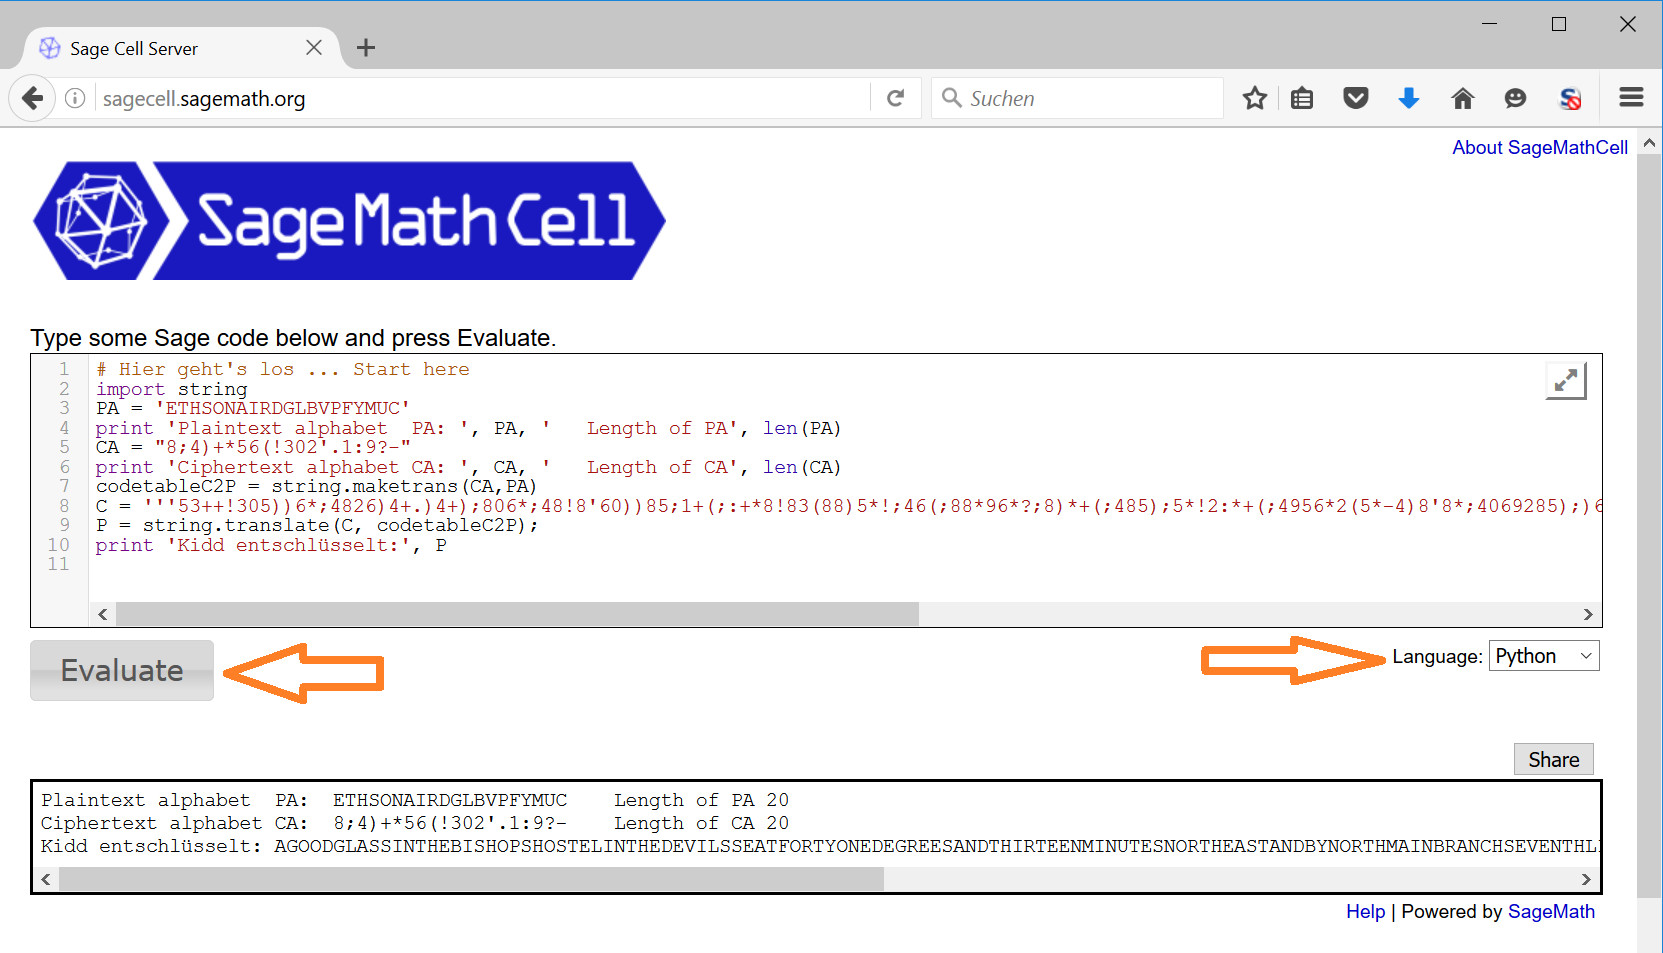
\includegraphics[scale=0.53]{../en/figures/Using-SageMathCell-with-Python-for-Poes-GoldBug}
\caption{Benutzung von SageMathCell, um Poes Goldkäfer zu entschlüsseln (mit Python\index{Python})}
\label{MOV_Using-SageMathCell-with-Python-for-Poes-GoldBug}
\end{center}
\end{figure}


\noindent Als Ergebnis erhalten wir:

% \noindent \verb muss auf derselben Zeile enden.
\begin{Verbatim}%

Plaintext alphabet  PA:  ETHSONAIRDGLBVPFYMUC    Length of PA 20
Ciphertext alphabet CA:  8;4)+*56(!302'.1:9?-    Length of CA 20
Kidd decrypted: AGOODGLASSINTHEBISHOPSHOSTELINTHEDEVILSSEATFORTYONEDEGREES
                ANDTHIRTEENMINUTESNORTHEASTANDBYNORTHMAINBRANCHSEVENTHLIMB
                EASTSIDESHOOTFROMTHELEFTEYEOFTHEDEATHSHEADABEELINEFROMTHE
                TREETHROUGHTHESHOTFIFTYFEETOUT

\end{Verbatim}

\noindent Man sieht gut, wie wenig Code man mit Python\index{Python} oder Sage für solche Aufgaben benötigt.
Im obigen Beispiel waren es 2 überflüssige Kommentarzeilen, 3 Zeilen Eingabe, 3 Zeilen echter Code und 3 Zeilen Ausgabe;
effektiv nötig waren 7 Zeilen Code.





% ++++++++++++++++++++++++++++++++++++++++++++++++++++++++++++++++++++++++++
\newpage
\hypertarget{appendix-Learn-NT}{}
\section{Lernprogramm Elementare Zahlentheorie}
    \label{s:appendix-Learn-NT}
    \index{ZT, Lernprogramm Zahlentheorie}%
    \index{Lernprogramm ZT}%

In CT1\index{CT1} ist ein interaktives Lernprogramm zur elementaren
{\em Zahlentheorie}, genannt "`ZT"', enthalten.\footnote{%
    ZT können Sie in CT1\index{CT1} über das Menü
    {\bf Einzelverfahren \textbackslash{} Zahlentheorie
    interaktiv \textbackslash{} Lernprogramm für Zahlentheorie} aufrufen.
}

Das Lernprogramm "`NT"' (Zahlentheorie) von Martin Ramberger führt in die
Zahlentheorie ein und visualisiert viele der Verfahren und Konzepte.
Wo nötig zeigt es auch die entsprechenden mathematischen Formeln.
Oftmals können die mathematischen Verfahren dynamisch mit eigenen kleinen
Zahlenbeispielen ausprobiert werden.

Die Inhalte basieren vor allem auf den Büchern von
\cite{Buchmann2016} und \cite{Scheid2006}.

Dieses visualisierte Lernprogramm wurde mit Authorware 4 erstellt.\footnote{%
    Da Authorware veraltet ist und der Hersteller keine Portierungswerkzeuge
    auf seine Nachfolgeprodukte zur Verfügung stellte, wird das ZT-Programm
    nicht mehr weiter entwickelt.
}

\paragraph*{Bitte um Erweiterung/Upgrade:}
Ein Update auf die neueste Version von Authorware oder auf eine andere
Entwicklungsplattform wäre wünschenswert. Wenn sich hierzu Interessenten
finden, würde ich mich sehr freuen (bitte E-Mail an den Autor des
CrypTool-Skriptes).


\paragraph*{Abbildungen:}
Die Abbildungen~\ref{NT_Fig_C1.3_EuclidsAlg-LinearCombinations}
bis~\ref{NT_Fig_C5.3_PollardRho} vermitteln einen Eindruck des
Lernprogramms "`ZT"':


% -> Figur 1  WIE ERREICHT MAN, dass er von vorne zählt ? (nicht wichtig)
%
% \includegraphics[scale=0.5]{figures/NT_Fig_C1.3_EuclidsAlg-LinearCombinations}
%    geht nicht. Im Dateinamen darf keine Punkt sein !!!?????!!!!!
%    Die Dateiendung muss man weglassen.
%
\begin{figure}[ht]
\begin{center}
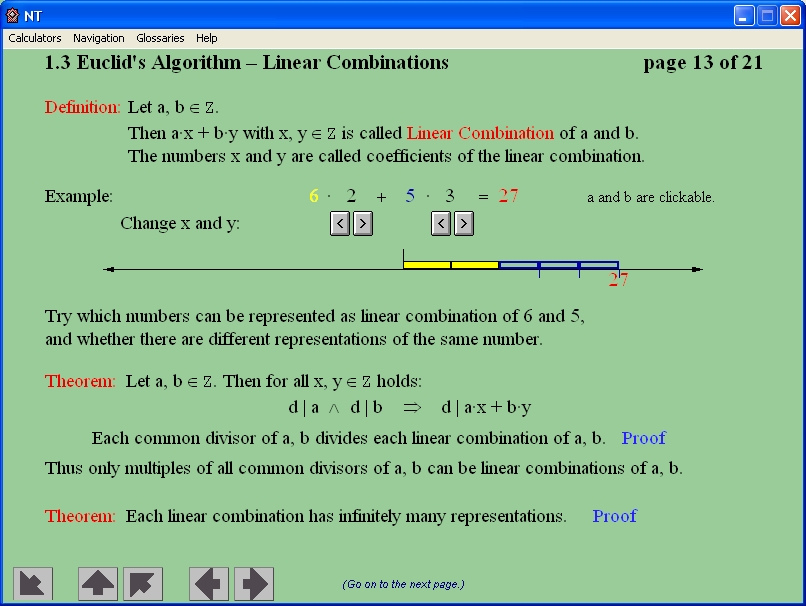
\includegraphics[scale=0.4]{figures/NT_Fig_C1-3_EuclidsAlg-LinearCombinations}
\caption{Jeder gemeinsame Teiler zweier Zahlen teilt auch alle ihre Linearkombinationen}
%%% TODO_Layout: Nur in Teilen von movies wird bei caption noch \vspace{1ex} hinzugefügt.
%%%              Damit sind die Abstände im Abbildungsverzeichnis von A.9 bis A.16
%%%              unterschiedlich vom Rest --> nahm es wieder raus. Analog wurde etwas
%%%              Platz unter den Abb-Untertitel in Kap. 7 geschaffen, der nun auch weg (22.8.16)
%%%              --> Wenn man es macht, dann muss man es überall machen!
%%% Bsp: vorher:  \caption{Euklids Algorithmus zur Bestimmung des ggT\vspace{1ex}}
%%%      nachher: \caption{Euklids Algorithmus zur Bestimmung des ggT}
\label{NT_Fig_C1.3_EuclidsAlg-LinearCombinations}
\end{center}
\end{figure}


\begin{figure}[ht]
\begin{center}
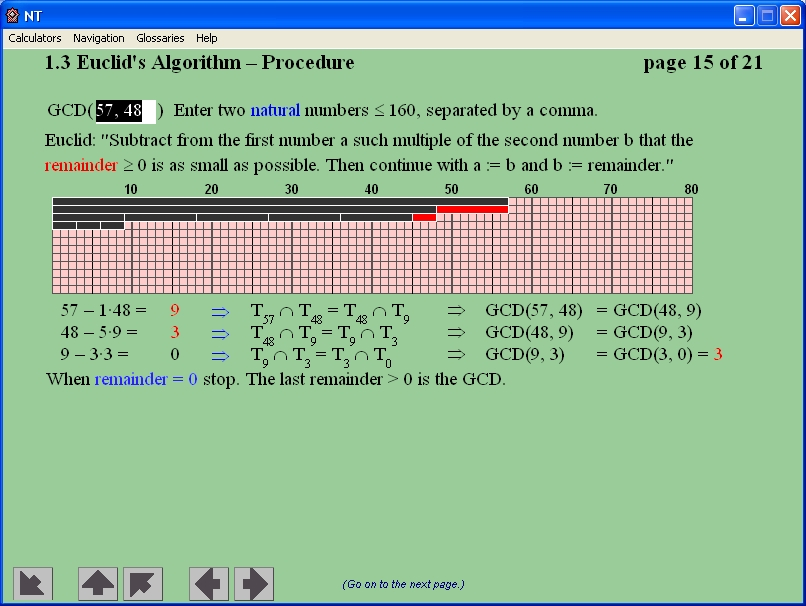
\includegraphics[scale=0.4]{figures/NT_Fig_C1-3_EuclidsAlg-Procedure}
\caption{Euklids Algorithmus zur Bestimmung des ggT}
\label{NT_Fig_C1.3_EuclidsAlg-Procedure}
\end{center}
\end{figure}


\begin{figure}[ht]
\begin{center}
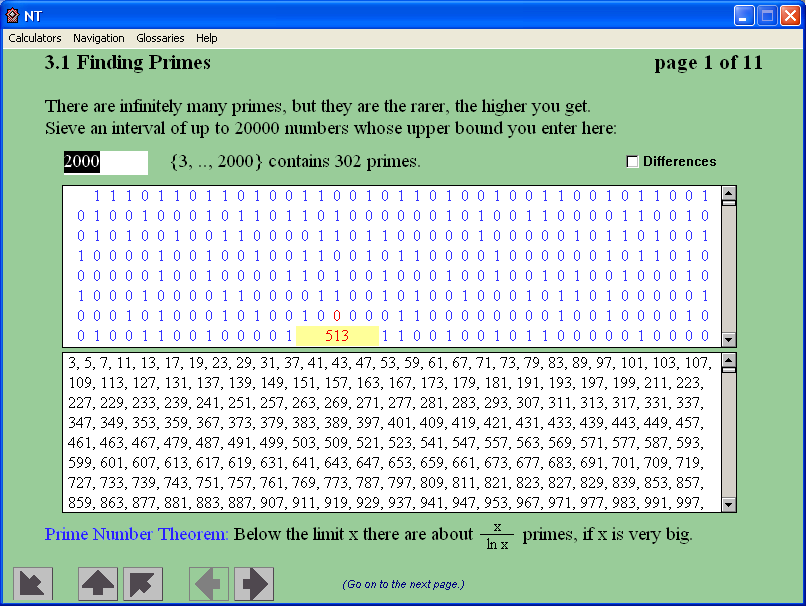
\includegraphics[scale=0.4]{figures/NT_Fig_C3-1_PrimesDistribution}
\caption{Verteilung der Primzahlen und ihrer Differenzen}
\label{NT_Fig_C3.1_PrimesDistribution}
\end{center}
\end{figure}


\begin{figure}[ht]
\begin{center}
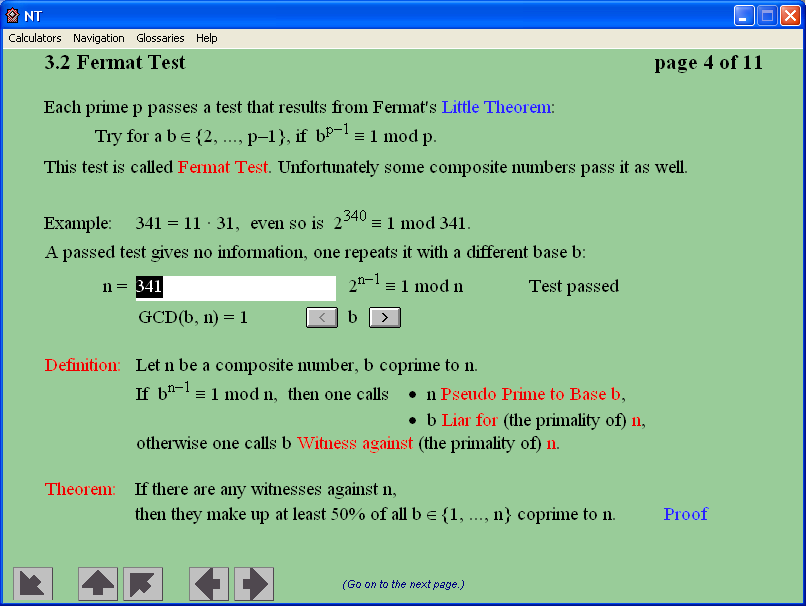
\includegraphics[scale=0.4]{figures/NT_Fig_C3-2_Fermat-Test}
\caption{Primzahlen finden mit dem Primzahltest nach Fermat}
\label{NT_Fig_C3.2_Fermat-Test}
\end{center}
\end{figure}


\begin{figure}[ht]
\begin{center}
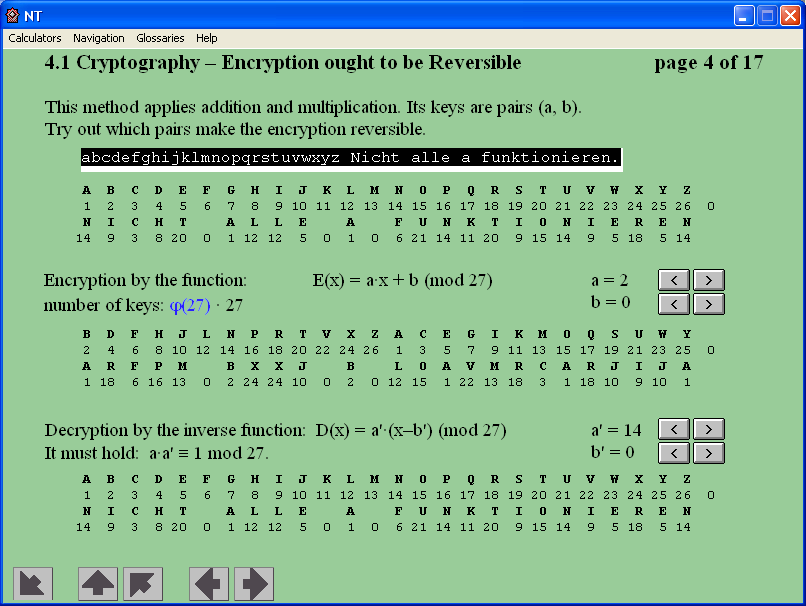
\includegraphics[scale=0.4]{figures/NT_Fig_C4-1_ReversibilityAdditiveCipher}
\caption{Umkehrbarkeit von Verschlüsselungsalgoritmen am Beispiel additiver Chiffren}
\label{NT_Fig_C4.1_ReversibilityAdditiveCipher}
\end{center}
\end{figure}


\begin{figure}[ht]
\begin{center}
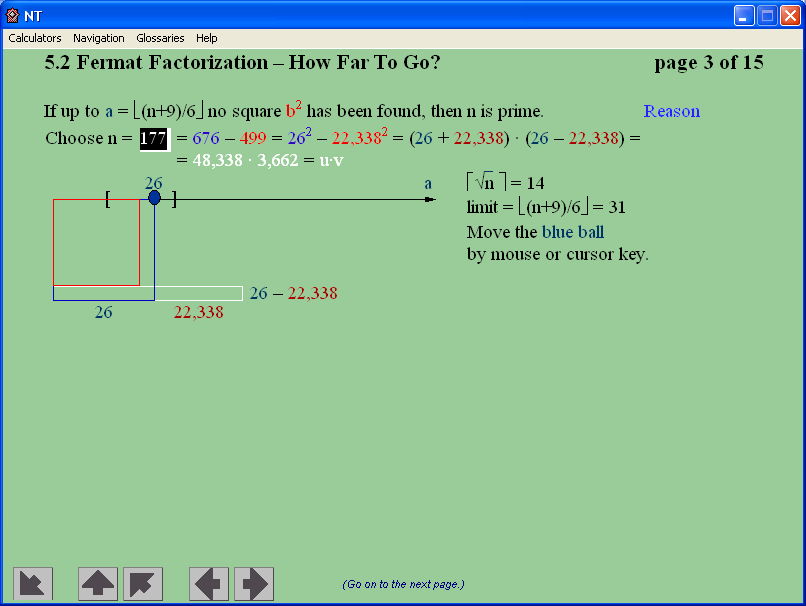
\includegraphics[scale=0.4]{figures/NT_Fig_C5-2_Fermat-factorization-How-far-1}
\caption{Fermat-Faktorisierung m.H. der 3. Binomischen Formel}
\label{NT_Fig_C5.2_Fermat-factorization-How-far-1}
\end{center}
\end{figure}


\begin{figure}[ht]
\begin{center}
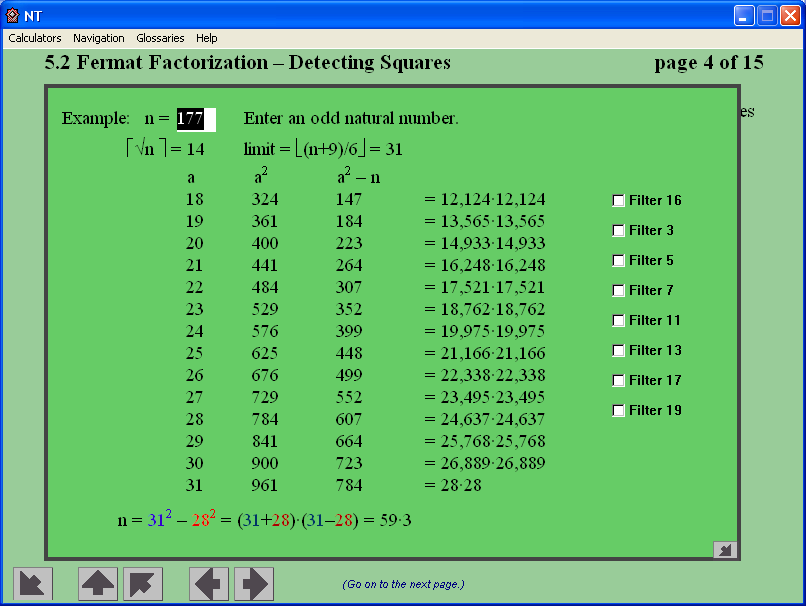
\includegraphics[scale=0.4]{figures/NT_Fig_C5-2_Fermat-factorization-How-far-2}
\caption{Fermat-Faktorisierung: Quadrate erkennen}
\label{NT_Fig_C5.2_Fermat-factorization-How-far-2}
\end{center}
\end{figure}


\begin{figure}[ht]
\begin{center}
\includegraphics[scale=0.4]{figures/NT_Fig_C5-3_PollardRho}
\caption{Pollards Rho-Faktorisierung: Kreisfindungsalgorithmus nach Floyd}
\label{NT_Fig_C5.3_PollardRho}
\end{center}
\end{figure}



%------------------------------------------------------------------------------
\printbibliography[%
	heading=subbibintoc,
	title={Literatur zu Kapitel \thechapter},
	segment=\therefsegment,
]


\end{refsegment}

  \renewcommand{\CTBChapName}{(Appendix Sage)}       % $Id:
% !Mode:: "TeX:DE"    % Setting document mode and submode for WinEdt
% ..............................................................................
%             W A S  I S T  S A G E M A T H  ?
% ~~~~~~~~~~~~~~~~~~~~~~~~~~~~~~~~~~~~~~~~~~~~~~~~~~~~~~~~~~~~~~~~~~~~~~~~~~~~~~

\newpage
\hypertarget{appendix-using-sage}{}
\section{Kurzeinführung in das CAS SageMath}
\label{s:appendix-using-sage}
\index{SageMath}
\index{SageMath!Programmbeispiele}

%% Unter \url{https://wiki.sagemath.org/combinat} gibt es Weiterentwicklung on-top of Sage.
%% Diese kommen meist nach und nach ins offizielle Sage rein.


Dieses Buch enthält zahlreiche mit SageMath erstellte Programmbeispiele. SageMath ist
ein Open-Source Computer-Algebra-System (CAS), das für Lehre, Studium und Forschung
eingesetzt wird.
SageMath kombiniert viele hochwertige Open-Source-Packete\footnote{%
Einen Eindruck von der Größe von SageMath erhält man, wenn man es selbst compiliert:
Die heruntergeladenen Sourcen von SageMath 4.1 brauchten zur Compilierung auf einem
durchschnittlichen Linux-PC rund 5 h (inklusive aller Bibliotheken).
Danach nahm es 1,8 GB Plattenplatz ein.
}
und liefert den Zugang zu deren Funktionalität über ein gemeinsames, auf der
Programmiersprache Python\index{Python} basierendes Interface\footnote{%
Es gibt auch ein relativ einfaches Interface für die Sprache C, genannt Cython,
mit der man eigene Funktionen in SageMath stark beschleunigen kann.\\
Siehe \url{http://openwetware.org/wiki/Open_writing_projects/Sage_and_cython_a_brief_introduction}.
}.

SageMath kann man auf vielfältige Weise nutzen:
als mächtigen Taschenrechner; als Tool für das Mathematikstudium;
oder als Programmier-Umgebung, um Algorithmen zu prototypen oder um Forschung im
Bereich der algorithmischen Aspekte der Mathematik zu betreiben.

Einen schnellen Einstieg bieten z.B. die Referenzen in dieser Fußnote%
\footnote{%
\begin{itemize}
\item[-] \glqq Einladung zu Sage\grqq~von David Joyner, letztes Update 2009,\\
  \url{http://sage.math.washington.edu/home/wdj/teaching/calc1-sage/an-invitation-to-sage.pdf}
\item[-]\glqq The SDSU Sage Tutorial\grqq,\\
  \url{http://www-rohan.sdsu.edu/~mosulliv/sagetutorial/}\\
  \url{http://www-rohan.sdsu.edu/~mosulliv/sagetutorial/sagecalc.html}
 \item[-]\glqq SAGE For Newbies\grqq~von Ted Kosan, 2007,\\
  \url{http://sage.math.washington.edu/home/tkosan/newbies_book/sage_for_newbies_v1.23.pdf} \end{itemize}}.

Die offizielle SageMath Online-Dokumentation\footnote{%
  Die entsprechenden offiziellen PDF-Dokuments können herunter geladen werden von\\
  \url{http://www.sagemath.org/help.html}, \url{http://www.sagemath.org/doc} und \url{http://planet.sagemath.org}.
} finden Sie unter: \url{http://www.sagemath.org}.


Es gibt inzwischen viele PDF- und HTML-Dokumente über SageMath, so dass wir als guten Startpunkt nur einige wenige nennen\footnote{%
- \glqq Bibliothek\grqq: {\centering \url{http://www.sagemath.org/library.html}},\\
- \glqq Dokumentationsprojekt\grqq:
  {\centering \url{http://wiki.sagemath.org/DocumentationProject}},\\
- \glqq Lehrmaterial\grqq: {\centering \url{http://wiki.sagemath.org/Teaching_with_SAGE}}.
}.

Auch beim Studium der Kryptologie können fertige SageMath-Module genutzt
werden\footnote{%
\begin{itemize}
\item[-]
Überblick,
   welche Kryptographie momentan in SageMath enthalten ist:\\
   \url{http://www.sagemath.org/doc/reference/sage/crypto/}
\item[-]Diskussionen
   über Lernaspekte beim Entwickeln weiterer Krypto-Module in SageMath:\\
   \url{http://groups.google.com/group/sage-devel/browse_thread/thread/c5572c4d8d42d081}
\end{itemize}
}.

Umfangreiche Kryptographie-Einführungen finden sich in der folgenden Fußnote\footnote{%
\begin{itemize}
\item[-]
Ein fertiger Kryptographie-Kurs von David Kohel,
  der SageMath nutzt, aus 2008:\\
  \url{http://www.sagemath.org/files/kohel-book-2008.pdf}\\
  bzw. derselbe Kurs in einer neueren Fassung (2015)\\
  \url{http://iml.univ-mrs.fr/~kohel/tch/M2-CryptoSymetrique/crypto.pdf}
\item[-]\glqq Introduction to Cryptography with
  Open-Source Software\grqq, ein hervorragendes Buch von Alasdair McAndrew, CRC, 2011
\end{itemize}
}.


% ---------------------------------------------------------------------------
\section*{SageMath-Benutzerschnittstellen}
SageMath ist kostenlos und kann von folgender Webseite herunter geladen werden:
\begin{center}
  \url{http://www.sagemath.org} \\
\end{center}
Standardmäßig nutzt man die SageMath-\textbf{Kommandozeile} als Interface, wie im
folgenden Bild~\ref{fig:sage_cmd_interfaces} zu sehen ist.
Es gibt jedoch auch ein grafisches Benutzerinterface für diese Software
in Form des SageMath-Notebooks (siehe Bild~\ref{fig:sage_gui_interfaces}).
Und schließlich kann man SageMath-\textbf{Notebooks}\footnote{%
Weitere Details zu SageMath-Notebooks finden Sie in
Kapitel~\ref{ec:Sage_Massierer}
(\glqq \nameref{ec:Implementing-for-Education}\grqq
  $\Rightarrow$ \glqq \nameref{ec:Sage_Massierer}\grqq).
                      }
auch online auf verschiedenen Servern nutzen, ohne SageMath lokal zu installieren, z.B.:
\begin{center}
\url{http://sagecell.sagemath.org/} oder \\
\url{https://cocalc.com/}
\end{center}

SageMath läuft unter den Betriebssystemen Linux, Mac OS X und Windows.
Auf der Windows-Plattform läuft die komplette SageMath-Distribution momentan
nur als ein VMware-Image.

\begin{figure}[!htpb]
\centering
\includegraphics[scale=0.6]{figures/sage-cmd}
\caption{SageMath-Kommandozeilen-Interface}
\label{fig:sage_cmd_interfaces}
\end{figure}

\begin{figure}[!htpb]
\centering
\includegraphics[scale=0.4]{figures/sage-gui}
\caption[SageMath-Notebook-Interface]{SageMath-Notebook-Interface\footnotemark}
\label{fig:sage_gui_interfaces}
\end{figure}

\footnotetext{%
Um das grafische SageMath-Interface lokal zu starten, muss man auf der SageMath-Kommandozeile
\verb#notebook()# eingeben. Danach startet der eingestellte Browser (Iceweasel,
Firefox, IE, ...) z.B. mit der URL \textit{http://localhost:8000}.
}



% ---------------------------------------------------------------------------
\newpage
\section*{Hilfe beim Benutzen von SageMath}

Wenn man SageMath auf der Kommandozeile startet, erhält etwas wie die folgenden Zeilen:
%
\begin{Verbatim}%
[fontsize=\footnotesize]
mnemonic:~$ sage
----------------------------------------------------------------------
| Sage Version 4.1, Release Date: 2009-07-09                         |
| Type notebook() for the GUI, and license() for information.        |
----------------------------------------------------------------------

sage: help
Type help() for interactive help, or help(object) for help about object.
sage:
sage:
sage: help()

Welcome to Python 2.6!  This is the online help utility.

If this is your first time using Python, you should definitely check out
the tutorial on the Internet at http://docs.python.org/tutorial/.

Enter the name of any module, keyword, or topic to get help on writing
Python programs and using Python modules.  To quit this help utility and
return to the interpreter, just type "quit".

To get a list of available modules, keywords, or topics, type "modules",
"keywords", or "topics".  Each module also comes with a one-line summary
of what it does; to list the modules whose summaries contain a given word
such as "spam", type "modules spam".
\end{Verbatim}
%
Viele weitere Hilfen gibt es als offizielle SageMath-Dokumentation, die mit jedem
Release von SageMath verteilt wird~(siehe Bild~\ref{fig:sage_standard_doc}).
%
\begin{figure}[!htpb]
\centering
\includegraphics[scale=0.4]{figures/sage-online-doc}
\caption{Die Standard-Dokumentation von SageMath}
\label{fig:sage_standard_doc}
\end{figure}
%
Zur offiziellen SageMath-Standard-Dokumentation gehören folgende Dokumente:

\begin{itemize}
\item Tutorial --- Das Tutorial ist für SageMath-Einsteiger.
  Es ist dafür gedacht, sich in ein bis drei Stunden mit den
  wichtigsten Funktionen vertraut zu machen.

\item Constructions --- Dieses Dokument ist im Stil eines \glqq Kochbuchs\grqq~mit
  einer Sammlung von Antworten auf Fragen zur Konstruktion von SageMath-Objekten.

\item Developers' Guide --- Dieser Führer ist für Entwickler, die selbst SageMath
  mit weiter entwickeln wollen. Enthalten sind darin z.B. Hinweise zum
  Stil und zu Konventionen beim Programmieren, zur Modifikation von
  SageMath-Kern-Bibliotheken oder von SageMath-Standard-Dokumentation, und zum Code-Review
  und zur Software-Verteilung.

\item Reference Manual --- Dieses Handbuch enthält die komplette Dokumentation
  aller wichtigen SageMath-Funktionen. Zu jeder Klassen-Beschreibung gibt es
  mehrere Code-Beispiele. Alle Code-Beispiele im Referenz-Handbuch werden
  bei jedem neuen SageMath-Release getestet.

\item Installation Guide --- Dieser Führer erklärt, wie man SageMath auf
  verschiedenen Plattformen installiert.

\item A Tour of Sage --- Diese Tour durch SageMath zeigt exemplarisch verschiedene
  Funktionen, die für Einsteiger sinnvoll sind.

\item Numerical Sage --- Dieses Dokument führt Werkzeuge auf, die in SageMath
  für numerische Mathematik verfügbar sind.

\item Three Lectures about Explicit Methods in Number Theory Using
  Sage --- Drei Vorlesungen über Methoden der Zahlentheorie, die explizit
  SageMath nutzen. Dieses Dokument zeigt wie man mit SageMath Berechnungen in
  fortgeschrittener Zahlentheorie durchführt.
\end{itemize}

Von der SageMath-Kommandozeile erhält man eine Liste aller verfügbaren Kommandos
(Funktionsnamen etc.), die ein bestimmtes Muster haben, wenn man die ersten Zeichen tippt,
und dann die \glqq Tab\grqq-Taste drückt:
%
\begin{Verbatim}%
[fontsize=\footnotesize]
sage: Su[TAB]
Subsets                   Subwords                  SuzukiGroup
SubstitutionCryptosystem  SupersingularModule
\end{Verbatim}
%
Wenn man den genauen Namen eines Kommandos kennt, kann man die \texttt{help}-Funktion
nutzen oder das Fragezeichen \glqq ?\grqq~anfügen, um weitere Informationen zu
diesem Kommando zu erhalten.  Zum Beispiel liefert das Kommando
\texttt{help(SubstitutionCryptosystem)} die Dokumentation zur der eingebauten
Klasse \texttt{SubstitutionCryptosystem}. Mit dem Fragezeichen erhalten wir die
Dokumentation zu dieser Klasse auf folgende Weise:
%
\begin{Verbatim}%
[fontsize=\footnotesize]
sage: SubstitutionCryptosystem?
Type:type
Base Class:<type 'type'>
String Form:<class 'sage.crypto.classical.SubstitutionCryptosystem'>
Namespace:Interactive
File:/home/mvngu/usr/bin/sage-3.4.1/local/lib/python2.5/site-packages/sage/crypto/classical.py
Docstring:

        Create a substitution cryptosystem.

        INPUT:

        - ``S`` - a string monoid over some alphabet

        OUTPUT:

        - A substitution cryptosystem over the alphabet ``S``.

        EXAMPLES::

            sage: M = AlphabeticStrings()
            sage: E = SubstitutionCryptosystem(M)
            sage: E
            Substitution cryptosystem on Free alphabetic string monoid
            on A-Z
            sage: K = M([ 25-i for i in range(26) ])
            sage: K
            ZYXWVUTSRQPONMLKJIHGFEDCBA
            sage: e = E(K)
            sage: m = M(``THECATINTHEHAT'')
            sage: e(m)
            GSVXZGRMGSVSZG

        TESTS::

            sage: M = AlphabeticStrings()
            sage: E = SubstitutionCryptosystem(M)
            sage: E == loads(dumps(E))
            True
\end{Verbatim}
%
\vspace{30pt}
Weitere Unterstützung für spezifische Probleme gibt es in den Archiven der
\texttt{sage-support} Mailing-Liste unter
%
\begin{center}
  \url{http://groups.google.com/group/sage-support}
\end{center}




% ---------------------------------------------------------------------------
\newpage
\section*{Beispiele für in SageMath eingebaute mathematische Funktionen}

Hier sind ein paar kleine Beispiele\footnote{%
Diese Beispiele stammen aus einem nicht mehr existierenden Blog aus 2008 von Dr. Alasdair McAndrew.
%%%, Victoria University
%%%,\\ \url{http://amca01.wordpress.com/2008/12/19/sage-an-open-source-mathematics-software-system}
}
(alle für das Kommandozeilen-Interface -- zur einfacheren Nutzung), um zu sehen,
was man mit SageMath machen kann:

\begin{sagecode}
\begin{Verbatim}%
[fontsize=\footnotesize]
# * Analysis (Infinitesimalrechnung):
    sage: x=var('x')
    sage: p=diff(exp(x^2),x,10)*exp(-x^2)
    sage: p.simplify_exp()
     1024 x^10 + 23040 x^8 + 161280 x^6 + 403200 x^4 + 302400 x^2 + 30240

# * Lineare Algebra:
    sage: M=matrix([[1,2,3],[4,5,6],[7,8,10]])
    sage: c=random_matrix(ZZ,3,1);c
     [ 7 ]
     [-2 ]
     [-2 ]
    sage: b=M*c
    sage: M^-1*b
     [ 7 ]
     [-2 ]
     [-2 ]

# * Zahlentheorie:
    sage: p=next_prime(randint(2^49,2^50));p
      1022095718672689
    sage: r=primitive_root(p);r
      7
    sage: pl=log(mod(10^15,p),r);pl
      1004868498084144
    sage: mod(r,p)^pl
      1000000000000000

# * Endliche Körper (\url{http://de.wikipedia.org/wiki/Endlicher_K%C3%B6rper}):
    sage: F.<x>=GF(2)[]
    sage: G.<a>=GF(2^4,name='a',modulus=x^4+x+1)
    sage: a^2/(a^2+1)
      a^3 + a
    sage: a^100
      a^2 + a + 1
    sage: log(a^2,a^3+1)
      13
    sage: (a^3+1)^13
      a^2
\end{Verbatim}
\caption{Einige kleine Beispiele in SageMath aus verschiedenen Gebieten der Mathematik}
\end{sagecode}



% ---------------------------------------------------------------------------
\newpage
\section*{Programmieren mit SageMath}

Wenn man ein CAS (Computer-Algebra-System) nutzt, schreibt man zu Beginn einzelne
Befehle in die Kommandozeile wie im obigen Beispiel\footnote{%
  Standardmäßig wird SageMath-Code auch so präsentiert: Dabei beginnen die Zeilen
  mit  \glqq sage:\grqq~und \glqq ...\grqq.
  \begin{Verbatim}%
  [fontsize=\footnotesize]
  sage: m = 11
  sage: for a in xrange(1, m):
  ....:     print [power_mod(a, i, m) for i in xrange(1, m)]
  ....:
  \end{Verbatim}

  Auch dieses Skript benutzt normalerweise die obige Konvention, um
  SageMath-Code zu präsentieren, solange der Code nicht aus einer SageMath-Skriptdatei kommt.
  Wenn man den SageMath-Code aus diesem Skript kopiert und per Paste auf der SageMath-Kommandozeile
  wieder einfügt, sollte man \glqq sage:\grqq~und \glqq ...\grqq~ weglassen
  (obwohl das Kommandozeilen-Interface in den meisten Fällen mit diesen Präfixen
  korrekt umgehen kann).}.

Wenn man eigene Funktionen entwickelt, sie ändert und aufruft, dann ist es viel einfacher,
die Entwicklung in einem eigenen Editor vorzunehmen, den Code als SageMath-Skriptdatei zu
speichern und die Funktionen nicht-interaktiv auf der Kommandozeile auszuführen.
Beide Arten, Code zu entwickeln, wurden in
Kapitel \ref{CM_Sage_samples} (\glqq \nameref{CM_Sage_samples}\grqq),
Kapitel \ref{PaP_Sage_samples} (\glqq \nameref{PaP_Sage_samples}\grqq),
Kapitel \ref{primes:_Appendix_Sage-Samples} (\glqq \nameref{primes:_Appendix_Sage-Samples}\grqq)
und in Kapitel \ref{NumberTheory_Appendix_E} (\glqq\nameref{NumberTheory_Appendix_E}\grqq)
angewandt.

Um SageMath-Code in einem eigenen Editor zu entwickeln und zu testen, gibt es zwei
nützliche Befehle: \verb!load()! und \verb!attach()!\footnote{%
Vergleiche das SageMath-Tutorial über Programmierung, Kapitel
\glqq Loading and Attaching Sage files\grqq,\\
\url{http://doc.sagemath.org/html/en/tutorial/programming.html}.}.\\
Angenommen Sie haben die folgende Funktions-Definition:
\begin{Verbatim}%
   [fontsize=\footnotesize]
   def function(var1):
       r"""
       DocText.
       """
       ...
       return (L)
\end{Verbatim}
die in der Datei \texttt{primroots.sage} gespeichert wurde.

Um diese Funktion in SageMath zu laden (und syntaktisch gleich zu testen),
wird der Befehl \verb!load()! benutzt:

\texttt{sage: load primroots.sage}

Danach kann man auf der Kommandozeile alle Variablen und Funktionen
nutzen, die im Sage\-Math-Skript definiert wurden\footnote{%
Anmerkungen:
\begin{itemize}
\item[-]
Bitte keine Leerzeichen
oder White Spaces im Dateinamen.
\item[-]Es empfiehlt sich,
der SageMath-Skriptdatei die Datei-Extension
\glqq .sage\grqq~statt \glqq .py\grqq~zu geben.
Hat ein SageMath-Skript die Dateinamens-Endung \glqq .sage\grqq, dann wird
beim Laden der Datei in SageMath auch gleich die normale SageMath-Umgebung mit geladen,
um die Syntax zu prüfen. Genauso funktioniert es, wenn man ein SageMath-Skript direkt
von einer Bash-Shell aufruft mit~~\texttt{\$ sage primroots.sage}.
\item[-]Beim Laden des obigen
SageMath-Skripts wird es von SageMath zuerst geparst, und dann
in eine andere Datei namens \glqq primroots.py\grqq~kopiert. SageMath ergänzt
dann alle notwendigen Variablen in \glqq primroots.py\grqq~und alle Import-Statements.
Somit wird das SageMath-Skript genauso ausgeführt, als hätte man die Befehle einzeln
auf der Kommandozeile eingetippt. Ein bedeutender Unterschied ist,
dass alle Ausgaben ein \verb!print!~benötigen.
\end{itemize}
}.

Normalerweise editiert man ein eigenes SageMath-Skript wieder und möchte dann den
Inhalt des geänderten Skripts wieder in SageMath laden. Dafür kann man den Befehl
\verb!attach()! nutzen (man kann auch direkt nach dem \verb!load()!
das \verb!attach()! aufrufen, und nicht erst, wenn man das Skript ändert;
man kann \verb!load()! sogar weglassen, da dies in \verb!attach()! enthalten ist):

\texttt{sage: attach primroots.sage}

Nun kann man das SageMath-Skript ändern und die geänderte Funktionsdefinition
wird -- solange man die SageMath-Session nicht beendet -- beim nächsten Enter
in SageMath geladen (und syntaktisch gleich geprüft). Diese Neuladen passiert
vollkommen automatisch. Der Befehl attach() lässt SageMath also permanent die
genannte Datei auf Änderungen überwachen. Damit spart man sich das Kopieren
und Pasten zwischen dem eigenen Texteditor und dem SageMath-Kommandozeilen-Interface.

Hier ist ein Bild, das SageMath-Code im Editor GVIM zeigt -- mit aktiviertem
Syntax-Highlighting (siehe Bild~\ref{fig:sage-highlighted-code-in-editor}).
%
\begin{figure}[!htpb]
\centering
\includegraphics[scale=0.7]{figures/sage-highlighted-code-in-editor}
\caption{SageMath-Beispiel in einem Editor mit aktiviertem Code-Highlighting}
\label{fig:sage-highlighted-code-in-editor}
\end{figure}

\vspace{20pt}
Falls man die Ausgabe einer attachten Datei so angezeigt haben möchte,
wie wenn man die Einzelbefehle direkt auf der Kommandozeile eingibt
(also nicht nur das, was per \verb!print! ausgegeben wird),
kann man den Befehl \verb!iload()! verwenden:
Jede Zeile wird dann einzeln geladen. Um die nächste Zeile zu laden,
muss man die \verb!Enter!-Taste drücken. Das muss man so lange wiederholen,
bis alle Zeilen des SageMath-Skripts in die SageMath-Session geladen sind.

\texttt{sage: iload primroots.sage}


% \vspace{30pt}
\newpage
Weitere Hinweise:
\begin{itemize}
  \item Abfrage der Version Ihrer SageMath-Umgebung mit: \texttt{version()}
  \item Um sich schnell die SageMath-Programmbeispiele in diesem Skript anzusehen, können Sie
    \begin{itemize}
      \item im Index nach \verb#SageMath -> Programmbeispiele# schauen, oder
      \item sich im Anhang das \glqq \nameref{sc:List-of-Sage-Code-Examples}\grqq~ansehen.
    \end{itemize}
  \item Die SageMath-Beispiele in diesem Skript werden mit CrypTool ausgeliefert.\\
        Weitere Details am Ende der Übersicht
        \glqq \nameref{sc:List-of-Sage-Code-Examples}\grqq.
\end{itemize}



  \renewcommand{\CTBChapName}{(Appendix Authors)}    
% ++++++++++++++++++++++++++++++++++++++++++++++++++++++++++++++++++++++++++
\hypertarget{appendix-authors}{}
\section{Autoren des CrypTool-Skripts}\index{CrypTool}
\label{s:appendix-authors}

Dieser Anhang f�hrt die Autoren\index{Autoren} dieses Dokuments auf.\\
Die Autoren sind namentlich am Anfang jedes Kapitels aufgef�hrt,
zu dem sie beigetragen haben.

\begin{description}

\item[Bernhard Esslinger,] \mbox{}\\  % be_2005: Das \\ allein wird ignoriert (brauche beide)!  
Initiator des CrypTool-Projekts, Hauptautor dieses Skripts, Leiter IT-Security
in der Deutschen Bank und Professor an der Universit�t Siegen. \\
E-Mail: esslinger@fb5.uni-siegen.de.

---------

\item[Matthias B�ger,] \mbox{}\\
Mitautor des Kapitels ``Elliptische Kurven'',
Research Analyst bei der Deutschen Bank.

\item[Bartol Filipovic,] \mbox{}\\
Urspr�nglicher Autor der Elliptische-Kurven-Implementierung
in CrypTool und des entsprechenden Kapitels in diesem Skript.

\item[Henrik Koy, ] \mbox{}\\
Hauptentwickler und Koordinator der CrypTool-Entwicklung
seit Version 1.3, Reviewer des Skripts und \TeX{}-Guru, 
Projektleiter IT und Kryptologe bei der Deutschen Bank.

\item[Roger Oyono, ] \mbox{}\\
Implementierer des Faktorisierungs-Dialogs in CrypTool und urspr�nglicher
Autor des Kapitels "`Die mathematischen Ideen hinter der modernen
Kryptographie"'.

\item[J�rg Cornelius Schneider,] \mbox{}\\
Design und Support von CrypTool, Kryptographie-Enthusiast und IT-Architekt und 
Seni"-or-Projektleiter IT bei der Deutschen Bank.

\item[Christine St�tzel,] \mbox{}\\
Diplom Wirtschaftsinformatikerin an der Universit�t Siegen.

---------

\item[Johannes Buchmann,] \mbox{}\\
Mitautor des Kapitels ``Krypto 2020 --- Perspektiven f�r langfristige
kryptographische Sicherheit'', 
Vizepr�sident der TU Darmstadt (TUD) und Professor an den Fachbereichen
f�r Informatik und Mathematik der TUD.  Dort hat er den Lehrstuhl
f�r Theoretische Informatik (Kryptographie und Computer-Algebra).

\item[Alexander May,] \mbox{}\\
Mitautor des Kapitels ``Krypto 2020 --- Perspektiven f�r langfristige
kryptographische Sicherheit'', 
Junior-Professor am Fachbereich Informatik der TU Darmstadt.

\item[Erik Dahmen,] \mbox{}\\
Mitautor des Kapitels ``Krypto 2020 --- Perspektiven f�r langfristige
kryptographische Sicherheit'', 
Mitarbeiter am Lehrstuhl Theoretische Informatik (Kryptographie und
Computeralgebra) der TU Darmstadt.

\item[Ulrich Vollmer,] \mbox{}\\
Mitautor des Kapitels ``Krypto 2020 --- Perspektiven f�r langfristige
kryptographische Sicherheit'', 
Mitarbeiter am Lehrstuhl Theoretische Informatik (Kryptographie und
Computeralgebra) der TU Darmstadt.

---------

\item[Minh Van Nguyen,] \mbox{}\\
Sage-Entwickler und Reviewer des Dokuments.


\end{description}






% ++++++++++++++++++++++++++++++++++++++++++++++++++++++++++++++++++++++++++
\newpage
\hypertarget{appendix-movies}{}
\section{Filme und belletristische Literatur mit Bezug zur Kryptographie,
Kinderb�cher mit einfachen Verschl�sselungen}
\label{s:appendix-movies}  
% {\bf Filme und Literatur mit Bezug zur Kryptographie} (siehe Anhang \ref{s:appendix-movies})
\index{Filme}
\index{Literatur}


Kryptographische Verfahren -- sowohl klassische wie moderne -- fanden auch
Eingang in die Literatur und in Filme. In manchen Medien werden diese nur
erw�hnt und sind reine Beigabe, in anderen sind sie tragend und werden
genau erl�utert, und manchmal ist die Rahmenhandlung nur dazu da, dieses
Wissen motivierend zu transportieren. Anbei der Beginn eines �berblicks.

\subsection{F�r Erwachsene}

%be_2005: Hatte zuerst \begin{thebibliography}{99999} und \bibitem[... ,
%         aber dann wurde immer der feste Titel "Literatur" bzw. "References"
%         geschrieben und wir fanden keine M�glichkeit, ihn weg zu bekommen.
%         L�sung: Stattdessen \begin{description} \item[...


\begin{description}

\item[\textrm{[Poe1843]}] \index{Poe 1843}
    Edgar Allan Poe\index{Poe, Edgar Allan}, \\
    {\em Der Goldk�fer}, 1843. \\
    Diese Kurzgeschichte erschien in Deutsch z.B. in der illustrierten und
    mit Kommentaren in den Marginalspalten versehenen Ausgabe "`Der Goldk�fer
    und andere Erz�hlungen"', Gerstenbergs visuelle Weltliteratur,
    Gerstenberg Verlag, Hildesheim, 2002.\\
    In dieser Kurzgeschichte beschreibt Poe als Ich-Erz�hler seine
    Bekanntschaft mit dem sonderbaren Legrand. Mit Hilfe eines an der
    K�ste Neuenglands gefundenen Goldk�fers, einem alten Pergament und
    den Dechiffrierk�nsten von Legrand finden Sie den sagenhaften Schatz
    von Kapit�n Kidd.\\
    Die Geheimschrift besteht aus 203 kryptischen Zeichen und erweist sich
    als allgemeine monoalphabetische Substitutions-Chiffre (vgl. 
    Kapitel~\ref{monoalphabeticSubstitutionCiphers}). Ihre schrittweise 
    Dechiffrierung durch semantische und syntaktische Analyse
    (H�ufigkeiten der einzelnen Buchstaben in englischen Texten)
    wird ausf�hrlich erl�utert.\\
    Der Entschl�sseler Legrand sagt darin (S. 39) den ber�hmten Satz:
    "`Und es ist wohl sehr zu bezweifeln, ob menschlicher Scharfsinn
    ein R�tsel ersinnen kann, das menschlicher Scharfsinn bei
    entsprechender Hingabe nicht wieder zu l�sen vermag."'\\
    % D: Poe: 1809-1849, "Vater des Kriminalromans", er schloss Wetten ab,
    % dass er alle verschl�sselten Botschaften, die ihm Freunde und Leser
    % vorlegten, im Handumdrehen entschl�sseln k�nne. Gutes Gesp�r durch
    % viel �bung.
    % E: Poe, 1809-1849 was named "Father of the crime novel". He claimed,
    % that he will be able to decrypt any cipher sent to him by friends or
    % readers.
 
    % Originalausgabe dieser illustrierten Ausgabe: "Le scarab�e d'or et 
    %                           autre nouvelles", Gallimard, Paris, 1998.
    % In "Der Goldk�fer" wird detailliert beschrieben, wie der verarmte
    % Hugenotte William Legrand in South Carolina die monoalphabetische
    % Geheimschrift des Piratenkapit�ns Kidd knackt, die zu einem
    % sagenhaften Schatz f�hrt.



\item[\textrm{[Verne1885]}] \index{Verne 1885}
    Jules Verne\index{Verne, Jules}, \\
    {\em Mathias Sandorf}, 1885. \\
    Dies ist einer der bekanntesten Romane des franz�sischen Schriftstellers
    Jules Verne (1828-1905), der auch als "`Vater der Science Fiction"'
    bezeichnet wurde.\\
    Erz�hlt wird die spannende Geschichte des Freiheitsk�mpfers Graf
    Sandorf, der an die Polizei verraten wird, aber schlie�lich fliehen
    kann.\\
    M�glich wurde der Verrat nur, weil seine Feinde eine Geheimbotschaft an
    ihn abfangen und entschl�sseln konnten. Dazu ben�tigten sie eine
    besondere Schablone, die sie ihm stahlen. Diese Schablone bestand aus
    einem quadratischen St�ck Karton mit 6x6 K�stchen, wovon 1/4, also neun,
    ausgeschnitten waren (vgl. die
    \hyperlink{turning-grille}{Flei�ner-Schablone}
    in Kapitel~\ref{introsamplesTranspositionCiphers}).\\


% Gefunden in: CRYPTO-GRAM, January 15, 2007, by Bruce Schneier
\item[\textrm{[Kipling1901]}] \index{Kipling 1901}
    Rudyard Kipling\index{Kipling, Rudyard}, \\
    {\em Kim}, 1901. \\
    Dieser Roman wird in der Besprechung von Rob Slade%
    \footnote{See
          \href{http://catless.ncl.ac.uk/Risks/24.49.html\#subj12} %% \ vor # n�tig !
       {\texttt{http://catless.ncl.ac.uk/Risks/24.49.html\#subj12}}.
    }
    folgenderma�en beschrieben:
    "`Kipling packte viele Informationen und Konzepte in seine Geschichten.
    In "`Kim"' geht es um das gro�e "`Spiel"' Spionage und Bespitzelung.
    Schon auf den ersten 20 Seite finden sich Authentisierung �ber Besitz,
    Denial of Service, Sich-f�r-jemand-anderen-Ausgeben (Impersonation),
    Heimlichkeit, Maskerade, Rollen-basierte Autorisierung (mit 
    Ad-hoc-Authentisierung durch Wissen), Abh�ren, und Vertrauen basierend
    auf Datenintegrit�t.
    Sp�ter kommen noch Contingency Planning gegen Diebstahl und
    Kryptographie mit Schl�sselwechsel hinzu."'\\
    Das Copyright des Buches ist abgelaufen%
    \footnote{Sie k�nnen es lesen unter:\\
          \href{http://whitewolf.newcastle.edu.au/words/authors/K/KiplingRudyard/prose/Kim/index.html}
       {\texttt{http://whitewolf.newcastle.edu.au/words/authors/K/KiplingRudyard/prose/Kim/index.html}},\\
          \href{http://kipling.thefreelibrary.com/Kim}
       {\texttt{http://kipling.thefreelibrary.com/Kim}} or\\
          \href{http://www.readprint.com/work-935/Rudyard-Kipling}
       {\texttt{http://www.readprint.com/work-935/Rudyard-Kipling}}.
    }.\\


\item[\textrm{[Doyle1905]}] \index{Doyle 1905}
    Arthur Conan Doyle\index{Doyle, Sir Arthur Conan}, \\
    {\em Die tanzenden M�nnchen}, 1905. \\
    In der Sherlock-Holmes-Erz�hlung {\em Die tanzenden M�nnchen} 
    (erschienen erstmals 1903 im "`Strand Magazine"', und dann 1905 im 
    Sammelband "`Die R�ckkehr des Sherlock Holmes"' erstmals in Buchform)
    wird Sherlock Holmes mit einer Geheimschrift konfrontiert, die zun�chst
    wie eine harmlose Kinderzeichnung aussieht. \\
    Sie erweist sich als monoalphabetische Substitutions-Chiffre (vgl. 
    Kapitel~\ref{monoalphabeticSubstitutionCiphers}) des Verbrechers Abe
    Slaney. Holmes knackt die Geheimschrift mittels H�ufigkeitsanaly"-se.\\


\item[\textrm{[Sayers1932]}] \index{Sayers 1932}
    Dorothy L. Sayers, \\
    {\em Zur fraglichen Stunde und Der Fund in den Teufelsklippen 
    (Orginaltitel: Have his carcase)}, Harper, 1932 \\
    (1. dt. �bersetzung {\em Mein Hobby: Mord} bei A. Scherz, 1964; \\
    dann {\em Der Fund in den Teufelsklippen} bei Rainer Wunderlich-Verlag, 
    1974;\\
    Neu�bersetzung 1980 im Rowohlt-Verlag). \\
    In diesem Roman findet die Schriftstellerin Harriet Vane eine Leiche 
    am Strand und die Polizei h�lt den Tod f�r einen Selbstmord. 
    Doch Harriet Vane und der elegante Amateurdetektiv Lord Peter Wimsey
    kl�ren in diesem zweiten von Sayers's ber�hmten Harriet Vane's
    Geschichten den widerlichen Mord auf. \\
    Dazu ist ein Chiffrat zu l�sen. Erstaunlicherweise beschreibt der
    Roman nicht nur detailliert die Playfair-Chiffre, sondern auch deren
    Kryptoanalyse (vgl. \hyperlink{playfair}{Playfair}
    in Kapitel~\ref{polygraphicSubstitutionCiphers}).\\


\item[\textrm{[Arthur196x]}] \index{Arthur 196x}
    Robert Arthur, \\
    {\em Die 3 ???: Der geheime Schl�ssel nach Alfred Hitchcock (Band 119)},
    Kosmos-Verlag (ab 1960) \\
    Darin m�ssen die drei Detektive Justus, Peter und Bob verdeckte und
    verschl�sselte Botschaften entschl�sseln, um herauszufinden, was
    es mit dem Spielzeug der Firma Kopperschmidt auf sich hat.\\
    % Vgl.: http://de.wikipedia.org/wiki/Die_drei_%3F%3F%3F


\item[\textrm{[Simmel1970]}] \index{Simmel 1970}
    Johannes Mario Simmel, \\
    {\em Und Jimmy ging zum Regenbogen}, Knaur Verlag, 1970. \\
    Der Roman spielt zwischen 1938 und
    1969 in Wien. Der Held Manuel Aranda deckt -- von mehreren Geheimdiensten
    verfolgt -- im Laufe der Handlung St�ck f�r St�ck die Vergangenheit seines
    ermordeten Vaters auf. Ein wichtiger Mosaikstein ist dabei ein
    verschl�sseltes Manuskript, das in Kapitel 33 entschl�ssselt wird. 
    Im Roman wird der Code als ein
    "`f�nfundzwanzigfacher Caesar Code"' beschrieben, tats�chlich ist es eine
    Vigen�re-Chiffre mit einem 25 Buchstaben langen Schl�ssel. \\
    Das Buch wurde 1971 verfilmt.\\

\item[\textrm{[Crichton1988]}] \index{Crichton 1988}
    Michael Crichton, \\
    {\em Die Gedanken des B�sen (Orginaltitel: Sphere)}, Rororo, 1988. \\
    Ein Team verschiedener Wissenschaftler wird auf den Meeresgrund geschickt, 
    um ein 900~m langes hoch entwickeltes Raumschiff zu untersuchen. Die 
    Eigenheiten und psychischen Probleme der Forscher treten durch lebensbedrohliche 
    Ereignisse und ihr Abgeschnittensein von oben immer mehr in den Vordergrund. 
    Es gibt viele R�tsel: Das Raumschiff liegt schon 300 Jahre da, es hat 
    englische Beschriftungen, es f�hrt scheinbar ein Eigenleben, die menschliche 
    Vorstellungskraft materialisiert sich. Unter anderem erscheint auf dem Bildschirm 
    ein im Buch vollst�ndig abgedruckter Code, der von dem genialen Mathematiker 
    Harry entschl�sselt werden kann: ein einfacher spiralenf�rmiger Ersetzungscode.\\
    
\item[\textrm{[Seed1990]}] \index{Seed 1990}
    Regie Paul Seed (Paul Lessac), \\
    {\em Das Kartenhaus (Orginaltitel: House of Cards)}, 1990 (dt. 1992). \\
    In diesem Film versucht Ruth, hinter das Geheimnis zu kommen, das ihre
    Tochter verstummen lie�. Hierin unterhalten sich Autisten mit Hilfe von
    5- und 6-stelligen Primzahlen (siehe 
    Kapitel~\ref{Label_Kapitel_2}).
    Nach �ber eine Stunde kommen im Film die folgenden beiden (nicht
    entschl�sselten) Primzahlfolgen vor:
%  \vskip -30pt  %be_2005 Bewirkt anscheinend nichts -- Abstand etwas zu gro�.
    \begin{center}
    $21.383, \;\;176.081, \;\;18.199, \;\;113.933, \;\;150.377, \;\;304.523, \;\;113.933$\\
    $193.877, \;\;737.683, \;\;117.881, \;\;193.877$
    \end{center}
    \vskip +10 pt   % da "\\" hier nicht geht!


\item[\textrm{[Robinson1992]}] \index{Robinson 1992}
    Regie Phil Alden Robinson, \\
    {\em Sneakers - Die Lautlosen (Orginaltitel: Sneakers)},
    Universal Pictures Film, 1992. \\
    In diesem Film versuchen die "`Sneakers"', Computerfreaks um ihren Boss
    Martin Bishop, den "`B�sen"' das Dechiffrierungsprogramm SETEC abzujagen.
    SETEC wurde von einem genialen Mathematiker vor seinem gewaltsamen Tod
    erfunden und kann alle Geheimcodes dieser Welt entschl�sseln.\\
    Das Verfahren wird nicht beschrieben.\\


\item[\textrm{[Baldacci1997]}] \index{Baldacci 1997}
    David Baldacci, \\
    {\em Das Labyrinth. Total Control}, L�bbe, 1997. \\
    Jason Archer, Direktor einer Technologie-Firma, verschwindet pl�tzlich.
    Seine Frau Sidney Archer versucht, den Grund seines pl�tzlichen Todes herauszufinden,
    und entdeckt, wie das Finanzsystem missbraucht wird und dass die reale Macht bei denen
    mit dem meisten Geld liegt. Hier helfen dann auch gute Passworte nicht...\\


\item[\textrm{[Natali1997]}] \index{Natali 1997}
    Regie Vincenzo Natali, \\
    {\em Cube (Orginaltitel: Sneakers)},
    Mehra Meh Film, 1997. \\
    In diesem kanadischen Low-Budget-Film finden sich 7 sehr unterschiedliche
    Personen in einem endlos scheinenden Labyrinth von w�rfelartigen R�umen.\\
    Die Personen wollen nach drau�en, m�ssen dazu aber die R�ume durchqueren,
    von denen manche t�dliche Fallen darstellen. Um herauszufinden, welche
    R�ume gef�hrlich sind, spielt Mathematik eine entscheidende Rolle: Jeder
    Raum hat am Eingang eine Folge von 3 mal 3 Ziffern. Zuerst nehmen
    sie an, dass alle R�ume Fallen sind, wo wenigstens eine der 3 Zahlen eine
    Primzahl ist. Sp�ter stellt sich heraus, dass auch alle diejenigen R�ume
    Fallen sind, bei denen eine der 3 Zahlen eine Potenz von genau einer
    Primzahl ist (Fallen sind also $p^n$, z.B. $128=2^7$ oder
    $101 = 101^1 = prim$, aber nicht $517 = 11*47$).\\


\item[\textrm{[Becker1998]}] \index{Becker 1998}
    Regie Harold Becker, \\
    {\em Das Mercury Puzzle (Orginaltitel: Mercury Rising)}, 
    Universal Pictures Film, 1998. \\
    Die NSA hat einen neuen Code entwickelt, der angeblich weder von Menschen
    noch von Computern geknackt werden kann. Um die Zuverl�ssigkeit zu testen,
    verstecken die Programmierer eine damit verschl�sselte Botschaft in
    einem R�tselheft.\\
    Simon, eine neunj�hriger autistischer Junge, knackt den Code.
    Statt den Code zu fixen, schickt ihm ein Sicherheitsbeamter einen Killer.
    Der FBI-Agent Art Jeffries (Bruce Willis) besch�tzt den Jungen und
    stellt den Killern eine Falle.\\    
    Das Chiffrier-Verfahren wird nicht beschrieben.\\


\item[\textrm{[Brown1998]}] \index{Brown 1998}
    Dan Brown, \\
    {\em Diabolus (Orginaltitel: Digital Fortress)}, L�bbe, 2005. \\
    Dan Browns erster Roman "`The Digital Fortress"' erschien 1998 als E-Book,
    blieb jedoch damals weitgehend erfolglos.\\
    Die National Security Agency (NSA) hat f�r mehrere Milliarden US-Dollar
    einen gewaltigen Computer gebaut, mit dem sie in der Lage ist, auch nach
    modernsten Verfahren verschl�sselte Meldungen (nat�rlich nur die von
    Terroristen und Verbrechern) innerhalb weniger Minuten zu entziffern.\\
    Ein abtr�nniger Angestellter erfindet einen unbrechbaren Code und
    sein Computerprogramm Diabolus zwingt damit den Supercomputer zu
    selbstzerst�rerischen Rechenoperationen. Der Plot, in dem auch die
    sch�ne Computerexpertin Susan Fletcher eine Rolle spielt, ist ziemlich
    vorhersehbar.\\
    Die Idee, dass die NSA oder andere Geheimdienste jeden Code knacken
    k�nnen, wurde schon von mehreren Autoren behandelt: Hier hat der
    Supercomputer 3 Millionen Prozessoren -- trotzdem ist es aus heutiger
    Sicht damit auch nicht ann�herungsweise m�glich, diese modernen Codes
    zu knacken.\\


\item[\textrm{[Elsner1999]}] \index{Elsner 1999}
    Dr.~C.~Elsner, \\
    {\em Der Dialog der Schwestern}, c't, Heise-Verlag, 1999. \\
    In dieser Geschichte, die dem CrypTool-Paket\index{CrypTool} als PDF-Datei
    beigelegt ist, unterhalten sich die Heldinnen vertraulich mit einer
    Variante des RSA-Verfahrens (vgl. Kapitel~\ref{rsabeweis} ff.).
    Sie befinden sich in einem Irrenhaus unter st�ndiger Bewachung.\\
    

\item[\textrm{[Stephenson1999]}] \index{Stephenson 1999}
    Neal Stephenson, \\
    {\em Cryptonomicon}, Harper, 1999. \\
    Der sehr dicke Roman besch�ftigt sich mit Kryptographie sowohl im 
    zweiten Weltkrieg als auch in der Gegenwart.
    Die zwei Helden aus den 40er-Jahren sind der gl�nzende Mathematiker und
    Kryptoanalytiker Lawrence Waterhouse, und der �bereifrige,
    morphiums�chtige Bobby Shaftoe von den US-Marines. 
    Sie geh�ren zum Sonderkommando 2702, einer Alliiertengruppe, die
    versucht, die gegnerischen Kommunikationscodes zu knacken und dabei
    ihre eigene Existenz geheim zu halten. \\
    In der Gegenwartshandlung tun sich die Enkel der Weltkriegshelden -- der
    Programmierfreak Randy Waterhouse und die sch�ne Amy Shaftoe -- zusammen. \\
    Cryptonomicon ist f�r nicht-technische Leser teilweise schwierig zu
    lesen. Mehrere Seiten erkl�ren detailliert Konzepte der Kryptographie.
    Stephenson legt eine ausf�hrliche Beschreibung der Solitaire-Chiffre
    (siehe Kapitel~\ref{Further-PaP-methods}) bei, ein 
    Papier- und Bleistiftverfahren\index{Papier- und Bleistiftverfahren},
    das von Bruce Schneier entwickelt wurde und im
    Roman "`Pontifex"' genannt wird. Ein anderer, moderner Algorithmus
    namens "`Arethusa"' wird dagegen nicht offengelegt.\\


\item[\textrm{[Elsner2001]}] \index{Elsner 2001}
    Dr.~C.~Elsner, \nopagebreak\\
    {\em Das Chinesische Labyrinth}, c't, Heise-Verlag, 2001. \\
    In dieser Geschichte, die dem CrypTool-Paket\index{CrypTool} als PDF-Datei
    beigelegt ist, muss Marco Polo in einem Wettbewerb Probleme aus der
    Zahlentheorie l�sen, um Berater des gro�en Khan zu werden. Alle L�sungen 
    sind angef�gt und erl�utert.\\


\item[\textrm{[Colfer2001]}] \index{Colfer 2001}
    Eoin Colfer, \\
    {\em Artemis Fowl}, List-Verlag, 2001. \\  
    In diesem Jugendbuch gelangt der junge Artemis, ein Genie und Meisterdieb,
    an eine Kopie des streng geheimen "`Buches der Elfen"'. Nachdem er es mit 
    Computerhilfe entschl�sselt hat, erf�hrt er Dinge, die kein Mensch
    erfahren d�rfte. \\
    Der Code wird in dem Buch nicht genauer beschrieben.\\


\item[\textrm{[Howard2001]}] \index{Howard 2001}
    Regie Ron Howard, \\
    {\em A Beautiful Mind}, 2001. \\
    Verfilmung der von Sylvia Nasar verfassten Biographie des
    Spieltheoretikers John Nash. 
    Nachdem der brillante, aber unsoziale Mathematiker geheime kryptografische
    Arbeiten annimmt, verwandelt sich sein Leben in einen Alptraum. Sein 
    unwiderstehlicher Drang, Probleme zu l�sen, gef�hrden ihn und sein 
    Privatleben.
    Nash ist in seiner Vorstellungswelt ein staatstragender Codeknacker. \\
    Konkrete Angaben zur seinen Analyseverfahren werden nicht beschrieben.\\


\item[\textrm{[Apted2001]}] \index{Apted 2001}
    Regie Michael Apted, \\
    {\em Enigma -- Das Geheimnis}, 2001. \\
    Verfilmung des von Robert Harris verfassten "`historischen Romans"' 
    {\em Enigma} (Hutchinson, London, 1995) �ber die ber�hmteste 
    Verschl�sselungsmaschine in der Geschichte, die in
    Bletchley Park nach polnischen Vorarbeiten gebrochen wurde. 
    Die Geschichte spielt 1943, als der eigentliche Erfinder Alan Turing
    schon in Amerika war. So kann der Mathematiker Tom Jericho als Hauptperson
    in einem spannenden Spionagethriller brillieren.\\
    Konkrete Angaben zu dem Analyseverfahren werden nicht gemacht.\\


\item[\textrm{[Isau2003]}] \index{Isau 2003}
    Ralf Isau, \\
    {\em Das Museum der gestohlenen Erinnerungen}, Thienemann-Verlag, 2003. \\
    In diesem spannenden Roman kann der letzte Teil des Spruches nur durch
    die vereinten Kr�fte der Computergemeinschaft gel�st werden.\\


\item[\textrm{[Brown2003]}] \index{Brown 2003}
    Dan Brown, \\
    {\em Sakrileg (Orginaltitel: The Da Vinci Code)}, L�bbe, 2004. \\
    Der Direktor des Louvre wird in seinem Museum vor einem Gem�lde Leonardos
    ermordet aufgefunden, und der Symbolforscher Robert Langdon ger�t in eine
    Verschw�rung.\\
    Innerhalb der Handlung werden verschiedene klassische Chiffren (Substitution
    wie z.B. Caesar oder Vigenere, sowie Transposition und Zahlencodes) 
    angesprochen. Au�erdem klingen interessante Nebenbemerkungen �ber 
    Schneier oder die Sonnenblume an.
    Der zweite Teil des Buches ist sehr von theologischen Betrachtungen 
    gepr�gt. \\
    Das Buch ist einer der erfolgreichsten Romane der Welt.\\

% Rezensionen aus der Amazon.de-Redaktion:
% Bestsellerautor Dan Brown bietet mit Sakrileg erneut spannende und intelligente Unterhaltung vom Feinsten. Der Direktor des Louvre wird in seinem Museum vor einem Gem�lde Leonardos ermordet aufgefunden, und der Symbolforscher Robert Langdon ger�t ins Fadenkreuz der Polizei, war er doch mit dem Opfer just zur Tatzeit verabredet. Eine Verschw�rung ist immer noch das Sch�nste. Stimmt, wenn sie schriftstellerisch so �berzeugend und raffiniert inszeniert ist, wie es dem Amerikaner Dan Brown in diesem Thriller gelingt. Genaue Recherchen an den Schaupl�tzen und penible historische Studien in Zusammenarbeit mit seiner Frau Blythe, einer Kunsthistorikerin, machen das umfangreiche Werk nicht nur f�r Historiker und Religionswissenschaftler, sondern gerade auch f�r ein gro�es Publikum zu einem echten Vergn�gen. Der Symbolologe Robert Langdon sitzt in der Klemme. Er gilt als Hauptverd�chtiger im Fall Jacques Sauni�re, des ermordeten Direktors des Louvre, und ger�t als solcher in die F�nge von Capitaine Bezu Fache, der als �beraus gerissener Ermittler gilt. Sauni�re hatte im Todeskampf einen Hinweis auf Langdon gegeben. Mithilfe von Sophie Neveu, der Enkelin des Ermordeten, gelingt Langdon die Flucht. Beide sind der �berzeugung, dass Sauni�re vielmehr Informationen �ber eine Verschw�rung des Opus Dei und der katholischen Kirche liefern wollte. Im Verlauf einer atemlosen Flucht von Frankreich nach England haben Langdon und Neveu knifflige Codes zu knacken, um Sauni�res Geheimnis zu l�ften, der sich als Gro�meister der Geheimorganisation Prieur� de Sion entpuppt. Auf ihren Fersen befindet sich nicht nur die Polizei. Die Handlung einer Nacht und eines Tages auf 600 fesselnden Seiten, die �berdies Lust machen auf mehr Informationen zu Templern, Prieur� de Sion, Opus Dei sowie auf mehr historische Fakten -- was will man mehr. Und wer das Ganze nicht allzu ernst nimmt, wird die Lekt�re sehr genie�en -- am besten innerhalb einer Nacht und eines Tages.
% --Ulrich Deurer




\item[\textrm{[McBain2004]}] \index{McBain 2004}
    Scott McBain, \\
    {\em Der Mastercode (Orginaltitel: Final Solution)}, Knaur, 2005. \\
    In einer nahen Zukunft haben Politiker, Milit�rs und Geheimdienstchefs
    aus allen Staaten in korrupter Weise die Macht �bernommen. Mit einem
    gigantischen Computernetzwerk names "`Mother"' und vollst�ndiger
    �berwachung wollen sie die Machtverteilung und Kommerzialisierung f�r
    immer festschreiben.
    Menschen werden ausschlie�lich nach ihrem Kreditrating bewertet und
    global agierende Unternehmen entziehen sich jeder demokratischen
    Kontrolle.
    Innerhalb des Thrillers wird die offensichtliche Ungerechtigkeit,
    aber auch die realistische M�glichkeit dieser Entwicklung immer wieder
    neu betont.\\
    In den Supercomputer "`Mother"' wurde m.H. eines Kryptologen ein Code zur
    Deaktivierung eingebaut: In einem Wettrennen mit der Zeit versuchen
    Lars Pedersen, Oswald Plevy, die amerikanische Pr�sidentin, der britische
    Regierungschef und eine unbekannte Finnin namens Pia, die den Tod ihres
    Bruders r�chen will, den Code zur Deaktivierung zu starten. Auf der
    Gegenseite agiert eine Gruppe m�rderischer Verschw�rer unter F�hrung
    des britischen Au�enministers und des CIA-Chefs.\\
    Die englische Originalfassung "`The Final Solution"' wurde als Manuskript
    an Harper Collins, London verkauft, ist dort aber nicht erschienen.\\

\item[\textrm{[Burger2006]}] \index{Burger 2006}
    Wolfgang Burger, \\
    {\em Heidelberger L�gen}, Piper, 2006. \\
    In diesem Kriminalroman mit vielen oft
    unabh�ngigen Handlungsstr�ngen und lokalen Geschichten geht es vor
    allem um den Kriminalrat Gerlach aus Heidelberg. Auf S. 207 f. wird aber
    auch der kryptologische Bezug von einem der Handlungsstr�nge kurz
    erl�utert: der Soldat H�rrle hatte Schaltpl�ne eines neuen digitalen 
    NATO-Entschl�sselungsger�tes kopiert und der Ermordete hatte versucht,
    seine Erkenntnisse an die Chinesen zu verkaufen.\\
    % siehe: www.wolfgang-burger.com



\item[\textrm{[Vidal2006]}] \index{Vidal 2006}
    Agustin Sanchez Vidal, \\
    {\em Kryptum}, Dtv, 2006. \\
    Der erste Roman des spanischen Professors der Kunstgeschichte �hnelt
    Dan Browns "`Sakrileg"' aus dem Jahre 2003, aber angeblich hat Vidal schon
    1996 begonnen, daran zu schreiben. Vidals Roman ist zwischen historischem
    Abenteuerroman und Mystery-Thriller angesiedelt und war in Spanien ein
    Riesenerfolg.\\
    Im Jahre 1582 wartet Raimundo Randa, der sein Leben lang einem Geheimnis
    auf der Spur war, im Alkazar auf seinen Inquisitionsprozess.
    Dieses Geheimnis rankt sich um ein mit kryptischen Zeichen beschriftetes
    Pergament, von dem eine mysteri�se Macht ausgeht.
    Rund 400 Jahre sp�ter kann sich die amerikanische Wissenschaftlerin Sara
    Toledano dieser Macht nicht entziehen, bis sie in Antigua verschwindet.
    Ihr Kollege, der Kryptologe David Calderon, und ihre Tochter Rachel machen
    sich auf die Suche nach ihr und versuchen gleichzeitig, den Code zu knacken.
    Aber auch Geheimorganisationen wie die NSA sind hinter dem
    Geheimnis des "`letzten Schl�ssels"' her. Sie sind bereit, daf�r 
    �ber Leichen zu gehen.\\
    % Korrekte Schreibweise ? :  August�n S�nchez Vidal, David Calder�n


\vskip +30 pt   % damit Larsson auf einer neuen Seite beginnt
\item[\textrm{[Larsson2007]}] \index{Larsson 2007}
    Stieg Larsson, \\
    {\em Verdammnis (Originaltitel: Flickan som lekte med elden)}, Heyne, 2007. \\
    Der Autor wurde 2006 postum mit dem Skandinavischen Krimipreis als bester 
    Krimiautor Skandinaviens geehrt. Die Superheldin Lisbeth Salander nutzt PGP 
    und besch�ftigt sich nebenbei auch mit mathematischen R�tseln wie dem Satz 
    von Fermat.\\


\item[\textrm{[Schr�der2008]}] \index{Schr�der 2008}
    Rainer M. Schr�der, \\
    {\em Die Judas-Papiere}, Arena, 2008. \\
    "`Historienthriller"': Lord Pembroke hat im Jahre 1899 drei M�nner und eine Frau
    in der Hand und beauftragt sie, die verschl�sselten Botschaften in dem Notizbuch
    seines verstorbenen Bruders Mortimer zu entschl�sseln und das Judas-Evangelium
    zu finden, das das Ende der Christenheit einl�uten k�nnte. Dazu m�ssen sie
    R�tsel an vielen Orten der Welt l�sen.
    Im Buch finden sich klassische Verfahren wie Polybius (S. 195) oder die
    Freimaurer-Chiffre (S. 557).\\


\item[\textrm{[Hill2009]}] \index{Hill 2009}
    Tobias Hill, \\
    {\em Der Kryptograph}, C. Bertelsmann, 2009. \\
    London 2021: Die Firma SoftMark hat eine elektronische W�hrung entwickelt und etabliert,
    die durch einen nicht entschl�sselbaren Code allen Nutzern h�chste Sicherheit garantiert.
    Der Erfinder und Firmengr�nder John Law, wegen seiner mathematischen Begabung auch der
    Kryptograph genannt, ist damit zum reichsten Mann der Welt geworden.
    Doch dann wird der Code geknackt, und in einer dadurch verursachten Weltwirtschaftskrise
    geht auch die Firma von John Law pleite. Au�erdem wird die Steuerfahnderin Anna Moore
    auf ihn angesetzt.\\


\end{description}

% Filme: Matrix, Tron, ...
% B�cher: xxx, ...





\vskip +20 pt
%be_2006: Hier ist ein Link zu lange.
%   \href{http://www.staff.uni-mainz.de/pommeren/Kryptologie99/Klassisch/1\_Monoalph/Literat.html}
%   {\texttt{http://www.staff.uni-mainz.de/pommeren/Kryptologie99/Klassisch/1\_Monoalph/Literat.html}}
% Damit er nicht �ber den Seitenrand hinausragt, wurden 2 \href mit dem
% gleichen Link, aber verschiedenem Text direkt aneinandergef�gt --
% mit "\\" dazwischen.
% Eigentlich wollten wir \discretionary{}{}{} dazwischen einf�gen, aber
% das bewirkte nichts.
Weitere Beispiele f�r Kryptologie in der belletristischen Literatur finden
sich z.B. auf der folgenden Webseite: 
\begin{center}
    \href{http://www.staff.uni-mainz.de/pommeren/Kryptologie99/Klassisch/1\_Monoalph/Literat.html}
   {\texttt{http://www.staff.uni-mainz.de/pommeren/Kryptologie99/Klassisch/1\_Monoalph/}}\\
    \href{http://www.staff.uni-mainz.de/pommeren/Kryptologie99/Klassisch/1\_Monoalph/Literat.html}{\texttt{Literat.html}}
\end{center}
F�r die �ltere Literatur (z.B. von Jules Verne, Karl May, Arthur Conan
Doyle, Edgar Allen Poe) sind darauf sogar die Links zu den eigentlichen
Textstellen enthalten.






\newpage
\subsection{F�r Kinder}

Die folgende Auflistung enth�lt Filme und Kinderb�cher. Die Kinderb�cher enthalten Sammlungen von einfachen
kryptografischen Verfahren, didaktisch und spannend aufbereitet:

\begin{description}

\item[\textrm{[Mosesxxxx]}] \index{Moses xxxx}
    [Ohne Autorenangabe], \\
    {\em Streng geheim -- Das Buch f�r Detektive und Agenten},
    Edition moses, [ohne Angabe der Jahreszahl]. \\
    Ein d�nnes Buch f�r kleinere Kinder mit Inspektor Fox und Dr. Chicken.\\


\item[\textrm{[Para1988]}] \index{Para 1988}
    Para, \\
    {\em Geheimschriften},
    Ravensburger Taschenbuch Verlag, 1988 (erste Auflage 1977). \\
    Auf 125 eng beschriebenen Seiten werden in dem klein-formatigen
    Buch viele verschiedene Verfahren erl�utert, die Kinder selbst 
    anwenden k�nnen, um ihre Nachrichten zu verschl�sseln oder unlesbar
    zu machen. Ein kleines Fachw�rter-Verzeichnis und eine kurze
    Geschichte der Geheimschriften runden das B�chlein ab.

    Gleich auf S. 6 steht in einem old-fashioned Style f�r den Anf�nger
    "`Das Wichtigste zuerst"' �ber Papier- und Bleistiftverfahren
    (vergleiche Kapitel~\ref{Kapitel_PaperandPencil}):
    "`Wollte man Goldene Regeln f�r Geheimschriften aufstellen, so
    k�nnten sie lauten:
    \begin{itemize}
      \item[-] Deine geheimen Botschaften m�ssen sich an jedem Ort zu
               jeder Zeit mit einfachsten Mitteln bei geringstem Aufwand
               sofort anfertigen lassen.
      \item[-] Deine Geheimschrift muss f�r Deine Partner leicht zu merken
               und zu lesen sein. Fremde hingegen sollen sie nicht entziffern
               k�nnen.\\
               Merke: Schnelligkeit geht vor Raffinesse, Sicherheit vor
               Sorglosigkeit.
      \item[-] Deine Botschaft muss immer knapp und pr�zise sein wie
               ein Telegramm.
               K�rze geht vor Grammatik und Rechtschreibung. Alles
               �berfl�ssige weglassen (Anrede, Satzzeichen).
               M�glichst immer nur Gro�- oder immer nur
               Kleinbuchstaben verwenden."'
    \end{itemize}
    \vskip +20 pt   % da "\\" hier nicht geht!


\item[\textrm{[M�ller-Michaelis2002]}] \index{M�ller-Michaelis 2002}
    Matthias M�ller-Michaelis, \\
    {\em Das Handbuch f�r Detektive. Alles �ber Geheimsprachen, Codes,
     Spurenlesen und die gro�en Detektive dieser Welt}, S�dwest-Verlag, 2002.\\
    Broschiert, 96 Seiten.\\


\item[\textrm{[Kippenhahn2002]}] \index{Kippenhahn 2002}
    Rudolf Kippenhahn, \\
    {\em Streng geheim! -- Wie man Botschaften verschl�sselt und 
    Zahlencodes knackt}, rororo, 2002. \\
    In dieser Geschichte bringt ein Gro�vater, ein Geheimschriftexperte,
    seinen 4 Enkeln und deren Freunden bei, wie man Botschaften
    verschl�sselt, die niemand lesen soll. Da es jemand gibt, der die
    Geheimnisse knackt, muss der Gro�vater den Kindern immer komplizierte
    Verfahren beibringen. \\
    In dieser puren Rahmenhandlung werden die wichtigsten klassischen
    Verfahren und ihre Analyse kindgerecht und spannend erl�utert.\\


\item[\textrm{[Harder2003]}] \index{Harder 2003}
    Corinna Harder und Jens Schumacher, \\
    {\em Streng geheim. Das gro�e Buch der Detektive}, Moses, 2003. \\
    Gebundene Ausgabe: 118 Seiten.\\


\item[\textrm{[Flessner2004]}] \index{Flessner 2004}
    Bernd Flessner, \\
    {\em Die 3 ???: Handbuch Geheimbotschaften},
    Kosmos, 2004. \\
    Auf 127 Seiten wird sehr verst�ndlich, spannend, und strukturiert nach
    Verfahrenstyp geschildert, welche Geheimsprachen (Navajo-Indianer oder
    Dialekte) und welche Geheimschriften (echte Verschl�sselung, aber auch
    technische und linguistische Steganographie) es gab und wie man
    einfache Verfahren entschl�sseln kann.\\
    Bei jedem Verfahren steht, wenn es in der Geschichte oder in Geschichten
    Verwendung fand [wie in Edgar Allan Poe's "`Der Goldk�fer"', wie von
    Jules Verne's Held Mathias Sandorf oder von Astrid Lindgren's
    Meisterdetektiv Kalle Blomquist, der die ROR-Sprache verwendet
    (�hnliche Einf�ge-Chiffren sind auch die L�ffel- oder die B-Sprache)].
    \\
    Dieses Buch ist ein didaktisch hervorragender Einstieg f�r j�ngere
    Jugendliche.\\

\item[\textrm{[Z�bert2005]}] \index{Z�bert 2005}
    Regie Christian Z�bert, \\
    {\em Der Schatz der wei�en Falken}, 2005. \\
    Dieser spannende Kinder-Abenteuer-Film kn�pft an die Tradition von
    Klassikern wie "`Tom Sawyer und Huckleberry Finn"' oder Enid Blytons
    "`F�nf Freunde"' an. Er spielt im Sommer des Jahres 1981.
    In einer halb verfallenen Villa finden 3 Jugendliche die Schatzkarte
    der "`Wei�en Falken"', die sie mit Hilfe eines Computer entschl�sseln.
    Verfolgt von einer anderen Jugendbande machen sie sich auf zu einer
    alten Burgruine.

%   www.detektiv-club.de
%   Singh's Codebook in der Kinder-Fassung

\end{description}%\\ Hier dahinter kann man kein Newline haben
         %Macht man eines, kommt: "! LaTeX Error: There's no line here to end."

Abgebildet und beschrieben finden Sie viele dieser Buchtitelseiten auf der Webseite von Tobias Schr�del, der sich vor allem mit antiken B�chern zur Kryptographie besch�ftigt:\\
\href{http://tobiasschroedel.com/crypto_books.php}{\texttt{http://tobiasschroedel.com/crypto\_books.php}}

Wenn Sie weitere Literatur und Filme wissen, wo Kryptographie eine
wesentliche Rolle spielt oder wenn Sie weitere B�cher kennen, die
Kryptographie didaktisch kindergerecht aufbereiten, dann w�rden wir
uns sehr freuen, wenn Sie uns den genauen Buchtitel und eine kurze
Erl�uterung zum Buchinhalt zusenden w�rden. Herzlichen Dank.





% ++++++++++++++++++++++++++++++++++++++++++++++++++++++++++++++++++++++++++
\newpage
\hypertarget{appendix-Learn-NT}{}
\section{Lernprogramm Elementare Zahlentheorie}
    \label{s:appendix-Learn-NT}  
    \index{ZT, Lernprogramm Zahlentheorie}%
    \index{Lernprogramm ZT}%

In CrypTool ist ein interaktives Lernprogramm zur elementaren Zahlentheorie,
genannt "`ZT"', enthalten.\footnote{%
    ZT k�nnen Sie in CrypTool\index{CrypTool} �ber das Men�
    {\bf Einzelverfahren \textbackslash{} Zahlentheorie
    interaktiv \textbackslash{} Lernprogramm f�r Zahlentheorie} aufrufen.
}

Das Lernprogramm "`NT"' (Zahlentheorie) von Martin Ramberger f�hrt in die
Zahlentheorie ein und visualisiert viele der Verfahren und Konzepte.
Wo n�tig zeigt es auch die entsprechenden mathematischen Formeln.
Oftmals k�nnen die mathematischen Verfahren dynamisch mit eigenen kleinen
Zahlenbeispielen ausprobiert werden.

Die Inhalte basieren vor allem auf den B�chern von
\cite{a:Buchmann2004} und \cite{a:Scheid2003}.

Dieses visualisierte Lernprogramm wurde mit Authorware 4 erstellt.

\paragraph{Bitte um Erweiterung/Upgrade:}
Ein Update auf die neueste Version von Authorware oder auf eine andere
Entwicklungsplattform w�re w�nschenswert. Wenn sich hierzu Interessenten
finden, w�rde ich mich sehr freuen (bitte E-Mail an den Autor des
CrypTool-Skriptes).


\paragraph{Abbildungen:}
Die Abbildungen~\ref{NT_Fig_C1.3_EuclidsAlg-LinearCombinations}
bis~\ref{NT_Fig_C5.3_PollardRho} vermitteln einen Eindruck des
Lernprogramms "`NT"':


% -> Figur 1  WIE ERREICHT MAN, dass er von vorne z�hlt ? (nicht wichtig)
%
% \includegraphics[scale=0.5]{figures/NT_Fig_C1.3_EuclidsAlg-LinearCombinations}
%    geht nicht. Im Dateinamen darf keine Punkt sein !!!?????!!!!!
%    Die Dateiendung muss man weglassen.
%
\begin{figure}[ht]
\begin{center}
\includegraphics[scale=0.4]{figures/NT_Fig_C1-3_EuclidsAlg-LinearCombinations}
\caption{Jeder gemeinsame Teiler zweier Zahlen teilt auch alle ihre
Linearkombinationen\vspace{1ex}} 
\label{NT_Fig_C1.3_EuclidsAlg-LinearCombinations}
\end{center}
\end{figure}


\begin{figure}[ht]
\begin{center}
\includegraphics[scale=0.4]{figures/NT_Fig_C1-3_EuclidsAlg-Procedure}
\caption{Euklids Algorithmus zur Bestimmung des ggT\vspace{1ex}} 
\label{NT_Fig_C1.3_EuclidsAlg-Procedure}
\end{center}
\end{figure}


\begin{figure}[ht]
\begin{center}
\includegraphics[scale=0.4]{figures/NT_Fig_C3-1_PrimesDistribution}
\caption{Verteilung der Primzahlen und ihrer Differenzen\vspace{1ex}} 
\label{NT_Fig_C3.1_PrimesDistribution}
\end{center}
\end{figure}


\begin{figure}[ht]
\begin{center}
\includegraphics[scale=0.4]{figures/NT_Fig_C3-2_Fermat-Test}
\caption{Primzahlen finden mit dem Primzahltest nach Fermat\vspace{1ex}} 
\label{NT_Fig_C3.2_Fermat-Test}
\end{center}
\end{figure}


\begin{figure}[ht]
\begin{center}
\includegraphics[scale=0.4]{figures/NT_Fig_C4-1_ReversibilityAdditiveCipher}
\caption{Umkehrbarkeit von Verschl�sselungsalgoritmen am Beispiel additiver Chiffren\vspace{1ex}} 
\label{NT_Fig_C4.1_ReversibilityAdditiveCipher}
\end{center}
\end{figure}


\begin{figure}[ht]
\begin{center}
\includegraphics[scale=0.4]{figures/NT_Fig_C5-2_Fermat-factorization-How-far-1}
\caption{Fermat-Faktorisierung m.H. der 3. Binomischen Formel\vspace{1ex}} 
\label{NT_Fig_C5.2_Fermat-factorization-How-far-1}
\end{center}
\end{figure}


\begin{figure}[ht]
\begin{center}
\includegraphics[scale=0.4]{figures/NT_Fig_C5-2_Fermat-factorization-How-far-2}
\caption{Fermat-Faktorisierung: Quadrate erkennen\vspace{1ex}} 
\label{NT_Fig_C5.2_Fermat-factorization-How-far-2}
\end{center}
\end{figure}


\begin{figure}[ht]
\begin{center}
\includegraphics[scale=0.4]{figures/NT_Fig_C5-3_PollardRho}
\caption{Pollards Rho-Faktorisierung: Kreisfindungsalgorithmus nach Floyd\vspace{1ex}} 
\label{NT_Fig_C5.3_PollardRho}
\end{center}
\end{figure}





% ++++++++++++++++++++++++++++++++++++++++++++++++++++++++++++++++++++++++++
\clearpage   % N�tig, damit Lit.verzeichnis nicht gl. nach Abb. 8 kommt.
% \newpage
\begin{thebibliography}{99999}
%\addcontentsline{toc}{section}{Literaturverzeichnis}

\bibitem[Buchmann2004]{a:Buchmann2004} \index{Buchmann 2004}
    Johannes Buchmann, \\
    {\em Einf�hrung in die Kryptographie}, Springer, 3. Auflage, 2004.

\bibitem[Scheid2003]{a:Scheid2003} \index{Scheid 2003}
    Harald Scheid, \\
    {\em Zahlentheorie}, Spektrum Akademischer Verlag, 3. Auflage, 2003.

\end{thebibliography}

%    \href{http://www....}
%    {\texttt{http://www....}}


\end{appendix}

\renewcommand{\CTBChapName}{(Appendix gnu-fdl)}      % This is set up to run with pdflatex.
%---------The file header---------------------------------------------
% \documentclass[a4paper,12pt]{book}

% \usepackage[english]{babel} %language selection
% \selectlanguage{english}

% \pagenumbering{arabic}

% \usepackage{hyperref}
% \hypersetup{colorlinks,
%            citecolor=black,
%            filecolor=black,
%            linkcolor=black,
%            urlcolor=black,
%            bookmarksopen=true,
%            pdftex}

% \hfuzz = .6pt % avoid black boxes

% \begin{document}
%---------------------------------------------------------------------
\clearpage\phantomsection
\addcontentsline{toc}{chapter}{GNU Free Documentation License}
\chapter*{\rlap{GNU Free Documentation License}}
% \phantomsection  % so hyperref creates bookmarks
%\label{label_fdl}
\hypertarget{appendix-GNU-fdl}{}
\label{s:appendix-GNU-fdl}

\begin{center}

       Version 1.3, 3 November 2008


 Copyright \copyright{} 2000, 2001, 2002, 2007, 2008  Free Software Foundation, Inc.

 \bigskip

     \url{http://fsf.org/}

 \bigskip

 Everyone is permitted to copy and distribute verbatim copies
 of this license document, but changing it is not allowed.
\end{center}


\begin{center}
{\bf\large Preamble}
\end{center}

The purpose of this License is to make a manual, textbook, or other
functional and useful document ``free'' in the sense of freedom: to
assure everyone the effective freedom to copy and redistribute it,
with or without modifying it, either commercially or noncommercially.
Secondarily, this License preserves for the author and publisher a way
to get credit for their work, while not being considered responsible
for modifications made by others.

This License is a kind of ``copyleft'', which means that derivative
works of the document must themselves be free in the same sense.  It
complements the GNU General Public License, which is a copyleft
license designed for free software.

We have designed this License in order to use it for manuals for free
software, because free software needs free documentation: a free
program should come with manuals providing the same freedoms that the
software does.  But this License is not limited to software manuals;
it can be used for any textual work, regardless of subject matter or
whether it is published as a printed book.  We recommend this License
principally for works whose purpose is instruction or reference.


\begin{center}
{\Large\bf 1. APPLICABILITY AND DEFINITIONS\par}
% \phantomsection
% \addcontentsline{toc}{section}{1. APPLICABILITY AND DEFINITIONS}
\end{center}

This License applies to any manual or other work, in any medium, that
contains a notice placed by the copyright holder saying it can be
distributed under the terms of this License.  Such a notice grants a
world-wide, royalty-free license, unlimited in duration, to use that
work under the conditions stated herein.  The ``\textbf{Document}'', below,
refers to any such manual or work.  Any member of the public is a
licensee, and is addressed as ``\textbf{you}''.  You accept the license if you
copy, modify or distribute the work in a way requiring permission
under copyright law.

A ``\textbf{Modified Version}'' of the Document means any work containing the
Document or a portion of it, either copied verbatim, or with
modifications and/or translated into another language.

A ``\textbf{Secondary Section}'' is a named appendix or a front-matter section of
the Document that deals exclusively with the relationship of the
publishers or authors of the Document to the Document's overall subject
(or to related matters) and contains nothing that could fall directly
within that overall subject.  (Thus, if the Document is in part a
textbook of mathematics, a Secondary Section may not explain any
mathematics.)  The relationship could be a matter of historical
connection with the subject or with related matters, or of legal,
commercial, philosophical, ethical or political position regarding
them.

The ``\textbf{Invariant Sections}'' are certain Secondary Sections whose titles
are designated, as being those of Invariant Sections, in the notice
that says that the Document is released under this License.  If a
section does not fit the above definition of Secondary then it is not
allowed to be designated as Invariant.  The Document may contain zero
Invariant Sections.  If the Document does not identify any Invariant
Sections then there are none.

The ``\textbf{Cover Texts}'' are certain short passages of text that are listed,
as Front-Cover Texts or Back-Cover Texts, in the notice that says that
the Document is released under this License.  A Front-Cover Text may
be at most 5 words, and a Back-Cover Text may be at most 25 words.

A ``\textbf{Transparent}'' copy of the Document means a machine-readable copy,
represented in a format whose specification is available to the
general public, that is suitable for revising the document
straightforwardly with generic text editors or (for images composed of
pixels) generic paint programs or (for drawings) some widely available
drawing editor, and that is suitable for input to text formatters or
for automatic translation to a variety of formats suitable for input
to text formatters.  A copy made in an otherwise Transparent file
format whose markup, or absence of markup, has been arranged to thwart
or discourage subsequent modification by readers is not Transparent.
An image format is not Transparent if used for any substantial amount
of text.  A copy that is not ``Transparent'' is called ``\textbf{Opaque}''.

Examples of suitable formats for Transparent copies include plain
ASCII without markup, Texinfo input format, LaTeX input format, SGML
or XML using a publicly available DTD, and standard-conforming simple
HTML, PostScript or PDF designed for human modification.  Examples of
transparent image formats include PNG, XCF and JPG.  Opaque formats
include proprietary formats that can be read and edited only by
proprietary word processors, SGML or XML for which the DTD and/or
processing tools are not generally available, and the
machine-generated HTML, PostScript or PDF produced by some word
processors for output purposes only.

The ``\textbf{Title Page}'' means, for a printed book, the title page itself,
plus such following pages as are needed to hold, legibly, the material
this License requires to appear in the title page.  For works in
formats which do not have any title page as such, ``Title Page'' means
the text near the most prominent appearance of the work's title,
preceding the beginning of the body of the text.

The ``\textbf{publisher}'' means any person or entity that distributes
copies of the Document to the public.

A section ``\textbf{Entitled XYZ}'' means a named subunit of the Document whose
title either is precisely XYZ or contains XYZ in parentheses following
text that translates XYZ in another language.  (Here XYZ stands for a
specific section name mentioned below, such as ``\textbf{Acknowledgements}'',
``\textbf{Dedications}'', ``\textbf{Endorsements}'', or ``\textbf{History}''.)
To ``\textbf{Preserve the Title}''
of such a section when you modify the Document means that it remains a
section ``Entitled XYZ'' according to this definition.

The Document may include Warranty Disclaimers next to the notice which
states that this License applies to the Document.  These Warranty
Disclaimers are considered to be included by reference in this
License, but only as regards disclaiming warranties: any other
implication that these Warranty Disclaimers may have is void and has
no effect on the meaning of this License.


\begin{center}
{\Large\bf 2. VERBATIM COPYING\par}
% \phantomsection
% \addcontentsline{toc}{section}{2. VERBATIM COPYING}
\end{center}

You may copy and distribute the Document in any medium, either
commercially or noncommercially, provided that this License, the
copyright notices, and the license notice saying this License applies
to the Document are reproduced in all copies, and that you add no other
conditions whatsoever to those of this License.  You may not use
technical measures to obstruct or control the reading or further
copying of the copies you make or distribute.  However, you may accept
compensation in exchange for copies.  If you distribute a large enough
number of copies you must also follow the conditions in section~3.

You may also lend copies, under the same conditions stated above, and
you may publicly display copies.


\begin{center}
{\Large\bf 3. COPYING IN QUANTITY\par}
% \phantomsection
% \addcontentsline{toc}{section}{3. COPYING IN QUANTITY}
\end{center}


If you publish printed copies (or copies in media that commonly have
printed covers) of the Document, numbering more than 100, and the
Document's license notice requires Cover Texts, you must enclose the
copies in covers that carry, clearly and legibly, all these Cover
Texts: Front-Cover Texts on the front cover, and Back-Cover Texts on
the back cover.  Both covers must also clearly and legibly identify
you as the publisher of these copies.  The front cover must present
the full title with all words of the title equally prominent and
visible.  You may add other material on the covers in addition.
Copying with changes limited to the covers, as long as they preserve
the title of the Document and satisfy these conditions, can be treated
as verbatim copying in other respects.

If the required texts for either cover are too voluminous to fit
legibly, you should put the first ones listed (as many as fit
reasonably) on the actual cover, and continue the rest onto adjacent
pages.

If you publish or distribute Opaque copies of the Document numbering
more than 100, you must either include a machine-readable Transparent
copy along with each Opaque copy, or state in or with each Opaque copy
a computer-network location from which the general network-using
public has access to download using public-standard network protocols
a complete Transparent copy of the Document, free of added material.
If you use the latter option, you must take reasonably prudent steps,
when you begin distribution of Opaque copies in quantity, to ensure
that this Transparent copy will remain thus accessible at the stated
location until at least one year after the last time you distribute an
Opaque copy (directly or through your agents or retailers) of that
edition to the public.

It is requested, but not required, that you contact the authors of the
Document well before redistributing any large number of copies, to give
them a chance to provide you with an updated version of the Document.


\begin{center}
{\Large\bf 4. MODIFICATIONS\par}
% \phantomsection
% \addcontentsline{toc}{section}{4. MODIFICATIONS}
\end{center}

You may copy and distribute a Modified Version of the Document under
the conditions of sections 2 and 3 above, provided that you release
the Modified Version under precisely this License, with the Modified
Version filling the role of the Document, thus licensing distribution
and modification of the Modified Version to whoever possesses a copy
of it.  In addition, you must do these things in the Modified Version:

\begin{itemize}
\item[A.]
   Use in the Title Page (and on the covers, if any) a title distinct
   from that of the Document, and from those of previous versions
   (which should, if there were any, be listed in the History section
   of the Document).  You may use the same title as a previous version
   if the original publisher of that version gives permission.

\item[B.]
   List on the Title Page, as authors, one or more persons or entities
   responsible for authorship of the modifications in the Modified
   Version, together with at least five of the principal authors of the
   Document (all of its principal authors, if it has fewer than five),
   unless they release you from this requirement.

\item[C.]
   State on the Title page the name of the publisher of the
   Modified Version, as the publisher.

\item[D.]
   Preserve all the copyright notices of the Document.

\item[E.]
   Add an appropriate copyright notice for your modifications
   adjacent to the other copyright notices.

\item[F.]
   Include, immediately after the copyright notices, a license notice
   giving the public permission to use the Modified Version under the
   terms of this License, in the form shown in the Addendum below.

\item[G.]
   Preserve in that license notice the full lists of Invariant Sections
   and required Cover Texts given in the Document's license notice.

\item[H.]
   Include an unaltered copy of this License.

\item[I.]
   Preserve the section Entitled ``History'', Preserve its Title, and add
   to it an item stating at least the title, year, new authors, and
   publisher of the Modified Version as given on the Title Page.  If
   there is no section Entitled ``History'' in the Document, create one
   stating the title, year, authors, and publisher of the Document as
   given on its Title Page, then add an item describing the Modified
   Version as stated in the previous sentence.

\item[J.]
   Preserve the network location, if any, given in the Document for
   public access to a Transparent copy of the Document, and likewise
   the network locations given in the Document for previous versions
   it was based on.  These may be placed in the ``History'' section.
   You may omit a network location for a work that was published at
   least four years before the Document itself, or if the original
   publisher of the version it refers to gives permission.

\item[K.]
   For any section Entitled ``Acknowledgements'' or ``Dedications'',
   Preserve the Title of the section, and preserve in the section all
   the substance and tone of each of the contributor acknowledgements
   and/or dedications given therein.

\item[L.]
   Preserve all the Invariant Sections of the Document,
   unaltered in their text and in their titles.  Section numbers
   or the equivalent are not considered part of the section titles.

\item[M.]
   Delete any section Entitled ``Endorsements''.  Such a section
   may not be included in the Modified Version.

\item[N.]
   Do not retitle any existing section to be Entitled ``Endorsements''
   or to conflict in title with any Invariant Section.

\item[O.]
   Preserve any Warranty Disclaimers.
\end{itemize}

If the Modified Version includes new front-matter sections or
appendices that qualify as Secondary Sections and contain no material
copied from the Document, you may at your option designate some or all
of these sections as invariant.  To do this, add their titles to the
list of Invariant Sections in the Modified Version's license notice.
These titles must be distinct from any other section titles.

You may add a section Entitled ``Endorsements'', provided it contains
nothing but endorsements of your Modified Version by various
parties---for example, statements of peer review or that the text has
been approved by an organization as the authoritative definition of a
standard.

You may add a passage of up to five words as a Front-Cover Text, and a
passage of up to 25 words as a Back-Cover Text, to the end of the list
of Cover Texts in the Modified Version.  Only one passage of
Front-Cover Text and one of Back-Cover Text may be added by (or
through arrangements made by) any one entity.  If the Document already
includes a cover text for the same cover, previously added by you or
by arrangement made by the same entity you are acting on behalf of,
you may not add another; but you may replace the old one, on explicit
permission from the previous publisher that added the old one.

The author(s) and publisher(s) of the Document do not by this License
give permission to use their names for publicity for or to assert or
imply endorsement of any Modified Version.


\begin{center}
{\Large\bf 5. COMBINING DOCUMENTS\par}
% \phantomsection
% \addcontentsline{toc}{section}{5. COMBINING DOCUMENTS}
\end{center}


You may combine the Document with other documents released under this
License, under the terms defined in section~4 above for modified
versions, provided that you include in the combination all of the
Invariant Sections of all of the original documents, unmodified, and
list them all as Invariant Sections of your combined work in its
license notice, and that you preserve all their Warranty Disclaimers.

The combined work need only contain one copy of this License, and
multiple identical Invariant Sections may be replaced with a single
copy.  If there are multiple Invariant Sections with the same name but
different contents, make the title of each such section unique by
adding at the end of it, in parentheses, the name of the original
author or publisher of that section if known, or else a unique number.
Make the same adjustment to the section titles in the list of
Invariant Sections in the license notice of the combined work.

In the combination, you must combine any sections Entitled ``History''
in the various original documents, forming one section Entitled
``History''; likewise combine any sections Entitled ``Acknowledgements'',
and any sections Entitled ``Dedications''.  You must delete all sections
Entitled ``Endorsements''.

\begin{center}
{\Large\bf 6. COLLECTIONS OF DOCUMENTS\par}
% \phantomsection
% \addcontentsline{toc}{section}{6. COLLECTIONS OF DOCUMENTS}
\end{center}

You may make a collection consisting of the Document and other documents
released under this License, and replace the individual copies of this
License in the various documents with a single copy that is included in
the collection, provided that you follow the rules of this License for
verbatim copying of each of the documents in all other respects.

You may extract a single document from such a collection, and distribute
it individually under this License, provided you insert a copy of this
License into the extracted document, and follow this License in all
other respects regarding verbatim copying of that document.


\begin{center}
{\Large\bf 7. AGGREGATION WITH INDEPENDENT WORKS\par}
% \phantomsection
% \addcontentsline{toc}{section}{7. AGGREGATION WITH INDEPENDENT WORKS}
\end{center}


A compilation of the Document or its derivatives with other separate
and independent documents or works, in or on a volume of a storage or
distribution medium, is called an ``aggregate'' if the copyright
resulting from the compilation is not used to limit the legal rights
of the compilation's users beyond what the individual works permit.
When the Document is included in an aggregate, this License does not
apply to the other works in the aggregate which are not themselves
derivative works of the Document.

If the Cover Text requirement of section~3 is applicable to these
copies of the Document, then if the Document is less than one half of
the entire aggregate, the Document's Cover Texts may be placed on
covers that bracket the Document within the aggregate, or the
electronic equivalent of covers if the Document is in electronic form.
Otherwise they must appear on printed covers that bracket the whole
aggregate.


\begin{center}
{\Large\bf 8. TRANSLATION\par}
% \phantomsection
% \addcontentsline{toc}{section}{8. TRANSLATION}
\end{center}


Translation is considered a kind of modification, so you may
distribute translations of the Document under the terms of section~4.
Replacing Invariant Sections with translations requires special
permission from their copyright holders, but you may include
translations of some or all Invariant Sections in addition to the
original versions of these Invariant Sections.  You may include a
translation of this License, and all the license notices in the
Document, and any Warranty Disclaimers, provided that you also include
the original English version of this License and the original versions
of those notices and disclaimers.  In case of a disagreement between
the translation and the original version of this License or a notice
or disclaimer, the original version will prevail.

If a section in the Document is Entitled ``Acknowledgements'',
``Dedications'', or ``History'', the requirement (section~4) to Preserve
its Title (section~1) will typically require changing the actual
title.


\begin{center}
{\Large\bf 9. TERMINATION\par}
% \phantomsection
% \addcontentsline{toc}{section}{9. TERMINATION}
\end{center}


You may not copy, modify, sublicense, or distribute the Document
except as expressly provided under this License.  Any attempt
otherwise to copy, modify, sublicense, or distribute it is void, and
will automatically terminate your rights under this License.

However, if you cease all violation of this License, then your license
from a particular copyright holder is reinstated (a) provisionally,
unless and until the copyright holder explicitly and finally
terminates your license, and (b) permanently, if the copyright holder
fails to notify you of the violation by some reasonable means prior to
60 days after the cessation.

Moreover, your license from a particular copyright holder is
reinstated permanently if the copyright holder notifies you of the
violation by some reasonable means, this is the first time you have
received notice of violation of this License (for any work) from that
copyright holder, and you cure the violation prior to 30 days after
your receipt of the notice.

Termination of your rights under this section does not terminate the
licenses of parties who have received copies or rights from you under
this License.  If your rights have been terminated and not permanently
reinstated, receipt of a copy of some or all of the same material does
not give you any rights to use it.


\begin{center}
{\Large\bf 10. FUTURE REVISIONS OF THIS LICENSE\par}
% \phantomsection
% \addcontentsline{toc}{section}{10. FUTURE REVISIONS OF THIS LICENSE}
\end{center}


The Free Software Foundation may publish new, revised versions
of the GNU Free Documentation License from time to time.  Such new
versions will be similar in spirit to the present version, but may
differ in detail to address new problems or concerns.  See
\url{http://www.gnu.org/copyleft/}.

Each version of the License is given a distinguishing version number.
If the Document specifies that a particular numbered version of this
License ``or any later version'' applies to it, you have the option of
following the terms and conditions either of that specified version or
of any later version that has been published (not as a draft) by the
Free Software Foundation.  If the Document does not specify a version
number of this License, you may choose any version ever published (not
as a draft) by the Free Software Foundation.  If the Document
specifies that a proxy can decide which future versions of this
License can be used, that proxy's public statement of acceptance of a
version permanently authorizes you to choose that version for the
Document.


\begin{center}
{\Large\bf 11. RELICENSING\par}
% \phantomsection
% \addcontentsline{toc}{section}{11. RELICENSING}
\end{center}


``Massive Multiauthor Collaboration Site'' (or ``MMC Site'') means any
World Wide Web server that publishes copyrightable works and also
provides prominent facilities for anybody to edit those works.  A
public wiki that anybody can edit is an example of such a server.  A
``Massive Multiauthor Collaboration'' (or ``MMC'') contained in the
site means any set of copyrightable works thus published on the MMC
site.

``CC-BY-SA'' means the Creative Commons Attribution-Share Alike 3.0
license published by Creative Commons Corporation, a not-for-profit
corporation with a principal place of business in San Francisco,
California, as well as future copyleft versions of that license
published by that same organization.

``Incorporate'' means to publish or republish a Document, in whole or
in part, as part of another Document.

An MMC is ``eligible for relicensing'' if it is licensed under this
License, and if all works that were first published under this License
somewhere other than this MMC, and subsequently incorporated in whole
or in part into the MMC, (1) had no cover texts or invariant sections,
and (2) were thus incorporated prior to November 1, 2008.

The operator of an MMC Site may republish an MMC contained in the site
under CC-BY-SA on the same site at any time before August 1, 2009,
provided the MMC is eligible for relicensing.


\begin{center}
{\Large\bf ADDENDUM: How to use this License for your documents\par}
% \phantomsection
% \addcontentsline{toc}{section}{ADDENDUM: How to use this License for your documents}
\end{center}

To use this License in a document you have written, include a copy of
the License in the document and put the following copyright and
license notices just after the title page:

\bigskip
\begin{quote}
    Copyright \copyright{}  YEAR  YOUR NAME.
    Permission is granted to copy, distribute and/or modify this document
    under the terms of the GNU Free Documentation License, Version 1.3
    or any later version published by the Free Software Foundation;
    with no Invariant Sections, no Front-Cover Texts, and no Back-Cover Texts.
    A copy of the license is included in the section entitled ``GNU
    Free Documentation License''.
\end{quote}
\bigskip

If you have Invariant Sections, Front-Cover Texts and Back-Cover Texts,
replace the ``with \dots\ Texts.'' line with this:

\bigskip
\begin{quote}
    with the Invariant Sections being LIST THEIR TITLES, with the
    Front-Cover Texts being LIST, and with the Back-Cover Texts being LIST.
\end{quote}
\bigskip

If you have Invariant Sections without Cover Texts, or some other
combination of the three, merge those two alternatives to suit the
situation.

If your document contains nontrivial examples of program code, we
recommend releasing these examples in parallel under your choice of
free software license, such as the GNU General Public License,
to permit their use in free software.

%---------------------------------------------------------------------
% \end{document}



% ++++++++++++++++++++++++++++++++++++++++++++++++++++++++++++++++++++++++++
\begingroup
  \renewcommand*{\addvspace}[1]{}

  \clearpage\phantomsection
  \addcontentsline{toc}{chapter}{\listfigurename}
  \listoffigures

  \clearpage\phantomsection
  \addcontentsline{toc}{chapter}{\listtablename}
  \listoftables

  \clearpage\phantomsection
  \addcontentsline{toc}{chapter}{List of Crypto Procedures with Pseudo Code}
  \listof{cryptoprocedure}{List of Crypto Procedures with Pseudo Code}
\endgroup


\clearpage\phantomsection
\addcontentsline{toc}{chapter}{List of Quotes}
\listof{ctsquotefloat}{List of Quotes}
\index{Quotes}
\label{sc:List-of-Quotes}


\clearpage\phantomsection
\addcontentsline{toc}{chapter}{List of OpenSSL Examples}
\listof{opensslcode}{List of OpenSSL Examples}
\index{OpenSSL!sample}
\label{sc:List-of-OpenSSL-Code-Examples}


\clearpage\phantomsection
\addcontentsline{toc}{chapter}{List of SageMath Code Examples}
\listof{sagecode}{List of SageMath Code Examples}
\index{SageMath!code examples}
\label{sc:List-of-Sage-Code-Examples}

\vspace{30pt}
\begin{itemize}
  \item The source code of the SageMath samples in this script is delivered as
        SageMath program files within the CT1 setup program.
        All samples within one chapter are collected in one file.
        After installing CrypTool~1 \index{CT1} you find
        the SageMath samples within the subdirectory \verb#sagemath# in the
        following 4 files:
        - SageMath-Samples-in-Chap01.sage \\
        - SageMath-Samples-in-Chap02.sage \\
        - SageMath-Samples-in-Chap03.sage \\
        - SageMath-Samples-in-Chap04.sage
  \item All samples have been tested with SageMath Version 5.3 (Release Date 2012-09-08).
\end{itemize}   % xxxxxxxxxxxxxx Weitere Beispiele erg�nzen !  % TODOTODO: Update.



%------------------------------------------------------------------------------
% Create two complete bibliographies with different styles
\begin{bibunit}[babplain] %% Style not just plain!
\nocite{*}
\renewcommand{\bibname}{All References from All Chapters (numbered by babplain)}
\putbib[../de/references]
\addcontentsline{toc}{chapter}{Bibliography with All References (Numbered)}
\end{bibunit}


\begin{bibunit}[babalpha]
\nocite{*}
\renewcommand{\bibname}{All References from All Chapters (sorted by babalpha)}
\putbib[../de/references]
\addcontentsline{toc}{chapter}{Bibliography with All References (Sorted by AuthorYear)}
\end{bibunit}


%------------------------------------------------------------------------------
\clearpage\phantomsection
  \index{BSI|see{GISA}}
  \index{gpg|see{GnuPG}}
  \index{one-time pad|see{OTP}}
  \index{PRNG|see{random generator}}
  \index{pseudo-random generator|see{random generator}}
  \index{key agreement (key exchange)!Diffie-Hellman|see{Diffie-Hellman}}
  \index{ECC|see{elliptic curve}}
  \index{Triple-DES|see{DES, Triple-DES}}

  \index{Fermat!big theorem|see{Fermat, last theorem}}
  \index{Fermat!second theorem|see{Fermat, last theorem}}
  \index{big theorem|see{Fermat, last theorem}}
  \index{second theorem|see{Fermat, last theorem}}
  \index{last theorem|see{Fermat, last theorem}}
  \index{little theorem|see{Fermat, little theorem}}

  \index{MysteryTwister C3|see{MTC3}}
  \index{MysteryTwister C3|see{crypto challenge}}
  \index{challenge|see{crypto challenge}}
  \index{cipher challenge|see{crypto challenge}}
  \index{CrypTool~1|see{CT1}}
  \index{CrypTool~2|see{CT2}}
  \index{JCrypTool|see{JCT}}
  \index{CrypTool-Online|see{CTO}}

  \index{phi function|see{Euler, (phi) function}}
  \index{Fast Fourier Transformation|see{FFT}}
  \index{FSR|see{feedback shift register}}
  \index{shift register|see{feedback shift register}}
  \index{linear feedback shift register|see{LFSR}}
  \index{PQC|see{post-quantum computing}}
\addcontentsline{toc}{chapter}{Index}
\printindex

\newpage
\newpage

\end{document}

